\documentclass[oneside]{book}
\usepackage{zxjatype}

\setjamainfont[BoldFont=IPAゴシック]{IPA明朝}
\setjasansfont{IPAゴシック}
\setjamonofont{IPAゴシック}
\renewcommand\indexname{索引} 
\renewcommand{\contentsname}{目次}

% New line height: 1.05 * 1.2 = 1.26
\renewcommand{\baselinestretch}{1.05}

\newfontfamily\greekfont[Mapping=TeX]{CMU Serif} % Computer Modern Unicode
\usepackage{polyglossia}
\setotherlanguage{greek}

% To be able to use '\-/' in place of '-' inside \code{}
% so that long function names containing hyphens 
% can be broken up after the hyphen:
\usepackage[shortcuts]{extdash} 

% So that file names with multiple dots don't confuse 
% graphicx package when using \includegraphics command:
\usepackage[multidot]{grffile}
\usepackage{graphicx}

\usepackage[usenames,dvipsnames,x11names]{xcolor}
\usepackage{amsmath}

% Workaround to fix mismatched left and right math delimiters. Taken from: 
% http://tex.stackexchange.com/questions/63410/parentheses-differ-xelatex-fontspec-newtxmath-libertine
\DeclareSymbolFont{parenthesis}{T1}{fxl}{m}{n}
\DeclareMathDelimiter{(}{\mathopen}{parenthesis}{"28}{largesymbols}{"00}
\DeclareMathDelimiter{)}{\mathclose}{parenthesis}{"29}{largesymbols}{"01}
\DeclareMathDelimiter{[}{\mathopen}{parenthesis}{"5B}{largesymbols}{"02} 
\DeclareMathDelimiter{]}{\mathclose}{parenthesis}{"5D}{largesymbols}{"03} 
\DeclareMathDelimiter{\lbrace}{\mathopen}{parenthesis}{"7B}{largesymbols}{"08} 
\DeclareMathDelimiter{\rbrace}{\mathclose}{parenthesis}{"7D}{largesymbols}{"09}

\usepackage{fancyvrb}
\usepackage{imakeidx}
\usepackage[totoc,font=footnotesize]{idxlayout}
\usepackage{fancyhdr}
\pagestyle{plain}
\usepackage[final]{pdfpages} % inserts pages from a pdf file

% Page geometry for 10-inch tablets:
\usepackage[papersize={148mm,197mm},
            top=21mm,
            textwidth=111mm,  % increase one or both of these by 1mm or so to
            textheight=148mm, % make the source compile with TeX Live 2013
            hcentering,       % if you get "Too many unprocessed floats" error
]{geometry}

\usepackage{titlesec}  % to change the appearance of section titles 
\usepackage{listings}  % for syntax highlighted code listings
\usepackage{verbatim}  % for simple verbatim and comment environments
\usepackage{enumerate} % allows customized labels in enumerations
\usepackage{hyperref}  % makes cross references and URLs clickable 
\definecolor{LinkRed}{HTML}{80171F}
\hypersetup{
  pdfauthor={Harold Abelson, Gerald Jay Sussman, Julie Sussman},
  pdftitle={Structure and Interpretation of Computer Programs, 2nd ed.},
  pdfsubject={computer science, programming, abstraction},
  colorlinks=true,
  linkcolor=LinkRed,
  urlcolor=LinkRed,
}

% Document colors 
\definecolor{SchemeLight}   {HTML} {686868}
\definecolor{SchemeSteel}   {HTML} {888888}
\definecolor{SchemeDark}    {HTML} {262626}
\definecolor{SchemeBlue}    {HTML} {4172A3}
\definecolor{SchemeGreen}   {HTML} {487818}
\definecolor{SchemeBrown}   {HTML} {A07040}
\definecolor{SchemeRed}     {HTML} {AD4D3A}
\definecolor{SchemeViolet}  {HTML} {7040A0}
\definecolor{DropCapGray}   {HTML} {B8B8B8}
\definecolor{ChapterGray}   {HTML} {C8C8C8}
\definecolor{ChapterViolet} {HTML} {AEAECE}
\definecolor{DropCapViolet} {HTML} {9090C0}

\usepackage{lettrine}  % adds commands that make drop capitals
\renewcommand{\LettrineFontHook}{\rmfamily\mdseries\color{DropCapViolet}}
\renewcommand{\DefaultLraise}{0.00}
\renewcommand{\DefaultLoversize}{0.02}
\renewcommand{\DefaultLhang}{0.12}
\setlength{\DefaultFindent}{1pt}
\setlength{\DefaultNindent}{0em}

\lstset{%
  % Scheme syntax highlighter
    columns=fixed,
    extendedchars=true,
    upquote=true,
    showstringspaces=false,
    sensitive=false,
    mathescape=true,
    escapechar=~,
    alsodigit={>,<,/,-,=,!,?,*},
    alsoletter=',
    morestring=[b]",
    morecomment=[l];,
    % Keyword list taken form functional.py in Pygments package:
    morekeywords={lambda, define, if, else, cond, and, or, case,%
      let, let*, letrec, begin, do, delay, set!, =>, quote,%
      quasiquote, unquote, unquote-splicing, define-syntax, let-syntax,%
      letrec-syntax, syntax-rules},
    % If keywords are quoted, they must not be highlighted:
    emph={'lambda, 'define, 'if, 'else, 'cond, 'and, 'or, 'case,%
      'let, 'let*, 'letrec, 'begin, 'do, 'delay, 'set!, '=>, 'quote,%
      'quasiquote, 'unquote, 'unquote-splicing, 'define-syntax, 'let-syntax,%
      'letrec-syntax, 'syntax-rules}, 
    emphstyle=\color{SchemeDark},
    % Paint error red:
    emph={[2]error},emphstyle=[2]\color{SchemeRed},%
    % Builtins taken from functional.py:
    emph={[3]*, +, -, /, <, <=, =, >, >=, abs, acos, angle,
        append, apply, asin, assoc, assq, assv, atan,
        boolean?, caaaar, caaadr, caaar, caadar, caaddr, caadr,
        caar, cadaar, cadadr, cadar, caddar, cadddr, caddr,
        cadr, call-with-current-continuation, call-with-input-file,
        call-with-output-file, call-with-values, call/cc, car,
        cdaaar, cdaadr, cdaar, cdadar, cdaddr, cdadr, cdar,
        cddaar, cddadr, cddar, cdddar, cddddr, cdddr, cddr,
        cdr, ceiling, char->integer, char-alphabetic?, char-ci<=?,
        char-ci<?, char-ci=?, char-ci>=?, char-ci>?, char-downcase,
        char-lower-case?, char-numeric?, char-ready?, char-upcase,
        char-upper-case?, char-whitespace?, char<=?, char<?, char=?,
        char>=?, char>?, char?, close-input-port, close-output-port,
        complex?, cons, cos, current-input-port, current-output-port,
        denominator, display, dynamic-wind, eof-object?, eq?,
        equal?, eqv?, eval, even?, exact->inexact, exact?, exp,
        expt, floor, for-each, force, gcd, imag-part,
        inexact->exact, inexact?, input-port?, integer->char,
        integer?, interaction-environment, lcm, length, list,
        list->string, list->vector, list-ref, list-tail, list?,
        load, log, magnitude, make-polar, make-rectangular,
        make-string, make-vector, map, max, member, memq, memv,
        min, modulo, negative?, newline, not, null-environment,
        null?, number->string, number?, numerator, odd?,
        open-input-file, open-output-file, output-port?, pair?,
        peek-char, port?, positive?, procedure?, quotient,
        rational?, rationalize, read, read-char, real-part, real?,
        remainder, reverse, round, scheme-report-environment,
        set-car!, set-cdr!, sin, sqrt, string, string->list,
        string->number, string->symbol, string-append, string-ci<=?,
        string-ci<?, string-ci=?, string-ci>=?, string-ci>?,
        string-copy, string-fill!, string-length, string-ref,
        string-set!, string<=?, string<?, string=?, string>=?,
        string>?, string?, substring, symbol->string, symbol?,
        tan, transcript-off, transcript-on, truncate, values,
        vector, vector->list, vector-fill!, vector-length,
        vector-ref, vector-set!, vector?, with-input-from-file,
        with-output-to-file, write, write-char, zero?},
    emphstyle=[3]\color{SchemeViolet},%
    %
    basicstyle=\color{SchemeLight}\ttfamily,
    keywordstyle=\color{SchemeBlue}\bfseries,
    identifierstyle=\color{SchemeDark},
    stringstyle=\color{SchemeGreen},
    commentstyle=\color{SchemeLight}\itshape,
}
  
\newcommand{\acronym}[1]{\textsc{\fontspec[Numbers={OldStyle}]{Linux Libertine O}\MakeLowercase{#1}}}
\newcommand{\uppersc}[1]{{\fontspec[Letters=UppercaseSmallCaps]{Linux Libertine O}#1}}
\newcommand{\newterm}[1]{\index{#1}\emph{#1}}
\newcommand{\jnewterm}[1]{\index{#1}{\bf #1}}
\newcommand{\strong}[1]{\textbf{#1}}
\newcommand{\var}[1]{\textsl{#1}}
\newcommand{\code}[1]{\texttt{#1}}
\newcommand{\link}[1]{\hyperref[#1]{#1}}
\newcommand{\heading}[1]{{\sffamily\bfseries #1}}
\newcommand{\dark}{\color{SchemeDark}}

\newenvironment{example}%
  {\verbatim\small}%
  {\endverbatim}

\newenvironment{smallexample}%
  {\verbatim\footnotesize}%
  {\endverbatim}

\lstnewenvironment{scheme}[1][]
{\lstset{basicstyle=\ttfamily\small\color{SchemeLight},#1}}
{}

\lstnewenvironment{smallscheme}[1][]
{\lstset{basicstyle=\ttfamily\footnotesize\color{SchemeLight},#1}}
{}

\makeatletter
\@definecounter{yakuchu}
\@addtoreset{yakuchu}{book}%
\def\yakuchu{%
\@ifnextchar[\@xfootnote %]
{\stepcounter{yakuchu}%
\protected@xdef\@thefnmark{訳注\theyakuchu}%
\@footnotemark\@footnotetext}}
\def\yakuchutext{%
\@ifnextchar [\@xfootnotenext %]
{\protected@xdef\@thefnmark{訳注\theyakuchu}%
\@footnotetext}}
\def\yakuchumark{%
\@ifnextchar[\@xfootnotemark %]
{\stepcounter{yakuchu}%
\protected@xdef\@thefnmark{訳注\theyakuchu}%
\@footnotemark}}
\makeatother

\titleformat{\chapter}[display]
  {\color{SchemeDark}\normalfont\sffamily\bfseries\LARGE}
  {\filright \color{ChapterViolet}\sffamily\mdseries
    \fontsize{6em}{0em}\selectfont
    \oldstylenums{\thechapter}}
  {1em}
  {\filright}

\titleformat{\section}
{\color{SchemeDark}\normalfont\Large\sffamily\bfseries}
{\color{DropCapViolet}\thesection}{0.8em}{}

\titleformat{\subsection}
{\color{SchemeDark}\normalfont\large\sffamily\bfseries}
{\color{DropCapViolet}\thesubsection}{0.8em}{}

\titleformat{\subsubsection}
{\color{black}\normalfont\normalsize\sffamily\bfseries}
{\color{DropCapViolet}\thesubsubsection}{0.8em}{}

\setcounter{secnumdepth}{3}
\setcounter{tocdepth}{3}

\frenchspacing
\makeindex

%====================%
%  End of preamble.  %
%====================%

\begin{document}
\pagenumbering{roman}
\VerbatimFootnotes

%
%             **********************************************************
%         sicp
%            Structure and Interpretation of Computer Programs, 2e
%             Unofficial Texinfo Format
%


%
%             This file is licensed under a Creative Commons
%             Attribution-ShareAlike 4.0 International License
%             (http://creativecommons.org/licenses/by-sa/4.0/).
%
%             This is a Texinfo file with embedded LaTeX commands.
%             To compile it to PDF, enter `make' in current directory.
%             For more information about this file, see the text under
%             `\label{UTF' below.}
%
%             Various versions of sicp.texi and preformatted sicp.info
%             can be found at the following Web pages:
%
%                 http://www.neilvandyke.org/sicp-texi/
%                 http://sicpebook.wordpress.com/
%                 [add your own here]
%
%             **********************************************************

% HISTORY:
%
% * Version 1 (April, 2001) by Lytha Ayth.
%
% * Version 2 (April 20, 2001) by Lytha Ayth.
%
% * Version 2.nwv1 (March 11, 2002) by Neil W. Van Dyke.
%   Cosmetic change to heading in Info format, and comment changes.
%
% * Version 2.neilvandyke1 (February 10, 2003) by Neil W. Van Dyke
%   Correction to Exercise 1.39 formula, spotted by Steve VanDevender.
%   Added URL of Abelson and Sussman video lectures.
%
% * Version 2.neilvandyke2 (unreleased)
%
% * Version 2.neilvandyke3 (April 20, 2006) by Neil W. Van Dyke
%   Pedro Kr\"oger patch to add missing Lisp example.
%
% * Version 2.neilvandyke4 (January 10, 2007) by Neil W. Van Dyke
%   Brad Walker patch to add \code{@dircategory} and \code{@direntry}.
%
% * Version 2.andresraba1 (May 23, 2011) by Andres Raba.
%   Mathematics typeset in TeX, figures redrawn in vector graphics,
%   typeface changed, cross-references improved, hyperlinks added,
%   known errors and typos corrected.
%
% * Version 2.andresraba2 (November 21, 2011) by Andres Raba.
%   Minor change to the appearance of diagrams. Adjusted page layout.
%   Fixed some typos. License changed from CC BY-NC to CC BY-SA.
%
% * Version 2.andresraba3 (November 22, 2012) by Andres Raba.
%   Improved layout and pagination. Included list of figures.
%   Added punctuation to displayed math. Updated citation links.
%
% * (Version 2.andresraba4 is the pocket version, described in
%   sicp-pocket.texi.)
%
% * Version 2.andresraba5 (September 20, 2013) by Andres Raba.
%   Texinfo source is converted to LaTeX. Pages are redesigned.
%
% * (Versions 2.andresraba5.{1..3} with minor fixes and additions.)
%
% * Version 2.andresraba5.4 (February 3, 2015) by Andres Raba.
%   Added noncommercial clause to the license. Fixed broken links
%   and added more fulltext links to References. Brian Wignall
%   decapitalized function names at the beginning of sentences.
%
% * Version 2.andresraba5.5 (September 15, 2015) by Andres Raba.
%   Updated license to CC BY-SA 4.0. Redesigned title page.
%   Tinted chapter and section numbers. Fixed broken links.
%


\frontmatter

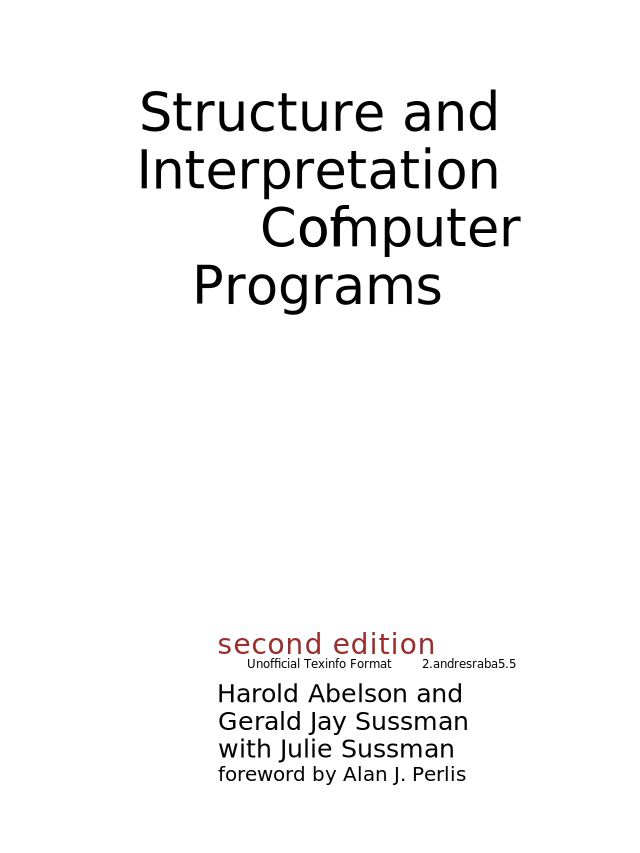
\includepdf[scale=0.92]{coverpage.pdf}

\pagebreak

\vspace*{\fill}
\thispagestyle{empty}

\begin{small}
%\begin{center}

\noindent
{\copyright}1996 by The Massachusetts Institute of Technology

\vspace{1.26em}
\noindent
Structure and Interpretation of Computer Programs,\\
second edition

\vspace{1.26em}
\noindent
Harold Abelson and Gerald Jay Sussman\\
with Julie Sussman, foreword by Alan J. Perlis

\vspace{1.6em}
\noindent

\includegraphics[width=25mm]{fig/icons/by-nc-sa.pdf}

\vspace{0.4em}
\noindent
This work is licensed under a Creative Commons\\
Attribution-NonCommercial-ShareAlike 3.0 Unported License\\
(\href{http://creativecommons.org/licenses/by-nc-sa/3.0/}{\acronym{CC BY-NC-SA} 3.0}).
Based on a work at \href{http://mitpress.mit.edu/sicp/}{mitpress.mit.edu}.

\vspace{1.26em}
\noindent
The \acronym{MIT} Press\\
Cambridge, Massachusetts\\
London, England

\vspace{1.26em}
\noindent
McGraw-Hill Book Company\\
New York, St. Louis, San Francisco,\\
Montreal, Toronto

\vspace{1.26em}
\noindent
Unofficial Texinfo Format \href{http://sicpebook.wordpress.com}{2.andresraba5.5} (September 15, 2015),\\
based on \href{http://www.neilvandyke.org/sicp-texi/}{2.neilvandyke4} (January 10, 2007).

\vspace{1.26em}
\noindent
日本語: by \href{http://github.com/minghai/sicp-pdf/}{minghai} based on 2.andresraba5.2 (March 31, 2014).
Decent Japanese version by \href{http://github.com/hiroshi-manabe/sicp-pdf/}{Hiroshi Manabe} based on 2.andresraba5.2 (October 12, 2015).

%\end{center}
\end{small}

\pagebreak

\tableofcontents

\small  % Added by minghai. (Japanese fonts looks too big.)

%=======================================================================================================

\chapter*{非公式Texinfoフォーマット}
\addcontentsline{toc}{chapter}{非公式Texinfoフォーマット}
\label{UTF}

これは\acronym{SICP}の非公式Texinfo版\yakuchu{
英語版にはTexinfo版がありますが、日本語版にはありません。{\LaTeX}ソースとPDFのみです。
}の第二版です。

あなたはきっと、これをEmacsのInfoモードのようなInfoハイパーテキストブラウザで読んで
いるのでしょう。もしかすると、{\TeX}で組版されたものを画面上で、または印刷して読んで
いるのかもしれませんね。もっとも、それは間抜けなことだと思いますが。それに、印刷するには
だいぶお金がかかりますよね。


\acronym{HTML}-\acronym{GIF}版は公式に無料で公開されているのですが、それを初めて
Unofficial Texinfo Format(非公式Texinfo版、\acronym{UTF})の初版としてLytha Aythが
個人的に変換したのは、2001年4月の長いEmacs Lovefest Weekendの間のことでした。



\acronym{UTF}は\acronym{HTML}版よりも検索が簡単です。また、あまりよくないコンピュータ
(たとえば寄付された386マシンのようなもの)を使っている人にとってもアクセスしやすいでしょう。
386マシンは、理論的には、Linux、Emacs、Schemeインタプリタを同時に実行できます。
しかし、多くの386マシンでは、Netscapeとそれに必要なX Window Systemの両方を動かそうとすると、
まだ始めたてでお金もない若いハッカーに\jnewterm{スラッシング}(\newterm{thrashing})という
概念を早い段階から教えるはめになるのがオチです。それに、\acronym{UTF}版なら圧縮なしで1.44\acronym{MB}
のフロッピーディスクに収まりますので、インターネットや\acronym{LAN}への接続環境のないPCに
インストールするのにも便利です。



Texinfoへの変換は、可能な範囲で直接的な翻字をしました。{\TeX}から\acronym{HTML}への
変換のように、これによってある程度内容が損なわれてしまいました。非公式TexInfo形式では、
図はいにしえの技術であるアスキーアートによって不格好に復活させられることになりました。
また、多量の上付き文字(`\^{}')と下付き文字(`\_')を変換するうちに、曖昧さによる変換ミスが
含まれてしまった可能性も大いにあります。どれが変換ミスかを当てるのは、読者への課題とします。
しかし、少なくとも私たちは、\emph{``より大きい''}という記号を\texttt{<u>\&gt;</u>}と符号化して
私たちの勇敢な宇宙飛行士たちを危険にさらすようなことはしていません。



もしあなたが\texttt{sicp.texi}を変更して間違いを直したりアスキーアートを改善したりした場合、
\code{@set utfversion 2.andresraba5.5}の行を更新し、あなたの差分を反映してください。
例えば、もしあなたがLythaのバージョン\code{1}から始めていて、あなたの名前がBobなら、改訂版には
\code{1.bob1}, \code{1.bob2}, \dots , \code{1.bob\textit{n}}のように名前をつけるのがいいでしょう。
また、\code{utfversiondate}も更新してください。もしあなたが自分の改訂版をWeb上で配布したいのなら、
文字列``sicp.texi''をファイルやWebページのどこかに埋め込んでおけば、Web検索エンジンから見つけ
やすくなるでしょう。




非公式Texinfo形式は、寛大にもフリーに配布されている\acronym{HTML}版の魂を引き継いで
いると信じられています。しかし、いつどこかの法律家の大艦隊が、何でもないような小さなことをめぐって
大騒ぎをしないとも限りません。ですから、あなたのフルネームを使ったり、あなたのアカウント名やマシン名を
含むかもしれないInfo, \acronym{DVI}, PostScript, \acronym{PDF}版を配布したりするのは
慎重に考えてからにしてください。

\noindent
\textit{Peath, Lytha Ayth}

\vspace{1.0em}
\noindent
\textbf{付録:}AbelsonとSussmanによる\acronym{SICP}のビデオレクチャーもご覧下さい。\\
\href{http://groups.csail.mit.edu/mac/classes/6.001/abelson-sussman-lectures/}{\acronym{MIT CSAIL}}, 
\href{http://ocw.mit.edu/courses/electrical-engineering-and-computer-science/6-001-structure-and-interpretation-of-computer-programs-spring-2005/video-lectures/}{\acronym{MIT OCW}}.

\vspace{0.5em}
\noindent 
\textbf{付録2:} 上記は2001年の元の\acronym{UTF}の紹介です。
10年後のいま、\acronym{UTF}は一変しました。数学上の記号と式は適切に組版され、図は
ベクターグラフィックにより描かれています。元のテキスト形式とアスキーアートの図
は今でもTexinfoのソースに残っていますが、表示されるのはInfo形式にコンパイルした場合だけです。
電子書籍リーダーとタブレットの夜明け時代になって、画面上で\acronym{PDF}を読むことは、もはや
バカバカしいことではないとはっきり言えるようになりました。
楽しんでください!

\vspace{0.5em}
\noindent
\textit{A.R, May, 2011}

%============================================================================================================
\chapter*{非公式日本語版}
\addcontentsline{toc}{chapter}{非公式日本語版}
\label{Unofficial Japanese Edition}

SICPはかつて第一版、第二版共に日本にて公式に翻訳が商業出版されていました。
第二版を出版していたピアソン桐原が2013年8月に
\href{http://slashdot.jp/story/13/08/09/0517250/}{ピアソングループから撤退し技術書の取扱を終了したため}、
日本語でSICPを読む機会は失われました。
このことがこの翻訳を行うことの契機となりました。

実際にはその後、2014年1月付近に、寛大にも第二版の訳者、和田英一先生がオンライン上にてSICPの訳書、
\href{http://sicp.iijlab.net/}{「計算機プログラムの構造と解釈」}全文を公開して下さいました。この時点でこの非公式日本語版の
価値は随分と小さくなりました。

しかし、その時、既に3章まで翻訳していたこと、そして非公式TexInfo版が2013年11月に大改訂を行い、
当初の日本語には正式に対応していないtexi2pdfから変更を行い、XeLaTeXを採用したために、
日本語でも美しい組版ができる可能性が出てきたことが、この原稿を廃棄することを押し止めました。

SICPのライセンスについてはインターネットアーカイブにて調べてみました。
2001年1月にMITがSICPを寛大にもオンラインで無料で読むことができるように公開された時にはライセンスが指定されていませんでした。

2008年4月にMITはSICPのライセンスをCC BY-NCと指定しました。その後ライセンスは2011年10月に一旦CC BY-SAに変更されます。
そして2年後の2013年9月に再びCC BY-NCへと戻されました。この事実がSICP原文のライセンスの解釈を難しくしています。
ライセンスの変更はオーナーの自由ですが、ライセンシーはコンテンツ取得時のライセンスを尊重すれば良いからです。

最初に非公式TexInfo版を作成したLytha Aythはライセンス指定の無いSICP公開をWeb文化に基づくものだと理解しました。
次にLaTeXの組版を開発したAndres RabaはCC BY-SAに基き正式な許諾の下、PDF版を作成しました。
私の翻訳はPDF版のライセンスであるCC BY-SAに従うことが求められます。しかし、現在のMITが非商業を求めて
いることを鑑みて、Raba氏に許可を頂いた上で非商業制約を追加した
\href{http://creativecommons.org/licenses/by-nc-sa/3.0/}{\acronym{CC BY-NC-SA} 3.0}
にてリリースすることにしました。

CC BY-NC、及びBY-SAは共に翻訳の許可を明記しています。従ってこの翻訳にはLythaが心配したような法的問題は
起こらないと信じています。しかし同時に、法的問題は常に一方的に起こされることがあることもまた現実です。
従って読者の皆様には常にネットワーク上のデータは(そしてプログラムも!)消えてなくなってしまうシャボン玉で
あることを忘れずに御用心願います。

TeX、LaTeX環境の日本語対応を進めて下さった全ての関係者の皆様に感謝します。
特に最新の情報を常に更新し続けて下さっている\href{http://oku.edu.mie-u.ac.jp/~okumura/texwiki/}{TeX Wiki}の奥村~晴彦氏、
W32TeXを自動でインストールし更新可能な
\href{http://www.math.sci.hokudai.ac.jp/~abenori/soft/abtexinst.html}{TeXインストーラ}作者の阿部~紀行氏、
XeLaTeX向け日本語パッケージ
\href{http://zrbabbler.sp.land.to/zxjatype.html}{``ZXjatype''}
を開発して下さった八登~崇之氏に感謝致します。

海外ではSICPの新しい形の開発が非常に盛んです。PDFはもちろん、epubやインタラクティブ版、Kindle版(mobi形式)、ClojureやJavaScriptに
よるSICP等が公開されています。この翻訳はCC BY-NC-SAですので非商業であればそのような
派生や翻案に利用することが可能です。日本でもSICPの世界が広がっていくことを期待しています。

\vspace{1em}
\noindent
※ 校正御協力者様 (順不同、敬称略)

\begin{itemize}

\item \href{https://github.com/kei-s}{Kei Shiratsuchi}

\item \href{https://github.com/kimurakoichi}{Kimura, Koichi}

\item \href{https://github.com/nna774}{のな}

\item \href{https://github.com/ainoya}{Naoki Ainoya}

\end{itemize}

%============================================================================================================
\chapter*{非公式日本語版 翻訳改訂版}
\addcontentsline{toc}{chapter}{非公式日本語版 翻訳改訂版}
\label{Unofficial Japanese Edition Revised Translation}

この翻訳改訂版は、minghai氏の非公式日本語版(以降、minghai氏版)の翻訳に不十分なところが多かったため、
原著から翻訳をし直したものです。この翻訳を進めるにあたっては、minghai氏版の訳を置き換えていくと
いうやり方で進めていきました。しかし、差分を取ればわかっていただけると思いますが、minghai氏版の
テキストは痕跡をとどめていないはずです。この方式を採ったのは、主にモチベーション上の理由によるものです。
もしminghai氏版の痕跡が(誰が訳しても同じようになるものを除いて)あるとすれば、それは作業漏れが
残っているということですので、ご報告いただければ幸いです。

用語については、無用の混乱を避けるため、和田英一氏によるオンライン版\href{http://sicp.iijlab.net/}
{「計算機プログラムの構造と解釈」}(以下、和田氏版)にできるだけ追従するようにしました。
もちろん、訳文はすべて自分で一から作り上げたものです。用語の追従によって著作権やライセンス上の
問題が発生することはないと信じていますが、問題があるようであればお教えいただければと思います。

私としては、もしminghai氏版がなければ、和田氏版の訳書を購入して勉強して、それで済ませていたはずの
ところです。訳文は硬いとはいえ読めないことはなく、英語で読むよりは速く進められそうでした。
ほかのこなれていない訳書同様、不満を持ちながら読み、それで終わりだったはずです。

しかし、minghai氏版が出てきたことで、状況は大きく変わりました。minghai氏版は無料のPDFなので、
有料の書籍とオンラインHTMLという和田氏版よりアクセスが容易です。さらに、和田氏版は(Amazonの
レビューにもあるように)翻訳の評判がよくありませんが、minghai氏版はですます調で一見親しみやすく、
翻訳に問題が多いということがすぐにはわかりません。

これでは、SICPの評判を聞いて勉強しようとした人が、minghai氏版に流れてしまうのではないか。
私のその危惧は、Twitterのタイムラインで現実化していました。タイムラインでもminghai氏版に手を
伸ばそうとしている人がいたため、和田氏版をお勧めしておきました。もちろん、その人は氷山の一角で、
実際には少なからぬ人たちがminghai氏版に流れたのではないかと思います。

文体が硬くて意味の取りにくい翻訳の場合、読者はなんとか読み解く努力をするか、読むことをあきらめて
訳者を責めるか(これはAmazonレビューで起こっていることです)のどちらかの行動を取るでしょう。
後者の人に対しては(有料で購入した場合)金銭的な損害を与えているかもしれませんが、それがすべてです。
どうしても読みにくければ、原文で読むことになるでしょう。いずれにせよ、翻訳が存在しなかった場合以上に
悪いことにはなりません。

しかし、表面上読みやすそうな問題の多い翻訳は、はるかに大きな副作用をもたらす可能性があります。
実際には誤訳のために訳文が意味不明になっているだけなのに、理解できないのは書いてある内容が
難しすぎるためだ、それを理解するだけの頭脳が自分にないためだ、と読者は思い込んでしまうかも
しれません。それだけはどうしても避けたいところです。

それらのことを考え合わせた結果、SICP を原文から翻訳しながら勉強していくことにしました。
始めたとき、毎日一時間というペースで進めていくと決め、数日間やってみた進捗状況から翻訳が
終わるまでの期間を見積もったところ、どうやら一年ぐらいかかりそうだとわかりました。一年と
いうのは長い時間です。心がくじけそうになりつつも、ミヒャエル・エンデの「モモ」を思い出し、
その日その日の分だけを考え、続けていきました。毎日夜9時からを定刻としていたため、Twitterでは
「時報」と言ってくれる人もいました。

そして先日、ようやく翻訳とチェック作業が終わりました。期間は予定通り一年程度でした。勉強を
兼ねての翻訳だったため、中身を理解しながら、練習問題もできるだけ(といっても、\link{第3章}の
途中あたりでリタイアしましたが)解いていきました。前評判に違わず、SICPの内容はとても充実して
いました。翻訳前に危惧していたような、「この時間で何ができたか」と後悔するようなことには
ならずにすみました。

もちろん、私のこの翻訳が完全だとは思っていません。しかし、致命的な誤訳が何百箇所もあって
どこから手をつけていいかもわからないような訳文でないことは保証します。
この本の内容が理解できないとすれば、それは翻訳がおかしいからではありません。もちろん、
内容が難しすぎるためでも、それを理解するだけの頭脳がないためでもありません。足りないのは
時間をかけた読み込みです。じっくりと一文一文の意味を考え、サンプルコードを動かし、できるだけ
練習問題を解いていけば、それで十分です。この本は、読者を置き去りにしようとするような本では
ありません。

最後に、日本語版のテンプレートを提供していただいたことについて、minghai氏に深く感謝します。
minghai氏の日本語版テンプレートがなければ、私の{\TeX}や{\LaTeX}についての限られた知識では
日本語訳を行うことはできなかったでしょう。

それでは、SICP日本語版をお楽しみください。

真鍋宏史

%============================================================================================================


\chapter*{献辞}
\addcontentsline{toc}{chapter}{献辞}
\label{Dedication}



この本を、尊敬と賛美を込めて、コンピュータの中に住む妖精に捧げます。

\begin{quote}
``コンピュータサイエンスに関わる私たちにとって、コンピューティングを
楽しむことはとても大事だと私は思っています。コンピューティングの始まりの時期には、
それはとても楽しいことでした。
ご存じのとおり、お金を払うお客様たちが騙されるということがそこかしこで起こり、
それからしばらくして、私たちは彼らの不満を真面目に受け取るようになりました。
私たちは、あたかもコンピュータをきちんとエラーなしで完璧に使えるようにすることが
私たちの責任であるかのように考え始めてしまいました。
私はそうは思いません。
私たちは、コンピュータを発展させ、新しい方向に向かわせ、家の中で楽しめるように
しておくことに責任があると思います。コンピュータサイエンスのその分野が、
ずっとその楽しさの感覚を失わないでくれればと願っています。特に、私たちが伝道師に
なったりしないことを望んでいます。聖書のセールスマンのような感覚を持たないでください。
そんな人たちは、もう世界に十分すぎるほどいます。あなたがコンピューティングについて
知っていることは、ほかの人たちも学ぶことができます。
コンピューティングをうまくやる鍵が、あなたの手の中にしかないとは思わないでください。
あなたの手の中にあるものは知性だと、私は思い、またそうであることを願っています。
それはつまり、あなたが出会ったマシンに対して、出会ったときよりも多くのものを見ることが
できる能力です。そして、それをそれ以上のものにできる能力です。''

\noindent
---Alan J. Perlis (April 1, 1922 -- February 7, 1990)
\end{quote}

%===========================================================================================================


\chapter*{前書き}
\addcontentsline{toc}{chapter}{前書き}
\label{Foreword}

\vspace{-0.6em}


教育者、将軍、栄養士、精神分析医、そして両親は、計画を立て(program)ます。
軍隊や学生は計画によって動いていますし、計画によって動いている社会もあります。
大きな課題に取り組むときにはいくつもの計画を使いますが、それらのほとんどは
問題に取り組む中で生まれるものです。
それらの計画には、そのとき取り組んでいる課題に特化しているように見える問題があふれています。
計画を立てるということ自体を知的な活動として理解するためには、コンピュータ
プログラミングに目を向ける必要があります。コンピュータプログラムを読み書きする必要があります---
それも、大量に。何のプログラムか、どういう応用のためかというところはあまり重要ではありません。
重要なのは、それらがどのようにふるまい、またより大きなプログラムを作る中でそれらがどれだけスムーズに
ほかのプログラムと協調できるかということです。プログラマは、部品の完全性と、
組み合わせたものの妥当性の、両方を追求しなければいけません。この本では、``プログラム''
というのは、Lispのある方言で書かれた、デジタルコンピュータ上で実行されることを前提とした
プログラムの作成・実行・研究に焦点を当てています。Lispを使うことは、プログラムの記述について制約を
加えるだけで、何をプログラムするかを制約するものではありません。

この本の主題について考えるうえで、3つの事象を考えることになります。
人間の心、コンピュータプログラムの集合、そしてコンピュータです。
コンピュータプログラムはすべて、実際のプロセスや精神的なプロセスのモデルであり、
人間の心の中で生まれるものです。
これらのプロセスは、人間の経験と思考から浮かび上がってくるもので、数はとても多く、
細かいところまで入り組んでいて、いつでも部分的に理解することしかできません。
それらがコンピュータプログラムとして永遠に満足できるようにモデル化されるなんて
いうことは、めったにありません。ですから、私たちのプログラムは、注意深く工夫された
バラバラの記号の集合であり、絡まり合う関数の組み合わせでありながらも、絶えず
進化していきます。私たちのモデルに対する理解が深まったり、広がったり、一般化したり
するたびに、私たちはプログラムに手を加えていきます。最終的に、モデルは準安定状態に
達し、それは私たちが取り組む別のモデルの中に位置を占めることになります。
コンピュータプログラミングに関する興奮の源は、プログラムとして表現されたメカニズムが
私たちの心の中とコンピュータ上で絶え間なく広がっていくことと、またそれが生み出す
知覚の爆発です。芸術が私たちの夢を解釈するものだとすると、コンピュータは夢を、
プログラムという形で実行するものなのです!

コンピュータは強力ですが、厳しい親方でもあります。プログラムは正しくなければ
ならず、伝えたいことは細かいところまで正確に伝えなければいけません。
ほかのすべての記号的な活動と同じく、プログラムが真であることは論証によって
知ることができます。Lispはそれ自身、意味論(これもまたモデルです)を割り当てることが
でき、そしてプログラムの仕様が、例えば述語論理などによって決められるのであれば、
論理学の証明方法によって、容認可能な正確性の論証をすることができます。
残念ながら、プログラムが大きく複雑になるにつれ(いつもそうなるのですが)、
仕様自体の妥当性、一貫性、正しさが疑わしいものになっていきます。そのため、
完全な形式的な正しさの論証というものが大きなプログラムについてくるということは
めったにありません。大きなプログラムは小さなものから成長していくものなので、
正しさについて確信を持てるような標準的なプログラム構造(これをイディオムと呼びます)
の武器庫を作り上げ、確立された組織化技術によってより大きな構造に組み立てていく方法を
学ぶことが決定的に重要になります。この本では、それらの技術について詳細に扱っていきます。
それらを理解することは、プロメテウスのような創造的な営みであるプログラミングという
分野に加わるためには不可欠なことです。何よりも、
強力な組織化の技術を発見し身につけていくことによって、大規模で重要なプログラムを書くに
あたって必要となる能力を育てることができます。また逆に、大規模なプログラムを書くことは
負担がとても大きいということもあり、何とか新しい手法を発明して、大規模なプログラムに
組み込む関数や実装の量を減らすことができないかと考えていくことになります。

プログラムとは違って、コンピュータは物理法則に従わなければなりません。もし
素早く---状態遷移あたり数ナノ秒といったレベルで---動作したければ、電子をほんの
短い距離(せいぜい\(1{1\over2}\) フィートだけ)しか運ぶことができません。
空間的にぎっしり詰め込まれた膨大な数のデバイスが発する熱は、取り除く必要があります。
高機能性とデバイス密度のバランスを取りながら、精緻な工学的技法が
発展してきました。いずれにせよ、ハードウェアは私たちがプログラムしようとしている
レベルよりも基礎的なレベルで動いています。私たちのLispのプログラムを
``機械の''プログラムに変換する処理は、それ自身が抽象的なモデルで、それは
私たちがプログラムするものです。その研究と作成は、どんなモデルをプログラムするとき
にも関わってくるような組織的プログラムについて、多くの洞察を与えてくれます。
もちろん、コンピュータそれ自身もそのようにモデル化されています。考えてみてください。
一番小さい物理的なスイッチング素子は量子力学によってモデル化され、量子力学は
微分方程式によって記述され、微分方程式の詳細なふるまいは数値近似によって表され、
数値近似はコンピュータプログラムによって表現され、そのコンピュータプログラムは
コンピュータによって実行され、そのコンピュータを構成する素子は\( \dots \)!

3つの焦点を別々に設定することは、単なる方法上の便利さのためだけではありません。
よく「すべては頭の中のことだ」と言われますが、このように論理的に分けることによって、
これらの焦点の間の記号的通信を促進できます。人間の経験の中で、これら3つの
豊かさ、生命力、潜在力を超えるものは、人生そのものの発展ぐらいです。これらの焦点の
間の関係は、せいぜい準安定状態です。コンピュータの容量の大きさや速さは、これで十分と
なることは決してありません。ハードウェア技術の進歩のたびに、より大きなプログラミング
の取り組み、新しい組織化原則、そして抽象モデルの発展が引き起こされます。読者は、
定期的に``どこに向かっているんだ? どこに向かっているんだ?''と自問しなければなりません。
---でも、あまり問いすぎないようにしましょう。そうでないと、ほろ苦い哲学的な便秘のために、
プログラミングの楽しさを見逃してしまうことになります。

私たちが書くプログラムの中で、一部のもの(しかし、決して十分にはならない)は、
並べ替え、数列の最大値を見つける、素数性判定、平方根の計算といった、精密な
数学的な関数を実行します。そのようなプログラムはアルゴリズムと呼ばれ、その最適な
ふるまいについては多くのこと(特に、実行時間とデータストレージの必要量という
二つのパラメータについて)が知られています。プログラマは、よいアルゴリズムと
イディオムを身につけなければなりません。プログラムの中には厳密な仕様が記述しにくい
ものもありますが、プログラマとしては責任を持ってパフォーマンスを推定し、また
常に改善しようとしなければなりません。

Lispは、``生き残ったもの''です。約四半世紀にわたって使われてきています。
活発なプログラミング言語の中で、これより長い時間を生きてきたものはFortranだけです。
どちらの言語も、重要な応用領域でのプログラミングの必要性を支えてきています。
Fortranは科学計算と工学計算を支え、Lispは人工知能を支えてきました。この二つの分野は
今でも重要であり続け、これらの分野のプログラマはLispとFortranという二つの言語に
力を注いでいるので、少なくとももうあと四半世紀の間活発に使われる言語であり続ける
ということは十分ありうることです。

Lispは変化します。このテキストで使っているScheme方言は、オリジナルのLispから進化
してきたもので、いくつかの重要な点で異なっています。例えば、変数束縛のための
静的スコーピングや、関数が関数を値として返すことを許可することなどです。構文的な
構造において、SchemeはAlgol 60に似ています。その近さは、Schemeと初期のLispとの
近さと同じ程度です。Algol 60は、もう活発な言語になることはないでしょうが、Schemeと
Pascalの遺伝子の中に生き続けています。これら二つの言語ほど、かけ離れた文化に
取り囲まれ、その流通貨幣となっているような二つの言語というのもなかなかないでしょう。
Pascalはピラミッドを建てるためのものです。雄大で、息をのむような、静的な構造物で、
軍隊が重い石を運び、所定の位置に押しこむことによって作られています。
Lispは有機体を作るためのものです。雄大で、息をのむような、動的な構造物で、小さな
チームが無数のより単純な揺れ動く有機物を所定の位置に入れることによって作られています。
どちらの場合にも、組織化のための原則は同じですが、ひとつだけ非常に重要な違いがあります。
個々のLispプログラマに委ねられたエクスポート可能な関数は、Pascal企業の中で見つけられる
ものより桁違いに多いのです。Lispのプログラムは、本来目的としていたアプリケーションを
超えた有用性を持つ関数でライブラリをいっぱいにします。そのように有用性が増加していく
背景には、リストというLispのネイティブデータ構造の存在があります。リストの単純な
構造と自然な適用可能性は、驚くほど普遍的な関数という形で表れてきます。Pascalでは、
宣言可能なデータ構造の多さが関数の専門化を引き起こし、気軽な連携は禁じられ、
ペナルティを与えられるものとなります。ひとつのデータ構造を扱う100の関数があるほうが、
10のデータ構造を扱う10の関数があるのよりもよいのです。結果として、ピラミッドは
千年もの間変化せずに存在しつづけなければならないのに対し、有機体は存在する限り
進化し続けなければなりません。進化を止めるということは滅びることを意味します。

この違いをはっきり知るためには、この本の中での教材と練習問題の扱いを、何でもいいので
Pascalを使った入門テキストと比べてみてください。このテキストは\acronym{MIT}でしか
消化できない、\acronym{MIT}に固有の種族のためのものだとかいった妄想は抱かないでください。
このテキストは、真面目なLispのプログラミングの本はどのようなものでなければいけないか
というところを形にしたものであり、学生が誰であるか、どこで使われるかは関係ありません。


ひとつ気をつけておいていただきたいのは、この本はプログラミングに関するテキストだと
いうことです。ほとんどのLispの本は人工知能に使うための準備となっていますが、この本は
違います。いずれにしても、対象となるシステムが大きくなるにつれ、ソフトウェア工学と
人工知能に関わる重要なプログラミング上の課題は融合していく傾向にあります。まさに
そのために、人工知能以外の領域でも、Lispに対してこれほどの関心が向けられているのです。


その目的とするところから予想できる通り、人工知能の研究は数多くの重要なプログラミングの
問題を生み出しています。ほかのプログラミング分野であれば、このような大量の問題に対しては
新しい言語が生み出されるところです。実際に、非常に大きなプログラミングのタスクにおいて、
組織化のために便利な方法のひとつは、新しい言語を発明して、タスクモジュールの中に通信を
閉じ込め、コントロールするということです。これらの言語は、私たち人間が頻繁にやりとりを行う
システムの周辺部に近づくにつれて、単純でなくなっていく傾向があります。その結果、
そのようなシステムでは、複雑な言語処理の機能が何回も繰り返し実装されることになります。
Lispは、非常に単純なシンタックスとセマンティクスを持つため、パージングは初歩的なタスクとして
扱うことができます。ですので、パージング技術はLispのプログラムの中でほとんど何の役割も
果たしません。また、大きなLispのシステムが成長し変化していく中で、言語処理系の構築が
その成長速度の妨げになることはめったにありません。最後になりますが、このシンタックスと
セマンティクスの単純さこそが、すべてのLispプログラマが付き合うことになる重荷と自由の
源泉になっているのです。数行以上のLispプログラムを書こうとすると、必ず自由に使える関数で
いっぱいになります。発明し、組み込み(fit)ましょう。かんしゃくを起こし(have fits)、
再発明しましょう! 括弧のネストの中に自分の考えを書いていくLispプログラマに乾杯。


\vspace{0.5em}
\noindent
Alan J. Perlis\\
New Haven, Connecticut

%=========================================================================================================


\chapter*{第二版~序文}
\addcontentsline{toc}{chapter}{第二版~序文}
\label{Preface}

\begin{quote}
ソフトウェアが、ほかの何にも似ていないということはあるでしょうか。それは捨てられる
ためのもので、常にシャボン玉のように見ることがすべてだと。

---Alan J. Perlis
\end{quote}

\vspace{0.7em}

\noindent
この本で扱われている題材は、1980年から\acronym{MIT}の入門レベルの計算機科学科目の基礎と
なってきました。初版が発売されたとき、すでにこの教材を使った授業を4年間行っていました。
この第二版が出てくるまでには、それからさらに12年が過ぎています。私たちの成果が広く受け入れられ、
ほかのテキストにも取り込まれていることについて、私たちはうれしく思っています。私たちは、学生たちが
この本に出てくる考え方やプログラムを身につけ、それらを新しいコンピュータシステムやコンピュータ言語の
核として組み込むのを見てきました。古代のタルムードに出てくる言葉遊びを文字通り実現し、私たちの学生は
建築者になったのです。このような有能な学生、功績ある建築者を得ることができたのは幸運なことでした。

この版の準備にあたって、何百にものぼるわかりやすい説明を取り込みました。それらは、私たち自身の
教育経験や、\acronym{MIT}やほかの場所の同僚たちのコメントから得られたものです。この本に出てくる
主なプログラミングシステムのほとんどを再設計しました。それには一般計算システム、インタプリタ、
レジスタマシンシミュレータ、コンパイラが含まれます。さらに、プログラムの例をすべて書き換え、
\acronym{IEEE} Scheme標準(\link{IEEE 1990})に適合したScheme実装であればどんなものの上でも
コードを実行できるようにしました。

この版では、いくつかの新しいテーマに重点を置いています。これらの中で最も重要なものは、
計算モデルの中で時間を扱うさまざまなアプローチの中心的な役割を果たしているものです。
それらのアプローチには、状態つきのオブジェクト、並行プログラミング、関数型プログラミング、
遅延評価、非決定性プログラミングがあります。並行性と非決定性については新たに節を設け、
本全体を通してこのテーマを統合させるよう力を尽くしました。

この本の初版は、\acronym{MIT}の半期の科目のシラバスをなぞったものでした。第二版では、
多くの新しい題材を含めたため、半期ですべてをカバーするのは無理でしょう。ですので、
講師は教えるべき内容を選ぶ必要があります。私たち自身が講義をする際には、時々
論理プログラミング(\link{4.4節})を飛ばします。学生にはレジスタマシンのシミュレータを
使わせますが、その実装(\link{5.2節})はやりません。そして、コンパイラ(\link{5.5節})
はざっと概要を見るだけです。それでもなお、これは中身の濃い授業です。講師によっては、
最初の3章か4章だけをやって、残りの題材は次の科目に譲りたいという人もいるでしょう。

World-Wide-Webサイト \href{http://mitpress.mit.edu/sicp}{http://mitpress.mit.edu/sicp} は、
この本の読者に対するサポートを提供しています。それには、この本に出てくるプログラム、プログラミング
練習問題のサンプル、補助教材、ダウンロード可能なLispのScheme方言の実装が含まれます。

%============================================================================================================

\chapter*{第一版~序文}
\addcontentsline{toc}{chapter}{第一版~序文}
\label{Preface 1e}

% \vspace{-0.6em}
\begin{quote}
コンピュータはバイオリンのようなものです。次のような場面を想像してみてください。
ある初心者の人が、まず蓄音機を動かしてみて、それから次にバイオリンを触ってみます。
その人は、バイオリンの音はひどいと言います。人間主義者たちや多くの計算機科学者から
私たちが聞く話はそういったものです。コンピュータのプログラムは特定の目的にはよいが、
柔軟ではないと。バイオリンやタイプライターだってそんなものです。使い方を学ばなければの
話ですが。

---Marvin Minsky, ``Why Programming Is a Good Medium for Expressing
Poorly-Understood and Sloppily-Formulated Ideas''
\end{quote}

\vspace{0.8em}

\noindent
``The Structure and Interpretation of Computer Programs''(SICP, 計算機プログラムの構造と解釈)は
マサチューセッツ工科大学(MIT)での入門者レベルの計算機科学の科目です。\acronym{MIT}
で電気工学や計算機工学を専攻する学生はすべて、4つある``共通コアカリキュラム''の
ひとつとして履修しなければなりません。残りは、回路と線形システムについての
科目2つと、デジタルシステム設計の科目ひとつです。私たちは、この科目の開発に1978年から
携わってきました。そして、1980年の秋からは、この教材の現在の形で毎年600人から700人の
学生を教えてきています。ほとんどの学生はコンピュータについてそれまでまったく秩序立った
トレーニングを受けていないか、受けていてもわずかなものでした。とはいえ、コンピュータで
ちょっと遊んだことのある学生は多くいましたし、プログラミングやハードウェア設計に相当な
経験のある学生も数人はいましたが。

私たちがこの計算機科学の入門科目の授業計画を策定するにあたって、二つの懸念点を
内容に反映させました。一つ目は、コンピュータ言語はただコンピュータに操作を
実行させる方法であるにとどまらず、方法論についての考え方を表現するための
今までにない形式的媒体であるという考え方を打ち立てたいということでした。
ですから、プログラムは人間が読めるように書かなくてはならず、それがたまたま
機械によって実行できるというだけのことです。二つ目は、私たちがこのレベルの科目で
扱われるべき中心的な題材について信じていることです。教えるべきはことは、
特定のプログラミング言語の文法ではなく、また特定の関数を計算するための賢い
アルゴリズムでもなく、さらに言うとアルゴリズムの数学的解析やコンピューティングの
基礎ですらなく、重要なのは大きなソフトウェアシステムの知的複雑性をコントロールする
技術であるということです。

私たちの目標は、この科目を修了した学生たちが、プログラミングのスタイルと美学について、
基礎的な感覚を十分に身につけてくれることです。学生たちが、大きなシステムの複雑性を
コントロールするための主要な技術を使いこなせるようになること。模範的なスタイルで
書かれていれば、50ページにわたるプログラムでも読めるようになっていること。どんなときにも、
何を読むべきでないか、何を理解しないでもいいかを判断できるようになること。
また、プログラムを変更するにあたって、自信を持って、元の作者の意図とスタイルを保ったままで
変更を加えることができるようになっていること。

これらのスキルは、決してコンピュータプログラミングに特有のものではありません。
私たちが教え、また利用する技術は、すべての工学的設計に共通するものです。私たちは、
詳細な部分を隠す抽象化を適宜加えることによって、複雑性をコントロールします。
私たちは、共通のインターフェイスを確立し、標準的かつ中身のよくわかっている部品を
「うまく組み合わせる」やり方で、複雑性をコントロールします。私たちは、設計を
記述するためにさまざまな言語を作り出し、それぞれの言語が設計のある特定の側面を際立たせ、
それ以外の側面を目立たなくさせることによって、複雑性をコントロールします。

私たちのこの科目に対するアプローチの底にあるものは、``計算機科学''は科学ではなく、
その意義はコンピュータとほとんど関係がないという信念です。コンピュータ革命とは、
私たちの考え方と、考えを表現するやり方の革命です。この変化を象徴する出来事は、
\jnewterm{手続き的認識論}(\newterm{procedural epistemology})---古典的な数学的テーマで
取られるような宣言的な見方ではなく、命令的な見方による知識構造の研究---の出現でしょう。
数学は、``何であるか''という考えについて正確に扱う枠組みを提供します。計算機科学は、
``どうやるか''という考えについて正確に扱う枠組みを提供します。

この教材では、プログラミング言語Lispのひとつの方言を使います。言語を正式に
教えることはしません。その必要がないからです。普通に使っていくだけで、数日のうちに
学生は身につけます。これはLisp系の言語の大きな利点です。複合式を作るやり方は
少ししかなく、構文構造はあってないようなものです。形式的な性質はすべて、
チェスのルールのように、一時間もあればカバーできます。少ししたら、言語の
構文的な詳細について忘れてしまい(元からそんなものはないので)、実際の問題---
何を計算したいのか、どうやって問題を扱えるサイズの部品に分解するか、
それらの部品をどのように作っていくか---に取り組むことになります。
もうひとつのLispの利点は、私たちの知る限りほかのどんな言語よりも、プログラムを
モジュールに分解する大規模な戦略をサポートしてくれる(しかし強制はしない)という
ところです。手続きやデータによる抽象化をしたり、よくある使い方のパターンを
捉えるために高階関数を使ったり、代入とデータ変更によって局所状態をモデル化したり、
ストリームと遅延評価によってプログラムの部品同士を連携させたりといったことが可能です。
さらに、組み込み言語の実装も簡単にできます。また、これらすべては、
漸進的なプログラム設計、構築、テスト、デバッグに対する優れたサポートを
提供する対話的環境に埋め込まれています。これまでにないパワーと優美さを備えた
すばらしいツールを作り上げたJohn McCarthyをはじめ、これまでのすべての世代の
Lispウィザードたちに感謝の気持ちを捧げます。

私たちが使うLispの方言であるSchemeは、LispとAlgolのパワーと優美さを
ひとつにまとめようとしたものです。Lispからは、シンプルな構文によるメタ言語的なパワー、
プログラムをデータオブジェクトとして表す統一的なやり方、ガベージコレクションつきヒープへの
データ割り当てが取り込まれています。Algolからは、レキシカルスコープとブロック構造を
取り込んでいます。これらは、Algol委員会のプログラミング言語設計の先駆者たちからの
贈り物です。チャーチの\( \lambda \)計算とプログラミング言語の構造との間の関係についての
洞察はJohn ReynoldsとPeter Landinによるものです。また、コンピュータが世界に現れる
何十年も前からこの領域を探索してきた数学者たちに対する恩義も感じています。
彼ら開拓者たちには、Alonzo Church, Barkley Rosser, Stephen Kleene, Haskell Curryなどが
含まれます。


%============================================================================================================

\chapter*{謝辞}
\addcontentsline{toc}{chapter}{謝辞}
\label{Acknowledgements}


この本とこのカリキュラムの開発を手助けしてくださった多くの方々に感謝いたします。


私たちの科目は、明らかに``6.231''の知的な系譜を継ぐものです。それは、1960年代後半に
\acronym{MIT}でJack WozencraftとArthur Evans, Jr.が担当していた、プログラミング言語学と
\( \lambda \)計算についてのすばらしい科目でした。


Robert Fanoが\acronym{MIT}の電気工学と計算機科学の入門カリキュラムを再編成し、
工学設計の原理に重点を置くようにしてくれたことに非常に感謝しています。
彼はこの取り組みを始めるよう私たちを導き、最初の科目ノートをまとめてくれました。
この本は、それをもとに発展してきたものです。


私たちが教えようとしているプログラミングのスタイルと美学は、その多くが
Guy Lewis Steele Jr.と連携して開発したものです。彼は、Gerald Jay Sussmanとともに
Scheme言語の初期の開発に携わりました。さらに、David Turner, Peter Henderson,
Dan Friedman, David Wise, Will Clingerは、この本に登場する関数プログラミング
コミュニティのテクニックを数多く教えてくれました。


Joel Mosesは、大きなシステムを構築する方法を教えてくれました。彼は、記号計算に使われる
Macsymaシステムでの開発経験を通して、制御の複雑性を回避して、モデル化しようとしている
世界の現実の構造を反映するようデータを体系化することに集中することが重要だということを
学んでいました。


Marvin MinskyとSeymour Papertは、プログラミングと、知的生活の中でそれをどのように
位置づけるかについて、私たちの姿勢の多くを形作ってくれました。コンピュータがなければ
正確に扱うには複雑すぎるような考えを探究するにあたって、コンピュータが表現手段を
与えてくれるということを理解できるようになったのは彼らのおかげです。彼らは、
学生のプログラムを書き、変更する能力が、自然活動を探究するための強力な方法になると
強調しています。


私たちはまた、プログラミングはとても楽しいものであり、プログラミングの楽しみを支える
よう注意しなければいけないというAlan Perlisの考え方に強く同意します。この楽しみの
一部分は、偉大な職人たちの働いているところからも得ることができます。
Bill GosperやRichard Greenblattのもとで見習いプログラマとして働けたことは
幸運なことでした。


私たちのカリキュラムの開発に貢献してくださったすべての方々について名前を挙げるのは
困難です。過去15年間私たちと共に働き、私たちの科目に多くの時間を費していただいた
すべての講師、口頭の指導者、チューターたち、中でもBill Siebert,
Albert Meyer, Joe Stoy, Randy Davis, Louis Braida, Eric Grimson, Rod Brooks, Lynn Stein,
Peter Szolovitsに感謝します。現在はウェルズリーにいるFranklyn Turbakに、教育上の
際立った貢献について特に感謝します。彼の学部生向けの授業は、私たち皆が目指す基準を
打ち立てました。Jerry SaltzerとJim Millerには、私たちが並行性のミステリーに取り組むのを
手助けしてくださったことを感謝します。そしてPeter SzolovitsとDavid McAllesterには、
\link{第4章}における非決定性評価の説明に対する貢献に感謝します。


多くの方々が、他大学でこの資料を紹介するのに大きな努力を費してくださいました。
中でも私たちが緊密に連携していたのは、イスラエル工科大学のJacob Katzenelson、
カリフォルニア大学アーバイン校のHardy Mayer、オックスフォード大学のJoe Stoy、
パデュー大学のElisha Sacks、ノルウェー技術科学大学のJan Komorowskiです。
私たちは、他大学にこの科目を適合させることで主要な教育の賞を受けた同僚たちを
非常に誇りに思います。この中には、イェール大学のKenneth Yip、カリフォルニア大学
バークリー校のBrian Harvey、コーネル大学のDan Huttenlocherが含まれます。


Al Moy\'eは、ヒューレット・パッカードの技術者にこの教材を教え、その講義を
ビデオテープにすることを手配してくれました。これらのビデオを使った生涯教育の
コースを計画し、世界中の大学や企業で教えた有能な講師たち、特に
Jim Miller, Bill Siebert, Mike Eisenbergに感謝します。


第一版の翻訳には、ほかの国の多くの教育者が多大な労力をつぎ込んでくれました。
フランス語版はMichel Briand, Pierre Chamard, Andr\'e Pic、
ドイツ語版はSusanne Daniels-Herold、日本語版は元吉文男氏によって製作されています。
中国語版は誰が製作したのかわかりませんが、``無許可''翻訳の題材として
選ばれたことを光栄に思います。


私たちが教育目的で使用するSchemeシステムの開発に技術的な貢献をしたすべての方々の
名前を挙げることは困難です。Guy Steeleのほかに、主なウィザードには
Chris Hanson, Joe Bowbeer, Jim Miller, Guillermo Rozas, Stephen Adamsがいます。
ほかに多大な時間を費やしてくれた方々は、Richard Stallman, Alan Bawden,
Kent Pitman, Jon Taft, Neil Mayle, John Lamping, Gwyn Osnos, Tracy Larrabee,
George Carrette, Soma Chaudhuri, Bill Chiarchiaro, Steven Kirsch, Leigh Klotz,
Wayne Noss, Todd Cass, Patrick O'Donnell, Kevin Theobald, Daniel Weise,
Kenneth Sinclair, Anthony Courtemanche, Henry M. Wu, Andrew Berlin, Ruth Shyu です。


\acronym{MIT}の実装を越えて、私たちは\acronym{IEEE}のScheme標準仕様に
取り組んでくれた多くの人々に感謝したいと思います。その中には\( \rm R^4RS \)を編集した
William ClingerとJonathan Rees、\acronym{IEEE}標準を準備したChris Haynes, David Bartley,
Chris Hanson, Jim Millerが含まれます。


Dan Friedmanは、長い間Schemeコミュニティのリーダーでした。コミュニティの広範な仕事は
言語設計の問題を越えて、Schemer's Inc.によるEdSchemeをもとにした高校生向けカリキュラムや、
Mike EisenbergやBrian HarveyとMatthew Wrightによるすばらしい本のような、意義深い
教育上のイノベーションまで含みます。


私たちは、このコースをちゃんとした本にすることを助けてくれた方々、
特に\acronym{MIT}出版のTerry Ehling, Larry Cohen, Paul Bethgeに感謝します。
Ella Mazelはすばらしい表紙絵を見つけてくれました。第二版については、
特にこの本のデザインを助けてくれたBernardとEllaのMazel夫妻、非凡な{\TeX}ウィザードである
David Jonesに感謝します。私たちはまた、新しいドラフトに対して洞察力のあるコメントを
してくださった読者の方々、Jacob Katzenelson, Hardy Mayer, Jim Millerに感謝します。
そして特にBrian Harveyには、Julieが彼の本\textit{Simply Scheme}にしたのと同じような貢献を
返してくれたことを感謝します。


最後に、この作品を何年にもわたって支持してくれた団体に感謝します。その中には、
Ira GoldsteinとJoel Birnbaumが実現してくれたヒューレット・パッカードからの支持と、
Bob Kahnが実現してくれた\acronym{DARPA}からの支持を含みます。
%2014/09/21 10:41


%============================================================================================================
%\pagenumbering{arabic}

\mainmatter


\chapter{手続きを用いた抽象化の構築}
\label{第1章}

\begin{quote}
心が単純な考えについてその力を発揮する活動は、主に次の3つです。1. 単純な考えをひとつの
合成物に組み合わせること。すべての複雑な考えはこれによってできています。2. 二番目は、
単純なものでも複雑なものでも、二つの考えをひとつの場所に並べて置き、それらをひとつに
結合することなしに同時に眺めることです。これによって、心は関係性についての考えを
得ることができます。3. 三番目は、その考えの実在に伴うほかのすべての考えから、
その考えを切り離すことです。これは抽象化と呼ばれ、これによってすべての一般概念と
いうものはできています。
---John Locke, \emph{An Essay Concerning Human Understanding} (1690)
\end{quote}

\vspace{1.0em}

\noindent
私たちは、\jnewterm{計算プロセス}(\newterm{computational process})について学ぼうと
しています。計算プロセスというのは抽象的な存在で、コンピュータの中に生息しています。
それらが進化するにつれ、プロセスは\jnewterm{データ}(\newterm{data})と呼ばれる
また別の抽象物を操作します。プロセスの進化は、\jnewterm{プログラム}(\newterm{program})
と呼ばれる規則のパターンによって指揮されています。プログラムを作るのは、プロセスを
指揮するためです。事実上、私たちは呪文を使ってコンピュータの精霊に魔法をかけているのです。

計算プロセスは、魔法使いの言葉で言うと、精霊のようなものです。それは、見たり触れたり
することはできません。そもそも、物質によって作られていないのです。それでも、それは
とてもリアルな存在です。計算プロセスは、知的な作業を行うことができます。質問に答えることが
できます。銀行のお金を支出したり、工場でロボットの腕を操作したりすることで、世界に影響を与える
こともできます。私たちがプロセスに魔法をかけるのに使うプログラムとは、魔法使いの
呪文のようなものです。それは難解で深遠な\jnewterm{プログラミング言語}
(\newterm{programming language})による記号的表現によって慎重に組み立てられ、
プロセスに実行させたいタスクを指示します。

計算プロセスは、正しく動くコンピュータでは、プログラムを正確かつ精密に実行します。
そのため、魔法使いの見習いのように、初心者プログラマは魔法のもたらす結果を理解し、
予測することを学ばなければいけません。プログラムのほんの小さな間違い
(普通、\jnewterm{バグ}(\newterm{bug})や\jnewterm{グリッチ}(\newterm{glitch})と
呼ばれます)も、複雑な予期しない結果を引き起こすことがあるのです。

運のいいことに、プログラムを学ぶことは魔法を学ぶことに比べるとずっと安全です。
私たちが扱う精霊は、都合のいいことに安全な方法で封じ込まれているからです。
しかし、現実世界のプログラミングでは、注意力や専門知識や知恵が必要となります。
例えば、CAD(コンピュータによる設計支援)プログラムの小さなバグが、飛行機やダムの
破滅的な崩壊を引き起こしたり、産業ロボットの自己破壊を起こしたりするのです。

達人ソフトウェアエンジニアは、プログラムを構築する能力があり、結果となるプロセスが
意図するタスクを実行してくれることにある程度自信を持つことができます。彼らは、
システムの動作を前もって思い描くことができます。プログラムを構造化して、
予期しない問題が破滅的な結果を引き起こさないようにする方法を知っています。
そして、問題が起こってしまったときには、プログラムを\jnewterm{デバッグ}(\newterm{debug})
できます。うまく設計されたコンピュータシステムは、うまく設計された
自動車や原子炉のように、モジュール化して設計されていて、部品が別々に作成、置き換え、
デバッグできるようになっています。

\subsubsection*{Lispプログラミング}

プロセスを記述するのには、適切な言語が必要です。この目的のために、私たちはプログラミング言語
Lispを使うことにします。私たちの日々の考えが普通自然言語(英語やフランス語や日本語など)
によって表現されるように、そして定量的な現象の記述が数学的記法によって表現されるように、
私たちの手続き的な思考はLispによって表現されます。Lispは1950年代の後半に、
\jnewterm{再帰方程式}(\newterm{recursion equation})と呼ばれるある種の論理表現についての
推論を定式化するものとして発明されたものです。この言語はJohn McCarthyにより考え出され、
彼の論文``記号式の再帰方程式とそれらの機械による演算''(\link{McCarthy 1960})に基づいています。

数学的な定式化としての生まれにもかかわらず、Lispは実用的なプログラミング言語です。
Lisp\jnewterm{インタプリタ}(\newterm{interpreter})はLisp言語によって記述された
プロセスを実行する機械です。最初のLispインタプリタは、\acronym{MIT}研究所の
人工知能部門の同僚、学生に手伝ってもらいながら、McCarthyが実装したものです。
\footnote{
\textit{Lisp 1 Programmer's Manual}は1960年に登場し、
\textit{Lisp 1.5 Programmer's Manual} (\link{McCarthy et al. 1965})は1962年に出版
されました。Lispの初期の歴史は、\link{McCarthy 1978}で説明されています。}
Lispという名前はLISt Processing(リスト処理)の頭文字で、この言語は記号微分や代数式の積分の
ようなプログラミング上の問題に取り組むための記号操作能力を提供するために設計されたものです。
この目的のために、アトムとリストとして知られる新しいデータオブジェクトを導入しています。
この特徴が、Lispがその時代のほかの言語から際立ったものとなっている最大の特徴です。

Lispは、一致協力した設計の努力によってできたものではありません。
ユーザの必要とすることや実用的な実装の検討事項に応えるものとして、実験的な
やり方で非公式に進化してきたものです。Lispの非公式な進化は何年も続き、Lispユーザの
コミュニティは伝統的に、この言語の``公式な''定義を公布しようとすることに抵抗して
きました。この進化が言語の柔軟性と元々のエレガントさと組み合わさって、
広く使われている言語としては二番目に古い(これより古いのはFortranだけです)言語である
Lispはずっと適応を続け、プログラム設計についての最新の考え方を含むようになっています。
そのため、今ではLispは方言の集まりで、元々の特徴の多くを共通して持ちながらも、
それぞれ大きく違うこともあるものとなっています。この本で使う方言はSchemeと呼ばれる
ものです。
\footnote{
1970年代に主要なLispプログラムの大部分に用いられた2つの方言は、\acronym{MIT}のプロジェクト
\acronym{MAC}で開発されたMacLisp (\link{Moon 1978}; \link{Pitman 1983})と、
Bolt Beranek and Newman Inc.とXerox Palo Alto研究センターで開発された
Interlisp (\link{Teitelman 1974})でした。Portable Standard Lisp (\link{Hearn 1969};
\link{Griss 1981})、異なるマシンの間で簡単に移植できるように設計されたLisp方言です。
MacLispは、カリフォルニア大学バークレー校で開発されたFranz Lispや、
\acronym{MIT}人工知能研究所がLispをとても効率良く実行できるよう設計した
特定目的プロセッサ(処理機)に基づくZetalisp (\link{Moon and Weinreb 1981})といった、
いくつかの下位方言を生みました。この本で使用するLisp方言はSheme
(\link{Steele and Sussman 1975})と呼ばれ、1975年に
\acronym{MIT}人工知能研究所のGuy Lewis Steele Jr.とGerald Jay Sussmanにより開発され、
のちに\acronym{MIT}で教育目的で再実装されたものです。
Common Lisp方言(\link{Steele 1982}, \link{Steele 1990})は、初期のLisp方言の
機能を組み合わせ、Lispの業界標準を作るためにLispコミュニティにより開発されました。
Common Lispは1994年に\acronym{ANSI}標準(\link{ANSI 1994})になりました。
}


実験的な性質を持ち、また記号操作に重点を置いているため、初期のLispは数値計算に
ついては、非常に非効率的なものでした。少なくとも、Fortranと比べるとそうでした。
しかし、年を経るにつれ、プログラムを機械語に変換して、十分効率的に数値計算を
実行できるようにするLispコンパイラが開発されるようになりました。それに、
特別な応用に対しては、Lispは非常に有効に使われています。
\footnote{
そのような特別な応用のひとつは、自然科学的に重要な計算のブレークスルー---
太陽系の運動についての積分の精度を二桁近く上げ、太陽系の力学はカオス的であることを
示した---でした。この計算は、新しい積分アルゴリズム、専用コンパイラ、そして
専用コンピュータによるものですが、これらはすべてLispによって書かれたソフトウェア
ツールの助けによって実装されたものです。(\link{Abelson et al. 1992}; \link{Sussman and Wisdom 1992})}
今でもLispは、絶望的に非効率的だという昔からの評判を乗り越えられていませんが、
今ではLispは効率が最優先事項ではない数多くの応用に使われています。例えば、
LispはOSのシェル言語や、エディタやCADシステムの拡張言語として選ばれるものに
なっています。


Lispがメインストリームの言語でないとしたら、なぜそれをプログラミングの考察のための
枠組みとして使うのでしょうか。それは、この言語が独特な特徴を持っているため、
プログラミングの重要な構成とデータ構造について学び、それらを支える言語的特性と
結びつけるのにとても便利な媒体だからです。これらの特性の中でも最も意義深いものは、
プロセスのLispによる記述(これは\jnewterm{手続き}(\newterm{procedure})と呼ばれます)が、
それ自身Lispのデータとして表され、操作できるということです。これが重要なのは、
``受動的な''データと``能動的な''プロセスという伝統的な区別を曖昧にする能力を使った
強力なプログラム設計のテクニックが存在するからです。これから見ていくように、Lispは
手続きをデータとして扱う柔軟性のおかげで、これらのテクニックを探求するのに最も
便利な言語のひとつになっています。
手続きをデータとして表現する能力は、コンピュータ言語を支えるインタープリタや
コンパイラのような、ほかのプログラムをデータとして操作しなければならないプログラムを
書くのにも、Lispをとても優れたものにしています。
それに、こういったことを考えに入れなくても、Lispでのプログラミングは本当に楽しいのです。

\section{プログラミングの要素}
\label{1.1節}

強力なプログラミング言語は、コンピュータにタスクの実行を指示する道具というだけでは
ありません。言語は、私たちがプロセスについて考えをまとめる枠組みとしても役に立ちます。
そのため、言語を記述する際には、簡単な考えを組み合わせてより複雑な考えを作るために
その言語が提供する手段に対して特別な注意を払う必要があります。強力な言語は、
これを達成するために、3つのメカニズムを持っています。


\begin{itemize}

\item \textbf{基本式}は、
言語に関わる最も単純な実体を表します。

\item \textbf{組み合わせ方法}は、複合要素をより単純なものから構築する方法です。

\item \textbf{抽象化方法}は、複合要素に名前をつけ、単体として扱うための方法です。

\end{itemize}

\noindent
プログラミングでは、二つの要素を扱います。それは、手続きとデータです(のちに、
それらがそんなにはっきり分かれるものでないということが
わかってきます)。大雑把に言うと、データは``物''で、私たちが操作したいものです。
手続きは、データを操作するための規則を記述したものです。そのため、
強力なプログラミング言語はすべて、基本的なデータや基本的な手続きを記述でき、
また手続きとデータを組み合わせ、抽象化する方法を備えていなければなりません。


この章では、手続きを構築する規則に焦点を当てるため、単純な数値データのみを
扱うことにします。
\footnote{数値を``単純なデータ''と見なすのは白々しいごまかしです。
実際のところは、数値の扱いは、どのプログラミング言語でも、非常に
落とし穴が多く混乱を招く一面となっています。いくつかの典型的な問題は
次のようなものです。コンピュータシステムによっては、
2のような\jnewterm{整数}(\newterm{integer})と2.71のような
\jnewterm{実数}(\newterm{real number})を別物として扱います。
実数2.00は整数2とは違うのでしょうか。整数に使われる算術演算は、
実数に使われるものと同じものでしょうか。6を2で割ると、答えは3でしょうか、
それとも3.0でしょうか。どれだけ大きな数値まで表現できるのでしょうか。
小数点以下は何桁まで表すのでしょうか。整数の範囲は実数と同じでしょうか。
これらの問題の先には、もちろん、丸め誤差や切り捨て誤差に関する問題の山が
横たわっています。それは、数値解析の科学そのものです。この本での焦点は
大規模プログラム設計であり、数値計算のテクニックではないので、これらの
問題は無視することにします。この章での数値演算の例では、
非整数の演算では有限の小数点以下の精度を保つ算術演算を使い、
そのような場合に使われる通常の丸めの挙動が反映されています。}
後の章では、複合データを扱う手続きを構築するのにも、これらの同じ規則が使えるという
ことを見ていきます。


\subsection{式}
\label{1.1.1節}


プログラミングを始める簡単な方法のひとつとして、LispのScheme方言の
インタプリタと対話をしてみて、その結果を調べるというやり方があります。
コンピュータターミナルの前に座っているところを想像してみてください。
あなたが\jnewterm{式}(\newterm{expression})を入力すると、インタプリタは
その式の\jnewterm{評価}(\newterm{evaluation})の結果を表示することによって
応答します。


タイプできる基本的な式のひとつとして、数値があります
(より正確に言うと、あなたがタイプする式は、10進数の数値を表す数値からなります)。
Lispに次の数値を入力すると、

\begin{scheme}
486
\end{scheme}

\noindent
インタプリタは以下の内容を表示することで応答します。
\footnote{この本全体を通して、ユーザの入力とインタプリタが表示した応答との違いを強調したい場合、
後者を斜体で表します。}

\begin{scheme}
~\textit{486}~
\end{scheme}

\noindent
数値を表す式は、基本的な手続きを表す式(例えば\code{+} や \code{*})と組み合わせることで
複合式を作り、数値に対し手続きを適用することを表します。
例えば:

\begin{scheme}
(+ 137 349)
~\textit{486}~
\end{scheme}

\begin{scheme}
(- 1000 334)
~\textit{666}~
\end{scheme}

\begin{scheme}
(* 5 99)
~\textit{495}~
\end{scheme}

\begin{scheme}
(/ 10 5)
~\textit{2}~
\end{scheme}

\begin{scheme}
(+ 2.7 10)
~\textit{12.7}~
\end{scheme}

\noindent
このような式は、括弧の中の式のリストを区切ることにより作られ、手続きの適用を意味するもので、
\jnewterm{組み合わせ}(\newterm{combination})と呼ばれます。リストの左端の要素は
\jnewterm{演算子}(\newterm{operator})と呼ばれ、
ほかの要素は\jnewterm{被演算子}(\newterm{operand})と呼ばれます。
組み合わせの値は、演算子によって指定された手続きを、被演算子の値である
\jnewterm{引数}(\newterm{argument})に適用することによって得られます。


演算子を被演算子の左に置くというやり方は、\jnewterm{前置記法}
(\newterm{prefix notation})として知られているものですが、数学で慣例となっている
やり方とは大幅に違うので、最初は混乱するかもしれません。しかし、前置記法には
いくつかの利点があります。その中のひとつは、任意の数の引数を取る手続きにも
対応できるということです。例を以下に示します。

\begin{scheme}
(+ 21 35 12 7)
~\textit{75}~
\end{scheme}

\begin{scheme}
(* 25 4 12)
~\textit{1200}~
\end{scheme}

\noindent
演算子はいつでも左端の要素で、組み合わせ全体は括弧で区切られているので、
曖昧さの入り込む余地はありません。


前置記法の二つ目の利点は、これを単純に拡張して、組み合わせを\textit{ネスト}できる、
つまり、組み合わせの要素がそれ自身組み合わせであるようなものが作れるということです。

\begin{scheme}
(+ (* 3 5) (- 10 6))
~\textit{19}~
\end{scheme}

\noindent
このようなネストや、Lispインタプリタが評価できる式の全体としての複雑性には
(原則的には)制限がありません。次のような、まだ比較的単純な式に出会った場合、
混乱してしまうのは私たち人間のほうです。

\begin{scheme}
(+ (* 3 (+ (* 2 4) (+ 3 5))) (+ (- 10 7) 6))
\end{scheme}

\noindent
インタプリタは、迷うことなく57だと評価するでしょう。このような式は、
次のような形で書くことで、私たち自身にわかりやすいようにできます。

\begin{scheme}
(+ (* 3
      (+ (* 2 4)
         (+ 3 5)))
   (+ (- 10 7)
      6))
\end{scheme}

\noindent
\jnewterm{プリティプリント}(\newterm{pretty-printing})として知られる
フォーマットの慣習は、被演算子が垂直に揃うようにそれぞれの長い組み合わせを
書くというものなのですが、上の式はそれに従って書いたものです。
結果として、字下げが明確に式の構造を示すことになります。
\footnote{Lispシステムは、普通はユーザが式を整形しやすいようにする機構を
持っています。その中でも特に役に立つものが二つあります。ひとつは、
改行のタイミングで自動的に正しいプリティプリントの位置にインデントするというもので、
もうひとつは右括弧が入力されるたびにマッチする左括弧をハイライトするというものです。}


複雑な式でも、インタプリタはいつでも同じ基本的なサイクルで動作します。
式を端末から読み、式を評価し、結果を表示するというものです。この操作モードは
よく、インタプリタの\jnewterm{REPL}(\newterm{read-eval-print loop})モードと
呼ばれます。特に、結果を表示することをインタプリタに明示的に指示しなくてもいいという
ところに注意してください。
\footnote{Lispは、すべての式は値を持つという慣習に従っています。この慣習と、
Lispは非効率的な言語であるという昔からの評判を組み合わせて、
Alan PerlisはOscar Wildeのセリフをもじった次のような皮肉を言っています。
``Lispプログラマはすべての値を知っているが、コストについては何も知らない''}


\subsection{命名と環境}
\label{1.1.2節}
プログラミング言語の重要な特徴のひとつは、コンピュータ上のオブジェクトを指すために
名前を利用する手段を提供してくれるということです。
このことを、\jnewterm{値}(\newterm{value})がそのオブジェクトである
\jnewterm{変数}(\newterm{variable})を名前によって特定すると言います。


LispのScheme方言では、\code{define}(定義)によって対象に名前をつけます。以下のように入力すると、

\begin{scheme}
(define size 2)
\end{scheme}

\noindent
インタプリタは\code{size}という名前と2という値を関連づけます。
\footnote{この本では、定義を評価した後にインタプリタが返す応答を示すことはしません。
それは実装に強く依存するからです。}
\code{size}という名前が一度2という数値に関連づけられると、2という値を名前によって
参照できます。

\begin{scheme}
size
~\textit{2}~
\end{scheme}

\begin{scheme}
(* 5 size)
~\textit{10}~
\end{scheme}

\noindent
\code{define}の使い方をさらに見ていきましょう。

\begin{scheme}
(define pi 3.14159)
(define radius 10)
(* pi (* radius radius))
~\textit{314.159}~
(define circumference (* 2 pi radius))
circumference
~\textit{62.8318}~
\end{scheme}

\noindent
\code{define}は、この言語の持つ抽象化方法のうち、最も単純なものです。
これによって、上で計算した\code{circumference}(円周)のような複合演算の
結果を簡単な名前で参照できます。一般的に、コンピュータ上の
オブジェクトというものはとても複雑な構造を持っているので、使うたびに
その細かいところを思い出して打ち直さないといけないとしたら、とんでもなく
面倒なことになります。インタプリタでは、この名前とオブジェクトの関連づけを
一連の対話を通して少しずつ作っていくことができるので、このような段階的な
プログラムの構築に特に便利です。この特徴は、プログラムの開発・テストを
少しずつ進めていくのに向いていて、Lispプログラムが一般的に大量の比較的単純な
手続きから構成されるということの大きな理由となっています。


当然のことですが、インタプリタが値と記号を関連づけ、後から取り出すことが
できるということは、名前とオブジェクトのペアを記録しておくために何らかのメモリを
持っておかないといけません。このメモリは\jnewterm{環境}(\newterm{environment})と
呼ばれます(より正確には、\jnewterm{グローバル環境}(\newterm{global environment})です。
後で学ぶように、演算には複数の異なる環境が使われることもあるからです)。
\footnote{\link{第3章}では、
インタプリタがどのように動作しているかを理解するため、またインタプリタを実装するために、
この環境という概念がキーポイントになることを示します。}


\subsection{組み合わせの評価}
\label{1.1.3節}
この章の目標のひとつは、手続き的に考えるうえでの問題点を分解することです。
とりあえず、組み合わせを評価するにあたって、インタプリタはそれ自身、手続きに
従っているということを考えてみましょう。

\begin{quote}
組み合わせを評価するため、以下のことを行います。

\begin{enumerate}

\item
組み合わせの部分式を評価する

\item
部分式の左端(演算子)の値となっている手続きを、引数(被演算子)、つまり
部分式の残り値に適用する

\end{enumerate}
\end{quote}

\noindent
こんな単純な規則からも、手続き一般についてのいくつかの重要なポイントがわかります。
一つ目のステップは、組み合わせに対する手続きを評価するには、組み合わせのそれぞれの
要素に対する評価手続きを先にやらないといけないということを示しています。
そのため、評価規則は本質的に\jnewterm{再帰的}(\newterm{recursive})なものになります。
これは、ステップのひとつとして、その規則自身を呼び出さないといけないということです。
\footnote{評価規則によると、一つ目のステップの一部として、組み合わせの左端の要素を
評価しなければいけないことになります。このことを奇妙に思われるかもしれません。
この時点では、左端の要素というと、\code{+}や\code{*}といった、足し算やかけ算のような
組み込みの基本的な手続きを表す演算子でしかありえないからです。のちに、
演算子がそれ自身複合式であるような組み合わせを使うことが便利だということを
学びます。}


再帰という考えが、深くネストした複合式をどれだけ簡潔に表現できるかという
ところに注目してください。再帰がなければ、かなり複雑な手続きになるところです。
例えば、次の式の評価する場合について考えます。

\begin{scheme}
(* (+ 2 (* 4 6))
   (+ 3 5 7))
\end{scheme}

\noindent
この式を評価するには、4つの異なる組み合わせに対して評価規則を適用する必要があります。
この手続きは、\link{図1.1}のように組み合わせを木の形で表すことによって
イメージできます。それぞれの組み合わせはノードとして表され、そこから組み合わせの
演算子と被演算子に対応する枝が生えています。終端ノード(そこから生えている
枝のないノード)は、演算子か数字を表しています。評価を木という形で見ることで、
被演算子の値が終端ノードから始まってそれぞれのレベルで組み合わさりながら
上に向かって伝わっていく様子がイメージできます。一般的に、階層的な木のような
オブジェクトを扱うためには、再帰はとても強力なテクニックです。この
``値を上に向かって伝える''という形の評価規則は、\jnewterm{木の集積}
(\newterm{tree accumulation})として知られています。


\begin{figure}[tb]
\phantomsection\label{図1.1}
\centering
\begin{comment}
\heading{図1.1:} Tree representation, showing the value of each subcombination.

\begin{example}
   390
   /|\____________
  / |             \
 *  26            15
    /|\           /|\
   / | \         // \\
  +  2  24      / | | \
        /|\    +  3 5  7
       / | \
      *  4  6
\end{example}
\end{comment}
\includegraphics[width=31mm]{fig/chap1/Fig1.1g.pdf}
\par\bigskip
\noindent
\heading{図1.1:} 部分組み合わせの値を示した木表現
\end{figure}

次に、一つ目のステップを繰り返して適用することで、ある点で評価する対象が、
組み合わせではなく数値や組み込み演算子やその他の名前といった
基本式になるというところに注目してください。このような基本的な場合については、
以下のように規定することによって扱います。

\begin{itemize}

\item
数字の値は、それが示す値である

\item
組み込み演算子の値は機械語の列で、それに対応する操作を実行する

\item
その他の名前の値は、現在の環境でその名前に関連づけられたオブジェクトである

\end{itemize}

\noindent
二つ目の規則は、三つ目の規則の特殊なケースと考えることができます。
このことは、\code{+}と\code{*}といった記号もグローバル環境に含まれていて、
一連の機械語命令がそれらの``値''として関係付けられていると
規定することによって可能になります。ここでキーになるのは、式に出てくる記号の
意味を決めるうえで環境の果たす役割です。Lispのような対話的な言語では、
\code{(+ x 1)}という式の値について考えるのは、\code{x}という記号に意味を
付与する環境についての情報がなければ意味がありません。\code{+}という
記号に対しても、意味を付与するのは環境です。\link{第3章}で学ぶように、
評価を行う文脈を提供する存在としての環境という一般的概念は、プログラムの
実行について理解するうえで重要な役割を果たしています。

上に書いた評価規則は、定義については扱っていないということに注意してください。
例えば、\code{(define x 3)}を評価する際には、記号\code{x}の値と3という
二つの引数に\code{define}を適用するということはしません。\code{define}の目的は、
まさに記号\code{x}と値を関連づけるということだからです
(つまり、\code{(define x 3)}は複合式ではないということになります)。

このような、一般的評価規則に対する例外は、\jnewterm{特殊形式}(\newterm{special form})と呼ばれます。
ここまでの範囲では、\code{define}は特殊形式の唯一の例ですが、ほかのものも
もうすぐ見ていくことになります。それぞれの特殊形式は、固有の評価規則を
持っています。それらのいろいろな種類の式(それぞれ関連づけられた評価規則を持つ)は、
プログラミング言語の構文を構成します。ほかの多くのプログラミング言語と比べると、
Lispはとても単純な構文を持っています。それは、式の評価規則はひとつの
単純な一般規則と少数の特殊な形に対する特殊規則からなるということです。
\footnote{統一された書き方でも書けるものに対して、便利さのために別の表面構造を
持たせるような特殊な構文形式は、Peter Landinの造語を使って
\jnewterm{シンタックスシュガー}(\newterm{syntactic sugar})と呼ばれることがあります。
ほかの言語の使用者と比べると、Lispプログラマは一般に、構文の問題をあまり
気にしていません(これと対照的なのがPascalです。何でもいいのでPascalのマニュアルを
開いて、どれだけのページが構文の記述に充てられているか見てみてください)。
このように構文を軽視しているのは、ひとつは表面的な構文を変えやすいLispの柔軟性のためです。
もうひとつは、多くの``便利な''構文構造が言語の統一性を損ない、プログラムが大きく
複雑になるにつれ利点よりも欠点のほうが多くなるという観察結果のためです。
Alan Perilの言葉を借りると、``シンタックスシュガーはセミコロン(コロン(直腸)とかけている)の癌を引き起こす''ということです。}


\subsection{複合手続き}
\label{1.1.4節}
ここまでで、強力なプログラミング言語であれば必ず持っているようないくつかの要素について、それがLispにもあることを見てきました。

\begin{itemize}

\item
数値は基本データで、算術演算は基本手続きである。

\item
組み合わせをネストすることで、演算を組み合わせることができる。

\item
定義は名前と値を関連づけ、抽象化のためにある程度役に立つ。

\end{itemize}

\noindent
ここでは、\jnewterm{手続きの定義}(\newterm{procedure definition})について学びます。
これははるかに強力な抽象化のテクニックで、複合演算に名前をつけ、それにひとつの単位として参照できるようにするというものです。


まずは、``二乗の計算''とはどのように表現できるかを考えてみましょう。
例えば、``何かを二乗するには、その何かにその何か自身をかける''のようになるでしょう。
これは、私たちの言語では次のように表すことができます。

\begin{scheme}
(define (square x) (* x x))
\end{scheme}

\noindent
これは、次のように理解できます。

\begin{scheme}
(define (square    x)         (*      x         x))
  |        |       |           |      |         |
 定義    二乗する  xを       かける  xを       xで.
\end{scheme}

\noindent
ここでは、\jnewterm{複合手続き}(\newterm{compound procedure})を作り、
それに\code{square}という名前をつけています。この手続きは、何かに
それ自身をかけるという演算を表しています。かける数には\code{x}という名前を
つけていますが、これは自然言語で代名詞が果たすのと同じ役割を果たしています。
この定義を評価すると、この複合手続きを作成し、それを\code{square}という名前と
関連づけています。
\footnote{ここで、二つの異なる操作が組み合わされていることに気をつけてください。
まず手続きを作成して、それに\code{square}という名前をつけています。
手続きを名前をつけずに作るということと、すでに作られている手続きに名前をつけることということの、
二つの概念を区別することは可能であり、重要なことでもあります。そのやり方については
\link{1.3.2節}で見ていきます。}


手続き定義の一般形式は以下の通りです。

\begin{scheme}
(define (~\( \dark \langle \)~~\var{\dark 名前}~~\( \dark \kern0.03em\rangle \)~ ~\( \dark \langle \)~~\var{\dark 仮引数}~~\( \dark \kern0.02em\rangle \)~)
  ~\( \dark \langle\kern0.08em \)~~\var{\dark 本体}~~\( \dark \rangle \)~)
\end{scheme}

\noindent
\( \langle\hbox{\sl 名前}\kern0.08em\rangle \)は、環境の中で手続きに関連づける
記号です。
\footnote{この本全体を通して、式の一般的な構文について記述する際には、山括弧で
くくったイタリックの記号
---例えば、 \( \langle \)\var{name}\( \kern0.08em\rangle \)---を使って、
それらの式を実際に使うときに埋めなければならない``スロット''を表します。}
\( \langle\hbox{\sl 仮引数}\kern0.08em\rangle \)は、手続きの本体の中で
対応する引数を参照するために使う名前です。
\( \langle\hbox{\sl 本体}\kern0.08em\rangle \)は、その中に出てくる仮引数を
その手続きが適用される実際の引数で置き換えた場合に、手続き適用後の値を
返すような式です。
\footnote{もう少し一般化な言い方をすると、手続きの本体は式の列にもなりえます。
その場合、インタプリタは列のそれぞれの式を順番に評価し、最後の式の値を
手続き適用の値として返します。}
\( \langle \)\var{名前}\( \kern0.08em\rangle \)と
\( \langle \)\var{仮引数}\( \kern0.08em\rangle \)は、定義する手続きを
実際に呼び出すときと同じように、括弧でくくります。


\code{square}を定義したので、もうそれを使うことができます。

\begin{scheme}
(square 21)
~\textit{441}~
(square (+ 2 5))
~\textit{49}~
(square (square 3))
~\textit{81}~
\end{scheme}

\noindent
\code{square}は、ほかの手続きを定義するための構成部品として使うこともできます。
例えば、 \( x^2 + y^2 \)は次のように表現できます。

\begin{scheme}
(+ (square x) (square y))
\end{scheme}

\noindent
二つの数値が引数として与えられたときにその二乗の和を求める\code{sum\-/of\-/squares}
という手続きも、簡単に定義できます。

\begin{scheme}
(define (sum-of-squares x y)
  (+ (square x) (square y)))
(sum-of-squares 3 4)
~\textit{25}~
\end{scheme}

\noindent
これで、\code{sum\-/of\-/squares}をさらに別の手続きの構成部品として使うこともできるようになります。

\begin{scheme}
(define (f a)
  (sum-of-squares (+ a 1) (* a 2)))
(f 5)
~\textit{136}~
\end{scheme}

\noindent
複合手続きは、基本手続きとまったく同じように使うことができます。
実際、上に書いた\code{sum\-/of\-/squares}の定義を見ても、
\code{square}が\code{+}や\code{*}のような組み込み手続きなのか、
複合手続きとして定義されたものなのか、見分けることはできないはずです。

\subsection{手続き適用の置換モデル}
\label{1.1.5節}
演算子が複合手続きを指すような組み合わせをインタプリタが評価するとき、\link{1.1.3節}で
説明したような、演算子が基本手続きを指す組み合わせを評価する場合とほぼ同じような手順をたどります。
つまり、インタプリタは組み合わせの各要素を評価し、
手続き(組合せの演算子の値)を引数(組合せの被演算子の値)に適用するということです。


基本手続きを引数に適用する仕組みは、インタプリタに組み込まれていると考えることができます。
複合手続きについては、その適用手順は次のようになります。

\begin{quote}
複合手続きを引数に適用するには、手続きの本体に出てくる仮引数を対応する引数で置き換えて、それを評価する。
\end{quote}


\noindent
この手順の例として、次の組み合わせを評価してみましょう。

\begin{scheme}
(f 5)
\end{scheme}

\noindent
ここで、\code{f}は\link{1.1.4節}で定義した手続きです。 まず、\code{f}の本体を取得することから始めます。

\begin{scheme}
(sum-of-squares (+ a 1) (* a 2))
\end{scheme}

\noindent
次に、仮引数である\code{a}を、引数5で置き換えます。

\begin{scheme}
(sum-of-squares (+ 5 1) (* 5 2))
\end{scheme}

\noindent
これによって、問題は二つの被演算子と\code{sum\-/of\-/squares}という演算子の
組み合わせの評価ということになります。
この組み合わせの評価は、三つの部分問題を持っています。適用する手続きを得るためには
演算子を評価する必要があり、引数を得るためには二つの被演算子を評価しなければ
なりません。ここで、\code{(+ 5 1)}の結果は6で、\code{(* 5 2)}の結果は10なので、
\code{sum\-/of\-/squares}という手続きを6と10に適用することになります。
これらの値によって\code{sum\-/of\-/squares}の本体に出てくる仮引数\code{x}と\code{y}を
置き換えて、次の式を得ます。

\begin{scheme}
(+ (square 6) (square 10))
\end{scheme}

\noindent
\code{square}の定義を使うと、これは次の式になります。

\begin{scheme}
(+ (* 6 6) (* 10 10))
\end{scheme}

\noindent
かけ算によって、次のようになります。

\begin{scheme}
(+ 36 100)
\end{scheme}

\noindent
そして、最終的には次のようになります。

\begin{scheme}
136
\end{scheme}

\noindent
ここまでで説明した手順は、手続き適用の\jnewterm{置換モデル}(\newterm{substitution model})
と呼ばれます。これは、この章に出てくる手続きに限ると、手続き適用の``意味''を
決めるモデルとして捉えることができます。しかし、二つ強調しておくことがあります。

\begin{itemize}

\item
置換の目的は、手続き適用について考えやすくするためのもので、インタプリタが
実際にどのように動いているかについて記述したものではありません。
インタプリタは普通、手続き適用の評価にあたって、手続きのテキストを操作して
仮引数を値で置き換えるということはしません。実際には、この``置換''は
仮引数のために局所環境を使うことによって実現します。このことについては、
\link{第3章}と\link{第4章}で、インタプリタの実装について詳しく調べながら
見ていきます。

\item
この本を通して、インタプリタの動作について、だんだん精巧になっていく一連の
モデルを提示していきます。最終的には、\link{第5章}でインタプリタと
コンパイラの完全な実装にまで到達します。置換モデルは、これらのモデルの
最初のひとつ---評価手順について形式的に考えるための最初の一歩となるもの---
に過ぎません。一般に、科学や工学で現象をモデル化するときには、単純化した不完全な
モデルから始めます。物事を詳細に調べていくにつれ、これらの単純なモデルは
不適切になり、より精密なモデルで置き換えなければならなくなります。
置換モデルも例外ではありません。特に、\link{第3章}で``可変データ''を持つ
手続きについて考える場合に、置換モデルが破綻してもっと複雑な手続き適用モデルによって
置き換えなければならないことがわかります。
\footnote{置換という考え方は単純なものですが、置換手順の厳密な数学的定義をしようとすると
驚くほど複雑になるということがわかっています。この問題は、手続きの仮引数に
使われる名前と、手続きを適用する式で使われている(同じである可能性のある)名前とを
混同する可能性から来ています。実際に、論理学とプログラミング意味論の文献においては、
\jnewterm{置換}(\newterm{substitution})の間違った定義に関する長い歴史があります。
置換に関する精密な考察については、\link{Stoy 1977}を参照してください。}

\end{itemize}

\subsubsection*{適用順序と正規順序}
\link{1.1.3節}での評価の記述によると、インタプリタはまず演算子と被演算子を
評価し、評価結果として返される手続きを評価結果として返される引数に適用します。
これは、評価を行うための唯一のやり方ではありません。考えられるほかの評価モデルとしては、
値が必要になるまで被演算子を評価しないというものがあります。その代わりに、
まず被演算子の式を基本演算子しか出てこない式になるまで置き換えてから
評価を行います。この方法を使うと、\code{(f 5)}の評価は次のような展開の連続によって進みます。

\begin{scheme}
(sum-of-squares (+ 5 1) (* 5 2))
(+   (square (+ 5 1))      (square (* 5 2))  )
(+   (* (+ 5 1) (+ 5 1))   (* (* 5 2) (* 5 2)))
\end{scheme}

\noindent
それから、次のように簡約されます。


\begin{scheme}
(+      (* 6 6)      (* 10 10))
(+         36           100)
                136
\end{scheme}

\noindent
この方法でも前の評価モデルと同じ値が得られますが、手順が違います。
特に、こちらでは\code{(+ 5 1)}と\code{(* 5 2)}の評価がそれぞれ二回行われます。
これは、式\code{(* x x)}の\code{x}を、それぞれ\code{(+ 5 1)}と\code{(* 5 2)}で
置き換えることに対応しています。

この``完全に展開してから簡約する''というもうひとつの評価方法は、
\jnewterm{正規順序評価}(\newterm{normal-order evaluation})
として知られています。それに対して、インタプリタが実際に使っている
``引数を評価してから適用する''という方法は、\jnewterm{適用順序評価}
(\newterm{applicative-order evaluation})と呼ばれます。
置換によってモデル化でき(この本の最初の二章の手続きはすべてそうです)、
かつ正当な値を返す手続き適用については、正規順序評価と適用順序評価は
同じ値になるということが証明できます(正規順序評価と適用順序評価が
同じ値にならない``不当な''値の例については、\link{練習問題 1.5}を参照してください)。


Lispは適用順序評価を使っています。理由のひとつは、上で見た\code{(+ 5 1)} と \code{(* 5 2)}
のような複数回の評価を避けることによる性能の向上です。そして、もっと大きな理由としては、
置換によってモデル化できる手続きの範囲を超えると正規順序評価がとても複雑になるという
ことがあります。一方で、正規順序評価は非常に価値のあるツールにもなりえます。
そのことについては、\link{第3章} と \link{第4章}で一部見ていきます。
\footnote{\link{第3章}では\jnewterm{ストリーム処理}(\newterm{stream processing})を導入します。
これは、限定された形の正規順序評価を組み入れることで、``無限''に見えるデータ構造を
扱うという手法です。\link{4.2節}では、Schemeインタプリタに手を加え、
Schemeの正規順序バージョンを作成します。}


\subsection{条件式と述語}
\label{1.1.6節}

この時点で私たちが定義できる種類の手続きは、表現力がとても乏しいものです。
というのは、検査を行う方法がなく、また検査の結果によって異なる演算を行う
ということもできないからです。例えば、次のような規則によって数値が正か負かゼロかを検査して絶対値を求めるという手続きを定義することはできません。
\begin{comment}

\begin{example}
      /
      |   x  if x > 0
|x| = <   0  if x = 0
      |  -x  if x < 0
      \
\end{example}

\end{comment}
\begin{displaymath}
 |x| = \left\{ \begin{array}{r@{\quad \mathrm{if} \quad}l}
        x  &  x > 0, \\
	0  &  x = 0, \\
  \!\! -x  &  x < 0. \end{array} \right.
\end{displaymath}
この構造は\jnewterm{場合分け}(\newterm{case analysis})と呼ばれるもので、Lispには
そのような場合分けを記述するための特殊な形式があります。それは\code{cond}
(``conditional''(条件的)の略)と呼ばれ、次のように使います。

\begin{scheme}
(define (abs x)
  (cond ((> x 0) x)
        ((= x 0) 0)
        ((< x 0) (- x))))
\end{scheme}

\noindent
条件式の一般形式は以下の通りです。

\begin{scheme}
(cond (~\( \dark \langle{p_1}\kern0.08em\rangle \)~ ~\( \dark \langle{e_1}\kern0.08em\rangle \)~)
      (~\( \dark \langle{p_2}\kern0.08em\rangle \)~ ~\( \dark \langle{e_2}\kern0.08em\rangle \)~)
      ~\( \dots \)~
      (~\( \dark \langle{p_n}\kern0.08em\rangle \)~ ~\( \dark \langle{e_n}\kern0.08em\rangle \)~))
\end{scheme}

\noindent
これは、記号\code{cond}に続く、\jnewterm{節}(\newterm{clause})と呼ばれる括弧でくくった式の
ペアの列によって構成されます。節の形式は次のようになります。

\begin{scheme}
(~\( \dark \langle{p}\kern0.08em\rangle \)~ ~\( \dark \langle{e}\kern0.08em\rangle \)~)
\end{scheme}

\noindent
それぞれのペアの最初の式は、\jnewterm{述語}(\newterm{predicate})---値が真か偽の
どちらかとして解釈される式---です。
\footnote{``真か偽のどちらかとして解釈される''とは、以下のことを意味します。
Schemeでは、二つの特殊な値が存在し、\code{\#t}、\code{\#f}という定数として
表されます。インタプリタが述語の値をチェックするとき、\code{\#f}を偽として
解釈します。ほかの値はすべて真として扱われます(つまり、論理的に言うと
\code{\#t}を定義する必要はないところですが、あったほうが便利です)。
この本では、\code{\#t}と\code{\#f}にそれぞれ関連づけた名前として、
\code{true}と\code{false}を使います。
}


条件式は、次のように評価されます。まず、述語\( \langle{p_1}\kern0.08em\rangle \)が評価されます。
もしその値が偽なら、\( \langle{p_2}\kern0.08em\rangle \)が評価されます。
もし\( \langle{p_2}\kern0.08em\rangle \)の値も偽なら、次は\( \langle{p_3}\kern0.08em\rangle \)が
評価されます。この手順は、値が真である述語が見つかるまで続きます。見つかると、インタプリタは
その節に対応する\jnewterm{結果式}(\newterm{consequent expression})
\( \langle{e}\kern0.08em\rangle \)の値を返します。
\( \langle{p}\kern0.08em\rangle \)がどれも真でない場合、\code{cond}の値は未定義となります。


\jnewterm{述語}(\newterm{predicate})という単語は、真か偽のどちらかに評価される式だけでなく、
真か偽のどちらかを返す手続きについても使われます。絶対値の手続き\code{abs}は、
\code{>}, \code{<}, \code{=}という基本述語を使っています。
\footnote{\code{abs}は、このほかに``マイナス''演算子\code{-}も使っています。
これは、\code{(- x)}のようにひとつの被演算子とともに使われる場合、符号の反転を表します。}
これらは、二つの数値を引数として取り、最初の数が二番目の数に比べて
大きいか、小さいか、同じかという検査を行い、その結果に従って真か偽かを返すというものです。

絶対値の手続きは、次のように書くこともできます。

\begin{scheme}
(define (abs x)
  (cond ((< x 0) (- x))
        (else x)))
\end{scheme}

\noindent
これは、日本語で言うと``もし\( x \)がゼロより小さければ\( -x \)を返す。
そうでなければ\( x \)を返す''となります。\code{else}は特殊な記号で、
\code{cond}の最後の節の\( \langle{p}\kern0.08em\rangle \)
の代わりに使うことができます。これを使うと、それまでのすべての節がスキップされた
ときに、これに対応する\( \langle{e}\kern0.08em\rangle \)を\code{cond}の値として
返すようにできます。実は、値が常に真として評価される式であれば何でも、
ここの\( \langle{p}\kern0.08em\rangle \)として使うことができます。

さらに、絶対値の手続きは次のように書くこともできます。

\begin{scheme}
(define (abs x)
  (if (< x 0)
      (- x)
      x))
\end{scheme}

\noindent
ここでは、\code{if}という特殊形式を使っています。これは、場合分けがちょうど二つの場合から
なる場合に使える、制約つきの条件式です。\code{if}式の一般形式は以下の通りです。

\begin{scheme}
(if ~\( \dark \langle\kern0.07em \)~~\var{\dark predicate}~~\( \dark \kern0.06em\rangle \)~ ~\( \dark \langle\kern0.07em \)~~\var{\dark consequent}~~\( \dark \kern0.05em\rangle \)~ ~\( \dark \langle\kern0.06em \)~~\var{\dark alternative}~~\( \dark \kern0.06em\rangle \)~)
\end{scheme}

\noindent
\code{if}式を評価するにあたって、インタプリタは最初に
式の\( \langle \)\var{predicate}\( \kern0.08em\rangle \)の部分を評価します。
もし\( \langle \)\var{predicate}\( \kern0.08em\rangle \)の評価結果が真である場合、
インタプリタは\( \langle \)\var{consequent}\( \kern0.08em\rangle \)を評価し、その値を返します。
そうでなければ\( \langle \)\var{alternative}\( \kern0.08em\rangle \)を評価し、その値を返します。
\footnote{\code{if} と \code{cond}のちょっとした違いとして
\code{cond}の各節の\( \langle{e}\kern0.08em\rangle \)は式の列であってもいいという
ことがあります。対応する\( \langle{p}\kern0.08em\rangle \)が真になる場合、
\( \langle{e}\kern0.08em\rangle \)内の式は順番に評価され、
列の最後の式の値が\code{cond}の値として返されます。しかし、\code{if}式の中では
\( \langle \)\var{consequent}\( \kern0.08em\rangle \)と
\( \langle \)\var{alternative}\( \kern0.08em\rangle \)は単一の式でなければなりません。}


\code{<}や\code{=}, \code{>}のような基本述語に加えて、複合述語を構築するための
論理複合演算というものがあります。
次の三つは、最もよく使われるものです。

\begin{itemize}

\item
\( \hbox{\tt(and }\langle{e_1}\rangle\;\;\dots\;\;\langle{e_n}\rangle\hbox{\tt)} \)

インタプリタは式\( \langle{e}\kern0.08em\rangle \)を左から右にひとつずつ評価します。
\( \langle{e}\kern0.08em\rangle \)のどれかが偽と評価されると、
\code{and}式の値は偽となり、残りの\( \langle{e}\kern0.08em\rangle \)は評価されません。
すべての\( \langle{e}\kern0.08em\rangle \)が真と評価されると、\code{and}式の値は
最後の式の値になります。

\item
\( \hbox{\tt(or }\langle{e_1}\rangle\;\;\dots\;\;\langle{e_n}\rangle\hbox{\tt)} \)

インタプリタは式 \( \langle{e}\kern0.08em\rangle \)を左から右にひとつずつ評価します。
\( \langle{e}\kern0.08em\rangle \)のどれかが真と評価されると、その値が\code{or}式の
値として返され、残りの\( \langle{e}\kern0.08em\rangle \)は評価されません。
すべての\( \langle{e}\kern0.08em\rangle \)が偽と評価されると、\code{or}式の値は
偽となります。

\item
\( \hbox{\tt(not }\langle{e}\rangle\hbox{\tt)} \)

\code{not}式の値は、式\( \langle{e}\kern0.08em\rangle \)が偽と評価される場合は真になり、
そうでなければ偽となります。

\end{itemize}

\noindent
\code{and}と\code{or}が特殊形式で、手続きではないということに注意してください。
これは、部分式がすべて評価されるとは限らないからです。\code{not}は通常の手続きです。

これらの使い方の例として、数値\( x \)が\( 5 < x < 10 \)という値域にあるという条件は、
次のように表現できます。

\begin{scheme}
(and (> x 5) (< x 10))
\end{scheme}

\noindent
もうひとつの例として、ある数値がもうひとつの数値と比べて等しいかより大きいかということを
検査する述語は、以下のように定義できます。

\begin{scheme}
(define (>= x y) (or (> x y) (= x y)))
\end{scheme}

\noindent
または、次のように書くこともできます。

\begin{scheme}
(define (>= x y) (not (< x y)))
\end{scheme}

\begin{quote}
\heading{\phantomsection\label{練習問題 1.1}練習問題 1.1:}
以下の一連の式について、それぞれの式に対するインタプリタの応答として
表示される結果はどうなるか。式の列は、下記に示した順に評価されるとする。

\begin{scheme}
10
(+ 5 3 4)
(- 9 1)
(/ 6 2)
(+ (* 2 4) (- 4 6))
(define a 3)
(define b (+ a 1))
(+ a b (* a b))
(= a b)
(if (and (> b a) (< b (* a b)))
    b
    a)
\end{scheme}

\begin{scheme}
(cond ((= a 4) 6)
      ((= b 4) (+ 6 7 a))
      (else 25))
\end{scheme}

\begin{scheme}
(+ 2 (if (> b a) b a))
\end{scheme}

\begin{scheme}
(* (cond ((> a b) a)
         ((< a b) b)
         (else -1))
   (+ a 1))
\end{scheme}
\end{quote}

\begin{quote}
\heading{\phantomsection\label{練習問題 1.2}練習問題 1.2:} 以下の式を前置記法に書き換えよ。
\begin{comment}

\begin{example}
5 + 4 + (2 - (3 - (6 + 4/5)))
-----------------------------
       3(6 - 2)(2 - 7)
\end{example}

\end{comment}
\begin{displaymath}
{5 + 4 + (2 - (3 - (6 + {4\over5})))\over3(6 - 2)(2 - 7)}.
\end{displaymath}
\end{quote}

\begin{quote}
\heading{\phantomsection\label{練習問題 1.3}練習問題 1.3:} 三つの数値を引数として取り、
そのうち大きいほうから二つの数値の二乗の和を返す手続きを定義せよ。
\end{quote}

\begin{quote}
\heading{\phantomsection\label{練習問題 1.4}練習問題 1.4:} 我々の評価モデルでは、
演算子が複合式であるような組み合わせが作れるということを観察せよ。
この観察結果を使って、次の手続きのふるまいを説明せよ。


\begin{scheme}
(define (a-plus-abs-b a b)
  ((if (> b 0) + -) a b))
\end{scheme}
\end{quote}

\begin{quote}
\heading{\phantomsection\label{練習問題 1.5}練習問題 1.5:} Ben Bitdiddleは、
自分が対面しているインタプリタが適用順序評価と正規順序評価のどちらを使っているかを
調べるテストを発明した。彼は、以下の2つの手続きを定義する。

\begin{scheme}
(define (p) (p))
(define (test x y)
  (if (= x 0) 0 y))
\end{scheme}



それから、以下の式を評価する。

\begin{scheme}
(test 0 (p))
\end{scheme}



適用順序評価を使うインタプリタでは、Benはどのようなふるまいを観察するだろうか。
正規順序評価を使うインタプリタでは、どのようなふるまいを観察するだろうか。
あなたの回答を説明せよ(特殊形式である\code{if}の評価規則は、
インタプリタが適用順序評価でも正規順序評価でも同じであると仮定せよ。
述語式が最初に評価され、その結果によって結果式と代替式の
どちらを評価するかが決まる)。


\end{quote}

\subsection{例: ニュートン法による平方根}
\label{1.1.7節}

ここまでで見てきた通り、手続きは普通の数学の関数にとても似ています。どちらも、ひとつ以上の引数に
よって決定される値を規定します。しかし、数学の関数とコンピュータの手続きの間には、ひとつの
重要な違いがあります。それは、手続きは実効的なものでなければならないということです。

一例として、平方根を計算問題について考えてみましょう。
平方根の関数は、以下のように定義できます。
\begin{comment}

\begin{example}
sqrt(x) は、y >= 0 かつ y^2 = x であるような y である。
\end{example}

\end{comment}
\begin{displaymath}
\sqrt{x}\;\; = y \ge 0 \mbox{\rm\;\; かつ\;\;} y^2 = x \mbox{\rm\;\; であるような \;\;} y.
\end{displaymath}
これは、完全に正当な数学関数です。これを使って、ある数値がほかの数値の平方根かどうか判断する
こともできますし、平方根というもの全般についての事実を導出することもできます。
一方で、この定義は手続きを記述するものではありません。ある数値の平方根を
実際にどうやって求めるかということについては、ほとんど何も教えてくれません。
この定義をLispっぽく書き換えてもどうにもなりません。

\begin{scheme}
(define (sqrt x)
  (the y (and (>= y 0)
              (= (square y) x))))
\end{scheme}

\noindent
これでは、ただの問題の先送りです。

関数と手続きの違いは、物事の属性について説明することと、
どうやって物事を行うかについて説明することの一般的な違いを反映したものです。
これは、宣言的知識と命令的知識の違いと言われることもあります。
数学では普通、宣言的な(何であるか)記述が関心の対象ですが、コンピュータサイエンスでは
普通、命令的な(どうやるか)記述が関心の対象です。
\footnote{宣言的記述と命令的記述は、数学とコンピュータサイエンスのように
密接に関係しています。例えば、プログラムによって計算された答えが``正しい''か
どうかと言うことは、そのプログラムについての宣言的な文を作るということになります。
これまでに、プログラムの正しさを証明する技術を確立することを目的とした膨大な量の
研究がありますが、このテーマの技術的な難しさは、命令的な文(それによってプログラムを
構築する)と宣言的な文(物事を推理する)との間の移行について、うまく折り合いをつける
ということに関するものです。関連する話として、プログラミング言語設計の
現在の重要な領域のひとつは、いわゆる超高水準言語についての調査です。
そのような言語では、宣言的な文によって実際にプログラミングを行います。
その発想となるものは、インタプリタを十分に高性能なものにして、
``何であるか''という知識がプログラマによって与えられると、``どうやるか''に
ついての知識を自動的に生成できるようにしようというものです。
これは一般的には不可能ですが、進歩のある重要な領域もあります。
この発想については、\link{第4章}で再度触れることにします。
}


平方根は、どうやって計算するのでしょうか。最も一般的な方法は、
ニュートンの逐次近似法を使うというものです。それによると、
数値\( x \)の平方根の推定値として\( y \)があるとき、
\( y \)と\( x / y \)の平均を取るという単純な操作を行うことで
より良い推定値(実際の平方根により近い値)が得られます。
\footnote{この平方根アルゴリズムは、実際にはニュートン法の特殊なケースです。
ニュートン法は、方程式の根を求めるための一般的な技法です。平方根アルゴリズム自体は、
アレキサンドリアのヘロンにより\acronym{A.D.}1世紀に開発されたものです。
一般的なニュートン法をどのようにLispの手続きとして表すかについては、
\link{1.3.4節}で見ていきます。}
例えば、2の平方根は以下のように計算できます。
推定値の初期値を1とします。

\begin{smallexample}
推定値      商                       平均
1           (2/1) = 2                ((2 + 1)/2) = 1.5
1.5         (2/1.5) = 1.3333         ((1.3333 + 1.5)/2) = 1.4167
1.4167      (2/1.4167) = 1.4118      ((1.4167 + 1.4118)/2) = 1.4142
1.4142      ...                      ...
\end{smallexample}

\noindent
この手順を続けると、平方根の近似解をどんどん良くしていくことができます。


さて、この手順を手続きという形で定式化してみましょう。まず、
被開平数(平方根を計算したい数値)と推定値から始めます。
推定値が目的に十分な程度によければ、そこで終わりです。
そうでなければ、改善した推定値を使って手順を繰り返す必要があります。
この基本戦略を、次のような手続きとして書きます。

\begin{scheme}
(define (sqrt-iter guess x)
  (if (good-enough? guess x)
      guess
      (sqrt-iter (improve guess x) x)))
\end{scheme}

\noindent
推定値を改善するには、古い推定値と、被開平数を古い推定値で割ったものとの平均を取ります。

\begin{scheme}
(define (improve guess x)
  (average guess (/ x guess)))
\end{scheme}

\noindent
averageは以下のように定義します。

\begin{scheme}
(define (average x y)
  (/ (+ x y) 2))
\end{scheme}

\noindent
ここで、``十分によい''ということの定義も決める必要があります。
次の方法は説明のためには十分ですが、本当はあまりよいテストではありません。
(\link{練習問題 1.7}を参照してください)その発想は、答えの二乗と被開平数の差が
事前に決めておいた許容誤差(ここでは0.001とします)よりも小さくなるぐらいに
答えが近くなるまで、答えの改善を続けるというものです。
\footnote{述語には、述語であるということがわかりやすいように、
疑問符で終わる名前をつけることが普通です。これはスタイル上の慣例にすぎません。
インタプリタにとっては、疑問符はただの通常の文字です。}

\begin{scheme}
(define (good-enough? guess x)
  (< (abs (- (square guess) x)) 0.001))
\end{scheme}

\noindent
最後に、始めるための方法が必要です。例えば、任意の数値の平方根について、1という
推定値を与えることもできます。
\footnote{推定値の初期値を1ではなく1.0と表現していることに注意してください。
多くのLispの実装では、この二つの間に何の違いもありません。
しかし、\acronym{MIT} Schemeは整数と小数を区別し、整数同士の割り算は小数ではなく
有理数を返します。例えば、10を6で割ると5/3になりますが、10.0を6.0で割ると
1.6666666666666667になります(有理数の演算をどのように実装するかについては、
\link{2.1.1節}で学びます)。もしこの平方根プログラムの初期推定値を1として、
また\( x \)が整数である場合、平方根の計算でその後生成される値はすべて、
小数ではなく有理数になります。有理数と小数の混合演算は常に小数になるので、
初期推定値を1.0として始めると、その後計算される値はすべて強制的に小数になります。}

\begin{scheme}
(define (sqrt x)
  (sqrt-iter 1.0 x))
\end{scheme}

\noindent
これらの定義をインタプリタに入力すると、\code{sqrt}をほかの手続きと同じように
使えるようになります。

\begin{scheme}
(sqrt 9)
~\textit{3.00009155413138}~

(sqrt (+ 100 37))
~\textit{11.704699917758145}~

(sqrt (+ (sqrt 2) (sqrt 3)))
~\textit{1.7739279023207892}~

(square (sqrt 1000))
~\textit{1000.000369924366}~
\end{scheme}

\noindent
\code{sqrt}プログラムは、ここまでで紹介してきた単純な手続き型言語が、
例えばCやPascalで書けるようなものであれば、どんな純粋な数値計算のプログラムでも
書けるということを示しています。コンピュータに何かを繰り返し実行させる繰り返し(ループ)と
いう構造をこの言語に組み込んでいないことを考えると、これは驚くべきことのように
思えるかもしれません。しかし、\code{sqrt\-/iter}は、繰り返しを達成することは
手続きを呼ぶという通常の能力だけでできるということの実例となっています。
\footnote{繰り返しを実装するために手続き呼び出しを使うことの効率の問題について
心配されている読者の方は、\link{1.2.1節}の``末尾再帰''についての説明を見てください。}

\begin{quote}
\heading{\phantomsection\label{練習問題 1.6}練習問題 1.6:} Alyssa P. Hackerは、なぜ
\code{if}が特殊形式として提供される必要があるのか理解できなかった。
``\code{cond}を使って普通の手続きとして定義したらいいんじゃないの''と彼女は質問した。
Alyssaの友達であるEva Lu Atorは、これは実際にできると主張し、\code{if}の新しいバージョンを
定義した。

\begin{scheme}
(define (new-if predicate then-clause else-clause)
  (cond (predicate then-clause)
        (else else-clause)))
\end{scheme}

EvaはAlyssaにプログラムのデモを行った。

\begin{scheme}
(new-if (= 2 3) 0 5)
~\textit{5}~
(new-if (= 1 1) 0 5)
~\textit{0}~
\end{scheme}

喜びながら、Alyssaは\code{new\-/if}を使って平方根のプログラムを書き直した。

\begin{scheme}
(define (sqrt-iter guess x)
  (new-if (good-enough? guess x)
          guess
          (sqrt-iter (improve guess x) x)))
\end{scheme}


Alyssaが平方根の計算するのにこれを使おうとすると、何が起こるだろうか。説明せよ。
\end{quote}

\begin{quote}
\heading{\phantomsection\label{練習問題 1.7}練習問題 1.7:}
平方根の計算に使った\code{good\-/enough?}テストは、とても小さい数値の平方根を
求めるのにはあまり効率的ではないだろう。また、実際のコンピュータでは、数値演算
はほとんど必ず有限の有効数字で行われることになる。この問題があるので、
とても大きい数に対しては、我々のテストは不適切なものになる。これらの言明について、
小さい数と大きい数でテストがうまくいかない例を使って説明せよ。\code{good\-/enough?}
を実装するためのもうひとつの戦略としては、\code{guess}が繰り返しごとにどれだけ変化するかを
確認して、差分が推定値に対してとても小さいものになったら止めるというものもある。
これは、小さい数値や大きい数値に対して、よりうまくいくだろうか。

\end{quote}

\begin{quote}
\heading{\phantomsection\label{練習問題 1.8}練習問題 1.8:} 立方根に対する
ニュートン法は、\( y \)が\( x \)の立方根の近似値である場合、次の値によって
よりよい近似を求めることができるという事実に基づいている。
\begin{comment}

\begin{example}
x/y^2 + 2y
----------
    3
\end{example}

\end{comment}
\begin{displaymath}
{{x / y^2} + 2y \over 3}.
\end{displaymath}
この式を使って、平方根と同じような仕組みの立方根手続きを実装せよ
(\link{1.3.4節}では、平方根と立方根を抽象化したものとして、
一般的なニュートン法をどのように実装するかを見ていく)。
\end{quote}

\subsection{ブラックボックス抽象化としての手続き}
\label{1.1.8節}


\code{sqrt}は、相互に定義された手続きのセットとして定義されるプロセスの最初の例です。
\code{sqrt\-/iter}の定義が\jnewterm{再帰的}(\newterm{recursive})であることに
注意してください。再帰的というのは、手続きがそれ自身を使って定義されているということです。
手続きを定義するのにその手続き自身を使えるという考えには不安になるかもしれません。
そんな``循環的な''定義に何の意味があるのか、そんなものでコンピュータが実行できるような
明確に定義されたプロセスを記述できるのかというところがはっきりしないように思えるかも
しれません。このことについては、\link{1.2節}でもっと詳しく見ていくことにします。
ここでは、\code{sqrt}の例からわかる、ほかのいくつかの重要な点について考えてみましょう。


平方根を計算するという問題が、自然にいくつかの部分問題に分解されているということに
注意してください。推定値が十分によいかどうやって判断するか、どうやって推定値を
改善するか、などです。これらのタスクは別々の手続きによって成し遂げられます。
\code{sqrt}プログラム全体は、\link{図1.2}に示すような手続きの塊として
見ることができます。この構造は、問題を部分問題に分解する様子を反映しています。

\begin{figure}[tb]
\phantomsection\label{図1.2}
\centering
\begin{comment}
\heading{図1.2:} Procedural decomposition of the \code{sqrt} program.
\end{comment}
\begin{example}
                       sqrt
                        |
                    sqrt-iter
                    /       \
            good-enough    improve
              /     \          \
          square    abs      average
\end{example}

\begin{quote}
\heading{図1.2:} \code{sqrt}プログラムの手続き分解
\end{quote}
\end{figure}

この分解戦略の重要な点は、プログラムを部品に分けるというだけのことではありません。
分けるだけなら、どんな大きなプログラムでも分解はできます---最初の10行、次の10行、
その次の10行、といったやり方で。それより重要なのは、それぞれの手続きが
特定のタスクを成し遂げていて、それがほかの手続きを定義する際にもモジュールとして
使えるようになっているということなのです。例えば、\code{good\-/enough?}手続きを
\code{square}を使って定義するとき、\code{square}手続きは``ブラックボックス''と
見なせます。その時点では、その手続きが\strong{どうやって}結果を計算するのかには
関心がありません。関心があるのは、それが二乗を計算するという事実だけです。
二乗がどのように計算されるかという詳細は隠しておいて、後で考えることに
できます。実際、\code{good\-/enough?}手続きに関しては、\code{square}は手続きというより
手続きを抽象化したもの、いわゆる\jnewterm{手続き抽象}(\newterm{procedural abstraction})と
考えることができます。この抽象レベルでは、二乗を計算するものであればどんな手続きでも
同じことです。


そのため、返り値だけを考えると、二乗を計算する以下の二つの手続きは区別不可能である
べきです。どちらもひとつの数値を引数として取り、その数値の二乗を返り値として
生成します。\footnote{どちらの手続きがより効率的な実装であるかということさえ、
はっきりとはわかりません。それは利用できるハードウェアによります。機械によっては、
``自明な''実装が非効率的なものになることもあります。対数と逆対数の巨大なテーブルを
非常に効率的に格納している機械があると考えてみるのもよいでしょう。}

\begin{scheme}
(define (square x) (* x x))
(define (square x) (exp (double (log x))))
(define (double x) (+ x x))
\end{scheme}

\noindent
ですから、手続き定義は詳細を隠せるようになっていなければなりません。手続きを使う人は
自分でその手続きを書いたのではなく、別のプログラマからブラックボックスとして取得した
のかもしれないのです。手続きを使う人が、それがどうやって実装されているかについての
知識を求められるべきではありません。


\subsubsection*{局所名}


手続きを使う人が気にしないでいいようになっていなければならない実装上の詳細としては、
手続きを実装した人が仮引数の名前に何を選んだかということがあります。
そのため、次の二つの手続きは区別不可能であるべきです。


\begin{scheme}
(define (square x) (* x x))
(define (square y) (* y y))
\end{scheme}

\noindent
この原則---手続きの意味はその作者が使った仮引数の名前とは独立であるべきということ---は、
ちょっと見ると自明なことのように思えますが、その影響範囲は広範にわたります。最も単純な
影響としては、手続きの仮引数の名前は手続き本体内に局所化されているべきだということです。
例えば、平方根手続きの中で、\code{good\-/enough?}の定義に\code{square}を使いました。

\begin{scheme}
(define (good-enough? guess x)
  (< (abs (- (square guess) x))
     0.001))
\end{scheme}

\noindent
\code{good\-/enough?}の作者の意図は、第一引数の二乗が第二引数と比べて
許容差の範囲であるかを決定するということです。\code{good\-/enough?}の作者が、
第一引数を参照するのに\code{guess}という名前を使い、第二引数を参照するのに\code{x}
という名前を使っていることがわかります。\code{square}の引数は\code{guess}です。
\code{square}の作者が(上の例のように)その引数を参照するのに\code{x}を使った場合、
\code{good\-/enough?}の\code{x}は\code{square}の\code{x}とは別の\code{x}でなければならない
ということがわかります。手続き\code{square}の実行は、\code{good\-/enough?}で使われている
\code{x}の値に影響を与えてはいけません。その\code{x}の値は、\code{square}が計算を終えた後にも
\code{good\-/enough?}に必要かもしれないからです。


仮引数がそれぞれの手続きの本体に局所化されていなかったとすると、\code{square}の
仮引数\code{x}は、\code{good\-/enough?}の仮引数\code{x}と混同される可能性があるので、
\code{good\-/enough?}のふるまいが、どのバージョンの\code{square}を利用するかに
依存することになります。つまり、\code{square}は私たちが望むようなブラックボックスでは
なくなるでしょう。


手続きの仮引数は、その名前が何であってもかまわないという点で、手続きの定義に
とても特別な役割を果たしています。そのような名前は\jnewterm{束縛変数}
(\newterm{bound variable})と呼ばれ、手続き定義は仮引数を\jnewterm{束縛}(\newterm{bind})すると
いった言い方をします。束縛変数が手続き定義の中で一貫性を持って改名された場合、
手続きの意味は変わりません。
\footnote{一貫性のある改名という概念は、実際には扱いにくく、形式的な定義が難しいものです。
有名な論理学者たちも、この点について恥ずかしい間違いを犯してきました。}
もし変数が束縛されていなければ、それは\jnewterm{自由}(\newterm{free})であると言います。
束縛によって名前が定義される式のセットは、その名前の\jnewterm{スコープ}(\newterm{scope})と
呼ばれます。手続き定義においては、その手続きの仮引数として宣言された束縛変数は、
その手続きの本体をスコープとして持っています。


上記の\code{good\-/enough?}の定義の中で、\code{guess}と\code{x}は束縛変数ですが、
\code{<}, \code{-}, \code{abs}, \code{square}は自由変数です。\code{good\-/enough?}の
\code{guess}と\code{x}の代わりにどんな名前を選んだとしても、それらが
\code{<}, \code{-}, \code{abs}, \code{square}と違うもので区別可能である限り、
\code{good\-/enough?}の意味とは独立しています(仮に、\code{guess}を\code{abs}と
改名したとすると、変数\code{abs}を\jnewterm{キャプチャ}(\newterm{capturing})
するというバグを入れてしまったことになります。そうすると、\code{abs}が自由変数から
束縛変数に変わってしまいます)。
しかし、\code{good\-/enough?}の意味は、それが使う自由変数の名前と独立ではありません。
その意味は、記号\code{abs}が数値の絶対値を求める手続きを指しているという(この定義の外部の)
事実に実際に依存しています。\code{good\-/enough?}の定義の中で、\code{abs}を
\code{cos}によって置き換えたとすると、違う関数を計算することになります。

\subsubsection*{内部定義とブロック構造}

ここまでで、名前を分離する方法を一種類手に入れました。手続きの仮引数はその手続きの
本体に局所化されるというものです。平方根プログラムは、名前の使い方を
コントロールするやり方をもうひとつ示してくれます。現在のプログラムは、次のような
別々の手続きからなります。

\begin{scheme}
(define (sqrt x)
  (sqrt-iter 1.0 x))
(define (sqrt-iter guess x)
  (if (good-enough? guess x)
      guess
      (sqrt-iter (improve guess x) x)))
(define (good-enough? guess x)
  (< (abs (- (square guess) x)) 0.001))
(define (improve guess x)
  (average guess (/ x guess)))
\end{scheme}

\noindent
このプログラムの問題は、\code{sqrt}を使う人にとって重要な手続きは\code{sqrt}だけだということです。
ほかの手続き(\code{sqrt\-/iter}, \code{good\-/enough?}, \code{improve})は余計なもので、集中を
妨げるだけです。また、平方根プログラムと組み合わせて動かす別のプログラムの部品として
\code{good\-/enough?}という手続きを定義したくても、\code{sqrt}がその手続きを必要としているため、
そうすることはできません。
この問題は、個別に働く多くのプログラマによって大きなシステムを構築する際に、特に深刻な
ものになります。例えば、数値演算手続きの大きなライブラリを作るときに、多くの数値関数は
逐次近似法で計算され、そのために補助手続きとして\code{good\-/enough?}や\code{improve}といった
手続きを持っているかもしれません。ここは、サブ手続きを局所化して\code{sqrt}の中に隠し、
\code{sqrt}がほかの逐次近似法の手続き(それぞれ自分のプライベートな\code{good\-/enough?}手続きを
持っている)と共存できるようにしたいところです。これを可能にするために、手続きが局所的な
内部定義を持てるようにします。例えば、平方根プログラムは次のように書けます。

\begin{scheme}
(define (sqrt x)
  (define (good-enough? guess x)
    (< (abs (- (square guess) x)) 0.001))
  (define (improve guess x) (average guess (/ x guess)))
  (define (sqrt-iter guess x)
    (if (good-enough? guess x)
        guess
        (sqrt-iter (improve guess x) x)))
  (sqrt-iter 1.0 x))
\end{scheme}

\noindent
このような定義のネストは\jnewterm{ブロック構造}(\newterm{block structure})と呼ばれます。
これは、基本的には最も単純な名前パッケージング問題の正しい解決方法です。しかし、ここには
もっといいアイデアが隠れています。補助手続きの定義を内部化することに加えて、それらを
単純にすることもできます。\code{x}は\code{sqrt}に束縛されているので、\code{sqrt}の
内部で定義された\code{good\-/enough?}, \code{improve}, \code{sqrt\-/iter}は\code{x}の
スコープ内にあります。つまり、\code{x}をこれらの手続きに明示的に渡す必要はないということです。
そうする代わりに、次に示すように内部定義では\code{x}を自由変数にします。そうすると、\code{x}の
値は、それを囲む手続きである\code{sqrt}の引数から取ってくることができます。このような規定は
\jnewterm{レキシカルスコーピング}(\newterm{lexical scoping})と呼ばれます。
\footnote{レキシカルスコーピングにおいては、手続きの自由変数はその手続きを包む手続き定義の
束縛を参照すると規定します。つまり、手続きが定義された環境での探索が行われるということです。
\link{第3章}で、環境とインタプリタの詳細なふるまいについて学ぶときに、この仕組みがどう働くのか
詳細に見ていくことにします。\label{Footnote 28}}

\begin{scheme}
(define (sqrt x)
  (define (good-enough? guess)
    (< (abs (- (square guess) x)) 0.001))
  (define (improve guess)
    (average guess (/ x guess)))
  (define (sqrt-iter guess)
    (if (good-enough? guess)
        guess
        (sqrt-iter (improve guess))))
  (sqrt-iter 1.0))
\end{scheme}

\noindent
この本では、大きなプログラムを扱いやすい部品に分割するために、ブロック構造を
多用します。
\footnote{組み込み定義は、手続き本体の最初に来なければなりません。
定義とその使用をごちゃごちゃに混ぜたようなプログラムの実行については責任を負いかねます。}
ブロック構造という考え方は、プログラミング言語Algol 60に端を発します。
ブロック構造はほとんどの先進的なプログラミング言語に存在し、大きなプログラムの
構築を体系化するための重要なツールとなっています。


\section{手続きとそれが生成するプロセス}
\label{1.2節}


ここまで、プログラミングのさまざまな要素について考えてきました。基本的な算術演算を使い、
その演算を組み合わせ、その組み合わせた演算を複合手続きと定義して抽象化を行いました。
しかし、それだけではプログラミングのやり方を知っているとは言えません。私たちの状況は、
チェスの駒がどう動くかというルールを覚えたものの、定跡や戦術、戦略については何も知らない
人と同じです。チェスの初心者のように、そのドメイン内でのよくあるパターンについてまだ
知らないということです。私たちは、どの手を指すのがいい手なのか(どの手続きを定義するのが
いいのか)という知識を持っていません。指し手(手続きの実行)の結果を予想する経験も
足りません。


考慮中のアクションについて結果を思い描く能力は、達人プログラマになるために決定的に
重要なことです。統合的・創造的な活動であれば、何でもそうです。例えば、
熟練した写真家になるためには、シーンの見方を学び、露出と現像の条件の選び方によって
それぞれ領域がどれだけの濃さで写真に表れるかを学ばなければなりません。そうすることによって
初めて、望む効果を得るためにはフレーム、光の当て方、現像などをどのように計画すればいいかを
逆算できるようになるのです。それはプログラミングでも同じことです。
プログラミングにおいては、プロセスが取るべき処理の流れを計画し、プログラムという手段で
プロセスをコントロールします。達人になるためには、さまざまなタイプの手続きが生み出す
プロセスを思い描けるようになる必要があります。そのようなスキルを身につけて初めて、
望むふるまいをするプログラムを確実に構築できるようになるのです。


手続きは、計算プロセスの\jnewterm{局所展開}(\newterm{local evolution})のための
パターンです。それは、プロセスの各段階が、どのように前の段階の上に構築される
かを記述するものです。プロセスの局所展開は手続きによって記述されるものですが、
できればプロセスの全体的なふるまい、別の言い方をすると\jnewterm{グローバル}
(\newterm{global})なふるまいについても何か言えるようになりたいところです。
これは、一般的にはとても難しいことです。
しかし、プロセスの展開のよくあるパターンについての説明を試みるぐらいはできるでしょう。


この節では、単純な手続きによって作られたプロセスの、いくつかの一般的な``形''について
見ていきます。また、これらのプロセスが時間や空間といった重要な計算リソースをどういった
比率で消費していくのかについても調べていきます。ここで考える手続きはとても単純なものです。
これは、写真撮影でテストパターンが果たす役割と同じ役割を果たしています。つまり、
独立した実用的な例というよりは、極度に単純化したプロトタイプパターンです。


\subsection{線形再帰と反復}
\label{1.2.1節}


まず、階乗関数について考えてみましょう。定義は以下の通りです。
\begin{comment}

\begin{example}
n! = n * (n - 1) * (n - 2) ... 3 * 2 * 1
\end{example}

\end{comment}
\begin{displaymath}
n! = n \cdot (n - 1) \cdot (n - 2) \cdots 3 \cdot 2 \cdot 1.
\end{displaymath}
階乗を計算する方法は数多くあります。ひとつの方法は、任意の正の整数
\( n \)に対して、\( n! \)は\( n \)と\( (n - 1)! \)をかけたものと
等しいということを利用したものです。
\begin{comment}

\begin{example}
n! = n * [(n - 1) * (n - 2) ... 3 * 2 * 1] = n * (n - 1)!
\end{example}

\end{comment}
\begin{displaymath}
n! = n \cdot [(n - 1) \cdot (n - 2) \cdots 3 \cdot 2 \cdot 1] = n \cdot (n - 1)!.
\end{displaymath}
そのため、\( (n - 1)! \)を計算し、その答えに\( n \)をかけることで\( n! \)を計算
できるということになります。これに1!は1に等しいという規定を加えると、そのまま手続きに変換
できます。

\begin{scheme}
(define (factorial n)
  (if (= n 1)
      1
      (* n (factorial (- n 1)))))
\end{scheme}

\noindent
この手続きが6!の計算を実行する様子を観察するのに、\link{1.1.5節}の置換モデルを
使うことができます。そうすると、\link{図1.3}のようになります。

\begin{figure}[tb]
\phantomsection\label{図1.3}
\centering
\begin{comment}
\heading{図1.3:} A linear recursive process for computing 6!.

\begin{example}
(factorial 6)        ----------------
(* 6 (factorial 5))                   \
(* 6 (* 5 (factorial 4)))               \
(* 6 (* 5 (* 4 (factorial 3))))           \
(* 6 (* 5 (* 4 (* 3 (factorial 2)))))       \
(* 6 (* 5 (* 4 (* 3 (* 2 (factorial 1))))))  |
(* 6 (* 5 (* 4 (* 3 (* 2 1)))))             /
(* 6 (* 5 (* 4 (* 3 2))))                 /
(* 6 (* 5 (* 4 6)))                     /
(* 6 (* 5 24))                        /
(* 6 120)                           /
720          <---------------------
\end{example}
\end{comment}
\includegraphics[width=82mm]{fig/chap1/Fig1.3c.pdf}
\par\bigskip
\noindent
\heading{図1.3:} 6!を求めるための線形再帰プロセス
\end{figure}

ここで、階乗計算を別の角度から見てみましょう。\( n! \)の計算規則として、最初に
1×2を行い、それから答えに3をかけ、それから4をかけ、nまで続けるというものに決める
こともできます。もう少し形式的に書くと、計算中の積と、1から\( n \)まで数え上げていく
カウンタとの両方を保存するということです。計算については、次の規則に従って
カウンタと積がステップごとに同時に変化するというように記述できます。

\begin{scheme}
product ~\( \dark \gets \)~ counter * product
counter ~\( \dark \gets \)~ counter + 1
\end{scheme}

\noindent
そして、\( n! \)とはカウンタが\( n \)を越えた時点での積の値であると規定します。


\begin{figure}[tb]
\phantomsection\label{図1.4}
\centering
\begin{comment}
\heading{図1.4:} A linear iterative process for computing 6!.

\begin{example}
(factorial 6)   -----.
(fact-iter   1 1 6)  |
(fact-iter   1 2 6)  |
(fact-iter   2 3 6)  |
(fact-iter   6 4 6)  |
(fact-iter  24 5 6)  |
(fact-iter 120 6 6)  |
(fact-iter 720 7 6)  V
720
\end{example}
\end{comment}
\includegraphics[width=36mm]{fig/chap1/Fig1.4c.pdf}
\par\bigskip
\noindent
\heading{図1.4:} 6!を求めるための線形反復プロセス
\end{figure}


ここでまた、問題の記述を階乗計算の手続きとして書き直します。
\footnote{実際のプログラムでは、前の節で紹介したブロック構造を使って
\code{fact\-/iter}の定義を隠すところです。

\begin{smallscheme}
(define (factorial n)
  (define (iter product counter)
    (if (> counter n)
        product
        (iter (* counter product)
              (+ counter 1))))
  (iter 1 1))
\end{smallscheme}

ここでは、一度に考えることを最小限にするために、そうすることを避けています。}

\begin{scheme}
(define (factorial n)
  (fact-iter 1 1 n))
(define (fact-iter product counter max-count)
  (if (> counter max-count)
      product
      (fact-iter (* counter product)
                 (+ counter 1)
                 max-count)))
\end{scheme}

\noindent
前回と同じく、6!の計算プロセスを視覚化するために置換モデルを使い、\link{図1.4}として示します。


2つのプロセスを比べてみましょう。ある観点からは、ほとんど違いがないように見えます。
どちらも、同じ定義域の同じ数学関数を計算しています。\( n! \)を求めるのに\( n \)に
比例したステップ数が必要だという点も同じです。それどころか、どちらのプロセスも
同じ順番のかけ算を行い、同じ順番で部分積を得ます。一方で、プロセスの``形''について考えると、
これらがまったく違う展開の仕方をしていることがわかります。

一つ目のプロセスについて考えてみましょう。置換モデルは、\link{図1.3}の矢印で
示されるような、展開に続く縮約という形を表しています。展開は、プロセスが
\jnewterm{遅延演算}(\newterm{deferred operation})の連鎖(ここではかけ算の連鎖)を構築する際に
起こります。縮約は、演算が実際に行われる際に起こります。
遅延演算の連鎖によって特徴づけられるこのタイプのプロセスは、
\jnewterm{再帰プロセス}(\newterm{recursive process})と呼ばれます。このプロセスを実行するには、
インタプリタは後で実行する演算について記録しておく必要があります。\( n! \)の計算では、
遅延乗算の連鎖の長さ、またそれを記録するために必要な情報の量は、\( n \)に対して線形に
(\( n \)に比例して)増加します。ステップ数も、同じように線形に増加します。
このようなプロセスは、\jnewterm{線形再帰プロセス}(\newterm{linear recursive process})と呼ばれます。


それとは対照的に、二つ目のプロセスは伸びたり縮んだりしません。各ステップで記録しておく
必要があるのは、どんな\( n \)に対しても、変数\code{product}, \code{counter}, \code{max\-/count}
の現在の値だけです。これは\jnewterm{反復プロセス}(\newterm{iterative process})と呼びます。
一般的に、反復プロセスとは状態が限られた数の\jnewterm{状態変数}(\newterm{state variable})に
集約されるようなプロセスです。それに、プロセスの状態が変化するとともに状態変数が
どのように更新されるかという固定した規則と、どのような条件でプロセスを停止するかを
定めた(必須ではない)終了テストが加わります。\( n! \)の計算では、必要なステップ数は
\( n \)に対して線形に増加します。このようなプロセスは、
\jnewterm{線形反復プロセス}(\newterm{linear iterative process})と呼ばれます。


この二つのプロセスの違いは、別の見方もできます。反復プロセスの場合、プログラムの変数は
どの時点でもプロセスの状態を完全に記述しています。ステップの間で計算を止めたとして、
計算を再開するのに必要なのは、三つのプログラム変数の値をインタプリタに与えることだけです。
再帰プロセスではそうはいきません。この場合、インタプリタに保持されていてプログラム変数には
含まれていない、いくつかの``隠された''情報が追加で存在し、遅延演算の連鎖を扱ううえで
``プロセスがどの地点にいるか''を指し示しています。連鎖が長くなると、保持するべき情報も
それにつれて大きくなります。
\footnote{\link{第5章}でレジスタマシン上での手続きの実装について考えるとき、
どんな反復プロセスでも、固定のレジスタセットを持ち補助メモリを持たない機械として
``ハードウェアで''実現できるということを見ていきます。
それに対し、再帰プロセスを実現するには\jnewterm{スタック}(\newterm{stack})として知られる
補助的なデータ構造が必要です。}


反復と再帰を比較する際に、再帰\jnewterm{プロセス}(\newterm{process})という概念と
再帰\jnewterm{手続き}(\newterm{procedure})という概念を混同しないように気をつける必要があります。
手続きについて再帰と言うときは、その手続きの定義が(直接または間接的に)その手続き自身を参照
しているという構文的事実を指しています。しかし、プロセスが例えば線形再帰パターンになっていると
言う場合は、どのようにプロセスが展開するかということであって、手続きがどのように書かれているかと
いう構文の問題ではありません。\code{fact\-/iter}のような再帰手続きについて、それが
反復プロセスを生成すると言うのは、ちょっと気になるかもしれません。しかし、このプロセスは
実際に反復的です。状態は三つの状態変数によって完全に表され、プロセスを実行するために
インタプリタは三つの変数を記録しておくだけで十分です。


プロセスと手続きの区別が厄介なのは、一般的な言語(AdaやPascal、C言語を含む)のほとんどの実装では、
再帰手続きの解釈には必ず手続き呼び出しの回数に比例してメモリを消費するように設計されているから
です。その手続きが原理的に反復的である場合であっても、そうなってしまいます。その結果、
そのような言語では、反復手続きを記述するには専用の``ループ構造''に頼らなければなりません。
\code{do}, \code{repeat}, \code{until}, \code{for}, \code{while}などがその例です。
\link{第5章}で考えるSchemeの実装には、この欠点がありません。反復プロセスは、
再帰手続きとして記述されていても、固定の空間で実行できます。この性質を持った実装は
\jnewterm{末尾再帰}(\newterm{tail-recursive})と呼ばれます。末尾再帰の実装では、
反復は普通の手続き呼び出しメカニズムを使って表現できるので、特別な反復構造は必要なく、
シンタックスシュガーとして役に立つ程度です。
\footnote{末尾再帰は、コンパイラの最適化トリックとして長い間知られてきました。
Carl \link{Hewitt (1977)}は、末尾再帰に一貫した意味論上の基礎を与えました。
その説明は、``メッセージパッシング''という計算モデルによるもので、それについては
\link{第3章}で考察します。これに影響を受けて、Gerald Jay SussmanとGuy Lewis Steele Jr.
(\link{Steele and Sussman 1975}参照)はSchemeのための末尾再帰インタプリタを構築しました。
Steeleは後に、末尾再帰が手続き呼び出しを自然にコンパイルすることの結果であることを示しました
(\link{Steele 1977})。Schemeの\acronym{IEEE}規格は、Schemeの実装が末尾再帰であることを
要求しています。}

\begin{quote}
\heading{\phantomsection\label{練習問題 1.9}練習問題 1.9:} 次の二つの手続きは、
どちらも\code{inc}, \code{dec}という手続きによって二つの正の整数を加算する方法を定義している。
手続き\code{inc}は引数を1増やし、\code{dec}は引数を1減らす。

\begin{scheme}
(define (+ a b)
  (if (= a 0) b (inc (+ (dec a) b))))
(define (+ a b)
  (if (= a 0) b (+ (dec a) (inc b))))
\end{scheme}


置換モデルを使って、それぞれの手続きが\code{(+ 4 5)}を評価する際に生成するプロセスを図示せよ。
これらのプロセスは反復だろうか、それとも再帰だろうか。

\end{quote}

\begin{quote}
\heading{\phantomsection\label{練習問題 1.10}練習問題 1.10:} 次の手続きは、
アッカーマン関数と呼ばれる数学の関数を計算する。

\begin{scheme}
(define (A x y)
  (cond ((= y 0) 0)
        ((= x 0) (* 2 y))
        ((= y 1) 2)
        (else (A (- x 1) (A x (- y 1))))))
\end{scheme}


以下の式の値は何になるか。

\begin{scheme}
(A 1 10)
(A 2 4)
(A 3 3)
\end{scheme}


\code{A}が上で定義された手続きであるとき、以下の手続きについて考えよ。

\begin{scheme}
(define (f n) (A 0 n))
(define (g n) (A 1 n))
(define (h n) (A 2 n))
(define (k n) (* 5 n n))
\end{scheme}


手続き\code{f}, \code{g}, \code{h}によって、正の整数\( n \)に対して計算される関数に
対し、簡潔な数学的定義を与えよ。例えば、\code{(k n)}は\( 5n^2 \)を計算する。

\end{quote}


\subsection{木の再帰}
\label{Sec. 1.2.2}
\label{1.2.2節}
計算するうえでよく使われるパターンとして、ここでは新たに
\jnewterm{木の再帰}(\newterm{tree recursion})を紹介します。
例として、フィボナッチ数列の計算について考えてみましょう。
この数列では、それぞれの数値はその直前にある二つの数値の合計になっています。

\begin{comment}
0, 1, 1, 2, 3, 5, 8, 13, 21, \( \dots \)
\end{comment}
\begin{displaymath}
 0,\; 1,\; 1,\; 2,\; 3,\; 5,\; 8,\; 13,\; 21,\; \dots. 
\end{displaymath}
一般に、フィボナッチ数は次のような規則で定義できます。
\begin{comment}

\begin{example}
         /
         |  0                        if n = 0
Fib(n) = <  1                        if n = 1
         |  Fib(n - 1) + Fib(n - 2)  otherwise
         \
\end{example}

\end{comment}
\begin{displaymath}
 {\rm Fib}(n) =
\begin{cases}
        \; 0 & n=0 \;\; \mbox{\rm のとき} \\
	\; 1 & n=1 \;\; \mbox{\rm のとき} \\
	\; {\rm Fib}(n-1) + {\rm Fib}(n-2) \quad & \mbox{\rm それ以外}
\end{cases} 
\end{displaymath}
この定義は、フィボナッチ数列を計算する再帰手続きに直接変換できます。

\begin{scheme}
(define (fib n)
  (cond ((= n 0) 0)
        ((= n 1) 1)
        (else (+ (fib (- n 1))
                 (fib (- n 2))))))
\end{scheme}

\noindent
この計算のパターンについて考えてみます。\code{(fib 5)}を計算するには、\code{(fib 4)}と
\code{(fib 3)}を計算します。\code{(fib 4)}を計算するには、\code{(fib 3)}と
\code{(fib 2)}を計算します。一般に、展開されたプロセスは、\link{図1.5}で示すように
木のような形をしています。枝は、(底以外の)それぞれのレベルで二つに分かれています。
これは、\code{fib}手続きが呼ばれるたびに自身を二回呼び出すということを反映しています。


この手続きは、木の再帰のプロトタイプになっていますので、学習のためには役に立ちます。
しかし、フィボナッチ数を計算する方法としてはひどいものです。余計な計算が多すぎるからです。
\link{図1.5}で、\code{(fib 3)}の計算が---それは全体の半分ぐらいの仕事ですが---
完全に重複してしまっていることがわかるでしょうか。さらに言うと、この手続きが
\code{(fib 1)}や\code{(fib 0)}を計算する回数(一般に、上記の木の中での葉の数)が
正確にFib(\( n+1 \))になることは簡単に示せます。このやり方がどれだけひどいかということは、
Fib(\( n \))の値が\( n \)に対して指数的に増えるということを考えればわかるでしょう。
より正確には、Fib(\( n \))は\( \varphi^n / \sqrt{5} \)に最も近い整数になります(\link{練習問題 1.13}参照)。\( \varphi \)は次の値です。
\begin{comment}

\begin{example}
[phi] = (1 + [sqrt]5)/2 ~= 1.6180
\end{example}

\end{comment}
\begin{displaymath}
\varphi = {1 + \sqrt{5}\over2} \approx 1.6180 
\end{displaymath}
\( \varphi \)は\jnewterm{黄金比}(\newterm{golden ratio})で、次の等式を満たします。
\begin{comment}

\begin{example}
[phi]^2 = [phi] + 1
\end{example}

\end{comment}
\begin{displaymath}
\varphi^2 = \varphi + 1. 
\end{displaymath}

\begin{figure}[tb]
\phantomsection\label{図1.5}
\centering
\begin{comment}
\heading{図1.5:} The tree-recursive process generated in computing \code{(fib 5)}.

\begin{example}

                   ..<............ fib5   <..........
                ...     ___________/  \___________   .
             ...       /       . .....            \    .
           ..       fib4     .        . . . .     fib3  .
         ..     ____/. \____  ..             .  __/  \__  .
       ..      /  . .  ..   \    .        ..   /  . .   \   .
     ..     fib3 .       .  fib2 .        . fib2 .   .  fib1 .
   ..      / . \  .     .   /  \  .      .  /  \ ...  .  |  .
 ..       / . . \   .  .   /  . \   .  .   / .  \   .  . 1 .
.      fib2 . . fib1.  .fib1 .  fib0 . .fib1. . fib0 .  .  .
.      /  \  . . |  .  . |  .  . |   . . |   . . |   .   .>
V     /  . \   . 1  .  . 1  .  . 0  .  . 1  .  . 0  ..
.  fib1 .. fib0..  .   .   .   .   .   V   .   ..  .
.   |  .  . |  . .>     .>.     . .    ..>.      .>
.   1 .   . 0  .
 .   .     .  .
  .>.       ..

\end{example}
\end{comment}
\includegraphics[width=90mm]{fig/chap1/Fig1.5c.pdf}
\begin{quote}
\heading{図1.5:} \code{(fib 5)}の計算時に生成される木の再帰プロセス
\end{quote}
\end{figure}

そのため、このプロセスのステップ数は、入力に対して指数的に増加します。一方で、
必要な空間は入力に対して線形にしか増加しません。計算のどの時点でも、木の中で
上にあるノードだけを記録しておけばいいからです。一般に、木の再帰のプロセスで
必要なステップ数は木のノード数に比例し、必要な空間は木の最大の深さに比例します。


フィボナッチ数の計算は、反復プロセスとして定式化することもできます。
考え方は、\( a \)と\( b \)という整数のペアを使い、Fib(1) = 1, Fib(0) = 0と初期化して、
次の変換を同時に適用することを繰り返すというものです。
\begin{comment}

\begin{example}
a <- a + b
b <- a
\end{example}

\end{comment}
\begin{displaymath}
\begin{array}{l@{\;\;\gets\;\;}l}
  a & a + b, \\
  b & a.
\end{array}
\end{displaymath}
この変換を\( n \)回適用した後、\( a \)と\( b \)がそれぞれFib(\( n+1 \))とFib(\( n \))に
等しくなるということは簡単に示せます。つまり、以下の手続きによって、
フィボナッチ数を反復的に計算できるということです。

\begin{scheme}
(define (fib n)
  (fib-iter 1 0 n))
(define (fib-iter a b count)
  (if (= count 0)
      b
      (fib-iter (+ a b) a (- count 1))))
\end{scheme}

\noindent

こちらの、Fib(\( n \))を計算する二つ目の方法は線形反復です。二つの方法で必要なステップ数の
違いは---ひとつは\( n \)に対して線形、もうひとつはFib(\( n \))そのものと同じ割合---
小さな入力でも、とても大きなものになります。


このことから、木の再帰のプロセスが役に立たないと結論づけてはいけません。数値ではなく、
階層的な構造を持つデータを操作するプロセスについて考える場合、木の再帰は自然で強力な
ツールだということがわかります。
\footnote{\link{1.1.3節}は木の再帰の例となっています。インタプリタ自身、木の再帰のプロセスを
使って式を評価しているのです。}
しかし、数値演算の場合であっても、木の再帰のプロセスはプログラムを理解し、設計するのに
役に立ちます。例えば、一つ目の\code{fib}手続きは二つ目よりずっと非効率的ですが、
ずっと素直な書き方で、ほとんどフィボナッチ数列の定義をLispに変換しただけのようなものです。
反復アルゴリズムを定式化するのは、計算が三つの状態変数を使った反復として書き直せることに
気づく必要があります。

\subsubsection*{例: 両替パターンの計算}

反復的フィボナッチアルゴリズムを思いつくには、ほんのちょっとの工夫で十分でした。
それに対して、次の問題を考えてみてください。1ドルを両替するやり方はいくつあるでしょうか。
使うのは、50セント、25セント、10セント、5セント、1セントのコインです。より一般的には、
任意の金額に対して、両替のパターン数を計算する手続きを書くことはできるでしょうか。


この問題には、再帰手続きによる簡単な解き方があります。使えるコインの種類が、
何らかの決まった順番を持つとしましょう。すると、次の関係が成り立ちます。


\( n \)種類のコインを使って金額\( a \)を両替するやり方のパターン数は、以下の合計となる。

\begin{itemize}

\item
一つ目の種類のコイン以外のすべての種類のコインを使って金額\( a \)を両替するやり方のパターン数。

\item
\( n \)種類の硬貨すべてを使って、金額\( a - d \)を両替するやり方のパターン数。\( d \)は、一つ目の種類のコインの額面とする。

\end{itemize}

\noindent
どうしてこれが言えるのかを考えるには、両替のやり方が二つのグループに分けられることに
注目します。一つ目の種類のコインを使わないものと、使うものです。そのため、ある金額に
対する両替のパターン数は、一つ目の種類のコインを使わないでその金額を両替するやり方の数と、
一つ目の種類のコインを使って両替するやり方の数の合計になります。しかし、後者のパターン数は、
最初の種類のコインを一枚使った後の、残りの金額に対する両替のパターン数と等しくなります。


このようにすると、ある金額に対する両替の問題を、より小さな金額をより少ない種類のコインで
両替する問題に再帰的に小さくしていくことができます。この小さくする規則を注意深く考えてみて、
次の単純な場合について決めておけば、それがアルゴリズムの記述に使えるということを
確認してください。
\footnote{例えば、10セントの両替を5セントと1セントを使って行う場合、小さくする規則が
どのように適用されるか、詳細にやってみてください。}

\begin{itemize}

\item
もし\( a \)がちょうど0なら、両替パターンは1と数える。

\item
もし\( a \)が0未満なら、両替パターンは0と数える。

\item
もし\( n \)が0なら、両替パターンは0と数える。

\end{itemize}

\noindent
この記述は、再帰手続きに簡単に翻訳できます。

\begin{scheme}
(define (count-change amount) (cc amount 5))
(define (cc amount kinds-of-coins)
  (cond ((= amount 0) 1)
        ((or (< amount 0) (= kinds-of-coins 0)) 0)
        (else (+ (cc amount
                     (- kinds-of-coins 1))
                 (cc (- amount
                        (first-denomination
                         kinds-of-coins))
                     kinds-of-coins)))))
(define (first-denomination kinds-of-coins)
  (cond ((= kinds-of-coins 1) 1)
        ((= kinds-of-coins 2) 5)
        ((= kinds-of-coins 3) 10)
        ((= kinds-of-coins 4) 25)
        ((= kinds-of-coins 5) 50)))
\end{scheme}

\noindent
(\code{first\-/denomination}手続きは、利用可能な硬貨の種類の数を入力として、
一つ目の種類のコインの額面を返します。ここでは、硬貨は額面の大きなものから小さなものという
順番で並んでいるとしていますが、どのような順番でも同じようにうまくいきます)
これで、1ドルの両替という元々の質問に答えることができます。

\begin{scheme}
(count-change 100)
~\textit{292}~
\end{scheme}

\noindent
\code{count\-/change}は、\code{fib}の一つ目の実装同様、冗長な木の再帰のプロセスを生成します
(292の計算にはかなりの時間がかかるでしょう)。一方で、答えを計算するためのよりよい
アルゴリズムをどう設計するかというのは自明ではありません。この問題は、読者への宿題とします。
木の再帰のプロセスはとても非効率的になりうるものの、記述と理解が簡単であることが多いので、
``賢いコンパイラ''を設計して、木の再帰のプロセスを同じ結果を計算するより効率的な手続きに
変換できるようにしたら両者のいいとこ取りができるんじゃないかという提案がされています。
\footnote{冗長な計算に対処するひとつのアプローチは、値が計算されるときに自動的にテーブルが
構築されるようにするというものです。ある引数に手続きを適用するよう要求されるたびに、
まずその値がすでにテーブルに格納されているか確認します。格納されていれば、冗長な計算を
実行しないようにします。この戦略は、\jnewterm{テーブル化}(\newterm{tabulation})や
\jnewterm{メモ化}(\newterm{memoization})として知られるもので、素直に実装できます。
テーブル化は、(\code{count\-/change}のような)指数的なステップ数の必要なプロセスを、
必要な時間と空間が入力に対して線形に増加するプロセスに変換するのにも時々使われます。
\link{練習問題 3.27}参照。}

\begin{quote}
\heading{\phantomsection\label{練習問題 1.11}練習問題 1.11:} 関数\( f \)は次のように定義される。

\begin{displaymath}
f(n) =
\begin{cases}
\;\; n \quad \text{if \; \( n < 3 \),} \\
\;\; f(n-1) + 2\kern-0.08em f(n-2) + 3\kern-0.08em f(n-3) \quad \text{if \; \( n \ge 3 \).}
\end{cases}
\end{displaymath}

\( f \)を演算する手続きを再帰プロセスによって書け。また、\( f \)を演算する手続きを
反復プロセスによって書け。
\end{quote}

\newpage

\begin{quote}
\heading{\phantomsection\label{練習問題 1.12}練習問題 1.12:} 以下の数値のパターンは
\jnewterm{パスカルの三角形}(\newterm{Pascal's triangle})と呼ばれる。

\begin{example}
        1
      1   1
    1   2   1
  1   3   3   1
1   4   6   4   1
      . . .
\end{example}


三角形の辺の数値は全て1で、三角形内部の数値は、それぞれその上にある2つの数値の合計となっている。
\footnote{パスカルの三角形の要素は\jnewterm{二項係数}(\newterm{binomial coefficient})と
呼ばれます。これは、\( n \)番目の行が\( (x + y)^n \)を展開したときの各項の係数と
なっているからです。この係数計算のパターンは、Blaise Pascalが1653年に書いた
確率理論の偉大な論文である \textit{Trait\'e du triangle arithm\'etique}に書かれたものです。
\link{Knuth (1973)}によると、同様のパターンは1303年に中国の数学者朱世傑により出版された
\textit{Szu-yuen Y\"u-chien} (四元玉鑑)や、12世紀のペルシャの詩人であり数学者でもあった
Omar Khayyamの著作や、12世紀インドの数学者Bh\'ascara \'Ach\'aryaの著作にも現れるということです。}
パスカルの三角形の要素を再帰プロセスによって求める手続きを書け。
\end{quote}

\begin{quote}
\heading{\phantomsection\label{練習問題 1.13}練習問題 1.13:} Fib(\( n \))が
\( \varphi^n / \sqrt{5} \)に最も近い整数であることを証明せよ。
\( \varphi = (1 + \sqrt{5}) / 2 \)とする。ヒント:\( \psi = (1 - \sqrt{5}) / 2 \)と置く。
帰納法とフィボナッチ数の定義(\link{1.2.2節}参照)を使って、
Fib(\( n \)) = \( (\varphi^n - \psi^n) / \sqrt{5} \)であることを証明せよ。
\end{quote}

\subsection{増加オーダー}
\label{1.2.3節}


前節の例は、プロセスが計算リソースを消費する量の増え方に大幅に差が出ることがあるということを
示しています。この違いを記述する便利な方法のひとつとして、\jnewterm{増加オーダー}
(\newterm{order of growth})という概念によって、入力が増えるに従ってプロセスが必要とする
リソースがどの程度になるかについての大雑把な感覚をつかむということがあります。


問題の大きさを測るパラメータを\( n \)として、大きさ\( n \)の問題について
プロセスが必要とするリソースの量を\( R(n) \)とします。前節の例では、
ある関数が計算を行う対象とする数値を\( n \) としましたが、ほかの可能性もあります。
例えば、もし目的がある数値の平方根の近似値を求めることであれば、
求める精度の桁数を\( n \)とするのもいいでしょう。行列のかけ算であれば、
\( n \) を行列の行数としてもいいかもしれません。一般に、問題というものは、
プロセスについて分析するために都合のいい属性をいくつか持っているものです。
同じように、\( R(n) \)は使用される内部ストレージのレジスタ数であったり、
実行される基本的な機械語命令数であったりします。一度に決まった数の
命令しか実行しないコンピュータでは、実行時間は実行する基本的な機械語命令数に
比例します。


任意の十分に大きな\( n \)に対して、\( n \)と独立な正の定数\( k_1 \)と\( k_2 \)が
存在し、\( k_1f(n) \le R(n) \le k_2f(n) \)を満たすとき、\( R(n) \)は増加オーダーが
\( \Theta(f(n)) \)であると言い、\( R(n) \) = \( \Theta(f(n)) \)(``シータ\( f(n) \)''と読む)と
書きます。(別の言い方をすると、大きな\( n \)に対して、\( R(n) \)の値は
\( k_1f(n) \)と\( k_2f(n) \)で挟まれるということです)


例えば、\link{1.2.1節}で記述した階乗を求める線形再帰プロセスでは、ステップ数は
入力\( n \)に比例します。つまり、このプロセスに必要なステップ数は\( \Theta(n) \)で
増加します。必要な空間も\( \Theta(n) \)で増加するということを確認しています。
反復による階乗計算では、ステップ数は依然として\( \Theta(n) \)ですが、
空間は\( \Theta(1) \)---つまり、定数です。
\footnote{この書き方の背後には、非常に多くの過度の単純化が隠れています。
例えば、プロセスのステップ数を``機械語命令''で数えるとすると、例えばかけ算を
実行するのに必要な機械語命令の数はかける数値の大きさと独立であると想定しています。
これは、数値が十分に大きければ成り立ちません。空間の見積もりについても同じようなことが
言えます。プロセスの設計や記述と同じように、プロセスの分析もさまざまな抽象化レベルで
行うことができます。}
木の再帰によるフィボナッチ数の計算は、\( \Theta(\varphi^n) \)ステップと空間\( \Theta(n) \)を
必要とします。ここで、\( \varphi \)は\link{1.2.2節}で示した黄金比です。


増加オーダーは、プロセスのふるまいについて大雑把な記述をするだけです。
例えば、\( n^2 \)が必要なプロセス、\( 1000n^2 \)が必要なプロセス、
\( 3n^2 + 10n + 17 \)ステップが必要なプロセスは、すべては\( \Theta(n^2) \)という
増加オーダーになります。一方で、問題の大きさを変えた場合のプロセスのふるまいを
どう予測するかということについては、増加オーダーは役に立つ指標となります。
\( \Theta(n) \)の(線形の)プロセスはで、問題の大きさを2倍にすると、使うリソースも
だいたい2倍になります。指数的プロセスは、問題サイズが1増えるたびに、リソース使用量は
定数倍になります。\link{1.2節}の残りで、増加オーダーが対数的であり、
問題の大きさが2倍になると必要リソースが定数量だけ増える2つのアルゴリズムを見ていきます。

\begin{quote}
\heading{\phantomsection\label{練習問題 1.14}練習問題 1.14:} \link{1.2.2節}の
\code{count\-/change}手続きによって11セントに対する両替のやり方を求める際に生成される
プロセスを図示する木を描け。両替する金額の増加に対して、このプロセスが使う空間とステップ数は
どのような増加オーダーになるか。
\end{quote}

\begin{quote}
\heading{\phantomsection\label{練習問題 1.15}練習問題 1.15:} (ラジアンで指定される)
角度の正弦は、\( x \)が十分に小さいとき\( \sin x  \approx x \)
の近似式によって計算できる。また、次の三角法の恒等式によって、sinの引数の大きさを小さくできる。
\begin{comment}

\begin{example}
               x             x
sin x = 3 sin --- - 4 sin^3 ---
               3             3
\end{example}

\end{comment}
\begin{displaymath}
\sin x = 3\sin {x\over3} - 4\sin^3 {x\over3} 
\end{displaymath}

(この練習問題では、角が``十分に小さい''とはその大きさが0.1ラジアン以下であることとする)
これらの考えは、以下の手続きに組み込まれている。

\begin{scheme}
(define (cube x) (* x x x))
(define (p x) (- (* 3 x) (* 4 (cube x))))
(define (sine angle)
   (if (not (> (abs angle) 0.1))
       angle
       (p (sine (/ angle 3.0)))))
\end{scheme}

\begin{enumerate}[a.]

\item
\code{(sine 12.15)}を評価する際に、手続き\code{p}は何回適用されるか。

\item
\code{(sine a)}が評価される際に\code{sine}手続きによって生成されるプロセスが使用する
空間とステップ数の増加オーダーを(\( a \)の関数として)求めよ。

\end{enumerate}
\end{quote}


\subsection{指数計算}
\label{1.2.4節}


与えられた数値の指数を求める問題について考えましょう。基数\( b \)と正の整数の指数\( n \)を
引数に取り、\( b^n \)を求める手続きということになります。ひとつのやり方として、これは次のように
再帰的定義によって定義できます。
\begin{comment}

\begin{example}
b^n = b * b^(n - 1)
b^0 = 1
\end{example}

\end{comment}
\begin{displaymath}
% \eqalign{b^n &= b\cdot b^{n-1}, \cr
% b^0 &= 1, \cr} 
\begin{array}{l@{{}={}}l}
  b^n & b\cdot b^{n-1}, \\
  b^0 & 1,
\end{array}
\end{displaymath}
これは、すぐに次の手続きに変換できます。

\begin{scheme}
(define (expt b n)
  (if (= n 0)
      1
      (* b (expt b (- n 1)))))
\end{scheme}

\noindent
これは線形再帰プロセスで、\( \Theta(n) \)のステップ数と\( \Theta(n) \)の空間を
必要とします。階乗と同じように、等価な線形反復としてすぐに定式化できます。

\begin{scheme}
(define (expt b n)
  (expt-iter b n 1))
(define (expt-iter b counter product)
  (if (= counter 0)
      product
      (expt-iter b
                 (- counter 1)
                 (* b product))))
\end{scheme}

\noindent
こちらのバージョンは、\( \Theta(n) \)のステップ数と\( \Theta(1) \)の空間を必要とします。


指数は、二乗を連続して使うことによって、より少ないステップ数で計算できます。
例えば、\( b^8 \)を次のように計算するのではなく、

\begin{comment}

\begin{example}
b * (b * (b * (b * (b * (b * (b * b))))))
\end{example}

\end{comment}
\begin{displaymath}
 b\cdot (b\cdot (b\cdot (b\cdot (b\cdot (b\cdot (b\cdot b))))))\,, 
\end{displaymath}
3回の乗算で求めることができます。
\begin{comment}

\begin{example}
b^2 = b * b
b^4 = b^2 * b^2
b^8 = b^4 * b^4
\end{example}

\end{comment}
\begin{displaymath}
% \eqalign{	b^2 &= b\cdot b, \cr
%		b^4 &= b^2\cdot b^2, \cr
%		b^8 &= b^4\cdot b^4. \cr} 
\begin{array}{l@{{}={}}l}
  b^2 & b\cdot b, \\
  b^4 & b^2\cdot b^2, \\
  b^8 & b^4\cdot b^4.
\end{array}
\end{displaymath}
この方法は、指数が2の冪乗である場合にうまくいきます。また、次の規則を使うことで、
一般的な指数計算に二乗の連続を使うことができます。
\begin{comment}

\begin{example}
b^n = (b^(n/2))^2    if n is even
b^n = b * b^(n - 1)  if n is odd
\end{example}

\end{comment}
\begin{displaymath}
% \eqalign{b^n &= (b^{n / 2})^2 \qquad \;\, {\rm if\;} n {\rm\; is\; even}, \cr
% b^n &= b\cdot b^{n-1} \qquad {\rm if\;} n {\rm\; is\; odd}. \cr} 
\begin{array}{l@{{}={}}lr@{\ n\ }l}
  b^n & (b^{n / 2})^2  \;\; & \mbox{\,} & \mbox{\,が偶数の場合}, \\
  b^n & b\cdot b^{n-1} \;\; & \mbox{\,} & \mbox{\,が奇数の場合}.
\end{array}
\end{displaymath}
この方法は、手続きとして表現できます。

\begin{scheme}
(define (fast-expt b n)
  (cond ((= n 0) 1)
        ((even? n) (square (fast-expt b (/ n 2))))
        (else (* b (fast-expt b (- n 1))))))
\end{scheme}

\noindent
ここで、ある整数が偶数かどうかをテストする述語は、基本手続きの\code{remainder}
(割り算の余り)を使って次のように定義します。

\begin{scheme}
(define (even? n)
  (= (remainder n 2) 0))
\end{scheme}

\noindent
\code{fast\-/expt}により展開されるプロセスは、空間・ステップ数ともに、\( n \)に対して
対数的に増加します。このことは、\code{fast\-/expt}を使って\( b^{2n} \)を計算するのは
\( b^n \)の計算よりかけ算を1回多く実行するだけだということからわかります。このため、
かけ算の回数が1回増えるたびに、計算できる指数の大きさは(ほぼ)倍になります。したがって、
\( n \)乗の計算をするのに必要なかけ算の回数は、だいたい2を底とした\( n \)の対数と
同じぐらいの速さで増加することになります。このプロセスは\( \Theta(\log n) \)の
増加オーダーを持っています。
\footnote{より正確には、必要なかけ算の回数は、底を2とした\( n \)の対数から1を引いたものに
\( n \)の二進数表現での1の数を足したものになります。この合計は、底を2とした\( n \)の対数
の2倍より常に小さくなります。オーダー記法の定義には\( k_1 \)と\( k_2 \)という
任意の定数が出てきますが、このことは対数的なプロセスについて対数の底は問題にならないという
ことを意味します。そのため、対数的プロセスはすべて\( \Theta(\log n) \)として記述されます。}


\( \Theta(\log n) \)での増加と\( \Theta(n) \)での増加の違いは、\( n \)が大きくなるにつれて
驚くようなものになります。例えば、\code{fast\-/expt}は\( n \) = 1000に対して14回の乗算しか
必要としません。
\footnote{1000乗の計算なんか誰もしないだろうとお考えかもしれません。\link{1.2.6節}を
参照してください。}
二乗の連続という考え方を使って、対数的ステップ数で指数を計算する反復アルゴリズムを
作ることもできます(\link{練習問題 1.16}参照)。しかし、反復アルゴリズムにはよくあることですが、
再帰アルゴリズムほど素直に書き下すことはできません。
\footnote{この反復アルゴリズムは古代から存在します。紀元前200年より前に\'Ach\'arya Pingala
によって書かれた\textit{Chandah-sutra}に記載されています。\link{Knuth 1981}の4.6.3節には、
この方法を含むさまざまな指数関数の計算方法についての詳細な考察と分析があります。}


\begin{quote}
\heading{\phantomsection\label{練習問題 1.16}練習問題 1.16:}
\code{fast\-/expt}と同じように二乗の連続を使って、指数計算を対数的ステップ数で
実行する反復的プロセスを生成する手続きを設計せよ。
(ヒント:\( (b^{n / 2})^2 = (b^2)^{n / 2} \)を使い、指数\( n \)、基数\( b \)のほかに
追加の状態変数\( a \)を持ち、積\( ab^n \)が各状態を通して一定であるような状態変換を定義せよ。
プロセスの最初では\( a \)は1とし、答えはプロセス終了時の\( a \)の値として得られる。
一般的に、各状態を通して一定であるような\jnewterm{不変量}(\newterm{invariant quantity})を
定義するというテクニックは、反復アルゴリズムを設計するうえで強力な方法である。
)

\end{quote}

\begin{quote}
\heading{\phantomsection\label{練習問題 1.17}練習問題 1.17:} この節の
指数計算アルゴリズムは、指数をかけ算の繰り返しによって計算することを
基本としている。同じような方法で、整数のかけ算を足し算の繰り返しによって
実行することもできる。次のかけ算手続き(私たちの言語では足し算しかできず、
かけ算ができないと仮定して)は\code{expt}手続きと同じような仕組みになっている。

\begin{scheme}
(define (* a b)
  (if (= b 0)
      0
      (+ a (* a (- b 1)))))
\end{scheme}

このアルゴリズムは、\code{b}に対して線形のステップ数を取る。ここで、足し算のほかに、
整数を倍にする\code{double}という演算と、(偶数の)整数を2で割る\code{halve}という
演算があるとする。これらを使って、\code{fast\-/expt}と同じような仕組みで
対数的ステップ数を取るかけ算手続きを設計せよ。
\end{quote}

\begin{quote}
\heading{\phantomsection\label{練習問題 1.18}練習問題 1.18:} \link{練習問題 1.16}と
\link{練習問題 1.17}の結果を使って、足し算、double、halveによって、かけ算を
対数的ステップ数で実行する反復的プロセスを生成する手続きを考えよ。
\footnote{このアルゴリズムは、``ロシア農民法''と呼ばれることもあるかけ算の方法で、
古くから存在します。その使用例は、最も古い二つの数学文献のひとつ、リンド数学パピルスにも
見られます。これは、紀元前1700年ごろにエジプトの書記官 A'h-moseによって書かれた
(それも、より古い文献から写本された)ものです。}

\end{quote}

\begin{quote}
\heading{\phantomsection\label{練習問題 1.19}練習問題 1.19:} フィボナッチ数を
対数的ステップ数で計算する巧妙なアルゴリズムがある。\link{1.2.2節}の
\code{fib\-/iter}プロセスでの状態変数 \( a \)と\( b \)の変換、
\( a \gets a + b \)、\( b \gets a \)を思い出そう。
この変換を\( T \)と呼ぶことにする。すると、1と0から始めて\( T \)を繰り返し\( n \)回
適用するとFib(\( n+1 \))とFib(\( n \))というペアができることになる。
言い換えれば、フィボナッチ数はペア(1, 0)に対して\( T^n \)(変換\( T \)の\( n \)乗)を
適用することで求められるということだ。ここで、
\( (a, b) \)というペアを\( a \gets bq + aq + ap \) と \( b \gets bp + aq \)に変換する
ような変換族\( T_{pq} \)の特殊な場合(\( p=0 \)、\( q=1 \))として\( T \)を考えることにする。
このような変換\( T_{pq} \)を二回適用すると、その効果は同じ形式を持つ \( T_{p'q'} \)を一回
適用するのと同じであることを示し、\( p \)と\( q \)に対する\( p' \) と \( q' \)を求めよ。
こうすると、この種の変換に対する二乗を明示的に行うことができるようになり、\code{fast\-/expt}
手続きと同じように、\( T^n \)を二乗の連続によって求められるようになる。
これらをすべて組み合わせて、対数的ステップ数で動く次の手続きを完成させよ。
\footnote{この練習問題はJoe Stoyによって提案されたもので、\link{Kaldewaij 1990}での例をもとに
しています。}

\begin{scheme}
(define (fib n)
  (fib-iter 1 0 0 1 n))
(define (fib-iter a b p q count)
  (cond ((= count 0) b)
        ((even? count)
         (fib-iter a
                   b
                   ~\( \dark \langle \)~??~\( \dark \rangle \)~   ~\textrm{; \textit{p}' を計算する }~
                   ~\( \dark \langle \)~??~\( \dark \rangle \)~   ~\textrm{; \textit{q}' を計算する }~
                   (/ count 2)))
        (else (fib-iter (+ (* b q) (* a q) (* a p))
                        (+ (* b p) (* a q))
                        p
                        q
                        (- count 1)))))
\end{scheme}
\end{quote}

\subsection{最大公約数}
\label{1.2.5節}

2つの整数\( a \)と\( b \)のGreatest Common divisor(\acronym{GCD}:最大公約数)は
\( a \)と\( b \)の両方をぴったり割り切れる最大の整数と定義されます。例えば、16と28
の\acronym{GCD}は4です。\link{第2章}で、有理数演算をどのように実装方法するかを
検討する際に、有理数を既約にするために\acronym{GCD}の計算が必要になります
(有理数を既約にするためには、分母と分子をそれらの\acronym{GCD}で割ります。例えば、
16/28は4/7になります)。2つの整数の\acronym{GCD}を求める方法のひとつとしては、それらを
素因数分解して共通の素因数を探すというものがありますが、それよりずっと効率的な有名な
アルゴリズムが存在します。


そのアルゴリズムの考え方は、\( r \)が\( a \)を \( b \)で割った余りであれば、
\( a \)と\( b \)の公約数は\( b \)と\( r \)の公約数とまさに同じものになるという
観察に基づいています。このため、次の等式

\begin{example}
GCD(a,b) = GCD(b,r)
\end{example}

\noindent
によって、\acronym{GCD}を計算する問題を、より小さな整数ペアの\acronym{GCD}を計算する
問題へと連続的に簡約していくことができます。例えば、

\begin{example}
GCD(206,40) = GCD(40,6)
            = GCD(6,4)
            = GCD(4,2)
            = GCD(2,0)
            = 2
\end{example}


\noindent
この例では\acronym{GCD}(206, 40)を\acronym{GCD}(2, 0)まで簡約しています。その答えは2です。
任意の2つの正の整数から始めても、繰り返し簡約していくことで最終的には必ず2つ目の数値が0である
ペアにできるということが証明可能です。そのとき、\acronym{GCD}はペアのもう1つの値です。
\acronym{GCD}を求めるこの方法は、\jnewterm{ユークリッドの互除法}(\newterm{Euclid's Algorithm})と
して知られています。
\footnote{ユークリッドの互除法は、ユークリッドの\textit{Elements}(紀元前300年ごろ、第7巻)に
出てきたためにそう呼ばれます。\link{Knuth (1973)}によると、自明でないアルゴリズムとしては
知られている限り最古のものと考えられるそうです。(\link{練習問題 1.18})で出てきた古代エジプトの
かけ算方法は確かにこれよりも古いのですが、Knuthが説明するように、ユークリッドのアルゴリズムは、
具体例の集まりとしてではなく一般的なアルゴリズムとして示されたものとしては最古のものです。}

ユークリッドの互除法は、手続きとして簡単に表現できます。

\begin{scheme}
(define (gcd a b)
  (if (= b 0)
      a
      (gcd b (remainder a b))))
\end{scheme}

\noindent
これは反復プロセスを生成し、ステップ数は計算する数値に対して対数的に増加します。


ユークリッドの互除法が必要とするステップ数が対数的に増加するという事実は、
フィボナッチ数と興味深い関係を持っています。

\begin{quote}
\heading{Lam\'eの定理:}ユークリッドの互除法によって、ある数値ペアの\acronym{GCD}を
計算するのに\( k \)ステップを必要とする場合、ペアの小さいほうの数値は\( k \)番目の
フィボナッチ数以上である。
\footnote{この定理は、1845年にGabriel Lam\'eによって証明されたものです。彼はフランスの
数学者かつエンジニアで、主に数理物理学への貢献で知られています。この定理を証明するには、
ユークリッドの互除法が\( k \)ステップで停止する、\( a_k \ge b_k \)であるペア(\( a_k, b_k \))に
ついて考えます。証明は\( (a_{k+1}, b_{k+1}) \to (a_k, b_k) \to (a_{k-1}, b_{k-1}) \)が
簡約プロセスの中の連続する3つのペアである場合、必ず\( b_{k+1} \ge b_k + b_{k-1} \)である
という主張に基づいています。この主張を証明するには、簡約ステップが
\( a_{k-1} = b_k, b_{k-1} =  \)``\( a_k \)を\( b_k \)で割った余り''という変換を適用すること
として定義されていることについて考えます。2つ目の等式は、\( a_k = qb_k + b_{k-1} \)が成り立つ
ある正の整数\( q \)が存在することを意味しています。ここで、\( q \)は最小でも1なので、
\( a_k = qb_k + b_{k-1} \ge b_k + b_{k-1} \)が成り立ちます。しかし、一つ前のの簡約ステップから、
\( b_{k+1} = a_k \)です。そのため、\( b_{k+1} = a_k \ge b_k + b_{k-1} \)が成り立ちます。
これで主張は証明できました。ここで、アルゴリズムが停止するのに必要なステップ数である\( k \)
に対して数学的帰納法を使うことで定理が証明できます。\( k = 1 \)のとき、これは\( b \)が
Fib(1) = 1以上であればよいので、真です。次に、\( k \)以下のすべての整数について定理が真であると
仮定し、\( k + 1 \)の場合について導きます。\( (a_{k+1}, b_{k+1}) \to (a_k, b_k) \to
(a_{k-1}, b_{k-1}) \)が簡約プロセスにおける連続するペアであるとします。数学的帰納法の
仮定より、\( b_{k-1} \ge {\rm Fib}(k - 1) \)と\( b_k \ge {\rm Fib}(k) \)が成り立ちます。
ここで、先ほど証明した主張とフィボナッチ数の定義を適用すると、\( b_{k+1} \ge b_k + b_{k-1} \ge
{\rm Fib}(k) + {\rm Fib}(k-1) = {\rm Fib}(k+1) \)が導けます。これでLam\'eの定理の
証明が完成します。
}
\end{quote}

\noindent
この定理を使って、ユークリッドの互除法の増加オーダーを得ることができます。
手続きの\( n \)を二つの入力のうちの小さいほうだとします。プロセスが\( k \)ステップ
かかるとすると、\( n \ge {\rm Fib}(k) \approx \varphi^k / \sqrt{5} \)が必ず成り立ちます。
したがって、ステップ数\( k \)は\( n \)に対して(\( \varphi \)を底とする)対数的に増加します。
つまり、増加オーダーは\( \Theta(\log n) \)となります。


\begin{quote}
\heading{\phantomsection\label{練習問題 1.20}練習問題 1.20:}ある手続きが生成するプロセスは、
もちろん、インタプリタの規則によって異なる。例として、上で説明した反復\code{gcd}手続きに
ついて考える。この手続きを、\link{1.1.5節}で考察した正規順序評価によって解釈するとする
(\code{if}に対する正規順序評価規則は\link{練習問題 1.5}に記述されている)。
置換法を(正規順序に対して)使って、\code{(gcd 206 40)}を評価する際に生成されるプロセスを
図示し、実際に実行される\code{remainder}演算を示せ。\code{(gcd 206 40)}の正規順序評価では、
\code{remainder}演算は何回実行されるだろうか。適用順序評価ではどうだろうか。
説明せよ。


\end{quote}


\subsection{例: 素数判定}
\label{1.2.6節}


この節では、整数\( n \)の素数性をチェックする二つの方法について記述します。
ひとつは増加オーダーが\( \Theta(\sqrt{n}) \)で、もうひとつは増加オーダーが\( \Theta(\log n) \)の
``確率的''なアルゴリズムです。節末の練習問題では、これらのアルゴリズムに基づいた
プログラミングのプロジェクトを提案します。

\subsubsection*{約数を探す}


古代から、数学者は素数に関する問題に魅了されてきました。そして、多くの人々が
数値が素数であるかテストする方法に取り組んできました。ある数値が素数であるか
テストする方法のひとつとして、その数値の約数を探すというものがあります。
次のプログラムは、ある数値\( n \)をちょうど割り切る(1以上の)最も小さな数を
見つけます。このプログラムは、2から始まる一連の数字\( n \)について割り切れるか
どうかを調べるという素直な方法でそれを行っています。

\begin{scheme}
(define (smallest-divisor n) (find-divisor n 2))
(define (find-divisor n test-divisor)
  (cond ((> (square test-divisor) n) n)
        ((divides? test-divisor n) test-divisor)
        (else (find-divisor n (+ test-divisor 1)))))
(define (divides? a b) (= (remainder b a) 0))
\end{scheme}

\noindent
数値が素数であるかは次のようにテストできます: \( n \)は、\( n \)自身がその最小の約数である
場合、かつその場合に限り、素数である。

\begin{scheme}
(define (prime? n)
  (= n (smallest-divisor n)))
\end{scheme}

\noindent
\code{find\-/divisor}の終了条件は、もし\( n \)が素数でないならば、
それは\( \sqrt{n} \)以下の約数を持つという事実に基づいています。
\footnote{もし\( d \)が\( n \)の約数であれば、\( n / d \)も約数になります。
しかし、\( d \)と\( n / d \)の両方とも\( \sqrt{n} \)より大きいということはありえません。}
つまり、このアルゴリズムは、1から\( \sqrt{n} \)までの約数についてだけテストすればよいと
いうことです。そのため、\( n \)が素数であるかを判定するのに必要なステップ数は、増加オーダーが
\( \Theta(\sqrt{n}) \)となります。

\subsubsection*{フェルマーテスト}


\( \Theta(\log n) \)の素数判定は、フェルマーの小定理として知られる整数論の結果に
基づいています。\footnote{Pierre de Fermat (1601-1665)は、近代整数論の創始者と
考えられています。彼は多くの重要な整数論上の結果を発見しましたが、彼は普通
その結果だけを公表し、証明を与えませんでした。フェルマーの小定理は、彼が1640年に
書いた手紙に記録されています。最初の公開された証明は、オイラーによって1736年に
与えられました(また、それより早い同じ証明がライプニッツの未発表の草稿に発見されています
)。フェルマーの結果の中で最も有名なものは---フェルマーの最終定理として知られているものですが---
1637年に、彼の持っていた(3世紀のギリシャ人数学者Diophantusによる)\textit{Arithmetic}という
本に``私は真に驚くべき証明を発見したが、書き残すにはこの余白は狭すぎる''という注記をつけて
メモされていたものです。フェルマーの最終定理の証明を見つけることは、整数論の中で
最も有名な課題のひとつとなりました。完全な解答は、1995年にプリンストン大学のAndrew Wilesに
よってついに与えられました。}

\begin{quote}
\heading{フェルマーの小定理:} \( n \)が素数で、\( a \)が\( n \)より小さい任意の正の整数
であるとき、\( a \)の\( n \)乗は法\( n \)に関して\( a \)と合同である。
\end{quote}

\noindent
(二つの数値は、その両方を\( n \)で割ったときの余りが同じになる場合、
\jnewterm{法\( n \)に関して合同}(\newterm{congruent modulo} \( n \))と言います。
また、\( a \)を\( n \)で割ったときの余りは\jnewterm{法\( n \)に関する \( a \) の剰余}、
または単純に\( a \) \newterm{modulo} \( n \)と呼ばれます。)


もし\( n \)が素数でなければ、一般に\( a < n \)であるほとんどの\( a \)は上記の関係を満たしません。
このことから、次の素数判定アルゴリズムが導かれます。ある数値 \( n \)が与えられたとき、
\( a < n \) である適当な数値 \( a \) を取り、法\( n \)に関する\( a^n \)の剰余を求めます。
もし結果が\( a \)と等しくなければ、\( n \)は確実に素数ではありません。もし\( a \)と
等しければ、\( n \)は素数かもしれません。今度は、別の適当な数値\( a \)を取り、同じ方法で
テストを行います。それもまた等式を満たせば、\( n \)が素数であることについてより確信が持てる
ようになります。たくさんの\( a \)について試験を行っていくことで、結果についての確信を
増やしていくことができます。このアルゴリズムは、フェルマーテストとして知られています。


フェルマーテストを実装するには、ある数値の冪乗の、別のある数値を法とした剰余を求める
手続きが必要です。

\begin{scheme}
(define (expmod base exp m)
  (cond ((= exp 0) 1)
        ((even? exp)
         (remainder
          (square (expmod base (/ exp 2) m))
          m))
        (else
         (remainder
          (* base (expmod base (- exp 1) m))
          m))))
\end{scheme}

\noindent
これは、\link{1.2.4節}の\code{fast\-/expt}手続きにそっくりです。二乗の連続を使っている
ため、ステップ数は指数に対して対数的に増加します。
\footnote{指数\( e \)が1より大きい場合の簡約ステップは、任意の整数\( x \),\( y \), \( m \)に
対して、(\( xy \) modulo \( m \) を求めるためには \( x \) modulo \( m \)と\( y \) modulo \( m \)を
別々に求め、これらをかけ算し、その結果の法\( m \)に関する剰余を求めればいいという事実に
基づいています。例えば、\( e \)が偶数であれば\( b^{e / 2} \) modulo \( m \)を求め、
それを二乗し、法\( m \)に関する剰余を取ります。このテクニックを使うと、計算する際に
\( m \)よりずっと大きな数値を扱わないですませられるので便利です。
(\link{練習問題 1.25}と比較すること)}


フェルマーテストは、1以上\( n-1 \)以下のランダムな数値\( a \)を選び、\( a \)の\( n \)乗の
modulo \( n \)が\( a \)に等しいかをチェックすることで行います。ランダムな数値\( a \)は
手続き\code{random}を使って選びます。\code{random}はSchemeの基本手続きに含まれていると
します。\code{random}は、受け取った整数よりも小さい非負整数を返します。そのため、
1から\( n-1 \)の乱数を得るために\code{random}に\( n-1 \)を渡し、返り値に1を足します。

\begin{scheme}
(define (fermat-test n)
  (define (try-it a)
    (= (expmod a n n) a))
  (try-it (+ 1 (random (- n 1)))))
\end{scheme}

\noindent
次の手続きは、引数で与えられた数値の回数だけテストを実行します。
テストがすべて成功すればtrueを、そうでなければfalseを返します。

\begin{scheme}
(define (fast-prime? n times)
  (cond ((= times 0) true)
        ((fermat-test n) (fast-prime? n (- times 1)))
        (else false)))
\end{scheme}

\subsubsection*{確率的手法}

ほとんどの馴染みのあるアルゴリズムは正しいことが保証された答えを返すものですが、
フェルマーテストはその点で性質が異なります。フェルマーテストでは、得られた答えは
答えの正しさは確率的なものでしかありません。より正確には、\( n \)がフェルマーテストに
失敗すれば、\( n \) が素数でないことは確実です。しかし、\( n \)がテストをパスするという
ことは、非常に強い指標ではありますが、それでも\( n \)が素数であるという保証にはなりません。
ここで主張したいと思っていることは、任意の数値\( n \)について、十分な回数のテストを
行って\( n \)がすべてのテストをパスすることが確認できれば、この素数判定が間違う確率を
好きなだけ小さくできるということです。

残念ながら、この主張はあまり正しくありません。フェルマーテストを騙してしまう
数というものは存在します。素数でない数値\( n \)で、\( a < n \)であるすべての整数
\( a \) について、\( a^n \)が\( n \)を法として\( a \)に合同となってしまうものです。
そのような数は非常にまれなので、フェルマーテストは実用的にはかなり信頼できます。
\footnote{\label{Footnote 1.47} フェルマーテストを騙してしまう数は
\jnewterm{カーマイケル数}(\newterm{Carmichael number})と呼ばれ、非常にまれであると
いうこと以外はあまりよくわかっていません。100,000,000より小さい数には255の
カーマイケル数が存在します。最小のものからいくつか挙げると、561, 1105, 1729,
2465, 2821, 6601となっています。ランダムに選ばれた巨大数の素数性をテストする際に
たまたまフェルマーテストを騙す数値にぶつかってしまう確率は、``正確な''アルゴリズムを
実行する際に宇宙放射線がコンピュータのエラーを引き起す確率よりも低いのです。
前者から考えるとアルゴリズムは不適切であると言える一方、後者から考えると不適切では
ないと言えます。これは数学と工学の違いを示しています。}

騙されないフェルマーテストの変種も複数あります。それらのテストでは、フェルマーテストと同様に、
整数\( n \)の素数判定を行うのに\( a < n \)である整数\( a \)を選び、\( n \)と\( a \)に
依存するある条件についてチェックします(\link{練習問題 1.28}で、そのようなテストの
例が出てきます)。一方、フェルマーテストと違って、任意の\( n \)に対し、\( n \)が素数でない
限り\( a < n \)であるほとんどの整数\( a \)についてその条件が成立しないことが証明できます。
そのため、もし\( n \)がランダムに選んだ数\( a \)についてテストを通過するなら、\( n \)が
素数である確率は半々より高くなります。もし\( n \)がランダムに選んだ\( a \)の値二つに対して
そのテストを通過するなら、\( n \)が素数である確率は4分の3より高くなります。このテストを
ランダムに選んだ数\( a \)について繰り返していくと、間違いの確率を好きなだけ低く
できます。

間違いの確率が好きなだけ小さくなることが証明できるテストの存在は、この種類の
アルゴリズムへの関心を引き起こしました。今では、そのようなアルゴリズムは
\jnewterm{確率的アルゴリズム}(\newterm{probabilistic algorithm})と
呼ばれるようになっています。この領域では多くの研究が行われていて、
確率的アルゴズムは多くの領域に適用され、成果をもたらしてきました。
\footnote{確率的素数判定の最も著しい応用は暗号分野です。
現在、適当な200桁の数値を因数分解するというのは計算量的にできそうにありませんが、
そのような数値の素数性チェックはフェルマーテストによって数秒で行えます。
この事実が、\link{Rivest et al. (1977)}によって提案された``解読不能な符号''を
構築する技術の基礎となっています。その結果として生まれた\jnewterm{RSAアルゴリズム}
(\newterm{RSA algorithm})は、電子通信のセキュリティを強化する技術として広く使われる
ようになっています。一時は、素数の研究というものは``純粋''数学トピックの典型例で、研究の
ための研究のように思われていましたが、RSAアルゴリズムとその関連研究の進展によって、暗号学、
電子送金、情報検索において重要な実用的応用があることがわかりました。}

\begin{quote}
\heading{\phantomsection\label{練習問題 1.21}練習問題 1.21:}\code{smallest\-/divisor}手続きを
使って次の数値の最小の約数を求めよ。199, 1999, 19999.
\end{quote}

\begin{quote}
\heading{\phantomsection\label{練習問題 1.22}練習問題 1.22:} ほとんどのLisp実装は
\code{runtime}という基本手続きを持っていて、システムが動いた時間を整数
(例えば、マイクロ秒で計測したもの)として返す。次の\code{timed\-/prime\-/test}
手続きは、整数\( n \)を引数として呼ばれると、\( n \)を表示し、\( n \)が素数であるか
チェックする。\( n \)が素数であれば、手続きは3つのアスタリスクと、テスト実行にかかった
時間を表示する。

\begin{scheme}
(define (timed-prime-test n)
  (newline)
  (display n)
  (start-prime-test n (runtime)))
(define (start-prime-test n start-time)
  (if (prime? n)
      (report-prime (- (runtime) start-time))))
(define (report-prime elapsed-time)
  (display " *** ")
  (display elapsed-time))
\end{scheme}

この手続きを使って、指定した範囲の連続した奇数について素数判定を行う手続き
\code{search\-/for\-/primes}を書け。その手続きを使って、1000, 10,000, 100,000
より大きな素数をそれぞれ3つ見つけよ。判定アルゴリズムは\( \Theta(\sqrt{n}) \)の
増加オーダーを持っているので、10,000あたりの判定には1000あたりの\( \sqrt{10} \)倍程度の
時間がかかるはずである。あなたの計測データはこれを裏付けているだろうか。
100,000や1,000,000のデータは、\( \Theta(\sqrt{n}) \)という予想はどれだけ当たっているだろうか。
あなたの結果は、演算に必要なステップ数に比例して実行時間が増えるという概念に矛盾していない
だろうか。

\end{quote}

\begin{quote}
\heading{\phantomsection\label{練習問題 1.23}練習問題 1.23:} この節の最初で示した
\code{smallest\-/divisor}手続きは、必要のないテストを数多く行っている。
数値が2で割り切れるかチェックした後に、それより大きな偶数で割り切れるかをチェックする
ことに意味はない。このことは、\code{test\-/divisor}に使われる値は2, 3, 4, 5, 6, \( \dots \)
ではなく、2, 3, 5, 7, 9, \( \dots \)であるべきだということを示している。この変更を
実装するために、入力が2であれば3を返し、そうでなければ入力に2を足したものを返す手続き
\code{next}を定義せよ。\code{smallest\-/divisor}手続きを、\code{(+ test\-/divisor 1)}
の代わりに\code{(next test\-/divisor)}を使うように修正せよ。この変更したバージョンの
\code{smallest\-/divisor}手続きを組み込んだ\code{timed\-/prime\-/test}を使い、
\link{練習問題 1.22}で見つけた12個の素数についてテストを実行せよ。
この変更はテストのステップ数を半分にするため、2倍の速度で実行できると予想できる。
この予想は確認できただろうか。そうでなければ、二つのアルゴリズムの観測された速度の比率は
どうなっていて、それが2でないという事実をどのように説明できるだろうか。
\end{quote}

\begin{quote}
\heading{\phantomsection\label{練習問題 1.24}練習問題 1.24:} \link{練習問題 1.22}の
\code{timed\-/prime\-/test}手続きを\code{fast\-/prime?}(フェルマー法)を使うように修正し、
\link{練習問題 1.22}で見つけた12個の素数をそれぞれテストせよ。フェルマーテストは
\( \Theta(\log n) \)で増加するが、1,000,000に近い素数をテストするのにかかる時間は
1000に近い素数をテストするのに必要な時間と比べてどの程度になると予想できるか。
実際とのずれがあれば、それを説明できるだろうか。
\end{quote}

\begin{quote}
\heading{\phantomsection\label{練習問題 1.25}練習問題 1.25:} Alyssa P. Hackerは、
\code{expmod}を書くのにだいぶ余計な手間がかかったと愚痴をこぼした。
どうせ指数の計算のやり方はわかっているんだから、単純にこんなふうに書いたら
よかったんじゃないの、と。

\begin{scheme}
(define (expmod base exp m)
  (remainder (fast-expt base exp) m))
\end{scheme}

彼女は正しいだろうか。高速素数判定にこの手続きを使っても同じようにうまく行くだろうか。
\end{quote}

\begin{quote}
\heading{\phantomsection\label{練習問題 1.26}練習問題 1.26:} Louis Reasonerは
\link{練習問題 1.24}を解くのにだいぶ苦労している。彼の\code{fast\-/prime?}
テストは、彼の\code{prime?}テストよりだいぶ遅いようだ。Louisは友達のEva Lu Atorに
見てもらうことにした。二人でLouisのコードをよく見てみると、\code{expmod}手続きで
\code{square}手続きを呼ぶのでなく、明示的にかけ算を使うように書き換えていることが
わかった。

\begin{scheme}
(define (expmod base exp m)
  (cond ((= exp 0) 1)
        ((even? exp)
         (remainder (* (expmod base (/ exp 2) m)
                       (expmod base (/ exp 2) m))
                    m))
        (else
         (remainder (* base
                       (expmod base (- exp 1) m))
                    m))))
\end{scheme}


Louisは、「何も違わないように見えるけど」と言っている。Evaは、
「いや、違うって。手続きの書き方のせいで、\( \Theta(\log n) \)の
プロセスが\( \Theta(n) \)のプロセスになっちゃったんだよ」と言う。

説明せよ。
\end{quote}

\begin{quote}
\heading{\phantomsection\label{練習問題 1.27}練習問題 1.27:} \link{Footnote 1.47}で
挙げたカーマイケル数が実際にフェルマーテストを騙すということを実験せよ。
それはつまり、整数\( n \)を取り、すべての\( a < n \)について\( a^n \)が法\( n \)に
関して\( a \)と合同になるかテストする手続きを書き、与えられたカーマイケル数に対して
その手続きを試すということになる。
\end{quote}

\begin{quote}
\heading{\phantomsection\label{練習問題 1.28}練習問題 1.28:} 騙すことができない
フェルマーテストの変種のひとつに\jnewterm{ミラー-ラビンテスト}(\newterm{Miller-Rabin test})
(\link{Miller 1976}; \link{Rabin 1980})がある。これは、次のようなフェルマーの小定理の別の形から
始める。\( n \)が素数で、かつ\( a \)が\( n \)以下の任意の正の整数であれば、\( a \)の
\( (n-1) \)乗は法\( n \)に関して1と合同であるというものだ。
Miller-Rabinテストで数値\( n \)の素数性をテストするには、\( a < n \)である
適当な\( a \)を選び、\code{expmod}手続きを使って\( a \)の\( (n-1) \)乗の
\( n \)を法とする剰余を求める。しかし、\code{expmod}手続きの中で二乗を行うステップで、
毎回``法\( n \)に関する自明でない1の平方根''を見つけたかチェックする。これは、
1とも\( n-1 \)とも等しくない数値で、その二乗が法\( n \)に関して1に等しい数値である。
そのような自明でない1の平方根が存在すれば\( n \)は素数ではないということは証明できる。
また、もし\( n \)が素数でない奇数であれば、少なくとも\( a < n \)である\( a \)のうち
半分は、このように\( a^{n-1} \)を演算すると、法\( n \)に関する自明でない1の平方根が
現れるということも証明できる(このため、Miller-Rabinテストは騙すことができない)。
\code{expmod}手続きを変更し、自明でない1の平方根を見つけるとシグナルを送るようにして、
それを使って\code{fermat\-/test}と同じような手続きとしてMiller-Rabinテストを実装せよ。
既知の素数、非素数を使ってその手続きをチェックせよ。ヒント:\code{expmod}にシグナルを
送らせる簡単な方法のひとつとして、0を返すようにするというものがある。

\end{quote}

\vspace{0.5em}
\section{高階手続きによる抽象の定式化}
\label{1.3節}

ここまでで、手続きは事実上、数値に対する複合演算を特定の数値から独立した形で
記述する抽象化であることを見てきました。例えば、次の手続きを見てみましょう。

\begin{scheme}
(define (cube x) (* x x x))
\end{scheme}

\noindent
ここで扱っているのは、特定の値の三乗ではなく、任意の数値の三乗を得るやり方です。
もちろん、この手続きを定義しないでも、毎回次のような式を書くこともできます。

\begin{scheme}
(* 3 3 3)
(* x x x)
(* y y y)
\end{scheme}

\noindent
こうすると、明示的に\code{cube}について書く必要はありません。しかし、このやり方では
とても不利なことになります。たまたま言語が基本演算として持っていた特定の演算
(この場合、かけ算)のレベルでずっと作業しなければならず、高レベルの演算が使えないからです。
プログラムは三乗を計算することはできても、三乗という概念を表現する能力を言語内で
持てないことになります。強力なプログラミング言語であれば、よくあるパターンに名前をつけて
抽象化し、その抽象化したものを直接使って作業ができる能力が求められるところです。
手続きは、この能力を提供します。このため、極度に原始的なもの以外のすべての
プログラミング言語は、手続きを定義する仕組みを持っています。

しかし、数値計算であっても、もし引数が数値であるような手続きしか作れないとしたら、抽象化の
能力は非常に限定されたものになるでしょう。同じプログラミングパターンがいくつもの異なる
手続きに利用されるということはよくあります。そのようなパターンを概念として表現するには、
手続きを引数として受け取ったり、引数を返り値として返したりできる手続きを作れる必要が
あります。手続きを操作する手続きは、\jnewterm{高階手続き}(\newterm{higher-order procedure})
と呼ばれます。この節では、高階手続きが言語の表現力を大幅に高める強力な抽象化メカニズムで
あることを示します。


\subsection{引数としての手続き}
\label{1.3.1節}


次の3つの手続きについて考えてみましょう。一つ目は、\code{a}から\code{b}まで整数の和を
計算するものです。

\begin{scheme}
(define (sum-integers a b)
  (if (> a b)
      0
      (+ a (sum-integers (+ a 1) b))))
\end{scheme}

\noindent
二つ目は、範囲内の整数について、三乗の和を計算します。

\begin{scheme}
(define (sum-cubes a b)
  (if (> a b)
      0
      (+ (cube a)
         (sum-cubes (+ a 1) b))))
\end{scheme}

\noindent
三つ目は、次のような級数の和を計算します。
\begin{comment}

\begin{example}
  1       1       1
----- + ----- + ------ + ...
1 * 3   5 * 7   9 * 11
\end{example}

\end{comment}
\begin{displaymath}
 {1\over1\cdot 3} +  {1\over5\cdot 7} + {1\over9\cdot 11} + \dots, 
\end{displaymath}
これは、\( \pi / 8 \)に(非常にゆっくり)収束します。\footnote{この級数はLeibnizによるもので、
普通は
\( {\pi\over4} = 1 - {1\over3} + {1\over5} - {1\over7} + \dots \)
という等価な形で書かれます。\link{3.5.3節}では、これを基礎とした面白い数学上の
トリックを紹介します。}

\begin{scheme}
(define (pi-sum a b)
  (if (> a b)
      0
      (+ (/ 1.0 (* a (+ a 2)))
         (pi-sum (+ a 4) b))))
\end{scheme}

\noindent
これらの三つの手続きの背後には、明らかに共通のパターンがあります。それらはほとんどの部分が
同じもので、違うのは手続き名や、足し合わせる各項を計算するために使われる\code{a}の関数、
\code{a}の次の値を求める関数ぐらいです。それぞれの手続きは、同じひな形の穴を埋めることで
生成できそうです。

\begin{scheme}
(define (~\( \dark \langle \)~~\var{\dark name}~~\( \dark \rangle \)~ a b)
  (if (> a b)
      0
      (+ (~\( \dark \langle \)~~\var{\dark term}~~\( \dark \rangle \)~ a)
         (~\( \dark \langle \)~~\var{\dark name}~~\( \dark \rangle \)~ (~\( \dark \langle \)~~\var{\dark next}~~\( \dark \rangle \)~ a) b))))
\end{scheme}

\noindent
こういった共通パターンがあるということは、便利な抽象化が潜んでいて、見つけ出されるのを
待っているということの強力な証拠です。実際に、大昔の数学者たちは
\jnewterm{級数の総和}(\newterm{summation of a series})という抽象化を発見し、
``シグマ記法''を発明しました。例えば、次のような書き方でこの概念を表現します。
\begin{comment}

\begin{example}
  b
 ---
 >    f(n) = f(a) + ... + f(b)
 ---
 n=a
\end{example}

\end{comment}
\begin{displaymath}
 \sum\limits_{n=a}^b f(n) = f(a) + \dots + f(b), 
\end{displaymath}
シグマ記法の力によって、数学者は特定の値の総和についてだけでなく、総和という概念そのものを
扱えるようになりました。例えば、特定の級数から独立して、総和についての一般的な結果について
定式化できるようになったのです。

同様に、プログラムの設計者である私たちとしては、私たちの使う言語が特定の総和を計算する
手続きだけでなく、総和という概念そのものを表現する手続きを書けるぐらいには強力であって
ほしいと思うところです。私たちの手続き言語を使うと、上に書いた共通のひな形を持ってきて、
その``穴''を仮引数に変えるだけですぐにできます。

\begin{scheme}
(define (sum term a next b)
  (if (> a b)
      0
      (+ (term a)
         (sum term (next a) next b))))
\end{scheme}

\noindent
\code{sum}が、下限と上限である\code{a}, \code{b}のほかに、手続き\code{term}(項), \code{next}を
取ることに注意してください。\code{sum}は、ほかの手続きとまったく同じように使えます。
例えば、それを使って(引数に1を足す手続き\code{inc}も加えて)\code{sum\-/cubes}を定義できます。

\begin{scheme}
(define (inc n) (+ n 1))
(define (sum-cubes a b)
  (sum cube a inc b))
\end{scheme}

\noindent
これを使うと、1から10までの整数の三乗の和を計算できます。

\begin{scheme}
(sum-cubes 1 10)
~\textit{3025}~
\end{scheme}

\noindent
項を計算するのにidentity(恒等)手続きを使うと、\code{sum}によって\code{sum\-/integers}を
定義できます。

\begin{scheme}
(define (identity x) x)
(define (sum-integers a b)
  (sum identity a inc b))
\end{scheme}

\noindent
こうすると、1から10までの整数の合計が求められます。

\begin{scheme}
(sum-integers 1 10)
~\textit{55}~
\end{scheme}

\noindent
\code{pi\-/sum}も、同じようにして定義できます。
\footnote{ブロック構造(\link{1.1.8節})を使って\code{pi\-/sum}の中に
\code{pi\-/next}と\code{pi\-/term}の定義を埋め込んでいることに注意してください。
これらの手続きは、ほかの手続きの役には立ちそうにないからです。
この二つを厄介払いするやり方については、\link{1.3.2節}で見ていきます。}

\begin{scheme}
(define (pi-sum a b)
  (define (pi-term x)
    (/ 1.0 (* x (+ x 2))))
  (define (pi-next x)
    (+ x 4))
  (sum pi-term a pi-next b))
\end{scheme}

\noindent
これらの手続きを使うと、\( \pi \)の近似値が計算できます。

\begin{scheme}
(* 8 (pi-sum 1 1000))
~\textit{3.139592655589783}~
\end{scheme}

\noindent
\code{sum}を手に入れたことで、それを構築用ブロックとして使って、また別の概念を定式化
できます。例えば、関数\( f \)の範囲\( a \)から\( b \)の定積分は、小さな
\( dx \)の値を使い、次の式によって数値的に近似できます。
\begin{comment}

\begin{example}
/b     /  /     dx \    /          dx \    /           dx \      \
|  f = | f| a + -- | + f| a + dx + -- | + f| a + 2dx + -- | + ...| dx
/a     \  \     2  /    \          2  /    \           2  /      /
\end{example}

\end{comment}
\begin{displaymath}
{\int_a^b \!\!\! f} = {\left[\;f\! \left(a + {dx \over 2}\right)
		+ f\! \left(a + dx + {dx \over 2}\right)
		+ f\! \left(a + 2dx + {dx \over 2}\right) + \,\dots \;\right]\! dx}
\end{displaymath}
これは、手続きとしてそのまま表現できます。

\begin{scheme}
(define (integral f a b dx)
  (define (add-dx x)
    (+ x dx))
  (* (sum f (+ a (/ dx 2.0)) add-dx b)
     dx))

(integral cube 0 1 0.01)
~\textit{.24998750000000042}~

(integral cube 0 1 0.001)
~\textit{.249999875000001}~
\end{scheme}

\noindent
(\code{cube}を0から1の範囲で定積分したとき、その正確な値は1/4です。)

\begin{quote}
\heading{\phantomsection\label{練習問題 1.29}練習問題 1.29:} シンプソンの公式は、
上で示したものより正確な数値積分の方法である。シンプソンの公式では、
関数\( f \)の範囲\( a \)から\( b \)の定積分は次のように近似される。
\begin{comment}

\begin{example}
h
- (y_0 + 4y_1 + 2y_2 + 4y_3 + 2y_4 + ... + 2y_(n-2) + 4y_(n-1) + y_n)
3
\end{example}

\end{comment}
\begin{displaymath}
 {h\over 3}(y_0 + 4y_1 + 2y_2 + 4y_3 + 2y_4 + \dots + 2y_{n-2} + 4y_{n-1} + y_n), 
\end{displaymath}
ここで、nを適当な偶整数として\( h = (b - a) / n \)で、\( y_k = f(a + kh) \)である。
(\( n \)を大きくすると近似の精度が上がる)。
\( f \), \( a \), \( b \), \( n \)を引数に取り、シンプソンの公式によって計算した
定積分の値を返す手続きを定義せよ。その手続きを使い、(\( n = 100 \) と\( n = 1000 \)で)
\code{cube}の範囲0から1の定積分を求め、上で示した\code{integral}手続きと結果を比較せよ。
\end{quote}

\begin{quote}
\heading{\phantomsection\label{練習問題 1.30}練習問題 1.30:}上で挙げた\code{sum}手続きは
線形再帰を生成する。この手続きは、総和計算が反復的に行われるように書き直すことができる。
次の定義の中で欠けている式を埋め、そのやり方を示せ。

\begin{scheme}
(define (sum term a next b)
  (define (iter a result)
    (if ~\( \dark \langle \)~??~\( \dark \rangle \)~
        ~\( \dark \langle \)~??~\( \dark \rangle \)~
        (iter ~\( \dark \langle \)~??~\( \dark \rangle \)~ ~\( \dark \langle \)~??~\( \dark \rangle \)~)))
  (iter ~\( \dark \langle \)~??~\( \dark \rangle \)~ ~\( \dark \langle \)~??~\( \dark \rangle \)~))
\end{scheme}
\end{quote}

\begin{quote}
\heading{\phantomsection\label{練習問題 1.31}練習問題 1.31:} \begin{enumerate}[a.]

\item
\code{sum}手続きは、高階手続きとして表せる数多くの似たような抽象化の中で、最も単純なものに
すぎない。\footnote{\link{練習問題 1.31}から\link{練習問題 1.33}は、
たくさんの一見ばらばらの演算をまとめるために適切な抽象化を使うことで、どれだけの表現力が
得られるかということを示すためのものです。しかしながら、集積やフィルタというのは
洗練された考え方ではあるのですが、この時点でそれらを使うのは、両手を縛られているようなものです。
これらの抽象化を組み合わせる適切な手段となるデータ構造をまだ手に入れていないからです。
\link{2.2.3節}で、フィルタと集積を組み合わせるインターフェイスとして
\jnewterm{列} (\newterm{sequence})を使うやり方を学んだのち、この考え方に戻ってきます。
そこでは、プログラムを設計する強力で洗練されたアプローチとしてこれらの手法が本領を発揮する
ことになります。}特定範囲の点における関数の値の積を返す似たような仕組みの手続きを、
\code{product}という名前で書け。\code{product}を使って\code{factorial}を定義するやり方を示せ。
また、次の公式\footnote{この公式は、17世紀のイギリス人数学者John Wallisによって発見されたものです。}を使って、\code{product}によって\( \pi \)の近似値を計算せよ。
\begin{comment}

\begin{example}
pi   2 * 4 * 4 * 6 * 6 * 8 ...
-- = -------------------------
 4   3 * 3 * 5 * 5 * 7 * 7 ...
\end{example}

\end{comment}
\begin{displaymath}
 {\pi\over 4} = {2\cdot 4\cdot 4\cdot 6\cdot 6\cdot 8\cdots\over
		   3\cdot 3\cdot 5\cdot 5\cdot 7\cdot 7\cdots}\,. 
\end{displaymath}
\item
あなたが書いた\code{product}手続きが再帰プロセスを生成するのであれば、線形プロセスを
生成するものを書け。線形プロセスを生成するのであれば、再帰プロセスを生成するものを書け。

\end{enumerate}
\end{quote}

\begin{quote}
\heading{\phantomsection\label{練習問題 1.32}練習問題 1.32:} \begin{enumerate}[a.]

\item
\code{sum}と\code{product} (\link{練習問題 1.31})は、どちらも\code{accumulate}(集積)
というより一般的な概念の特殊なケースであることを示せ。集積とは、次のような一般的な
集積関数を使って複数の項を組み合わせるものである。


\begin{scheme}
(accumulate combiner null-value term a next b)
\end{scheme}


\code{accumulate}は、\code{sum}や\code{product}と同じく項と範囲指定の引数を取り、
それに加えて、それまでの項の集積と現在の項をどうやって結合するかを指定する
\code{combiner}手続き(2引数)と、項がなくなったときにどのような基本値を使うかを
指定する\code{null\-/value}を引数に取る。\code{accumulate}を書き、
\code{sum}と\code{product}の両方を\code{accumulate}への単純な呼び出しとして定義できる
ことを示せ。

\item
あなたが書いた\code{accumulate}が再帰プロセスを生成するのであれば、線形プロセスを
生成するものを書け。線形プロセスを生成するのであれば、再帰プロセスを生成するものを書け。

\end{enumerate}
\end{quote}

\begin{quote}
\heading{\phantomsection\label{練習問題 1.33}練習問題 1.33:}
結合する項に対する\jnewterm{フィルタ}(\newterm{filter})という概念を導入することで、
さらに一般的なバージョンの\code{accumulate} (\link{練習問題 1.32})を手に入れることができる。
指定された条件を満たす範囲内の値から導出される項だけを結合するというものだ。
結果となる\code{filtered\-/accumulate}抽象は、\code{accumulate}と同じ引数に加えて、
フィルタを指定する1引数の述語を取る。\code{filtered\-/accumulate}を手続きとして書け。
次のものを\code{filtered\-/accumulate}を使ってどのように表現するかを示せ。

\begin{enumerate}[a.]

\item
\( a \)から\( b \)の区間の素数の二乗の和(すでに\code{prime?}述語を書いているとする)

\item
\( n \)と互いに素である\( n \)未満のすべての正の整数
(つまり、\( \textsc{gcd}(i, n) = 1 \)となるすべての整数\( i < n \))の積

\end{enumerate}
\end{quote}


\subsection{\code{lambda}を使って手続きを構築する}
\label{1.3.2節}


\code{sum}を使用する際に、\link{1.3.1節}でやったように、高階手続きの引数として
使うためだけに\code{pi\-/term}や\code{pi\-/next}のような些細な手続きを定義しないと
いけないというのは、とんでもなく不格好に思えます。\code{pi\-/next}や\code{pi\-/term}を
定義するより、``入力に4を足したものを返す手続き''や``入力と入力に2を足したものの積の
逆数を返す手続き''を直接規定する方法があったほうが便利ではないでしょうか。これは、
手続きを作る\code{lambda}という特殊形式を導入することでできるようになります。
\code{lambda}を使うと、やりたいことはそれぞれ次のように記述できます。

\begin{scheme}
(lambda (x) (+ x 4))
\end{scheme}

\begin{scheme}
(lambda (x) (/ 1.0 (* x (+ x 2))))
\end{scheme}

\noindent
こうすると、\code{pi\-/sum}手続きは次のように補助手続きをまったく定義しないで
表現できます。

\begin{scheme}
(define (pi-sum a b)
  (sum (lambda (x) (/ 1.0 (* x (+ x 2))))
       a
       (lambda (x) (+ x 4))
       b))
\end{scheme}

\noindent
同様に、\code{lambda}を使うことで、\code{integral}手続きも補助手続き\code{add\-/dx}を
定義しないで書けます。

\begin{scheme}
(define (integral f a b dx)
  (* (sum f
          (+ a (/ dx 2.0))
          (lambda (x) (+ x dx))
          b)
     dx))
\end{scheme}

\noindent
一般的に、\code{lambda}は\code{define}同様、手続きを作るために使われますが、
その手続きに名前を指定しないという点が違います。

\begin{scheme}
(lambda (~\( \dark \langle \)~~\var{\dark formal-parameters}~~\( \dark \rangle \)~) ~\( \dark \langle \)~~\var{\dark body}~~\( \dark \rangle \)~)
\end{scheme}

\noindent
作られる手続きは、\code{define}によって作られるものと同じく、普通の手続きです。
唯一の違いは、環境の中で名前と関連づけられていないということだけです。

\begin{scheme}
(define (plus4 x) (+ x 4))
\end{scheme}

\noindent
これは、以下と同値です。

\begin{scheme}
(define plus4 (lambda (x) (+ x 4)))
\end{scheme}

\noindent
\code{lambda}式は、次のように読むことができます。\yakuchu{
日本語では語順が異なるため、前から読み下すことはできません。意味は、「引数xを取り、xと4を足す手続き」です。
}

\begin{scheme}
(lambda                     (x)     (+   x     4))
    |                        |       |   |     |
the procedure of an argument x that adds x and 4
\end{scheme}

\noindent
値として手続きを持つほかの式と同じように、\code{lambda}式は次のように複合式の中で
演算子として使うことができます。

\begin{scheme}
((lambda (x y z) (+ x y (square z)))
 1 2 3)
~\textit{12}~
\end{scheme}

\noindent
というよりも、さらに一般的に言うと、通常手続き名を使うようなどんな文脈でも使えます。
\footnote{\code{lambda}という名前ではなく、\code{make\-/procedure}(手続き作成)のような
当たり前の名前をつけたほうが、Lispを勉強する人にわかりやすく、怖そうな感じを
与えないですんだかもしれません。しかし、この慣習は深く根を下ろしたものです。
この記法は、数理論理学者のAlonzo \link{Church (1941)}によって導入された
\( \lambda \)計算という数学的形式主義から取られています。
Churchは、関数と関数適用の概念を研究する厳密な基礎として\( \lambda \)計算を
開発しました。\( \lambda \)計算は、プログラミング言語の意味論を数学的に
研究するための基礎的な道具となっています。}

\subsubsection*{\code{let}を使って局所変数を作る}


\code{lambda}の別の使い方として、局所変数を作るというものがあります。
手続きの中で、仮引数として束縛されたもの以外の局所変数を使いたいという
ことはよくあることです。たとえば、次の関数を計算したいとします。

\begin{comment}

\begin{example}
f(x,y) = x(1 + xy)^2 + y(1 - y) + (1 + xy)(1 - y)
\end{example}

\end{comment}
\begin{displaymath}
 f(x,y) = x(1 + xy)^2 + y(1 - y) + (1 + xy)(1 - y), 
\end{displaymath}
これは、次のように表現することもできます。
\begin{comment}

\begin{example}
     a = 1 + xy
     b = 1 - y
f(x,y) = xa^2 + yb + ab
\end{example}

\end{comment}
\begin{displaymath}
% \eqalign{	a 	&= 1 + xy, \cr
% 		b 	&= 1 - y,  \cr
% 		f(x,y) 	&= xa^2 + yb + ab. \cr}
\begin{array}{r@{{}={}}l}
  a 	  &  1 + xy, \\
  b 	  &  1 - y,  \\
  f(x,y)  &  xa^2 + yb + ab.
\end{array}
\end{displaymath}
\( f \)を計算する手続きを書く際には、\( x \)と\( y \)だけでなく、\( a \)や\( b \)と
いった計算過程の値の名前も局所変数として持っておきたいところです。これを
実現するひとつの方法は、局所変数を束縛するために補助手続きを使うというものです。

\begin{scheme}
(define (f x y)
  (define (f-helper a b)
    (+ (* x (square a))
       (* y b)
       (* a b)))
  (f-helper (+ 1 (* x y))
            (- 1 y)))
\end{scheme}

\noindent
もちろん、\code{lambda}式を使って、局所変数を束縛するための無名手続きを指定する
こともできます。そうすると、\code{f}の本体はその手続きの呼び出しひとつだけになります。

\begin{scheme}
(define (f x y)
  ((lambda (a b)
     (+ (* x (square a))
        (* y b)
        (* a b)))
   (+ 1 (* x y))
   (- 1 y)))
\end{scheme}

\noindent
この概念は便利なので、\code{let}という特殊形式でさらに手軽に使えるようになっています。
\code{let}を使うと、手続き\code{f}は次のように書けます。

\begin{scheme}
(define (f x y)
  (let ((a (+ 1 (* x y)))
        (b (- 1 y)))
    (+ (* x (square a))
       (* y b)
       (* a b))))
\end{scheme}

\noindent
\code{let}式の一般形式は次のようになります。

\begin{scheme}
(let ((~\( \dark \langle \)~~\( \dark var_1 \)~~\( \dark \rangle \)~ ~\( \dark \langle \)~~\( \dark exp_1 \)~~\( \dark \rangle \)~)
      (~\( \dark \langle \)~~\( \dark var_2 \)~~\( \dark \rangle \)~ ~\( \dark \langle \)~~\( \dark exp_2 \)~~\( \dark \rangle \)~)
      ~\( \dots \)~
      (~\( \dark \langle \)~~\( \dark var_n \)~~\( \dark \rangle \)~ ~\( \dark \langle \)~~\( \dark exp_n \)~~\( \dark \rangle \)~))
   ~\( \dark \langle \)~~\var{\dark body}~~\( \dark \rangle \)~)
\end{scheme}

\noindent
これは、次のように考えることができます。\yakuchu{
ここでも、日本語では語順が異なります。「\( \langle \)\var{body}\( \rangle \)の中で、
\( \langle \)\( var_1 \)\( \rangle \)には\( \langle \)\( exp_1 \)\( \rangle \)、
\( \langle \)\( var_2 \)\( \rangle \)には\( \langle \)\( exp_2 \)\( \rangle \)…
という値を持たせる」という意味です。}


\begin{scheme}
let ~\( \dark \langle \)~~\( \dark var_1 \)~~\( \dark \rangle \)~ have the value ~\( \dark \langle \)~~\( \dark exp_1 \)~~\( \dark \rangle \)~ and
    ~\( \dark \langle \)~~\( \dark var_2 \)~~\( \dark \rangle \)~ have the value ~\( \dark \langle \)~~\( \dark exp_2 \)~~\( \dark \rangle \)~ and
    ~\( \dots \)~
    ~\( \dark \langle \)~~\( \dark var_n \)~~\( \dark \rangle \)~ have the value ~\( \dark \langle \)~~\( \dark exp_n \)~~\( \dark \rangle \)~
in  ~\( \dark \langle \)~~\var{\dark body}~~\( \dark \rangle \)~
\end{scheme}

\noindent
\code{let}式の最初の部分は、名前・式というペアのリストです。\code{let}が評価されるとき、
それぞれの名前は対応する式の値と関連づけられます。\code{let}の本体は、これらの名前が
局所変数として束縛された状態で評価されます。これは、\code{let}式が以下のものの
別の文法として評価されているということです。

\begin{scheme}
((lambda (~\( \dark \langle \)~~\( \dark var_1 \)~~\( \dark \rangle \)~ ~\( \dots \)~ ~\( \dark \langle \)~~\( \dark var_n \)~~\( \dark \rangle \)~)
    ~\( \dark \langle \)~~\var{\dark body}~~\( \dark \rangle \)~)
 ~\( \dark \langle \)~~\( \dark exp_1 \)~~\( \dark \rangle \)~
 ~\( \dots \)~
 ~\( \dark \langle \)~~\( \dark exp_n \)~~\( \dark \rangle \)~)
\end{scheme}

\noindent
局所変数を提供するのに、インタプリタの新しい仕組みは必要ありません。\code{let}式は、
その裏にある\code{lambda}適用に対するシンタックスシュガーにすぎません。

この等価関係から、\code{let}式で指定された変数のスコープが\code{let}の本体であるという
ことがわかります。ここから、次のようなことを導くことができます。

\begin{itemize}

\item
\code{let}を使うと、変数を可能な限り局所的に使用箇所に束縛できます。
例えば、もし\code{x}の値が5であれば、次の式の値は38になります。

\begin{scheme}
(+ (let ((x 3))
     (+ x (* x 10)))
   x)
\end{scheme}

\noindent
ここで、\code{let}の本体の中では\code{x}は3なので\code{let}式の値は33になります。
それに対して、一番外側の\code{+}の第二引数である\code{x}は5のままです。

\item
変数の値は、\code{let}の外側で計算されます。局所変数の値を提供する式が
局所変数自身と同じ名前を持った変数に依存している場合には、このことが
関係してきます。例えば、\code{x}の値が2であれば、次の式の値は12になります。

\begin{scheme}
(let ((x 3)
      (y (+ x 2)))
  (* x y))
\end{scheme}

\noindent
これは、\code{let}の本体の中では\code{x}は3になり、\code{y}は4(つまり、外側の\code{x}に
2を足したもの)になっているからです。

\end{itemize}

\noindent
\code{let}と同じ結果を得るために、内部定義が使える場合もあります。例えば、上の手続き
\code{f}は次のように定義することもできるところです。

\begin{scheme}
(define (f x y)
  (define a (+ 1 (* x y)))
  (define b (- 1 y))
  (+ (* x (square a))
     (* y b)
     (* a b)))
\end{scheme}

\noindent
しかし、私たちはこのような状況では\code{let}を使い、\code{define}は内部手続きの定義に
限定して使うようにしています。
\footnote{内部定義を十分に理解し、望むとおりの意味をプログラムに確実に持たせられるように
なるには、この章で紹介したものよりも精巧な評価プロセスのモデルが必要です。しかし、
手続きの内部定義ではこの微妙な問題は起こりません。\link{4.1.6節}で評価について
より深く学んだのちに、この問題に戻ってきます。}

\begin{quote}
\heading{\phantomsection\label{練習問題 1.34}練習問題 1.34:} 次の手続きを定義するとする。

\begin{scheme}
(define (f g) (g 2))
\end{scheme}

すると、次のような結果になる。

\begin{scheme}
(f square)
~\textit{4}~
(f (lambda (z) (* z (+ z 1))))
~\textit{6}~
\end{scheme}


もしここで、インタプリタに\code{(f f)}という組み合わせを評価させるという(ひねくれた)
ことをすると、どのような結果が起こるだろうか。
\end{quote}


\subsection{汎用手法としての手続き}
\label{1.3.3節}


\link{1.1.4節}では、数値計算のパターンを抽象化するメカニズムとしての複合手続きを
導入し、パターンを特定の数値から独立したものにしました。\link{1.3.1節}の
\code{integral}手続きのような高階手続きでは、さらに強力な抽象化に足を踏み入れ、
特定の関数から独立した計算の汎用手法を表現するために使われる手続きというものを
見てきました。この節では、もう二つの精巧な例、関数の零点と不動点を見つける汎用手法に
ついて検討し、これらが手続きとして直接表現できるということを示します。

\subsubsection*{区間二分法によって方程式の根を求める}

\jnewterm{区間二分法}(\newterm{half-interval method})とは、\( f \)という連続関数に
ついて方程式\( f(x) = 0 \)の根を求めるための単純ながら強力なテクニックです。
考え方は、\( f(a) < 0 < f(b) \)となる点\( a \)と\( b \)があるとき、
\( f \)は\( a \)と\( b \)の間に少なくともひとつの零点を持つというものです。
零点を特定するためには、\( a \)と\( b \)の平均を\( x \)として\( f(x) \)を計算します。
もし\( f(x) > 0 \)なら、\( f \)は\( a \)と\( x \)の間に零点を持つことになります。
もし\( f(x) < 0 \)なら、\( f \)は\( x \)と\( b \)の間に零点を持ちます。
この方法を続けると、\( f \)が零点を持つ区間をどんどん狭めていくことができます。
区間が十分狭くなったら、処理は停止します。不確定区間は処理の各ステップごとに
半分に縮まっていくので、必要なステップ数の増加オーダーは、元の区間の長さを\( L \)、
許容誤差(``十分に小さい''と見なす区間の大きさ)を\( T \)として、
\( \Theta(\log(L / T)) \)になります。この戦略を実装した手続きを次に示します。

\begin{scheme}
(define (search f neg-point pos-point)
  (let ((midpoint (average neg-point pos-point)))
    (if (close-enough? neg-point pos-point)
        midpoint
        (let ((test-value (f midpoint)))
          (cond ((positive? test-value)
                 (search f neg-point midpoint))
                ((negative? test-value)
                 (search f midpoint pos-point))
                (else midpoint))))))
\end{scheme}

\noindent
関数\( f \)と、それの値が負と正になる二つの点は、最初に与えられるものとします。
まず、二つの与えられた点の中間点を求めます。次に、与えられた区間が十分に小さいかを
チェックし、小さければ中間点を答えとして返します。そうでない場合、中間点での
\( f \)の値を計算し、それをテスト値とします。テスト値が正であれば、元々の
負の点から中間点までを新しい区間として、処理を続けます。もしテスト値が負であれば、
中間点から正の点を区間として続けます。最後に、テスト値が0である可能性がありますが、
その場合は中間点そのものが探索対象の根ということになります。

両端が``十分に近い''かどうかをテストするには、\link{1.1.7節}で平方根を
求めるために使ったのと同じような手続きが使えます。
\footnote{ここでは、0.001を代表的な``小さな''値とし、計算の許容誤差を示すものとして
使っています。実際の計算における適切な許容誤差は、解くべき問題や、コンピュータや
アルゴリズムの制約によって変わります。これは非常に繊細な考慮が必要な問題となる
ことが多く、数値解析の専門家その他の魔法使いの助けが必要になることもあります。}

\begin{scheme}
(define (close-enough? x y) (< (abs (- x y)) 0.001))
\end{scheme}

\noindent
\code{search}を直接使うと、ちょっと面倒なことがあります。うっかり\( f \)の値が
符号の条件を満たさないような点を与えてしまうかもしれないということです。
その場合、間違った答えになってしまいます。そうする代わりに、以下に示す手続きを
経由して\code{search}を使うことにしましょう。これは、どちらの端点が負の関数値を持ち、
どちらが正の関数値を持つかを調べ、それに応じて\code{search}手続きを呼ぶというものです。
関数が二つの与えられた点で同じ符号を持つ場合は、区間二分法は使えませんので、
手続きはエラーのシグナルを送ります。
\footnote{これは、ひとつの引数を取り、それをエラーメッセージとして表示する
\code{error}を使って達成できます。
}

\begin{scheme}
(define (half-interval-method f a b)
  (let ((a-value (f a))
        (b-value (f b)))
    (cond ((and (negative? a-value) (positive? b-value))
           (search f a b))
          ((and (negative? b-value) (positive? a-value))
           (search f b a))
          (else
           (error "Values are not of opposite sign" a b)))))
\end{scheme}

\noindent
次の例では、\( \pi \)を近似するのに、区間二分法を使って\( \sin x = 0 \)の
2と4の間にある根として求めています。

\begin{scheme}
(half-interval-method sin 2.0 4.0)
~\textit{3.14111328125}~
\end{scheme}

\noindent
もうひとつ例を挙げます。区間二分法を使って方程式\( x^3 - 2x - 3 = 0 \)の
1から2の間の根を探すというものです。

\begin{scheme}
(half-interval-method (lambda (x) (- (* x x x) (* 2 x) 3))
                      1.0
                      2.0)
~\textit{1.89306640625}~
\end{scheme}

\subsubsection*{関数の不動点を求める}

数値\( x \)が方程式\( f(x) = x \)を満たすとき、\( x \)は関数\( f \)の
\jnewterm{不動点}(\newterm{fixed point})と呼ばれます。
関数\( f \)によっては、最初の推定値から始めて、値があまり変わらなくなるまで
\( f \)を繰り返し適用していくというやり方で不動点を求めることができます。
\begin{comment}

\begin{example}
f(x), f(f(x)), f(f(f(x))), ...
\end{example}

\end{comment}
\begin{displaymath}
 f(x),\quad f(f(x)),\quad f(f(f(x))), \quad\dots, 
\end{displaymath}
この考え方を使って、関数と初期推定値を入力として、その関数の不動点の近似値を
生成する手続きを作ることができます。前もって決めておいた許容範囲に収まるような
二つの値が得られるまで、関数を繰り返し適用していきます。

\begin{scheme}
(define tolerance 0.00001)
(define (fixed-point f first-guess)
  (define (close-enough? v1 v2)
    (< (abs (- v1 v2))
       tolerance))
  (define (try guess)
    (let ((next (f guess)))
      (if (close-enough? guess next)
          next
          (try next))))
  (try first-guess))
\end{scheme}

\noindent
例えば、初期近似値の1から始めてコサイン関数の不動点を近似するのにこの方法が使えます。
\footnote{退屈な授業の間に、計算機をラジアンモードに設定し、不動点が得られるまで
\code{cos}ボタンを連打するということをやってみてください。
}

\begin{scheme}
(fixed-point cos 1.0)
~\textit{.7390822985224023}~
\end{scheme}

\noindent
同様に、次の方程式の解を見つけることもできます。
\( y = \sin y + \cos y \):

\begin{scheme}
(fixed-point (lambda (y) (+ (sin y) (cos y)))
             1.0)
~\textit{1.2587315962971173}~
\end{scheme}

\noindent
不動点処理は、\link{1.1.7節}で平方根を求めるのに使った処理と似たところがあります。
どちらも、解が何らかの基準を満たすようになるまで繰り返し改善していくという考えに
基づいています。実際に、平方根の計算は不動点探索としてすぐに形式化できます。
ある数値\( x \)の平方根を求めるには、\( y^2 = x \)となるような\( y \)を探す
必要があります。この方程式を等価な形である\( y = x / y \)に変えると、
\footnote{\( \mapsto \) (``maps to''(写像する)と読む)は、\code{lambda}の
数学者式の書き方です。\( y \mapsto x / y \)は\code{(lambda (y) (/ x y))}
という意味で、つまり\( y \)での値が\( x / y \)となるような関数を表します。}
求めるものが\( y \mapsto x / y \)の不動点であることがわかります。
そのため、平方根は次のような計算で求められないか試してみることができます。

\begin{scheme}
(define (sqrt x)
  (fixed-point (lambda (y) (/ x y))
               1.0))
\end{scheme}

\noindent
残念ながら、この不動点探索は収束しません。最初の推測値を\( y_1 \)とします。
次の推測値は\( y_2 = x / y_1 \)となり、その次は
\( y_3 = x / y_2 = x / (x / y_1) = y_1 \)です。結果として、
\( y_1 \)と\( y_2 \)という二つの推測値をずっと繰り返し、
答えの両側で振動を続ける無限ループになります。

このような振動をコントロールする方法のひとつとして、推測値の大きな変化を
防ぐということがあります。答えは常に推測値\( y \)と\( x / y \)の間に
あるはずなので、\( y \)と\( x / y \)の平均を取ることで、新しい推測値を
\( y \)からも\( x / y \)からもあまり遠くないものにできます。
つまり、\( y \)の次の推測値は\( {1\over2}(y + x / y) \)となります。

\begin{scheme}
(define (sqrt x)
  (fixed-point (lambda (y) (average y (/ x y)))
               1.0))
\end{scheme}

\noindent
(\( y = {1\over2}(y + x / y) \)が方程式\( y = x / y \)を単純に変形したものである
ことに注意してください。方程式の両辺に\( y \)を足し、2で割ることで得られます。)

この修正を加えると、平方根の手続きがうまくいくようになります。実は、定義を
外して中を見ていくと、ここで生成されている平方根の近似列が、\link{1.1.7節}
の元の平方根手続きによって生成されるものと完全に同じであることがわかります。
解に対する連続した近似値の平均を取るというこのアプローチは、
\jnewterm{平均緩和法}(\newterm{average damping})と呼ばれるテクニックで、
不動点探索の収束に役に立つことがよくあります。

\begin{quote}
\heading{\phantomsection\label{練習問題 1.35}練習問題 1.35:} 黄金比
\( \varphi \)(\link{1.2.2節})が\( x \mapsto 1 + 1 / x \)という変形の
不動点であることを示し、そのことを利用して\( \varphi \)を\code{fixed\-/point}
手続きによって求めよ。
\end{quote}

\begin{quote}
\heading{\phantomsection\label{練習問題 1.36}練習問題 1.36:} \code{fixed\-/point}を
修正し、\link{練習問題 1.22}で示した\code{newline}と\code{display}という
基本手続きを使って、生成する近似値列を表示するようにせよ。次に、
\( x \mapsto \log(1000) / \log(x) \)の不動点を求めることによって
\( x^x = 1000 \)の解を求めよ(自然対数を計算するSchemeの基本手続き
\code{log}を利用せよ)。
平均緩和法を使う場合と使わない場合のステップ数を比較せよ。
(\code{fixed\-/point}を開始するのに、1という推定値が使えないことに注意。
1を使うと、\( \log(1) = 0 \)による割り算が発生してしまう。)
\end{quote}

\begin{quote}
\heading{\phantomsection\label{練習問題 1.37}練習問題 1.37:} \begin{enumerate}[a.]

\item
無限\jnewterm{連分数}(\newterm{continued fraction})とは、以下のような形の式である。
\begin{comment}

\begin{example}
           N_1
f = ---------------------
               N_2
    D_1 + ---------------
                   N_3
          D_2 + ---------
                D_3 + ...
\end{example}

\end{comment}
\begin{displaymath}
 {f} = \cfrac{N_1}{D_1 + \cfrac{N_2}{D_2 + \cfrac{N_3}{D_3 + \dots}}}\,. 
\end{displaymath}
ひとつの例として、\( N_i \)と\( D_i \)がすべて1の無限連分数は\( 1 / \varphi \)
になるということが示せる。ここで、\( \varphi \)は(\link{1.2.2節}で説明した)
黄金比である。無限連分数の近似値を求める方法のひとつは、与えられた項数で
展開を打ち切るというものである。このように展開を打ち切ったもの---
いわゆる\jnewterm{\textit{k}項有限連分数}
(\newterm{\textit{k}-term finite continued fraction})---は、以下のような形になる。
\begin{comment}

\begin{example}
       N_1
-----------------
          N_2
D_1 + -----------
      ...    N_K
          + -----
             D_K
\end{example}

\end{comment}
\begin{displaymath}
 \cfrac{N_1}{D_1 + \cfrac{N_2}{\ddots + \cfrac{N_k}{D_k}}}\,. 
\end{displaymath}
\code{n}と\code{d}を1引数(項の添字\( i \))の手続きとし、それぞれ連分数の項
\( N_i \)\( D_i \)を返すとする。
\code{(cont\-/frac n d k)}を評価すると\textit{k}項有限連分数の値を計算するような
手続き\code{cont\-/frac}を定義せよ。
一連の\code{k}の値に対し、以下によって\( 1 / \varphi \)の近似を求め、その手続きをチェックせよ。

\begin{scheme}
(cont-frac (lambda (i) 1.0)
           (lambda (i) 1.0)
           k)
\end{scheme}

\noindent
小数点以下4桁の精度の近似を得るには、\code{k}をどれだけ大きくしなければならないだろうか。

\item
あなたが書いた\code{cont\-/frac}が再帰プロセスを生成するのであれば、線形プロセスを
生成するものを書け。線形プロセスを生成するのであれば、再帰プロセスを生成するものを書け。

\end{enumerate}
\end{quote}

\begin{quote}
\heading{\phantomsection\label{練習問題 1.38}練習問題 1.38:} スイスの数学者
レオンハルト・オイラーは、1737年に\textit{De Fractionibus Continuis}という
学術報告を発表した。それには、\( e - 2 \)(\( e \)は自然対数の底)の連分数展開が
含まれていた。この分数では、\( N_i \)はすべて1で、\( D_i \)は
1, 2, 1, 1, 4, 1, 1, 6, 1, 1,\( \dots \)という数列である。オイラーの連分数展開を
もとに、\link{練習問題 1.37}の\code{cont\-/frac}手続きを使って\( e \)を近似する
プログラムを書け。
\end{quote}

\begin{quote}
\heading{\phantomsection\label{練習問題 1.39}練習問題 1.39:} 正接(タンジェント)
関数の連分数表現は、1770年にドイツの数学者ヨハン・ハインリッヒ・ランベルトによって
発表された。
\begin{comment}

\begin{example}
              x
tan x = ---------------
                x^2
        1 - -----------
                  x^2
            3 - -------
                5 - ...
\end{example}

\end{comment}
\begin{displaymath}
 {\tan x} = \cfrac{x}{1 - \cfrac{x^2}{3 - \cfrac{x^2}{5 - \dots}}}\,, 
\end{displaymath}
ここで、\( x \)はラジアンで表したものである。ランベルトの式をもとに、正接関数の
近似値を求める手続き\code{(tan\-/cf x k)}を定義せよ。\code{k}は、
\link{練習問題 1.37}同様、計算する項の数を指定する。
\end{quote}

\label{1.3.4節}
\subsection{返り値としての手続き}


ここまでの例では、手続きを引数として渡す能力が私たちのプログラミング言語の表現力を
大幅に拡張するということを見てきました。この表現力は、返り値自身が手続きであるような
手続きを作成することによって、さらに強力にできます。

この考えを理解するために、\link{1.3.3節}の最後で説明した不動点の例を
もう一度見てみましょう。この例では、\( \sqrt{x} \)は\( y \mapsto x / y \)関数の
不動点であるという観察結果からスタートして、不動点探索という形で
平方根手続きの新しいバージョンを定式化しました。
次に、平均緩和法を使って近似値が収束するようにしました。平均緩和法は、それ自体
便利な汎用テクニックです。平均緩和法では、関数\( f \)が与えられたとき、それに対応する
別の関数を考えます。その関数は、\( x \)における値が\( x \)と\( f(x) \)の平均となる
ようなものです。

平均緩和法の考え方は、次の手続きによって表現できます。

\begin{scheme}
(define (average-damp f)
  (lambda (x) (average x (f x))))
\end{scheme}

\noindent
\code{average\-/damp}は、引数として手続き\code{f}を取り、(\code{lambda}で生成された)
手続きを返り値とする手続きです。返り値となる手続きは、数値\code{x}に適用すると
\code{x}と\code{(f x)}の平均を返すというものです。例えば、\code{average\-/damp}を
\code{square}手続きに適用すると、\( x \)での値が\( x \)と\( x^2 \)の平均であるような
手続きを返します。この返された手続きに10を適用すると、10と100の平均、つまり55を
返します。\footnote{これは、演算子自身が複合式であるような複合式です。
そのような複合式が作れるということは、\link{練習問題 1.4}ですでに見ていますが、
そこでの例はおもちゃのようなものでした。ここからは、そういった複合式が実際に必要に
なるような場合---高階手続きの返り値となる手続きを適用するとき---について
見ていくことになります。
}

\begin{scheme}
((average-damp square) 10)
~\textit{55}~
\end{scheme}

\noindent
\code{average\-/damp}を使うと、\code{square\-/root}手続きは次のように定式化し直すことができます。

\begin{scheme}
(define (sqrt x)
  (fixed-point (average-damp (lambda (y) (/ x y)))
               1.0))
\end{scheme}

\noindent
この定式化は、この手法の三つの考え方を明確に示しています。
不動点探索、平均緩和法、そして関数\( y \mapsto x / y \)です。
この平方根の手法の定式化を\link{1.1.7節}の元のバージョンと比べると
学ぶところがあるでしょう。これらの手続きは同じプロセスを表現しているということに
気をつけて、これらの抽象化を使って表現することでどれだけ考え方が明確になっているかを
見てください。一般的に、プロセスを手続きとして定式化するやり方はいくつもあります。
経験豊富なプログラマであれば、手続きによる定式化の方法から、特に明快で、
プロセスの要素が独立した実態としてほかのアプリケーションで再利用可能である
ようなものを選ぶことができます。再利用の単純な例として、\( x \)の三乗根が
\( y \mapsto x / y^2 \)の不動点であり、そのため私たちの平方根の手続きは
すぐに立方根を求めるものに拡張可能だということがあります。
\footnote{さらなる一般化については、\link{練習問題 1.45}を参照してください。}


\begin{scheme}
(define (cube-root x)
  (fixed-point (average-damp (lambda (y) (/ x (square y))))
               1.0))
\end{scheme}

\subsubsection*{ニュートン法}


\link{1.1.7節}で初めて平方根の手続きを導入したとき、それが
\jnewterm{ニュートン法}(\newterm{Newton's method})の特別な場合だということに
触れました。\( x \mapsto g(x) \)が微分可能な関数であるとき、方程式
\( g(x) = 0 \)の解は、以下に示す関数\( x \mapsto f(x) \)の不動点となります。
\begin{comment}

\begin{example}
           g(x)
f(x) = x - -----
           Dg(x)
\end{example}

\end{comment}
\begin{displaymath}
 {f(x) = x} - {g(x)\over Dg(x)} 
\end{displaymath}
ここで、\( Dg(x) \)は\( g \)の導関数を\( x \)で評価したものです。
ニュートン法は、上で見た不動点探索法を利用して、関数\( f \)の不動点を探すこと
によって方程式の解を近似するというものです。
\footnote{微積分の入門書では、ニュートン法は普通、
\( x_{n+1} = x_n -g(x_n) / Dg(x_n) \)という近似列として記述されています。
私たちはプロセスに関して語る言語を持っているため、不動点の考えを使って
手法の記述を簡単にできます。}

多くの関数\( g \)と、十分によい初期推測値\( x \)に対して、ニュートン法は
\( g(x) = 0 \)の解に急速に収束します。\footnote{ニュートン法は必ず解に収束する
わけではありませんが、うまくいく場合は繰り返しごとに解の近似値の精度の桁数が
倍になるということが示せます。そのような場合は、ニュートン法は区間二分法より
ずっと速く収束します。}

ニュートン法を手続きとして実装するには、まず微分という考え方を表現する必要が
あります。``微分''というものは、平均緩和法と同様に、ある関数を別の関数に
変形するものだということに注目してください。例えば、関数\( x \mapsto x^3 \)を
微分したものは\( x \mapsto 3x^2 \)です。

一般的に、\( g \)が関数で\( dx \)が小さな値であるとき、\( g \)を微分した
\( Dg \)は、任意の数値\( x \)における値が(\( dx \)を極小にしたときに)
次のようになる関数です。
\begin{comment}

\begin{example}
        g(x + dx) - g(x)
Dg(x) = ----------------
               dx
\end{example}

\end{comment}
\begin{displaymath}
 {Dg(x)} = {g(x + {\it dx}) - g(x) \over {\it dx}}\,. 
\end{displaymath}
このため、微分という考え方は(例えば\( dx \)を0.00001として)次のような
手続きとして表現できます。

\begin{scheme}
(define (deriv g)
  (lambda (x) (/ (- (g (+ x dx)) (g x)) dx)))
\end{scheme}

\noindent
次の定義も加えます。

\begin{scheme}
(define dx 0.00001)
\end{scheme}

\noindent
\code{average\-/damp}同様、\code{deriv}は手続きを引数に取り手続きを返り値とする
手続きです。例えば、\( x \mapsto x^3 \)を微分したものの\( x = 5 \)での値(正確な値は75です)
の近似値を求めるには、次の式を評価します。

\begin{scheme}
(define (cube x) (* x x x))
((deriv cube) 5)
~\textit{75.00014999664018}~
\end{scheme}

\noindent

\code{deriv}の助けを借りると、ニュートン法は不動点探索プロセスとして表現できます。

\begin{scheme}
(define (newton-transform g)
  (lambda (x) (- x (/ (g x) ((deriv g) x)))))
(define (newtons-method g guess)
  (fixed-point (newton-transform g) guess))
\end{scheme}

\noindent
\code{newton\-/transform}手続きはこの節の最初の式を表現しており、
\code{newtons\-/method}はそれを使ってすぐに定義できます。
引数としては、零点を見つけたい関数を計算する手続きと初期推測値を取ります。
例えば、\( x \)の平方根は、初期推測値1から始めて、\( y \mapsto y^2 - x \)関数の
零点をニュートン法によって求めることによって求められます。
\footnote{平方根を求める場合、どんな初期値から初めても、ニュートン法は急速に
正しい解に収束します。}

このことから、平方根手続きをまた別の形で書くことができます。

\begin{scheme}
(define (sqrt x)
  (newtons-method
   (lambda (y) (- (square y) x)) 1.0))
\end{scheme}

\subsubsection*{抽象化とファーストクラス手続き}


ここまで、平方根計算をより一般的な手法の具体例として表現する二つの方法を見てきました。
ひとつは不動点探索で、もうひとつはニュートン法です。ニュートン法はそれ自身
不動点プロセスとして表現されているので、実際には平方根を不動点として計算する
二つの方法を見てきたことになります。どちらもある関数から始め、その関数を
変形したものの不動点を求めます。この一般的な考え方自体、手続きとして表現できます。

\begin{scheme}
(define (fixed-point-of-transform g transform guess)
  (fixed-point (transform g) guess))
\end{scheme}

\noindent

このとても一般的な手続きは、引数として手続き\code{g}(何らかの関数を計算する)、
\code{g}を変形する手続き、初期推測値を取ります。返り値は変形された関数の不動点です。

この抽象化によって、この節の最初の(\( y \mapsto x / y \)の平均緩和バージョンに対して
不動点を求める)平方根計算を、この一般的な方法の一例として書き直すことができます。

\begin{scheme}
(define (sqrt x)
  (fixed-point-of-transform
   (lambda (y) (/ x y)) average-damp 1.0))
\end{scheme}

\noindent
同じようにして、この節の二つ目の(\( y \mapsto y^2 - x \)のニュートン変形の不動点を
求める)平方根計算は、次のように表現できます。

\begin{scheme}
(define (sqrt x)
  (fixed-point-of-transform
   (lambda (y) (- (square y) x)) newton-transform 1.0))
\end{scheme}

\noindent
\link{1.3節}は、複合手続きが非常に重要な抽象化メカニズムであるという
観察結果から始めました。複合手続きは、私たちのプログラミング言語の中で、
一般的な計算手法を明示的な要素として表現することを可能にするものだからです。
ここでは、高階手続きを使うことによって、これらの一般的な手法を組み合わせて
さらなる抽象化を生み出していけるということを見てきました。

プログラマである私たちは、プログラムに潜んでいる抽象化を見つけ、それらの抽象化を
使ってプログラムを構築し、さらに強力な抽象化を生み出すためにそれらを一般化する
機会を見逃さないようにしなければいけません。これは、いつでも可能な限り抽象的に
プログラムを書かなければいけないということではありません。熟練プログラマであれば、
タスクに対して適切な抽象レベルを選べるものです。しかし、新しい状況でも適用できる
ように、このような抽象化によって考えられるようになっておくことは重要です。
高階手続きが重要なのは、これらの抽象化を明示的に私たちのプログラミング言語で
表現することを可能にし、ほかの計算の要素と同じように扱えるようにしてくれるからです。

一般的に、プログラミング言語は計算要素の操作方法に制約を課すものです。
制約が最も少ない要素は、\jnewterm{ファーストクラス}(\newterm{first-class})の
地位を持つと言います。ファーストクラス要素の``権利と特権''のいくつかを
次に示します。\footnote{プログラミング言語の要素についてのファーストクラスの
地位という概念は、イギリスの計算機科学者Christopher Strachey (1916-1975)に
よるものです。}

\begin{itemize}

\item
変数によって名前をつけることができる。

\item
手続きに引数として渡すことができる。

\item
手続きの返り値になることができる。

\item
データ構造に組み込むことができる。\footnote{
この実例は、\link{第2章}でデータ構造を紹介した後に見ていきます。}

\end{itemize}

\noindent
Lispは、ほかの一般的なプログラミング言語と違い、手続きに完全なファーストクラスの
地位を与えています。このことは効率的な実装をするうえでの課題となりますが、
そのおかげで非常に強い表現力を手にすることが可能です。
\footnote{ファーストクラス手続きの実装コストのうち主要なものとして、
手続きを返り値にできるようにするには手続きの自由変数の領域を
手続きが実行中でないときにも予約しておかなければいけないということがあります。
\link{4.1節}で学ぶSchemeの実装では、これらの変数は手続きの環境に保存されます。}

\begin{quote}
\heading{\phantomsection\label{練習問題 1.40}練習問題 1.40:}
次のような形の式で\code{newtons\-/method}手続きと組み合わせて使うことによって、
三次方程式\( x^3 + ax^2 + bx + c = 0 \)の零点の近似値を求めることができるような手続き
\code{cubic}を定義せよ。

\begin{scheme}
(newtons-method (cubic a b c) 1)
\end{scheme}

\noindent

\end{quote}

\begin{quote}
\heading{\phantomsection\label{練習問題 1.41}練習問題 1.41:}
引数がひとつの手続きを引数として取り、その手続きを二回適用する手続きを返す
手続き\code{double}を定義せよ。
例えば、\code{inc}が引数に1を足す手続きであれば、\code{(double inc)}は2を足す
手続きになる。次の式はどんな値を返すだろうか。

\begin{scheme}
(((double (double double)) inc) 5)
\end{scheme}
\end{quote}

\begin{quote}
\heading{\phantomsection\label{練習問題 1.42}練習問題 1.42:}
\( f \)と\( g \)を二つの1引数関数とする。
\( g \)に\( f \)を\jnewterm{合成}(\newterm{composition})するということを、
関数\( x \mapsto f(g(x)) \)として定義する。合成を実装する手続き\code{compose}を
定義せよ。例えば\code{inc}が引数に1を足す手続きであれば、以下のようになる。

\begin{scheme}
((compose square inc) 6)
~\textit{49}~
\end{scheme}
\end{quote}

\begin{quote}
\heading{\phantomsection\label{練習問題 1.43}練習問題 1.43:}
\( f \)が数値関数で\( n \)が正の整数であれば、\( f \)の\( n \)回適用という
ものを作ることができ、それは\( x \)での値が\( f(f(\dots (f(x))\dots )) \)で
ある関数として定義できる。
例えば、\( f \)が関数\( x \mapsto x + 1 \)であれば、\( f \)の\( n \)回適用は
関数\( x \mapsto x + n \)となる。もし\( f \)が数値を二乗する演算であれば、
\( f \)の\( n \)回適用は、引数を\( 2^n \)乗する関数になる。入力として
\( f \)を計算する手続きと正の整数\( n \)を取り、\( f \)の\( n \)回適用を
計算する手続きを返す手続きを書け。
その手続きは、以下のように使えるはずである。

\begin{scheme}
((repeated square 2) 5)
~\textit{625}~
\end{scheme}

ヒント:\link{練習問題 1.42}の\code{compose}を使うと便利かもしれない。
\end{quote}

\begin{quote}
\heading{\phantomsection\label{練習問題 1.44}練習問題 1.44:} 
 関数の\jnewterm{平滑化}(\newterm{smoothing})は、信号処理において重要な概念である。
\( f \)が関数で\( dx \)がある小さな値であるとき、\( f \)を平滑化したものは
\( x \)での値が\( f(x - dx) \), \( f(x) \), \( f(x + dx) \)の平均となる関数である。
入力として\( f \)を計算する手続きを取り、\( f \)を平滑化したものを計算する手続きを
返す手続き\code{smooth}を書け。時には、関数を繰り返し平滑化する(つまり、平滑化した
関数をさらに平滑化することを続ける)ことによって
\jnewterm{\textit{n}重平滑化関数}(\newterm{\textit{n}-fold smoothed function})
を得ることが役に立つこともある。\code{smooth}と\link{練習問題 1.43}の\code{repeated}
を使って任意の関数の\textit{n}重平滑化関数を生成するやり方を示せ。
\end{quote}

\begin{quote}
\heading{\phantomsection\label{練習問題 1.45}練習問題 1.45:}
\link{1.3.3節}では、単純に\( y \mapsto x / y \)の不動点を探すことによって
平方根を計算しようとすると収束しないということと、それを平均緩和法によって
解決できるということを見た。三乗根の計算にも同じ方法を使うことができ、
\( y \mapsto x / y^2 \)を平均緩和したものの不動点として求めることができる。
残念ながら、このプロセスは四乗根ではうまくいかない。\( y \mapsto x / y^3 \)を
収束させるのに、平均緩和を一回するだけでは十分ではない。一方、平均緩和を
二回行う(つまり、\( y \mapsto x / y^3 \)の平均緩和の平均緩和を使う)と、
不動点探索は収束するようになる。\( y \mapsto x / y^{n-1} \)を繰り返し平均緩和した
ものに対する不動点探索によって\( n^{\mathrm{th}} \)を計算する場合、何回の平均緩和が
必要となるか実験せよ。その結果を利用し、\link{練習問題 1.43}の\code{fixed\-/point},
\code{average\-/damp}, \code{repeated}手続きを使って\( n \)乗根を計算する単独の
手続きを実装せよ。必要な数値演算は基本手続きとして利用できるとする。

\end{quote}

\begin{quote}
\heading{\phantomsection\label{練習問題 1.46}練習問題 1.46:}
この章で記述した数値計算法のいくつかは、\jnewterm{反復改良法}
(\newterm{iterative improvement})と呼ばれる非常に汎用的な計算戦略の実例である。
反復改良法というのは、何かを計算するにあたって、答えに対する初期推測値から始めて、
その推測値が十分によいかテストし、よくなければ推測値を改良し、改良した推測値を
新しい推測値としてそのプロセスを続けるというものである。二つの手続きを引数として
取る手続き\code{iterative\-/improve}を書け。引数はそれぞれ、推測値が十分によいか
判断する手続きと、推測値を改良する手続きとする。\code{iterative\-/improve}の
返り値は、引数として初期推測値を取り、それが十分によくなるまで改良を続ける手続きと
する。
\link{1.1.7節}の\code{sqrt}手続きと\link{1.3.3節}の
\code{fixed\-/point}手続きを\code{iterative\-/improve}によって書き直せ。
\end{quote}

%=======================================================================================================

\chapter{データを用いた抽象化の構築}
\label{第2章}

\begin{quote}
私たちはここで、数学的抽象化の決定的なステップに到達しました。記号の意味について忘れるのです。
\( \dots \)[数学者]は休む必要はありません。これらの記号を使ってできる演算はいくらでもあります。
記号の意味するものを見る必要さえありません。

---Hermann Weyl, \textit{The Mathematical Way of Thinking}
\end{quote}

\vspace{1.0em}

\noindent
\link{第1章}では、計算プロセスと、プログラム設計における手続きの役割に
焦点を合わせました。基本データ(数値)と基本演算(数値演算)の使い方、
組み合わせや条件式や引数を使うことによって手続きを組み合わせて複合手続きを作る方法、
\code{define}を使って手続きを抽象化する方法について見てきました。また、
プロセスの局所展開のパターンとして手続きを捉えることができるということも
学びました。さらに、手続きという形で具体化されたプロセスのいくつかの共通パターンに
ついて分類や論証を行い、また簡単なアルゴリズム的解析をしました。また、高階手続きによって
計算上の一般的手法を扱うことができるようになり、またそれらを使って考えることができるように
なるということ、そのことが私たちの言語を強力なものにしてくれるということも見てきました。
これは、プログラミングの本質の大きな部分を占めています。

この章では、さらに複雑なデータについて見ていきます。第一章での手続きはすべて
単純な数値データを処理するものでしたが、私たちがコンピュータで解決したいと
思っている問題の多くでは、単純なデータは十分ではありません。プログラムは
普通、複雑な現象をモデル化するように設計されるものです。いくつもの側面を持つ
実世界の現象をモデル化するために、いくつもの部品を持つコンピュータ上の
オブジェクトを作る必要に迫られることはよくあります。そのため、第一章での
焦点が手続きを組み合わせて複合手続きを作ることによって抽象化を構築することで
あったのに対して、この章では、どんなプログラミング言語についても言える、もう
ひとつの重要な側面に目を向けます。データオブジェクトを組み合わせて
\jnewterm{複合データ}(\newterm{compound data})を作るためにプログラミング言語が提供する
手段です。

なぜプログラミング言語に複合データが必要なのでしょうか。その理由は、複合手続きが
必要である理由と同じです。プログラムを設計する概念レベルを引き上げ、設計のモジュール性を
高め、言語の表現力を強くしたいからです。手続きを定義できることによって
基本演算よりも高い概念レベルで手続きを扱えるようになるように、複合データ
オブジェクトを構築できることによって、言語の基本データオブジェクトよりも
高い概念レベルでデータを扱えるようになります。

有理数を使って計算を実行するシステムを設計するというタスクについて考えてみましょう。
例えば、二つの有理数を取って和を返す\code{add\-/rat}という演算を考えることが
できます。単純なデータを使うと、有理数は分母と分子という二つの整数として
考えられます。そのため、有理数が二つの整数(分母と分子)として表され、
\code{add\-/rat}が二つの手続き(ひとつは和の分子を返し、もうひとつは分母を返す)
として実装されるようにプログラムを設計できます。しかし、
これは不格好です。こうすると、どの分子がどの分母に対応するのか明示的に
記録しておかないといけないからです。たくさんの有理数演算を実行するような
システムでは、そんな簿記みたいな細かい処理があるとプログラムがとても
読みにくくなってしまいますし、人間の心に与える影響も言うまでもありません。
分母と分子を``くっつけて''、ペア---\jnewterm{複合データオブジェクト}
(\newterm{compound data object})---にできれば、状況は
ずっとよくなります。そうすると、有理数をひとつの概念単位として捉えるという
考え方に近いやり方でプログラムから扱うことができます。

複合データを使うと、プログラムのモジュール性を上げることもできます。
有理数を一人前のオブジェクトとして直接操作できれば、プログラムの中で
有理数を有理数として扱う部分を、有理数を例えば整数のペアとしてどうやって
表すかといった細部から分離できます。プログラムの中の
データオブジェクトをどうやって表すかを扱う部分と、データオブジェクトを
どうやって使うかを扱う部分とを分離するという汎用的なテクニックは、
\jnewterm{データ抽象化}(\newterm{data abstraction})と呼ばれる
強力な設計手法です。ここでは、データ抽象化によってプログラムの設計・保守・修正が
どれだけ簡単になるかということを見ていきます。

複合データを使うと、私たちのプログラミング言語の表現力を実際に向上させることができます。
``線形結合''\( ax + by \)を作ることを考えてみましょう。書き方はいろいろ考えられますが、
例えば\( a \), \( b \), \( x \), \( y \)を引数として取り、\( ax + by \)の値を返す手続きを
書くとします。引数が数値であれば、何も難しいことはありません。すぐに次のような手続きを
定義できます。

\begin{scheme}
(define (linear-combination a b x y)
  (+ (* a x) (* b y)))
\end{scheme}

\noindent
しかし、扱いたいものが数値だけでないとするとどうでしょう。加算と乗算さえ
定義されていれば、有理数でも複素数でも多項式でも何でも線形結合が作れるという
考え方を、手続きという形で表現したいという場合について考えてみます。
これは、次のような形の手続きとして表現できます。

\begin{scheme}
(define (linear-combination a b x y)
  (add (mul a x) (mul b y)))
\end{scheme}

\noindent

ここで\code{add}と\code{mul}は基本手続き\code{+}と\code{*}ではなく、
\code{a}, \code{b}, \code{x}, \code{y}という引数として渡すデータに対して、
その種類に応じて適切な演算を行うという、より複雑な何かです。
ここでのポイントは、\code{linear\-/combination}が\code{a}, \code{b}, \code{x}, \code{y}に
ついて、手続き\code{add}と\code{mul}がそれらに対して適切な演算を行ってくれるはずだということだけ
知っていればいいというところです。
手続き\code{linear\-/combination}から見ると、\code{a}, \code{b}, \code{x}, \code{y}が
何であるかはどうでもいいことで、それらが基本データを使ってどういう形で表現されることに
なっているかというのはもっとどうでもいいことです。この例はまた、なぜ私たちの
プログラミング言語が複合データを直接扱う能力を提供してくれないといけないのかを
教えてくれます。それは、その能力がないと、\code{linear\-/combination}のような手続きが、
内部構造を知らないまま、引数を\code{add}と\code{mul}に渡すということを行う方法が
ないからです。
\footnote{
これは、手続きを直接操作する能力がプログラミング言語の表現力を向上させるというのと
似たようなものです。例えば、\link{1.3.1節}では\code{sum}という手続きを導入
しましたが、これは手続き\code{term}を引数として取り、ある指定した区間での\code{term}の
値の和を求めるというものでした。\code{sum}を定義するためには、\code{term}のような
手続きについて、それがより基本的な演算によってどのように表現されているかという
ことと関係なく、独立した実体として考えることができるということが決定的に
重要です。もし``手続き''という概念がなかったら、\code{sum}のような演算が
定義できるという可能性を考えることさえできなかったかもしれません。それに、
総和計算の実行ということに関する限り、\code{term}がより基本的な演算によって
どのように構築されているかという細かいところはどうでもいいことです。}

この章は、上で述べた有理数計算システムの実装から始めます。これによって、
複合データやデータ抽象化について考察する基礎ができます。複合手続きの
場合と同じように、対象とする主な問題は、複雑性をうまく扱うテクニックと
しての抽象化です。ここでは、データ抽象化によって、プログラムの部品間に
適切な\jnewterm{抽象化の壁}(\newterm{abstraction barrier})を建てられるように
なるということを見ていきます。

複合データを形成するうえで鍵となるのは、データオブジェクトを組み合わせて
複雑なデータオブジェクトを形成できるように、プログラミング言語がある種の
``糊''を提供しなければいけないということです。糊として使うものには、いろいろな
種類のものがありえます。その例として、特別な``データ''操作をまったく使わないでも、
手続きだけを使って複合データを作ることができるということを見ていきます。
このことによって、第一章の末尾ですでに曖昧になってきていた``手続き''と
``データ''との境界線は、さらに曖昧なものになっていきます。また、
列や木を表現するための確立されたテクニックについても見ていきます。
複合データを扱ううえで鍵となる考え方のひとつは、
\jnewterm{クロージャ}(\newterm{closure})という概念です。これは、私たちが
データオブジェクトを組み合わせるのに使う糊は、基本データオブジェクトだけでなく、
複合データオブジェクトも組み合わせられるようになっていなければいけないという
ことです。もうひとつの鍵となる考え方は、部品を組み立てるようにプログラムの
モジュールを組み立てるうえで、複合データが\jnewterm{標準インターフェイス}
(\newterm{conventional interface})として使えるということです。
これらの考え方の一部については、クロージャを使う簡単なグラフィック言語によって
図解することにします。

また、\jnewterm{記号式}(\newterm{symbolic expression})---要素が数値だけでなく
任意の記号からなるデータ---を導入することで、私たちの言語の表現力を強化します。
さらに、オブジェクトの集合を表現するうえでのいろいろなやり方について詳しく
見ていきます。ある数値関数を計算するのにいろいろな計算プロセスが考えられるのと
同じように、あるデータ構造をより単純なオブジェクトによって表すのにもいろいろな
やり方があり、その表現をどう選ぶかということが、そのデータを扱うプロセスが
必要とする時間や空間に大きな影響を与えうるということがわかります。
これらの考え方については、記号微分、集合の表現、情報のエンコードといった文脈で
検討していきます。

その次に、プログラムのいろいろな部分で異なる形で表現されているデータを扱うという
問題を取り上げます。このためには、異なるデータ型を処理する
\jnewterm{ジェネリック演算}(\newterm{generic operation})というものを実装しなければなりません。
ジェネリック演算というものがある状況でモジュール性を維持するには、単純なデータ抽象化だけの
場合に比べて、より強力な抽象化の壁が必要になります。具体的には、
\jnewterm{データ主導プログラミング}(\newterm{data-directed programming})という
テクニックを導入します。これは、それぞれのデータ表現を独立して設計し、
それらを\jnewterm{加法的}(\newterm{additively})に(つまり、修正なしに)組み合わせ
られるようにするものです。
システム設計におけるこのアプローチの力を示すために、そこまでで学んだことを
多項式上での記号演算を実行するパッケージの実装に適用することで、この章の
締めくくりとします。ここでの多項式の係数は、整数、有理数、複素数、さらには
ほかの多項式となることもあります。

\section{データ抽象化入門}
\label{2.1節}

\link{1.1.8節}では、ある手続きをより複雑な手続きの要素として使うとき、
その手続きは特定の演算の集合としてだけでなく、手続きの抽象化として見ることも
できるということに触れました。つまり、手続きがどうやって実装されているかという
細かいところは隠しておくことができ、その特定の手続き自身、同じような全体的な
ふるまいを持つ別の任意の手続きによって置き換えることができるということです。
別の言い方をすると、手続きがどのように使われるかというところを、その手続きが
より基本的な手続きによってどのように実装されているかといった細かいところから
分離するという抽象化ができるということになります。
複合データについての同じような概念は、\jnewterm{データ抽象化}
(\newterm{data abstraction})と呼ばれます。データ抽象化は、複合データオブジェクトが
どう使われるかというところを、それがより基本的なデータオブジェクトによって
どのように構築されているかといった細かいところから分離することを可能にする
方法です。

データ抽象化の基本的な考え方は、複合データオブジェクトを使うようなプログラムを
構築する際に、``抽象データ''を扱うようにするということです。これは、プログラムで
データを扱うときに、手元のタスクを実行するのに絶対に必要とは言えないような
想定をしないようにするということです。また、``具体的な''データ表現は、
そのデータを使うプログラムとは独立に定義されます。私たちのシステムのこれら
二つの部品をつなぐインターフェイスの役割を担うのは一組の手続きで、それらは
\jnewterm{セレクタ}(\newterm{selector})と\jnewterm{コンストラクタ}(\newterm{constructor})と
呼ばれます。これらが抽象的なデータを具体的な表現によって実装することになります。
このテクニックの説明のために、有理数を扱う手続きの集合をどのように設計するかという
ことを考えていきます。


\subsection{例: 有理数の数値演算}
\label{2.1.1節}

有理数を使って数値演算を行いたいという場合について考えてみましょう。
行いたい演算は、足し算、引き算、かけ算、割り算や、二つの有理数が
等しいかどうかテストするといったものになるでしょう。

まずは、分子と分母から有理数を構築する方法はすでに持っていると仮定しましょう。
また、有理数が与えられたときに、その分子と分母を抽出(セレクト)する方法も
あるとします。さらに、コンストラクタとセレクタは手続きとして使うことができるとします。

\begin{itemize}

\item
\( \hbox{\tt(make-rat}\;\langle{n}\kern0.08em\rangle\;\langle{d}\kern0.06em\rangle\hbox{\tt)} \)は、分子が整数\( \langle{n}\kern0.08em\rangle \)で分母が整数\( \langle{d}\kern0.06em\rangle \)である有理数を返す。

\item
\( \hbox{\tt(numer}\;\;\langle{x}\kern0.08em\rangle\hbox{\tt)} \)は、有理数\( \langle{x}\kern0.08em\rangle \)の分子を返す。

\item
\( \hbox{\tt(denom}\;\;\langle{x}\kern0.08em\rangle\hbox{\tt)} \)は、有理数\( \langle{x}\kern0.08em\rangle \)の分母を返す。

\end{itemize}

\noindent
ここでは、プログラムを合成していくうえでの強力な戦略である
\jnewterm{希望的思考}(\newterm{wishful thinking})を使っています。
有理数をどうやって表現するのか、\code{numer}, \code{denom}, \code{make\-/rat}
という手続きをどう実装するのか、まだ何も言っていません。それでも、
もしこれらの手続きを持っていたとすると、足し算、引き算、かけ算、割り算、
等価性のテストは、次のような関係を使って実行できます。
\begin{comment}

\begin{example}
n_1   n_2   n_1 d_2 + n_2 d_1
--- + --- = -----------------
d_1   d_2        d_1 d_2

n_1   n_2   n_1 d_2 - n_2 d_1
--- - --- = -----------------
d_1   d_2        d_1 d_2

n_1   n_2   n_1 n_2
--- * --- = -------
d_1   d_2   d_1 d_2

n_1 / d_1   n_1 d_2
--------- = -------
n_2 / d_2   d_1 n_2

n_1   n_2
--- = ---  if and only if n_1 d_2 = n_2 d_1
d_1   d_2
\end{example}

\end{comment}
\begin{align*}
  {n_1 \over d_1} + {n_2 \over d_2} 	&= {n_1 d_2 + n_2 d_1 \over d_1 d_2}, \\
  {n_1 \over d_1} - {n_2 \over d_2} 	&= {n_1 d_2 - n_2 d_1 \over d_1 d_2}, \\
  {n_1 \over d_1} \cdot {n_2 \over d_2}	&= {n_1 n_2 \over d_1 d_2}, \\
  {n_1 / d_1} \over {n_2 / d_2} 	&= {n_1 d_2 \over d_1 n_2}, \\
  {n_1 \over d_1} 			&= {n_2 \over d_2} \quad
						{\rm\ if\ and\ only\ if\quad}
						n_1 d_2 = n_2 d_1.
\end{align*}
これらの規則は手続きとして表現できます。

\begin{scheme}
(define (add-rat x y)
  (make-rat (+ (* (numer x) (denom y))
               (* (numer y) (denom x)))
            (* (denom x) (denom y))))
(define (sub-rat x y)
  (make-rat (- (* (numer x) (denom y))
               (* (numer y) (denom x)))
            (* (denom x) (denom y))))
(define (mul-rat x y)
  (make-rat (* (numer x) (numer y))
            (* (denom x) (denom y))))
(define (div-rat x y)
  (make-rat (* (numer x) (denom y))
            (* (denom x) (numer y))))

(define (equal-rat? x y)
  (= (* (numer x) (denom y))
     (* (numer y) (denom x))))
\end{scheme}

これで、有理数の演算が\code{numer}, \code{denom}, \code{make\-/rat}という
セレクタ手続きとコンストラクタ手続きによって定義できました。
しかし、セレクタ手続きとコンストラクタ手続きは定義していません。
ここで、分母と分子を組み合わせて有理数を作るために何らかの方法が必要になります。

\subsubsection*{ペア}

テータ抽象化の具体的なレベルを実装することを可能にするために、私たちの言語は
\jnewterm{ペア}(\newterm{pair})という複合構造を用意しています。これは、
\code{cons}という基本手続きによって構築できます。この手続きは二つの引数を取り、
それら二つの引数を部品として含む複合データオブジェクトを返します。ペアがあるとき、
それらの部品は\code{car}と\code{cdr}という基本手続きを使って取り出すことができます。
\footnote{\code{cons}という名前は``construct''を表しています。\code{car}と
\code{cdr}という名前は、\acronym{IBM 704}上での最初のLisp実装に由来します。この機械は
メモリ位置の``アドレス''と``デクリメント''という部分が参照できるような
アドレス方式を持っていました。\code{car}は
``Contents of Address part of Register''(レジスタのアドレス部分の中身)を表し、
\code{cdr}(``クダー''と読みます)は``Contents of Decrement part of Register''
(レジスタのデクリメント部分の中身)を表しています。}
そのため、\code{cons}, \code{car}, \code{cdr}は次のような使い方ができます。

\begin{scheme}
(define x (cons 1 2))
(car x)
~\textit{1}~
(cdr x)
~\textit{2}~
\end{scheme}

\noindent
ペアは、基本データオブジェクトと同じように、名前をつけて操作できる
データオブジェクトです。さらに、\code{cons}は要素がペアであるペアや、またそれが
要素となるペアといったものを作ることもできます。

\begin{scheme}
(define x (cons 1 2))
(define y (cons 3 4))
(define z (cons x y))
(car (car z))
~\textit{1}~
(car (cdr z))
~\textit{3}~
\end{scheme}

\noindent
\link{2.2節}では、ペアを組み合わせるこの能力が、ペアというものを
すべての複雑なデータ構造を作るための汎用ブロックとして使えるものにしている
ということを学びます。唯一の基本複合データである\jnewterm{ペア}(\newterm{pair})は、
手続き\code{cons}, \code{car}, \code{cdr}によって実装されていて、これが
私たちが必要とするただひとつの糊です。ペアによって構築されるデータオブジェクトは
\jnewterm{リスト構造}(\newterm{list-structured})のデータと呼ばれます。

\subsubsection*{有理数を表現する}

有理数システムを作るのに必要な残りの部分を補うために、ペアは自然なやり方を
提供してくれます。単純に、分子と分母という二つの整数のペアとして有理数を
表現すればいいのです。そうすると、\code{make\-/rat}, \code{numer}, \code{denom}は
すぐに次のように実装できます。


\footnote{
セレクタとコンストラクタは次のように実装することもできます。

\begin{smallscheme}
(define make-rat cons)
(define numer car)
(define denom cdr)
\end{smallscheme}

一つ目の定義は\code{make\-/rat}という名前を、式\code{cons}の値である、ペアを構築する
基本手続きに関連づけるというものです。こうすると、\code{make\-/rat}と\code{cons}は
同じ基本コンストラクタに対する名前になります。

セレクタとコンストラクタをこのやり方で定義すると、効率はよくなります。
\code{make\-/rat}が\code{cons}を\strong{呼び出す}のではなく、
\code{make\-/rat}は\code{cons}\strong{である}ため、\code{make\-/rat}が呼ばれるときに
呼ばれる手続きは、二つではなくひとつになります。一方で、このやり方をしてしまうと、
手続き呼び出しを追跡したり手続き呼び出しにブレークポイントを置いたりといった
デバッグ手段が使い物にならなくなってしまいます。\code{make\-/rat}手続きの
呼び出しを監視したいという場合はあるかもしれませんが、\code{cons}のすべての
呼び出しを監視するなんてことはしたくないはずです。

この本では、この定義スタイルは使わないことにしました。}

\begin{scheme}
(define (make-rat n d) (cons n d))
(define (numer x) (car x))
(define (denom x) (cdr x))
\end{scheme}

\noindent
また、計算結果を表示するために、有理数を分子、スラッシュ、分母として表示する
ことにします。
\footnote{
\code{display}はデータを表示するSchemeの基本要素です。Schemeの基本要素
\code{newline}は改行を行います。これらの手続きは、どちらも意味のある値は返しません。
そのため、以下での\code{print\-/rat}の使用例では、\code{print\-/rat}が表示するもの
のみを示し、インタプリタが\code{print\-/rat}の返り値として表示するものは
示さないことにします。}

\begin{scheme}
(define (print-rat x)
  (newline)
  (display (numer x))
  (display "/")
  (display (denom x)))
\end{scheme}

\noindent
これで、有理数手続きを試してみることができます。

\begin{scheme}
(define one-half (make-rat 1 2))
(print-rat one-half)
~\textit{1/2}~
(define one-third (make-rat 1 3))
(print-rat (add-rat one-half one-third))
~\textit{5/6}~
(print-rat (mul-rat one-half one-third))
~\textit{1/6}~
(print-rat (add-rat one-third one-third))
~\textit{6/9}~
\end{scheme}

\noindent
最後の例からわかるように、この有理数計算の実装は有理数を既約のものに簡約して
くれません。これを直すには、\code{make\-/rat}を修正します。\link{1.2.5節}で
扱ったような、二つの整数の最大公約数を返す\code{gcd}手続きがあれば、ペアを構築する
前に\code{gcd}を使って分子と分母を既約にできます。

\begin{scheme}
(define (make-rat n d)
  (let ((g (gcd n d)))
    (cons (/ n g) (/ d g))))
\end{scheme}

\noindent
こうすることで、次のように望む結果が得られます。

\begin{scheme}
(print-rat (add-rat one-third one-third))
~\textit{2/3}~
\end{scheme}

\noindent
この修正はコンストラクタ\code{make\-/rat}の変更だけで完了し、
実際の演算を実装する(\code{add\-/rat}や\code{mul\-/rat}といった)手続きは
どれも変更する必要がありませんでした。

\begin{quote}
\heading{\phantomsection\label{練習問題 2.1}練習問題 2.1:}
正と負の両方の引数を扱うことができる改良版\code{make\-/rat}を定義せよ。
\code{make\-/rat}は符号を正規化し、正の有理数であれば分子と分母の両方が正となり、
負の有理数であれば分子のみが負になるようにする。
\end{quote}

\subsection{抽象化の壁}
\label{2.1.2節}

複合データとデータ抽象化の例を続けて見ていく前に、有理数の例で出てきたいくつかの
問題について考えてみましょう。有理数演算を定義するのに、私たちはコンストラクタ
である\code{make\-/rat}とセレクタである\code{numer}、\code{denom}を使いました。
一般的に、データ抽象化の底にある考え方は、それぞれのデータオブジェクトの型に対して、
それさえあればその型に対するどんな演算も行えるような基本演算セットを特定し、
その後はデータを操作するのにそれらの演算しか使わないようにするというものです。

有理数システムの構造は、\link{図2.1}のようにイメージできます。
水平線は、システムの異なる``レベル''を分離する\jnewterm{抽象化の壁}
(\newterm{abstraction barrier})を表しています。有理数を使うプログラムは、有理数パッケージに
よって``公共用''として提供された手続きである\code{add\-/rat}, \code{sub\-/rat},
\code{mul\-/rat}, \code{div\-/rat}, \code{equal\-/rat?} だけを使って有理数を操作します。
これらの手続き自身はコンストラクタとセレクタである\code{make\-/rat}, \code{numer},
\code{denom}だけによって実装されていて、さらにコンストラクタとセレクタ自身は
ペアによって実装されています。ペアは、\code{cons}, \code{car},
\code{cdr}によって操作することさえできれば、どのように実装されているかは
有理数パッケージの残りの部分とは無関係です。実質的に、それぞれのレベルの手続きは、
抽象化の壁を定義し、異なるレベルをつなぐインターフェイスとなっています。

この単純な考え方には、いろいろないいところがあります。そのひとつは、プログラムを
保守したり修正したりするのが簡単になるということです。どんな複雑な構造でも、
プログラミング言語によって提供される基本データ構造を使って、いろいろな方法で
表すことができます。もちろん、どういう表し方を選ぶかということは、それを
扱うプログラムに影響を与えます。そのため、後になってどこかの時点で表現方法を
変えることになったら、それらのプログラムはすべてそれに合わせて修正しないと
いけなくなるかもしれません。もし表現方法への依存がごく少数のプログラムモジュールに
制限されるように設計されていなければ、大きなプログラムではこの作業は時間とコストが
かかるものになるでしょう。

\begin{figure}[tb]
\phantomsection\label{図2.1}
\centering
\begin{comment}
\begin{quote}
\heading{図2.1:} Data-abstraction barriers in the rational-number package.

\begin{example}
        +------------------------------------+
--------| Programs that use rational numbers |--------
        +------------------------------------+
          Rational numbers in problem domain
            +---------------------------+
------------|   add-rat  sub-rat  ...   |-------------
            +---------------------------+
   Rational numbers as numerators and denominators
              +------------------------+
--------------| make-rat  numer  denom |--------------
              +------------------------+
              Rational numbers as pairs
                  +----------------+
------------------| cons  car  cdr |------------------
                  +----------------+
            However pairs are implemented
\end{example}
\end{quote}
\end{comment}
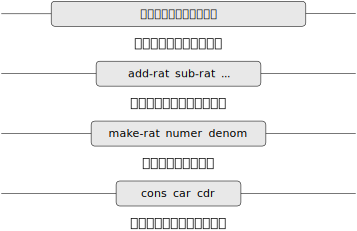
\includegraphics[width=91mm]{fig/chap2/Fig2.1c.pdf}
\par\bigskip
\noindent
\heading{図2.1:} 有理数パッケージ内の抽象化の壁
\end{figure}

例えば、有理数を既約に簡約する問題の別の解き方として、簡約を実行するタイミングを、
有理数の構築時でなく、有理数の部品へのアクセス時にするというやり方があります。
この場合、コンストラクタとセレクタは違ったものになります。

\begin{scheme}
(define (make-rat n d) (cons n d))
(define (numer x)
  (let ((g (gcd (car x) (cdr x))))
    (/ (car x) g)))
(define (denom x)
  (let ((g (gcd (car x) (cdr x))))
    (/ (cdr x) g)))
\end{scheme}

\noindent
この実装と前の実装との違いは、いつ\code{gcd}を計算するかというところです。
プログラムを普通に使う際に、同じ有理数の分子や分母に何回もアクセスするので
あれば、\code{gcd}は有理数の構築時に計算したほうがいいでしょう。そうでなければ、
\code{gcd}の計算はアクセス時まで遅らせたほうがいいかもしれません。どちらを
選ぶにしても、実装を切り替える場合に、\code{add\-/rat}, \code{sub\-/rat}などは
まったく修正する必要がありません。

表現方法への依存を少しだけのインターフェイス手続きに限定することは、
プログラムの修正時だけでなく、プログラムの設計時にも役に立ちます。
そうしておくと、別の実装を考慮するための柔軟性を維持できるからです。
上の単純な例を引き続き使って、有理数パッケージを設計するにあたって、
\code{gcd}を実行するタイミングを構築時にするか選択時にするかを最初の段階で
決められないとします。この場合、データ抽象化という方法を使うことによって、その決定を
後回しにしつつ、システムのほかの部分の開発を進めるということができるようになります。

\begin{quote}
\heading{\phantomsection\label{練習問題 2.2}練習問題 2.2:} 平面上の線分を
表現するという問題について考える。それぞれの線分は、始点と終点という点のペア
として表す。コンストラクタ\code{make\-/segment}とセレクタ\code{start\-/segment},
\code{end\-/segment}を定義せよ。
さらに、点は\( x \)座標と\( y \)座標という数値のペアとして表現できる。
最後に、定義したセレクタとコンストラクタによって、線分を引数として取り
その中点(両端点の座標を平均した座標を持つ点)を返す\code{midpoint\-/segment}
手続きを定義せよ。手続きをチェックするためには、例えば次のようにして
点を表示することが必要となるだろう。

\begin{scheme}
(define (print-point p)
  (newline)
  (display "(")
  (display (x-point p))
  (display ",")
  (display (y-point p))
  (display ")"))
\end{scheme}
\end{quote}

\begin{quote}
\heading{\phantomsection\label{練習問題 2.3}練習問題 2.3:} 平面上の長方形の
表現を実装せよ(ヒント:\link{練習問題 2.2}を利用するといいかもしれない)。
そのコンストラクタとセレクタを使って、ある長方形の外周の長さと面積を計算する
手続きを書け。次に、長方形の異なる表現を実装せよ。適切な抽象化の壁を使って
システムを設計し、外周と面積を求める同じ手続きがどちらの表現によっても動く
ようにできるだろうか。

\end{quote}

\subsection{データとは何か}
\label{2.1.3節}

\link{2.1.1節}での有理数の実装では、有理数演算\code{add\-/rat}, \code{sub\-/rat}
等を、\code{make\-/rat}, \code{numer}, \code{denom}という仕様の決まっていない三つの
手続きによって実装することから始めました。その時点では、それらの演算は
データオブジェクト---分子、分母、有理数---によって定義され、
データオブジェクトのふるまいは後者の三つの手続きによって規定されると
考えることができました。

しかし、\jnewterm{データ}(\newterm{data})とは正確には何を意味しているのでしょうか。
``あるセレクタとコンストラクタによって実装される何か''と言うだけでは十分では
ありません。明らかに、任意の3つの手続きのセットがすべて有理数の実装に対する
適切な基礎としての役割を果たせるわけではありません。有理数\code{x}を\code{n}と\code{d}
という整数のペアによって構築する場合、\code{x}の\code{numer}と\code{denom}を取り出して
割り算を行ったものが、\code{n}を\code{d}で割るのと同じ結果になるということを保証する
必要があります。別の言い方をすると、\code{make\-/rat}, \code{numer}, \code{denom}は、
任意の整数\code{n}とゼロでない整数\code{d}に対し、\code{x}が\code{(make\-/rat n d)}で
あるとき、次の条件を満たす必要があります。
\begin{comment}

\begin{example}
(numer x)    n
--------- = ---
(denom x)    d
\end{example}

\end{comment}
\begin{displaymath}
 {\hbox{\tt(numer x)} \over \hbox{\tt(denom x)}} = {{\tt n} \over {\tt d}}\,.  
\end{displaymath}

実際のところ、これは\code{make\-/rat}, \code{numer}, \code{denom}が有理数表現の
基礎となるために満たさないといけないただひとつの条件です。一般的に、データという
ものは、何らかのセレクタとコンストラクタの集合に加え、それらが有効な表現となるために
満たさなければならないと規定された条件によって定義されるものと考えることができます。
\footnote{意外なことに、この考え方は厳密に定式化することが非常に難しいものです。
そのような定式化には二つのアプローチがあります。ひとつはC. A. R. \link{Hoare (1972)}
が開拓したもので、\jnewterm{抽象モデル}(\newterm{abstract model})という手法として
知られています。この手法では、上の有理数の例で要点を述べた``手続きと条件''という
仕様を定式化するものです。有理数表現での条件は整数に関する事実(等価性と割り算)
によって記述されています。一般的に、抽象モデルではそれまでに定義されたデータ
オブジェクトの型によって新しい種類のデータオブジェクトを定義します。そのため、
データオブジェクトに関する表明は、それまでに定義済みのデータオブジェクトに関する
表明に書き換えてチェックできます。もうひとつのアプローチは、
\acronym{MIT}のZillesと\acronym{IBM}のGoguen, Thatcher, Wagner, Wright
(\link{Thatcher et al. 1978}参照)や、トロント大学のGuttag(\link{Guttag 1977}参照)
によって導入されたもので、\jnewterm{代数的仕様}(\newterm{algebraic specification})
と呼ばれます。代数的仕様では、``手続き''を抽象代数システムの要素と見なし、
そのふるまいは、ここでの``条件''に相当する公理によって規定されるとし、
データオブジェクトに関する表明には抽象代数の技法を使います。どちらの技法も、
\link{Liskov and Zilles (1975)}で調査されています。}

この見方は、有理数のような``高レベル''のデータオブジェクトを定義する場合だけでなく、
低レベルなオブジェクトに対しても使えます。有理数の定義する際に使った、ペアという
概念について考えてみましょう。ペアとは何かということについてはこれまで触れず、
言語がペアを操作する手続きとして\code{cons}, \code{car}, \code{cdr}を用意して
くれているということだけを述べてきました。しかし、これら三つの操作について
知らなければいけないことは、二つのオブジェクトを\code{cons}によってくっつけたら、
それらのオブジェクトを\code{car}と\code{cdr}によって取得できるということだけです。
つまり、それらの操作は、任意のオブジェクト\code{x}と\code{y}に対して、
もし\code{z}が\code{(cons x y)}であるなら\code{(car z)}は\code{x}であり、
\code{(cdr z)}は\code{y}であるという条件を満たすということです。
これら三つの手続きが私たちの言語に基本要素として含まれるということについては
すでに触れたとおりですが、上の条件を満たすものであれば、どんな三つの手続きで
あってもペアを実装する基礎として使うことができます。このことは、
\code{cons}, \code{car}, \code{cdr}を実装するときに、何のデータ構造も使わず、
手続きだけによって行うことができるという事実が鮮やかに示してくれます。
以下はその定義です。

\begin{scheme}
(define (cons x y)
  (define (dispatch m)
    (cond ((= m 0) x)
          ((= m 1) y)
          (else (error "Argument not 0 or 1: CONS" m))))
  dispatch)
(define (car z) (z 0))
(define (cdr z) (z 1))
\end{scheme}

\noindent
このような手続きの使い方は、データというものがどういうものかという私たちの
直感的な概念とまったく対応していません。それでも、これらの手続きが上の
条件を満たすということさえ確認できれば、これがペアを表現する有効なやり方である
ということが示せます。

ここで注意すべき微妙なところは、\code{(cons x y)}に返される値は手続き---
具体的には、内部で定義された手続き\code{dispatch}---だということです。
\code{dispatch}は、ひとつの引数を取り、その引数が0か1かによって
\code{x}か\code{y}かを返します。それに対応して、\code{(car z)}は\code{z}に
0を適用するように定義されています。よって、もし\code{z}が\code{(cons x y)}に
よって作られた手続きであれば、\code{z}を0に適用すると\code{x}を返します。
こうして、\code{(car (cons x y))}が期待通り\code{x}を返すということが示せました。
同様に、\code{(cdr (cons x y))}は\code{(cons x y)}の返り値となる手続きを1に適用し、
\code{y}を返します。このため、この手続きによるペアの実装は有効な実装であり、
\code{cons}, \code{car}, \code{cdr}だけを使ってペアにアクセスするのであれば、
この実装を``本物の''データ構造を使う実装と区別することはできません。

手続きによるペアの実装の実例を示したことのポイントは、私たちの言語がこういうふうに
動いているというわけではなく(Schemeを含め、Lispシステムは一般的に、効率上の理由から
ペアを直接的に実装しています)、こういうふうに動くこともできるということです。
手続きによる表現はわかりにくいですが、ペアが満たす必要のある条件を満たしているため、
ペアを表現する完全に適切な方法と言えます。ここでの例は、手続きをオブジェクトとして
操作する能力は、自動的に複合データを表現する能力を提供するということも示しています。
これは、今の段階ではただの面白い考え方のように思えるかもしれませんが、手続きによる
データの表現というものは、私たちのプログラミングのレパートリーの中で中心的な役割を
果たしています。このプログラミングスタイルはよく\jnewterm{メッセージパッシング}
(\newterm{message passing})と呼ばれ、\link{第3章}でモデル化と
シミュレーションの問題を扱う際には、これを基本的な道具として使うことになります。

\begin{quote}
\heading{\phantomsection\label{練習問題 2.4}練習問題 2.4:}
次に示すものは、手続きによるペアの表現の別のやり方である。この表現で、
任意のオブジェクト\code{x}と\code{y}に対して、\code{(car (cons x y))}が
\code{x}を返すことを確認せよ。

\begin{scheme}
(define (cons x y)
  (lambda (m) (m x y)))
(define (car z)
  (z (lambda (p q) p)))
\end{scheme}

対応する\code{cdr}の定義はどうなるだろうか。(ヒント:これが動作することを
確認するには\link{1.1.5節}の置換モデルを利用する)
\end{quote}

\begin{quote}
\heading{\phantomsection\label{練習問題 2.5}練習問題 2.5:}
\( a \)と\( b \)のペアを積\( 2^a 3^b \)の整数で表現することによって、
非負整数のペアを数値と数値演算だけを使って表現できるということを示せ。

それに対応する\code{cons}, \code{car}, \code{cdr}手続きを定義せよ。
\end{quote}

\begin{quote}
\heading{\phantomsection\label{練習問題 2.6}練習問題 2.6:}
ペアを手続きとして表現するという考え方で頭がごちゃごちゃになっていないとしたら、
次のようなことを考えてみよう。手続きを扱うことができる言語では、
(少なくとも、非負整数に関する限りは)数値なしでもやっていける。
そのためには、0と、1を足すという演算を次のように実装する。

\begin{scheme}
(define zero (lambda (f) (lambda (x) x)))
(define (add-1 n)
  (lambda (f) (lambda (x) (f ((n f) x)))))
\end{scheme}

この表現は、発明者のAlonzo Churchにちなんで\jnewterm{チャーチ数}
(\newterm{Church numeral})として知られている。Alonzo Churchは
\( \lambda \)-演算を発明した論理学者である。

\code{one}と\code{two}を直接(\code{zero}と\code{add\-/1}を使わずに)定義せよ
(ヒント:置換を使って\code{(add\-/1 zero)}を評価する)。
加算手続きの直接的な定義\code{+}(\code{add\-/1}の繰り返し適用は用いない)を与えよ。
\end{quote}


\subsection{発展問題: 区間演算}
\label{2.1.4節}

Alyssa P. Hackerは工学上の問題の解決を助けるシステムを設計しています。
システムで提供したい機能のひとつとして、精度のわかっている不正確な量
(例えば物理装置の測定値)を扱う能力があります。そのような近似値を使って
計算を行った場合、結果が精度つきの数値となるようにしたいということです。

電気技師はAlyssaのシステムを使って電気に関するいろいろな値を計算します。
その際に、二つの抵抗\( R_1 \), \( R_2 \)の並列に等価な抵抗値\( R_p \)
を次の式によって計算することが必要になるときがあります。

\begin{comment}

\begin{example}
            1
R_p = -------------
      1/R_1 + 1/R_2
\end{example}

\end{comment}
\begin{displaymath}
 R_p = {1 \over 1 / R_1 + 1 / R_2}.  
\end{displaymath}
抵抗値は普通、抵抗の製造者によって保証された何らかの許容誤差の範囲内であることしか
わかりません。例えば、``10\%の許容誤差で6.8Ω''というラベルのついた抵抗を買うと、
その抵抗の抵抗値は\( 6.8 - 0.68 = 6.12 \)から\( 6.8 + 0.68 = 7.48 \)Ωの間である
ということしか確かには言えません。そのため、6.8Ω 10\%の抵抗と4.7Ω 5\%の抵抗を
並列に接続すると、その組み合わせの抵抗は約2.58Ω(二つの抵抗が下限値である場合)から
約2.97Ω(二つの抵抗が上限値である場合)までの範囲になります。

Alyssaのアイデアは、``区間''(不正確な量の取り得る値の範囲を表すオブジェクト)を
組み合わせる数値演算のセットとして``区間演算''を実装するというものでした。
二つの区間を足し算、引き算、かけ算、割り算した結果は、それ自身が区間であり、
結果の範囲を表します。

Alyssaは、下限と上限という二つの端点を持つ``区間''という抽象オブジェクトがあると
仮定しました。また、区間の両端点が与えられれば、データコンストラクタ
\code{make\-/interval}を使って区間を構築できるとしました。Alyssaはまず、
二つの区間を足す手続きを書きます。彼女は、和が取り得る最小値は二つの下限の和であり、
最大値は二つの上限の和だろうと推論します。

\begin{scheme}
(define (add-interval x y)
  (make-interval (+ (lower-bound x) (lower-bound y))
                 (+ (upper-bound x) (upper-bound y))))
\end{scheme}

\noindent

またAlyssaは、両端点の積の最小値と最大値を求め、それらを答えとなる区間の
下限と上限とすることによって、二つの区間の積を計算しました
(\code{min}と\code{max}は、任意の数の引数の最小値と最大値を見つける基本要素です)。

\begin{scheme}
(define (mul-interval x y)
  (let ((p1 (* (lower-bound x) (lower-bound y)))
        (p2 (* (lower-bound x) (upper-bound y)))
        (p3 (* (upper-bound x) (lower-bound y)))
        (p4 (* (upper-bound x) (upper-bound y))))
    (make-interval (min p1 p2 p3 p4)
                   (max p1 p2 p3 p4))))
\end{scheme}

\noindent
二つの区間の割り算は、一つ目に二つ目の逆数をかけることにします。区間の逆数の
下限と上限は、上限の逆数と下限の逆数という順番になることに気をつけてください。

\begin{scheme}
(define (div-interval x y)
  (mul-interval
   x
   (make-interval (/ 1.0 (upper-bound y))
                  (/ 1.0 (lower-bound y)))))
\end{scheme}

\begin{quote}
\heading{\phantomsection\label{練習問題 2.7}練習問題 2.7:}
区間の抽象化の実装を規定していないため、Alyssaのプログラムは未完成である。
区間のコンストラクタの定義は以下のようになる。

\begin{scheme}
(define (make-interval a b) (cons a b))
\end{scheme}

セレクタ\code{upper\-/bound}と\code{lower\-/bound}を定義し、実装を完成させよ。
\end{quote}

\begin{quote}
\heading{\phantomsection\label{練習問題 2.8}練習問題 2.8:} Alyssaと
同じような推論を使って、二つの区間の差をどのように計算するかを記述せよ。
それに対応する引き算の手続き\code{sub\-/interval}を定義せよ。
\end{quote}

\begin{quote}
\heading{\phantomsection\label{練習問題 2.9}練習問題 2.9:}
区間の\jnewterm{幅}(\newterm{width})は、上限と下限の差の半分である。
幅は、区間によって規定される数値の不確かさの程度である。いくつかの
数値演算では、二つの区間を組み合わせた結果の幅は、引数の区間の幅のみによる
関数となるが、それら以外の演算では、組み合わせたものの幅は、引数の幅の
関数とはならない。二つの区間の和(または差)の幅は、足される(または引かれる)
区間の幅の関数となることを示せ。これが乗算と除算については正しくないということを
例を挙げて示せ。
\end{quote}

\begin{quote}
\heading{\phantomsection\label{練習問題 2.10}練習問題 2.10:} エキスパートシステム
プログラマのBen Bitdiddleは、Alyssaの肩越しにのぞいてきて、長さがゼロの
区間で割るということの意味がはっきりしていないとコメントした。
Alyssaのコードを修正し、この条件についてチェックして、もしこれが起こればエラーの
シグナルを送るようにせよ。
\end{quote}

\begin{quote}
\heading{\phantomsection\label{練習問題 2.11}練習問題 2.11:}
ついでにBenはまた謎めいたコメントを残した。``区間の両端点の符号をテストすると
\code{mul\-/interval}は9パターンに場合分けできて、2回以上のかけ算が必要になるのは
その中のひとつだけだよ。'' Benの提案に従って、この手続きを書き直せ。

\end{quote}
\noindent
プログラムをデバッグしてから、Alyssaはユーザ候補の一人にそれを見せました。
その人は、このプログラムは解いている問題が違う、ほしいのは中央値と
許容誤差で表される数値を扱うプログラムだと言います。例えば、\( 3.5 \pm 0.15 \)の
ような区間を使って作業をしたいのであって、[3.35, 3.65]ではないということです。
Alyssaは自分のデスクに戻って、別のコンストラクタと別のセレクタを提供する
ことによってこの問題を解決しました。

\begin{scheme}
(define (make-center-width c w)
  (make-interval (- c w) (+ c w)))
(define (center i)
  (/ (+ (lower-bound i) (upper-bound i)) 2))
(define (width i)
  (/ (- (upper-bound i) (lower-bound i)) 2))
\end{scheme}
\noindent
運の悪いことに、Alyssaのユーザのほとんどは技師です。実際の工学の現場では、
測定値の誤差は小さなもので、区間の中央値に対する幅の割合として表されます。
技師は普通、上で書いた抵抗のスペックのように、装置のパラメタに対する
パーセント許容誤差を規定するものです。

\begin{quote}
\heading{\phantomsection\label{練習問題 2.12}練習問題 2.12:}
中央値とパーセント許容誤差を取り、求める範囲を返すコンストラクタ
\code{make\-/center\-/percent}を定義せよ。また、与えられた区間に対して
パーセント許容誤差を返すセレクタ\code{percent}も定義する必要がある。
\code{center}セレクタは上に書いたものと同じである。
\end{quote}

\begin{quote}
\heading{\phantomsection\label{練習問題 2.13}練習問題 2.13:}
パーセント許容誤差が小さいという前提のもとでは、二つの区間の積のパーセント許容誤差を
因数の許容誤差の積によって近似する簡単な式が存在することを示せ。
すべての数値は正であると仮定して問題を単純化してもよい。
\end{quote}

\noindent
かなりの作業ののちに、Alyssa P. Hackerは完成したシステムを納品しました。
数年後、そのことをすっかり忘れていたころ、怒り狂ったユーザLem E. Tweakitから
興奮した口調の電話がかかってきました。どうもLemは、並列抵抗の式が
代数的に等価な以下の二つの方法で書けることに気づいたようです。
\begin{comment}

\begin{example}
 R_1 R_2
---------
R_1 + R_2
\end{example}

\end{comment}
\begin{displaymath}
 R_1 R_2 \over R_1 + R_2 
\end{displaymath}
\noindent

\begin{comment}

\begin{example}
      1
-------------
1/R_1 + 1/R_2
\end{example}

\end{comment}
\begin{displaymath}
 {1 \over 1 / R_1 + 1 / R_2}. 
\end{displaymath}
彼は次の二つのプログラムを書きました。それぞれ、並列抵抗の式を異なったやり方で計算します。

\begin{scheme}
(define (par1 r1 r2)
  (div-interval (mul-interval r1 r2)
                (add-interval r1 r2)))
\end{scheme}

\begin{scheme}
(define (par2 r1 r2)
  (let ((one (make-interval 1 1)))
    (div-interval
     one (add-interval (div-interval one r1)
                       (div-interval one r2)))))
\end{scheme}

\vspace{0.3em}

Lemは、Alyssaのプログラムがこれら二つの計算方法に対して異なる値を返すと苦情を言っています。
これは深刻な苦情です。

\begin{quote}
\heading{\phantomsection\label{練習問題 2.14}練習問題 2.14:}
Lemが正しいことを示せ。いろいろな数値演算の式についてこのシステムの挙動を
調査せよ。何らかの区間\( A \)と\( B \)を作成し、それらを使って
式\( A / A \)と\( A / B \)を計算せよ。中央値に対して小さなパーセンテージの幅を
持つ区間について調べると得られるところが大きいだろう。中央値-パーセント形式
(\link{練習問題 2.12}参照)の計算結果を調べよ。
\end{quote}

\begin{quote}
\heading{\phantomsection\label{練習問題 2.15}練習問題 2.15:}
別のユーザEva Lu Atorも、代数的に等価な異なる式によって計算すると
異なる区間になることに気がついた。彼女は、不確定な数値を表す変数が
繰り返し出てこないように書けば、より厳密な誤差限界を返すようにできると言う。
つまり、並列抵抗を計算するのに\code{par2}は\code{par1}よりも``よりよい''
プログラムだと言うのだ。彼女は正しいだろうか。また、それはなぜだろうか。
\end{quote}

\begin{quote}
\heading{\phantomsection\label{練習問題 2.16}練習問題 2.16:}
一般的に、なぜ代数的に等価な式が異なる答えになることがあるのかを説明せよ。
この欠点のない区間演算パッケージを開発することはできるだろうか。
それとも、このタスクは不可能なのだろうか。(警告:この問題はとても難しい)
\end{quote}

%=======================================================================================================

\section{階層データと閉包性}
\label{2.2節}

ここまでで見てきたように、ペアは私たちが複合データオブジェクトを構築する
基本的な``糊''となってくれます。\link{図2.2}は、ペア---この場合は
\code{(cons 1 2)}で作られるペア---を図示する標準的なやり方を示しています。
この表現は\jnewterm{箱とポインタ記法}(\newterm{box-and-pointer notation})と
呼ばれるもので、それぞれのオブジェクトは箱への\jnewterm{ポインタ}
(\newterm{pointer})として表わされます。基本オブジェクトの箱には
オブジェクトの表現が入っています。例えば、数値の箱には数字が入っています。
ペアの箱は実際には二つの箱で、左の箱にはペアの\code{car}(へのポインタ)
が入り、右の箱には\code{cdr}が入ります。

\code{cons}は、数値だけでなくペアも結合できるということについてはすでに見ました
(\link{練習問題 2.2}と\link{練習問題 2.3}を解く際には、この事実を使ったはずです)。
結果として、ペアはどんな種類のデータ構造でも
構築できる汎用ブロックとなってくれます。\link{図2.3}は
ペアを使って数値1, 2, 3, 4を組み合わせる二つの方法を示しています。

\begin{figure}[tb]
\phantomsection\label{図2.2}
\centering
\begin{comment}
\heading{図2.2:} Box-and-pointer representation of \code{(cons 1 2)}.

\begin{example}
     +---+---+     +---+
---->| * | *-+---->| 2 |
     +-|-+---+     +---+
       |
       V
     +---+
     | 1 |
     +---+
\end{example}
\end{comment}
\includegraphics[width=34mm]{fig/chap2/Fig2.2c.pdf}
\par\bigskip
\noindent
\heading{図2.2:} \code{(cons 1 2)}の箱とポインタ表現
\end{figure}

\begin{figure}[tb]
\phantomsection\label{図2.3}
\centering
\begin{comment}
\heading{図2.3:} Two ways to combine 1, 2, 3, and 4 using pairs.

\begin{example}
     +---+---+     +---+---+         +---+---+     +---+
---->| * | *-+---->| * | * |    ---->| * | *-+---->| 4 |
     +-|-+---+     +-|-+-|-+         +-|-+---+     +---+
       |             |   |             |
       V             V   V             V
   +---+---+      +---+ +---+      +---+---+     +---+---+
   | * | * |      | 3 | | 4 |      | * | *-+---->| * | * |
   +-|-+-|-+      +---+ +---+      +-|-+---+     +-|-+-|-+
     |   |                           |             |   |
     V   V                           V             V   V
  +---+ +---+                      +---+        +---+ +---+
  | 1 | | 2 |                      | 1 |        | 2 | | 3 |
  +---+ +---+                      +---+        +---+ +---+

  (cons (cons 1 2)                 (cons (cons 1
        (cons 3 4))                            (cons 2 3))
                                         4)
\end{example}
\end{comment}
\includegraphics[width=96mm]{fig/chap2/Fig2.3c.pdf}
\begin{quote}
\heading{図2.3:} ペアを使って1, 2, 3, 4を組み合わせる二つの方法
\end{quote}
\end{figure}

ペアを要素とするペアを作る能力は、表現ツールとしてのリスト構造の持つ重要性の
本質となるものです。この能力のことを、\code{cons}の\jnewterm{閉包性}
(\newterm{closure property})と呼びます。一般的に、データオブジェクトを組み合わせる操作は、
その演算による組み合わせの結果自身が同じ演算によって組み合わせることができるので
あれば、閉包性を満たします。
\footnote{
ここでの``閉包''という言葉は抽象代数から来ています。
抽象代数では、集合の要素に演算を適用して得られるものがまたその集合の要素であるなら、
それらの要素の集合はその演算のもとで閉じていると言います。ところで、Lispコミュニティでは、
(不幸なことに)``閉包''という言葉をまったく関係のない別の概念の記述にも使っています。
その場合の閉包とは、自由変数を持つ手続きを表現する実装上のテクニックを
指しています。この本では、そちらの意味での``閉包''は使いません。}
閉包は、どんな組み合わせ手段であっても、表現力の鍵となるものです。それによって、
\jnewterm{階層}(\newterm{hierarchical})構造---部品によって作られ、その部品も
また部品によって作られ\( \dots \)という構造---を作ることが可能になるからです。

\link{第1章}の初めから、手続きを扱う際には本質的に閉包を使ってきました。
とても単純なプログラム以外は、組み合わせの要素はそれ自身組み合わせとなりうる
という事実に依存しているからです。この節では、複合データの閉包がもたらす結果に
ついて扱います。また、ペアを使って列や木を表現するいくつかの確立されたテクニックに
ついて説明し、閉包を鮮やかに形にしてくれるグラフィック言語を紹介します。
\footnote{
組み合わせ手段は閉包性を満たすべきだという概念は素直な考え方です。残念なことに、
一般的に使われる言語の多くでは、データ結合手段として提供されているものが
閉包性を満たさなかったり、閉包を使うのが面倒だったりします。FortranやBASICでは、
普通は配列にまとめて入れることでデータを組み合わせます。しかし、要素がそれ自身
配列であるような配列は作れません。PascalとCでは、要素が構造体であるような
構造体を認めています。しかし、これをするためにはプログラマが明示的にポインタを
扱わなければならず、またプログラマは構造体の各フィールドが前もって決められた形の
要素しか持つことができないという制約に従わなければなりません。これらの言語は、
Lispがペアとして提供しているような、複合データを統一的な方法で簡単に操作できる
ビルトインの汎用の糊を持っていません。この制約が、Alan Perlisがこの本の前書きで
コメントしたことの背景にあります。``Pascalでは、宣言可能なデータ構造の多さが
関数の専門化を引き起こし、気軽な連携は禁じられ、ペナルティを与えられるものとなります。
ひとつのデータ構造を扱う100の関数があるほうが、10のデータ構造を扱う10の関数が
あるのよりもよいのです。''}

\subsection{列の表現}
\label{2.2.1節}

ペアを使って構築できる便利な構造のひとつは、\jnewterm{列}(\newterm{sequence})---
データオブジェクトの順序つき集合---です。もちろん、ペアを使って列を表すやり方は
いろいろあります。\link{図2.4}には、特に素直な表現方法のひとつを示しています。
このやり方では、1, 2, 3, 4という列はペアのチェーンとして表されます。それぞれのペアの
\code{car}はチェーン内の対応する項で、ペアの\code{cdr}はチェーン内の次のペアです。
最後のペアの\code{cdr}は、ペアでない特別な値を指すことによって、列の終端である
ことを伝えます。その値は、箱-ポインタ図では斜線として表され、プログラムでは
変数\code{nil}という値として表されます。列全体は、入れ子の\code{cons}演算によって
構築されます。

\begin{scheme}
(cons 1
      (cons 2
            (cons 3
                  (cons 4 nil))))
\end{scheme}

\begin{figure}[tb]
\phantomsection\label{図2.4}
\centering
\begin{comment}
\heading{図2.4:} The sequence 1, 2, 3, 4 represented as a chain of pairs.

\begin{example}
     +---+---+     +---+---+     +---+---+     +---+---+
---->| * | *-+---->| * | *-+---->| * | *-+---->| * | / |
     +-|-+---+     +-|-+---+     +-|-+---+     +-|-+---+
       |             |             |             |
       V             V             V             V
     +---+         +---+         +---+         +---+
     | 1 |         | 2 |         | 3 |         | 4 |
     +---+         +---+         +---+         +---+
\end{example}
\end{comment}
\includegraphics[width=76mm]{fig/chap2/Fig2.4c.pdf}
\par\bigskip
\noindent
\heading{図2.4:} ペアの鎖として表現された列1, 2, 3, 4
\end{figure}

入れ子の\code{cons}によって作られるこのようなペアの列は\jnewterm{リスト}
(\newterm{list})と呼ばれます。Schemeは、リスト構築を便利にする
\code{list}という基本手続きを提供しています。
\footnote{この本では、\jnewterm{リスト}(\newterm{list})という言葉はリスト終端
マーカーで終わるペアのチェーンという意味で使います。それに対して、
\jnewterm{リスト構造}(\newterm{list structure})という用語は、リストに限らず、
ペアによって作られた任意のデータ構造を指します。}
上の列は、\code{(list 1 2 3 4)}によって生成できます。
一般的に、

\begin{scheme}
(list ~\( \dark \langle \)~~\( \dark a_1 \)~~\( \dark \rangle \)~ ~\( \dark \langle \)~~\( \dark a_2 \)~~\( \dark \rangle \)~ ~\( \dots \)~ ~\( \dark \langle \)~~\( \dark a_n \)~~\( \dark \rangle \)~)
\end{scheme}

\noindent
は次のものと等価です。

\begin{scheme}
(cons ~\( \dark \langle \)~~\( \dark a_1 \)~~\( \dark \rangle \)~
      (cons ~\( \dark \langle \)~~\( \dark a_2 \)~~\( \dark \rangle \)~
            (cons ~\( \dots \)~
                  (cons ~\( \dark \langle \)~~\( \dark a_n \)~~\( \dark \rangle \)~
                        nil)~\( \dots \)~)))
\end{scheme}

\noindent
Lispシステムは、慣例的にリストを括弧でくくられた要素の列として表示します。
そのため、\link{図2.4}のデータオブジェクトは\code{(1 2 3 4)}と表示されます。

\begin{scheme}
(define one-through-four (list 1 2 3 4))
one-through-four
~\textit{(1 2 3 4)}~
\end{scheme}

\noindent
式\code{(list 1 2 3 4)}と、その式を評価した結果として得られるリスト
\mbox{\code{(1 2 3 4)}}を混同しないように気をつけてください。
式\code{(1 2 3 4)}を評価しようとすると、インタプリタは手続き\code{1}を
引数\code{2}, \code{3}, \code{4}に適用しようとして、エラーを起こします。

\code{car}はリストの最初の項を選択し、\code{cdr}は最初の項以外のすべてからなる
サブリストを選択するものであると考えることもできます。
\code{car}と\code{cdr}を入れ子で適用していくと、リストの二つ目、三つ目、それから
それに続く項を取り出すことができます。\footnote{
\code{car}と\code{cdr}の入れ子適用は書くのが面倒なので、Lispの諸方言はそれらの
省略形を提供しています。例えば、

\begin{smallscheme}
(cadr ~\( \dark \langle \)~~\( \dark ar\!g \)~~\( \dark \rangle \)~) = (car (cdr ~\( \dark \langle \)~~\( \dark arg \)~~\( \dark \rangle \)~))
\end{smallscheme}

このような手続きの名前はすべて\code{c}で始まり\code{r}で終わります。間の\code{a}は
\code{car}演算を表し、\code{d}は\code{cdr}演算を表し、名前の中での順番と同じ順番で
適用されます。\code{cadr}のような単純な組み合わせが発音可能になるように、
\code{car}と\code{cdr}の名前を残しています。}
コンストラクタ\code{cons}は、元のリストと同じリストに最初にひとつ項が加わったものを
作ります。

\begin{scheme}
(car one-through-four)
~\textit{1}~
(cdr one-through-four)
~\textit{(2 3 4)}~
(car (cdr one-through-four))
~\textit{2}~
(cons 10 one-through-four)
~\textit{(10 1 2 3 4)}~
(cons 5 one-through-four)
~\textit{(5 1 2 3 4)}~
\end{scheme}

\noindent
\code{nil}という値はペアのチェーンを終了させるために使うものですが、これを
要素のない列\jnewterm{空リスト}(\newterm{empty list})と考えることもできます。
\newterm{nil}という単語は、``無''を意味するラテン語の単語\emph{nihil}を短くした
ものです。
\footnote{Lispの諸方言の標準化にあたって、どれだけのエネルギーが文字通り
無に消えたかというのは特筆すべきことです。\code{nil}は普通の名前であるべきか、
 \code{nil}の値は記号であるべきか、リストであるべきか、ペアであるべきか、といったものです。
Schemeでは\code{nil}は普通の名前で、この節では値がリスト終端マーカーであるような
変数として使います(\code{true}が真の値を持つ普通の変数であるのと同じです)。
Common LispなどのLisp方言では、\code{nil}を特別な記号として扱います。
この本の著者たちは言語標準化で多くの争いを経験してきたので、この問題そのものを
避けたいと思っています。\link{2.3節}でクォートを導入したら、空リストを
\code{'()}として示し、完全に変数\code{nil}を使わないですむようにします。}

\subsubsection*{リスト演算}

ペアを使って要素の列をリストとして表現するやり方は、リストを
``\code{cdr}ダウン''していくという確立されたプログラミングテクニックと
セットになっています。例えば、\code{list\-/ref}手続きは引数として
リストと数値\( n \)を取り、リストの\( n \)番目のものを返します。
リストの要素の番号は0から始めるのが慣例となっています。
\code{list\-/ref}を計算する方法は以下の通りです。

\begin{itemize}

\item
\( n = 0 \)であれば、\code{list\-/ref}はリストの\code{car}を返す。

\item
そうでなければ、\code{list\-/ref}はリストの\code{cdr}の\( (n - 1) \)番目のものを返す。

\end{itemize}

\begin{scheme}
(define (list-ref items n)
  (if (= n 0)
      (car items)
      (list-ref (cdr items) (- n 1))))
(define squares (list 1 4 9 16 25))
(list-ref squares 3)
~\textit{16}~
\end{scheme}

\noindent
リスト全体を\code{cdr}ダウンすることもよくあります。それをやりやすくするために
Schemeは基本述語\code{null?}を持っています。これは、引数が空リストかどうか
テストするものです。\code{length}というリストの要素数を返す手続きは、
その典型的な使用パターンを示しています。

\begin{scheme}
(define (length items)
  (if (null? items)
      0
      (+ 1 (length (cdr items)))))
(define odds (list 1 3 5 7))
(length odds)
~\textit{4}~
\end{scheme}

\noindent
手続き\code{length}は、単純な再帰計画を実装しています。簡約ステップは以下の通りです。

\begin{itemize}

\item
任意のリストの\code{length}は、リストの\code{cdr}の\code{length}に1を足した値である。

\end{itemize}

\noindent
これは、次の基本ケースに着くまで連続的に適用されます。

\begin{itemize}

\item
空リストの\code{length}は0である。

\end{itemize}

\noindent
\code{length}は、反復スタイルで計算することもできます。

\begin{scheme}
(define (length items)
  (define (length-iter a count)
    (if (null? a)
        count
        (length-iter (cdr a) (+ 1 count))))
  (length-iter items 0))
\end{scheme}

\noindent
もうひとつの確立されたプログラミングテクニックは、リストを\code{cdr}ダウンしながら
答えのリストを``\code{cons}アップ''するというものです。これは、次の\code{append}
手続きで使われます。\code{append}手続きは、二つのリストを引数として取り、
要素を連結して新しいリストを作ります。

\begin{scheme}
(append squares odds)
~\textit{(1 4 9 16 25 1 3 5 7)}~
(append odds squares)
~\textit{(1 3 5 7 1 4 9 16 25)}~
\end{scheme}

\noindent
\code{append}も再帰計画を使って実装されています。
リスト\code{list1}と\code{list2}を\code{append}するには、次のようにします。

\begin{itemize}

\item
もし\code{list1}が空リストであれば、結果は単に\code{list2}である。

\item
そうでなければ、\code{list1}の\code{cdr}と\code{list2}を\code{append}し、その結果に
\code{list1}の\code{car}を\code{cons}する。

\end{itemize}

\begin{scheme}
(define (append list1 list2)
  (if (null? list1)
      list2
      (cons (car list1) (append (cdr list1) list2))))
\end{scheme}

\begin{quote}
\heading{\phantomsection\label{練習問題 2.17}練習問題 2.17:} 与えられた(空でない)
リストの最後の要素のみを持つリストを返す手続き\code{last\-/pair}を定義せよ。

\begin{scheme}
(last-pair (list 23 72 149 34))
~\textit{(34)}~
\end{scheme}
\end{quote}

\begin{quote}
\heading{\phantomsection\label{練習問題 2.18}練習問題 2.18:}リストを引数として取り、
同じ要素を逆順に持つリストを返す手続き\code{reverse}を定義せよ。

\begin{scheme}
(reverse (list 1 4 9 16 25))
~\textit{(25 16 9 4 1)}~
\end{scheme}
\end{quote}

\begin{quote}
\heading{\phantomsection\label{練習問題 2.19}練習問題 2.19:}
\link{1.2.2節}の両替パターン数計算プログラムについて考える。
プログラムで使う通貨を変えられるようにして、例えばイギリスポンドの両替パターン数を
計算できるようになると便利だろう。現状のプログラムでは、通貨についての知識は
一部は\code{first\-/denomination}に、一部は\code{count\-/change}
(アメリカには5種類のコインがあるということを知っている)に分散されている。
両替に使うコインのリストを与えられるようになればもっとよくなるだろう。

手続き\code{cc}を書き直して、二つ目の引数として取るものを、どのコインを使うかを
指定する整数ではなく、使うコインの値のリストとなるようにしたい。それから、
それぞれの通貨の種類を定義するリストを次のように持っておく。

\begin{scheme}
(define us-coins (list 50 25 10 5 1))
(define uk-coins (list 100 50 20 10 5 2 1 0.5))
\end{scheme}

そして、\code{cc}は次のように呼び出すことにしよう。

\begin{scheme}
(cc 100 us-coins)
~\textit{292}~
\end{scheme}

このためには、プログラム\code{cc}に対して何らかの変更を加える必要がある。
プログラムの形は同じだが、二つ目の引数に対するアクセスの仕方が次のように
変わる。

\begin{scheme}
(define (cc amount coin-values)
  (cond ((= amount 0) 1)
        ((or (< amount 0) (no-more? coin-values)) 0)
        (else
         (+ (cc amount
                (except-first-denomination
                 coin-values))
            (cc (- amount
                   (first-denomination
                    coin-values))
                coin-values)))))
\end{scheme}

リスト構造に対する基本演算によって、手続き\code{first\-/denomination},
\code{except\-/first\-/denomination}, \code{no\-/more?}を定義せよ。
リスト\code{coin\-/values}の順序は、\code{cc}によって返される解答に影響を与える
だろうか、それとも与えないだろうか。それはどうしてだろうか。
\end{quote}

\begin{quote}
\heading{\phantomsection\label{練習問題 2.20}練習問題 2.20:}
手続き\code{+}, \code{*}, \code{list}は任意の数の引数を取る。このような手続きを定義する
方法のひとつとして、\code{define}で\jnewterm{ドット末尾記法}
(\newterm{dotted-tail notation})を使うというものがある。手続きの定義の中で、
仮引数リストの最後の仮引数名の前にドットのあるものは、手続きが呼ばれるときに、
前のほうの仮引数は(もしあれば)通常通り前のほうの引数の値を持つことになるが、
最後の仮引数の値は残りの引数すべての\jnewterm{リスト}(\newterm{list})となる。
例えば、次のような定義の場合、

\begin{scheme}
(define (f x y . z) ~\( \dark \langle \)~~\var{\dark body}~~\( \dark \rangle \)~)
\end{scheme}

\noindent
手続き\code{f}は、二つ以上の引数で呼び出すことができる。次のものを評価すると、

\begin{scheme}
(f 1 2 3 4 5 6)
\end{scheme}

\noindent
\code{f}の本体では、\code{x}は1となり、\code{y}は2で、\code{z}はリスト\mbox{\code{(3 4 5 6)}}となる。
次の定義の場合、

\begin{scheme}
(define (g . w) ~\( \dark \langle \)~~\var{\dark body}~~\( \dark \rangle \)~)
\end{scheme}

\noindent
手続き\code{g}は0個以上の引数で呼び出すことができる。次のものを評価すると、

\begin{scheme}
(g 1 2 3 4 5 6)
\end{scheme}

\noindent
\code{g}の本体では、\code{w}はリスト\code{(1 2 3 4 5 6)}となる。
\footnote{
\code{lambda}を使って\code{f}と\code{g}を定義する場合、次のように書けます。

\begin{smallscheme}
(define f (lambda (x y . z) ~\( \dark \langle \)~~\var{\dark body}~~\( \dark \rangle \)~))
(define g (lambda w ~\( \dark \langle \)~~\var{\dark body}~~\( \dark \rangle \)~))
\end{smallscheme}
}

\code{same\-/parity}は、ひとつ以上の整数を引数として取り、最初の引数と同じ
偶奇性を持つ引数すべてのリストを返す手続きとする。例えば、次のようになる。

\begin{scheme}
(same-parity 1 2 3 4 5 6 7)
~\textit{(1 3 5 7)}~
(same-parity 2 3 4 5 6 7)
~\textit{(2 4 6)}~
\end{scheme}
\end{quote}

上記の記法を使ってこの手続きを書け。

\subsubsection*{リストに対するマップ}

非常に便利な演算として、リストのそれぞれの要素に何らかの変換を適用し、結果のリストを
返すというものがあります。例えば、次の手続きは与えられた係数をリストのそれぞれの数値に
かけます。

\begin{scheme}
(define (scale-list items factor)
  (if (null? items)
      nil
      (cons (* (car items) factor)
            (scale-list (cdr items)
                        factor))))
(scale-list (list 1 2 3 4 5) 10)
~\textit{(10 20 30 40 50)}~
\end{scheme}

\noindent
\link{1.3節}でやったように、この一般的な考え方を抽象化し、高階手続きによって
表現される共通パターンとして捉えることができます。ここでの高階手続きは、
\code{map}と呼ばれるものです。\code{map}は、1引数の手続きとリストを引数として取り、
リストのそれぞれの要素に手続きを適用した結果のリストを返します。
\footnote{\label{Footnote 12}
Schemeは、ここで記述したものよりも汎用的な\code{map}手続きを標準で提供しています。
そのより汎用的な\code{map}は、引数として\( n \)引数の手続きと\( n \)個のリストを取り、
手続きを、すべてのリストの一つ目の要素、すべてのリストの二つ目の要素\( \dots \)に対して
適用していき、結果のリストを返します。例えば、次のようになります。

\begin{smallscheme}
(map + (list 1 2 3) (list 40 50 60) (list 700 800 900))
~\textit{(741 852 963)}~
(map (lambda (x y) (+ x (* 2 y)))
     (list 1 2 3)
     (list 4 5 6))
~\textit{(9 12 15)}~
\end{smallscheme}
}

\begin{scheme}
(define (map proc items)
  (if (null? items)
      nil
      (cons (proc (car items))
            (map proc (cdr items)))))
(map abs (list -10 2.5 -11.6 17))
~\textit{(10 2.5 11.6 17)}~
(map (lambda (x) (* x x)) (list 1 2 3 4))
~\textit{(1 4 9 16)}~
\end{scheme}

\noindent
これで、\code{map}を使って\code{scale\-/list}の新しい定義を書くことができます。

\begin{scheme}
(define (scale-list items factor)
  (map (lambda (x) (* x factor))
       items))
\end{scheme}

\noindent
\code{map}は重要な概念ですが、それは\code{map}が共通パターンを捉えているという理由から
だけではありません。\code{map}はリストを扱ううえでのより高いレベルの抽象化を達成するからです。
元の\code{scale\-/list}の定義では、プログラムは再帰構造になっていて、リストの
要素ごとの処理に注意が向くようになっていました。\code{map}によって\code{scale\-/list}を
定義すると、そのレベルの細かいことは隠されて、係数倍というものが要素のリストを結果の
リストに変換するものであるというところが強調されます。二つの定義の違いは、コンピュータが
実行するプロセスの違いではなく(プロセスは同じものです)、私たちがプロセスをどう捉えるかという
違いです。実際に\code{map}は、リストを変形する手続きの
実装を、リストの要素をどうやって取り出して結合していくかという細かいところから切り離す
抽象化の壁を作ることを助けてくれます。\link{図2.1}で示した壁のように、
この抽象化を使うことで、列を列に変形するという概念的な演算の枠組みを保ったままで、
列の実装方法という低レベルな詳細を変更できる柔軟性が得られます。
\link{2.2.3節}では、列をプログラム組織化の枠組みとするというこの使い方についてさらに詳しく
説明します。

\begin{quote}
\heading{\phantomsection\label{練習問題 2.21}練習問題 2.21:}
手続き\code{square\-/list}は、引数として数値のリストを取り、それらの数値の二乗の列を
持つリストを返す。

\begin{scheme}
(square-list (list 1 2 3 4))
~\textit{(1 4 9 16)}~
\end{scheme}

次に二つの異なる\code{square\-/list}の定義を示す。書けた部分を埋め、二つとも完成させよ。

\begin{scheme}
(define (square-list items)
  (if (null? items)
      nil
      (cons ~\( \dark \langle \)~??~\( \dark \rangle \)~ ~\( \dark \langle \)~??~\( \dark \rangle \)~)))
(define (square-list items)
  (map ~\( \dark \langle \)~??~\( \dark \rangle \)~ ~\( \dark \langle \)~??~\( \dark \rangle \)~))
\end{scheme}
\end{quote}

\begin{quote}
\heading{\phantomsection\label{練習問題 2.22}練習問題 2.22:}
Louis Reasonerは\link{練習問題 2.21}の一つ目の\code{square\-/list}手続きを書き直し、
反復プロセスを展開するようにしようとしている。

\begin{scheme}
(define (square-list items)
  (define (iter things answer)
    (if (null? things)
        answer
        (iter (cdr things)
              (cons (square (car things))
                    answer))))
  (iter items nil))
\end{scheme}

残念ながら、このように\code{square\-/list}を定義すると、答えとなるリストは
望むものの逆順になってしまう。なぜだろうか。

それから、Louisは\code{cons}の引数を逆順にしてバグを直そうとした。

\begin{scheme}
(define (square-list items)
  (define (iter things answer)
    (if (null? things)
        answer
        (iter (cdr things)
              (cons answer
                    (square (car things))))))
  (iter items nil))
\end{scheme}

これもうまくいかない。説明せよ。
\end{quote}

\begin{quote}
\heading{\phantomsection\label{練習問題 2.23}練習問題 2.23:} 手続き
\code{for\-/each}は\code{map}に似ている。引数として手続きと要素のリストを取る。
しかし、結果のリストを生成するのではなく、\code{for\-/each}は手続きを
それぞれの要素に左から右に順番に手続きを適用していくだけである。手続きを
要素に適用して返される値はまったく使わない---\code{for\-/each}は、
表示のような、何かのアクションを実行する手続きとともに使う。例えば次の例で、

\begin{scheme}
(for-each (lambda (x)
            (newline)
            (display x))
          (list 57 321 88))
~\textit{57}~
~\textit{321}~
~\textit{88}~
\end{scheme}

\code{for\-/each}への呼び出し(上では示していないが)に返される値は何でもよく、
例えば真の値などでもよい。\code{for\-/each}を実装せよ。
\end{quote}

\subsection{階層構造}
\label{2.2.2節}

リストによる列の表現は、要素がそれ自身列であるような列を表現するように自然に
一般化できます。例えば、次の式によって構築されるオブジェクト\code{((1 2) 3 4)}は、

\begin{scheme}
(cons (list 1 2) (list 3 4))
\end{scheme}

\noindent
三つの項目を持つリストとして見ることができ、その一つ目の項目はそれ自身が\code{(1 2)}という
リストということになります。実際、このことはインタプリタによって表示される結果の形からも見て取る
ことができます。\link{図2.5}は、この構造のペアによる表現を示しています。

\begin{figure}[tb]
\phantomsection\label{図2.5}
\centering
\begin{comment}
\heading{図2.5:} Structure formed by \code{(cons (list 1 2) (list 3 4))}.

\begin{example}
                                          (3 4)
                                            |
                                            V
((1 2) 3 4)  +---+---+                  +---+---+     +---+---+
        ---->| * | *-+----------------->| * | *-+---->| * | / |
             +-|-+---+                  +-|-+---+     +-|-+---+
               |                          |             |
               V                          V             V
      (1 2)  +---+---+     +---+---+    +---+         +---+
        ---->| * | *-+---->| * | / |    | 3 |         | 4 |
             +-|-+---+     +-|-+---+    +---+         +---+
               |             |
               V             V
             +---+         +---+
             | 1 |         | 2 |
             +---+         +---+
\end{example}
\end{comment}
\includegraphics[width=91mm]{fig/chap2/Fig2.5c.pdf}
\begin{quote}
\heading{図2.5:} \code{(cons (list 1 2) (list 3 4))}によって作られる構造
\end{quote}
\end{figure}

要素が列であるような列は、\jnewterm{木}(\newterm{tree})として考えることもできます。
列の要素は木の枝で、それ自身が列である要素は部分木となります。
\link{図2.6}に、\link{図2.5}を木として見た構造を示します。

\begin{figure}[tb]
\phantomsection\label{図2.6}
\centering
\begin{comment}
\heading{図2.6:} The list structure in \link{図2.5} viewed as a tree.

\begin{example}
 ((1 2) 3 4)
     /\\
    /  | \
(1 2)  3 4
 / \
 1 2
\end{example}
\end{comment}
\includegraphics[width=22mm]{fig/chap2/Fig2.6a.pdf}
\par\bigskip
\noindent
\heading{図2.6:} \link{図2.5}のリスト構造を木として見たもの
\end{figure}

再帰は木構造を扱う自然なツールです。再帰を使うことで、木への演算をその枝に対する
演算に縮約し、それを今度は枝の枝に対する演算に縮約し\( \dots \)と続けて
いくことで木の葉にたどり着く、というようにできることがよくあります。ひとつの
例として、\link{2.2.1節}の\code{length}手続きと、木の葉の総数を返す
\code{count\-/leaves}手続きを比べてみましょう。

\begin{scheme}
(define x (cons (list 1 2) (list 3 4)))
(length x)
~\textit{3}~
(count-leaves x)
~\textit{4}~
(list x x)
~\textit{(((1 2) 3 4) ((1 2) 3 4))}~
(length (list x x))
~\textit{2}~
(count-leaves (list x x))
~\textit{8}~
\end{scheme}

\noindent
\code{count\-/leaves}を実装するために、\code{length}の計算で使った再帰計画を
思い出してみましょう。

\begin{itemize}

\item
リスト\code{x}の\code{length}は、\code{x}の\code{cdr}の\code{length}に1を足した値である。

\item
空リストの\code{length}は0である。

\end{itemize}

\noindent
\code{count\-/leaves}も似たようなものになります。空リストの場合の値は同じです。

\begin{itemize}

\item
空リストの\code{count\-/leaves}は0である。

\end{itemize}

\noindent
しかし、リストの\code{car}を取り外す縮約ステップでは、その\code{car}自身が木であって、
その葉の数も数えなければいけないかもしれないということを考える必要があります。
そのため、適切な縮約ステップは次のようになります。

\begin{itemize}

\item
木\code{x}の\code{count\-/leaves}は、\code{x}の\code{car}の\code{count\-/leaves}と
\code{x}の\code{cdr}の\code{count\-/leaves}を足した値である。

\end{itemize}

\noindent
最後に、\code{car}を取っていくと実際の葉に到達するので、基本ケースがもうひとつ必要になります。

\begin{itemize}

\item
葉の\code{count\-/leaves}は1である。

\end{itemize}

\noindent
木に対する再帰手続きが書きやすくなるように、Schemeは\code{pair?}という基本述語を
提供しています。これは、引数がペアであるかどうかをテストするものです。以下に
完成した手続きを書きます。
\footnote{
\code{cond}の一番目と二番目の節は、この順番でなければいけません。空リストは
\code{null?}を満たし、またペアでもないからです。
}

\begin{scheme}
(define (count-leaves x)
  (cond ((null? x) 0)
        ((not (pair? x)) 1)
        (else (+ (count-leaves (car x))
                 (count-leaves (cdr x))))))
\end{scheme}

\begin{quote}
\heading{\phantomsection\label{練習問題 2.24}練習問題 2.24:} 式
\code{(list 1 (list 2 (list 3 4)))}を評価するとする。インタプリタの表示する
結果、それに対応する箱-点構造、木としての解釈(\link{図2.6}で示したようなもの)を示せ。
\end{quote}

\begin{quote}
\heading{\phantomsection\label{練習問題 2.25}練習問題 2.25:}
以下のそれぞれのリストから7を取り出す\code{car}と\code{cdr}の組み合わせを書け。

\begin{scheme}
(1 3 (5 7) 9)
((7))
(1 (2 (3 (4 (5 (6 7))))))
\end{scheme}
\end{quote}

\begin{quote}
\heading{\phantomsection\label{練習問題 2.26}練習問題 2.26:}
二つのリスト\code{x}と\code{y}を定義するとする。

\begin{scheme}
(define x (list 1 2 3))
(define y (list 4 5 6))
\end{scheme}

次のそれぞれの式を評価すると、インタプリタはどのような結果を表示するだろうか。

\begin{scheme}
(append x y)
(cons x y)
(list x y)
\end{scheme}
\end{quote}

\begin{quote}
\heading{\phantomsection\label{練習問題 2.27}練習問題 2.27:}
\link{練習問題 2.18}の\code{reverse}手続きを修正し、\code{deep\-/reverse}という
手続きを書け。\code{deep\-/reverse}は、ひとつのリストを引数として取り、要素が逆順で、
サブリストもすべて要素が逆順になっているリストを返す手続きである。
例えば、次のようになる。

\begin{scheme}
(define x (list (list 1 2) (list 3 4)))
x
~\textit{((1 2) (3 4))}~
(reverse x)
~\textit{((3 4) (1 2))}~
(deep-reverse x)
~\textit{((4 3) (2 1))}~
\end{scheme}
\end{quote}

\begin{quote}
\heading{\phantomsection\label{練習問題 2.28}練習問題 2.28:}
リストとして表現された木を引数として取り、その木のすべての葉を左から右の順で
要素として持つリストを返す手続き\code{fringe}を書け。例えば、次のようになる。

\begin{scheme}
(define x (list (list 1 2) (list 3 4)))
(fringe x)
~\textit{(1 2 3 4)}~
(fringe (list x x))
~\textit{(1 2 3 4 1 2 3 4)}~
\end{scheme}
\end{quote}

\begin{quote}
\heading{\phantomsection\label{練習問題 2.29}練習問題 2.29:}
二枝モビールは、左の枝と右の枝のという二つの枝から構成されている。
それぞれの枝はある長さを持つ棒で、おもりか別の二枝モビールがぶら下がっている。
二枝モビールは、二つの枝によって構成することで、(例えば\code{list}を使って)
複合データによって表現できる。

\begin{scheme}
(define (make-mobile left right)
  (list left right))
\end{scheme}

枝は、長さ\code{length}(必ず数値)と構造\code{structure}からなり、
\code{structure}は数値(単純なおもりを表す)か、または別のモビールである。

\begin{scheme}
(define (make-branch length structure)
  (list length structure))
\end{scheme}

\begin{enumerate}[a.]

\item
これに対応する、モビールの枝を返すセレクタ\code{left\-/branch}と
\code{right\-/branch}、枝の構成要素を返す\code{branch\-/length}と
\code{branch\-/structure}を書け。

\item
これらのセレクタを使って、モビールの総重量を返す手続き\code{total\-/weight}を
定義せよ。

\item
モビールについて、\jnewterm{バランスが取れている}(\newterm{balanced})というのは、
一番上の左枝にかかるトルク(回転力)が一番上の右の枝にかかるトルクと
等しく(つまり、左の棒の長さとかかる重さの積が、右の棒についてのその積と等しい)
、かつ両枝からぶら下がっている各部分モビールのバランスが取れている状態について言う。
ある二枝モビールがバランスが取れているかどうかテストする述語を設計せよ。

\item
モビールの表現を変更し、以下のようなコンストラクタにする。

\begin{scheme}
(define (make-mobile left right) (cons left right))
(define (make-branch length structure)
  (cons length structure))
\end{scheme}

あなたのプログラムを新しい表現に移行するにはどの程度の変更が必要だろうか。

\end{enumerate}
\end{quote}

\subsubsection*{木に対するマップ}

\code{map}は列を扱うための強力な抽象化ですが、それと同じように、\code{map}に
再帰を組み合わせたものは木を扱うための強力な抽象化になります。例えば、
\code{scale\-/tree}という手続きは、\link{2.2.1節}の\code{scale\-/list}と
似たようなものですが、引数としては、数値の係数と、葉が数値である木を取ります。
返り値は同じ形の木で、それぞれの数値が係数倍されたものとなります。
\code{scale\-/tree}の再帰計画は、\code{count\-/leaves}のものに似ています。

\begin{scheme}
(define (scale-tree tree factor)
  (cond ((null? tree) nil)
        ((not (pair? tree)) (* tree factor))
        (else (cons (scale-tree (car tree) factor)
                    (scale-tree (cdr tree) factor)))))
(scale-tree (list 1 (list 2 (list 3 4) 5) (list 6 7)) 10)
~\textit{(10 (20 (30 40) 50) (60 70))}~
\end{scheme}

\noindent

\code{scale\-/tree}の別の実装方法として、木を部分木の列と見なして\code{map}を
使うというものがあります。列にマップを行い、それぞれの部分木を順番に係数倍し、
結果のリストを返すということになります。木が葉である基本ケースでは、
単純に係数倍します。

\begin{scheme}
(define (scale-tree tree factor)
  (map (lambda (sub-tree)
         (if (pair? sub-tree)
             (scale-tree sub-tree factor)
             (* sub-tree factor)))
       tree))
\end{scheme}

\noindent
木の操作の多くは、列の操作と再帰を組み合わせて同じように実装できます。

\begin{quote}
\heading{\phantomsection\label{練習問題 2.30}練習問題 2.30:}
\link{練習問題 2.21}の\code{square\-/list}と似たような手続き\code{square\-/tree}を
定義せよ。
\code{square\-/tree}は以下のように動作する。

\begin{scheme}
(square-tree
 (list 1
       (list 2 (list 3 4) 5)
       (list 6 7)))
~\textit{(1 (4 (9 16) 25) (36 49))}~
\end{scheme}
直接的な(つまり、高階手続きをまったく使わない)やり方と、\code{map}と再帰を使う
やり方の両方で、\code{square\-/tree}を定義せよ。
\end{quote}

\begin{quote}
\heading{\phantomsection\label{練習問題 2.31}練習問題 2.31:} 
\link{練習問題 2.30}の解答を抽象化し、手続き\code{tree\-/map}を作れ。
\code{square\-/tree}が\code{tree\-/map}によって以下のように定義できるようにせよ。

\begin{scheme}
(define (square-tree tree) (tree-map square tree))
\end{scheme}
\end{quote}

\begin{quote}
\heading{\phantomsection\label{練習問題 2.32}練習問題 2.32:}
集合は、それぞれ異なる要素を持つリストとして表現できる。また、集合の
すべての部分集合の集合は、リストのリストとして表現できる。例えば、
集合が\code{(1 2 3)}の場合、すべての部分集合の集合は
\code{(() (3) (2) (2 3) (1) (1 3) (1 2) (1 2 3))}となる。
以下に、集合のすべての部分集合の集合を生成する手続きを示す。
これを完成させ、なぜそれが動作するのかを明確に説明せよ。

\begin{scheme}
(define (subsets s)
  (if (null? s)
      (list nil)
      (let ((rest (subsets (cdr s))))
        (append rest (map ~\( \dark \langle \)~??~\( \dark \rangle \)~ rest)))))
\end{scheme}
\end{quote}

\subsection{標準インターフェイスとしての列}
\label{2.2.3節}

ここまで複合データについて見てきましたが、その中では、データ抽象化のおかげで
データ表現の細かいところに煩わされることなくプログラムが設計できるということ、
また抽象化によってほかの表現を実験する柔軟性を確保できるということを
強調してきました。この節では、データ構造を扱ううえでのもうひとつの強力な設計原則を
導入します。
それは、\jnewterm{標準インターフェイス}(\newterm{conventional interface})の使用です。

\link{1.3節}では、数値を扱うプログラムについて、プログラムの抽象化を
高階手続きとして実装することによって共通のパターンを捉えることができるという
ことを見てきました。複合データについて同じような演算を定式化する能力は、
私たちがデータ構造を操作するスタイルに決定的に依存します。例えば、次の
手続きについて考えてみます。これは\link{2.2.2節}の\code{count\-/leaves}と
同じような仕組みで、木を引数に取り、奇数の葉の二乗の合計を計算するというものです。

\begin{scheme}
(define (sum-odd-squares tree)
  (cond ((null? tree) 0)
        ((not (pair? tree))
         (if (odd? tree) (square tree) 0))
        (else (+ (sum-odd-squares (car tree))
                 (sum-odd-squares (cdr tree))))))
\end{scheme}

\noindent
表面的には、この手続きは以下に示す手続きとまったく違うように見えます。
以下の手続きは、与えられた整数\( n \)以下の\( k \)について、
フィボナッチ数\( {\rm Fib}(k) \)のうち偶数のもののリストを構築するというものです。

\begin{scheme}
(define (even-fibs n)
  (define (next k)
    (if (> k n)
        nil
        (let ((f (fib k)))
          (if (even? f)
              (cons f (next (+ k 1)))
              (next (+ k 1))))))
  (next 0))
\end{scheme}

\noindent
これら二つの手続きは構造的には大きく違いますが、二つの計算をより抽象的に
記述すると、とても似通っていることが明らかになります。最初のプログラムが
していることは、以下のように書くことができます。

\begin{itemize}

\item
木の葉を列挙し、

\item
フィルタによって奇数を選び、

\item
選ばれた数の二乗を求め、

\item
\code{+}を使って、0から始めて結果を集積する。

\end{itemize}

\noindent
二つ目のプログラムは、以下の通りです。

\begin{itemize}

\item
0から\( n \)までの数値を列挙し、

\item
それぞれの整数に対するフィボナッチ数を求め、

\item
フィルタによって偶数を選び、

\item
\code{cons}を使って、空リストから始めて結果を集積する。

\end{itemize}

\noindent
信号処理のエンジニアであれば、\link{図2.7}に示したように、
直列につながれたいくつかの段階を通る信号の流れとしてこれらのプロセスを
概念化するのが自然だと思うでしょう。\code{sum\-/odd\-/squares}は
\jnewterm{列挙}(\newterm{enumerator})から始まります。この列挙は、
与えられた木が持つ葉からなる``信号''を生成します。この信号は
\jnewterm{フィルタ}(\newterm{filter})に渡され、奇数要素以外がすべて
取り除かれます。その結果となる信号は、今度は\jnewterm{マップ}(\newterm{map})に
渡されます。このマップは、それぞれの要素に\code{square}を適用する``変換器''です。
マップの出力は、それから\jnewterm{集積器}(\newterm{accumulator})に
与えられ、集積器は0から始めて要素を\code{+}によって組み合わせます。
\code{even\-/fibs}の図式も、同じような仕組みです。

残念ながら、上に示した二つの手続きの定義は、この信号の流れという構造を
見せることができていません。例えば、\code{sum\-/odd\-/squares}を
詳しく見てみると、列挙の処理は、一部は\code{null?}と\code{pair?}という
テストによって実装され、一部は木の再帰という手続きの構造によって実装されています。
同じように、集積の処理の一部はテストのところにあり、一部は再帰の中で使われている
足し算のところにあります。全体的に、どちらの手続きにも、信号の流れという描写の
中の要素に対応するはっきりとした部分というものはありません。この二つの手続きでは、
計算過程を違う方法で分解しています。列挙処理をプログラム全体に広げ、それを
マップ、フィルタ、集積の処理と混ぜ合わせているのです。信号の流れという構造が
手続きの中で明確に見て取れるようにプログラムを構成できれば、
結果となるコードの概念的な明確さを高めることができるでしょう。

\begin{figure}[tb]
\phantomsection\label{図2.7}
\centering
\begin{comment}
\begin{quote}
\heading{図2.7:} The signal-flow plans for the
procedures \code{sum\-/odd\-/squares} (top) and \code{even\-/fibs} (bottom) reveal
the commonality between the two programs.

\begin{example}
+-------------+   +-------------+   +-------------+   +-------------+
| enumerate:  |-->| filter:     |-->| map:        |-->| accumulate: |
| tree leaves |   | odd?        |   | square      |   | +, 0        |
+-------------+   +-------------+   +-------------+   +-------------+

+-------------+   +-------------+   +-------------+   +-------------+
| enumerate:  |-->| map:        |-->| filter:     |-->| accumulate: |
| integers    |   | fib         |   | even?       |   | cons, ()    |
+-------------+   +-------------+   +-------------+   +-------------+
\end{example}
\end{quote}
\end{comment}
\includegraphics[width=111mm]{fig/chap2/Fig2.7d.pdf}
\begin{quote}
\heading{図2.7:} 手続き\code{sum\-/odd\-/squares}(上)と\code{even\-/fibs}(下)を
信号の流れという図式によって表現すると、二つのプログラムの共通性が明らかになる。
\end{quote}
\end{figure}

\subsubsection*{列の演算}

信号の流れという構造をより明確に反映するようにプログラムを構成するうえでのポイントは、
処理の中で各段階の間を流れる``信号''に集中するということです。これらの信号を
リストとして表現するなら、各段階のの処理を実装するのにリスト演算を使うことができます。
例えば、信号の流れ図の中でのマップ段階は、\link{2.2.1節}の\code{map}手続きを
使って実装できます。

\begin{scheme}
(map square (list 1 2 3 4 5))
~\textit{(1 4 9 16 25)}~
\end{scheme}

\noindent
列をフィルタリングして、与えられた述語を満足する要素だけを選択するのは、
次のようにすればできます。

\begin{scheme}
(define (filter predicate sequence)
  (cond ((null? sequence) nil)
        ((predicate (car sequence))
         (cons (car sequence)
               (filter predicate (cdr sequence))))
        (else (filter predicate (cdr sequence)))))
\end{scheme}

\noindent
例えば、次のようになります。

\begin{scheme}
(filter odd? (list 1 2 3 4 5))
~\textit{(1 3 5)}~
\end{scheme}

\noindent
集積は、次のように実装できます。

\begin{scheme}
(define (accumulate op initial sequence)
  (if (null? sequence)
      initial
      (op (car sequence)
          (accumulate op initial (cdr sequence)))))
(accumulate + 0 (list 1 2 3 4 5))
~\textit{15}~
(accumulate * 1 (list 1 2 3 4 5))
~\textit{120}~
(accumulate cons nil (list 1 2 3 4 5))
~\textit{(1 2 3 4 5)}~
\end{scheme}

\noindent
後は、信号の流れ図を実装するのに足りないものは、処理する要素の列を列挙する
ことだけです。\code{even\-/fibs}の場合、生成するものは与えられた範囲の
整数列で、次のように実装できます。

\begin{scheme}
(define (enumerate-interval low high)
  (if (> low high)
      nil
      (cons low (enumerate-interval (+ low 1) high))))
(enumerate-interval 2 7)
~\textit{(2 3 4 5 6 7)}~
\end{scheme}

\noindent
木の葉の列挙は、次のようにします。\footnote{これは、実際は\link{練習問題 2.28}の
\code{fringe}手続きそのものです。ここでは、この手続きが汎用的な列操作手続きに
属するものであることを強調するために名前をつけ替えています。}

\begin{scheme}
(define (enumerate-tree tree)
  (cond ((null? tree) nil)
        ((not (pair? tree)) (list tree))
        (else (append (enumerate-tree (car tree))
                      (enumerate-tree (cdr tree))))))
(enumerate-tree (list 1 (list 2 (list 3 4)) 5))
~\textit{(1 2 3 4 5)}~
\end{scheme}

\noindent
これで、\code{sum\-/odd\-/squares}と\code{even\-/fibs}を、信号の流れ図として
示したような形で定式化し直すことができます。
\code{sum\-/odd\-/squares}のほうは、木の葉の列を列挙し、これをフィルタにかけて
列の奇数だけが残るようにし、それぞれの要素を二乗し、結果を合計します。

\begin{scheme}
(define (sum-odd-squares tree)
  (accumulate
   + 0 (map square (filter odd? (enumerate-tree tree)))))
\end{scheme}

\noindent
\code{even\-/fibs}のほうでは、0から\( n \)までの整数を列挙し、これらの整数の
それぞれに対するフィボナッチ数を生成し、結果の列をフィルタにかけて偶数の要素
だけが残るようにし、結果をリストに集積します。

\begin{scheme}
(define (even-fibs n)
  (accumulate
   cons
   nil
   (filter even? (map fib (enumerate-interval 0 n)))))
\end{scheme}

\noindent
プログラムを列の演算として表すことの利点は、モジュール化された形での
プログラムの設計がやりやすくなるということにあります。モジュール化とは、
比較的独立した部品を組み立ててプログラムを構築する設計のことです。
標準コンポーネントのライブラリとともに、コンポーネントを柔軟に接続できる
標準インターフェイスを提供することで、モジュール化された設計を促すことが
できます。

モジュールによる設計は、工学の設計において複雑性をコントロールする強力な
戦略です。例えば、実際の信号処理の応用では、標準化されたフィルタや
変換器から要素を選び、それを直列につなぐことによってシステムを構築すると
いうことを、設計者は日常的に行っています。同じように、列の演算は
自由に組み合わせられる標準的なプログラムの要素のライブラリを提供します。
例として、最初の\( n + 1 \)個のフィボナッチ数の二乗のリストを構築する
プログラムを作るのに、\code{sum\-/odd\-/squares}手続きと\code{even\-/fibs}
手続きの部品を再利用できます。

\begin{scheme}
(define (list-fib-squares n)
  (accumulate
   cons
   nil
   (map square (map fib (enumerate-interval 0 n)))))
(list-fib-squares 10)
~\textit{(0 1 1 4 9 25 64 169 441 1156 3025)}~
\end{scheme}

\noindent
部品を配置し直して、整数列の中の奇数のものの二乗の積を計算するために
使うこともできます。

\begin{scheme}
(define (product-of-squares-of-odd-elements sequence)
  (accumulate * 1 (map square (filter odd? sequence))))
(product-of-squares-of-odd-elements (list 1 2 3 4 5))
~\textit{225}~
\end{scheme}

\noindent
一般的なデータ処理アプリケーションを列の演算として定式化することもできます。
人事記録の列があるとして、最も給料の高いプログラマの給料を見つけたいと
します。ある人事記録に含まれる給料を返す\code{salary}というセレクタと、
ある人事記録がプログラマのものであるかをチェックする\code{programmer?}という
セレクタが用意されているとします。すると、次のように書くことができます。

\begin{scheme}
(define (salary-of-highest-paid-programmer records)
  (accumulate max 0 (map salary (filter programmer? records))))
\end{scheme}

\noindent
これらの例は、列の演算として表すことができる広範囲な演算のごく一部を垣間見たに
すぎません。
\footnote{
Richard \link{Waters (1979)}は、伝統的なFortranプログラムを自動的に解析し、
プログラムをマップ、フィルタ、集積の組み合わせとして見ることができるように
するプログラムを開発しました。すると、Fortran科学サブルーチンパッケージの
実に90\%が、このパラダイムにうまくはまることがわかりました。Lispがプログラミング
言語として成功した理由のひとつには、順序つきのコレクションを表現する標準的な
手段がリストとして提供され、高階演算によって操作ができるということがあります。
プログラミング言語APLも同じような選択をして、それが力と魅力の大きな源となっています。
APLでは、すべてのデータは配列として表され、配列のさまざまな演算ができる
普遍的で便利な汎用演算子セットが提供されています。}

ここでリストとして実装した列というものは、処理モジュールを接続できるようにする
標準インターフェイスとして使うことができます。また、構造を列として統一的に表現する
ときに、プログラム中でのデータ構造の依存関係が少ない数の列の演算に局所化されるように
しています。これらを変えることで、プログラムの全体的な設計に手を加えずに、列の表現方法を
いろいろ試してみることができます。\link{3.5節}で、無限列を扱えるように列処理の
パラダイムを一般化する際に、この能力を利用することになります。

\begin{quote}
\heading{\phantomsection\label{練習問題 2.33}練習問題 2.33:}
基本的なリスト操作のいくつかを集積として定義したものを以下に示す。
欠けている式を埋めて、完成させよ。

\begin{scheme}
(define (map p sequence)
  (accumulate (lambda (x y) ~\( \dark \langle \)~??~\( \dark \rangle \)~) nil sequence))
(define (append seq1 seq2)
  (accumulate cons ~\( \dark \langle \)~??~\( \dark \rangle \)~ ~\( \dark \langle \)~??~\( \dark \rangle \)~))
(define (length sequence)
  (accumulate ~\( \dark \langle \)~??~\( \dark \rangle \)~ 0 sequence))
\end{scheme}
\end{quote}

\begin{quote}
\heading{\phantomsection\label{練習問題 2.34}練習問題 2.34:} 
ある\( x \)の値によって\( x \)の多項式を評価することは集積として定式化できる。
次の多項式について考える。
\begin{comment}

\begin{example}
a_n x^n + a_(n-1) x^(n-1) + ... + a_1 x + a_0
\end{example}

\end{comment}
\begin{displaymath}
 a_n x^n + a_{n-1} x^{n-1} + \dots + a_1 x + a_0 
\end{displaymath}

この多項式を\jnewterm{ホーナー法}(\newterm{Horner's rule})というアルゴリズムによって評価する。ホーナー法では、この計算を以下のような構造にする。
\begin{comment}

\begin{example}
(... (a_n x + a_(n-1)) x + ... + a_1) x + a_0
\end{example}

\end{comment}
\begin{displaymath}
 (\dots (a_n x + a_{n-1}) x + \dots + a_1) x + a_0. 
\end{displaymath}
つまり、\( a_n \)から始めて、それに\( x \)をかけ、\( a_{n-1} \)を足し、\( x \)をかけ
\( \dots \)ということを、\( a_0 \)まで繰り返す。
\footnote{\link{Knuth 1981}によると、この方法は19世紀始めにW. G. Hornerによって定式化
されたということですが、実際はそれより100年以上前にニュートンによって使われていました。
ホーナー法のやり方では、直接的なやり方(まず\( a_n x^n \)を計算し、\( a_{n-1}x^{n-1} \)を
足し\( \dots \))よりも少ない回数の和と積によって多項式を評価します。実際に、
任意の多項式を評価するどんなアルゴリズムも、少なくともホーナー法以上の和と積を
使う必要があり、ホーナー法が多項式評価のための最適なアルゴリズムであるという
ことが証明可能です。このことは、(和の回数については)1954年のA. M. Ostrowskiの
論文で証明され、それが実質的に最適アルゴリズムの現代的研究の始まりとなりました。
積の回数についての同じような証明は、1966年にV. Y. Panによってなされました。
\link{Borodin and Munro (1975)}の本では、これらを含めた最適アルゴリズムについて
概観しています。}

以下のひな形を埋め、多項式をホーナー法によって評価する手続きを作れ。
多項式の係数\( a_0 \ldots a_n \)は列として並んでいるとする。

\begin{scheme}
(define (horner-eval x coefficient-sequence)
  (accumulate (lambda (this-coeff higher-terms) ~\( \dark \langle \)~??~\( \dark \rangle \)~)
              0
              coefficient-sequence))
\end{scheme}

例えば、\( x = 2 \)のときの\( 1 + 3x + 5x^3 + x^5 \)を計算するには、次を評価する。

\begin{scheme}
(horner-eval 2 (list 1 3 0 5 0 1))
\end{scheme}
\end{quote}

\begin{quote}
\heading{\phantomsection\label{練習問題 2.35}練習問題 2.35:} 
\link{2.2.2節}の\code{count\-/leaves}を集積として再定義せよ。

\begin{scheme}
(define (count-leaves t)
  (accumulate ~\( \dark \langle \)~??~\( \dark \rangle \)~ ~\( \dark \langle \)~??~\( \dark \rangle \)~ (map ~\( \dark \langle \)~??~\( \dark \rangle \)~ ~\( \dark \langle \)~??~\( \dark \rangle \)~)))
\end{scheme}
\end{quote}

\begin{quote}
\heading{\phantomsection\label{練習問題 2.36}練習問題 2.36:} 
手続き\code{accumulate\-/n}は\code{accumulate}に似ているが、三番目の引数として
列の列を取る(要素となる列の長さは一定であるとする)という違いがある。
この手続きは、指定された集積手続きを適用してそれぞれの列の最初の要素を結合したもの、
それぞれの列の二番目の要素を結合したもの\( \dots \)を返り値とする。例えば、
\code{s}が \code{((1 2 3) (4 5 6) (7 8 9) (10 11 12))}という四つの列を持つ列
であるときに\code{(accumulate\-/n + 0 s)}の値が\code{(22 26 30)}
になるようにする。次の\code{accumulate\-/n}の定義に欠けている式を埋めよ。

\begin{scheme}
(define (accumulate-n op init seqs)
  (if (null? (car seqs))
      nil
      (cons (accumulate op init ~\( \dark \langle \)~??~\( \dark \rangle \)~)
            (accumulate-n op init ~\( \dark \langle \)~??~\( \dark \rangle \)~))))
\end{scheme}
\end{quote}

\begin{quote}
\heading{\phantomsection\label{練習問題 2.37}練習問題 2.37:}
ベクトル\( {\bf v} = (v_i) \)を数値の列として表現し、行列\( {\bf m} = (m_{i\!j}) \)を
ベクトル(行列の行)の列として表現するとする。例えば、以下の行列は
\begin{comment}

\begin{example}
+-         -+
|  1 2 3 4  |
|  4 5 6 6  |
|  6 7 8 9  |
+-         -+
\end{example}

\end{comment}
\begin{displaymath}
% 
% \left(\matrix{	1 & 2 & 3 & 4 \cr
% 		4 & 5 & 6 & 6 \cr
% 		6 & 7 & 8 & 9 \cr }\right) 
\left(
\begin{array}{cccc}
  1 & 2 & 3 & 4 \\
  4 & 5 & 6 & 6 \\
  6 & 7 & 8 & 9
\end{array}
\right)
\end{displaymath}
\noindent
列\code{((1 2 3 4) (4 5 6 6) (6 7 8 9))}として表現される。この表現を使うと、
列操作によって基本的な行列とベクトルの演算を簡潔に表現できる。
これらの(どんな行列演算の本にも書いてある)演算は、次のようなものである。
\begin{comment}

\begin{example}
                                       __
(dot-product v w)      returns the sum >_i v_i w_i

(matrix-*-vector m v)  returns the vector t,
                                   __
                       where t_i = >_j m_(ij) v_j

(matrix-*-matrix m n)  returns the matrix p,
                                      __
                       where p_(ij) = >_k m_(ik) n_(kj)

(transpose m)          returns the matrix n,
                       where n_(ij) = m_(ji)
\end{example}

\end{comment}
\begin{displaymath}
\begin{array}{rl}
	\hbox{\tt (dot-product v w)} 		& \mbox{総和} \Sigma_i v_i w_i \mbox{を返す} \\
	\hbox{\tt (matrix-*-vector m v)} 	& t_i = \Sigma_{\kern-0.1em j} m_{i\!j} v_{\kern-0.1em j} \mbox{であるような} \\ 
		&\; \mbox{ベクトル} \hbox{\bf t} \mbox{を返す} \\
	\hbox{\tt (matrix-*-matrix m n)} 	& p_{i\!j} = \Sigma_k m_{ik} n_{k\!j} \mbox{であるような} \\
		&\; \mbox{行列} \hbox{\bf p} \mbox{を返す} \\
	\hbox{\tt (transpose m)} 		& n_{i\!j} = m_{\kern-0.1em ji} \mbox{であるような} \\
		&\; \mbox{行列} \hbox{\bf n} \mbox{を返す}
\end{array}
\end{displaymath}
内積は、次のように定義できる。\footnote{この定義では、\link{Footnote 12}で説明した
拡張バージョンの\code{map}を使っています。}

\begin{scheme}
(define (dot-product v w)
  (accumulate + 0 (map * v w)))
\end{scheme}


ほかの行列演算を計算する以下の手続きについて、欠けた式を補え
(手続き\code{accumulate\-/n}は\link{練習問題 2.36}で定義されている)。

\begin{scheme}
(define (matrix-*-vector m v)
  (map ~\( \dark \langle \)~??~\( \dark \rangle \)~ m))
(define (transpose mat)
  (accumulate-n ~\( \dark \langle \)~??~\( \dark \rangle \)~ ~\( \dark \langle \)~??~\( \dark \rangle \)~ mat))
(define (matrix-*-matrix m n)
  (let ((cols (transpose n)))
    (map ~\( \dark \langle \)~??~\( \dark \rangle \)~ m)))
\end{scheme}
\end{quote}

\begin{quote}
\heading{\phantomsection\label{練習問題 2.38}練習問題 2.38:} 
\code{accumulate}手続きは、列の最初の要素と、右のすべての要素を組み合わせた結果とを
組み合わせるため、\code{fold\-/right}としても知られている。\code{fold\-/left}という
ものもあり、これは\code{fold\-/right}に似ているが、要素の組み合わせを逆方向に
行うという点が違う。

\begin{scheme}
(define (fold-left op initial sequence)
  (define (iter result rest)
    (if (null? rest)
        result
        (iter (op result (car rest))
              (cdr rest))))
  (iter initial sequence))
\end{scheme}


以下の式の値はいくらか。

\begin{scheme}
(fold-right / 1 (list 1 2 3))
(fold-left / 1 (list 1 2 3))
(fold-right list nil (list 1 2 3))
(fold-left list nil (list 1 2 3))
\end{scheme}

\code{fold\-/right}と\code{fold\-/left}が任意の列に対して同じ値を返すことを
保証するために、\code{op}が満たさなければならない性質を答えよ。
\end{quote}

\begin{quote}
\heading{\phantomsection\label{練習問題 2.39}練習問題 2.39:} 
以下の\code{reverse}(\link{練習問題 2.18})手続きの定義を、
\link{練習問題 2.38}の\code{fold\-/right}と\code{fold\-/left}によって
完成させよ。

\begin{scheme}
(define (reverse sequence)
  (fold-right (lambda (x y) ~\( \dark \langle \)~??~\( \dark \rangle \)~) nil sequence))
(define (reverse sequence)
  (fold-left (lambda (x y) ~\( \dark \langle \)~??~\( \dark \rangle \)~) nil sequence))
\end{scheme}
\end{quote}

\subsubsection*{マップのネスト}

列というパラダイムを拡張して、普通はネストしたループによって表現されるような
多くの計算に適用できます。
\footnote{このマップのネストというやり方は、David Turnerによって示されたものです。
彼が開発した言語のKRCとMirandaでは、これらの概念を扱うエレガントな形式が
用意されています。この節の例(と\link{練習問題 2.42})は、\link{Turner 1981}を
アレンジしたものです。\link{3.5.3節}では、このやり方が無限の長さの列に対して
一般化できることを学びます。}次の問題について考えてみましょう。``正の整数\( n \)が
与えられたとき、\( 1 \le j < i \le n \)で、かつ\( i + j \)が素数となるような異なる正の整数
\( i \)と\( j \)のすべての順序つきペアを見つけよ。''
例えば、\( n \)が6のとき、ペアは以下のようになります。
\begin{comment}

\begin{example}
  i   | 2 3 4 4 5 6 6
  j   | 1 2 1 3 2 1 5
------+---------------
i + j | 3 5 5 7 7 7 11
\end{example}

\end{comment}
\begin{displaymath}
\vbox{
\offinterlineskip
\halign{
\strut \hfil \quad #\quad \hfil & \vrule
	\hfil \quad #\quad \hfil &
	\hfil \quad #\quad \hfil &
	\hfil \quad #\quad \hfil &
	\hfil \quad #\quad \hfil &
	\hfil \quad #\quad \hfil &
	\hfil \quad #\quad \hfil &
	\hfil \quad #\quad \hfil \cr

$i$ 	& 2 & 3 & 4 & 4 & 5 & 6 & 6 \cr
$j$ 	& 1 & 2 & 1 & 3 & 2 & 1 & 5 \cr
\noalign{\hrule}
$i + j$	& 3 & 5 & 5 & 7 & 7 & 7 & 11 \cr}
}
\end{displaymath}
この計算の自然な構築方法として、\( n \)以下の正の整数からな、大きい順に並んだ
すべてのペアの列を生成し、フィルタによって合計が素数となるペアを選択し、それから
フィルタを通過したそれぞれの\( (i, j) \)のペアに対して\( (i, j, i + j) \)という
三つ組を作るというものがあります。

ペアの列を生成する方法としては、すべての整数\( i \le n \)に対して整数\( j < i \)を
列挙し、そのような\( i \)と\( j \)すべてに対して\( (i, j) \)を生成するという
ものがあります。ここで、列の演算を使って、\code{(enumerate\-/interval 1 n)}という列に
マップを行います。そして、この列のそれぞれの\( i \)に対して、
\code{(enumerate\-/interval 1 (- i 1))}という列にマップを行います。
この後者の列のそれぞれの\( j \)に対して、\code{(list i j)}というペアを生成します。
これによって、それぞれの\( i \)に対するペアの列ができます。すべての\( i \)に対して、
すべての列を(\code{append}で集積して)組み合わせることで、求めるペアの列ができます。
\footnote{ここではペアを、Lispのペアとしてではなく、二つの要素のリストとして
表現しています。このため、``ペア''\( (i, j) \)は\code{(list i j)}で、
\code{(cons i j)}ではありません。}

\begin{scheme}
(accumulate
 append nil (map (lambda (i)
                   (map (lambda (j) (list i j))
                        (enumerate-interval 1 (- i 1))))
                 (enumerate-interval 1 n)))
\end{scheme}

\noindent
マップと集積を\code{append}によって組み合わせることは、この種のプログラムでは
とてもよくあることですので、独立した手続きとして分離することにします。

\begin{scheme}
(define (flatmap proc seq)
  (accumulate append nil (map proc seq)))
\end{scheme}

\noindent
次に、このペアの列をフィルタして、和が素数となるものを探します。フィルタの述語は、
列のそれぞれの要素に対して呼ばれます。述語の引数はペアで、述語はペアから整数を
取り出す必要があります。そのため、列のそれぞれの要素に適用する述語は次のように
なります。

\begin{scheme}
(define (prime-sum? pair)
  (prime? (+ (car pair) (cadr pair))))
\end{scheme}

\noindent
最後に、フィルタを通ったペアの列に対して次の手続きでマップして、結果の列を生成します。
手続きは、ペアの二つの要素とその合計からなる三つ組を構築するものです。

\begin{scheme}
(define (make-pair-sum pair)
  (list (car pair) (cadr pair) (+ (car pair) (cadr pair))))
\end{scheme}

\noindent
これらのステップすべてを組み合わせると、完全な手続きになります。

\begin{smallscheme}
(define (prime-sum-pairs n)
  (map make-pair-sum
       (filter prime-sum? (flatmap
                           (lambda (i)
                             (map (lambda (j) (list i j))
                                  (enumerate-interval 1 (- i 1))))
                           (enumerate-interval 1 n)))))
\end{smallscheme}

\noindent
マップのネストは、区間の列挙以外の列に対しても役に立ちます。
ある集合\( S \)に対して、そのすべての順列を生成したいとします。つまり、集合の
項目を並べる方法をすべて生成するということになります。例えば、\( \{1, 2, 3\} \)の
順列は、\( \{1, 2, 3\} \), \( \{1, 3, 2\} \), \( \{2, 1, 3\} \), \( \{2, 3, 1\} \),
\( \{3, 1, 2\} \), \( \{3, 2, 1\} \)です。集合\( S \)の順列を生成するための計画として、
\( S \)のすべての項目\( x \)に対して、\( S - x \)の順列の列を生成し、
\footnote{集合\( S - x \)は、\( S \)のすべての要素から\( x \)を除いた集合です。}
それぞれの先頭に\( x \)を置くというやり方が使えます。
こうすると、\( S \)の\( x \)それぞれに対して、\( x \)から始まる\( S \)の順列の列が
得られます。すべての\( x \)に対するこれらの列を組み合わせると、\( S \)の順列すべてが
得られます。
\footnote{Schemeのコードでは、セミコロンは\jnewterm{コメント}(\newterm{comment})
を入れる場合に使います。セミコロンから行末までにあるものはすべてインタプリタに
無視されます。この本ではあまりコメントを使っていません。プログラムに対して
説明的な名前を付けることで、プログラム自身がドキュメント化されたものとなるよう
努力しています。}

\begin{scheme}
(define (permutations s)
  (if (null? s)              ~\textrm{; 集合は空か?}~
      (list nil)             ~\textrm{; 空集合を持つ列}~
      (flatmap (lambda (x)
                 (map (lambda (p) (cons x p))
                      (permutations (remove x s))))
               s)))
\end{scheme}

\noindent
この戦略によって、\( S \)の順列を求める問題を、\( S \)よりも要素数の少ない
集合の順列を求める問題に縮約していることに注意してください。最終的には、
要素のない集合を表す空リストに到達します。この場合、\code{(list nil)}という
ひとつの項目からなる列、つまり空集合を生成します。\code{permutations}で
使われる\code{remove}手続きは、与えられた列から与えられた項目を除いたすべての
項目を返します。これは単純なフィルタとして表現できます。

\begin{scheme}
(define (remove item sequence)
  (filter (lambda (x) (not (= x item)))
          sequence))
\end{scheme}

\begin{quote}
\heading{\phantomsection\label{練習問題 2.40}練習問題 2.40:}
整数\( n \)に対し、\( 1 \le j < i \le n \)となるペア\( (i, j) \)の列を
生成する手続き\code{unique\-/pairs}を定義せよ。\code{unique\-/pairs}を使って
上の\code{prime\-/sum\-/pairs}の定義を簡単にせよ。
\end{quote}

\begin{quote}
\heading{\phantomsection\label{練習問題 2.41}練習問題 2.41:} 
ある整数\( n \)以下の異なる正の整数が大小順に並んだ三つ組
\( i \), \( j \), \( k \)の中で、合計がある整数\( s \)となるものすべてを
見つける手続きを書け。
\end{quote}

\begin{quote}
\heading{\phantomsection\label{練習問題 2.42}練習問題 2.42:} 

\begin{figure}[tb]
\phantomsection\label{図2.8}
\centering
\begin{comment}
\heading{図2.8:} A solution to the eight-queens puzzle.

\begin{example}
+---+---+---+---+---+---+---+---+
|   |   |   |   |   | Q |   |   |
+---+---+---+---+---+---+---+---+
|   |   | Q |   |   |   |   |   |
+---+---+---+---+---+---+---+---+
| Q |   |   |   |   |   |   |   |
+---+---+---+---+---+---+---+---+
|   |   |   |   |   |   | Q |   |
+---+---+---+---+---+---+---+---+
|   |   |   |   | Q |   |   |   |
+---+---+---+---+---+---+---+---+
|   |   |   |   |   |   |   | Q |
+---+---+---+---+---+---+---+---+
|   | Q |   |   |   |   |   |   |
+---+---+---+---+---+---+---+---+
|   |   |   | Q |   |   |   |   |
+---+---+---+---+---+---+---+---+
\end{example}
\end{comment}
\includegraphics[width=48mm]{fig/chap2/Fig2.8c.pdf}      % 73mm
\par\bigskip
\noindent
\heading{図2.8:} 8クイーンパズルのひとつの解
\end{figure}

``8クイーンパズル''とは、どのクイーンもほかのクイーンの利き筋に入らない
(つまり、同じ行・列・対角線の上に二つのクイーンがあるということがないようにする)
ように8個のクイーンをチェス盤の上に置く方法を問うものである。\link{図2.8}に
考えられる解のひとつを示す。このパズルを解くひとつのやり方として、各列にひとつの
クイーンを置きながらチェス盤を横に移動していくというものがある。\( k - 1 \)個の
クイーンを置いた状態では、\( k \)個目のクイーンは、すでに盤上にあるどのクイーンも
利き筋に入らない位置に置く必要がある。この解き方は再帰的に定式化できる。
最初の\( k - 1 \)列に\( k - 1 \)個のクイーンを置くパターンをすべて生成済みだと
想定する。それぞれのパターンに対して、\( k \)列目のそれぞれの行にクイーンを置いて
いって、位置の集合を拡張したものを生成する。次にこれらをフィルタして、\( k \)列目の
クイーンがほかのクイーンに利かないものだけを残す。こうすると、最初の\( k \)列に
\( k \)個のクイーンを置くすべてのパターンの列ができる。このプロセスを続けると、
パズルの解答のひとつだけではなく、すべての解答が得られる。

この解き方を\code{queens}という手続きとして実装し、\( n \times n \)のチェス盤に
\( n \)個のクイーンを置くという問題に対するすべての答えの列を返すようにする。
\code{queens}は、盤の最初の\( k \)列にクイーンを置く全てのパターンの列を返す
内部手続き\code{queen\-/cols}を持っている。

\begin{scheme}
(define (queens board-size)
  (define (queen-cols k)
    (if (= k 0)
        (list empty-board)
        (filter
         (lambda (positions) (safe? k positions))
         (flatmap
          (lambda (rest-of-queens)
            (map (lambda (new-row)
                   (adjoin-position
                    new-row k rest-of-queens))
                 (enumerate-interval 1 board-size)))
          (queen-cols (- k 1))))))
  (queen-cols board-size))
\end{scheme}

この手続きの中で、\code{rest\-/of\-/queens}は最初の\( k - 1 \)列に\( k - 1 \)個の
クイーンを置くパターンのひとつで、\code{new\-/row}は\code{k}列目のクイーンを
置く候補となる行である。盤上の位置集合に対する表現方法と、
位置集合に新しい行・列の位置を追加する\code{adjoin\-/position}手続きと
位置の空集合を表す\code{empty\-/board}を実装し、プログラムを完成させよ。
また、位置集合に対して、\code{k}列目のクイーンがほかのクイーンに利いていないかを
調べる\code{safe?}手続きも書く必要がある(新しいクイーンの利きだけをチェックすればいい
ということに注意。ほかのクイーンは互いに利いていないことが保証済みである)。
\end{quote}

\begin{quote}
\heading{\phantomsection\label{練習問題 2.43}練習問題 2.43:} 
Louis Reasonerは\link{練習問題 2.42}を解くのにだいぶ苦労している。
彼が書いた\code{queens}手続きは動いてはいるようだが、非常に遅いのだ
(\( 6\times6 \)の場合でも、Louisは待ちきれなくなってしまう)。
LouisがEva Lu Atorに見てくれるよう頼むと、彼女はLouisが\code{flatmap}内の
マップのネストの順番を次のように逆にしてしまっていることを指摘した。

\begin{scheme}
(flatmap
 (lambda (new-row)
   (map (lambda (rest-of-queens)
          (adjoin-position new-row k rest-of-queens))
        (queen-cols (- k 1))))
 (enumerate-interval 1 board-size))
\end{scheme}

逆にするとなぜプログラムの実行が遅くなるのか説明せよ。\link{練習問題 2.42}の
プログラムが8クイーンパズルを解く時間を\( T \)として、Louisのプログラムが
パズルを解くのにかかる時間を見積もれ。
\end{quote}

\subsection{例: 図形言語}
\label{2.2.4節}


この節では、図形を描く簡単な言語を紹介し、それによって抽象と閉包の持つ力を示し、
また高階手続きの本質的な部分を利用します。この言語は、\link{図2.9}のような、
要素をずらしたり拡大縮小したりしたものによって構成されるパターンについての実験が
やりやすいように設計されています。
\footnote{この図形言語は、M.C. Escherの``Square Limit''
(\link{Henderson 1982}参照)という木版画のような画像を構築するためにPeter Hendersonが
作成した言語をもとにしています。この木版画は、この節の\code{square\-/limit}手続きによって
描かれるものと似た、拡大縮小した繰り返しパターンを含んでいます。}
この言語では、組み合わされるデータオブジェクトは、リスト構造ではなく手続きとして
表現されます。閉包性を満たす\code{cons}によってどんな複雑なリスト構造でも簡単に
構築できるのと同じように、この言語の演算も閉包性を満たしていて、どんな複雑な
パターンでも簡単に構築できます。

\subsubsection*{図形言語}

\link{1.1節}でプログラミングの学習を始めたとき、言語を記述する際には
言語の基本要素、組み合わせ方法、抽象化方法にフォーカスを当てることが
重要だということを強調してきました。ここでもその枠組みに従います。

\begin{figure}[tb]
\phantomsection\label{図2.9}
\centering
\begin{comment}
\heading{図2.9:} Designs generated with the picture language.

[two graphic images not included]
\end{comment}
\includegraphics[width=111mm]{fig/chap2/Fig2.9-bigger.png}
\par\bigskip
\noindent
\heading{図2.9:} 図形言語によって生成されたデザイン
\end{figure}

\begin{figure}[tb]
\phantomsection\label{図2.10}
\centering
\begin{comment}
\heading{図2.10:} Images produced by the \code{wave}
painter, with respect to four different frames.  The frames, shown with dotted
lines, are not part of the images.

[four graphic images not included]
\end{comment}
\includegraphics[width=50mm]{fig/chap2/Fig2.10.pdf}
\par\bigskip
\noindent
\heading{図2.10:} \code{wave}によって生成された画像
\end{figure}

この図形言語のエレガントさの一部は、\jnewterm{ペインタ}(\newterm{painter})という
一種類の要素しかないというところにあります。ペインタは、指定された平行四辺形型の
枠にフィットするように画像をずらしたり拡大縮小したりしたものを描画します。
例えば、\code{wave}という基本ペインタがあり、\link{図2.10}のような
粗い線画を描きます。実際の線画の形は枠によって変わります---\link{図2.10}の
四つの画像は同じ\code{wave}ペインタによって生成されたものですが、それぞれ
違った枠に対して描かれています。もっと手の込んだペインタもあります。\code{rogers}
という基本ペインタは、\link{図2.11}に示すように、\acronym{MIT}創設者の
William Barton Rogersの絵を描きます。
\footnote{
William Barton Rogers (1804-1882)は\acronym{MIT}の創設者で、また初代学長でもあります。
地質学者であり、才能あふれる教師でもあった彼は、ウィリアム・アンド・メアリー大学と
バージニア大学で教鞭をとっていました。1859年にはボストンに移り、それまでより研究の
時間が持てるようになって、「工科大学」を設立する計画に取りかかりました。また、
マサチューセッツ州で初めてのガスメータの州検査官も務めました。

1861年に\acronym{MIT}が創設されたとき、Rogersは最初の学長に選ばれました。
Rogersは「役に立つ学習」という理想を信奉していましたが、それは当時の
大学教育とは異なるものでした。当時の大学教育は古典を過度に重視していて、
彼の書くところによると「より幅広く高度で実用的な自然・社会科学の
教育や訓練を行ううえでの障害となっている」ものでした。
彼はまた、そこでの教育は職業専門学校の狭い教育とも異なるものにしようと
思っていました。Rogerの言葉によると、

\begin{quote}
世間が押しつけてくるような、実務者と科学者の区別というのはまったく不毛なものだ。
現代の経験はすべて、そのような区別が完全に無益だということを示している。
\end{quote}

Rogersは1870年に健康上の理由で辞任するまで\acronym{MIT}の学長を務めました。
1873年恐慌による財政危機とハーバード大学による併合の試みをはねのける
という重圧から二代目の\acronym{MIT}学長John Runkleが1878年に辞職すると、
Rogerは学長職に戻り、1881年まで務めました。

Rogersは1882年の卒業式で\acronym{MIT}の卒業生に演説をしているときに倒れ、
亡くなりました。Runkleは、同年の弔辞の中で、Rogerの死に際の言葉を引用しています。

\begin{quote}
``本日ここに立ち、本校の現状を見ると\( \dots \) 科学の始まりのことが頭に浮かびます。
記憶によると、150年前にStephen Halesが灯用ガスを主題にした小論文を発表しました。
その中で彼は、彼の研究が示すところによると128グレインの瀝青炭-- '' ``瀝青炭''というのが、
この世界での彼の最後の言葉でした。ここで彼は前のめりになり、まるで目の前の台に
置いてあるメモを確認するかのようでしたが、それからゆっくりと直立の姿勢に戻り、
両手を上げ、そしてこの世の仕事と業績から``死の明日''へと送られたのです。
そこでは人生の謎は解決され、肉体から解放された魂は、新しく未だ計り知れない
永遠の未来の謎について考え続けることに終わりのない満足を得るのです。
\end{quote}

Francis A. Walker(\acronym{MIT}の三代目の学長)によると、

\begin{quote}
彼は人生を通して誠実かつ勇敢に行動し、騎士であれば必ず望んだような
よい死の迎え方をした。職務中に、持ち場について、公務を果たすちょうどそのときに
亡くなったのだ。
\end{quote}
}
\link{図2.11}の4つの画像は、\link{図2.10}の\code{wave}の画像と
同じ4つの枠に対して描いたものです。

\begin{figure}[tb]
\phantomsection\label{図2.11}
\centering
\begin{comment}
\heading{図2.11:} Images of William Barton Rogers,
founder and first president of \acronym{MIT}, painted with respect to the same
four frames as in \link{図2.10} (original image reprinted with the
permission of the \acronym{MIT} Museum).

[four graphic images not included]
\end{comment}
\includegraphics[width=48mm]{fig/chap2/Fig2.11.pdf}
\par\bigskip
\noindent
\begin{quote}
\heading{図2.11:} \acronym{MIT}創設者・初代学長William Barton Rogersの画像。\link{図2.10}と同じ4つの枠に対して描いたもの。(元の画像は\acronym{MIT}博物館の許諾を得て
複製した)
\end{quote}
\end{figure}

画像を結合するには、与えられたペインタから新しいペインタを構築するいろいろな演算を
使います。例えば、\code{beside}演算は二つのペインタを引数に取り、枠の左半分に
一つ目のペインタの画像を描き右半分に二つ目のペインタの画像を描く新しい複合ペインタを
作ります。同じように、\code{below}は二つのペインタを引数に取り、二つ目のペインタの
画像の下に一つ目のペインタの画像を描く複合ペインタを作ります。単独のペインタを
変形して別のペインタを作る演算もあります。例えば、\code{flip\-/vert}はひとつの
ペインタを引数に取り、その画像を上下逆に描くプリンタを作ります。また、
\code{flip\-/horiz}は元のペインタの画像を左右逆に描くプリンタを作ります。

\code{wave}から始めて、二段階を経て構築した\code{wave4}というペインタの描く画像を
\link{図2.12}に示します。

\begin{scheme}
(define wave2 (beside wave (flip-vert wave)))
(define wave4 (below wave2 wave2))
\end{scheme}

\begin{figure}[tb]
\phantomsection\label{図2.12}
\centering
\begin{comment}
\heading{図2.12:} Creating a complex figure, starting
from the \code{wave} painter of \link{図2.10}.

[two graphic images not included]

\begin{scheme}
(define wave2                      (define wave4
  (beside wave (flip-vert wave)))    (below wave2 wave2))
\end{scheme}
\end{comment}
\includegraphics[width=50mm]{fig/chap2/Fig2.12.pdf}
\begin{quote}
\heading{図2.12:} \link{図2.10}の\code{wave}ペインタから始めて複雑な図を作る
\end{quote}
\end{figure}

複雑な画像をこの方法で構築する際に、ペインタがこの言語の結合手段について閉じている
ということを利用しています。二つのペインタの\code{beside}や\code{below}は、
それ自身ペインタになります。そのため、より複雑なペインタを作るのに、
それを要素として使うことができます。リスト構造を\code{cons}を使って構築する場合と
同じように、データが結合手段について閉じているということは、少しの演算によって
複雑な構造を作る能力を実現するうえで決定的に重要なことです。

ペインタを結合できるとなると、よくある結合パターンを抽象化したく
なるところです。ここで、ペインタ演算をSchemeの手続きとして実装することにします。
つまり、この図形言語のための特別な抽象化メカニズムというものは必要ないという
ことです。結合手段は普通のScheme手続きなので、手続きについてできることは
何でもペインタ演算についてもできる能力が自動的に得られることになります。
例えば、\code{wave4}に出てくるパターンは次のように抽象化できます。

\begin{scheme}
(define (flipped-pairs painter)
  (let ((painter2 (beside painter (flip-vert painter))))
    (below painter2 painter2)))
\end{scheme}

\noindent
そして、\code{wave4}はこのパターンの具体例として定義します。

\begin{scheme}
(define wave4 (flipped-pairs wave))
\end{scheme}

\begin{figure}[tb]
\phantomsection\label{図2.13}
\centering
\begin{comment}
\begin{quote}
\heading{図2.13:} Recursive plans for \code{right\-/split} and \code{corner\-/split}.

\begin{example}
+-------------+-------------+    +------+------+-------------+
|             |             |    | up-  | up-  |             |
|             | right-split |    | split| split| corner-split|
|             |             |    |      |      |             |
|             |     n-1     |    |  n-1 |  n-1 |     n-1     |
|             |             |    |      |      |             |
|  identity   +-------------+    +------+------+-------------+
|             |             |    |             | right-split |
|             | right-split |    |             |     n-1     |
|             |             |    |  identity   +-------------+
|             |     n-1     |    |             | right-split |
|             |             |    |             |     n-1     |
+-------------+-------------+    +-------------+-------------+

       right-split n                    corner-split n
\end{example}
\end{quote}
\end{comment}
\includegraphics[width=111mm]{fig/chap2/Fig2.13a.pdf}
\par\bigskip
\noindent
\heading{図2.13:} \code{right\-/split}と\code{corner\-/split}の再帰計画
\end{figure}

また、再帰演算を定義することもできます。以下に示すものは、\link{図2.13}と
\link{図2.14}に示すような、右方向に枝分かれしていくペインタを作る
再帰演算です。

\begin{scheme}
(define (right-split painter n)
  (if (= n 0)
      painter
      (let ((smaller (right-split painter (- n 1))))
        (beside painter (below smaller smaller)))))
\end{scheme}

\noindent
右方向だけでなく上方向にも枝分かれさせることで、バランスの取れたパターンを
作ることもできます(問題\link{練習問題 2.44}と、図\link{図2.13}・
\link{図2.14}参照)。

\begin{scheme}
(define (corner-split painter n)
  (if (= n 0)
      painter
      (let ((up (up-split painter (- n 1)))
            (right (right-split painter (- n 1))))
        (let ((top-left (beside up up))
              (bottom-right (below right right))
              (corner (corner-split painter (- n 1))))
          (beside (below painter top-left)
                  (below bottom-right corner))))))
\end{scheme}

\noindent
\code{corner\-/split}の四つのコピーを適切に配置することによって、\code{square\-/limit}
というパターンを得ることができます。それを\code{wave}と\code{rogers}に適用したものを
\link{図2.9}に示してあります。

\begin{scheme}
(define (square-limit painter n)
  (let ((quarter (corner-split painter n)))
    (let ((half (beside (flip-horiz quarter) quarter)))
      (below (flip-vert half) half))))
\end{scheme}

\begin{quote}
\heading{\phantomsection\label{練習問題 2.44}練習問題 2.44:} 
\code{corner\-/split}で使われている\code{up\-/split}手続きを定義せよ。
\code{right\-/split}に似ているが、\code{below}と\code{beside}の役割を
入れ替えている。
\end{quote}

\begin{figure}[tbp]
\phantomsection\label{図2.14}
\centering
\begin{comment}
\heading{図2.14:} The recursive operations \code{right\-/split} and \code{corner\-/split} applied to the painters \code{wave} and \code{rogers}.  Combining four \code{corner\-/split} figures produces symmetric \code{square\-/limit} designs as shown in \link{図2.9}.

[two graphic images not included]

\begin{scheme}
(right-split wave 4)         (right-split rogers 4)
\end{scheme}

[two graphic images not included]

\begin{scheme}
(corner-split wave 4)        (corner-split rogers 4)
\end{scheme}
\end{comment}
\includegraphics[width=91mm]{fig/chap2/Fig2.14b.pdf}
\begin{quote}
\heading{図2.14:} 再帰演算\code{right\-/split}と\code{corner\-/split}をペインタ\code{wave}と
\code{rogers}に適用したもの。\code{corner\-/split}した四つの図を組み合わせると、\link{図2.9}に
示すような対称的な\code{square\-/limit}のデザインになる。
\end{quote}
\end{figure}

\subsubsection*{高階演算}

ペインタを組み合わせるパターンを抽象化するだけでなく、より高いレベルで、
ペインタ演算を組み合わせるパターンを抽象化することもできます。つまり、
ペインタ演算を操作対象の要素として扱い、それらの要素を組み合わせる手段
---ペインタ演算を引数として取り、新しいペインタ演算を作るような手続き---
を書くことができるということです。

例えば、\code{flipped\-/pairs}と\code{square\-/limit}はどちらも、あるペインタの
画像を四つ正方形のパターンに並べるもので、違うのはそれぞれの画像の向きだけです。
このペインタの組み合わせパターンを抽象化する方法のひとつを次の手続きに示します。
この手続きは、四つの一引数ペインタ演算を引数として取り、ある与えられたペインタを
これらの四つの演算によって変形したものを正方形に配置するペインタ演算を作るという
ものです。\code{tl}, \code{tr}, \code{bl}, \code{br}は、それぞれ左上、右上、
左下、右下の画像に適用する変換です。

\begin{scheme}
(define (square-of-four tl tr bl br)
  (lambda (painter)
    (let ((top (beside (tl painter) (tr painter)))
          (bottom (beside (bl painter) (br painter))))
      (below bottom top))))
\end{scheme}

\noindent
こうすると、\code{flipped\-/pairs}は\code{square\-/of\-/four}によって以下のように定義できます。
\footnote{
等価な書き方として、次のように書くこともできます。

\begin{smallscheme}
(define flipped-pairs
  (square-of-four identity flip-vert identity flip-vert))
\end{smallscheme}
}

\begin{scheme}
(define (flipped-pairs painter)
  (let ((combine4 (square-of-four identity flip-vert
                                  identity flip-vert)))
    (combine4 painter)))
\end{scheme}

\noindent
また、\code{square\-/limit}は次のように表現できます。
\footnote{\code{rotate180}はペインタを180度回転するものです(\link{練習問題 2.50}参照)。
\code{rotate180}の代わりに、\link{練習問題 1.42}の\code{compose}手続きを使って
\code{(compose flip\-/vert flip\-/horiz)}と書くこともできます。
}

\begin{scheme}
(define (square-limit painter n)
  (let ((combine4 (square-of-four flip-horiz identity
                                  rotate180 flip-vert)))
    (combine4 (corner-split painter n))))
\end{scheme}

\begin{quote}
\heading{\phantomsection\label{練習問題 2.45}練習問題 2.45:} 
\code{right\-/split}と\code{up\-/split}は、汎用の分割演算の具体例として表現できる。
以下の式を評価したとき、

\begin{scheme}
(define right-split (split beside below))
(define up-split (split below beside))
\end{scheme}

\noindent
すでに定義したのものと同じふるまいを持つ手続き\code{right\-/split}と\code{up\-/split}が
得られるように、\code{split}手続きを定義せよ。
\end{quote}

\subsubsection*{枠}
ペインタやペインタの組み合わせ手段をどのように実装するかを示す前に、まず枠について
考える必要があります。枠は三つのベクトルとして記述できます---
原点ベクトルと、二つの辺ベクトルです。原点ベクトルは、平面上のどこかにある絶対原点
からの枠の原点の相対位置を指定します。二つの辺ベクトルは、枠の原点を起点として、
枠の二つの角の相対位置を指定します。もし二つの辺が垂直であれば、枠は長方形になります。
そうでない場合、枠はより一般的な平行四辺形になります。

\link{図2.15}は、枠とそれに関連づけられたベクトルを示しています。
データ抽象化の原則通り、枠がどのように表現されているかについて
ここではまだ特定する必要がありません。三つのベクトルを引数に取り枠を作る
コンストラクタ\code{make\-/frame}と、それに対応する三つのセレクタ
\code{origin\-/frame}, \code{edge1\-/frame}, \code{edge2\-/frame}があるという
だけで十分です(\link{練習問題 2.47}参照)。

\begin{figure}[tb]
\phantomsection\label{図2.15}
\centering
\begin{comment}
\heading{図2.15:} A frame is described by three vectors
-- an origin and two edges.

\begin{example}
                         __
                     __--  \
                 __--       \
      __     __--            \   __
     |\  __--                 \__-|
       \-                  __--
frame   \              __--
edge2    \         __--    frame
vector    \    __--        edge1
           \_--            vector
            -   <--+
          frame    |
          origin   +-- (0, 0) point
          vector       on display screen
\end{example}
\end{comment}
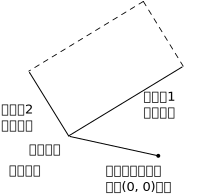
\includegraphics[width=51mm]{fig/chap2/Fig2.15a.pdf}
\begin{quote}
\heading{図2.15:} 枠は、原点と二つの辺という三つのベクトルによって記述される。
\end{quote}
\end{figure}

画像は、単位正方形内の座標\( (0 \le x, y \le 1) \)を使って記述することにします。
それぞれの枠には\jnewterm{枠座標マップ}(\newterm{frame coordinate map})
というものを関連づけ、画像が枠に合うようにずらしたり拡大縮小したりするのに
使います。このマップは、ベクトル\( {\bf v} = (x, y) \)を次のようなベクトルの和に
マップすることによって単位正方形を枠内に変換します。
\begin{comment}

\begin{example}
Origin(Frame) + x * Edge_1(Frame) + y * Edge_2(Frame)
\end{example}

\end{comment}
\begin{displaymath}
 {\rm Origin(Frame)} + x \cdot {\rm Edge_1(Frame)} + y \cdot {\rm Edge_2(Frame)}. 
\end{displaymath}
例えば、(0, 0)は枠の原点に、(1, 1)は原点と対角線上にある頂点に、
(0.5, 0.5)は枠の中心にマップされます。枠座標マップは次の手続きによって
作ることができます。
\footnote{\code{frame\-/coord\-/map}は、後で\link{練習問題 2.46}で記述する
ベクトル演算を使っています。これらは何らかのベクトルの表現を使って
実装されているとします。データ抽象化のおかげで、このベクトル表現がどのようなもので
あるかは、ふるまいさえ正しければ問題になりません。}

\begin{scheme}
(define (frame-coord-map frame)
  (lambda (v)
    (add-vect
     (origin-frame frame)
     (add-vect (scale-vect (xcor-vect v) (edge1-frame frame))
               (scale-vect (ycor-vect v) (edge2-frame frame))))))
\end{scheme}

\noindent
\code{frame\-/coord\-/map}をある枠に適用すると、ベクトルが与えられるとベクトルを
返す手続きを返します。引数ベクトルが単位正方形内にあれば、返り値のベクトルは
枠内のものになります。例えば、次の式は

\begin{scheme}
((frame-coord-map a-frame) (make-vect 0 0))
\end{scheme}

\noindent
以下と同じベクトルを返します。

\begin{scheme}
(origin-frame a-frame)
\end{scheme}

\begin{quote}
\heading{\phantomsection\label{練習問題 2.46}練習問題 2.46:} 
原点からある一点に張られる二次元ベクトルは、\( x \)座標と\( y \)座標からなる
ペアとして表現できる。コンストラクタ\code{make\-/vect}と、それに対応する
セレクタ\code{xcor\-/vect}, \code{ycor\-/vect}を与え、ベクトルに対する
データ抽象化を実装せよ。それらのセレクタとコンストラクタによって、ベクトルの
足し算、引き算、スカラによるかけ算という演算を行う手続き
\code{add\-/vect}, \code{sub\-/vect}, \code{scale\-/vect}を実装せよ。
\begin{comment}

\begin{example}
(x_1, y_1) + (x_2, y_2) = (x_1 + x_2, y_1 + y_2)
(x_1, y_1) - (x_2, y_2) = (x_1 - x_2, y_1 - y_2)
             s * (x, y) = (sx, sy)
\end{example}

\end{comment}
\begin{displaymath}
%
% \eqalign{
% 	(x_1, y_1) + (x_2, y_2) 	&= (x_1 + x_2, y_1 + y_2), \cr
% 	(x_1, y_1) - (x_2, y_2) 	&= (x_1 - x_2, y_1 - y_2), \cr
% 	s \cdot (x, y) 			&= (sx, sy). \cr }
% 
\begin{array}{r@{{}={}}l}
	(x_1, y_1) + (x_2, y_2) 	& (x_1 + x_2, y_1 + y_2), \\
	(x_1, y_1) - (x_2, y_2) 	& (x_1 - x_2, y_1 - y_2), \\
	s \cdot (x, y) 			& (sx, sy).
\end{array}
\end{displaymath}
\end{quote}

\begin{quote}
\heading{\phantomsection\label{練習問題 2.47}練習問題 2.47:} 
次に、枠のコンストラクタとして使えるものを二つ挙げる。

\begin{scheme}
(define (make-frame origin edge1 edge2)
  (list origin edge1 edge2))
(define (make-frame origin edge1 edge2)
  (cons origin (cons edge1 edge2)))
\end{scheme}

それぞれのコンストラクタに対し、適切なセレクタを加えて枠の実装を
完成させよ。
\end{quote}

\subsubsection*{ペインタ}

ペインタは、枠を引数として取り、ある特定の画像をずらしたり拡大縮小したりして
枠にフィットするように描画する手続きとして表現できます。つまり、\code{p}がペインタで
\code{f}がフレームであれば、\code{f}を引数として\code{p}を呼び出すことで、
\code{f}の中に\code{p}の画像を生成します。

基本ペインタがどのように実装されるかという具体的なところは、グラフィックシステムの
特性と描画する画像のタイプに依存します。例えば、二つの指定された点の間に
スクリーン上の線を引く\code{draw\-/line}という手続きを持っているとします。
すると、\link{図2.10}の\code{wave}ペインタのような線画のペインタは、
次のような線分のリストから作ることができます。
\footnote{
\code{segments\-/>painter}は、後で\link{練習問題 2.48}で記述する線分の表現を
使っています。また、\link{練習問題 2.23}で記述した\code{for\-/each}手続きも
利用しています。}

\begin{scheme}
(define (segments->painter segment-list)
  (lambda (frame)
    (for-each
     (lambda (segment)
       (draw-line
        ((frame-coord-map frame)
         (start-segment segment))
        ((frame-coord-map frame)
         (end-segment segment))))
     segment-list)))
\end{scheme}

\noindent
線分は、単位正方形に対する座標を使って与えられます。リスト中のそれぞれの線分に対し、
ペインタは線分の両端点を枠座標マップを使って変換し、変換した点の間に線を引きます。

ペインタを手続きとして表現することは、図形言語の中に強力な抽象化の壁を作ります。
さまざまなグラフィック機能に基づくいろいろな基本ペインタを作り、また組み合わせる
ことができます。枠を引数として取り、その枠に合わせて何かを描くものであれば、
どんな手続きでもペインタとして使うことができます。

\footnote{
例えば、\link{図2.11}の\code{rogers}ペインタはグレースケール画像によって
構築されています。枠内の各点に対し、\code{rogers}ペインタは枠座標マップによって
そこにマップされる画像内の点を決定し、それに従って点の濃淡をつけます。
\link{2.1.3節}では、有理数の実装はある適切な条件を満たすものであれば
何でもいいということを述べましたが、ここでさまざまな種類のペインタを使える
ようにしているのは、そこで述べた抽象データという考え方を利用したものです。
ここでは、指定された枠の中に何かを描画するものであれば、ペインタはどのような
実装でもいいということを利用しています。\link{2.1.3節}では
ペアを手続きとして実装する方法を示しましたが、ペインタはデータを手続きによって
表現する二つ目の例となっています。}

\begin{quote}
\heading{\phantomsection\label{練習問題 2.48}練習問題 2.48:} 
平面上の方向つきの線分は、ベクトルのペア---原点から線分の始点へと張られるベクトルと、
原点から線分の終点へと張られるベクトル---として表現できる。\link{練習問題 2.46}で
書いたベクトル表現を使って、\code{make\-/segment}というコンストラクタと
\code{start\-/segment}と\code{end\-/segment}というセレクタによって線分の
表現を定義せよ。
\end{quote}

\begin{quote}
\heading{\phantomsection\label{練習問題 2.49}練習問題 2.49:} 
\code{segments\-/>painter}を使って、以下の基本ペインタを定義せよ。

\begin{enumerate}[a.]

\item
指定された枠の輪郭を描くペインタ。

\item
枠の対角線同士をつないで``X''を描くペインタ。

\item
枠の辺の中点をつないで菱形を描くペインタ。

\item
\code{wave}ペインタ。

\end{enumerate}
\end{quote}

\subsubsection*{ペインタの変形と組み合わせ}

ペインタに対する演算(\code{flip\-/vert}や\code{beside}のようなもの)は、引数として
取った枠から導出した枠に対して元のペインタを呼び出すようなペインタを作るという
仕組みで動いています。ですので、例えば\code{flip\-/vert}が画像をひっくり返す際に、
ペインタがどのように動作しているかを知る必要はありません---枠をひっくり返す方法さえ
わかっていれば大丈夫です。ひっくり返したペインタは元のペインタをそのまま使いますが、
それをひっくり返した枠に対して使うというだけです。

ペインタ操作は、\code{transform\-/painter}という手続きに基づいています。
この手続きは引数として、ペインタと、枠をどのように変形するかという情報を取り、
新しいペインタを作ります。変形したペインタは、ある枠に対して呼ばれたとき、
その枠を変形して、変形した枠に対して元のペインタを呼び出します。
\code{transform\-/painter}の引数は(ベクトルとして表現した)複数の点で、
新しい枠の頂点を指定するものです。これらが枠に対してマップされるとき、
一つ目の点は新しい枠の原点を指定し、残り二つの点は枠の辺ベクトルの終点を
指定します。つまり、単位正方形内の引数は、元の枠内に含まれる枠を指定することに
なります。

\begin{scheme}
(define (transform-painter painter origin corner1 corner2)
  (lambda (frame)
    (let ((m (frame-coord-map frame)))
      (let ((new-origin (m origin)))
        (painter (make-frame
                  new-origin
                  (sub-vect (m corner1) new-origin)
                  (sub-vect (m corner2) new-origin)))))))
\end{scheme}

\noindent
ペインタの画像を上下逆にするには次のようにします。

\begin{scheme}
(define (flip-vert painter)
  (transform-painter painter
                     (make-vect 0.0 1.0)   ~\textrm{; new \code{origin}}~
                     (make-vect 1.0 1.0)   ~\textrm{; new end of \code{edge1}}~
                     (make-vect 0.0 0.0))) ~\textrm{; new end of \code{edge2}}~
\end{scheme}

\noindent
\code{transform\-/painter}を用いることで簡単に新しい変換を定義できます。
右上4分の1のフレームは次のようにして与えられます。

\begin{scheme}
(define (shrink-to-upper-right painter)
  (transform-painter
   painter (make-vect 0.5 0.5)
   (make-vect 1.0 0.5) (make-vect 0.5 1.0)))
\end{scheme}

\noindent
画像を反時計回りに90度回転させるという変形もあります。
\footnote{\code{rotate90}は回転した枠にフィットするように画像を伸縮させるという
ことも行うため、純粋な回転になるのは枠が正方形のときだけです。}

\begin{scheme}
(define (rotate90 painter)
  (transform-painter painter
                     (make-vect 1.0 0.0)
                     (make-vect 1.0 1.0)
                     (make-vect 0.0 0.0)))
\end{scheme}

\noindent
また、画像を枠の中心方向につぶすという変形もあります。
\footnote{\link{図2.10}と\link{図2.11}に出てきた菱形の画像は、
\code{squash\-/inwards}を\code{wave}と\code{rogers}に適用して作ったものです。}

\begin{scheme}
(define (squash-inwards painter)
  (transform-painter painter
                     (make-vect 0.0 0.0)
                     (make-vect 0.65 0.35)
                     (make-vect 0.35 0.65)))
\end{scheme}

\noindent
枠の変換は、二つ以上のペインタを組み合わせる手段を定義するためにキーとなるもの
でもあります。例えば、\code{beside}手続きは二つのペインタを引数に取り、
それらを引数の枠の左半分と右半分を描画するように変形し、新しい複合ペインタを
作ります。ある枠を引数として複合ペインタを呼び出すと、一つ目の変形ペインタを
呼んで枠の左半分を描画し、二つ目の変形ペインタを呼んで枠の右半分を描画します。

\begin{scheme}
(define (beside painter1 painter2)
  (let ((split-point (make-vect 0.5 0.0)))
    (let ((paint-left
           (transform-painter
            painter1
            (make-vect 0.0 0.0)
            split-point
            (make-vect 0.0 1.0)))
          (paint-right
           (transform-painter
            painter2
            split-point
            (make-vect 1.0 0.0)
            (make-vect 0.5 1.0))))
      (lambda (frame)
        (paint-left frame)
        (paint-right frame)))))
\end{scheme}

\noindent
ペインタのデータ抽象化と、特にペインタを手続きとして実装したことによって、
\code{beside}が実装しやすくなっているということがわかるでしょうか。
部品となるペインタについて\code{beside}が知っておくべきことは、それぞれの
ペインタが指定した枠に何かを描画するということだけで、そのほかには何も
知る必要がありません。

\begin{quote}
\heading{\phantomsection\label{練習問題 2.50}練習問題 2.50:} 
ペインタを左右逆にする変換\code{flip\-/horiz}、ペインタを反時計回りに
180度、270度回転させる変換を定義せよ。
\end{quote}

\begin{quote}
\heading{\phantomsection\label{練習問題 2.51}練習問題 2.51:} 
ペインタに対する\code{below}演算を定義せよ。\code{below}は二つのペインタを引数に取る。
返り値となるペインタは、枠が与えられたとき、一つ目のペインタで枠の下部を描画し、
二つ目のペインタで上部を描画する。二つのやり方で\code{below}を定義せよ。
一つ目は、上に示した\code{beside}手続きと似たような手続きを書くというもので、
二つ目は、\code{beside}と適切な回転演算(\link{練習問題 2.50}のもの)によって
定義するというものである。
\end{quote}

\subsubsection*{頑健な設計のための言語レベル}

図形言語は、手続きとデータによる抽象化についてこれまで紹介してきた重要な考え方の
練習となっています。基本的なデータ抽象化であるペインタは手続きによる表現を使って
実装され、異なる基礎的な描画機能を言語が統一したやり方で扱うことができるように
しています。結合手段は閉包性を満たしているため、複雑な設計も簡単に組み立てることが
できます。これで、手続きを抽象化するためのツールがすべて、ペインタの結合手段を
抽象化するのに利用できるということになります。

また、言語とプログラム設計についての、もうひとつの決定的な考え方を垣間見ることが
できました。それは\jnewterm{階層化設計}(\newterm{stratified design})というアプローチで、
複雑なシステムは一連の言語によって記述される一連のレベルとして構造化されるべきだという
概念です。それぞれのレベルは、そのレベルで基本とされる部品を組み合わせて構築され、
それぞれのレベルで構築された部品は次のレベルで基本部品として使われます。階層化設計の
それぞれのレベルで使われる言語は、その詳細さのレベルに合った基本要素、結合手段、
抽象化の手段を備えています。

階層化設計は、複雑なシステムのエンジニアリングのあらゆるところに出てきます。
例えば計算機工学では、抵抗やトランジスタを組み合わせて(またアナログ回路の言語を
使って記述して)ANDゲートやORゲートのような部品を作り、それらはデジタル回路設計の
言語では基本要素となります。\footnote{\link{3.3.4節}でそのような言語のひとつを
記述します。} これらの部品を組み合わせてプロセッサ、バス構造、メモリシステムを構築し、
今度はコンピュータアーキテクチャに適した言語を使ってそれらを組み合わせて
コンピュータを作ります。コンピュータは、ネットワーク相互接続を記述するのに適した
言語を使って組み合わされて分散システムを構成します。こういった繰り返しです。

階層化のごく小さな例として、ここでの図形言語は基本要素(基本ペインタ)を使っていますが、
それらの基本要素は、\code{segments\-/>painter}の線分のリストや\code{rogers}のような
ペインタの濃淡の詳細点や線を規定する言語を使って作られたものです。図形言語についての
説明の大半は、これらの基本要素を組み合わせることや、\code{beside}や\code{below}の
ような幾何学的な結合器に焦点を当てていました。さらに、\code{beside}や
\code{below}を言語の基本要素と見なすことで、さらに高いレベルでの作業も行いました。
その言語の\code{square\-/of\-/four}のような演算は、幾何学的な結合器を組み合わせる
際のよくあるパターンを捉えています。

階層化設計は、\jnewterm{頑健}(\newterm{robust})なプログラムを作りやすくします。
頑健というのは、仕様の小さな変更が、プログラム上でも相応に小さな変更ですむという
ことです。例えば、\link{図2.9}に示した、\code{wave}をもとにした画像を変更
したいとします。このとき、最も下のレベルに手を加え、\code{wave}の細かい見た目を
変えることもできます。また、中間レベルで、\code{corner\-/split}が
\code{wave}を複製するやり方を変えることもできます。最も上のレベルで、
\code{square\-/limit}が四隅の画像を配置するやり方を変えることもできます。
一般的に、階層化設計のそれぞれのレベルは、システムの特性を表現するうえでの
異なる語彙を提供し、システムを変更するための異なる能力を提供します。

\begin{quote}
\heading{\phantomsection\label{練習問題 2.52}練習問題 2.52:} 
上で述べた各レベルに手を加え、\link{図2.9}に示した\code{wave}による
square-limitを変更せよ。具体的には、次のようなものである。

\begin{enumerate}[a.]

\item
\link{練習問題 2.49}の\code{wave}基本ペインタに線分をいくつか加えよ
(例えば、笑顔を追加するなど)。

\item
\code{corner\-/split}によって構築されるパターンを変更せよ
(例えば、\code{up\-/split}や\code{right\-/split}の画像を二つではなく一つだけ使う
ようにする)。

\item
\code{square\-/of\-/four}を使うほうの\code{square\-/limit}を修正し、
四隅を違うパターンで組み立てるようにせよ(例えば、正方形の四隅で大きなロジャーズ氏が
外を向くようにするなど)。

\end{enumerate}
\end{quote}

\section{記号データ}
\label{2.3節}

ここまで使ってきた複合データオブジェクトはすべて、究極的には数値から構成されて
いました。この節では、任意の記号をデータとして扱う能力を導入し、私たちの言語の
表現能力を拡張します。

\subsection{クォート}
\label{2.3.1節}

記号を作って複合データを作れるとしたら、次のようなリストが使えることになります。

\begin{scheme}
(a b c d)
(23 45 17)
((Norah 12) (Molly 9) (Anna 7) (Lauren 6) (Charlotte 4))
\end{scheme}

\noindent
記号を含むリストは、私たちの言語の次のような式と同じように見えるかもしれません。

\begin{scheme}
(* (+ 23 45)
   (+ x 9))
(define (fact n)
  (if (= n 1) 1 (* n (fact (- n 1)))))
\end{scheme}

\noindent
記号を操作するためには、私たちの言語に新しい要素を入れる必要があります。
それは、データオブジェクトを\jnewterm{クォート}(\newterm{quote})する能力です。
\code{(a b)}というリストを構築するという場合について考えてみましょう。
これは、\code{(list a b)}と書いてもうまくいきません。この式は、\code{a}や\code{b}と
いった記号そのものではなく、その\jnewterm{値}(\newterm{value})を要素としたリストを
作ってしまうからです。この問題は、自然言語についてはよく知られています。自然言語では、
単語や文が意味的な実体となることもあり、文字の列(統語的な実体)となることもあります。
自然言語では、単語や文をそのまま文字の列として扱うということを示すのに、
引用符を使うのが一般的です。例えば、``John''の最初の文字というと、それは当然``J''
です。誰かに``あなたの名前を声に出して言ってください''と頼んだら、その人の名前を
言ってくれるでしょう。しかし、`` `あなたの名前'を声に出して言ってください''と
頼んだら、``あなたの名前''という単語列を言ってもらえるはずです。ほかの人の
発言を伝えるために、引用符をネストさせないといけなくなっていることに気をつけて
ください。
\footnote{言語でクォートを使えるようにすると、等しいものは等しいもので
置き換えられるという概念を破壊するため、言語を単純に推論する能力を台無しに
してしまいます。例えば、三は一足す二ですが、「三」という単語は「一足す二」という
句ではありません。クォートを使うと、ほかの式を操作する式を作れるようになるので、
そういう意味でクォートは強力です(これについては、\link{第4章}でインタプリタを
書く際に見ることになります)。しかし、ある言語の中で、その言語で書かれた文について
表現する文というものを許すと、「等しいもの同士は交換できる」ということが
何を意味するのかについて、一貫性のある原則を維持することがとても難しくなります。
例えば、もし宵の明星は明けの明星であると知っていれば、「宵の明星は金星である」
という文から、「明けの明星は金星である」と推論できます。しかし、「ジョンは
宵の明星は金星であると知っている」ということからは、「ジョンは明けの明星は
金星であると知っている」を導くことはできません。}

リストや記号について、式として評価の対象にするのでなく、データオブジェクトとして
扱いたいというときにも、これと同じような慣例に従うことができます。しかし、
ここでのクォートの形式は、自然言語の場合と違って、クォートするオブジェクトの前に
引用符(伝統的にシングルクォートの記号 \code{'}を使います)をひとつだけ置く
というものです。Schemeの文法では、オブジェクトを区切るのに空白や括弧を使っているため、
クォートはひとつだけで問題ありません。このようなわけで、シングルクォートは
次のオブジェクトをクォートするという意味になっています。
\footnote{表示する文字列を囲むのにはダブルクォートを使ってきましたが、シングル
クォートはそれとは違うものです。シングルクォートはリストや記号を表すのに使われる
のに対して、ダブルクォートは文字列にしか使われません。この本では、文字列を使うのは
項目を表示する場合だけです。}

これで、記号とその値を区別できるようになりました。

\begin{scheme}
(define a 1)
(define b 2)
(list a b)
~\textit{(1 2)}~
(list 'a 'b)
~\textit{(a b)}~
(list 'a b)
~\textit{(a 2)}~
\end{scheme}

\noindent
リストを表示するときに使う慣習的な表現を使って複合オブジェクトを入力することも、
クォートによってできるようになります。
\footnote{厳密に言うと、この引用符の使い方は、言語内のすべての複合式は括弧で
囲まれていてリストのように見えるという一般的な規則を破っています。ここで、
\code{quote}という特殊形式を導入することによって、この一貫性を取り戻すことができます。
\code{quote}の役割はクォートと同じです。つまり、\code{'a}の代わりに\code{(quote a)}と
入力したり、\code{'(a b c)}の代わりに\code{(quote (a b c))}と入力したり
できます。これはインタプリタの動作方式そのままです。引用符は、次に来る完全な式を
\code{quote}を使って包んで、\( \hbox{\ttfamily(quote}\;\langle\kern0.06em
\hbox{\ttfamily\slshape expression}\kern0.08em\rangle\hbox{\ttfamily)} \)を
作るということを、一文字に省略したものにすぎません。これは重要なポイントです。
こうすることによって、インタプリタから見える式はすべてデータオブジェクトとして
操作できるという原則を維持できるからです。例えば、\code{(car '(a b c))}という
式は\code{(car (quote (a b c)))}と同じものなので、
\code{(list 'car (list 'quote '(a b c)))}を評価することによって構築できます。}

\begin{scheme}
(car '(a b c))
~\textit{a}~
(cdr '(a b c))
~\textit{(b c)}~
\end{scheme}

\noindent
この原則通りに、\code{'()}を評価すると空リストが得られます。これによって、
変数\code{nil}は必要なくなります。

記号の操作に使われるもうひとつの基本要素は\code{eq?}です。これは二つの記号を
引数として取り、それらが同じであるかどうかをテストするものです。
\footnote{
二つの記号が同じ順番の同じ文字で構成されているとき、それらは``同じ''であると
考えることができます。このような定義は、まだここでは取り組むことが難しい、
プログラミング言語における``同一性''の意味とは何かという深い問題を
避けて通っています。\link{第3章} (\link{3.1.3節})では、この問題に
戻ってくることになります。}
\code{eq?}を使うと、\code{memq}という便利な手続きを実装できます。
これは記号とリストという二つの引数を取り、記号がリストに含まれていなければ
(つまり、リストのどの項目とも\code{eq?}でなければ)、\code{memq}は偽を返します。
そうでなければ、そのリストの中で記号が最初に見つかったところから始まる
サブリストを返します。

\begin{scheme}
(define (memq item x)
  (cond ((null? x) false)
        ((eq? item (car x)) x)
        (else (memq item (cdr x)))))
\end{scheme}

\noindent
例えば、次の式の値は偽になります。

\begin{scheme}
(memq 'apple '(pear banana prune))
\end{scheme}

\noindent
一方、次の式の値は\code{(apple pear)}になります。

\begin{scheme}
(memq 'apple '(x (apple sauce) y apple pear))
\end{scheme}

\noindent

\begin{quote}
\heading{\phantomsection\label{練習問題 2.53}練習問題 2.53:} 
以下の式をそれぞれ評価したとき、それらに対してインタプリタは何を表示するか。

\begin{scheme}
(list 'a 'b 'c)
(list (list 'george))
(cdr '((x1 x2) (y1 y2)))
(cadr '((x1 x2) (y1 y2)))
(pair? (car '(a short list)))
(memq 'red '((red shoes) (blue socks)))
(memq 'red '(red shoes blue socks))
\end{scheme}
\end{quote}

\begin{quote}
\heading{\phantomsection\label{練習問題 2.54}練習問題 2.54:} 
二つのリストは、同じ要素を同じ順番で持つときに\code{equal?}であると言える。
例えば、

\begin{scheme}
(equal? '(this is a list) '(this is a list))
\end{scheme}

\noindent
は真である。しかし、

\begin{scheme}
(equal? '(this is a list) '(this (is a) list))
\end{scheme}

\noindent
は偽である。より正確に言うと、記号が等しいかどうかという基本的な\code{eq?}を使って、
再帰的に\code{equal?}を定義できる。\code{a}と\code{b}は、どちらも記号で
あってそれらが\code{eq?}であるか、どちらもリストであって、\code{(car a)}と\code{(car b)}が
\code{equal?}であり、かつ\code{(cdr a)}と\code{(cdr b)}が\code{equal?}である場合、
\code{equal?}である。この考え方を使って、\code{equal?}を手続きとして実装せよ。
\footnote{実際は、プログラマは記号だけでなく数値も含むリストに対して\code{equal?}を使うことも
あります。数値は記号とは見なされません。数として等しい二つの数値(\code{=}でテストできます)が
\code{eq?}でもあるかという問題は、高度に実装依存です。\code{equal?}の定義としては、
(Schemeで基本要素となっているもののように)\code{a}と\code{b}が両方とも数値である場合、
\code{a}が\code{b}が数として等しければそれらは\code{equal?}であるということも
規定しておくほうがよいでしょう。}
 
\end{quote}

\begin{quote}
\heading{\phantomsection\label{練習問題 2.55}練習問題 2.55:} 
Eva Lu Atorはインタプリタに次の式を入力した。

\begin{scheme}
(car ''abracadabra)
\end{scheme}

予想外なことに、インタプリタは\code{quote}という表示を返してきた。このことを説明せよ。
\end{quote}


\subsection{例: 記号微分}
\label{2.3.2節}

記号操作の例として、またデータ抽象化の別の例として、代数式の記号微分を行う
手続きの設計について考えてみましょう。手続きは、引数として代数式と変数を取り、
その変数に関するその式の導関数を返すようにします。例えば、手続きに対する引数が
\( ax^2 + bx + c \)と\( x \)であれば、手続きは\( 2ax + b \)を返すというものです。
記号微分は、Lispにとっては特別な歴史的意義があります。記号微分は、記号を操作する
コンピュータ言語を開発するうえでの動機となる実例のひとつでした。さらに、記号微分の
研究は、現在応用数学者や物理学者に使われるようになってきている強力な記号数式処理
システムの開発につながる一連の研究のスタート地点となるものです。

記号微分プログラムを開発するにあたっては、\link{2.1.1節}の有理数システムを開発した
ときと同じデータ抽象化戦略に従います。つまり、まず``和''、``積''、``変数''といった
抽象オブジェクトの上で動く微分アルゴリズムを定義することにして、それらの抽象オブジェクトが
どのように表現されるべきかということは考えないことにします。表現の問題については
後ほど取り組みます。

\subsubsection*{抽象データによる微分プログラム}

問題を簡単にするために、二引数の足し算・かけ算という演算だけから構成される式だけを
扱う、とても単純な記号微分プログラムについて考えることにします。任意のそのような式の
微分は、以下の簡約規則を適用することによって行うことができます。
\begin{comment}

\begin{example}
dc
-- = 0  for c a constant, or a variable different from x
dx

dx
-- = 1
dx

d(u + v)   du   dv
-------- = -- + --
   dx      dx   dx

d(uv)     / dv \     / du \
----- = u | -- | + v | -- |
 dx       \ dx /     \ dx /
\end{example}

\end{comment}
\begin{displaymath}
{{\it dc} \over {\it dx}} 		= 0,
	\quad c\ \mbox{が定数または} x\ \mbox{と異なる変数のとき},
\end{displaymath}
\begin{displaymath}
{{\it dx} \over {\it dx}} 		= 1,
\end{displaymath}
\begin{displaymath}
{{\it d\,(u + v\,)} \over {\it dx}} 	= {{\it du} \over {\it dx}} + {{\it dv} \over {\it dx}},
\end{displaymath}
\begin{displaymath}
{{\it d\,(uv\,)} \over {\it dx}} 	= u {{\it dv} \over {\it dx}} + v {{\it du} \over {\it dx}}.
\end{displaymath}

\noindent
後ろの二つの規則は本質的に再帰的であるということがわかるでしょうか。
というのは、和の導関数を求める際には、まずそれぞれの項の導関数を求め、それらを
足すことになるからです。それぞれの項は、さらに分解が必要な式であるかもしれません。
項をどんどん小さなものに分解していくと、最終的には定数か変数のものになり、
その導関数は0または1になります。

これらの規則を手続きという形にするために、有理数の実装を設計したときと同じように、
ちょっとした希望的思考をすることにします。もし代数式の表現手段があるとするなら、
ある式が和なのか、積なのか、定数なのか、変数なのか識別できるはずです。また、
式から構成要素を抽出することもできるでしょう。和については、例えば加数(第一項)と
被加数(第二項)を抽出できるようになっていてほしいところです。それに、構成要素から
式を構築することもできるはずです。ここでは、次のようなセレクタ、コンストラクタ、
述語を実装する手続きがもうできているとします。

\begin{scheme}
(variable? e)            ~\textrm{\code{e}は変数か?}~
(same-variable? v1 v2)   ~\textrm{\code{v1}と\code{v2}は同じ変数か?}~
(sum? e)                 ~\textrm{\code{e}は和か?}~
(addend e)               ~\textrm{和\code{e}の加数}~
(augend e)               ~\textrm{和\code{e}の被加数}~
(make-sum a1 a2)         ~\textrm{\code{a1}と\code{a2}の和を構築する}~
(product? e)             ~\textrm{\code{e}は積か?}~
(multiplier e)           ~\textrm{積\code{e}の乗数}~
(multiplicand e)         ~\textrm{積\code{e}の被乗数}~
(make-product m1 m2)     ~\textrm{\code{m1}と\code{m2}の積を構築する}~
\end{scheme}

\noindent
これらの手続きと、数値かどうかを判断する基本述語の\code{number?}を使って、
微分の規則を次の手続きのように表現できます。

\begin{scheme}
(define (deriv exp var)
  (cond ((number? exp) 0)
        ((variable? exp) (if (same-variable? exp var) 1 0))
        ((sum? exp) (make-sum (deriv (addend exp) var)
                              (deriv (augend exp) var)))
        ((product? exp)
         (make-sum
           (make-product (multiplier exp)
                         (deriv (multiplicand exp) var))
           (make-product (deriv (multiplier exp) var)
                         (multiplicand exp))))
        (else
         (error "unknown expression type: DERIV" exp))))
\end{scheme}

\noindent
この\code{deriv}手続きには、完全な微分アルゴリズムが組み込まれています。
抽象データによって表現されているため、ちゃんとしたセレクタとコンストラクタの
セットを設計する限り、代数式をどう表現したとしても動くはずです。この問題については
次で見ていきます。

\subsubsection*{代数式を表現する}

リスト構造を使って代数式を表現するやり方はいろいろ考えられます。例えば、
通常の代数記法を反映した記号のリストを使って、\( ax + b \)を\code{(a * x + b)}
というリストとして表現するということも可能です。ですが、とりわけ素直なやり方は、
Lisp が複合式に使うのと同じ、括弧でくくった前置記法を使うというものです。
つまり、\( ax + b \)は\code{(+ (* a x) b)}と表現することになります。そうすると、
微分問題に対するデータ表現は次のようになります。

\begin{itemize}

\item
変数は記号である。基本述語\code{symbol?}で識別する。

\begin{scheme}
(define (variable? x) (symbol? x))
\end{scheme}

\item
二つの変数は、それらを表現する記号が\code{eq?}であれば等しい。

\begin{scheme}
(define (same-variable? v1 v2)
  (and (variable? v1) (variable? v2) (eq? v1 v2)))
\end{scheme}

\item
和と積は、リストとして構築する。

\begin{scheme}
(define (make-sum a1 a2) (list '+ a1 a2))
(define (make-product m1 m2) (list '* m1 m2))
\end{scheme}

\item
和は、最初の要素が記号\code{+}であるリストである。

\begin{scheme}
(define (sum? x) (and (pair? x) (eq? (car x) '+)))
\end{scheme}

\item
加数は、和のリストの二つ目の項である。

\begin{scheme}
(define (addend s) (cadr s))
\end{scheme}

\item
被加数は、和のリストの三つ目の項である。

\begin{scheme}
(define (augend s) (caddr s))
\end{scheme}

\item
積は、最初の要素が記号\code{*}であるリストである。

\begin{scheme}
(define (product? x) (and (pair? x) (eq? (car x) '*)))
\end{scheme}

\item
乗数は、積のリストの二つ目の項である。

\begin{scheme}
(define (multiplier p) (cadr p))
\end{scheme}

\item
被乗数は、積のリストの三つ目の項である。

\begin{scheme}
(define (multiplicand p) (caddr p))
\end{scheme}

\end{itemize}

\noindent
こうすると、\code{deriv}に具体的に書いたようなアルゴリズムによってこれらの要素を
組み合わせるだけで、ちゃんと動く記号微分プログラムができます。そのふるまいについて、
いくつかの例を見てみましょう。

\begin{scheme}
(deriv '(+ x 3) 'x)
~\textit{(+ 1 0)}~
(deriv '(* x y) 'x)
~\textit{(+ (* x 0) (* 1 y))}~
(deriv '(* (* x y) (+ x 3)) 'x)
~\textit{(+ (* (* x y) (+ 1 0))}~
   ~\textit{(* (+ (* x 0) (* 1 y))}~
      ~\textit{(+  x 3)))}~
\end{scheme}

\noindent
プログラムは正しい答えを返します。しかし、答えは簡約されていません。次の結果は、確かに
正しいものです。
\begin{comment}

\begin{example}
d(xy)
----- = x * 0 + 1 * y
 dx
\end{example}

\end{comment}
\begin{displaymath}
 {{\it d\,(xy\,)} \over {\it dx}} = x \cdot 0 + 1 \cdot y
\end{displaymath}
しかし、プログラムには\( x \cdot 0 = 0 \), \( 1 \cdot y = y \), \( 0 + y = y \)だという
ことをわかっていてほしいものです。二つ目の例の答えは、単純に\code{y}であるべきです。
三つ目の例でわかるように、式が複雑であるとこれは深刻な問題になってきます。

ここで問題になっていることは、有理数の実装の際に問題になったこととよく似ています。
答えが最も単純な形に簡約されていないという問題です。有理数の簡約は、実装の中で
コンストラクタとセレクタだけを変更するだけでできました。ここでも、同じような戦略が
使えます。\code{deriv}にはまったく手を加えないことにします。その代わり、
\code{make\-/sum}に変更を加え、もし両方の加数が数値であれば、それらを足し合わせて
和を返すようにします。また、加数のひとつが0であれば、もうひとつの加数のみを返すように
します。

\begin{scheme}
(define (make-sum a1 a2)
  (cond ((=number? a1 0) a2)
        ((=number? a2 0) a1)
        ((and (number? a1) (number? a2))
         (+ a1 a2))
        (else (list '+ a1 a2))))
\end{scheme}

\noindent
ここでは、ある式が与えられた数値と等しいかどうかをチェックする\code{=number?}という
手続きを使っています。

\begin{scheme}
(define (=number? exp num) (and (number? exp) (= exp num)))
\end{scheme}

\noindent
同じように、\code{make\-/product}に変更を加えて、0には何をかけても0で、1に何かをかけると
その何か自身になるという規則を組み込みます。

\begin{scheme}
(define (make-product m1 m2)
  (cond ((or (=number? m1 0) (=number? m2 0)) 0)
        ((=number? m1 1) m2)
        ((=number? m2 1) m1)
        ((and (number? m1) (number? m2)) (* m1 m2))
        (else (list '* m1 m2))))
\end{scheme}

\noindent
今回のものが、先ほどの三つの例に対してどう動作するかを次に示します。

\begin{scheme}
(deriv '(+ x 3) 'x)
~\textit{1}~
(deriv '(* x y) 'x)
~\textit{y}~
(deriv '(* (* x y) (+ x 3)) 'x)
~\textit{(+ (* x y) (* y (+ x 3)))}~
\end{scheme}

\noindent
これでだいぶよくなりましたが、三つ目の例を見ると、式を誰もが``最も単純''だといえる
ような形にするプログラムができるまでには、まだだいぶ距離がありそうです。代数的簡約化の
問題は、何よりも、ある目的のためには最も単純である形式がほかの目的のためには
そうではないということがありうるため、複雑なものになっています。

\begin{quote}
\heading{\phantomsection\label{練習問題 2.56}練習問題 2.56:} 
より多くの種類の式を扱えるようにこの基本的な微分プログラムを拡張するには
どうすればよいかを示せ。例えば、次の微分規則を実装せよ。
\begin{comment}

\begin{example}
d(u^n)            du
------ = nu^(n-1) --
  dx              dx
\end{example}

\end{comment}
\begin{displaymath}
 {{\it d\,(u^n\,)} \over {\it dx}} = nu^{n-1} {{\it du} \over {\it dx}} 
\end{displaymath}
実装にあたっては、\code{deriv}プログラムに新しい節を追加し、また
\code{exponentiation?}, \code{base}, \code{exponent}, \code{make\-/exponentiation}を
適切に定義せよ(冪乗の表現には\code{**}という記号を使ってもよい)。任意の数の0乗は
1であり、任意の数の1乗はそれ自身であるという規則を組み込め。
\end{quote}

\begin{quote}
\heading{\phantomsection\label{練習問題 2.57}練習問題 2.57:} 
微分プログラムを拡張し、(2以上の)任意の数の項の和と積を扱えるようにせよ。
すると上の最後の例は以下のように表現できる。

\begin{scheme}
(deriv '(* x y (+ x 3)) 'x)
\end{scheme}

\code{deriv}手続きにはまったく手を加えず、和と積の表現のみを変更することによって解け。
例えば、和の\code{addend}(加数)は最初の項で、\code{augend}(被加数)は残りの項の和と
いうようにする。
\end{quote}

\begin{quote}
\heading{\phantomsection\label{練習問題 2.58}練習問題 2.58:} 
微分プログラムを修正して、\code{+}と\code{*}が前置演算子ではなく中置演算子となるような、
通常の数学の記法に対して動作させたいとする。微分プログラムは抽象データによって定義されて
いるので、微分プログラムの動作基盤となる代数式の表現を定義する述語、セレクタ、コンストラクタを
変更するだけで、異なる表現を扱うように修正できる。

\begin{enumerate}[a.]

\item
\code{(x + (3 * (x + (y + 2))))}のような中置記法で表された代数式を微分するには
どのようにするかを示せ。問題を簡単にするため、\code{+}と\code{*}は常に二つの
引数を取り、式は完全に括弧でくくられていると仮定せよ。

\item
\code{(x + 3 * (x + y + 2))}のような標準的な代数記法を認めると、問題はずっと
難しくなる。この記法では、必要のない括弧は省略し、乗算は加算より先に行われると
仮定している。ここでの微分プログラムがそのような記法に対してもうまく動くように、
適切な述語、セレクタ、コンストラクタを設計できるだろうか。

\end{enumerate}
\end{quote}

\subsection{例: 集合を表現する}
\label{2.3.3節}

ここまでの例では、有理数と代数式という、二種類の複合データオブジェクトの表現を
構築しました。この例のうちのひとつでは、式の単純化(簡約化)をコンストラクタで
行うかセレクタで行うかという選択肢がありましたが、そのほかの点では、これらの
構造のリストによる表現の選択肢は素直なものでした。しかし、集合の表現ということに
なると、表現をどう決めるかということはあまり明らかではありません。実際に、
可能な表現は数多くあり、それぞれいくつかの点でお互いに大きく異なっています。

ざっくりした言い方をすると、集合とはただの異なるオブジェクトの集まりです。より
正確な定義をするには、データ抽象化の手法を使うことができます。つまり、
集合に使われる演算を規定することによって``集合''を定義するということです。
それらの演算は、\code{union\-/set}, \code{intersection\-/set}, \code{element\-/of\-/set?},
\code{adjoin\-/set}です。
\code{element\-/of\-/set?}は、与えられた要素が集合の構成要素であるかどうかを判定する
述語です。\code{adjoin\-/set}は、オブジェクトと集合を引数に取り、元の集合の要素に加えて
追加された要素を含む集合を返します。\code{union\-/set}は、二つの集合の和集合、
つまりどちらかの引数に含まれる要素をすべて含む集合を計算します。\code{intersection\-/set}は、
二つの集合の共通部分、つまり引数のどちらにも含まれる要素のみを含む集合を計算します。
データ抽象という視点から見ると、上の解釈と整合性があるものでさえあれば、これらの演算を
実装するのにどのような表現でも自由に設計できます。
\footnote{
さらに形式的に書くなら、``上の解釈と整合性がある''というところを、演算が次のような
一連の規則を満たすというように規定できます。

\noindent
任意の集合\code{S}と任意のオブジェクト\code{x}に対し、
\code{(element\-/of\-/set? x (adjoin\-/set x S))}は真である(ざっくり言うと、
``集合にオブジェクトを追加すると、そのオブジェクトを含む集合ができる'')。

\noindent
任意の集合\code{S}, \code{T}と任意のオブジェクト\code{x}に対し、
\code{(element\-/of\-/set? x (union\-/set S T))}は
\code{(or (element\-/of\-/set? x S) (element\-/of\-/set? x T))}に等しい。
(ざっくり言うと、``\code{(union S T)}の要素は、\code{S}に含まれる要素か、
\code{T}に含まれる要素である'')。

\noindent
任意のオブジェクト\code{x}に対し、\code{(element\-/of\-/set? x '())}は偽である
(ざっくり言うと、``空集合の要素となるオブジェクトは存在しない'')。
}

\subsubsection*{順序なしリストとしての集合}

リストを表現するやり方のひとつは、要素が二回以上現れることがないリストという
ものです。空集合は空リストとして表現します。この表現では、\code{element\-/of\-/set?}は
\link{2.3.1節}の\code{memq}手続きと似たものになります。ここでは\code{eq?}ではなく
\code{equal?}を使っているため、集合の要素は記号である必要はありません。

\begin{scheme}
(define (element-of-set? x set)
  (cond ((null? set) false)
        ((equal? x (car set)) true)
        (else (element-of-set? x (cdr set)))))
\end{scheme}

\noindent
これを使って、\code{adjoin\-/set}を書くことができます。追加するオブジェクトがすでに
集合の中にあるなら、単にその集合を返します。そうでなければ、\code{cons}を使って
そのオブジェクトを集合を表すリストに追加します。

\begin{scheme}
(define (adjoin-set x set)
  (if (element-of-set? x set)
      set
      (cons x set)))
\end{scheme}

\noindent
\code{intersection\-/set}には、再帰的な戦略が使えます。もし、\code{set2}と、
\code{set1}の\code{cdr}との共通部分を作ることができるなら、\code{set1}の
\code{car}をそれに含めるかどうかを決めるだけで十分です。しかし、これは
\code{(car set1)}が\code{set2}にも含まれているかどうかによって決まります。
結果として、手続きは次のようになります。

\begin{scheme}
(define (intersection-set set1 set2)
  (cond ((or (null? set1) (null? set2)) '())
        ((element-of-set? (car set1) set2)
         (cons (car set1) (intersection-set (cdr set1) set2)))
        (else (intersection-set (cdr set1) set2))))
\end{scheme}

\noindent
表現を設計する際に考慮するべき問題のひとつは効率です。この集合演算に必要となる
ステップ数を考えてみましょう。どの演算も\code{element\-/of\-/set?}を使っているので、
この演算の速度は集合の実装全体の効率に大きな影響を与えます。ここで、あるオブジェクトが
集合の要素かどうかチェックするために、\code{element\-/of\-/set?}は集合全体を
走査する必要があるかもしれません(最悪の場合、オブジェクトは集合の中になかったという
結果になります)。そのため、集合が\( n \)個の要素を持っているとすると、
\code{element\-/of\-/set?}には最大\( n \)ステップかかるかもしれません。つまり、
必要なステップ数は\( \Theta(n) \)で増加するということです。\code{adjoin\-/set}は
この演算を使うので、やはり\( \Theta(n) \)で増加します。\code{intersection\-/set}は、
\code{set1}の要素それぞれに対して\code{element\-/of\-/set?}のチェックをするため、
必要なステップ数は関係する集合の大きさの積に比例して増加、つまり大きさ\( n \)の二つの集合
に対して\( \Theta(n^2) \)で増加するということになります。\code{union\-/set}についても
同じことが言えます。

\begin{quote}
\heading{\phantomsection\label{練習問題 2.59}練習問題 2.59:} 
順序なしリストとして表現した集合に対する\code{union\-/set}演算を実装せよ。
\end{quote}

\begin{quote}
\heading{\phantomsection\label{練習問題 2.60}練習問題 2.60:}
上の例では、集合は重複のないリストとして表現するよう規定した。ここで、重複を許す
場合について考えてみよう。その場合、例えば\( \{1, 2, 3\} \)という集合は
\code{(2 3 2 1 3 2 2)}というリストとして表現することもできる。この表現に対して
演算を行う手続き\code{element\-/of\-/set?}, \code{adjoin\-/set}, \code{union\-/set},
\code{intersection\-/set}を設計せよ。それぞれの効率は、重複なし表現に対する手続きで
それに対応するものと比べてどうだろうか。重複なしの表現よりもこの表現のほうが
向いているような応用はあるだろうか。
\end{quote}

\subsubsection*{順序つきリストとしての集合}

この集合演算を速くする方法のひとつとして、集合の要素が昇順に並ぶように
表現を変えるというものがあります。これをするためには、二つのオブジェクトを
比較してどちらが大きいか判断するための何らかの方法が必要です。例えば、
記号を辞書順に比較したり、オブジェクトに一意の数値を割り振ることに決めて
対応する数値によって要素を比較したりといったことが考えられます。ここでは
話を簡単にするため、集合の要素が数値である場合についてのみ考えることにします。
この場合、要素は\code{>}と\code{<}によって比較できます。数値の集合を表現するのには、
要素を昇順に並べたものを使います。上に挙げた最初の表現では、\( \{1, 3, 6, 10\} \)
という集合を表すのに要素をどのように並べてもかまいませんでしたが、
新しい表現では\code{(1 3 6 10)}というリストしか許可しません。

順序に従って並べることのひとつの利点は\code{element\-/of\-/set?}で出てきます。
項目があるかどうかを調べるのに、もう集合全体を走査する必要はありません。
探している項目よりも大きい要素に出会ったら、その項目が集合内にないということが
わかります。

\begin{scheme}
(define (element-of-set? x set)
  (cond ((null? set) false)
        ((= x (car set)) true)
        ((< x (car set)) false)
        (else (element-of-set? x (cdr set)))))
\end{scheme}

\noindent
これはどれだけのステップ数の節約になるでしょうか。最悪の場合、探している項目は
集合内の一番大きなものかもしれず、その場合ステップ数は順序なし表現の場合と
同じです。しかし、いろいろな大きさの項目を検索するときのことを考えると、
場合によってはリストの始点のあたりで検索を終了できたり、
場合によってはやっぱりリストのほとんどを調べないといけなかったり、となることが
期待できます。平均的には、集合の約半分の項目を検査しなければいけないということに
なるでしょう。このため、必要な平均ステップ数はだいたい\( n / 2 \)になります。
これは依然として\( \Theta(n) \)という増加オーダーですが、それでもやはり、平均的には、
前の実装に比べてステップ数を半分に節約できます。

\code{intersection\-/set}では、さらに目覚ましい高速化が達成できます。順序なし表現では、
この演算には\( \Theta(n^2) \)というステップ数が必要でした。それは、\code{set1}の
要素それぞれに対して\code{set2}の完全な走査を行っていたからでした。しかし、
順序つきの表現では、より賢い方法が使えます。まず、二つの集合の最初の要素
\code{x1}と\code{x2}を比較します。もし\code{x1}と\code{x2}が等しければ、それは
共通部分の要素になり、共通部分の残りは二つの集合の\code{cdr}の共通部分という
ことになります。では、\code{x1}が\code{x2}より小さい場合はどうなるか考えてみましょう。
\code{x2}は\code{set2}の最小要素なので、\code{x1}は\code{set2}のどこにも現れないと
結論づけることができます。つまり、共通部分にも含まれないということになります。
このため共通部分は、\code{set2}と、\code{set1}の\code{cdr}との共通部分に等しくなります。
同じように、もし\code{x2}が\code{x1}よりも小さければ、求める共通部分は、\code{set1}と、
\code{set2}の\code{cdr}との共通部分となります。手続きは次のようになります。

\begin{scheme}
(define (intersection-set set1 set2)
  (if (or (null? set1) (null? set2))
      '()
      (let ((x1 (car set1)) (x2 (car set2)))
        (cond ((= x1 x2)
               (cons x1 (intersection-set (cdr set1)
                                          (cdr set2))))
              ((< x1 x2)
               (intersection-set (cdr set1) set2))
              ((< x2 x1)
               (intersection-set set1 (cdr set2)))))))
\end{scheme}

\noindent
このプロセスで必要となるステップ数を見積もるには、各ステップで、共通部分問題を
より小さな集合の共通部分集合の計算に縮小していることに注意してください。
縮小は、\code{set1}と\code{set2}のどちらかまたは両方から最初の要素を削除することに
よって行われます。このため、必要なステップ数は、最大でも\code{set1}と\code{set2}の
大きさの合計で、順序なし表現のように大きさの積になることはありません。これは、
\( \Theta(n^2) \)というオーダーに対して\( \Theta(n) \)というオーダーになるという
ことで、そこそこの大きさの集合に対してもかなりの高速化になります。

\begin{quote}
\heading{\phantomsection\label{練習問題 2.61}練習問題 2.61:} 
順序つき表現を使った\code{adjoin\-/set}を実装せよ。\code{element\-/of\-/set?}から
類推して、順序つきであることの利点を生かして、順序なしの表現に比べて平均的に半分の
ステップを必要とする手続きを作るやり方を示せ。
\end{quote}

\begin{quote}
\heading{\phantomsection\label{練習問題 2.62}練習問題 2.62:} 
順序つきリストとして表現された集合に対して、\code{union\-/set}を\( \Theta(n) \)で
実装せよ。
\end{quote}

\subsubsection*{二分木としての集合}
集合の要素を木という形式で配置することで、順序つきリスト表現をさらに改善
できます。木の各ノードは集合の要素をひとつ持ち、それはノードの``エントリ''と呼ばれます。
また、ほかの二つのノード(ノードは空であることもあります)へのリンクも持っています。
``左''のリンクは、そのノードより小さな要素を指していて、``右''のリンクは
そのノードより大きな要素を指しています。\link{図2.16}に、
集合\( \{1, 3, 5, 7, 9, 11\} \)を表現するいくつかの木を示します。ある同じ集合を
木という形で表現するのには、数多くの方法がありえます。ここで、有効な木の表現の
条件として求めるものは、あるノードの左部分木のすべての要素がそのノードの要素よりも
小さく、右部分木のすべての要素がそれよりも大きいということだけです。

\begin{figure}[tb]
\phantomsection\label{図2.16}
\centering
\begin{comment}
\heading{図2.16:} Various binary trees that represent the set \( \{1, 3, 5, 7, 9, 11\} \).

\begin{example}
   7          3             5
   /\         /\            /\
  3  9       1  7          3  9
 /\   \         /\        /   /\
1  5  11       5  9      1   7  11
                   \
                   11
\end{example}
\end{comment}
\includegraphics[width=70mm]{fig/chap2/Fig2.16b.pdf}
\begin{quote}
\heading{図2.16:} 集合\( \{1, 3, 5, 7, 9, 11\} \)を表現するさまざまな二分木
\end{quote}
\end{figure}
木による表現の利点は次の通りです。ある数値\( x \)がある集合に含まれているかどうかを
チェックしたいとします。まず、\( x \)とトップノードのエントリを比較します。
もし\( x \)がそれより小さければ、左部分木だけを探索すればいいということがわかります。
もし\( x \)がそれより大きければ、右部分木だけを探索すればいいということです。
ここで、もし木が``バランスが取れた''状態であれば、各部分木の大きさは元の木の約半分です。
そのため、一回のステップで、大きさ\( n \)の木を探索するという問題を、大きさ\( n / 2 \)の
木を探索するという問題に縮小したことになります。木の大きさは各ステップで半分になるので、
大きさ\( n \)の木の探索に必要なステップ数は\( \Theta(\log n) \)で増加すると予測できます。
\footnote{各ステップで問題の大きさが半分になるということは、対数増加の特徴的な性質です。
このことについては、\link{1.2.4節}の高速冪乗アルゴリズムや、\link{1.3.3節}の
区間二分探索法見てきました。}
大きな集合に対しては、これは以前の表現に比べてかなりの高速化になるでしょう。

木はリストを使って表現できます。各ノードは、ノードのエントリ、左部分木、右部分木という
三つの項目のリストになります。左または右の部分木が空リストである場合は、そこにつながる
部分木がないということを示します。この表現は、次のような手続きで表すことができます。
\footnote{
ここでは、集合は木によって表現し、木はリストによって表現しています。つまり、データ抽象化
の上にデータ抽象化が構築されているということです。手続き\code{entry}, \code{left\-/branch},
\code{right\-/branch}, \code{make\-/tree}は、リストによる表現といった特定のやり方から
``二分木''という抽象化を分離する方法と見なすことができます。}

\begin{scheme}
(define (entry tree) (car tree))
(define (left-branch tree) (cadr tree))
(define (right-branch tree) (caddr tree))
(define (make-tree entry left right)
  (list entry left right))
\end{scheme}

\noindent
これで、上で述べたような戦略を使って\code{element\-/of\-/set?}を書くことができるように
なります。

\begin{scheme}
(define (element-of-set? x set)
  (cond ((null? set) false)
        ((= x (entry set)) true)
        ((< x (entry set))
         (element-of-set? x (left-branch set)))
        ((> x (entry set))
         (element-of-set? x (right-branch set)))))
\end{scheme}

\noindent
集合に項目を追加するというのも同じように実装でき、必要ステップ数はやはり
\( \Theta(\log n) \)になります。項目\code{x}を追加するには、\code{x}をノードの
エントリと比較し、右と左のどちらの枝に追加するべきかを決めます。そして、\code{x}を
適切な枝に追加したら、この新しく作った枝を元のエントリやほかの枝とくっつけ合わせます。
もし\code{x}がエントリに等しければ、ノードをそのまま返します。もし空の木に\code{x}を
追加するよう求められたら、エントリが\code{x}で、右と左の枝が空である木を生成します。


項目\code{x}を付加するためには、\code{x}をノードのエントリと比較し\code{x}が右か
左のどちらの枝に追加されるべきを判断し、\code{x}を適切な枝に追加し、この新しく構築された枝を元の
エントリともう一方の枝と共に接続します。もし\code{x}を空の木に付加するよう求められたら
エントリに\code{x}を持ち、右と左の枝は空である木を生成します。この手続きを以下に示します。

\begin{scheme}
(define (adjoin-set x set)
  (cond ((null? set) (make-tree x '() '()))
        ((= x (entry set)) set)
        ((< x (entry set))
         (make-tree (entry set)
                    (adjoin-set x (left-branch set))
                    (right-branch set)))
        ((> x (entry set))
         (make-tree (entry set) (left-branch set)
                    (adjoin-set x (right-branch set))))))
\end{scheme}

\noindent
木の探索が対数的ステップで実行できるという上の主張は、木が``バランスが取れている''
\yakuchu{「バランスの取れた木」に対しては``平衡木''、``バランス木''などの訳語が
ありますが、ここでは\jnewterm{バランスの取れた}(\newterm{balanced})との兼ね合いから
「バランスの取れた木」としています。}
という前提に依存しています。つまり、すべての木の左右の部分木はだいたい同じ数の要素を
持っていて、各部分木は親の約半分の要素を持っているということです。しかし、ここで構築
する木がバランスが取れていると当てにできるでしょうか。バランスの取れた木から始めたと
しても、\code{adjoin\-/set}で要素を追加すると、バランスの取れていない結果になって
しまうかもしれません。新たに追加する要素の位置は、その要素と集合にすでに存在する項目の
大小を比べた結果によるので、要素を``ランダムに''追加すれば、平均的には木はバランスの
取れたものになりやすくなります。しかし、このことは保証されていません。例えば、もし
空集合から始めて、1から7の数値を順番に追加していくと、\link{図2.17}に示すような
とてもバランスの悪い木ができあがってしまいます。この木では、すべての左部分木は空なので、
単純な順序つきリストに対する優位点がありません。この問題を解決する方法のひとつとして、
任意の木を同じ要素を持つバランスの取れた木に変換する演算を定義するというものがあります。
こうすると、何回か\code{adjoin\-/set}演算を行うたびにこの変換を実行して、集合をバランスの
取れた状態にしておくことができます。この問題を解く方法はほかにもありますが、だいたいは
検索や挿入がどちらも\( \Theta(\log n) \)ステップで行えるような新しいデータ構造を設計する
ということをしています。
\footnote{このようなデータ構造の例としては、\jnewterm{B木}(\newterm{B-tree})や
\jnewterm{赤黒木}(\newterm{red-black tree})などがあります。この問題については
多くの文献があります。 \link{Cormen et al. 1990}参照。}

\begin{figure}[tb]
\phantomsection\label{図2.17}
\centering
\begin{comment}
\heading{図2.17:} Unbalanced tree produced by adjoining 1 through 7 in sequence.

\begin{example}
1
 \
  2
   \
    4
     \
      5
       \
        6
         \
          7
\end{example}
\end{comment}
\includegraphics[width=40mm]{fig/chap2/Fig2.17a.pdf}
\begin{quote}
\heading{図2.17:} 1から7まで順番に追加するとできるバランスの取れていない木
\end{quote}
\end{figure}

\begin{quote}
\heading{\phantomsection\label{練習問題 2.63}練習問題 2.63:} 
次の二つの手続きは、どちらも二分木をリストに変換する。

\begin{scheme}
(define (tree->list-1 tree)
  (if (null? tree)
      '()
      (append (tree->list-1 (left-branch tree))
              (cons (entry tree)
                    (tree->list-1
                      (right-branch tree))))))
(define (tree->list-2 tree)
  (define (copy-to-list tree result-list)
    (if (null? tree)
        result-list
        (copy-to-list (left-branch tree)
                      (cons (entry tree)
                            (copy-to-list
                              (right-branch tree)
                              result-list)))))
  (copy-to-list tree '()))
\end{scheme}

\begin{enumerate}[a.]

\item
二つの手続きは、すべての木に対して同じ結果を生成するだろうか。そうでないとしたら、
結果はどのように異なるだろうか。二つの手続きは、\link{図2.16}の木に対して
どのようなリストを生成するだろうか。

\item
二つの手続きは、\( n \)要素のバランスの取れた木を変換する際に、同じステップ数の
増加オーダーを持っているだろうか。そうでないなら、どちらが遅いだろうか。

\end{enumerate}
\end{quote}

\begin{quote}
\heading{\phantomsection\label{練習問題 2.64}練習問題 2.64:} 
次の手続き\code{list\-/>tree}は、順序つきリストをバランスの取れた木に変換する。
補助手続き\code{partial\-/tree}は、整数\( n \)と、少なくとも\( n \)個の要素を
持つリストを引数に取り、リストの最初の\( n \)個の要素を含むバランスの取れた木を
生成する。\code{partial\-/tree}の返り値はペア(\code{cons}で構築される)で、
\code{car}には構築された木を持ち、\code{cdr}には木に含まれなかった要素のリストを持つ。

\begin{scheme}
(define (list->tree elements)
  (car (partial-tree elements (length elements))))
(define (partial-tree elts n)
  (if (= n 0)
      (cons '() elts)
      (let ((left-size (quotient (- n 1) 2)))
        (let ((left-result
               (partial-tree elts left-size)))
          (let ((left-tree (car left-result))
                (non-left-elts (cdr left-result))
                (right-size (- n (+ left-size 1))))
            (let ((this-entry (car non-left-elts))
                  (right-result
                   (partial-tree
                    (cdr non-left-elts)
                    right-size)))
              (let ((right-tree (car right-result))
                    (remaining-elts
                     (cdr right-result)))
                (cons (make-tree this-entry
                                 left-tree
                                 right-tree)
                      remaining-elts))))))))
\end{scheme}

\begin{enumerate}[a.]

\item
\code{partial\-/tree}がどのように動くのか、できるだけ明確に文章で答えよ。
リスト\code{(1 3 5 7 9 11)}に対して\code{list\-/>tree}が生成する木を描け。

\item
\code{list\-/>tree}が\( n \)要素のリストを変換するのに必要なステップ数の
増加オーダはどのようになるだろうか。

\end{enumerate}
\end{quote}

\begin{quote}
\heading{\phantomsection\label{練習問題 2.65}練習問題 2.65:} 
\link{練習問題 2.63}と\link{練習問題 2.64}の結果を使って、集合を
(バランスの取れた)二分木として\( \Theta(n) \)で実装せよ。
\footnote{
\link{練習問題 2.63}から\link{練習問題 2.65}まではPaul Hilfingerによるものである。}
\end{quote}

\subsubsection*{集合と情報検索}

ここまで、集合をリストで表現するのにどのような方法があるかを検討し、データ
オブジェクトに対してどのような表現を選ぶかということが、そのデータを使う
プログラムのパフォーマンスに大きな影響を及ぼすということを見てきました。
集合に対して詳しく検討するもうひとつの理由は、ここで考察するテクニックは
情報検索に関わる応用の中でよく出てくるものだということです。

個別のレコードを大量に含むデータベースについて考えてみましょう。例えば、企業の
人事ファイルや、会計システムの取引などです。データ管理システムは普通、そのレコードに
アクセスしたり更新したりするのに多くの時間を消費するので、レコードにアクセスする
効率的な手法が必要となります。これは、各レコードの中で、識別\jnewterm{キー}
(\newterm{key})として使える部分を特定することによって行うことができます。
キーは、レコードを一意に識別するものであれば何でもかまいません。人事ファイルで
あれば、従業員番号などがよいでしょう。会計システムであれば、取引番号に
なるかもしれません。キーが何であっても、レコードをデータ構造として定義する際には、
あるレコードに対して関連づけられたキーを取得する\code{key}セレクタ手続きを
持つ必要があります。

ここで、データベースをレコードの集合として表現することにします。あるキーに対する
レコードの場所を調べるには、\code{lookup}という手続きを使います。この手続きは、
キーとデータベースを引数に取り、そのキーを持つレコードを返すか、そのようなレコードが
なければ偽を返します。\code{lookup}は、\code{element\-/of\-/set?}とほぼ同じように
実装されます。例えば、レコードの集合が順序なしリストとして表現されていれば、
次のようにできます。

\begin{scheme}
(define (lookup given-key set-of-records)
  (cond ((null? set-of-records) false)
        ((equal? given-key (key (car set-of-records)))
         (car set-of-records))
        (else (lookup given-key (cdr set-of-records)))))
\end{scheme}

\noindent
もちろん、巨大な集合を表現するのには、順序なしリストよりもいい方法があります。
レコードを``ランダムアクセス''する必要がある情報検索システムでは、普通は
木構造による手法によって表現されます。例えば、前に検討した二分木のようなものです。
そのようなシステムを設計するにあたっては、データ抽象化の方法論はとても役に立ちます。
設計する人は、順序なしリストのような単純で素直な表現を使って、最初の実装を作る
ことができます。これは最終的なシステムのためには不適切なものでしょうが、
システムの残りの部分をテストするための``quick and dirty''(手早く汚い)データベースを
提供してくれるという意味では役に立ちます。データ表現を修正してより洗練されたものに
することは後になってからでもできます。もしデータベースが抽象セレクタとコンストラクタ
によってアクセスされるようになっていれば、そうやって表現を変更しても、システムの
残りの部分には修正の必要がないはずです。

\begin{quote}
\heading{\phantomsection\label{練習問題 2.66}練習問題 2.66:}

レコードの集合が、キーの数値の大小によって順序づけられた二分木という構造に
なっている場合について、\code{lookup}手続きを実装せよ。
\end{quote}

\subsection{例: ハフマン符号化木}

この節では、集合と木を操作するためのリスト構造とデータ抽象化の使い方を練習します。
ここでは、データを1と0の列(ビット列)として表現する手法を適用対象とします。
例えば、コンピュータ内でテキストを表現するのに使われる\acronym{ASCII}標準符号は、各文字を
7ビットの列として表現します。7ビットを使うことで、\( 2^7 \)、つまり128通りの
異なる文字を区別できます。一般的に、\( n \)個の異なる記号を区別しようと
思うと、記号ごとに\( \log_2\!n \)ビットを使う必要があります。もしメッセージすべてが
A, B, C, D, E, F, G, Hという8個の記号からなるとすると、一文字あたり3ビットの
符号を選ぶことができます。例えば、次のようになります。

\begin{example}
A 000    C 010    E 100    G 110
B 001    D 011    F 101    H 111
\end{example}

\noindent
この符号を使って次のメッセージ

\begin{example}
BACADAEAFABBAAAGAH
\end{example}

\noindent
を符号化すると、54ビットの列になります。

\begin{example}
001000010000011000100000101000001001000000000110000111
\end{example}

\noindent
\acronym{ASCII}符号や、上に挙げたAからHまでの符号は、メッセージ内のそれぞれの記号を同じビット数で
表すので、\jnewterm{固定長}(\newterm{fixed-length})符号と言います。しかし、時には
異なる記号が異なるビット数で表されることもある\jnewterm{可変長}(\newterm{variable-length})
符号を使ったほうがいい場合もあります。例えばモールス符号では、アルファベットの各文字に
対して使う短点と長点の数が異なります。特に、最もよく出てくる文字のEは、短点ひとつで
表されます。一般的に、もしメッセージの中でとてもよく出てくる記号とほとんど出てこない記号が
あるのなら、よく出てくる記号に短い符号を割り当てるとデータをより効率的に(つまり、メッセージ
に対して少ないビット数で)符号化できます。次に挙げる、AからHまでに対する
別のコードについて考えてみましょう。

\begin{example}
A 0      C 1010    E 1100    G 1110
B 100    D 1011    F 1101    H 1111
\end{example}

\noindent
この符号を使って符号化すると、上と同じメッセージが次のようになります。

\begin{example}
100010100101101100011010100100000111001111
\end{example}

\noindent
この列は42ビットなので、上に示した固定長符号に比べて空間を20\%以上節約できている
ことになります。

可変長符号を使ううえで難しいことのひとつに、0と1の列を読んでいく際に、いつ記号の終わりに
達したかをどうやって知るかということがあります。モールス符号では、各文字に対応する
短点と長点の列の後に、特別な\jnewterm{分離符号}(\newterm{separator code})(この場合は休止)を
置くことで、この問題を解決しています。ほかの解決法として、どの記号についても、その符号
全体がほかの記号に対する符号の前の部分(\jnewterm{接頭辞}(\newterm{prefix}))になることが
ないように符号を設計するというものがあります。そのような符号は\jnewterm{接頭符号}
(\newterm{prefix code})と呼ばれます。上の例では、Aを0、Bを100として符号化しているので、
ほかのどの記号も、0や100で始まる符号を持つことはできません。

一般的に、符号化するメッセージの相対頻度を利用した可変長接頭符号を使えば、
かなりの節約ができます。これを行う戦略のひとつにハフマン符号化法という
ものがあります。これは発見者のDavid Huffmanにちなんでつけられた名前です。
ハフマン符号は二分木として表現でき、葉は符号化対象の記号となります。木の中で、
葉でないノードは、そのノード以下の葉に対応する記号をすべて含んだ集合を持っています。
それに加えて、葉の記号それぞれには重み(相対頻度)が割り当てられていて、葉でない
ノードはその下にある葉の重みをすべて合計した重みをそれぞれ持っています。重みは
符号化・復号化の際には使いません。以下では、木を構築する際に重みをどう利用するのか
見ていきます。

\link{図2.18}に、上に書いたAからHまでの符号に対するハフマン木を示しています。
葉の重みは、Aが相対頻度8、Bが相対頻度3、ほかの文字は相対頻度1で現れるような
メッセージに対してこの木が設計されているということを示しています。

\begin{figure}[tb]
\phantomsection\label{図2.18}
\centering
\begin{comment}
\heading{図2.18:} A Huffman encoding tree.

\begin{example}
           {A B C D E F G H} 17
                    *
                   / \
                  /   \
                A 8    * {B C D E F G H} 9
            __________/ \_____________
           /                          \
{B C D} 5 *                            * {E F G H} 4
         / \                       ___/ \___
        /   \                     /         \
      B 3    * {C D} 2   {E F} 2 *           * {G H} 2
            / \                 / \         / \
           /   \               /   \       /   \
         C 1   D 1           E 1   F 1   G 1   H 1
\end{example}
\end{comment}
\includegraphics[width=81mm]{fig/chap2/Fig2.18a.pdf}
\par\bigskip
\noindent
\heading{図2.18:} ハフマン符号化木
\end{figure}

ハフマン木があれば、どの記号に対する符号も、根から始めてその記号を持つ葉に
たどり着くまで下りていくことで知ることができます。左の枝を下りるたびに
符号に0を追加し、右の枝を下りるたびに1を追加します(どちらの枝を下りるかについては、
どちらの枝にその記号の葉があるか、またはその記号を集合に含むかを見て決めます)。
例えば、\link{図2.18}の根から始めてDの葉に着くまでには、右枝、左枝、右枝、
右枝とたどっていきます。そのため、Dに対する符号は1011となります。

ハフマン木を使ってビット列を復号するには、根から始めて、左と右のどちらの枝を
下りるのかをビット列の0と1の列を使って決めます。葉に着くたびに、メッセージ中の
記号を新たにひとつ生成し、そこでまた根に戻って次の記号を探します。例えば、上記の木と
10001010というビット列があるとします。根から始めて、右の枝を下り(ビット列の最初の
ビットは1なので)、それから左の枝を下り(二番目のビットは0なので)、次に左の枝を
下ります(三番目のビットも0なので)。こうするとBの葉にたどり着くので、復号した
メッセージの最初の記号はBです。ここでまた根から始めて、ビット列中の次のビットは0
なので、左に動きます。こうすると、Aの葉に着きます。それからまた根から始めると、
残りのビット列は1010なので、右、左、右、左と動いてCに着きます。つまり、メッセージ
全体はBACということになります。

\subsubsection*{ハフマン木の生成}

記号の``アルファベット''と相対頻度がわかっているとき、``最善の''符号を作るには
どうしたらいいでしょうか(言い換えると、メッセージを最小のビット数で符号化するのは
どのような木でしょうか)。ハフマンはこれを行うアルゴリズムを与え、結果となる符号が
実際に、符号構築時に使った頻度と記号の相対頻度が一致するようなメッセージを符号化
するのに最適な可変長符号であるということを示しました。ここではハフマン符号の最適性の
証明はせずに、ハフマン木の構築の仕方のみを示します。\footnote{ハフマン符号の数学的
性質についての議論は\link{Hamming 1980}を参照。}

ハフマン木を生成するアルゴリズムはとても単純です。考え方としては、出現頻度が最低の
記号が根から一番遠いところに出てくるように木を配置するというものです。まず、符号構築
対象の初期データによって決まる、記号と頻度を持つ葉ノードの集合から始めます。ここで、
重みが小さいほうから二つの葉を選び、二つをくっつけて新しいノードを作り、新しいノードの
左と右の枝がその二つのノードになるようにします。新しいノードの重みは二つの重みの合計
とします。元の集合からその二つの葉を取り除き、代わりに新しいノードを入れます。それから
このプロセスを続けていきます。各段階で、重みが小さいほうから二つのノードを集合から
取り除き、それらを左と右の枝として持つノードを代わりに入れることよって、その二つの
ノードをくっつけていきます。ノードがひとつだけになったら、それが木全体の根となり、
プロセスは停止します。以下に、\link{図2.18}のハフマン木が生成される過程を
示します。

\begin{example}
Initial leaves  {(A 8) (B 3) (C 1) (D 1) (E 1) (F 1) (G 1) (H 1)}
         Merge  {(A 8) (B 3) ({C D} 2) (E 1) (F 1) (G 1) (H 1)}
         Merge  {(A 8) (B 3) ({C D} 2) ({E F} 2) (G 1) (H 1)}
         Merge  {(A 8) (B 3) ({C D} 2) ({E F} 2) ({G H} 2)}
         Merge  {(A 8) (B 3) ({C D} 2) ({E F G H} 4)}
         Merge  {(A 8) ({B C D} 5) ({E F G H} 4)}
         Merge  {(A 8) ({B C D E F G H} 9)}
   Final merge  {({A B C D E F G H} 17)}
\end{example}

\noindent
このアルゴリズムは常に同じ木になるとは限りません。各ステップで、最小の重みとなる
ノードのペアが一意であるとは限らないからです。また、二つのノードをくっつける
順番をどうするか(つまり、どちらを右枝としてどちらを左枝とするか)も任意です。

\subsubsection*{ハフマン木の表現}

以下の練習では、ハフマン木を使ってメッセージの暗号化・復号化を行ったり、
上で概要を示したアルゴリズムに従ってハフマン木を作ったりするシステムを
扱います。まず、木をどのように表現するかを検討しましょう。

木の葉は、\code{leaf}という記号、その葉の記号、重みからなるリストによって表現します。

\begin{scheme}
(define (make-leaf symbol weight) (list 'leaf symbol weight))
(define (leaf? object) (eq? (car object) 'leaf))
(define (symbol-leaf x) (cadr x))
(define (weight-leaf x) (caddr x))
\end{scheme}

\noindent
一般の木は、左枝、右枝、記号の集合、重みからなります。記号の集合は、単純に
記号のリストにして、より複雑な集合の表現は使わないことにします。二つのノードを
くっつけて木を作るとき、その木の重みは二つのノードの重みの合計となり、
記号の集合は、二つのノードが持つ記号の集合の和集合となります。記号の集合は
リストとして表されているため、和集合は\link{2.2.1節}で定義した\code{append}
手続きによって作ることができます。

\begin{scheme}
(define (make-code-tree left right)
  (list left
        right
        (append (symbols left) (symbols right))
        (+ (weight left) (weight right))))
\end{scheme}

\noindent
木をこうやって作ると、セレクタは次のようになります。

\begin{scheme}
(define (left-branch  tree) (car  tree))
(define (right-branch tree) (cadr tree))
(define (symbols tree)
  (if (leaf? tree)
      (list (symbol-leaf tree))
      (caddr tree)))
(define (weight tree)
  (if (leaf? tree)
      (weight-leaf tree)
      (cadddr tree)))
\end{scheme}

\noindent

手続き\code{symbols}と\code{weight}は、渡されたものが葉である場合と一般の木である場合とで、
少し違うことをしなければいけません。これらは、\jnewterm{ジェネリック手続き}
(\newterm{generic procedure})(二種類以上のデータを扱う手続き)の簡単な例になっています。
これについては、\link{2.4節}と\link{2.5節}で詳しく説明します。

\subsubsection*{復号化手続き}

以下の手続きは、復号化アルゴリズムを実装したものです。0と1のリストに加え、ハフマン木を
引数に取ります。

\begin{scheme}
(define (decode bits tree)
  (define (decode-1 bits current-branch)
    (if (null? bits)
        '()
        (let ((next-branch
               (choose-branch (car bits) current-branch)))
          (if (leaf? next-branch)
              (cons (symbol-leaf next-branch)
                    (decode-1 (cdr bits) tree))
              (decode-1 (cdr bits) next-branch)))))
  (decode-1 bits tree))
(define (choose-branch bit branch)
  (cond ((= bit 0) (left-branch branch))
        ((= bit 1) (right-branch branch))
        (else (error "bad bit: CHOOSE-BRANCH" bit))))
\end{scheme}

\noindent
手続き\code{decode\-/1}は、残りのビットのリストと、木の中での現在位置という、二つの引数を
取ります。リストの次のビットが0か1かによって、左か右の枝を``下りて''いきます
(これは手続き \code{choose\-/branch}で行っています)。葉にたどり着くと、木の根から始めて
メッセージの残りを復号した結果に葉の記号を\code{cons}することで、メッセージの次の
記号として返します。\code{choose\-/branch}の最終節のエラーチェックに注意してください。
ここでは、入力データの中の0または1以外のものを手続きが見つけた場合にエラーを出します。

\subsubsection*{重みつき要素の集合}

この木の表現では、葉でないノードはそれぞれ記号の集合を持つようになっていて、
その集合は単純なリストとして表現してきました。しかし、上で検討した木の生成
アルゴリズムでは、葉と木の集合も扱って、小さいほうから二つの項目を順にくっつけて
いくという必要がありました。集合の最小項目を何度も求めることになるので、この種の
集合は順序つきの表現を使うほうが便利です。

葉と木の集合は、重みの昇順に配置した要素のリストとして表現することにします。
以下の\code{adjoin\-/set}手続きは集合を構築するためのものですが、これは
\link{練習問題 2.61}で説明したものと似ています。しかし、項目の比較は重みによって
行い、また追加する要素がすでに集合にあるということはありません。

\begin{scheme}
(define (adjoin-set x set)
  (cond ((null? set) (list x))
        ((< (weight x) (weight (car set))) (cons x set))
        (else (cons (car set)
                    (adjoin-set x (cdr set))))))
\end{scheme}

\noindent
次の手続きは、\code{((A 4) (B 2) (C 1) (D 1))}のような記号と頻度のペアの
リストを取り、初期状態での葉の順序つき集合を構築し、ハフマンアルゴリズムに
従ってすぐ連結できるようにします。

\begin{scheme}
(define (make-leaf-set pairs)
  (if (null? pairs)
      '()
      (let ((pair (car pairs)))
        (adjoin-set (make-leaf (car pair)    ~\textrm{; symbol}~
                               (cadr pair))  ~\textrm{; frequency}~
                    (make-leaf-set (cdr pairs))))))
\end{scheme}

\begin{quote}
\heading{\phantomsection\label{練習問題 2.67}練習問題 2.67:} 
符号化木とサンプルメッセージを次のように定義する。

\begin{scheme}
(define sample-tree
  (make-code-tree (make-leaf 'A 4)
                  (make-code-tree
                   (make-leaf 'B 2)
                   (make-code-tree
                    (make-leaf 'D 1)
                    (make-leaf 'C 1)))))
(define sample-message '(0 1 1 0 0 1 0 1 0 1 1 1 0))
\end{scheme}

\code{decode}手続きを使ってメッセージを復号し、結果を示せ。
\end{quote}

\begin{quote}
\heading{\phantomsection\label{練習問題 2.68}練習問題 2.68:} 
\code{encode}手続きは、引数としてメッセージと木を取り、メッセージを符号化した
ビットのリストを返す。

\begin{scheme}
(define (encode message tree)
  (if (null? message)
      '()
      (append (encode-symbol (car message) tree)
              (encode (cdr message) tree))))
\end{scheme}

\code{encode\-/symbol}は、与えられた木に従って与えられた記号を符号化したビット列を
返す。この手続きを書け。記号が木に含まれていなければエラーを出すように
\code{encode\-/symbol}を設計せよ。\link{練習問題 2.67}で得た結果をサンプルの木を
使って符号化し、それが元のサンプルメッセージと同じになるかどうか確認して、書いた
手続きをテストせよ。
\end{quote}

\begin{quote}
\heading{\phantomsection\label{練習問題 2.69}練習問題 2.69:} 
以下の手続きは、引数として記号・頻度ペアのリスト(同じ記号が二つ以上のペアに
出てくることはない)を取り、ハフマンアルゴリズムに従ってハフマン符号化木を
生成する。

\begin{scheme}
(define (generate-huffman-tree pairs)
  (successive-merge (make-leaf-set pairs)))
\end{scheme}

\code{make\-/leaf\-/set}は、上で記述した、ペアのリストを葉の順序つき集合に変換する手続きである。
\code{successive\-/merge}は、集合の中で重みが最小の要素を\code{make\-/code\-/tree}を
使って順番にくっつけていき、最後に要素がひとつだけ残るようにするというものである。
その要素が求めるハフマン木となる。この手続きを書け(この手続きにはちょっと厄介なところがあるが、
そこまで複雑ではない。もし手続きの設計が複雑になったとしたら、ほぼ確実に何かを間違えて
いる。順序つきの集合表現を使っているということが大きな助けになる)。
\end{quote}

\begin{quote}
\heading{\phantomsection\label{練習問題 2.70}練習問題 2.70:}
以下に示す8記号の相対頻度つきアルファベットは、1950年代のロックの歌詞を効率よく
符号化できるよう設計されたものである(``アルファベット''の``記号''が単独の文字で
あるとは限らないことに注意)。

\begin{example}
A    2   GET 2   SHA 3   WAH 1
BOOM 1   JOB 2   NA 16   YIP 9
\end{example}


\code{generate\-/huffman\-/tree}(\link{練習問題 2.69})を使って対応するハフマン木を
生成し、\code{encode} (\link{練習問題 2.68})を使って次のメッセージを符号化せよ。

\begin{example}
Get a job
Sha na na na na na na na na
Get a job
Sha na na na na na na na na
Wah yip yip yip yip yip yip yip yip yip
Sha boom
\end{example}

符号化には何ビット必要だろうか。もし固定長符号をこの8記号アルファベットに使ったとしたら、
最低でどれだけのビット数が必要になるだろうか。
\end{quote}

\begin{quote}
\heading{\phantomsection\label{練習問題 2.71}練習問題 2.71:} 
\( n \)記号のアルファベットに対するハフマン木があり、記号の相対頻度は
\( 1, 2, 4, \dots, 2^{n-1} \)であるとする。\( n=5 \)、\( n=10 \)の場合の
木をスケッチせよ。そのような木では、(一般の\( n \)について)最も頻度の高い
記号を符号化するのに何ビット必要になるだろうか。最も頻度の低い記号はどう
だろうか。
\end{quote}

\begin{quote}
\heading{\phantomsection\label{練習問題 2.72}練習問題 2.72:} 
\link{練習問題 2.68}で設計した符号化手続きについて考える。ひとつの記号を符号化する
のに必要なステップ数の増加オーダーはどのようになるだろうか。各ノードに着くたびに
記号リストを検索するのに必要なステップ数を含めることを忘れないように。この問題の
一般の場合について答えることは難しい。ここでは、\( n \)記号の相対頻度が
\link{練習問題 2.71}のようになっている特別な場合について考えよう。アルファベット中で
頻度が最大の記号と最小の記号を符号化するのにかかるステップ数の増加オーダーを
(\( n \)の関数として)答えよ。
\end{quote}

\section{抽象データの多重表現}
\label{2.4節}

ここまで、データ抽象化というものを紹介してきました。これはシステムを構築する
ための方法論で、プログラムの操作対象となるデーオブジェクトに対してどのような実装を
選ぶかということと独立に、プログラムのほとんどの部分を記述できるようにするというものでした。
例えば\link{2.1.1節}では、有理数を使うプログラムを設計するというタスクを、
複合データを構築するためにコンピュータ言語が持っている基本メカニズムによって有理数を
実装するというタスクから切り離すやり方について見てきました。
ポイントとなる考え方は、抽象化の壁---この場合は、有理数のセレクタとコンストラクタ
(\code{make\-/rat}, \code{numer}, \code{denom})---を建てて、有理数をどう使うかという
ところと、有理数のリスト構造による表現という内部の構造とを分離するということでした。
結果として、プログラムは\link{図2.1}に示したような構造になりました。

これらのデータ抽象化の壁は、複雑性をコントロールする強力な道具です。データオブジェクトの
内部表現を分離することで、大きなプログラムの設計というタスクを、別々に行うことのできる
小さなタスクの集まりに分割できます。しかし、この手のデータ抽象化はまだ
十分に強力とは言えません。というのは、データ構造の``内部表現''というものがいつも
意味があるとは限らないからです。

一つ目には、データオブジェクトの便利な表現方法が二つ以上あって、複数の表現を
扱えるようなシステムを設計したいという場合があります。単純な例について考えると、
複素数は二種類のほぼ等価な方法、直交形式(実部と虚部)と極形式(絶対値と偏角)によって
表すことができます。直交形式のほうが適切な場合もあれば、極形式のほうが適切な
場合もあります。実際に、複素数が両方の形式で表され、複素数を操作する手続きは
どちらか一方の表現を扱うといったシステムも、十分に考えられます。

さらに重要なことは、プログラミングシステムは仕様変更を繰り返しながら長期間に
わたって多くの人々によって設計されるということがよくあるということです。
そのような環境では、データ表現として何を選ぶかについてみんなが前もって合意する
ということはまずありません。つまり、データの表現をそれを使うところから分離する
データ抽象化の壁に加えて、複数のデータ表現をそれぞれ分離し、ひとつのプラットフォーム
上でそれらを共存させる抽象化の壁が必要だということです。また、大きなプログラムという
ものは、別々に設計されたすでに存在するモジュールを組み合わせて作られることが多いので、
プログラマがモジュールを\jnewterm{加法的}(\newterm{additively})に、つまり、これらの
モジュールを設計し直したり実装し直したりすることなく、より大きなシステムに
組み込んでいくための規約が必要になります。

この節では、プログラムの部品によって違う方法で表現されるデータを扱うやり方について
学びます。そのためには、\jnewterm{ジェネリック手続き}(\newterm{generic procedure})---
二種類以上の方法で表現されるデータを扱える手続き---を構築する必要があります。
ジェネリック手続きを構築するためにここで使う主なテクニックは、\jnewterm{タイプタグ}
(\newterm{type tag})を持つデータオブジェクト、つまりどのように処理されるべきかという
情報を明示的に持っているデータオブジェクトを使うということです。また、
\jnewterm{データ主導}(\newterm{data-directed})プログラミングについても検討します。
これは、ジェネリック演算によって加法的にシステムを組み立てていくための強力で便利な
実装戦略です。

最初に、単純な複素数の例を扱います。タイプタグとデータ主導スタイルを使うことで、
``複素数''データオブジェクトという抽象概念を維持したまま、複素数の表現として
直交形式と極形式を別々に設計できるということを見ていきます。これは、
複素数がどのように表現されているかということと独立に複素数の各部分にアクセスする
ジェネリックセレクタによって複素数の算術演算(\code{add\-/complex}, \code{sub\-/complex},
\code{mul\-/complex}, \code{div\-/complex})を定義することで達成できます。
これによってできる複素数システムでは、\link{図2.19}に示すように、
二種類の異なる抽象化の壁を持つことになります。``水平な''抽象化の壁は、
\link{図2.1}に出てきたものと同じ役割を果たします。それらは、``高レベル''演算を
``低レベル''演算から分離するものです。それに加えて、複数の表現を別々に設計して
組み込めるようにするための``垂直な''壁があります。

\begin{figure}[tb]
\phantomsection\label{図2.19}
\centering
\begin{comment}
\begin{quote}
\heading{図2.19:} Data-abstraction barriers in the complex-number system.

\begin{example}
           Programs that use complex numbers
  +-------------------------------------------------+
--| add-complex sub-complex mul-complex div-complex |--
  +-------------------------------------------------+
              Complex arithmetic package
---------------------------+---------------------------
          Rectangular      |         Polar
        representation     |     representation
---------------------------+---------------------------
    List structure and primitive machine arithmetic
\end{example}
\end{quote}
\end{comment}
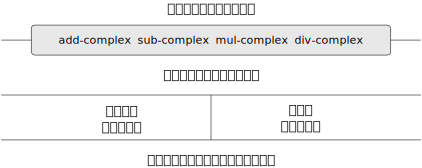
\includegraphics[width=108mm]{fig/chap2/Fig2.19a.pdf}
\par\bigskip
\noindent
\heading{図2.19:} 複素数システムのデータ抽象化の壁
\end{figure}

\link{2.5節}では、タイプタグとデータ主導スタイルを使ってジェネリック算術演算
パッケージを開発するやり方を示します。このシステムは、すべての種類の``数値''を操作
するのに使える手続き(\code{add}, \code{mul} など)を提供し、新たな種類の数値が必要に
なったら簡単に拡張できるようになっています。\link{2.5.3節}では、記号代数を実行
するシステムの中でジェネリック数値演算を使う方法を示します。

\subsection{複素数の表現}
\label{2.4.1節}
\label{Sec. 2.4.1}

ここでは、ジェネリック演算を使うプログラムの単純で非現実的な例として、複素数に対する
算術演算を行うシステムを開発していきます。まず、複素数を順序つきペアとして表すときに
考えられる二つの表現方法、直交形式(実部と虚部)と極形式(絶対値と偏角)について検討します。
\footnote{実際の計算システムでは、ほとんどの場合、直交形式が選ばれます。
これは、直交形式と極形式の変換時に発生する丸め誤差のためです。このため、この
複素数の例は現実的ではありません。しかし、ジェネリック演算を使ったシステムの
設計を説明する例としては明快ですし、この章の後のほうで開発する、より実質的な
システムへの導入としても役に立ちます。}
\link{2.4.2節}では、タイプタグとジェネリック演算を使うことによって両方の表現を
共存させるやり方を示します。

有理数と同じように、複素数は順序つきペアとして自然に表現できます。複素数の集合は、
``実''軸と``虚''軸という二つの直交する軸を持つ二次元空間と考えることができます
(\link{図2.20}参照)。この見方をすると、\( z = x + iy \) (\( i^2 = -1 \))という
複素数は、実座標が\( x \)で虚座標が\( y \)の平面上の点として考えることができます。
複素数の和は、この表現では、座標の和になります。
\begin{comment}

\begin{example}
Real-part(z_1 + z_2) = Real-part(z_1) + Real-part(z_2)

Imaginary-part(z_1 + z_2) = Imaginary-part(z_1) + Imaginary-part(z_2)
\end{example}

\end{comment}
\begin{displaymath}
%  \eqalign{
% \hbox{Real-part} (z_1 + z_2)\; 		&=
% 	\hbox{ Real-part} (z_1)\; + \hbox{ Real-part} (z_2), \cr
% \hbox{Imaginary-part} (z_1 + z_2)\; 	&=
% 	\hbox{ Imaginary-part} (z_1)\; + \hbox{ Imaginary-part} (z_2). \cr
% } 
\begin{array}{r@{{}={}}l}
  \hbox{実部} (z_1 + z_2)\; 	&
	\hbox{ 実部} (z_1)\; + \hbox{ 実部} (z_2), \\
  \hbox{虚部} (z_1 + z_2)\; 	&
	\hbox{ 虚部} (z_1)\; + \hbox{ 虚部} (z_2).
\end{array}
\end{displaymath}

\begin{figure}[tb]
\phantomsection\label{図2.20}
\centering
\begin{comment}
\heading{図2.20:} Complex numbers as points in the plane.

\begin{example}
 Imaginary
    ^
    |
  y |.........................* z = x + ?y = r e^(?A)
    |                    __-- .
    |                __--     .
    |          r __--         .
    |        __--             .
    |    __-- \               .
    |__--    A |              .
----+----------+-------------------> Real
                              x
\end{example}
\end{comment}
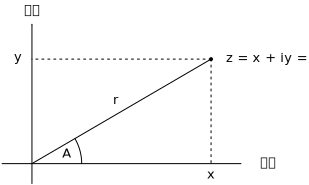
\includegraphics[width=79mm]{fig/chap2/Fig2.20.pdf}
\par\bigskip
\noindent
\heading{図2.20:} 平面上の点としての複素数
\end{figure}

複素数をかけ算するときには、複素数を極形式で、つまり大きさと角度(
\link{図2.20}内の\( r \)と\( A \))を使って考えるほうが自然です。
二つの複素数の積は、ひとつの複素数をもう一方の長さをかけて伸縮させ、
もう一方の角度だけ回転させて得られるベクトルになります。

\begin{comment}

\begin{example}
Magnitude(z_1 * z_2) = Magnitude(z_1) * Magnitude(z_2)

Angle(z_1 * z_2) = Angle(z_1) + Angle(z_2)
\end{example}

\end{comment}
\begin{displaymath}
%  \eqalign{
% 	\hbox{Magnitude} (z_1 \cdot z_2)\; 	&=
% 		\hbox{ Magnitude} (z_1)\; \cdot \hbox{ Magnitude} (z_2), \cr
% 	\hbox{Angle} (z_1 \cdot z_2)\; 		&=
% 		\hbox{ Angle} (z_1)\; + \hbox{ Angle} (z_2). \cr
% } 
\begin{array}{r@{{}={}}l}
	\hbox{大きさ} (z_1 \cdot z_2)\; 	&
		\hbox{ 大きさ} (z_1)\; \cdot \hbox{ 大きさ} (z_2), \\
	\hbox{角度} (z_1 \cdot z_2)\; 		&
		\hbox{ 角度} (z_1)\; + \hbox{ 角度} (z_2).
\end{array}
\end{displaymath}
つまり、複素数には二つの異なる表現があり、それぞれ異なる演算に適しているということです。
しかし、複素数を使うプログラムを書いている人の視点からは、データ抽象化の原則により、
コンピュータがどちらの表現を使っていても、複素数の演算すべてが使えるようになって
いなければいけません。例えば、直交形式によって指定された複素数の絶対値が求められると
便利なことがよくあります。同じように、極形式によって指定された複素数の実部を求められると
便利なことがよくあります。

そのようなシステムを設計するにあたっては、\link{2.1.1節}で有理数パッケージを
設計する際に使ったのと同じデータ抽象化戦略が使えます。複素数演算は、\code{real\-/part},
\code{imag\-/part}, \code{magnitude}, \code{angle}という四つのセレクタによって実装されて
いるとします。また、複素数の構築には二つの手続きがあるとします。
\code{make\-/from\-/real\-/imag}は、指定された実部と虚部を持つ複素数を返し、
\code{make\-/from\-/mag\-/ang}は、指定された絶対値と偏角を持つ複素数を返します。
これらの手続きは、任意の複素数に対して

\begin{scheme}
(make-from-real-imag (real-part z) (imag-part z))
\end{scheme}

\noindent
と

\begin{scheme}
(make-from-mag-ang (magnitude z) (angle z))
\end{scheme}

\noindent
の両方とも\code{z}に等しい複素数を返すという性質を持っています。


これらのコンストラクタとセレクタを使うことで、\link{2.1.1節}で有理数について
行ったように、コンストラクタとセレクタによって規定される``抽象データ''を使って
複素数の算術演算を実装できます。上の式に示したように、足し算と引き算は
実部と虚部を使って、またかけ算と割り算は絶対値と偏角を使って行えます。

\begin{scheme}
(define (add-complex z1 z2)
  (make-from-real-imag (+ (real-part z1) (real-part z2))
                       (+ (imag-part z1) (imag-part z2))))
(define (sub-complex z1 z2)
  (make-from-real-imag (- (real-part z1) (real-part z2))
                       (- (imag-part z1) (imag-part z2))))
(define (mul-complex z1 z2)
  (make-from-mag-ang (* (magnitude z1) (magnitude z2))
                     (+ (angle z1) (angle z2))))
(define (div-complex z1 z2)
  (make-from-mag-ang (/ (magnitude z1) (magnitude z2))
                     (- (angle z1) (angle z2))))
\end{scheme}

\noindent
複素数パッケージを完成させるには、複素数の表現を選び、コンストラクタとセレクタを
基本数値と基本リストを使って実装しなければいけません。すぐわかるように、この方法は
二通りあります。``直交形式''のペア(実部、虚部)として表現するか、``極形式''のペア
(絶対値、偏角)として表現するかです。どちらを選ぶべきでしょうか。

この二つの選択の具体的な例として、Ben BitdiddleとAlyssa P. Hackerという、独立に
複素数システムの表現を設計している二人のプログラマがいると想像してください。Ben は
複素数を直交形式で表現することにします。この場合、複素数の実部と虚部を選択することや、
複素数を与えられた実部と虚部から構築することは、素直に実現できます。絶対値と偏角を
求めたり、複素数を与えられた絶対値と偏角から構築するのは、次のような三角法の関係を
使います。
\begin{comment}

\begin{example}
                      __________
x = r cos A     r = ./ x^2 + y^2

y = r sin A     A = arctan(y,x)
\end{example}

\end{comment}
\begin{displaymath}
%  \eqalign{
% 	x = r \cos A, \qquad 	& r = \sqrt{x^2 + y^2}, \cr
% 	y = r \sin A, \qquad 	& A = \arctan(y, x), \cr
% } 
\begin{array}{r@{{}={}}lr@{{}={}}l}
	x & r \cos A, \qquad 	& r & \sqrt{x^2 + y^2}, \\
	y & r \sin A, \qquad 	& A & \arctan(y, x),
\end{array}
\end{displaymath}
これは、実部と虚部\( (x, y) \)と絶対値と偏角\( (r, A) \)の関係を表しています。
\footnote{
ここで出てきた逆正接関数はSchemeの\code{atan}手続きで計算できるもので、引数
\( y, x \)を取り、正接が\( y / x \)となる角度を返すよう定義されています。
引数の符号によって角度の象限が決まります。}
このため、Benの表現は以下のようなセレクタとコンストラクタによって書くことができます。

\begin{scheme}
(define (real-part z) (car z))
(define (imag-part z) (cdr z))
(define (magnitude z)
  (sqrt (+ (square (real-part z))
           (square (imag-part z)))))
(define (angle z)
  (atan (imag-part z) (real-part z)))
(define (make-from-real-imag x y) (cons x y))
(define (make-from-mag-ang r a)
  (cons (* r (cos a)) (* r (sin a))))
\end{scheme}

\noindent
一方、Alyssaは複素数を極形式で表現することにしました。彼女の方法では、絶対値と偏角の
セレクトは素直にできます。しかし、実部と虚部を求めるには、三角法の関係を使う必要が
あります。Alyssaの表現は次のようになります。

\begin{scheme}
(define (real-part z) (* (magnitude z) (cos (angle z))))
(define (imag-part z) (* (magnitude z) (sin (angle z))))
(define (magnitude z) (car z))
(define (angle z) (cdr z))
(define (make-from-real-imag x y)
  (cons (sqrt (+ (square x) (square y)))
        (atan y x)))
(define (make-from-mag-ang r a) (cons r a))
\end{scheme}

\noindent
データ抽象化の規律に従っているため、\code{add\-/complex}, \code{sub\-/complex},
\code{mul\-/complex}, \code{div\-/complex}の同じ実装が、Benの表現とAlyssaの表現の
どちらに対してもうまく動くということが保証されます。

\subsection{タグつきデータ}
\label{2.4.2節}

データ抽象化は、``最小責任の原則''の応用として見ることもできます。
\link{2.4.1節}で複素数システムを実装したとき、Benの直交形式による表現と
Alyssaの極形式による表現のどちらを使うこともできました。セレクタとコンストラクタが
抽象化の壁を作っているため、データオブジェクトの具体的な表現に何を選ぶかということを
最後の瞬間まで遅らせることができ、そのためシステム設計の柔軟性を最大限にできます。

最小責任の原則は、さらに極限まで進めることができます。もし望むなら、セレクタと
コンストラクタを設計した``後''になっても表現を曖昧にしたままで、Benの表現と
Alyssaの表現の``両方''を使うようにすることもできます。しかし、両方の実装が
単独のシステムに含まれている場合、極形式のデータと直交形式のデータを区別するための
何らかの方法が必要になります。そうしないと、例えば(3, 4)というペアの\code{magnitude}
(\jnewterm{絶対値})を求めるよう言われた場合に、答えを(数値を直交形式と解釈して)5とするべきか
(数値を極形式と解釈して)3とするべきかわかりません。これを区別できるようにする
素直なやり方は、\jnewterm{タイプタグ}(\newterm{type tag})---\code{rectangular}または
\code{polar}という記号---を、それぞれの複素数の一部として含めるというものです。
こうすると、複素数を操作することが必要になったときに、どちらのセレクタを適用するべきかを
このタグを使って決めることができます。

タグつきデータを操作するために、\code{type\-/tag}と\code{contents}という手続きを
持っていると想定します。\code{type\-/tag}はデータオブジェクトからタグを抽出するもので、
\code{contents}は実際の中身(複素数の場合、極形式または直交形式の座標)を抽出するものです。
また、\code{attach\-/tag}という手続きも持っていると仮定します。これは、タグと中身を取り、
タグつきデータオブジェクトを返すというものです。これを実装する素直なやり方は、普通の
リスト構造を使うというものです。

\begin{scheme}
(define (attach-tag type-tag contents)
  (cons type-tag contents))
(define (type-tag datum)
  (if (pair? datum)
      (car datum)
      (error "Bad tagged datum: TYPE-TAG" datum)))
(define (contents datum)
  (if (pair? datum)
      (cdr datum)
      (error "Bad tagged datum: CONTENTS" datum)))
\end{scheme}

\noindent
これらの手続きを使って、直交形式と極形式をそれぞれ識別する述語\code{rectangular?},
\code{polar?}を定義できます。

\begin{scheme}
(define (rectangular? z)
  (eq? (type-tag z) 'rectangular))
(define (polar? z) (eq? (type-tag z) 'polar))
\end{scheme}

\noindent
タイプタグを使うことにしたので、BenとAlyssaはコードを修正して、異なる表現が
同じシステムの中で共存できるようにしました。Benが複素数を構築するたびに、それに
直交形式というタグをつけます。Alyssaが複素数を構築するたびに、それに極形式という
タグをつけます。それに加えて、BenとAlyssaはそれぞれの手続きの名前が衝突しないように
しなければいけません。これを行う方法としては、Benが自分の表現の手続きに接尾辞
\code{rectangular}を追加し、Alyssaは自分の表現手続きに\code{polar}を追加するという
ものがあります。以下は、\link{2.4.1節}のBenの直交形式表現を修正したものです。

\begin{scheme}
(define (real-part-rectangular z) (car z))
(define (imag-part-rectangular z) (cdr z))
(define (magnitude-rectangular z)
  (sqrt (+ (square (real-part-rectangular z))
           (square (imag-part-rectangular z)))))
(define (angle-rectangular z)
  (atan (imag-part-rectangular z)
        (real-part-rectangular z)))
(define (make-from-real-imag-rectangular x y)
  (attach-tag 'rectangular (cons x y)))
(define (make-from-mag-ang-rectangular r a)
  (attach-tag 'rectangular
              (cons (* r (cos a)) (* r (sin a)))))
\end{scheme}

\noindent
Alyssaの極形式表現の修正版のは次のようになりました。

\begin{scheme}
(define (real-part-polar z)
  (* (magnitude-polar z) (cos (angle-polar z))))
(define (imag-part-polar z)
  (* (magnitude-polar z) (sin (angle-polar z))))
(define (magnitude-polar z) (car z))
(define (angle-polar z) (cdr z))
(define (make-from-real-imag-polar x y)
  (attach-tag 'polar
              (cons (sqrt (+ (square x) (square y)))
                    (atan y x))))
(define (make-from-mag-ang-polar r a)
  (attach-tag 'polar (cons r a)))
\end{scheme}

\noindent
どちらのジェネリックセレクタも、引数のタグをチェックして、そのタイプのデータを扱う
適切な手続きを呼ぶ手続きとして実装されています。例えば、複素数の実部を得る場合、
\code{real\-/part}はタグを調べ、Benの\code{real\-/part\-/rectangular}とAlyssaの
\code{real\-/part\-/polar}のどちらを使うのかを決定します。どちらの場合でも、
\code{contents}を使って生のタグなしデータを取り出し、それを必要に応じて直交形式または
極形式の手続きに渡します。

\begin{scheme}
(define (real-part z)
  (cond ((rectangular? z)
         (real-part-rectangular (contents z)))
        ((polar? z)
         (real-part-polar (contents z)))
        (else (error "Unknown type: REAL-PART" z))))
(define (imag-part z)
  (cond ((rectangular? z)
         (imag-part-rectangular (contents z)))
        ((polar? z)
         (imag-part-polar (contents z)))
        (else (error "Unknown type: IMAG-PART" z))))
(define (magnitude z)
  (cond ((rectangular? z)
         (magnitude-rectangular (contents z)))
        ((polar? z)
         (magnitude-polar (contents z)))
        (else (error "Unknown type: MAGNITUDE" z))))
(define (angle z)
  (cond ((rectangular? z)
         (angle-rectangular (contents z)))
        ((polar? z)
         (angle-polar (contents z)))
        (else (error "Unknown type: ANGLE" z))))
\end{scheme}

\noindent
複素数の算術演算を実装するのには、\link{2.4.1節}の手続き\code{add\-/complex}, 
\code{sub\-/complex}, \code{mul\-/complex}, \code{div\-/complex}と同じものが使えます。
それらが呼び出すセレクタはジェネリックなので、どちらの表現を使っても動くからです。
例えば、手続き\code{add\-/complex}は相変わらずそのままで、以下のようになります。

\begin{scheme}
(define (add-complex z1 z2)
  (make-from-real-imag (+ (real-part z1) (real-part z2))
                       (+ (imag-part z1) (imag-part z2))))
\end{scheme}

\noindent
最後に、複素数を構築するのにBenの表現とAlyssaの表現のどちらを使うかを決める必要が
あります。実部と虚部が渡されたときには直交形式を使い、大きさと角度を渡されたときには
極形式を使うというのが妥当でしょう。

\begin{scheme}
(define (make-from-real-imag x y)
  (make-from-real-imag-rectangular x y))
(define (make-from-mag-ang r a)
  (make-from-mag-ang-polar r a))
\end{scheme}

\noindent
このようにして作った複素数システムは、\link{図2.21}に示すような構造を持ちます。
システムは、比較的独立した三つの部分に分解されています。複素数算術演算、Alyssaの
極形式による実装、Benの直交形式による実装です。極形式と直交形式の実装は、Benと
Alyssaが別々に書いていたとしても問題ありません。第三者のプログラマが抽象コンストラクタ、
セレクタによって複素数算術演算手続きを実装する際に、内部表現として両方とも使うことが
できます。

\begin{figure}[tb]
\phantomsection\label{図2.21}
\centering
\begin{comment}
\begin{quote}
\heading{図2.21:} Structure of the generic complex-arithmetic system.

\begin{example}
    +-------------------------------------------------+
----| add-complex sub-complex mul-complex div-complex |----
    +-------------------------------------------------+
                Complex arithmetic package
                 +-----------------------+
                 | real-part   imag-part |
-----------------|                       |------------------
                 | magnitude   angle     |
                 +-----------+-----------+
           Rectangular       |          Polar
          representation     |     representation
-----------------------------+------------------------------
       List structure and primitive machine arithmetic
\end{example}
\end{quote}
\end{comment}
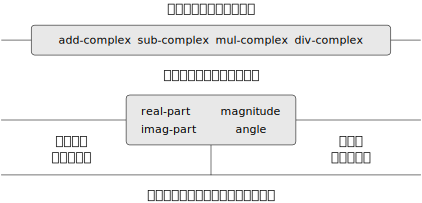
\includegraphics[width=108mm]{fig/chap2/Fig2.21a.pdf}
\par\bigskip
\noindent
\heading{図2.21:} ジェネリックな複素数算術演算システムの構造
\end{figure}

それぞれのデータオブジェクトには型のタグがついているので、セレクタはジェネリックに
データを操作します。つまり、それぞれのセレクタは適用されるデータの個々の型によって
異なるふるまいをするように定義されているということです。別々の表現をインターフェイスで
接続する際の一般的なメカニズムに注目してください。ある表現の実装(例えば、Alyssaの
極形式パッケージ)の中で極形式型の複素数を操作するときには、タグを取り除き、中身を
Alyssaのコードに渡します。逆に、Alyssaが一般使用のための数値を構築する際には、
それに型のタグをつけて、上のレベルの手続きが適切に認識できるようにします。データ
オブジェクトをレベル間でやりとりする際にタグをつけたり外したりするというこの規律は、
重要な組織化戦略になりえます。\link{2.5節}では、このことについて見ていきます。

\subsection{データ主導プログラミングと加法性}
\label{2.4.3節}

データの型をチェックし適切な手続きを呼ぶ一般的な戦略は\jnewterm{型によるディスパッチ}
(\newterm{dispatching on type})と呼ばれるものです。これは、システム設計でモジュール性を
達成するための強力な戦略です。一方で、\link{2.4.2節}のようにディスパッチを実装する
ことには二つの大きな弱点があります。弱点のひとつは、ジェネリックインターフェイス手続き
(\code{real\-/part}, \code{imag\-/part}, \code{magnitude}, \code{angle})がすべての異なる
表現について知っていなければいけないということです。例えば、複素数の新しい表現をこの複素数
システムに組み込みたいとします。そのためには、この新しい表現を型で識別できるようにして、
それから各ジェネリックインターフェイス手続きにその新しい型をチェックする節を追加し、
そしてその表現に対する適切なセレクタを適用することが必要になるでしょう。

このテクニックのもうひとつの弱点は、個々の表現は別々に設計できるものの、システム全体で
二つの手続きが同じ名前を持つということがないように保証しなければならないということです。
このために、BenとAlyssaは\link{2.4.1節}の元の手続きの名前を変える必要があったのでした。

この二つの弱点の元となっているのは、ジェネリックインターフェイスを実装するテクニックが
\jnewterm{加法的}(\newterm{additive})でないということです。ジェネリックセレクタ手続きを
実装する人は、新しい表現が組み込まれるたびにそれらの手続きを変更しなければならず、
また個々の表現のインターフェイスを作る人は、名前の衝突を避けるためにコードを変更しなければ
なりません。どちらの場合でも、コードに加えるべき変更は単純なものですが、それでもやはり
行わなければならず、このことが不便さとエラーの原因になります。これは複素数システムに
関しては現時点ではあまり大きな問題ではありませんが、仮に複素数の表現が二つではなく
数百個あったとしたらどうでしょうか。また、抽象データインターフェイスにはメンテナンスする
べきジェネリックセレクタが数多くあるとしたらどうでしょうか。また、すべてのインターフェイス
手続きやすべての表現について知っているプログラマが誰もいないとしたらどうでしょうか。
この問題は現実的なもので、大規模データベース管理システムのようなプログラムではこの問題に
取り組む必要があります。

ここで、システム設計をさらにモジュール化するための手段が必要になります。
\jnewterm{データ主導プログラミング}(\newterm{data-directed programming})として知られる
プログラミングテクニックはその手段を提供してくれます。データ主導プログラミングが
どうやって動くのかを理解するために、まず次のことに注目します。いろいろな型の集合に対して
共通のものとなるジェネリック演算を扱う際にはいつも、実質的には、ひとつの軸が可能な演算で、
もうひとつの軸が可能な型であるような二次元のテーブルを扱っていることになります。
テーブルの項目は、それぞれの引数の型に対するそれぞれの演算を実装する手続きです。
前の節で開発した複素数システムでは、演算の名前、データタイプ、実際の手続きの間の対応関係は、
ジェネリックインターフェイス手続きのいろいろな条件節の中に広がっていました。しかし、それと
同じ情報を\link{図2.22}に示すようにテーブルの中に構造化することもできたところです。

データ主導プログラミングは、そのようなテーブルを直接扱うようにプログラムを設計する
テクニックです。前のほうで、複素数算術演算のコードと、それぞれ型によって明示的な
ディスパッチを行う手続きの集合となっている二つの表現パッケージとの間の橋渡しをする
メカニズムを実装しました。ここでは、そのインターフェイス部分を、演算の名前と引数の型の
組み合わせをテーブルから検索して適用するべき正しい手続きを見つけ、それを引数の中身に
適用するということを行う、単一の手続きとして実装します。こうすると、新しい表現パッケージを
システムに追加する際に、既存の手続きには何の変更も加えなくても大丈夫です。テーブルに新しい
項目を追加するだけで十分です。

\begin{figure}[tb]
\phantomsection\label{図2.22}
\centering
\begin{comment}
\begin{quote}
\heading{図2.22:} Table of operations for the complex-number system.

\begin{example}
           |               Types
Operations | Polar           | Rectangular
===========+=================+======================
real-part  | real-part-polar | real-part-rectangular
imag-part  | imag-part-polar | imag-part-rectangular
magnitude  | magnitude-polar | magnitude-rectangular
angle      | angle-polar     | angle-rectangular
\end{example}
\end{quote}
\end{comment}
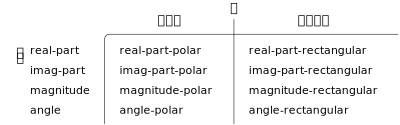
\includegraphics[width=102mm]{fig/chap2/Fig2.22.pdf}
\par\bigskip
\noindent
\heading{図2.22:} 複素数システム演算のテーブル
\end{figure}

この計画を実装するために、演算-型テーブルを操作する\code{put}と\code{get}という二つの
手続きがあるということにします。

\begin{itemize}

\item
\( \hbox{\tt(put}\;\langle \)\var{op}\( \kern0.1em\rangle\;\langle \)\var{type}\( \kern0.08em\rangle\;\langle \)\var{item}\( \kern0.08em\rangle\hbox{\tt)} \)は、テーブルの\( \langle \)\var{op}\( \kern0.1em\rangle \)と\( \langle \)\var{type}\( \kern0.08em\rangle \)が指すところに\( \langle \)\var{item}\( \kern0.08em\rangle \)を入れる。

\item
\( \hbox{\tt(get}\;\langle \)\var{op}\( \kern0.1em\rangle\;\langle \)\var{type}\( \kern0.08em\rangle\hbox{\tt)} \)は、テーブルから
\( \langle \)\var{op}\( \kern0.08em\rangle \), \( \langle \)\var{type}\( \kern0.08em\rangle \)の項目を検索し、そこで見つかった項目を返す。 見つからなければ、\code{get}はfalseを返す。

\end{itemize}

\noindent
今のところは、\code{put}と\code{get}は言語に含まれているということにします。
\link{第3章} (\link{3.3.3節})では、これらを含め、テーブル操作演算の実装方法
について学びます。

それでは、複素数システムでデータ主導プログラミングをどう使うかについて見ていきましょう。
直交形式表現を開発したBenは、元のものと同じようにコードを実装します。それから手続きの集合、
つまり\jnewterm{パッケージ}(\newterm{package})を定義し、システムに直交形式の数値の
扱い方を知らせるテーブルに項目を追加することで、これらの手続きをシステムのほかの部分と
接続します。これは、次の手続きを呼ぶことで行えます。

\begin{scheme}
(define (install-rectangular-package)
  ~\textrm{;; 内部手続き}~
  (define (real-part z) (car z))
  (define (imag-part z) (cdr z))
  (define (make-from-real-imag x y) (cons x y))
  (define (magnitude z)
    (sqrt (+ (square (real-part z))
             (square (imag-part z)))))
  (define (angle z)
    (atan (imag-part z) (real-part z)))
  (define (make-from-mag-ang r a)
    (cons (* r (cos a)) (* r (sin a))))

  ~\textrm{;; システムのほかの部分とのインターフェイス}~
  (define (tag x) (attach-tag 'rectangular x))
  (put 'real-part '(rectangular) real-part)
  (put 'imag-part '(rectangular) imag-part)
  (put 'magnitude '(rectangular) magnitude)
  (put 'angle '(rectangular) angle)
  (put 'make-from-real-imag 'rectangular
       (lambda (x y) (tag (make-from-real-imag x y))))
  (put 'make-from-mag-ang 'rectangular
       (lambda (r a) (tag (make-from-mag-ang r a))))
  'done)
\end{scheme}

\noindent
ここでの内部手続きが、\link{2.4.1節}でBenが単独で書いたものと同じ
手続きであることに注目してください。これらをシステムのほかの部分と接続するのに、
変更を加える必要はありません。それに、これらの手続きの定義は組み込み手続きの内部に
あるので、直交形式パッケージの外のほかの手続きと名前が衝突する心配もありません。
これらの手続きをシステムのほかの部分と接続するために、Benは自分の\code{real\-/part}
手続きを、演算名\code{real\-/part}と型\code{(rectangular)}のところに入れます。
ほかのセレクタも同じようにします。
\footnote{
ここでは、\code{rectangular}という記号ではなく\code{(rectangular)}というリストを使い、
必ずしも同じ型であるとは限らない複数の引数を持つ手続きを持てるようにしています。}
このインターフェイスは、システムのほかの部分から使うためのコンストラクタも定義しています。
\footnote{
コンストラクタを入れる場所の型はリストにしなくても大丈夫です。コンストラクタは必ず
ある特定の型のオブジェクトを作るのに使われるからです。}コンストラクタはBenが内部で
定義していたものと同じですが、タグをつけるというところが違います。

Alyassaの極形式パッケージも似たようなものになります。

\begin{scheme}
(define (install-polar-package)
  ~\textrm{;; 内部手続き}~
  (define (magnitude z) (car z))
  (define (angle z) (cdr z))
  (define (make-from-mag-ang r a) (cons r a))
  (define (real-part z) (* (magnitude z) (cos (angle z))))
  (define (imag-part z) (* (magnitude z) (sin (angle z))))
  (define (make-from-real-imag x y)
    (cons (sqrt (+ (square x) (square y)))
          (atan y x)))
  ~\textrm{;; システムのほかの部分とのインターフェイス}~
  (define (tag x) (attach-tag 'polar x))
  (put 'real-part '(polar) real-part)
  (put 'imag-part '(polar) imag-part)
  (put 'magnitude '(polar) magnitude)
  (put 'angle '(polar) angle)
  (put 'make-from-real-imag 'polar
       (lambda (x y) (tag (make-from-real-imag x y))))
  (put 'make-from-mag-ang 'polar
       (lambda (r a) (tag (make-from-mag-ang r a))))
  'done)
\end{scheme}

\noindent
BenとAlyssaは、相手のものと同じ名前(例えば、\code{real\-/part}など)によって
定義された元々の手続きをまだ使っていますが、これらの定義は今では別々の手続きの
内部定義(\link{1.1.8節}参照)になっているので、名前の衝突は起こりません。

複素数算術演算セレクタは、\code{apply\-/generic}というジェネリック``演算''手続きを
使ってテーブルにアクセスします。これは、ジェネリック演算を引数に適用するものです。
\code{apply\-/generic}は、テーブルから演算の名前と引数の型に対応する箇所を検索し、
手続きがあればそれを適用します。
\footnote{
\code{apply\-/generic}は、\link{練習問題 2.20}で説明したドット末尾記法を使います。
それぞれのジェネリック演算が取る引数の数は違うかもしれないからです。
\code{apply\-/generic}では、\code{op}は\code{apply\-/generic}の第一引数を値として
持ち、\code{args}は残りの引数のリストを値として持ちます。

また、\code{apply\-/generic}は\code{apply}という基本手続きを使っています。この手続きは
手続きとリストという二つの引数を取り、リストの要素を引数として手続きを適用します。
例えば、

\begin{smallscheme}
(apply + (list 1 2 3 4))
\end{smallscheme}

\noindent
は10を返します。}

\begin{scheme}
(define (apply-generic op . args)
  (let ((type-tags (map type-tag args)))
    (let ((proc (get op type-tags)))
      (if proc
          (apply proc (map contents args))
          (error
            "No method for these types: APPLY-GENERIC"
            (list op type-tags))))))
\end{scheme}

\noindent
\code{apply\-/generic}を使うと、複素数演算のジェネリックセレクタは以下のように定義
できます。

\begin{scheme}
(define (real-part z) (apply-generic 'real-part z))
(define (imag-part z) (apply-generic 'imag-part z))
(define (magnitude z) (apply-generic 'magnitude z))
(define (angle z) (apply-generic 'angle z))
\end{scheme}

\noindent
新しい表現がシステムに追加されてもこれらはまったく変わらないということに注意して
ください。

また、このパッケージの外部のプログラムが、実部と虚部や絶対値と偏角から複素数を作る際に
使うコンストラクタを抽出することもできます。\link{2.4.2節}と同じように、実部と
虚部がある場合は直交形式の複素数を構築し、絶対値と偏角がある場合は極形式の複素数を
構築します。

\begin{scheme}
(define (make-from-real-imag x y)
  ((get 'make-from-real-imag 'rectangular) x y))
(define (make-from-mag-ang r a)
  ((get 'make-from-mag-ang 'polar) r a))
\end{scheme}

\begin{quote}
\heading{\phantomsection\label{練習問題 2.73}練習問題 2.73:} 
\link{2.3.2節}では、記号微分を行うプログラムについて説明した。

\begin{scheme}
(define (deriv exp var)
  (cond ((number? exp) 0)
        ((variable? exp)
         (if (same-variable? exp var) 1 0))
        ((sum? exp)
         (make-sum (deriv (addend exp) var)
                   (deriv (augend exp) var)))
        ((product? exp)
         (make-sum (make-product
                    (multiplier exp)
                    (deriv (multiplicand exp) var))
                   (make-product
                    (deriv (multiplier exp) var)
                    (multiplicand exp))))
        ~\( \dark \langle \)~~\var{\dark more rules can be added here}~~\( \dark \rangle \)~
        (else (error "unknown expression type:
                      DERIV" exp))))
\end{scheme}

このプログラムは、微分する式の型によってディスパッチを実行していると捉えることもできる。
この場合、データの``タイプタグ''は代数演算記号(\code{+}など)で、行う演算は\code{deriv}
ということになる。基本的な微分を行う手続きを次のように書き直すと、プログラムを
データ主導スタイルに変形できる。

\begin{scheme}
(define (deriv exp var)
  (cond ((number? exp) 0)
        ((variable? exp) (if (same-variable? exp var) 1 0))
        (else ((get 'deriv (operator exp))
               (operands exp) var))))
(define (operator exp) (car exp))
(define (operands exp) (cdr exp))
\end{scheme}

\begin{enumerate}[a.]

\item
上で何をしているか説明せよ。手続き\code{number?}と\code{variable?}は、なぜデータ主導
ディスパッチとして取り込むことができないのだろうか。

\item
和と積に対する微分手続きと、上記のプログラムで使っているテーブルにそれらを組み込む
補助コードを書け。

\item
任意の微分規則(例えば、\link{練習問題 2.56}の指数の微分など)を選び、それを
このデータ主導システムに組み込め。

\item
この単純な代数操作では、式の型は式をまとめる代数演算子となっている。しかし、
仮に手続きのインデックスを逆にして、\code{deriv}でディスパッチを行う箇所を
次のようにするとする。
\begin{scheme}
((get (operator exp) 'deriv) (operands exp) var)
\end{scheme}

\noindent
これに対応して、微分システムにはどのような変更を加える必要があるだろうか。

\end{enumerate}
\end{quote}

\begin{quote}
\heading{\phantomsection\label{練習問題 2.74}練習問題 2.74:} 
Insatiable Enterprises, Inc.(貪欲エンタープライズ社)は、世界中に散らばった多数の
独立事業所からなる分散型複合企業である。この会社のコンピュータ設備は、どのユーザから
見てもネットワーク全体がひとつのコンピュータのように見えるような巧妙なネットワーク
インターフェイス方式によって相互接続されたところだ。貪欲社の社長は、初めてネットワークの
機能を使って事業所ファイルから管理情報を取り出そうとして愕然とした。事務所ファイルは
すべてSchemeのデータ構造として実装されているのに、使われている個々のデータ構造は
事業所ごとに違うのだ。事業所長会議が急遽開かれ、事業所の独立性をこれまで通りに保ったままで、
本部の要求を満たせるようにファイルを統合する戦略を探ることになった。

そのような戦略をデータ主導プログラミングによって実装する方法を示せ。例として、
各事業所の人事記録は単独のファイルからなり、従業員の名前をキーとしたレコードの集合を
持っているとする。集合の構造は事業所ごとに異なる。さらに、各従業員のレコードは
それ自身が(事業所ごとに異なる構造を持つ)集合で、\code{address}と\code{salary}のような
識別子をキーとした情報を含んでいるとする。具体的には、

\begin{enumerate}[a.]

\item
指定した人事ファイルから指定した従業員のレコードを取得する\code{get\-/record}手続きを
本部向けに実装せよ。この手続きは、任意の事業所のファイルに適用できる必要がある。
個々の事業所のファイルはどのように構造化しなければならないか説明せよ。具体的には、
どのような型情報を提供する必要があるだろうか。

\item
任意の事業所の人事ファイル内の与えられた職員のレコードから給与情報を返す\code{get\-/salary}
手続きを本部向けに実装せよ。この演算が動くようにするには、レコードはどのように構造化
しなければならないだろうか。

\item
本部向けに、\code{find\-/employee\-/record}手続きを実装せよ。この手続きは、全事業所の
ファイルから与えられた従業員を検索し、該当レコードを返す。引数として、従業員名と
全事業所のファイルのリストを取るとせよ。

\item
貪欲社が新しい会社を吸収した場合、新しい人事情報を中央システムに組み入れるためには
どのような変更が必要になるだろうか。

\end{enumerate}
\end{quote}

\subsubsection*{メッセージパッシング}

データ主導プログラミングでポイントとなる考え方は、プログラム中のジェネリック演算を
\link{図2.22}のような演算-型テーブルによって明示的に扱うというところです。
\link{2.4.2節}で使ったプログラミングスタイルでは、それぞれの演算に自分の
ディスパッチの面倒を見させることによって、必要となる型ディスパッチを構築していました。
実質的には、それぞれのジェネリック演算手続きがテーブルの行を表すというやり方で、
演算-型テーブルを行に分解していたことになります。

もうひとつの実装戦略は、テーブルを列に分解し、データ型によってディスパッチを行う
``賢い演算''を使うのではなく、演算の名前によってディスパッチを行う
``賢いデータオブジェクト''を使うというものです。これを実現するには、データオブジェクト
(例えば直交形式の複素数)を手続きとして表現し、その手続きは実行するべき演算名を引数として
取り、指定された演算を実行するというようにします。このような規律に従うと、
\code{make\-/from\-/real\-/imag}は以下のように書くことができます。

\begin{scheme}
(define (make-from-real-imag x y)
  (define (dispatch op)
    (cond ((eq? op 'real-part) x)
          ((eq? op 'imag-part) y)
          ((eq? op 'magnitude) (sqrt (+ (square x) (square y))))
          ((eq? op 'angle) (atan y x))
          (else (error "Unknown op: MAKE-FROM-REAL-IMAG" op))))
  dispatch)
\end{scheme}

\noindent
\code{apply\-/generic}手続きはジェネリック演算を引数に適用するものでしたが、
このデータに対応する\code{apply\-/generic}手続きは、単に演算の名前をデータオブジェクトに
渡して、オブジェクトに仕事をさせるだけになります。
\footnote{
この仕組みの制約のひとつは、一引数のジェネリック手続きしか使えないということです。
}

\begin{scheme}
(define (apply-generic op arg) (arg op))
\end{scheme}

\noindent
\code{make\-/from\-/real\-/imag}の返す値が手続き---内部手続き\code{dispatch}---である
ことに注意してください。これは、\code{apply\-/generic}が演算の実行を要求したときに
呼び出される手続きです。



このプログラミングスタイルは\jnewterm{メッセージパッシング}(\newterm{message passing})と
呼ばれています。この名前は、データオブジェクトは要求された演算の名前を``メッセージ''として
受け取る実体であるというイメージから来ています。メッセージパッシングの例については、
\link{2.1.3節}ですでに見ています。そこでは、\code{cons}, \code{car}, \code{cdr}が
データオブジェクトを使わずに手続きだけを使って定義できるということを見てきました。
ここでは、メッセージパッシングがただの数学的トリックではなく、ジェネリック演算によって
システムを組み立てるうえでの便利な技術だということを示しました。この章の残りでは、
ジェネリックな算術演算について検討するために、メッセージパッシングではなくデータ主導
プログラミングを使い続けることにします。\link{第3章}ではメッセージパッシングに戻り、
それがシミュレーションプログラムを構築するうえでの強力なツールになるということを見て
いきます。

\begin{quote}
\heading{\phantomsection\label{練習問題 2.75}練習問題 2.75:} 
コンストラクタ\code{make\-/from\-/mag\-/ang}をメッセージパッシングスタイルで実装せよ。
この手続きは、上で与えた\code{make\-/from\-/real\-/imag}と似たようなものになるだろう。
\end{quote}

\begin{quote}
\heading{\phantomsection\label{練習問題 2.76}練習問題 2.76:} 
ジェネリック演算を使った大きなシステムが発展するにつれ、新しいデータオブジェクトの型や
新しい演算が必要になることがある。三つの戦略(明示的ディスパッチによるジェネリック演算、
データ主導スタイル、メッセージパッシングスタイル)それぞれについて、新しい型や新しい
演算を追加するために必要な変更を記述せよ。新しい型がよく追加されるシステムでは、どの
どの組み立て方が最も適しているだろうか。新しい演算を追加するシステムでは、どれが最も
適しているだろうか。
\end{quote}

\section{ジェネリック演算によるシステム}
\label{2.5節}

前の節では、データオブジェクトの表現が二通り以上あるシステムの設計方法について
見てきました。ポイントとなる考え方は、ジェネリックインターフェイスという手段によって、
データ演算を指定するコードをいくつかの表現に結びつけるというものでした。ここでは、
同じ考え方を使って、いろいろな表現に対してジェネリックな演算を定義するだけでなく、
いろいろな種類の引数に対してジェネリックな演算を定義するやり方について見ていきます。
ここまで、いくつもの算術演算パッケージに触れてきました。言語組み込みの基本算術演算
(\code{+}, \code{-}, \code{*}, \code{/})、\link{2.1.1節}の有理数演算
(\code{add\-/rat}, \code{sub\-/rat}, \code{mul\-/rat}, \code{div\-/rat})、
それに\link{2.4.3節}で実装した複素数演算があります。今度はデータ主導テクニックを
使い、これまでに構築してきたすべての算術演算パッケージを合併した算術演算パッケージを
構築します。

\begin{figure}[tb]
\phantomsection\label{図2.23}
\centering
\begin{comment}
\label{図2.23}
\heading{図2.23:} Generic arithmetic system.

\begin{example}
                        Programs that use numbers
                           +-----------------+
---------------------------| add sub mul div |-------------------
                           +-----------------+
                        Generic arithmetic package
 +-----------------+   +-------------------------+
 | add-rat sub-rat |   | add-complex sub-complex |   +---------+
-|                 |-+-|                         |-+-| + - * / |-
 | mul-rat div-rat | | | mul-complex div-complex | | +---------+
 +-----------------+ | +-------------------------+ |
      Rational       |     Complex artithmetic     |   Ordinary
     arithmetic      +--------------+--------------+  arithmetic
                     | Rectangular  |     Polar    |
---------------------+--------------+--------------+-------------
             List structure and primitive machine arithmetic
\end{example}
\end{comment}
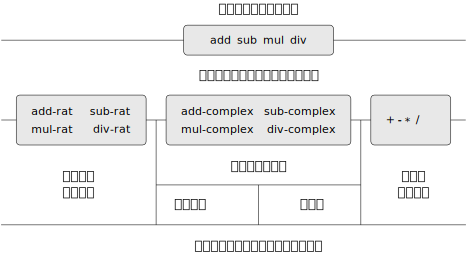
\includegraphics[width=111mm]{fig/chap2/Fig2.23a.pdf}
\par\bigskip
\noindent
\heading{図2.23:} ジェネリック算術演算システム
\end{figure}

\link{図2.23}は、これから構築するシステムの構造を示しています。抽象化の壁に
注目してください。``数値''を使う人の視点からは、どんな種類の数が与えられても演算を
行う\code{add}というたったひとつの手続きだけが見えています。\code{add}はジェネリック
インターフェイスの一部で、別々になっている通常の算術演算、有理数の算術演算、複素数の
算術演算のパッケージに、数値を使うプログラムから統一的なアクセスができるようにします。
個々の算術演算パッケージ(例えば複素数パッケージ)は、それ自身、異なる表現
(例えば直交形式と極形式)のために設計された複数のパッケージを連結するジェネリック手続き
(例えば\code{add\-/complex})によってアクセスするようになっていることもあります。
また、システムの構造は加法的なので、それぞれの算術演算パッケージは別々に設計して
組み合わせてジェネリック算術演算システムを作れるようになっています。

\subsection{ジェネリック算術演算}
\label{2.5.1節}


ジェネリック算術演算を設計するというタスクは、ジェネリック複素数演算を設計するのと
似たようなものになります。例えば、通常の数値に対しては基本手続きの足し算\code{+}の
ようにふるまい、有理数に対しては\code{add\-/rat}のようにふるまい、複素数に対しては
\code{add\-/complex}のようにふるまうジェネリックな足し算手続き\code{add}がほしい
ところです。\code{add}その他のジェネリック算術演算は、\link{2.4.3節}で複素数の
ジェネリックなセレクタの実装に使ったのと同じ戦略によって実装できます。それぞれの
種類の数値にタイプタグをくっつけ、ジェネリック手続きが引数のデータ型によって適切な
パッケージにディスパッチを行うようにします。

ジェネリック算術演算手続きは、次のように定義します。

\begin{scheme}
(define (add x y) (apply-generic 'add x y))
(define (sub x y) (apply-generic 'sub x y))
(define (mul x y) (apply-generic 'mul x y))
(define (div x y) (apply-generic 'div x y))
\end{scheme}

\noindent
まず、\jnewterm{通常の}(\newterm{ordinary})数値、つまり言語の基本数値を扱うパッケージを
組み込みます。通常の数値には\code{scheme\-/number}という記号のタグをつけることにします。
このパッケージの算術演算は基本算術演算手続きです(つまり、タグなし数値を扱うのに新たに
手続きを定義する必要はありません)。これらの演算はそれぞれ二つの引数を取るので、テーブルには
\code{(scheme\-/number scheme\-/number)}というリストをキーとして組み込みます。

\begin{scheme}
(define (install-scheme-number-package)
  (define (tag x) (attach-tag 'scheme-number x))
  (put 'add '(scheme-number scheme-number)
       (lambda (x y) (tag (+ x y))))
  (put 'sub '(scheme-number scheme-number)
       (lambda (x y) (tag (- x y))))
  (put 'mul '(scheme-number scheme-number)
       (lambda (x y) (tag (* x y))))
  (put 'div '(scheme-number scheme-number)
       (lambda (x y) (tag (/ x y))))
  (put 'make 'scheme-number (lambda (x) (tag x)))
  'done)
\end{scheme}

\noindent
scheme-numberパッケージのユーザは、次の手続きによって(タグつきの)通常の数値を作成します。

\begin{scheme}
(define (make-scheme-number n)
  ((get 'make 'scheme-number) n))
\end{scheme}

\noindent
ジェネリック算術演算システムの枠組みがもうできているので、新しい種類の数値を
加えることは簡単にできます。以下は、有理数算術演算を行うパッケージです。加法性のおかげで、
\link{2.1.1節}の有理数のコードを修正なしでパッケージの内部手続きとして使えるという
ところに注目してください。

\begin{scheme}
(define (install-rational-package)
  ~\textrm{;; 内部手続き}~
  (define (numer x) (car x))
  (define (denom x) (cdr x))
  (define (make-rat n d)
    (let ((g (gcd n d)))
      (cons (/ n g) (/ d g))))
  (define (add-rat x y)
    (make-rat (+ (* (numer x) (denom y))
                 (* (numer y) (denom x)))
              (* (denom x) (denom y))))
  (define (sub-rat x y)
    (make-rat (- (* (numer x) (denom y))
                 (* (numer y) (denom x)))
              (* (denom x) (denom y))))
  (define (mul-rat x y)
    (make-rat (* (numer x) (numer y))
              (* (denom x) (denom y))))
  (define (div-rat x y)
    (make-rat (* (numer x) (denom y))
              (* (denom x) (numer y))))
  ~\textrm{;; システムのほかの部分とのインターフェイス}~
  (define (tag x) (attach-tag 'rational x))
  (put 'add '(rational rational)
       (lambda (x y) (tag (add-rat x y))))
  (put 'sub '(rational rational)
       (lambda (x y) (tag (sub-rat x y))))
  (put 'mul '(rational rational)
       (lambda (x y) (tag (mul-rat x y))))
  (put 'div '(rational rational)
       (lambda (x y) (tag (div-rat x y))))
  (put 'make 'rational
       (lambda (n d) (tag (make-rat n d))))
  'done)
(define (make-rational n d)
  ((get 'make 'rational) n d))
\end{scheme}

\noindent
複素数を扱う同様のパッケージを、\code{complex}というタグを使って組み込みます。
このパッケージを作る際に、直交形式と極形式のパッケージで定義した演算
\code{make\-/from\-/real\-/imag}と\code{make\-/from\-/mag\-/ang}をテーブルから
取り出しています。加法性のおかげで、\link{2.4.1節}の手続き
\code{add\-/complex}, \code{sub\-/complex}, \code{mul\-/complex}, \code{div\-/complex}
が内部手続きとして使えます。

\begin{scheme}
(define (install-complex-package)
  ~\textrm{;; 直交形式パッケージと極形式パッケージからインポートした手続き}~
  (define (make-from-real-imag x y)
    ((get 'make-from-real-imag 'rectangular) x y))
  (define (make-from-mag-ang r a)
    ((get 'make-from-mag-ang 'polar) r a))
  ~\textrm{;; 内部手続き}~
  (define (add-complex z1 z2)
    (make-from-real-imag (+ (real-part z1) (real-part z2))
                         (+ (imag-part z1) (imag-part z2))))
  (define (sub-complex z1 z2)
    (make-from-real-imag (- (real-part z1) (real-part z2))
                         (- (imag-part z1) (imag-part z2))))
  (define (mul-complex z1 z2)
    (make-from-mag-ang (* (magnitude z1) (magnitude z2))
                       (+ (angle z1) (angle z2))))
  (define (div-complex z1 z2)
    (make-from-mag-ang (/ (magnitude z1) (magnitude z2))
                       (- (angle z1) (angle z2))))
  ~\textrm{;; システムのほかの部分とのインターフェイス}~
  (define (tag z) (attach-tag 'complex z))
  (put 'add '(complex complex)
       (lambda (z1 z2) (tag (add-complex z1 z2))))
  (put 'sub '(complex complex)
       (lambda (z1 z2) (tag (sub-complex z1 z2))))
  (put 'mul '(complex complex)
       (lambda (z1 z2) (tag (mul-complex z1 z2))))
  (put 'div '(complex complex)
       (lambda (z1 z2) (tag (div-complex z1 z2))))
  (put 'make-from-real-imag 'complex
       (lambda (x y) (tag (make-from-real-imag x y))))
  (put 'make-from-mag-ang 'complex
       (lambda (r a) (tag (make-from-mag-ang r a))))
  'done)
\end{scheme}

\noindent
複素数パッケージの外部のプログラムは、複素数を構築するのに実部と虚部を使うこともできますし、
絶対値と偏角を使うこともできます。元の手続きは、本来は直交形式パッケージと
極形式パッケージの中で定義されたものですが、そこから複素数パッケージにエクスポートされ、
さらにそこから外の世界へとエクスポートされているというところに注目してください。

\begin{scheme}
(define (make-complex-from-real-imag x y)
  ((get 'make-from-real-imag 'complex) x y))
(define (make-complex-from-mag-ang r a)
  ((get 'make-from-mag-ang 'complex) r a))
\end{scheme}

\noindent
ここでは、二つのレベルのタグシステムができています。\( 3 + 4i \)のような典型的な複素数は、
\link{図2.24}に示すように表現されることになります。外側のタグ(\code{complex})は、
数値を複素数パッケージに送るために使われます。複素数パッケージに入ると、次のタグ
数値を直交形式パッケージに送るのに(\code{rectangular})タグが使われます。
巨大で複雑なシステムでは、多くのレベルが、それぞれ次のレベルとジェネリック演算という
手段によって接続されるという形で存在するということがありえます。データオブジェクトが
``下向きに''渡されるにつれ、適切なパッケージに送るために使われた外側のタグは
(\code{contents}の適用によって)はがされ、(もしあれば)次のレベルのタグが
見えるようになり、さらなるディスパッチに使われます。

\begin{figure}[tb]
\phantomsection\label{図2.24}
\centering
\begin{comment}
\heading{図2.24:} Representation of \( 3 + 4i \) in rectangular form.

\begin{example}
     +---+---+     +---+---+     +---+---+
---->| * | *-+---->| * | *-+---->| * | * |
     +-|-+---+     +-|-+---+     +-|-+-|-+
       |             |             |   |
       V             V             V   V
 +---------+   +-------------+  +---+ +---+
 | complex |   | rectangular |  | 3 | | 4 |
 +---------+   +-------------+  +---+ +---+
\end{example}
\end{comment}
\includegraphics[width=64mm]{fig/chap2/Fig2.24c.pdf}
\par\bigskip
\noindent
\heading{図2.24:} 直交形式による\( 3 + 4i \)の表現
\end{figure}

上記のパッケージでは、\code{add\-/rat}, \code{add\-/complex}その他の算術演算手続きは、
最初に書いたときそのままの状態で使いました。しかし、これらの定義が異なるインストール
手続きの内部に入ると、互いに識別できる名前である必要はなくなります。両方のパッケージで、
単に\code{add}, \code{sub}, \code{mul}, \code{div}という名前をつけていたとしても大丈夫です。

\begin{quote}
\heading{\phantomsection\label{練習問題 2.77}練習問題 2.77:} 
Louis Reasonerは、式\code{(magnitude z)}を評価しようとした。ここで、\code{z}は
\link{図2.24}に示したオブジェクトである。驚いたことに、5という答えが返ってくるのでは
なく、\code{apply\-/generic}からのエラーメッセージが返ってきて、型\code{(complex)}には
\code{magnitude}という演算を行う手続きがないという。彼がこの対話をAlyssa P. Hackerに
見せると、Alyssaは``複素数セレクタが\code{polar}と\code{rectangular}の数値にだけしか
定義されていなくて、\code{complex}の数値に対して定義されていないのが問題なのよ。
動くようにするには\code{complex}パッケージに以下の式を追加すれば大丈夫''と言う。

\begin{scheme}
(put 'real-part '(complex) real-part)
(put 'imag-part '(complex) imag-part)
(put 'magnitude '(complex) magnitude)
(put 'angle '(complex) angle)
\end{scheme}

なぜこれが動くのか、詳しく説明せよ。例として、\code{z}が\link{図2.24}に示した
オブジェクトであるとき、式\code{(magnitude z)}を評価した際に呼ばれるすべての手続きを
トレースせよ。具体的には、\code{apply\-/generic}は何回起動されるだろうか。
それぞれの場合について、ディスパッチ先の手続きは何になるだろうか。
\end{quote}

\begin{quote}
\heading{\phantomsection\label{練習問題 2.78}練習問題 2.78:} 
\code{scheme\-/number}パッケージの内部手続きは、本質的に基本手続き\code{+}, \code{-}
その他に対する呼び出しでしかない。ここでのタイプタグシステムでは、各データオブジェクトに
型がくっついていないといけないようになっていたので、直接この言語の基本手続きを使う
ことはできなかった。しかし、実際のところ、Lisp の実装はすべて型システムを持っていて、
内部で使用している。\code{symbol?}や\code{number?}のような基本述語は、データオブジェクトが
特定の型を持つか識別している。\link{2.4.2節}の\code{type\-/tag}, \code{contents},
\code{attach\-/tag}の定義を変更し、ここでのジェネリックシステムがSchemeの内部型システムを
利用できるようにせよ。つまり、システムの挙動はそのままで、普通の数値を\code{car}が
\code{scheme\-/number}という記号であるペアとして表すのではなく、単にSchemeの数値として
表現されるようにせよ。
\end{quote}

\begin{quote}
\heading{\phantomsection\label{練習問題 2.79}練習問題 2.79:}
二つの数値の等価性をテストするジェネリックな等価性述語\code{equ?}を定義し、
ジェネリック算術演算パッケージに組み込め。この演算は、通常の数値、有理数、複素数に対して
動作しなければならない。
\end{quote}

\begin{quote}
\heading{\phantomsection\label{練習問題 2.80}練習問題 2.80:} 
引数が0であるかテストするジェネリックな述語\code{=zero?}を定義し、ジェネリック算術
演算パッケージに組み込め。この演算は、通常の数値、有理数、複素数に対して動作しなければ
ならない。
\end{quote}

\subsection{異なる型のデータを組み合わせる}
\label{2.5.2節}

ここまで、統合算術演算システムの定義の仕方について見てきました。このシステムは、
通常の数値、複素数、有理数を含み、またこのほかどんな数値のタイプでも作って組み込む
ことができるものでした。しかし、無視してきた重要な問題がひとつあります。ここまでで
定義してきた演算は、異なるデータ型を完全に独立したものとして扱うようになっています。
つまり、例えば二つの通常の数字を足すのと二つの複素数を足すのに別々のパッケージが
あるということです。考えの対象外にしていたのは、型の境界を超えた演算、例えば複素数と
通常の数値との足し算のようなものについて考えることに意味があるという事実です。
私たちは、プログラムの部品同士の間に壁を作り、独立して開発したり理解したりできるように
することに多大な労力をつぎ込んできました。ここでは、注意深くコントロールされた
やり方でクロスタイプ(異なる型同士)の演算を導入し、モジュール境界を大きく壊すことなく
それらの演算をサポートできるようにします。

クロスタイプ演算を扱う方法のひとつは、可能な型の組み合わせの中で、演算が有効であるもの
それぞれに対して別々の手続きを設計するというものです。例えば、複素数パッケージを拡張し、
複素数と実数の足し算を提供するようにして、\code{(complex scheme\-/number)}というタグを
使ってテーブルに組み込むということができます。
\footnote{このほかに、\code{(scheme\-/number complex)}という二つの型を扱うために、
ほとんど同じ手続きをもうひとつ用意する必要があります。}

\begin{scheme}
~\textrm{;; 複素数パッケージに含める}~
(define (add-complex-to-schemenum z x)
  (make-from-real-imag (+ (real-part z) x) (imag-part z)))
(put 'add '(complex scheme-number)
     (lambda (z x) (tag (add-complex-to-schemenum z x))))
\end{scheme}

\noindent
このテクニックはうまくいくのですが、面倒です。このようなシステムでは、新しい型を導入する
コストが、その型を扱う手続きのパッケージの構築だけでは終わらず、クロスタイプ演算を
実装する手続きを構築して組み込む分まで必要になります。これはあっという間に、その型自身の
演算を定義するのに必要な分よりずっと多い量になってしまいます。この手法はまた、別々の
パッケージを加法的に組み合わせる能力を台無しにしてしまいます。少なくとも、個々のパッケージを
実装する人がほかのパッケージについてあまり考慮しないでいいようにするという能力は台無しに
なってしまいます。例えば、上の例では、複素数と通常の数値の混合演算を扱うのが複素数
パッケージの責任だということは妥当に見えます。しかし、有理数と複素数を組み合わせるのは、
複素数パッケージでやってもいいし、有理数パッケージでやってもいいし、これら二つの
パッケージから演算を抽出する何らかの第三ののパッケージでやってもいいかもしれません。
複数のパッケージにわたる責任の分割について一貫したポリシーを策定するということは、
多くのパッケージと多くのクロスタイプ演算を伴うシステムを設計する際には、どうしようも
ないほど大変なタスクになってしまうでしょう。

\subsubsection*{強制型変換}

まったく関係のない型同士のまったく関連のない演算という一般的な状況では、
たとえ面倒でも、明示的なクロスタイプ演算を実装することぐらいしかできません。
幸い普通は、型システムに隠れているかもしれない積み上げ式の構造を利用して、
もっとうまくやることができます。別々のデータ型が完全に独立しているというわけでは
なく、ある型のオブジェクトをほかの型と見なす方法があるということはよくあります。
このプロセスは、\jnewterm{強制型変換}(\newterm{coercion})と呼ばれます。例えば、
通常の数値と複素数を算術演算によって組み合わせることを求められたら、通常の数値を
虚部がゼロの複素数と見なすことができます。こうすると、この問題を二つの複素数を
組み合わせる問題に変換でき、複素数パッケージによって普通のやり方で扱うことが
できるようになります。

一般に、ある型のオブジェクトを等価なほかの型のオブジェクトに変換する強制型変換手続きを
設計することによって、この考え方を実装できます。以下のものは典型的な強制型変換手続きで、
与えられた通常の数値を、実部がその数値で虚部がゼロの複素数に変換します。

\begin{scheme}
(define (scheme-number->complex n)
  (make-complex-from-real-imag (contents n) 0))
\end{scheme}

\noindent
これらの強制型変換手続きは、特別な強制型変換テーブルに組み込むことにします。
二つの型の名前をキーとして使います。

\begin{scheme}
(put-coercion 'scheme-number
              'complex
              scheme-number->complex)
\end{scheme}

\noindent
(このテーブルを操作するための手続き\code{put\-/coercion}と\code{get\-/coercion}が
存在すると仮定しています)一般に、このテーブルにはいくつか空きができます。
すべての型の任意のデータオブジェクトをほかのすべての型に強制型変換するということは、
一般的には可能でないからです。例えば、任意の複素数を実数に強制型変換する方法というものは
ありません。そのため、一般的な\code{complex\-/>scheme\-/number}手続きがテーブルに
含まれるということはありません。

強制型変換テーブルが準備できたら、\link{2.4.3節}の\code{apply\-/generic}手続きに
変更を加えることによって、強制型変換を統一的に扱うことができるようになります。演算を
適用することを求められたら、最初はこれまでと同じように引数の型に対して演算が定義されて
いるかどうかチェックします。定義されていれば、演算-型テーブルで見つかった手続きに
ディスパッチします。定義されていなければ、強制型変換を試みます。簡単にするために、
ここでは引数が二つの場合だけを考えます。\footnote{一般化については\link{練習問題 2.82}を
参照。}強制型変換テーブルを見て、一つ目の型のオブジェクトが二つ目の型に強制型変換可能か
どうか確認します。可能であれば、一つ目の引数を強制型変換し、もう一度演算を試みます。
もし一つ目の型のオブジェクトが二つ目の型に一般的に強制型変換できないのであれば、逆に
二つ目の引数を一つ目の引数の型に強制型変換できないか試してみます。最後に、どちらの型に
ついてももう一方の型に強制型変換する既知の方法がなければ、諦めます。手続きは以下のように
なります。

\begin{scheme}
(define (apply-generic op . args)
  (let ((type-tags (map type-tag args)))
    (let ((proc (get op type-tags)))
      (if proc
          (apply proc (map contents args))
          (if (= (length args) 2)
              (let ((type1 (car type-tags))
                    (type2 (cadr type-tags))
                    (a1 (car args))
                    (a2 (cadr args)))
                (let ((t1->t2 (get-coercion type1 type2))
                      (t2->t1 (get-coercion type2 type1)))
                  (cond (t1->t2
                         (apply-generic op (t1->t2 a1) a2))
                        (t2->t1
                         (apply-generic op a1 (t2->t1 a2)))
                        (else (error "No method for these types"
                                     (list op type-tags))))))
              (error "No method for these types"
                     (list op type-tags)))))))
\end{scheme}

\noindent
上でざっくり見たように、この強制型変換という構想は、明示的にクロスタイプ演算を定義する
という手法に比べて多くのメリットがあります。型同士を関連づけるために強制型変換手続きを
書く(\( n \)個の型を持つシステムに対しては、最大で\( n^2 \)個の手続き)ということはやはり
必要ですが、書く必要があるのはそれぞれの型のペアに対して手続きひとつだけで、それぞれの
型の集合とそれぞれのジェネリック演算に対して別々の手続きを書く必要はありません。
\footnote{うまくやると、普通は\( n^2 \)よりも少ない数の強制型変換手続きで済ませることが
できます。例えば、もし型1から型2への変換方法と型2から型3への変換方法がわかっていれば、
この知識を使って型1から型3に変換できます。このやり方を使うと、システムに
新しい型を追加する際に明示的に提供する必要のある強制型変換手続きの数を劇的に減らすことが
できます。もしシステムを必要なだけ高度なものにする準備があるのなら、システムが型同士の
関係の``グラフ''を検索して、明示的に提供された強制型変換手続きから推論できる強制型変換
手続きを自動的に生成させることもできます。}ここでは、型同士の適切な変換は型そのものによって
決まり、適用する演算には依存しないという事実を利用しています。

一方、この強制型変換構想の持つ汎用性では十分でない応用もあるかもしれません。組み合わせる
オブジェクトのどちらももう一方の型に変換できないという場合でも、両方のオブジェクトを
第三の型に変換することで演算の実行が可能かもしれません。そのような複雑な場合を扱いながら
プログラムのモジュール性を維持するためには、普通は型同士の関係のさらに深い構造を利用する
システムを構築することが必要になります。これについては次節で検討します。

\subsubsection*{型の階層}

上で紹介した強制型変換構想は、型のペアの間に自然な関係があるということを頼りにしていました。
しかし、異なる型の間の関係には、より``グローバルな''構造があるということがよくあります。
例えば、整数、有理数、実数、複素数を扱うジェネリック算術演算システムを構築していると
しましょう。そのようなシステムでは、整数を特別な種類の有理数と見なし、有理数を特別な種類の
実数と見なし、実数を特別な種類の複素数と見なすというのはとても自然です。ここで実際に扱って
いるのはいわゆる\jnewterm{型の階層}(\newterm{hierarchy of types})というもので、その中では、
例えば整数は有理数の\jnewterm{サブタイプ}(\newterm{subtype})(つまり、有理数に適用できる任意の
演算は自動的に整数に適用できる)ということになります。逆に、有理数は整数の\jnewterm{スーパータイプ}
(\newterm{supertype})と呼びます。ここで扱っている特定の階層はとても単純なもので、
それぞれの型は高々ひとつのスーパータイプと高々ひとつのサブタイプを持ちます。このような
構造は\jnewterm{タワー}(\newterm{tower})と呼ばれます。\link{図2.25}にこの構造を示します。

\begin{figure}[tb]
\phantomsection\label{図2.25}
\centering
\begin{comment}
\heading{図2.25:} A tower of types.

\begin{example}
 complex
   ^
   |
  real
   ^
   |
rational
   ^
   |
integer
\end{example}
\end{comment}
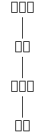
\includegraphics[width=11mm]{fig/chap2/Fig2.25.pdf}
\par\bigskip
\noindent
\heading{図2.25:} 型のタワー
\end{figure}

もし扱っているのがタワー構造であれば、階層に新しい型を追加するという問題はとても
簡単にできます。新しい型をすぐ上のスーパータイプに組み入れる方法と、新しい型が
すぐ下の型のどのようなスーパータイプであるかを記述するだけで十分だからです。
例えば、複素数と整数の足し算をしたい場合、明示的に\code{integer\-/>complex}
という特別な強制型変換手続きを定義する必要はありません。その代わりに、整数の
有理数への変換方法、有理数の実数への変換方法、実数の複素数への変換方法を定義します。
次に、システムがこれらのステップを通して整数を複素数に変換できるようにして、
それから二つの複素数を足し合わせます。

\code{apply\-/generic}手続きは、次のように設計し直すことができます。それぞれの型に
対して、その型のオブジェクトをタワーの一階上に``上げる''\code{raise}という手続きを用意
します。こうすると、システムが異なる型のオブジェクトの演算を行うよう求められたとき、
すべてのオブジェクトが塔の同じ階に揃うようになるまで低い型を連続して上げていくという
ことができるようになります(\link{練習問題 2.83}と\link{練習問題 2.84}は、そのような
戦略の実装の詳細に関係するものです)。

タワーの別の利点として、すべての型がスーパータイプに定義されたすべての演算を
``継承する''という概念を簡単に実装できるということがあります。例えば、整数に
対して実部を求める特別な手続きを提供していないとしても、整数は複素数のサブタイプ
なので、整数に対しても\code{real\-/part}が定義されていることが期待されます。
タワーであれば、\code{apply\-/generic}を修正して、統一的な方法でこれを実現できます。
もし必要な演算が与えられたオブジェクトの型に対して直接定義されていなければ、
オブジェクトをそのスーパータイプに上げて再試行します。こうやって、望む演算が実行可能に
なる階にたどり着くか、てっぺんに当たるか(その場合はあきらめることになります)するまで、
引数を変換しながらタワーを登っていきます。

より一般的な階層に対してのタワーのもう一つの利点は、データオブジェクトを最も単純な
表現に``下げる''ことが簡単にできるということがあります。例えば、\( 2 + 3i \)と
\( 4 - 3i \)を足す場合、複素数\( 6 + 0i \)という形で答えを得るよりも、整数の6という
答えを得るほうがいいでしょう。\link{練習問題 2.85}では、そのようなレベル下げ演算に
ついて検討します(注意すべきところは、レベル下げが可能な\( 6 + 0i \)のような
オブジェクトと、レベル下げが不可能な\( 6 + 2i \)のようなオブジェクトを見分ける
一般的な方法が必要だというところです)。

\subsubsection*{階層の不適切さ}

システムのデータ型が自然にタワーとして配置できる場合、ここまで見てきたように、
異なる型同士のジェネリック演算の問題はとても単純になります。残念ながら、
普通はそうはいきません。\link{図2.26} はいろいろな型のより複雑な関係を
図示したものです。この例では、さまざまな型の幾何学図形同士の関係を示しています。
この図から、一般的にはひとつの型が二つ以上のサブタイプを持つということが見て取れます。
例えば、三角形と四角形はどちらも多角形のサブタイプです。それに加えて、ひとつの型が
二つ以上のスーパータイプを持つこともあります。例えば、直角二等辺三角形は二等辺三角形と
見なすこともできますし、直角三角形と見なすこともできます。この複数スーパータイプ問題は
特に厄介です。ある型を階層の中で``上げる''ための唯一の方法というものがないということに
なるからです。あるオブジェクトにある演算を適用する際に、``正しい''スーパータイプを
見つけるために、\code{apply\-/generic}のような手続きが型ネットワーク全体の中を
かなり検索しないといけないことになるかもしれません。一般的に、ひとつの型には複数の
サブタイプがあるので、値を型階層の中で``下げる''強制型変換にも同じような問題があります。
巨大システムを設計する際に、モジュール性を保ちながら相互に関連する多くの型を取り扱う
ということは非常に難しく、現在多くの研究がなされている領域です。
\footnote{この文は第一版にもあったものですが、12年前と同じように、現状に対しても
当てはまります。いろいろな型を持つ実体同士の関係(哲学者が``オントロジー''と呼ぶもの)
を表現する実用的で汎用的な枠組みを開発するということは、どうしようもないほど
難しいように思えます。10年前に存在した混乱といま存在する混乱の主な違いは、今では
いろいろな不適切なオントロジーの理論が、同じように不適切なプログラミング言語の山に
組み入れられているということです。例えば、オブジェクト指向言語の複雑性---それと、
現代的なオブジェクト指向言語同士の微妙で混乱を招く相違点---の多くは、相互に関連する
型に対するジェネリック演算の扱いが中心となっています。\link{第3章}では計算
オブジェクトについて検討しますが、これらの問題を完全に回避しています。オブジェクト
指向言語に慣れた読者は、\link{第3章}で局所状態についてかなり紙面を費やして
いるのに、``クラス''や``継承''には一言も触れていないことに気づくと思います。
実際のところ、知識表現や自動推論の研究成果を利用することなしに、これらの問題を
コンピュータ言語設計という観点のみから解決することはできないのではないかと私たちは
疑っています。}

\begin{figure}[tb]
\phantomsection\label{図2.26}
\centering
\begin{comment}
\heading{図2.26:} Relations among types of geometric figures.

\begin{example}
                     polygon
                    /       \
                   /         \
            triangle         quadrilateral
            /     \              /     \
           /       \            /       \
     isosceles   right      trapezoid   kite
     triangle    triangle       |         |
      |     \      |            |         |
      |      \     |            |         |
equilateral   isosceles   parallelogram   |
triangle      right          |       \    |
              triangle       |        \   |
                          rectangle  rhombus
                                \    /
                                 \  /
                                square
\end{example}
\end{comment}
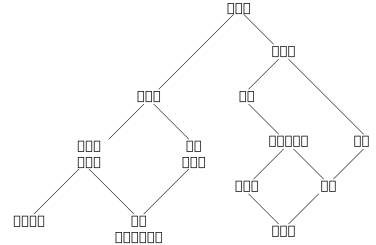
\includegraphics[width=96mm]{fig/chap2/Fig2.26e.pdf}
\par\bigskip
\noindent
\heading{図2.26:} 幾何学図形の型の間の関係
\end{figure}

\begin{quote}
\heading{\phantomsection\label{練習問題 2.81}練習問題 2.81:} 
Louis Reasonerは、引数の型がすでに同じであっても、\code{apply\-/generic}は引数を
お互いの型に強制型変換しようとしてもいいのではないかと気がついた。そのため、
それぞれの型の引数をそれ自身の型に\jnewterm{強制型変換}(\newterm{coerce})する
手続きを強制型変換テーブルに入れる必要があると彼は考えた。例えば、上に示した
\code{scheme\-/number\-/>complex}という強制型変換に加え、彼は次のことを行う。

\begin{scheme}
(define (scheme-number->scheme-number n) n)
(define (complex->complex z) z)
(put-coercion 'scheme-number
              'scheme-number
              scheme-number->scheme-number)
(put-coercion 'complex 'complex complex->complex)
\end{scheme}

\begin{enumerate}[a.]

\item
Louisの強制型変換手続きを組み込むと、もし\code{scheme\-/number}型の二つの引数や
\code{complex}型の二つの引数とある演算に対して\code{apply\-/generic}が呼ばれ、
その演算がテーブル内でそれらの型に対して見つからない場合は、何が起こるだろうか。
例えば、ジェネリックな指数関数演算を定義したとする。

\begin{scheme}
(define (exp x y) (apply-generic 'exp x y))
\end{scheme}

\noindent
そして、Scheme-numberパッケージに対して指数関数手続きを追加し、ほかのパッケージには
追加しないとする。

\begin{scheme}
~\textrm{;; 以下はScheme-numberパッケージに追加する}~
(put 'exp '(scheme-number scheme-number)
     (lambda (x y) (tag (expt x y))))
     ~\textrm{; 基本手続き\code{expt}を使う}~
\end{scheme}

\noindent
\code{exp}を二つの複素数の引数で呼び出した場合、何が起こるだろうか。

\item
同じ型の引数に対する強制型変換について手を加えないといけないとする
Louisの考え方は正しいだろうか。それとも、\code{apply\-/generic}はそのままの状態で
正しく動作するだろうか。

\item
\code{apply\-/generic}を修正し、二つの引数が同じ型であれば強制型変換を試行しないように
せよ。

\end{enumerate}
\end{quote}

\begin{quote}
\heading{\phantomsection\label{練習問題 2.82}練習問題 2.82:} 
\code{apply\-/generic}を一般化し、複数の引数一般について強制型変換を扱うようにする
やり方を示せ。戦略のひとつとしては、すべての引数を一つ目の引数の型に強制型変換する
ことを試み、次に二つ目の引数の型に強制型変換することを試み、ということを続けるという
ものだ。この戦略について(また、上で述べた二引数バージョンについても)、それが
十分に一般的でないような状況の例を挙げよ(ヒント:テーブルには適切な混合型演算があり、
それが試行されないという場合について考える)。
\end{quote}

\begin{quote}
\heading{\phantomsection\label{練習問題 2.83}練習問題 2.83:} 
\link{図2.25}に示した型のタワー(整数、有理数、実数、複素数)を扱う
ジェネリック算術演算システムを設計しているとする。それぞれの型(複素数を除く)に対し、
その型のオブジェクトをタワーの中で一階上げる手続きを設計せよ。それぞれの型
(複素数を除く)に対して動作するジェネリックな\code{raise}演算を組み込む方法を
示せ。
\end{quote}

\begin{quote}
\heading{\phantomsection\label{練習問題 2.84}練習問題 2.84:} 
\link{練習問題 2.83}の\code{raise}演算を使って\code{apply\-/generic}手続きを修正して、
この節で検討した通り、連続して``上げる''という方法によって引数が同じ型を持つよう
強制型変換を行うようにせよ。二つの型のどちらがタワーの中で高い位置にあるかを
テストする方法を考える必要がある。システムのほかの部分と``互換性がある''ようなやり方で
これを行い、タワーに新しい階を追加する際に問題を引き起こさないようにせよ。
\end{quote}

\begin{quote}
\heading{\phantomsection\label{練習問題 2.85}練習問題 2.85:} 
この節では、あるデータオブジェクトを型のタワーの中で可能な限り下げていくことによって
``単純化''するという方法について触れた。\link{練習問題 2.83}で述べたタワーについて、
これを実行する手続き\code{drop}を設計せよ。ポイントは、オブジェクトを下げることが
できるかどうかを何らかの汎用的なやり方で決めるということにある。例えば、複素数
\( 1.5 + 0i \)は\code{real}まで下げることができ、複素数\( 1 + 0i \)は
\code{integer}まで下げることができるが、複素数\( 2 + 3i \)はまったく下げることが
できない。以下に、あるオブジェクトを下げることができるかどうかを決める計画のひとつを
示す。まず、オブジェクトをタワーの中で一階下に``押す''ジェネリック演算\code{project}
(射影)を定義する。例えば、複素数の射影では虚部を捨てることになる。こうすると、
ある数値を\code{project}して、その結果を元の型に\code{raise}したときに、最初のものと
等しい何かになっていれば、その数値は下げることができるということになる。
可能な限りオブジェクトを落とす手続き\code{drop}を書くことで、この考え方を実装する
やり方を詳しく示せ。いろいろな射影演算を設計し
\footnote{実数は、引数に最も近い整数を返す基本手続き\code{round}を使って整数に射影
できます。}、\code{project}をジェネリック演算としてシステムに組み込むことが必要になる。
また、\link{練習問題 2.79}で述べたジェネリック等価性述語を利用することも必要となる。
最後に、\code{drop}を使って\link{練習問題 2.84}の\code{apply\-/generic}を書き直し、
解答を``単純化''するようにせよ。
\end{quote}

\begin{quote}
\heading{\phantomsection\label{練習問題 2.86}練習問題 2.86:}
複素数の実部、虚部、絶対値、偏角に、通常の数値や有理数や、これからシステムに
追加するその他の数値を使えるようにしたいとする。そのような複素数を使えるように
するために、システムにどのような変更を加える必要があるか説明し、それを実装せよ。
通常の数値と有理数に対してジェネリックに使える\code{sine}や\code{cosine}のような
演算を定義する必要があるだろう。
\end{quote}

\subsection{例: 記号代数}
\label{2.5.3節}

記号代数式の操作は複雑な処理です。それについて検討することで、大規模システムの設計の
際に起こる多くの困難な問題について知ることができます。代数式は一般に、木構造の演算子を
被演算子に適用する階層構造と見なすことができます。代数式を構築するには、
定数や変数のような基本オブジェクトから始めて、それらを加算や乗算のような代数演算子に
よって組み合わせます。ほかの言語の場合と同じように、複合オブジェクトを簡単に
参照できるように抽象化を行います。記号代数での典型的な抽象化としては、線形結合、
多項式、有理関数、三角関数などの考え方があります。これらは複合``型''と見なすことが
でき、そうすることで式の処理を指示することがやりやすくなります。例えば、次の式は、
\begin{comment}

\begin{example}
x^2 sin (y^2 + 1) + x cos 2y + cos(y^3 - 2y^2)
\end{example}

\end{comment}
\begin{displaymath}
 x^2 \sin (y^2 + 1) + x \cos 2y + \cos(y^3 - 2y^2) 
\end{displaymath}
整数を係数とする\( y \)の多項式の三角関数を係数とする\( x \)の多項式として記述する
ことができます。

ここでは完全な代数処理システムを開発しようとしているわけではありません。そのような
システムは、深い代数の知識と洗練されたアルゴリズムを具現化した、非常に複雑な
プログラムになります。ここでは、代数操作の単純でありながら重要な部分である
多項式の算術演算について見ていきます。また、そのようなシステムを設計する際にどのような
決定をしなければいけないかということと、その取り組みに抽象データとジェネリック演算と
いう考え方を適用する方法について説明します。

\subsubsection*{多項式の算術演算}

多項式の数値演算を行うシステムを設計するにあたっての最初の仕事は、多項式とは何なのかを
決めることです。多項式は通常、いくつかの変数(多項式の\jnewterm{不定元}
(\newterm{indeterminate}))に関して定義されます。簡単にするために、ここではひとつしか不定元を
持たない多項式(\jnewterm{一元多項式}(\newterm{univariate polynomial}))に限定することにします。
\footnote{
一方で、多項式の係数自身が別の変数に関する多項式であることは許すことにします。
こうすると、完全な多元システムと本質的に同じ表現力を持つことになりますが、
この先で述べるように、強制型変換の問題が出てきます。}
多項式は項の和として定義し、その項は係数か、不定元の冪乗か、係数と不定元の冪乗の積
であるとします。係数は、多項式の不定元と独立な代数式と定義します。例えば、
\begin{comment}

\begin{example}
5x^2 + 3x + 7
\end{example}

\end{comment}
\begin{displaymath}
 5x^2 + 3x + 7 
\end{displaymath}
は単純な\( x \)の多項式で、
\begin{comment}

\begin{example}
(y^2 + 1)x^3 + (2y)x + 1
\end{example}

\end{comment}
\begin{displaymath}
 (y^2 + 1)x^3 + (2y)x + 1 
\end{displaymath}
は係数が\( y \)の多項式である\( x \)の多項式です。

ここまでで、もういくつかの厄介な問題を避けて通ってきています。上の一番目の
多項式は、多項式\( 5y^2 + 3y + 7 \)と同じものでしょうか、それとも異なるもの
でしょうか。妥当な答えは、``多項式を純粋に数学の関数であると考えれば、同じものである。
しかし、多項式を構文形式であると考えれば、異なるものである''となるでしょう。
また、二番目の多項式は、\( x \)の多項式を係数とする\( y \)の多項式と代数学的に
等価です。私たちのシステムはこのことを認識するべきでしょうか。しかも、多項式を表現する
方法はほかにもあります---例えば、因数の積、(一元多項式の場合)根の集合、特定の
点の集合における多項式の値のリストなどによって表すこともできます。
\footnote{
一元多項式について、与えられた点の集合における多項式の値を使うということが
特によい表現となることもあります。こうすると、多項式の算術演算は非常に単純に
なります。例えば、この方式で表現された二つの多項式の和を求めることは、対応する
点における多項式の値を足し合わせるだけでできます。より見慣れた表現に変形するには、
\( n + 1 \)個の点における多項式の値から\( n \)次の多項式の係数を復元する
ラグランジュの補間公式が使えます。}
この代数操作システムでは、``多項式''というのは特定の構文形式であって、
その奥にある数学的意味ではないと決めることで、これらの問題を解決できます。

次に、多項式の算術演算をどのようなものにするか考える必要があります。この単純な
システムでは、加算と乗算だけ考えることにします。さらに、組み合わせる二つの多項式は
同じ不定元を持っていなければならないということにします。

このシステムの設計にあたっては、おなじみのデータ抽象化の規律に従います。
多項式は\newterm{poly}というデータ構造を使って表現し、\newterm{poly}はひとつの変数と
項の集まりからなります。polyからそれらの部品を抽出するセレクタ\code{variable}, 
\code{term\-/list}と、与えられた変数と項のリストからpolyを組み立てるコンストラクタ
\code{make\-/poly}があると想定します。変数はただの記号なので、変数の比較には
\link{2.3.2節}の\code{same\-/variable?}手続きが使えます。以下の手続きは、
polyの加算と乗算を定義するものです。

\begin{scheme}
(define (add-poly p1 p2)
  (if (same-variable? (variable p1) (variable p2))
      (make-poly (variable p1)
                 (add-terms (term-list p1) (term-list p2)))
      (error "Polys not in same var: ADD-POLY" (list p1 p2))))
(define (mul-poly p1 p2)
  (if (same-variable? (variable p1) (variable p2))
      (make-poly (variable p1)
                 (mul-terms (term-list p1) (term-list p2)))
      (error "Polys not in same var: MUL-POLY" (list p1 p2))))
\end{scheme}

\noindent
多項式を私たちのジェネリック算術演算システムに組み入れるためには、タイプタグをつける必要が
あります。タグとしては\code{polynomial}を使うことにして、タグつき多項式に対する
適切な演算を演算テーブルに組み込みます。\link{2.5.1節}同様、コードはすべて
多項式パッケージの組み込み手続きの中に埋め込むことにします。

\begin{scheme}
(define (install-polynomial-package)
  ~\textrm{;; 内部手続き}~
  ~\textrm{;; polyの表現}~
  (define (make-poly variable term-list) (cons variable term-list))
  (define (variable p) (car p))
  (define (term-list p) (cdr p))
  ~\( \dark \langle \)~~\emph{\link{2.3.2節}の\code{same\-/variable?}と\code{variable?}手続き}~~\( \dark \rangle \)~
  ~\textrm{;; 項と項リストの表現}~
  ~\( \dark \langle \)~~\emph{下記の\code{adjoin\-/term} \( \dots \) \code{coeff}手続き}~~\( \dark \rangle \)~
  (define (add-poly p1 p2) ~\( \dots \)~)
  ~\( \dark \langle \)~~\emph{\code{add\-/poly}が使う手続き}~~\( \dark \rangle \)~
  (define (mul-poly p1 p2) ~\( \dots \)~)
  ~\( \dark \langle \)~~\emph{\code{mul\-/poly}が使う手続き}~~\( \dark \rangle \)~
  ~\textrm{;; システムのほかの部分とのインターフェイス}~
  (define (tag p) (attach-tag 'polynomial p))
  (put 'add '(polynomial polynomial)
       (lambda (p1 p2) (tag (add-poly p1 p2))))
  (put 'mul '(polynomial polynomial)
       (lambda (p1 p2) (tag (mul-poly p1 p2))))
  (put 'make 'polynomial
       (lambda (var terms) (tag (make-poly var terms))))
  'done)
\end{scheme}

\noindent
多項式の加算は項ごとに実行します。同じ次数の項(つまり、同じ指数を持つ不定元)
同士を組み合わせる必要があります。これは、足す項と足される項の係数の合計を
係数とする、同じ次数を持つ新しい項を作ることで行えます。片方にだけ項があって、
もう一方のほうに同じ次数の項がない場合は、構築中の和の多項式にその項をそのまま
追加します。

項リストを操作するために、空の項リストを返す\code{the\-/empty\-/termlist}という
コンストラクタと、項リストに新しい項を追加する\code{adjoin\-/term}というコンストラクタが
あると想定します。さらに、与えられた項リストが空かどうか調べる\code{empty\-/termlist?}という
述語と、項リストから最大次数の項を取り出すセレクタ\code{first\-/term}、最大次数の項以外の
全ての項を返すセレクタ\code{rest\-/terms}もあると想定します。項を操作するために、
与えられた次数と係数から項を構築するコンストラクタ\code{make\-/term}と、項の次数と係数を
それぞれ返すセレクタ\code{order}と\code{coeff}があると想定します。これらの演算によって、
項と項リストがデータ抽象として捉えられるようになり、具体的な表現は別に考えることができます。

以下は、二つの多項式の和となる項リストを構築する手続きです。\footnote{
この演算は、\link{練習問題 2.62}で開発した\code{union\-/set}演算にとても似ています。
実際、不定元の指数の順に並べた集合として多項式の項を考えると、和の項リストを生成する
プログラムは\code{union\-/set}とほとんど同じものになります。}

\begin{scheme}
(define (add-terms L1 L2)
  (cond ((empty-termlist? L1) L2)
        ((empty-termlist? L2) L1)
        (else
         (let ((t1 (first-term L1))
               (t2 (first-term L2)))
           (cond ((> (order t1) (order t2))
                  (adjoin-term
                   t1 (add-terms (rest-terms L1) L2)))
                 ((< (order t1) (order t2))
                  (adjoin-term
                   t2 (add-terms L1 (rest-terms L2))))
                 (else
                  (adjoin-term
                   (make-term (order t1)
                              (add (coeff t1) (coeff t2)))
                   (add-terms (rest-terms L1)
                              (rest-terms L2)))))))))
\end{scheme}

\noindent
ここでの最も重要なポイントは、項の係数同士を足し合わせるのにジェネリック加算手続き
\code{add}を使っているというところです。以下で見ていくように、このことは強力な結果を
もたらします。

二つの項リストを乗算するには、まず与えられた項と与えられた項リストのすべての項と
乗算する\code{mul\-/term\-/by\-/all\-/terms}を繰り返し使って、
最初のリストの各項をもう一方のリストのすべての項と乗算します。
次に、返される項リストの列(一つ目のリストの項それぞれに対してひとつずつ)を
和として集積します。二つの項の乗算では、各乗数の次数の和を次数とし、各乗数の係数の
積を係数とする項を作ります。

\begin{scheme}
(define (mul-terms L1 L2)
  (if (empty-termlist? L1)
      (the-empty-termlist)
      (add-terms (mul-term-by-all-terms (first-term L1) L2)
                 (mul-terms (rest-terms L1) L2))))
(define (mul-term-by-all-terms t1 L)
  (if (empty-termlist? L)
      (the-empty-termlist)
      (let ((t2 (first-term L)))
        (adjoin-term
         (make-term (+ (order t1) (order t2))
                    (mul (coeff t1) (coeff t2)))
         (mul-term-by-all-terms t1 (rest-terms L))))))
\end{scheme}

\noindent
多項式の加算と乗算は本当にこれがすべてです。項の演算にはジェネリック手続き
\code{add}と\code{mul}を使っているため、ジェネリック数値演算パッケージにとって既知の
どんな型の係数でも、自動的に多項式パッケージが扱えるようになっているというところに
注意してください。\link{2.5.2節}で考察したような強制型変換メカニズムを組み込めば、
以下のような係数の型が異なる多項式に対する演算も自動的に扱えるようになります。
\begin{comment}

\begin{example}
                         /        2                 \
[3x^2 + (2 + 3i)x + 7] * | x^4 + --- x^2 + (5 + 3i) |
                         \        3                 /
\end{example}

\end{comment}
\begin{displaymath}
 [3x^2 + (2 + 3i)x + 7] \cdot \! \left[ x^4 + {2\over3} x^2 + (5 + 3i) \right]\!.
\end{displaymath}

\code{add\-/poly}, \code{mul\-/poly}という多項式の加算と乗算の手続きを
\code{polynomial}型の\code{add}と\code{mul}としてジェネリック算術演算システムに組み込んだ
ので、私たちのシステムは自動的に次のような多項式演算を扱えるようになっています。
\begin{comment}

\begin{example}
[(y + 1)x^2 + (y^2 + 1)x + (y - 1)] * [(y - 2)x + (y^3 + 7)]
\end{example}

\end{comment}
\begin{displaymath}
 \Big[(y + 1)x^2 + (y^2 + 1)x + (y - 1)\Big] \cdot \Big[(y - 2)x + (y^3 + 7)\Big]\!. 
\end{displaymath}
その理由は、システムが係数を組み合わせようとするとき、\code{add}と\code{mul}を通して
ディスパッチを行うためです。係数はそれ自身(\( y \)の)多項式なので、これらは
\code{add\-/poly}と\code{mul\-/poly}を使って組み合わされることになります。
結果として、これは``データ主導再帰''のようなものになります。例えば、\code{mul\-/poly}
を呼び出すと、係数同士をかけ算するために\code{mul\-/poly}を再帰的に呼び出す結果になる
ということです。もし係数の係数がそれ自身多項式なら(この方法は三変数の多項式を表現するのに
使えます)、データ主導の仕組みによってシステムがもう一レベルの再帰を行うことが保証されます。
データ構造によって規定されるレベルの数だけ、この再帰は続きます。
\footnote{
この仕組みが完全にスムーズに動くようにするには、ジェネリック算術演算システムに``数値''を
多項式に強制型変換する能力を追加しなければなりません。そのためには、数値を0次の多項式と
見なし、係数がその数値であるとします。これは、次のような演算を行う場合に必要になります。
\begin{comment}

\begin{example}
[x^2 + (y + 1)x + 5] + [x^2 + 2x + 1]
\end{example}

\end{comment}
\begin{displaymath}
 [x^2 + (y + 1)x + 5] + [x^2 + 2x + 1], 
\end{displaymath}
\noindent
この例では、係数\( y + 1 \)と係数2を足すことが求められます。}

\subsubsection*{項リストの表現}

最後に、項リストのよい表現を実装するという仕事に取りかからなければなりません。
項リストというのは、実質的には、項の次数をキーとする係数の集合です。つまり、
\link{2.3.3節}で検討したようなどんな集合の表現手法でも、このタスクに
適用できます。一方、手続き\code{add\-/terms}と\code{mul\-/terms}は、
常に高い次数から低い次数という方向で、項リストに順次アクセスします。このため、
何らかの順序つきリスト表現を使うことにします。

項リストを表現するリストはどのように構造化するべきでしょうか。考慮するポイントのひとつは、
操作対象となる多項式の``濃度''です。多項式は、ほとんどの次数の項が0でない係数を持つ場合、
\jnewterm{密}(\newterm{dense})と呼ばれます。もし0の項が多ければ、\jnewterm{疎}
(\newterm{sparse})と呼ばれます。例えば、
\begin{comment}

\begin{example}
A : x^5 + 2x^4 + 3x^2 - 2x - 5
\end{example}

\end{comment}
\begin{displaymath}
 A: \quad x^5 + 2x^4 + 3x^2 - 2x - 5 
\end{displaymath}
\noindent
は密多項式です。
\begin{comment}

\begin{example}
B : x^100 + 2x^2 + 1
\end{example}

\end{comment}
\begin{displaymath}
 B: \quad x^{100} + 2x^2 + 1 
\end{displaymath}
\noindent
は疎です。

密な多項式の項リストは、係数のリストとして表現するのが最も効率的です。例えば上の
\( A \)は、\code{(1 2 0 3 -2 -5)}という形でうまく表現できます。この表現では、
その項の係数から始まるサブリストの長さから1を引いたものになります。
\footnote{
これらの多項式の例では、\link{練習問題 2.78}で提案したような型メカニズムを使って
ジェネリック算術演算システムを実装していると想定しています。つまり、通常の数値の係数は、
\code{car}が記号\code{scheme\-/number}であるペアとしてではなく、数値そのものによって
表現されているということです。}
しかしこれは、\( B \)のような疎な多項式の表現としてはひどいものになります。ほんの少しの
孤立した非ゼロ項によって区切られた、巨大なゼロのリストになってしまうでしょう。疎な多項式の
もうちょっとまともな表現としては、非ゼロ項のリストというものがあります。それぞれの項は、
項の次数とその次数に対する係数を含むリストになります。その計画を使う場合、多項式\( B \)は
\code{((100 1) (2 2) (0 1))}という形で効率的に表現されることになります。ほとんどの多項式
操作は疎な多項式に対して実行されるので、こちらの手法を使うことにします。項リストは
高次から低次の順に並べられた項のリストとして表現されると想定します。このことを決めれば、
セレクタとコンストラクタは素直に実装できます。\footnote{
項リストは順序つきだと想定していますが、\code{adjoin\-/term}の実装は、新しい項を
既存の項リストに単純に\code{cons}するようになっています。\code{adjoin\-/term}を使う手続き
(\code{add\-/terms}など)がこの手続きを呼ぶ際に、リスト内のものよりも高次の項を引数として
呼び出しを行うということを保証するなら、このままでも問題はありません。そのような保証を
したくなければ、順序つきリストとしての集合の表現(\link{練習問題 2.61})に対する
\code{adjoin\-/set}に近い形で\code{adjoin\-/term}を実装することもできます。}

\begin{scheme}
(define (adjoin-term term term-list)
  (if (=zero? (coeff term))
      term-list
      (cons term term-list)))
(define (the-empty-termlist) '())
(define (first-term term-list) (car term-list))
(define (rest-terms term-list) (cdr term-list))
(define (empty-termlist? term-list) (null? term-list))
(define (make-term order coeff) (list order coeff))
(define (order term) (car term))
(define (coeff term) (cadr term))
\end{scheme}

\noindent
\code{=zero?}は\link{練習問題 2.80}で定義したものです(下の\link{練習問題 2.87}も参照)。

多項式パッケージのユーザは、(タグつきの)多項式を次の手続きによって作成します。

\begin{scheme}
(define (make-polynomial var terms)
  ((get 'make 'polynomial) var terms))
\end{scheme}

\begin{quote}
\heading{\phantomsection\label{練習問題 2.87}練習問題 2.87:} 
多項式に対する\code{=zero?}をジェネリック数値演算パッケージに組み込め。こうすることで、
係数がそれ自身多項式となっている多項式に対して\code{adjoin\-/term}が動作するようになる。
\end{quote}

\begin{quote}
\heading{\phantomsection\label{練習問題 2.88}練習問題 2.88:} 
多項式システムを拡張し、多項式の減算ができるようにせよ(ヒント:ジェネリックな符号反転演算を
定義するといいかもしれない)。
\end{quote}

\begin{quote}
\heading{\phantomsection\label{練習問題 2.89}練習問題 2.89:} 
密な多項式に適していると上で述べた項リスト表現を実装する手続きを定義せよ。
\end{quote}

\begin{quote}
\heading{\phantomsection\label{練習問題 2.90}練習問題 2.90:} 
疎な多項式と密な多項式の両方に対して効率的な多項式システムを作りたいとする。
そのためのひとつの方法は、システム内でどちらの項リスト表現も使えるようにするということで
ある。この状況は\link{2.4節}の複素数の例と似ている。そのときは直交形式と極形式の
どちらの表現も使えるようにした。
これを行うためには、異なる型の項リストを識別し、項リストに対する演算をジェネリックに
しなければならない。この一般化を実装するために、多項式システムを再設計せよ。
これは局所的な変更ではなく、かなりの作業が必要になる。

\end{quote}

\begin{quote}
\heading{\phantomsection\label{練習問題 2.91}練習問題 2.91:} 
1変数多項式は、別の1変数多項式によって割ることができる。商と剰余は多項式となる。例えば、
次のようになる
\begin{comment}

\begin{example}
x^5 - 1
------- = x^3 + x, remainder x - 1
x^2 - 1
\end{example}

\end{comment}
\begin{displaymath}
 {x^5 - 1 \over x^2 - 1} = x^3 + x, \hbox{  remainder  } x - 1. 
\end{displaymath}
除算は筆算方式で実行できる。まず、被除数の最高次の項を除数の最高次の項で割る。その答えが
商の第一項となる。次に、答えに除数をかけ、被除数からそれを引く。このようにして、
再帰的に引き算の結果を除数で割り算するということを繰り返して残りの答えを求める。
除数の次数が被除数の次数を上回ったら終わりとして、被除数を剰余とする。また、もし被除数が
ゼロになった場合には、商と剰余の両方をゼロとして返す。

\code{div\-/poly}手続きは、\code{add\-/poly}や\code{mul\-/poly}をベースに設計できる。
この手続きは、二つの多項式が同じ変数を持つかどうかチェックする。同じ変数を持つなら、
\code{div\-/poly}は変数を取り去って問題を\code{div\-/terms}に渡す。\code{div\-/terms}は
項リストに対する除算を実行する。最後に、\code{div\-/poly}は\code{div\-/terms}の結果に
変数をくっつけ直す。\code{div\-/terms}は、除算の商と剰余の両方を求めるようにするのが便利だ。
\code{div\-/terms}は項リスト二つを引数として取り、商となる項リストと剰余となる項リスト
からなるリストを返す。

次の空欄を埋め、\code{div\-/terms}の定義を完成させよ。これを使って、二つの多項式を
引数として取り、商と剰余のpolyのリストを返す\code{div\-/poly}を実装せよ。

\begin{smallscheme}
(define (div-terms L1 L2)
  (if (empty-termlist? L1)
      (list (the-empty-termlist) (the-empty-termlist))
      (let ((t1 (first-term L1))
            (t2 (first-term L2)))
        (if (> (order t2) (order t1))
            (list (the-empty-termlist) L1)
            (let ((new-c (div (coeff t1) (coeff t2)))
                  (new-o (- (order t1) (order t2))))
              (let ((rest-of-result
                     ~\( \langle \)~~\var{再帰的に残りを計算する}~~\( \rangle \)~
                     ))
                ~\( \langle \)~~\var{完全な結果を作る}~~\( \rangle \)~
                ))))))
\end{smallscheme}
\end{quote}

\subsubsection*{記号代数の型の階層}

私たちの多項式システムは、ある型(ここでは多項式)のオブジェクトが、実際には多くの
異なる型のオブジェクトを部品として持つ複雑なオブジェクトだということがありうることを
示しています。このことは、ジェネリック演算を定義するうえで特に難しい問題にはなりません。
必要な複合型の部品の操作を行うための適切なジェネリック演算を組み込むだけで大丈夫です。
実際、多項式は``再帰的データ抽象化''の一種となっているということを見てきました。
これは、多項式の部品がそれ自身多項式でありうるということです。ジェネリック演算と
データ主導プログラミングスタイルのおかげで、それほど苦労せずにこの複雑な問題を扱うことが
できています。

一方、多項式代数は、データ型を自然にタワー型に配置できないシステムです。
例えば、このシステムでは係数が\( y \)の多項式である\( x \)の多項式というものが
作れます。また、係数が\( x \)の多項式である\( y \)の多項式を作ることもできます。
これらの型は、自然に考えると、片方がもう一方の``上''であるとはどうやっても言えません。
しかし、それぞれの集合の要素を足し合わせることが必要になるということはよくあります。
ひとつの可能性としては、片方の多項式を展開したり再配置したりして、もう一方の多項式の
型に変換し、両方の多項式が同じ主変数を持つようにするというものです。変数に順番をつけて、
どんな多項式でも、高優先度の変数が主変数となり低優先度の変数が係数に埋め込まれるような
``標準形''に常に変換することにすれば、タワー的な構造を押しつけることはできます。
この戦略はそれなりにうまくいくのですが、変換の過程で多項式を不必要に展開して、
読みにくくなったり、場合によっては非効率的になってしまったりします。このタワー戦略と
いうのは、確実にこの領域に対して自然なものとは言えません。ユーザが古い型をいろいろな
やり方(三角関数、冪級数、積分など)によって組み合わせて動的に新しい型を発明できるような
どのような領域に対しても、同じことが言えます。

強制型変換の制御は大規模な代数処理システムを設計するうえで深刻な問題になります。
これは驚くには当たりません。そのようなシステムでは、複雑性の多くはいろいろな型同士の
関係に関わるところにあります。実際のところ、強制型変換についてはまだ完全に理解できて
いるとは言えないところがあります。それどころか、データ型という概念についても、
完全にわかっているとは言えません。それでも、私たちの知識は、大規模なシステムの設計を
支える強力な構造化とモジュール化の原則を与えてくれます。

\begin{quote}
\heading{\phantomsection\label{練習問題 2.92}練習問題 2.92:}
変数に順番をつけることによって、異なる変数の多項式同士の加算と乗算が動作するよう
多項式パッケージを拡張せよ。(これは簡単ではない!)
\end{quote}

\subsubsection*{拡張問題: 有理関数}

ジェネリック算術演算システムを拡張し、\jnewterm{有理関数}(\newterm{rational function})を
含むようにすることもできます。これは、次のように分子と分母が多項式の``分数''です。
\begin{comment}

\begin{example}
 x + 1
-------
x^3 - 1
\end{example}

\end{comment}
\begin{displaymath}
 {x + 1 \over x^3 - 1}\,. 
\end{displaymath}
システムは、有理関数の加算、減算、乗算、除算ができなければなりません。また、
以下のような計算も実行できる必要があります。
\begin{comment}

\begin{example}
 x + 1       x      x^3 + 2x^2 + 3x + 1
------- + ------- = -------------------
x^3 - 1   x^2 - 1    x^4 + x^3 - x - 1
\end{example}

\end{comment}
\begin{displaymath}
 {x + 1 \over x^3 - 1} + {x \over x^2 - 1} =
	{x^3 + 2x^2 + 3x + 1 \over x^4 + x^3 - x - 1}\,. 
\end{displaymath}
\noindent
(ここでは、加算結果は共通因数を取り除いて簡約されています。通常の``たすき掛け''であれば、
分子が4次多項式で分母が5次多項式分の分数になっていたところです。)

有理数算術演算パッケージを修正し、ジェネリック演算を使えるようにすれば、
分数を既約にするという問題を除いて、望むことができるようになります。

\begin{quote}
\heading{\phantomsection\label{練習問題 2.93}練習問題 2.93:} 
有理数算術演算パッケージを修正し、ジェネリック演算を使うようにせよ。
しかし、\code{make\-/rat}は分数を既約にしようと試みないように変更せよ。
\code{make\-/rational}を二つの多項式に対して呼び出し有理関数を作ることで、
システムをテストせよ。

\begin{scheme}
(define p1 (make-polynomial 'x '((2 1)(0 1))))
(define p2 (make-polynomial 'x '((3 1)(0 1))))
(define rf (make-rational p2 p1))
\end{scheme}

次に、\code{add}を使って\code{rf}にそれ自身を足せ。この加算手続きが分数を既約にしないことが
確認できるだろう。
\end{quote}

\noindent
多項式の分数を既約にするのは、整数のところで使ったのと同じ考え方で行うことができます。
\code{make\-/rat}を修正して、分子と分母の両方を、それらの最大公約数で割るようにするという
ことです。``最大公約数''という概念は、多項式についても考えることができます。実際に、
二つの多項式の\acronym{GCD}(\jnewterm{最大公約数})は、整数に対するユークリッドの
アルゴリズムと本質的に同じものを使って求めることができます。
\footnote{
ユークリッドのアルゴリズムが多項式に対して動作する働くということは、代数では、多項式が
\jnewterm{ユークリッド環}(\newterm{Euclidean ring})と呼ばれる代数領域の一種を形成すると
いうように形式化されます。ユークリッド環とは、加算、減算、交換可能な乗算を認め、
環の各元\( x \)に対して、ある性質を持った``測度''\( m(x) \)という正の整数を
割り当てる方法を持つ領域です。その性質とは、任意の非ゼロな\( x \)と\( y \)に対し
\( m(xy) \ge m(x) \)となり、任意の\( x \)と\( y \)に対し、\( y = qx + r \)で
\( r = 0 \)または\( m(r) < m(x) \)となる\( q \)が存在するというものです。

抽象化の視点からこれがユークリッドのアルゴリズムがうまく行くのに必要な条件です。
整数の定義域に対して、整数の大きさ\( m \)はその整数の絶対値です。多項式の定義域においては
多項式の大きさはその次数です。}整数版は次のようなものでした。

\begin{scheme}
(define (gcd a b)
  (if (= b 0)
      a
      (gcd b (remainder a b))))
\end{scheme}

\noindent
これを使って、自明な修正を加えて項リストに対して動く\acronym{GCD}演算を定義できます。

\begin{scheme}
(define (gcd-terms a b)
  (if (empty-termlist? b)
      a
      (gcd-terms b (remainder-terms a b))))
\end{scheme}

\noindent
ここでの\code{remainder\-/terms}は、\link{練習問題 2.91}で実装した項リスト除算演算
\code{div\-/terms}が返すリストから、剰余の部分を取り出すものです。

\begin{quote}
\heading{\phantomsection\label{練習問題 2.94}練習問題 2.94:} 
\code{div\-/terms}を使って手続き\code{remainder\-/terms}を実装し、それを使って
\code{gcd\-/terms}を上記のように定義せよ。次に、二つの多項式に対して
多項式\acronym{GCD}を求める手続き\code{gcd\-/poly}を書け(この手続きは、
二つの多項式が同じ変数のものでなければエラーを出すようにする)。
システムに\code{greatest\-/common\-/divisor}というジェネリック演算を組み込み、
多項式は\code{gcd\-/poly}によって簡約し、通常の数値は通常の\code{gcd}によって簡約する
ようにせよ。テストとして以下を実行せよ。

\begin{scheme}
(define p1 (make-polynomial
            'x '((4 1) (3 -1) (2 -2) (1 2))))
(define p2 (make-polynomial 'x '((3 1) (1 -1))))
(greatest-common-divisor p1 p2)
\end{scheme}

\noindent

その結果を手計算によって確認せよ。
\end{quote}

\begin{quote}
\heading{\phantomsection\label{練習問題 2.95}練習問題 2.95:} 
以下の多項式\( P_1 \), \( P_2 \), \( P_3 \)を定義せよ。
\begin{comment}

\begin{example}
P_1 : x^2 - 2x + 1

P_2 : 11x^2 + 7

P_3 : 13x + 5
\end{example}

\end{comment}
\begin{displaymath}
%  \eqalign{
% 	P_1 	&: \quad x^2 - 2x + 1, \cr
% 	P_2 	&: \quad 11x^2 + 7, \cr
% 	P_3 	&: \quad 13x + 5. \cr
% } 
\begin{array}{l@{{}:}l}
	P_1 	& \quad x^2 - 2x + 1, \\
	P_2 	& \quad 11x^2 + 7, \\
	P_3 	& \quad 13x + 5.
\end{array}
\end{displaymath}
次に、\( P_1 \)と\( P_2 \)の積\( Q_1 \)、\( P_1 \)と\( P_3 \)の積\( Q_2 \)を定義し、
\code{greatest\-/common\-/divisor}(\link{練習問題 2.94})を使って\( Q_1 \)と\( Q_2 \)
の\acronym{GCD}を求めよ。答えが\( P_1 \)と同じにならないことに注意せよ。この例では
計算に非整数演算の演算が絡んでくるので、\acronym{GCD}アルゴリズムが困難になっている。
\footnote{
\acronym{MIT} Schemeのような実装では、この計算は確かに\( Q_1 \)と\( Q_2 \)の約数となる
多項式を生成しますが、係数は有理数になります。ほかの多くのSchemeシステムでは、
整数の除算結果は有限精度の小数となることがあるので、正しい約数が得られないことがあります。}
何が起こっているか理解するために、\acronym{GCD}の計算時に\code{gcd\-/terms}をトレース
せよ。または、この除算を手計算で実行せよ。
\end{quote}

\noindent
\link{練習問題 2.95}で出てきた問題は、以下のように\acronym{GCD}アルゴリズムを修正すると
解決できます(これは、実際には整数係数の多項式の場合にしか動作しません)。\acronym{GCD}
計算で多項式の除算を行う前にはいつも、除算過程で分数が現れないことを保証するように選んだ
整数定数を被除数にかけるようにします。こうすると、答えは実際の\acronym{GCD}と整数定数
倍だけ違うものになりますが、このことは有理関数を既約にする場合には問題になりません。
\acronym{GCD}は分子と分母の両方を割るのに使うので、整数定数倍は相殺されます。

より正確には、\( P \)と\( Q \)が多項式であるとき、\( O_1 \)を\( P \)の次数
(つまり、\( P \)の最大項の次数)とし、\( O_2 \)を\( Q \)の次数とします。
\( c \)を\( Q \)の先頭の係数とします。すると、\( P \)に\jnewterm{整数化因子}
(\newterm{integerizing factor})\( c^{1 + O_1 - O_2} \)をかけると、答えの多項式を
\code{div\-/terms}アルゴリズムを使って分数を出さずに\( Q \)で割ることができるという
ことが示せます。被除数にこの定数をかけてから割るという操作は、\( P \)の\( Q \)による
\jnewterm{擬除算}(\newterm{pseudodivision})と呼ばれることもあります。除算の剰余は
\jnewterm{擬剰余}(\newterm{pseudoremainder})と呼ばれます。

\begin{quote}
\heading{\phantomsection\label{練習問題 2.96}練習問題 2.96:}
\begin{enumerate}[a.]

\item
手続き\code{pseudoremainder\-/terms}を実装せよ。これは\code{remainder\-/terms}と
同じようなものになるが、\code{div\-/terms}を呼ぶ前に、上で述べた整数化因数を被除数に
かけるというところが違う。\code{gcd\-/terms}を修正して\code{pseudoremainder\-/terms}を
使うようにし、\code{greatest\-/common\-/divisor}が\link{練習問題 2.95}の例に対して
整数係数の答えを返すようになっていることを確認せよ。

\item
これで\acronym{GCD}は整数係数になる。しかし、係数は\( P_1 \)の係数よりも大きくなる。
\code{gcd\-/terms}を修正し、答えの係数すべての(整数の)最大公約数で係数を割ることによって
答えの係数から共通因数を取り除くようにせよ。
\end{enumerate}
\end{quote}

\noindent
まとめると、有理関数を既約にする方法は以下のようになります。

\begin{itemize}

\item
\link{練習問題 2.96}版の\code{gcd\-/terms}を使って、分子と分母の\acronym{GCD}を
求める。

\item
\acronym{GCD}を求めたら、分子と分母を\acronym{GCD}で割る前に、それらに同じ整数化因子を
かけて、\acronym{GCD}による割り算で非整数の係数が出ないようにする。整数化因子としては、
\acronym{GCD}の最初の係数を\( 1 + O_1 - O_2 \)乗したものが使える。ここで、\( O_2 \)は
\acronym{GCD}の次数、\( O_1 \)を分子と分母の大きいほうの次数とする。こうすると、
分子と分母を\acronym{GCD}で割っても分数が出てこないということが保証できる。

\item
この演算の結果は、整数係数を持つ分子と分母になる。いろいろ整数化因子をかけているため、
係数は普通とても大きなものになっている。そのため、最終ステップとして、分子と分母の
係数すべてに対する(整数の)最大公約数を求め、それで割ることによって、冗長な因数を
取り除く。

\end{itemize}

\begin{quote}
\heading{\phantomsection\label{練習問題 2.97}練習問題 2.97:}
\begin{enumerate}[a]

\item
このアルゴリズムを\code{reduce\-/terms}という手続きとして実装せよ。手続きは
\code{n}と\code{d}という二つの項リストを引数として取り、上で説明したアルゴリズムによって
\code{n}と\code{d}を既約にした\code{nn}と\code{dd}のリストを返す。また、\code{add\-/poly}
と同様の手続き\code{reduce\-/poly}を実装せよ。これは二つのpolyが同じ変数を持つかどうか
チェックし、もし同じであれば変数を取り去って問題を\code{reduce\-/terms}に渡し、
\code{reduce\-/terms}に返された二つの項リストにその変数をつけ直す。

\item
\code{reduce\-/terms}と似たような手続きとして、元々の\code{make\-/rat}が整数に対して
行っていたことと同じことを実行するものを次のように定義せよ。

\begin{scheme}
(define (reduce-integers n d)
  (let ((g (gcd n d)))
    (list (/ n g) (/ d g))))
\end{scheme}

\noindent
そして、\code{reduce}というジェネリック演算を定義せよ。これは、\code{apply\-/generic}を
呼んで、\code{reduce\-/poly}(\code{polynomial}型引数に対して)または
\code{reduce\-/integers}(\code{scheme\-/number}型引数に対して)にディスパッチする。
こうすると、\code{make\-/rat}が分子と分母を組み合わせて有理数を作る前に\code{reduce}を
呼ぶようにすることで、有理数算術演算パッケージが有理数を既約にするようにできる。
これで、このシステムは整数と多項式のどちらの有理式も扱えるようになった。プログラムを
テストするために、この拡張練習問題の最初に出てきた例を試してみよ。

\begin{scheme}
(define  p1 (make-polynomial 'x '((1 1) (0  1))))
(define  p2 (make-polynomial 'x '((3 1) (0 -1))))
(define  p3 (make-polynomial 'x '((1 1))))
(define  p4 (make-polynomial 'x '((2 1) (0 -1))))
(define rf1 (make-rational p1 p2))
(define rf2 (make-rational p3 p4))
(add rf1 rf2)
\end{scheme}

正しく既約になっている正しい答えが返ってくるかどうかを確認せよ。
\end{enumerate}
\end{quote}

\noindent
\acronym{GCD}の計算は、有理関数の演算を行うどんなシステムでも、中心的な存在になります。
上で使ったアルゴリズムは、数学的には素直なのですが、非常に遅いものです。遅さの原因は、
部分的には除算回数の多さにあり、部分的には擬除算によって生成される中間係数が巨大に
なるというところにあります。多項式の\acronym{GCD}を求めるよりよいアルゴリズムをどう設計
するかということは、代数処理システム開発において活発な領域のひとつです。
\footnote{多項式\acronym{GCD}計算の非常に効率的でエレガントな手法が
Richard \link{Zippel (1979)}によって発見されました。この手法は、\link{第1章}で
検討した高速な素数性テストと同じく、確率的アルゴリズムです。Zippelの本
(\link{Zippel 1993})では、この手法のほかにも、多項式の\acronym{GCD}を求めるほかの
いくつかの方法について解説しています。}

%=======================================================================================================
%=======================================================================================================
%=======================================================================================================

\chapter{モジュール性、オブジェクト、状態}
\label{第3章}

\begin{quote}
\begin{greek}
Mεταβάλλον ὰναπαύεται
\end{greek}

(変化していながら、静止している)

---Heraclitus
\end{quote}

\begin{quote}
Plus \c{c}a change, plus c'est la m\^{e}me chose.

(変化すればするほど、同じものとなる)

---Alphonse Karr
\end{quote}

\vspace{1.0em}

\noindent
ここまでの章では、プログラムを作る基本的な要素を紹介してきました。基本手続きや
基本データを組み合わせて合成物を作る方法について概観し、大きなシステムの複雑性に
対処するには抽象化が重要だということを学びました。しかし、これらの道具はプログラムを
設計するのに十分ではありません。プログラムを効率的に統合していくためには、
プログラムの全体的な設計計画を立てるうえで助けになってくれる組織化原則が必要です。
とりわけ、大きなシステムを\jnewterm{モジュール式}(\newterm{modular})に構成する、
つまり、システムをまとまりのある部品に``自然に''分割し、別々に開発、保守をすることを
可能にするための戦略が必要となります。

物理システムをモデル化するプログラムの構成に特に適した強力な設計戦略のひとつとして、
モデル化対象のシステムの構造をもとにプログラムの構造を決めるというものがあります。
システムのそれぞれのオブジェクトに対して、対応する計算オブジェクトを構築するという
ものです。この戦略をとることの狙いは、新しいオブジェクトやアクションを導入するために
モデルを拡張する際に、プログラムの戦略はそのままで、それらのオブジェクトやアクションの
記号的な対応物を追加するだけですむようにすることです。システムの組織化がうまくいって
いれば、新しい機能を追加したり古い機能をデバッグしたりするのに、システムの局所的
部品に手を加えるだけでいいようになっているはずです。

すると、大きなプログラムを組織化する方法は、モデル化の対象となるシステムを私たちが
どう知覚するかというところにかなり左右されることになります。この章では、システムの
構造に対する二つのかなり異なった``世界観''から浮かび上がってくる、二つの顕著な
組織化戦略について調べていきます。一つ目の組織化戦略は\jnewterm{オブジェクト}
(\newterm{object})に集中するもので、はっきり分かれたオブジェクトの集合として
大きなシステムを捉え、それらのオブジェクトのふるまいは時間とともに変化するとします。
もうひとつの組織化戦略は、システムを流れる情報の\jnewterm{ストリーム}
(\newterm{stream})に集中するというものです。これは、電子技術者が信号処理システムを
見るのと同じやり方です。

オブジェクトによるアプローチもストリーム処理によるアプローチも、どちらもプログラムに
おける大きな言語的な問題を引き起こします。オブジェクトの場合、どうやって計算オブジェクトを
変化させながら同一性を維持させるかという問題に取り組む必要があります。この問題のために、
古い置換モデル(\link{1.1.5節})はあきらめて、より機械的なものの理論的には扱いにくい、
計算の\jnewterm{環境モデル}(\newterm{environment model})を採用することになります。
オブジェクト、変化、同一性を扱うことの難しさは、計算モデルの中で時間を扱うことの必要性から
生まれる根本的な問題です。プログラムを並行実行できるようにしようとすると、
これらの問題はますます大きくなります。ストリームというアプローチは、モデルの中で
シミュレートしている時間と、評価の際にコンピュータの中で起こるイベントの
順番とを切り離す場合に最も役に立ちます。このことは、\jnewterm{遅延評価}
(\newterm{delayed evaluation})として知られているテクニックによって達成できます。



\section{代入と局所状態}
\label{3.1節}

私たちは普通、独立した物(オブジェクト)があちこちにあるような場所としてこの世界を
捉えています。それらのオブジェクトは、時間とともに変わる状態を持っています。
オブジェクトのふるまいがその過去に影響されるとき、そのオブジェクトは``状態を持つ''
と言います。例えば銀行口座は、``100ドル引き出せますか?''という質問の答えが預金と
引き出しの取引履歴によって変わるという意味で、状態を持つといえます。オブジェクトの
状態は、ひとつ以上の\jnewterm{状態変数}(\newterm{state variable})によって特徴づける
ことができます。状態変数は、オブジェクトの現在のふるまいを決めるのに十分な履歴情報を
保持します。単純な銀行システムでは、口座の取引履歴全体を記憶するのではなく、現在の残高に
よって特徴づけることができるでしょう。

多くのオブジェクトからなるシステムでは、オブジェクト同士が完全に独立しているという
ことはほとんどありません。それぞれのオブジェクトは相互作用によってほかのオブジェクトの
状態に影響を与え、その相互作用がオブジェクトの状態変数同士を結びつけます。実際に、
システムがばらばらのオブジェクトによって構成されているという見方は、システムの
状態変数がいくつかの密結合のサブシステムにグループ化できて、
サブシステム同士の結合は疎であるという場合に最も役に立つものです。

このシステムの見方は、システムの計算モデルを組織化する強力な枠組みとなりえます。
そのようなモデルをモジュール式にするには、システムの実際のオブジェクトをモデル化する
計算オブジェクトに分解する必要があります。それぞれの計算オブジェクトは、実際の
オブジェクトの状態を表す\jnewterm{局所状態変数}(\newterm{local state variable})を
持たなければなりません。モデル化対象のシステムに存在するオブジェクトの状態は時間と
ともに変化するので、それらに対応する計算オブジェクトの状態変数も同じく変化しなければ
なりません。もしシステム内での時間の流れをコンピュータ内での経過時間としてモデル化する
ことにするなら、プログラムの実行に伴ってふるまいの変わる計算オブジェクトを構築する
方法が必要です。具体的には、もし状態変数をプログラミング言語の通常の記号名によって
モデル化したいならば、プログラミング言語は\jnewterm{代入演算子}
(\newterm{assignment operator})を提供し、名前に関連づけられた値を変化させることができなければ
なりません。


\subsection{局所状態変数}
\label{3.1.1節}

時間とともに変化する状態を持った計算オブジェクトを持つということがどういうことなのかを
示すために、銀行口座からお金を引き出すという状況をモデル化することにします。そのために
、引き出す\code{amount}(金額)を引数に取る\code{withdraw}(引き出し)という手続きを
使います。引き出しを行うのに十分なお金が口座にあれば、\code{withdraw}は引き出し後に残る
残高を返します。そうでなければ、\code{withdraw}は\emph{Insufficient funds}(残高不足)
というメッセージを返します。例えば、口座に100ドルある状態から始めた場合、
\code{withdraw}を使うことで、次のような一連の応答を受け取ります。

\begin{scheme}
(withdraw 25)
~\textit{75}~
(withdraw 25)
~\textit{50}~
(withdraw 60)
~\textit{"Insufficient funds"}~
(withdraw 15)
~\textit{35}~
\end{scheme}

\noindent
式\code{(withdraw 25)}は二回評価されていますが、それぞれ違う値を返しているというところに
注意してください。これは、手続きのふるまいとして、これまでになかった種類のものです。
これまでは、手続きはすべて数学関数を計算する仕様として捉えることが可能でした。
手続きの呼び出しを行うと、与えられた引数を関数に適用したときの値の計算が行われ、
同じ手続きを同じ引数で二回呼び出すと、いつでも同じ値が返ってくることになっていました。
\footnote{実際には、これはあまり正しくありません。例外のひとつとして、
\link{1.2.6節}の乱数生成器があります。また別の例外としては、\link{2.4.3節}で
導入した演算-型テーブルに関連するものがあります。この場合、同じ引数で\code{get}を
二回呼び出した場合の値は、その間の\code{put}の呼び出しによって変わります。
一方、代入を導入するまで、そのような手続きを自分で作る方法はないということです。}

\code{withdraw}を実装するために、口座の残高を示す変数\code{balance}を使い、
\code{balance}にアクセスする手続きとして\code{withdraw}を定義します。
\code{withdraw}手続きは、\code{balance}が少なくとも要求された\code{amount}以上の
大きさがあるかをチェックします。もしあるなら、\code{withdraw}は\code{balance}を
\code{amount}分だけ減らし、新しい\code{balance}の値を返します。なければ、
\code{withdraw}は\emph{Insufficient funds}(残高不足)というメッセージを返します。
以下は、\code{balance}と\code{withdraw}の定義です。

\begin{scheme}
(define balance 100)
(define (withdraw amount)
  (if (>= balance amount)
      (begin (set! balance (- balance amount))
             balance)
      "Insufficient funds"))
\end{scheme}

\noindent
\code{balance}の減算は次の式によって行います。

\begin{scheme}
(set! balance (- balance amount))
\end{scheme}

\noindent
ここでは\code{set!}という特殊形式を使っています。構文は次のようになります。

\begin{scheme}
(set! ~\( \dark \langle \)~~\var{\dark name}~~\( \dark \rangle \)~ ~\( \dark \langle \)~~\var{\dark new-value}~~\( \dark \rangle \)~)
\end{scheme}

\noindent
ここで、\( \langle \)\var{name}\( \kern0.08em\rangle \)は記号で、
\( \langle \)\var{new-value}\( \kern0.08em\rangle \)は任意の式です。
\code{set!}は\( \langle \)\var{name}\( \kern0.08em\rangle \)の値を
\( \langle \)\var{new-value}\( \kern0.08em\rangle \)を評価して得られる結果に変更します。
ここでの例では、\code{balance}を変更して、\code{balance}の以前の値から\code{amount}を
引いた結果を新しい値にします。\footnote{
\code{set!}式の値は実装依存です。\code{set!}は作用のためだけに使うもので、
値のために使うものではありません。

\code{set!}という名前は、Schemeで使われる命名規則に従っています。変数の値を変更する
演算(または、\link{3.3節}で学ぶデータ構造を変える演算)は、感嘆符で終わる名前を
つけることになっています。これは、述語を指すのに疑問符で終わる名前を使うのと似ています。}

\code{withdraw}では、\code{if}のテストが真の場合に二つの式が評価されるようにするために、
\code{begin}という特殊形式も使っています。二つの式では、まず\code{balance}を減らし、
それから\code{balance}の値を返しています。一般的に、以下の式を評価すると、

\begin{scheme}
(begin ~\( \dark \langle \)~~\( \dark exp_1 \)~~\( \dark \rangle \)~ ~\( \dark \langle \)~~\( \dark exp_2 \)~~\( \dark \rangle \)~ ~\( \dots \)~ ~\( \dark \langle \)~~\( \dark exp_k \)~~\( \dark \rangle \)~)
\end{scheme}

\noindent
\( \langle \)\( exp_1 \)\( \kern0.08em\rangle \)から
\( \langle \)\( exp_k \)\( \kern0.08em\rangle \)までの式が順番に評価され、最後の式
\( \langle \)\( exp_k \)\( \kern0.08em\rangle \)の値が\code{begin}形式全体の値として
返されます。
\footnote{
Schemeでは手続きの本体として式の連続が使えるので、すでに\code{begin}を暗黙的に
プログラムの中で使っていることになります。また、\code{cond}式の各節の
\( \langle \)\var{consequent}\( \kern0.08em\rangle \)部分も、単一の式ではなく、式の連続に
することができます。}


\code{withdraw}は意図した通りに動くのですが、変数\code{balance}が問題になります。
上で記述したように、\code{balance}はグローバル環境で定義された名前なので、どんな手続き
からでもアクセスして値を調べたり変更したりできてしまいます。何とかして
\code{balance}を\code{withdraw}の内部に置いて、\code{withdraw}が\code{balance}に直接
アクセスできる唯一の手続きになるようにして、ほかの手続きは全部、\code{balance}には
(\code{withdraw}の呼び出しを通して)間接的にしかアクセスできないようにできればずっとよくなる
でしょう。そうできれば、\code{withdraw}が口座の状態を覚えておくために使っている
局所状態変数が\code{balance}であるという概念をより正確にモデル化できることになります。

\code{balance}を\code{withdraw}の内部に置くようにするには、定義を以下のように書き直します。

\begin{scheme}
(define new-withdraw
  (let ((balance 100))
    (lambda (amount)
      (if (>= balance amount)
          (begin (set! balance (- balance amount))
                 balance)
          "Insufficient funds"))))
\end{scheme}

\noindent
ここでは、初期値100に束縛された局所変数\code{balance}を持つ環境を\code{let}によって
作っています。この局所環境の中で、\code{amount}を引数に取り以前の\code{withdraw}手続きと
同じようなふるまいをする手続きを\code{lambda}を使って作っています。\code{let}式を評価した
結果として返されるこの手続きは\code{new\-/withdraw}で、\code{withdraw}と正確に同じふるまいを
しますが、変数\code{balance}はほかのどの手続きからもアクセスできません。
\footnote{
プログラミング言語の業界用語では、変数\code{balance}は手続き\code{new\-/withdraw}の中に
\jnewterm{カプセル化}(\newterm{encapsulated})されていると言います。カプセル化は、
\jnewterm{隠蔽原理}(\newterm{hiding principle})として知られる、一般的なシステム設計の原則を
反映したものです。隠蔽原理とは、システムの各部品をほかの部品から守ることによって、システムを
よりモジュール的で頑健なものにできるという考え方です。これはつまり、``知る必要''のある
システムの部品にだけ、情報へのアクセス権を与えるということです。}

\code{set!}を局所変数と組み合わせるというのは、今後局所状態を持つ計算オブジェクトを構築するのに
使うことになる一般的なプログラミングテクニックです。残念ながら、このテクニックを使うと深刻な問題が
出てきます。最初に手続きを導入したとき、手続きの適用とはどういうことかを解釈するために
評価の置換モデル(\link{1.1.5節})というものも導入しました。そのとき、手続きの適用とは、
仮引数を値で置き換えたうえで手続きの本体を評価することとして解釈するべきだと述べました。
問題は、言語に代入を導入したとたん、置換というのは手続き適用の適切なモデルではなくなるということ
です(どうしてそうなるのかは\link{3.1.3節}で見ていきます)。結果として、厳密に言うと、
\code{new\-/withdraw}がなぜ上で述べたようにふるまうのかということについて現時点で理解する方法が
ないということになります。\code{new\-/withdraw}のような手続きをちゃんと理解するには、手続き適用
についての新しいモデルを開発する必要があります。\link{3.2節}ではそのようなモデルを紹介し、
さらに\code{set!}と局所変数についての説明も加えます。しかし、とりあえずは
\code{new\-/withdraw}によって打ち立てられたテーマについて、いくつかの別のパターンを詳しく
見ていきましょう。

次の手続き\code{make\-/withdraw}は``引き出し処理器''を作成します。\code{make\-/withdraw}の
仮引数\code{balance}は、口座の初期残高を指定します。
\footnote{
上の\code{new\-/withdraw}とは違い、\code{balance}を局所変数にするために\code{let}を使う
必要はありません。仮引数は元々局所化されているからです。このことは、\link{3.2節}で評価の
環境モデルについて検討すると、よりはっきりします(\link{練習問題 3.10}も参照)。
}

\begin{scheme}
(define (make-withdraw balance)
  (lambda (amount)
    (if (>= balance amount)
        (begin (set! balance (- balance amount))
               balance)
        "Insufficient funds")))
\end{scheme}

\noindent
\code{make\-/withdraw}を使うと、以下のように\code{W1}と\code{W2}という二つのオブジェクトを
作ることができます。

\begin{scheme}
(define W1 (make-withdraw 100))
(define W2 (make-withdraw 100))

(W1 50)
~\textit{50}~
(W2 70)
~\textit{30}~
(W2 40)
~\textit{"Insufficient funds"}~
(W1 40)
~\textit{10}~
\end{scheme}

\noindent
\code{W1}と\code{W2}は完全に独立したオブジェクトで、それぞれ自分の局所状態変数
\code{balance}を持っているということがわかるでしょうか。片方から引き出しても、
もう一方には影響しません。

引き出しだけでなく預け入れも扱うオブジェクトを作ることもできます。これによって、
単純な銀行口座を表現できます。以下は、指定した初期残高を持つ
``銀行口座オブジェクト''を返す手続きです。

\begin{scheme}
(define (make-account balance)
  (define (withdraw amount)
    (if (>= balance amount)
        (begin (set! balance (- balance amount))
               balance)
        "Insufficient funds"))
  (define (deposit amount)
    (set! balance (+ balance amount))
    balance)
  (define (dispatch m)
    (cond ((eq? m 'withdraw) withdraw)
          ((eq? m 'deposit) deposit)
          (else (error "Unknown request: MAKE-ACCOUNT"
                       m))))
  dispatch)
\end{scheme}

\noindent
\code{make\-/account}を呼び出すたびに、局所状態変数\code{balance}を持つ環境が構築されます。
この環境の中で、\code{make\-/account}は\code{balance}にアクセスする手続き\code{deposit},
\code{withdraw}と、また``メッセージ''を入力として取り二つの局所手続きのうちひとつを
返す\code{dispatch}という追加の手続きを定義します。銀行口座オブジェクトを表現する値としては、
\code{dispatch}手続きそのものが返されます。これはまさに、\link{2.4.3節}で学んだ
\jnewterm{メッセージパッシング}(\newterm{message-passing})のプログラミングスタイルですが、
ここでは局所変数を変更する能力と合わせて使っています。


\code{make\-/account}は次のように使えます。

\begin{scheme}
(define acc (make-account 100))
((acc 'withdraw) 50)
~\textit{50}~
((acc 'withdraw) 60)
~\textit{"Insufficient funds"}~
((acc 'deposit) 40)
~\textit{90}~
((acc 'withdraw) 60)
~\textit{30}~
\end{scheme}

\noindent
\code{acc}を呼び出すたびに、局所的に定義された\code{deposit}または\code{withdraw}手続きの
どちらかが返され、それが指定された\code{amount}に適用されます。\code{make\-/withdraw}の場合と
同じように、\code{make\-/account}をもう一度呼び出すと、

\begin{scheme}
(define acc2 (make-account 100))
\end{scheme}

\noindent
完全に別の口座オブジェクトを作り、自分の局所的な\code{balance}を保持します。

\begin{quote}
\heading{\phantomsection\label{練習問題 3.1}練習問題 3.1:} 
\jnewterm{アキュムレータ}(\newterm{accumulator})は、ひとつの数値引数を伴って繰り返し呼ばれる
手続きで、引数を合計に集積していくというものである。
呼び出されるたびに現在までに集積された合計を返す。それぞれ独立した合計を持つアキュムレータを
返す手続き\code{make\-/accumulator}を書け。\code{make\-/accumulator}への入力は、合計の初期値を
指定する。例えば、以下のようになる。

\begin{scheme}
(define A (make-accumulator 5))
(A 10)
~\textit{15}~
(A 10)
~\textit{25}~
\end{scheme}
\end{quote}

\begin{quote}
\heading{\phantomsection\label{練習問題 3.2}練習問題 3.2:}
ソフトウェアをテストするアプリケーションでは、計算の過程で、ある手続きが何回呼ばれたかを
数えられると便利だ。一引数の手続き\code{f}を入力として取る手続き\code{make\-/monitored}を書け。
\code{make\-/monitored}が返すのは第三の手続き(仮に\code{mf}とする)で、この手続きは内部カウンタを
保持することによって呼び出された回数を覚えておく。\code{mf}に対する入力が
\code{how\-/many\-/calls?}という特別な記号である場合、\code{mf}はカウンタの値を返す。
入力が\code{reset\-/count}という特別な記号である場合、\code{mf}はカウンタをゼロにリセットする。
それ以外の入力に対しては、\code{mf}はその入力によって\code{f}を呼び出した結果を返し、
カウンタを1増やす。例えば、監視をつけたバージョンの\code{sqrt}手続きを作ることもできる。

\begin{scheme}
(define s (make-monitored sqrt))
(s 100)
~\textit{10}~
(s 'how-many-calls?)
~\textit{1}~
\end{scheme}
\end{quote}

\begin{quote}
\heading{\phantomsection\label{練習問題 3.3}練習問題 3.3:} 
\code{make\-/account}手続きを修正し、パスワードで守られた口座を作成するようにせよ。
具体的には、次のように\code{make\-/account}が追加の引数としてひとつの記号を取るようにする。

\begin{scheme}
(define acc (make-account 100 'secret-password))
\end{scheme}

結果としてできる口座オブジェクトは、アカウント作成時のパスワードを伴っている場合にだけ
要求を処理し、その他の場合にはエラーメッセージを出す。

\begin{scheme}
((acc 'secret-password 'withdraw) 40)
~\textit{60}~
((acc 'some-other-password 'deposit) 50)
~\textit{"Incorrect password"}~
\end{scheme}
\end{quote}

\begin{quote}
\heading{\phantomsection\label{練習問題 3.4}練習問題 3.4:} 
\link{練習問題 3.3}の\code{make\-/account}手続きを変更して別の局所状態変数を追加し、
間違ったパスワードで口座に7回連続アクセスされると\code{call\-/the\-/cops}(警察を呼ぶ)という
手続きを呼ぶようにせよ。
\end{quote}

\subsection{代入を導入する利点}
\label{3.1.2節}

今後見ていくことになりますが、プログラミング言語に代入を導入したことによって、
我々は難しい概念的問題の藪の中に迷い込むことになります。それでもなお、局所的な状態を持つ
オブジェクトの集合としてのシステムの見方は、モジュール化された設計を維持していくうえで
強力なテクニックになります。単純な例として、\code{rand}手続きの設計について考えてみましょう。
\code{rand}手続きは、呼ばれるたびにランダムに選ばれた整数を返します。

``ランダムに選ぶ''というのがどういうことなのかはまったくはっきりしていません。
私たちが望んでいるのは、おそらく、\code{rand}を連続して呼び出すと一様分布という統計的性質を
持つ数列を作るということです。ここでは、適切な数列を生成する方法については議論しません。
その代わりに、ある数値\( x_1 \)から始めると、望ましい統計的性質を持った数列
\( x_1 \), \( x_2 \), \( x_3 \)を以下のように生成するという性質を持つ手続き
\code{rand\-/update}がもうあるとします。
\footnote{
\code{rand\-/update}を実装する一般的な方法としては、\( a \), \( b \), \( m \)を適切に選ばれた
整数として、\( x \)を\( ax + b \) modulo \( m \)に更新するというものがあります。
\link{Knuth 1981}の3章は、乱数列を生成し、それらの統計的性質を確立するテクニックについて
広汎に考察しています。\code{rand\-/update}手続きは数学関数を計算しているということに
注意してください。同じ入力を2回与えられると、この手続きは同じ出力を返します。そのため、
それぞれの数値が前の数値と関係していないというのが``ランダム''だとすると、\code{rand\-/update}に
よって生成される数列は、まったく``ランダム''とはいえません。``真のランダム性''と、はっきりと
規定された計算によって生成されるものの適切な統計的性質を持つ、いわゆる\jnewterm{擬似乱数}
(\newterm{pseudo-random})との関係は、数学と哲学の難しい課題が絡む複雑な問題です。
Kolmogorov, Solomonoff, Chaitinはこれらの問題の解明に大きく寄与しました。これに関する議論は
\link{Chaitin 1975}にあります。
}

\begin{scheme}
~\( \dark x_2 \)~ = (rand-update ~\( \dark x_1 \)~)
~\( \dark x_3 \)~ = (rand-update ~\( \dark x_2 \)~)
\end{scheme}

\noindent

\code{rand}は、局所状態変数\code{x}を持ち、それをある固定値\code{random\-/init}で初期化する
手続きとして実装できます。\code{rand}を呼び出すたびに、現在の\code{x}の値に対する
\code{rand\-/update}を計算し、それを乱数として返します。また、この値を\code{x}の新しい値として
保存します。

\begin{scheme}
(define rand (let ((x random-init))
               (lambda ()
                 (set! x (rand-update x))
                 x)))
\end{scheme}

\noindent
もちろん、単純に\code{rand\-/update}を直接呼べば、代入を使わないで同じ乱数列を
生成することもできます。しかし、そうするとプログラムの中で乱数を使うどの箇所でも、
現在の\code{x}の値を明示的に覚えておいて、\code{rand\-/update}の引数として渡さないと
いけないということになります。これがどれだけ面倒なことになるかを実感するために、
\jnewterm{モンテカルロシミュレーション}(\newterm{Monte Carlo simulation})と呼ばれる
テクニックを実装するために乱数を使う場合について考えてみましょう。

モンテカルロ法は、大きい集合からランダムにサンプルの試行を選び、それらの試行結果を集計する
ことによって推測した確率をもとに推定を行うというものです。例えば、ランダムに選んだ二つの
整数が共通因子を持たない、つまり最大公約数が1であるという確率が\( 6/\pi^2 \)であるという事実を
使って、\( \pi \)を近似できます。
\footnote{この定理はE. Ces\`aroによるものです。議論と証明については、\link{Knuth 1981}の
4.5.2節参照。}
\( \pi \)の近似値を求めるためには数多くの試行を行います。それぞれの試行では二つの整数を
ランダムに選び、それらの\acronym{GCD}が1であるかをテストします。テストをパスした回数の割合に
よって\( 6/\pi^2 \)の近似値が得られるので、この値から\( \pi \)の近似値が得られます。

プログラムの中心となるのは手続き\code{monte\-/carlo}です。この手続きは試行回数と試行を引数に
取ります。試行は、実行されるたびに真または偽を返す、引数なしの手続きとして表現されます。
\code{monte\-/carlo}は、指定された回数だけ試行を実行し、試行が真となった割合を表す数値を
返します。

\begin{scheme}
(define (estimate-pi trials)
  (sqrt (/ 6 (monte-carlo trials cesaro-test))))
(define (cesaro-test)
   (= (gcd (rand) (rand)) 1))

(define (monte-carlo trials experiment)
  (define (iter trials-remaining trials-passed)
    (cond ((= trials-remaining 0)
           (/ trials-passed trials))
          ((experiment)
           (iter (- trials-remaining 1)
                 (+ trials-passed 1)))
          (else
           (iter (- trials-remaining 1)
                 trials-passed))))
  (iter trials 0))
\end{scheme}

\noindent
今度は、\code{rand}の代わりに\code{rand\-/update}を使って同じ計算をしてみましょう。
局所状態をモデル化するために代入を使わないとすると、このやり方をするしかありません。

\begin{scheme}
(define (estimate-pi trials)
  (sqrt (/ 6 (random-gcd-test trials random-init))))
(define (random-gcd-test trials initial-x)
  (define (iter trials-remaining trials-passed x)
    (let ((x1 (rand-update x)))
      (let ((x2 (rand-update x1)))
        (cond ((= trials-remaining 0)
               (/ trials-passed trials))
              ((= (gcd x1 x2) 1)
               (iter (- trials-remaining 1)
                     (+ trials-passed 1)
                     x2))
              (else
               (iter (- trials-remaining 1)
                     trials-passed
                     x2))))))
  (iter trials 0 initial-x))
\end{scheme}

\noindent
プログラムはまだ単純ではありますが、残念ながらモジュール性が破られてしまっているところが
いくつかあります。プログラムの最初のバージョンでは、\code{rand}を使って、
任意の\code{experiment}手続きを引数として取る汎用の\code{monte\-/carlo}手続きとして
モンテカルロ法を直接表現できました。プログラムの二つ目のバージョンでは、
乱数生成器の局所状態がないので、\code{random\-/gcd\-/test}は乱数\code{x1}と\code{x2}を明示的に
操作し、\code{rand\-/update}に対する新たな入力として\code{x2}を繰り返しのループの間ずっと
再利用する必要があります。このように乱数を明示的に扱うと、テスト結果を集積していくという構造と、
この特定の試行では乱数を二つ使うという事実とが結びついてしまいます。しかし、ほかのモンテカルロ法の
試行では、使う乱数の数が一つだったり三つだったりするかもしれません。トップレベルの手続きである
\code{estimate\-/pi}まで、乱数の初期値を提供することについて面倒を見なければなりません。
乱数生成器の内部がプログラムのほかの部分に漏れてしまっているため、モンテカルロ法という考え方を
分離して、ほかのタスクにも適用できるようにするということが難しくなっています。プログラムの
最初のバージョンでは、代入が乱数生成器の状態を\code{rand}手続きの中にカプセル化しているので、
乱数生成の細かいところはプログラムのほかの部分から独立していることができます。

モンテカルロ法の例から、次の一般的な現象がわかります。複雑なプロセスのある部品という立場から
見ると、ほかの部品は時間とともに変化しているように見えます。それらの部品は、時とともに変化する
隠れた局所状態を持っています。このような分解方法を反映した構造を持つコンピュータプログラムを
書こうと思うと、ふるまいが時間とともに変わる計算オブジェクト(銀行口座や乱数生成器など)を
作ることになります。状態は局所状態変数によってモデル化し、状態の変化はそれらの変数への
代入としてモデル化します。

こうなると、次のように結論づけてしまいたくなるところです。代入と、状態を局所変数に隠す
というテクニックを導入したことで、追加の引数を渡すことによって全ての状態を明示的に操作する
よりも、よりモジュール性の高いスタイルでシステムを構造化できるようになった、と。
残念ながら、これから見ていくように、話はそんなに簡単ではありません。

\begin{quote}
\heading{\phantomsection\label{練習問題 3.5}練習問題 3.5:} 
\jnewterm{モンテカルロ積分}(\newterm{Monte Carlo integration})は、モンテカルロシミュレーションに
よって定積分を推定する手法である。領域内の点\( (x, y) \)に対しては真となり、領域外の点に対しては
偽となるような述語\( P(x, y) \)によって記述される領域の面積を計算する場合について考える。
例えば、中心(5, 7)で半径が3である円に含まれる領域は、\( (x - 5)^2 + (y - 7)^2 \le 3^2 \)となるか
どうかをテストする述語によって記述される。そのような述語によって記述された領域の面積を
推定するには、まずその領域を包含する長方形を選ぶ。例えば、向かい合う頂点が(2, 4)と(8, 10)にある
長方形は、上で述べた円を含む。求める積分は、長方形の中でその領域の中に入る部分の面積である。
その積分は、ランダムに長方形の中の点\( (x, y) \)を選んでいき、それぞれの点について\( P(x, y) \)を
テストし、その点が元の領域の中にあるかどうかを決定することによって推定できる。もしこの試行を
多くの点について行えば、領域の中に入る点の割合から、その領域の中にある長方形の割合を推定する
ことができる。よって、その割合に長方形全体の面積をかけると、積分の推定値が得られることになる。

モンテカルロ積分を、手続き\code{estimate\-/integral}として実装せよ。引数として、述語\code{P}、
長方形の上下界\code{x1}, \code{x2}, \code{y1}, \code{y2}、推定値を生成するための試行回数を取る。
この手続きは、上で\( \pi \)を推定するために使ったものと同じ\code{monte\-/carlo}手続きを
使わなければならない。この\code{estimate\-/integral}を使って、単位円の面積を測ることによって
\( \pi \)の推定値を求めよ。

この手続きを書くのには、与えられた範囲からランダムに選んだ数値を返す手続きがあれば便利だ。
以下の\code{random\-/in\-/range}手続きは、\link{1.2.6節}で使った、入力よりも小さい
非負数を返す\code{random}手続きによってそれを実装している。
\footnote{\acronym{MIT} Schemeはそのような手続きを提供しています。\code{random}に
(\link{1.2.6節}のように)整数が渡されれば整数を返しますが、(この課題のように)
小数を渡されると小数を返します。}

\begin{scheme}
(define (random-in-range low high)
  (let ((range (- high low)))
    (+ low (random range))))
\end{scheme}
\end{quote}

\begin{quote}
\heading{\phantomsection\label{練習問題 3.6}練習問題 3.6:}
乱数生成器をリセットして、与えられた値から始まる数列を作れるようにできると便利だ。
記号\code{generate}または\code{reset}のどちらかを引数として取り、次のようなふるまいをする新しい
\code{rand}手続きを設計せよ。\code{(rand 'generate)}は新しい乱数を生成する。
\code{((rand 'reset)}\( \;\langle \)\var{new-value}\( \kern0.11em\rangle \)\code{)}は内部の
状態変数を指定された\( \langle \)\var{new-value}\( \kern0.08em\rangle \)にリセットする。
つまり、状態をリセットすることによって、再現可能な数列が生成できる。これは乱数を使うプログラムを
テストしたりデバッグしたりするのにとても役に立つ。

\end{quote}

\subsection{代入を導入することのコスト}
\label{3.1.3節}

ここまでで見てきたように、\code{set!}演算があると局所状態を持つオブジェクトをモデル化
できるようになります。しかし、この利点は代償を伴うものです。このことによって、私たちの
プログラミング言語は\link{1.1.5節}で紹介した手続き適用の置換モデルによって解釈することが
もうできなくなっています。それだけでなく、プログラミング言語のオブジェクトと代入を扱う適切な
枠組みとして使えるような、``いい感じの''数学的性質を持った単純なモデルというものは存在しません。

代入を使わない限り、同じ引数による同じ手続きの呼び出しは二回評価しても同じ結果になるので、
手続きは数学関数の計算と見なすことができます。この本の一章と二章を通してしてきたような、
まったく代入を使わないプログラミングというのは、そのために\jnewterm{関数型プログラミング}
(\newterm{functional programming})と呼ばれています。

代入によってどれだけ話が難しくなるかということを、\link{3.1.1節}の\code{make\-/withdraw}
手続きを単純化したバージョンを使って考えてみましょう。このバージョンでは、残額が十分かどうかの
チェックをしないようにしています。

\begin{scheme}
(define (make-simplified-withdraw balance)
  (lambda (amount)
    (set! balance (- balance amount))
    balance))
(define W (make-simplified-withdraw 25))
(W 20)
~\textit{5}~
(W 10)
~\textit{-5}~
\end{scheme}

\noindent
この手続きと、\code{set!}を使わない次の\code{make\-/decrementer}手続きとを比べてみてください。

\begin{scheme}
(define (make-decrementer balance)
  (lambda (amount)
    (- balance amount)))
\end{scheme}

\noindent
\code{make\-/decrementer}は、指定された残高\code{balance}から入力値を引く手続きを返します。
しかし、続けて呼び出しても、\code{make\-/simplified\-/withdraw}のような集積効果はありません。

\begin{scheme}
(define D (make-decrementer 25))
(D 20)
~\textit{5}~
(D 10)
~\textit{15}~
\end{scheme}

\noindent
\code{make\-/decrementer}の動作の説明には置換モデルが使えます。例えば、以下の式の評価を
解析してみましょう。

\begin{scheme}
((make-decrementer 25) 20)
\end{scheme}

\noindent
まず、\code{make\-/decrementer}本体の\code{balance}を25によって置き換えて、組み合わせの演算子を
単純にします。式は以下のようになります。

\begin{scheme}
((lambda (amount) (- 25 amount)) 20)
\end{scheme}

\noindent
\code{lambda}式本体にある\code{amount}を20によって置き換えて、演算子を適用します。

\begin{scheme}
(- 25 20)
\end{scheme}

\noindent
最終的な答は5になります。


しかし、\code{make\-/simplified\-/withdraw}に対して同じような置換による解析をしようとすると
どうなるでしょうか。

\begin{scheme}
((make-simplified-withdraw 25) 20)
\end{scheme}

\noindent
まず、\code{make\-/simplified\-/withdraw}の本体にある\code{balance}を25に置き換えて演算子を
単純にします。すると、式は次のようになります。\footnote{
\code{set!}式に出てくる\code{balance}は置き換えません。\code{set!}内の
\( \langle \)\var{name}\( \kern0.08em\rangle \)は評価されていないからです。
これを置き換えるとすると、\code{(set! 25 (- 25 amount))}というおかしな結果になってしまいます。}

\begin{scheme}
((lambda (amount) (set! balance (- 25 amount)) 25) 20)
\end{scheme}

\noindent
今度は、\code{lambda}式本体の\code{amount}を20に置き換えて演算子を適用します。

\begin{scheme}
(set! balance (- 25 20)) 25
\end{scheme}

\noindent
置換モデルにあくまでこだわるのであれば、この手続き適用の意味は、まず\code{balance}を5に設定して、
それから式の値として25を返すというものだ、と言わなければならないことになります。これは間違った
答えです。正しい答えを得るには、何とかして一つ目の\code{balance}(\code{set!}の効果の前)と
二つ目の\code{balance}(\code{set!}の効果の後)とを区別する必要があります。しかし、これは置換モデル
ではできません。

ここで問題になるのは、置換というものが究極的に、私たちの言語の記号というものが本質的に値に対する
名前であるという概念に基づいているということです。しかし、\code{set!}を導入し、変数の値は
変えられるものだという考え方を導入したとたん、変数はもはや単純に名前であるとはいえなくなります。
変数は、値が格納される場所を何らかの方法で参照するもので、その場所に格納された値は変えることが
できるということになります。\link{3.2節}では、私たちの計算モデルの中で、環境がこの
``場所''という役割を勤めるということを見ていきます。

\subsubsection*{同一性と変化}

ここで浮上してきた問題は、ある特定の計算モデルが破綻するというだけではなく、より奥の深いものです。
私たちの計算モデルに変更を導入したとたん、これまで単純だった多くの概念に問題が出てきます。
例えば、二つのものが``同じ''であるという概念について考えてみます。

同じ引数で\code{make\-/decrementer}を二回呼び、二つの手続きを作成するとします。

\begin{scheme}
(define D1 (make-decrementer 25))
(define D2 (make-decrementer 25))
\end{scheme}

\noindent
\code{D1}と\code{D2}は同じでしょうか。無難な答えは「同じ」です。\code{D1}と\code{D2}は
同じ計算上のふるまい---どちらも入力から25を引くという手続きだということ---を持っているからです。
実際、どんな計算であっても、結果を変えることなく\code{D2}の代わりに\code{D1}を使うことができます。

これと、\code{make\-/simplified\-/withdraw}を二回呼ぶ場合とを対比してみましょう。

\begin{scheme}
(define W1 (make-simplified-withdraw 25))
(define W2 (make-simplified-withdraw 25))
\end{scheme}

\noindent
\code{W1}と\code{W2}は同じでしょうか。これは確実に違います。\code{W1}と\code{W2}の呼び出しは、
次の対話でわかるように、異なる効果を持っています。

\begin{scheme}
(W1 20)
~\textit{5}~
(W1 20)
~\textit{-15}~
(W2 20)
~\textit{5}~
\end{scheme}

\noindent
\code{W1}と\code{W2}は、\code{(make\-/simplified\-/withdraw 25)}という同じ式を評価して
作られたという意味では``同じ''ものですが、どんな式であっても、式の評価結果を変えずに
\code{W2}の代わりに\code{W1}が使えるということはありません。

式の値を変化させることなく、式の中で``等しいものは等しいものによって置き換えることができる''
という概念をサポートしている言語は、\jnewterm{参照透明}(\newterm{referentially transparent})
であると言われます。私たちのコンピュータ言語に\code{set!}を含めたときに、参照透明性は破られました。
そのため、どういう場合に等価な式を置き換えることによって式を単純にできるかということを
決めるのは厄介な問題になります。結果として、代入を使うプログラムについて推論を行うことは
劇的に難しくなります。

参照透明性をあきらめると、計算オブジェクトが``同じ''であるというのはどういう意味かという
概念は、形式的に捉えることが難しくなります。実際のところ、私たちのプログラムのモデル化対象で
ある現実世界において``同じ''というのがどういう意味かということ自身、はっきりしているとは
とても言えません。一般的に、見たところ同一に見えるオブジェクトが実際に``同じもの''であるか
どうかは、片方のオブジェクトを変更してみて、もう一方のオブジェクトも同じように変更されるか
どうかを観測することによって決めるしかありません。しかし、あるオブジェクトが``変化''したか
どうかを調べるには、``同じ''オブジェクトを二回観測して、そのオブジェクトの属性が
最初の観測と二回目の観測で違うかどうかを調べる以外に方法がありません。このため、``変化''を
測定することは、``同じ''ということについての\emph{a priori}(先験的)な概念なしにはできません。
そして、同じかどうかを測定することは、変化の効果を観測することなしにはできません。

プログラミングの中でこの問題が起こってくる例として、PeterとPaulが100ドル入っている口座を持っている
という状況について考えます。これを次のようにモデル化するのと、

\begin{scheme}
(define peter-acc (make-account 100))
(define paul-acc (make-account 100))
\end{scheme}

\noindent
次のようにモデル化するのとでは、大きな違いがあります。

\begin{scheme}
(define peter-acc (make-account 100))
(define paul-acc peter-acc)
\end{scheme}

\noindent
一つ目の状況では、二つの銀行口座は違うものです。Peterによる取引はPaulの口座には影響せず、
その逆も同じです。しかし、二つ目の状況では、\code{paul\-/acc}は\code{peter\-/acc}と
\emph{同じもの}になるよう定義しています。実質的に、この場合はPeterとPaulが共同口座を持っている
ことになり、Peterが\code{peter\-/acc}から引き出しをすると、Paulは\code{paul\-/acc}の残額が
減っていることを観測することになります。これら二つの、似ているものの異なっている状況は、
計算モデルを構築するうえで混乱を招きます。共同口座があると、具体的には、ひとつのオブジェクト
(銀行口座)で二つの異なる名前(\code{peter\-/acc}と\code{paul\-/acc})を持つものがあるということが
特に混乱を招くものになります。仮に、プログラムの中で\code{paul\-/acc}が変更される可能性がある
場所をすべて検索しようとしているとすると、\code{peter\-/acc}を変更するものも忘れずに探さなければ
なりません。
\footnote{
ひとつの計算オブジェクトが二つ以上の名前によってアクセスされるという現象は、\jnewterm{エイリアス}
(\newterm{aliasing})と呼ばれます。共同口座の状況は、エイリアスのとても単純な例を
示しています。\link{3.3節}では、``別の''複合データ構造が部品を共有するといった、
より複雑な例について学びます。もし、二つの``異なる''オブジェクトが実際はひとつのオブジェクトに
異なるエイリアスがついたものであることによって、あるオブジェクトを変更すると``副作用''として
``異なる''オブジェクトを変更してしまうことがあるということを忘れていると、プログラムにバグが
起こったりします。このような、いわゆる\jnewterm{副作用バグ}(\newterm{side\-/effect bug})と
いうものは、特定が難しく解析も難しいため、プログラミング言語は副作用やエイリアスを許可しない
よう設計するべきだと提案する人もいます。(\link{Lampson et al. 1981}; \link{Morris et al. 1980})}

``同じ''、``変化''について上で述べたことに関して、もしPeterとPaulが銀行の残高を調べることしか
できず、残高を変えられるような操作ができないとすると、二つの口座が異なるかどうかという問題は
意味がなくなるということに注意してください。一般的に、もしデータオブジェクトを決して変更しない
のであれば、複合データオブジェクトはその部品を合わせたものだと見なすことができます。例えば、
有理数は分母と分子によって決定されます。しかしこの見方は、変化がある場合には有効でなくなります。
その場合、複合データは、複合データを構成する部品を合わせたものとは少し違う``アイデンティティ''を
持つことになります。銀行口座は、引き出しを行って残高を変更しても、依然として``同じ''銀行口座です。
その反対に、同じ状態情報を持つ二つの異なる銀行口座を作ることもできます。この複雑性の原因となって
いるのは、私たちのプログラミング言語ではなく、私たちが銀行口座をオブジェクトとして捉えていると
いうことです。例えば、有理数については、分子を変更しても``同じ''有理数であり続けることができるような
アイデンティティを持つ変更可能なオブジェクトと見なしたりすることは普通ありません。

\subsubsection*{命令型プログラミングの落とし穴}

関数型プログラミングとは対照的に、代入を多用するプログラミングは\jnewterm{命令型プログラミング}
(\newterm{imperative programming})と言います。計算モデルのいろいろな問題を引き起こすだけでなく、
命令型スタイルで書いたプログラムは、関数型プログラムでは起こり得ないバグが起こりやすくなります。
例えば、\link{1.2.1節}の反復階乗プログラムのことを思い出してみましょう。

\begin{scheme}
(define (factorial n)
  (define (iter product counter)
    (if (> counter n)
        product
        (iter (* counter product) (+ counter 1))))
  (iter 1 1))
\end{scheme}

\noindent
内部の反復ループで、引数を渡す代わりに、変数\code{product}と\code{counter}の値を更新するのに
明示的な代入を使うことで、より命令型のスタイルにできます。

\begin{scheme}
(define (factorial n)
  (let ((product 1)
        (counter 1))
    (define (iter)
      (if (> counter n)
          product
          (begin (set! product (* counter product))
                 (set! counter (+ counter 1))
                 (iter))))
    (iter)))
\end{scheme}

\noindent
これは、プログラムの生成する結果を変えるわけではありません。しかし、ここで微妙な罠が
入り込んでいます。代入の順序はどうやって決めたらいいのでしょうか。今回の場合、プログラムは
たまたまこのままで正しいものになっています。しかし、代入を逆の順番で書いてしまうと、

\begin{scheme}
(set! counter (+ counter 1))
(set! product (* counter product))
\end{scheme}

\noindent
別の、間違った答えになるところです。一般的に、代入のあるプログラミングをする際には、代入の
相対的な順番を注意深く考えて、それぞれの文が、中身の変わった各変数の正しいバージョンを
使うように気をつけないといけません。この問題は、関数型プログラミングでは最初から起こりません。
\footnote{
このことを考えると、初歩的なプログラミングを教える際に、非常に命令型に偏ったスタイルが
よく使われるというのは皮肉なことです。これは、1960年代と1970年代を通して一般的だった、
手続きを呼ぶプログラムは代入を行うプログラムに比べて本質的に非効率的だ(\link{Steele 1977}は
それが誤りだと証明しています)という信念の名残かもしれません。あるいは、初心者にとっては
ステップごとの代入のほうが手続きの呼び出しよりもイメージしやすいという考え方によるもの
かもしれません。理由はどうあれ、このことによって初級プログラマに
``この変数の設定は、あの変数より前にしたほうがいいのか、後にしたほうがいいのか''という心配を
させることになり、プログラミングを複雑にして、重要な考え方を見えにくくさせてしまうということが
よくあります。}

命令型プログラミングの複雑性は、複数のプロセスが並行に実行されるアプリケーションを考えると、
ますますひどいことになります。この点については\link{3.4節}で見ていくことにします。
ここでは、まずは代入を含む式について計算モデルを与えるという問題に取り組み、またシミュレーションの
設計をするのに局所状態を持つオブジェクトを使うことについて検討します。

\begin{quote}
\heading{\phantomsection\label{練習問題 3.7}練習問題 3.7:} 
\link{練習問題 3.3}で述べた、パスワード機能を追加した\code{make\-/account}で作った
銀行口座オブジェクトについて考える。私たちの銀行システムでは、共同口座を作る能力が
必要だとする。これを実現する手続き\code{make\-/joint}を定義せよ。\code{make\-/joint}は三つの
引数を取る。一つ目はパスワード保護された口座である。二つ目の引数は口座を定義したときの
パスワードと一致している必要があり、そうでなければ\code{make\-/joint}演算を進めることはできない。
三番目の引数は新しいパスワードである。\code{make\-/joint}は、元の口座に新しいパスワードでも
アクセスできるようにする。例えば、\code{peter\-/acc}が\code{open\-/sesame}というパスワードを
持つ銀行口座だとすると、

\begin{scheme}
(define paul-acc
  (make-joint peter-acc 'open-sesame 'rosebud))
\end{scheme}

\noindent
このようにすることで、\code{paul\-/acc}という名前と\code{rosebud}というパスワードによって
\code{peter\-/acc}に対する取引ができるようにする。この新しい機能に対応するには、
\link{練習問題 3.3}の解答を修正するのがよいかもしれない。
\end{quote}

\begin{quote}
\heading{\phantomsection\label{練習問題 3.8}練習問題 3.8:} 
\link{1.1.3節}で評価モデルを定義したときに、式を評価する最初のステップはその部分式を
評価することだと述べた。しかし、部分式を評価する順番(例えば、左から右、または右から左)に
ついては規定しなかった。代入を導入すると、手続きの引数を評価する順番によって結果が
変わるということが起こりえる。単純な手続き\code{f}を定義して、次の式

\begin{scheme}
(+ (f 0) (f 1))
\end{scheme}

を評価する際に、\code{+}の引数の評価順が左から右であれば0を返し、右から左であれば1を返す
ようにせよ。
\end{quote}

\section{評価の環境モデル}
\label{3.2節}

\link{第1章}で複合手続きを導入した際には、手続きを引数に適用するということの意味を
定義するため、評価の置換モデル(\link{1.1.5節})を使いました。

\begin{itemize}

\item
複合手続きを引数に適用するには、手続きの本体に出てくる仮引数を対応する引数で置き換えて、それを評価する。
\end{itemize}

\noindent
プログラミング言語で代入を認めることにすると、このような定義はもはや適切ではなくなります。
特に、\link{3.1.3節}では、代入があると変数はもはや単なる値に対する名前であるとは言えなく
なるということを示しました。変数は、値が格納できる``場所''を何らかの方法で指していなければ
ならないことになります。新しい評価モデルでは、これらの場所は\jnewterm{環境}(\newterm{environment})
と呼ばれる構造で保存されます。

環境というのは\jnewterm{フレーム}(\newterm{frame})が並んだものです。それぞれのフレームは、
変数の名前と、それに対応する値を結び付ける\jnewterm{束縛}(\newterm{binding})のテーブル
(空のこともある)です(ひとつのフレームは、任意の変数に対して高々ひとつの束縛を持っています)。
それぞれのフレームは、そのほかに\jnewterm{外側の環境}(\newterm{enclosing environment})への
ポインタも持っています。例外として、ここで説明のために\jnewterm{グローバル}(\newterm{global})と
呼ぶものは外側の環境へのポインタを持ちません。ある環境についての\jnewterm{変数の値}
(\newterm{value of a variable})とは、環境の中でその変数に対する束縛を含む最初のフレームの中で、
その変数の束縛によって与えられる値ということになります。もしフレームの列の中にその変数に対する
束縛を規定しているものがなければ、その変数はその環境の中で\jnewterm{未束縛}(\newterm{unbound})
であると言います。

\link{図3.1}は、三つのフレームからなる簡単な環境の構造を示したものです。フレームには
それぞれ、I, II, IIIというラベルがついています。この図の中で、A, B, C, Dは環境へのポインタです。
CとDは同じ環境を指しています。変数\code{z}と\code{x}がフレームIIに束縛されていて、
\code{y}と\code{x}がフレームIに束縛されています。環境Dの中では、\code{x}の値は3です。
環境Bについても、\code{x}の値は3です。これは次のように決定されています。まず、列の最初の
フレーム(フレーム III)を調べます。\code{x}に対する束縛は見つからないので、外側の環境Dに進み、
フレーム Iで束縛が見つかります。一方、環境Aでは\code{x}の値は7です。列の最初のフレーム
(フレーム II)が\code{x}と7の束縛を含んでいるからです。環境Aについて、フレーム IIの\code{x}と7の
束縛が、フレーム Iの\code{x}と3の束縛を\jnewterm{隠蔽}(\newterm{shadow})していると言います。

\begin{figure}[tb]
\phantomsection\label{図3.1}
\centering
\begin{comment}
\heading{図3.1:} A simple environment structure.

\begin{example}
           +--------+
           |      I |
           | x: 3   |
           | y: 5   |
           +--------+
              ^  ^
              |  |
            C |  | D
+---------+   |  |   +----------+
|      II |   |  |   |      III |
| z: 6    +---+  +---+ m: 1     |
| x: 7    |          | y: 2     |
+---------+          +----------+
\end{example}
\end{comment}
\includegraphics[width=48mm]{fig/chap3/Fig3.1.pdf}
\par\bigskip
\noindent
\heading{図3.1:} 単純な環境構造
\end{figure}

環境は評価プロセスにとって不可欠なものです。式を評価するコンテキストを決めるのは環境だからです。
プログラミング言語の式は、それ自身意味を持たないとも言えます。式は、式が評価される環境があって
初めて意味を持つことになります。\code{(+ 1 1)}のような単純な式を解釈するのにも、\code{+}が加算の
記号だというコンテキストの中で演算をしていると理解していることが必要になります。そのため、私たちの
評価モデルの中では、式の評価について語るときには、必ず環境についても語ることにします。
また、インタプリタとの対話について説明するために、グローバル環境というものがあると想定します。
グローバル環境は(外側の環境のない)単一のフレームからなり、そのフレームは記号の値として基本手続きとの
関連づけを含んでいるとします。例えば、\code{+}が加算の記号であるということは、記号\code{+}は
グローバル環境の中で基本要素の加算手続きに束縛されているというように捉えます。

\subsection{評価規則}
\label{3.2.1節}

インタプリタが組み合わせを評価するやり方に関する全体的な仕様は、最初に\link{1.1.3節}で
導入したものと同じものになります。

\begin{itemize}

\item
組み合わせを評価するには、

\end{itemize}

\begin{enumerate}

\item
組み合わせの部分式を評価する。\footnote{
代入があると、ステップ1に難しいところが出てきます。\link{練習問題 3.8}で示したように、
代入があると、組み合わせの部分式がどういう順番で評価されるかによって違う値を返すような
式が書けるようになるからです。そのため、正確には、ステップ1の評価順序(例えば、左から右や
右から左)を規定しておく必要があります。しかし、この順序は常に実装の細部として捉えられるべき
ものであって、特定の順序に依存したプログラムは決して書いてはいけません。例えば、よくできた
コンパイラであれば、部分式の評価順序を変えることによってプログラムを最適化したりすることも
ありえるからです。}

\item
演算子となっている部分式の値を、被演算子となっている部分式の値に適用する。

\end{enumerate}

\noindent
評価の環境モデルでは、複合手続きを引数に適用するということの意味の規定の仕方が
置換モデルと違います。

評価の環境モデルでは、手続きは常に、何らかのコードと、ある環境へのポインタというペアに
なります。手続きを作る方法はひとつだけです。その方法とは、\( \lambda \)式を評価することです。
それによって手続きが作られ、\( \lambda \)式のテキストがその手続きのコードとなり、
\( \lambda \)式が評価されたときの環境がその手続きの環境になります。
例えば、次の手続きの定義がグローバル環境の中で評価される場合について考えてみましょう。

\begin{scheme}
(define (square x)
  (* x x))
\end{scheme}

\noindent
この手続き定義の文法は、その基層にある暗黙の\( \lambda \)式に対するシンタックスシュガーに
すぎません。次のものを使っても同じことです。

\begin{scheme}
(define square
  (lambda (x) (* x x)))
\end{scheme}

\noindent
これは、グローバル環境の中で\code{(lambda (x) (* x x))}を評価し、グローバル環境の中で\code{square}
とその結果を束縛するものです。

\link{図3.2}は、この\code{define}式を評価した結果を示したものです。手続きオブジェクトは
ペアであり、そのコード部分は、手続きが\code{x}という仮引数をひとつ持つということと、手続きの
本体が\code{(* x x)}であるということを規定しています。手続きの環境部分はグローバル環境への
ポインタになります。\( \lambda \)式を評価して手続きを作ったのがグローバル環境の中だったからです。
手続きオブジェクトと記号\code{square}を結びつける束縛は、グローバルなフレームに追加されています。
一般的に、\code{define}はフレームに束縛を追加することによって定義を作成します。

\begin{figure}[tb]
\phantomsection\label{図3.2}
\centering
\begin{comment}
\heading{図3.2:} Environment structure produced by
evaluating \code{(define (square x) (* x x))} in the global environment.

\begin{example}
           +----------------------+
           | other variables      |
global --->|                      |
env        | square: --+          |
           +-----------|----------+
                       |       ^
(define (square x)     |       |
  (* x x))             V       |
                   .---.---.   |
                   | O | O-+---+
                   `-|-^---'
                     |
                     V
                   parameters: x
                   body: (* x x)
\end{example}
\end{comment}
\includegraphics[width=49mm]{fig/chap3/Fig3.2b.pdf}
\begin{quote}
\heading{図3.2:} グローバル環境の中で\code{(define (square x) (* x x))}を評価することによって作られる環境
\end{quote}
\end{figure}

手続きの作られ方がわかったので、手続きがどのように適用されるかということも説明できるように
なります。環境モデルは、以下のことを規定します。手続きを引数に適用するには、仮引数を引数の値に
束縛するフレームを含む新しい環境を作ります。このフレームの外側の環境は、手続きによって規定される
環境です。そして、この新しい環境の中で、手続きの本体を評価します。

この規則が実際にどのように適用されるか見てみましょう。\link{図3.3}は、グローバル環境で
\code{(square 5)}という式を評価することによって作られる環境構造を示したものです。ここで、
\code{square}は\link{図3.2}で生成された手続きです。手続きを適用すると新しい環境が作られます。
図の中ではE1というラベルをつけています。この環境の最初のフレームでは、手続きの仮引数である
\code{x}が、引数の5に束縛されています。このフレームから上に伸びている矢印のポインタは、
このフレームの外側の環境がグローバル環境であるということを示しています。ここでグローバル環境が
選ばれているのは、\code{square}手続きオブジェクトの環境部分が指しているのがグローバル環境だからです。
E1の中で、手続きの本体である\code{(* x x)}を評価します。E1の中での\code{x}の値は5であるため、
結果は\code{(* 5 5)}、つまり25になります。

\begin{figure}[tb]
\phantomsection\label{図3.3}
\centering
\begin{comment}
\heading{図3.3:} Environment created by evaluating
\code{(square 5)} in the global environment.

\begin{example}
          +------------------------------------+
          | other variables                    |
global -->|                                    |
env       | square: --+                        |
          +-----------|---------------------+--+
                      |       ^             ^
(square 5)            |       |             |
                      V       |             |
                  .---.---.   |         +---+--+
                  | O | O-+---+   E1 -->| x: 5 |
                  `-|-^---'             +------+
                    |
                    V
                  parameters: x
                  body: (* x x)
\end{example}
\end{comment}
\includegraphics[width=78mm]{fig/chap3/Fig3.3b.pdf}
\begin{quote}
\heading{図3.3:} グローバル環境で\code{(square 5)}を評価することによって作られる環境
\end{quote}
\end{figure}

手続き適用の環境モデルを要約すると、次の二つの規則になります。

\begin{itemize}

\item
引数セットへの手続きオブジェクトの適用は、フレームを構築し、手続きの仮引数を呼び出しの引数に
束縛し、それから新しく構築された環境という文脈の中で手続きの本体を評価することによって行う。
新しいフレームは、適用する手続きオブジェクトの環境部分を外側の環境として持つ。

\item
手続きは、与えられた環境について\( \lambda \)式を評価することによって作る。結果としてできる
手続きオブジェクトは、\( \lambda \)式のテキストと、手続きが作成された環境へのポインタから
なるペアである。

\end{itemize}

\noindent
このほかに、\code{define}を使って記号を定義すると、現在の環境フレームの中に束縛を作り、
その記号に指定の値を割り当てるということも規定します。
\footnote{
もしその変数に対する束縛が現在のフレームにすでにあれば、その束縛は変更されます。
こうすると記号が再定義できるので便利です。しかし、それができるということは、\code{define}を
使って値の変更ができるということになります。つまり、明示的に\code{set!}を使っていないのに、
代入に関する問題が出てくることになります。このため、すでに存在する記号を再定義しようとすると
エラーや警告を出すようにしてほしいという人もいます。}
最後に、\code{set!}のふるまいを規定します。そもそも、環境モデルを導入しなければならなくなったのは
この演算のせいでした。ある環境で、
\code{(set!}\( \;\langle \)\var{variable}\( \kern0.08em\rangle \)\( \;\langle \)\var{value}\( \kern0.08em\rangle \)\code{)}
という式を評価すると、その環境の中でのその変数に対する束縛を探し、その束縛を変更して新しい値を
指すようにします。つまり、その変数に対する束縛を含む、その環境の中での最初のフレームを探し、
そのフレームを修正するということです。もしその変数がその環境の中で束縛されていなければ、
\code{set!}はエラーを発生させます。

これらの評価規則は、置換モデルよりはだいぶ複雑ですが、まだそれなりに単純です。それに、この
評価モデルは抽象的ではあるものの、インタプリタが式を評価するやり方を正しく描写しています。
\link{第4章}では、ちゃんと動くインタプリタを実装するのに、このモデルが青写真となってくれる
ということを見ていきます。次の節では、いくつかの具体例としてのプログラムを解析していくことで、
このモデルの詳細について解説していきます。

\subsection{単純な手続きの適用}
\label{3.2.2節}

\link{1.1.5節}で置換モデルを導入した際に、以下のような手続き定義があるとき、
\code{(f 5)}という組み合わせを評価した結果がどのようにして136になるかということを
示しました。

\begin{scheme}
(define (square x)
  (* x x))
(define (sum-of-squares x y)
  (+ (square x) (square y)))
(define (f a)
  (sum-of-squares (+ a 1) (* a 2)))
\end{scheme}

\noindent
同じ例を環境モデルを使って分析することもできます。\link{図3.4}は、グローバル環境で
\code{f}, \code{square}, \code{sum\-/of\-/squares}の定義を評価することによって作られる
三つの手続きオブジェクトを示したものです。それぞれの手続きオブジェクトは、何かしらのコードと
グローバル環境へのポインタから構成されています。

\begin{figure}[tb]
\phantomsection\label{図3.4}
\centering
\begin{comment}
\heading{図3.4:} Procedure objects in the global frame.

\begin{example}
          +--------------------------------------------+
          | sum-of-squares:                            |
global -->| square:                                    |
env       | f: --+                                     |
          +------|--------------+--------------+-------+
                 |     ^        |     ^        |     ^
                 |     |        |     |        |     |
                 V     |        V     |        V     |
             .---.---. |    .---.---. |    .---.---. |
             | O | O-+-+    | O | O-+-+    | O | O-+-+
             `-|-^---'      `-|-^---'      `-|-^---'
               |              |              |
               V              V              V
   parameters: a          parameters: x  parameters: x, y
   body: (sum-of-squares  body: (* x x)  body: (+ (square x)
           (+ a 1)                                (square y))
           (* a 2))
\end{example}
\end{comment}
\includegraphics[width=106mm]{fig/chap3/Fig3.4a.pdf}
\par\bigskip
\noindent
\heading{図3.4:} グローバルフレーム内の手続きオブジェクト
\end{figure}

\link{図3.5}には、式\code{(f 5)}を評価することによって作られる環境構造を示してあります。
\code{f}を呼び出すことによってE1という新しい環境が作られ、その中のフレームで\code{f}の仮引数である
\code{a}が引数の5に束縛されます。E1の中で、\code{f}の本体を評価します。

\begin{scheme}
(sum-of-squares (+ a 1) (* a 2))
\end{scheme}

\noindent
この組み合わせを評価するには、まず部分式から評価します。最初の部分式\code{sum\-/of\-/squares}は、
値として手続きオブジェクトを持っています(この値の見つけ方に注意してください。まずE1の最初の
フレームを見ますが、そこには\code{sum\-/of\-/squares}に対する束縛がありません。次に、外側の
環境、つまりグローバル環境に進み、\link{図3.4}に示した束縛が見つかります)。
残り二つの部分式の評価は、基本演算\code{+}と\code{*}を適用して\code{(+ a 1)}と\code{(* a 2)}という
二つの組み合わせを評価することによって行えます。結果はそれぞれ6, 10になります。

\enlargethispage{\baselineskip}

今度は、手続きオブジェクト\code{sum\-/of\-/squares}を引数6, 10に適用します。その結果、新しい
環境E2が作られ、その中で仮引数\code{x}, \code{y}がそれらの引数に束縛されます。E2の中で、
\code{(+ (square x) (square y))}という組み合わせを評価します。すると、次は\code{(square x)}を
評価することになります。\code{square}はグローバルフレームで見つかり、\code{x}は6です。
もう一度新しい環境E3を用意して、\code{x}を6に束縛し、E3の中で\code{square}の本体\code{(* x x)}を
評価します。また、\code{sum\-/of\-/squares}の適用の中では、\code{(square y)}という部分式も
評価する必要があります。ここで、\code{y}は10です。この二回目の\code{square}の呼び出しでは、
また別の環境E4が作られ、その中で\code{square}の形式パラメタ\code{x}が10に束縛されます。
そして、E4の中で\code{(* x x)}を評価しなければなりません。

\begin{figure}[tb]
\phantomsection\label{図3.5}
\centering
\begin{comment}
\heading{図3.5:} Environments created by evaluating
\code{(f 5)} using the procedures in \link{図3.4}.

\begin{example}
          +-----------------------------------------------------+
global -->|                                                     |
env       +-----------------------------------------------------+
            ^              ^                ^               ^
(f 5)       |              |                |               |
        +------+       +-------+        +------+        +-------+
  E1 -->| a: 5 |  E2 ->| x: 6  |  E3 -->| x: 6 |  E4 -->| x: 10 |
        |      |       | y: 10 |        |      |        |       |
        +------+       +-------+        +------+        +-------+
   (sum-of-squares   (+ (square x)       (* x x)         (* x x)
     (+ a 1)            (square u))
     (+ a 2))
\end{example}
\end{comment}
\includegraphics[width=100mm]{fig/chap3/Fig3.5a.pdf}
\begin{quote}
\heading{図3.5:} \link{図3.4}内の手続きを用いて\code{(f 5)}を評価することで作られた環境
\end{quote}
\end{figure}

注意すべき重要な点は、\code{square}を呼び出すたびに、\code{x}の束縛を含む新しい環境が作られる
ということです。ここから、それぞれのフレームが、どれも\code{x}という名前を持つ異なる局所変数を
それぞれ別々にしておくのに役に立っているということがわかります。\code{square}によって作られた
それぞれのフレームがグローバル環境を指していることに注意してください。これは、
\code{square}の手続きオブジェクトが指している環境がグローバル環境だからです。

部分式が評価された後には、その結果が返されます。\code{square}の二回の呼び出しによって
生成された値は、\code{sum\-/of\-/squares}によって加算され、その結果が\code{f}によって返されます。
ここで私たちが着目しているのは環境構造なので、これらの返される値がどのように複数の呼び出しの間で
渡されていくかというところには深入りしません。しかし、これも評価プロセスの重要な側面のひとつです。
この点については、\link{第5章}で詳しく見ていきます。

\begin{quote}
\heading{\phantomsection\label{練習問題 3.9}練習問題 3.9:} 
\link{1.2.1節}では、階乗を計算する二つの手続きを解析するのに置換モデルを使った。
再帰版は以下の通りで、

\begin{scheme}
(define (factorial n)
  (if (= n 1) 1 (* n (factorial (- n 1)))))
\end{scheme}

\noindent
反復版は以下の通りである。

\begin{scheme}
(define (factorial n) (fact-iter 1 1 n))
(define (fact-iter product counter max-count)
  (if (> counter max-count)
      product
      (fact-iter (* counter product)
                 (+ counter 1)
                 max-count)))
\end{scheme}

それぞれの\code{factorial}手続きを使って\code{(factorial 6)}を評価することによって作られる
環境構造を示せ。
\footnote{
\link{1.2.1節}で述べた、インタプリタは\code{fact\-/iter}のような手続きを末尾再帰を使う
ことによって一定の空間量で実行できるという主張は、環境モデルでは曖昧にしておきます。
末尾再帰については、\link{5.4節}でインタプリタの制御構造を扱う際に考察します。}
\end{quote}

\subsection{局所状態の保管場所としてのフレーム}
\label{3.2.3節}

局所状態を持つオブジェクトを表現するのに手続きと代入を使うやり方について考えるのには
環境モデルが役に立ちます。ひとつの例として、次の手続きを呼び出すことによって作られる
\link{3.1.1節}の``引き出し処理器''について考えてみましょう。

\begin{scheme}
(define (make-withdraw balance)
  (lambda (amount)
    (if (>= balance amount)
        (begin (set! balance (- balance amount))
               balance)
        "Insufficient funds")))
\end{scheme}

\noindent
次の式を評価し、

\begin{scheme}
(define W1 (make-withdraw 100))
\end{scheme}

\noindent
続けて次の式を評価する場合について説明します。

\begin{scheme}
(W1 50)
~\textit{50}~
\end{scheme}

\noindent
\link{図3.6}は、グローバル環境で\code{make\-/withdraw}手続きを定義した結果を示しています。
この定義は、グローバル環境へのポインタを持つ手続きオブジェクトを作成します。ここまでは
これまで見た例と同じですが、手続きの本体がそれ自身\( \lambda \)式であるというところが違います。

\begin{figure}[tb]
\phantomsection\label{図3.6}
\centering
\begin{comment}
\begin{quote}
\heading{図3.6:} Result of defining \code{make\-/withdraw} in the global environment.

\begin{example}
          +---------------------------+
global -->| make-withdraw: --+        |
env       +------------------|--------+
                             |      ^
                             V      |
                         .---.---.  |
                         | O | O-+--+
                         `-|-^---'
                           |
                           V
         parameters: balance
         body: (lambda (amount)
                 (if (>= balance amount)
                     (begin (set! balance
                                  (- balance amount))
                            balance)
                     "Insufficient funds"))
\end{example}
\end{quote}
\end{comment}
\includegraphics[width=91mm]{fig/chap3/Fig3.6b.pdf}
\begin{quote}
\heading{図3.6:} グローバル環境で\code{make\-/withdraw}を定義した結果
\end{quote}
\end{figure}

計算の面白いところは、手続き\code{make\-/withdraw}を引数に適用するときに起こります。

\begin{scheme}
(define W1 (make-withdraw 100))
\end{scheme}

\noindent
まず、いつも通り環境E1を立ち上げ、その中で仮引数\code{balance}を引数の100に束縛します。
この環境の中で、\code{make\-/withdraw}の本体、つまり\( \lambda \)式を評価します。
すると、新しい手続きオブジェクトが構築され、そのコード部分は\code{lambda}で規定されるものとなり、
環境部分は、\code{lambda}が評価された環境であるE1になります。結果としてできる手続きオブジェクトは、
\code{make\-/withdraw}の呼び出しに対して返される値になります。これがグローバル環境で\code{W1}に
束縛されます。これは、\code{define}自身がグローバル環境で評価されているからです。
\link{図3.7}に最終的な環境構造を示します。

これで、\code{W1}が引数に適用されるとどうなるか解析できるようになります。

\begin{scheme}
(W1 50)
~\textit{50}~
\end{scheme}

\begin{figure}[tb]
\phantomsection\label{図3.7}
\centering
\begin{comment}
\heading{図3.7:} Result of evaluating \code{(define W1 (make\-/withdraw 100))}.

\begin{example}
          +-----------------------------------------------+
          | make-withdraw: -----------------------+       |
global -->|                                       |       |
          | W1: --+                               |       |
          +-------|-------------------------------|-------+
                  |                ^              |     ^
                  |                |              V     |
                  |        +-------+------+   .---.---. |
                  |  E1 -->| balance: 100 |   | O | O-+-+
                  |        +--------------+   `-|-^---'
                  V                ^            |
              .---.---.            |            V
            +-+-O | O-+------------+    parameters: balance
            | `---^---'                 body: ...
            V
    parameters: amount
    body: (if (>= balance amount)
              (begin (set! balance (- balance amount))
                     balance)
              "Insufficient funds")
\end{example}
\end{comment}
\includegraphics[width=100mm]{fig/chap3/Fig3.7a.pdf}
\par\bigskip
\noindent
\heading{図3.7:} \code{(define W1 (make\-/withdraw 100))}を評価した結果
\end{figure}

まずフレームを構築し、その中で\code{W1}の仮引数\code{amount}を引数50に束縛します。
注意すべき重要な点は、このフレームが持っている外側の環境が、グローバル環境ではなく
環境E1だというところです。これは、\code{W1}手続きオブジェクトによって規定されている
環境がE1だからです。この新しい環境の中で、手続きの本体を評価します。

\begin{scheme}
(if (>= balance amount)
    (begin (set! balance (- balance amount))
           balance)
    "Insufficient funds")
\end{scheme}

\noindent
結果の環境構造を\link{図3.8}に示します。評価されている式は、\code{amount}と\code{balance}の
両方を参照しています。\code{amount}は環境の最初のフレームで見つかり、\code{balance}は外側の環境の
ポインタをたどることによってE1で見つかります。

\begin{figure}[tb]
\phantomsection\label{図3.8}
\centering
\begin{comment}
\heading{図3.8:} Environments created by applying the procedure object \code{W1}.

\begin{example}
          +---------------------------------------------------+
          | make-withdraw: ...                                |
global -->|                                                   |
env       | W1: --+                                           |
          +-------|-------------------------------------------+
                  |               ^
                  |               |
                  |       +-------+------+ Here is the balance
                  | E1 -->| balance: 100 | that will be changed
                  |       +--------------+ by the set!.
                  V               ^   ^
              .---.---.           |   +----+
              | O | O-+-----------+        |
              `-|-^---'             +------+-----+
                |                   | amount: 50 |
                V                   +------------+
      parameters: amount   (if (>= balance amount)
      body: ...                (begin (set! balance
                                            (- balance amount))
                                      balance)
                               "Insufficient funds")
\end{example}
\end{comment}
\includegraphics[width=99mm]{fig/chap3/Fig3.8c.pdf}
\begin{quote}
\heading{図3.8:} 手続きオブジェクト\code{W1}を適用することによって作成される環境
\end{quote}
\end{figure}

\code{set!}が実行されると、E1中の\code{balance}の束縛が変更されます。\code{W1}の呼び出しが
終わるときには\code{balance}は50になっていて、\code{balance}を含むフレームはそれまで通り
手続きオブジェクト\code{W1}によって指されています。\code{balance}を変更するコードを実行した、
\code{amount}を束縛しているフレームは、もういらなくなりました。このフレームを構築することに
なった手続きの呼び出しは終了していますし、環境のほかの部分からこのフレームを指しているところも
ないからです。次に\code{W1}が呼ばれるときには、新しいフレームが構築されて\code{amount}を束縛し、
その外側の環境はE1になります。手続きオブジェクト\code{W1}の局所状態を持っておく``場所''
としての役割をE1が果たしているということがわかります。\link{図3.9}に、\code{W1}を呼び出した
後の様子を示します。

もう一度\code{make\-/withdraw}を呼び出して、二つ目の``withdraw''オブジェクトを作るとどうなるか
見てみましょう。

\begin{scheme}
(define W2 (make-withdraw 100))
\end{scheme}

\begin{figure}[tb]
\phantomsection\label{図3.9}
\centering
\begin{comment}
\heading{図3.9:} Environments after the call to \code{W1}.

\begin{example}
           +------------------------------------+
           | make-withdraw: ...                 |
global --->|                                    |
env        | W1: --+                            |
           +-------|----------------------------+
                   |                   ^
                   |                   |
                   |            +------+------+
                   |     E1 --->| balance: 50 |
                   |            +-------------+
                   V                   ^
               .---.---.               |
               | O | O-+---------------+
               `-|-^---'
                 |
                 V
          parameters: amount
          body: ...
\end{example}
\end{comment}
\includegraphics[width=96mm]{fig/chap3/Fig3.9a.pdf}
\par\bigskip
\noindent
\heading{図3.9:} \code{W1}呼び出し後の環境
\end{figure}

\begin{figure}[tb]
\phantomsection\label{図3.10}
\centering
\begin{comment}
\heading{図3.10:} Using \code{(define W2 (make\-/withdraw 100))} to create a second object.

\begin{example}
         +-------------------------------------------------+
         | make-withdraw: ...                              |
global ->| W2: ---------------------------+                |
env      | W1: --+                        |                |
         +-------|------------------------|----------------+
                 |              ^         |              ^
                 |              |         |              |
                 |       +------+------+  |       +------+-------+
                 |  E1 ->| balance: 50 |  |  E2 ->| balance: 100 |
                 |       +-------------+  |       +--------------+
                 V              ^         V              ^
             .---.---.          |     .---.---.          |
             | O | O-+----------+     | O | O-+----------+
             `-|-^---'                `-|-^---'
               | +----------------------+
               V V
        parameters: amount
        body: ...
\end{example}
\end{comment}
\includegraphics[width=108mm]{fig/chap3/Fig3.10a.pdf}
\begin{quote}
\heading{図3.10:} \code{(define W2 (make\-/withdraw 100))}を使って二つ目のオブジェクトを作成
\end{quote}
\end{figure}

こうすると、\link{図3.10}のような環境構造が生成されます。この図は、\code{W2}が
手続きオブジェクトであるということ、つまり何らかのコードとひとつの環境のペアであるということを
示しています。\code{W2}の環境E2は、\code{make\-/withdraw}を呼び出すことによって作られます。
この環境は、\code{balance}に対する局所的な束縛を持つフレームを含んでいます。一方、\code{W1}と
\code{W2}のコードは同じです。どちらも、\code{make\-/withdraw}本体の\( \lambda \)式によって
規定されるコードです。
\footnote{
\code{W1}と\code{W2}はコンピュータ内の同じ物理コードを共有しているのか、それともそれぞれ
コードのコピーを持っているのかということは、実装上の詳細に属することです。\link{第4章}で
実装するインタプリタでは、コードは実際には共有されることになります。}
これで、なぜ\code{W1}と\code{W2}が独立したオブジェクトとしてふるまうのかがわかりました。
\code{W1}の呼び出しはE1に格納された状態変数\code{balance}を参照し、\code{W2}の呼び出しは
E2に格納された\code{balance}を参照しています。このため、一方のオブジェクトの局所状態に
変更を加えても、もう一方のオブジェクトには影響がありません。

\begin{quote}
\heading{\phantomsection\label{練習問題 3.10}練習問題 3.10:} 
\code{make\-/withdraw}手続きでは、局所変数\code{balance}は\code{make\-/withdraw}の仮引数と
して作られる。局所状態変数は、\code{let}を使って、以下のように明示的に作ることもできる。

\begin{scheme}
(define (make-withdraw initial-amount)
  (let ((balance initial-amount))
    (lambda (amount)
      (if (>= balance amount)
          (begin (set! balance (- balance amount))
                 balance)
          "Insufficient funds"))))
\end{scheme}

\code{let}は手続き呼び出しに対する単純なシンタックスシュガーだという\link{1.3.2節}の内容を
思い出そう。

\begin{scheme}
(let ((~\( \dark \langle \)~~\var{\dark var}~~\( \dark \rangle \)~ ~\( \dark \langle \)~~\var{\dark exp}~~\( \dark \rangle \)~)) ~\( \dark \langle \)~~\var{\dark body}~~\( \dark \rangle \)~)
\end{scheme}

\noindent
上記の式は、次の式の別の書き方として解釈される。

\begin{scheme}
((lambda (~\( \dark \langle \)~~\var{\dark var}~~\( \dark \rangle \)~) ~\( \dark \langle \)~~\var{\dark body}~~\( \dark \rangle \)~) ~\( \dark \langle \)~~\var{\dark exp}~~\( \dark \rangle \)~)
\end{scheme}

環境モデルを使って、この\code{make\-/withdraw}の別のバージョンを解析し、上のような図を描いて
次のやりとりを説明せよ。

\begin{scheme}
(define W1 (make-withdraw 100))
(W1 50)
(define W2 (make-withdraw 100))
\end{scheme}

\code{make\-/withdraw}のどちらのバージョンも同じふるまいを持つオブジェクトを作るということを示せ。
環境構造は二つのバージョンの間でどのように異なるだろうか。
\end{quote}

\subsection{内部定義}
\label{3.2.4節}

\link{1.1.8節}では、手続きが内部定義を持つことができるという考えを導入し、それによって、
次の平方根を計算する手続きに出てくるようなブロック構造が作れるようになりました。

\begin{scheme}
(define (sqrt x)
  (define (good-enough? guess)
    (< (abs (- (square guess) x)) 0.001))
  (define (improve guess)
    (average guess (/ x guess)))
  (define (sqrt-iter guess)
    (if (good-enough? guess)
        guess
        (sqrt-iter (improve guess))))
  (sqrt-iter 1.0))
\end{scheme}

\noindent
今回は、これらの内部定義がどうして望み通りにふるまうのかを見るのに環境モデルを使うことができます。
\link{図3.11}は、式\code{(sqrt 2)}を評価する途中の、\code{guess}を1として内部手続き
\code{good\-/enough?}に対する初回の呼び出しを行った時点の様子を示しています。

環境構造をよく見てください。\code{sqrt}はグローバル環境の中にある記号で、手続きオブジェクトに
束縛されています。その手続きオブジェクトに関連づけられている環境はグローバル環境です。
\code{sqrt}が呼ばれると、グローバル環境の下に新しい環境E1が作られます。その中では、
仮引数\code{x}が2に束縛されています。それから、\code{sqrt}の本体がE1の中で評価されます。
\code{sqrt}の本体の最初の式は以下の通りなので、

\begin{scheme}
(define (good-enough? guess)
  (< (abs (- (square guess) x)) 0.001))
\end{scheme}

\noindent
この式を評価するときに、手続き\code{good\-/enough?}が環境E1の中に定義されます。より正確に
言うと、記号\code{good\-/enough?}がE1の最初のフレームに追加され、環境E1に関連づけられた
手続きオブジェクトに束縛されるということになります。同じように、\code{improve}と
\code{sqrt\-/iter}がE1の中で手続きとして定義されます。簡単にするために、\link{図3.11}では
\code{good\-/enough?}に対する手続きオブジェクトだけを示しています。

\begin{figure}[tb]
\phantomsection\label{図3.11}
\centering
\begin{comment}
\heading{図3.11:} \code{sqrt} procedure with internal definitions.

\begin{example}
          +--------------------------------------------------+
global -->| sqrt: --+                                        |
env       |         |                                        |
          +---------|----------------------------------------+
                    V       ^                   ^
                .---.---.   |                   |
     +----------+-O | O-+---+        +----------+------------+
     |          `---^---'            | x: 2                  |
     V                         E1 -->| good-enough?: -+      |
parameters: x                        | improve: ...   |      |
body: (define good-enough? ...)      | sqrt-iter: ... |      |
      (define improve ...)           +----------------|------+
      (define sqrt-iter ...)          ^  ^            |     ^
      (sqrt-iter 1.0)                 |  |            V     |
                            +---------++ |        .---.---. |
                      E2 -->| guess: 1 | |        | O | O-+-+
                            +----------+ |        `-|-^---'
                      call to sqrt-iter  |          |
                                         |          V
                               +---------++    parameters: guess
                         E3 -->| guess: 1 |    body: (< (abs ...)
                               +----------+             ...)
                         call to good-enough?
\end{example}
\end{comment}
\includegraphics[width=107mm]{fig/chap3/Fig3.11a.pdf}
\par\bigskip
\noindent
\heading{図3.11:} 内部定義を持つ\code{sqrt}手続き
\end{figure}


局所手続きが定義された後に、式\code{(sqrt\-/iter 1.0)}が評価されます。この式の評価が
行われる環境は、やはりE1です。そのため、E1の中で\code{sqrt\-/iter}に束縛されている手続き
オブジェクトが、1を引数として呼び出されます。この呼び出しで環境E2が作られ、その中では
\code{sqrt\-/iter}の仮引数\code{guess}が1に束縛されています。\code{sqrt\-/iter}は、
(E2の)\code{guess}の値を引数として\code{good\-/enough?}を呼び出します。こうすると
別の環境E3が構築され、\code{guess}(\code{good\-/enough?}の引数)は1に束縛されます。
\code{sqrt\-/iter}と\code{good\-/enough?}はどちらも\code{guess}という名前の仮引数を
持っていますが、これらは別々のフレームにある別々の局所変数です。また、E2とE3は両方とも
外側の環境としてE1を持っています。手続き\code{sqrt\-/iter}と\code{good\-/enough?}はどちらも
環境部分としてE1を持っているためです。その結果、\code{good\-/enough?}の本体の中の記号\code{x}は、
E1に出てくる\code{x}の束縛を参照することになります。これは、元の\code{sqrt}手続きの呼び出しに
使われた\code{x}の値ということになります。

このように、環境モデルを使うと、プログラムをモジュール化する便利なテクニックとして局所手続きの
定義を使ううえでの二つのキーとなる性質について説明できます。

\begin{itemize}

\item
局所手続きの名前は、それらを囲む手続きの外側の名前と衝突しない。局所手続きの名前は、
グローバル環境に束縛されるのではなく、手続きが実行されるときに作られるフレームに
束縛されるからである。

\item
局所手続きは、単純に仮引数の名前を自由変数として使うだけで、それらを囲む手続きの引数に
アクセスできる。これは、局所手続きの本体が、外側の手続きの評価環境に属する環境で評価される
からである。

\end{itemize}

\begin{quote}
\heading{\phantomsection\label{練習問題 3.11}練習問題 3.11:} 
\link{3.2.3節}では、局所状態を持つ手続きのふるまいがどのように環境モデルによって
説明されるかを見た。ここでは、内部定義がどのように動くのかを見た。典型的なメッセージパッシング
手続きは、これら両方の側面を持っている。\link{3.1.1節}の銀行口座手続きについて考えてみよう。

\begin{scheme}
(define (make-account balance)
  (define (withdraw amount)
    (if (>= balance amount)
        (begin (set! balance (- balance amount))
               balance)
        "Insufficient funds"))
  (define (deposit amount)
    (set! balance (+ balance amount))
    balance)
  (define (dispatch m)
    (cond ((eq? m 'withdraw) withdraw)
          ((eq? m 'deposit) deposit)
          (else
           (error "Unknown request: MAKE-ACCOUNT"
                  m))))
  dispatch)
\end{scheme}

次の対話によって生成される環境構造を示せ。

\begin{scheme}
(define acc (make-account 50))
((acc 'deposit) 40)
~\textit{90}~
((acc 'withdraw) 60)
~\textit{30}~
\end{scheme}

\code{acc}の局所状態はどこに保存されているだろうか。次のように、別の口座を定義したとする。

\begin{scheme}
(define acc2 (make-account 100))
\end{scheme}

二つの口座の局所状態は、どのようにして別々に保存されることになるだろうか。\code{acc}と
\code{acc2}では、環境構造のどの部分が共有されているだろうか。
\end{quote}

\section{可変データによるモデル化}
\label{3.3節}

\link{第2章}では、複合データを複数の部品からなる計算オブジェクトを作る手段として
使う方法について取り上げました。これは、複数の側面を持つ現実世界のオブジェクトをモデル化
するためのものでした。また、\link{第2章}ではデータ抽象化の規律を導入しました。
その規律に従うと、データ構造は、データオブジェクトを作るコンストラクタと、複合データ
オブジェクトの部品にアクセスするセレクタによって規定することになっていました。
しかし今では、データというものには\link{第2章}では触れなかったような別の側面があると
いうことがわかっています。状態が変化するオブジェクトからなるシステムをモデル化しようとすると、
複合データを構築したり選択を行ったりするだけでなく、それらを修正する必要も出てきます。
状態の変化する複合オブジェクトをモデル化するために、ここでセレクタとコンストラクタに加えて、
データオブジェクトを変更する\jnewterm{ミューテータ}(\newterm{mutator})と呼ばれる演算を
含めたデータ抽象化を設計することにします。例えば、銀行システムをモデル化しようとすると、
口座残高を変更する必要があります。このため、銀行口座を表すデータ構造は、例えば次のように
指定された口座の残高を指定された新しい値に変更する演算ができるようにすることが考えられます。

\begin{scheme}
(set-balance! ~\( \dark \langle \)~~\var{\dark account}~~\( \dark \rangle \)~ ~\( \dark \langle \)~~\var{\dark new-value}~~\( \dark \rangle \)~)
\end{scheme}

\noindent
ミューテータが定義されているデータオブジェクトは、\jnewterm{可変データオブジェクト}
(\newterm{mutable data object})と呼ばれます。

\link{第2章}では、複合データを合成するための汎用的な``糊''としてペアを導入しました。
この節では、ペアのための基本的なミューテータを定義することから始め、可変データオブジェクトを
構築するためのブロックとしてペアを使うことができるようにします。これらのミューテータはペアの
表現力を大幅に拡張し、それによって\link{2.2節}で取り組んだ列や木構造以外のデータ構造も
作れるようになります。また、シミュレーションの例もいくつか取り上げます。それらの例では、複雑な
システムを局所状態を持つオブジェクトの集合としてモデル化することになります。

\subsection{可変リスト構造}
\label{3.3.1節}

ペアに対する基本演算---\code{cons}, \code{car}, \code{cdr}---は、リスト構造を構築し、
またリスト構造から部品を選択するために使うことができます。しかし、これらはリスト構造を変更する
ことはできません。これまで学んできた、\code{append}や\code{list}のようなリスト演算についても
同じことが言えます。これらは、\code{cons}, \code{car}, \code{cdr}によって定義できるものだからです。
リスト構造を変更するには、新しい命令が必要となります。

ペアに対する基本ミューテータは\code{set\-/car!}と\code{set\-/cdr!}です。\code{set\-/car!}は二つの
引数を取り、一つ目の引数はペアでなければなりません。\code{set\-/car!}はこのペアを変更し、
\code{car}ポインタを\code{set\-/car!}の第二引数へのポインタに置き換えます。
\footnote{
\code{set\-/car!}と\code{set\-/cdr!}の返す値は実装依存です。\code{set!}同様、これらの演算は
それらの持つ効果のために使うものです。}

\begin{figure}[tp]
\phantomsection\label{図3.12}
\centering
\begin{comment}
\heading{図3.12:} Lists \code{x}: \code{((a b) c d)} and \code{y}: \code{(e f)}.

\begin{example}
     +---+---+     +---+---+     +---+---+
x -->| * | *-+---->| * | *-+---->| * | / |
     +-|-+---+     +-|-+---+     +-|-+---+
       |             V             V
       |           +---+         +---+
       |           | c |         | d |
       |           +---+         +---+
       |           +---+---+     +---+---+
       +---------->| * | *-+---->| * | / |
                   +-|-+---+     +-|-+---+
                     V             V
                   +---+         +---+
                   | a |         | b |
                   +---+         +---+
                   +---+---+     +---+---+
              y -->| * | *-+---->| * | / |
                   +-|-+---+     +-|-+---+
                     V             V
                   +---+         +---+
                   | e |         | f |
                   +---+         +---+
\end{example}
\end{comment}
\includegraphics[width=72mm]{fig/chap3/Fig3.12b.pdf}
\par\bigskip
\noindent
\heading{図3.12:} リスト \code{x}: \code{((a b) c d)}と\code{y}: \code{(e f)}
\end{figure}

例として、\link{図3.12}に示すように、\code{x}がリスト\code{((a b) c d)}に束縛され、
\code{y}がリスト\code{(e f)}に束縛されているという場合について考えます。
式\code{ (set\-/car!  x y)}を評価すると、\code{x}が束縛されているペアが変更され、
その\code{car}を\code{y}の値で置き換えます。演算の結果を\link{図3.13}に示します。
構造\code{x}は変更され、今では\code{((e f) c d)}と表示されるような構造になっています。
置き換えられたポインタが指していたリスト\code{(a b)}を表す二つのペアは、今では元の構造から
切り離されています。
\footnote{
ここから、リストに対して変更演算を行うと、アクセス可能な構造の部品になっていない``garbage''
(ゴミ)ができるかもしれないということがわかります。\link{5.3.2節}では、Lispのメモリ管理
システムは\jnewterm{ガベージコレクタ}(\newterm{garbage collector})というものを含んでいて、
それによって必要のないペアが使っていたメモリ空間をリサイクルするということを学びます。}

\link{図3.13}と\link{図3.14}を見比べてみてください。後者は、\code{x}と\code{y}が
\link{図3.12}の元のリストに束縛されている状態で\code{(define z (cons y (cdr x)))}を
実行した結果を示したものです。変数\code{z}は\code{cons}演算によって作られた新しいペアに
束縛されるようになっていますが、\code{x}が束縛されているリストは変化していません。

\begin{figure}[bp]
\phantomsection\label{図3.13}
\centering
\begin{comment}
\heading{図3.13:} Effect of \code{(set\-/car! x y)} on the lists in \link{図3.12}.

\begin{example}
     +---+---+     +---+---+     +---+---+
x -->| * | *-+---->| * | *-+---->| * | / |
     +-|-+---+     +-|-+---+     +-|-+---+
       |             V             V
       |           +---+         +---+
       |           | c |         | d |
       |           +---+         +---+
       |           +---+---+     +---+---+
       |           | * | *-+---->| * | / |
       |           +-|-+---+     +-|-+---+
       |             V             V
       |           +---+         +---+
       |           | a |         | b |
       |           +---+         +---+
       +---------->+---+---+     +---+---+
                   | * | *-+---->| * | / |
              y -->+-|-+---+     +-|-+---+
                     V             V
                   +---+         +---+
                   | e |         | f |
                   +---+         +---+
\end{example}
\end{comment}
\includegraphics[width=72mm]{fig/chap3/Fig3.13b.pdf}
\par\bigskip
\noindent
\heading{図3.13:} \link{図3.12}のリストに対する\code{(set\-/car! x y)}の効果
\end{figure}


\begin{figure}[tp]
\phantomsection\label{図3.14}
\centering
\begin{comment}
\heading{図3.14:} Effect of \code{(define z (cons y (cdr x)))} on the lists in \link{図3.12}.

\begin{example}
     +---+---+     +---+---+     +---+---+
x -->| * | *-+---->| * | *-+---->| * | / |
     +-|-+---+ +-->+-|-+---+     +-|-+---+
       |       |     V             V
       |       |   +---+         +---+
       |       |   | c |         | d |
       |       |   +---+         +---+
       |       |   +---+---+     +---+---+
       +-------+-->| * | *-+---->| * | / |
               |   +-|-+---+     +-|-+---+
     +---+---+ |     V             V
z -->| * | *-+-+   +---+         +---+
     +-|-+---+     | a |         | b |
       |           +---+         +---+
       +---------->+---+---+     +---+---+
                   | * | *-+---->| * | / |
              y -->+-|-+---+     +-|-+---+
                     V             V
                   +---+         +---+
                   | e |         | f |
                   +---+         +---+
\end{example}
\end{comment}
\includegraphics[width=72mm]{fig/chap3/Fig3.14b.pdf}
\begin{quote}
\heading{図3.14:} \link{図3.12}のリストに対する\code{(define z (cons y (cdr x)))}の効果
\end{quote}
\end{figure}

\clearpage

\noindent
\code{set\-/cdr!}演算は\code{set\-/car!}と似ています。唯一の違いは、置き換えるのが
ペアの\code{car}ポインタではなく\code{cdr}ポインタだということです。\link{図3.12}のリストに
対して\code{(set\-/cdr! x y)}を実行したときの効果を\link{図3.15}に示します。ここでは、
\code{x}の\code{cdr}ポインタが\code{(e f)}に対するポインタに置き換えられています。また、
\code{x}の\code{cdr}だったリスト\code{(c d)}は、今では構造から取り外されています。

\enlargethispage{\baselineskip}

\begin{figure}[bp]
\phantomsection\label{図3.15}
\centering
\begin{comment}
\heading{図3.15:} Effect of \code{(set\-/cdr! x y)} on the lists in \link{図3.12}.

\begin{example}
     +---+---+     +---+---+     +---+---+
x -->| * | * |     | * | *-+---->| * | / |
     +-|-+-|-+     +-|-+---+     +-|-+---+
       |   |         V             V
       |   |       +---+         +---+
       |   |       | c |         | d |
       |   |       +---+         +---+
       |   |       +---+---+     +---+---+
       +---+------>| * | *-+---->| * | / |
           |       +-|-+---+     +-|-+---+
           |         V             V
           |       +---+         +---+
           |       | a |         | b |
           |       +---+         +---+
           +------>+---+---+     +---+---+
                   | * | *-+---->| * | / |
              y -->+-|-+---+     +-|-+---+
                     V             V
                   +---+         +---+
                   | e |         | f |
                   +---+         +---+
\end{example}
\end{comment}
\includegraphics[width=72mm]{fig/chap3/Fig3.15b.pdf}
\par\bigskip
\noindent
\heading{図3.15:} \link{図3.12}のリストに対する\code{(set\-/cdr! x y)}の効果
\end{figure}

\code{cons}は新しいペアを作ることによって新しいリスト構造を組み立てるものですが、
\code{set\-/car!}と\code{set\-/cdr!}は既存のペアを修正するものです。実際のところ、これら二つの
ミューテータと、既存のリスト構造の一部でない新しいペアを返す\code{get\-/new\-/pair}という
手続きがあれば、それらによって\code{cons}を実装することもできます。まず新しいペアを取得し、
指定されたオブジェクトを\code{car}と\code{cdr}ポインタに設定し、その新しいペアを
\code{cons}の結果として返します。
\footnote{
\code{get\-/new\-/pair}は、Lispの実装に必要となるメモリ管理の一部として実装する必要がある
演算のひとつです。これについては \link{5.3.1節}で検討します。}

\begin{scheme}
(define (cons x y)
  (let ((new (get-new-pair)))
    (set-car! new x)
    (set-cdr! new y)
    new))
\end{scheme}

\clearpage

\begin{quote}
\heading{\phantomsection\label{練習問題 3.12}練習問題 3.12:} 

\link{2.2.1節}では、次のリスト追加手続きを紹介した。

\begin{scheme}
(define (append x y)
  (if (null? x)
      y
      (cons (car x) (append (cdr x) y))))
\end{scheme}

\code{append}は、\code{x}の要素を連続で\code{y}に\code{cons}していくことによって新しい
リストを作る。手続き\code{append!}は\code{append}と似ているが、コンストラクタではなく
ミューテータである。これは\code{x}の最後のペアを修正し、\code{cdr}が\code{y}になるように
して二つのリストをつなぎ合わせることによって追加を行う(空の\code{x}を引数として
\code{append!}を呼ぶとエラーになる)。

\begin{scheme}
(define (append! x y)
  (set-cdr! (last-pair x) y)
  x)
\end{scheme}


ここで、\code{last\-/pair}は引数の最後のペアを返す手続きである。

\begin{scheme}
(define (last-pair x)
  (if (null? (cdr x)) x (last-pair (cdr x))))
\end{scheme}

次のやりとりについて考えよ。

\begin{scheme}
(define x (list 'a 'b))
(define y (list 'c 'd))
(define z (append x y))
z
~\textit{(a b c d)}~
(cdr x)
~\( \dark \langle \)~~\var{\dark response}~~\( \dark \rangle \)~
(define w (append! x y))
w
~\textit{(a b c d)}~
(cdr x)
~\( \dark \langle \)~~\var{\dark response}~~\( \dark \rangle \)~
\end{scheme}

空欄の\( \langle \)\var{response}\( \rangle \)はどのようになるだろうか。
箱とポインタの図を描き、答えについて説明せよ。
\end{quote}

\begin{quote}
\heading{\phantomsection\label{練習問題 3.13}練習問題 3.13:}
次の\code{make\-/cycle}手続きについて考えよ。これは、\link{練習問題 3.12}で定義した
\code{last\-/pair}手続きを使っている。

\begin{scheme}
(define (make-cycle x)
  (set-cdr! (last-pair x) x)
  x)
\end{scheme}

次の式によって作られる構造\code{z}を表す箱とポインタの図を描け。

\begin{scheme}
(define z (make-cycle (list 'a 'b 'c)))
\end{scheme}

\code{(last\-/pair z)}を計算しようとすると、どうなるだろうか。
\end{quote}

\begin{quote}
\heading{\phantomsection\label{練習問題 3.14}練習問題 3.14:} 
次の手続きはわかりにくいが、とても役に立つ。

\begin{scheme}
(define (mystery x)
  (define (loop x y)
    (if (null? x)
        y
        (let ((temp (cdr x)))
          (set-cdr! x y)
          (loop temp x))))
  (loop x '()))
\end{scheme}

\code{loop}は``一時的''な変数\code{temp}を使って、\code{x}の\code{cdr}の古い値を保持する。
これは、次の行の\code{set\-/cdr!}が\code{cdr}を破壊するためである。一般的に\code{mystery}が
何をするのか説明せよ。\code{v}は\code{(define v (list 'a 'b 'c 'd))}によって定義されたものだと
する。\code{v}が束縛されるリストを表す箱とポインタの図を描け。次に、\code{(define w (mystery v))}を
評価したとする。この式を評価した後の\code{v}と\code{w}の構造を表す箱とポインタの図を描け。
\code{v}と\code{w}の値として何が表示されるだろうか。
\end{quote}

\subsubsection*{共有とアイデンティティ}

\link{3.1.3節}では、代入を導入することによって出てくる``同一性''と``変更''という
理論的な問題について触れました。これらの問題は、個々のペアが別々のデータオブジェクトの間で
\jnewterm{共有}(\newterm{shared})されると実際に起こるようになります。例えば、以下のように
作られる構造について考えてみましょう。

\begin{scheme}
(define x (list 'a 'b))
(define z1 (cons x x))
\end{scheme}

\noindent
\link{図3.16}に示したように、\code{z1}は、\code{car}と\code{cdr}が両方とも\code{x}という
同じペアを指しています。このように、\code{z1}の\code{car}と\code{cdr}によって\code{x}が共有
できるようになっているのは、\code{cons}が単純な方法で実装されているからです。一般的に、
\code{cons}を使ってリストを構築すると、多くの個々のペアが多くの別々の構造によって共有される、
ペアの絡まり合った構造ができます。

\link{図3.16}に対して、\link{図3.17}は次の式によって作られる構造を示しています。

\begin{scheme}
(define z2 (cons (list 'a 'b) (list 'a 'b)))
\end{scheme}

\noindent
この構造の中では、二つの\code{(a b)}リストに含まれるペアは、実際の記号は共有されていても、
区別可能です。
\footnote{
\code{cons}を呼び出すたびに新しいペアが返されるため、二つのペアは区別可能です。記号は共有されて
います。Schemeでは、どんな名前に対しても一意の記号が存在します。Schemeは記号を変更する手段を
提供していないため、この共有を検出することはできません。また、そのように記号が共有されていることに
よって、単純にポインタが同じかどうかをチェックするだけの\code{eq?}によって記号の比較ができるように
なっているということにも注意してください。}

\begin{figure}[tb]
\phantomsection\label{図3.16}
\centering
\begin{comment}
\heading{図3.16:} The list \code{z1} formed by \code{(cons x x)}.

\begin{example}
      +---+---+
z1 -->| * | * |
      +-|-+-|-+
        V   V
      +---+---+     +---+---+
 x -->| * | *-+---->| * | / |
      +-|-+---+     +-|-+---+
        V             V
      +---+         +---+
      | a |         | b |
      +---+         +---+
\end{example}
\end{comment}
\includegraphics[width=46mm]{fig/chap3/Fig3.16b.pdf}
\par\bigskip
\noindent
\heading{図3.16:} \code{(cons x x)}によって作られるリスト\code{z1}
\end{figure}

\begin{figure}[tb]
\phantomsection\label{図3.17}
\centering
\begin{comment}
\begin{quote}
\heading{図3.17:} The list \code{z2} formed by \code{(cons (list 'a 'b) (list 'a 'b))}.

\begin{example}
      +---+---+     +---+---+     +---+---+
z2 -->| * | *-+---->| * | *-+---->| * | / |
      +-|-+---+     +-|-+---+     +-|-+---+
        |             V             V
        |           +---+         +---+
        |           | a |         | b |
        |           +---+         +---+
        |             ^             ^
        |             |             |
        |           +-|-+---+     +-|-+---+
        +---------->| * | *-+---->| * | / |
                    +---+---+     +---+---+
\end{example}
\end{quote}
\end{comment}
\includegraphics[width=71mm]{fig/chap3/Fig3.17b.pdf}
\begin{quote}
\heading{図3.17:} \code{(cons (list 'a 'b) (list 'a 'b))}によって作られるリスト\code{z2}
\end{quote}
\end{figure}

リストとして考えると、\code{z1}と\code{z2}は両方とも``同じ''リスト、つまり\code{((a b) a b)}を
表現しています。一般的に、リストに対して\code{cons}, \code{car}, \code{cdr}だけを使って
操作するのであれば、共有は完全に検出不可能です。しかし、リスト構造に対して変更を許可するとなると、
共有は意味を持つようになります。共有によって違いが出てくる例として、次の手続きについて
考えてみましょう。これは、適用対象の構造の\code{car}を修正するものです。

\begin{scheme}
(define (set-to-wow! x) (set-car! (car x) 'wow) x)
\end{scheme}

\noindent
\code{z1}と\code{z2}は``同じ''構造のはずなのに、これらに\code{set\-/to\-/wow!}を適用すると、
異なる結果が返ってきます。\code{z1}の場合は、\code{car}と\code{cdr}は同じペアなので、
\code{car}を変更すると\code{cdr}も変更することになります。\code{z2}の場合は、\code{car}と
\code{cdr}は別のものなので、\code{set\-/to\-/wow!}は\code{car}しか変更しません。

\begin{scheme}
z1
~\textit{((a b) a b)}~
(set-to-wow! z1)
~\textit{((wow b) wow b)}~
z2
~\textit{((a b) a b)}~
(set-to-wow! z2)
~\textit{((wow b) a b)}~
\end{scheme}

\noindent
リスト構造の中にある共有を検出する方法として、述語\code{eq?}を使うというものがあります。
この述語は、二つの記号が同じかどうかテストする方法として\link{2.3.1節}で紹介したものです。
より一般的に、\code{(eq?  x y)}は\code{x}と\code{y}が同じオブジェクトかどうか(つまり、
\code{x}と\code{y}がポインタとして等しいかどうか)をテストします。そのため、\link{図3.16}と
\link{図3.17}のように定義された\code{z1}と\code{z2}では、\code{(eq?  (car z1) (cdr z1))}
は真になり、\code{(eq? (car z2) (cdr z2))}は偽になります。

以降の節で見ていくように、共有を活用すると、ペアで表現可能なデータ構造の範囲を大きく広げる
ことができます。一方、共有は危険なものになる可能性もあります。ある構造に加えた変更が、
その変更部分をたまたま共有している別の構造にも影響することになるからです。
変更演算の\code{set\-/car!}と\code{set\-/cdr!}を使う際には注意する必要があります。扱っている
データオブジェクトについてよく理解していないと、変更が予期しない結果を招くことがあるかも
しれないからです。
\footnote{
可変データオブジェクトの共有を扱うことの難しさには、\link{3.1.3節}で提起した
``同一性''と``変更''の問題が根底にあります。そこでは、私たちの言語で変更を許すようにするためには
複合データは構成部品の集まりとは別の``アイデンティティ''を持たなければならないということに
触れました。Lispでは、この``アイデンティティ''は、\code{eq?}によってテストされるような性質だと
考えます。つまり、ポインタが同じかどうかということになります。多くのLisp実装では、ポインタの
実装は本質的にはメモリアドレスなので、データオブジェクト``そのもの''は特定のメモリ上の場所の
セットに格納された情報であると取り決めることによって、オブジェクトのアイデンティティを定義すると
いう``問題を解決''しています。これは単純なLispのプログラムには十分ですが、計算モデルの
``同一性''という問題を解く一般的な方法とはとても言えないものです。}

\begin{quote}
\heading{\phantomsection\label{練習問題 3.15}練習問題 3.15:} 
箱とポインタの図を描いて、上記の構造\code{z1}と\code{z2}に対する\code{set\-/to\-/wow!}の効果を
説明せよ。
\end{quote}

\begin{quote}
\heading{\phantomsection\label{練習問題 3.16}練習問題 3.16:} 
Ben Bitdiddleは任意のリスト構造内のペアの数を数える手続きを書くことにした。``簡単だよな''と
彼は考えた。``どんな構造でも、\code{car}のぶんの数と\code{cdr}のぶんの数を足して、それに
そのペア自身を数えるために1を足せば、ペアの数が求められる。'' そして、Benは次の手続きを書いた。

\begin{scheme}
(define (count-pairs x)
  (if (not (pair? x))
      0
      (+ (count-pairs (car x))
         (count-pairs (cdr x))
         1)))
\end{scheme}

この手続きが正しくないということを示せ。具体的には、ちょうど三つのペアからなるリスト構造で、
Benの手続きが3, 4, 7を返すもの、また手続きが終了しないものを考え、それらを表す箱とポインタの
図を描け。
\end{quote}

\begin{quote}
\heading{\phantomsection\label{練習問題 3.17}練習問題 3.17:} 
\link{練習問題 3.16}の\code{count\-/pairs}手続きの正しいバージョンを考え、任意の構造について
区別可能なペアの数を返すようにせよ。(ヒント:カウント済みのペアを記録しておく補助データ構造を
維持しながら構造をたどれ)。
\end{quote}

\begin{quote}
\heading{\phantomsection\label{練習問題 3.18}練習問題 3.18:}
リストを検査し、循環を持つかどうか、つまり連続して\code{cdr}を取ることによってリストの終端を
探そうとするプログラムが無限ループになるかどうかを判定する手続きを書け。\link{練習問題 3.13}で
そのようなリストを構築した。
\end{quote}

\begin{quote}
\heading{\phantomsection\label{練習問題 3.19}練習問題 3.19:} 定数量の空間しか使わない
アルゴリズムによって\link{練習問題 3.18}をやり直せ(これにはとても巧妙なアイデアが必要となる)。
\end{quote}

\subsubsection*{変更は代入にすぎない}

複合データを導入したとき、\link{2.1.3節}ではペアが純粋に手続きだけによって表現できると
いうことを見ました。

\begin{scheme}
(define (cons x y)
  (define (dispatch m)
    (cond ((eq? m 'car) x)
          ((eq? m 'cdr) y)
          (else (error "Undefined operation: CONS" m))))
  dispatch)
(define (car z) (z 'car))
(define (cdr z) (z 'cdr))
\end{scheme}

\noindent
可変データについても同じことが言えます。可変データオブジェクトは、代入と局所状態を使って
手続きとして実装できます。例えば、\link{3.1.1節}で\code{make\-/account}を使って
銀行口座を実装したのと似たようなやり方で、上記のペアの実装を拡張して\code{set\-/car!}と
\code{set\-/cdr!}を扱えるようにできます。

\begin{scheme}
(define (cons x y)
  (define (set-x! v) (set! x v))
  (define (set-y! v) (set! y v))
  (define (dispatch m)
    (cond ((eq? m 'car) x)
          ((eq? m 'cdr) y)
          ((eq? m 'set-car!) set-x!)
          ((eq? m 'set-cdr!) set-y!)
          (else
           (error "Undefined operation: CONS" m))))
  dispatch)
(define (car z) (z 'car))
(define (cdr z) (z 'cdr))
(define (set-car! z new-value)
  ((z 'set-car!) new-value) z)
(define (set-cdr! z new-value)
  ((z 'set-cdr!) new-value) z)
\end{scheme}

\noindent
可変データのふるまいを説明するためには、理論的には、代入だけあれば十分です。私たちの言語で
\code{set!}を認めたとたんに、代入の問題だけでなく、可変データ一般に関する問題がすべて
引き起こされることになります。
\footnote{
一方、実装面から見ると、代入を実装するためには環境を変更することが必要となりますが、この環境と
いうのはそれ自身が可変データ構造です。このように、代入と変更は等価だということです。
どちらも、もう一方によって実装できます。}

\begin{quote}
\heading{\phantomsection\label{練習問題 3.20}練習問題 3.20:} 
上記の手続きによるペアの実装を使って、次の式の列を評価する。
\begin{scheme}
(define x (cons 1 2))
(define z (cons x x))
(set-car! (cdr z) 17)
(car x)
~\textit{17}~
\end{scheme}

\noindent
評価の様子を、環境の図を描いて説明せよ(\link{練習問題 3.11}と比較せよ)。
\end{quote}

\subsection{キューの表現}
\label{3.3.2節}

ミューテータ\code{set\-/car!}、\code{set\-/cdr!}を使うと、\code{cons}, \code{car}, \code{cdr}
だけでは構築できないようなデータがペアを使って構築できるようになります。この節では、ペアを使って
キューと呼ばれるデータ構造を表現する方法を学びます。\link{3.3.3節}では、テーブルと呼ばれる
データ構造を表現するやり方について学ぶことになります。

\jnewterm{キュー}(\newterm{queue})とは、項目を一方の端(キューの\jnewterm{終端}(\newterm{rear}))
に挿入し、もう一方の端(\jnewterm{先端}(\newterm{front}))から削除する列です。
\link{図3.18}は、最初は空だったキューにアイテム\code{a}と\code{b}が挿入される様子を
示しています。次に\code{a}が削除され、\code{c}と\code{d}が挿入され、\code{b}が削除されています。
項目は常に挿入した順番に削除されるため、キューは\jnewterm{先入れ先出し}
(\newterm{FIFO}(first in, first out))バッファと呼ばれることもあります。

\begin{figure}[tb]
\phantomsection\label{図3.18}
\centering
\begin{comment}
\heading{図3.18:} Queue operations.

\begin{example}
Operation                Resulting Queue
(define q (make-queue))
(insert-queue! q 'a)     a
(insert-queue! q 'b)     a b
(delete-queue! q)        b
(insert-queue! q 'c)     b c
(insert-queue! q 'd)     b c d
(delete-queue! q)        c d
\end{example}
\end{comment}
\includegraphics[width=70mm]{fig/chap3/Fig3.18a.pdf}
\par\bigskip
\noindent
\heading{図3.18:} キュー演算
\end{figure}

データ抽象化を使うと、キューは以下の演算の集合によって定義されるものと考えることができます。

\begin{itemize}

\item
コンストラクタ:\code{(make\-/queue)}は、空のキュー(項目を持たないキュー)を返す。

\item
二つのセレクタ:

\code{(empty\-/queue? \( \langle \)\var{queue}\( \rangle \))}
はキューが空かどうかテストする。

\code{(front\-/queue \( \langle \)\var{queue}\( \rangle \))}
はキューの先頭にあるオブジェクトを返す。キューが空ならエラーを出す。キューは変更しない。

\item
二つのミューテータ:

\code{(insert\-/queue! \( \langle \)\var{queue}\( \rangle \) \( \langle \)\var{item}\( \rangle \))}
はキューの最後尾にアイテムを挿入し、変更されたキューを値として返す。

\code{(delete\-/queue! \( \langle \)\var{queue}\( \rangle \))}
はキューの先頭のアイテムを削除し、変更されたキューを値として返す。削除前にキューが空であれば
エラーを出す。

\end{itemize}

\noindent
キューはアイテムの列なので、当然通常のリストとして表現できるところです。キューの先頭は
リストの\code{car}となり、キューへの項目の挿入はリストの終端に新しい要素を追加することとなり、
キューからのアイテムの削除は単にリストの\code{cdr}を取るということになるでしょう。しかし、
この表現は非効率的です。というのは、項目を挿入するためにはリストを終端まで走査しなければ
いけないからです。リストを走査するための手段は\code{cdr}演算を連続して使うことだけなので、
この走査は\( n \)項目のリストに対して\( \Theta(n) \)ステップが必要になります。リスト表現に
単純な変更を加えるだけで、必要なステップが\( \Theta \)(1)、つまり必要なステップ数がキューの長さと
独立なキュー演算の実装ができるようになり、この欠点を克服できます。

リスト表現の難しいところは、リストの終端を見つけるためにリストを走査しないといけないという
ことです。なぜ走査しないといけないかというと、リストをペアの鎖として表現する標準的なやり方
では、先頭へのポインタはすぐに得られるのに対し、リストの終端へのポインタは簡単にアクセスできない
ようになっているからです。その欠点を避けるためには、キューをリストとして表現したうえで、
リストの最終ペアを指す追加のポインタを加えるように修正します。こうすると、項目を挿入する際に
終端ポインタを見ることによってリストの走査を避けられます。

このやり方では、キューは\code{front\-/ptr}, \code{rear\-/ptr}というポインタのペアとして表現
できます。ポインタはそれぞれ通常のリストの先頭と最後のペアを指しています。キューを識別可能な
オブジェクトにするために、\code{cons}を使って二つのポインタを結合します。つまり、キュー自身は
二つのポインタの\code{cons}になります。\link{図3.19}はこの表現を図示したものです。

\begin{figure}[tb]
\phantomsection\label{図3.19}
\centering
\begin{comment}
\begin{quote}
\heading{図3.19:} Implementation of a queue as a list with front and rear pointers.

\begin{example}
       +---+---+
  q -->| * | *-+-------------------+
       +-|-+---+                   |
         |                         |
         | front-ptr               | rear-ptr
         V                         V
     +---+---+    +---+---+    +---+---+
     | * | *-+--->| * | *-+--->| * | / |
     +-|-+---+    +-|-+---+    +-|-+---+
       V            V            V
     +---+        +---+        +---+
     | a |        | b |        | c |
     +---+        +---+        +---+
\end{example}
\end{quote}
\end{comment}
\includegraphics[width=69mm]{fig/chap3/Fig3.19b.pdf}
\begin{quote}
\heading{図3.19:} 先端と終端のポインタを持つリストとしてのキューの実装
\end{quote}
\end{figure}

キュー演算を定義するには以下の手続きを使います。これらは、キューの先端・終端ポインタを
選択・変更できるようにするものです。

\begin{scheme}
(define (front-ptr queue) (car queue))
(define (rear-ptr  queue) (cdr queue))
(define (set-front-ptr! queue item)
  (set-car! queue item))
(define (set-rear-ptr!  queue item)
  (set-cdr! queue item))
\end{scheme}

\noindent
これで、実際のキュー演算を実装できるようになります。先端のポインタが空リストであればキューは
空であるとします。

\begin{scheme}
(define (empty-queue? queue)
  (null? (front-ptr queue)))
\end{scheme}

\noindent
\code{make\-/queue}コンストラクタは、初期状態の空キューとして、\code{car}と\code{cdr}の両方が
空リストであるペアを返します。

\begin{scheme}
(define (make-queue) (cons '() '()))
\end{scheme}

\noindent
キューの先頭の項目を選択するには、先端ポインタが指すペアの\code{car}を返します。

\begin{scheme}
(define (front-queue queue)
  (if (empty-queue? queue)
      (error "FRONT called with an empty queue" queue)
      (car (front-ptr queue))))
\end{scheme}

\noindent
キューにアイテムを挿入するには、結果として\link{図3.20}のようになるような手順を
実行します。まず、\code{car}が挿入する項目で\code{cdr}が空リストという新しいペアを作ります。
もしキューが元々空だったら、先端と終端のポインタが両方ともこの新しいペアを指すようにします。
そうでなければ、キューの最終ペアが新しいペアを指すように変更し、また終端ポインタも
新しいペアを指すようにします。

\begin{scheme}
(define (insert-queue! queue item)
  (let ((new-pair (cons item '())))
    (cond ((empty-queue? queue)
           (set-front-ptr! queue new-pair)
           (set-rear-ptr! queue new-pair)
           queue)
          (else
           (set-cdr! (rear-ptr queue) new-pair)
           (set-rear-ptr! queue new-pair)
           queue))))
\end{scheme}

\begin{figure}[tb]
\phantomsection\label{図3.20}
\centering
\begin{comment}
\heading{図3.20:} Result of using \code{(insert\-/queue! q 'd)} on the queue of \link{図3.19}.

\begin{example}
       +---+---+
  q -->| * | *-+--------------------------------+
       +-|-+---+                                |
         |                                      |
         | front-ptr                            | rear-ptr
         V                                      V
     +---+---+    +---+---+    +---+---+    +---+---+
     | * | *-+--->| * | *-+--->| * | *-+--->| * | / |
     +-|-+---+    +-|-+---+    +-|-+---+    +-|-+---+
       V            V            V            V
     +---+        +---+        +---+        +---+
     | a |        | b |        | c |        | d |
     +---+        +---+        +---+        +---+
\end{example}
\end{comment}
\includegraphics[width=88mm]{fig/chap3/Fig3.20b.pdf}
\begin{quote}
\heading{図3.20:} \link{図3.19}のキューに\code{(insert\-/queue! q 'd)}を使った結果 
\end{quote}
\end{figure}

キューの先頭の項目を削除するのは、先頭ポインタがキューの二番目の項目を指すようにするだけで
大丈夫です(\link{図3.21}参照)。
\footnote{
最初の項目がキューの最終項目でもある場合、削除後に先端ポインタは空リストになり、これが
キューが空だという印になります。終端ポインタは依然として削除済みの項目を指し続けることに
なりますが、わざわざ更新する必要はありません。\code{empty\-/queue?}は先端ポインタしか見ない
からです。}

\begin{scheme}
(define (delete-queue! queue)
  (cond ((empty-queue? queue)
         (error "DELETE! called with an empty queue" queue))
        (else (set-front-ptr! queue (cdr (front-ptr queue)))
              queue)))
\end{scheme}

\begin{figure}[tb]
\phantomsection\label{図3.21}
\centering
\begin{comment}
\heading{図3.21:} Result of using \code{(delete\-/queue!  q)} on the queue of \link{図3.20}.

\begin{example}
       +---+---+
  q -->| * | *-+--------------------------------+
       +-|-+---+                                |
         +------------+                         |
            front-ptr |                         | rear-ptr
                      V                         V
     +---+---+    +---+---+    +---+---+    +---+---+
     | * | *-+--->| * | *-+--->| * | *-+--->| * | / |
     +-|-+---+    +-|-+---+    +-|-+---+    +-|-+---+
       V            V            V            V
     +---+        +---+        +---+        +---+
     | a |        | b |        | c |        | d |
     +---+        +---+        +---+        +---+
\end{example}
\end{comment}
\includegraphics[width=88mm]{fig/chap3/Fig3.21b.pdf}
\begin{quote}
\heading{図3.21:} \link{図3.20}のキューに\code{(delete\-/queue!  q)}を使った結果
\end{quote}
\end{figure}

\begin{quote}
\heading{\phantomsection\label{練習問題 3.21}練習問題 3.21:} 
Ben Bitdiddleは、上記のキューの実装をテストすることにした。彼はLispインタプリタにキューの
手続きを入力し、それから試しに使ってみた。

\begin{scheme}
(define q1 (make-queue))
(insert-queue! q1 'a)
~\textit{((a) a)}~
(insert-queue! q1 'b)
~\textit{((a b) b)}~
(delete-queue! q1)
~\textit{((b) b)}~
(delete-queue! q1)
~\textit{(() b)}~
\end{scheme}

``全然ダメじゃないか''と彼は文句を言う。``インタプリタの応答を見てみろよ。最後の項目がキューに
二回挿入されているじゃないか。それに、項目を両方とも削除しても、二つ目の\code{b}は残ったままだ。
つまり、キューは空になっていないってことだ。空になっていないといけないのに''
Eva Lu Atorは、Benが挙動を誤解していると言う。``項目がキューに二回入っているわけじゃなくて''
彼女は説明する。``Lisp標準の表示プログラムが、キューの表現をどう解釈していいかわからないって
だけ。キューをちゃんと表示させたいなら、キューを表示する手続きを自分で書かないと''
Eva Luの話について解説せよ。具体的には、なぜBenの例がそのような表示結果を出力するのか説明せよ。
キューを入力として取り、キュー内の項目列を表示する手続き\code{print\-/queue}を定義せよ。
\end{quote}

\begin{quote}
\heading{\phantomsection\label{練習問題 3.22}練習問題 3.22:} 
キューは、ポインタのペアとして表現する以外に、局所状態を持つ手続きとして構築することもできる。
局所状態は通常のリストの先端と終端へのポインタからなる。したがって、手続き\code{make\-/queue}は
以下のような形になる。

\begin{scheme}
(define (make-queue)
  (let ((front-ptr ~\( \dots \)~ )
        (rear-ptr ~\( \dots \)~ ))
    ~\( \dark \langle \)~~\var{\dark definitions of internal procedures}~~\( \dark \rangle \)~
    (define (dispatch m) ~\( \dots \)~)
    dispatch))
\end{scheme}

\code{make\-/queue}の定義を完成させ、この表現によるキューの演算を実装せよ。
\end{quote}

\begin{quote}
\heading{\phantomsection\label{練習問題 3.23}練習問題 3.23:} 
\jnewterm{両端キュー}(\newterm{deque})(``double\-/ended queue'')は、先端と終端のどちらに対しても
項目の挿入と削除が行える列である。dequeに対する演算は、コンストラクタ\code{make\-/deque}、
述語\code{empty\-/deque?}、セレクタ\code{front\-/deque}、\code{rear\-/deque}、
ミューテータ\code{front\-/insert\-/deque!},\code{rear\-/insert\-/deque!},
\code{front\-/delete\-/deque!}, \code{rear\-/delete\-/deque!}である。
ペアによってdequeを表現するやり方を示せ。また、演算を実装せよ。
\footnote{
インタプリタに循環を含む構造を表示させないように注意すること(\link{練習問題 3.13}参照)。}
全ての演算は\( \Theta \)(1)ステップで完了しなければならない。
\end{quote}

\subsection{テーブルの表現}
\label{3.3.3節}

\link{第2章}で集合を表現するいろいろなやり方について学んだ際に、\link{2.3.3節}では、
識別用キーによって索引づけされたレコードのテーブルを保持するというタスクについて触れました。
\link{2.4.3節}のデータ主導プログラミングを実装するにあたっては、二つのキーによって
情報を格納したり取り出したりする二次元のテーブルが大活躍しました。ここでは、可変リスト構造として
テーブルを構築するやり方について見ていきます。

\begin{figure}[tb]
\phantomsection\label{図3.22}
\centering
\begin{comment}
\heading{図3.22:} A table represented as a headed list.

\begin{example}
 +---+---+    +---+---+    +---+---+    +---+---+
 | * | *-+--->| * | *-+--->| * | *-+--->| * | / |
 +-|-+---+    +-|-+---+    +-|-+---+    +-|-+---+
   |            |            |            |
   V            V            V            V
+---------+   +---+---+   +---+---+   +---+---+
| *table* |   | * | * |   | * | * |   | * | * |
+---------+   +-|-+-|-+   +-|-+-|-+   +-|-+-|-+
                |   |       |   |       |   |
                V   V       V   V       V   V
             +---+ +---+ +---+ +---+ +---+ +---+
             | a | | 1 | | b | | 2 | | c | | 3 |
             +---+ +---+ +---+ +---+ +---+ +---+
\end{example}
\end{comment}
\includegraphics[width=81mm]{fig/chap3/Fig3.22c.pdf}
\par\bigskip
\noindent
\heading{図3.22:} 頭つきリストとして表現されたテーブル
\end{figure}

まず、一次元の表について考えます。一次元の表では、それぞれの値は単独のキーの下に格納されます。
このテーブルをレコードの列として実装し、それぞれのレコードは、キーとそれに関連づけられた
値とのペアとして実装します。レコードはペアによって連結して列状にします。連結用ペアの
\code{car}は連続したレコードを指しています。これらの連結用ペアは、テーブルの\jnewterm{背骨}
(\newterm{backbone})と言います。テーブルに新しいレコードを追加するときに変更できる場所が必要なので、
テーブルは\jnewterm{頭つきリスト}(\newterm{headed list})として構築します。頭つきリストは、
先頭に特別な背骨のペアを持っています。これはダミーの``レコード''---今回の場合、適当に選んだ記号
\code{*table*}---を持っています。\link{図3.22}は、次のテーブルに対する箱とポインタの図を
示したものです。

\begin{scheme}
a:  1
b:  2
c:  3
\end{scheme}

\noindent
テーブルから情報を取り出すには\code{lookup}という手続きを使います。この手続きは引数として
キーを取り、関連づけられた値(キーの下に格納された値がなければ偽)を返します。\code{lookup}は、
引数としてキーとレコード列を取る\code{assoc}演算によって定義します。\code{assoc}はダミーレコードを
見ないことに注意してください。\code{assoc}は、与えられたキーを\code{car}として持つレコードを
返します。
\footnote{\code{assoc}は\code{equal?}を使うため、記号・数値・リスト構造のキーを認識できます。}
それから\code{lookup}は、\code{assoc}に返されたレコードが偽でないことをチェックし、そのレコードの
値(\code{cdr})を返します。

\begin{scheme}
(define (lookup key table)
  (let ((record (assoc key (cdr table))))
    (if record
        (cdr record)
        false)))
(define (assoc key records)
  (cond ((null? records) false)
        ((equal? key (caar records)) (car records))
        (else (assoc key (cdr records)))))
\end{scheme}

\noindent
特定のキーの下に値を挿入するには、まず\code{assoc}を使って、すでにそのキーを持つレコードが
テーブルにないか確認します。なければ、キーと値を\code{cons}して新しいレコードを作り、
それをテーブルのレコード列の先頭、つまりダミーレコードの後ろに挿入します。すでにそのキーの
レコードがあるなら、そのレコードの\code{cdr}を指定された新しい値に設定します。テーブルの
ヘッダは、新しいレコードを挿入する際に修正する固定の場所という役割を果たしています。
\footnote{このため、最初の背骨ペアは、テーブル``そのもの''を表現するオブジェクトという
ことになります。つまり、テーブルを指すポインタというのは、このペアを指すポインタだということ
です。この同じ背骨ペアは、常にテーブルのスタート地点になっています。もしこういうやり方をして
いなければ、\code{insert!}が新しいレコードを追加する際に、テーブルの新しいスタート地点の値を
返さなければならなくなるところです。}

\begin{scheme}
(define (insert! key value table)
  (let ((record (assoc key (cdr table))))
    (if record
        (set-cdr! record value)
        (set-cdr! table
                  (cons (cons key value)
                        (cdr table)))))
  'ok)
\end{scheme}

\noindent
新しいテーブルを構築するのは、記号\code{*table*}を持つリストを作るだけで終わりです。

\begin{scheme}
(define (make-table)
  (list '*table*))
\end{scheme}

\subsubsection*{二次元テーブル}

\noindent
二次元テーブルでは、それぞれの値は二つのキーによって索引づけがされています。そのような
テーブルは、一次元テーブルのそれぞれのキーがサブテーブルを特定するようにすることで作れます。
\link{図3.23}は、次のテーブルに対する箱とポインタの図を示したものです。

\begin{example}
math:    +:  43        letters:    a:  97
         -:  45                    b:  98
         *:  42
\end{example}

\noindent
このテーブルは、二つのサブテーブルを持っています。(サブテーブルには特別なヘッダ記号は
必要ありません。サブテーブルを特定するキーがその目的を果たすためです)。

項目を探すときには、一つ目のキーを使って正しいサブテーブルを特定します。次に、二つ目の
キーを使ってサブテーブル中のレコードを特定します。

\begin{scheme}
(define (lookup key-1 key-2 table)
  (let ((subtable
         (assoc key-1 (cdr table))))
    (if subtable
        (let ((record
               (assoc key-2 (cdr subtable))))
          (if record
              (cdr record)
              false))
        false)))
\end{scheme}

\begin{figure}[tb]
\phantomsection\label{図3.23}
\centering
\begin{comment}
\heading{図3.23:} A two-dimensional table.

\begin{example}
table
  |
  V
+---+---+   +---+---+   +---+---+
| * | *-+-->| * | *-+-->| * | / |
+-|-+---+   +-|-+---+   +-|-+---+
  V           |           V
+-------+     |         +---+---+   +---+---+   +---+---+
|*table*|     |         | * | *-+-->| * | *-+-->| * | / |
+-------+     |         +-|-+---+   +-|-+---+   +-|-+---+
              |           V           V           V
              |       +-------+     +---+---+   +---+---+
              |       |letters|     | * | * |   | * | * |
              |       +-------+     +-|-+-|-+   +-|-+-|-+
              |                       V   V       V   V
              |                    +---+ +---+ +---+ +---+
              |                    | a | | 97| | b | | 98|
              |                    +---+ +---+ +---+ +---+
              V
            +---+---+   +---+---+   +---+---+   +---+---+
            | * | *-+-->| * | *-+-->| * | *-+-->| * | / |
            +-|-+---+   +-|-+---+   +-|-+---+   +-|-+---+
              V           V           V           V
          +------+      +---+---+   +---+---+   +---+---+
          | math |      | * | * |   | * | * |   | * | * |
          +------+      +-|-+-|-+   +-|-+-|-+   +-|-+-|-+
                          V   V       V   V       V   V
                       +---+ +---+ +---+ +---+ +---+ +---+
                       | + | | 43| | - | | 45| | * | | 42|
                       +---+ +---+ +---+ +---+ +---+ +---+
\end{example}
\end{comment}
\includegraphics[width=103mm]{fig/chap3/Fig3.23a.pdf}
\par\bigskip
\noindent
\heading{図3.23:} 二次元テーブル
\end{figure}

キーのペアの下に新しい項目を挿入するには、\code{assoc}を使って一つ目のキーの下にサブテーブルが
格納されているかどうか確認します。もしなければ、ひとつのレコード(\code{key\-/2}, \code{value})を
持つ新しいサブテーブルを構築し、それをテーブルの一つ目のキーの下に挿入します。もし一つ目のキーに
対するサブテーブルがすでに存在するなら、上で述べた一次元テーブルの挿入法を使って、そのサブテーブルに
新しいレコードを挿入します。

\begin{scheme}
(define (insert! key-1 key-2 value table)
  (let ((subtable (assoc key-1 (cdr table))))
    (if subtable
        (let ((record (assoc key-2 (cdr subtable))))
          (if record
              (set-cdr! record value)
              (set-cdr! subtable
                        (cons (cons key-2 value)
                              (cdr subtable)))))
        (set-cdr! table
                  (cons (list key-1
                              (cons key-2 value))
                        (cdr table)))))
  'ok)
\end{scheme}

\subsubsection*{局所テーブルの作成}

上で定義した\code{lookup}と\code{insert!}演算は、引数としてテーブルを取ります。このことに
よって、二つ以上のテーブルにアクセスするプログラムが使えるようになります。複数のテーブルを
扱う別の方法としては、それぞれのテーブルに対して別々の\code{lookup}と\code{insert!}手続きを
持つというものがあります。これは、内部テーブルを局所状態として保持するオブジェクトとして
テーブルを手続き的に表現することによって達成できます。適切なメッセージが送られると、
この``テーブルオブジェクト''は内部テーブルに対する演算を行う手続きを提供します。以下に、
この方法で表現した二次元テーブル生成プログラムを示します。

\begin{scheme}
(define (make-table)
  (let ((local-table (list '*table*)))
    (define (lookup key-1 key-2)
      (let ((subtable
             (assoc key-1 (cdr local-table))))
        (if subtable
            (let ((record
                   (assoc key-2 (cdr subtable))))
              (if record (cdr record) false))
            false)))
    (define (insert! key-1 key-2 value)
      (let ((subtable
             (assoc key-1 (cdr local-table))))
        (if subtable
            (let ((record
                   (assoc key-2 (cdr subtable))))
              (if record
                  (set-cdr! record value)
                  (set-cdr! subtable
                            (cons (cons key-2 value)
                                  (cdr subtable)))))
            (set-cdr! local-table
                      (cons (list key-1 (cons key-2 value))
                            (cdr local-table)))))
      'ok)
    (define (dispatch m)
      (cond ((eq? m 'lookup-proc) lookup)
            ((eq? m 'insert-proc!) insert!)
            (else (error "Unknown operation: TABLE" m))))
    dispatch))
\end{scheme}

\noindent
\code{make\-/table}を使うと、\link{2.4.3節}でデータ主導プログラミングに使った
\code{get}と\code{put}を次のように実装できます。

\begin{scheme}
(define operation-table (make-table))
(define get (operation-table 'lookup-proc))
(define put (operation-table 'insert-proc!))
\end{scheme}

\noindent
\code{get}は二つのキーを引数に取り、\code{put}は二つのキーと値を引数に取ります。どちらの操作も、
\code{make\-/table}呼び出し時に作られるオブジェクトにカプセル化された同じ局所テーブルに
アクセスします。

\begin{quote}
\heading{\phantomsection\label{練習問題 3.24}練習問題 3.24:}
上のテーブル実装では、キーの等価性は(\code{assoc}から呼ばれる)\code{equal?}によってテストされて
いる。これは常に適切なテストというわけではない。例えば、数字をキーとするテーブルを扱っている場合、
検索する数字に対して完全に一致する必要がなく、いくらかの誤差の範囲内のものであればいいということも
考えられる。キーの``等価性''をテストするのに使う手続き\code{same\-/key?}を引数として取る
テーブルコンストラクタ\code{make\-/table}を定義せよ。\code{make\-/table}は\code{dispatch}手続きを
返すようにして、それを使って局所テーブルに対する適切な\code{lookup}, \code{insert!}手続きに
アクセスできるようにすること。
\end{quote}

\begin{quote}
\heading{\phantomsection\label{練習問題 3.25}練習問題 3.25:} 
一次元と二次元のテーブルを一般化し、任意の数のキーの下に値を格納するテーブルを実装する
やり方を示せ。値によってキーの数は異なることもある。\code{lookup}, \code{insert!}手続きは、
テーブルにアクセスするためのキーのリストを入力として取る。
\end{quote}

\begin{quote}
\heading{\phantomsection\label{練習問題 3.26}練習問題 3.26:} 
上のように実装したテーブルを検索するには、レコードのリストを走査する必要がある。
これは、基本的に\link{2.3.3節}の順序なしリスト表現である。大きなテーブルに対しては、
別のやり方でテーブルを構造化するほうが効率がよくなるかもしれない。(キー, 値)のレコードを
二分木を使ってまとめるようなテーブルの実装について説明せよ。キーは、何らかの方法(数の大小順や
アルファベット順など)によって順序づけができるものとする(\link{第2章}の\link{練習問題 2.66}と
比較せよ)。
\end{quote}

\begin{quote}
\heading{\phantomsection\label{練習問題 3.27}練習問題 3.27:} 
\jnewterm{メモ化}(\newterm{memoization})(\jnewterm{テーブル化}(\newterm{tabulation})とも)とは、
以前計算したことのある値を手続きが局所テーブルに記録できるようにするテクニックである。この
テクニックを使うことでプログラムのパフォーマンスが大きく変わることもある。メモ化された手続きは、
以前の呼び出しの値をテーブルに保持する。キーにはその値を生成した引数を使う。メモ化された手続きが
値を計算するよう求められると、まずテーブルをチェックしてその値が入っていないか見て、もし
入っていればその値をそのまま返す。入っていなければ、普通のやり方で新しい値を計算し、それを
テーブルに格納する。メモ化の例として、\link{1.2.2節}のフィボナッチ数を計算する指数的
プロセスを思い出そう。

\begin{scheme}
(define (fib n)
  (cond ((= n 0) 0)
        ((= n 1) 1)
        (else (+ (fib (- n 1)) (fib (- n 2))))))
\end{scheme}

同じ手続きをメモ化したバージョンは次のようになる。

\begin{scheme}
(define memo-fib
  (memoize
   (lambda (n)
     (cond ((= n 0) 0)
           ((= n 1) 1)
           (else (+ (memo-fib (- n 1))
                    (memo-fib (- n 2))))))))
\end{scheme}

\noindent
メモ化手続きは以下のように定義される。

\begin{scheme}
(define (memoize f)
  (let ((table (make-table)))
    (lambda (x)
      (let ((previously-computed-result
             (lookup x table)))
        (or previously-computed-result
            (let ((result (f x)))
              (insert! x result table)
              result))))))
\end{scheme}

環境の図を描き、\code{(memo\-/fib 3)}の計算を分析せよ。なぜ\code{memo\-/fib}が\( n \)番目の
フィボナッチ数を\( n \)に比例するステップ数で計算できるのか説明せよ。単に\code{memo\-/fib}を
\code{(memoize fib)}と定義していたとしても、この構想はうまくいくだろうか。
\end{quote}

\subsection{デジタル回路シミュレータ}
\label{3.3.4節}

複雑なデジタルシステム(例えばコンピュータなど)の設計は重要な工学活動です。デジタルシステムは、
単純な要素を相互接続することで構築されます。個々の要素のふるまいは単純ですが、それらが構成する
ネットワークのふるまいはとても複雑になることもあります。回路設計案のコンピュータシミュレーションは、
デジタルシステムエンジニアに使われる重要なツールです。この節では、デジタル論理シミュレーションを
実行するシステムを設計します。このシステムは、\jnewterm{イベント駆動シミュレーション}
(\newterm{event-driven simulation})と呼ばれる種類のプログラムの例となります。この種類の
プログラムでは、アクション(``イベント'')は後になってさらなるイベントを引き起こし、それらの
イベントがまたさらなるイベントを引き起こし\( \dots \)という繰り返しになっています。


本書での回路の計算モデルは、回路を構成する基本部品に対応するオブジェクトによって構成される
ことになります。まず、\jnewterm{デジタル信号}(\newterm{digital signal})を伝える
\jnewterm{線}(\newterm{wire})があります。デジタル信号は、ある特定の瞬間には、二つの可能な
値である0と1のどちらかしか取りません。ほかには、いろいろなタイプのデジタル
\jnewterm{関数箱}(\newterm{function box})もあり、入力信号を伝える回路と、ほかの出力回路とを
接続しています。これらの箱は、入力信号から計算される信号を出力します。出力信号は、関数箱の
タイプによって時間的な遅れが生じます。例えば、\jnewterm{インバータ}(\newterm{inverter})は入力を
反転する基本関数箱です。インバータに対する入力信号が0に変化すると、インバータ遅延時間1単位後に
インバータは出力信号を1に変えます。インバータに対する入力信号が1に変化すると、インバータ遅延時間
1単位後にインバータは出力信号を0に変えます。インバータは\link{図3.24}のような記号として
表します。同じ\link{図3.24}に示している\jnewterm{ANDゲート}(\newterm{and\-/gate})は、
二つの入力とひとつの出力を持つ基本関数箱です。この関数箱は、入力の\jnewterm{論理積}
(\newterm{logical and})となる値に出力信号を駆動します。つまり、入力信号が両方とも1になると、
ANDゲート遅延時間1単位後に、ANDゲートは出力信号を1にするということです。そうでなければ、出力は
0です。\jnewterm{ORゲート}(\newterm{or\-/gate})は、似たような2入力の基本関数箱で、入力の
\jnewterm{論理和}(\newterm{logical or})となる値に出力を駆動します。つまり、少なくともひとつの
入力信号が1であれば出力は1になり、そうでなければ出力は0になるということです。

\begin{figure}[tb]
\phantomsection\label{図3.24}
\centering
\begin{comment}
\heading{図3.24:} Primitive functions in the digital logic simulator.

\begin{example}
               __          ___
  |\        --|  \       --\  \
--| >o--      |   )--       )  >--
  |/        --|__/       --/__/

Inverter    And-gate     Or-gate
\end{example}
\end{comment}
\includegraphics[width=74mm]{fig/chap3/Fig3.24b.pdf}
\begin{quote}
\heading{図3.24:} デジタル論理回路シミュレータにおける基本関数
\end{quote}
\end{figure}

基本関数を接続すると、より複雑な関数を構築できます。そのためには、関数箱の出力を
別の関数箱の入力に結線します。例えば、\link{図3.25}に示す\jnewterm{半加算器}
(\newterm{half\-/adder})は、ひとつのORゲート、二つのANDゲート、ひとつのインバータからなります。
入力信号としてはAとBの二つを取り、出力信号はSとCの二つです。Sは、AとBのどちらかひとつだけが
1のときに1になり、CはAとBの両方が1のときに1になります。図を見ると、遅延があるために、
出力が異なる時刻に生成されるかもしれないということがわかります。デジタル回路設計の設計の
難しさは、多くはこの事実によって起こるものです。

\begin{figure}[tb]
\phantomsection\label{図3.25}
\centering
\begin{comment}
\heading{図3.25:} A half-adder circuit.

\begin{example}
    +--------------------------------------+
    |         ____                         |
A --------*---\   \ D               ___    |
    |     |    >   >---------------|   \   |
    |  +--|---/___/                |    )----- S
    |  |  |              |\  E  +--|___/   |
    |  |  |           +--| >o---+          |
    |  |  |    ___    |  |/                |
    |  |  +---|   \   |                    |
    |  |      |    )--*----------------------- C
B -----*------|___/                        |
    |                                      |
    +--------------------------------------+
\end{example}
\end{comment}
\includegraphics[width=72mm]{fig/chap3/Fig3.25c.pdf}
\par\bigskip
\noindent
\heading{図3.25:} 半加算器回路
\end{figure}

ここからは、私たちの学習対象となる、デジタル論理回路をモデル化するプログラムを作っていきます。
このプログラムでは、信号を``保持''する線をモデル化する計算オブジェクトを構築します。
関数箱は、信号同士の正しい関係を成り立たせる手続きによってモデル化します。

シミュレーションの基本要素のひとつは、回路を構築する手続き\code{make\-/wire}です。例えば、
次のようにして6つの線を構築できます。

\begin{scheme}
(define a (make-wire))
(define b (make-wire))
(define c (make-wire))
(define d (make-wire))
(define e (make-wire))
(define s (make-wire))
\end{scheme}

\noindent
ある関数箱を線につなげるには、そのタイプの関数箱を構築する手続きを呼びます。コンストラクタ
手続きの引数は、その箱につなげる線です。例えば、ANDゲート、ORゲート、インバータを構築できる
ようになっているとすると、\link{図3.25}に示す半加算器を結線できます。

\begin{scheme}
(or-gate a b d)
~\textit{ok}~
(and-gate a b c)
~\textit{ok}~
(inverter c e)
~\textit{ok}~
(and-gate d e s)
~\textit{ok}~
\end{scheme}

\noindent
さらに都合のいいことに、この演算には明示的に名前をつけることができます。そのためには、
半加算器につなげる四本の外部の線が与えられたときにこの回路を構築する\code{half\-/adder}
という手続きを定義します。

\begin{scheme}
(define (half-adder a b s c)
  (let ((d (make-wire)) (e (make-wire)))
    (or-gate a b d)
    (and-gate a b c)
    (inverter c e)
    (and-gate d e s)
    'ok))
\end{scheme}

\noindent
この定義の利点は、より複雑な回路を作成するための構築用ブロックとして\code{half\-/adder}自身を
使うことができるということです。例えば、\link{図3.26}は、二つの半加算器とひとつのORゲートに
よって構成される\jnewterm{全加算器}(\newterm{full\-/adder})を示したものです。
\footnote{全加算器は、二つの二進数の加算に使われる基本的な回路要素です。ここで、AとBは加算する
二つの数の対応する位置のビットで、\( \rm C_{in} \)はひとつ右の位置での加算から来る
キャリー(繰り上がり)ビットです。この回路は、対応する位置の合計ビットであるSUMと、左に伝播させる
キャリービットである\( \rm C_{out} \)を生成します。}
全加算器は、次のように構築できます。

\begin{scheme}
(define (full-adder a b c-in sum c-out)
  (let ((s (make-wire)) (c1 (make-wire)) (c2 (make-wire)))
    (half-adder b c-in s c1)
    (half-adder a s sum c2)
    (or-gate c1 c2 c-out)
    'ok))
\end{scheme}

\begin{figure}[tb]
\phantomsection\label{図3.26}
\centering
\begin{comment}
\heading{図3.26:} A full-adder circuit.

\begin{example}
    +----------------------------------+
    |              +-------+           |
A -----------------+ half- +-------------- SUM
    |  +-------+   | adder |   ____    |
B -----+ half- +---+       +---\   \   |
    |  | adder |   +-------+    >or >----- Cout
C -----+       +---------------/___/   |
    |  +-------+                       |
    +----------------------------------+
\end{example}
\end{comment}
\includegraphics[width=74mm]{fig/chap3/Fig3.26a.pdf}
\par\bigskip
\noindent
\heading{図3.26:} 全加算器回路
\end{figure}

\code{full\-/adder}を手続きとして定義したので、今度はそれを構築用ブロックとして使って、
さらに複雑な回路を作ることができるようになります(例は\link{練習問題 3.30}を参照)。

簡単にいうと、このシミュレータは回路を構築するための道具を提供してくれるものだといえます。
\link{1.1節}でLispの学習に対するアプローチとして使ったような一般的な視点から見ると、
基本関数箱は言語の基本要素を構成し、箱を結線することは組み合わせの手段であり、手続きとして
線のパターンを規定することは抽象化の手段としての役割を果たしているといえるでしょう。

\subsubsection*{基本関数箱}

基本関数箱は、ひとつの線上の信号の変化がほかの線上の信号に影響を与える``力''を実装した
ものです。関数箱を構築するには、線に対する次のような演算を使います。

\begin{itemize}

\item \code{(get\-/signal}\( \;\;\langle\kern0.06em\hbox{\ttfamily\slshape wire}\kern0.08em\rangle \)\code{)}

\noindent
これは、線上の信号の現時点での値を返します。

\item \code{(set\-/signal!}\( \;\;\langle\kern0.08em\hbox{\ttfamily\slshape wire}\kern0.08em\rangle\;\;\langle\kern0.08em\hbox{\ttfamily\slshape new value}\kern0.08em\rangle \)\code{)}

\noindent
これは、線上の信号の値を新しい値に変更します。

\item \code{(add\-/action!}\( \;\;\langle\kern0.08em\hbox{\ttfamily\slshape wire}\kern0.08em\rangle\;\;\langle\kern0.08em\hbox{\ttfamily\slshape procedure of no arguments}\kern0.02em\rangle \)\code{)}

\noindent
これは、線上の信号の値が変わったときに、指定された手続きが必ず実行されるようにするものです。
そのような手続きは、線上の信号の値の変化をほかの線に伝える手段となります。
\end{itemize}

\noindent
これらに加え、\code{after\-/delay}という手続きも使います。これは、遅延時間と実行する手続きを
引数に取り、与えられた遅延時間後に与えられた手続きを実行するというものです。

これらの手続きを使って、基本のデジタル論理関数を定義できます。インバータを通して入力と出力を
接続するには、\code{add\-/action!}を使って、入力線上の信号の値が変わるたびに呼ぶ手続きを
入力線に関連づけます。この手続きは入力信号の\code{logical\-/not}(論理否定)を計算し、
そして\code{inverter\-/delay}1単位後に、出力信号にその新しい値をセットします。

\begin{scheme}
(define (inverter input output)
  (define (invert-input)
    (let ((new-value (logical-not (get-signal input))))
      (after-delay inverter-delay
                   (lambda () (set-signal! output new-value)))))
  (add-action! input invert-input) 'ok)
(define (logical-not s)
  (cond ((= s 0) 1)
        ((= s 1) 0)
        (else (error "Invalid signal" s))))
\end{scheme}

\noindent
ANDゲートはもうちょっと複雑です。アクション手続きは、入力のどちらかひとつが変化したときに
動くようにする必要があります。アクション手続きは、入力線上の信号の値の
\code{logical\-/and}(論理積)を(\code{logical\-/not}と似たような手続きを使って)求め、
\code{and\-/gate\-/delay}1単位後に出力線上で新しい値への変化が起こるように設定します。

\begin{scheme}
(define (and-gate a1 a2 output)
  (define (and-action-procedure)
    (let ((new-value
           (logical-and (get-signal a1) (get-signal a2))))
      (after-delay
       and-gate-delay
       (lambda () (set-signal! output new-value)))))
  (add-action! a1 and-action-procedure)
  (add-action! a2 and-action-procedure)
  'ok)
\end{scheme}

\begin{quote}
\heading{\phantomsection\label{練習問題 3.28}練習問題 3.28:} 
ORゲートを基本関数箱として定義せよ。\code{or\-/gate}のコンストラクタは
\code{and\-/gate}と似たようなものにすること。
\end{quote}

\begin{quote}
\heading{\phantomsection\label{練習問題 3.29}練習問題 3.29:} 
ORゲートを構築する別の方法として、ANDゲートとインバータからなる複合デジタル論理デバイスとして
組み立てるというものがある。これを実現する手続き\code{or\-/gate}を定義せよ。このORゲートの
遅延時間は、\code{and\-/gate\-/delay}と\code{inverter\-/delay}によって表すと、どのようになる
だろうか。
\end{quote}

\begin{quote}
\heading{\phantomsection\label{練習問題 3.30}練習問題 3.30:} 
\link{図3.27}は、\( n \)個の全加算器をつなげた\jnewterm{繰り上がり伝播加算器}
(\newterm{ripple-carry adder})を示している。これは、二つの\( n \)ビット二進数を
足すための最も単純な形の並列加算器である。\( A_1 \), \( A_2 \), \( A_3 \), \( \dots \),
\( A_n \)と\( B_1 \), \( B_2 \), \( B_3 \), \( \dots \), \( B_n \)という入力は、
足し合わせる二つの二進数(各\( A_k \), \( B_k \)は0または1)である。
この回路は、和のうちの\( n \)ビットの\( S_1 \), \( S_2 \), \( S_3 \), \( \dots \),
\( S_n \)と、足し算による繰り上がりの\( C \)を生成する。この回路を生成する手続き
\code{ripple\-/carry\-/adder}を書け。この手続きは、\( n \)本の線のリスト三つ---
\( A_k \), \( B_k \), \( S_k \)---と、もうひとつの線\( C \)を引数として取るようにする。
繰り上がり伝播加算器の大きな欠点は、キャリー信号が伝播するのを待つ必要があるということだ。
\( n \)ビットの繰り上がり伝播加算器から完全な出力を得るのにかかる遅延時間は、ANDゲート・
ORゲート・インバータの遅延時間によって表現すると、どのようになるだろうか。
\end{quote}

\begin{figure}[tb]
\phantomsection\label{図3.27}
\centering
\begin{comment}
\heading{図3.27:} A ripple-carry adder for \( n \)-bit numbers.

\begin{example}
   :                                              :   :
   : A_1 B_1   C_1   A_2 B_2   C_2   A_3 B_3   C_3:   : A_n B_n C_n=0
   :  |   |   +---+   |   |   +---+   |   |   +-----  :  |   |   +-
   |  |   |   |   |   |   |   |   |   |   |   |   :   :  |   |   |
   : ++---+---++  |  ++---+---++  |  ++---+---++  :   : ++---+---++
   : |   FA    |  |  |   FA    |  |  |   FA    |  :   : |   FA    |
   : +--+---+--+  |  +--+---+--+  |  +--+---+--+  :   : +--+---+--+
   :    |   |     |     |   |     |     |   |     :   :    |   |
C ------+   |     +-----+   |     +-----+   |     :  ------+   |
   :        |       C_1     |       C_2     |     :   :C_(n-1) |
   :        |               |               |     :   :        |
           S_1             S_2             S_3                S_n
\end{example}
\end{comment}
\includegraphics[width=96mm]{fig/chap3/Fig3.27a.pdf}
\par\bigskip
\noindent
\heading{図3.27:} \( n \)bitの数を扱う繰り上がり伝播加算器
\end{figure}

\subsubsection*{回路の表現}

このシミュレーションでは、線は二つの局所状態変数を持つ計算オブジェクトになります。
信号の値\code{signal\-/value}(初期値は0)と、信号の値が変わるときに実行するアクション手続き
\code{action\-/procedures}の集合です。メッセージパッシングスタイルを使い、
局所手続きの集合に適切な局所演算を選ぶ\code{dispatch}手続きを加えたものとして線を実装します。
これは、\link{3.1.1節}で単純な銀行口座オブジェクトを実装したときと同じです。

\begin{scheme}
(define (make-wire)
  (let ((signal-value 0) (action-procedures '()))
    (define (set-my-signal! new-value)
      (if (not (= signal-value new-value))
          (begin (set! signal-value new-value)
                 (call-each action-procedures))
          'done))
    (define (accept-action-procedure! proc)
      (set! action-procedures
            (cons proc action-procedures))
      (proc))
    (define (dispatch m)
      (cond ((eq? m 'get-signal) signal-value)
            ((eq? m 'set-signal!) set-my-signal!)
            ((eq? m 'add-action!) accept-action-procedure!)
            (else (error "Unknown operation: WIRE" m))))
    dispatch))
\end{scheme}

\noindent
局所手続き\code{set\-/my\-/signal!}は、新しい信号値によって線上の信号が変わるかどうかを
テストします。変わるのであれば、以下の\code{call\-/each}手続きを使って各アクション手続きを
実行します。\code{call\-/each}は、引数なし手続きのリストの各項目を呼び出すというものです。

\begin{scheme}
(define (call-each procedures)
  (if (null? procedures)
      'done
      (begin ((car procedures))
             (call-each (cdr procedures)))))
\end{scheme}

\noindent
局所手続き\code{accept\-/action\-/procedure!}は、与えられた手続きを実行する手続きのリストに
追加し、それから新しい手続きを一回実行します(\link{練習問題 3.31}参照)。

局所手続き\code{dispatch}が上で規定した通りに設定されていれば、以下のいくつかの手続きを
提供することで線に対する局所演算にアクセスできるようになります。
\footnote{\label{Footnote 27}これらの手続きは、通常の手続き的構文によってオブジェクトの
局所手続きにアクセスできるようにするシンタックスシュガーにすぎません。``手続き''と``データ''の
役割がこんなに簡単なやり方で交換できるということは特筆すべきことです。例えば、
もし\code{(wire 'get\-/signal)}と書くようにすると、\code{wire}は\code{get\-/signal}という
メッセージを入力として呼び出す手続きとして考えるということになります。
\code{(get\-/signal wire)}と書くようにすると、\code{wire}は手続き\code{get\-/signal}の
入力となるデータオブジェクトだと考えやすくなります。この問題の実際のところは、手続きを
オブジェクトとして扱う言語においては``手続き''と``データ''の間に根本的な違いはなく、
好きなスタイルでプログラミングできるようにシンタックスシュガーを選ぶことができるという
ことです。}

\begin{scheme}
(define (get-signal wire) (wire 'get-signal))
(define (set-signal! wire new-value)
  ((wire 'set-signal!) new-value))
(define (add-action! wire action-procedure)
  ((wire 'add-action!) action-procedure))
\end{scheme}

\noindent
線は、時とともに変化する信号を持ち、接続される装置が増えていくこともあるので、可変オブジェクトの
典型といえます。ここでは、代入によって変化する局所状態変数を持つ手続きとして線をモデル化して
います。新しい線が作られると、状態変数の新しいセットが(\code{make\-/wire}中の\code{let}式によって)
割り当てられ、それらの新しい状態変数を含む環境を持つ新しい\code{dispatch}手続きが構築され、
それが返されることになります。

線は、それに接続されたいろいろなデバイスの間で共有されます。そのため、ひとつのデバイスとの
やりとりによって起こった変化が、その線につながったほかのすべてのデバイスに影響することに
なります。線は、接続時に提供されるアクション手続きを呼ぶことによって、変化を近隣に伝えます。

\subsubsection*{予定表}

後は、\code{after\-/delay}さえあればシミュレータが完成します。ここでの考え方は、
するべきことのスケジュールを持っておく\jnewterm{予定表}(\newterm{agenda})と呼ばれる
データ構造を保持するということです。予定表に対しては、以下の演算が定義されます。

\begin{itemize}

\item
\code{(make\-/agenda)}は、新しい空の予定表を返します。

\item
\code{(empty\-/agenda?}\( \;\;\langle\kern0.08em\hbox{\ttfamily\slshape agenda}\kern0.06em\rangle\hbox{\tt)} \)は、指定した予定表が空のときに真になります。

\item
\code{(first\-/agenda\-/item}\( \;\;\langle\kern0.08em\hbox{\ttfamily\slshape agenda}\kern0.06em\rangle\hbox{\tt)} \)は、予定表の最初の項目を返します。

\item
\code{(remove\-/first\-/agenda\-/item!}\( \;\langle\kern0.08em\hbox{\ttfamily\slshape agenda}\kern0.06em\rangle\hbox{\tt)} \) は、最初の項目を削除することによって、予定表を変更します。

\item
\code{(add\-/to\-/agenda!}\( \;\;\langle\kern0.03em\hbox{\ttfamily\slshape time}\kern0.06em\rangle\;\;\langle\kern0.08em\hbox{\ttfamily\slshape action}\kern0.06em\rangle\;\;\langle\kern0.08em\hbox{\ttfamily\slshape agenda}\kern0.06em\rangle\hbox{\tt)} \)は、指定された時間に実行する
アクション手続きを追加することによって、予定表を変更します。

\item
\code{(current\-/time}\( \;\;\langle\kern0.08em\hbox{\ttfamily\slshape agenda}\kern0.04em\rangle\hbox{\tt)} \)は、現在のシミュレーション時間を返します。
\end{itemize}

\noindent
ここで使う特定の予定表は、\code{the\-/agenda}として示します。手続き\code{after\-/delay}は、
\code{the\-/agenda}に新しい要素を追加します。

\begin{scheme}
(define (after-delay delay action)
  (add-to-agenda! (+ delay (current-time the-agenda))
                  action
                  the-agenda))
\end{scheme}

\noindent
シミュレーションを動かすのは、手続き\code{propagate}(伝播)です。この手続きは
\code{the\-/agenda}を操作し、この予定表に載っているそれぞれの手続きを順番に実行します。
一般的に、シミュレーションが進むにつれ、新しい項目が予定表に追加されていき、\code{propagate}は
予定表に項目が存在する限りずっとシミュレーションを続けます。

\begin{scheme}
(define (propagate)
  (if (empty-agenda? the-agenda)
      'done
      (let ((first-item (first-agenda-item the-agenda)))
        (first-item)
        (remove-first-agenda-item! the-agenda)
        (propagate))))
\end{scheme}

\subsubsection*{シミュレーション例}

次の手続きは、線に``probe''(プローブ)を置くというもので、シミュレータの動作を表示します。
プローブは、信号値が変わるたびに新しい信号値・現在時刻・線の識別名を表示するよう線に伝えます。

\begin{scheme}
(define (probe name wire)
  (add-action! wire
               (lambda ()
                 (newline)
                 (display name) (display " ")
                 (display (current-time the-agenda))
                 (display "  New-value = ")
                 (display (get-signal wire)))))
\end{scheme}

\noindent
まず、予定表を初期化し、基本関数箱の遅延時間を規定します。

\begin{scheme}
(define the-agenda (make-agenda))
(define inverter-delay 2)
(define and-gate-delay 3)
(define or-gate-delay 5)
\end{scheme}

\noindent
次に、四つの配線を定義し、そのうち二つにはプローブを設置します。

\begin{scheme}
(define input-1 (make-wire))
(define input-2 (make-wire))
(define sum (make-wire))
(define carry (make-wire))

(probe 'sum sum)
~\textit{sum 0  New-value = 0}~
(probe 'carry carry)
~\textit{carry 0  New-value = 0}~
\end{scheme}

\noindent
それから、線を(\link{図3.25}のように)半加算器回路に接続し、\code{input\-/1}の信号を
1に設定し、シミュレーションを実行します。

\begin{scheme}
(half-adder input-1 input-2 sum carry)
~\textit{ok}~
\end{scheme}

\begin{scheme}
(set-signal! input-1 1)
~\textit{done}~
\end{scheme}

\begin{scheme}
(propagate)
~\textit{sum 8  New-value = 1}~
~\textit{done}~
\end{scheme}

\noindent
\code{sum}の信号は、時刻8で1に変わります。シミュレーション開始から8単位時間がたったことになります。
ここで、\code{input\-/2}の信号を1に設定し、値が伝播するようにします。

\begin{scheme}
(set-signal! input-2 1)
~\textit{done}~
\end{scheme}

\begin{scheme}
(propagate)
~\textit{carry 11  New-value = 1}~
~\textit{sum 16  New-value = 0}~
~\textit{done}~
\end{scheme}

\noindent
\code{carry}は時刻11で1に変わり、\code{sum}は時刻16で0に変わります。

\begin{quote}
\heading{\phantomsection\label{練習問題 3.31}練習問題 3.31:} 
\code{make\-/wire}の中で定義される内部手続き\code{accept\-/action\-/procedure!}は、
新しいアクション手続きが線に追加されるときに、その手続きがすぐに実行されるということを
規定している。この初期化がなぜ必要なのか説明せよ。具体的には、上の段落の半加算器の例をトレースし、
\code{accept\-/action\-/procedure!}を以下のように定義した場合にシステムの応答がどのように
変わるか述べよ。

\begin{scheme}
(define (accept-action-procedure! proc)
  (set! action-procedures
        (cons proc action-procedures)))
\end{scheme}
\end{quote}

\subsubsection*{予定表の実装}

最後に、予定表のデータ構造の詳細を記述します。このデータ構造は、将来実行するよう
スケジュールされた手続きを持っておくものです。

予定表は、複数の\jnewterm{時間区分}(\newterm{time segment})によって構成されます。
それぞれの時間区分は、数値(時刻)と、その時間区分の間に実行するようスケジュールされた
手続きを持っておくキュー (\link{練習問題 3.32}参照)からなるペアです。

\begin{scheme}
(define (make-time-segment time queue)
  (cons time queue))
(define (segment-time s) (car s))
(define (segment-queue s) (cdr s))
\end{scheme}

\noindent
時間区分キューは、\link{3.3.2節}で説明したキュー演算によって操作します。

予定表自身は、時間区分の一次元テーブルです。\link{3.3.3節}で説明したテーブルと違うのは、
時間区分は時間の前後順に並んでいるという点です。それに加えて、予定表の先頭には
\jnewterm{現在時刻}(\newterm{current time})(最後に処理したアクションの時刻)を保存します。
新しく構築したばかりの予定表には時間区分はなく、現在時刻としては0を持っています。
\footnote{予定表は\link{3.3.3節}のような頭つきリストですが、このリストには
時刻というヘッダがあるので、追加のダミーヘッダ(テーブルで使った\code{*table*}記号のようなもの)
の必要はありません。}

\begin{scheme}
(define (make-agenda) (list 0))
(define (current-time agenda) (car agenda))
(define (set-current-time! agenda time)
  (set-car! agenda time))
(define (segments agenda) (cdr agenda))
(define (set-segments! agenda segments)
  (set-cdr! agenda segments))
(define (first-segment agenda) (car (segments agenda)))
(define (rest-segments agenda) (cdr (segments agenda)))
\end{scheme}

\noindent
予定表に時間区分がなければ、その予定表は空だということです。

\begin{scheme}
(define (empty-agenda? agenda)
  (null? (segments agenda)))
\end{scheme}

\noindent
予定表にアクションを追加するには、まず予定表が空かどうかチェックします。空であれば、アクションの
時間区分を作り、それを予定表に組み込みます。空でなければ、それぞれの時間区分の時刻を調べながら
予定表を走査します。指定時刻に時間区分が見つかれば、それに関連づけられたキューに
アクションを追加します。指定時刻以降の時刻にたどり着いたら、その時刻のすぐ前に、新しい
時間区分を挿入します。予定表の最後にたどり着いたら、末尾に新しい時間区分を作る必要があります。

\begin{scheme}
(define (add-to-agenda! time action agenda)
  (define (belongs-before? segments)
    (or (null? segments)
        (< time (segment-time (car segments)))))
  (define (make-new-time-segment time action)
    (let ((q (make-queue)))
      (insert-queue! q action)
      (make-time-segment time q)))
  (define (add-to-segments! segments)
    (if (= (segment-time (car segments)) time)
        (insert-queue! (segment-queue (car segments))
                       action)
        (let ((rest (cdr segments)))
          (if (belongs-before? rest)
              (set-cdr!
               segments
               (cons (make-new-time-segment time action)
                     (cdr segments)))
              (add-to-segments! rest)))))
  (let ((segments (segments agenda)))
    (if (belongs-before? segments)
        (set-segments!
         agenda
         (cons (make-new-time-segment time action)
               segments))
        (add-to-segments! segments))))
\end{scheme}

\noindent
予定表の先頭の項目を削除する手続きは、先頭の時間区分にあるキューの先頭の項目を削除します。
削除して時間区分が空になるなら、それを時間区分のリストから削除します。
\footnote{この手続きの\code{if}式には\( \langle \)\var{alternative}\( \kern0.08em\rangle \)式が
ありません。このような``片腕\code{if}文''は、二つの式から選ぶというのではなく、何かを
するかどうかを決めるという場合に使います。\code{if}式は、述語が偽であり、かつ
\( \langle \)\var{alternative}\( \kern0.08em\rangle \)が存在しない場合、不定の値を返します。}

\begin{scheme}
(define (remove-first-agenda-item! agenda)
  (let ((q (segment-queue (first-segment agenda))))
    (delete-queue! q)
    (if (empty-queue? q)
        (set-segments! agenda (rest-segments agenda)))))
\end{scheme}

\noindent
予定表の先頭の項目は、先頭の時間区分のキューの先頭にあります。項目を取り出すたびに、
現在時刻の更新も行います。
\footnote{こうすると、現在時刻は常に直近に処理したアクションの時刻になります。この時刻を
予定表の先頭に格納することで、関連づけられた時間区分が削除されていてもその時刻が確実に
わかるようになっています。}

\begin{scheme}
(define (first-agenda-item agenda)
  (if (empty-agenda? agenda)
      (error "Agenda is empty: FIRST-AGENDA-ITEM")
      (let ((first-seg (first-segment agenda)))
        (set-current-time! agenda
                           (segment-time first-seg))
        (front-queue (segment-queue first-seg)))))
\end{scheme}

\begin{quote}
\heading{\phantomsection\label{練習問題 3.32}練習問題 3.32:} 
予定表の各時間区分で実行するべき手続きはキューに保存される。そのため、各時間区分の
手続きは、予定表に追加した順(最初に入れたものが最初に取り出される)で呼び出される。
どうしてこの順番でなければならないのか説明せよ。具体的には、ひとつの時間区分の中で
入力が0, 1から1, 0に変わるANDゲートのふるまいをトレースし、時間区分の手続きを通常の
リストとして先頭だけで追加と削除を行う(最後に入れたものが最初に取り出される)ようにすると
ふるまいがどのように変わるか述べよ。
\end{quote}


\subsection{制約伝播}
\label{3.3.5節}

コンピュータプログラムは伝統的に一方向の計算という構造になっていて、あらかじめ決められた
引数に演算を行い、望む出力を生成します。一方で、いくつかの量の間の関係を使ってシステムを
モデル化するということもよくあります。例えば、機械構造の数学的モデルには、金属棒のたわみ
\( d \)と棒に加わる力\( F \)、棒の長さ\( L \)、断面積\( A \)、弾性係数\( E \)との間に
成り立つ、次の方程式によって表される関係についての情報が含まれるかもしれません。

\begin{comment}

\begin{example}
dAE = FL
\end{example}

\end{comment}
\begin{displaymath}
 dAE = FL. 
\end{displaymath}
このような方程式は一方向ではありません。量のうち任意の四つがあれば、それを使って五つ目の
量を計算できます。しかし、この方程式を伝統的なコンピュータ言語に翻訳しようとすると、
どの量を残り四つの量を使って計算するのか選ばなければなりません。そのため、断面積\( A \)と
たわみ\( d \)の計算は同じ方程式から導かれるものなのに、\( A \)を計算する手続きは\( d \)を
求めるのには使えないということになります。
\footnote{制約伝播は、Ivan \link{Sutherland (1963)}による、信じられないほどの先進性を持った
\acronym{SKETCHPAD}システムで初登場したものです。Xeroxパロアルト研究センターでは、
Smalltalkベースの美しい制約伝播システムがAlan \link{Borning (1977)}によって開発されました。
Sussman, Stallman, Steeleは、制約伝播を電子回路解析に応用しました
(\link{Sussman and Stallman 1975}; \link{Sussman and Steele 1980})。
TK!Solver(\link{Konopasek and Jayaraman 1984})は、制約に基づく大規模モデリング環境です。}

この節では、関係そのものによってプログラミングできるような言語の設計についての概略を述べます。
この言語の基本要素は\jnewterm{基本制約}(\newterm{primitive constraint})です。これは、量と量の
間に成り立つ関係を記述したものです。例えば、\code{(adder a b c)}は\( a \), \( b \), \( c \)という
量の間に\( a + b = c \)という方程式の関係が成り立っていなければならないということを規定し、
\code{(multiplier x y z)}は、\( xy = z \)という制約を表し、\code{(constant 3.14 x)}は
\( x \)の値が3.14でなければならないということを表しています。

この言語では、基本制約を組み合わせてより複雑な関係を表す方法を提供します。制約を組み合わせるには、
\jnewterm{コネクタ}(\newterm{connector})を使って制約を接続し、\jnewterm{制約ネットワーク}
(\newterm{constraint network})を構築します。コネクタは、最低ひとつの制約に含まれる値を
``保持する''オブジェクトです。例を挙げると、華氏温度と摂氏温度には次のような関係があるということを
私たちは知っています。
\begin{comment}

\begin{example}
9C = 5(F - 32)
\end{example}

\end{comment}
\begin{displaymath}
 9C = 5(F - 32). 
\end{displaymath}
このような制約は、加算器・乗算器・不変制約という基本制約からなるネットワーク
(\link{図3.28})として考えることができます。図の中で、左には\( m \)1, \( m \)2, \( p \)
というラベルのついた三つの端子を持つ乗算箱があります。これらの端子は、次のようにして乗算器を
ネットワークのほかの部分と接続します。まず、\( m \)1端子は摂氏の気温を保持するコネクタ\( C \)に
つなげられます。\( m \)2端子は\( w \)というコネクタにつなげられます。このコネクタは9を保持する
定数箱にもつながっています。\( p \)端子は乗算箱によって\( m \)1と\( m \)2の積になるよう
制約されていて、別の乗算箱の\( p \)端子につながっています。この乗算箱では、\( m \)2は整数5に、
\( m \)1は加算の項のうちのひとつに接続されています。

\begin{figure}[tb]
\phantomsection\label{図3.28}
\centering
\begin{comment}
\begin{quote}
\heading{図3.28:} The relation \( 9C = 5(F - 32) \) expressed as a constraint network.

\begin{example}
       +---------+     +---------+   v   +---------+
C -----+ m1      |  u  |      m1 +-------+ a1      |
       |    *  p +-----+ p  *    |       |    *  s +---- F
    +--+ m2      |     |      m2 +--+ +--+ a2      |
    |  +---------+     +---------+  | |  +---------+
  w |                              x| |y
    |    +-----+        +-----+     | |     +-----+
    +----+  9  |        |  5  +-----+ +-----+  32 |
         +-----+        +-----+             +-----+
\end{example}
\end{quote}
\end{comment}
\includegraphics[width=87mm]{fig/chap3/Fig3.28.pdf}
\begin{quote}
\heading{図3.28:} 制約ネットワークとして表現された関係\\
\( 9C = 5(F - 32) \)
\end{quote}
\end{figure}

このようなネットワークによる計算の進行は以下のようになります。コネクタに(ユーザまたは接続された
制約箱によって)値が与えられると、コネクタは関連づけられた制約すべて(そのコネクタを起動した制約を
除き)を起動し、値が与えられたことを知らせます。起動されたそれぞれの制約箱は、それに接続されている
コネクタを調査して、コネクタの値を決めるのに十分な情報があるかどうかを見ます。もし値が決められる
なら、制約箱はそのコネクタに値を設定し、するとそのコネクタは関連づけられた制約すべてを起動し
\( \dots \)という連鎖が続きます。例えば、摂氏と華氏の変換の場合、制約箱によって
\( w \), \( x \), \( y \)はそれぞれ9, 5, 32にすぐに設定されます。それらのコネクタは乗算器と
加算器を起動し、それらは計算を進行させるために十分な情報がないと判断します。もしユーザ
(またはネットワークのどこか別の場所)が\( C \)にある値(例えば25)を設定すると、左端の乗算器が
起動され、\( u \)に\( 25 \cdot 9 = 225 \)を設定します。すると\( u \)は二つ目の乗算器を起動し、
それが\( v \)に45を設定します。そして\( v \)が加算器を起動し、加算器は\( f \)を77に設定します。

\subsubsection*{制約システムを使う}

上で概要を述べた温度計算を制約システムを使って実行するには、まずコンストラクタ
\code{make\-/connector}を読んで\code{C}, \code{F}という二つのコネクタを作り、
それらを適切なネットワークに接続します。

\begin{scheme}
(define C (make-connector))
(define F (make-connector))
(celsius-fahrenheit-converter C F)
~\textit{ok}~
\end{scheme}

\noindent
ネットワークを作る手続きは、次のように定義します。

\begin{scheme}
(define (celsius-fahrenheit-converter c f)
  (let ((u (make-connector))
        (v (make-connector))
        (w (make-connector))
        (x (make-connector))
        (y (make-connector)))
    (multiplier c w u)
    (multiplier v x u)
    (adder v y f)
    (constant 9 w)
    (constant 5 x)
    (constant 32 y)
    'ok))
\end{scheme}

\noindent
この手続きは内部コネクタ\code{u}, \code{v}, \code{w}, \code{x}, \code{y}を作成し、
基本制約のコンストラクタ\code{adder}, \code{multiplier}, \code{constant}を使って
\link{図3.28}に示したように接続します。\link{3.3.4節}のデジタル回路シミュレータの場合と
同じように、基本要素の組み合わせに手続きを使うことによって、この言語は自動的に複合オブジェクトを
抽象化する手段を持つことになります。

ネットワークの動作を見るために、\link{3.3.4節}で配線の監視に使ったのと似たような
\code{probe}手続きを使って、コネクタ\code{C}, \code{F}にプローブを置きます。コネクタに
プローブを置くと、コネクタに値が与えられるたびにメッセージを表示するようになります。

\begin{scheme}
(probe "Celsius temp" C)
(probe "Fahrenheit temp" F)
\end{scheme}

\noindent
それから、\code{C}の値を25に設定します。(\code{set\-/value!}への三つ目の引数は、
この指示が\code{user}によるものであることを\code{C}に伝えています)。

\begin{scheme}
(set-value! C 25 'user)
~\textit{Probe: Celsius temp = 25}~
~\textit{Probe: Fahrenheit temp = 77}~
~\textit{done}~
\end{scheme}

\noindent
\code{C}のプローブが起動され、値を報告します。\code{C}はまた、値を上記のネットワークに
伝播させます。それによって\code{F}に77が設定され、それが\code{F}のプローブによって報告されます。

今度は、\code{F}に新しい値、例えば212を設定してみます。

\begin{scheme}
(set-value! F 212 'user)
~\textit{Error! Contradiction (77 212)}~
\end{scheme}

\noindent
コネクタは矛盾を検知したというメッセージを出します。値は77なのに、誰かがそれを212に設定しようと
しているということです。新しい値によってネットワークを再利用するには、\code{C}に古い値を忘れる
よう指示します。

\begin{scheme}
(forget-value! C 'user)
~\textit{Probe: Celsius temp = ?}~
~\textit{Probe: Fahrenheit temp = ?}~
~\textit{done}~
\end{scheme}

\noindent
\code{C}は、最初に値を設定した\code{user}がその値を取り下げたことを検知し、\code{C}はその値を
捨てることに同意します。プローブの結果はそのことを示しています。そして、\code{C}はネットワークの
ほかの部分にその事実を伝えます。この情報は最終的に\code{F}にまで伝播します。\code{F}は、自分の
値が77だと信じ続ける根拠がなくなったことに気づきます。このようにして、\code{F}もまた自分の値を
捨てることになります。これもプローブによって表示されています。

これで\code{F}は値を持たなくなったので、\code{F}に212を設定できるようになります。

\begin{scheme}
(set-value! F 212 'user)
~\textit{Probe: Fahrenheit temp = 212}~
~\textit{Probe: Celsius temp = 100}~
~\textit{done}~
\end{scheme}

\noindent
この新しい値がネットワークを通して伝播されると、\code{C}の値が100に設定され、それが\code{C}のプローブに記録されます。\code{F}から\code{C}を計算するのにも、\code{C}から\code{F}を計算するのにも、
完全に同じネットワークが使われていることに注意してください。この計算の無方向性は、制約ベース
システムの際立った特徴です。

\subsubsection*{制約システムの実装}

制約システムは、\link{3.3.4節}のデジタル回路シミュレータとよく似たやり方で、
局所状態を持つ手続きオブジェクトによって実装します。制約システムの基本オブジェクトは
もう少し複雑なものになりますが、予定表や論理遅延について考える必要がない分、システム全体と
してはこちらのほうが単純です。

コネクタに対する基本演算は次の通りです。

\begin{itemize}

\item
\code{(has\-/value? <\var{connector}>)}は、コネクタが値を持っているかどうかを返します。

\item
\code{(get\-/value <\var{connector}>)}は、コネクタの現在の値を返します。

\item
\code{(set\-/value! <\var{connector}> <\var{new\-/value}> <\var{informant}>)}は、informant がコネクタに対して新しい値を設定するよう要求しているということを示しています。

\item
\code{(forget\-/value! <\var{connector}> <\var{retractor}>)}は、retractor が現在の値を忘れるよう要求しているということをコネクタに対して伝えます。

\item
\code{(connect <\var{connector}> <\var{new\-/constraint}>)}は、新しい制約に参加するようコネクタに伝えます。

\end{itemize}

\noindent

コネクタは、手続き\code{inform\-/about\-/value}と\code{inform\-/about\-/no\-/value}によって
制約と通信します。\code{inform\-/about\-/value}は与えられた制約にコネクタが値を持ったことを
伝え、\code{inform\-/about\-/no\-/value}は制約にコネクタが値を失ったことを伝えます。

\code{adder}は、\code{a1}, \code{a2}という加数コネクタと\code{sum}コネクタとの間に
加算器制約を構築するコンストラクタです。加算器は、局所状態(下記の\code{me}手続き)を持つ手続き
として実装します。

\begin{scheme}
(define (adder a1 a2 sum)
  (define (process-new-value)
    (cond ((and (has-value? a1) (has-value? a2))
           (set-value! sum
                       (+ (get-value a1) (get-value a2))
                       me))
          ((and (has-value? a1) (has-value? sum))
           (set-value! a2
                       (- (get-value sum) (get-value a1))
                       me))
          ((and (has-value? a2) (has-value? sum))
           (set-value! a1
                       (- (get-value sum) (get-value a2))
                       me))))
  (define (process-forget-value)
    (forget-value! sum me)
    (forget-value! a1 me)
    (forget-value! a2 me)
    (process-new-value))
  (define (me request)
    (cond ((eq? request 'I-have-a-value)  (process-new-value))
          ((eq? request 'I-lost-my-value) (process-forget-value))
          (else (error "Unknown request: ADDER" request))))
  (connect a1 me)
  (connect a2 me)
  (connect sum me)
  me)
\end{scheme}

\noindent
\code{adder}は、新しい加算器を指定されたコネクタに接続し、その加算器を値として返します。
加算器を表現する手続き\code{me}は、局所手続きを起動するディスパッチの役割を果たしています。

\begin{scheme}
(define (inform-about-value constraint)
  (constraint 'I-have-a-value))
(define (inform-about-no-value constraint)
  (constraint 'I-lost-my-value))
\end{scheme}

\noindent
加算器の局所手続き\code{process\-/new\-/value}は、コネクタのうちひとつが値を持ったことが
加算器に伝えられたときに呼び出されます。加算器は、まず\code{a1}と\code{a2}の両方が値を
持っているかチェックします。持っているなら、二つの加数の和を値として設定するよう
\code{sum}に伝えます。\code{set\-/value!}の\code{informant}引数は、加算器オブジェクト
自身である\code{me}になります。\code{a1}と\code{a2}の両方が値を持っているわけではない場合、
\code{a1}と\code{sum}が値を持っているかもしれないので、加算器はそれをチェックします。
もしそうなら、\code{a2}にはその二つの差を設定します。最後に、\code{a2}と\code{sum}が値を
持っているなら、加算器には\code{a1}の値を設定するのに十分な情報があることになります。
コネクタのひとつが値を失ったことが加算器に伝えられると、加算器はすべてのコネクタに
値を捨てるよう要求します(実際に捨てられるのはこの加算器によって設定された値だけです)。
それから、加算器は\code{process\-/new\-/value}を実行します。この最後のステップの理由は、
ひとつ以上のコネクタがまだ値を持っているかもしれず(つまり、元々その加算器によって設定された
のではない値を持っていたということ)、それらの値は加算器を通して伝播させ直す必要があるかも
しれないからです。

乗算器は加算器に非常によく似ています。乗算器は、因数の片方が0なら、もう片方の値がわからなくても
\code{product}を0に設定します。

\begin{scheme}
(define (multiplier m1 m2 product)
  (define (process-new-value)
    (cond ((or (and (has-value? m1) (= (get-value m1) 0))
               (and (has-value? m2) (= (get-value m2) 0)))
           (set-value! product 0 me))
          ((and (has-value? m1) (has-value? m2))
           (set-value! product
                       (* (get-value m1) (get-value m2))
                       me))
          ((and (has-value? product) (has-value? m1))
           (set-value! m2
                       (/ (get-value product)
                          (get-value m1))
                       me))
          ((and (has-value? product) (has-value? m2))
           (set-value! m1
                       (/ (get-value product)
                          (get-value m2))
                       me))))
  (define (process-forget-value)
    (forget-value! product me)
    (forget-value! m1 me)
    (forget-value! m2 me)
    (process-new-value))
  (define (me request)
    (cond ((eq? request 'I-have-a-value)  (process-new-value))
          ((eq? request 'I-lost-my-value) (process-forget-value))
          (else (error "Unknown request: MULTIPLIER"
                       request))))
  (connect m1 me)
  (connect m2 me)
  (connect product me)
  me)
\end{scheme}

\noindent
\code{constant}コンストラクタは、単純に指定されたコネクタの値を設定します。
\code{I\-/have\-/a\-/value}や\code{I\-/lost\-/my\-/value}のメッセージが定数箱に送られると
エラーを発生させます。

\begin{scheme}
(define (constant value connector)
  (define (me request)
    (error "Unknown request: CONSTANT" request))
  (connect connector me)
  (set-value! connector value me)
  me)
\end{scheme}

\noindent
最後に、プローブは指定されたコネクタに値が設定されたり解除されたりしたことについての
メッセージを表示します。

\begin{scheme}
(define (probe name connector)
  (define (print-probe value)
    (newline) (display "Probe: ") (display name)
    (display " = ") (display value))
  (define (process-new-value)
    (print-probe (get-value connector)))
  (define (process-forget-value) (print-probe "?"))
  (define (me request)
    (cond ((eq? request 'I-have-a-value)  (process-new-value))
          ((eq? request 'I-lost-my-value) (process-forget-value))
          (else (error "Unknown request: PROBE" request))))
  (connect connector me)
  me)
\end{scheme}

\subsubsection*{コネクタの表現}

コネクタは手続きオブジェクトとして表現します。局所状態変数として、コネクタの現在の値
\code{value}、コネクタの値を設定したオブジェクト\code{informant}、コネクタが参加する制約の
リスト\code{constraints}を持ちます。

\begin{scheme}
(define (make-connector)
  (let ((value false) (informant false) (constraints '()))
    (define (set-my-value newval setter)
      (cond ((not (has-value? me))
             (set! value newval)
             (set! informant setter)
             (for-each-except setter
                              inform-about-value
                              constraints))
            ((not (= value newval))
             (error "Contradiction" (list value newval)))
            (else 'ignored)))
    (define (forget-my-value retractor)
      (if (eq? retractor informant)
          (begin (set! informant false)
                 (for-each-except retractor
                                  inform-about-no-value
                                  constraints))
          'ignored))
    (define (connect new-constraint)
      (if (not (memq new-constraint constraints))
          (set! constraints
                (cons new-constraint constraints)))
      (if (has-value? me)
          (inform-about-value new-constraint))
      'done)
    (define (me request)
      (cond ((eq? request 'has-value?)
             (if informant true false))
            ((eq? request 'value) value)
            ((eq? request 'set-value!) set-my-value)
            ((eq? request 'forget) forget-my-value)
            ((eq? request 'connect) connect)
            (else (error "Unknown operation: CONNECTOR"
                         request))))
    me))
\end{scheme}

\noindent
コネクタの局所手続き\code{set\-/my\-/value}は、コネクタの値を設定するよう要求されたときに
呼ばれます。コネクタが現時点で値を持っていなければ、その値を設定し、値の設定を要求してきた
制約を\code{informant}として覚えておきます。
\footnote{\code{setter}は制約とは限りません。温度の例では、\code{user}を\code{setter}として
使いました。}
それからコネクタは、値の設定を要求してきた制約を除き、参加している制約すべてに通知を行います。
これは、次のイテレータによって実現します。このイテレータは、与えられたひとつを除いて、
リストのすべての項目に対して指定された手続きを適用します。

\begin{scheme}
(define (for-each-except exception procedure list)
  (define (loop items)
    (cond ((null? items) 'done)
          ((eq? (car items) exception) (loop (cdr items)))
          (else (procedure (car items))
                (loop (cdr items)))))
  (loop list))
\end{scheme}

\noindent
コネクタが値を忘れるよう依頼されると、局所手続き\code{forget\-/my\-/value}を実行します。
この手続きは、その要求が元々その値を設定したオブジェクトと同じオブジェクトから来たものか
どうかを確認します。そうであれば、コネクタは関連づけられた制約に値を失ったことを伝えます。

局所手続き\code{connect}は、もし制約が制約リストにすでにあるのでなければ、
制約リストに新しい制約を加えます。
それから、コネクタが値を持っているなら、新しい制約にその事実を伝えます。

コネクタの手続き\code{me}は、ほかの内部手続きへのディスパッチを行う役割を果たし、また
コネクタのオブジェクトとしての表現にもなっています。以下の手続きは、ディスパッチ用の
構文インターフェイスを提供します。

\begin{scheme}
(define (has-value? connector)
  (connector 'has-value?))
(define (get-value connector)
  (connector 'value))
(define (set-value! connector new-value informant)
  ((connector 'set-value!) new-value informant))
(define (forget-value! connector retractor)
  ((connector 'forget) retractor))
(define (connect connector new-constraint)
  ((connector 'connect) new-constraint))
\end{scheme}

\begin{quote}\heading{\phantomsection\label{練習問題 3.33}練習問題 3.33:} 
三つのコネクタ\code{a}, \code{b}, \code{c}を入力として取り、\code{c}の値が\code{a}と
\code{b}の値の平均となるような制約を作る手続き\code{averager}を、基本の乗算器・加算器・
定数制約を使って定義せよ。
\end{quote}

\begin{quote}
\heading{\phantomsection\label{練習問題 3.34}練習問題 3.34:} 
Louis Reasonerは、squarerという制約を作りたいと思っている。squarerは二つの端子を持ち、
二つ目の端子のコネクタ\code{b}は常に一つ目の端子の値\code{a}の二乗になる。彼は、ひとつの
乗算器からなる次の単純な装置を提案した。

\begin{scheme}
(define (squarer a b)
  (multiplier a a b))
\end{scheme}

このアイデアには重大な欠陥がある。説明せよ。
\end{quote}

\begin{quote}
\heading{\phantomsection\label{練習問題 3.35}練習問題 3.35:} 
Ben BitdiddleはLouisに、\link{練習問題 3.34}の問題を避ける方法のひとつは、squarerを
新しい基本制約として定義することだと伝えた。Benが書いた手続き概略の欠けている部分を埋め、
そのような制約を実装せよ。

\begin{scheme}
(define (squarer a b)
  (define (process-new-value)
    (if (has-value? b)
        (if (< (get-value b) 0)
            (error "square less than 0: SQUARER"
                   (get-value b))
            ~\( \dark \langle \)~~\var{\dark alternative1}~~\( \dark \rangle \)~)
        ~\( \dark \langle \)~~\var{\dark alternative2}~~\( \dark \rangle \)~))
  (define (process-forget-value) ~\( \dark \langle \)~~\var{\dark body1}~~\( \dark \rangle \)~)
  (define (me request) ~\( \dark \langle \)~~\var{\dark body2}~~\( \dark \rangle \)~)
  ~\( \dark \langle \)~~\var{\dark rest of definition}~~\( \dark \rangle \)~
  me)
\end{scheme}
\end{quote}

\begin{quote}
\heading{\phantomsection\label{練習問題 3.36}練習問題 3.36:} 
グローバル環境で、次のような式の列を評価するとする。

\begin{scheme}
(define a (make-connector))
(define b (make-connector))
(set-value! a 10 'user)
\end{scheme}

\code{set\-/value!}の評価中のある時点で、コネクタの局所手続きの中の以下の式が評価される
ことになる。

\begin{scheme}
(for-each-except
  setter inform-about-value constraints)
\end{scheme}

上記の式が評価される環境を表す環境図を描け。
\end{quote}

\begin{quote}
\heading{\phantomsection\label{練習問題 3.37}練習問題 3.37:} 
\code{celsius\-/fahrenheit\-/converter}手続きは、以下のような式指向スタイルによる定義に
比べると面倒だ。

\begin{scheme}
(define (celsius-fahrenheit-converter x)
  (c+ (c* (c/ (cv 9) (cv 5))
          x)
      (cv 32)))
(define C (make-connector))
(define F (celsius-fahrenheit-converter C))
\end{scheme}

ここで、\code{c+}, \code{c*}等は``制約''バージョンの数値演算である。例えば、\code{c+}は
二つのコネクタを引数として取り、加算器制約によってそれらと関連づけられたコネクタを返す。

\begin{scheme}
(define (c+ x y)
  (let ((z (make-connector)))
    (adder x y z)
    z))
\end{scheme}


似たような手続き\code{c\-/}, \code{c*}, \code{c/}, \code{cv}(定数)を定義し、上記の変換器の
例のように複合制約を定義できるようにせよ。
\footnote{式指向形式を使うと計算の中間の式に名前をつける必要がなくなるので便利です。
元々の制約言語による定式化は面倒でした。これは、多くの言語で複合データを扱うのが面倒なのと
同じです。例えば、変数がベクトルを表現しているとして、積\( (a + b) \cdot (c + d) \)を
求めたいとすると、指定されたベクトル引数に値をセットするが手続き自身はベクトルを値として
返さないような手続きを使って、``命令型スタイル''で作業をすることもできます。

%\vspace{-0.8em}
\begin{smallexample}
(v-sum a b temp1)
(v-sum c d temp2)
(v-prod temp1 temp2 answer)
\end{smallexample}
%\vspace{-0.8em}

別の方法として、ベクトルを値として返す手続きを使うことによって、式によって扱うことも
可能です。こうすると、明示的に\code{temp1}と\code{temp2}を使う必要がなくなります。

%\vspace{-0.8em}
\begin{smallexample}
(define answer (v-prod (v-sum a b) (v-sum c d)))
\end{smallexample}
%\vspace{-0.8em}

Lispでは、手続きの値として複合オブジェクトを返すことができるので、ここまで命令型スタイルで
作ってきた制約言語を、この練習問題のように式指向のスタイルに変形するということができます。
複合データを扱う手段に乏しいAlgol, Basic, Pascal(明示的にPascalのポインタ変数を使わない限り)
では、複合オブジェクトを操作しようと思うと、命令型スタイルに縛られることになります。式指向
形式の利点を考えると、この節でやったように命令型スタイルでシステムを実装する意味はあるのかと思う
人もいるかもしれません。命令型スタイルで実装した理由のひとつは、式指向でない制約言語は
コネクタオブジェクトだけでなく制約オブジェクトに対するハンドル(例えば、\code{adder}手続きの値)を
提供するということです。コネクタ演算を通して間接的に制約を扱うのではなく、制約と直接通信する
新しい演算によってシステムを拡張したいという場合には、このことが役に立ちます。命令型の実装に
よって式指向スタイルを実装するのは簡単なのですが、その逆はとても難しいのです。}
\end{quote}

\section{並行性: 期限厳守}
\label{3.4節}

ここまで、モデル化のための道具として、局所状態を持つ計算オブジェクトというものが持つ
力について見てきました。しかし、\link{3.1.3節}で警告したように、この力は代償を
伴うものです。その代償とは、参照透明性を失ない、結果として同一性と変化ということについて
厄介な問題を引き起こしたこと、評価の置換モデルを放棄し、より複雑な環境モデルを採用せざるを
得なくなったことです。

状態、等価性、変化の複雑性の下に潜んでいる中心的課題は、代入を導入することによって
計算モデルの中に\jnewterm{時間}(\newterm{time})という概念を含めなければならなくなったという
ことです。代入を導入するまでは、値を持つ式はいつでも同じ値を持つという意味で、プログラムには
時間という概念がありませんでした。それに対して、\link{3.1.1節}の最初で導入した、銀行
口座から引き出しを行い差引残高を返すということのモデル化の例を思い出してみましょう。

\begin{scheme}
(withdraw 25)
~\textit{75}~
(withdraw 25)
~\textit{50}~
\end{scheme}

\noindent
ここでは、同じ式を連続して評価して、違う値が返されています。このふるまいは、
代入文(この場合、変数\code{balance}への代入)を実行することが、値が変化する
\jnewterm{瞬間}(\newterm{moments in time})を示していることによります。ある式を評価した結果は、
式そのもの以外に、その評価が起こったのがこれらの瞬間の前なのか、それとも後なのかということに
よっても変わることになります。局所状態を持つ計算オブジェクトによってモデルを構築すると、
プログラミングの本質的な概念として、時間という問題に取り組む必要が出てきます。

物理世界の認知に合うように、計算モデルの構造化をさらに進めることもできます。現実世界の
オブジェクトは、ひとつずつ順番に変化するということはありません。オブジェクトは、
\jnewterm{並行}(\newterm{concurrently})に、つまり同時に動いているように認識されています。
そのため、システムのモデル化する際に、並行に動く計算プロセスの集合という形で行うことが
自然になることはよくあります。別々の局所状態を持ったオブジェクトを使ってモデルを作り上げることに
よってプログラムをモジュール式にできるのと同じように、独立して並行に実行が進むいくつかの
部品に計算モデルを分割するのが向いているということがよくあります。プログラムは逐次型
コンピュータで実行することになるとしても、あたかも並行に実行されるかのようにプログラムを
書くと、プログラマは本質的でない時間の制約を避けるようになり、そのためプログラムのモジュール性が
高まります。

プログラムのモジュール性を高めるほかに、並行計算は逐次計算に対してスピード的な利点もあります。
逐次計算は一度にひとつの演算しか実行できないので、タスクの実行時間は実行する演算の数に比例します。
\footnote{実際のプロセッサの多くは、\jnewterm{パイプライン}(\newterm{pipelining})という
戦略によって、同時にいくつかの演算を実行します。このテクニックはハードウェアの利用効率を
大きく改善するのですが、これは直列の命令列の実行スピードを上げるためだけに使われ、
逐次的プログラムのふるまいはそのままです。}
しかし、もし問題を比較的独立した、時々しか通信を行わないいくつかの部品に分割できるなら、
それぞれの部品を別々のプロセッサに割り当てられる可能性があります。そうすると、使える
プロセッサの数に比例して速度を上げることができるようになります。

残念ながら、並行性という概念を持ち込むと、代入によって生じた複雑性がさらに問題のあるものに
なります。並行実行という現象は、現実世界が並列に動いているからという理由であれ、コンピュータが
並列に動いているからという理由であれ、いずれにしても時間というものの理解をさらに複雑にします。

\subsection{並行システムにおける時間の性質}
\label{3.4.1節}

表面的には、時間というものは単純なもののように見えます。時間は、事象につけられる順番です。
\footnote{ケンブリッジの建物の壁に描かれた落書きからの引用:``時間とは、何もかもが同時に
起こらないようにするために発明された仕掛けである''}
任意の事象\( A \)と\( B \)があれば、ありうるパターンは、\( A \)が\( B \)の前に起こる、
\( A \)と\( B \)が同時に起こる、\( A \)が\( B \)の後に起こる、のどれかになります。
例えば、銀行口座の例に戻って考えてみましょう。最初の時点で100ドル入っている共同口座から
Peterが10ドルを引き出し、Paulが25ドルを引き出して、口座には65ドルが残るとします。二回の引き出しの
順番によって、残高の推移は\( \,\$100 \to \$90 \to \$65\, \)か\( \,\$100 \to \$75 \to \$65\, \)の
どちらかになります。銀行システムのコンピュータ実装では、この変わっていく残高の推移は、
変数\code{balance}への連続した代入としてモデル化できます。

しかし、状況が複雑になると、そのような見方には問題が出てきます。PeterやPaulやほかの人たちが、
世界中に分散したATMのネットワークを通して、同じ銀行口座にアクセスしていると考えてみましょう。
実際の口座残高の推移は、アクセスのタイミングや機械同士の通信の詳細に決定的に依存することに
なります。

このように、イベントの順番が決まっていないということは、並行システムを設計するうえで
深刻な問題になります。例えば、PeterとPaulによる引き出しが、共通の変数\code{balance}を
共有する二つの別々のプロセスとして実装されているとします。各プロセスは、\link{3.1.1節}の
手続きによって規定されるものです。

\begin{scheme}
(define (withdraw amount)
  (if (>= balance amount)
      (begin
        (set! balance (- balance amount))
        balance)
      "Insufficient funds"))
\end{scheme}
\noindent
もし二つのプロセスが独立に動作するとすると、次のようなことが起こる可能性があります。
まず、Peterは残高を確認して、正当な金額を引き出そうとします。しかし、Peterが
残高を確認してから引き出しを終えるまでの間に、Paulがお金を引き出してしまって、Peterの
確認結果が無効になってしまいます。

もっとひどいことになる可能性もあります。それぞれの引き出しプロセスの一部として、次の式が
実行されるとします。

\begin{scheme}
(set! balance (- balance amount))
\end{scheme}

\noindent
この式は、三つのステップからなります。(1) 変数\code{balance}の値にアクセスし、(2) 新しい残高を
計算し、(3) \code{balance}にこの新しい値を設定する、というものです。もしPeterとPaulの引き出し
手続きがこの文を並行に実行したとすると、二つの手続きが\code{balance}にアクセスして新しい値を
設定する順番が入れ違いになってしまう可能性もあります。

\link{図3.29}のタイミング図は、\code{balance}が100の状態から始まって、Peterが10引き出し、
Paulが25を引き出しているのに、\code{balance}の最終的な値が75となるという状況で、イベントの
発生順を表したものです。図に示したように、こういうおかしなことになった原因は、Paulの
\code{balance}への75の代入が、引き算する\code{balance}の値が100であるという前提のもとで
行われているということです。しかし、この前提はPeterが\code{balance}を90に変更したときに無効に
なっています。システム内のお金の総額が保たれていないので、これは銀行システムとしては
どうしようもない失敗です。二つの取引の前は、お金の総額は100ドルでした。取引の後は、Peterが
10ドル、Paulが25ドル、銀行が75ドルを持っていることになっています。
\footnote{
二つの\code{set!}演算が同時に残高を変更しようとすると、もっとひどい失敗が起こる可能性があります。
この場合、メモリ上に残る実際のデータは、二つのプロセスが書き込んだ情報がでたらめに混ぜ合わされた
ものになってしまうかもしれません。ほとんどのコンピュータでは、基本メモリ書き込み演算には
インターロックがあり、そのような同時アクセスを防いでいます。しかし、このような一見単純な
保護の仕組みさえ、マルチプロセスコンピュータを設計する際には実装上の問題が出てきます。
設計にあたっては、メモリアクセスの速度を上げるために別々のプロセッサの間でデータが
複製(``キャッシュ'')されていても、プロセッサ間で一貫したメモリ内容の見え方を保つことを
保証するために、精巧な\jnewterm{キャッシュコヒーレンス}(\newterm{cache\-/coherence})
プロトコルが必要となります。}

\begin{figure}[tp]
\phantomsection\label{図3.29}
\centering
\begin{comment}
\heading{図3.29:} Timing diagram showing how interleaving the order of events 
in two banking withdrawals can lead to an incorrect final balance.

\begin{example}
 |           Peter              Bank              Paul
 |                              ____
 |                             /    \
 |             .--------------| \$100 |-------------.
 |             |               \____/              |
 |             V                                   V
 |  .----------------------.            .----------------------.
 |  | Access balance: \$100 |            | Access balance: \$100 |
 |  `----------+-----------'            `----------+-----------'
 |             V                                   V
 |  .----------------------.            .----------------------.
 |  | new value: 100-10=90 |            | new value: 100-25=75 |
 |  `----------+-----------'            `----------+-----------'
 |             V                                   |
 |  .----------------------.                       |
 |  | set! balance to \$90  |                       |
 |  `----------+-----------'    ____               |
 |             |               /    \              |
 |             `------------->| \$ 90 |             V
 |                             \____/   .----------------------.
 |                                      | new value: 100-25=75 |
 |                              ____    `----------+-----------'
 |                             /    \              |
 |                            | \$ 90 |<------------'
 V                             \____/
time
\end{example}
\end{comment}
\includegraphics[width=109mm]{fig/chap3/Fig3.29b.pdf}
\begin{quote}
\heading{図3.29:} 二回の引き出しで、イベントの順番が入れ違いになって最終的に間違った残高になってしまう様子を示したタイミング図
\end{quote}
\end{figure}

ここでの例は、複数のプロセスが共通の状態変数を共有するという一般的な現象を示しています。
これが面倒なことになるのは、二つ以上のプロセスが同時に共有された状態を操作しようとする
可能性があることによります。銀行口座の例では、それぞれの取引の間は、それぞれの顧客が
ほかに顧客がいないかのようにふるまうことができる必要があります。ある顧客が口座残高に
依存する形で残高を更新しようとしているとすると、変更のちょうどその前の瞬間まで口座が自分の
考えている通りの残高を持っているという前提で顧客が行動できるようにしなければなりません。

\subsubsection*{並行プログラムの正しいふるまい}

上の例は、並行プログラムに入り込みがちなバグの典型例を示しています。この複雑性の根元には、
異なるプロセスの間で共有される変数に対する代入があります。ここまでですでに、\code{set!}を
使うプログラムを書く際には気をつけなければならないということがわかりました。これは、
計算の結果が代入の起こる順番に依存するからです。
\footnote{\link{3.1.3節}の階乗プログラムは、単一の逐次処理の場合にもこの問題が起こることを
示したものです。}
並行プロセスでは、代入には特に気をつける必要があります。これは、別々のプロセスが行う代入の
順番はコントロールできるとは限らないからです。そのような変更が(二人の預金者が共同口座に
アクセスする場合のように)いくつか同時に起こる可能性があるなら、何らかの方法でシステムの
正常な動作を保証しなければなりません。例えば、共同口座からの引き出しの場合であれば、金額が
変わらないことを保証する必要があります。並行プログラムを正常に動作させるためには、
並行実行に何らかの制限を加えることが必要になるかもしれません。

考えられる制限のひとつとして、共有された状態を変更するようなどんな二つの演算も同時に起こっては
ならないと決めてしまうことです。これは非常に厳しい要求です。分散銀行システムの場合であれば、
同時にはひとつの取引しか行えないことを保証するようシステム設計者に要求することになります。
これは非効率的で、また保守的すぎます。\link{図3.30}は、PeterとPaulが口座を共有していて
Paulはほかに個人口座も持っているという状況を示したものです。図は、共有口座からの二回の引き出し
(Peterが一回、Paulが一回)と、Paulの個人口座への預金を示しています。
\footnote{それぞれの列は、Peterの財布、(Bank1内の)共同口座、Paulの財布、(Bank2内の)Paulの
個人口座の中身が、それぞれの引き出し(W)と預け入れ(D)の前後でどうなっているかを示しています。
PeterはBank1から10ドルを引き出しています。Paulは5ドルをBank2に預金し、次にBank1から25ドルを
引き出しています。}共有口座からの二回の引き出しは、並行であってはいけません
(どちらも同じ口座にアクセス・更新しているからです)。また、Paulの預金と引き出しは並行であっては
いけません(どちらもPaulの財布にアクセス・更新を行っているからです)。しかし、Paulが自分の
個人口座に預け入れを行うのと、Peterが共有口座から引き出しを行うのは、許可しても問題ないはずです。

\begin{figure}[tb]
\phantomsection\label{図3.30}
\centering
\begin{comment}
\heading{図3.30:} Concurrent deposits and withdrawals from a joint account 
in Bank1 and a private account in Bank2.

\begin{example}
 |    Peter          Bank1          Paul           Bank2
 |    ____           ____           ____           ____
 |   /    \         /    \         /    \         /    \
 |  |  \$7  |--. .--| \$100 |       |  \$5  |--. .--| \$300 |
 |   \____/   V V   \____/         \____/   V V   \____/
 |           +---+                         +---+
 |           | W |                         | D |
 |    ____   ++-++   ____           ____   ++-++   ____
 |   /    \   | |   /    \         /    \   | |   /    \
 |  | \$17  |<-' `->| \$90  |--. .--|  \$0  |<-' `->| \$305 |
 |   \____/         \____/   V V   \____/         \____/
 |                          +---+
 |                          | W |
 |    ____           ____   ++-++   ____           ____
 |   /    \         /    \   | |   /    \         /    \
 |  | \$17  |       | \$65  |<-' `->| \$25  |       | \$305 |
 |   \____/         \____/         \____/         \____/
 V
time
\end{example}
\end{comment}
\includegraphics[width=94mm]{fig/chap3/Fig3.30b.pdf}
\begin{quote}
\heading{図3.30:} 銀行1の共同口座と銀行2の個人口座に対する並行な預け入れと引き出し
\end{quote}
\end{figure}

並行性に対するもう少し緩い制限として、各プロセスが何らかの順番で逐次的に実行された場合と
同じ結果になることを保証するというものがあります。この要求には、二つの重要な側面があります。
一つ目は、各プロセスが別々に実行される必要はなく、\emph{あたかも}それらのプロセスが
逐次的に実行されたかのような結果さえ出せばいいということです。\link{図3.30}の例でいうと、
銀行口座システムを設計する人は、Paulの預け入れとPeterの引き出しが同時に起こるようにしても
問題ないことになります。全体としての結果は、二つの操作が逐次的に行われたのと同じことに
なるからです。二つ目は、並行プログラムの実行結果には二つ以上の可能な``正解''がありうるという
ことです。プログラムの結果は、\emph{何らかの}順序で逐次的に実行したものと同じになっていれば
よいからです。例えば、PeterとPaulの共同口座の残高が最初は100ドルで、Peterが40ドルを預け入れる
のと並行にPaulが残高の半額を引き出すという場合について考えてみましょう。この場合、逐次実行では、
残高は最終的に70ドルか90ドルのどちらかになります(\link{練習問題 3.38}参照)。
\footnote{\label{Footnote 39}この考え方をより形式的に表現すると、並行プログラムは本質的に
\jnewterm{非決定的}(\newterm{nondeterministic})であるということになります。つまり、並行
プログラムは単一の値を持つ関数として記述するのではなく、取り得る値の集合という形で結果を持つ
関数として記述することになります。\link{4.3節}では、非決定的計算を表現する言語について
学びます。}

並行プログラムを正しく動作させる要件として、これより弱いものもあります。例えば、(物体内での
熱の流れのような)拡散シミュレーションプログラムを数多くのプロセスから構成されるものとして
書く場合について考えてみます。それぞれのプロセスは小さな空間を表現し、値を並行に更新するものと
します。それぞれのプロセスは、自分自身の値と近傍の値の平均を取って、連続して自分の値を変えて
いきます。このアルゴリズムは、演算の行われる順番とは独立に、正しい解に収束します。共有される
値を並行に使用する際に制限を設ける必要はありません。

\begin{quote}
\heading{\phantomsection\label{練習問題 3.38}練習問題 3.38:} 
Peter, Paul, Maryが共同口座を持っていて、最初は100ドル入っているとする。以下に示す
コマンドによって、Peterは10ドルを預け入れ、Paulは20ドルを引き出し、Maryは口座残高の半額を
引き出すということを並行的に行う。

\begin{scheme}
Peter: (set! balance (+ balance 10))
Paul:  (set! balance (- balance 20))
Mary:  (set! balance (- balance (/ balance 2)))
\end{scheme}

\begin{enumerate}[a.]

\item
これらの3つの取引が完了した後で\code{balance}が取り得る異なる値をすべて列挙せよ。
銀行システムは、三つのプロセスが何らかの順序で逐次的に実行されるようにするとする。

\item
もしシステムがプロセスの実行が入れ違いになることを許すとすると、ほかにどのような値に
なる可能性があるだろうか。\link{図3.29}のようなタイミング図を描き、それらの値が
どのようにして起こるか説明せよ。
\end{enumerate}
\end{quote}

\subsection{並行性制御メカニズム}
\label{3.4.2節}

ここまで見てきたように、並行プロセスを扱ううえで難しいところは、別々のプロセスのイベントの
順番が入れ違いになることを考えないといけないことによるものです。例えば、二つのプロセスがあって、
片方は\( (a, b, c) \)、もう片方は\( (x, y, z) \)という、それぞれ順序つきの三つのイベントを
持っているとします。もし二つのプロセスが、実行が入れ違いになることに対する制限がない状態で
並行して動作するとすると、個別プロセス内での順序と矛盾しないイベントの順序として、20通りが
考えられることになります。

\begin{example}
(a,b,c,x,y,z)  (a,x,b,y,c,z)  (x,a,b,c,y,z)  (x,a,y,z,b,c)
(a,b,x,c,y,z)  (a,x,b,y,z,c)  (x,a,b,y,c,z)  (x,y,a,b,c,z)
(a,b,x,y,c,z)  (a,x,y,b,c,z)  (x,a,b,y,z,c)  (x,y,a,b,z,c)
(a,b,x,y,z,c)  (a,x,y,b,z,c)  (x,a,y,b,c,z)  (x,y,a,z,b,c)
(a,x,b,c,y,z)  (a,x,y,z,b,c)  (x,a,y,b,z,c)  (x,y,z,a,b,c)
\end{example}

\noindent
プログラマがこのシステムを設計するにあたっては、これら20通りの順序の効果を考え、それぞれの
ふるまいが受け入れられるものかどうかチェックしなければならなくなります。そのようなやり方は、
プロセスとイベントの数が増えるにつれて、あっという間に手に負えなくなります。

より現実的な並行システムの設計アプローチとしては、プログラムのふるまいの正しさを保証できる形で
並行プロセスの入れ違い方を制約できるような一般的なメカニズムを考えるというものがあります。
これまで、このことを目的とした多くのメカニズムが開発されてきました。この節では、その中の
ひとつである\jnewterm{直列変換器}(\newterm{serializer})について説明します。

\subsubsection*{共有状態へのアクセスの直列化}

直列化というのは、次のような考え方を実装したものです。「プロセスは並行して実行されるが、
並行して実行できない手続きの集合がある」。より正確には、直列化では互いに区別される複数の
手続きの集合を作り、それぞれの直列化された集合の中では同時にひとつのプロセスしか実行
されないようにするというものです。集合内の手続きが実行されているときには、その集合内の
何かの手続きを実行しようとするプロセスは、一つ目の実行が終わるまで待たされることになります。

直列化は共有変数へのアクセスの制御に使えます。例えば、共有変数の値をその変数のそれまでの
値に基づいて更新したいというとき、その変数のそれまでの値に対するアクセスとその変数への
新しい値の代入を同じ手続き内に置くようにします。それから、その変数に値を割り当てる
ほかの手続きもすべて同じ直列変換器にまとめることで、この手続きとそれらの手続きが同時に
実行されないようにします。こうすることで、変数へのアクセスとそれに対応する値の割り当てとの間で
変数の値が変更されないことが保証できます。

\subsubsection*{Schemeのシリアライザ}

上のメカニズムをもう少し具体的に考えるために、\code{parallel\-/execute}という手続きを持つ
拡張Schemeがあると仮定します。

\begin{scheme}
(parallel-execute ~\( \dark \langle \)~~\( \dark p_1 \)~~\( \dark \rangle \)~ ~\( \dark \langle \)~~\( \dark p_2 \)~~\( \dark \rangle \)~ ~\( \dots \)~ ~\( \dark \langle \)~~\( \dark p_k \)~~\( \dark \rangle \)~)
\end{scheme}

\noindent
各\( \langle \)\( p \)\( \kern0.08em\rangle \)は、引数なしの手続きである必要があります。
\code{parallel\-/execute}は、各\( \langle \)\( p \)\( \kern0.08em\rangle \)に対して
独立したプロセスを作り、それらのプロセスは\( \langle \)\( p \)\( \kern0.08em\rangle \)を
(引数なしで)適用します。これらのプロセスは、すべて並行に実行されます。
\footnote{\code{parallel\-/execute}は標準Schemeの一部ではありませんが、\acronym{MIT} Schemeで
実装できます。ここでの実装では、新しい並行プロセスはオリジナルのSchemeプロセスと
並行に実行できます。また、ここでの実装では、\code{parallel\-/execute}によって返される値は、
新しく作ったプロセスを停止させるのに使える特別なコントロールオブジェクトです。}

これの使い方の例として、以下のものについて考えてみましょう。

\begin{scheme}
(define x 10)
(parallel-execute
 (lambda () (set! x (* x x)))
 (lambda () (set! x (+ x 1))))
\end{scheme}

\noindent
これは、二つの並行プロセスを作ります。\code{x}に\code{x}かける\code{x}を設定する\( P_1 \)と、
\code{x}に1を足す\( P_2 \)です。実行が終わった後には、\( P_1 \)と\( P_2 \)のイベントの入れ違い
具合によって、\code{x}は可能な五通りの値のうちのひとつになります。

\begin{scheme}
101: ~\textrm{\( P_1 \)が\code{x}に100を設定し、次に\( P_2 \)が\code{x}を101に増やす}~
121: ~\textrm{\( P_2 \)が\code{x}を11に増やし、次に\( P_1 \)が\code{x}を\code{x} \code{*} \code{x}に設定する}~
110: ~\textrm{\( P_1 \)が\code{(* x x)}を評価する際の\code{x}の値に対する二回のアクセスの間に} ~
     ~\textrm{\( P_2 \)が\code{x}を10から11に変える}~
 11: ~\textrm{\( P_2 \)が\code{x}にアクセスし, それから\( P_1 \)が\code{x}を100に設定し、}~
     ~\textrm{それから\( P_2 \)が\code{x}を設定する}~
100: ~\textrm{\( P_1 \)が\code{x}に(二回)アクセスし、それから\( P_2 \)が\code{x}を11に設定し、}~
     ~\textrm{それから\( P_1 \)が\code{x}を設定する}~
\end{scheme}

\noindent
直列化手続きを使うことによって、並行性に制約を加えることができます。直列化手続きは、
\jnewterm{シリアライザ}(\newterm{serializer})によって作ります。シリアライザは、
\code{make\-/serializer}により構築されます。この実装は後で示します。シリアライザは手続きを
引数に取り、元の手続きと同じようにふるまう直列化手続きを返します。あるひとつのシリアライザに
対する呼び出しは、すべて同じ集合に属する直列化手続きを返します。

このため、次のものを実行すると、上の例とは異なり、\code{x}の二つの可能な値である101または121しか
返しません。

\begin{scheme}
(define x 10)
(define s (make-serializer))
(parallel-execute
 (s (lambda () (set! x (* x x))))
 (s (lambda () (set! x (+ x 1)))))
\end{scheme}

\noindent
ほかの可能性は排除されています。これは、\( P_1 \)と\( P_2 \)の実行が入れ違いにならないように
なっているからです。

\link{3.1.1節}の\code{make\-/account}手続きの、預け入れと引き出しが直列化されたバージョンを
以下に示します。

\begin{scheme}
(define (make-account balance)
  (define (withdraw amount)
    (if (>= balance amount)
        (begin (set! balance (- balance amount))
               balance)
        "Insufficient funds"))
  (define (deposit amount)
    (set! balance (+ balance amount))
    balance)
  (let ((protected (make-serializer)))
    (define (dispatch m)
      (cond ((eq? m 'withdraw) (protected withdraw))
            ((eq? m 'deposit) (protected deposit))
            ((eq? m 'balance) balance)
            (else (error "Unknown request: MAKE-ACCOUNT"
                         m))))
    dispatch))
\end{scheme}

\noindent
この実装では、二つのプロセスがひとつの口座に並行に預け入れをしたり引き出しをしたりすることは
できなくなっています。こうすることで、\link{図3.29}で図示したような、Paulが新しい値を
計算するために残高にアクセスしてからPaulが実際に代入を行うまでの間にPeterが口座残高を
変えてしまうといったエラーの原因は排除されます。一方、二つの口座はそれぞれ自分のシリアライザを
持っているので、別々の口座に対する預け入れと引き出しは並行に行うことができます。

\begin{quote}
\heading{\phantomsection\label{練習問題 3.39}練習問題 3.39:} 
並行実行の結果として上で示した五つの可能な値のうち、実行を次のように直列化したら、どれが
残るだろうか。

\begin{scheme}
(define x 10)
(define s (make-serializer))
(parallel-execute
 (lambda () (set! x ((s (lambda () (* x x))))))
 (s (lambda () (set! x (+ x 1)))))
\end{scheme}
\end{quote}

\begin{quote}
\heading{\phantomsection\label{練習問題 3.40}練習問題 3.40:}
以下のものを実行したときに\code{x}が取り得る値をすべて列挙せよ。

\begin{scheme}
(define x 10)
(parallel-execute (lambda () (set! x (* x x)))
                  (lambda () (set! x (* x x x))))
\end{scheme}

以下の直列化手続きを使うと、これらの可能性のうちどれが残るだろうか。

\begin{scheme}
(define x 10)
(define s (make-serializer))
(parallel-execute (s (lambda () (set! x (* x x))))
                  (s (lambda () (set! x (* x x x)))))
\end{scheme}
\end{quote}

\begin{quote}
\heading{\phantomsection\label{練習問題 3.41}練習問題 3.41:} 
Ben Bitdiddleは、次のように銀行口座を実装したほうがいいのではないかと心配している
(変更箇所はコメントつきの行)。

\begin{scheme}
(define (make-account balance)
  (define (withdraw amount)
    (if (>= balance amount)
        (begin (set! balance
                     (- balance amount))
               balance)
        "Insufficient funds"))
  (define (deposit amount)
    (set! balance (+ balance amount))
    balance)
  (let ((protected (make-serializer)))
    (define (dispatch m)
      (cond ((eq? m 'withdraw) (protected withdraw))
            ((eq? m 'deposit) (protected deposit))
            ((eq? m 'balance)
             ((protected
               (lambda () balance)))) ~\textrm{; 直列化}~
            (else
             (error "Unknown request: MAKE-ACCOUNT"
                    m))))
    dispatch))
\end{scheme}

\noindent
その理由は、銀行口座に対する非直列化アクセスを許していると、異常なふるまいが起こるかも
しれないということだ。その意見に賛成するか。Benの心配を実証するようなシナリオは存在するだろうか。
\end{quote}

\begin{quote}
\heading{\phantomsection\label{練習問題 3.42}練習問題 3.42:} 
Ben Bitdiddleは、\code{withdraw}と\code{deposit}メッセージが来るたびに新しい直列化手続きを
作るのは時間の無駄だと提案した。彼の意見は、\code{make\-/account}を変更して、
\code{protected}に対する呼び出しを\code{dispatch}手続きの外で行うようにしたらいいという
ものだ。つまり、口座が引き出し手続きを要求されるたびに、(口座作成と同時に作った)同じ直列化
手続きを返すことになる。

\begin{scheme}
(define (make-account balance)
  (define (withdraw amount)
    (if (>= balance amount)
        (begin (set! balance (- balance amount))
               balance)
        "Insufficient funds"))
  (define (deposit amount)
    (set! balance (+ balance amount))
    balance)
  (let ((protected (make-serializer)))
    (let ((protected-withdraw (protected withdraw))
          (protected-deposit (protected deposit)))
      (define (dispatch m)
        (cond ((eq? m 'withdraw) protected-withdraw)
              ((eq? m 'deposit) protected-deposit)
              ((eq? m 'balance) balance)
              (else
               (error "Unknown request: MAKE-ACCOUNT"
                      m))))
      dispatch)))
\end{scheme}

これは安全な変更だろうか。具体的には、これら二つのバージョンの\code{make\-/account}によって
許される並行性に違いはあるだろうか。
\end{quote}

\subsubsection*{複数の共有リソースを使う際の複雑性}

シリアライザは、並行プログラムの複雑性を隔離し、複雑性を注意深く、また(おそらくは)正しく
扱うことができるように、強力な抽象化を提供しています。しかし、共有リソースが
(ひとつの銀行口座のように)ひとつしかない場合にはシリアライザを使うのは比較的素直に
うまくいくのですが、共有リソースが複数ある場合には、並行プログラミングは落とし穴の多い
難しいものになることがあります。

起こりうる困難のひとつを示すため、二つの銀行口座の残高を交換したいという例について考えます。
この場合、それぞれの口座にアクセスして残高を調べ、残高同士の差を計算し、その差の分だけ
片方の口座から引き出し、もうひとつの口座に預け入れることになります。これは、次のように
実装できます。
\footnote{\code{deposit}メッセージが負の金額を受け入れるということを利用して\code{exchange}を
簡単にしています(これはこの銀行システムの深刻なバグです!)。}

\begin{scheme}
(define (exchange account1 account2)
  (let ((difference (- (account1 'balance)
                       (account2 'balance))))
    ((account1 'withdraw) difference)
    ((account2 'deposit) difference)))
\end{scheme}

\noindent

この手続きは、交換をしようとしているのがひとつのプロセスだけの場合にしかうまくいきません。
ここで、PeterとPaulの二人が両方とも口座\( a \)1, \( a \)2, \( a \)3にアクセスし、
Peterが\( a \)1と\( a \)2を交換する間にPaulが並行に\( a \)1と\( a \)3を交換するという場合に
ついて考えてみましょう。個別口座に対する預け入れと引き出しが(この節の上で示した
\code{make\-/account}手続きのように)直列化されていたとしても、\code{exchange}はやはり不正確な
結果になる可能性があります。例えば、Peterが\( a \)1と\( a \)2の残高の差を求めるとき、Peterが
交換を終える前にPaulが\( a \)1の残高を変更してしまうかもしれません。
\footnote{口座残高が最初10ドル, 20ドル, 30ドルだったとすると、並行の交換を何回行っても、
順番はともかく、残高は10ドル, 20ドル, 30ドルのままでなければなりません。個別口座に対する預け入れを
直列化するだけでは、このことを保証するには十分ではありません。\link{練習問題 3.43}参照。}
正しいふるまいをさせるためには、交換が終わるまでの間ずっと、どちらの口座からもほかの並行アクセスを
排除するように配慮する必要があります。

これを実現する方法のひとつとして、両方の口座のシリアライザを使って\code{exchange}手続き全体を
直列化するというものがあります。そのためには、口座のシリアライザにアクセスする準備をします。
シリアライザを露出させることで、銀行口座オブジェクトのモジュール性を意図的に破っていることに
注意してください。\code{make\-/account}の以下のバージョンは、\link{3.1.1節}の元の
バージョンと同じですが、balance変数を守るためにシリアライザが提供されていることと、
そのシリアライザがメッセージパッシングによってエクスポートされていることが違います。

\begin{scheme}
(define (make-account-and-serializer balance)
  (define (withdraw amount)
    (if (>= balance amount)
        (begin (set! balance (- balance amount))
               balance)
        "Insufficient funds"))
  (define (deposit amount)
    (set! balance (+ balance amount))
    balance)
  (let ((balance-serializer (make-serializer)))
    (define (dispatch m)
      (cond ((eq? m 'withdraw) withdraw)
            ((eq? m 'deposit) deposit)
            ((eq? m 'balance) balance)
            ((eq? m 'serializer) balance-serializer)
            (else (error "Unknown request: MAKE-ACCOUNT" m))))
    dispatch))
\end{scheme}

\noindent
これを使って、預け入れと引き出しを直列化して行うことができます。しかし、前の直列化口座とは
違って、直列化を明示的に管理するのは銀行口座オブジェクトのそれぞれのユーザの責任になっています。
以下はその一例です。
\footnote{\link{練習問題 3.45}では、なぜ預け入れと引き出しが口座によって自動的に直列化されない
ようになったのかを調査します。}

\begin{scheme}
(define (deposit account amount)
  (let ((s (account 'serializer))
        (d (account 'deposit)))
    ((s d) amount)))
\end{scheme}

\noindent
このようにシリアライザをエクスポートすることによって柔軟性が得られ、交換プログラムを直列化した
ものを実装できるようになります。単純に、両方の口座のシリアライザによって元の\code{exchange}手続きを
直列化するだけです。

\begin{scheme}
(define (serialized-exchange account1 account2)
  (let ((serializer1 (account1 'serializer))
        (serializer2 (account2 'serializer)))
    ((serializer1 (serializer2 exchange))
     account1
     account2)))
\end{scheme}

\begin{quote}
\heading{\phantomsection\label{練習問題 3.43}練習問題 3.43:} 
三つの口座の残高が最初は10ドル、20ドル、30ドルで、それから複数のプロセスが実行されて
口座の残高を交換するとする。プロセスが逐次的に実行されるとしたら、並行の残高交換を
何回行ったとしても、口座残高は何らかの順番で10ドル、20ドル、30ドルであるということを論証せよ。
この章の最初のバージョンの口座交換プログラムを使って残高交換を実装すると
この条件が破られることもあるということを、\link{図3.29}のようなタイミング図を描いて示せ。
一方、この\code{exchange}プログラムを使ったとしても、口座残高の合計は保存されることを論証せよ。
個別口座の取引を直列化しなければこの前提まで破られるということをタイミング図を描いて示せ。
\end{quote}

\begin{quote}
\heading{\phantomsection\label{練習問題 3.44}練習問題 3.44:} 
ある口座から別の口座に振込をするという問題について考える。Ben Bitdiddleは、たとえ複数の人々が
複数の口座間で並行にお金の振込をするという場合であっても、以下の手続きによって達成できると
主張している。この手続きでは、例えば上で出てきたバージョンの\code{make\-/account}のように、
預け入れと引き出しの取引を直列化する口座側の何らかのメカニズムを使う。

\begin{scheme}
(define (transfer from-account to-account amount)
  ((from-account 'withdraw) amount)
  ((to-account 'deposit) amount))
\end{scheme}

Louis Reasonerは、これには問題があり、残高交換問題を扱う際に必要となったような、より洗練された
手法を使う必要があると主張する。Louisは正しいだろうか。もし正しくないとしたら、振込問題と
残高交換問題の本質的な違いは何だろうか(\code{from\-/account}の残高は\code{amount}以上あると
考える)。
\end{quote}

\begin{quote}
\heading{\phantomsection\label{練習問題 3.45}練習問題 3.45:} 
Louis Reasonerは、預け入れと引き出しが自動的に直列化されないようになったことで、
この銀行口座システムが必要以上に複雑になり、またエラーが起こりやすくなったと考えている。
彼は、\code{make\-/account\-/and\-/serializer}が(\code{serialized\-/exchange}のような
手続きで使えるように)シリアライザをエクスポートするだけでなく、その上で
\code{make\-/account}のように口座と預け入れを直列化するためにもそれを使うようにしたほうが
いいと提案した。彼は、口座を次のように再定義することを提案している。

\begin{smallscheme}
(define (make-account-and-serializer balance)
  (define (withdraw amount)
    (if (>= balance amount)
        (begin (set! balance (- balance amount)) balance)
        "Insufficient funds"))
  (define (deposit amount)
    (set! balance (+ balance amount)) balance)
  (let ((balance-serializer (make-serializer)))
    (define (dispatch m)
      (cond ((eq? m 'withdraw) (balance-serializer withdraw))
            ((eq? m 'deposit) (balance-serializer deposit))
            ((eq? m 'balance) balance)
            ((eq? m 'serializer) balance-serializer)
            (else (error "Unknown request: MAKE-ACCOUNT" m))))
    dispatch))
\end{smallscheme}

すると、預け入れは元の\code{make\-/account}と同じように扱われることになる。

\begin{scheme}
(define (deposit account amount)
  ((account 'deposit) amount))
\end{scheme}

Louisの考えのどこがおかしいのか説明せよ。具体的には、\code{serialized\-/exchange}が
呼ばれたときにどうなるか考えよ。
\end{quote}

\subsubsection*{シリアライザの実装}

シリアライザは、\jnewterm{ミューテックス}(\newterm{mutex})と呼ばれる、より基本的な
同期メカニズムによって実装します。ミューテックスは、\jnewterm{獲得}(\newterm{acquire})と
\jnewterm{解放}(\newterm{release})という二つの演算をサポートするオブジェクトです。
ミューテックスが一度獲得されると、そのミューテックスに対するほかの獲得演算は、その
ミューテックスが解放されるまで続行できません。
\footnote{``mutex''という用語は\jnewterm{相互排除}(\newterm{mutual exclusion})
の短縮形です。並行プロセスがリソースを安全に共有できる仕組みを準備するという一般的な問題は、
相互排除問題と呼ばれます。ここでのミューテックスは、\jnewterm{セマフォ}(\newterm{semaphore})
メカニズムをちょっと変えて単純にしたものです(\link{練習問題 3.47}参照)。セマフォという
メカニズムは、アイントホーフェン技術大学で開発された``THE''マルチプログラミングシステムで
導入されたものです。``THE''という名前は、この大学のオランダ語のイニシャルに由来します
(\link{Dijkstra 1968a})。獲得と解法の演算は、元はPとVと呼ばれていました。これらは鉄道で使われる
腕木信号との関連で、オランダ語の単語\emph{passeren}(渡す)と\emph{vrijgeven}(解放する)から来ています。
ダイクストラの有名な解説(\link{Dijkstra 1968b})は、明確に並行性制御の問題を提示した最初期の
もののひとつで、セマフォを使ってさまざまな並行性の問題を扱う方法を示しています。}
ここでの実装では、それぞれのシリアライザは関連づけられたミューテックスをひとつ持っています。
手続き\code{p}が与えられると、シリアライザはミューテックスを獲得し、\code{p}を実行し、
それからmutexを解放するという手続きを返します。これによって、このシリアライザによって生成された
手続きのうちひとつしか同時に実行されないことを保証します。これこそが、保証しなければならない
直列化の特性です。

\begin{scheme}
(define (make-serializer)
  (let ((mutex (make-mutex)))
    (lambda (p)
      (define (serialized-p . args)
        (mutex 'acquire)
        (let ((val (apply p args)))
          (mutex 'release)
          val))
      serialized-p)))
\end{scheme}

\noindent
ミューテックスは、真または偽の値を持つことができる可変オブジェクト(ここでは1要素のリストを使い、
それを\jnewterm{セル}(\newterm{cell})と呼ぶことにします)です。値が偽のときはミューテックスは
獲得可能です。値が真のときはミューテックスは使用中で、そのミューテックスを獲得しようとする
プロセスは待たされることになります。

ここでのミューテックスのコンストラクタ\code{make-mutex}は、まずセルの中身を偽に初期化します。
そのミューテックスを獲得するには、セルを確認します。もしミューテックスが使用可能であれば、
セルの中身を真にして続行します。そうでなければ、ミューテックスが使用可能になるまで、
ループしながら何度も獲得を試みます。\footnote{ほとんどの時分割OSでは、ミューテックスで
ブロックされたプロセスは、上記のように``ビジーウェイト''で時間を無駄にすることはありません。
そうする代わりに、システムは最初のプロセスの待ち時間の間にほかのプロセスが動くようにスケジュールし、
ブロックされたプロセスはミューテックスが使用可能になったときに起こされることになります。}
ミューテックスを解放するには、セルの中身に偽を設定します。

\begin{scheme}
(define (make-mutex)
  (let ((cell (list false)))
    (define (the-mutex m)
      (cond ((eq? m 'acquire)
             (if (test-and-set! cell)
                 (the-mutex 'acquire))) ~\textrm{; retry}~
            ((eq? m 'release) (clear! cell))))
    the-mutex))
(define (clear! cell) (set-car! cell false))
\end{scheme}

\noindent
\code{test\-/and\-/set!}は、セルをテストし、テスト結果を返します。それに加えて、もしテストが
偽であれば、\code{test\-/and\-/set!}は偽を返す前にセルの中身に真を設定します。
このふるまいは、次のような手続きとして表現できます。

\begin{scheme}
(define (test-and-set! cell)
  (if (car cell) true (begin (set-car! cell true) false)))
\end{scheme}

\noindent
しかし、この\code{test\-/and\-/set!}の実装は現状では十分ではありません。ここに非常に重要な難しい
問題があります。これは並行性制御がシステムに入り込むことになる根本的なところなのですが、
それは\code{test\-/and\-/set!}演算は\jnewterm{アトミック}(\newterm{atomically})に
実行されなければいけないということです。これは、あるプロセスがセルをテストし偽だと知ったら、
ほかのプロセスがそのセルをテストするより前に、そのセルの内容は実際に真に設定されるよう
保証しなければならないということを意味します。この保証をしなければ、\link{図3.29}で銀行口座
が失敗したのと同じように、ミューテックスが失敗することになります(\link{練習問題 3.46}参照)。

\code{test\-/and\-/set!}の実際の実装は、システムが並行プロセスをどのように実行しているかに
依存します。例えば、並行プロセスを動かすのに、逐次的なプロセッサ上で時分割メカニズムを使い、
各プロセスに短い時間を割り当てて動かしたのちに割り込みをして次のプロセスに処理を移すという
やり方でプロセスを巡回するということをしているかもしれません。その場合、\code{test\-/and\-/set!}は
テストと値の設定の間は時分割を停止するということによってうまくいきます。
\footnote{
シングルプロセッサ向けの\acronym{MIT} Schemeは時分割モデルを使うので、\code{test\-/and\-/set!}は
以下のように実装できます。

\begin{smallscheme}
(define (test-and-set! cell)
  (without-interrupts
   (lambda ()
     (if (car cell)
         true
         (begin (set-car! cell true)
                false)))))
\end{smallscheme}

\noindent
\code{without\-/interrupts}は、引数の手続きが実行されている間、時分割割り込みを無効にするものです。
}
また、マルチプロセスコンピュータはアトミック演算を直接ハードウェアでサポートする命令を提供します。
\footnote{そのような命令には、test\-/and-set, test-and-clear, swap, compare-and-exchange,
load-reserve, store-conditionalなど、さまざまなものがあります。これらの設計は、その機械の
プロセッサ-メモリ間インターフェイスに注意深く合わせたものでなければいけません。
ここで起こる問題のひとつとして、そのような命令を使って二つのプロセスがちょうど同じ時間に
同じリソースを獲得しようとした場合に何が起こるかを決めるということがあります。この場合には、
どちらのプロセスが制御を得るかについての決断をするメカニズムが必要になります。そのような
メカニズムは、\jnewterm{アービタ}(\newterm{arbiter})と呼ばれます。アービタは通常、最終的には
何らかのハードウェアデバイスに行き着きます。残念なことに、アービタの決定に任意の長い時間を
許さない限り、100\%の確率でちゃんと動作する公平なアービタを構築することは物理的に不可能だと
証明可能です。ここでの基本的な現象について最初に触れているのは、アリストテレスの\textit{天体論}に
対する14世紀のフランス人哲学者ジャン・ビュリダンの注釈です。
ビュリダンは、等しく魅力的な二つの食べ物の間に置かれた完全に理性的な犬は、
どちらに最初に行くか決めることができないため飢え死にすると主張しました。}

\begin{quote}
\heading{\phantomsection\label{練習問題 3.46}練習問題 3.46:} 
テキストで示したように、\code{test\-/and\-/set!}を通常の手続きを使って実装し、
演算をアトミックにしようとはしないと仮定する。\link{図3.29}のようなタイミング図を描き、
このミューテックスの実装が、二つのプロセスが同時にミューテックスを獲得するのを許してしまう
という失敗を犯すことになるのはどのような場合か示せ。
\end{quote}

\begin{quote}
\heading{\phantomsection\label{練習問題 3.47}練習問題 3.47:} 
(サイズ\( n \)の)セマフォとは、ミューテックスの一般化である。ミューテックスと同じように、
セマフォは獲得と解放の演算をサポートするが、並行に\( n \)プロセスまで獲得できるという意味で
より一般的になっている。それ以上のプロセスがセマフォを獲得しようとすると、解放演算を待つ
必要がある。セマフォの実装を、以下それぞれの条件で行え。

\begin{enumerate}[a.]

\item
ミューテックスを使う

\item
アトミックな\code{test\-/and\-/set!}演算を用いる

\end{enumerate}
\end{quote}

\subsubsection*{デッドロック}

シリアライザの実装方法について学んだため、今度は上記の\code{serialized\-/exchange}を使っても
口座の残高交換にはまだ問題があるということを見ていきます。ここで、Peterが\( a \)1と\( a \)2の
残高を交換しようとしたとき、Paulが並行に\( a \)2と\( a \)1の残高を交換しようとしていると
想像してみましょう。Peterのプロセスは、\( a \)1を保護する直列化手続きに入った時点に達し、
そのすぐ後に、Paulのプロセスが\( a \)2を保護する直列化手続きに入ったとします。
このとき、\( a \)2を保護する直列化手続きからPeterが抜けるまで、Peterは進む(\( a \)2を保護する
直列化手続きに入る)ことができません。同じように、\( a \)1を守る直列化手続きからPeterが抜けるまで、
Paulは進むことができません。どちらのプロセスも、お互いを待って、永遠に立ち往生することになります。
この状況は\jnewterm{デッドロック}(\newterm{deadlock})と呼ばれます。複数の共有リソースに対して
並行なアクセスを提供するシステムでは、常にデッドロックに気をつける必要があります。

この状況でデッドロックを避けるひとつの方法として、それぞれの口座に固有のID番号を振り、
プロセスが手続きに入る際に最小の番号を持つ口座を最初に保護するように
\code{serialized\-/exchange}を書き換えるというものがあります。この手法は交換問題には
うまくいくのですが、さらに洗練されたデッドロック回避テクニックが必要になる状況や、
デッドロックがまったく防げないという状況もあります(\link{練習問題 3.48}、\link{練習問題 3.49}参照)
\footnote{共有リソースに番号を振り、順番に獲得するという一般的なデッドロック回避技術は、
\link{Havender (1968)}によります。デッドロックが防げない状況では、\jnewterm{デッドロック回復}
(\newterm{deadlock\-/recovery})手法が必要となります。そのような手法では、プロセスに
デッドロック状態から``身を引かせて''、再試行させます。デッドロック回復メカニズムは
データベース管理システムで広く使用されています。これについては、\link{Gray and Reuter 1993}で
詳しく取り上げられています。}

\begin{quote}
\heading{\phantomsection\label{練習問題 3.48}練習問題 3.48:} 
上で説明したデッドロック回避手法(口座に番号を振り、各プロセスは小さな番号の口座から獲得を試みる)
によって、残高交換問題でのデッドロックが防げるのはなぜか、詳細に解説せよ。
\code{serialized\-/exchange}を書き直し、この考え方を取り入れよ
(\code{make\-/account}も変更して、各口座が番号つきで作られ、適切なメッセージを送ることによって
その番号にアクセスできるようにする必要がある)。
\end{quote}

\begin{quote}
\heading{\phantomsection\label{練習問題 3.49}練習問題 3.49:} 
上で説明したデッドロック回避メカニズムがうまくいかない場合のシナリオを示せ
(ヒント:残高交換問題では、各プロセスは自分がどの口座にアクセスする必要があるか事前に知っている。
プロセスが、どの追加リソースが必要になるかわからない状態で共有リソースにアクセスする必要が
あるという状況を考えよ)。

\end{quote}

\subsubsection*{並行性、時間、通信}

ここまで、並行システムのプログラミングでは、異なるプロセスが共有状態にアクセスする際に
イベントの順番を制御することが必要となるということを見てきました。さらに、シリアライザを
うまく使うことによってその制御を行う方法についても見ました。しかし、並行性の問題はこれよりも
深いところにあります。根本的な観点から見ると、``共有状態''というものが何を意味するかが
常にはっきりしているとは限らないからです。

\code{test\-/and\-/set!}のようなメカニズムは、任意の時間にグローバルな共有フラグを調べることを
プロセスに要求します。これは、現代の高速なプロセッサで実装するには問題が多く、効率がよくありません。
そのようなプロセッサでは、パイプラインやキャッシュメモリといった最適化技術のために、
すべての瞬間にメモリの内容が一貫した状態にあるとは限らないからです。そのため、最近の
マルチプロセスシステムでは、シリアライザという枠組みは新しい並行性制御法に
取って代わられつつあります。
\footnote{このような直列化の代替手段のひとつとして、
\jnewterm{バリア同期}(\newterm{barrier synchronization})と呼ばれるものがあります。
プログラマは並行プロセスを好き勝手に実行させますが、ある一定の同期ポイント(``バリア'')を
設定しておき、すべてのプロセスがそのバリアに着くまで先に進めないようにするというものです。
現代のプロセッサは、一貫性が必要となる部分にプログラマが同期ポイントを設定できるよう、
機械語命令を提供しています。例えば、PowerPCはこの目的のために\acronym{SYNC}(同期)と
\acronym{EIEIO}(Enforced In-order Execution of Input/Output)と呼ばれる二つの命令を含んでいます。}

共有状態の難しい側面は、大きな分散システムでも問題になります。例えば、分散銀行システムで、
個別の支店が残高の局所的な値を保持していて、これらの値をほかの支店で保持されているものと
定期的に比較するという場合について想像してみましょう。そのようなシステムでは、``口座残高''の値は
同期直後以外では不確定になります。もしPeterが、Paulとの共同口座にお金を預けたとしたら、
口座残高が変わったのはいつということになるでしょうか。地域支店が残高を変更したときでしょうか、
それとも同期の後でしょうか。また、もしPaulが別の支店から口座にアクセスしたとすると、
ふるまいが``正しい''といえるようなものにするためには、銀行システムにどのような制約を加えるのが
妥当でしょうか。正しさについて考えるうえで意味があるのは、PeterとPaulによって個別に観測される
ふるまいと、同期直後の口座の``状態''のみです。``本当の''口座残高がいくらかとか、同期の間の
イベントの順番というものは、重要でなかったり、意味がなかったりするかもしれません。
\footnote{これは奇妙な見方のように思えるかもしれません。しかし、このように動くシステムは存在します。
例えば、クレジットカードの口座に対する国際課金は、通常は国ごとに精算され、別々の国で
行われた課金は定期的に調整されます。このため、口座残高が国によって異なるということがありえます。}

ここでの基本的な現象は、異なるプロセスの同期や、共有状態の設定や、イベントの順番を割り当てるといった
ことには、プロセス間の通信が必要となるということです。本質的に、並行性制御における時間という
概念は、通信と密接に結びついている必要があります。
\footnote{分散システムでは、この視点は\link{Lamport (1978)}によって深く研究されています。
彼は、通信によって``グローバル時計''を作り、それを使って分散システムでイベントの順番を確立する
方法を示しました。}
面白いことに、相対論でも時間と通信との間には似たようなつながりがあります。相対論では、
光速(イベントの同期に使える最も高速な信号)は、時間と空間に関する基本的な定数です。
計算モデルの中での時間と状態を扱う際に遭遇する複雑性は、実際のところ、物理的宇宙の
基本的な複雑性を反映しているのかもしれません。

\section{ストリーム}
\label{3.5節}

ここまでで、モデル化の道具としての代入について十分理解し、また代入が引き起こす複雑な問題も
認識できました。このあたりで、私たちがもし別の取り組み方をしていたら、これらの問題の
いくつかは避けられたのではないかということを考えてみてもいいころです。この節では、状態をモデル化する
別のアプローチについて検討します。このアプローチは、\jnewterm{ストリーム}(\newterm{stream})と
呼ばれるデータ構造に基づくものです。ここから先で見ていくように、状態をモデル化する際に生じる
複雑性の一部をストリームによって軽減できます。

一歩下がって、この複雑性というものがどこから来ているのか再検討してみましょう。現実世界の
現象をモデル化しようとする中で、見たところもっともな決定をいくつかしてきました。
局所状態を持つ現実世界のオブジェクトを局所変数を持つ計算オブジェクトによってモデル化し、
現実世界の時間の変化をコンピュータ上の時間変化と同一視し、コンピュータ上のモデル
オブジェクトの状態の経時変化はモデルオブジェクトの局所変数に対する代入として実装しました。

ほかのアプローチはないのでしょうか。モデル対象の世界での時間とコンピュータ上の時間を同一視する
ことは避けられないのでしょうか。変化する世界での現象をモデル化するには、時間とともに
モデルを変化させるしかないのでしょうか。この問題について、数学関数を使って考えてみましょう。
量\( x \)の時間によって変化するふるまいは、時間の関数\( x(t) \)として記述できます。
もし時刻ごとの\( x \)に注目するなら、それを変化する量としてとらえることになります。
しかし、全時間を通しての値の履歴に注目するなら、変化については重要視しないことになります。
関数そのものは変化しないことになるからです。
\footnote{物理学では、運動について考える手段として粒子の``世界線''を導入することによって、
この見方を採用することがあります。また、\link{2.2.3節}では、信号処理システムに関して
考えるうえではこれが自然な方法であると述べました。ストリームを信号処理に適用することについては、
\link{3.5.3節}で検討します。}

もし時間を離散ステップで測るのであれば、時間関数は(無限かもしれない)列としてモデル化できます。
この節では、モデル化対象システムの時間履歴を表現する列によって変化をモデル化する方法について
見ていきます。これを達成するために、\jnewterm{ストリーム}(\newterm{stream})と呼ばれる新しい
データ構造を導入します。抽象的な視点から見ると、ストリームはただの列です。しかし、ストリームを
(\link{2.2.1節}のように)素直にリストとして実装したものでは、ストリーム処理の本来の力が
見えてきません。その代わりに、ここでは\jnewterm{遅延評価}(\newterm{delayed evaluation})という
テクニックを導入します。遅延評価を使うことによって、非常に大きな(無限でもありうる)列を
ストリームして表現することが可能になります。

ストリーム処理によって、状態のあるシステムを代入や可変データを使わずにモデル化
できるようになります。このことは、論理的にも実用的にも大きな意味があります。代入の導入に
つきもののマイナス点を避けてモデルを構築できるからです。一方、ストリームという枠組みには
それはそれで難しいところがあります。どちらのモデル化テクニックが、よりモジュール化され、
よりメンテナンスしやすいシステムの実現につながるかということは、未解決の問題です。

\subsection{ストリーム=遅延リスト}
\label{3.5.1節}

\link{2.2.3節}で見てきたように、列はプログラムモジュールを組み合わせるための標準
インターフェイスとして使うことができます。また、\code{map}, \code{filter}, \code{accumulate}
のような列操作の強力な抽象化について定式化してきました。これらは、簡潔でエレガントに広い範囲の
演算を表すことができるものです。

残念ながら、列をリストとして表すと、エレガントさのために計算に必要な時間と空間の効率性を
大幅に犠牲にすることになります。列の操作をリストの変形として表すと、プログラムは処理の
各ステップで(非常に大きいかもしれない)データ構造を構築し、コピーしないといけないことに
なります。

このことを確認するために、ある区間のすべての素数の和を求めるプログラム二つを比較してみましょう。
一つ目のプログラムは、標準的な繰り返しスタイルで書かれています。
\footnote{(\link{1.2.6節}で出てきたような)素数性をテストする述語\code{prime?}は
すでにあるとします。}

\begin{scheme}
(define (sum-primes a b)
  (define (iter count accum)
    (cond ((> count b) accum)
          ((prime? count)
             (iter (+ count 1) (+ count accum)))
          (else (iter (+ count 1) accum))))
  (iter a 0))
\end{scheme}

\noindent
二つ目のプログラムは、同じ計算を\link{2.2.3節}の列演算を使って行います。

\begin{scheme}
(define (sum-primes a b)
  (accumulate +
              0
              (filter prime?
                      (enumerate-interval a b))))
\end{scheme}

\noindent
計算を実行する際に、一つ目のプログラムは、集積している和だけ格納すれば十分です。
それに対して、二つ目のプログラムのフィルタは、\code{enumerate\-/interval}が区間内の
数の完全なリストを構築し終わるまで、まったくテストを行うことができません。フィルタは
別のリストを生成し、それが\code{accumulate}に渡され、その後に和に畳み込まれます。
そのような大きな中間ストレージは一つ目のプログラムでは必要ありません。一つ目のプログラムは、
区間を順次列挙し、素数を生成しながら和に足していくと考えることができます。

リストを使うことによる非効率性は、次のような例で痛切に明らかになります。10,000から1,000,000の
区間に含まれる二番目の素数を計算するのに、列のパラダイムを使って、次の式を評価することによって
行うような場合です。

\begin{scheme}
(car (cdr (filter prime?
                  (enumerate-interval 10000 1000000))))
\end{scheme}

\noindent
この式は、確かに二番目の素数を見つけます。しかし、計算のオーバーヘッドはものすごい
ものになります。約100万の整数のリストを構築し、各要素の素数性をテストしてこのリストを
フィルタし、それからほとんどすべての結果を無視することになってしまいます。より伝統的な
プログラミングスタイルでは、数え上げとフィルタをひとつにまとめ、二つ目の素数に到達した
時点で停止することになるでしょう。

ストリームは、列をリストとして操作するコストを発生させることなしに列操作を使えるように
する巧妙な考え方です。ストリームを使うと、二つの世界のいいとこ取りができます。
列操作としてプログラムをエレガントに定式化しながら、順次計算の効率性も得ることが
できるのです。基本的な考え方は、ストリームを部分的しか構築しないで、構築した一部を
そのストリームを消費するプログラムに渡すというものです。消費プログラムがストリームの
まだ構築していない部分にアクセスしようとしたら、ストリームは自動的に必要な部分だけを
構築し、ストリーム全体が存在するという幻想を維持します。言い換えると、プログラムは
あたかも完全な列を扱っているかのように書くのですが、ストリームの実装は、ストリームの構築と
ストリームの使用が自動的かつ透過的に組み合わせられるように設計します。

表面的には、ストリームはただのリストで、それを走査する手続きの名前が違うだけです。
ストリームにはコンストラクタ\code{cons\-/stream}と二つのセレクタ\code{stream\-/car},
\code{stream\-/cdr}があり、セレクタは以下の制約を満たしています。

\begin{scheme}
(stream-car (cons-stream x y)) = x
(stream-cdr (cons-stream x y)) = y
\end{scheme}

\noindent
さらに、識別可能なオブジェクト\code{the\-/empty\-/stream}があります。これは決して
\code{cons\-/stream}演算の結果になることがなく、述語\code{stream\-/null?}によって識別可能です。
\footnote{\acronym{MIT}の実装では、\code{the\-/empty\-/stream}は空のリスト\code{'()}と同じもので、
\code{stream\-/null?}は\code{null?}と同じものとなっています。}
これによって、リストを作ったり使ったりするのとまったく同じようにストリームを作ったり使ったりする
ことができ、列という形になっている集約データを表現できます。具体的には、
\link{第2章}で学んだ\code{list\-/ref}, \code{map}, \code{for\-/each}のようなリスト演算について、
ストリーム版を構築することが可能です。
\footnote{ここは気になるところだと思います。ストリームとリストに対してこのような似通った手続きを
定義しているということは、何か隠れた抽象化を見逃しているということです。残念ながら、この抽象化を
利用するためには、評価プロセスに対する細かい制御が必要なのですが、それは現時点ではまだできません。
この点については、\link{3.5.4節}の末尾で詳しく検討します。\link{4.2節}では、リストと
ストリームを統合する枠組みを開発します。}

\begin{scheme}
(define (stream-ref s n)
  (if (= n 0)
      (stream-car s)
      (stream-ref (stream-cdr s) (- n 1))))
(define (stream-map proc s)
  (if (stream-null? s)
      the-empty-stream
      (cons-stream (proc (stream-car s))
                   (stream-map proc (stream-cdr s)))))
(define (stream-for-each proc s)
  (if (stream-null? s)
      'done
      (begin (proc (stream-car s))
             (stream-for-each proc (stream-cdr s)))))
\end{scheme}

\noindent
\code{stream\-/for\-/each}はストリームを見るのに便利です。

\begin{scheme}
(define (display-stream s)
  (stream-for-each display-line s))
(define (display-line x) (newline) (display x))
\end{scheme}

\noindent
ストリームが自動的かつ透過的にストリームの構築と使用を組み合わせるよう実装するために、
ストリームの\code{cdr}は、ストリームが\code{cons\-/stream}によって構築されたときでなく、
\code{stream\-/cdr}手続きによってアクセスされたときに評価されるようにします。
ここでの実装の選択は、\link{2.1.2節}で有理数について検討したときと似ています。
有理数を実装する際には、分母と分子を既約にするのを構築時にするか選択時にするかを選ぶことが
できるということを見てきました。どちらの有理数の実装も結果として同じデータ抽象化になりますが、
どちらを選ぶかによって効率に影響があります。ストリームと通常のリストの間にも、似たような関係が
あります。データ抽象化としては、ストリームはリストと同じです。違うのは要素が評価される
タイミングです。通常のリストでは、\code{car}も\code{cdr}も構築時に評価されます。ストリームでは、
\code{cdr}は選択時に評価されます。

ここでは、\code{delay}という特殊形式に基づいてストリームを実装します。
\code{(delay <\var{exp}>)}を評価しても、式\( \langle \)\var{exp}\( \kern0.08em\rangle \)は
評価されず、代わりにいわゆる\jnewterm{遅延オブジェクト}(\newterm{delayed object})を返します。
これは、ある将来の時点で\( \langle \)\var{exp}\( \kern0.08em\rangle \)を評価するという``約束''
と考えることができます。\code{delay}と対になるものとして、\code{force}という手続きがあります。
これは、遅延オブジェクトを引数として取り、評価を実行するというものです。つまり、\code{delay}に
約束の遂行を迫るということになります。\code{delay}と\code{force}の実装方法については後ほど
見ていくとして、まずはこれらを使ってストリームを構築してみましょう。

\noindent
\code{cons\-/stream}は、次の形が

\begin{scheme}
(cons-stream ~\( \dark \langle \)~~\var{\dark a}~~\( \dark \rangle \)~ ~\( \dark \langle \)~~\var{\dark b}~~\( \dark \rangle \)~)
\end{scheme}

\noindent
以下と等価になるよう定義された特殊形式です。

\begin{scheme}
(cons ~\( \dark \langle \)~~\var{\dark a}~~\( \dark \rangle \)~ (delay ~\( \dark \langle \)~~\var{\dark b}~~\( \dark \rangle \)~))
\end{scheme}

\noindent
つまり、ストリームを構築するのにはペアを使うということです。しかし、ストリームの残りの値を
\code{cdr}に入れる代わりに、要求されることがあれば残りを計算するという約束を入れることにします。
これで、\code{stream\-/car}と\code{stream\-/cdr}が次のように手続きとして定義できるように
なります。

\begin{scheme}
(define (stream-car stream) (car stream))
(define (stream-cdr stream) (force (cdr stream)))
\end{scheme}

\noindent
\code{stream\-/car}はペアの\code{car}を選択します。\code{stream\-/cdr}はペアの\code{cdr}を選択し、
そこに置かれた遅延表現を評価し、ストリームの残りを取得します。
\footnote{\code{stream\-/car}と\code{stream\-/cdr}は手続きとして定義できるのですが、
\code{cons\-/stream}は特殊形式である必要があります。\code{cons\-/stream}が手続きだったとすると、
私たちの評価モデルによると、\code{(cons\-/stream <\var{a}> <\var{b}>)}を評価すると自動的に
\( \langle \)\var{b}\( \kern0.08em\rangle \)が評価されることになります。これは避けたいところです。
同じ理由から、\code{delay}も特殊形式でなければなりません。しかし、\code{force}は通常の手続きでも
大丈夫です。}

\subsubsection*{ストリーム実装の動作}

この実装のふるまいを見るために、上で見た``とんでもない''素数計算をストリームによって
定式化し直したものを解析してみましょう。

\begin{scheme}
(stream-car
 (stream-cdr
  (stream-filter prime?
                 (stream-enumerate-interval
                  10000 1000000))))
\end{scheme}

\noindent
これが実際に効率的に動くということを見ていきます。

まず、\code{stream\-/enumerate\-/interval}を10,000と1,000,000という引数で呼び出します。
\code{stream\-/enumerate\-/interval}は、\code{enumerate\-/interval} (\link{2.2.3節})の
ストリーム版です。

\begin{scheme}
(define (stream-enumerate-interval low high)
  (if (> low high)
      the-empty-stream
      (cons-stream
       low
       (stream-enumerate-interval (+ low 1) high))))
\end{scheme}

\noindent
つまり、\code{stream\-/enumerate\-/interval}に返される結果は、\code{cons\-/stream}によって作られた
次のようなものになります。
\footnote{ここで示した数値は、実際には遅延オブジェクトの中にはありません。実際にあるのは
元の式で、環境の中で変数が適切な数値に束縛されています。例えば、\code{10001}と示した場所には
実際には\code{(+ low 1)}があり、その\code{low}が10,000に束縛されています。}

\begin{scheme}
(cons 10000
      (delay (stream-enumerate-interval 10001 1000000)))
\end{scheme}

\noindent
つまり、\code{stream\-/enumerate\-/interval}はストリームを返すのですが、そのストリームの
\code{car}には10,000が入っていて、\code{cdr}には、要求されたら区間の数え上げを続けるという
約束が入っていることになります。次に、このストリームにフィルタをかけて素数を残します。
それには、ストリーム版の\code{filter}手続き(\link{2.2.3節})を使います。

\begin{scheme}
(define (stream-filter pred stream)
  (cond ((stream-null? stream) the-empty-stream)
        ((pred (stream-car stream))
         (cons-stream (stream-car stream)
                      (stream-filter
                       pred
                       (stream-cdr stream))))
        (else (stream-filter pred (stream-cdr stream)))))
\end{scheme}

\noindent
\code{stream\-/filter}は、ストリームの\code{stream\-/car}(ペアの\code{car}、つまり10,000)を
テストします。これは素数ではないので、\code{stream\-/filter}は入力ストリームの\code{stream\-/cdr}を
調べます。\code{stream\-/cdr}を呼び出すと、遅延化された\code{stream\-/enumerate\-/interval}の
評価を強制します。評価すると、次のものが返ってきます。

\begin{scheme}
(cons 10001
      (delay (stream-enumerate-interval 10002 1000000)))
\end{scheme}

\noindent
\code{stream\-/filter}は、今度はこのストリームの\code{stream\-/car}、つまり10,001を見て、
これも素数ではないので、さらに\code{stream\-/cdr}を強制します。これを
\code{stream\-/enumerate\-/interval}が素数10,007を作り出すまで繰り返します。
10,007が返ってくると、\code{stream\-/filter}は定義通りに次のものを返します。

\begin{scheme}
(cons-stream (stream-car stream)
             (stream-filter pred (stream-cdr stream)))
\end{scheme}

\noindent
この場合は、以下のようになります。

\begin{scheme}
(cons 10007
      (delay (stream-filter
              prime?
              (cons 10008
                    (delay (stream-enumerate-interval
                            10009
                            1000000))))))
\end{scheme}

\noindent
この結果が、元の式の\code{stream\-/cdr}に渡されることになります。これによって、遅延化された
\code{stream\-/filter}が強制され、\code{stream\-/filter}は次の素数である10,009が見つかるまで
遅延化された\code{stream\-/enumerate\-/interval}の強制を続けます。
最終的に、元の式の\code{stream\-/car}に渡される結果は次のようになります。

\begin{scheme}
(cons 10009
      (delay (stream-filter
              prime?
              (cons 10010
                    (delay (stream-enumerate-interval
                            10011
                            1000000))))))
\end{scheme}

\noindent
\code{stream\-/car}は10,009を返し、これで計算が完了します。二つ目の素数を見つけるために
必要なだけの整数のみがテストされ、素数フィルタに与えるのに必要な分だけの区間だけが列挙
されています。

一般的に、遅延評価は``要求駆動''プログラミングと考えることができます。要求駆動プログラミングでは、
ストリーム処理の各段階は、次の段階を満足させるのに十分なだけしか動かされません。ここまでで
やったことは、計算の中で起こることの実際の順番と、手続きの見かけ上の構造とを切り離すという
ことです。手続きを書くときには、ストリームが``すべて同時に''存在するかのように考えて書くのですが、
実際には、計算は伝統的なプログラミングスタイルの場合と同じように漸進的に実行されることになります。

\subsubsection*{\code{delay}と\code{force}の実装}

\code{delay}と\code{force}はミステリアスな演算に見えるかもしれませんが、実際のところ、
実装はとても単純です。\code{delay}は、後で要求されたときになって評価するように、
式をパッケージする必要があります。これは、単純に式を手続きの本体として扱うことによって
実現できます。\code{delay}は、次のようなシンタックスシュガーによって

\begin{scheme}
(delay ~\( \dark \langle \)~~\var{\dark exp}~~\( \dark \rangle \)~)
\end{scheme}

\noindent
以下のものを表すような特殊形式として実装できます。

\begin{scheme}
(lambda () ~\( \dark \langle \)~~\var{\dark exp}~~\( \dark \rangle \)~)
\end{scheme}

\noindent
\code{force}は、\code{delay}によって生成された(引数なしの)手続きを呼び出すだけです。
ですので、\code{force}は次のような手続きとして実装できます。

\begin{scheme}
(define (force delayed-object) (delayed-object))
\end{scheme}

\noindent
\code{delay}と\code{force}が仕様通りに動くようにするだけなら、この実装で十分です。しかし、
重要な最適化をひとつ取り入れる余地があります。多くの応用では、同じ遅延オブジェクトを
何回も強制するはめになります。これは、ストリームを使った再帰プログラムで、深刻な
非効率性の原因となることがあります(\link{練習問題 3.57}参照)。これを解決するには、遅延
オブジェクトが最初に強制される際に計算した値を格納するように遅延オブジェクトを構築します。
二回目以降の強制では、計算を繰り返すことはしないで、格納した値をそのまま返します。
つまり、\link{練習問題 3.27}で説明したものと同じような、特別目的のメモ化手続きとして
\code{delay}を実装するということです。これを実現する方法のひとつとして、(引数なしの)
手続きをひとつ引数として取り、その手続きのメモ化バージョンを返す手続きを使うというものが
あります。以下にその手続きを示します。メモ化手続きが一回目に実行されると、計算結果を
格納します。二回目以降の評価では、その結果をそのまま返します。

\begin{scheme}
(define (memo-proc proc)
  (let ((already-run? false) (result false))
    (lambda ()
      (if (not already-run?)
          (begin (set! result (proc))
                 (set! already-run? true)
                 result)
          result))))
\end{scheme}

\noindent
そして、\code{(delay <\var{exp}>)}が以下と等価になるように\code{delay}を定義します。

\begin{scheme}
(memo-proc (lambda () ~\( \dark \langle \)~~\var{\dark exp}~~\( \dark \rangle \)~))
\end{scheme}

\noindent
\code{force}は以前の定義そのままです。
\footnote{ストリームの実装は、この節で説明したもの以外にもいろいろ考えられます。
ストリームを実用的なものにする鍵となっている遅延評価は、Algol 60では
\jnewterm{名前呼び}(\newterm{call\-/by\-/name})という引数渡し手法にもともと備わっていました。
このメカニズムを使ってストリームを実装するという考え方は、\link{Landin (1965)}で初めて記述
されたものです。ストリームの遅延評価は、\link{Friedman and Wise (1976)}によってLispに導入されました。
この実装では、\code{cons}は常に引数の評価を遅延させるようになっていて、そのためリストは自動的に
ストリームとしてふるまうようになっていました。メモ化による最適化は、\jnewterm{必要呼び}
(\newterm{call\-/by\-/need})としても知られています。Alogolコミュニティであれば、ここでの元々の
遅延オブジェクトは\jnewterm{名前呼びサンク}(\newterm{call\-/by\-/name thunk})と呼び、
最適化されたバージョンは\jnewterm{必要呼びサンク}(\newterm{call\-/by\-/need thunk})と呼ぶところ
です。}

\begin{quote}
\heading{\phantomsection\label{練習問題 3.50}練習問題 3.50:} 
以下の定義を完成させよ。これは、\link{2.2.1節}\link{Footnote 12}の\code{map}と同じように、
複数の引数を取る手続きを使えるよう\code{stream\-/map}を一般化するものである。

\begin{scheme}
(define (stream-map proc . argstreams)
  (if (~\( \dark \langle \)~??~\( \dark \rangle \)~ (car argstreams))
      the-empty-stream
      (~\( \dark \langle \)~??~\( \dark \rangle \)~
       (apply proc (map ~\( \dark \langle \)~??~\( \dark \rangle \)~ argstreams))
       (apply stream-map
              (cons proc (map ~\( \dark \langle \)~??~\( \dark \rangle \)~ argstreams))))))
\end{scheme}
\end{quote}

\begin{quote}
\heading{\phantomsection\label{練習問題 3.51}練習問題 3.51:} 
遅延評価についてより詳しく観察するために、引数を表示してからそのまま返すだけの以下の手続きを
使うことにする。

\begin{scheme}
(define (show x)
  (display-line x)
  x)
\end{scheme}

以下のような一連の式を評価させると、インタプリタはどのような表示をするだろうか。

\footnote{\link{練習問題 3.51}や\link{練習問題 3.52}のような課題は、
\code{delay}の動作についてちゃんと理解しているかどうかを確認できるという意味で、価値のあるものです。
一方、遅延評価と表示を混在させると、頭が混乱しやすくなります。代入まで入ってくると、ますます
ひどくなります。コンピュータ言語の授業では、この節に出てきたような試験問題で講師が学生を苦しめる
ということが、伝統的によく行われてきています。言うまでもないことですが、そのような難しいところに
依存するようなプログラムを書くというのは、醜いプログラミングスタイルです。ストリーム処理の力の
一部は、プログラムの中で実際に出来事が起こる順番を考えなくていいというところから来ています。
残念ながら、代入があると、このような考え方はできません。代入を使うときには、時間と変化について
考えることが避けられないからです。}

\begin{scheme}
(define x
  (stream-map show
              (stream-enumerate-interval 0 10)))
(stream-ref x 5)
(stream-ref x 7)
\end{scheme}
\end{quote}

\begin{quote}
\heading{\phantomsection\label{練習問題 3.52}練習問題 3.52:} 
以下の一連の式について考える。

\begin{scheme}
(define sum 0)
(define (accum x) (set! sum (+ x sum)) sum)
(define seq
  (stream-map accum
              (stream-enumerate-interval 1 20)))
(define y (stream-filter even? seq))
(define z
  (stream-filter (lambda (x) (= (remainder x 5) 0))
                 seq))
(stream-ref y 7)
(display-stream z)
\end{scheme}

上記の式をそれぞれ評価した後、\code{sum}の値はいくつになるだろうか。式\code{stream\-/ref}と
\code{display\-/stream}を評価したとき、どのような応答が表示されるだろうか。
\code{(delay \( \langle \)\var{exp}\( \rangle \))}を単純に\code{(lambda () \( \langle \)\var{exp}\( \rangle \))}として実装し、
\code{memo\-/proc}によって提供される最適化を使用しない場合、これらの応答は異なるものになるだろうか。
説明せよ。
\end{quote}

\subsection{無限ストリーム}
\label{3.5.2節}

ここまで、実際にはアクセスする必要のある分しかストリームの計算をしていないのに、ストリームを
完全な実体として扱っているという幻想を維持する方法について見てきました。このテクニックを使うと、
列が非常に長いものでも、効率的にストリームとして表現できます。さらに特筆すべきこととして、
ストリームを使うと無限に長い列を表すこともできます。例えば、以下に示す正の整数のストリームの定義に
ついて考えてみましょう。

\begin{scheme}
(define (integers-starting-from n)
  (cons-stream n (integers-starting-from (+ n 1))))
(define integers (integers-starting-from 1))
\end{scheme}

\noindent
これは筋が通っています。\code{integers}は、\code{car}が1で、\code{cdr}が
``2から始まる整数を生成する約束''というペアになります。
これは無限に長いストリームですが、しかしある時間のうちに調べられるのはそのその有限な一部だけです。
そのため、プログラムからは無限ストリーム全体が存在するわけではないということはわかりません。

\code{integers}を使って、別の無限ストリームを定義できます。例えば、7で割り切れない
整数のストリームは以下のようになります。

\begin{scheme}
(define (divisible? x y) (= (remainder x y) 0))
(define no-sevens
  (stream-filter (lambda (x) (not (divisible? x 7)))
                 integers))
\end{scheme}

\noindent
こうすると、このストリームの要素にアクセスするだけで、7で割り切れない整数を探すことができます。

\begin{scheme}
(stream-ref no-sevens 100)
~\textit{117}~
\end{scheme}

\noindent
\code{integers}と同じようなやり方で、フィボナッチ数の無限ストリームを定義することもできます。

\begin{scheme}
(define (fibgen a b) (cons-stream a (fibgen b (+ a b))))
(define fibs (fibgen 0 1))
\end{scheme}

\noindent
\code{fibs}は、\code{car}が0で、\code{cdr}が``\code{(fibgen 1 1)}を評価する約束''というペアです。
この遅延化した\code{(fibgen 1 1)}を評価すると、\code{car}が1で、\code{cdr}が
``\code{(fibgen 1 2)}を評価する約束''というペアを生成し\( \dots \)という繰り返しになります。

もっと刺激的な無限ストリームについても見てみましょう。\code{no\-/sevens}の例を一般化すると、
\jnewterm{エラトステネスのふるい}(\newterm{sieve of Eratosthenes})という手法によって
素数の無限ストリームを構築できます。
\footnote{エラトステネスは紀元前3世紀のアレキサンドリア学派のギリシャ人哲学者で、地球の外周を
最初に正しく推測したことで有名です。彼は、夏至の日の正午の影を観察することによってそれを
計算しました。エラトステネスのふるいは非常に古いものですが、最近まで巨大素数を見つける
最も強力なツールであった特別目的ハードウェアによる``ふるい''は、このエラトステネスのふるいを
基礎としています。しかし、70年代からは、これらの手法は\link{1.2.6節}で検討したような
確率的な技術の発展によって取って代わられています。}
まず、最初の素数である2から始まる整数列を考えます。残りの素数を得るには、まず整数列の残りから
2の倍数をフィルタリングします。こうすると、次の素数である3から始まるストリームができます。
次に、このストリームの残りから3の倍数をフィルタリングします。こうすると、次の素数である
5から始まるストリームができます。これをずっと続けていきます。これは、言い換えると次のような
ふるいのプロセスで素数列を作るということになります。あるストリーム\code{S}について、
\code{S}の最初の要素を最初の要素とし、\code{S}の残りから\code{S}の最初の要素の倍数をフィルタリング
した結果をふるいにかけたものを残りの要素とするようなストリームを作ることによって、
\code{S}にふるいをかけるということです。このプロセスは、ストリーム演算によってすぐに記述できます。

\begin{scheme}
(define (sieve stream)
  (cons-stream
   (stream-car stream)
   (sieve (stream-filter
           (lambda (x)
             (not (divisible? x (stream-car stream))))
           (stream-cdr stream)))))
(define primes (sieve (integers-starting-from 2)))
\end{scheme}

\noindent
これで、質問をするだけで特定の素数を得ることができるようになります。

\begin{scheme}
(stream-ref primes 50)
~\textit{233}~
\end{scheme}

\noindent

\code{sieve}によって作られる信号処理システムに注目すると面白いことがわかります。このシステムを
``ヘンダーソン図''として\link{図3.31}に示します。
\footnote{私たちはPeter Hendersonにちなんでこれらの図をヘンダーソン図と呼んでいます。ストリーム処理に
ついて考える方法のひとつとして、この種の図を初めて見せてくれたのがHendersonだったからです。
各実践は、転送される値のストリームを表しています。\code{car}から\code{cons}と\code{filter}に
伸びる点線は、これがストリームではなく、単一の値であることを示しています。}
入力ストリームは``un\code{cons}er''に流し込まれ、そこでストリームの最初の要素がストリームの
残りから切り離されます。最初の要素を使って整除性フィルタが構築され、ストリームの残りがその
フィルタを通ります。このフィルタの出力は、また別のふるい箱に流されます。そして、元の最初の
要素が内部のふるいの出力と\code{cons}され、それが出力ストリームとなります。つまり、無限なのは
ストリームだけではなく、信号処理器も無限だということです。ふるいは中にふるいを持っているからです。

\begin{figure}[tb]
\phantomsection\label{図3.31}
\centering
\begin{comment}
\heading{図3.31:} The prime sieve viewed as a signal-processing system.

\begin{example}
  +---------------------------------------------------------------+
  | sieve                                                         |
  |                                                               |
  |        __/|                                        |\__       |
  |     __/car|........................................|   \__    |
  |   _/      |           :                            |      \_  |
----><_       |           V                            |  cons _>---->
  |    \__    |    +------------+    +------------+    |    __/   |
  |       \cdr|--->| filter:    |    | sieve      |--->| __/      |
  |          \|    |            |--->|            |    |/         |
  |                | not        |    |            |               |
  |                | divisible? |    |            |               |
  |                +------------+    +------------+               |
  +---------------------------------------------------------------+
\end{example}
\end{comment}
\includegraphics[width=111mm]{fig/chap3/Fig3.31.pdf}
\par\bigskip
\noindent
\heading{図3.31:} 信号処理システムとして見た素数のふるい
\end{figure}

\subsubsection*{ストリームの暗黙定義}

上記の\code{integers}と\code{fibs}のストリームは、明示的にストリーム要素をひとつずつ計算する
``生成''手続きを規定することによって定義されていました。ストリームを規定する別のやり方として、
遅延評価を利用して暗黙的にストリームを定義するというものがあります。例えば、次の式は
\code{ones}というストリームを1の無限ストリームとして定義します。

\begin{scheme}
(define ones (cons-stream 1 ones))
\end{scheme}

\noindent
これは再帰手続きの定義と同じような仕組みです。\code{ones}は、\code{car}が1で、\code{cdr}が
\code{ones}を評価する約束というペアになります。\code{cdr}を評価すると、1と、\code{ones}を
評価する約束がまた得られます。この繰り返しです。

演算によってストリームを操作すると、もっと面白いことができます。例えば、\code{add\-/streams}という、
二つの与えられたストリームの要素ごとの和を生成する演算について考えます。
\footnote{これは、\link{練習問題 3.50}で出てきた一般化されたバージョンの\code{stream\-/map}を
利用しています。}

\begin{scheme}
(define (add-streams s1 s2) (stream-map + s1 s2))
\end{scheme}

\noindent
こうすると、整数列を次のように定義できます。

\begin{scheme}
(define integers
  (cons-stream 1 (add-streams ones integers)))
\end{scheme}

\noindent
これは、一つ目の要素が1で、残りが\code{ones}と\code{integers}の和であるようなものとして、
\code{integers}を定義するものです。つまり、\code{integers}の二つ目の要素は、1 \code{+}
\code{integers}の一つ目の要素で、2になります。\code{integers}の三つ目の要素は、1 \code{+}
\code{integers}の二つ目の要素で、3になります。この繰り返しです。この定義がうまくいくのは、
どの時点でも十分な\code{integers}ストリームが生成されているので、それを定義にフィードバックする
ことによって次の整数が生成できるからです。

フィボナッチ数も同じスタイルで定義できます。

\begin{scheme}
(define fibs
  (cons-stream
   0
   (cons-stream 1 (add-streams (stream-cdr fibs) fibs))))
\end{scheme}

\noindent
この定義の意味は、\code{fibs}は0, 1から始まるストリームで、残りのストリームは自分自身に
\code{fibs}をひとつずらしたものを足すことによって生成できるということです。

\begin{scheme}
      1  1  2  3  5  8   13  21  ~\( \dots \)~  =  ~\code{(stream\-/cdr fibs)}~
      0  1  1  2  3  5   8   13  ~\( \dots \)~  =  ~\code{fibs}~
0  1  1  2  3  5  8  13  21  34  ~\( \dots \)~  =  ~\code{fibs}~
\end{scheme}

\noindent
そのようなストリーム定義を定式化するのに便利な手続きとしては、ほかに\code{scale\-/stream}
というものもあります。これは、ストリームの各要素に与えられた定数をかけるものです。

\begin{scheme}
(define (scale-stream stream factor)
  (stream-map (lambda (x) (* x factor))
              stream))
\end{scheme}

\noindent
例えば、

\begin{scheme}
(define double (cons-stream 1 (scale-stream double 2)))
\end{scheme}

\noindent
は、1, 2, 4, 8, 16, 32, \( \dots \) という2の冪乗のストリームを生成します。

素数ストリームの別の定義の仕方は、整数列から始めて、素数性テストによってフィルタリングする
というものです。まず、最初の素数である2が必要となります。

\begin{scheme}
(define primes
  (cons-stream
   2
   (stream-filter prime? (integers-starting-from 3))))
\end{scheme}

\noindent
この定義は、ある整数\( n \)が素数かどうかをテストするのに、\( \sqrt{n} \)以下の
(整数ではなく)素数で割り切れるかどうかをチェックすることになるので、思ったほど
単純なものにはなりません。

\begin{scheme}
(define (prime? n)
  (define (iter ps)
    (cond ((> (square (stream-car ps)) n) true)
          ((divisible? n (stream-car ps)) false)
          (else (iter (stream-cdr ps)))))
  (iter primes))
\end{scheme}

\noindent
これは再帰定義です。\code{primes}は\code{prime?}述語を使って定義されているのですが、
\code{prime?}自身は\code{primes}ストリームを使っているからです。この手続きが動くのは、
どの時点でも、次にチェックする数の素数性をテストするのに十分なだけ\code{primes}ストリームが
生成されているからです。つまり、素数性をテストするすべての\( n \)について、\( n \)は
素数であるか(その場合、\( n \)を割り切る素数がすでに生成されています)、素数であるか
(その場合、\( \sqrt{n} \)より大きい素数---\( n \)よりは小さい---がすでに生成されています)
のどちらかです。
\footnote{この最後の点は非常に難しいところです。これは、\( p_{n+1} \le p_n^2 \)という事実に
よります(ここで、\( p_k \)は\( k \)番目の素数を表しています)。このような推定は立証がとても
難しいものです。素数が無限に存在するということに対する古代のユークリッドによる証明は
\( p_{n+1} \le p_1 p_2 \ldots p_n + 1 \)ということを示していますが、これよりずっとよい
結果が証明されたのは1851年になってのことでした。この年、ロシア人の数学者
P. L. Chebyshevが、すべての\( n \)に対し、\( p_{n+1} \le 2p_n \)であることを証明しました。
この結果は元々1845年に推測されていたもので、\jnewterm{ベルトランの仮説}
(\newterm{Bertrand's hypothesis})として知られています。証明は\link{Hardy and Wright 1960}の
22.3節にあります。}

\begin{quote}
\heading{\phantomsection\label{練習問題 3.53}練習問題 3.53:} 
プログラムを実行することなしに、以下によって定義されるストリームの要素を述べよ。

\begin{scheme}
(define s (cons-stream 1 (add-streams s s)))
\end{scheme}
\end{quote}

\begin{quote}
\heading{\phantomsection\label{練習問題 3.54}練習問題 3.54:} 
\code{add\-/streams}と同じような仕組みで二つの入力ストリームの要素ごとの積を生成する手続き
\code{mul\-/streams}を定義せよ。これと\code{integers}ストリームを組み合わせて、
(0から数えて)\( n \)番目の要素が\( n + 1 \)の階乗となるような以下のストリームの定義を完成させよ。

\begin{scheme}
(define factorials
  (cons-stream 1 (mul-streams ~\( \dark \langle \)~??~\( \dark \rangle \)~ ~\( \dark \langle \)~??~\( \dark \rangle \)~)))
\end{scheme}
% \noindent
% \code{(define factorials (cons\-/stream 1 (mul\-/streams}\( \kern0.7ex\langle \)\code{?}\( \rangle \)\( \kern0.7ex\langle \)\code{?}\( \rangle \)\code{)))}
\end{quote}

\begin{quote}
\heading{\phantomsection\label{練習問題 3.55}練習問題 3.55:} 
ストリーム\( S \)を引数として取り、要素が\( S_0 \), \( S_0 + S_1 \), \( S_0 + S_1 + S_2, \dots \)
であるストリームを返す手続き\code{partial\-/sums}を定義せよ。例えば、
\code{(partial\-/sums integers)}は1, 3, 6, 10, 15, \( \dots \)というストリームになる。
\end{quote}

\begin{quote}
\heading{\phantomsection\label{練習問題 3.56}練習問題 3.56:}
R. Hammingが提起した有名な問題に、素因数が2, 3, 5のみからなる正の整数を昇順に重複なく
列挙するというものがある。すぐ思いつく方法は、整数をひとつずつ見ていって、2, 3, 5以外の
素因数がないかどうか調べるというものだ。しかし、これは非常に非効率的である。これは、整数が
大きくなるにつれて、要求を満たすものがどんどん少なくなっていくことによる。別の方法として、
求める数値ストリームを\code{S}として、以下の事実に注目してみる。

\begin{itemize}

\item
\code{S}は1から始まる。

\item
\code{(scale\-/stream S 2)}の要素もまた、\code{S}の要素である。

\item
同じことが、\code{(scale\-/stream S 3)}と\code{(scale\-/stream 5 S)}についても言える。

\item
これらが\code{S}の要素のすべてである。

\end{itemize}

つまり、これらの供給源から来る要素を組み合わせればよいということになる。そのために、
二つの順序つきストリームを、重複を除きつつ、ひとつの順序つきストリームにまとめたものを
返す手続き\code{merge}を定義する。

\begin{scheme}
(define (merge s1 s2)
  (cond ((stream-null? s1) s2)
        ((stream-null? s2) s1)
        (else
         (let ((s1car (stream-car s1))
               (s2car (stream-car s2)))
           (cond ((< s1car s2car)
                  (cons-stream
                   s1car
                   (merge (stream-cdr s1) s2)))
                 ((> s1car s2car)
                  (cons-stream
                   s2car
                   (merge s1 (stream-cdr s2))))
                 (else
                  (cons-stream
                   s1car
                   (merge (stream-cdr s1)
                          (stream-cdr s2)))))))))
\end{scheme}

こうすると、求めるストリームは\code{merge}を使って次のように構築できる。

\begin{scheme}
(define S (cons-stream 1 (merge ~\( \dark \langle \)~??~\( \dark \rangle \)~ ~\( \dark \langle \)~??~\( \dark \rangle \)~)))
\end{scheme}

\( \langle \)\var{??}\( \kern0.08em\rangle \)となっている箇所に欠けている式を埋めよ。
\end{quote}

\begin{quote}
\heading{\phantomsection\label{練習問題 3.57}練習問題 3.57:} 
\code{add\-/streams}手続きによる\code{fibs}の定義を使って\( n \)番目のフィボナッチ数を
計算する際に、加算は何回実行されるだろうか。\code{(delay <\var{exp}>)}の実装を単純に
\code{(lambda () <\var{exp}>)}として、\link{3.5.1節}で述べた\code{memo\-/proc}手続きによって
提供される最適化を使わない場合、加算回数が指数的に増加することを示せ。
\footnote{この練習問題は、必要呼びが\link{練習問題 3.27}で述べた通常のメモ化と密接に関係している
ことを示しています。\link{練習問題 3.27}では、局所テーブルを明示的に構築するために代入を
使いましたが、ここでの必要呼びによるストリームの最適化では、ストリームの以前に強制された部分の
値を格納することによって、事実上、そのようなテーブルを自動的に構築していることになります。}
\end{quote}

\begin{quote}
\heading{\phantomsection\label{練習問題 3.58}練習問題 3.58:} 
以下の手続きによって計算されるストリームを解釈せよ。

\begin{scheme}
(define (expand num den radix)
  (cons-stream
   (quotient (* num radix) den)
   (expand (remainder (* num radix) den) den radix)))
\end{scheme}


(\code{quotient}は、二つの整数に対して、整数の割り算の答えを返す基本要素である。)
\code{(expand 1 7 10)}はどのような要素列を生成するだろうか。また、\code{(expand 3 8 10)}ではどうか。
\end{quote}

\begin{quote}
\heading{\phantomsection\label{練習問題 3.59}練習問題 3.59:} 
\link{2.5.3節}では、多項式を項のリストとして表現する多項式数値演算システムの
実装方法を学んだ。似たような方法で、以下のような\jnewterm{冪級数}(\newterm{power series})を、
\begin{comment}

\begin{example}
               x^2     x^3       x^4
e^x = 1 + x + ----- + ----- + --------- + ...
                2     3 * 2   4 * 3 * 2

             x^2       x^4
cos x = 1 - ----- + --------- - ...
              2     4 * 3 * 2

             x^3         x^5
sin x = x - ----- + ------------- - ...
            3 * 2   5 * 4 * 3 * 2
\end{example}

\end{comment}
\begin{displaymath}
e^x = 1 + x + \displaystyle\frac{x^2}{2} + \displaystyle\frac{x^3}{3 \cdot 2} + \displaystyle\frac{x^4}{4 \cdot 3 \cdot 2} + \dots,
\end{displaymath}
\begin{displaymath}
\cos x = 1 - \displaystyle\frac{x^2}{2} + \displaystyle\frac{x^4}{4 \cdot 3 \cdot 2} - \dots,
\end{displaymath}
\begin{displaymath}
\sin x = x - \displaystyle\frac{x^3}{3 \cdot 2} + \displaystyle\frac{x^5}{5 \cdot 4 \cdot 3 \cdot 2} - \dots
\end{displaymath}
\noindent
無限ストリームとして表現したものを扱うことができる。級数\( a_0 +a_1 x + a_2 x^2 + a_3 x^3 +
\dots \)は、係数\( a_0 \), \( a_1 \), \( a_2 \), \( a_3 \), \( \dots \)を要素として持つ
ストリームとして表すことにする。

\begin{enumerate}[a.]

\item
級数\( a_0 + a_1 x + a_2 x^2 + a_3 x^3 + \dots \)の積分は次の級数になる。
\begin{comment}

\begin{example}
             1             1             1
c + a_0 x + --- a_1 x^2 + --- a_2 x^3 + --- a_3 x^4 + ...
             2             3             4
\end{example}

\end{comment}
\begin{displaymath}
 c + a_0 x + {1\over2} a_1 x^2 + {1\over3} a_2 x^3 + {1\over4} a_3 x^4 + \dots, 
\end{displaymath}
\noindent
ここで、\( c \)は任意の定数である。羃級数を表すストリーム\( a_0 \), \( a_1 \), \( a_2 \),
\( \dots \)を入力として取り、その級数の積分の係数(定数項を除く)のストリーム\( a_0 \),
\( {1\over2}a_1 \), \( {1\over3}a_2 \), \( \dots \)を返す手続き\code{integrate\-/series}を定義せよ
(結果は定数項を持たないため、羃級数を表していない。\code{integrate\-/series}を使う際には、
適切な定数に\code{cons}することにする)。

\item
関数\( x \mapsto e^x \)は、自分自身の導関数となっている。つまり、\( e^x \)と、
\( e^x \)の積分が、定数項\( e^0 = 1 \)を除いて同じ級数になるということになる。
したがって、\( e^x \)の級数は次のように生成できる。

\begin{scheme}
(define exp-series
  (cons-stream 1 (integrate-series exp-series)))
\end{scheme}
sinの導関数がcosで、cosの導関数が負のsinであるということに基づき、sinとcosの級数を
生成する方法を示せ。

\begin{scheme}
(define cosine-series (cons-stream 1 ~\( \dark \langle \)~??~\( \dark \rangle \)~))
(define sine-series (cons-stream 0 ~\( \dark \langle \)~??~\( \dark \rangle \)~))
\end{scheme}
\end{enumerate}
\end{quote}

\begin{quote}
\heading{\phantomsection\label{練習問題 3.60}練習問題 3.60:}
\link{練習問題 3.59}のように係数のストリームとして表現された羃級数では、級数の加算は
\code{add\-/streams}により実装される。級数を乗算する以下の手続きの定義を完成させよ。

\begin{scheme}
(define (mul-series s1 s2)
  (cons-stream ~\( \dark \langle \)~??~\( \dark \rangle \)~ (add-streams ~\( \dark \langle \)~??~\( \dark \rangle \)~ ~\( \dark \langle \)~??~\( \dark \rangle \)~)))
\end{scheme}

\link{練習問題 3.59}の級数を使って\( \sin^2 x +\cos^2 x = 1 \)となることを確認することで、
手続きをテストできる。
\end{quote}

\begin{quote}
\heading{\phantomsection\label{練習問題 3.61}練習問題 3.61:}
\( S \)を、定数項が1の羃級数(\link{練習問題 3.59})とする。羃級数\( 1 / S \)、つまり
\( SX = 1 \)となるような級数\( X \)を求めたいとする。\( S_R \)を\( S \)の定数項の後の部分として、
\( S = 1 + S_R \)と書く。すると、\( X \)は以下のように解ける。
\begin{comment}

\begin{example}
        S * X = 1
(1 + S_R) * X = 1
  X + S_R * X = 1
            X = 1 - S_R * X
\end{example}

\end{comment}
\begin{displaymath}
%  \eqalign{
% 	        S \cdot X 	&= 1, \cr
% 	(1 + S_R) \cdot X 	&= 1, \cr
% 	  X + S_R \cdot X 	&= 1, \cr
% 	            	X 	&= 1 - S_R \cdot X. \cr
% } 
\begin{array}{r@{{}={}}l}
	        S \cdot X 	& 1, \\
	(1 + S_R) \cdot X 	& 1, \\
	  X + S_R \cdot X 	& 1, \\
	            	X 	& 1 - S_R \cdot X.
\end{array}
\end{displaymath}
言い換えると、\( X \)は定数項が1で、高次の項が\( -S_R \cdot X \)として与えられる羃級数という
ことになる。この考え方を使って、定数項1を持つ羃級数\( S \)に対する\( 1 / S \)を求める手続き
\code{invert\-/unit\-/series}を書け。\link{練習問題 3.60}の\code{mul\-/series}を使う必要がある。
\end{quote}

\begin{quote}
\heading{\phantomsection\label{練習問題 3.62}練習問題 3.62:} 
\link{練習問題 3.60}と\link{練習問題 3.61}の結果を使って、2つの羃級数を割る
手続き\code{div\-/series}を定義せよ。\code{div\-/series}は任意の2つの級数について
動作するようにする(もし分母の定数項がゼロなら\code{div\-/series}はエラーを出すようにする)。
\code{div\-/series}と\link{練習問題 3.59}の結果と組み合わせてtanの羃級数を生成する方法を示せ。
\end{quote}

\subsection{ストリームパラダイムの活用}
\label{3.5.3節}

遅延評価つきのストリームは強力なモデル化の道具として使うことができ、局所状態や代入が持つ
利点の多くを提供します。そのうえ、プログラミング言語に代入を持ち込むときに生じる理論的に
面倒なところをいくらか避けることができます。

ストリームというアプローチは、状態変数への代入を中心に組み立てるシステムとは違うモジュール
境界を持つシステムを構築できるという意味で、学ぶところが多くあります。例えば、個別の瞬間に
おける状態変数の値ではなく、時系列(または信号)全体を興味の中心に据えることができるように
なります。このことで、異なる瞬間の状態の構成要素を組み合わせたり比較したりすることが
便利になります。

\subsubsection*{ストリームプロセスとしての反復の定式化}

\link{1.2.1節}では、状態変数を更新することによる反復プロセスを導入しました。
今では、状態を表現するのに、変数を更新していくのではなく、``時間のない''値のストリームを
使うことができます。この視点から\link{1.1.7節}の平方根手続きを考え直してみましょう。
そこでの考え方は、推測値を改善する手続きを何度も適用することによって、\( x \)の平方根の
推測値の列を生成するというものでした。

\begin{scheme}
(define (sqrt-improve guess x)
  (average guess (/ x guess)))
\end{scheme}

\noindent
元の\code{sqrt}手続きでは、状態変数の一連の値がこれらの推測値となっていました。その代わりにここで
考える方法は、推測値の無限ストリームを生成するというものです。ストリームの最初の値は初期値の1です。
\footnote{\code{let}を使って局所変数\code{guesses}を束縛することはできません。\code{guesses}の値は
\code{guesses}自身に依存しているからです。\link{練習問題 3.63}では、なぜここで局所変数が必要
なのかを考えます。}

\begin{scheme}
(define (sqrt-stream x)
  (define guesses
    (cons-stream
     1.0
     (stream-map (lambda (guess) (sqrt-improve guess x))
                 guesses)))
  guesses)

(display-stream (sqrt-stream 2))
~\textit{1.}~
~\textit{1.5}~
~\textit{1.4166666666666665}~
~\textit{1.4142156862745097}~
~\textit{1.4142135623746899}~
~\( \dots \)~
\end{scheme}

\noindent
ストリームの項を生成していくことによって、推測値を改善していくことができます。
答えが十分よいものになるまで項を生成し続ける手続きを書くこともできます
(\link{練習問題 3.64}参照)。

このほかに、\link{1.3.1節}で見た交代級数に基づいて\( \pi \)の近似値を生成する反復も
同じように扱えます。
\begin{comment}

\begin{example}
[pi]        1     1     1
---- = 1 - --- + --- - --- + ...
  4         3     5     7
\end{example}

\end{comment}
\begin{displaymath}
 {\pi\over4} = 1 - {1\over3} + {1\over5} - {1\over7} + \dots. 
\end{displaymath}
まず、級数の加数(項ごとに符号が逆になる奇数の逆数)のストリームを生成します。次に、
(\link{練習問題 3.55}の\code{partial\-/sums}手続きを使って)対象項数が増えていく部分和の
ストリームを作ります。それから結果を4倍します。

\begin{scheme}
(define (pi-summands n)
  (cons-stream (/ 1.0 n)
               (stream-map - (pi-summands (+ n 2)))))
(define pi-stream
  (scale-stream (partial-sums (pi-summands 1)) 4))

(display-stream pi-stream)
~\textit{4.}~
~\textit{2.666666666666667}~
~\textit{3.466666666666667}~
~\textit{2.8952380952380956}~
~\textit{3.3396825396825403}~
~\textit{2.9760461760461765}~
~\textit{3.2837384837384844}~
~\textit{3.017071817071818}~
~\( \dots \)~
\end{scheme}

\noindent
これは、収束は比較的遅いのですが、改善し続ける\( \pi \)の近似値のストリームになっています。
列の8個の項で、\( \pi \)の値は3.284から3.017の範囲になります。

ここまでの範囲では、状態のストリームというアプローチは、状態変数を更新するというやり方と
それほど違いがありません。しかし、ストリームを使うと、面白いトリックを使う余地が出てきます。
例えば、\jnewterm{列加速}(\newterm{sequence accelerator})というものを使うと、
ストリームを変形して、近似値の列を同じ値により速く収束する新しい列に変換するということができます。

そのような加速のひとつとして、18世紀のスイスの数学者レオンハルト・オイラー(Leonhard Euler)による
ものがありますが、これは交代級数(項ごとに符号が逆になる列)の部分和の列に対してうまく働きます。
オイラーの手法では、\( S_n \)を元の和の列の\( n \)番目の項とすると、加速した列は次のような項を
持つことになります。

\begin{comment}

\begin{example}
             (S_(n+1) - S_n)^2
S_(n+1) - ------------------------
          S_(n-1) - 2S_n + S_(n+1)
\end{example}

\end{comment}
\begin{displaymath}
 S_{n+1} - {(S_{n+1} - S_n)^2 \over S_{n-1} - 2S_n + S_{n+1}}\,. 
\end{displaymath}
したがって、元の列が値のストリームとして表されているなら、変換した列は以下によって与えられます。

\begin{scheme}
(define (euler-transform s)
  (let ((s0 (stream-ref s 0))     ~\textrm{; \( S_{n-1} \)}~
        (s1 (stream-ref s 1))     ~\textrm{; \( S_n \)}~
        (s2 (stream-ref s 2)))    ~\textrm{; \( S_{n+1} \)}~
    (cons-stream (- s2 (/ (square (- s2 s1))
                          (+ s0 (* -2 s1) s2)))
                 (euler-transform (stream-cdr s)))))
\end{scheme}

\noindent
これで、\( \pi \)の近似値の列を使ってオイラーの加速を実際にやってみることができます。

\begin{scheme}
(display-stream (euler-transform pi-stream))
~\textit{3.166666666666667}~
~\textit{3.1333333333333337}~
~\textit{3.1452380952380956}~
~\textit{3.13968253968254}~
~\textit{3.1427128427128435}~
~\textit{3.1408813408813416}~
~\textit{3.142071817071818}~
~\textit{3.1412548236077655}~
~\( \dots \)~
\end{scheme}

\noindent
さらに都合のよいことに、加速した列はさらに加速でき、さらに再帰的にそれを加速し\( \dots \)
と続けていくこともできます。つまり、ストリームのストリーム(この構造については、ここでは
\jnewterm{タブロー}(\newterm{tableau})と呼ぶことにします)を作ることになります。
タブローの中では、それぞれのストリームはひとつ前のストリームを変換したものになっています。

\begin{scheme}
(define (make-tableau transform s)
  (cons-stream s (make-tableau transform (transform s))))
\end{scheme}

\noindent
タブローは以下のような形をしています。
\begin{comment}

\begin{example}
s_00   s_01   s_02   s_03   s_04   ...
       s_10   s_11   s_12   s_13   ...
              s_20   s_21   s_22   ...
                            ...
\end{example}

\end{comment}
\begin{displaymath}
 \vbox{
\offinterlineskip
\halign{
\strut 	\hfil \  #\  \hfil &
	\hfil \  #\  \hfil &
	\hfil \  #\  \hfil &
	\hfil \  #\  \hfil &
	\hfil \  #\  \hfil &
	\hfil \  #\  \hfil \cr

$ s_{00} $ 	&  $ s_{01} $ 	&  $ s_{02} $ 	&  $ s_{03} $ 	&  $ s_{04} $ 	&  $ \dots $ \cr
		&  $ s_{10} $ 	&  $ s_{11} $ 	&  $ s_{12} $ 	&  $ s_{13} $ 	&  $ \dots $ \cr
		& 		&  $ s_{20} $ 	&  $ s_{21} $ 	&  $ s_{22} $ 	&  $ \dots $ \cr
		& 		& 		&  $ \dots $ 	& 		&  \cr }
} 
\end{displaymath}
最後に、タブローの各行の最初の項を取って列を作ります。

\begin{scheme}
(define (accelerated-sequence transform s)
  (stream-map stream-car (make-tableau transform s)))
\end{scheme}

\noindent
このタイプの``超加速''を\( \pi \)の列で実際にやってみます。

\begin{scheme}
(display-stream
 (accelerated-sequence euler-transform pi-stream))
~\textit{4.}~
~\textit{3.166666666666667}~
~\textit{3.142105263157895}~
~\textit{3.141599357319005}~
~\textit{3.1415927140337785}~
~\textit{3.1415926539752927}~
~\textit{3.1415926535911765}~
~\textit{3.141592653589778}~
~\( \dots \)~
\end{scheme}

\noindent
得られる結果は目覚ましいものです。8個の項を取ると、小数点以下14桁まで正しい\( \pi \)の値が
求められます。元の\( \pi \)の列だけ使っていたら、同じぐらい正確な答えを求めようと思うと、
\( 10^{13} \)項ぐらいまで計算する(つまり、各項が\( 10^{-13} \)より小さくなるまで級数を展開する)
必要があるところです。

これらの加速テクニックは、ストリームを使わないでも実装できたかもしれません。しかし、ストリームによる
定式化は、とりわけエレガントで便利です。状態列全体をデータ構造として使うことができ、
それを統一された演算の集合によって操作できるからです。

\begin{quote}
\heading{\phantomsection\label{練習問題 3.63}練習問題 3.63:} 
Louis Reasonerは、\code{sqrt\-/stream}手続きを書くのに、局所変数\code{guesses}を使わない
以下のような素直な実装をなぜしないのかと尋ねた。

\begin{scheme}
(define (sqrt-stream x)
  (cons-stream 1.0 (stream-map
                    (lambda (guess)
                      (sqrt-improve guess x))
                    (sqrt-stream x))))
\end{scheme}

Alyssa P. Hackerは、このバージョンは冗長な計算を行うのでだいぶ非効率的だと答えた。
Alyssaの答えについて説明せよ。もし\code{delay}の実装が\code{memo\-/proc} (\link{3.5.1節})
による最適化を使わずに\code{(lambda () <\var{exp}>)}だけを使っていたとすると、それでも
二つのバージョンに効率の違いはあるだろうか。
\end{quote}

\begin{quote}
\heading{\phantomsection\label{練習問題 3.64}練習問題 3.64:} 
ストリームと数値(許容誤差)を引数として取る手続き\code{stream\-/limit}を書け。
この手続きは、ストリームの二つの連続する要素の差の絶対値が許容誤差以下になるまで
ストリームを調べていき、その二つの値のうち後のものを返す。これを使うと、与えられた許容誤差まで
平方根を求めることができる。

\begin{scheme}
(define (sqrt x tolerance)
  (stream-limit (sqrt-stream x) tolerance))
\end{scheme}
\end{quote}

\begin{quote}
\heading{\phantomsection\label{練習問題 3.65}練習問題 3.65:} 
級数
\begin{comment}

\begin{example}
            1     1     1
ln 2 = 1 - --- + --- - --- + ...
            2     3     4
\end{example}

\end{comment}
\begin{displaymath}
 \ln 2 = 1 - {1\over2} + {1\over3} - {1\over4} + \dots 
\end{displaymath}
\noindent
を使い、\( \pi \)について上で行ったのと同様に、2の自然対数についても近似値の列を三つ計算せよ。
これらの列はどのくらい速く収束するか。
\end{quote}

\subsubsection*{ペアの無限ストリーム}

\link{2.2.3節}では、列というパラダイムによって、伝統的な入れ子ループをペアの列に対して
定義されるプロセスとして扱う方法について見てきました。このテクニックを無限ストリームに
一般化して、無限の集合について``ループ''しないといけないためにループとして簡単に
表現できないようなプログラムを書くことができます。

例えば\link{2.2.3節}の\code{prime\-/sum\-/pairs}手続きを一般化して、\( i \le j \)
の整数で\( i + j \)が素数である整数ペア\( (i, j) \)\emph{すべて}のストリームを作りたいとします。
\code{int\-/pairs}を\( i \le j \)の整数ペア\( (i, j) \)すべての列とすると、必要なストリームは
単純に次のようになります。
\footnote{\link{2.2.3節}と同じように、ここでは整数ペアをLispのペアとしてではなくリストとして
表現します。}

\begin{scheme}
(stream-filter
 (lambda (pair) (prime? (+ (car pair) (cadr pair))))
 int-pairs)
\end{scheme}

\noindent
すると、問題は\code{int\-/pairs}ストリームを生成することになります。より一般的には、
二つのストリーム\( S = (S_i) \)と\( T = (T_j) \)があるとして、無限の長方形の配列を想像して
みましょう。
\begin{comment}

\begin{example}
(S_0, T_0)  (S_0, T_1)  (S_0, T_2)  ...
(S_1, T_0)  (S_1, T_1)  (S_1, T_2)  ...
(S_2, T_0)  (S_2, T_1)  (S_2, T_2)  ...
   ...
\end{example}

\end{comment}
\begin{displaymath}
 \vbox{
\offinterlineskip
\halign{
\strut 	\hfil \  #\  \hfil &
	\hfil \  #\  \hfil &
	\hfil \  #\  \hfil &
	\hfil \  #\  \hfil \cr

	$ (S_0, T_0) $ & $ (S_0, T_1) $ & $ (S_0, T_2) $ & $ \dots $ \cr
	$ (S_1, T_0) $ & $ (S_1, T_1) $ & $ (S_1, T_2) $ & $ \dots $ \cr
	$ (S_2, T_0) $ & $ (S_2, T_1) $ & $ (S_2, T_2) $ & $ \dots $ \cr
	$ \dots $ & & & \cr }
} 
\end{displaymath}
生成したいのは、対角線上またはその上にあるペア、つまり以下に示すようなペアすべてを含む
ストリームです。
\begin{comment}

\begin{example}
(S_0, T_0)  (S_0, T_1)  (S_0, T_2)  ...
            (S_1, T_1)  (S_1, T_2)  ...
                        (S_2, T_2)  ...
                                    ...
\end{example}

\end{comment}
\begin{displaymath}
 \vbox{
\offinterlineskip
\halign{
\strut 	\hfil \  #\  \hfil &
	\hfil \  #\  \hfil &
	\hfil \  #\  \hfil &
	\hfil \  #\  \hfil \cr

$ (S_0, T_0) $ 	& $ (S_0, T_1) $ 	& $ (S_0, T_2) $ 	& $ \dots $ \cr
		& $ (S_1, T_1) $ 	& $ (S_1, T_2) $ 	& $ \dots $ \cr
		& 			& $ (S_2, T_2) $ 	& $ \dots $ \cr
		& 			& 			& $ \dots $ \cr }
} 
\end{displaymath}
\noindent
(\( S \)と\( T \)を両方とも整数のストリームとすると、これが求めるストリーム\code{int\-/pairs}
になります。)

一般的なペアのストリームを\code{(pairs S T)}と呼び、それを三つの部分からなるものとして
考えます。ペア\( (S_0, T_0) \)、一行目の残りのペア、それ以外のペアです。
\footnote{このような分解方法を選ぶ理由となる洞察については\link{練習問題 3.68}を参照してください。}
\begin{comment}

\begin{example}
(S_0, T_0) | (S_0, T_1)  (S_0, T_2)  ...
-----------+-----------------------------
           | (S_1, T_1)  (S_1, T_2)  ...
           |             (S_2, T_2)  ...
           |                         ...
\end{example}

\end{comment}
\begin{displaymath}
 \vbox{
\offinterlineskip
\halign{
\strut 	\hfil \  #\  \hfil & \vrule
	\hfil \  #\  \hfil &
	\hfil \  #\  \hfil &
	\hfil \  #\  \hfil \cr

$ (S_0, T_0) $ 	& $ (S_0, T_1) $ 	& $ (S_0, T_2) $ 	& $ \dots $ \cr
\noalign{\hrule}
		& $ (S_1, T_1) $ 	& $ (S_1, T_2) $ 	& $ \dots $ \cr
		& 			& $ (S_2, T_2) $ 	& $ \dots $ \cr
		& 			& 			& $ \dots $ \cr }
} 
\end{displaymath}
この分解の三つ目の部分(一行目以外にあるペア)は、\code{(stream\-/cdr S)}と
\code{(stream\-/cdr T)}によって(再帰的に)作られるペアです。また、二番目の部分
(一行目の残り)は以下のように表現されます。

\begin{scheme}
(stream-map (lambda (x) (list (stream-car s) x))
            (stream-cdr t))
\end{scheme}

\noindent
よって、求めるペアのストリームは次のように作ることができます。

\begin{scheme}
(define (pairs s t)
  (cons-stream
   (list (stream-car s) (stream-car t))
   (~\( \dark \langle \)~~\var{\dark 何らかの方法で組み合わせる}~~\( \dark \rangle \)~
     (stream-map (lambda (x) (list (stream-car s) x))
                 (stream-cdr t))
     (pairs (stream-cdr s) (stream-cdr t)))))
\end{scheme}

\noindent
手続きを完成させるには、二つの内部ストリームを組み合わせる何らかの方法を選ぶ必要があります。
考え方のひとつとして、\link{2.2.1節}の\code{append}手続きのストリーム版を使うという
ものがあります。

\begin{scheme}
(define (stream-append s1 s2)
  (if (stream-null? s1)
      s2
      (cons-stream (stream-car s1)
                   (stream-append (stream-cdr s1) s2))))
\end{scheme}

\noindent
しかし、これは無限ストリームには向いていません。二つ目のストリームを組み込む前に、一つ目の
ストリームから要素をすべて取ることになるからです。具体的には、以下のようにしてすべての正の
整数のペアを生成しようとすると、

\begin{scheme}
(pairs integers integers)
\end{scheme}

\noindent
結果のストリームは、一つ目の要素が1に等しいすべてのペアをまず列挙しようとします。そのため、
ほかの値が一つ目の要素となるようなペアは永遠に作られないことになってしまいます。

無限ストリームを扱うには、プログラムを十分長い時間実行したら、すべての要素にいつかは到達する
ことを保証するような組み合わせの順番を考え出す必要があります。これを達成するよくできた方法として、
以下の\code{interleave}手続きを使うというものがあります。
\footnote{組み合わせの順番について求められる性質は、正確には、一つ目のストリームの\( i \)番目の
要素と二つ目のストリームの\( j \)番目の要素に対応するペアが出力ストリームの\( f(i, j) \)番目に
出現するという二引数の関数\( f \)が存在するということです。\code{interleave}を使って
これを達成するトリックはDavid Turnerが示したもので、彼はKRC言語でこれを使っています。
(\link{Turner 1981})}

\begin{scheme}
(define (interleave s1 s2)
  (if (stream-null? s1)
      s2
      (cons-stream (stream-car s1)
                   (interleave s2 (stream-cdr s1)))))
\end{scheme}

\noindent
\code{interleave}は要素を二つのストリームから交互に取るので、最初のストリームが無限であっても、
二つ目のストリームの要素はすべて、混ぜ合わせたストリームにいつかは入ることになります。

よって、求めるペアのストリームは以下のように生成できます。
\begin{scheme}
(define (pairs s t)
  (cons-stream
   (list (stream-car s) (stream-car t))
   (interleave
    (stream-map (lambda (x) (list (stream-car s) x))
                (stream-cdr t))
    (pairs (stream-cdr s) (stream-cdr t)))))
\end{scheme}

\begin{quote}
\heading{\phantomsection\label{練習問題 3.66}練習問題 3.66:} 
ストリーム\code{(pairs integers integers)}について詳しく観察せよ。ペアがストリームに
配置される順番について、全体的なコメントをせよ。例えば、ペア(1, 100)の前にはおよそどれだけの
数のペアが出てくるだろうか。(99, 100)と(100, 100)の場合はどうだろうか。
(正確な数学的表現ができるならなおよい。しかし、行き詰まったら定性的な答えでもよい。)
\end{quote}

\begin{quote}
\heading{\phantomsection\label{練習問題 3.67}練習問題 3.67:} 
\code{pairs}手続きを修正し、\code{(pairs integers integers)}が\emph{すべて}の整数のペア
\( (i, j) \)を(\( i \le j \)という条件なしで)生成するようにせよ。ヒント:追加のストリームを
混ぜる必要がある。
\end{quote}

\begin{quote}
\heading{\phantomsection\label{練習問題 3.68}練習問題 3.68:} 
Louis Reasonerは、ペアのストリームを構築するのに三つの部分に分けるのは必要以上に複雑
なのではないかと考えた。彼は、ペア\( (S_0, T_0) \)を最初の行のそれ以外のペアと分ける代わりに、
次のように最初の行全体を扱うことを提案した。

\begin{scheme}
(define (pairs s t)
  (interleave
   (stream-map (lambda (x) (list (stream-car s) x))
               t)
   (pairs (stream-cdr s) (stream-cdr t))))
\end{scheme}


これはうまくいくだろうか。\code{(pairs integers integers)}をLouisの\code{pairs}の定義を使って
評価した場合にどうなるか考えよ。
\end{quote}

\begin{quote}
\heading{\phantomsection\label{練習問題 3.69}練習問題 3.69:}
三つの無限ストリーム\( S \), \( T \), \( U \)を取り、\( i \le j \le k \)の三つ組
\( (S_i, T_j, U_k) \)のストリームを生成する手続き\code{triples}を書け。
\code{triples}を使って、すべての正の整数のピタゴラス数の三つ組、つまり\( i \le j \)かつ
\( i^2 + j^2 = k^2 \)であるような三つ組\( (i, j, k) \)のストリームを生成せよ。
\end{quote}

\begin{quote}
\heading{\phantomsection\label{練習問題 3.70}練習問題 3.70:} 
ペアが出てくる順番が、\emph{アドホック}な混ぜ合わせ処理の結果ではなく、何か役に立つ順番と
なっているようなストリームが作れれば便利だ。もし、ある整数のペアがほかのペアと比べて``小さい''
かどうかを判断する方法を定義できるなら、\link{練習問題 3.56}の\code{merge}手続きに似た
テクニックを使うことができる。これを行う方法のひとつとして、``重み関数''\( W(i, j) \)を定義し、
\( W(i_1, j_1) < W(i_2, j_2) \)なら\( (i_1, j_1) \)は\( (i_2, j_2) \)より小さいと取り決めると
いうものがある。\code{merge}に似ているが、追加の引数\code{weight}手続きを取る
\code{merge\-/weighted}を書け。\code{weight}はペアの重みを計算する手続きで、マージ結果の
ストリームの中で要素が現れる順番を決めるのに使われる。
\footnote{ペアの配列の中で行沿いに右に移動したり、列沿いに下に移動したりすると、
ペアの重みが増加するようになっていることが必要になる。}
これを使って、\code{pairs}を\code{weighted\-/pairs}という手続きに一般化せよ。
\code{weighted\-/pairs}は、二つのストリームに加えて重み関数を計算する手続きを引数に取り、
重みに従って並べられたペアのストリームを生成する。その手続きを使って、以下のそれぞれのストリームを
生成せよ。

\begin{enumerate}[a.]

\item
和\( i + j \)の順に並んだ、すべての正の整数のペア\( (i, j) \)\( i \le j \)のストリーム

\item
\( i \)と\( j \)のどちらも2, 3, 5で割り切れないすべての正の整数のペア\( (i, j) \)\( i \le j \)が
\( 2i + 3\!j + 5i\!j \)の順に並んでいるストリーム
\end{enumerate}
\end{quote}

\begin{quote}
\heading{\phantomsection\label{練習問題 3.71}練習問題 3.71:} 
二つの立方数の和で表す方法が複数ある数は、数学者Srinivasa Ramanujan(シュリニヴァーサ・
ラマヌジャン)にちなんで\jnewterm{ラマヌジャン数}(\newterm{Ramanujan number})と呼ばれる
ことがある。
\footnote{以下はG. H. Hardy(ゴッドフレイ・ハロルド・ハーディ)によるラマヌジャン追悼文
(\link{Hardy 1921})からの引用です。```すべての自然数は彼の友達だった'と言ったのは
リトルウッドだった(と思う)。彼が病気でPutneyにいたとき、一度彼を見舞いに行ったときの
ことを覚えている。私が乗って行ったタクシーの番号は1729だった。私は、この数字はあまり
面白くない、よくない兆しでなければいいが、と言った。すると彼は`いいえ、とても面白い
数字ですよ。それは、二つの立方数の和として表す方法が二つある最小の数です'と答えた。''
重みづけをしたペアを使ってラマヌジャン数を生成するトリックはCharles Leisersonが
示してくれたものです。}
ペアの順序つきストリームを使うと、エレガントな方法でこれらの数を計算できる。
二つの立方数の和として表す方法が二通りある数を見つけるには、\( i^3 + j^3 \)という和によって
重みづけをした整数のペア\( (i, j) \)のストリームを生成し(\link{練習問題 3.70}参照)、それから
同じ重みを持つ連続したペアをストリームから探すだけでよい。ラマヌジャン数を生成する手続きを書け。
そのような最初の数は1,729である。次の五個を求めよ。
\end{quote}

\begin{quote}
\heading{\phantomsection\label{練習問題 3.72}練習問題 3.72:} 
\link{練習問題 3.71}と似たようなやり方で、二つの平方数の和として表す方法が三通りあるすべての
数のストリームを生成せよ(そのように書ける理由も示せ)。
\end{quote}

\subsubsection*{信号としてのストリーム}

ストリームの話を始めたとき、ストリームは信号処理システムの``信号''に対するコンピュータ上での
同等物であるという言い方をしました。実際、ストリームを使うと、信号処理システムを
非常に直接的なやり方でモデル化できます。このとき、間隔を置いて連続した信号の値を
ストリームの連続した要素として表現します。例えば、ある入力ストリーム\( x = (x_i) \)と初期値
\( C \)、小さい増分\( dt \)に対し、和
\begin{comment}

\begin{example}
           i
          ---
S_i = C + >   x_j dt
          ---
          j=1
\end{example}

\end{comment}
\begin{displaymath}
 S_i = C + \sum_{j=1}^i x_{\kern-0.07em j} \kern0.1em dt 
\end{displaymath}
\noindent
を集積して、値\( S = (S_i) \)のストリームを返す\jnewterm{積分器}(\newterm{integrator})
(\jnewterm{加算器}(\newterm{summer})とも)を実装できます。以下の\code{integral}手続きは、
整数ストリームの``暗黙的なスタイル''の定義(\link{3.5.2節})に似ています。

\begin{scheme}
(define (integral integrand initial-value dt)
  (define int
    (cons-stream initial-value
                 (add-streams (scale-stream integrand dt)
                              int)))
  int)
\end{scheme}

\noindent
\link{図3.32}は、\code{integral}手続きに相当する信号処理システムの図です。
入力ストリームは\( dt \)倍され、加算器を通り、その出力がまた同じ加算器に戻されます。
\code{int}の定義にあった自己参照は、この図では加算器の出力を入力のひとつに接続する
フィードバックループとなっています。

\begin{figure}[tb]
\phantomsection\label{図3.32}
\centering
\begin{comment}
\heading{図3.32:} The \code{integral} procedure viewed as a signal-processing system.

\begin{example}
                             initial-value
                                  |
       +-----------+              |   |\__
input  |           |      |\__    +-->|   \_  integral
------>| scale: dt +----->|   \_      |cons_>--*------->
       |           |      | add_>---->| __/    |
       +-----------+  +-->| __/       |/       |
                      |   |/                   |
                      |                        |
                      +------------------------+
\end{example}
\end{comment}
\includegraphics[width=102mm]{fig/chap3/Fig3.32.pdf}
\begin{quote}
\heading{図3.32:} 信号処理システムとして見た\code{integral}手続き
\end{quote}
\end{figure}

\begin{quote}
\heading{\phantomsection\label{練習問題 3.73}練習問題 3.73:} 
ストリームを使って時系列上の電流や電圧の値を表すことによって電子回路をモデル化できる。
例えば、抵抗値\( R \)の抵抗と静電容量\( C \)のコンデンサが直列になっている\jnewterm{RC回路}
(\newterm{RC circuit})があるとする。注入電流\( i \)に対する回路の電圧応答\( v \)は
\link{図3.33}の式によって決まる。この構造は信号流れ図によって示してある。

\clearpage
\begin{figure}[tb]
\phantomsection\label{図3.33}
\centering
\begin{comment}
\heading{図3.33:} An RC circuit and the associated signal-flow diagram.

\begin{example}
  +        v        -

 ->----'\/\/\,---| |---
  i       R         C


                  / t
               1  |
 v  =  v   +  --- |  i dt  +  R i
        0      C  |
                  / 0

         +--------------+
     +-->|   scale: R   |---------------------+   |\_
     |   +--------------+                     |   |  \_
     |                                        +-->|    \   v
  i  |   +--------------+     +------------+      | add >--->
 ----+-->|  scale: 1/C  |---->|  integral  |----->|   _/
         +--------------+     +------------+      | _/
                                    |             |/
				   v
				    0
\end{example}
\end{comment}
\includegraphics[width=94mm]{fig/chap3/Fig3.33.pdf}
\par\bigskip
\noindent
\heading{図3.33:} RC回路と対応する信号流れ図
\end{figure}

この回路をモデル化した手続き\code{RC}を書け。\code{RC}は値\( R \), \( C \), \( dt \)を
入力として取り、手続きを返す。返り値の手続きは、電流\( i \)を表すストリームと
コンデンサの初期電圧\( v_0 \)を引数として取り、出力として電圧\( v \)のストリームを生成する。
例えば、\code{RC}を使って、\code{(define RC1 (RC 5 1 0.5))}を評価することによって
\( R \)が5[Ω]、\( C \)が1[F]、タイムステップが0.5秒のRC回路をモデル化できる。
これは、電流の時系列を表すストリームとコンデンサの初期電圧を取り、電圧の出力ストリームを
生成する手続き\code{RC1}を定義する。
\end{quote}

\begin{quote}
\heading{\phantomsection\label{練習問題 3.74}練習問題 3.74:} 
Alyssa P. Hackerは物理センサから来る信号を処理するシステムを設計している。
彼女が作りたい重要な機能のひとつとして、入力信号の\jnewterm{ゼロ交差}
(\newterm{zero crossing})を記録する信号というものがある。これは、入力信号が負から正に変わったときに
結果の信号が\( +1 \)となり、正から負に変わったときには\( -1 \)となり、その他の場合には0となると
いうものである(0という入力の符号は正とする)。例えば、典型的な入力信号と、対応するゼロ交差信号は
以下のようになる。

\begin{scheme}
~\( \dots \)~ 1 2 1.5 1 0.5 -0.1 -2 -3 -2 -0.5 0.2 3 4 ~\( \dots \)~
~\( \dots \)~ 0 0  0  0  0   -1   0  0  0   0   1  0 0 ~\( \dots \)~
\end{scheme}

Alyssaのシステムでは、センサからの信号はストリーム\code{sense\-/data}で表され、
対応するゼロ交差のストリームはストリーム\code{zero\-/crossings}とする。
Alyssaは、二つの値を引数として取り、値の符号を比較し、0, 1, -1を適切に返す手続き
\code{sign\-/change\-/detector}を書いた。次に、ゼロ交差ストリームを以下のように構築した。

\begin{scheme}
(define (make-zero-crossings input-stream last-value)
  (cons-stream
   (sign-change-detector
    (stream-car input-stream)
    last-value)
   (make-zero-crossings
    (stream-cdr input-stream)
    (stream-car input-stream))))
(define zero-crossings
  (make-zero-crossings sense-data 0))
\end{scheme}

そこに通りがかったAlyssaの上司 Eva Lu Atorは、このプログラムは以下のプログラムとほぼ等価だと
言った。このプログラムでは、\link{練習問題 3.50}で出てきた、一般化したバージョンの
\code{stream-map}を使っている。

\begin{scheme}
(define zero-crossings
  (stream-map sign-change-detector
              sense-data
              ~\( \dark \langle \)~~\var{\dark expression}~~\( \dark \rangle \)~))
\end{scheme}

\( \langle \)\var{expression}\( \rangle \)によって示された部分を埋め、プログラムを完成させよ。
\end{quote}

\begin{quote}
\heading{\phantomsection\label{練習問題 3.75}練習問題 3.75:} 
残念なことに、\link{練習問題 3.74}のAlyssaのゼロ交差識別器は十分でないということがわかった。
センサからノイズの交じった信号が来ると、余計なゼロ交差を検出してしまうのだ。
ハードウェアのスペシャリストLem E. Tweakitは、ゼロ交差を検出する前に信号を平滑化してノイズを
フィルタリングすることをAlyssaに提案した。Alyssaは彼のアドバイスに従い、センサデータの値と
直前の値との平均を取ることによって構築した信号からゼロ交差を検出することにした。彼女は
この問題について助手のLouis Reasonerに説明した。彼は、Alyssaのプログラムを次のように修正して、
この考え方を実装しようとした。

\begin{scheme}
(define (make-zero-crossings input-stream last-value)
  (let ((avpt (/ (+ (stream-car input-stream)
                    last-value)
                 2)))
    (cons-stream
     (sign-change-detector avpt last-value)
     (make-zero-crossings
      (stream-cdr input-stream) avpt))))
\end{scheme}

これはAlyssaの計画を正しく実装していない。Louisが入れてしまったバグを探し、プログラムの構造を
変更せずに直せ(ヒント:\code{make\-/zero\-/crossings}の引数の数を増やす必要がある)。
\end{quote}

\begin{quote}
\heading{\phantomsection\label{練習問題 3.76}練習問題 3.76:} 
Eva Lu Atorは、\link{練習問題 3.75}でのLouisのアプローチに批判的だ。彼が書いた
プログラムは、平滑化演算とゼロ交差検出が交じってしまっていて、モジュール化されていないと
いうのが彼女の意見だ。例えば、入力信号を調整するよりよい方法をAlyssaが見つけていれば、
検出器は変更する必要がなかったはずだ。Louisを手伝って、入力としてひとつのストリームを取り、
入力ストリームの連続する二つの要素の平均を要素とするストリームを生成する手続き\code{smooth}を
書け。次に、\code{smooth}をコンポーネントとして使い、ゼロ交差判定機をよりモジュール化された
スタイルで実装せよ。
\end{quote}

\subsection{ストリームと遅延評価}
\label{3.5.4節}

前節の終わりのほうにあった\code{integral}手続きは、ストリームを使うことによって
フィードバックループを持つ信号処理システムをモデル化する方法を示しています。
\link{図3.32}に示した加算器のフィードバックループは、\code{integral}の内部ストリーム
\code{int}が自分自身によって定義されることによってモデル化されています。

\begin{scheme}
(define int
  (cons-stream
   initial-value
   (add-streams (scale-stream integrand dt)
                int)))
\end{scheme}

\noindent
暗黙的定義のようなものを扱うインタプリタの能力は、\code{cons\-/stream}に組込まれている
\code{delay}に依存しています。この\code{delay}がなかったとすると、インタプリタは
\code{cons\-/stream}の二つの引数を評価してからでないと\code{int}を構築できないのですが、
二つの引数を評価するには\code{int}がすでに定義されている必要がある、ということになってしまいます。
一般的に、\code{delay}はループを含む信号処理システムをストリームを使ってモデル化するときに
鍵となる部分です。\code{delay}がなければ、出力を返す前に、信号処理コンポーネントに対する
入力が完全に評価されているようにモデルを定式化しなければいけません。この場合、ループは
禁止されることになります。

\begin{figure}[tb]
\phantomsection\label{図3.34}
\centering
\begin{comment}
\heading{図3.34:} An ``analog computer circuit'' that solves the equation \( dy / dt = f(y) \).

\begin{example}
                            y_0
                             |
                             V
    +----------+  dy   +----------+     y
+-->|  map: f  +------>| integral +--*----->
|   +----------+       +----------+  |
|                                    |
+------------------------------------+
\end{example}
\end{comment}
\includegraphics[width=67mm]{fig/chap3/Fig3.34.pdf}
\par\bigskip
\noindent
\heading{図3.34:} 方程式\( dy / dt = f(y) \)を解く``アナログ計算回路''
\end{figure}

残念ながら、ループを含むシステムに対するストリームモデルを構築するには、
\code{cons\-/stream}の提供する``隠れた''\code{delay}だけでは足りず、それを超えて
\code{delay}を使うことが求められることがあります。例えば、\link{図3.34}は、
\( f \)を与えられた関数として、微分方程式\( dy / dt = f(y) \)を解く信号処理システムを
示しています。この図には、\( f \)を入力信号に適用するマップコンポーネントがあります。
マップコンポーネントは、このような方程式を解くために実際に使われるアナログ計算機回路と
似たやり方で、積分器に対するフィードバックループに接続されています。

\( y \)の初期値\( y_0 \)が与えられているとすると、モデル化に次のような手続きを使うことが
考えられます。

\begin{scheme}
(define (solve f y0 dt)
  (define y (integral dy y0 dt))
  (define dy (stream-map f y))
  y)
\end{scheme}

\noindent
この手続きはうまくいきません。\code{solve}の一行目では\code{integral}を呼び出していますが、
この呼び出しのためには入力\code{dy}が定義されている必要があります。しかし、\code{dy}は
\code{solve}の二行目まで定義されません。

一方で、この定義の意図するところは理解できます。原則として、\code{dy}を知らなくても、
\code{y}のストリームの生成を始められるからです。実際、\code{integral}等の多くのストリーム
演算は、引数に関する部分的な情報しかない状況で答えの一部を生成できるという意味で、
\code{cons\-/stream}に似た性質を持っています。\code{integral}では、出力ストリームの
最初の要素は\code{initial\-/value}によって与えられます。そのため、出力ストリームの最初の要素は
被積分値\code{dy}を評価しなくても生成できます。\code{y}の最初の要素さえわかれば、
\code{solve}の二行目にある\code{stream\-/map}が動作し、\code{dy}の最初の要素を生成します。
これによって\code{y}の次の要素が生成されます。以下、この繰り返しとなります。

この考え方を生かして、\code{integral}を定義し直し、被積分ストリームを
\jnewterm{遅延引数}(\newterm{delayed argument})として受け入れるようにします。
\code{integral}は、出力ストリームの二番目以降の要素の生成が要求されて初めて、被積分値を
\code{force}し、評価されるようにします。

\begin{scheme}
(define (integral delayed-integrand initial-value dt)
  (define int
    (cons-stream
     initial-value
     (let ((integrand (force delayed-integrand)))
       (add-streams (scale-stream integrand dt) int))))
  int)
\end{scheme}

\noindent
これで、\code{y}の定義の中で\code{dy}の評価を遅延させることによって、\code{solve}手続きが
実装できます。
\footnote{この手続きは、すべてのScheme実装で動くことが保証されているわけではありません。
とはいえ、どの実装でも単純な変更で動作させることができます。問題は、Scheme実装が内部定義を
扱うやり方に微妙な違いがあるということにあります(\link{4.1.6節}参照)。}

\begin{scheme}
(define (solve f y0 dt)
  (define y (integral (delay dy) y0 dt))
  (define dy (stream-map f y))
  y)
\end{scheme}

\noindent
一般的に、\code{integral}を呼び出す側は、被積分引数を\code{delay}しなければいけないように
なっています。\code{solve}手続きがちゃんと動作するということは、初期条件\( y(0) = 1 \)として、
微分方程式\( dy / dt = y \)の解について\( y = 1 \)での値を求めることで\( e \approx 2.718 \)の
近似値を求めることによって示すことができます。

\begin{scheme}
(stream-ref (solve (lambda (y) y)
                   1
                   0.001)
            1000)
~\textit{2.716924}~
\end{scheme}

\begin{quote}
\heading{\phantomsection\label{練習問題 3.77}練習問題 3.77:} 
上で使った\code{integral}手続きは、\link{3.5.2節}に出てきた、整数の無限ストリームの
``暗黙的''定義に似ている。別のやり方として、\code{integral}の定義を、
(同じく\link{3.5.2節}に出てきた)\code{integers\-/starting\-/from}に似たものにすることも
できる。

\begin{smallscheme}
(define (integral integrand initial-value dt)
  (cons-stream
   initial-value
   (if (stream-null? integrand)
       the-empty-stream
       (integral (stream-cdr integrand)
                 (+ (* dt (stream-car integrand))
                    initial-value)
                 dt))))
\end{smallscheme}

ループを含むシステムについて使うと、この手続きは\code{integral}の元のバージョンと
同じ問題を持つことになる。手続きを修正し、遅延された引数を\code{integrand}として
受け入れるようにして、上に示した\code{solve}手続きで使えるようにせよ。
\end{quote}

\begin{figure}[tb]
\phantomsection\label{図3.35}
\centering
\begin{comment}
\heading{図3.35:} Signal-flow diagram for the solution to a second-order linear differential equation.

\begin{example}
               dy_0                y_0
                |                   |
                V                   V
   ddy     +----------+    dy  +----------+    y
+--------->| integral +-----*--+ integral +--*--->
|          +----------+     |  +----------+  |
|                           |                |
|            +----------+   |                |
|     __/|<--+ scale: a |<--+                |
|   _/   |   +----------+                    |
+--<_add |                                   |
     \__ |   +----------+                    |
        \|<--+ scale: b |<-------------------+
             +----------+
\end{example}
\end{comment}
\includegraphics[width=91mm]{fig/chap3/Fig3.35a.pdf}
\begin{quote}
\heading{図3.35:} 二次線形微分方程式を解くための信号フロー図
\end{quote}
\end{figure}

\begin{quote}
\heading{\phantomsection\label{練習問題 3.78}練習問題 3.78:} 
同次2階線形微分方程式について調べるために信号処理システムを設計するという問題について
考えよ。
\begin{comment}

\begin{example}
d^2 y        d y
-----  -  a -----  -  by  =  0
d t^2        d t
\end{example}

\end{comment}
\begin{displaymath}
 {d^2\!y \over dt^2} - a {dy \over dt} - by = 0. 
\end{displaymath}
\( y \)をモデル化した出力ストリームは、ループを含む回路によって生成される。
これは、\( d^2y / dt^2 \)の値が\( y \)と\( dy / dt \)の値に依存し、また
これらの値は両方とも\( d^2y / dt^2 \)を積分することによって決まるからである。
コード化したいのは、図\link{図3.35}に示すようなものだ。引数として、
定数\( a \), \( b \), \( dt \)と、\( y \)の初期値\( y_0 \)と\( dy / dt \)の初期値\( dy_0 \)を
取り、\( y \)の一連の値のストリームを生成する手続き\code{solve\-/2nd}を書け。
\end{quote}

\begin{quote}
\heading{\phantomsection\label{練習問題 3.79}練習問題 3.79:} 
\link{練習問題 3.78}の\code{solve\-/2nd}手続きを一般化し、一般的な二次微分方程式
\( d^2y / dt^2 =f(dy / dt, y) \)を解くのに使えるようにせよ。
\end{quote}

\begin{figure}[tb]
\phantomsection\label{図3.36}
\centering
\begin{comment}
\heading{図3.36:} A series RLC circuit.

\begin{example}
              + v_R -
        i_R
     +--->----'\/\/\,--------+
     |                       |  i_L
    \|/          R          \|/
  +  |  i_C                  |_   +
    -+-                       _)
v_C -+- C                     _)  v_L
     |                        _)
  -  |                       |    -
     +-----------------------+
\end{example}
\end{comment}
\includegraphics[width=60mm]{fig/chap3/Fig3.36.pdf}
\par\bigskip
\noindent
\heading{図3.36:} 直列RLC回路
\end{figure}

\begin{quote}
\heading{\phantomsection\label{練習問題 3.80}練習問題 3.80:} 
\jnewterm{直列RLC回路}(\newterm{series RLC circuit})とは、抵抗・コンデンサ・コイルが
\link{図3.36}のように直列に接続されているものをいう。ここで、\( R \), \( L \), \( C \)が
それぞれ抵抗・コイル・コンデンサであるとすると、これら三つのコンポーネントの
電圧(\( v \))と電流(\( i \))の関係は、以下の方程式に示すようなものである。
\begin{comment}

\begin{example}
v_R = i_R R

         d i_L
v_L = L -------
          d t

         d v_C
i_C = C -------
          d t
\end{example}

\end{comment}
\begin{displaymath}
 	v_R 	= 	i_R R, \qquad\quad
	v_L 	= 	L {di_L \over dt}\,, \qquad\quad
	i_C 	= 	C {dv_C \over dt}\,.
\end{displaymath}
また、回路の接続によって、次の関係が成立する。
\begin{comment}

\begin{example}
i_R = i_L = -i_C

v_C = v_L + v_R
\end{example}

\end{comment}
\begin{displaymath}
 	i_R 	= 	i_L = -i_C\,, \qquad\quad
	v_C 	= 	v_L +  v_R\,.  
\end{displaymath}
これらの式を組み合わせると、回路の状態(コンデンサの電圧\( v_C \)とコイルの電流\( i_L \)
によって表される)は、以下の二つの微分方程式によって記述される。
\begin{comment}

\begin{example}
d v_C        i_L
-----  =  -  ---
 d t          C

d i_L      1           R
-----  =  --- v_C  -  --- i_L
 d t       L           L
\end{example}

\end{comment}
\begin{displaymath}
  {dv_C \over dt}  =  -{i_L \over C}\,, \qquad\quad
    {di_L \over dt}  =   {1   \over L} v_C - {R \over L} i_L\,. 
\end{displaymath}
この微分方程式のシステムを表す信号フロー図を\link{図3.37}に示す。
\end{quote}

\begin{quote}
引数として、回路のパラメタ\( R \), \( L \), \( C \)と、時間の増分\( dt \)を取る
手続き\code{RLC}を書け。\link{練習問題 3.73}の\code{RC}手続きと同じように、
\code{RLC}は手続きを返す。返り値の手続きは、状態変数の初期値\( v_{C_0} \)と\( i_{L_0} \)を取り、
\( v_C \)と\( i_L \)の状態ストリームのペアを(\code{cons}を使って)生成する。
\code{RLC}を使って、\( R \) = 1[Ω], \( C \) = 0.2[F], \( L \) = 1 henry, \( dt \)
= 0.1[s]、また初期値を \( i_{L_0} \) = 0[A], \( v_{C_0} \) = 10[V]としたときの
連結RLC回路のふるまいをモデル化するストリームのペアを生成せよ。
\end{quote}

\begin{figure}[tb]
\phantomsection\label{図3.37}
\centering
\begin{comment}
\heading{図3.37:} A signal-flow diagram for the solution to a series RLC circuit.

\begin{example}
                 +-------------+
+----------------+  scale: l/L |<--+
|                +-------------+   |
|                                  |
|                +-------------+   |  v_C
|       dv_C +-->|   integral  +---*------>
|            |   +-------------+
|            |        ^
|            |        | v_(C_0)
|            |
|            |   +-------------+
|            +---+ scale: -l/C |<--+
|                +-------------+   |
|  |\__                            |
+->|   \_  di_L  +-------------+   |  i_L
   | add_>------>|   integral  +---*------>
+->| __/         +-------------+   |
|  |/                 ^            |
|                     | i_(L_0)    |
|                                  |
|                +-------------+   |
+----------------+ scale: -R/L |<--+
                 +-------------+
\end{example}
\end{comment}
\includegraphics[width=68mm]{fig/chap3/Fig3.37a.pdf}
\par\bigskip
\noindent
\heading{図3.37:} 直列RLC回路を解くための信号フロー図
\end{figure}

\subsubsection*{正規順序評価}

この節で示した例は、\code{delay}と\code{force}を明示的に使うことによってプログラミングを
柔軟にできるということを示していますが、一部の例からは、このことによってプログラムがより複雑に
なってしまうということもわかります。例えば、新しい\code{integral}手続きを使うことによって
ループを含むシステムをモデル化する力が得られるのですが、こうすると\code{integral}が
遅延化された被積分関数を引数として呼び出す必要があるということを覚えておかないといけないことに
なり、\code{integral}を使う手続きはすべてこのことを認識していなければなりません。
ここでは事実上、通常の手続きと、遅延化された引数を取る手続きという二つのクラスの手続きを
作ったことになります。一般的に、別々のクラスの手続きを作ると、別々のクラスの高階手続きを
同じように作らなければいけないことになってしまいます。
\footnote{Pascalのような従来型の強い型付け言語で高階手続きを扱おうとすると面倒なことに
なるのですが、この件は、Lispにそれが少し反映されたものです。強い型付け言語では、引数や
返り値の型を手続きごとにプログラマが指定しなければいけません。数値、論理値、配列などです。
その結果として、``与えられた手続き\code{proc}を列のすべての要素にマップする''といった抽象化を、
\code{stream\-/map}のようなひとつの高階手続きによって表現するということができません。
その代わりに、\code{proc}が取るかもしれない引数と返り値のデータ型の組み合わせすべてに対して、
別々のマップ手続きが必要になってしまいます。高階手続きの存在を考えたとき、実用的な概念として
``データ型''というものを維持しようとすると、いろいろと難しい問題が起こります。
言語ML(\link{Gordon et al. 1979})は、この問題に対処する方法のひとつを示しています。
この言語の``多相データ型''は、データ型同士の高階変換のためのテンプレートを含んでいます。
そのうえ、MLのほとんどの手続きで、データ型がプログラマによって明示的に宣言されることは
ありません。その代わりに、MLには\jnewterm{型推論}(\newterm{type\-/inferencing})メカニズムがあり、
環境の情報を使って新しく定義された手続きのデータ型を推論します。}

二つの別々のクラスの手続きを作るはめになることを避けるためのひとつの方法として、
すべての手続きが遅延化された引数を取るようにするというものがあります。手続きの引数が
すべて自動的に遅延化され、実際に必要になったとき(例えば、基本演算で必要になったとき)に
なって初めて強制されるような評価モデルを採用することも考えられます。こうすると、私たちの言語は
正規順序評価を使うものになります。正規順序評価については、\link{1.1.5節}で評価の
置換モデルを導入した際に説明しました。正規順序評価に変えることにすると、遅延評価を統一的で
エレガントなやり方で扱うことができるようになります。もしストリーム処理だけについて考えるので
あれば、この戦略を採用するのが自然でしょう。\link{4.2節}では、評価器について学んだ後に、
私たちの言語をこの方式に転換するやり方を見ていきます。残念ながら、手続き呼び出しに遅延を
採用すると、代入・可変データ・入出力といった、イベントの順番に依存するプログラムを設計する
能力がめちゃくちゃになってしまいます。\code{cons\-/stream}で\code{delay}をひとつ使うだけでも、
\link{練習問題 3.51}や\link{練習問題 3.52}で例示したように、ひどい混乱が起こることがあります。
知られている限りでは、可変性と遅延評価はプログラミング言語の中でうまく同居させることができません。
これら二つを同時に扱う方法を工夫することは活発な研究領域となっています。

\subsection{関数型プログラムのモジュール性とオブジェクトのモジュール性}
\label{3.5.5節}

\link{3.1.2節}で見たように、代入を導入することの主な利点のひとつは、大きなシステムの
状態の一部をカプセル化する、つまり``隠す''ことによって、システムのモジュール性を高められる
というところにあります。ストリームモデルは、代入を使わずに同等なモジュール性を提供します。
ひとつの実例として、\link{3.1.2節}で詳しく調べたモンテカルロ法による\( \pi \)の推定を、
ストリーム処理という視点から再実装してみます。

モジュール性という問題の鍵となっていたのは、乱数を使うプログラムから、乱数生成器の内部状態を
隠したいということでした。そのときは、まず\code{rand\-/update}という手続きを作りました。
この連続する値が乱数を供給することになり、これを使って乱数生成器を生成するということを
していました。

\begin{scheme}
(define rand
  (let ((x random-init))
    (lambda ()
      (set! x (rand-update x))
      x)))
\end{scheme}

\noindent
ストリームによって定式化する場合は、乱数生成器\emph{そのもの}は存在せず、
\code{rand\-/update}を連続して呼ぶことによって生成される乱数ストリームがあるだけです。

\begin{scheme}
(define random-numbers
  (cons-stream
   random-init
   (stream-map rand-update random-numbers)))
\end{scheme}

\noindent
これによって、\code{rand\-/numbers}ストリームの連続したペアに対してチェザロ(Ces\`aro)実験を
行った結果のストリームを構築します。

\begin{scheme}
(define cesaro-stream
  (map-successive-pairs
   (lambda (r1 r2) (= (gcd r1 r2) 1))
   random-numbers))
(define (map-successive-pairs f s)
  (cons-stream
   (f (stream-car s) (stream-car (stream-cdr s)))
   (map-successive-pairs f (stream-cdr (stream-cdr s)))))
\end{scheme}

\noindent
\code{cesaro\-/stream}は、次に\code{monte\-/carlo}手続きに供給されます。
この手続きは、確率の推定値のストリームを生成します。この結果が、今度は\( \pi \)の推定値の
ストリームに変換されます。このプログラムのこのバージョンでは、試行を何回行うかという
引数は必要ありません。(より多くの試行を行うことによる)よりよい\( \pi \)の推定値は、
\code{pi}ストリームを後ろのほうまで取得していくことによって得られます。

\begin{scheme}
(define (monte-carlo experiment-stream passed failed)
  (define (next passed failed)
    (cons-stream
     (/ passed (+ passed failed))
     (monte-carlo
      (stream-cdr experiment-stream) passed failed)))
  (if (stream-car experiment-stream)
      (next (+ passed 1) failed)
      (next passed (+ failed 1))))
(define pi
  (stream-map
   (lambda (p) (sqrt (/ 6 p)))
   (monte-carlo cesaro-stream 0 0)))
\end{scheme}

\noindent
このアプローチにはかなりのモジュール性があります。このアプローチでも、任意の実験を扱える
一般的な\code{monte\-/carlo}手続きが定式化できているからです。それなのに、代入や局所変数
といったものは使われていません。

\begin{quote}
\heading{\phantomsection\label{練習問題 3.81}練習問題 3.81:} 
\link{練習問題 3.6}では、乱数生成器を一般化して、乱数列をリセットできるようにすることで、
再現可能な``ランダム''な数の列を生成することについて検討した。同じ生成器をストリームによって
定式化せよ。この生成器は要求の入力ストリームに基づいて動作し、望み通りの乱数ストリームを
生成する。要求は、新しい乱数を生成する\code{generate}、または列を指定された値に
リセットする\code{reset}である。解答には代入を使わないこと。
\end{quote}

\begin{quote}
\heading{\phantomsection\label{練習問題 3.82}練習問題 3.82:} 
\link{練習問題 3.5}のモンテカルロ積分をストリームによって再度行え。
ストリーム版\code{estimate\-/integral}は試行回数の引数を持たない。その代わりに、
連続した試行に基づく推定値のストリームを生成する。
\end{quote}

\subsubsection*{時間の関数型プログラミング的視点}

ここで、この章の初めで提起したオブジェクトと状態の問題に戻って、これらの問題を新しい観点から
検討してみましょう。この章の初めでは代入と可変オブジェクトを導入し、状態を持つシステムを
モデル化するプログラムをモジュール式に構築するメカニズムを提供しました。また、局所変数を持つ
計算オブジェクトを構築し、これらの変数を代入によって変更しました。そして、この世界に存在する
オブジェクトの経時的なふるまいを、対応する計算オブジェクトの経時的なふるまいによって
モデル化しました。

その後、ストリームを使うことによっても、局所状態を持つオブジェクトをモデル化できる
ということを見てきました。オブジェクトの局所状態のような変化していく量は、逐次的な状態の
時間履歴を表現するストリームによってモデル化できます。本質的に、ストリームによって時間を明示的に
表現することによって、シミュレートされた世界の中での時間と、評価の間に起こるイベントの順番とを
切り離すということをしていることになります。実際に、\code{delay}というものが存在するので、
モデル中のシミュレートされた時間と、評価の間に起こるイベントの順番との間に、ほとんど
関係がないということもありえます。

これら二つのモデル化アプローチの違いを見るために、銀行口座の残高を管理する
``引き出し処理器''の実装について再度考えてみましょう。\link{3.1.3節}では、
引き出し処理器の簡単なバージョンを実装しました。

\begin{scheme}
(define (make-simplified-withdraw balance)
  (lambda (amount)
    (set! balance (- balance amount))
    balance))
\end{scheme}

\noindent
\code{make\-/simplified\-/withdraw}を呼び出すと計算オブジェクトが生成されます。
各オブジェクトはそれぞれ局所状態変数\code{balance}を持っています。\code{balance}は、
オブジェクトに対する呼び出しを行うことで減少していきます。オブジェクトは\code{amount}(金額)を
引数として取り、新しい残高を返します。銀行口座のユーザが、そのようなオブジェクトに入力列を
タイプし、ディスプレイの画面に返り値の列が表示されるのを見ているところを想像するとよいでしょう。

引き出し処理器をモデル化する別のやり方として、入力として残高と引き出す金額のストリームを取り、
一連の口座残高のストリームを生成する手続きを使うというものがあります。

\begin{scheme}
(define (stream-withdraw balance amount-stream)
  (cons-stream
   balance
   (stream-withdraw (- balance (stream-car amount-stream))
                    (stream-cdr amount-stream))))
\end{scheme}

\noindent
\code{stream\-/withdraw}は、出力が入力によって完全に決定される、明確に定義された数学関数を
実装しています。しかし、ここで入力\code{amount\-/stream}がユーザのタイプする一連の値の
ストリームで、結果の残高ストリームは画面に表示されていると考えてみてください。そうすると、
値をタイプし結果を見ているユーザの視点からは、このストリーム処理は
\code{make\-/simplified\-/withdraw}によって作られたオブジェクトと同じふるまいを持っていることに
なります。しかしストリーム版では、代入も局所状態もなく、このため\link{3.1.3節}で
直面したような理論的な困難もありません。それなのに、システムには状態があるのです!

これは実に注目すべきところです。\code{stream\-/withdraw}は、ふるまいの変化しない、
明確に定義された数学関数を実装しているのに、ここでのユーザの知覚は、変化する状態を持つ
システムと対話しているときと同じなのです。このパラドックスを解くひとつの方法は、
状態を持つことをシステムに求めているのはユーザの時間的な存在だということを認識すると
いうことです。もしユーザがシステムとの対話から一歩下がって、個々の取引ベースで
考えるのをやめて残高のストリームという考え方をするなら、システムは状態を持たないように
見えるでしょう。
\footnote{物理でも同じように、動く粒子を観測しているとき、粒子の位置(状態)は変化していると
いうように言います。しかし、時空の中での粒子の世界線という視点からは、変化というものは
存在しません。}

複雑な処理のある一部から見ると、ほかの部分は時間とともに変化するように見えます。それらは時間に
よって変わる局所状態を持っています。私たちの世界に存在するこの種の自然な分解方法
(これは、私たちが世界の一部としての視点から世界を見るやり方と同じです)をモデル化した
プログラムをコンピュータ中の構造を使って書こうと思うと、関数的でない計算オブジェクトを
作ることになります。オブジェクトは変化しなければならないからです。状態は局所状態変数によって
モデル化し、状態の変更はこれらの変数に対する代入によってモデル化します。こうすることによって、
計算実行の時間が私たちのいるこの世界の時間をモデル化するようにします。その結果、コンピュータの
中に``オブジェクト''ができることになります。

オブジェクトを使ったモデル化は強力で直感的です。その大きな理由となっているのは、このやり方が
私たちがこの世界と関わる際の認知にマッチしているということです。しかし、この章を通して何度も見てきた
ように、これらのモデルは、イベント順の制約や、複数プロセスの同期といった、厄介な問題を
引き起こします。\jnewterm{関数型プログラミング言語}(\newterm{functional programming language})の
発展は、これらの問題を避けられるという見込みによって促進されてきました。関数型プログラミング言語は
代入や変更可能なデータを提供しません。このような言語では、すべての手続きは引数に対する
明確な数学関数を実装することになり、挙動は変化しません。並行システムを扱うには、関数型の
アプローチは非常に魅力的です。
\footnote{Fortranの開発者John Backusが1978年に\acronym{ACM}チューリング賞を受賞したとき、
彼は関数型プログラミングを一躍有名にしました。彼の受賞スピーチ(\link{Backus 1978})は、
関数型のアプローチを強く支持するものでした。関数型プログラミングについてのよい概説としては、
\link{Henderson 1980}と\link{Darlington et al. 1982}があります。}

その一方、詳しく見ると、時間に関する問題が関数型のモデルにも紛れ込んでいることがわかります。
問題が多いのは、インタラクティブなシステムを設計しようとする場合です。中でも、独立した
実体同士のやりとりをモデル化するようなシステムで特に問題となります。例えば、共同口座を
持てるような銀行システムの実装について、もう一度考えてみましょう。代入とオブジェクトを使う
従来型のシステムでは、PeterとPaulが口座を共有しているという事実を、\link{3.1.3節}で
見たように、PeterとPaulが取引要求を同じ銀行口座オブジェクトに送るようにすることによって
モデル化します。ストリームという視点からは、``オブジェクト''\emph{そのもの}はなく、銀行口座の
モデル化は、取引要求のストリームに対して演算を行い応答のストリームを生成する処理という形に
なるということは、すでに述べました。ということは、PeterとPaulが共同口座を持っているという事実は、
Peterの取引要求ストリームとPaulの取引要求ストリームをマージし、その結果を銀行口座ストリーム
処理に送るという形でモデル化できるのではないでしょうか。この様子を\link{図3.38}に示します。

\begin{figure}[tb]
\phantomsection\label{図3.38}
\centering
\begin{comment}
\heading{図3.38:} A joint bank account, modeled by merging two streams of transaction requests.

\begin{example}
Peter's requests   +---------+     +---------+
------------------>|         |     |         |
Paul's requests    |  merge  |---->| bank    |---->
------------------>|         |     | account |
                   +---------+     +---------+
\end{example}
\end{comment}
\includegraphics[width=88mm]{fig/chap3/Fig3.38.pdf}
\begin{quote}
\heading{図3.38:} 取引要求リクエストのストリーム二つをマージすることでモデル化した共同銀行口座
\end{quote}
\end{figure}

この定式化で問題になるのは、\jnewterm{マージ}(\newterm{merge})という概念です。二つのストリームを
マージするのに、Peterの要求をひとつ、Paulの要求をひとつ、といった具合に、単純に交互に取っていく
というやり方ではうまくいきません。Paulが口座にめったにアクセスしないとしましょう。
二回目の取引をするのはPaulが口座にアクセスするまで待てとPeterに言うというのは無理な話です。
マージをどのように実装するにせよ、実装する際には、何らかの形でPeterとPaulが知覚する
``実時間''によって制約されるように、二つの取引ストリームを織り交ぜなければなりません。
これはつまり、PeterとPaulが会ったとすると、ある一部の取引は会う前に処理されていて、残りの取引は
会った後に処理されるということについて、合意できるようにするということです。
\footnote{
どんな二つのストリームについても、それらを織り交ぜる適切な順番は、一般的に複数あるということに
注意してください。このため、厳密に言うと、``マージ''は関数ではなく関係ということになります。
答えは入力に対する決定的な関数ではないということです。並行性を扱ううえで、非決定性が
本質となっているということはすでに述べました(\link{Footnote 39})。マージという関係は、
この同じ本質的な非決定性について、関数型という視点から示したものです。\link{4.3節}では、
非決定性をまた別の視点から見ていくことになります。}
これはまさに、\link{3.4.1節}で扱うことになった制約と同じものです。そのときは、
状態を持つオブジェクトを並行処理するにあたって、イベントの``正しい''順番を保証するために、
明示的な同期を導入する必要があることがわかりました。つまり、関数型スタイルをサポートしようと
していたところで、複数の主体からの入力をマージする必要が出てくると、関数型スタイルによって
排除しようとしていた問題と同じものがまた現れるということになります。

この章は、モデル化対象である実世界の認知にマッチした構造を持つ計算モデルを構築することを
ゴールとするところから始めました。世界をモデル化するのには、分離した、時間制約のある、
相互作用する、状態を持つオブジェクトの集まりとして扱うというやり方があり、単一の、時間のない、
状態のないまとまりというやり方もあります。どちらの見方にも強力な利点がありますが、
どちらの見方も単独では完全に十分ではありません。大統一は未だ現れていません。
\footnote{オブジェクトモデルは、世界を独立した部分に分けることによって近似します。
関数型モデルは、オブジェクト境界によってモジュール化するということはしません。オブジェクト
モデルは、``オブジェクト''の共有されていない状態が、共有されている状態よりもずっと大きい場合に
有用です。オブジェクトという視点がうまくいかない場合のひとつの例として量子力学があります。
量子力学では、物を個別の粒子として考えると、パラドックスや混乱が生まれます。オブジェクトという
視点と関数型の視点を統一するということは、プログラミングとはあまり関係がなく、根本的な
認識論の問題と関係があるのかもしれません。}

\chapter{メタ言語抽象化}
\label{第4章}

\begin{quote}

\( \dots \) 魔法は言葉に宿る---アブラカダブラ、開けゴマ、などなど---しかし、あるお話の
魔法の言葉は、次のお話では魔法を持たない。本当の魔法は、どの言葉が、いつ、何に対して
効くかということを理解するというところにある。そのコツは、コツを学ぶことにあるんだ。

\( \dots \) そして、それらの言葉は、普通のアルファベットの文字でできている。20かそこらの、
ペンで描けるぐにゃぐにゃした線。これこそが鍵なんだ! それに手が届きさえすれば、宝物にもなる。
まるで---まるで宝物の鍵\emph{そのもの}が宝物みたいなんだ!

---John Barth, \textit{Chimera}
\end{quote}

\vspace{0.8em}

\noindent
プログラム設計について学んだ際に、熟練プログラマが設計の複雑さをコントロールするやり方は、
ほかの複雑なシステムを設計する人たちが使うのと同じ一般的なテクニックだということを見てきました。
基本要素を組み合わせて複合オブジェクトを作り、複合オブジェクトを抽象化して高レベルの
構築用ブロックを作り、適切なマクロ的な見方でシステム構造を見渡すことによってモジュール性を
維持するのです。これらのテクニックを説明するにあたっては、Lispを使ってきました。
Lispは、プロセスを記述し、また計算データオブジェクトやプロセスを構築して実世界の
複雑な現象をモデル化するための言語として役割を果たしてきました。しかし、取り組む問題が
複雑になっていくにつれ、Lispが、というよりもどんな固定したプログラミング言語でも、
必要なことをやり遂げるのに十分ではないと感じるようになります。考えをより効率的に
表現しようとすると、絶えず新しい言語に目を向けることになります。新しい言語を作るというのは、
工学的設計の複雑さをコントロールする強力な戦略です。複雑な問題に取り組む際に、問題を
別のやり方で記述する(また、それによって思考する)ことのできる新しい言語を採用することで、
私たち自身の能力を向上させるということはよくあります。手元の問題に特にうまく合った
基本要素、組み合わせ手段、抽象化手段を持つ言語を使うということです。
\footnote{この考え方は、工学全体に広く行き渡っているものです。例えば、電気工学では、
回路の記述にさまざまな言語を使います。その中の二つとして、電気的
\jnewterm{ネットワーク}(\newterm{network})の言語と、電気的\jnewterm{システム}(\newterm{system})の
言語があります。ネットワーク言語は、離散的電子素子によって物理的に装置をモデル化することに
焦点を当てています。ネットワーク言語の基本オブジェクトは、抵抗・コンデンサ・コイル・トランジスタ
などの基本的な電気部品で、それらは電流と電圧という物理的変数を特性として持ちます。
ネットワーク言語で回路を記述する際には、エンジニアが注目しているのは設計の物理的特性です。
それに対して、システム言語の基本オブジェクトは、フィルタやアンプといった信号処理モジュール
です。ここで関わってくるのはこれらのモジュールの機能的ふるまいのみで、信号を操作するにあたっては
モジュールの電圧や電流といった物理的実体は気にしません。信号処理システムの要素が電気的ネットワーク
によって構築されているという意味で、システム言語はネットワーク言語の上に成り立っているものです。
しかし、やりたいことは、与えられた応用問題を解くために電子装置を大規模に構成するという
ことです。部品の物理的実現可能性は前提となっています。このような階層化された言語の集合は、
\link{2.2.4節}の図形言語で示したような階層化設計テクニックのまた別の例となっています。}

プログラミングは多くの言語に恵まれています。言語には、特定のコンピュータの機械語といった
物理的言語もあります。物理的言語が扱うのは、ストレージの個々のビットや基本機械語命令という
レベルでのデータや制御の表現です。機械語のプログラマは、与えられたハードウェアを使って、資源に
制約のある計算を効率的に実装するシステムやユーティリティを構築することに焦点を当てています。
高級言語は、機械語という基層の上に構築され、ビットの集合としてのデータの表現や基本命令の
列としてのプログラムの表現といったところを気にしないでいいように隠してくれます。これらの言語には、
手続き定義のような組み合わせと抽象化の手段があります。これらの手段は大規模なシステムの構成に
適しています。

\jnewterm{メタ言語抽象化}(\newterm{Metalinguistic abstraction})---新しい言語を構築すること---
これは、工学設計のすべての分野で重要な役割を果たしています。コンピュータプログラミングでは特に
重要です。プログラミングでは、新しい言語を策定することができるうえに、
評価器を構築することによってそれらの言語を実装することもできるからです。あるプログラミング言語の
\jnewterm{評価器}(\newterm{evaluator})(\jnewterm{インタプリタ}(\newterm{interpreter})とも)とは、
その言語の式に適用されたとき、その式を評価するのに必要なアクションを実行するような手続きを
指します。

次のことは、プログラミングについての最も根本的な考え方といっても過言ではありません。

\begin{quote}
プログラミング言語の式の意味を決める評価器もまた、ただのプログラムにすぎない。
\end{quote}

\noindent
この点を理解すると、プログラマとしての私たち自身のイメージが変わります。他人の設計した言語の
ただのユーザではなく、言語の設計者として自分自身を見るようになります。

実際、ほとんどのプログラムは何らかの言語の評価器であると考えることができます。
例えば、\link{2.5.3節}の多項式操作システムは、多項式の数値演算の規則を具体化し、
リスト構造のデータに対する演算という形で実装したものです。このシステムを拡張して、
多項式を読み込み、表示する手続きを追加したら、記号数学の問題を扱う特定目的言語の
コアができたことになります。\link{3.3.4節}のデジタル論理シミュレータや
\link{3.3.5節}の制約伝播は、それら自身がちゃんとした言語になっていて、
それぞれ独自の基本要素、組み合わせ手段、抽象化の手段を持っています。この視点から見ると、
大規模コンピュータシステムに取り組む技術と新しいコンピュータ言語を構築する技術が合流し、
計算機科学そのものが、適切な記述言語を構築するという分野にほかならないものとなります。

これから私たちは、言語をほかの言語によって構築する技術への旅に出発します。この章では、
Lispを基盤として使い、いろいろな評価器をLispの手続きとして実装していきます。Lispは、
記号式を表現し、操作する能力のために、特にこのタスクに向いています。まずは、Lisp自身の
評価器を構築することによって、言語がどのように実装されるかを理解するための最初の一歩を
踏み出します。ここでの評価器によって実装される言語は、この本で使っているLispのScheme方言の
サブセットになります。この章で記述する評価器は、Lispの特定の方言に対してのものですが、
逐次式コンピュータのプログラムを書くために設計された式指向言語の評価器が持つ本質的な構造を
持っています(実際のところ、ほとんどの言語処理系は、奥深いところで、小さな``Lisp''評価器を
持っているものです)。
この評価器は説明と議論のために簡単にしたもので、製品レベルのLispシステムにとっては重要な
一部の機能が省略されています。それでも、この単純な評価器は、この本のプログラムのほとんどを
実行するのに十分です。
\footnote{この評価器に含めなかった機能のうちで最も重要なものは、エラー処理とデバッグ支援の
仕組みです。評価器についてのより詳細な議論については、\link{Friedman et al. 1992}を参照して
ください。この本は、Schemeで次々と評価器を書き、改良していくことによって、さまざまな
プログラミング言語を実装してみせます。}

評価器をLispプログラムとしてアクセスできるようにすることの重要な利点のひとつは、別の評価規則を
実装できるようになるということがあります。これは、評価器プログラムに対する修正と
してそれらの規則を記述することによって可能になります。この力を活用できる場所のひとつは、
計算モデルが時間という概念を具体化する方法について、より制御しやすくするという場面です。
時間という概念は、\link{第3章}の議論で非常に重要なものとなっていました。そのときは、
ストリームを使って実世界の時間の表現とコンピュータの時間とのつながりを断ち切ることによって、
状態と代入の複雑さをいくらか緩和できました。しかし、そこでのストリームプログラムは、
Schemeの適用順序評価という制約があったため、面倒なことになることもありました。
\link{4.2節}では、評価器に手を加えて\jnewterm{正規順序評価}
(\newterm{normal-order evaluation})に対応させることで、よりエレガントなアプローチができるように基層言語を
変えてしまいます。

\link{4.3節}では、もっと大胆に言語を変更します。ここでは、式がひとつの値だけではなく、
複数の値を持つようにします。この\jnewterm{非決定性計算}(\newterm{nondeterministic computing})
言語では、式のすべての可能な値を生成し、その後で何らかの制約を満たす値を検索するというプロセスを
自然に表現できます。計算と時間のモデルということで言うと、これは時間を``可能な複数の未来''に
分岐させ、それから適切な時系列を検索するようなものです。この非決定性評価器では、複数の値を
管理して検索を行うということが、基層となる言語の仕組みによって、自動的に行われることになります。

\link{4.4節}では、\jnewterm{論理プログラミング}(\newterm{logic\-/programming})言語を
実装します。論理プログラミング言語では、知識を入出力のある計算としてではなく、関係によって
表します。こうすると、この言語はLispとは(Lispだけでなく、既存のどんな言語とも)大幅に違うものに
なります。そうでありながら、この論理プログラミング言語は本質的にはLisp評価器と同じ構造を
持っているということを、そこで見ていきます。

\section{メタ循環評価器}
\label{4.1節}

ここで作るLisp評価器は、Lispプログラムとして実装していきます。Lispプログラムを評価するのに、
それ自身Lispで実装されている評価器を使うというのは、ちょっと考えると循環論のように思えるかも
しれません。しかし、評価というのはプロセスです。そのため、評価プロセスをLispによって記述すると
いうのは妥当なことです。Lispというのは、結局のところ、プロセスを記述するための道具だからです。
\footnote{これは確かにそうなのですが、この評価器では明らかにできない評価プロセスの重要な側面が
いくつか残ります。その中でも最も重要なのが、手続きがほかの手続きを呼び出し、呼び出し元に返り値を
返すメカニズムの詳細です。これらの問題については、\link{第5章}で見ていくことにします。
そこでは、評価器を単純なレジスタマシンとして実装することによって、評価プロセスをより詳しく
調べることになります。}評価する言語と同じ言語で書かれた評価器は、\jnewterm{メタ循環}
(\newterm{metacircular})であると言われます。

メタ循環評価器は、本質的には\link{3.2節}で記述した評価の環境モデルをSchemeによって
形式化したものです。モデルには、以下の二つの基本部品があったことを思い出しましょう。

\begin{enumerate}

\item
組み合わせ(特殊形式以外の複合式)を評価するには、部分式をすべて評価し、それから演算子と
なる部分式の値を被演算子となる部分式の値に適用する。

\item
複合式を引数の集合に適用するには、手続きの本体を新しい環境で評価する。この環境を構築するには、
手続きオブジェクトの環境部分にフレームをひとつ加えて拡張し、その中で手続きの仮引数を
手続き適用対象の引数に束縛する。

\end{enumerate}

\noindent
これら二つの規則は、評価プロセスの本質を記述したものです。環境の中で評価する式は引数に
適用する手続きに帰着し、それが今度は新しい環境の中で評価する新しい式に帰着し\( \dots \)を
繰り返し、環境の中で値が見つかる記号や直接適用する基本手続きにたどり着くまで続けるというのが、
評価プロセスの基本サイクルです(\link{図4.1}参照)。
\footnote{
基本手続きを適用してもいいということになると、評価器の中で実装すべきものは何が残るのでしょうか。
この評価器の仕事は、言語の基本要素を実装することではなく、基本要素の集合を結合することによって
言語を形成するための結合組織---組み合わせ手段と抽象化手段---を提供するというところにあります。
具体的には、

\( \bullet \) この評価器は入れ子の式を扱うことができます。例えば、式\code{(+ 1 6)}の評価は
単純に基本手続きを適用するだけでできますが、\code{(+ 1 (* 2 3))}を扱うにはそれだけでは
不十分です。基本手続き\code{+}は引数として数値だけを受け付けるので、
式\code{(* 2 3)}を渡されても困ってしまうでしょう。評価器の重要な役割のひとつは、
組み合わさった手続きをうまく解きほぐして、\code{+}の引数として渡される前に\code{(* 2 3)}を
6に帰着させるということです。

\( \bullet \) この評価器では変数が使えます。例えば、加算の基本手続きは\code{(+ x 1)}のような式を
扱うすべがありません。評価器に変数を管理させて、基本手続きを呼び出す前に変数の値を得るように
する必要があります。

\( \bullet \) この評価器では複合手続きが定義できます。これは、手続き定義を管理し、
それらの定義を式評価の中で使うことができるようにし、手続きが引数を受け入れられるようにする
メカニズムを提供するということです。

\( \bullet \) この評価器は特殊形式を提供します。特殊形式は、手続き呼び出しとは別の評価の
仕方をする必要があります。}

評価器の実装は、評価する式の\jnewterm{構文}(\newterm{syntax})を定義する手続きに依存します。
ここでは、データ抽象化を使って、評価器本体を言語の表現に依存しないようにしておきます。
例えば、代入を表すのに\code{set!}記号から始まるリストを使うというように決め打ちするのではなく、
抽象述語\code{assignment?}を使って代入をテストし、代入の部品にアクセスするには抽象セレクタ
\code{assignment\-/variable}と\code{assignment\-/value}を使うことにします。式の実装は
\link{4.1.2節}で詳しく説明します。また、手続きと環境の表現を規定する演算もあり、
これらについては\link{4.1.3節}で記述します。例えば、\code{make\-/procedure}は
複合手続きを構築し、\code{lookup\-/variable\-/value}は変数の値にアクセスし、
\code{apply\-/primitive\-/procedure}は基本手続きを与えられた引数のリストに対して
適用します。

\begin{figure}[tb]
\phantomsection\label{図4.1}
\centering
\begin{comment}
\heading{図4.1:} The \code{eval}-\code{apply} cycle exposes the essence of a computer language.

\begin{example}
                           .,ad88888888baa,
                  _    ,d8P"""        ""9888ba.      _
                 /  .a8"          ,ad88888888888a   |\
               /   aP'          ,88888888888888888a   \
              /  ,8"           ,88888888888888888888,  \
             |  ,8'            (888888888888888888888, |
            /  ,8'             `8888888888888888888888  \
            |  8)               `888888888888888888888, |
Procedure,  |  8                  "88888 Apply 8888888) | Expression
Arguments   |  8     Eval          `888888888888888888) | Environment
            |  8)                    "8888888888888888  |
            \  (b                     "88888888888888'  /
             | `8,                     8888888888888)  |
             \  "8a                   ,888888888888)  /
              \   V8,                 d88888888888"  /
              _\| `8b,             ,d8888888888P' _/
                     `V8a,       ,ad8888888888P'
                        ""88888888888888888P"
                             """"""""""""

                               [graphic by Normand Veillux, modified]
\end{example}
\end{comment}
\includegraphics[width=100mm]{fig/chap4/Fig4.1.pdf}
\begin{quote}
\heading{図4.1:} \code{eval}-\code{apply}サイクルが明らかにするコンピュータ言語の本質
\end{quote}
\end{figure}



\subsection{評価器のコア}
\label{Sec. 4.1.1}
\label{4.1.1節}

評価プロセスは、\code{eval}と\code{apply}という二つの手続きの相互作用として記述できます。

\subsubsection*{eval}

\code{eval}は、引数として式と環境を取り、式を分類して評価を振り分けます。\code{eval}の構造は、
評価対象の式が持つ構文上の型によって場合分けをするという形になります。手続きに一般性を持たせるため、
式の型決定を抽象的に表現し、式の持つさまざまな型の特定の表現に決め打ちしないようにします。
式の型はそれぞれ、その型かどうかをテストする述語と、構成部品を取り出す抽象アクセサを持っています。
この\jnewterm{抽象構文}(\newterm{abstract syntax})を使うと、同じ評価器を使いつつ
別の構文手続きの集合を使うことによって言語の構文を変更できるということがわかりやすくなります。

\bigskip
\noindent
\textbf{基本式}

\begin{itemize}

\item
数値のような自己評価式については、\code{eval}は式そのものを返します。

\item
\code{eval}は、環境内で変数を検索して、変数の値を調べる必要があります。

\end{itemize}

\noindent
\textbf{特殊形式}

\begin{itemize}

\item
クォート式については、\code{eval}はクォートの中にある式を返します。

\item
変数への代入(あるいは変数の定義)は、再帰的に\code{eval}を呼び出し、変数に関連づける新しい値を
計算する必要があります。さらに、環境を修正して、変数束縛を変更(または作成)する必要があります。

\item
\code{if}式の部品は特殊な処理をする必要があります。述語が真であれば結果式を評価し、偽であれば
代替式を評価するようにするためです。

\item
ラムダ式は、ラムダ式の規定する引数と本体、それと評価環境をまとめてパッケージ化し、適用可能な
手続きに変形する必要があります。

\item
\code{begin}式は、一連の式を出現順に評価する必要があります。

\item
場合分け(\code{cond})は、入れ子の\code{if}式に変形し、それから評価します。

\end{itemize}

\noindent
\textbf{組み合わせ}

\begin{itemize}

\item
手続きを適用するためには、\code{eval}は組み合わせ中の演算子部分と被演算子部分を再帰的に評価
する必要があります。その結果得られる手続きと引数は\code{apply}に渡し、\code{apply}が実際の
手続き適用を扱います。

\end{itemize}

\noindent
以下に\code{eval}の定義を示します。

\begin{scheme}
(define (eval exp env)
  (cond ((self-evaluating? exp) exp)
        ((variable? exp) (lookup-variable-value exp env))
        ((quoted? exp) (text-of-quotation exp))
        ((assignment? exp) (eval-assignment exp env))
        ((definition? exp) (eval-definition exp env))
        ((if? exp) (eval-if exp env))
        ((lambda? exp) (make-procedure (lambda-parameters exp)
                                       (lambda-body exp)
                                       env))
        ((begin? exp)
         (eval-sequence (begin-actions exp) env))
        ((cond? exp) (eval (cond->if exp) env))
        ((application? exp)
         (apply (eval (operator exp) env)
                (list-of-values (operands exp) env)))
        (else
         (error "Unknown expression type: EVAL" exp))))
\end{scheme}

\noindent
簡単にするために、\code{eval}は\code{cond}を使った場合分けとして実装しています。
これの欠点は、この手続きが扱えるのは限られた識別可能な式の型のみで、新しいものを
定義しようと思うと\code{eval}の定義を編集しないといけないということです。ほとんどのLisp実装では、
式の型によるディスパッチはデータ主導スタイルで行われています。そのことによって、
\code{eval}が識別できる新たな式の型を、\code{eval}そのものの定義を修正することなしに
ユーザが追加できるようになっています(\link{練習問題 4.3}参照)。

\subsubsection*{apply}

\code{apply}は二つの引数を取ります。手続きと、その手続きを適用する引数のリストです。
\code{apply}は手続きを二種類に分類します。基本演算の場合は、\code{apply\-/primitive\-/procedure}を
呼んで適用します。複合手続きの場合は、手続きの本体を構成する式を順番に評価していくことによって
適用を行います。複合手続きの本体を評価する環境は、手続きの持つ基本環境を拡張して、手続きの仮引数を
手続き適用対象の引数に束縛するフレームを追加することによって構築します。\code{apply}の定義は
以下のようになります。

\begin{scheme}
(define (apply procedure arguments)
  (cond ((primitive-procedure? procedure)
         (apply-primitive-procedure procedure arguments))
        ((compound-procedure? procedure)
         (eval-sequence
           (procedure-body procedure)
           (extend-environment
             (procedure-parameters procedure)
             arguments
             (procedure-environment procedure))))
        (else
         (error
          "Unknown procedure type: APPLY" procedure))))
\end{scheme}

\subsubsection*{手続きの引数}

\code{eval}が手続き適用を処理する際には、\code{list\-/of\-/values}を使って、手続き適用対象の
引数のリストを作ります。\code{list\-/of\-/values}は、組み合わせの被演算子を引数に取り、
各被演算子を評価し、対応する値のリストを返します。
\footnote{\code{eval}の\code{application?}節は、明示的に\code{list\-/of\-/values}手続きを
書くよりも、\code{map}を使えば(また、\code{operands}がリストを返すよう規定すれば)
もっと簡単に書けたところです。ここで\code{map}を使わないことにしたのは、
評価器がサポートする言語が高階手続きを持っているとしても、評価器は高階手続きを使わずに
(つまり、高階手続きを持たない言語でも)実装できるということを強調したかったからです。}

\begin{scheme}
(define (list-of-values exps env)
  (if (no-operands? exps)
      '()
      (cons (eval (first-operand exps) env)
            (list-of-values (rest-operands exps) env))))
\end{scheme}

\subsubsection*{条件文}

\code{eval\-/if}は、与えられた環境の中で\code{if}式の述語部分を評価します。
もし結果が真であれば、\code{eval\-/if}は結果式(consequent)を評価し、そうでなければ
代替式(alternative)を評価します。

\begin{scheme}
(define (eval-if exp env)
  (if (true? (eval (if-predicate exp) env))
      (eval (if-consequent exp) env)
      (eval (if-alternative exp) env)))
\end{scheme}

\noindent
\code{eval\-/if}内で\code{true?}を使うことは、被実装言語と実装言語の接続という問題を
浮き彫りにします。\code{if\-/predicate}は被実装言語によって評価されるため、これは
その言語での値を返すことになります。インタプリタの述語\code{true?}は、その値を実装言語の
\code{if}でテストできる値に翻訳します。真であることのメタ循環表現は、基層となるSchemeの
表現と異なるかもしれないからです。\footnote{今回は、実装言語と被実装言語は同じです。
ここでの\code{true?}の意味をよく考えると、薬物に頼ることなく、意識を拡張することが可能です。}

\subsubsection*{列}

\code{eval\-/sequence}は、\code{apply}が手続きの本体中の式の列を評価するときや、
\code{eval}が\code{begin}式中の式の列を評価するときに使います。引数として式の列と環境を取り、
出現順に式を評価していきます。返り値は最後の式の値です。

\begin{scheme}
(define (eval-sequence exps env)
  (cond ((last-exp? exps)
         (eval (first-exp exps) env))
        (else
         (eval (first-exp exps) env)
         (eval-sequence (rest-exps exps) env))))
\end{scheme}

\subsubsection*{代入と定義}

以下の手続きは変数への代入を扱います。\code{eval}を呼ぶことによって代入する値を求め、
変数とその値を\code{set\-/variable\-/value!}に渡すことによって指定された環境に設定します。

\begin{scheme}
(define (eval-assignment exp env)
  (set-variable-value! (assignment-variable exp)
                       (eval (assignment-value exp) env)
                       env)
  'ok)
\end{scheme}

\noindent
変数の定義も似たようなやり方で扱います。
\footnote{この\code{define}の実装は、多くの場合正しく動くのですが、内部定義の扱いに関する
難しい問題を無視しています。問題の性質や解決方法については\link{4.1.6節}で見ていきます。}

\begin{scheme}
(define (eval-definition exp env)
  (define-variable! (definition-variable exp)
                    (eval (definition-value exp) env)
                    env)
  'ok)
\end{scheme}

\noindent
ここでは、代入や定義の値として記号\code{ok}を返すことにしています。
\footnote{\code{define}と\code{set!}を紹介したときに述べたように、これらの値はSchemeの
実装依存です---つまり、返す値は実装者が決めることができます。}

\begin{quote}
\heading{\phantomsection\label{練習問題 4.1}練習問題 4.1:} 
メタ循環評価器が被演算子を評価する順番は、左から右なのか、右から左なのか、今のコードを見ただけではわからないという
ことに注意せよ。評価順は、基層となるLispのものを引き継ぐ。つまり、\code{list\-/of\-/values}にある
\code{cons}の引数が左から右という順で評価されるのであれば、\code{list\-/of\-/values}は被演算子を
左から右に評価することになる。\code{cons}の引数が右から左という順で評価されるのであれば、
\code{list\-/of\-/values}は被演算子を右から左に評価することになる。

基層となるLispの評価順によらず、被演算子を左から右に評価するようにしたバージョンの
\code{list\-/of\-/values}を書け。また、被演算子を右から左に評価するバージョンの
\code{list\-/of\-/values}も書け。
\end{quote}

\subsection{式の表現}
\label{Sec. 4.1.2}
\label{4.1.2節}

この評価器は、\link{2.3.2節}で検討した記号微分プログラムと共通するところがあります。
どちらのプログラムも記号式の演算を行います。どちらのプログラムでも、複合式の演算結果は、
式の各部品に対して演算を行い、その結果を式の型に従って組み合わせることによって得られます。
どちらのプログラムでも、データ抽象化を使って、演算の一般的な規則と式の表現方法の詳細を
切り離しています。微分プログラムでは、このことによって、同じ微分手続きを使って前置・中置・後置
その他の形式の数式を扱えるようになっていました。評価器の場合は、評価対象の言語の文法が、
純粋に式の部品を分類し抽出する手続きのみによって決まるという結果になります。

以下は、この言語の構文の仕様です。

\begin{itemize}

\item
自己評価式は数値と文字列しかありません。

\begin{scheme}
(define (self-evaluating? exp)
  (cond ((number? exp) true)
        ((string? exp) true)
        (else false)))
\end{scheme}

\item
変数は記号によって表現されます。

\begin{scheme}
(define (variable? exp) (symbol? exp))
\end{scheme}

\item
クォート式は\code{(quote <\var{text\-/of\-/quotation}>)}という形式です。
\footnote{\link{2.3.1節}で触れたように、評価器はクォート式を\code{quote}から始まる
リストとして扱います。これは、クォート式に引用符が使われている場合でも同じです。例えば、
式\code{'a}は、この評価器によって\code{(quote a)}として扱われます。\link{練習問題 2.55}参照。}

\begin{scheme}
(define (quoted? exp) (tagged-list? exp 'quote))
(define (text-of-quotation exp) (cadr exp))
\end{scheme}

\code{quoted?}は、リストが指定された記号から始まるかどうかを確認する手続き\code{tagged\-/list?}
を使って定義します。

\begin{scheme}
(define (tagged-list? exp tag)
  (if (pair? exp)
      (eq? (car exp) tag)
      false))
\end{scheme}

\item
代入は\code{(set! <\var{var}> <\var{value}>)}という形式です。

\begin{scheme}
(define (assignment? exp) (tagged-list? exp 'set!))
(define (assignment-variable exp) (cadr exp))
(define (assignment-value exp) (caddr exp))
\end{scheme}

\item
定義は以下の形式か、

\begin{scheme}
(define ~\( \dark \langle \)~~\var{\dark var}~~\( \dark \rangle \)~ ~\( \dark \langle \)~~\var{\dark value}~~\( \dark \rangle \)~)
\end{scheme}

\noindent
以下の形式です。

\begin{scheme}
(define (~\( \dark \langle \)~~\var{\dark var}~~\( \dark \rangle \)~ ~\( \dark \langle \)~~\( \dark parameter_1 \)~~\( \dark \rangle \)~ ~\( \dots \)~ ~\( \dark \langle \)~~\( \dark parameter_n \)~~\( \dark \rangle \)~)
  ~\( \dark \langle \)~~\var{\dark body}~~\( \dark \rangle \)~)
\end{scheme}

後者の形式(標準手続き定義)は、以下のシンタックスシュガーです。

\begin{scheme}
(define ~\( \dark \langle \)~~\var{\dark var}~~\( \dark \rangle \)~
  (lambda (~\( \dark \langle \)~~\( \dark parameter_1 \)~~\( \dark \rangle \)~ ~\( \dots \)~ ~\( \dark \langle \)~~\( \dark parameter_n \)~~\( \dark \rangle \)~)
    ~\( \dark \langle \)~~\var{\dark body}~~\( \dark \rangle \)~))
\end{scheme}

これに対応する構文手続きは以下の通りです。

\begin{scheme}
(define (definition? exp) (tagged-list? exp 'define))
(define (definition-variable exp)
  (if (symbol? (cadr exp))
      (cadr exp)
      (caadr exp)))
(define (definition-value exp)
  (if (symbol? (cadr exp))
      (caddr exp)
      (make-lambda (cdadr exp)     ~\textrm{; 仮引数}~
                   (cddr exp))))   ~\textrm{; 本体}~
\end{scheme}

\item
\code{lambda}式は、記号\code{lambda}から始まるリストです。

\begin{scheme}
(define (lambda? exp) (tagged-list? exp 'lambda))
(define (lambda-parameters exp) (cadr exp))
(define (lambda-body exp) (cddr exp))
\end{scheme}

また、\code{lambda}式のコンストラクタも提供します。これは、上記の\code{definition\-/value}で
使われています。

\begin{scheme}
(define (make-lambda parameters body)
  (cons 'lambda (cons parameters body)))
\end{scheme}

\item
条件式は\code{if}で始まり、述語・結果式・(オプションで)代替式を持ちます。式が代替式部分を
持たない場合は、代替式として\code{false}を使います。
\footnote{述語がfalseで代替式が存在しない場合の\code{if}式の値は、Schemeでは規定されていません。
ここではfalseにすることにしました。変数\code{true}と\code{false}は、グローバル環境で束縛することに
よって、式の中で使えるようにします。\link{4.1.4節}参照。}

\begin{scheme}
(define (if? exp) (tagged-list? exp 'if))
(define (if-predicate exp) (cadr exp))
(define (if-consequent exp) (caddr exp))
(define (if-alternative exp)
  (if (not (null? (cdddr exp)))
      (cadddr exp)
      'false))
\end{scheme}

また、\code{if}式に対するコンストラクタも提供します。これは、\code{cond\-/>if}が\code{cond}式を
\code{if}式に変形するのに使われます。

\begin{scheme}
(define (make-if predicate consequent alternative)
  (list 'if predicate consequent alternative))
\end{scheme}

\item
\code{begin}は、式の列を単独の式にパッケージ化します。構文演算として、\code{begin}式から
実際の列を取り出す演算と、列の最初の式と残りの式を返すセレクタを用意します。
\footnote{式のリストに対するこれらのセレクタ---また、これに対応する被演算子のリストに対する
セレクタ---は、データ抽象化のためのものではありません。これらは、\link{5.4節}の明示的
制御評価器の理解を助けるために導入した、基本的なリスト演算を覚えやすくするための名前です。}

\begin{scheme}
(define (begin? exp) (tagged-list? exp 'begin))
(define (begin-actions exp) (cdr exp))
(define (last-exp? seq) (null? (cdr seq)))
(define (first-exp seq) (car seq))
(define (rest-exps seq) (cdr seq))
\end{scheme}

また、\code{cond\-/>if}で使うために、コンストラクタ\code{sequence\-/>exp}も用意します。これは
列を単一の式に変形するもので、必要であれば\code{begin}を使います。

\begin{scheme}
(define (sequence->exp seq)
  (cond ((null? seq) seq)
        ((last-exp? seq) (first-exp seq))
        (else (make-begin seq))))
(define (make-begin seq) (cons 'begin seq))
\end{scheme}

\item
手続き適用は、ここまで挙げた式の型に含まれない任意の複合式です。式の\code{car}は演算子で、
\code{cdr}は被演算子のリストです。

\begin{scheme}
(define (application? exp) (pair? exp))
(define (operator exp) (car exp))
(define (operands exp) (cdr exp))
(define (no-operands? ops) (null? ops))
(define (first-operand ops) (car ops))
(define (rest-operands ops) (cdr ops))
\end{scheme}

\end{itemize}

\subsubsection*{派生式}

この言語の特殊形式の中には、直接実装するのではなく、ほかの特殊形式を使った式によって定義できる
ものもあります。そのひとつの例が\code{cond}で、入れ子の\code{if}式として実装できます。
例えば、次の式を評価するという問題は、

\begin{scheme}
(cond ((> x 0) x)
      ((= x 0) (display 'zero) 0)
      (else (- x)))
\end{scheme}

\noindent
\code{if}と\code{begin}式を持つ次の式を評価するという問題に帰着させることができます。

\begin{scheme}
(if (> x 0)
    x
    (if (= x 0)
        (begin (display 'zero) 0)
        (- x)))
\end{scheme}

\noindent
\code{cond}をこのように実装することで、評価器を単純にできます。明示的に評価プロセスを規定しなければ
ならない特殊形式の数を減らすことができるからです。

\code{cond}式の部品を抽出する構文手続きと、\code{cond}式を\code{if}式に変形する手続き
\code{cond->if}を用意します。場合分けは、\code{cond}から始まり、述語-アクション節のリストを
持ちます。節は、述語が記号\code{else}であれば\code{else}節となります。
\footnote{すべての述語がfalseで\code{else}節が存在しない場合、Schemeでは\code{cond}式の値は
規定されていません。ここではfalseとしています。}

\begin{scheme}
(define (cond? exp) (tagged-list? exp 'cond))
(define (cond-clauses exp) (cdr exp))
(define (cond-else-clause? clause)
  (eq? (cond-predicate clause) 'else))
(define (cond-predicate clause) (car clause))
(define (cond-actions clause) (cdr clause))
(define (cond->if exp) (expand-clauses (cond-clauses exp)))
(define (expand-clauses clauses)
  (if (null? clauses)
      'false                        ~\textrm{; \code{else} 節はない}~
      (let ((first (car clauses))
            (rest (cdr clauses)))
        (if (cond-else-clause? first)
            (if (null? rest)
                (sequence->exp (cond-actions first))
                (error "ELSE clause isn't last: COND->IF"
                       clauses))
            (make-if (cond-predicate first)
                     (sequence->exp (cond-actions first))
                     (expand-clauses rest))))))
\end{scheme}

\noindent
\code{cond}のような、構文変形として実装するようにした式のことは\jnewterm{派生式}
(\newterm{derived expression})と言います。\code{let}式も同じく派生式です(\link{練習問題 4.6}参照)。
\footnote{実用的なLispシステムでは、ユーザが新しい派生式を追加し、評価器を修正することなく
構文変形としての実装を規定できる仕組みを提供しています。そのようなユーザ定義の変形は
\jnewterm{マクロ}(\newterm{macro})と呼ばれます。単純なマクロ定義の仕組みを追加することは
簡単なのですが、そうすると言語が名前の衝突という厄介な問題を持つことになります。
そのような問題のないマクロ定義の仕組みについては多くの研究がなされています。
例えば、\link{Kohlbecker 1986}, \link{Clinger and Rees 1991}, \link{Hanson 1991}を
参照してください。}

\begin{quote}
\heading{\phantomsection\label{練習問題 4.2}練習問題 4.2:} 
Louis Reasonerは、\code{eval}の\code{cond}を並べ替えて、手続き適用の節が代入の節より前に来るように
しようとしている。彼は、こうするとインタプリタの効率がよくなると言う。プログラムは通常、
代入や定義などより適用を多く含んでいるのだから、修正版の\code{eval}は、元の\code{eval}よりも
式の型を識別するまでにチェックする節の数が少なくなると言うのだ。

\begin{enumerate}[a.]

\item
Louisの計画はどこがまずいのだろうか(ヒント:Louisの評価器は、式\code{(define x 3)}をどのように
処理することになるだろうか)。

\item
Louisは計画がうまくいかないのでイライラしている。彼は、何が何でも、ほかの大部分の型に対する
チェックよりも先に、評価器に手続き適用を認識させたいと思っている。評価対象の言語の構文を変更し、
手続き適用が\code{call}で始まるようすることで、彼の手伝いをせよ。例えば、\code{(factorial 3)}と
書いていたところで、変更後は\code{(call factorial 3)}と書かなければならなくなる。
\code{(+ 1 2)}は、\code{(call + 1 2)}と書かなければならない。

\end{enumerate}
\end{quote}

\begin{quote}
\heading{\phantomsection\label{練習問題 4.3}練習問題 4.3:} 
ディスパッチをデータ主導スタイルで行うように\code{eval}を書き直せ。これを
\link{練習問題 2.73}のデータ主導型微分手続きと比較せよ(式の型としては、複合式の\code{car}を
使ってよい。この節で実装した構文ではそれが適切である)。
\end{quote}

\begin{quote}
\heading{\phantomsection\label{練習問題 4.4}練習問題 4.4:} 
\link{第1章}で出てきた特殊形式である\code{and}と\code{or}の定義を思い出そう。

\begin{itemize}

\item
\code{and}: 式は左から右へと評価される。式のいずれかが偽と評価されたら偽を返す。
残りの式はすべて評価されない。すべての式が真の値として評価されるなら、最後の式の評価値を
返す。式がなければ真を返す。

\item
\code{or}: 式は左から右へと評価される。式のいずれかが真の値として評価されたらその値を返す。
残りの式はすべて評価されない。すべての式が偽と評価されるか、式が存在しない場合は、偽を返す。

\end{itemize}

適切な構文手続きと、評価手続き\code{eval\-/and}, \code{eval\-/or}を定義し、評価器の新たな
特殊形式として\code{and}と\code{or}を組み込め。また、別のやり方として、\code{and}と\code{or}を
派生式として実装する方法を示せ。
\end{quote}

\begin{quote}
\heading{\phantomsection\label{練習問題 4.5}練習問題 4.5:} 
Schemeには、\code{cond}節の別の構文として、\code{(<\var{test}> => <\var{recipient}>)}というものが
ある。これは、\( \langle \)\var{test}\( \kern0.08em\rangle \)が真の値として評価される場合、
\( \langle \)\var{recipient}\( \kern0.08em\rangle \)が評価される。その値は1引数の手続きである
必要がある。そして、この手続きが\( \langle \)\var{test}\( \kern0.08em\rangle \)という値で
呼び出され、その結果が\code{cond}式の値として返される。例えば、

\begin{scheme}
(cond ((assoc 'b '((a 1) (b 2))) => cadr)
      (else false))
\end{scheme}

\noindent
は2を返す。この拡張構文をサポートするよう\code{cond}の処理を修正せよ。
\end{quote}

\begin{quote}
\heading{\phantomsection\label{練習問題 4.6}練習問題 4.6:} 
\code{let}式は派生式である。以下は、

\begin{scheme}
(let ((~\( \dark \langle \)~~\( \dark var_1 \)~~\( \dark \rangle \)~ ~\( \dark \langle \)~~\( \dark exp_1 \)~~\( \dark \rangle \)~) ~\( \dots \)~ (~\( \dark \langle \)~~\( \dark var_n \)~~\( \dark \rangle \)~ ~\( \dark \langle \)~~\( \dark exp_n \)~~\( \dark \rangle \)~))
  ~\( \dark \langle \)~~\var{\dark body}~~\( \dark \rangle \)~)
\end{scheme}

\noindent
次のものと等価だからだ。

\begin{scheme}
((lambda (~\( \dark \langle \)~~\( \dark var_1 \)~~\( \dark \rangle \)~ ~\( \dots \)~ ~\( \dark \langle \)~~\( \dark var_n \)~~\( \dark \rangle \)~)
   ~\( \dark \langle \)~~\var{\dark body}~~\( \dark \rangle \)~)
 ~\( \dark \langle \)~~\( \dark exp_1 \)~~\( \dark \rangle \)~
 ~\( \dots \)~
 ~\( \dark \langle \)~~\( \dark exp_n \)~~\( \dark \rangle \)~)
\end{scheme}

\code{let}式の評価を、上記のような組み合わせの評価に帰着させる構文変形\code{let\-/>combination}を
実装せよ。また、\code{eval}に適切な節を追加し、\code{let}式を扱えるようにせよ。
\end{quote}

\begin{quote}
\heading{\phantomsection\label{練習問題 4.7}練習問題 4.7:}

\code{let*}は\code{let}に似ているが、\code{let*}変数の束縛は左から右へ順番に行われ、
それぞれの束縛は、それまでの束縛がすべて見える環境の中で行われるというところが違う。
例えば、

\begin{scheme}
(let* ((x 3)  (y (+ x 2))  (z (+ x y 5)))
  (* x z))
\end{scheme}

\noindent
は39を返す。\code{let*}式を入れ子の\code{let}式の集合として書き直す方法を説明せよ。また、
この変形を実行する手続き\code{let*\-/>nested\-/lets}を書け。もしすでに\code{let}を実装していて
(\link{練習問題 4.6})、\code{let*}を扱えるように評価器を拡張したいとしたら、以下のアクションを持つ
節を\code{eval}に追加することで足りるだろうか。

\begin{scheme}
(eval (let*->nested-lets exp) env)
\end{scheme}

\noindent
それとも、非派生式によって明示的に\code{let*}を拡張する必要があるだろうか。
\end{quote}

\begin{quote}
\heading{\phantomsection\label{練習問題 4.8}練習問題 4.8:} 
``名前つき\code{let}''は\code{let}の変種で、以下の形式を持つ。

\begin{scheme}
(let ~\( \dark \langle \)~~\var{\dark var}~~\( \dark \rangle \)~ ~\( \dark \langle \)~~\var{\dark bindings}~~\( \dark \rangle \)~ ~\( \dark \langle \)~~\var{\dark body}~~\( \dark \rangle \)~)
\end{scheme}

\( \langle \)\var{bindings}\( \kern0.08em\rangle \)と
\( \langle \)\var{body}\( \kern0.08em\rangle \)は通常の\code{let}と同じである。違うのは、
\( \langle \)\var{body}\( \kern0.08em\rangle \)内部で
\( \langle \)\var{var}\( \kern0.08em\rangle \)が、
本体が\( \langle \)\var{body}\( \kern0.08em\rangle \)で
引数が\( \langle \)\var{bindings}\( \kern0.08em\rangle \)内の変数である手続きに束縛されるという
ところだ。このため、\( \langle \)\var{var}\( \kern0.08em\rangle \)という名前の
手続きを呼び出すことによって、繰り返し\( \langle \)\var{body}\( \kern0.08em\rangle \)を実行できる。
例えば、反復フィボナッチ手続き(\link{1.2.2節})は、名前つき\code{let}を使って次のように
書き直すことができる。
\begin{scheme}
(define (fib n)
  (let fib-iter ((a 1)
                 (b 0)
                 (count n))
    (if (= count 0)
        b
        (fib-iter (+ a b) a (- count 1)))))
\end{scheme}
\link{練習問題 4.6}の\code{let\-/>combination}を修正し、名前つき\code{let}もサポートするようにせよ。
\end{quote}

\begin{quote}
\heading{\phantomsection\label{練習問題 4.9}練習問題 4.9:} 
多くの言語では、\code{do}, \code{for}, \code{while}, \code{until}のようないろいろな反復構造を
サポートしている。Schemeでは、反復処理は通常の手続き呼び出しによって表現できるので、特別な
反復構造を入れても計算能力が本質的に上がるわけではない。一方で、そのような構造を持っていると
便利なことも多い。いくつかの反復構造を設計し、使用例を示し、それらを派生式として実装するやり方を
示せ。
\end{quote}

\begin{quote}
\heading{\phantomsection\label{練習問題 4.10}練習問題 4.10:}
データ抽象化を使うことで、評価対象言語の個別の文法とは独立した\code{eval}手続きを書くことができた。
そのことを示すために、\code{eval}と\code{apply}を変更せずに、この節の手続きを変更することによって
Schemeの新しい文法を設計・実装せよ。
\end{quote}

\subsection{評価器のデータ構造}
\label{Sec. 4.1.3}
\label{4.1.3節}

評価器を実装するときには、式の外部文法の定義だけではなく、評価器がプログラム実行の一部として
内部で操作するデータ構造も定義する必要があります。これには、手続きや環境の表現、真と偽の表現
のようなものがあります。

\subsubsection*{述語のテスト}

条件式については、明示的な\code{false}オブジェクト以外はすべてtrueとして受け入れます。

\begin{scheme}
(define (true? x)  (not (eq? x false)))
(define (false? x) (eq? x false))
\end{scheme}

\subsubsection*{手続きの表現}

基本手続きを扱うときには、以下の手続きが利用できるものとします。

\begin{itemize}

\item
\code{(apply\-/primitive\-/procedure <\var{proc}> <\var{args}>)}

\noindent
これは、与えられた基本手続きをリスト\( \langle \)\var{args}\( \kern0.08em\rangle \)中の
引数の値に適用し、その結果を返します。

\item
\code{(primitive\-/procedure? <\var{proc}>)}

\noindent
これは、\( \langle \)\var{proc}\( \kern0.08em\rangle \)が基本手続きかどうかテストします。

\end{itemize}

\noindent
これらの基本手続きを扱う仕組みについては、\link{4.1.4節}でさらに詳しく説明します。

複合手続きは、コンストラクタ\code{make\-/procedure}を使って、仮引数・手続き本体・環境によって
構築します。

\begin{scheme}
(define (make-procedure parameters body env)
  (list 'procedure parameters body env))
(define (compound-procedure? p)
  (tagged-list? p 'procedure))
(define (procedure-parameters p) (cadr p))
(define (procedure-body p) (caddr p))
(define (procedure-environment p) (cadddr p))
\end{scheme}

\subsubsection*{環境に対する演算}

評価器には環境を操作する演算が必要となります。\link{3.2節}で説明したように、環境は
フレームの列で、各フレームは変数を対応する値に関連づける束縛テーブルです。環境を操作するには
以下の演算を使います。

\begin{itemize}

\item
\code{(lookup\-/variable\-/value <\var{var}> <\var{env}>)}

これは、環境\( \langle \)\var{env}\( \kern0.08em\rangle \)内で
記号\( \langle \)\var{var}\( \kern0.08em\rangle \)に束縛されている値を返します。
変数が束縛されていない場合、エラーを発生させます。

\item
\code{(extend\-/environment <\var{variables}> <\var{values}> <\var{base\-/env}>)}

これは、リスト\( \langle \)\var{variables}\( \kern0.08em\rangle \)の記号が
リスト\( \langle \)\var{values}\( \kern0.08em\rangle \)の対応する要素に束縛されている
新しいフレームひとつからなる新しい環境を返します。
環境\( \langle \)\var{base\-/env}\( \kern0.08em\rangle \)が外側の環境となります。

\item
\code{(define\-/variable! <\var{var}> <\var{value}> <\var{env}>)}

これは、環境\( \langle \)\var{env}\( \kern0.08em\rangle \)の一つ目のフレームに、
変数\( \langle \)\var{var}\( \kern0.08em\rangle \)と
値\( \langle \)\var{value}\( \kern0.08em\rangle \)を関連づける新たな束縛を追加します。
\item
\code{(set\-/variable\-/value! <\var{var}> <\var{value}> <\var{env}>)}

これは、環境\( \langle \)\var{env}\( \kern0.08em\rangle \)中の変数
\( \langle \)\var{var}\( \kern0.08em\rangle \)の束縛を変更して、変数を値\( \langle \)\var{value}
\( \kern0.08em\rangle \)に束縛し直します。
変数が未束縛であればエラーを発生させます。
\end{itemize}

\noindent
これらの演算を実装するために、環境はフレームのリストとして表現することにします。
リストの\code{cdr}が外側の環境となります。空の環境は、単純に空リストです。

\begin{scheme}
(define (enclosing-environment env) (cdr env))
(define (first-frame env) (car env))
(define the-empty-environment '())
\end{scheme}

\noindent
環境のそれぞれのフレームはリストのペアとして表現します。ひとつはそのフレームで束縛される変数の
リストで、もうひとつは関連づけられる値のリストです。
\footnote{ここから先のコードでは、フレームはデータ抽象化されていません。
\code{set\-/variable\-/value!}と\code{define\-/variable!}は、\code{set\-/car!}を使ってフレームの
値を直接変更しています。このフレーム手続きの目的は、環境操作の手続きを読みやすくすることです。}

\begin{scheme}
(define (make-frame variables values)
  (cons variables values))
(define (frame-variables frame) (car frame))
(define (frame-values frame) (cdr frame))
(define (add-binding-to-frame! var val frame)
  (set-car! frame (cons var (car frame)))
  (set-cdr! frame (cons val (cdr frame))))
\end{scheme}

\noindent
変数を値に関連づける新しいフレームによって環境を拡張するには、変数のリストと値のリストからなる
フレームを作り、それを環境に追加します。変数の数と値の数が一致しなければエラーを発生させます。

\begin{scheme}
(define (extend-environment vars vals base-env)
  (if (= (length vars) (length vals))
      (cons (make-frame vars vals) base-env)
      (if (< (length vars) (length vals))
          (error "Too many arguments supplied" vars vals)
          (error "Too few arguments supplied" vars vals))))
\end{scheme}

\noindent
環境内の変数を探すには、一つ目のフレームの変数リストを走査します。求める変数が見つかれば、
値リスト内の対応する要素を返します。現在のフレームで変数が見つからなければ、外側の環境、
さらにその外側の環境と検索していきます。空の環境に達したら、``未束縛変数''エラーを発生させます。

\begin{scheme}
(define (lookup-variable-value var env)
  (define (env-loop env)
    (define (scan vars vals)
      (cond ((null? vars)
             (env-loop (enclosing-environment env)))
            ((eq? var (car vars)) (car vals))
            (else (scan (cdr vars) (cdr vals)))))
    (if (eq? env the-empty-environment)
        (error "Unbound variable" var)
        (let ((frame (first-frame env)))
          (scan (frame-variables frame)
                (frame-values frame)))))
  (env-loop env))
\end{scheme}

\noindent
指定した環境の中で変数を新しい値に設定するには、\code{lookup\-/variable\-/value}と
同じように変数を走査し、見つかったら対応する値を変更します。

\begin{scheme}
(define (set-variable-value! var val env)
  (define (env-loop env)
    (define (scan vars vals)
      (cond ((null? vars)
             (env-loop (enclosing-environment env)))
            ((eq? var (car vars)) (set-car! vals val))
            (else (scan (cdr vars) (cdr vals)))))
    (if (eq? env the-empty-environment)
        (error "Unbound variable: SET!" var)
        (let ((frame (first-frame env)))
          (scan (frame-variables frame)
                (frame-values frame)))))
  (env-loop env))
\end{scheme}

\noindent
変数を定義するには、その変数の束縛を一つ目のフレームで探し、束縛がすでにあればその束縛を
変更します(これは\code{set\-/variable\-/value!}と同じです)。束縛がなければ、一つ目のフレームに
追加します。

\begin{scheme}
(define (define-variable! var val env)
  (let ((frame (first-frame env)))
    (define (scan vars vals)
      (cond ((null? vars)
             (add-binding-to-frame! var val frame))
            ((eq? var (car vars)) (set-car! vals val))
            (else (scan (cdr vars) (cdr vals)))))
    (scan (frame-variables frame) (frame-values frame))))
\end{scheme}

\noindent
ここで記述した手法は、環境を表現する数多くの方法のひとつにすぎません。データ抽象化を使って、
どういう表現を選択するかという細かいところを評価器のほかの部分から分離させたので、やろうと思えば
環境の表現方法を変えることもできます(\link{練習問題 4.11}参照)。製品品質のLispシステムでは、
評価器の環境演算速度(特に、変数探索の速度)がシステムの性能に大きく影響します。ここで記述した表現は、
概念的には単純なのですが、効率的ではないので普通は製品システムで使われることはないでしょう。
\footnote{この表現(\link{練習問題 4.11}のバージョンも同様です)の欠点は、ある変数の束縛を
見つけるのに、評価器がたくさんのフレームを見ていかないといけないことがあるというところです
(このようなアプローチは\jnewterm{深い束縛}(\newterm{deep binding})と呼ばれます)。この非効率さを
防ぐ方法のひとつとして\jnewterm{レキシカルアドレッシング}(\newterm{lexical addressing})という
戦略を使うというものがあります。これについては\link{5.5.6節}で検討します。}

\begin{quote}
\heading{\phantomsection\label{練習問題 4.11}練習問題 4.11:} 
フレームをリストのペアとして表現するのではなく、束縛のリストとして表現することもできる。
この場合、それぞれの束縛は名前と値のペアとなる。環境演算を書き直し、この表現を使うようにせよ。

\end{quote}

\begin{quote}
\heading{\phantomsection\label{練習問題 4.12}練習問題 4.12:}
手続き\code{set\-/variable\-/value!}, \code{define\-/variable!}, \code{lookup\-/variable\-/value}は、
環境構造を順にたどる、より抽象的な手続きによって表現できる。共通パターンを取り出した抽象化を
定義し、それらの抽象化によって上記三つの手続きを再定義せよ。
\end{quote}

\begin{quote}
\heading{\phantomsection\label{練習問題 4.13}練習問題 4.13:} 
Schemeでは、\code{define}によって新しい束縛を作ることができる一方で、束縛を削除する方法は
提供していない。与えられた記号の束縛を評価環境から削除する特殊形式\code{make\-/unbound!}を実装せよ。
この問題の仕様は完全ではない。例えば、削除を行うのは環境の一つ目のフレームだけでよいのだろうか。
仕様を完成させ、行った選択について根拠を述べよ。
\end{quote}

\subsection{評価器をプログラムとして実行する}
\label{4.1.4節}

評価器があれば、Lisp式が評価されるプロセスを(Lispによって)記述したものを手にしたことになります。
評価器をプログラムとして表現することの利点のひとつは、プログラムを実行できるということです。
こうすると、Lispの中で実行することによって、Lisp自身が式を評価する方法の実行モデルが得られます。
これは、評価規則を実験する枠組みの役割を果たします。この章の後のほうでは、そのような実験を
行います。

評価器プログラムが式を簡約していくと、最終的には基本手続きの適用になります。そのため、評価器を
実行するのに必要なのは、基本手続きの適用をモデル化するために基層となるLispシステムを
呼び出す仕組みを作ることだけです。

基本手続きの適用を評価したときに、\code{eval}が\code{apply}に渡すオブジェクトを見つけられるように
それぞれの基本手続きの名前に対して束縛が存在する必要があります。そのため、グローバル環境を作成し、
評価する式に出てくる可能性のある基本手続きの名前にそれぞれ特定のオブジェクトを関連づけます。
グローバル環境は、評価する式の中で使えるように、記号\code{true}, \code{false}の束縛も含んでいます。

\begin{scheme}
(define (setup-environment)
  (let ((initial-env
         (extend-environment (primitive-procedure-names)
                             (primitive-procedure-objects)
                             the-empty-environment)))
    (define-variable! 'true true initial-env)
    (define-variable! 'false false initial-env)
    initial-env))
(define the-global-environment (setup-environment))
\end{scheme}

\noindent
基本手続きを表現する方法は、どのようなものでもかまいません。\code{apply}が
\code{primitive\-/procedure?}を使って識別でき、
\code{apply\-/primitive\-/procedure}を使って適用できればそれで十分です。
ここでは、基本手続きはリストとして表現することにします。リストは記号\code{primitive}から始まり、
その基本手続きを実装している基層Lispの手続きを含むものとします。

\begin{scheme}
(define (primitive-procedure? proc)
  (tagged-list? proc 'primitive))
(define (primitive-implementation proc) (cadr proc))
\end{scheme}

\noindent
\code{setup\-/environment}は、基本手続きの名前と実装手続きをリストから取ります。
\footnote{基層のLispで定義されている手続きは、すべてメタ循環評価器の基本手続きとして
使うことができます。この評価器に組み込む基本手続きの名前は、基層のLispでの実装の名前と
同じである必要はありません。ここで名前が同じになっているのは、メタ循環評価器が実装しているのが
Schemeそのものだという理由です。つまり、例えば\code{(list 'first car)}や
\code{(list 'square (lambda (x) (* x x)))}を\code{primitive\-/procedures}のリストに
含めるということも可能です。}

\begin{scheme}
(define primitive-procedures
  (list (list 'car car)
        (list 'cdr cdr)
        (list 'cons cons)
        (list 'null? null?)
        ~\( \dark \langle \)~~\var{\dark more primitives}~~\( \dark \rangle \)~ ))
(define (primitive-procedure-names)
  (map car primitive-procedures))
(define (primitive-procedure-objects)
  (map (lambda (proc) (list 'primitive (cadr proc)))
       primitive-procedures))
\end{scheme}

\noindent
基本手続きを適用するには、基層Lispシステムを使って実装手続きを引数に適用するだけです。
\footnote{
\code{apply\-/in\-/underlying\-/scheme}は、以前の章で使ってきた\code{apply}手続きです。
メタ循環評価器の\code{apply}手続き(\link{4.1.1節})は、この基本手続きの動作を
モデル化したものです。\code{apply}という名前のものが二つあると、メタ循環評価器を実行する際に
技術的な問題が起こります。これは、メタ循環評価器の\code{apply}を定義すると、
基本手続きの定義が隠されてしまうことによります。回避する方法のひとつとしては、メタ循環の
\code{apply}を別の名前にして、基本手続きの名前との衝突しないようにするというものがあります。
ここではそうせずに、メタ循環の\code{apply}を定義する前に以下のようにして基層の\code{apply}への
参照を保存してあると仮定しています。

\begin{smallscheme}
(define apply-in-underlying-scheme apply)
\end{smallscheme}

\noindent
こうすると、オリジナルの\code{apply}に別の名前でアクセスできることになります。}

\begin{scheme}
(define (apply-primitive-procedure proc args)
  (apply-in-underlying-scheme
   (primitive-implementation proc) args))
\end{scheme}

\noindent
メタ循環評価器を手軽に動かせるようにするため、基層のLispシステムの対話型評価環境(REPL)を
モデル化した\jnewterm{ドライバループ}(\newterm{driver loop})を用意します。これは、
\jnewterm{プロンプト}(\newterm{prompt})を表示し、入力式を読み込み、その式をグローバル環境の中で
評価し、その結果を表示するというものです。表示する結果の前には\jnewterm{出力プロンプト}
(\newterm{output prompt})を置いて、式の値をほかの出力から区別できるようにします。
\footnote{基本手続き\code{read}はユーザからの入力を待ち、入力された次の完全な式を返します。
例えば、ユーザが\code{(+ 23 x)}と入力した場合、\code{read}は記号\code{+}、数値23、記号\code{x}を
含む3要素のリストを返します。ユーザが\code{'x}と入力した場合、\code{read}は記号\code{quote}と
記号\code{x}を含む2要素のリストを返します。}

\begin{scheme}
(define input-prompt  ";;; M-Eval input:")
(define output-prompt ";;; M-Eval value:")
(define (driver-loop)
  (prompt-for-input input-prompt)
  (let ((input (read)))
    (let ((output (eval input the-global-environment)))
      (announce-output output-prompt)
      (user-print output)))
  (driver-loop))
(define (prompt-for-input string)
  (newline) (newline) (display string) (newline))
(define (announce-output string)
  (newline) (display string) (newline))
\end{scheme}

\noindent
ここでは、\code{user\-/print}という特別な表示手続きを使い、複合手続きの
環境部分を表示しないようにしています。環境部分はとても長いリストになったり、
循環を含んでいたりするかもしれないからです。

\begin{scheme}
(define (user-print object)
  (if (compound-procedure? object)
      (display (list 'compound-procedure
                     (procedure-parameters object)
                     (procedure-body object)
                     '<procedure-env>))
      (display object)))
\end{scheme}

\noindent
これで、後はグローバル環境を初期化してドライバループを開始するだけで、評価器を実行
できます。以下は対話の例です。

\begin{scheme}
(define the-global-environment (setup-environment))
(driver-loop)

~\textit{;;; M-Eval input:}~
(define (append x y)
  (if (null? x)
      y
      (cons (car x) (append (cdr x) y))))
~\textit{;;; M-Eval value:}~
~\textit{ok}~
~\textit{;;; M-Eval input:}~
(append '(a b c) '(d e f))
~\textit{;;; M-Eval value:}~
~\textit{(a b c d e f)}~
\end{scheme}

% \vspace{1em}
\begin{quote}
\heading{\phantomsection\label{練習問題 4.14}練習問題 4.14:}
Eva Lu AtorとLouis Reasonerはそれぞれメタ循環評価器の実験をしていた。Evaは\code{map}の定義を
入力し、それを使うテストプログラムを実行した。テストは問題なくうまくいった。
一方、Louisはシステム版の\code{map}をメタ循環評価器の基本手続きとして組み込んだ。
しかし、それを動かそうとすると、ひどいことになった。Evaの\code{map}はうまくいくのに
Louisの\code{map}は失敗する理由を説明せよ。
\end{quote}

\subsection{プログラムとしてのデータ}
\label{4.1.5節}

比喩を使うと、Lisp式を評価するLispプログラムについて考える助けになるかもしれません。
プログラムの意味についての操作的な見方のひとつとして、プログラムは(無限に大きいかもしれない)
抽象機械の記述であるというものがあります。例えば、階乗を計算する見慣れたプログラムについて
考えてみましょう。

\begin{scheme}
(define (factorial n)
  (if (= n 1) 1 (* (factorial (- n 1)) n)))
\end{scheme}

\noindent
このプログラムのことを機械と考えて、その機械には減算・乗算・等価テストという部品があり、
また切り替えスイッチと別の階乗機械が入っているというように考えることもできます
(この階乗機械は、別の階乗機械を中に含んでいるため無限です)。
\link{図4.2}はこの階乗機械の流れ図で、部品の配線を示しています。

同じように、評価器についても、機械の記述を入力として取る非常に特殊な機械として考えることが
できます。この入力をもとに、評価器は記述された機械の動作を模倣するよう自分自身を設定します。
例えば、この評価器に\link{図4.3}のような\code{factorial}の記述を与えると、評価器は階乗の
計算ができるようになるということです。

\begin{figure}[tb]
\phantomsection\label{図4.2}
\centering
\begin{comment}
\heading{図4.2:} The factorial program, viewed as an abstract machine.

\begin{example}
    +-----------------------------------+
    | factorial                   |1    |
    |              |1             V     |
    |              |           +-----+  |
    |              V           | #   |  |
    |           +-----+        |     |  |
6 --------*-----|  =  |------->|   #-+-----> 720
    |     |     +-----+        |  /  |  |
    |     |                    | #   |  |
    |     |                    +-----+  |
    |     |                       ^     |
    |     |                       |     |
    |     |                    +--+--+  |
    |     *------------------->|  *  |  |
    |     |                    +-----+  |
    |     V                       ^     |
    |  +-----+    +-----------+   |     |
    |  |  -  +--->| factorial +---+     |
    |  +-----+    +-----------+         |
    |     ^                             |
    |     |1                            |
    +-----------------------------------+
\end{example}
\end{comment}
\includegraphics[width=84mm]{fig/chap4/Fig4.2.pdf}
\par\bigskip
\noindent
\heading{図4.2:} 抽象機械として見た階乗プログラム
\end{figure}

この視点から見ると、この評価器は\jnewterm{万能機械}(\newterm{universal machine})であるといえます。
この機械は、Lispプログラムとして記述されているほかの機械について、それらの動作の真似をすることが
できます。
\footnote{模倣対象の機械がLispで記述されているということは本質ではありません。この評価器に、
ほかの言語(例えばC言語)の評価器としてふるまうLispプログラムを与えると、このLisp評価器は
C言語評価器の動作を模倣することになり、つまりC言語のプログラムとして記述されたどんな機械の
動作も模倣できるということになります。同じように、C言語でLisp評価器を書くと、どんなLispプログラムでも
実行できるC言語プログラムができます。ここで本質的なことは、どんな評価器でも、ほかの評価器の
動作を模倣できるということです。このため、``何が原理上計算可能なのか''
(時間とメモリの実用性は度外視して)という概念は、言語やコンピュータとは独立のもので、
根底にある\jnewterm{計算可能性}(\newterm{computability})という概念を反映しています。
このことを最初にはっきりと示したのはAlan M. Turing (1912-1954)です。彼の1936年の論文は
理論計算機科学の基礎を築きました。この論文で、チューリングは単純な計算モデル
---現在\jnewterm{チューリングマシン}(\newterm{Turing machine})として知られている---を提示し、
任意の``実効的処理''はそのような機械のプログラムとして定式化できると主張しました
(この主張は、\jnewterm{チャーチ・チューリングのテーゼ}(\newterm{Church-Turing thesis})として
知られています)。次に、チューリングは万能機械、つまりチューリングマシン用プログラムの
評価器としてふるまうチューリングマシンを実装しました。彼はこの枠組みを使って、
チューリングマシンによって計算できない(\link{練習問題 4.15}参照)、つまり``実効的な処理''として
定式化できない良設定問題が存在することを実証しました。チューリングはさらに、実用的な計算機科学
への基礎的な貢献も続けました。例えば、彼は汎用目的サブルーチンを使ってプログラミングを構造化する
という考え方を発明しました。チューリングの伝記については\link{Hodges 1983}を参照してください。}
これは特筆すべきことです。例えば、電子回路について、同じような評価器を想像できるでしょうか。
その評価器は、例えばフィルタのような、ほかの回路の設計図をコード化した信号を入力として取る
回路ということになるでしょう。この入力を与えられると、この回路評価器はまるで同じ仕様を持つ
フィルタのようにふるまうことになります。そのような万能電子回路というものは、ほとんど想像も
できないぐらい複雑なものです。プログラムの評価器が比較的単純なプログラムであるということは
注目すべきことです。
\footnote{単純な手続きによって実装された評価器が、評価器そのものよりも複雑なプログラムの
動作を模倣できるということが、直感に反すると思う人もいます。万能評価機械が存在するということは、
計算というものの深遠ですばらしい性質を表しています。\jnewterm{再帰理論}
(\newterm{Recursion theory})という数理論理学の一部門では、計算の論理的限界を扱っています。
ダグラス・ホフスタッター(Douglas Hofstadter)の美しい本ゲーデル、エッシャー、バッハ
(\textit{G\"odel, Escher, Bach})では、これらの考えのいくつかについて探求しています
(\link{Hofstadter 1979})。}

\begin{figure}[tb]
\phantomsection\label{図4.3}
\centering
\begin{comment}
\heading{図4.3:} The evaluator emulating a factorial machine.

\begin{example}
                   +--------+
            6 ---->|  eval  |----> 720
                   +--------+
                       /
             . . .    /  . . .
       . . .       ../. .      .
     .                           ..
    .   (define (factorial n)      . . .
   .      (if (= n 1)                   . .
    .         1                            .
    .         (* (factorial (- n 1)) n)))   .
      . .                       . .        .
          . .  . .      . . . .     . . . .
                   . ..
\end{example}
\end{comment}
\includegraphics[width=69mm]{fig/chap4/Fig4.3.pdf}
\par\bigskip
\noindent
\heading{図4.3:} 階乗マシンの動作を模倣する評価器
\end{figure}
評価器のもうひとつの特筆すべき側面は、プログラミング言語によって操作されるデータオブジェクトと
プログラミング言語そのものとをつなぐ橋の役割を果たすというところです。ここで、(Lispで実装された)
評価器プログラムが動いていて、ユーザがその評価器に式を入力して、結果を見ているところを
想像してみてください。ユーザの視点からは、\code{(* x x)}のような入力式はプログラミング言語の式で、
評価器が実行するべきものです。しかし、評価器の視点からは、式は明確に定義されたルール集合に
従って操作するべき単純なリスト(この場合、\code{*}, \code{x}, \code{x}という三つの記号からなる
リスト)ということになります。

ユーザにとってのプログラムは評価器にとってはデータということになりますが、これは必ずしも
混乱するようなことではありません。実際のところ、この違いを無視して、データオブジェクトを
Lispの式として明示的に評価する能力をユーザに与えるために、\code{eval}手続きをプログラム中で
使えるようにすることが便利であることもあります。Lisp方言の多くは、引数として式と環境を取り、
その環境について式を評価する基本手続きの\code{eval}を提供しています。
\footnote{警告:この基本手続きの\code{eval}は、\link{4.1.1節}で実装した\code{eval}手続きと
同一のものではありません。というのは、この基本手続きの\code{eval}は\emph{実際の}Scheme環境を使う
もので、\link{4.1.3節}で構築したようなサンプル環境構造を使うわけではないからです。
これらの実際の環境はユーザが通常のリストとして操作することはできず、\code{eval}や
ほかの特別な演算によってアクセスする必要があります。同じように、以前の章で出てきた
基本手続きの\code{apply}も、メタ循環\code{apply}と同一のものではありません。
基本手続きの\code{apply}は、実際のScheme手続きを使うもので、\link{4.1.3節}や
\link{4.1.4節}で構築した手続きオブジェクトを使うわけではないからです。}
このため、

\begin{scheme}
(eval '(* 5 5) user-initial-environment)
\end{scheme}

\noindent
と

\begin{scheme}
(eval (cons '* (list 5 5)) user-initial-environment)
\end{scheme}

\noindent
は、両方とも25を返します。
\footnote{Schemeの\acronym{MIT}実装には\code{eval}が含まれていて、また
\code{user\-/initial\-/environment}という、ユーザの入力式が評価される初期環境に束縛された記号も
含まれています。}

\begin{quote}
\heading{\phantomsection\label{練習問題 4.15}練習問題 4.15:}
1引数の手続き\code{p}とオブジェクト\code{a}について、式\code{(p a)}が(エラーメッセージを
出して終了したり、無限に動き続けるのではなく)値を返すとき、\code{p}は\code{a}について``停止''すると
いう。任意の手続き\code{p}と任意のオブジェクト\code{a}に対して、\code{p}が\code{a}について
停止するかどうかを正確に決定するような手続き\code{halts?}というものを書くことは不可能であることを
示せ。以下のように推論せよ。もしそのような手続き\code{halts?}が存在するとしたら、次のような
プログラムが実装できるはずだ。

\begin{scheme}
(define (run-forever) (run-forever))
(define (try p)
  (if (halts? p p) (run-forever) 'halted))
\end{scheme}

ここで、式\code{(try try)}を評価した場合について考え、起こりうる結果
(停止するにしても、無限に動き続けるにしても)がすべて、意図する\code{halts?}の動作と矛盾することを
示せ。
\footnote{ここでは\code{halts?}が手続きオブジェクトを与えられるものと規定していますが、
\code{halts?}が手続きのテキストとその環境にアクセスできるとしても、依然としてこの推論が
成り立つということに注意してください。これはチューリングの有名な\jnewterm{停止性問題}
(\newterm{Halting Theorem})で、これが\jnewterm{計算不可能}(\newterm{non\-/computable})な問題、つまり
計算手続きとして実行不可能な良設定問題の最初の明確な例となりました。}
\end{quote}

\subsection{内部定義}
\label{4.1.6節}

評価の環境モデルとメタ循環評価器は、定義を順に実行し、環境のフレームを一定義分ずつ
拡張していきます。インタラクティブなプログラム開発では、プログラマは手続きの適用と
新しい手続きの定義を自由に行ったり来たりする必要があるので、これは特に便利です。
しかし、(\link{1.1.8節}で導入した)ブロック構造を実装するために使う内部定義に
ついてよく考えると、名前ごとに環境を拡張するというのは、局所変数を定義する方法として
あまり優れているとはいえないのではないかと気づくと思います。

次のような、内部定義のある手続きについて考えてみましょう。

\begin{scheme}
(define (f x)
  (define (even? n) (if (= n 0) true  (odd?  (- n 1))))
  (define (odd? n)  (if (= n 0) false (even? (- n 1))))
  ~\( \dark \langle \)~~\var{\dark rest of body of \code{f}}~~\( \dark \rangle \)~)
\end{scheme}

\noindent
ここでの意図は、手続き\code{even?}の本体に含まれる名前\code{odd?}が、
\code{even?}の後に定義されている手続き\code{odd?}を参照するようにするということです。
名前\code{odd?}のスコープは\code{f}の本体全体であって、\code{f}の本体の中で\code{odd?}の定義の
ある場所より後ろに限定されるわけではありません。また、\code{odd?}自身も\code{even?}を使って
定義されているということを考えると---つまり、\code{even?}と\code{odd?}は相互再帰手続きという
ことになります---二つの\code{define}のちゃんとしたな解釈方法としては、\code{even?}と\code{odd?}と
いう名前が同時に環境に追加されているかのように見なす以外にないということがわかります。
より一般的には、ブロック構造では、局所的な名前のスコープは、\code{define}が評価されている手続きの
本体全体だということです。

私たちのインタプリタは、たまたま\code{f}の呼び出しを正しく評価できるようになっていますが、
そうなっているのは``偶然の''理由のためです。内部手続きの定義は最初に来るので、これらの手続きへの
呼び出しは、これらの手続きがすべて定義される前には評価されないからです。そのため、\code{even?}が
実行されるときには\code{odd?}はすでに定義されていることになります。実際のところ、内部定義が
本体の先頭に来て、定義された変数に対する値の式の評価が定義された変数をひとつも実際には使わない
手続きの場合、ここでの逐次評価メカニズムは同時定義を直接実装したメカニズムと同じ結果を返します
(これらの制約に従わず、逐次定義が同時定義と等価にならないような手続きの例については、
\link{練習問題 4.19}を参照してください)。
\footnote{\link{第1章}の\link{Footnote 28}で``責任を負いかねます''と書いたのは、
プログラムにこの評価メカニズムに依存してほしくないというのがその理由です。内部手続きが
最初に来て、定義が評価されている間にお互いを使わないと決めてあるため、
Schemeの\acronym{IEEE}標準を実装する際には、これらの定義を評価するメカニズムに選択の余地が
あります。どの評価ルールを選び、どの評価ルールを選ばないかということは、
``不適格な''プログラムを解釈する場合以外には影響のない小さな問題のようにここでは思えるかも
しれません。しかし、内部定義の同時スコープモデルに移行することによって、そうしない場合に
コンパイラの実装で起こるいくつかの厄介な問題を避けられるようになるということを、
\link{5.5.6節}では見ていきます。}

しかし、内部定義が真に同時スコープを持つように定義を扱う単純な方法があります。
現在の環境にあるすべての局所変数を、値の式を評価する前に作ってしまうのです。
その方法のひとつとしては、\code{lambda}式に対する構文変形を使うというものがあります。
\code{lambda}式の本体を評価する前に、本体内の内部定義を``走査''し、削除してしまうのです。
内部で定義された変数は\code{let}によって作られ、それから代入によってそれらの持つ値に設定
されることになります。例えば、以下の手続きは

\begin{scheme}
(lambda ~\( \dark \langle \)~~\var{\dark vars}~~\( \dark \rangle \)~
  (define u ~\( \dark \langle \)~~\var{\dark e1}~~\( \dark \rangle \)~)
  (define v ~\( \dark \langle \)~~\var{\dark e2}~~\( \dark \rangle \)~)
  ~\( \dark \langle \)~~\var{\dark e3}~~\( \dark \rangle \)~)
\end{scheme}

\noindent
以下のように変形されます。

\begin{scheme}
(lambda ~\( \dark \langle \)~~\var{\dark vars}~~\( \dark \rangle \)~
  (let ((u '*unassigned*)
        (v '*unassigned*))
    (set! u ~\( \dark \langle \)~~\var{\dark e1}~~\( \dark \rangle \)~)
    (set! v ~\( \dark \langle \)~~\var{\dark e2}~~\( \dark \rangle \)~)
    ~\( \dark \langle \)~~\var{\dark e3}~~\( \dark \rangle \)~))
\end{scheme}

\noindent
ここで、\code{*unassigned*}は特別な記号で、未割り当ての変数の値を使おうとしたら
エラーを発生させるものです。

内部定義を走査する以外の戦略のひとつは、\link{練習問題 4.18}に示されています。
上記の変形とは違って、こちらは定義された変数の値はそれらの変数の値を使わないでも
評価できるという制約を強制するものです。
\footnote{Schemeの\acronym{IEEE}標準では、この制約に従うのはプログラマの責任で、
実装側でそれを強制する責任はないと規定しているので、実装戦略に幅を持たせています。
\acronym{MIT} Schemeを含め、いくつかのScheme実装は、上に示した変形を使ってします。
そのため、この制約に従わないプログラムでも、そのような実装では実際には動くこともあります。}

\begin{quote}
\heading{\phantomsection\label{練習問題 4.16}練習問題 4.16:}
この練習問題では、上で説明した内部定義の手法を実装する。評価器は\code{let}をサポートしているとする
(\link{練習問題 4.6}参照)。

\begin{enumerate}[a.]

\item
\code{lookup\-/variable\-/value} (\link{4.1.3節})を変更し、見つけた値が
記号\code{*unassigned*}であればエラーを発生させるようにせよ。

\item
手続きの本体を引数に取り、上記の変形を施すことによって内部手続きを持たない等価な手続きを返す
\code{scan\-/out\-/defines}を書け。

\item
\code{scan\-/out\-/defines}をインタプリタの\code{make\-/procedure}または\code{procedure\-/body}
(\link{4.1.3節}参照)に組み込め。どちらに組み込むのがよいだろうか。また、それはなぜか。

\end{enumerate}
\end{quote}

\begin{quote}
\heading{\phantomsection\label{練習問題 4.17}練習問題 4.17:}
本文の手続き中の式\( \langle \)\var{e3}\( \kern0.1em\rangle \)を評価しているときに有効である
環境の図を描き、定義が逐次的に解釈される場合と定義を上記のように掃き出す場合とでそれぞれ
どのようになるか比較せよ。変形したプログラムでは、なぜフレームがひとつ余分にあるのだろうか。
環境構造のこの違いが正しいプログラムのふるまいには決して影響を及ぼさない理由を説明せよ。
インタプリタに余分なフレームを構築することなしに``同時''スコープルールを実装させる方法を
設計せよ。
\end{quote}

\begin{quote}
\heading{\phantomsection\label{練習問題 4.18}練習問題 4.18:}
定義を掃き出す別の戦略として、本文中の例を以下のように変形するものを考える。

\begin{scheme}
(lambda ~\( \dark \langle \)~~\var{\dark vars}~~\( \dark \rangle \)~
  (let ((u '*unassigned*) (v '*unassigned*))
    (let ((a ~\( \dark \langle \)~~\var{\dark e1}~~\( \dark \rangle \)~) (b ~\( \dark \langle \)~~\var{\dark e2}~~\( \dark \rangle \)~))
      (set! u a)
      (set! v b))
    ~\( \dark \langle \)~~\var{\dark e3}~~\( \dark \rangle \)~))
\end{scheme}

ここで、\code{a}, \code{b}はインタプリタの作成した新しい変数名を表現しているものとする。
これらはユーザのプログラムには現れない。\link{3.5.4節}の\code{solve}手続きについて考える。

\begin{scheme}
(define (solve f y0 dt)
  (define  y (integral (delay dy) y0 dt))
  (define dy (stream-map f y))
  y)
\end{scheme}

この手続きは、この練習問題で示したように内部定義を掃き出した場合に、うまく動くだろうか。
本文中で示したように掃き出した場合はどうだろうか。説明せよ。
\end{quote}

\begin{quote}
\heading{\phantomsection\label{練習問題 4.19}練習問題 4.19:}
Ben Bitdiddle, Alyssa P. Hacker, Eva Lu Atorは、以下の式を評価したときの結果として
望ましいものは何かということで議論している。

\begin{scheme}
(let ((a 1))
  (define (f x)
    (define b (+ a x))
    (define a 5)
    (+ a b))
  (f 10))
\end{scheme}

Benは、\code{define}に逐次ルールを使って結果を得るべきだと主張する。\code{b}は11と定義され、
その次に\code{a}は5と定義されるので、結果は16であるべきだということだ。Alyssaは、相互再帰には
内部手続き定義の同時スコープルールが必要で、手続きの名前とほかの名前で扱いを変えるのは
不合理だと反対する。このため、彼女は\link{練習問題 4.16}で実装したメカニズムを支持している。
これを使うと、\code{b}の値を計算する時点で、\code{a}は未割り当てということになる。
よって、Alyssaの見方では、手続きはエラーを発生させるべきだということだ。
Evaの意見はどちらとも違う。彼女は、\code{a}と\code{b}の定義が真に同時だとするなら、
\code{b}を評価する際には\code{a}の値として5を使うべきだと言う。よって、Evaの見方では、
\code{a}は5となり、\code{b}は15となり、結果は20となるべきだということになる。
これらの見方の中で、(支持できるものがあるとすれば)あなたはどの見方を支持するか。
また、Evaの言うようにふるまう内部定義を実装する方法を考えよ。
\footnote{\acronym{MIT} Schemeの実装者たちは、次のような理由からAlyssaを支持しています。
まず、Evaは原理上は正しいことになります。定義は同時だと見なされるべきだからです。
しかし、Evaが求めることを行う一般的で効率的な仕組みを実装するのは難しいようです。
そのような仕組みが作れない以上は、同時定義の難しいケースではエラーを発生させる
(Alyssaの考え)ほうが、正しくない答えを出す(Benのやり方)よりもよいということです。}
\end{quote}

\begin{quote}
\heading{\phantomsection\label{練習問題 4.20}練習問題 4.20:}
内部定義は逐次的に見えるのに実際は同時だということから、内部定義を完全に回避し、
代わりに特殊形式\code{letrec}を使うという人もいる。
\code{letrec}は\code{let}に似ているので、そこで束縛される変数が同時に束縛され、お互いに
同じスコープを持つことは不自然ではない。上記の例の手続き\code{f}は、内部手続きを使わずに、
まったく同じ意味を持つものを書くことができる。

\begin{scheme}
(define (f x)
  (letrec
    ((even? (lambda (n)
              (if (= n 0) true  (odd?  (- n 1)))))
     (odd?  (lambda (n)
              (if (= n 0) false (even? (- n 1))))))
    ~\( \dark \langle \)~~\var{\dark \code{f}の本体の残り}~~\( \dark \rangle \)~))
\end{scheme}

\code{letrec}式は以下の形式を持つ。

\begin{scheme}
(letrec ((~\( \dark \langle \)~~\( \dark var_1 \)~~\( \dark \rangle \)~ ~\( \dark \langle \)~~\( \dark exp_1 \)~~\( \dark \rangle \)~) ~\( \dots \)~ (~\( \dark \langle \)~~\( \dark var_n \)~~\( \dark \rangle \)~ ~\( \dark \langle \)~~\( \dark exp_n \)~~\( \dark \rangle \)~))
  ~\( \dark \langle \)~~\var{\dark body}~~\( \dark \rangle \)~)
\end{scheme}

\noindent
\code{letrec}式は\code{let}の亜種で、変数\( \langle \)\( var_k \)\( \kern0.08em\rangle \)に
初期値を与える式\( \langle \)\( exp_k \)\( \kern0.08em\rangle \)は、すべての\code{letrec}の束縛を
含む環境の中で評価される。このことによって、上の例での\code{even?}と\code{odd?}の相互再帰や、
以下のように10の階乗を評価する場合のように、束縛内での再帰が使えるようになる。

\begin{scheme}
(letrec
  ((fact (lambda (n)
           (if (= n 1) 1 (* n (fact (- n 1)))))))
  (fact 10))
\end{scheme}

\begin{enumerate}[a.]

\item
\code{letrec}を派生式として実装せよ。上の本文や\link{練習問題 4.18}で示したように、
\code{letrec}式を\code{let}式に変形すること。つまり、\code{letrec}の変数を
\code{let}によって作り、値を\code{set!}で代入するということになる。

\item
Louis Reasonerは、内部定義について考えるうちに混乱してしまった。手続きの中で\code{define}を
使いたくないなら\code{let}を使えばいいじゃないかというのが彼の考えだ。
この練習問題で定義した\code{f}について、式\code{(f 5)}の評価中に
\( \langle \)\var{\code{f}の本体の残り}\( \kern0.08em\rangle \)が評価される環境を示した
環境図を描き、彼の考えの穴を示せ。同じ式の評価で、\code{f}の定義中の\code{letrec}の代わりに
\code{let}が使われている場合の環境図も書け。

\end{enumerate}
\end{quote}

\begin{quote}
\heading{\phantomsection\label{練習問題 4.21}練習問題 4.21:}
驚くべきことに、\link{練習問題 4.20}でのLouisの直感は正しい。\code{letrec}を
(それどころか、\code{define}さえ)使わずに再帰手続きを規定することは実際に可能だ。
しかし、これを実現する方法はLouisの想像よりもずっと難しいものになる。次の式は、
再帰的な階乗手続きを適用することによって10の階乗を求めている。
\footnote{この例は、\code{define}を使わずに再帰手続きを定式化するプログラミングトリックを
示したものです。この種のトリックとして最も一般的なものは\( Y \) \jnewterm{コンビネータ}
(\newterm{operator})です。これを使うと、``純粋ラムダ計算''による再帰の実装が可能です
(\( \lambda \)計算の詳細については\link{Stoy 1977}を、またSchemeによる\( Y \)コンビネータの
解説については\link{Gabriel 1988}を参照)。}

\begin{scheme}
((lambda (n)
   ((lambda (fact) (fact fact n))
    (lambda (ft k) (if (= k 1) 1 (* k (ft ft (- k 1)))))))
 10)
\end{scheme}

\begin{enumerate}[a.]

\item

これが実際に階乗を計算することを(式を評価して)確認せよ。
フィボナッチ数を計算する同様の式を考えよ。

\item
相互再帰の内部定義を含む以下の手続きについて考える。

\begin{scheme}
(define (f x)
  (define (even? n)
    (if (= n 0) true  (odd?  (- n 1))))
  (define (odd? n)
    (if (= n 0) false (even? (- n 1))))
  (even? x))
\end{scheme}
以下の空欄に式を埋め、内部定義も\code{letrec}も使わない\code{f}の別の定義を完成させよ。

\begin{scheme}
(define (f x)
  ((lambda (even? odd?) (even? even? odd? x))
   (lambda (ev? od? n)
     (if (= n 0) true (od? ~\( \dark \langle \)~??~\( \dark \rangle \)~ ~\( \dark \langle \)~??~\( \dark \rangle \)~ ~\( \dark \langle \)~??~\( \dark \rangle \)~)))
   (lambda (ev? od? n)
     (if (= n 0) false (ev? ~\( \dark \langle \)~??~\( \dark \rangle \)~ ~\( \dark \langle \)~??~\( \dark \rangle \)~ ~\( \dark \langle \)~??~\( \dark \rangle \)~)))))
\end{scheme}
\end{enumerate}
\end{quote}

\subsection{構文解析を実行から分離する}
\label{4.1.7節}

上で実装した評価器は単純なのですが、とても非効率的です。これは、式の構文解析と式の実行が
交互に行われることによります。このため、プログラムが何回も実行される場合、構文解析が
何回も行われてしまいます。例えば、次の\code{factorial}の定義を使って\code{(factorial 4)}を
評価することを考えてみましょう。

\begin{scheme}
(define (factorial n)
  (if (= n 1) 1 (* (factorial (- n 1)) n)))
\end{scheme}

\noindent
\code{factorial}が呼ばれるたびに、評価器は本体が\code{if}式であることを判断し、
述語を取り出す必要があります。述語を評価して値によってディスパッチを行うのはその後になります。
式\code{(* (factorial (- n 1)) n)}を評価したり、部分式\code{(factorial (- n 1))}や
\code{(- n 1)}を評価したりするたびに、評価器は\code{eval}の中で場合分けを行い、
式が手続き適用だということを判断し、演算子と被演算子の抽出をする必要があります。
この解析は高コストなので、何度も行うのは無駄です。

評価器を変形することで、構文解析が一度だけ実行されるようにしてずっと効率よくできます。
\footnote{このテクニックは、\link{第5章}で検討するコンパイル処理には不可欠のものです。
Jonathan Reesは、1982年ごろTプロジェクトのためにこのようなSchemeインタプリタを書いています
(\link{Rees and Adams 1982})。
Marc \link{Feeley (1986)} (\link{Feeley and Lapalme 1987}も参照)は、このテクニックを
修士論文で独立に開発しました。}
まず、式と環境を引数に取る\code{eval}を二つに分割します。手続き\code{analyze}は式だけを引数に
取り、構文解析を行って新しい手続きを返します。この新しい手続きは
\jnewterm{実行手続き}(\newterm{execution procedure})で、解析済みの式を実行するうえで
するべき仕事をカプセル化したものです。実行手続きは環境を引数に取り、評価を完了します。
こうすると、実行手続きが何度も呼ばれたとしても、\code{analyze}はひとつの式に対して
一回しか呼ばれないので、作業量を減らすことができます。

解析と実行を分けることで、\code{eval}は以下のようになります。

\begin{scheme}
(define (eval exp env) ((analyze exp) env))
\end{scheme}

\noindent
\code{analyze}呼び出しの返り値は実行手続きで、それを環境に適用します。
\code{analyze}手続きは、\link{4.1.1節}の元の\code{eval}で実行したのと同じ場合分けです。
違うのは、ディスパッチ先の手続きで行うのが解析だけで、完全な評価を行わないというところです。

\begin{scheme}
(define (analyze exp)
  (cond ((self-evaluating? exp) (analyze-self-evaluating exp))
        ((quoted? exp) (analyze-quoted exp))
        ((variable? exp) (analyze-variable exp))
        ((assignment? exp) (analyze-assignment exp))
        ((definition? exp) (analyze-definition exp))
        ((if? exp) (analyze-if exp))
        ((lambda? exp) (analyze-lambda exp))
        ((begin? exp) (analyze-sequence (begin-actions exp)))
        ((cond? exp) (analyze (cond->if exp)))
        ((application? exp) (analyze-application exp))
        (else (error "Unknown expression type: ANALYZE" exp))))
\end{scheme}

\noindent
自己評価式を扱う最も単純な形の構文解析は以下のようになります。環境引数を無視して
式を返すだけの実行手続きを返します。

\begin{scheme}
(define (analyze-self-evaluating exp)
  (lambda (env) exp))
\end{scheme}

\noindent
クォート式については、実行フェーズではなく解析フェーズでテキストを一度だけ取り出すことになるので、
少しだけ効率をよくすることが可能です。

\begin{scheme}
(define (analyze-quoted exp)
  (let ((qval (text-of-quotation exp)))
    (lambda (env) qval)))
\end{scheme}

\noindent
変数の値の探索は、依然として実行フェーズで行う必要があります。変数の値の検索は環境の知識に
依存するからです。
\footnote{しかし、変数探索の中にも、構文解析の一部として実行\emph{可能}な重要な部分があります。
\link{5.5.6節}で示すように、環境構造の中で変数の値が見つかる場所は決定できます。
そのため、変数にマッチするエントリを探すために環境を走査しないでもよくなります。}

\begin{scheme}
(define (analyze-variable exp)
  (lambda (env) (lookup-variable-value exp env)))
\end{scheme}

\noindent
\code{analyze\-/assignment}も、環境が与えられる実行時まで、変数を実際に設定するのを遅らせる
必要があります。しかし、解析時に\code{assignment\-/value}式を(再帰的に)解析できるというのは
効率の向上に大きく寄与します。\code{assignment\-/value}式は一回しか解析されないことになるからです。
定義についても同じことが言えます。

\begin{scheme}
(define (analyze-assignment exp)
  (let ((var (assignment-variable exp))
        (vproc (analyze (assignment-value exp))))
    (lambda (env)
      (set-variable-value! var (vproc env) env)
      'ok)))
(define (analyze-definition exp)
  (let ((var (definition-variable exp))
        (vproc (analyze (definition-value exp))))
    (lambda (env)
      (define-variable! var (vproc env) env)
      'ok)))
\end{scheme}
\noindent
\code{if}式については、解析時に述語、結果式、代替式を取り出し、解析します。

\begin{scheme}
(define (analyze-if exp)
  (let ((pproc (analyze (if-predicate exp)))
        (cproc (analyze (if-consequent exp)))
        (aproc (analyze (if-alternative exp))))
    (lambda (env) (if (true? (pproc env))
                      (cproc env)
                      (aproc env)))))
\end{scheme}

\noindent
\code{lambda}式の解析も、大きな効率向上が可能です。\code{lambda}を評価した結果の手続きが
何回も適用されることになるとしても、\code{lambda}の本体は一回しか解析されないからです。

\begin{scheme}
(define (analyze-lambda exp)
  (let ((vars (lambda-parameters exp))
        (bproc (analyze-sequence (lambda-body exp))))
    (lambda (env) (make-procedure vars bproc env))))
\end{scheme}

\noindent
式の列(\code{begin}や、\code{lambda}式の本体に出てくるようなもの)の解析はより複雑です。
\footnote{列の処理について理解を深めるには\link{練習問題 4.23}を参照してください。}
列のそれぞれの式は解析され、実行手続きが作られます。これらの実行手続きは、引数に環境を取り、
その環境を引数としてそれぞれの実行手続きを順番に呼び出していくひとつの実行手続きにまとめられます。

\begin{scheme}
(define (analyze-sequence exps)
  (define (sequentially proc1 proc2)
    (lambda (env) (proc1 env) (proc2 env)))
  (define (loop first-proc rest-procs)
    (if (null? rest-procs)
        first-proc
        (loop (sequentially first-proc (car rest-procs))
              (cdr rest-procs))))
  (let ((procs (map analyze exps)))
    (if (null? procs) (error "Empty sequence: ANALYZE"))
    (loop (car procs) (cdr procs))))
\end{scheme}

\noindent
適用を解析するには、まず演算子と被演算子を解析します。それから、
(実際に適用する手続きを得るために)演算子の実行手続きを呼び出し、(実際の引数を得るために)
被演算子の実行手続きを呼び出す実行手続きを構築します。次に、これらを
\code{execute\-/application}に渡します。これは\link{4.1.1節}の\code{apply}と
似たようなものです。\code{execute\-/application}が\code{apply}と違うのは、
複合手続きの本体は解析済みで、それ以上の解析を行う必要がないということです。
代わりに行うのは、拡張した環境を引数として本体の実行手続きを呼び出すことだけです。

\begin{scheme}
(define (analyze-application exp)
  (let ((fproc (analyze (operator exp)))
        (aprocs (map analyze (operands exp))))
    (lambda (env)
      (execute-application
       (fproc env)
       (map (lambda (aproc) (aproc env))
            aprocs)))))
(define (execute-application proc args)
  (cond ((primitive-procedure? proc)
         (apply-primitive-procedure proc args))
        ((compound-procedure? proc)
         ((procedure-body proc)
          (extend-environment
           (procedure-parameters proc)
           args
           (procedure-environment proc))))
        (else
         (error "Unknown procedure type: EXECUTE-APPLICATION"
                proc))))
\end{scheme}

\noindent
新しい評価器は、節\link{4.1.2節}, \link{4.1.3節}, \link{4.1.4節}に出てきたものと
同じデータ構造、構文手続き、実行時サポート手続きを使います。

\begin{quote}
\heading{\phantomsection\label{練習問題 4.22}練習問題 4.22:}
この節の評価器を拡張し、特殊形式\code{let}をサポートするようにせよ(\link{練習問題 4.6}参照)。
\end{quote}

\begin{quote}
\heading{\phantomsection\label{練習問題 4.23}練習問題 4.23:}
Alyssa P. Hackerは、\code{analyze\-/sequence}がどうしてこんなに複雑になるのか理解できない。
ほかの解析手続きは、どれも\link{4.1.1節}に出てきた対応する評価手続き
(または\code{eval}節)を素直に変形したものだ。彼女は、\code{analyze\-/sequence}は
以下のようになると思っていた。

\begin{scheme}
(define (analyze-sequence exps)
  (define (execute-sequence procs env)
    (cond ((null? (cdr procs))
           ((car procs) env))
          (else
           ((car procs) env)
           (execute-sequence (cdr procs) env))))
  (let ((procs (map analyze exps)))
    (if (null? procs)
        (error "Empty sequence: ANALYZE"))
    (lambda (env)
      (execute-sequence procs env))))
\end{scheme}

Eva Lu Atorは、本文中のバージョンでは解析時に列を評価するという仕事以上のことをやっていると
Alyssaに説明する。Alyssaの列実行手続きは、個別の実行手続きに対する呼び出しを組み込むのではなく、
手続きを呼ぶためにループしている。実質的には、列内の個別の式は解析されているが、列そのものは
解析されていないことになる。

\code{analyze\-/sequence}の両バージョンを比較せよ。例えば、列が式をひとつだけ含んでいるという
よくあるケース(手続きの本体ではそれが普通だ)について考える。Alyssaのプログラムに生成された
実行手続きはどのような仕事をするか。上の本文中のプログラムに生成された実行手続きについては
どうだろうか。二つの式を持つ列については、両バージョンはどのように異なるだろうか。
\end{quote}

\begin{quote}
\heading{\phantomsection\label{練習問題 4.24}練習問題 4.24:}
元のメタ循環評価器とこの節のバージョンの速度を比較する実験をいくつか設計し、実行せよ。
その結果を使って、いろいろな手続きについて、解析と実行に使われる時間の割合を見積もれ。
\end{quote}

\section{Schemeの変異版 --- 遅延評価}
\label{Sec. 4.2}
\label{4.2節}

Lispのプログラムとして表現された評価器を手に入れたので、評価器を修正するだけで言語設計上の
別の選択肢の実験を行うことができるようになりました。実際、新言語の開発は、最初は既存の高級言語の
中に新しい言語を埋め込む評価器を書くことによって行われることが多いのです。例えば、
Lispの修正提案のいくつかの側面についてLispコミュニティのほかのメンバと議論をしたければ、
その変更を実装した評価器を提供できます。こうすると、受け取った人は
その新しい評価器で実験を行い、さらなる修正という形でコメントを返すことができます。
高水準の実装基盤は、評価器のテストとデバッグを簡単にするだけではありません。
既存の言語に埋め込むことで、ここでの組み込みLisp評価器が基層のLispの基本要素や制御構造を
使っているのと同じように、言語を設計する人が機能をパクる(snarf)
\footnote{Snarf: ``(特に、大きな文書やファイルを)所有者の許可を得て、または許可を得ずに、
使うために取ってくること。'' Snarf down: ``snarfすること。時に、吸収する・処理する・理解する
という意味を帯びる。''(これらの定義は\link{Steele et al. 1983}からsnarfしたものです。
\link{Raymond 1993}も参照。)}
ことができるようになります。言語設計者が低レベル言語やハードウェアで完全な実装を
(必要に応じて)構築するのは、後になってからでも大丈夫です。この節と次の節では、
表現力を大きく向上させるSchemeの変異版について探求していきます。

\subsection{正規順序と適用順序}
\label{4.2.1節}

\link{1.1節}で評価モデルの議論を始めたとき、Schemeは\jnewterm{適用順序}
(\newterm{applicative-order})言語だと述べました。つまり、Schemeの手続きの引数はすべて手続きの適用時に
評価されるということです。それに対して、\jnewterm{正規順序}(\newterm{normal-order})言語では、
実際の引数の値が必要になるまで手続き引数の評価を遅らせます。手続き引数の評価を
可能な限り(例えば、基本演算に必要になるまで)遅らせることは、\jnewterm{遅延評価}
(\newterm{lazy evaluation})と呼ばれます。\footnote{``遅延''という用語と``正規順序''という用語の
違いは少々曖昧です。一般的に、``遅延''は特定の評価器の仕組みについて言いますが、
``正規順序''は特定の評価戦略とは独立の言語の意味論について言います。しかし、これは厳格な
区別というわけではなく、二つの用語を区別せずに使われることもよくあります。}
以下の手続きについて考えてみましょう。

\begin{scheme}
(define (try a b) (if (= a 0) 1 b))
\end{scheme}

\noindent
\code{(try 0 (/ 1 0))}を評価すると、Schemeではエラーになります。遅延評価の場合はエラーは
起こりません。この式を評価すると1を返します。引数の\code{(/ 1 0)}は一度も評価されることがない
からです。

次の手続き\code{unless}の定義は、遅延評価を利用した例となっています。

\begin{scheme}
(define (unless condition usual-value exceptional-value)
  (if condition exceptional-value usual-value))
\end{scheme}

\noindent
これは、次のような式で使うことができます。

\begin{scheme}
(unless (= b 0)
        (/ a b)
        (begin (display "exception: returning 0") 0))
\end{scheme}

\noindent
これは、適用順序の言語では動作しません。\code{unless}が呼ばれる前に、通常の値と例外の値が
両方とも評価されてしまうためです(\link{練習問題 1.6}と比較してください)。遅延評価の利点のひとつは、
\code{unless}のようなある種の手続きが、引数のうち評価するとエラーになったり停止しなかったりするものが
あったとしても、役に立つ計算ができるということです。

ある引数を評価し終わる前に手続きの本体に入るという場合、その手続きはその引数について
\jnewterm{非厳密}(\newterm{non\-/strict})であると言います。ある引数が手続きの本体に入る前に
評価される場合、その手続きはその引数について\jnewterm{厳密}(\newterm{strict})であると言います。
\footnote{``厳密''、``非厳密''という用語は、本質的には``適用順序''、``正規順序''と同じ意味です。
違うのは、``厳密''、``非厳密''は個別の手続きと引数について言うもので、言語全体について言うものでは
ないというところです。プログラミング言語のカンファレンスでは、次のような話を聞くかも知れません。
``正規順序言語のHassleは、厳密な基本手続きをいくつか持っています。そのほかの手続きは引数を
遅延評価で取ります。''}純粋な適用順序言語では、すべての複合手続きはすべての引数について厳密で、
基本手続きは厳密であることも非厳密であることもあります。このほかに、定義する手続きの厳密さを
プログラマが細かくコントロールできるようにしている言語もあります(\link{練習問題 4.31}参照)。

非厳密にすることで有用な結果が得られる手続きの顕著な例は\code{cons}(に限らず、一般的に
ほとんどすべてのデータ構造のコンストラクタ)です。要素の値がわかっていない場合でも、
要素を組み合わせ、データ構造を作り、結果となるデータ構造に対して演算を行うことで、
有用な計算ができます。例えば、リストの個別の要素の値を知らないままでリストの長さを計算するという
考え方には、どこにもおかしなところはありません。\link{4.2.3節}では、この考えを利用し、
非厳密な\code{cons}ペアからなるリストとして\link{第3章}のストリームを実装します。

\begin{quote}
\heading{\phantomsection\label{練習問題 4.25}練習問題 4.25:}
\code{unless}を(通常の適用順序Schemeで)上で示したように定義し、それから\code{factorial}を
\code{unless}を使って以下のように定義するとする。

\begin{scheme}
(define (factorial n)
  (unless (= n 1)
          (* n (factorial (- n 1)))
          1))
\end{scheme}


\code{(factorial 5)}を評価すると何が起こるだろうか。この定義は正規順序言語でも動くだろうか。
\end{quote}

\begin{quote}
\heading{\phantomsection\label{練習問題 4.26}練習問題 4.26:}
Ben BitdiddleとAlyssa P. Hackerは、\code{unless}のようなものを実装する際に
遅延評価がどれだけ重要かというところで意見が分かれている。Benは、適用順序でも特殊形式として
\code{unless}を実装できると指摘した。Alyssaは、そういうふうにしてしまうと、
\code{unless}はただの構文になってしまって、高階手続きと組み合わせて使える手続きにはならないと
反論した。両者の議論の細部を補え。\code{unless}を(\code{cond}や\code{let}のように)派生手続きとして
実装する方法を示せ。また、\code{unless}を特殊形式でなく手続きとして持つほうが役に立つ状況の
例を挙げよ。
\end{quote}

\subsection{遅延評価のインタプリタ}
\label{4.2.2節}

この節では、正規順序の言語を実装していきます。この言語はSchemeと同じですが、複合手続きが
すべての引数について非厳密であるという点が違います。基本手続きは厳密なままです。
\link{4.1.1節}の評価器を修正して、解釈対象の言語がそのようにふるまうようにするのは
難しくありません。必要な変更は、ほとんどすべて手続き適用の付近に固まっています。

ここでの基本的な考え方は、手続き適用の際に、どの引数を評価してどの引数を遅延させるか
インタプリタが決めないといけないということです。遅延された引数は評価されません。その代わり、
それらの引数は\jnewterm{サンク}(\newterm{thunk})\yakuchu{``think''の過去分詞は本来は``thought''
ですが、考案者たちが夜中まで議論していて頭が朦朧としているときにつけたのでこの形になったという
説があります。}
と呼ばれるオブジェクトに変形されます。
\footnote{\jnewterm{サンク}(\newterm{thunk})という単語は、Algol 60の名前呼びの実装に
ついて議論していた非公式な作業部会によって考え出されたものです。彼らは、式のほとんどの分析
(``thinking about'')はコンパイル時にできるということに気づきました。つまり、実行時には式はすでに
「考えられて」(``thunk'' about(\link{Ingerman et al. 1960}))いることになります。}サンクは、引数の
値が必要になったときに、あたかも適用時に評価されていたかのようにその値を返します。サンクはそのために
必要な情報を含んでいる必要があります。よって、サンクは引数の式と、手続き適用が評価された環境を
持っていなければならないことになります。

サンク中の式を評価するプロセスは\jnewterm{強制}(\newterm{forcing})と呼ばれます。
\footnote{これは、\link{第3章}でストリームを表現するために導入した遅延オブジェクトに対する
\code{force}の使用と似ています。ここで行っていることと\link{第3章}で行ったことの決定的な
違いは、ここでは遅延と強制を評価器に組み込んでいて、言語全体を通して統一的かつ自動的に扱えるように
しているというところです。}
一般的に、サンクが強制されるのはその値が必要になったときだけです。これには、サンクの値を使う
基本手続きにサンクが渡される場合、条件式の述語の値である場合、サンクが手続きとして適用される
演算子の値である場合があります。設計上の選択肢として、\link{3.5.1節}で遅延オブジェクトに対して
行ったように、サンクを\jnewterm{メモ化}(\newterm{memoize})するかどうかということがあります。
メモ化をする場合、サンクが初めて強制されたとき、サンクは計算された値を格納します。
それ以降に行われる強制では、計算を再び行うことはせずに、格納された値を単純に返します。
ここでは、インタプリタがメモ化を行うようにします。多くの応用ではそのほうが効率的だからです。
しかし、これには気をつけないといけないところもあります。
\footnote{\jnewterm{名前呼び}(\newterm{call-by-name})
引数渡しに対して、メモ化と遅延評価を組み合わせたものは、\jnewterm{必要呼び}(\newterm{call-by-need})引数渡しと呼ばれることがあります。
(call-by-nameはAlgol 60で導入されたものですが、これはメモ化しない遅延評価に似ています)。
言語設計者である私たちは、評価器にメモ化させることも、メモ化させないことも、
その選択をプログラマに任せることもできます(\link{練習問題 4.31})。\link{第3章}で見てきたことから
予測できるように、代入がある場合、この選択は難しく混乱を招く問題を引き起こします
(\link{練習問題 4.27}、\link{練習問題 4.29}参照)。\link{Clinger (1982)}による優れた論文では、
ここで起こる混乱の複数の側面について明らかにすることを試みています。}

\subsubsection*{評価器の修正}

遅延評価器と\link{4.1節}の評価器との主な違いは、\code{eval}と\code{apply}での
手続き適用の扱いです。

\code{eval}の\code{application?}節は次のようになります。

\begin{scheme}
((application? exp)
 (apply (actual-value (operator exp) env)
        (operands exp)
        env))
\end{scheme}

\noindent
これは\link{4.1.1節}の\code{eval}の\code{application?}節とほとんど同じです。
しかし、遅延評価では、\code{apply}の引数として、被演算子式を評価して得られたものを渡すのではなく、
被演算子式をそのまま渡します。引数を遅延化する場合にはサンクの構築に環境が必要になるので、
環境も一緒に渡す必要があります。\code{apply}が手続きの型(基本手続きもしくは複合手続き)によって
ディスパッチを行い手続きを適用するためには実際の手続きが必要となるため、演算子に対しては
遅延評価器も評価を行います。

式の実際の値が必要になったときには、単純に\code{eval}をする代わりに以下のようにします。

\begin{scheme}
(define (actual-value exp env)
  (force-it (eval exp env)))
\end{scheme}

\noindent
こうすることで、式の値がサンクであれば強制されることになります。

\code{apply}の新しいバージョンも、\link{4.1.1節}のバージョンとほとんど同じです。
違うのは、\code{eval}が未評価の被演算子式を渡してくるというところです。
基本手続きについては、(厳密であるため)適用する前にすべての引数を評価します。
複合手続きについては、(非厳密であるため)手続きに適用する前に遅延化します。

\begin{scheme}
(define (apply procedure arguments env)
  (cond ((primitive-procedure? procedure)
         (apply-primitive-procedure
          procedure
          (list-of-arg-values arguments env)))   ~\textrm{; changed}~
        ((compound-procedure? procedure)
         (eval-sequence
          (procedure-body procedure)
          (extend-environment
           (procedure-parameters procedure)
           (list-of-delayed-args arguments env)  ~\textrm{; changed}~
           (procedure-environment procedure))))
        (else (error "Unknown procedure type: APPLY"
                     procedure))))
\end{scheme}

\noindent
引数を処理する手続きはほとんど\link{4.1.1節}の\code{list\-/of\-/values}そのままですが、
違うのは\code{list\-/of\-/delayed\-/args}が引数を評価するのではなく遅延化すること、
\code{list\-/of\-/arg\-/values}が\code{eval}ではなく\code{actual\-/value}を使うということです。

\begin{scheme}
(define (list-of-arg-values exps env)
  (if (no-operands? exps)
      '()
      (cons (actual-value (first-operand exps)
                          env)
            (list-of-arg-values (rest-operands exps)
                                env))))
(define (list-of-delayed-args exps env)
  (if (no-operands? exps)
      '()
      (cons (delay-it (first-operand exps)
                      env)
            (list-of-delayed-args (rest-operands exps)
                                  env))))
\end{scheme}

\noindent
ほかに評価器を修正しなければならないところは\code{if}の処理の中にあります。
ここでは、述語式の真偽をテストする前に、\code{eval}ではなく\code{actual\-/value}を使って
述語式の値を取る必要があります。

\begin{scheme}
(define (eval-if exp env)
  (if (true? (actual-value (if-predicate exp) env))
      (eval (if-consequent exp) env)
      (eval (if-alternative exp) env)))
\end{scheme}

\noindent
最後に、\link{4.1.4節}の\code{driver\-/loop}手続きを変更して、\code{eval}の代わりに
\code{actual\-/value}を使うようにする必要があります。これは、遅延化された値が
REPLまで返された場合、表示前に強制するようにするためです。
また、この評価器が遅延評価器であることを示すためにプロンプトも変更しておきます。

\begin{scheme}
(define input-prompt  ";;; L-Eval input:")
(define output-prompt ";;; L-Eval value:")
(define (driver-loop)
  (prompt-for-input input-prompt)
  (let ((input (read)))
    (let ((output
           (actual-value
            input the-global-environment)))
      (announce-output output-prompt)
      (user-print output)))
  (driver-loop))
\end{scheme}

\noindent
これらの変更を行ったら、評価器を動かしてテストできます。\link{4.2.1節}で検討した
\code{try}式の評価がうまくいったら、インタプリタが遅延評価を実行しているということになります。

\begin{scheme}
(define the-global-environment (setup-environment))
(driver-loop)
~\textit{;;; L-Eval input:}~
(define (try a b) (if (= a 0) 1 b))
~\textit{;;; L-Eval value:}~
~\textit{ok}~
~\textit{;;; L-Eval input:}~
(try 0 (/ 1 0))
~\textit{;;; L-Eval value:}~
~\textit{1}~
\end{scheme}

\subsubsection*{サンクの表現}

この評価器は、手続きが引数に適用されるときにサンクを作り、後でそれらのサンクを強制するように
しなければなりません。サンクは、後で引数を生成できるように、式と環境をまとめておく必要が
あります。サンクを強制するには、単純にサンクから式と環境を取り出し、その環境の中で式を
評価します。ここでは\code{eval}ではなく\code{actual\-/value}を使います。これは、式の値が
それ自身サンクであった場合、サンクでないものにたどり着くまで強制を続けるようにするためです。

\begin{scheme}
(define (force-it obj)
  (if (thunk? obj)
      (actual-value (thunk-exp obj) (thunk-env obj))
      obj))
\end{scheme}

\noindent
式と環境をまとめる簡単な方法のひとつは、式と環境を含むリストを作るということです。
そこで、サンクは次のように作ることにします。

\begin{scheme}
(define (delay-it exp env)
  (list 'thunk exp env))
(define (thunk? obj)
  (tagged-list? obj 'thunk))
(define (thunk-exp thunk) (cadr  thunk))
(define (thunk-env thunk) (caddr thunk))
\end{scheme}

\noindent
実際のところは、評価器に入れたいものはこれとはちょっと違います。必要なのはメモ化されたサンクです。
そのため、サンクが強制されたときには格納された式をその値で置き換え、\code{thunk}タグを
別のものに変えて、サンクが評価済みだということがわかるようにします。
\footnote{式の値を評価した時に、ついでにサンクから\code{env}を消しています。
こうしても、インタプリタから返される値は変わりません。しかし、空間の節約にはなります。
\link{5.3節}で検討するように、必要がなくなり次第サンクから\code{env}への参照を削除するように
すると、この構造は\jnewterm{ガベージコレクション}(\newterm{garbage-collect})され、空間はリサイクル
されるからです。

同様に、\link{3.5.1節}のメモ化した遅延オブジェクトの場合も、必要のなくなった環境は
削除できるところです。そのためには、\code{memo\-/proc}で\code{(set! proc '())}のようなことを
行って、(\code{delay}が評価された環境を含む)手続き\code{proc}を値を格納した後に捨てる
ようにします。}

\begin{scheme}
(define (evaluated-thunk? obj)
  (tagged-list? obj 'evaluated-thunk))
(define (thunk-value evaluated-thunk)
  (cadr evaluated-thunk))
(define (force-it obj)
  (cond ((thunk? obj)
         (let ((result (actual-value (thunk-exp obj)
                                     (thunk-env obj))))
           (set-car! obj 'evaluated-thunk)
           (set-car! (cdr obj)
                     result)     ~\textrm{; \code{exp}をその値で置き換える}~
           (set-cdr! (cdr obj)
                     '())        ~\textrm{; 必要のなくなった\code{env}を忘れる}~
           result))
        ((evaluated-thunk? obj) (thunk-value obj))
        (else obj)))
\end{scheme}

\noindent
\code{delay\-/it}手続きは、そのままでメモ化ありでもメモ化なしでも動くというところに
注意してください。

\begin{quote}
\heading{\phantomsection\label{練習問題 4.27}練習問題 4.27:}
以下の定義を遅延評価器に入力したとする。

\begin{scheme}
(define count 0)
(define (id x) (set! count (+ count 1)) x)
\end{scheme}

以下の一連のやりとりの空欄の値を埋め、回答について説明せよ。
\footnote{この練習問題は、遅延評価と副作用との干渉や副作用が大きな混乱のもとになるということを
示しています。これは、\link{第3章}の議論から予想できる範囲内のことです。}

\begin{scheme}
(define w (id (id 10)))
~\textit{;;; L-Eval input:}~
count
~\textit{;;; L-Eval value:}~
~\( \dark \langle \)~~\var{\dark response}~~\( \dark \rangle \)~
~\textit{;;; L-Eval input:}~
w
~\textit{;;; L-Eval value:}~
~\( \dark \langle \)~~\var{\dark response}~~\( \dark \rangle \)~
~\textit{;;; L-Eval input:}~
count
~\textit{;;; L-Eval value:}~
~\( \dark \langle \)~~\var{\dark response}~~\( \dark \rangle \)~
\end{scheme}
\end{quote}

\begin{quote}
\heading{\phantomsection\label{練習問題 4.28}練習問題 4.28:}
\code{eval}は、演算子を\code{apply}に渡す前に、\code{eval}ではなく\code{actual\-/value}を使って
演算子を評価する。これは、演算子の値を強制するためである。ここで強制を行う必要があるということが
わかるような例を示せ。
\end{quote}

\begin{quote}
\heading{\phantomsection\label{練習問題 4.29}練習問題 4.29:}
メモ化しなければ、メモ化した場合よりも実行がずっと遅くなりそうなプログラムを示せ。
また、以下の対話について考えよ。この対話の中では、\code{id}手続きの定義は
\link{練習問題 4.27}と同じで、\code{count}は0から始める。

\begin{scheme}
(define (square x) (* x x))
~\textit{;;; L-Eval input:}~
(square (id 10))
~\textit{;;; L-Eval value:}~
~\( \dark \langle \)~~\var{\dark response}~~\( \dark \rangle \)~
~\textit{;;; L-Eval input:}~
count
~\textit{;;; L-Eval value:}~
~\( \dark \langle \)~~\var{\dark response}~~\( \dark \rangle \)~
\end{scheme}


評価器がメモ化されている場合とメモ化されていない場合の両方について、応答を示せ。
\end{quote}

\begin{quote}
\heading{\phantomsection\label{練習問題 4.30}練習問題 4.30:}
改心したC言語プログラマのCy D. Fectは、遅延評価器では列の中の式を強制しないので、
副作用が起こらないことになるのではないかと心配している。列の中の式の値は最後のもの以外は
使われない(式は変数代入や表示などの作用のために存在する)ので、(例えば基本手続きの引数として)
値が使われて強制されるということが起こらないかもしれないと言うのだ。そのためCyは、
列を評価するときは、最後の式以外のすべての式を強制するべきだと考えている。彼は、
\link{4.1.1節}の\code{eval\-/sequence}を修正し、\code{eval}でなく\code{actual\-/value}を
使用したほうがよいと提案した。

\begin{scheme}
(define (eval-sequence exps env)
  (cond ((last-exp? exps) (eval (first-exp exps) env))
        (else (actual-value (first-exp exps) env)
              (eval-sequence (rest-exps exps) env))))
\end{scheme}

\begin{enumerate}[a.]

\item
Ben Bitdiddleは、Cyは間違っていると考えている。彼は、\link{練習問題 2.23}で説明した
\code{for\-/each}手続きをCyに見せた。これは、副作用のある列の重要な例となっている。

\begin{scheme}
(define (for-each proc items)
  (if (null? items)
      'done
      (begin (proc (car items))
             (for-each proc (cdr items)))))
\end{scheme}

彼は、本文中の評価器(元の\code{eval\-/sequence}を持つ)はこれを正しく扱えると主張する。

\begin{scheme}
~\textit{;;; L-Eval input:}~
(for-each (lambda (x) (newline) (display x))
          (list 57 321 88))
~\textit{57}~
~\textit{321}~
~\textit{88}~
~\textit{;;; L-Eval value:}~
~\textit{done}~
\end{scheme}

\code{for\-/each}のふるまいについて、なぜBenが正しいのか説明せよ。

\item
Cyは、\code{for\-/each}についてはBenが正しいと認めたが、\code{eval\-/sequence}に対する
変更を提案したときに考えていたのはこの種のプログラムではないと言う。彼は、次の二つの手続きを
遅延評価器で定義した。

\begin{scheme}
(define (p1 x)
  (set! x (cons x '(2)))
  x)
(define (p2 x)
  (define (p e)
    e
    x)
  (p (set! x (cons x '(2)))))
\end{scheme}

元の\code{eval\-/sequence}を使うと、\code{(p1 1)}と\code{(p2 1)}の値はどうなるだろうか。
Cyが提案する\code{eval\-/sequence}に対する変更を適用した場合はどうだろうか。

\item
Cyはまた、彼の提案する\code{eval\-/sequence}に対する変更は、aの例でのふるまいに影響を与えないと
指摘した。なぜこれが正しいのか説明せよ。

\item
あなたの考えでは、遅延評価器で列を扱うのはどのようにするのがよいだろうか。
Cyのアプローチだろうか、本文中のアプローチだろうか。それとも、別の何かのアプローチだろうか。

\end{enumerate}
\end{quote}

\begin{quote}
\heading{\phantomsection\label{練習問題 4.31}練習問題 4.31:}
この節でのアプローチはちょっと気持ちの悪いところがある。というのは、互換性のない変更を
Schemeに加えてしまっているからだ。遅延評価を\jnewterm{上位互換性のある拡張}
(\newterm{upward-compatible extension})として、つまり通常のSchemeが前と同じように動くように
実装できれば、そのほうがよいだろう。これは、手続き定義の構文を拡張し、引数を遅延させるか
どうかをユーザがコントロールできるようにすれば実現できる。ついでに、遅延をメモ化するか
どうかの選択もユーザができるようにしてもよいだろう。例えば、

\begin{scheme}
(define (f a (b lazy) c (d lazy-memo))
  ~\( \dots \)~)
\end{scheme}

\noindent
この定義は、4引数の手続きで、1番目と3番目の引数は手続きが呼ばれたときに評価され、2番目の引数は
遅延化され、4番目の引数は遅延化とメモ化が行われるものとして\code{f}を定義する。
つまり、通常の手続き定義をすると通常のSchemeと同じふるまいになるが、すべての複合手続きの各仮引数に
\code{lazy\-/memo}宣言を加えると、この節で定義した遅延評価器のふるまいになる。Schemeにそのような
拡張を加えるのに必要な変更を設計し、実装せよ。\code{define}の新しい構文を扱うには、新しい
構文手続きを実装する必要がある。また、\code{eval}や\code{apply}が引数をどういうタイミングで
遅延化するかを決定できるようにし、その決定に従って引数を強制したり遅延化したりできるように
しなければならない。強制についてメモ化するかどうかも適切に扱えるようにする必要がある。
\end{quote}

\subsection{遅延化リストとしてのストリーム}
\label{4.2.3節}

\link{3.5.1節}では、遅延化されたリストとしてストリームを実装するやり方を示しました。
そのときは、特殊形式\code{delay}と\code{cons\-/stream}を導入し、ストリームの\code{cdr}を
計算するという``promise''(約束)を、実際の実行を先延ばしにしながら構築できるように
しました。評価プロセスについてコントロールしたいことが増えるたびに、この特殊形式を導入するという
一般的なやり方を使うことはできますが、不格好です。問題のひとつとして、
特殊形式が手続きのような第一級オブジェクトではないので、高階手続きと組み合わせて使えないという
ことがあります。
\footnote{これはまさしく、\link{練習問題 4.26}の\code{unless}で起こった問題です。}
そのうえ、リストに似ているもののリストと同一ではない新しい種類のデータオブジェクトとして
ストリームを作らざるを得ず、そのことによって通常のリスト演算の多く(\code{map}, \code{append} など)
をストリーム用に再実装しなければならないことになりました。

遅延評価があれば、ストリームとリストは同じものにできます。そうすると、特殊形式を作ったり、
リストとストリームに別々の演算を用意したりする必要はなくなります。そのためには、\code{cons}が
非厳密になるようにできれば十分です。これを実現するひとつの方法は、遅延評価器を拡張して
非厳密な基本手続きを許すようにして、そのひとつとして\code{cons}を実装するということです。
もっと簡単な方法は、\code{cons}を基本手続きとして実装する根本的な必要性はない(\link{2.1.3節})
ということを思い出して、ペアを手続きとして表現するということです。
\footnote{この手続きによる表現は\link{練習問題 2.4}で説明したものです。本質的には、
どんな手続きによる表現(例えば、メッセージパッシングによる実装)を使っても問題はありません。
これらの定義は、ドライバループに入力すれば遅延評価器に組み込むことができます。元々
\code{cons}, \code{car}, \code{cdr}をグローバル環境の基本手続きに入れていたとしたら、
それらは再定義されることになります(\link{練習問題 4.33}と\link{練習問題 4.34}も参照してください)。}

\begin{scheme}
(define (cons x y) (lambda (m) (m x y)))
(define (car z) (z (lambda (p q) p)))
(define (cdr z) (z (lambda (p q) q)))
\end{scheme}

\noindent
これらの基本演算を使うと、リスト演算の標準定義は有限リストだけでなく無限リスト(ストリーム)に
対しても動作するようになり、ストリーム演算はリスト演算として実装できることになります。
以下にいくつかの例を示します。

\begin{scheme}
(define (list-ref items n)
  (if (= n 0)
      (car items)
      (list-ref (cdr items) (- n 1))))
(define (map proc items)
  (if (null? items)
      '()
      (cons (proc (car items)) (map proc (cdr items)))))
(define (scale-list items factor)
  (map (lambda (x) (* x factor)) items))
(define (add-lists list1 list2)
  (cond ((null? list1) list2)
        ((null? list2) list1)
        (else (cons (+ (car list1) (car list2))
                    (add-lists (cdr list1) (cdr list2))))))
(define ones (cons 1 ones))
(define integers (cons 1 (add-lists ones integers)))
~\textit{;;; L-Eval input:}~
(list-ref integers 17)
~\textit{;;; L-Eval value:}~
~\textit{18}~
\end{scheme}

\noindent
これらの遅延リストは、\link{第3章}のストリームよりもさらに遅延化されているということに
注意してください。この場合、リストの\code{cdr}だけでなく、\code{car}も同様に遅延化されています。
\footnote{このことによって、列に限らず、より一般的なリスト構造の遅延化版を作れるようになっています。
\link{Hughes 1990}では、``遅延木''のいくつかの応用について検討しています。}
実際のところ、遅延ペアの\code{car}や\code{cdr}にアクセスする場合であっても、リスト要素の値を
強制する必要はありません。値は、本当に必要になったときになって---例えば、基本手続きの引数になる
場合や答えとして表示される場合など---初めて強制されることになります。

遅延ペアは、\link{3.5.4節}でストリームを扱った際に起こったような問題を解決するのにも
役に立ちます。そのときの問題は、ループのあるシステムのストリームモデルを定式化するには、
\code{cons\-/stream}によって提供されるもの以外にも、\code{delay}を明示的にプログラムの中に
ちりばめないといけないということでした。遅延評価では、手続きのすべての引数は統一的に
遅延化されます。例えば、リストを積分して微分方程式を解く手続きを、\link{3.5.4節}で元々
やりたかったように実装できます。

\begin{scheme}
(define (integral integrand initial-value dt)
  (define int
    (cons initial-value
          (add-lists (scale-list integrand dt) int)))
  int)
(define (solve f y0 dt)
  (define  y (integral dy y0 dt))
  (define dy (map f y))
  y)
~\textit{;;; L-Eval input:}~
(list-ref (solve (lambda (x) x) 1 0.001) 1000)
~\textit{;;; L-Eval value:}~
~\textit{2.716924}~
\end{scheme}

\begin{quote}
\heading{\phantomsection\label{練習問題 4.32}練習問題 4.32:}
\link{第3章}のストリームと、この節で説明した``より遅延化された''遅延リストとの間の
違いを示す例をいくつか挙げよ。この遅延度の高さを利用するにはどのようにすればいいだろうか。
\end{quote}

\begin{quote}
\heading{\phantomsection\label{練習問題 4.33}練習問題 4.33:}
Ben Bitdiddleは、次の式を評価することで、上記の遅延リストの実装をテストした。

\begin{scheme}
(car '(a b c))
\end{scheme}

驚いたことに、これはエラーになった。少し考えて、彼はクォート式を読み込むことによって得られる
``リスト''は\code{cons}, \code{car}, \code{cdr}の新しい定義によって操作されるリストとは
違うということに気がついた。評価器のクォート式の扱いを修正し、ドライバループに入力された
クォート式のリストが真の遅延リストを生成するようにせよ。
\end{quote}

\begin{quote}
\heading{\phantomsection\label{練習問題 4.34}練習問題 4.34:}
評価器のドライバループを修正し、遅延ペアと遅延リストが何らかの方式で適切に表示されるようにせよ
(無限リストについてはどうするのがよいだろうか?)。評価器が表示する際に遅延ペアを識別できるように、
遅延ペアの表現も修正する必要があるかもしれない。
\end{quote}

\section{Schemeの変異版 --- 非決定性計算}
\label{4.3節}

この節では、Scheme評価器を拡張して、
\jnewterm{非決定性計算}(\newterm{nondeterministic computing})と呼ばれるプログラミング
パラダイムをサポートするようにします。そのために、自動探索をサポートする機能を評価器に組み込みます。
これは、\link{4.2節}で遅延評価を導入したときに比べて、言語に対してずっと根本的な変更を行うことに
なります。

非決定性計算は、ストリーム処理と同じように、``生成してテストする''応用に役に立ちます。
例えば、二つの正の整数のリストから始めて、和が素数となる整数ペア(ひとつは一つ目のリストから
取ったもの、ひとつは二つ目のリストから取ったもの)を探すというタスクについて考えてみましょう。
有限列の演算によってこの問題を扱う方法については\link{2.2.3節}で、無限ストリームを使う
方法については\link{3.5.3節}で見てきました。やり方は、すべての可能なペアの列を生成し、
それらをフィルタして和が素数になるペアを選択するというものでした。\link{第2章}のように
実際にペアの列全体をまず生成するか、\link{第3章}のように生成とフィルタリングを交互に配置するか
というところは、計算がどのように構成されるかという本質的なイメージに比べると些細な問題です。

非決定性のアプローチは、違うイメージになります。単純に一つ目のリストから数値を(何らかの方法で)
ひとつ選び、二つ目のリストからも数値をひとつ選び、それらの和が素数であるよう
(何らかの仕組みによって)要求するというものを想像してみてください。これは次の手続きによって
表現できます。

\begin{scheme}
(define (prime-sum-pair list1 list2)
  (let ((a (an-element-of list1))
        (b (an-element-of list2)))
    (require (prime? (+ a b)))
    (list a b)))
\end{scheme}

\noindent
この手続きは、問題をただ書き直しただけで、解き方を規定しているようには見えないかもしれません。
しかしながら、これはちゃんとした非決定性プログラムになっています。
\footnote{ここでは、数値が素数かどうかテストする手続き\code{prime?}をすでに定義してあると
しています。\code{prime?}が定義されているとしても、\code{prime\-/sum\-/pair}手続きは、
\link{1.1.7節}の最初で記述した、平方根関数を定義しようとした役に立たない
``Lispもどき''に怪しいぐらいそっくりに見えるかもしれません。実は、あの考え方による平方根手続きは、
実際に非決定性プログラムとして定式化できます。探索メカニズムを評価器に組み込むことで、
純粋に宣言的な記述と、答えを計算する方法の命令的な仕様との間の区別は曖昧になってきます。
\link{4.4節}では、この路線をさらに進めていきます。}

ここで鍵となる考え方は、非決定性言語の式は二つ以上の可能な値を持つことができるということです。
例えば、\code{an\-/element\-/of}は与えられたリストのどの要素を返す可能性もあります。
ここでの非決定性プログラム評価器は、自動的に可能な値を選択し、その選択を覚えておくことによって
動作します。後続の要求が満たされなければ、評価器は別の選択を試します。そして、評価が成功するか、
または選ぶものがなくなるまで、新しい選択を試し続けることになります。遅延評価器によって
プログラマが値を遅延化したり強制したりする方法の細かいところを考えないでもよくなったように、
非決定性プログラム評価器の場合は、プログラマは選ぶ方法の細かいところを考えないでもいいように
なります。

非決定性評価とストリーム処理がそれぞれ連想させる、時間についての異なるイメージを比べると
考えを深める役に立ちます。ストリーム処理は、可能な答えのストリームが組み立てられる時間と
実際のストリームの要素が生成される時間とを切り離すために、遅延評価を使います。評価器は、
すべての可能な答えが時間のない列として目の前に並べられているという幻想を支えています。
非決定性評価の場合、式は可能な世界の集合の探索を表現しています。それぞれの可能世界は、
ある選択の集合によって決められたものです。非決定性プログラム評価器は、時間は分岐していて、
プログラムは複数の可能な実行履歴を持っているという幻想を支えています。行き止まりに
たどり着いた場合は、前の選択地点に戻って異なる分岐に沿って進むことができます。

以下で実装する非決定性プログラム評価器は、\code{amb}と呼ばれる新しい特殊形式に基づいているため、
\code{amb}評価器と呼ばれます。上記の\code{prime\-/sum\-/pair}の定義を
(\code{prime?}, \code{an\-/element\-/of}, \code{require}の定義とともに)\code{amb}評価器の
ドライバループに入力すると、次のように手続きを実行できます。

\begin{scheme}
~\textit{;;; Amb-Eval input:}~
(prime-sum-pair '(1 3 5 8) '(20 35 110))
~\textit{;;; Starting a new problem}~
~\textit{;;; Amb-Eval value:}~
~\textit{(3 20)}~
\end{scheme}

\noindent
返り値は、条件に合う選択が行われるまで評価器がそれぞれのリストから要素を選択し続けた
結果として得られたものです。

\link{4.3.1節}では\code{amb}を導入し、どのようにしてそれが評価器の自動探索メカニズムを
通じて非決定性を支えているかを説明します。\link{4.3.2節}では非決定性プログラムの例を示し、
\link{4.3.3節}では通常のScheme評価器を修正して\code{amb}を実装する方法の詳細を示します。

\subsection{ambと探索}
\label{4.3.1節}

Schemeを拡張して非決定性をサポートするようにするために、\code{amb}と呼ばれる新しい特殊形式を
導入します。\footnote{非決定性プログラミングのための\code{amb}という考え方は、1961年に
John McCarthyによって初めて書かれたものです(\link{McCarthy 1963}参照)。}

\begin{scheme}
(amb ~\( \dark \langle \)~~\( \dark e_1 \)~~\( \dark \rangle \)~ ~\( \dark \langle \)~~\( \dark e_2 \)~~\( \dark \rangle \)~ ~\( \dots \)~ ~\( \dark \langle \)~~\( \dark e_n \)~~\( \dark \rangle \)~)
\end{scheme}

\noindent
この式は、\( n \)個の式\( \langle \)\( e_i \)\( \kern0.08em\rangle \)のうちひとつの値を
``曖昧に''返します。例えば、次の式は

\begin{scheme}
(list (amb 1 2 3) (amb 'a 'b))
\end{scheme}

\noindent
次の6つの可能な値を持ちます。

\begin{scheme}
~\code{(1 a)}~ ~\code{(1 b)}~ ~\code{(2 a)}~ ~\code{(2 b)}~ ~\code{(3 a)}~ ~\code{(3 b)}~
\end{scheme}

\noindent
選択対象がひとつの\code{amb}は通常の(ひとつの)値を生成します。

\noindent
選択対象のない\code{amb}---式\code{(amb)}---は、受け入れ可能な値のない式です。操作的には、
\code{(amb)}というものを、評価すると計算を``失敗''させる式と考えることができます。
計算は異常終了し、値は生成されません。この考え方を使うと、ある特定の述語式\code{p}が
真でなければならないことを次のように表現できます。

\begin{scheme}
(define (require p) (if (not p) (amb)))
\end{scheme}

\noindent
\code{amb}と\code{require}があれば、上で使った\code{an\-/element\-/of}を実装できます。

\begin{scheme}
(define (an-element-of items)
  (require (not (null? items)))
  (amb (car items) (an-element-of (cdr items))))
\end{scheme}

\noindent
\code{an\-/element\-/of}はリストが空であれば失敗します。空でなければ、リストの最初の要素か、
リストの残りの要素から選択された要素かのどちらかを曖昧に返します。

無限の範囲を持つ選択を表現することもできます。次の手続きは、ある与えられた\( n \)以上の
任意の整数を潜在的に返します。

\begin{scheme}
(define (an-integer-starting-from n)
  (amb n (an-integer-starting-from (+ n 1))))
\end{scheme}

\noindent
これは、\link{3.5.2節}で説明したストリーム手続き\code{integers\-/starting\-/from}に
似ていますが、ひとつ重要な違いがあります。ストリーム処理は\( n \)で始まるすべての整数の列を
表すオブジェクトを返すのに対し、\code{amb}手続きはひとつの整数を返します。
\footnote{実際は、非決定的にひとつの選択を返すこととすべての選択を返すこととの違いは、
見方によるところがあります。値を使うコードの視点からは、非決定的な選択はひとつの値を返すものです。
コードを設計するプログラマの視点からは、非決定的な選択とは、すべての可能な値を潜在的に返し、
そこから計算が分岐して、すべての値が別々に調査されるというものです。}

抽象的には、\code{amb}式を評価すると時間の分岐が起こり、それぞれの分岐ではその式の可能な
値のひとつによって計算が進むと考えることができます。\code{amb}は
\jnewterm{非決定性選択点}(\newterm{nondeterministic choice point})を表現しているという言い方を
します。動的割り当ての可能な十分な数のプロセッサのあるコンピュータを持っているとしたら、探索を
素直なやり方で実装できるところです。\code{amb}式にぶつかるまでは、実行は逐次的な機械と
同じように進みます。\code{amb}式にぶつかった時点で、より多くのプロセッサが割り当て・初期化され、
その選択の示すすべての並列実行が続けられます。それぞれのプロセッサは、失敗によって終了させられたり、
さらに分岐したり、終了したりするまで、その選択が唯一の選択であったかのように計算を続けます。
\footnote{これは絶望的に非効率的な仕組みだと反対する人がいるかもしれません。このやり方では、
この方式で記述された簡単な問題を解くだけでも何百万ものプロセッサが必要になり、ほとんどの時間
ほとんどのプロセッサはアイドル状態になるんじゃないか、という意見です。この反対意見は
歴史的な文脈の中で扱われるべきです。以前はメモリは非常に効果な商品だと考えられていました。
1964年には、1メガバイトの\acronym{RAM}が40万ドルもしたのです。今では、PCはすべて何メガバイトもの\acronym{RAM}を
搭載していて、ほとんどの時間ほとんどのメモリは使われていません。大量生産される電子製品の
コストは思ったよりも安くなりがちなものです。}

一方、もしひとつのプロセス(または、少しの並行プロセス)しか実行できない機械を持っている場合は、
逐次的な別のやり方を考える必要があります。例えば、評価器を修正して、選択点にぶつかるたびに
ランダムな分岐を選ぶようにすることも考えられるでしょう。しかし、ランダムに選んで、失敗する
値が多かったとしたらどうでしょう。評価器を何度も何度も動かして、ランダムな選択をし続けて、失敗しない
値を見つけるのを願うという方法もありますが、それよりはすべての可能な実行パスを
\jnewterm{体系的に探索}(\newterm{systematically search})したほうがよいでしょう。
この節で開発し、実験を行う\code{amb}評価器は、体系的探索を次のように実装します。
評価器が\code{amb}の適用にぶつかると、最初は一つ目の選択肢を選びます。この選択は、先でさらに
選択肢にぶつかるかもしれません。評価器は、どの選択点でも常に一つ目の選択肢を選びます。
もしある選択が失敗に終われば、評価器はオートマジックに
\footnote{automagically: ``自動的に、しかし何らかの理由で(一般的には複雑すぎたり、汚すぎたり、
時には明白すぎたりして)話者が説明する気にならないようなやり方で''
(\link{Steele et al. 1983}, \link{Raymond 1993})\label{Footnote 4.47}}
直近の選択点に\jnewterm{バックトラック}(\newterm{backtrack})し、次の選択肢を試します。
ある選択点で残っている選択肢がなくなったら、評価器はその前の選択点に戻ってそこから
再開します。この処理は、\jnewterm{深さ優先探索}(\newterm{depth-first search})や
\jnewterm{時間的バックトラック}(\newterm{chronological backtracking})として知られる
探索戦略に通じます。
\footnote{自動探索戦略をプログラミング言語に統合するということには、長い波瀾万丈の歴史があります。
探索と自動バックトラックによって非決定性アルゴリズムをエレガントなやり方でプログラミング言語に
組み込むことができるのではないかという考えは、Robert \link{Floyd (1967)}が初めて提案したものです。
Carl \link{Hewitt (1969)}は、自動的時間的バックトラックを明示的にサポートし、組み込みの
深さ優先探索戦略を持つPlannerというプログラミング言語を発明しました。
\link{Sussman et al. (1971)}はこの言語のサブセットとなるMicroPlannerと呼ばれる言語を実装し、
これは問題解決とロボットの計画の仕事をサポートするのに使われました。また、論理学や定理証明と
いった分野からも似たような考えが出てきて、エディンバラとマルセイユでPrologというエレガントな
言語が生み出されることになります(Prologについては\link{4.4節}で検討します)。その後、
自動探索に対して多くの不満が出てきた後に、\link{McDermott and Sussman (1972)}がConniverという
言語を開発しました。この言語は、探索戦略をプログラマのコントロール下に置くための仕組みを
備えていました。しかし、これは扱いにくいということがわかり、\link{Sussman and Stallman 1975}が
電子回路の記号分析の方法を調査している間により扱いやすいアプローチを発見しました。
彼らは、事実と事実をつなげる論理的依存性を追跡することによる非時間的バックトラック計画を開発
しました。この技術は、\jnewterm{依存主導バックトラック}
(\newterm{dependency-directed backtracking})として知られるようになりました。この手法は複雑でしたが、
冗長な探索がほとんどないため、それなりに効率のよいプログラムを生成しました。
\link{Doyle (1979)}と\link{McAllester (1978; 1980)}はStallmanとSussmanの手法を一般化・明確化し、
探索を定式化する新しいパラダイムを開発しました。これは今では\jnewterm{真理維持}
(\newterm{truth maintenance})と呼ばれています。現代的な問題解決システムはすべて、何らかの形で
真理維持システムを基層として利用しています。真理維持システムや真理維持を使ったアプリケーションを
構築するエレガントな方法についての議論は、\link{Forbus and deKleer 1993}を参照してください。
\link{Zabih et al. 1987}は、\code{amb}に基づくSchemeの非決定性拡張について記述しています。
これはこの節で説明しているインタプリタに似ていますが、時間的バックトラックではなく依存主導
バックトラックを使っているため、より高度なものとなっています。\link{Winston 1992}には、これら
二種類のバックトラック両方についての紹介があります。}

\subsubsection*{ドライバループ}

\code{amb}評価器のドライバループには、変わった性質がいくつかあります。このドライバループは、
式を読み込み、上の\code{prime\-/sum\-/pair}の例のように、最初の失敗しなかった実行の値を
表示します。次の成功した実行の値を見たければ、バックトラックして二番目の失敗しなかった実行を
生成するよう試みることをインタプリタに依頼できます。
それには記号\code{try\-/again}を入力します。
\code{try\-/again}以外の任意の式が与えられると、インタプリタは前の問題の
調べていない選択肢を捨て、新しい問題を開始します。以下に対話例を示します。

\begin{scheme}
~\textit{;;; Amb-Eval input:}~
(prime-sum-pair '(1 3 5 8) '(20 35 110))
~\textit{;;; Starting a new problem}~
~\textit{;;; Amb-Eval value:}~
~\textit{(3 20)}~

~\textit{;;; Amb-Eval input:}~
try-again
~\textit{;;; Amb-Eval value:}~
~\textit{(3 110)}~

~\textit{;;; Amb-Eval input:}~
try-again
~\textit{;;; Amb-Eval value:}~
~\textit{(8 35)}~

~\textit{;;; Amb-Eval input:}~
try-again
~\textit{;;; There are no more values of}~
~\textit{(prime-sum-pair (quote (1 3 5 8)) (quote (20 35 110)))}~

~\textit{;;; Amb-Eval input:}~
(prime-sum-pair '(19 27 30) '(11 36 58))
~\textit{;;; Starting a new problem}~
~\textit{;;; Amb-Eval value:}~
~\textit{(30 11)}~
\end{scheme}

\begin{quote}
\heading{\phantomsection\label{練習問題 4.35}練習問題 4.35:}
2つの与えられた限界の間の整数を返す手続き\code{an\-/integer\-/between}を書け。
これはピタゴラス数、つまり与えられた範囲の間の整数の三つ組\( (i, j, k) \)で
\( i \le j \) かつ \( i^2 + j^2 = k^2 \)となるものを求める手続きを実装するのに使える。

\begin{scheme}
(define (a-pythagorean-triple-between low high)
  (let ((i (an-integer-between low high)))
    (let ((j (an-integer-between i high)))
      (let ((k (an-integer-between j high)))
        (require (= (+ (* i i) (* j j)) (* k k)))
        (list i j k)))))
\end{scheme}
\end{quote}

\begin{quote}
\heading{\phantomsection\label{練習問題 4.36}練習問題 4.36:}
\link{練習問題 3.69}では、探索対象の整数の大きさに上限を設けることなく``すべての''
ピタゴラス数のストリームを生成する方法を検討した。\code{an\-/integer\-/between}を
単純に\link{練習問題 4.35}の手続き内の\code{an\-/integer\-/starting\-/from}で置き換えるという
やり方が、任意のピタゴラス数を生成する方法としてなぜ適切でないのか説明せよ。
これを実際に達成する手続きを書け(つまり、\code{try\-/again}を繰り返し入力すると原理的には
すべてのピタゴラス数を生成することになる手続きを書け)。
\end{quote}

\begin{quote}
\heading{\phantomsection\label{練習問題 4.37}練習問題 4.37:}
Ben Bitdiddleは、ピタゴラス数を生成する以下の手法が\link{練習問題 4.35}のものよりも
効率的だと主張している。彼は正しいだろうか。 (ヒント:探索すべき可能性の数を考えよ)

\begin{scheme}
(define (a-pythagorean-triple-between low high)
  (let ((i (an-integer-between low high))
        (hsq (* high high)))
    (let ((j (an-integer-between i high)))
      (let ((ksq (+ (* i i) (* j j))))
        (require (>= hsq ksq))
        (let ((k (sqrt ksq)))
          (require (integer? k))
          (list i j k))))))
\end{scheme}
\end{quote}

\subsection{非決定性プログラムの例}
\label{4.3.2節}

\link{4.3.3節}では、\code{amb}評価器の実装について記述します。しかし、まずはそれをどう使うかに
ついての例をいくつか挙げます。非決定性プログラミングの利点は、探索の実行方法の詳細を隠すことに
よって、プログラムをより高い抽象レベルで表現できるということです。

\subsubsection*{論理パズル}

次のパズル(\link{Dinesman 1968}から取ったもの)は、単純な論理パズルという大きなジャンルの中の
典型的なものです。

\begin{quote}
Baker, Cooper, Fletcher, Miller, Smithは5階しかないアパートのそれぞれ別々の階に
住んでいます。Bakerは最上階には住んでいません。Cooperは最下階には住んでいません。
Fletcherは最上階にも最下階にも住んでいません。MillerはCooperよりも高い階に住んでいます。
SmithはFletcherのすぐ上やすぐ下の階には住んでいません。FletcherはCooperのすぐ上やすぐ下の階には
住んでいません。みんなはそれぞれどの階に住んでいるのでしょうか。
\end{quote}

\noindent
すべての可能性を列挙してから与えられた制約を課すことによって、誰がどの階に住んでいるかを
素直なやり方で判断できます。

\footnote{このプログラムでは、リストの要素がそれぞれ別々かどうかを判断するのに次の手続きを
使っています。

\begin{smallscheme}
(define (distinct? items)
  (cond ((null? items) true)
        ((null? (cdr items)) true)
        ((member (car items) (cdr items)) false)
        (else (distinct? (cdr items)))))
\end{smallscheme}

\noindent
\code{member}は\code{memq}と同じようなものですが、等価性のテストに\code{eq?}ではなく\code{equal?}を
使うところが違います。}

\begin{scheme}
(define (multiple-dwelling)
  (let ((baker    (amb 1 2 3 4 5)) (cooper (amb 1 2 3 4 5))
        (fletcher (amb 1 2 3 4 5)) (miller (amb 1 2 3 4 5))
        (smith    (amb 1 2 3 4 5)))
    (require
     (distinct? (list baker cooper fletcher miller smith)))
    (require (not (= baker 5)))
    (require (not (= cooper 1)))
    (require (not (= fletcher 5)))
    (require (not (= fletcher 1)))
    (require (> miller cooper))
    (require (not (= (abs (- smith fletcher)) 1)))
    (require (not (= (abs (- fletcher cooper)) 1)))
    (list (list 'baker baker)       (list 'cooper cooper)
          (list 'fletcher fletcher) (list 'miller miller)
          (list 'smith smith))))
\end{scheme}

\noindent
式\code{(multiple\-/dwelling)}を評価すると、次の結果が生成されます。

\begin{scheme}
((baker 3) (cooper 2) (fletcher 4) (miller 5) (smith 1))
\end{scheme}

\noindent
この簡単な手続きはうまくいくのですが、非常に時間がかかります。\link{練習問題 4.39}と
\link{練習問題 4.40}では、考えられるいくつかの改善方法について検討します。

\begin{quote}
\heading{\phantomsection\label{練習問題 4.38}練習問題 4.38:}
multiple-dwelling手続きを修正し、SmithとFletcherがすぐ上下の階に住んでいないという
制約を取り除け。この変更したパズルにはいくつの解があるだろうか。
\end{quote}

\begin{quote}
\heading{\phantomsection\label{練習問題 4.39}練習問題 4.39:}
multiple-dwelling手続き内の制約の順番は解に影響するだろうか。答えを見つけるのにかかる
時間には影響するだろうか。もし順番が関係あると考えるのであれば、与えられた問題の
制約の順番を変えることによって得られるより速いプログラムを示せ。
もし関係がないと考えるのであれば、そのことを論じよ。
\end{quote}

\begin{quote}
\heading{\phantomsection\label{練習問題 4.40}練習問題 4.40:}
複数居住問題で、各人を各階に割り当てるやり方は、階の割り当てがそれぞれ別々でなければならない
という制約を設定する前と後で、それぞれ何組あるだろうか。各人を各階に割り当てるすべての可能な
やり方を生成してからバックトラックにそれらを排除させるのは、非常に非効率的だ。例えば、
ほとんどの制約は、一つか二つの人と階の変数にしか依存しないので、すべての人に対して階が選択される
前にその制約を課すことができる。それまでの制約によってすでに排除されていない可能性だけを生成する
ことによってこの問題を解く、ずっと効率のよい非決定性手続きを書き、実演せよ。
\end{quote}

\begin{quote}
\heading{\phantomsection\label{練習問題 4.41}練習問題 4.41:}
複数居住パズルを解く通常のSchemeプログラムを書け。
\end{quote}

\begin{quote}
\heading{\phantomsection\label{練習問題 4.42}練習問題 4.42:}
次の``嘘つき''パズル(\link{Phillips 1934}より)を解け。

5人の女子生徒が試験のために座っている。彼女らは、両親が結果に過度の関心を持っていると考えている。
そのため彼女らは、試験の結果について家に手紙を送る際に、ひとつ本当のことを書き、ひとつ嘘のことを
書くよう申し合わせた。以下に、彼女らの手紙のそれに関連する部分を示す。

\begin{itemize}

\item
Betty: ``試験はKittyが2位。私は残念ながら3位。''

\item
Ethel: ``喜んで、私トップ取ったよ。Joanが2位。''

\item
Joan: ``私は3位で、かわいそうなEthelは最下位。''

\item
Kitty: ``私は2位。Maryは4位しか取れなかったんだ。''

\item
Mary: ``私は4位。トップはBettyだったよ。''

\end{itemize}

実際には、5人の女の子の成績はどういう順番だったのだろうか。
\end{quote}

\begin{quote}
\heading{\phantomsection\label{練習問題 4.43}練習問題 4.43:}
\code{amb}評価器を使って次のパズルを解け。
\footnote{これは1960年代にLitton Industriesから出版された
``問題のレクリエーション''という本から取ったものです。
これは\textit{Kansas State Engineer}によるものとされています。}

Mary Ann Mooreの父親と彼の四人の友達のDowning大佐、Hall氏、Barnacle Hood卿、Parker博士は、
それぞれ一台ずつクルーザーを持っている。五人にはそれぞれ娘が一人いて、自分のクルーザーには
ほかの誰かの娘の名前をつけている。Barnacle卿のクルーザーはGabrielleで、Moore氏のはLorna、
Hall氏のはRosalindという名前だ。Downing大佐のクルーザーMelissaはBarnacle卿の娘の名前を
つけたものだ。Gabrielleの父親は、Dr. Parkerの娘の名前をつけたクルーザーを持っている。
Lornaの父親は誰か。

効率よく動くプログラムを書くよう努めること(\link{練習問題 4.40}参照)。
また、もしMary Annの姓がMooreだと知らされていない場合はいくつの解が存在するだろうか。
\end{quote}

\begin{quote}
\heading{\phantomsection\label{練習問題 4.44}練習問題 4.44:}
\link{練習問題 2.42}では、``8クイーンパズル''という、どの2つも互いに利き筋に入らないように
8つのクイーンをチェス盤に置くパズルについて記述した。このパズルを解く非決定性プログラムを書け。
\end{quote}

\subsubsection*{自然言語の構文解析}

自然言語を入力として受け入れるよう設計されたプログラムは、普通はまずその入力を
\jnewterm{構文解析}(\newterm{parse})することを試みます。構文解析というのは、
入力を何らかの文法構造に当てはめることです。例えば、``The cat eats.''のような冠詞・名詞・動詞から
なる簡単な文を認識しようとしているとします。そのような解析を達成するには、個々の単語の品詞を
判定できる必要があります。まずは、単語を分類する数個のリストを作ってみましょう。
\footnote{ここでは、各リストの最初の要素がリストの残りの単語の品詞を示すという仕様にしています。}

\begin{scheme}
(define nouns '(noun student professor cat class))
(define verbs '(verb studies lectures eats sleeps))
(define articles '(article the a))
\end{scheme}

\noindent
また、\jnewterm{文法}(\newterm{grammar})も必要です。文法とは、より単純な要素から文法要素を
組み立てる方法を記述した規則の集合です。非常に単純な文法として、文は常に二つの要素---名詞句と
それに続く動詞---にからなり、名詞句は定冠詞とそれに続く名詞からなると規定するようなものが
考えられます。この文法では、``The cat eats.''という文は次のように構文解析されます。

\begin{scheme}
(sentence (noun-phrase (article the) (noun cat))
          (verb eats))
\end{scheme}

\noindent
それぞれの文法規則に対して別々の手続きを持つ単純なプログラムによって、このような解析結果を
生成できます。文を解析するには、二つの構成要素を識別し、それら二要素のリストに
記号\code{sentence}のタグをつけたものを返します。


\begin{scheme}
(define (parse-sentence)
  (list 'sentence
         (parse-noun-phrase)
         (parse-word verbs)))
\end{scheme}

\noindent
名詞句も同じように、定冠詞とそれに続く名詞を見つけることによって解析します。

\begin{scheme}
(define (parse-noun-phrase)
  (list 'noun-phrase
        (parse-word articles)
        (parse-word nouns)))
\end{scheme}

\noindent
一番下のレベルでは、構文解析は、要求される品詞の単語リストに次の未解析語が入っているかどうかを
繰り返しチェックするということになります。これを実装するために、未解析の入力を持つ
グローバル変数\code{*unparsed*}を保持します。単語をチェックするたびに、\code{*unparsed*}が
空でないこと、また指定されたリストの単語から始まることを要求します。要求通りであれば、
その単語を\code{*unparsed*}から削除し、単語とその品詞(リストの先頭にあります)と一緒に返します。
\footnote{\code{parse\-/word}が未解析の入力リストを変更するのに\code{set!}を使っていることに
注意してください。これをうまく動作させるには、\code{amb}評価器がバックトラックする際に、
\code{set!}演算の効果を元に戻す必要があります。}

\begin{scheme}
(define (parse-word word-list)
  (require (not (null? *unparsed*)))
  (require (memq (car *unparsed*) (cdr word-list)))
  (let ((found-word (car *unparsed*)))
    (set! *unparsed* (cdr *unparsed*))
    (list (car word-list) found-word)))
\end{scheme}

\noindent
解析を始めるには、\code{*unparsed*}を入力全体に設定し、文の解析を試み、残っているものがないことを
チェックするだけで大丈夫です。

\begin{scheme}
(define *unparsed* '())
(define (parse input)
  (set! *unparsed* input)
  (let ((sent (parse-sentence)))
    (require (null? *unparsed*)) sent))
\end{scheme}

\noindent
これで、構文解析器を試し、先ほどの簡単なテスト文に対してうまく動くか確認できます。

\begin{scheme}
~\textit{;;; Amb-Eval input:}~
(parse '(the cat eats))
~\textit{;;; Starting a new problem}~
~\textit{;;; Amb-Eval value:}~
\end{scheme}
\begin{smallscheme}
~\textit{(sentence (noun-phrase (article the) (noun cat)) (verb eats))}~
\end{smallscheme}

\noindent

\code{amb}評価器は、構文解析上の制約を\code{require}の助けを借りて便利に表現するできるという
意味で役に立っています。しかし、自動探索とバックトラックが本当に効果を上げるのは、
要素を分解する方法に複数の選択肢があるようなより複雑な文法について考える場合です。

この文法に前置詞を追加してみましょう。

\begin{scheme}
(define prepositions '(prep for to in by with))
\end{scheme}

\noindent
そして、前置詞句(例えば``for the cat'')を前置詞に名詞句が続くものとして定義します。

\begin{scheme}
(define (parse-prepositional-phrase)
  (list 'prep-phrase
        (parse-word prepositions)
        (parse-noun-phrase)))
\end{scheme}

\noindent
文は名詞句に動詞句が続くものと定義できます。動詞句は、動詞か、または前置詞句が後ろにくっついた
動詞句のどちらかであるとします。
\footnote{この定義が再帰的であることに注意してください。動詞には、任意の数の前置詞句が続けられる
ことになります。}

\begin{scheme}
(define (parse-sentence)
  (list 'sentence (parse-noun-phrase) (parse-verb-phrase)))
(define (parse-verb-phrase)
  (define (maybe-extend verb-phrase)
    (amb verb-phrase
         (maybe-extend
          (list 'verb-phrase
                verb-phrase
                (parse-prepositional-phrase)))))
  (maybe-extend (parse-word verbs)))
\end{scheme}

\noindent
ついでに、名詞句の定義にも手を加えて、``a cat in the class''のようなものを認めるようにします。
ここまで名詞句と呼んできたものは、ここからは単純な名詞句と呼ぶことにします。そして、今後は
名詞句は、単純な名詞句か、前置詞句が後ろにくっついた名詞句のどちらかということにします。

\begin{scheme}
(define (parse-simple-noun-phrase)
  (list 'simple-noun-phrase
        (parse-word articles)
        (parse-word nouns)))
(define (parse-noun-phrase)
  (define (maybe-extend noun-phrase)
    (amb noun-phrase
         (maybe-extend
          (list 'noun-phrase
                noun-phrase
                (parse-prepositional-phrase)))))
  (maybe-extend (parse-simple-noun-phrase)))
\end{scheme}

\noindent
この新しい文法を使うと、より複雑な文を構文解析できます。例えば、次の文を解析すると、

\begin{scheme}
(parse '(the student with the cat sleeps in the class))
\end{scheme}

\noindent
以下の結果となります。

\begin{scheme}
(sentence
 (noun-phrase
  (simple-noun-phrase (article the) (noun student))
  (prep-phrase
   (prep with)
   (simple-noun-phrase (article the) (noun cat))))
 (verb-phrase
  (verb sleeps)
  (prep-phrase
   (prep in)
   (simple-noun-phrase (article the) (noun class)))))
\end{scheme}

\noindent
ある入力に対して二つ以上の合法な解析結果がある可能性があるというところに注意してください。
文``The professor lectures to the student with the cat''では、教授が猫と一緒に講義をしている
のかもしれませんし、学生が猫を持っているのかもしれません。私たちの非決定性プログラムは、
両方の可能性を見つけます。

\begin{scheme}
(parse '(the professor lectures to the student with the cat))
\end{scheme}

\noindent
これを実行すると、以下の結果となります。

\begin{scheme}
(sentence
 (simple-noun-phrase (article the) (noun professor))
 (verb-phrase
  (verb-phrase
   (verb lectures)
   (prep-phrase
    (prep to)
    (simple-noun-phrase (article the) (noun student))))
  (prep-phrase
   (prep with)
   (simple-noun-phrase (article the) (noun cat)))))
\end{scheme}

\noindent
評価器に再試行を依頼すると、以下の結果となります。

\begin{scheme}
(sentence
 (simple-noun-phrase (article the) (noun professor))
 (verb-phrase
  (verb lectures)
  (prep-phrase
   (prep to)
   (noun-phrase
    (simple-noun-phrase (article the) (noun student))
    (prep-phrase
     (prep with)
     (simple-noun-phrase (article the) (noun cat)))))))
\end{scheme}

\begin{quote}
\heading{\phantomsection\label{練習問題 4.45}練習問題 4.45:}
上の文法では、次の文の構文解析結果には5通りある。``The professor
lectures to the student in the class with the cat''。5通りの解析結果を示し、それぞれのニュアンスの
違いを説明せよ。

\end{quote}

\begin{quote}
\heading{\phantomsection\label{練習問題 4.46}練習問題 4.46:} 
\link{4.1節}と\link{4.2節}の評価器は、被演算子の評価順を決めていなかった。
\code{amb}評価器は被演算子を左から右に評価するということを今後見ていく。
被演算子の評価順がそれと違うものであったら我々の構文解析器がうまく動作しないのはなぜか説明せよ。
\end{quote}

\begin{quote}
\heading{\phantomsection\label{練習問題 4.47}練習問題 4.47:}
Louis Reasonerは、動詞句は、動詞か、前置詞句が後ろに続く動詞句なのだから、
手続き\code{parse\-/verb\-/phrase}は次のように定義するほうがずっと素直なのではないかと言う
(名詞句も同じようにする)。

\begin{scheme}
(define (parse-verb-phrase)
  (amb (parse-word verbs)
       (list 'verb-phrase
             (parse-verb-phrase)
             (parse-prepositional-phrase))))
\end{scheme}

これはうまく動くだろうか。\code{amb}内の式の順番を入れ替えたら、プログラムのふるまいは
変わるだろうか。
\end{quote}

\begin{quote}
\heading{\phantomsection\label{練習問題 4.48}練習問題 4.48:}
上の文法を拡張し、より複雑な文が扱えるようにせよ。例えば、形容詞や副詞を含むように
名詞句や動詞句を拡張してもよい。または、重文を取り扱えるようにしてもよい。
\footnote{この種の文法は、いくらでも複雑なものにできます。しかし、実際の言語理解を
考えると、このような文法はおもちゃにすぎません。実際の自然言語をコンピュータで理解するためには、
構文解析と意味解釈を巧妙に組み合わせる必要があります。一方、おもちゃの構文解析器であっても、
情報検索システムのようなプログラムの柔軟なコマンド言語をサポートするのには役に立ちます。
\link{Winston 1992}では、コンピュータによる自然言語理解のアプローチと、簡単な文法の
コマンド言語への応用について論じています。}
\end{quote}

\begin{quote}
\heading{\phantomsection\label{練習問題 4.49}練習問題 4.49:}
Alyssa P. Hackerは、文を構文解析するより、面白い文を生成することに興味がある。彼女は、
手続き\code{parse\-/word}を変更して``入力文''を無視するようにして、常に成功して適切な単語を
生成するようにするだけで、構文解析のために作ったこのプログラムを使って文の生成ができるのでは
ないかと考えた。Alyssaの考えを実装し、生成された最初の数個の文を示せ。
\footnote{Alyssaのアイデアはちゃんと動きます(また、驚くほど単純です)が、生成される文は
ちょっと退屈です---生成される文は、この言語で可能な文の中から興味深いものをサンプリングした
ものにはなっていないからです。実際のところ、この文法はいろいろなところでかなり再帰的で、
Alyssaのやり方ではそれらの再帰のひとつに``はまって''抜け出せなくなってしまうのです。
これに対処するひとつの方法については、\link{練習問題 4.50}を参照してください。}
\end{quote}

\subsection{\code{amb}評価器の実装}
\label{4.3.3節}

通常のSchemeの式を評価すると、値を返すか、ずっと停止しないか、エラーを発生させるかの
どちらかになります。非決定性Schemeでは、式を評価すると、それに加えて行き止まりの発見という
結果になることもあります。その場合、評価は前の選択点にバックトラックしなければならないことに
なります。非決定性Schemeの解釈は、このケースが加わるため、複雑になります。

非決定性Schemeのための\code{amb}評価器は、\link{4.1.7節}の解析評価器を修正して
構築することにします。
\footnote{\link{4.2節}の遅延評価器を実装したときは、\link{4.1.1節}の通常の
メタ循環評価器を修正するよう選択しました。それに対して、\code{amb}評価器は\link{4.1.7節}の
解析評価器をベースにすることにします。この評価器内の実行手続きは、バックトラックを実装するのに
便利な枠組みとなっているからです。}
解析評価器と同じように、式の評価は、式の解析によって生成される実行手続きを呼ぶことによって
達成されます。通常のSchemeの解釈と非決定性Schemeの解釈の違うところは、完全に実行手続きの中だけに
存在します。

\subsubsection*{実行手続きと継続}

通常の評価器の実行手続きは、実行環境というひとつの引数を取るようになっていました。
それに対して、\code{amb}評価器の実行手続きは三つの引数を取るようになっています。
環境と、\jnewterm{継続手続き}(\newterm{continuation procedure})と呼ばれる二つの手続きです。
式の評価は、これらの二つの継続のうちひとつを呼んで終わります。評価の結果が値になったら、
\jnewterm{成功継続}(\newterm{success continuation})がその値で呼ばれます。評価の結果が
行き止まりの発見になったら、\jnewterm{失敗継続}(\newterm{failure continuation})が呼ばれます。
継続を適切に構築して呼び出すことが、非決定性評価器がバックトラックを実装する仕組みに
なっています。

値を受け取り計算を続行するのが成功継続の仕事です。成功継続には、値のほかにまた別の
失敗継続が渡されます。これは、値を使った結果が行き止まりになった場合に呼ばれることに
なります。

非決定性処理のほかの分岐を試すのは失敗継続の仕事です。非決定性言語の本質は、式が分岐の
選択を表現しうるというところにあります。そのような式を評価すると、どの選択肢が受け入れられる
結果になるか前もってわからなくても、示された選択肢のひとつに進まなければなりません。これに
対処するために、評価器はひとつの選択肢を選び、その値を成功継続に渡します。それに加えて、
評価器は失敗継続を構築し、値と一緒に渡します。この失敗継続を後で呼ぶと、別の選択肢を選ぶことが
できます。

ユーザプログラムが現在の試行を明示的に拒絶した場合(例えば、\code{require}を呼び出すと
\code{(amb)}という常に失敗する式が実行されることになります---\link{4.3.1節}参照)、
評価の間に失敗がトリガーされることになります。その時点で手元にある失敗継続が、直近の選択点に
ほかの選択肢を選ばせます。その選択点に考慮すべき選択肢が残っていなければ、それより前の選択点の
失敗がトリガーされ\( \dots \)という繰り返しになります。失敗継続は、\code{try\-/again}要求に
応じて、式のほかの値を見つけるためにドライバループから呼び出されることもあります。

それに加えて、選択の結果としての処理の分岐で(変数への代入のような)副作用のある演算が起こった
場合、処理が行き止まりを見つけたときに、新しい選択をする前に副作用を取り消す必要があるかも
しれません。これは、副作用を持つ演算に、副作用を取り消し失敗を伝播させる失敗継続を生成させる
ことによって達成できます。

まとめると、失敗継続は以下のように構築されることになります。

\begin{itemize}

\item
\code{amb}式---\code{amb}式によって行われた現在の選択が行き止まりに当たったときに
別の選択を行う仕組みを提供します。

\item
トップレベルドライバ---選択肢を使い果たしたときに失敗を報告する仕組みを提供します。

\item
代入---失敗に割り込み、バックトラックの間に代入を取り消します。

\end{itemize}

\noindent
失敗が起動されるのは、行き止まりにぶつかった場合だけです。これが起こるのは、以下のような場合です。

\begin{itemize}

\item
ユーザプログラムが\code{(amb)}を実行する。

\item
ユーザがトップレベルドライバで\code{try\-/again}を入力する。

\end{itemize}

\noindent
失敗継続は失敗を処理する間にも呼ばれます。

\begin{itemize}

\item
代入によって作られた失敗継続が副作用の取り消しを終えると、割り込んだ失敗継続を呼び出し、
この代入に到った選択点かトップレベルまで失敗を伝播させます。

\item
ある\code{amb}の失敗継続が選択肢を使い切ると、その\code{amb}に元々渡されていた失敗継続を
呼び出し、前のチェックポイントかトップレベルまで失敗を伝播させます。

\end{itemize}

\subsubsection*{評価器の構造}

\code{amb}評価器の文法とデータを表現する手続きと、基本的な\code{analyze}手続きは、
\link{4.1.7節}の評価器のものとまったく同じものです。違うのは、特殊形式\code{amb}を
認識できるように追加の構文手続きが必要になるということだけです。
\footnote{評価器は、非決定性プログラムで使った\code{let}(\link{練習問題 4.22}参照)を
サポートしていると想定しています。}

\begin{scheme}
(define (amb? exp) (tagged-list? exp 'amb))
(define (amb-choices exp) (cdr exp))
\end{scheme}

\noindent
\code{analyze}のディスパッチにも、この特殊形式を認識して適切な実行手続きを生成する節を
追加する必要があります。

\begin{scheme}
((amb? exp) (analyze-amb exp))
\end{scheme}

\noindent
トップレベル手続き\code{ambeval}(\link{4.1.7節}版の\code{eval}に似たもの)は、
与えられた式を解析し、与えられた環境と二つの与えられた継続に結果となる実行手続きを
適用します。

\begin{scheme}
(define (ambeval exp env succeed fail)
  ((analyze exp) env succeed fail))
\end{scheme}

\noindent
成功継続は2引数の手続きです。引数のひとつはちょうど得られたばかりの値で、もうひとつは
値が失敗に終わった場合に使うことになるまた別の失敗継続です。失敗継続は無引数の手続きです。
つまり、実行手続きの一般的な形は次のようになります。

\begin{scheme}
(lambda (env succeed fail)
  ~\textrm{;; \code{succeed} is \code{(lambda (value fail) \( \dots \))}}~
  ~\textrm{;; \code{fail} is \code{(lambda () \( \dots \))}}~
  ~\( \dots \)~)
\end{scheme}

\noindent
例えば、以下を実行すると、

\begin{scheme}
(ambeval ~\( \dark \langle \)~~\var{\dark exp}~~\( \dark \rangle \)~
         the-global-environment
         (lambda (value fail) value)
         (lambda () 'failed))
\end{scheme}

\noindent
与えられた式の評価を試み、式の値(評価が成功した場合)か記号\code{failed}(評価が失敗した場合)の
どちらかを返します。下に示す、ドライバループでの\code{ambeval}の呼び出しは、
ループを継続し\code{try\-/again}要求をサポートするずっと複雑な継続手続きを使います。

\code{amb}評価器の複雑なところは大部分、複数の実行手続きがお互いを呼び出す間、継続を
持ち回らないといけないところから来るものです。以下のコードを読むときには、それぞれの
実行手続きを\link{4.1.7節}の通常の評価器でそれに対応する手続きと比較してください。

\subsubsection*{単純な式}

一番単純なタイプの式の実行手続きは、本質的には通常の評価器のものと同じになりますが、違うのは
継続を管理する必要があるというところです。実行手続きは単純に成功し、その式の値と、
それとともに自分に渡された失敗継続を返します。

\begin{scheme}
(define (analyze-self-evaluating exp)
  (lambda (env succeed fail)
    (succeed exp fail)))
(define (analyze-quoted exp)
  (let ((qval (text-of-quotation exp)))
    (lambda (env succeed fail)
      (succeed qval fail))))
(define (analyze-variable exp)
  (lambda (env succeed fail)
    (succeed (lookup-variable-value exp env) fail)))
(define (analyze-lambda exp)
  (let ((vars (lambda-parameters exp))
        (bproc (analyze-sequence (lambda-body exp))))
    (lambda (env succeed fail)
      (succeed (make-procedure vars bproc env) fail))))
\end{scheme}

\noindent
変数の検索はいつも`成功'するというところに注意してください。\code{lookup\-/variable\-/value}が
変数を見つけるのに失敗すると、通常通りエラーを発生させます。そのような``失敗''は、プログラムのバグ
---未束縛変数への参照---を示しています。これは、いま試している非決定性選択肢の代わりに
別の選択肢を試すべきだと示しているわけではありません。

\subsubsection*{条件文と列}

条件文も、通常の評価器の場合と同じように扱われます。\code{analyze\-/if}によって生成される
実行手続きは、述語実行手続きの\code{pproc}に成功継続を渡して起動します。この成功継続は、
述語の値が真かどうかをチェックし、それに応じて結果部または代替部の実行に移ります。
\code{pproc}の実行が失敗した場合は、\code{if}式に対する元の失敗継続が呼ばれます。

\begin{scheme}
(define (analyze-if exp)
  (let ((pproc (analyze (if-predicate exp)))
        (cproc (analyze (if-consequent exp)))
        (aproc (analyze (if-alternative exp))))
    (lambda (env succeed fail)
      (pproc env
             ~\textrm{;; \code{pred\-/value}を得るための}~
             ~\textrm{;; 述語の評価に対する成功継続}~
             (lambda (pred-value fail2)
               (if (true? pred-value)
                   (cproc env succeed fail2)
                   (aproc env succeed fail2)))
             ~\textrm{;; 述語の評価に対する失敗継続}~
             fail))))
\end{scheme}

\noindent
列も、これまでの評価器と同じように扱われます。違うのは、継続を渡すために必要となる
内部手続き\code{sequentially}の中での仕掛けだけです。その仕掛けというのは、
\code{a}, \code{b}と順番に実行していくときに、\code{b}を呼び出す成功継続を渡して
\code{a}を呼び出すというものです。

\begin{scheme}
(define (analyze-sequence exps)
  (define (sequentially a b)
    (lambda (env succeed fail)
      (a env
         ~\textrm{;; \code{a}の呼び出しの成功継続}~
         (lambda (a-value fail2)
           (b env succeed fail2))
         ~\textrm{;; \code{a}の呼び出しの失敗継続}~
         fail)))
  (define (loop first-proc rest-procs)
    (if (null? rest-procs)
        first-proc
        (loop (sequentially first-proc
                            (car rest-procs))
              (cdr rest-procs))))
  (let ((procs (map analyze exps)))
    (if (null? procs)
        (error "Empty sequence: ANALYZE"))
    (loop (car procs) (cdr procs))))
\end{scheme}

\subsubsection*{定義と代入}

定義の場合も、継続の管理にひと手間かけなければいけません。これは、実際に新しい変数を定義する前に、
定義の値の式を評価する必要があるからです。これを達成するために、定義の値の実行手続き\code{vproc}が
環境、成功継続、失敗継続とともに呼び出されます。\code{vproc}の実行が成功して、定義される変数の値
\code{val}が得られたら、その変数が定義され、成功が伝播されます。

\begin{scheme}
(define (analyze-definition exp)
  (let ((var (definition-variable exp))
        (vproc (analyze (definition-value exp))))
    (lambda (env succeed fail)
      (vproc env
             (lambda (val fail2)
               (define-variable! var val env)
               (succeed 'ok fail2))
             fail))))
\end{scheme}

\noindent
代入はもっと面白くなります。ここで初めて、継続を持ち回るだけではなく、ちゃんと利用することに
なります。代入の実行手続きは、最初のほうは定義の実行手続きと似ています。まず、変数に代入する
新しい値を得ることを試みます。この\code{vproc}の評価が失敗した場合は、代入は失敗します。

しかし、\code{vproc}が成功し、代入の実行に進む場合は、この計算の分岐が後になってから失敗する
可能性について考えなければなりません。その場合、その代入から抜け出してバックトラックすることが
求められます。そのため、バックトラック処理の一部として、その代入を取り消す準備をしておく必要が
あります。
\footnote{定義の場合、取り消すことについては考えませんでした。内部定義は、走査によって消去されると
想定できるためです。(\link{4.1.6節})}

これは、新しい値を変数に代入して先に進む前に、古い値を保存する成功継続
(下のコメント``*1*''の箇所)を\code{vproc}に渡すことによって実現します。
代入する値とともに渡された失敗継続(下のコメント``*2*''の箇所)は、失敗を継続する前に、
変数の古い値を復元します。つまり、成功する代入は、それに続く失敗に割り込む失敗継続を提供するという
ことです。\code{fail2}を呼んでいたはずの失敗はこの手続きを代わりに呼び、実際に\code{fail2}を呼ぶ
前に代入を取り消します。

\begin{scheme}
(define (analyze-assignment exp)
  (let ((var (assignment-variable exp))
        (vproc (analyze (assignment-value exp))))
    (lambda (env succeed fail)
      (vproc env
             (lambda (val fail2)        ~\textrm{; *1*}~
               (let ((old-value
                      (lookup-variable-value var env)))
                 (set-variable-value! var val env)
                 (succeed 'ok
                          (lambda ()    ~\textrm{; *2*}~
                            (set-variable-value!
                             var old-value env)
                            (fail2)))))
             fail))))
\end{scheme}

\subsubsection*{手続きの適用}

適用の実行手続きには新しい考え方はありませんが、違うのは継続を管理することの技術的な複雑さという
点です。この複雑さは、\code{analyze\-/application}の中で、被演算子を評価する際に成功継続と
失敗継続を管理しないといけないというところから来ています。被演算子のリストの評価には、
通常の評価器のように単純な\code{map}を使うのでなく、手続き\code{get\-/args}を使います。

\begin{scheme}
(define (analyze-application exp)
  (let ((fproc (analyze (operator exp)))
        (aprocs (map analyze (operands exp))))
    (lambda (env succeed fail)
      (fproc env
             (lambda (proc fail2)
               (get-args aprocs
                         env
                         (lambda (args fail3)
                           (execute-application
                            proc args succeed fail3))
                         fail2))
             fail))))
\end{scheme}

\noindent
\code{get\-/args}の中では、リスト中のそれぞれの\code{aproc}を、再帰的に\code{get\-/args}を呼ぶ
成功継続とともに呼ぶことによって、\code{aproc}実行手続きリストの\code{cdr}ダウンと、
結果の\code{args}のリストを\code{cons}アップを達成していることに注意してください。
これらの再帰的な\code{get\-/args}の呼び出しはそれぞれ、集積された引数リストに新しく得られた引数を
\code{cons}した値を返す成功継続を持っています。

\begin{scheme}
(define (get-args aprocs env succeed fail)
  (if (null? aprocs)
      (succeed '() fail)
      ((car aprocs)
       env
       ~\textrm{;; この\code{aproc}の成功継続}~
       (lambda (arg fail2)
         (get-args
          (cdr aprocs)
          env
          ~\textrm{;; \code{get\-/args}の再帰的呼び出しのための}~
          ~\textrm{;; 成功継続}~
          (lambda (args fail3)
            (succeed (cons arg args) fail3))
          fail2))
       fail)))
\end{scheme}

\noindent
\code{execute\-/application}によって実行される実際の手続き適用は、継続を管理する必要があるという
こと以外は、通常の評価器と同じように達成されます。

\begin{scheme}
(define (execute-application proc args succeed fail)
  (cond ((primitive-procedure? proc)
         (succeed (apply-primitive-procedure proc args)
                  fail))
        ((compound-procedure? proc)
         ((procedure-body proc)
          (extend-environment
           (procedure-parameters proc)
           args
           (procedure-environment proc))
          succeed
          fail))
        (else
         (error "Unknown procedure type: EXECUTE-APPLICATION"
                proc))))
\end{scheme}

\subsubsection*{\code{amb}式の評価}

特殊形式\code{amb}は、非決定性言語の鍵となる要素です。ここでは、解釈処理の本質と、
継続を管理する理由について学ぶことになります。\code{amb}の実行手続きは、
\code{amb}式のすべての可能な値に対する実行手続きを巡回する\code{try\-/next}というループを
定義します。それぞれの実行手続きは、次の実行手続きを試す失敗継続とともに呼ばれます。
試行する選択肢がなくなったら、\code{amb}式全体が失敗します。

\begin{scheme}
(define (analyze-amb exp)
  (let ((cprocs (map analyze (amb-choices exp))))
    (lambda (env succeed fail)
      (define (try-next choices)
        (if (null? choices)
            (fail)
            ((car choices)
             env
             succeed
             (lambda () (try-next (cdr choices))))))
      (try-next cprocs))))
\end{scheme}

\subsubsection*{ドライバループ}

\code{amb}評価器のドライバループは、式の評価を再試行をユーザに許す仕組みのために
複雑になっています。ドライバは、引数として\code{try\-/again}という手続きを取る
\code{internal\-/loop}と呼ばれる手続きを使います。これの意図するところは、
\code{try\-/again}を呼び出すと、非決定性評価での次のまだ試していない選択肢に進まなければ
いけないということです。\code{internal\-/loop}は、ユーザがドライバループで
\code{try\-/again}と入力した場合には応答として\code{try\-/again}を呼び、それ以外の場合には
\code{ambeval}を呼んで新しい評価を開始します。

この\code{ambeval}呼び出しに対する失敗継続は、それ以上値がないということをユーザーに伝え、
ドライバループを再起動するというものです。

\code{ambeval}呼び出しに対する成功継続はより難解です。ここでは、得られた値を表示してから、
次の選択肢を試行できる\code{try\-/again}手続きを引数として内部ループを再起動します。
この\code{next\-/alternative}手続きは、成功継続に二つ目の引数として渡されたものです。
通常であれば、この二つ目の引数は、現在の評価の分岐が後に失敗した場合に使われる失敗継続として
考えます。しかしこの場合は、評価は成功して終わっているので、``失敗''の別の分岐を起動することによって
成功する評価を追加で検索できるということになります。

\begin{scheme}
(define input-prompt  ";;; Amb-Eval input:")
(define output-prompt ";;; Amb-Eval value:")

(define (driver-loop)
  (define (internal-loop try-again)
    (prompt-for-input input-prompt)
    (let ((input (read)))
      (if (eq? input 'try-again)
          (try-again)
          (begin
            (newline) (display ";;; Starting a new problem ")
            (ambeval
             input
             the-global-environment
             ~\textrm{;; \code{ambeval} success}~
             (lambda (val next-alternative)
               (announce-output output-prompt)
               (user-print val)
               (internal-loop next-alternative))
             ~\textrm{;; \code{ambeval} failure}~
             (lambda ()
               (announce-output
                ";;; There are no more values of")
               (user-print input)
               (driver-loop)))))))
  (internal-loop
   (lambda ()
     (newline) (display ";;; There is no current problem")
     (driver-loop))))
\end{scheme}

\noindent

\code{internal\-/loop}を最初に呼び出すときには、処理中の問題がないというメッセージを出して
ドライバループを再起動する\code{try\-/again}手続きを使います。これは、進行中の評価がないときに
ユーザが\code{try\-/again}を入力したときに起こるふるまいです。

\begin{quote}
\heading{\phantomsection\label{練習問題 4.50}練習問題 4.50:}
新しい特殊形式\code{ramb}を定義せよ。これは\code{amb}に似ているが、次の選択肢を左から右に
探索するのではなく、ランダムな順番で探索するというところが違う。
これがあると\link{練習問題 4.49}のAlyssaの問題を解くのにどう役に立つか示せ。
\end{quote}

\begin{quote}
\heading{\phantomsection\label{練習問題 4.51}練習問題 4.51:}
\code{permanent\-/set!}という、失敗時に取り消されることのない新しい種類の代入を実装せよ。
例えば、以下のように、二つの異なる要素をリストから選択し、成功する選択をするのに要した
試行回数を数えるということができる。

\begin{scheme}
(define count 0)
(let ((x (an-element-of '(a b c)))
      (y (an-element-of '(a b c))))
  (permanent-set! count (+ count 1))
  (require (not (eq? x y)))
  (list x y count))
~\textit{;;; Starting a new problem}~
~\textit{;;; Amb-Eval value:}~
~\textit{(a b 2)}~
~\textit{;;; Amb-Eval input:}~
try-again
~\textit{;;; Amb-Eval value:}~
~\textit{(a c 3)}~
\end{scheme}

ここで\code{permanent\-/set!}ではなく\code{set!}を使ったら、どのような値が表示されるだろうか。
\end{quote}

\begin{quote}
\heading{\phantomsection\label{練習問題 4.52}練習問題 4.52:}
\code{if\-/fail}という、ユーザが式の失敗を捕捉することを可能にする新しい構造を実装せよ。
\code{if\-/fail}は二つの式を取る。\code{if\-/fail}は最初の式を通常通りに評価し、その評価が
成功したら通常通りに戻る。しかし、その評価が失敗したら、以下の例のように二つ目の式の値が返される。

\begin{scheme}
~\textit{;;; Amb-Eval input:}~
(if-fail (let ((x (an-element-of '(1 3 5))))
           (require (even? x))
           x)
         'all-odd)
~\textit{;;; Starting a new problem}~
~\textit{;;; Amb-Eval value:}~
~\textit{all-odd}~

~\textit{;;; Amb-Eval input:}~
(if-fail (let ((x (an-element-of '(1 3 5 8))))
           (require (even? x))
           x)
         'all-odd)
~\textit{;;; Starting a new problem}~
~\textit{;;; Amb-Eval value:}~
~\textit{8}~
\end{scheme}
\end{quote}

\begin{quote}
\heading{\phantomsection\label{練習問題 4.53}練習問題 4.53:}
\link{練習問題 4.51}で述べた\code{permanent\-/set!}と\link{練習問題 4.52}の
\code{if\-/fail}があるとき、以下を評価した結果はどのようなものになるだろうか。

\begin{scheme}
(let ((pairs '()))
  (if-fail
   (let ((p (prime-sum-pair '(1 3 5 8)
                            '(20 35 110))))
     (permanent-set! pairs (cons p pairs))
     (amb))
   pairs))
\end{scheme}
\end{quote}

\begin{quote}
\heading{\phantomsection\label{練習問題 4.54}練習問題 4.54:}
\code{require}が\code{amb}を使う通常の手続きとして実装できて、ユーザが非決定性プログラムの
一部として定義できるということに気づいていなければ、\code{require}を特殊形式として
実装する必要があっただろう。そのためには、以下の構文手続きが必要になる。

\begin{scheme}
(define (require? exp)
  (tagged-list? exp 'require))
(define (require-predicate exp)
  (cadr exp))
\end{scheme}

\noindent
また、\code{analyze}内のディスパッチにも新しい節をひとつ加えなければならない。

\begin{scheme}
((require? exp) (analyze-require exp))
\end{scheme}

\noindent
さらに、\code{require}式を扱う手続き\code{analyze\-/require}も必要となる。
以下の\code{analyze\-/require}の定義を完成させよ。

\begin{scheme}
(define (analyze-require exp)
  (let ((pproc (analyze (require-predicate exp))))
    (lambda (env succeed fail)
      (pproc env
             (lambda (pred-value fail2)
               (if ~\( \dark \langle \)~??~\( \dark \rangle \)~
                   ~\( \dark \langle \)~??~\( \dark \rangle \)~
                   (succeed 'ok fail2)))
             fail))))

\end{scheme}
\end{quote}

\section{論理プログラミング}
\label{4.4節}

\link{第1章}では、数学では宣言型(何であるか)の知識を扱うのに対し、計算機科学では
命令型(どうやるか)の知識を扱うということを強調しました。実際、プログラミング言語は、
特定の問題を解くためのステップバイステップの方法を示す形で知識を表現することをプログラマに
求めています。一方で高級言語は、言語の実装の一部として、相当量の方法論的知識が
組み込まれているために、指定した計算がどのように進行するか
という膨大な細かい部分についてプログラマが心配しないでもいいようになっています。

Lisp含め、ほとんどのプログラミング言語は、数学の関数の値を計算することを中心に構成されています。
式指向の言語(Lisp、Fortran、Algolなど)は、関数の値を記述する式が、その値を求める手段としても
解釈できるという``言葉遊び''を利用しています。このため、多くのプログラミング言語は、
単方向計算(明確に定義された入力と出力を持つ演算)の方向に強く偏っています。しかし、この偏りを
和らげる、根本的に異なるプログラミング言語も存在します。\link{3.3.5節}では、そのような
言語の例をひとつ見ました。この言語では、計算のオブジェクトは算術的制約でした。制約システムでは、
演算の向きと順番はあまりはっきり規定されていません。そのため、計算を実行する際には、システムは
普通の算術演算の場合よりも、より詳細な``どうやるか''の知識を提供する必要がありました。
しかしこれは、命令的知識を提供するという責任からユーザが完全に自由になったということではありません。
同じ制約の集合を実装する制約ネットワークは数多くあり、ユーザは数学的に等価なネットワークの集合から
特定の計算を規定するのに適したネットワークを選ぶ必要があります。

\link{4.3節}の非決定性プログラム評価器も、プログラミングとは一方向性関数の計算のための
アルゴリズムを構築することであるという視点からは離れています。非決定性言語では、式は二つ以上の
値を持つことがありえ、その結果として計算は一価関数を扱うというより関係を扱うものとなります。
論理プログラミングでは、プログラミングを関係性という視点から見ることと、\jnewterm{ユニフィケーション}
(\newterm{unification})と呼ばれる強力な記号パターンマッチングとを組み合わせて、
この考えを拡張しています。
\footnote{論理プログラミングは、自動定理証明の研究の長い歴史から派生したものです。初期の
定理証明プログラムにできることは非常に限られていました。これは、可能な証明空間を網羅的に
探索していたことによるものです。そのような探索が実用的になったのは、1960年代早期に
\jnewterm{ユニフィケーションアルゴリズム}(\newterm{unification algorithm})と
\jnewterm{導出原理}(\newterm{resolution principle})(\link{Robinson 1965})の発見といった
技術革新があったことによります。例えば、導出は\link{Green and Raphael (1968)}(\link{Green 1969}も
参照)で推論的質問応答システムの基盤として使われています。この時期のほとんどの間、研究者は
証明が存在するならその証明を見つけられることが保証されたアルゴリズムに焦点を当てていました。
そのようなアルゴリズムは、制御して証明に向かわせることが難しいものでした。\link{Hewitt (1969)}は、
プログラミング言語の制御構造と論理操作システムを融合させる可能性に気づき、それが
\link{4.3.1節}(\link{Footnote 4.47})で述べたような自動探索の研究につながりました。
これと同じ時期に、マルセイユのColmerauerは自然言語を扱うルールベースシステム
(\link{Colmerauer et al. 1973})を開発していました。彼はこれらのルールを表現するために
Prologというプログラミング言語を発明しました。エディンバラの\link{Kowalski (1973; 1979)}は、
Prologプログラムの実行は(線形ホーン節導出という証明テクニックを使って)定理証明として解釈できる
ということに気づきました。これらの二つの流れが合流して、論理プログラミング運動が起こることに
なります。このため、論理プログラミングの発展の功労者について考えると、フランスにはマルセイユ大学
でのPrologの誕生という得点がある一方で、イギリスはエディンバラ大学での成果というところを
アピールできます。\acronym{MIT}の人に言わせると、論理プログラミングは、Hewittの傑出した、しかし
難解な博士論文をこれらのグループが解明しようとする中で発展したそうです。
論理プログラミングの歴史については、\link{Robinson 1983}を参照してください。}

このアプローチは、うまくいけば、プログラムを書くとても強力な方法になりえます。この力の一部は、
単一の``何であるか''という事実が、いくつもの``どうやるか''という構成要素を含むような複数の
問題を解くのに使えることもあるということから来ています。例として、二つのリストを引数として
取り、それらの要素を結合してひとつのリストを作る\code{append}演算について考えてみましょう。
Lispのような手続き型言語では、\link{2.2.1節}でやったように、基本的なリストコンストラクタの
\code{cons}を使って\code{append}を定義できます。

\begin{scheme}

(define (append x y)
  (if (null? x) y (cons (car x) (append (cdr x) y))))
\end{scheme}

\noindent
この手続きは、次の二つの規則によってLispに翻訳したものと捉えることができます。
一つ目の規則は一つ目のリストが空である場合を扱い、二つ目の規則は空でないリスト、
つまり二つの部分の\code{cons}である場合を扱います。

\begin{itemize}

\item
任意のリスト\code{y}について、空リストと\code{y}を\code{append}すると\code{y}になる。

\item
任意の\code{u}, \code{v}, \code{y}, \code{z}について、\code{v}と\code{y}を\code{append}すると
\code{z}になるならば、\code{(cons u v)}と\code{y}を\code{append}すると\code{(cons u z)}になる。
\footnote{規則と手続きの対応関係を見るには、手続きの\code{x}(\code{x}が空でない場合)を
規則の\code{(cons u v)}に対応させます。すると、規則の\code{z}は\code{(cdr x)}と\code{y}を
\code{append}したものに対応します。}

\end{itemize}

\noindent
\code{append}手続きを使うと、次のような質問に答えることができます。

\begin{quote}
\code{(a b)}と\code{(c d)}の\code{append}を求めよ。
\end{quote}

\noindent
しかし、この二つの規則は、そのままで次のような質問に答えるにも十分なものです。
上の\code{append}手続きはこういった質問には答えられません。

\begin{quote}
\code{(a b)}と\code{append}すると\code{(a b c d)}になるようなリスト\code{y}を求めよ。

\code{append}すると\code{(a b c d)}になるようなすべての\code{x}と\code{y}を求めよ。
\end{quote}

\noindent
論理プログラミング言語では、プログラマは上に挙げた\code{append}についての二つの規則を述べることに
よって\code{append}``手続き''を書きます。``どうやって''という知識はインタプリタによって自動的に
提供され、この二つの規則だけを使って\code{append}についての三つのタイプの質問すべてに答えられる
ようにします。
\footnote{これはどうやって答えを計算するかという問題全体からユーザを解放してくれるものではないことは
確かです。\code{append}の関係を定式化する数学的に等価な規則は数多くありますが、どちら向きの
計算でもできるような有効な手段として使えるものはその一部だけです。それに加えて、``何であるか''
という情報が``どうやって''答えを計算するかということについて何の手がかりにもならないということも
あります。例えば、\( y^2 = x \)となる\( y \)を求めるという問題について考えてみてください。}

現代の論理プログラミング言語(ここで実装しているものを含め)には、一般的な``どうやって''の手法が
間違った無限ループなどの望ましくないふるまいを引き起こすという点で、本質的な欠点を抱えています。
論理プログラミングは計算機科学の活発な研究領域となっています。
\footnote{論理プログラミングに対する関心がピークを迎えたのは80年代前半のことです。日本政府が
論理プログラミング言語の実行に最適化された超高速コンピュータの作成を目指した野心的なプロジェクトを
始めたのはこのころのことです。このようなコンピュータの速度は、通常のFLOPS
(FLoating-point Operations Per Second)でなく、LIPS(Logical Inferences Per Second)で測られるように
なっていました。このプロジェクトは、ハードウェアとソフトウェアを計画通りに開発するという点では
成功したのですが、国際的なコンピュータ業界は別の方向に進んでいました。日本のこのプロジェクトに
ついての概括的評価については\link{Feigenbaum and Shrobe 1993}を参照してください。
論理プログラミングのコミュニティも、単純なパターンマッチング以外の技術に基づく関係プログラミングを
考慮に入れる方向に動きました。そのような技術としては、\link{3.3.5節}の制約伝播システムで
示したような数値制約を取り扱う能力のようなものがあります。}

この章の初めのほうでは、インタプリタの実装技術について掘り下げ、Lisp風言語のインタプリタにとって
(というよりも、どんな従来型のインタプリタにとっても)本質的なものとなる要素について記述しました。
ここからは、ある論理プログラミング言語のインタプリタについて考えるために、これらの考えを応用して
いきます。この言語は、言語で表現した\jnewterm{クエリ}(\newterm{query})、つまり質問を作ることに
よってデータベースから情報を検索するのにとても便利なので、\jnewterm{クエリ言語}
(\newterm{query language})と呼ぶことにします。クエリ言語はLispとはまったく違うものなのですが、
この言語の記述には、これまでずっと使ってきたものと同じ一般的な枠組みがうまく使えるということを
これから見ていきます。その枠組みというのは、基本要素の集合と、単純な要素を組み合わせてより
複雑な要素を作る組み合わせ手段と、複雑な要素を単純な概念的単位と捉えることを可能にするような
抽象化手段です。論理プログラミング言語のインタプリタは、Lispのような言語のインタプリタよりも
かなり複雑です。それでも、私たちのクエリ言語インタプリタは\link{4.1節}のインタプリタに
あったものと同じ要素を多く含んでいます。具体的には、式を型によって分類する``eval''部があり、
言語の抽象化メカニズム(Lispの場合は手続きで、論理プログラミングの場合は\jnewterm{規則}
(\newterm{rule})を実装する``apply''部があります。また、中心的な役割を果たすのは、
記号とそれに関係づけられた値との対応を決めるフレームデータ構造による実装です。このクエリ言語の
実装のもうひとつの面白い側面は、\link{第3章}で導入したストリームが大活躍するということです。

\subsection{推論的情報検索}
\label{4.4.1節}

論理プログラミングは、情報検索のためのデータベースのインターフェイスを提供するのに
優れています。この章で実装するクエリ言語は、そのように使うことを意図して設計されています。

クエリシステムが何をしているかを説明するために、このシステムをMicroshaftというボストン地区の
活発なハイテク企業で人事記録を管理するのに使うという例を示すことにします。この言語は
人事情報に対するパターン主導のアクセスを提供し、また論理的推論を行うための一般的な規則も
利用できます。

\subsubsection*{サンプルデータベース}

Microshaftの人事情報データベースは、従業員に関する\jnewterm{表明}(\newterm{assertion})を
持っています。フルタイムで働くコンピュータウィザード(達人)のBen Bitdiddleに関する情報は次のように
なっています。

\begin{scheme}
(address (Bitdiddle Ben) (Slumerville (Ridge Road) 10))
(job (Bitdiddle Ben) (computer wizard))
(salary (Bitdiddle Ben) 60000)
\end{scheme}

\noindent
それぞれの表明はリスト(この場合は三つ組)で、リストの要素はそれ自体がリストであることもあります。

フルタイムのウィザードとして、Benは会社のコンピュータ部門の責任者で、プログラマ二人と技術者
一人を監督しています。彼らの情報は以下の通りです。

\begin{scheme}
(address (Hacker Alyssa P) (Cambridge (Mass Ave) 78))
(job (Hacker Alyssa P) (computer programmer))
(salary (Hacker Alyssa P) 40000)
(supervisor (Hacker Alyssa P) (Bitdiddle Ben))

(address (Fect Cy D) (Cambridge (Ames Street) 3))
(job (Fect Cy D) (computer programmer))
(salary (Fect Cy D) 35000)
(supervisor (Fect Cy D) (Bitdiddle Ben))

(address (Tweakit Lem E) (Boston (Bay State Road) 22))
(job (Tweakit Lem E) (computer technician))
(salary (Tweakit Lem E) 25000)
(supervisor (Tweakit Lem E) (Bitdiddle Ben))
\end{scheme}

\noindent
Alyssaが監督する研修生プログラマもいます。

\begin{scheme}
(address (Reasoner Louis) (Slumerville (Pine Tree Road) 80))
(job (Reasoner Louis) (computer programmer trainee))
(salary (Reasoner Louis) 30000)
(supervisor (Reasoner Louis) (Hacker Alyssa P))
\end{scheme}

\noindent
これらの人々は、職務(job)記述の第一項の単語\code{computer}が示すように、
みなコンピュータ部門に属しています。

Benは上級社員で、監督者は会社の重役です。

\begin{scheme}
(supervisor (Bitdiddle Ben) (Warbucks Oliver))
(address (Warbucks Oliver) (Swellesley (Top Heap Road)))
(job (Warbucks Oliver) (administration big wheel))
(salary (Warbucks Oliver) 150000)
\end{scheme}

\noindent
Benの監督するコンピュータ部門のほかに、会社には会計主任とアシスタントからなる
経理部門もあります。

\begin{scheme}
(address (Scrooge Eben) (Weston (Shady Lane) 10))
(job (Scrooge Eben) (accounting chief accountant))
(salary (Scrooge Eben) 75000)
(supervisor (Scrooge Eben) (Warbucks Oliver))

(address (Cratchet Robert) (Allston (N Harvard Street) 16))
(job (Cratchet Robert) (accounting scrivener))
(salary (Cratchet Robert) 18000)
(supervisor (Cratchet Robert) (Scrooge Eben))
\end{scheme}

\noindent
また、重役の秘書もいます。

\begin{scheme}
(address (Aull DeWitt) (Slumerville (Onion Square) 5))
(job (Aull DeWitt) (administration secretary))
(salary (Aull DeWitt) 25000)
(supervisor (Aull DeWitt) (Warbucks Oliver))
\end{scheme}

\noindent
このデータベースは、ほかの職務を持つ人に行える職務についての表明も入っています。
例えば、コンピュータウィザードはコンピュータプログラマとコンピュータ技術者のどちらの
職務も行うことができます。

\begin{scheme}
(can-do-job (computer wizard) (computer programmer))
(can-do-job (computer wizard) (computer technician))
\end{scheme}

\noindent
コンピュータプログラマには研修生の代わりができます。

\begin{scheme}
(can-do-job (computer programmer)
            (computer programmer trainee))
\end{scheme}

\noindent
また、次のこともよく知られています。
\yakuchu{秘書には重役の仕事ができる、つまり重役は実際のところたいした仕事をしていないという皮肉です。}

\begin{scheme}
(can-do-job (administration secretary)
            (administration big wheel))
\end{scheme}

\subsubsection*{単純クエリ}

このクエリ言語は、ユーザがシステムのプロンプトにクエリを書くことによって、データベースから
情報を検索できるようになっています。例えば、コンピュータプログラマをすべて検索するには、次のように
します。

\begin{scheme}
~\textit{;;; Query input:}~
(job ?x (computer programmer))
\end{scheme}

\noindent
システムは、次のように二つの項目を返します。

\begin{scheme}
~\textit{;;; Query results:}~
(job (Hacker Alyssa P) (computer programmer))
(job (Fect Cy D) (computer programmer))
\end{scheme}

\noindent
入力クエリは、ある特定の\jnewterm{パターン}(\newterm{pattern})にマッチするデータベースのエントリを
探しているということを規定しています。この例でパターンが規定しているのは、
三つの項目からなるエントリで、その一つ目の項目は文字通りの記号の\code{job}、二つ目は任意のもので、
三つ目は\code{(computer programmer)}という文字通りのリストというものです。マッチングリストの
二つ目の項目となるこの``任意のもの''は、\jnewterm{パターン変数}(\newterm{pattern variable})の
\code{?x}によって規定されています。パターン変数の一般的な形式は、変数の名前となる記号の前に
\code{?}をつけたものです。\code{?}を単独でパターンに入れて``任意のもの''を表すのではなく、
パターン変数に名前を規定したほうが便利な理由についてはこの先で説明します。システムは、
単純クエリに対して、規定されたパターンにマッチするデータベースの全エントリを表示するという
応答を返します。

パターンは複数の変数を持つことができます。例えば、以下のクエリは

\begin{scheme}
(address ?x ?y)
\end{scheme}

\noindent
従業員すべての住所を列挙します。

変数を持たないパターンを作ることもできます。その場合、クエリは単純にそのパターンがデータベース内に
エントリとして存在しているかどうかを判断します。あるなら、マッチがひとつあることになります。
なければマッチはありません。

ひとつのクエリで同じパターン変数を複数回使うこともできます。これは、同じ``任意のもの''が
それぞれの場所に現れる必要があるということを規定しています。変数が名前を持つのはこのためです。
例えば、

\begin{scheme}
(supervisor ?x ?x)
\end{scheme}

\noindent
このクエリは、自分自身が監督者となっている人々をすべて探します(しかし、ここでのサンプル
データベースにはそのような表明はありません)。

以下のクエリは、

\begin{scheme}
(job ?x (computer ?type))
\end{scheme}

\noindent
三つ目の項目が二要素のリストで、その一つ目の要素が\code{computer}であるすべての職務エントリに
マッチします。

\begin{scheme}
(job (Bitdiddle Ben) (computer wizard))
(job (Hacker Alyssa P) (computer programmer))
(job (Fect Cy D) (computer programmer))
(job (Tweakit Lem E) (computer technician))
\end{scheme}

\noindent
このパターンは、次のものにはマッチ``しません''。

\begin{scheme}
(job (Reasoner Louis) (computer programmer trainee))
\end{scheme}

\noindent
これは、このエントリの三つ目の項目が三要素のリストであるのに対し、パターンの三つ目の項目は
二要素であるべきだと規定しているためです。三つ目の項目が\code{computer}で始まる任意のリストと
なるようにパターンを変更するには、以下のように規定します。
\footnote{ここでは、\link{練習問題 2.20}で紹介したドット末尾記法を使っています。}

\begin{scheme}
(job ?x (computer . ?type))
\end{scheme}

\noindent
例えば、

\begin{scheme}
(computer . ?type)
\end{scheme}

\noindent
このクエリは次のデータにマッチします。

\begin{scheme}
(computer programmer trainee)
\end{scheme}

\noindent
このとき、\code{?type}はリスト\code{(programmer trainee)}になります。このクエリは、次のデータにも
マッチします。

\begin{scheme}
(computer programmer)
\end{scheme}

\noindent
このとき、\code{?type}はリスト\code{(programmer)}になります。また、次のデータにも
マッチします。

\begin{scheme}
(computer)
\end{scheme}

\noindent
このとき、\code{?type}は空リスト\code{()}になります。

クエリ言語の簡単な問い合わせ処理は次のように記述できます。

\begin{itemize}

\item
システムは、クエリパターン内の変数に対して、パターンを\jnewterm{満たす}(\newterm{satisfy})
すべての代入を探します。これはつまり、パターン変数が値によって\jnewterm{具体化される}
(\newterm{instantiated with})と結果がデータベースに存在するようなすべての値の集合を探すということです。

\item
システムは、パターンを満たす変数代入によるクエリパターンの具体化をすべて列挙することによって
クエリに応答します。

\end{itemize}

\noindent
パターンに変数がなければ、クエリはそのパターンがデータベースにあるかどうかを判断するという
だけのことになります。データベースにある場合、空の代入、つまり変数に値を代入しない代入が、
そのデータベースに対してパターンを満たすことになります。

\begin{quote}
\heading{\phantomsection\label{練習問題 4.55}練習問題 4.55:}
以下の情報をデータベースから取り出す単純クエリを示せ。

\begin{enumerate}

\item
Ben Bitdiddleが監督者となっている人すべて

\item
経理部門に属するすべての人の名前と職務

\item
Slumervilleに住むすべての人の名前と住所

\end{enumerate}
\end{quote}

\subsubsection*{複合クエリ}

単純クエリはクエリ言語の基本演算となっています。複合演算を作るために、クエリ言語は組み合わせ
手段を提供しています。クエリ言語を論理プログラミング言語といえるものにしている要素のひとつは、
組み合わせ手段が論理式を作るのに使う組み合わせ手段とそっくりであるという点です。
組み合わせ手段は\code{and}, \code{or}, \code{not}の三つです
(ここでの\code{and}, \code{or}, \code{not}はLispの基本演算ではなく、クエリ言語の組み込み演算です)。

\noindent
\code{and}を次のように使うことによって、コンピュータプログラマの全員の住所を検索できます。

\begin{scheme}
(and (job ?person (computer programmer))
     (address ?person ?where))
\end{scheme}

\noindent
これの結果は、次のような出力となります。

\begin{scheme}
(and (job (Hacker Alyssa P) (computer programmer))
     (address (Hacker Alyssa P) (Cambridge (Mass Ave) 78)))
(and (job (Fect Cy D) (computer programmer))
     (address (Fect Cy D) (Cambridge (Ames Street) 3)))
\end{scheme}

\noindent
一般的に、

\begin{scheme}
(and ~\( \dark \langle \)~~\( \dark query_1 \)~~\( \dark \rangle \)~ ~\( \dark \langle \)~~\( \dark query_2 \)~~\( \dark \rangle \)~ ~\( \dots \)~ ~\( \dark \langle \)~~\( \dark query_n \)~~\( \dark \rangle \)~)
\end{scheme}

\noindent
この式が満たされるのは、パターン変数に対するすべての値の集合が、同時に
\( \langle \)\( query_1 \)\( \rangle \) \( \dots \) \( \langle \)\( query_n \)\( \rangle \)を
満たすときです。

\noindent
単純クエリの場合と同じように、システムが複合クエリを処理する際には、パターン変数に対する代入で
そのクエリを満たすものをすべて探し、それらの値によるクエリの具体化をすべて表示します。

\noindent
複合クエリを構築するもうひとつの手段は\code{or}によるものです。例えば、

\begin{scheme}
(or (supervisor ?x (Bitdiddle Ben))
    (supervisor ?x (Hacker Alyssa P)))
\end{scheme}

\noindent
この式は、Ben BitdiddleまたはAlyssa P. Hackerに監督される従業員をすべて検索します。

\begin{scheme}
(or (supervisor (Hacker Alyssa P) (Bitdiddle Ben))
    (supervisor (Hacker Alyssa P) (Hacker Alyssa P)))
(or (supervisor (Fect Cy D) (Bitdiddle Ben))
    (supervisor (Fect Cy D) (Hacker Alyssa P)))
(or (supervisor (Tweakit Lem E) (Bitdiddle Ben))
    (supervisor (Tweakit Lem E) (Hacker Alyssa P)))
(or (supervisor (Reasoner Louis) (Bitdiddle Ben))
    (supervisor (Reasoner Louis) (Hacker Alyssa P)))
\end{scheme}

\noindent
一般的に、

\begin{scheme}
(or ~\( \dark \langle \)~~\( \dark query_1 \)~~\( \dark \rangle \)~ ~\( \dark \langle \)~~\( \dark query_2 \)~~\( \dark \rangle \)~ ~\( \dots \)~ ~\( \dark \langle \)~~\( \dark query_n \)~~\( \dark \rangle \)~)
\end{scheme}

\noindent
この式が満たされるのは、パターン変数に対するすべての値の集合が、
\( \langle \)\( query_1 \)\( \rangle \) \( \dots \) \( \langle \)\( query_n \)\( \rangle \)
のうち少なくともひとつを満たすときです。

\noindent
複合クエリは、\code{not}によって作ることもできます。例えば、

\begin{scheme}
(and (supervisor ?x (Bitdiddle Ben))
     (not (job ?x (computer programmer))))
\end{scheme}

\noindent
この式は、Ben Bitdiddleに監督され、コンピュータプログラマではないすべての人を検索します。
一般的に、

\begin{scheme}
(not ~\( \dark \langle \)~~\( \dark query_1 \)~~\( \dark \rangle \)~)
\end{scheme}

\noindent
この式が満たされるのは、パターン変数に対するすべての代入が\( \langle \)\( query_1 \)\( \rangle \)
を満たさない場合に満たされます。
\footnote{実際は、\code{not}に対するこの記述が有効なのは簡単な場合だけです。
実際の\code{not}のふるまいはより複雑です。\code{not}の独特なところについては、
\link{4.4.2節}と\link{4.4.3節}で詳しく見ていきます。}

最後の組み合わせ形式は\code{lisp\-/value}と呼ばれるものです。\code{lisp\-/value}が
パターンの一つ目の要素であれば、それは次の要素がLispの述語であり、残りの(具体化された)
要素を引数として適用するということを規定しています。一般的に、

\begin{scheme}
(lisp-value ~\( \dark \langle \)~~\var{\dark predicate}~~\( \dark \rangle \)~ ~\( \dark \langle \)~~\( \dark arg_1 \)~~\( \dark \rangle \)~ ~\( \dots \)~ ~\( \dark \langle \)~~\( \dark arg_n \)~~\( \dark \rangle \)~)
\end{scheme}

\noindent
この式を満たすのは、\( \langle \)\var{predicate}\( \rangle \)が具体化された
\( \langle \)\( arg_1 \)\( \rangle \) \( \dots \) \( \langle \)\( arg_n \)\( \rangle \)に適用された
ときの値が真になるようなパターン変数への代入です。例えば、給料が30,000ドルより多い人をすべて
検索する場合は、次のように書くことができます。
\footnote{\code{lisp\-/value}は、クエリ言語によって提供されていない演算を行う場合に限って
使うべきです。具体的には、等価性のテストや、非等価性のテストに使ってはいけません
(等価性については、クエリ言語のマッチがまさにそのために設計されたものだからです。非等価性については、
下で示す\code{same}によって行うことができます)。
}

\begin{scheme}
(and (salary ?person ?amount) (lisp-value > ?amount 30000))
\end{scheme}


\begin{quote}
\heading{\phantomsection\label{練習問題 4.56}練習問題 4.56:}
以下の情報を取得する複合クエリを考えよ。

\begin{enumerate}[a.]

\item
Ben Bitdiddleに監督されるすべての人と、その住所

\item
Ben Bitdiddleよりも給料が少ないすべての人と、その給料と、Ben Bitdiddleの給料

\item
コンピュータ部門以外の人に監督されているすべての人と、その上司の名前と職務

\end{enumerate}
\end{quote}

\subsubsection*{規則}

単純クエリと複合クエリのほかにも、クエリ言語はクエリを抽象化する手段を提供しています。
その手段とは\jnewterm{規則}(\newterm{rule})と呼ばれるものです。
以下の規則は、

\begin{scheme}
(rule (lives-near ?person-1 ?person-2)
      (and (address ?person-1 (?town . ?rest-1))
           (address ?person-2 (?town . ?rest-2))
           (not (same ?person-1 ?person-2))))
\end{scheme}

\noindent
二人の人が同じ町に住んでいるなら、互いに近くに住んでいる(\code{lives-near})とする、ということを
規定しています。最後の\code{not}節は、この規則によってすべての人がその人自身の近くに住んでいると
いうことになるのを防いでいます。\code{same}関係はとても単純な規則によって定義されています。
\footnote{二つのものを同じものであるようにするには\code{same}は必要ないということに
注意してください。その場合は、同じパターン変数をそれぞれに使うだけで十分です---
つまり、そもそも二つのものを持たずに、ひとつのものしか持たなければいいということです。
例えば、\code{lives\-/near}規則の\code{?town}や、以下の\code{wheel}規則の
\code{?middle\-/manager}がそうです。\code{same}が役に立つのは、\code{lives\-/near}規則の
\code{?person\-/1}と\code{?person\-/2}のように、二つのものが違うものであることを強制する場合です。
同じパターン変数をクエリの二箇所で使うと、両方の場所で同じ値が現れることを強制するのですが、
別々のパターン変数を使っても、別々の値が現れることを強制するわけではありません
(別々のパターン変数に代入される値は、同じであることも別々であることもあります)。}

\begin{scheme}
(rule (same ?x ?x))
\end{scheme}

\noindent
以下の規則は、ある人が誰かを監督する人を監督している場合、その人を組織内での
``wheel''(重要人物)であると宣言するものです。

\begin{scheme}
(rule (wheel ?person)
      (and (supervisor ?middle-manager ?person)
           (supervisor ?x ?middle-manager)))
\end{scheme}

\noindent
規則の一般形式は次のようになります。

\begin{scheme}
(rule ~\( \dark \langle \)~~\var{\dark conclusion}~~\( \dark \rangle \)~ ~\( \dark \langle \)~~\var{\dark body}~~\( \dark \rangle \)~)
\end{scheme}

\noindent
ここで、\( \langle \)\var{conclusion}\( \rangle \)はパターンで、
\( \langle \)\var{body}\( \rangle \)は任意のクエリです。
\footnote{\code{same}のような本体のない規則も認めることにします。そのような規則は、
規則の結論は変数の値がどのようなものであっても満たされているものとして解釈します。}
規則は、大きな(無限であることすらある)表明の集合、つまり規則の本体を満たす変数代入によって
規則の結論を具体化したものすべてを表現するものとして考えることができます。
単純クエリ(パターン)について記述したときには、具体化されたパターンがデータベースに
存在する場合に変数への代入がパターンを満たすと書きました。しかし、パターンは表明として
データベースに明示的に存在する必要はありません。それは、規則が含意する暗黙的な表明であることも
あります。例えば、以下のクエリは、

\begin{scheme}
(lives-near ?x (Bitdiddle Ben))
\end{scheme}

\noindent
次の結果となります。

\begin{scheme}
(lives-near (Reasoner Louis) (Bitdiddle Ben))
(lives-near (Aull DeWitt) (Bitdiddle Ben))
\end{scheme}

\noindent
Ben Bitdiddleの近くに住むコンピュータプログラマをすべて検索するには、次のように質問できます。

\begin{scheme}
(and (job ?x (computer programmer))
     (lives-near ?x (Bitdiddle Ben)))
\end{scheme}

\noindent
複合手続きの場合と同じように、規則はほかの規則の一部として(上記の\code{lives\-/near}規則で
見たように)使うことができます。さらに、再帰的な定義も可能です。例えば、次の規則は、

\begin{scheme}
(rule (outranked-by ?staff-person ?boss)
      (or (supervisor ?staff-person ?boss)
          (and (supervisor ?staff-person ?middle-manager)
               (outranked-by ?middle-manager ?boss))))
\end{scheme}

\noindent
ある職員(\code{staff-person})について、ボス(\code{boss})がその人の上司であるか、
(再帰的に)その職員の上司よりそのボスが地位が上(\code{outranked})であれば、
そのボスはその職員より地位が上であるというものです。

\begin{quote}
\heading{\phantomsection\label{練習問題 4.57}練習問題 4.57:}
人1が人2と同じ職務を持っているか、人1の職務を持つ人には人2の職務もできるという場合で、
人1と人2が同一人物でない場合、人1は人2を代替(\code{replace})できるとする規則を定義せよ。
この規則を使って、以下の検索を行うクエリを示せ。

\begin{enumerate}[a.]

\item
Cy D. Fectを代替できるすべての人

\item
自分より給料の高い誰かを代替できるすべての人と、その二つの給料

\end{enumerate}
\end{quote}

\begin{quote}
\heading{\phantomsection\label{練習問題 4.58}練習問題 4.58:}
ある人が、自分の勤める部署に勤める監督者がいない場合、その人を``big shot''(重要人物)であると
する規則を定義せよ。
\end{quote}

\begin{quote}
\heading{\phantomsection\label{練習問題 4.59}練習問題 4.59:}
Ben Bitdiddleはある会議を何度も欠席してしまった。この会議を忘れる癖を何とかしないと首になると
思って、Benは対策を取ることを決めた。彼は、以下のような表明として会社の週次ミーティングを
Microshaftのデータベースにすべて追加した。

\begin{scheme}
(meeting accounting (Monday 9am))
(meeting administration (Monday 10am))
(meeting computer (Wednesday 3pm))
(meeting administration (Friday 1pm))
\end{scheme}

それぞれの表明は部門の全体会議のものだ。それに加えて、Benは全部門にわたる全社会議の
エントリも追加した。この会議には会社の全従業員が参加する。

\begin{scheme}
(meeting whole-company (Wednesday 4pm))
\end{scheme}

\begin{enumerate}[a.]

\item
金曜の朝、Benはその日にあるすべての会議についてデータベースに問い合わせようと思った。
彼はどのようなクエリを使うべきだろうか。

\item
Alyssa P. Hackerは、このやり方はあまりよくないと思った。彼女は、自分の名前を指定して
自分の会議について聞くことができたほうがずっと便利だろうと考えた。そこで、彼女は規則を
設計することにした。その規則は、ある人の会議は全社(\code{whole\-/company})会議と
その人の部門会議をすべて含むというものだ。Alyssaの規則に本体を補え。

\begin{scheme}
(rule (meeting-time ?person ?day-and-time)
      ~\( \dark \langle \)~~\var{\dark rule-body}~~\( \dark \rangle \)~)
\end{scheme}

\item
Alyssaは水曜の朝に職場に着き、その日にどんな会議があるか考えた。上記の規則を定義してあるとして、
この検索を行うには、彼女はどのようなクエリを作るべきだろうか。

\end{enumerate}
\end{quote}

\begin{quote}
\heading{\phantomsection\label{練習問題 4.60}練習問題 4.60:}
以下のクエリによって、

\begin{scheme}
(lives-near ?person (Hacker Alyssa P))
\end{scheme}

自分の近所に住んでいて会社まで車の相乗りができる人をAlyssa P. Hackerは探すことができている。
一方、彼女が次のクエリを使って互いに近所に住んでいる人のペアをすべて検索しようとしたとき、

\begin{scheme}
(lives-near ?person-1 ?person-2)
\end{scheme}

\noindent
互いに近所に住んでいる人のペアがそれぞれ二回ずつ表示されていることに気がついた。
例えば、次のようなものだ。

\begin{scheme}
(lives-near (Hacker Alyssa P) (Fect Cy D))
(lives-near (Fect Cy D) (Hacker Alyssa P))
\end{scheme}

これはなぜ起こるのだろうか。それぞれのペアが一回ずつしか現れないようにして、互いに近所に
住んでいる人のリストを検索する方法はあるだろうか。説明せよ。
\end{quote}

\subsubsection*{プログラムとしての論理}

規則は論理的含意の一種と見なすことができます。\emph{もし}パターン変数に対する値の代入が本体を
満たす\emph{のであれば}、その代入は結論を満たします。したがって、クエリ言語は規則に基づき
\jnewterm{論理的推論}(\newterm{logical deduction})を行う能力があるものと見なすことができます。
例として、\link{4.4節}の始めに記述した\code{append}演算について考えてみましょう。
すでに述べたように、\code{append}は次の二つの規則によって特徴づけられます。

\begin{itemize}

\item
任意のリスト\code{y}について、空リストと\code{y}を\code{append}すると\code{y}になる。

\item
任意の\code{u}, \code{v}, \code{y}, \code{z}について、\code{v}と\code{y}を\code{append}すると
\code{z}になるならば、\code{(cons u v)}と\code{y}を\code{append}すると\code{(cons u z)}になる。

\end{itemize}

\noindent
これを私たちのクエリ言語で表現するために、次の関係に対して二つの規則を定義します。

\begin{scheme}
(append-to-form x y z)
\end{scheme}

\noindent
この関係は、``\code{x}と\code{y}を\code{append}すると\code{z}になる''ということだと解釈できます。

\begin{scheme}
(rule (append-to-form () ?y ?y))
(rule (append-to-form (?u . ?v) ?y (?u . ?z))
      (append-to-form ?v ?y ?z))
\end{scheme}

\noindent
最初の規則には本体がありません。これは、\code{?y}がどのような値であっても結論が成り立つという
ことです。二つ目の規則で、リストの\code{car}と\code{cdr}に名前をつけるためにドット末尾記法を
使っていることに注意してください。

これら二つの規則があれば、二つのリストの\code{append}を計算するクエリを定式化できます。

\begin{scheme}
~\textit{;;; Query input:}~
(append-to-form (a b) (c d) ?z)
~\textit{;;; Query results:}~
(append-to-form (a b) (c d) (a b c d))
\end{scheme}

\noindent
それよりもすごいのは、``\code{(a b)}に\code{append}すると\code{(a b c d)}になる
リストはどのようなリストか''と質問するのにも同じ規則が使えるというところです。
これは、以下のように実行できます。

\begin{scheme}
~\textit{;;; Query input:}~
(append-to-form (a b) ?y (a b c d))
~\textit{;;; Query results:}~
(append-to-form (a b) (c d) (a b c d))
\end{scheme}

\noindent
\code{append}すると\code{(a b c d)}になるすべてのリストのペアについて質問することも可能です。

\begin{scheme}
~\textit{;;; Query input:}~
(append-to-form ?x ?y (a b c d))
~\textit{;;; Query results:}~
(append-to-form () (a b c d) (a b c d))
(append-to-form (a) (b c d) (a b c d))
(append-to-form (a b) (c d) (a b c d))
(append-to-form (a b c) (d) (a b c d))
(append-to-form (a b c d) () (a b c d))
\end{scheme}

\noindent
規則を使って上記のクエリの答えを推論しているという点で、このクエリシステムはかなりの知性を
示しているかのように見えるかもしれません。実際のところは、次の節で見ていくように、このシステムは
規則を解きほぐすにあたって明確に定義されたアルゴリズムに従っています。残念ながら、このシステムは
\code{append}の場合には見事なぐらいうまくいくのですが、より複雑な場合には、\link{4.4.3節}で
見ていくように、一般的な方法が破綻することもあります。

\begin{quote}
\heading{\phantomsection\label{練習問題 4.61}練習問題 4.61:}
次の二つの規則は、リストの隣り合う要素を求める\code{next\-/to}関係を実装している。

\begin{scheme}
(rule (?x next-to ?y in (?x ?y . ?u)))
(rule (?x next-to ?y in (?v . ?z))
      (?x next-to ?y in ?z))
\end{scheme}


以下のクエリに対する答えはどのようになるだろうか。

\begin{scheme}
(?x next-to ?y in (1 (2 3) 4))
(?x next-to  1 in (2 1 3 1))
\end{scheme}
\end{quote}

\begin{quote}
\heading{\phantomsection\label{練習問題 4.62}練習問題 4.62:}
\link{練習問題 2.17}の\code{last\-/pair}演算を実装する規則を定義せよ。
これは、空でないリストの最後の要素を含むリストを返すものである。
\code{(last\-/pair (3) ?x)}, \code{(last\-/pair (1 2 3) ?x)}, \code{(last\-/pair (2 ?x) (3))}の
ようなクエリに対して、それらの規則をチェックせよ。それらの規則は\code{(last\-/pair ?x (3))}のような
クエリに対して正しく動作するだろうか。
\end{quote}

\begin{quote}
\heading{\phantomsection\label{練習問題 4.63}練習問題 4.63:}
次のデータベース(創世記第4章参照)は、Adaの子孫から家系をたどり、Cainを経てAdamに至るまで遡っている。

\begin{scheme}
(son Adam Cain)
(son Cain Enoch)
(son Enoch Irad)
(son Irad Mehujael)
(son Mehujael Methushael)
(son Methushael Lamech)
(wife Lamech Ada)
(son Ada Jabal)
(son Ada Jubal)
\end{scheme}

``もし\( S \)が\( f \)の息子であり、かつ、\( f \)が\( G \)の息子ならば、\( S \)は\( G \)
の孫である''、``もし\( W \)が\( M \)の妻であり、かつ、\( S \)が\( W \)の息子ならば、\( S \)は
\( M \)の息子である''といった(聖書時代には現代よりも当てはまりやすかったと思われる)規則を
定式化せよ。これらによって、クエリシステムがCainの孫、Lamechの息子、Methushaelの孫を求めることが
できるようになる(より複雑な関係を推論する規則については、\link{練習問題 4.69}参照)。

\end{quote}

\subsection{クエリシステムの仕組み}
\label{Sec. 4.4.2}
\label{4.4.2節}

この先の\link{4.4.4節}では、クエリインタプリタの実装を手続きの集合という形で示す予定です。
この節では、低レベルな実装の詳細によらないシステムの全体的な構造についての概要を見ていくことに
します。インタプリタの実装について記述することによって、インタプリタの限界や、クエリ言語の
論理演算が数学論理学と微妙に違う点について、理解できるようになります。

クエリ評価器がクエリをデータベース内の事実や規則に対してマッチさせるためには何らかの
探索を行う必要があるということはおわかりかと思います。探索を行う方法のひとつは、
\link{4.3節}の\code{amb}評価器を使って、クエリシステムを非決定性プログラムとして
実装するというものです(\link{練習問題 4.78}参照)。別のやり方としては、ストリームの助けを借りて
探索を管理するというものもあります。ここでの実装は、この二つ目のアプローチを取ることにします。

このクエリシステムは、\jnewterm{パターンマッチング}(\newterm{pattern matching})と
\jnewterm{ユニフィケーション}(\newterm{unification})という二つの中心的な演算をベースに構築します。
初めにパターンマッチングについて述べ、フレームストリームという形で構成した情報と
パターンマッチングを合わせて使うことによって単純クエリと複合クエリの両方を実装できるということを
説明します。その次に、規則を実装するために必要となるパターンマッチングの一般化である
ユニフィケーションについて検討します。最後に、\link{4.1節}で記述したインタプリタで
\code{eval}が式を分類するのと似たようなやり方で式を分類する手続きによって、クエリインタプリタ
全体がうまく組み立てられるということを示します。

\subsubsection*{パターンマッチング}

\jnewterm{パターンマッチャ}(\newterm{pattern matcher})とは、あるデータが指定されたパターンに
適合するかどうかをテストするプログラムです。例えば、データリスト\code{((a b) c (a b))}は、
パターン\code{(?x c ?x)}にマッチし、このときパターン変数\code{?x}は\code{(a b)}に束縛されます。
この同じデータリストは、パターン\code{(?x ?y ?z)}にもマッチし、このとき\code{?x}と\code{?z}は
どちらも\code{(a b)}に束縛され、\code{?y}は\code{c}に束縛されます。このデータリストは、
パターン\code{((?x ?y) c (?x ?y))}にもマッチし、このとき\code{?x}は\code{a}に、
\code{?y}は\code{b}に束縛されます。しかし、これはパターン\code{(?x a ?y)}にはマッチしません。
このパターンは二つ目の要素が記号\code{a}であるリストを指定しているからです。

クエリシステムの使うパターンマッチャは、入力としてパターン、データ、\jnewterm{フレーム}
(\newterm{frame})を取ります。フレームは、さまざまなパターン変数に対する束縛を
規定するものです。パターンマッチャは、フレームにすでに存在する束縛と矛盾せずに
データがパターンにマッチするかどうかをチェックします。マッチするのであれば、マッチによって
決められる束縛がある場合はその束縛を与えられたフレームに追加して、与えられたフレームを
返します。マッチしなければ、マッチが失敗したことを伝えます。

例えば、空のフレームが与えられているとき、パターン\code{(?x ?y ?x)}を使って\code{(a b a)}に
マッチさせると、\code{?x}が\code{a}に、\code{?y}が\code{b}に束縛されることを規定する
フレームを返します。同じパターン、同じデータと、\code{?y}が\code{a}に束縛されることを
規定するフレームによってマッチを試みると失敗します。同じパターン、同じデータと、
\code{?y}が\code{b}に束縛され\code{?x}が未束縛であるフレームによってマッチを試みると、
\code{?x}の\code{a}への束縛を与えられたフレームに追加したものが返されます。

規則を含まない単純なクエリを処理するためには、パターンマッチャという仕組みがあれば十分です。
例えば、次のクエリを処理するには、

\begin{scheme}
(job ?x (computer programmer))
\end{scheme}

\noindent
データベース内のすべての表明を探索し、初期状態が空であるフレームについてパターンに
マッチするものを選択します。見つかったそれぞれのマッチに対して、マッチによって返された
フレームを使って、\code{?x}の値でパターンを具体化します。

\subsubsection*{フレームのストリーム}

パターンのフレームに対するテストは、ストリームを使うことによって組み立てられています。
ひとつのフレームが与えられ、マッチング処理はデータベースのエントリをひとつずつ見ていきます。
マッチャは、それぞれのデータベースエントリについて、マッチが失敗したことを示す特別な記号か
フレームに対する拡張のどちらかを生成します。全データベースエントリについての結果はストリームに
集められ、フィルタを通して失敗が取り除かれます。結果は、データベースの何らかの表明に対する
マッチによって与えられたフレームを拡張したフレームすべてのストリームとなります。
\footnote{マッチングは一般的にとても高コストなので、完全なマッチャをデータベースの
全要素に適用するのは避けたいところです。通常これは、高速で粗いマッチと最終マッチに
処理を分解することによって達成します。粗いマッチはデータベースをフィルタし、
最終マッチにかける候補の小さな集合を作ります。うまくやると、粗いマッチのための作業の一部を、
候補選択時ではなくデータベース構築時に行うようにデータベースを作ることができます。
これをデータベースの\jnewterm{インデクシング}(\newterm{indexing})と言います。データベース
インデクシングの設計に関しては膨大な技術の積み上げがあります。\link{4.4.4節}で記述する
ここでの実装は、そのような最適化を単純にしたものを含んでいます。}

私たちのシステムでは、\link{図4.4}に示すように、クエリはフレームの入力ストリームを取り、
ストリームの各フレームに対して上記のマッチング処理を行います。つまり、クエリは入力ストリームの
各フレームに対して、データベース内の表明へのマッチによるそのフレームへの拡張すべてからなる
新しいストリームを生成するということです。次に、これらのストリームがすべて組み合わされ、
ひとつの巨大なストリームが作られます。このストリームは入力ストリームの各フレームに対する
すべての可能な拡張を含んでいます。このストリームがクエリの出力となります。

単純クエリに答えるには、ひとつの空フレームからなる入力ストリームとともにクエリを使います。
結果となる出力ストリームは、空フレームに対するすべての拡張(つまり、クエリに対するすべての答え)を
含んでいます。次に、このフレームのストリームを使って、元のクエリパターンのコピーの変数を
それぞれのフレーム内の値によって具体化したもののストリームを生成します。
これが最終的に表示されるストリームとなります。

\begin{figure}[tb]
\phantomsection\label{図4.4}
\centering
\begin{comment}
\heading{図4.4:} A query processes a stream of frames.

\begin{example}
                                  output stream
  input stream   +-------------+  of frames,
  of frames      |    query    |  filtered and extended
---------------->|             +------------------------->
                 | (job ?x ?y) |
                 +-------------+
                        ^
                        |
               stream of assertions
                  from data base
\end{example}
\end{comment}
\includegraphics[width=102mm]{fig/chap4/Fig4.4.pdf}
\par\bigskip
\noindent
\heading{図4.4:} フレームのストリームを処理するクエリ
\end{figure}

\subsubsection*{複合クエリ}

フレームのストリームという実装の真の美しさがわかるのは複合クエリを扱うときです。複合クエリの
処理は、マッチが指定されたフレームと矛盾しないように要求するというマッチャの能力を利用します。
例えば、次のような二つのクエリの\code{and}を扱うには、

\begin{scheme}
(and (can-do-job ?x (computer programmer trainee))
     (job ?person ?x))
\end{scheme}

\noindent
(わかりやすく言うと、``プログラマ研修生の職務ができる人をすべて見つけよ'')
まず次のパターンにマッチするすべてのエントリを探します。

\begin{scheme}
(can-do-job ?x (computer programmer trainee))
\end{scheme}

\noindent
すると、それぞれのフレームが\code{?x}に対する束縛を持つフレームのストリームができます。
次に、ストリームの各フレームについて、与えられた\code{?x}に対する束縛に矛盾しない形で
次のパターンにマッチするエントリをすべて探します。

\begin{scheme}
(job ?person ?x)
\end{scheme}

\noindent
そのようなマッチは、\code{?x}と\code{?person}に対する束縛を含むフレームをそれぞれ生成します。
二つのクエリの\code{and}は、\link{図4.5}に示すように、部品となる二つのクエリを
直列に組み合わせたものとして見ることができます。最初のクエリフィルタを通過したフレームが、
二つ目のクエリによってフィルタされ、さらに拡張されるということになります。

\begin{figure}[tb]
\phantomsection\label{図4.5}
\centering
\begin{comment}
\heading{図4.5:} The \code{and} combination of two queries is produced 
by operating on the stream of frames in series.

\begin{example}
                +----------------------+
                |       (and A B)      |
  input stream  |                      |  output stream
  of frames     |   +---+       +---+  |  of frames
------------------->| A +------>| B +-------------------->
                |   +---+       +---+  |
                |     ^           ^    |
                |     |           |    |
                |     +-----*-----+    |
                +-----------|----------+
                            |
                        data base
\end{example}
\end{comment}
\includegraphics[width=93mm]{fig/chap4/Fig4.5.pdf}
\begin{quote}
\heading{図4.5:} 二つのクエリの\code{and}による組み合わせは、フレームのストリームに対する直列の演算によって生成される
\end{quote}
\end{figure}

\begin{figure}[tb]
\phantomsection\label{図4.6}
\centering
\begin{comment}
\heading{図4.6:} The \code{or} combination of two queries is produced 
by operating on the stream of frames in parallel and merging the results.

\begin{example}
           +---------------------------+
           |          (or A B)         |
           |    +---+                  |
input      | +->| A |------------+     |  output
stream of  | |  +---+            V     |  stream of
frames     | |    ^          +-------+ |  frames
-------------*    |          | merge +--------------->
           | |    |          +-------+ |
           | |    |              ^     |
           | |    |   +---+      |     |
           | +------->| B +------+     |
           |      |   +---+            |
           |      |     ^              |
           |      |     |              |
           |      +--*--+              |
           +---------|-----------------+
                     |
                 data base
\end{example}
\end{comment}
\includegraphics[width=107mm]{fig/chap4/Fig4.6.pdf}
\begin{quote}
\heading{図4.6:} 二つのクエリの\code{or}による組み合わせは、フレームのストリームに対して並列に演算を行い、その結果をマージすることによって生成される
\end{quote}
\end{figure}

\link{図4.6}は、似たような考え方で、二つのクエリの\code{or}を、部品となる二つのクエリを
並列に組み合わせたものとして計算するという手法を示したものです。入力となるフレームのストリームは、
それぞれのクエリによって別々に拡張されます。それから、結果となる二つのストリームがマージされ、
最終的な出力ストリームが生成されます。

これは高レベルの記述ですが、これだけ見ても複合クエリの処理速度が遅くなりやすいということは
明らかです。例えば、クエリはそれぞれの入力フレームについて複数の出力ストリームを生成する
可能性があり、\code{and}は前のクエリから入力フレームを受け取るため、\code{and}クエリは、
最悪の場合、クエリ数に対して指数的な数のマッチを実行する必要があります(\link{練習問題 4.76}参照)。
\footnote{しかし、このような指数的爆発は\code{and}クエリではあまりありません。
追加条件は、生成されるフレーム数を増やすより減らすことが多いからです。}
単純クエリだけを扱うシステムはとても実用的なのですが、複合クエリを扱うことは非常に難しいのです。
\footnote{複合クエリの効果的な処理方法を扱うデータベース管理システムの文献は多数存在します。}

フレームのストリームという観点からは、クエリの\code{not}は、クエリが満たされる
フレームをすべて取り除くフィルタとしてふるまいます。例えば、次のパターンが与えらえたとき、

\begin{scheme}
(not (job ?x (computer programmer)))
\end{scheme}

\noindent
入力ストリームのそれぞれのフレームについて、\code{(job ?x (computer programmer))}を満たす
拡張フレームの生成を試みます。そして、そのような拡張が存在するフレームすべてを入力ストリームから
削除します。結果は、フレーム内の\code{?x}の束縛が\code{(job ?x (computer programmer))}を満たさない
フレームのみからなるストリームとなります。例えば、次のクエリの処理では、

\begin{scheme}
(and (supervisor ?x ?y)
     (not (job ?x (computer programmer))))
\end{scheme}

\noindent
最初の節は\code{?x}と\code{?y}に対する束縛を持つフレームを生成します。次に\code{not}節は、
これらのフレームから、\code{?x}の束縛が\code{?x}がコンピュータプログラマであるという
制約を満たしているすべてのフレームを削除することによってフィルタリングします。
\footnote{フィルタによるこの\code{not}の実装と、数学論理学での通常の意味の\code{not}との間には、
微妙な違いがあります。\link{4.4.3節}参照。}

\code{lisp\-/value}特殊形式は、フレームのストリームに対する同じようなフィルタとして実装します。
ストリームのそれぞれのフレームを使い、パターン内に変数があれば具体化し、
それからLisp手続きを適用します。述語が失敗するフレームをすべて入力ストリームから削除します。

\subsubsection*{ユニフィケーション}

クエリ言語の規則を扱うためには、結果部分が与えられたクエリパターンにマッチする規則を見つけることが
できなければなりません。規則の結果は表明に似ていますが、変数を持つことがあるというところが
違います。そのため、パターンマッチングを一般化したもの---\jnewterm{ユニフィケーション}
(\newterm{unification})と呼ばれます---が必要となります。ユニフィケーションの場合は、
``パターン''と``データ''の両方とも変数を持つ可能性があります。

ユニフィケーションを行うユニファイアは、二つのパターンを引数として取ります。
パターンはどちらも定数や変数を含みます。そして、二つのパターンが等しいものとなるような変数への
値の割り当てが可能かどうかを決定します。もし可能であれば、それらの束縛を含むフレームを返します。
例えば、\code{(?x a ?y)}と\code{(?y ?z a)}のユニフィケーションは、
\code{?x}, \code{?y}, \code{?z}のすべてが\code{a}に束縛されなければならないというフレームを
規定します。一方、\code{(?x ?y a)}と\code{(?x b ?y)}のユニフィケーションは失敗します。
二つのパターンを等しいものとするような\code{?y}の値は存在しないからです(両方のパターンの
二つ目の要素を等しくするためには\code{?y}は\code{b}でなければなりません。しかし、三つ目の要素を
等しくするためには\code{?y}は\code{a}でなければなりません)。
クエリシステムで使うユニファイアは、パターンマッチャ同様にフレームを入力として取り、
そのフレームと矛盾しないようにユニフィケーションを実行します。

ユニフィケーションのアルゴリズムはクエリシステムの中で技術的に最も難しい部分です。
複雑なパターンの場合、ユニフィケーションの実行には推論が必要となるように見えるかもしれません。
例えば、\code{(?x ?x)}と\code{((a ?y c) (a b ?z))}のユニフィケーションを行うには、
\code{?x}が\code{(a b c)}となり、\code{?y}が\code{b}となり、\code{?z}が\code{c}となるということを
推論しなければなりません。この処理は、パターンの部品同士の方程式を解くというように
捉えることができます。一般的に、これらは連立方程式であり、解くにはかなりの量の操作が必要となる
こともあります。\footnote{片側パターンマッチングの場合は、パターン変数を含む等式はすべて
明示的で、未知のもの(パターン変数)についてはすでに解かれています。}
例えば、\code{(?x ?x)}と\code{((a ?y c) (a b ?z))}のユニフィケーションは、次の連立方程式を
規定しているものとして考えることができます。

\begin{scheme}
?x  =  (a ?y c)
?x  =  (a b ?z)
\end{scheme}

\noindent
これらの方程式は、

\begin{scheme}
(a ?y c)  =  (a b ?z)
\end{scheme}

\noindent
ということを含意しています。また、これは

\begin{scheme}
 a  =  a,
?y  =  b,
 c  =  ?z,
\end{scheme}

\noindent
ということを含意しています。よって、次のようになります。

\begin{scheme}
?x  =  (a b c)
\end{scheme}

\noindent
パターンマッチの場合は、マッチが成功するとパターン変数はすべて束縛され、束縛される値は定数だけを
含むようになっています。ここまでで見てきたユニフィケーションの例でも、すべてそのことが
当てはまります。しかし一般的には、ユニフィケーションが成功した場合でも、変数の値は完全に
決定されるとは限りません。変数は未束縛のまま残ることもあり、また変数を含む値に束縛されることも
あります。

\code{(?x a)}と\code{((b ?y) ?z)}のユニフィケーションについて考えてみましょう。
\code{?x = (b ?y)}、\code{a = ?z}だということは推論できますが、\code{?x}と\code{?y}については
それ以上解くことはできません。このユニフィケーションは失敗はしません。\code{?x}と\code{?y}に
値を割り当てることによって二つのパターンを等しくすることは可能だからです。このマッチは
\code{?y}の取る値についてはまったく制限していないため、\code{?y}に対する束縛は結果フレームに
入れられません。しかし、このマッチは\code{?x}の値については制限を加えています。
\code{?y}がどのような値であれ、\code{?x}は\code{(b ?y)}でなければなりません。そのため、\code{?x}の
\code{(b ?y)}というパターンへの束縛はフレームに入れられます。もし\code{?y}の値が
(パターンマッチや、このフレームと矛盾しないことが求められるユニフィケーションによって)
後で決定されてフレームに追加されたら、その前に束縛された\code{?x}はこの値を参照することになります。
\footnote{ユニフィケーションについてのもうひとつの考え方は、二つの入力パターンの特殊化となる
最も一般的なパターンを生成するというものです。つまり、\code{(?x a)}と\code{((b ?y) ?z)}の
ユニフィケーションは\code{((b ?y) a)}となり、上で検討した\code{(?x a ?y)}と\code{(?y ?z a)}の
ユニフィケーションは\code{(a a a)}となるということになります。ここでの実装では、
ユニフィケーションの結果はパターンとして考えるよりもフレームとして考えたほうが便利です。}

\subsubsection*{規則の適用}

ユニフィケーションは、クエリシステム中の規則から推論を行う部分の鍵となっています。
その実現方法を見るために、規則の適用が絡むクエリの処理について考えてみましょう。
例えば、次のようなものです。

\begin{scheme}
(lives-near ?x (Hacker Alyssa P))
\end{scheme}

\noindent
このクエリを処理するためには、まず上で説明した通常のパターンマッチ手続きを使って、
このパターンにマッチする表明がデータベース内にあるかどうかを調べます
(この場合にはありません。データベースには、誰が誰の近所に住んでいるかについての
直接の表明が含まれていないからです)。次のステップとして、クエリパターンと各規則の結果との
ユニフィケーションを試みます。すると、このパターンと、次の規則の結果をユニフィケーションする
ことによって、

\begin{scheme}
(rule (lives-near ?person-1 ?person-2)
      (and (address ?person-1 (?town . ?rest-1))
           (address ?person-2 (?town . ?rest-2))
           (not (same ?person-1 ?person-2))))
\end{scheme}

\noindent
\code{?person\-/2}が\code{(Hacker Alyssa P)}に束縛され、\code{?x}が\code{?person\-/1}に束縛
される(\code{?person\-/1}と同じ値を持つ)ことを規定するフレームが返されるということが
わかります。今度は、このフレームについて、この規則の本体によって与えられる複合クエリを
評価します。マッチが成功すると、このフレームは\code{?person\-/1}に対する束縛を与えることによって
拡張され、結果として\code{?x}の値も決まります。\code{?x}の値があれば、それを使って元の
クエリパターンを具体化できます。

一般的に、パターン変数に対する束縛を規定するフレーム内にクエリパターンを位置づけようとするとき、
クエリ評価器は以下の手法を使って規則を適用します。

\begin{itemize}

\item
クエリを規則の結論とユニフィケーションし、成功すれば元のフレームを拡張したものを作る。

\item
拡張したフレームについて、規則の本体によって作られるクエリを評価する。

\end{itemize}

\noindent
これは、Lispの\code{eval}/\code{apply}評価器での手続き適用手法にそっくりです。

\begin{itemize}

\item
手続きの仮引数を引数に束縛し、手続きの元の環境を拡張したフレームを作る。

\item
拡張した環境について、手続きの本体によって作られる式を評価する

\end{itemize}

\noindent
二つの評価器が似ているということは意外ではないでしょう。手続き定義がLispにおける抽象化の
手段であるのと同じように、規則定義はクエリ言語における抽象化の手段です。どちらの場合も、
適切な束縛を作成し、それらの束縛について規則や手続きの本体を評価することによって
抽象化を解きほぐします。

\subsubsection*{単純なクエリ}

この章では、規則のない単純クエリを評価するやり方をすでに学んでいます。規則の適用方法についても
ここまでで学んだため、規則と表明の両方を使って単純クエリを評価するやり方についても
記述できるようになりました。

クエリパターンとフレームのストリームが与えられたとき、入力ストリームの各フレームに対して、
二つのストリームを生成します。

\begin{itemize}

\item
(パターンマッチャを使って)データベース内のすべての表明に対してパターンをマッチさせることによって
得られる拡張フレームのストリーム

\item
(ユニファイアを使って)すべての可能な規則を適用することにより得られる拡張したフレームの
ストリーム\footnote{ユニフィケーションはマッチングの一般化であるため、
両方のストリームを生成するのにユニファイアを使うことによってシステムを単純にすることも
できるところです。しかし、簡単なケースを単純なマッチャで扱うことによって、
(ちゃんとしたユニフィケーションではない)マッチングがそれ自身役に立つということがわかります。}

\end{itemize}

\noindent
これら二つのストリームを連結すると、元のフレームと矛盾しないように与えられたパターンを満足する
すべてのやり方からなるストリームができます。次に、これらのストリーム(入力ストリームのフレームごとに
ひとつずつ)がすべて結合され、ひとつの大きなストリームになります。このストリームは、元の入力
ストリームのいずれかを拡張して与えられたパターンとのマッチを作るやり方すべてからなるものです。

\subsubsection*{クエリ評価器とドライバループ}

基層となるマッチング演算は複雑なものですが、このシステムは普通の言語の評価器とほぼ同じように
構成されます。マッチング演算を司る手続きは\code{qeval}というもので、Lispの\code{eval}手続きと
似たような役割を果たします。\code{qeval}は、入力としてクエリとフレームのストリームを取ります。
出力はフレームのストリームで、それぞれのフレームは入力フレームのいずれかを拡張する成功した
マッチに対応しています。これは\link{図4.4}で図示した通りです。\code{eval}同様、
\code{qeval}はいろいろなタイプの式(クエリ)を分類し、それぞれに対する適切な手続きに
ディスパッチします。それぞれの特殊形式(\code{and}, \code{or}, \code{not}, \code{lisp\-/value})ごとに
ひとつ手続きがあり、また単純クエリの手続きもあります。

ドライバループは、この章のほかの評価器の\code{driver\-/loop}手続きと似ていて、端末から
クエリを読み込みます。それぞれのクエリについて、ドライバループはそのクエリと
空フレームひとつだけからなるストリームを引数として\code{qeval}を呼び出します。これによって、
すべての可能なマッチ(空フレームに対するすべての可能な拡張)のストリームが生成されます。
結果となるストリームのそれぞれのフレームについて、ドライバループはフレームにある変数の値を
使って元のクエリを具体化します。その後、この具体化されたクエリのストリームが表示されます。
\footnote{ここでフレームの(リストではなく)ストリームを使うのは、規則を再帰的に適用すると
ひとつのクエリを満たす無限の数の値が生成されることがあるからです。ストリームに組み込まれた
遅延評価がここで重要になります。システムは、応答の数が有限か無限かにかかわらず、
応答が生成されるごとにそれらをひとつずつ表示していきます。}

ドライバは、特別コマンド\code{assert!}についてもチェックします。これは、入力がクエリではなく、
データベースに追加する表明または規則であるということを示すものです。次のように使われます。

\begin{scheme}
(assert! (job (Bitdiddle Ben)
              (computer wizard)))
(assert! (rule (wheel ?person)
               (and (supervisor ?middle-manager ?person)
                    (supervisor ?x ?middle-manager))))
\end{scheme}

\subsection{論理プログラミングは数学論理学か}
\label{Sec. 4.4.3}
\label{4.4.3節}

クエリ言語で使われる組み合わせ手段は、最初は数学論理学の\code{and}, \code{or}, \code{not}演算と
同じように見えるかもしれません。また実際、クエリ言語の規則の適用は、正当な推論の手法によって
なされます。\footnote{ある特定の推論手法が正当であるということは自明な主張ではありません。
そのためには、真の前提から始めると真の結論のみが導出されるということを証明する必要があります。
規則適用によって表現される推論の手法は、\( A \)が真でありかつ\emph{AならばB}が真であるなら
\( B \)は真であると結論づけるという、\jnewterm{モーダス・ポネンス}(\newterm{modus ponens})という
よく知られた推論手法です。}
しかし、このようにクエリ言語と数学論理学を同一視するのは、実際には妥当ではありません。
クエリ言語は、論理的な命題を手続き的に解釈する\jnewterm{制御構造}(\newterm{control structure})を
持っているためです。この制御構造を活用することはよくあります。例えば、プログラマの上司すべてを
探すには、次の二つの論理的に等価な形式のどちらかによってクエリを作ることができます。

\begin{scheme}
(and (job ?x (computer programmer)) (supervisor ?x ?y))
\end{scheme}

\noindent

\begin{scheme}
(and (supervisor ?x ?y) (job ?x (computer programmer)))
\end{scheme}

\noindent
もし会社にプログラマより多くの上司が存在する(それが一般的なケースです)のであれば、
二つ目の形式よりも一つ目の形式を使うほうがよいということになります。というのは、
\code{and}の一つ目の節によって生成される中間結果(フレーム)それぞれについて
データベースを走査する必要があるからです。

論理プログラミングが目標としているのは、計算上の問題を、``何を''計算するのかと
``どのように''これを計算するのかという二つの別々の問題に分解する技術をプログラマに
提供するということです。これを達成するために、計算したいものを何でも記述できる程度には強く、
かつ制御可能な手続き的解釈が存在する程度には弱くなるように、数学論理学の命題の部分集合を選びます。
ここでの意図は、論理プログラミング言語によって規定されるプログラムは、コンピュータによって
実行できる効率的なプログラムでなければならないという側面があるということです。
制御(``どのように''計算するか)は、言語の評価の順序を使うことによって達成されるものです。
ですので、節の順序や、それぞれの節の中での副目標の順序を調整して、計算が実効的かつ効率的に
行われると思われる順序で実行されるようにできる必要があります。それと同時に、計算の結果
(``何を''計算するか)は、論理法則の単純な帰結として見ることができる必要があります。

ここでのクエリ言語は、ちょうどそのような、手続き的に解釈可能な数学論理学の部分集合と
見なすことができます。表明は、単純な事実(アトミックな命題)を表現します。
規則は含意を表現しています。この含意とは、規則の本体が成り立つ場合に規則の結論が成り立つと
いうものです。規則には、自然な手続き的解釈があります。それは、規則の結論を成り立たせるためには、
規則の本体を成り立たせよ、というものです。これによって、規則は計算を規定することになります。
しかし、規則は数学的論理の命題と見なすこともできます。完全に数学的論理の範囲内で操作を行う
ことでも同じ結果が得られるわけですから、論理プログラムによって行われるどのような
``推論''も正しいものだと言えるわけです。
\footnote{この記述には、「論理プログラムによってなされる``推論''というとき、その計算は停止するものと
する」ということに合意する、という条件をつける必要があります。残念ながら、私たちのクエリ言語の
実装では、この条件は成り立ちません(これはPrologや、ほかのほとんどの現在の論理プログラミング
言語のプログラムについても同様です)。これは、\code{not}と\code{lisp\-/value}を使っていることに
よります。この先で記述するように、クエリ言語に実装された\code{not}は数学論理学の\code{not}と
常に一致するとは限らず、また\code{lisp\-/value}は事情をさらに複雑にします。単純に
\code{not}と\code{lisp\-/value}をこの言語から取り除き、プログラムは単純クエリ、\code{and}、
\code{or}だけで書くということにすれば、数学論理学と一致する言語を実装できるところです。
しかし、こうするとこの言語の表現力は大きく制限されます。論理プログラミングの研究における
主要な課題のひとつは、表現力を過度に犠牲にすることなく、数学論理学とより一致するようにする
方法を見つけるということです。}

\subsubsection*{無限ループ}

論理プログラムを手続き的に解釈することによる結果のひとつとして、ある種の問題を解くのに
どうしようもないほど非効率的なプログラムを構築してしまうということがあります。
非効率性の極端なケースは、推論をする中でシステムが無限ループにはまってしまうというものです。
単純な例として、有名な夫婦のデータベースを作ることを考えてみましょう。そのデータベースには、
次のものが含まれています。

\begin{scheme}
(assert! (married Minnie Mickey))
\end{scheme}

\noindent
ここで、以下の質問をすると、

\begin{scheme}
(married Mickey ?who)
\end{scheme}

\noindent
応答は得られません。というのは、「\( A \)が\( B \)と結婚している場合、\( B \)は\( A \)と
結婚している」ということをシステムは知らないからです。そのため、以下の規則を表明します。

\begin{scheme}
(assert! (rule (married ?x ?y) (married ?y ?x)))
\end{scheme}

\noindent
そして、同じ質問をします。

\begin{scheme}
(married Mickey ?who)
\end{scheme}

\noindent
残念ながら、こうするとシステムは次のように無限ループに陥ってしまいます。

\begin{itemize}

\item
システムは\code{married}規則が適用可能だということを発見します。これは、
規則の結論\code{(married ?x ?y)}はクエリパターン\code{(married Mickey ?who)}とのユニファイに
成功し、\code{?x}が\code{Mickey}、\code{?y}が\code{?who}に束縛されるフレームを生成するという
ことです。そこで、インタプリタはこのフレームの中で規則本体の\code{(married ?y ?x)}を
評価します。つまり、\code{(married ?who Mickey)}というクエリを処理することになります。

\item
データベース内には、ひとつの答えが直接的に表明として存在します。\code{(married
Minnie Mickey)}

\item
しかしまた、\code{married}規則も適用可能です。そのため、インタプリタは再度規則本体を
評価します。今回は\code{(married Mickey ?who)}と等価になります。

\end{itemize}

\noindent
これでシステムは無限ループになります。システムがループに陥る前に単純な答である
\code{(married Minnie Mickey)}を見つけられるかどうかは、システムがデータベース内の
項目をチェックする順番の実装に依存します。これは、起こりうるループの
非常に単純な例です。相互に関連する規則の集まりの場合、これよりもずっと予測が難しいループを
招くことがあり、またループが現れるかどうかは\code{and}内の節の順序(\link{練習問題 4.64}参照)や、
システムがクエリを処理する順序に関する低レベルの実装に依存することもあります。
\footnote{これは論理の問題ではなく、インタプリタによって提供される、論理の手続き的解釈の
問題です。ここでループに陥らないインタプリタを書くことも一応は可能です。例えば、
表明と規則から導出可能なすべての証明を、深さ優先探索ではなく幅優先探索によって列挙するという
ということもできます。しかし、そのようなシステムでは、プログラム中の推論の順番を利用することが
難しくなります。そのようなプログラムで精緻な制御構造を構築する試みが
\link{deKleer et al. 1977}に記述されています。そのような深刻な制御上の問題を引き起こさない
別のテクニックとして、特定の種類のループに対する検知器といった、特別な知識を組み込むという
ものがあります(\link{練習問題 4.67})。しかし、推論を実行する際にシステムが無限の経路を
たどり続けることを確実に防ぐ一般的な設計方法はあり得ません。
適切に選んだ関数\( f \)についての、
``\( P(x) \)が真であることを示すためには、\( P(f(x)) \)が真であることを示せ''という形の
悪魔の規則を想像してみて下さい。}

\subsubsection*{\code{not}の問題}

クエリシステムのもうひとつの厄介なところは、\code{not}に関するものです。\link{4.4.1節}の
データベースがあるとき、次の二つのクエリについて考えてみましょう。

\begin{scheme}
(and (supervisor ?x ?y)
     (not (job ?x (computer programmer))))
(and (not (job ?x (computer programmer)))
     (supervisor ?x ?y))
\end{scheme}

\noindent
これらの二つのクエリは同じ結果を生成しません。一つ目のクエリは、まずデータベース中の
\code{(supervisor ?x ?y)}にマッチするすべてのエントリを探し、その次に、返されたフレームの中から
\code{?x}の値が\code{(job ?x (computer programmer))}を満たすものを削除します。
二つ目のクエリは、まず入力フレームをフィルタし、その中から\code{(job ?x (computer programmer))}を
満たすものを削除します。唯一の入力フレームは空フレームなので、データベースから
\code{(job ?x (computer programmer))}を満たすパターンがあるかどうかチェックします。
普通はこの形のエントリが存在するので、\code{not}節は空フレームを取り除き、
空のフレームストリームを返します。その結果、複合クエリ全体は空ストリームを返すことになります。

問題は、\code{not}の実装が、実際は変数の値に対するフィルタとして働くように作られているという
ことです。\code{not}節が(上の例での\code{?x}のように)束縛されていないままの変数のあるフレームと
ともに処理されると、システムは期待しない結果を返します。同じような問題は、\code{lisp\-/value}を
使う際にも起こります。Lispの述語は、未束縛の引数があると動作しません。
\link{練習問題 4.77}を参照してください。

クエリ言語の\code{not}と数学論理学の\code{not}の違いは、これよりもはるかに深刻なところにもあります。
論理学では、命題``not \( P \)''を、\( P \)は真ではないという意味に解釈します。
しかし、クエリシステムでは、``not \( P \)''は\( P \)がデータベース内の知識から
推論不可能であるという意味になります。例えば、\link{4.4.1節}の社員情報データベース
があるとき、システムはどんな\code{not}命題でも、
例えばBen Bitdiddleは野球ファンではない、外で雨は降っていない、2 + 2 は4ではない、といったものでも、
喜んで推論してくれるでしょう。
\footnote{\code{(not (baseball\-/fan (Bitdiddle Ben)))}というクエリについて考えてみましょう。
システムは、データベースに\code{(baseball\-/fan (Bitdiddle Ben))}がないということを発見し、
そのため空フレームはパターンを満たさないことになり、最初のフレームのストリームから取り除かれません。したがって、クエリの結果はその空フレームとなり、それが入力クエリを具体化するために使われて、
\code{(not (baseball\-/fan (Bitdiddle Ben)))}が生成されます。}

\begin{quote}
\heading{\phantomsection\label{練習問題 4.64}練習問題 4.64:}
Louis Reasonerは誤って\code{outranked\-/by}規則(\link{4.4.1節})をデータベースから削除して
しまった。彼がこのことに気づいたとき、すぐにまたその規則を組み込んだ。困ったことに、
彼は規則を少し変更してしまい、次のように入力した。

\begin{scheme}
(rule (outranked-by ?staff-person ?boss)
      (or (supervisor ?staff-person ?boss)
          (and (outranked-by ?middle-manager ?boss)
               (supervisor ?staff-person
                           ?middle-manager))))
\end{scheme}

Louisがこの情報をシステムに入力してすぐDeWitt Aullがやってきて、Ben Bitdiddleよりも地位が上の人には
誰がいるかを調べようとした。彼は次のクエリを入力した。

\begin{scheme}
(outranked-by (Bitdiddle Ben) ?who)
\end{scheme}

応答の後、システムは無限ループに陥った。理由を説明せよ。
\end{quote}

\begin{quote}
\heading{\phantomsection\label{練習問題 4.65}練習問題 4.65:}
組織内での昇進の日を待ち望んでいるCy D. Fectは、(\link{4.4.1節}の規則\code{wheel}を使って)
組織の重要人物をすべて検索するクエリを入力してみた。

\begin{scheme}
(wheel ?who)
\end{scheme}

彼はシステムからの応答に驚いた。

\begin{scheme}
~\textit{;;; Query results:}~
(wheel (Warbucks Oliver))
(wheel (Bitdiddle Ben))
(wheel (Warbucks Oliver))
(wheel (Warbucks Oliver))
(wheel (Warbucks Oliver))
\end{scheme}

Oliver Warbucksはなぜ四回表示されたのだろうか。
\end{quote}

\begin{quote}
\heading{\phantomsection\label{練習問題 4.66}練習問題 4.66:}
Benは、会社についての統計データを出せるようにクエリシステムを一般化する作業をしているところだ。
例えば、以下のように入力することで、すべてのコンピュータプログラマの給料の合計を求めることが
できるようになる。

\begin{scheme}
(sum ?amount (and (job ?x (computer programmer))
                  (salary ?x ?amount)))
\end{scheme}

一般的に、Benの新しいシステムは次の形式の式を受け入れる。

\begin{scheme}
(accumulation-function ~\( \dark \langle \)~~\var{\dark variable}~~\( \dark \rangle \)~ ~\( \dark \langle \)~~\var{\dark query pattern}~~\( \dark \rangle \)~)
\end{scheme}

\noindent
ここで、\code{accumulation\-/function}は\code{sum}, \code{average}, \code{maximum}のようなものだ。
Benは、この実装は朝飯前だろうと考えた。クエリパターンを単純に\code{qeval}に与えればいい。
そうするとフレームのストリームができる。それから、このストリームに、各フレームから指定された
変数の値を取り出す操作をマップし、その結果のストリームを集積関数に渡す。Benが実装を終えて
動作確認をしようとしていたところ、Cyがやってきた。Cyは相変わらず\link{練習問題 4.65}の
\code{wheel}クエリの結果に悩んでいた。CyがBenにシステムの応答を見せると、Benは
``あぁ、ダメだ。これじゃこの単純な集積計画はうまくいかないな''とうめいた。

Benは何に気づいたのだろうか。状況打開に使える方法の概要を述べよ。
\end{quote}

\begin{quote}
\heading{\phantomsection\label{練習問題 4.67}練習問題 4.67:}
本文や\link{練習問題 4.64}で示したような種類の単純なループを防ぐために、クエリシステムに
ループ検知器を組み込む方法を考えよ。考え方の概要は、システムが現在の推論のつながりについて
何らかの形で履歴を管理するようにして、すでに実行中のクエリの処理を始めないようにするという
ものである。この履歴にはどのような種類の情報(パターンとフレーム)が含まれるか、また
どのようにチェックを行うかを説明せよ(\link{4.4.4節}でクエリシステムの実装の細部を学んでから、
システムを修正してループ検知器を組み入れてみるのもいいだろう)。
\end{quote}

\begin{quote}
\heading{\phantomsection\label{練習問題 4.68}練習問題 4.68:}
与えられたリストと同じ要素を逆順で持つリストを返す、\link{練習問題 2.18}の\code{reverse}演算を
実装する規則を定義せよ(ヒント:\code{append\-/to\-/form}を使う)。その規則は
\code{(reverse (1 2 3) ?x)}と\code{(reverse ?x (1 2 3))}の両方に答えることができるだろうか。
\end{quote}

\begin{quote}
\heading{\phantomsection\label{練習問題 4.69}練習問題 4.69:}
\link{練習問題 4.63}で作ったデータベースと規則をもとに、孫(grandson)の関係に``great''を
追加する規則を考えよ。これによって、システムはIradがAdamのgreat-grandson(ひ孫)であることや、
JabalとJubalがAdamのgreat-great-great-great-great-grandsons(ひひひひひ孫)であることが
推論できるようになる(ヒント:Iradについての事実を、例えば\code{((great grandson) Adam Irad)}と
表現する。また、リストの末尾が単語\code{grandson}であるかどうか決定する規則を書く。これを使って、
\code{?rel}が\code{grandson}で終わるリストであるとき、\code{((great .  ?rel) ?x ?y)}という関係を
導出できる規則を表現する)。これらの規則を、\code{((great grandson) ?g ?ggs)}や
\code{(?relationship Adam Irad)}のようなクエリによって確認せよ。
\end{quote}

\subsection{クエリシステムの実装}
\label{Sec. 4.4.4}
\label{4.4.4節}

\link{4.4.2節}では、クエリシステムの動作について述べた。ここではシステムの完全な実装を
紹介し、細部を埋めていきます。

\subsubsection{ドライバループと具体化}
\label{4.4.4.1節}

クエリシステムのドライバループは繰り返し入力式を読み込みます。読み込んだ式がデータベースに
追加するべき規則または表明であれば、その情報を追加します。それ以外の場合は、式はクエリと
見なされます。ドライバは、ひとつの空フレームからなる初期フレームストリームとともに、このクエリを
評価器\code{qeval}に渡します。評価の結果は、データベースに見つかる変数の値で
クエリを満たすことによって生成されるフレームストリームです。これらのフレームは、
元のクエリのコピーの変数をフレームストリームによって与えられる値によって具体化したものからなる
新しいストリームを作るのに使われます。この最後のストリームが端末に表示されます。

\begin{scheme}
(define input-prompt  ";;; Query input:")
(define output-prompt ";;; Query results:")

(define (query-driver-loop)
  (prompt-for-input input-prompt)
  (let ((q (query-syntax-process (read))))
    (cond ((assertion-to-be-added? q)
           (add-rule-or-assertion! (add-assertion-body q))
           (newline)
           (display "Assertion added to data base.")
           (query-driver-loop))
          (else
           (newline)
           (display output-prompt)
           (display-stream
            (stream-map
             (lambda (frame)
               (instantiate
                q
                frame
                (lambda (v f)
                  (contract-question-mark v))))
             (qeval q (singleton-stream '()))))
           (query-driver-loop)))))
\end{scheme}

\noindent
この章のほかの評価器と同じように、ここではクエリ言語の式に抽象構文を使っています。
式の構文の実装は、述語\code{assertion\-/to\-/be\-/added?}やセレクタ
\code{add\-/assertion\-/body}も含め、\link{4.4.4.7節}にあります。
\code{add\-/rule\-/or\-/assertion!}は\link{4.4.4.5節}で定義されます。

入力式の処理を始める前に、ドライバループは入力式をより効率的に処理できるような形に
構文的に変換します。この変換にはパターン変数の表現の変更も伴います。クエリが具体化される
ときには、未束縛のままの変数があれば、表示前に入力時の表現に再度変換されます。
これらの変換は、\code{query\-/syntax\-/process}、\code{contract\-/question\-/mark}という
二つの手続きによって行われます(\link{4.4.4.7節})。

式を具体化するときは、式をコピーし、中の変数をすべて与えられたフレーム内の値で置き換えます。
値自身も変数を含んでいる可能性があるため具体化します(例えば、式の中の\code{?x}が
ユニフィケーションの結果\code{?y}に束縛され、\code{?y}自身は5に束縛されている場合)。
変数が具体化できない場合に取るべき行動は、\code{instantiate}手続きの引数として渡されます。

\begin{scheme}
(define (instantiate exp frame unbound-var-handler)
  (define (copy exp)
    (cond ((var? exp)
           (let ((binding (binding-in-frame exp frame)))
             (if binding
                 (copy (binding-value binding))
                 (unbound-var-handler exp frame))))
          ((pair? exp)
           (cons (copy (car exp)) (copy (cdr exp))))
          (else exp)))
  (copy exp))
\end{scheme}

\noindent
束縛を操作する手続きは\link{4.4.4.8節}で定義されます。

\subsubsection{評価器}
\label{4.4.4.2節}

\code{query\-/driver\-/loop}により呼ばれる\code{qeval}手続きは、クエリシステムの基本的な
評価器です。入力としてクエリとフレームのストリームを取り、拡張したフレームのストリームを
返します。特殊形式は、\code{get}と\code{put}を使ったデータ主導のディスパッチによって
識別します。これは、\link{第2章}でジェネリック演算を実装したときと同じです。

特殊形式と識別されない任意のクエリは単純クエリと見なされ、\code{simple\-/query}によって
処理されます。

\begin{scheme}
(define (qeval query frame-stream)
  (let ((qproc (get (type query) 'qeval)))
    (if qproc
        (qproc (contents query) frame-stream)
        (simple-query query frame-stream))))
\end{scheme}

\noindent
\code{type}と\code{contents}は\link{4.4.4.7節}で定義されるもので、特殊形式の抽象構文を
実装します。

\subsubsection*{単純クエリ}

\code{simple\-/query}手続きは単純クエリを扱います。引数として単純クエリ(パターン)と
フレームのストリームを取り、それぞれのフレームをクエリのデータベースとのマッチすべてによって
拡張することで得られるストリームを返します。

\begin{scheme}
(define (simple-query query-pattern frame-stream)
  (stream-flatmap
   (lambda (frame)
     (stream-append-delayed
      (find-assertions query-pattern frame)
      (delay (apply-rules query-pattern frame))))
   frame-stream))
\end{scheme}

\noindent
入力ストリームの各フレームについて、\code{find\-/assertions}(\link{4.4.4.3節})を
使ってパターンをデータベースの表明すべてとマッチさせ、拡張フレームのストリームを生成します。
そして、\code{apply\-/rules}(\link{4.4.4.4節})を使って可能な規則をすべて適用し、
また別の拡張フレームのストリームを生成します。これら二つのストリームは
(\code{stream\-/append\-/delayed}(\link{4.4.4.6節})を使って)
組み合わされ、結果として与えられたパターンが元のフレームと矛盾しない形で満たされる
すべての方法からなるストリームができます(\link{練習問題 4.71}参照)。個々の入力フレームに
ついてのこのストリームは\code{stream\-/flatmap} (\link{4.4.4.6節})によって組み合わされ、
元の入力ストリームの任意のフレームを拡張して与えられたパターンとのマッチを作るすべての
方法の大きなストリームがひとつできます。

\subsubsection*{複合クエリ}

\code{and}クエリは、\link{図4.5}で図示したように、\code{conjoin}手続きによって
扱われます。\code{conjoin}は、入力として連言肢(conjunct)とフレームのストリームを取り、
拡張されたフレームのストリームを返します。まず、\code{conjoin}はフレームのストリームを
処理して、連言(conjunction)の最初のクエリを満たすフレームの可能な拡張をすべて探します。
次に、これを新しいフレームのストリームとして、クエリの残り部分に対して再帰的に
\code{conjoin}を適用します。

\begin{scheme}
(define (conjoin conjuncts frame-stream)
  (if (empty-conjunction? conjuncts)
      frame-stream
      (conjoin (rest-conjuncts conjuncts)
               (qeval (first-conjunct conjuncts) frame-stream))))
\end{scheme}

\noindent
以下の式は、

\begin{scheme}
(put 'and 'qeval conjoin)
\end{scheme}

\noindent
\code{qeval}が\code{and}形式を見つけたときに\code{conjoin}にディスパッチするよう設定します。

\link{図4.6}に図示したように、\code{or}クエリも同じように扱います。
\code{or}のそれぞれの選言肢(disjunct)に対する出力ストリームは別々に計算され、
\link{4.4.4.6節}の\code{interleave\-/delayed}手続きによって結合されます
(\link{練習問題 4.71}、\link{練習問題 4.72}参照)。

\begin{scheme}
(define (disjoin disjuncts frame-stream)
  (if (empty-disjunction? disjuncts)
      the-empty-stream
      (interleave-delayed
       (qeval (first-disjunct disjuncts) frame-stream)
       (delay (disjoin (rest-disjuncts disjuncts) frame-stream)))))
(put 'or 'qeval disjoin)
\end{scheme}

\noindent
連言肢構文と選言肢構文の述語とセレクタは\link{4.4.4.7節}で示します。

\subsubsection*{フィルタ}

\code{not}は、\link{4.4.2節}で概説した方法で扱います。否定対象となるクエリを
満たすように入力ストリームの各フレームを拡張することを試み、拡張できない場合のみ
与えられたフレームを出力ストリームに入れます。

\begin{scheme}
(define (negate operands frame-stream)
  (stream-flatmap
   (lambda (frame)
     (if (stream-null?
          (qeval (negated-query operands)
                 (singleton-stream frame)))
         (singleton-stream frame)
         the-empty-stream))
   frame-stream))
(put 'not 'qeval negate)
\end{scheme}

\noindent
\code{lisp\-/value}は\code{not}に似たフィルタです。ストリームの各フレームを使って
パターン内の変数を具体化し、指定された述語を適用し、述語が偽を返したフレームを
入力ストリームから取り除きます。未束縛のパターン変数がある場合は結果はエラーとなります。

\begin{scheme}
(define (lisp-value call frame-stream)
  (stream-flatmap
   (lambda (frame)
     (if (execute
          (instantiate
           call
           frame
           (lambda (v f)
             (error "Unknown pat var: LISP-VALUE" v))))
         (singleton-stream frame)
         the-empty-stream))
   frame-stream))
(put 'lisp-value 'qeval lisp-value)
\end{scheme}

\noindent
\code{execute}は述語を引数に適用するものですが、適用する手続きを得るためには
述語式を\code{eval}する必要があります。しかし、引数を評価してはいけません。
引数はすでに実際の引数であり、(Lispで)評価すると引数を生成する式ではないからです。
\code{execute}の実装には基層となるLispシステムの\code{eval}と\code{apply}が
使われていることに注意してください。

\begin{scheme}
(define (execute exp)
  (apply (eval (predicate exp) user-initial-environment)
         (args exp)))
\end{scheme}

\noindent
特殊形式\code{always\-/true}は、常に満たされているクエリを提供します。\code{always\-/true}は
中身(通常は空)を無視し、入力ストリームのすべてのフレームをそのまま渡します。
\code{always\-/true}は、\code{rule\-/body}セレクタ(\link{4.4.4.7節})が
本体なしで定義されている規則(つまり、結論部分が常に満たされる規則)に対して本体を提供するために
使われます。

\begin{scheme}
(define (always-true ignore frame-stream) frame-stream)
(put 'always-true 'qeval always-true)
\end{scheme}

\noindent
\code{not}と\code{lisp\-/value}の構文を定義するセレクタは\link{4.4.4.7節}で示します。

\subsubsection{パターンマッチングによる表明の検索}
\label{Sec. 4.4.4.3}
\label{4.4.4.3節}

\code{find\-/assertions}は、\code{simple\-/query} (\link{4.4.4.2節})に呼ばれるもので、
入力としてパターンとフレームを取ります。返すのはフレームのストリームで、各フレームは
与えらえたパターンに対するデータベースのマッチによって与えられたフレームを拡張したものです。
この手続きは、パターンとフレームに対するマッチを確認しなければならないデータベース内の
すべての表明のストリームを得るために、\code{fetch\-/assertions} (\link{4.4.4.5節})を
使います。ここで\code{fetch\-/assertions}を行うのは、マッチが成功する候補のプールの中から
多くのエントリを削除してくれる簡単なテストが適用できることがよくあるからです。ここで
\code{fetch\-/assertions}を省いてデータベース内のすべての表明のストリームをチェックしたとしても
システムは依然として動作するでしょうが、マッチャの呼び出し回数がずっと多くなるので、
計算は非効率的になるでしょう。

\begin{scheme}
(define (find-assertions pattern frame)
  (stream-flatmap
   (lambda (datum) (check-an-assertion datum pattern frame))
   (fetch-assertions pattern frame)))
\end{scheme}

\noindent
\code{check\-/an\-/assertion}は引数としてパターン、データオブジェクト(表明)、フレームを取り、
拡張されたフレームを含む1要素のストリームか、マッチに失敗した場合は
\code{the\-/empty\-/stream}を返します。

\begin{scheme}
(define (check-an-assertion assertion query-pat query-frame)
  (let ((match-result
         (pattern-match query-pat assertion query-frame)))
    (if (eq? match-result 'failed)
        the-empty-stream
        (singleton-stream match-result))))
\end{scheme}

\noindent
基本的なパターンマッチャは、記号\code{failed}、または与えられたフレームを拡張したものを返します。
マッチャの基本的な考え方は、データに対して要素ごとにパターンをチェックし、パターン変数に対する
束縛を集積していくというものです。もしパターンとデータオブジェクトが同じなら、マッチは成功し、
そこまでで集積された束縛のフレームを返します。同じでなければ、パターンが変数の場合は、フレームに
すでに存在する束縛と矛盾しない範囲で、変数をデータに束縛して現在のフレームを拡張します。
パターンとデータが両方ともペアである場合は、(再帰的に)パターンの\code{car}をデータの
\code{car}に対してマッチさせ、フレームを生成します。次に、このフレームの中で
パターンを\code{cdr}をデータの\code{cdr}に対してマッチさせます。これらのどれにも当てはまらない
場合、マッチは失敗し、記号\code{failed}を返します。

\begin{scheme}
(define (pattern-match pat dat frame)
  (cond ((eq? frame 'failed) 'failed)
        ((equal? pat dat) frame)
        ((var? pat) (extend-if-consistent pat dat frame))
        ((and (pair? pat) (pair? dat))
         (pattern-match
          (cdr pat)
          (cdr dat)
          (pattern-match (car pat) (car dat) frame)))
        (else 'failed)))
\end{scheme}

\noindent
以下は、フレームにすでにある束縛と矛盾しない範囲で新しい束縛を追加してフレームを拡張する
手続きです。

\begin{scheme}
(define (extend-if-consistent var dat frame)
  (let ((binding (binding-in-frame var frame)))
    (if binding
        (pattern-match (binding-value binding) dat frame)
        (extend var dat frame))))
\end{scheme}

\noindent
対象となる変数についての束縛がフレーム内になければ、変数とデータの束縛を追加します。
束縛がある場合は、そのフレームの中で、データをフレーム内の変数の値に対してマッチさせます。
格納された値が定数しか持たないのであれば(\code{extend\-/if\-/consistent}によって
格納されたのであれば必ずそうなっているはずです)、マッチは単純に格納された値と新しい値が
同じかどうかテストします。同じであれば、変更されていないフレームを返します。同じでなければ、
失敗を表すものを返します。しかし実際には、値がユニフィケーションの間に格納された
ものである場合、格納された値がパターン変数を含んでいることもあります
(\link{4.4.4.4節}参照)。格納されたパターンに対する新しいデータの再帰的なマッチは、
このパターンに含まれる変数に対する束縛を追加したりチェックしたりすることになります。
例えば、\code{?x}が\code{(f ?y)}に束縛されていて、\code{?y}が未束縛であるフレームが
あるとして、このフレームを\code{?x}の\code{(f b)}への束縛によって拡張したいとします。
この場合、\code{?x}を検索し、それが\code{(f ?y)}に束縛されているということを発見します。
その結果、提案された新しい値である\code{(f b)}に対して、同じフレームで\code{(f ?y)}をマッチ
させることになります。最終的に、このマッチは\code{?y}の\code{b}への束縛を追加する
ことによってこのフレームを拡張します。\code{?x}は\code{(f ?y)}に束縛されたままです。
格納されている束縛を修正することはありません。また、与えられた変数に対して複数の
束縛を格納することもありません。

\code{extend\-/if\-/consistent}によって使われる、束縛を操作する手続きは\link{4.4.4.8節}で
定義されています。

\subsubsection*{ドット末尾を持つパターン}

パターンがドットとそれに続くパターン変数を含む場合、\link{練習問題 2.20}で述べた
ドット末尾記法から予想できるように、そのパターン変数はデータリストの(次の要素ではなく)
残りにマッチします。ここまでで実装したパターンマッチャはドットを探すことはしませんが、
期待通りのふるまいをします。これは、\code{query\-/driver\-/loop}で使っているLispの基本
手続き\code{read}が、クエリを読み込んでそれをリスト構造として表現する際に、ドットを
特別扱いするためです。

\code{read}がドットを見つけると、次の項目をリストの次の要素にする
(\code{cons}の\code{car}にして、その\code{cdr}がリストの残りになる)のではなく、
次の項目をリスト構造の\code{cdr}にします。例えば、パターン\code{(computer ?type)}に対する
\code{read}によって生成されるリスト構造は式\code{(cons 'computer (cons '?type '()))}を
評価することによって構築されるものになり、パターン\code{(computer . ?type)}の場合は式
\code{(cons 'computer '?type)}を評価することによって構築されるものになります。

そのため、\code{pattern\-/match}がデータリストとドットを持つパターンの\code{car}と\code{cdr}を
再帰的に比較していくと、最終的にはドットの次の変数(パターンの\code{cdr})がデータリストの
部分リストに対してマッチされることになり、変数はそのリストに対して束縛されることになります。
例えば、パターン\code{(computer . ?type)}を\code{(programmer computer trainee)}にマッチ
させると、\code{?type}をリスト\code{(programmer trainee)}にマッチさせることになります。

\subsubsection{規則とユニフィケーション}
\label{Sec. 4.4.4.4}
\label{4.4.4.4節}

\code{apply\-/rules}は、\code{find\-/assertions}(\link{4.4.4.3節})の規則版です。
入力としてパターンとフレームを取り、データベースの規則を適用することによって
拡張したフレームのストリームを作ります。\code{stream\-/flatmap}は、
(\link{4.4.4.5節}の\code{fetch\-/rules}によって選択された)適用可能かもしれない
規則のストリームに対して\code{apply\-/a\-/rule}をマップし、返されるフレームのストリームを
結合します。

\begin{scheme}
(define (apply-rules pattern frame)
  (stream-flatmap (lambda (rule)
                    (apply-a-rule rule pattern frame))
                  (fetch-rules pattern frame)))
\end{scheme}

\noindent
\code{apply\-/a\-/rule}は\link{4.4.2節}で概説した手法によって規則を適用します。
まず、与えられたフレーム内で規則の結論とパターンのユニフィケーションを行うことによって
引数のフレームを拡張します。それが成功すると、この新しいフレーム内で規則の本体を
評価します。

しかし、これらのことを行う前に、プログラムは規則内のすべての変数にユニークな名前を
つけ直します。その理由は、別々の規則適用の変数が互いに混同されないようにするためです。
例えば、二つの規則が両方とも\code{?x}という名前の変数を使っている場合、規則適用時に
どちらも\code{?x}に対する束縛をフレームに追加するかもしれません。これら二つの\code{?x}は
互いに関係がないので、この二つの束縛に矛盾があってはならないなどと考えるようになっては
いけません。変数名を変えるのではなく、より巧妙な環境構造を考えることもできるところかも
しれません。しかし、変数名を変えるというここで選んだやり方は、最も効率のよいものではないに
しても、最も素直なやり方です(\link{練習問題 4.79}参照)。
\code{apply\-/a\-/rule}手続きは以下のようになります。

\begin{scheme}
(define (apply-a-rule rule query-pattern query-frame)
  (let ((clean-rule (rename-variables-in rule)))
    (let ((unify-result (unify-match query-pattern
                                     (conclusion clean-rule)
                                     query-frame)))
      (if (eq? unify-result 'failed)
          the-empty-stream
          (qeval (rule-body clean-rule)
                 (singleton-stream unify-result))))))
\end{scheme}

\noindent
セレクタ\code{rule\-/body}と\code{conclusion}は規則の部品を取り出すするもので、
\link{4.4.4.7節}で定義されます。

ユニークな変数名を作る際には、規則適用ごとにユニークな識別子(例えば数字)を関連づけ、
その識別子と元の変数名を組み合わせることにします。例えば、規則適用の識別子が7なら、
規則内の\code{?x}をすべて\code{?x\-/7}に、\code{?y}をすべて\code{?y\-/7}に変更することに
なります(\code{make\-/new\-/variable}と\code{new\-/rule\-/application\-/id}は
\link{4.4.4.7節}の構文手続きに含まれています)。

\begin{scheme}
(define (rename-variables-in rule)
  (let ((rule-application-id (new-rule-application-id)))
    (define (tree-walk exp)
      (cond ((var? exp)
             (make-new-variable exp rule-application-id))
            ((pair? exp)
             (cons (tree-walk (car exp))
                   (tree-walk (cdr exp))))
            (else exp)))
    (tree-walk rule)))
\end{scheme}

\noindent
ユニフィケーションのアルゴリズムは、入力として二つのパターンとフレームを取り、
拡張されたフレームまたは記号\code{failed}を返す手続きとして実装されます。
ユニファイアはパターンマッチャに似ていますが、対称的だというところが違います---
変数はマッチのどちら側に現れることも可能です。
\code{unify\-/match}は基本的には\code{pattern\-/match}と同じですが、
マッチの右側のオブジェクトが変数である場合を扱う(下で``\code{***}''をつけた)追加コードが
あるという違いがあります。

\begin{scheme}
(define (unify-match p1 p2 frame)
  (cond ((eq? frame 'failed) 'failed)
        ((equal? p1 p2) frame)
        ((var? p1) (extend-if-possible p1 p2 frame))
        ((var? p2) (extend-if-possible p2 p1 frame))  ~\textrm{; ***}~
        ((and (pair? p1) (pair? p2))
         (unify-match (cdr p1)
                      (cdr p2)
                      (unify-match (car p1)
                                   (car p2)
                                   frame)))
        (else 'failed)))
\end{scheme}

\noindent
ユニフィケーションでは、片側パターンマッチと同じように、既存の束縛と矛盾しないときだけ
フレーム拡張の提案を受け入れたいところです。ユニフィケーションで使われる
手続き\code{extend\-/if\-/possible}は、パターンマッチで使われる
\code{extend\-/if\-/consistent}と同じものですが、
下記のプログラムで``\code{***}''をつけた二箇所の特別なチェックの部分が違います。
一つ目のチェックでは、マッチさせようとしている変数が未束縛で、それに対してマッチさせようと
している値がそれ自身(別の)変数であるとき、その値が束縛されているかを確認する
必要があり、束縛されていればその値をマッチさせる必要があります。
マッチの両側がどちらも未束縛であれば、どちらかをもう一方に束縛します。

二つ目のチェックは、ある変数を、その変数を含むパターンに束縛しようとしている場合を扱います。
このような状況は、ひとつの変数が両方のパターン内で繰り返し出てくる場合、いつでも起こる
可能性があります。例えば、\code{?x}と\code{?y}のどちらも未束縛のフレームで、
\code{(?x ?x)}と\code{(?y <\var{\code{?y}を含む式}>)}という二つのパターンのユニフィケーションを
行う場合について考えてみましょう。まず、\code{?x}は\code{?y}にマッチされ、
\code{?x}から\code{?y}への束縛が作られます。次に、同じ\code{?x}が\code{?y}を含む与えられた
式にマッチされます。\code{?x}はすでに\code{?y}に対して束縛されているため、結果として
\code{?y}をその式にマッチさせることになります。二つのパターンを同じものにするような
パターン変数の値の集合を探すものとしてユニファイアを考えるなら、これらのパターンは
\code{?y}が\code{?y}を含む式に等しくなるような\code{?y}を探せという指示を意味することに
なります。そのような方程式を解く一般的な手法はないため、そのような束縛は却下します。
これらのケースは、述語\code{depends\-/on?}によって識別されます。
\footnote{
一般的に、\code{?y}と、\code{?y}を含む式とのユニフィケーションを行う場合、
式\code{?y} = <\var{\code{?y}を含む式}>の不動点を見つけることができる必要があります。
時には、解に見えるような式を構文的に作ることができることもあります。
例えば、\code{?y} = \code{(f ?y)}は、不動点\code{(f (f (f \( \dots \) )))}を持つように見えます。
これは、式\code{(f ?y)}から始めて、\code{?y}を繰り返し\code{(f ?y)}に置き換えていくことに
よって生成できます。残念ながら、そのような式がすべて意味のある不動点を持つわけでは
ありません。ここでの問題は、数学で無限級数を操作する問題と似ています。例えば、私たちは2が
式\( y = 1 + y / 2 \)の解であることを知っています。
式\( 1 + y / 2 \)から始めて、\( y \)を繰り返し\( 1 + y / 2 \)に置き換えていくと、
以下のようになります。
\begin{comment}
\begin{example}
2 = y = 1 + y/2 = 1 + (1 + y/2)/2 = 1 + 1/2 + y/4 = ...
\end{example}
\end{comment}
\begin{displaymath}
 2 = y = 1 + {y \over 2} = 1 + {1\over2}\left(1 + {y \over 2}\right) =
	1 + {1\over2} + {y \over 4} = \dots , 
\end{displaymath}
\noindent
これは以下の式になります。
\begin{comment}

\begin{example}
2 = 1 + 1/2 + 1/4 + 1/8 + ...
\end{example}

\end{comment}
\begin{displaymath}
 2 = 1 + {1\over2} + {1\over4} + {1\over8} + \dots. 
\end{displaymath}
\noindent
しかし、式\( y = 1 + 2y \)の解が-1であるというところから始めると、
\begin{comment}

\begin{example}
-1 = y = 1 + 2y = 1 + 2(1 + 2y) = 1 + 2 + 4y = ...
\end{example}

\end{comment}
\begin{displaymath}
 -1 = y = 1 + 2y = 1 + 2(1 + 2y) = 1 + 2 + 4y = \dots, 
\end{displaymath}
\noindent
これは以下の式になります。
\begin{comment}

\begin{example}
-1 = 1 + 2 + 4 + 8 + ...
\end{example}

\end{comment}
\begin{displaymath}
 -1 = 1 + 2 + 4 + 8 + \dots. 
\end{displaymath}
\noindent
これらの二つの式を導くのに使った形式的操作は同じものなのに、一つ目の結果は
無限級数についての正当な主張になっていて、二つ目はそうなっていません。
同じように、ここでのユニフィケーションの結果についても、構文的に構築した勝手な式によって
推論しようとすると、誤りを招く可能性があります。}
一方、変数をそれ自身に束縛しようとするのは拒否したくないところです。例えば、
\code{(?x ?x)}と\code{(?y ?y)}のユニフィケーションについて考えてみましょう。
\code{?x}を二回目に\code{?y}に束縛しようとするとき、\code{?y}(\code{?x}に格納された値)と
\code{?y}(\code{?x}の新しい値)をマッチさせることになります。これは\code{unify\-/match}の
\code{equal?}節で処理します。

\begin{scheme}
(define (extend-if-possible var val frame)
  (let ((binding (binding-in-frame var frame)))
    (cond (binding
           (unify-match (binding-value binding) val frame))
          ((var? val)                      ~\textrm{; ***}~
           (let ((binding (binding-in-frame val frame)))
             (if binding
                 (unify-match
                  var (binding-value binding) frame)
                 (extend var val frame))))
          ((depends-on? val var frame)     ~\textrm{; ***}~
           'failed)
          (else (extend var val frame)))))
\end{scheme}

\noindent
\code{depends\-/on?}は、パターン変数の値として提案された式がその変数に依存するかどうか
テストする述語です。これは現在のフレームに対して行う必要があります。式は、すでにテスト対象の
変数に依存する値を持つ変数を含んでいるかもしれないからです。\code{depends\-/on?}の構造は
木に対する簡単な再帰探索となり、その中で必要に応じて変数の値を置き換えていくことになります。

\begin{scheme}
(define (depends-on? exp var frame)
  (define (tree-walk e)
    (cond ((var? e)
           (if (equal? var e)
               true
               (let ((b (binding-in-frame e frame)))
                 (if b
                     (tree-walk (binding-value b))
                     false))))
          ((pair? e)
           (or (tree-walk (car e))
               (tree-walk (cdr e))))
          (else false)))
  (tree-walk exp))
\end{scheme}

\subsubsection{データベースの保守}
\label{Sec. 4.4.4.5}
\label{4.4.4.5節}

論理プログラミング言語の設計で重要な問題のひとつは、与えられたパターンをチェックする際に、
無関係なデータベースのエントリを検査することをできるだけ避けられるようにするということです。
ここでのシステムでは、すべての表明をひとつの大きなストリームに格納するのに加えて、
\code{car}が定数記号であるすべての表明を、その記号によって索引づけされたテーブルの中に
別々のストリームとして格納します。パターンにマッチするかもしれない表明を取り出すときは、
まずパターンの\code{car}が定数記号かどうかチェックします。定数記号であれば、
格納された表明の中で同じ\code{car}を持つものを返します(それをマッチャでテストすることになります)。
パターンの\code{car}が定数記号でなければ、格納された表明をすべて返します。もっと賢いやり方と
しては、フレーム内の情報を活用したり、パターンの\code{car}が定数記号でない場合にも最適化を
試みたりといったことも考えられます。索引づけの基準(\code{car}を使うこと、定数記号の場合のみを
扱うこと)はプログラム内に組み込まないようにして、代わりにその基準を具体化した述語と
セレクタを呼び出すことにします。

\begin{scheme}
(define THE-ASSERTIONS the-empty-stream)
(define (fetch-assertions pattern frame)
  (if (use-index? pattern)
      (get-indexed-assertions pattern)
      (get-all-assertions)))
(define (get-all-assertions) THE-ASSERTIONS)
(define (get-indexed-assertions pattern)
  (get-stream (index-key-of pattern) 'assertion-stream))
\end{scheme}

\noindent
\code{get\-/stream}はテーブル内のストリームを検索します。何も格納されていなければ
空ストリームを返します。

\begin{scheme}
(define (get-stream key1 key2)
  (let ((s (get key1 key2)))
    (if s s the-empty-stream)))
\end{scheme}

\noindent
規則も同じように規則の結論の\code{car}によって格納されます。しかし、規則の結論は任意の
パターンであるため変数を含むことがあるという点が表明とは違います。
\code{car}が定数記号であるパターンは、結論が同じ\code{car}を持つ規則に加えて、
結論が変数で始まる規則にもマッチする可能性があります。そのため、\code{car}が定数記号である
パターンにマッチするかもしれない規則を取り出す場合は、結論がそのパターンと同じ\code{car}を持つ
規則に加えて、結論が変数で始まる規則もすべて取り出します。このために、結論が変数で始まる
すべての規則をテーブル内の独立したストリームに格納します。索引には記号\code{?}を使います。

\begin{scheme}
(define THE-RULES the-empty-stream)
(define (fetch-rules pattern frame)
  (if (use-index? pattern)
      (get-indexed-rules pattern)
      (get-all-rules)))
(define (get-all-rules) THE-RULES)
(define (get-indexed-rules pattern)
  (stream-append
   (get-stream (index-key-of pattern) 'rule-stream)
   (get-stream '? 'rule-stream)))
\end{scheme}

\noindent
\code{add\-/rule\-/or\-/assertion!}は、\code{query\-/driver\-/loop}が表明と
規則をデータベースに追加するのに使います。それぞれの項目は、条件を満たせば索引に格納され、
それからデータベース内のすべての表明と規則のストリームに格納されます。

\begin{scheme}
(define (add-rule-or-assertion! assertion)
  (if (rule? assertion)
      (add-rule! assertion)
      (add-assertion! assertion)))
(define (add-assertion! assertion)
  (store-assertion-in-index assertion)
  (let ((old-assertions THE-ASSERTIONS))
    (set! THE-ASSERTIONS
          (cons-stream assertion old-assertions))
    'ok))
(define (add-rule! rule)
  (store-rule-in-index rule)
  (let ((old-rules THE-RULES))
    (set! THE-RULES (cons-stream rule old-rules))
    'ok))
\end{scheme}

\noindent
実際に表明または規則を格納する際には、索引づけが可能かどうかチェックします。
可能であれば、適切なストリームに格納します。

\begin{scheme}
(define (store-assertion-in-index assertion)
  (if (indexable? assertion)
      (let ((key (index-key-of assertion)))
        (let ((current-assertion-stream
               (get-stream key 'assertion-stream)))
          (put key
               'assertion-stream
               (cons-stream
                assertion
                current-assertion-stream))))))
(define (store-rule-in-index rule)
  (let ((pattern (conclusion rule)))
    (if (indexable? pattern)
        (let ((key (index-key-of pattern)))
          (let ((current-rule-stream
                 (get-stream key 'rule-stream)))
            (put key
                 'rule-stream
                 (cons-stream rule
                              current-rule-stream)))))))
\end{scheme}

\noindent
以下の三つの手続きは、データベースの索引の使い方を定義するものです。
パターン(表明または規則の結論)は、先頭が変数または定数記号であればテーブルに格納されます。

\begin{scheme}
(define (indexable? pat)
  (or (constant-symbol? (car pat))
      (var? (car pat))))
\end{scheme}

\noindent
パターンが格納されるテーブルのキーは、\code{?}(パターンの先頭が変数である場合)または
パターン先頭の定数記号です。

\begin{scheme}
(define (index-key-of pat)
  (let ((key (car pat)))
    (if (var? key) '? key)))
\end{scheme}

\noindent
パターンが定数記号で始まるのであれば、パターンにマッチするかもしれない項目を取得するために
索引が使われます。

\begin{scheme}
(define (use-index? pat) (constant-symbol? (car pat)))
\end{scheme}

\begin{quote}
\heading{\phantomsection\label{練習問題 4.70}練習問題 4.70:}
手続き\code{add\-/assertion!}と\code{add\-/rule!}内の\code{let}による束縛の目的は何か。
以下に示す\code{add\-/assertion!}の実装はどこが間違っているだろうか。ヒント:\link{3.5.2節}での
\code{(define ones (cons\-/stream 1 ones))} という1の無限ストリームの定義を思い出そう。

\begin{scheme}
(define (add-assertion! assertion)
  (store-assertion-in-index assertion)
  (set! THE-ASSERTIONS
        (cons-stream assertion THE-ASSERTIONS))
  'ok)
\end{scheme}
\end{quote}

\subsubsection{ストリーム演算}
\label{4.4.4.6節}

クエリシステムでは、\link{第3章}で紹介していないいくつかのストリーム演算を使っています。

\code{stream\-/append\-/delayed}, \code{interleave\-/delayed}は\code{stream\-/append}、
\code{interleave}(\link{3.5.3節})と
似ていますが、(\link{3.5.4節}の\code{integral}のように)遅延化された引数を取るという
ところが違います。これはループを先送りすることがあります(\link{練習問題 4.71}参照)。

\begin{scheme}
(define (stream-append-delayed s1 delayed-s2)
  (if (stream-null? s1)
      (force delayed-s2)
      (cons-stream
       (stream-car s1)
       (stream-append-delayed
        (stream-cdr s1)
        delayed-s2))))
(define (interleave-delayed s1 delayed-s2)
  (if (stream-null? s1)
      (force delayed-s2)
      (cons-stream
       (stream-car s1)
       (interleave-delayed
        (force delayed-s2)
        (delay (stream-cdr s1))))))
\end{scheme}

\noindent
\code{stream\-/flatmap}は、フレームのストリームに手続きをマップして結果となる
複数のフレームのストリームを結合するためにクエリ評価器全体を通して使われるものですが、
これは\link{2.2.3節}で通常のリストに対して導入した\code{flatmap}手続きの
ストリーム版です。しかし、\code{stream\-/flatmap}は通常の\code{flatmap}と違って、
単純にストリームを足していくのではなく、結果を互い違いに挟み込むというプロセスによって
集積します。

(\link{練習問題 4.72}と\link{練習問題 4.73}参照)
\begin{scheme}
(define (stream-flatmap proc s)
  (flatten-stream (stream-map proc s)))

(define (flatten-stream stream)
  (if (stream-null? stream)
      the-empty-stream
      (interleave-delayed
       (stream-car stream)
       (delay (flatten-stream (stream-cdr stream))))))
\end{scheme}

\noindent
評価器は、次の単純な手続きによって要素ひとつからなるストリームを作ることもあります。

\begin{scheme}
(define (singleton-stream x)
  (cons-stream x the-empty-stream))
\end{scheme}

\subsubsection{クエリ構文手続き}
\label{4.4.4.7節}

\code{type}と\code{contents}は\code{qeval}(\link{4.4.4.2節})によって使われるもので、
ある特殊形式がその\code{car}の記号によって識別されるということを規定します。
これらはエラーメッセージ以外は\link{2.4.2節}の\code{type\-/tag}と\code{contents}手続きと
同じものです。

\begin{scheme}
(define (type exp)
  (if (pair? exp)
      (car exp)
      (error "Unknown expression TYPE" exp)))
(define (contents exp)
  (if (pair? exp)
      (cdr exp)
      (error "Unknown expression CONTENTS" exp)))
\end{scheme}

\noindent
以下の二つの手続きは\link{4.4.4.1節}の\code{query\-/driver\-/loop}によって使われるもので、
規則と表明が\code{(assert! <\var{rule\-/or\-/assertion}>)}の形式の式によって
データベースに追加されるということを規定します。

\begin{scheme}
(define (assertion-to-be-added? exp)
  (eq? (type exp) 'assert!))
(define (add-assertion-body exp) (car (contents exp)))
\end{scheme}

\noindent
以下は特殊形式\code{and}, \code{or}, \code{not}, \code{lisp\-/value}のための構文定義です
(\link{4.4.4.2節})。

\begin{scheme}
(define (empty-conjunction? exps) (null? exps))
(define (first-conjunct exps) (car exps))
(define (rest-conjuncts exps) (cdr exps))
(define (empty-disjunction? exps) (null? exps))
(define (first-disjunct exps) (car exps))
(define (rest-disjuncts exps) (cdr exps))
(define (negated-query exps) (car exps))
(define (predicate exps) (car exps))
(define (args exps) (cdr exps))
\end{scheme}

\noindent
以下の三つの手続きは規則の構文を定義します。

\begin{scheme}
(define (rule? statement)
  (tagged-list? statement 'rule))
(define (conclusion rule) (cadr rule))
(define (rule-body rule)
  (if (null? (cddr rule)) '(always-true) (caddr rule)))
\end{scheme}

\noindent
\code{query\-/driver\-/loop}(\link{4.4.4.1節})は\code{query\-/syntax\-/process}を呼び、
\code{?symbol}という形を持つ式のパターン変数を\code{(? symbol)}という内部形式に変形します。
つまり、\code{(job ?x ?y)}のようなパターンは、実際には内部ではシステムによって
\code{(job (? x) (? y))}と表現されているということです。これによってクエリ処理の効率が
向上します。こうすると、式がパターン変数かどうかシステムがチェックする際に、式の\code{car}が
記号\code{?}かどうかチェックすればよく、記号から文字を抽出しないですむことになるからです。
構文変形は以下の手続きによって実行されます。
\footnote{ほとんどのLispシステムでは、ユーザが\jnewterm{リーダマクロ文字}
(\newterm{reader macro character})を定義することによって、通常の\code{read}手続きにそのような
変形を行わせることができるようになっています。クォート式はすでにこのような扱いになっています。
読み込み手続きは、評価器が式を見る前に、\code{'expression}を自動的に\code{(quote expression)}に
変形します。同じようにして、\code{?expression}が\code{(? expression)}と変形されるように
することもできるところです。しかし、ここではわかりやすさのために変形手続きを明示的に入れました。

\code{expand\-/question\-/mark}と\code{contract\-/question\-/mark}は、名前に\code{string}を含む
いくつかの手続きを使っています。これらはSchemeの基本手続きです。}

\begin{scheme}
(define (query-syntax-process exp)
  (map-over-symbols expand-question-mark exp))
(define (map-over-symbols proc exp)
  (cond ((pair? exp)
         (cons (map-over-symbols proc (car exp))
               (map-over-symbols proc (cdr exp))))
        ((symbol? exp) (proc exp))
        (else exp)))
(define (expand-question-mark symbol)
  (let ((chars (symbol->string symbol)))
    (if (string=? (substring chars 0 1) "?")
        (list '?
              (string->symbol
               (substring chars 1 (string-length chars))))
        symbol)))
\end{scheme}

\noindent
変数をこのように変形すると、パターン内の変数は\code{?}で始まるリストになります。
定数記号(データベースの索引づけのために識別する必要があります。\link{4.4.4.5節})は
ただの記号です。

\begin{scheme}
(define (var? exp) (tagged-list? exp '?))
(define (constant-symbol? exp) (symbol? exp))
\end{scheme}

\noindent
規則適用時には、ユニークな変数が構築されます(\link{4.4.4.4節})。
規則適用のユニーク識別子は数値で、規則適用のたびにインクリメントされます。

\begin{scheme}
(define rule-counter 0)
(define (new-rule-application-id)
  (set! rule-counter (+ 1 rule-counter))
  rule-counter)
(define (make-new-variable var rule-application-id)
  (cons '? (cons rule-application-id (cdr var))))
\end{scheme}

\noindent
\code{query\-/driver\-/loop}が答えを表示するためにクエリを具体化する際には、
以下の手続きを使って未束縛のパターン変数をすべて表示用の形式に戻します。

\begin{scheme}
(define (contract-question-mark variable)
  (string->symbol
   (string-append "?"
     (if (number? (cadr variable))
         (string-append (symbol->string (caddr variable))
                        "-"
                        (number->string (cadr variable)))
         (symbol->string (cadr variable))))))
\end{scheme}

\subsubsection{フレームと束縛}
\label{4.4.4.8節}

フレームは束縛のリストとして表現されます。束縛は変数と値のペアです。

\begin{scheme}
(define (make-binding variable value)
  (cons variable value))
(define (binding-variable binding) (car binding))
(define (binding-value binding) (cdr binding))
(define (binding-in-frame variable frame)
  (assoc variable frame))
(define (extend variable value frame)
  (cons (make-binding variable value) frame))
\end{scheme}

\begin{quote}
\heading{\phantomsection\label{練習問題 4.71}練習問題 4.71:}

Louis Reasonerは、\code{simple\-/query}と\code{disjoin}の手続き(\link{4.4.4.2節})が
なぜ以下のような定義ではなく、明示的な\code{delay}演算を用いて実装されているのだろうかと
不思議に思っている。

\begin{scheme}
(define (simple-query query-pattern frame-stream)
  (stream-flatmap
   (lambda (frame)
     (stream-append
      (find-assertions query-pattern frame)
      (apply-rules query-pattern frame)))
   frame-stream))
(define (disjoin disjuncts frame-stream)
  (if (empty-disjunction? disjuncts)
      the-empty-stream
      (interleave
       (qeval (first-disjunct disjuncts)
              frame-stream)
       (disjoin (rest-disjuncts disjuncts)
                frame-stream))))
\end{scheme}

これらの簡単な定義を使った場合に望ましくないふるまいを引き起こすクエリの例を挙げよ。
\end{quote}

\begin{quote}
\heading{\phantomsection\label{練習問題 4.72}練習問題 4.72:}
\code{disjoin}と\code{stream\-/flatmap}は、なぜそれらを単純につなげていくのではなく、
ストリームを互い違いに挟み込むようにしているのか。なぜ相互配置のほうがよりうまくいくのかを
示す例を挙げよ。(ヒント:\link{3.5.3節}ではなぜ\code{interleave}を使ったのだろうか)
\end{quote}

\begin{quote}
\heading{\phantomsection\label{練習問題 4.73}練習問題 4.73:}
なぜ\code{flatten\-/stream}は明示的に\code{delay}を使っているのだろうか。
以下のように定義するとどのような問題があるのだろうか。

\begin{scheme}
(define (flatten-stream stream)
  (if (stream-null? stream)
      the-empty-stream
      (interleave
       (stream-car stream)
       (flatten-stream (stream-cdr stream)))))
\end{scheme}
\end{quote}

\begin{quote}
\heading{\phantomsection\label{練習問題 4.74}練習問題 4.74:}
Alyssa P. Hackerは、\code{negate}, \code{lisp\-/value}, \code{find\-/assertions}の中で
簡単なほうの\code{stream\-/flatmap}を使うことを提案した。彼女は、これらの場合に
フレームのストリームにマップされる手続きが作るのは常に空ストリームか単一要素のストリームで
あるため、これらのストリームを組み合わせるのに互い違いに挟み込んでいく必要はないと
気がついていた。

\begin{enumerate}[a.]

\item
Alyssaのプログラムに欠けている式を埋めよ。

\begin{scheme}
(define (simple-stream-flatmap proc s)
  (simple-flatten (stream-map proc s)))
(define (simple-flatten stream)
  (stream-map ~\( \dark \langle \)~??~\( \dark \rangle \)~
              (stream-filter ~\( \dark \langle \)~??~\( \dark \rangle \)~ stream)))
\end{scheme}

\item
このような変更を加えると、クエリシステムのふるまいは変わるだろうか。

\end{enumerate}
\end{quote}

\begin{quote}
\heading{\phantomsection\label{練習問題 4.75}練習問題 4.75:}
クエリ言語に\code{unique}と呼ばれる新しい特殊形式を実装せよ。\code{unique}は、指定された
クエリを満たす項目がデータベース中にちょうどひとつだけある場合に成功する。
例えば、

\begin{scheme}
(unique (job ?x (computer wizard)))
\end{scheme}

\noindent
この式は、一項目からなる次のストリームを表示する。

\begin{scheme}
(unique (job (Bitdiddle Ben) (computer wizard)))
\end{scheme}

\noindent
これは、Benが唯一のコンピュータウィザードであるからだ。また、

\begin{scheme}
(unique (job ?x (computer programmer)))
\end{scheme}

\noindent
この式は空ストリームを表示する。コンピュータプログラマは二人以上いるからだ。さらに、

\begin{scheme}
(and (job ?x ?j) (unique (job ?anyone ?j)))
\end{scheme}

\noindent
この式は、それをしている人が一人しかいない職位と、それをしている人たちをすべて表示する。

\code{unique}の実装は二つの部分に分かれる。一つ目の部分はこの特殊形式を扱う手続きを書くための
もので、二つ目の部分は\code{qeval}がこの手続きにディスパッチするようにするためのものだ。
\code{qeval}はディスパッチをデータ主導によって行うため、二つ目の部分は簡単だ。
手続きの名前が\code{uniquely\-/asserted}であれば、次のように書けばいい。

\begin{scheme}
(put 'unique 'qeval uniquely-asserted)
\end{scheme}

\noindent
これで、\code{qeval}は型(\code{car})が記号\code{unique}であるすべてのクエリを
この手続きにディスパッチする。
本当の問題は手続き\code{uniquely\-/asserted}を書くことである。これは入力として
\code{unique}クエリの\code{contents}(\code{cdr})とフレームのストリームを受け取る。
次に、ストリームのそれぞれのフレームに対し、\code{qeval}を使って与えられたクエリを満たす
フレームの拡張すべてのストリームを得る。ちょうどひとつの項目を持っているストリーム以外は
取り除く。残ったストリームが返され、それらがひとつの巨大なストリームに集積されて、
\code{unique}クエリの結果になる。これは特殊形式\code{not}の実装に似ている。

ちょうど一人の部下を持つ人をすべて列挙するクエリを作り、実装をテストせよ。
\end{quote}

\begin{quote}
\heading{\phantomsection\label{練習問題 4.76}練習問題 4.76:}
ここでのシステムでは、\code{and}をクエリの直列の組み合わせ(\link{図4.5})として実装している。
この実装はエレガントだが、\code{and}の二つ目のクエリを処理する際に一つ目のクエリが生成した
フレームそれぞれについてデータベースを走査しなければならないため非効率的だ。
データベースが\( n \)個の要素を持っているとして、典型的なクエリが\( n \)に比例した数
(\( n / k \)個とする)の出力フレームを生成するとすると、一つ目のクエリによって生成された
フレームそれぞれに対してデータベースを走査するためには\( n^2\! / k \)回
パターンマッチャを呼び出す必要がある。別のアプローチとしては、\code{and}の二つの節を
別々に処理し、互いに矛盾しない出力フレームのペアをすべて探すというものもある。それぞれの
クエリが\( n / k \)個の出力フレームを生成するとすると、矛盾テストは
\( n^2\! / k^2 \)回実行する必要がある。つまり、必要なマッチの回数が
現在の手法よりも\( k \)倍少ないということになる。

この戦略による\code{and}の実装を考えよ。実装する手続きは入力として二つのフレームを取り、
それらのフレームの中の束縛が互いに矛盾しないか確認し、矛盾しないのであれば束縛の二つの集合を
マージしたフレームを生成する。この演算はユニフィケーションに似ている。
\end{quote}

\begin{quote}
\heading{\phantomsection\label{練習問題 4.77}練習問題 4.77:}
\link{4.4.3節}では、変数が束縛されていないフレームに\code{not}や\code{lisp\-/value}と
いったフィルタリング演算を適用すると、クエリ言語が``間違った''答えを返すことがあるという
ことを学んだ。この欠陥を直す方法を考えよ。ひとつの考え方としては、
フィルタリングを``遅延化された''やり方で実行するというものがある。そのためには、フレームに
フィルタリングを行うという``約束''を追加し、その約束は演算が可能となる十分な数の変数が
束縛されたら実行することにする。フィルタリングの実行は、ほかのすべての演算が実行されてからに
することも考えられる。しかし、効率のためには、生成する中間フレームを減らせるように
フィルタリングをできるだけ早く実行したい。
\end{quote}

\begin{quote}
\heading{\phantomsection\label{練習問題 4.78}練習問題 4.78:}
クエリ言語をストリーム処理として実装するのではなく、\link{4.3節}の評価器によって
実装する非決定性プログラムとして再設計せよ。このアプローチでは、それぞれのクエリは
(すべての回答のストリームではなく)ひとつの回答を生成し、ユーザは\code{try\-/again}を
入力することによって回答の続きを見ることができることになる。この節で構築した仕組みの多くは
非決定性探索とバックトラックに含まれていたということに気づくはずだ。しかし、それと同時に、
新しいクエリ言語のふるまいがここまでで実装したクエリ言語のふるまいと微妙な違いがあるという
ことにも気づくだろう。その違いを示すような例を見つけることができるだろうか。
\end{quote}

\begin{quote}
\heading{\phantomsection\label{練習問題 4.79}練習問題 4.79:}
\link{4.1節}でLisp評価器を実装したとき、局所環境を使って別々の手続きの引数同士で
名前が衝突しないようにする方法を学んだ。例えば、以下を評価する際に、

\begin{scheme}
(define (square x) (* x x))
(define (sum-of-squares x y)
  (+ (square x) (square y)))
(sum-of-squares 3 4)
\end{scheme}

\noindent
\code{square}の\code{x}と\code{sum\-/of\-/squares}の\code{x}が混同されることはない。
それぞれの手続きの本体は、局所変数の束縛を持たせるために特別に構築した環境の中で評価
されるからだ。クエリシステムでは、規則適用時の名前衝突を避けるために違う戦略を使った。
規則適用のたびに、ユニークであることが保証された新しい名前に変数の名前を変えている。
Lisp評価器で同じような戦略を使うとすると、局所環境をなくし、単純に手続き適用のたびに
手続きの本体の中の変数をリネームするということになるだろう。

クエリ言語で、変数のリネームではなく、環境を使う規則適用の手法を実装せよ。
その環境構造の上に、ブロック構造手続きの規則版のような、大規模システムを扱うための
クエリ言語の構築物を作ることはできるだろうか。これらの問題と、問題解決の手法として
文脈の中で推論を行うという問題(例えば、``もし\( P \)が真であると仮定すると、\( A \)と
\( B \)が推論できる'')とを関連づけることはできるか。
(この問題は自由回答だ。うまい解答ができれば博士号が取れるだろう。)
\end{quote}

\chapter{レジスタマシンによる計算}
\label{第5章}

\vspace{0.2em}

\begin{quote}
私の目的は、天の機械は神聖なものや生きたものなどではなく、一種の
時計仕掛けであるということを示すことです(時計が魂を持つと信じる人は、
その栄光を時計の作り手ではなく、その仕掛けに帰しているのです)。
すべての多様な動きは非常に単純で物質的な力によって引き起こされていて、それは
時計のすべての動きがひとつの重りに引き起こされているのと同じことなのです。

---Johannes Kepler (Herwart von Hohenburgへの手紙, 1605)
\end{quote}

\vspace{1.0em}

\noindent
この本は、プロセスについて考察し、Lispで書かれた手続きによってプロセスを記述するという
ところから始めました。これらの手続きの意味を説明するために、いくつかの評価モデルを使いました。
\link{第1章}の置換モデル、\link{第3章}の環境モデル、\link{第4章}のメタ循環評価器です。
特に、メタ循環評価器を詳しく見ていくことで、Lisp的言語の解釈についての謎を解くことができました。
しかし、メタ循環評価器もひとつの重要な問題に答えていません。これは、この評価器が
Lispシステムの制御メカニズムを明らかにしていないことによります。例えば、部分式の評価が
どのようにしてその値を使う式に値を返すのか、あるいは、
ある種の再帰関数は反復プロセスを生成する(つまり、定数空間で評価される)のに
他の再帰関数は再帰プロセスになってしまうのはなぜか、といったところを、この評価器は説明してくれません。これらの疑問に対する
答えがないのは、メタ循環評価器がそれ自身Lispプログラムであり、基層となるLispシステムの
制御構造を引き継いでいるからです。Lisp評価器の制御構造についてより完全な記述をするためには、
Lispそのものよりも基本的なレベルで見ていく必要があります。

この章では、従来式コンピュータのステップごとの演算によってプロセスを記述していきます。
そのようなコンピュータ、別名\jnewterm{レジスタマシン}(\newterm{register machine})は、
\jnewterm{レジスタ}(\newterm{register})と呼ばれる一組の固定された記憶素子の中身を操作する
\jnewterm{命令}(\newterm{instruction})を順に実行していきます。典型的なレジスタマシンの命令は、
レジスタの中身に基本的な演算を適用し、その結果をほかのレジスタに割り当てるというものです。
レジスタマシンにより実行されるプロセスをこのように記述すると、従来式コンピュータの
``機械語''に非常によく似ているように見えます。しかし、ここではある特定のコンピュータの
機械語を扱うのではなく、いくつかのLisp手続きについて調べ、それぞれの手続きを実行するための
個別のレジスタマシンを設計していくことにします。そのため、課題に対する私たちのアプローチは、
機械語のプログラマというよりも、ハードウェア設計者としての視点によるものとなります。
レジスタマシンを設計する際には、再帰のような重要なプログラム構造を実装する仕組みを
開発していきます。また、レジスタマシンの設計を記述するための言語も導入します。
\link{5.2節}では、私たちが設計するマシンをこの言語による記述法を利用して
シミュレートするLispプログラムを実装します。

私たちのレジスタマシンの基本演算は、ほとんどが非常に単純なものです。例えば、ある演算は
二つのレジスタから取ってきた値を足し、答えを出して別のレジスタに格納します。そのような
演算は簡単に記述したハードウェアで実行できます。しかし、リスト構造を扱うには、
複雑な記憶領域割り当て機構が必要となる\code{car}, \code{cdr}, \code{cons}といった
メモリ演算も使います。\link{5.3節}では、より初歩的な演算によってこれらを実装する
方法を学びます。

\link{5.4節}では、簡単な手続きをレジスタマシンとして定式化する経験を積んだ後に、
\link{4.1節}のメタ循環評価器で説明したアルゴリズムを実行するマシンを設計します。
これは、評価器の制御メカニズムを明示するモデルの役割を果たし、Schemeの式の解釈が
どのように行われるかについての理解のギャップを埋めてくれるでしょう。
\link{5.5節}では、評価器レジスタマシンのレジスタと演算によって直接実行可能な命令列に
Schemeプログラムを翻訳する単純なコンパイラについて学びます。



\section{レジスタマシンの設計}
\label{5.1節}

レジスタマシンを設計するためには、まずレジスタマシンの\jnewterm{データパス}(\newterm{data path})
(レジスタと演算)と、それらの演算を正しく並べる\jnewterm{コントローラ}(\newterm{controller})を
設計する必要があります。簡単なレジスタマシンの設計について示すために、二つの整数の
最大公約数(\acronym{GCD})を求めるために使われるユークリッドのアルゴリズムについて
見ていきましょう。\link{1.2.5節}で学んだように、ユークリッドのアルゴリズムは
反復プロセスによって実行可能です。プロセスは以下の手続きによって規定されます。

\begin{scheme}

(define (gcd a b)
  (if (= b 0)
      a
      (gcd b (remainder a b))))
\end{scheme}

\noindent
このアルゴリズムを実行するマシンは、\( a \)と\( b \)という二つの数値を管理する必要があります。
ですので、ここではそれらの数値が\( a \)と\( b \)という二つのレジスタに格納されているという
ことにします。必要となる基本演算は、レジスタ\code{b}の値が0かどうかを確認すること、
レジスタ\code{a}の中身をレジスタ\code{b}の中身で割った剰余を求めることの二つです。
剰余を求める演算は複雑なプロセスですが、当面は剰余を求める基本装置があると仮定します。
\acronym{GCD}アルゴリズムのそれぞれのサイクルでは、レジスタ\code{b}の中身によって
レジスタ\code{a}の中身を置き換えることと、\code{a}の古い中身を\code{b}の古い中身で割った剰余に
よって\code{b}の中身を置き換えることが必要になります。これら二つの置換を同時に行うことができれば
都合がいいのですが、私たちのレジスタマシンのモデルでは、各ステップで新しい値を割り当てることが
できるのはレジスタひとつだけだということにします。二つの置換を行うには、私たちのマシンは
三つ目の``一時的''レジスタを使います。これは\code{t}という名前にします。
(まず、剰余を\code{t}に入れます。次に、\code{b}の中身を\code{a}に入れます。
最後に、\code{t}に格納されている剰余を\code{b}に入れます。)

このマシンで必要となるレジスタと演算は、\link{図5.1}のようなデータパス図によって示す
ことができます。この図では、レジスタ(\code{a}, \code{b}, \code{t})は長方形で表しています。
レジスタに対する値の割り当ては、それぞれ途中に\code{X}のある矢印によって示しています。
矢印はデータの代入元からレジスタという方向になっています。この\code{X}は、押すと
代入元から指定されたレジスタに値を``流す''ボタンと考えることができます。
それぞれのボタンの横にあるラベルは、それぞれのボタンを呼ぶときに使う名前です。
この名前は任意で、覚えやすいように名前をつけることができます(例えば、\code{a<\-/b}は
ボタンを押すとレジスタ\code{b}の中身を\code{a}に割り当てるということを示しています)。
レジスタに対する代入元は(\code{a<\-/b}の代入のように)別のレジスタであったり、
(\code{t<\-/r}の代入のように)演算の結果であったり、定数(変更できない組み込みの値で、
データパス図では定数を持つ三角形で表します)であることもあります。

\begin{figure}[tb]
\phantomsection\label{図5.1}
\centering
\begin{comment}
\heading{図5.1:} Data paths for a \acronym{GCD} machine.

\begin{example}
                              ___
+-----+          +-----+     /   \
|  a  |<--(X)----|  b  +--->|  =  |
+--+--+   a<-b   +-+---+     \___/
   |               |  ^        ^
   +------+   +----+  |        |
          |   |      (X) b<-t  |
       .--+---+--.    |       / \
        \  rem  /     |      / O \
         \_____/      |     +-----+
            |         |
           (X) t<-r   |
            |         |
            V         |
         +-----+      |
         |  t  +------+
         +-----+
\end{example}
\end{comment}
\includegraphics[width=58mm]{fig/chap5/Fig5.1a.pdf}
\par\bigskip
\noindent
\heading{図5.1:} \acronym{GCD}マシンのデータパス
\end{figure}

定数やレジスタの中身から値を計算する演算は、データパス図では演算の名前を持つ
台形で表します。例えば、\link{図5.1}で\code{rem}というラベルをつけた箱は、その箱に
接続された\code{a}レジスタと\code{b}レジスタの中身の剰余を求める演算を表します。
入力レジスタや入力定数から箱に向かって(ボタンのない)矢印があり、また演算の出力値
からレジスタに対しても矢印が出ています。テストは、テストの名前を持つ円で表します。
例えば、私たちの\acronym{GCD}マシンには、レジスタ\code{b}の中身がゼロかどうかをテストする
演算があります。テストにも入力レジスタや入力定数からの矢印はありますが、出力の矢印はありません。
その値は、データパスではなくコントローラによって使われます。全体として、データパス図は
このマシンに必要なレジスタと演算と、またそれらをどう接続するべきかを示しています。
矢印を配線と考え、\code{X}ボタンをスイッチだと考えると、データパス図は電子部品によって
構築できる機械の配線図にそっくりです。

データパスが実際に\acronym{GCD}を求めるには、ボタンが正しい順序で押されなければいけません。
この順序については、\link{図5.2}に示すようなコントローラ図によって記述します。
コントローラ図の要素は、データパスの部品がどう操作されるべきかを示しています。コントローラ図の
長方形の箱は押されるべきデータパスのボタンを特定し、矢印はあるステップから次のステップに移る
順序を示しています。図の中の菱形は判定を表しています。菱形に対応するデータパスのテストの
値によって、二つの矢印のどちらかに進むことになります。コントローラは、物理的なアナロジーを
使って解釈できます。コントローラ図をビー玉が転がっている迷路として考えてみましょう。
ビー玉が箱に入ると、箱につけられた名前のデータパスのボタンを押します。ビー玉が
(\code{b} = 0のテストのような)判定ノードに入ると、そのノードの示すテストの結果によって
決まるルートに進みます。データパスとコントローラは、二つ合わせて\acronym{GCD}を
計算するマシンを完全に記述していることになります。レジスタ\code{a}と\code{b}に値を
セットしてから、コントローラ(転がるビー玉)を\code{start}という印の場所から始めます。
コントローラが\code{done}に到達するときには、\acronym{GCD}の値がレジスタ\code{a}の中に
入っています。

\begin{figure}[tb]
\phantomsection\label{図5.2}
\centering
\begin{comment}
\heading{図5.2:} Controller for a \acronym{GCD} machine.

\begin{example}
     start
       |
       V
      / \ yes
+--->< = >-----> done
|     \ /
|      | no
|      V
|  +------+
|  | t<-r |
|  +---+--+
|      |
|      V
|  +------+
|  | a<-b |
|  +---+--+
|      |
|      V
|  +------+
+--+ b<-t |
   +------+
\end{example}
\end{comment}
\includegraphics[width=41mm]{fig/chap5/Fig5.2.pdf}
\par\bigskip
\noindent
\heading{図5.2:} \acronym{GCD}マシンのコントローラ
\end{figure}


\begin{quote}
\heading{\phantomsection\label{練習問題 5.1}練習問題 5.1:}
以下の手続きによって規定されるような、反復アルゴリズムによって階乗を計算するレジスタマシンを
設計せよ。このマシンに対するデータパス図とコントローラの図を描け。

\begin{scheme}
(define (factorial n)
  (define (iter product counter)
    (if (> counter n)
        product
        (iter (* counter product)
              (+ counter 1))))
  (iter 1 1))
\end{scheme}
\end{quote}


\subsection{レジスタマシンの記述言語}
\label{5.1.1節}

データパス図とコントローラ図は、\acronym{GCD}のような単純なマシンを表現するのには向いています。
しかし、Lispインタプリタのような大きなマシンを記述しようと思うと大変です。複雑なマシンを扱える
ように、データパス図とコントローラ図のすべての情報をテキスト形式で表現する言語を作ることにします。
まずは、図を直接反映した表記から始めます。

マシンのデータパスは、レジスタと演算を記述することによって定義します。レジスタを記述するには、
名前をつけ、そのレジスタへの代入を制御するボタンを規定します。これらのボタンそれぞれにも
名前をつけ、そのボタンの制御によってレジスタに入るデータの入力元を規定します
(入力元はレジスタ、定数、演算です)。演算を記述するには、名前をつけ、その入力元
(レジスタまたは定数)を規定します。

マシンのコントローラは、\jnewterm{命令}(\newterm{instruction})と\jnewterm{ラベル}
(\newterm{label})の列として定義します。ラベルは、列の\jnewterm{エントリポイント}
(\newterm{entry point})を示します。命令は次のうちのいずれかです。

\begin{itemize}

\item
データパスボタンの名前。その名前のボタンを押してレジスタに値を割り当てる
(これはコントローラ図の箱に対応する)。

\item
\code{test}(テスト)命令。規定されたテストを実行する。

\item
コントローララベルの指す場所への条件分岐(\code{branch}命令)。
条件分岐は直前のテストの結果に基づいて行われる
(テストと分岐は、二つ合わせてコントローラ図の菱形に対応する)。テストが偽であれば、
コントローラは命令列の次の命令に進む。真であれば、コントローラはそのラベルの次の命令に進む。

\item
無条件分岐(\code{goto}命令)。実行を移すべきコントローララベルを指定する。

\end{itemize}

\noindent
マシンはコントローラの命令列の先頭からスタートし、実行が列の終わりにたどり着くと停止します。
分岐が制御の流れを変えるとき以外は、命令は並べられている順に実行されます。

\begin{quote}
\heading{\phantomsection\label{図5.3}図5.3:} \( \downarrow \) \acronym{GCD}マシンの仕様

\begin{scheme}
(data-paths
 (registers
  ((name a)
   (buttons ((name a<-b) (source (register b)))))
  ((name b)
   (buttons ((name b<-t) (source (register t)))))
  ((name t)
   (buttons ((name t<-r) (source (operation rem))))))
 (operations
  ((name rem) (inputs (register a) (register b)))
  ((name =) (inputs (register b) (constant 0)))))
(controller
 test-b                           ~\textrm{; label}~
   (test =)                       ~\textrm{; test}~
   (branch (label gcd-done))      ~\textrm{; conditional branch}~
   (t<-r)                         ~\textrm{; button push}~
   (a<-b)                         ~\textrm{; button push}~
   (b<-t)                         ~\textrm{; button push}~
   (goto (label test-b))          ~\textrm{; unconditional branch}~
 gcd-done)                        ~\textrm{; label}~
\end{scheme}

\end{quote}

\noindent
\link{図5.3}は、この方法で記述した\acronym{GCD}マシンを示したものです。
この例では、この記述方法の一般性を垣間見ることしかできません。
\acronym{GCD}マシンはとても単純なケースだからです。このマシンでは、それぞれのレジスタは
ボタンをひとつしか持たず、それぞれのボタンとテストはコントローラに一回しか使われていません。

残念ながら、このような記述は読むのが大変です。コントローラの命令を理解するには
何回もボタン名と命令名の定義に戻る必要があり、ボタンの動作について理解するには
演算名の定義を参照する必要がある場合もあります。そのため、データパスの記述と
コントローラの記述の情報を組み合わせて一度に見られるように表記法を変形します。

この形式による記述を作るには、適当に決めていたボタンの名前と演算の名前を、ふるまいの
定義に基づくものに変更します。つまり、(コントローラで)``ボタン\code{t<\-/r}を押せ''と言ったり、
(データパスで)``ボタン\code{t<\-/r}は\code{rem}演算の値をレジスタ\code{t}に代入する''、
``\code{rem}演算の入力はレジスタ\code{a}とレジスタ\code{b}の中身である''と言ったりする代わりに、
今後は(コントローラで)``レジスタ\code{a}とレジスタ\code{b}の中身に対する\code{rem}演算の値を
レジスタ\code{t}に代入するボタンを押せ''と言うことにします。同様に、(コントローラの中で)
``\code{=}テストを実行せよ''と言って、それとは別に(データパスの中で)
``\code{=}テストはレジスタ\code{b}の中身と定数0に対して実行する''と言ったりする代わりに、
今後は``\code{=}テストをレジスタ\code{b}の中身と定数0に対して実行せよ''と
言うことにします。データパスの記述は取り除き、コントローラの命令列だけが残ります。
その結果、\acronym{GCD}マシンは以下のような記述になります。

\begin{scheme}
(controller
 test-b
   (test (op =) (reg b) (const 0))
   (branch (label gcd-done))
   (assign t (op rem) (reg a) (reg b))
   (assign a (reg b))
   (assign b (reg t))
   (goto (label test-b))
 gcd-done)
\end{scheme}

\noindent
この形式による記述は、\link{図5.3}で示したものよりも読みやすくなっていますが、
欠点もあります。

\begin{itemize}

\item
この形式は、大きなマシンにはより冗長になります。データパス要素がコントローラの命令列に
出てくるたびに、要素の完全な記述が繰り返されることになるからです(これは\acronym{GCD}の例では
問題になりません。演算とボタンはそれぞれ一度しか使われないからです)。さらに、
データパスの記述を繰り返すことによって、マシンの実際のデータパス構造がわかりにくくなっています。
大きなマシンでは、レジスタ、演算、ボタンがそれぞれいくつあって、それらがどのように相互接続されて
いるかすぐにはわかりません。

\item
マシンの定義に含まれるコントローラの命令はLisp式に似ているため、どんなLisp式でも
いいわけではないということを忘れてしまいがちです。コントローラの命令はマシンの演算として
正当なものしか記述できません。例えば、演算が直接扱うことができるのは定数とレジスタの中身だけです。
ほかの演算の結果を扱うことはできません。

\end{itemize}

\noindent
これらの欠点はありますが、この章を通して、このレジスタマシン用言語を使うことにします。
ここでは、データパスの要素や接続よりも、コントローラを理解することに重点を置いているからです。
しかし、実際にマシンを設計する際にはデータパスの設計が非常に重要だということは意識しておく
必要があります。

\begin{quote}
\heading{\phantomsection\label{練習問題 5.2}練習問題 5.2:}
レジスタマシン言語を使って\link{練習問題 5.1}の反復階乗マシンを記述せよ。

\end{quote}

\subsubsection*{アクション}

\acronym{GCD}マシンを修正して、\acronym{GCD}を求めたい数値の組を入力し、端末に答えが
表示されるようにしてみましょう。読み込みや表示の機能を持つマシンの作り方については考えずに、
(Schemeで\code{read}や\code{display}を使うときのように)それらは基本演算として使えるように
なっていると仮定します。
\footnote{この仮定はかなりの複雑さをごまかしています。Lispシステムでは、読み込みと表示を
機能させるために実装のかなりの部分が費やされるのが普通です。}

\begin{figure}[tb]
\phantomsection\label{図5.4}
\centering
\begin{comment}
\heading{図5.4:} A \acronym{GCD} machine that reads inputs and prints results.

\begin{example}
                   .--------.
                    \ read /
                     \____/
                       |
               +-------*------+
               |              |
        a<-rd (X)            (X) b<-rd
               |              |
               V              V           ___
            +-----+        +-----+       /   \
            |  a  |<--(X)--+  b  +----->|  =  |
            +-+-+-+  a<-b  +-+---+       \___/
              | |            |  ^          ^
           +--+ +----+    +--+  |          |
           |         |    |    (X) b<-t   / \
           V         V    V     |        / O \
      .---------.  .---------.  |       /_____\
--(X)->\ print /    \  rem  /   |
   P    \_____/      \_____/    |
                        |       |
                       (X) t<-r |
                        |       |
                        V       |
                     +-----+    |
                     |  t  +----+
                     +-----+
\end{example}

\begin{scheme}
 (controller
  gcd-loop
    (assign a (op read))
    (assign b (op read))
  test-b
    (test (op =) (reg b) (const 0))
    (branch (label gcd-done))
    (assign t (op rem) (reg a) (reg b))
    (assign a (reg b))
    (assign b (reg t))
    (goto (label test-b))
  gcd-done
    (perform (op print) (reg a))
    (goto (label gcd-loop)))
\end{scheme}

\end{comment}
\includegraphics[width=107mm]{fig/chap5/Fig5.4b.pdf}
\par\bigskip
\noindent
\heading{図5.4:} 入力を読み込み結果を表示する\acronym{GCD}マシン
\end{figure}

\code{read}は、レジスタに格納できる値を返すという意味で、これまで使ってきた演算に似ています。
しかし、\code{read}はレジスタから入力を取ってくるわけではありません。値は、私たちが設計している
マシンの外側で起きる何かによって決まります。ここでは、マシンの演算がそのようなふるまいを持つことを
許すことにして、図や記述の中では値を計算するほかの演算と同じように\code{read}を表記します。

一方、\code{print}はこれまで使ってきた演算と根本的に違います。\code{print}はレジスタに
格納する値を生成しません。この演算は効果を持っていますが、設計しているマシンの一部に対するもの
ではありません。この種の演算は\jnewterm{アクション}(\newterm{action})と呼ぶことにします。
データパス図では、アクションは値を計算する演算と同じように、つまりアクション名を
中に含む台形として表現します。アクションの箱には任意の入力から矢印が入っていきます。
また、アクションにはボタンも関連づけます。ボタンを押すとアクションが起こります。
コントローラにアクションボタンを押させるには、\code{perform}(実行)という新しい種類の命令を
使います。つまり、レジスタ\code{a}の中身を表示するアクションは、コントローラの命令列の中では
次の命令によって表現されます。

\begin{scheme}
(perform (op print) (reg a))
\end{scheme}

\noindent
新しい\acronym{GCD}マシンのデータパスとコントローラを\link{図5.4}に示します。
回答を表示した後は、マシンを停止させるのではなく再開させ、数値のペアを読み込み、
それらの\acronym{GCD}を計算し、結果を表示することを繰り返すようにしています。
この構造は、\link{第4章}のインタプリタで使ったドライバループに似ています。

\subsection{マシン設計における抽象化}
\label{5.1.2節}

ここから先で、実際には非常に複雑な``基本''演算を含めたマシンを設計するということを
よく行います。例えば、\link{5.4節}と\link{5.5節}では、Schemeの環境操作を
基本演算として扱います。このような抽象化を行うことによって、マシンの一部の細部を無視して
設計のほかの側面に集中できるという意味で、抽象化は役に立ちます。しかし、
多くの複雑な部分に蓋をしたからといって、マシンの設計が非現実的だということではありません。
複雑な``基本演算''は、より簡単な演算に置き換えることがいつでもできます。

\acronym{GCD}マシンの場合を考えてみましょう。このマシンは、レジスタ\code{a}とレジスタ\code{b}の
中身の剰余を計算して結果をレジスタ\code{t}に割り当てる命令を持っています。もし
基本演算としての剰余演算を使わずに\acronym{GCD}マシンを構築したければ、例えば引き算のような
より単純な演算によって剰余を計算する方法を規定する必要があります。実際に、この方法で剰余を
求めるSchemeの手続きは次のように書くことができます。

\begin{scheme}
(define (remainder n d)
  (if (< n d)
      n
      (remainder (- n d) d)))
\end{scheme}

ですので、\acronym{GCD}マシンのデータパス内の剰余演算は、引き算演算と比較テストで置き換える
ことができます。\link{図5.5}に、そのように詳細化したマシンのデータパスとコントローラを
示します。\acronym{GCD}コントローラ定義内の

\begin{scheme}
(assign t (op rem) (reg a) (reg b))
\end{scheme}

\noindent
という命令は、\link{図5.6}に示すように、ループを含む命令列によって置き換えることができます。

\begin{figure}[tp]
\phantomsection\label{図5.5}
\centering
\begin{comment}
\heading{図5.5:} Data paths and controller for the elaborated \acronym{GCD} machine.

\begin{example}
                                    ___
+-----+         +-----+            /   \
|  a  |<--(X)---+  b  +-------*-->|  =  |
+--+--+   a<-b  +-+---+       |    \___/
   |              |  ^        |
  (X) t<-a        |  |        |
   |              | (X) b<-t  |
   V              |  |       _V_
+-----+           |  |      /   \
|  t  +-------*---|--*-----|  <  |
+-----+       |   |         \___/
   ^          V   V
   |        ---------
  (X) t<-d   \  -  /
   |          --+--
   |            |
   +------------+


   start
     |
     V
    / \ yes            +-------+
+->< = >----> done     | t<-d  |<--+
|   \ /                +---+---+   |
|    | no                  |       |
|    |                     V       |
|    |   +------+         / \ no   |
|    +-->| t<-a +------->< < >-----+
|        +------+         \ /
|                          | yes
|      +-------------------+
|      V
|  +-------+
|  | a<-b  |
|  +---+---+
|      |
|      V
|  +-------+
+--+ b<-t  |
   +-------+
\end{example}
\end{comment}
\includegraphics[width=67mm]{fig/chap5/Fig5.5a.pdf}
\begin{quote}
\heading{図5.5:} 詳細化した\acronym{GCD}マシンのデータパスとコントローラ
\end{quote}
\end{figure}


\noindent
\heading{\phantomsection\label{図5.6}\mbox{図5.6:}} \( \downarrow \) \link{図5.5}の\acronym{GCD}マシンのコントローラの命令列

\begin{quote}
\begin{scheme}
(controller test-b
              (test (op =) (reg b) (const 0))
              (branch (label gcd-done))
              (assign t (reg a))
            rem-loop
              (test (op <) (reg t) (reg b))
              (branch (label rem-done))
              (assign t (op -) (reg t) (reg b))
              (goto (label rem-loop))
            rem-done
              (assign a (reg b))
              (assign b (reg t))
              (goto (label test-b))
            gcd-done)
\end{scheme}
\end{quote}

\begin{quote}
\heading{\phantomsection\label{練習問題 5.3}練習問題 5.3:}
\link{1.1.7節}に示したニュートン法によって平方根を求めるマシンを設計せよ。

\begin{scheme}
(define (sqrt x)
  (define (good-enough? guess)
    (< (abs (- (square guess) x)) 0.001))
  (define (improve guess)
    (average guess (/ x guess)))
  (define (sqrt-iter guess)
    (if (good-enough? guess)
        guess
        (sqrt-iter (improve guess))))
  (sqrt-iter 1.0))
\end{scheme}

最初は\code{good\-/enough?}と\code{improve}演算が基本命令として使えると仮定して設計せよ。
次に、それらを算術演算によって展開する方法を示せ。データパス図を描き、レジスタマシン言語で
コントローラ定義を書くことによって、それぞれのバージョンの\code{sqrt}マシンの設計を記述せよ。

\end{quote}

\subsection{サブルーチン}
\label{5.1.3節}

計算を行うマシンを設計する際には、部品を複製するのではなく、計算のいろいろな部分で共有できる
ようにしたいということがよくあります。二つの\acronym{GCD}計算を持つマシンについて考えて
みましょう。
ひとつはレジスタ\code{a}とレジスタ\code{b}の中身の\acronym{GCD}を求めるもので、
もうひとつはレジスタ\code{c}とレジスタ\code{d}の\acronym{GCD}を求めるものとします。
この場合、まず基本演算としての\code{gcd}演算があると仮定し、それから二つの\code{gcd}の
実体をより基本的な演算を使って展開するということが考えられます。\link{図5.7}は、
その結果としてできるマシンのデータパスの\acronym{GCD}部分だけを示したものです。それらが
マシンの残りの部分とどのように接続されているかは示していません。この図には、マシンの
コントローラ命令列の中でそれらに対応する部分も示しています。

\begin{figure}[tb]
\phantomsection\label{図5.7}
\centering
\begin{comment}
\heading{図5.7:} Portions of the data paths and controller sequence for a machine with two \acronym{GCD} computations.

\begin{example}
                            ___                                 ___
+-----+        +-----+     /   \    +-----+        +-----+     /   \
|  a  |<-(X)---+  b  |--->|  =  |   |  c  |<-(X)---+  d  |--->|  =  |
+--+--+  a<-b  ++----+     \___/    +--+--+  c<-d  ++----+     \___/
   |            |  ^         ^         |            |  ^         ^
   `----.   .---'  |         |         `----.   .---'  |         |
        V   V     (X) b<-t   |              V   V     (X) d<-t   |
       -------     |        / \            -------     |        / \
       \ rem /     |       /_0_\           \ rem /     |       /_0_\
        --+--      |                        --+--      |
          |        |                          |        |
         (X) t<-r  |                         (X) s<-r  |
          |        |                          |        |
          V        |                          V        |
       +-----+     |                       +-----+     |
       |  t  +-----'                       |  s  +-----'
       +-----+                             +-----+
\end{example}

\begin{scheme}
gcd-1
 (test (op =) (reg b) (const 0))
 (branch (label after-gcd-1))
 (assign t (op rem) (reg a) (reg b))
 (assign a (reg b))
 (assign b (reg t))
 (goto (label gcd-1))
after-gcd-1
   ~\( \dots \)~
gcd-2
 (test (op =) (reg d) (const 0))
 (branch (label after-gcd-2))
 (assign s (op rem) (reg c) (reg d))
 (assign c (reg d))
 (assign d (reg s))
 (goto (label gcd-2))
after-gcd-2
\end{scheme}

\end{comment}
\includegraphics[width=105mm]{fig/chap5/Fig5.7b.pdf}
\begin{quote}
\heading{図5.7:} 二つの\acronym{GCD}の計算を持つマシンのデータパスとコントローラ命令列の一部
\end{quote}
\end{figure}

このマシンには剰余演算の箱が二つと等価テストの箱が二つあります。重複する部品が、例えば
剰余の箱のように複雑なものであれば、これはマシンを構築するのに経済的な方法とはいえないでしょう。
外側のマシンの計算に影響しない形でどちらの\acronym{GCD}の計算にも同じ部品を使うようにすれば、
データパス部品の重複を避けることができます。もしコントローラが\code{gcd\-/2}に来たときに
レジスタ\code{a}とレジスタ\code{b}の値が必要ないのであれば(または、これらの値をほかのレジスタに
退避できるのであれば)、一つ目の\acronym{GCD}を求めるときと同じく、二つ目の\acronym{GCD}を求める
ときにも、レジスタ\code{c}とレジスタ\code{d}を使う代わりにレジスタ\code{a}と\code{b}を使う
ようにマシンを変更できます。これをすると、\link{図5.8}に示すようなコントローラ
命令列が得られます。
\newpage

\begin{quote}
\heading{\phantomsection\label{図5.8}図5.8:} \( \downarrow \) 別々の二つの
\acronym{GCD}計算に同じデータパスの部品を使うマシンのコントローラ命令列の一部
\begin{scheme}
gcd-1
 (test (op =) (reg b) (const 0))
 (branch (label after-gcd-1))
 (assign t (op rem) (reg a) (reg b))
 (assign a (reg b))
 (assign b (reg t))
 (goto (label gcd-1))
after-gcd-1
  ~\( \dots \)~
gcd-2
 (test (op =) (reg b) (const 0))
 (branch (label after-gcd-2))
 (assign t (op rem) (reg a) (reg b))
 (assign a (reg b))
 (assign b (reg t))
 (goto (label gcd-2))
after-gcd-2
\end{scheme}
\end{quote}

\noindent
重複するデータパス部品は削除しました(これでデータパスはまた\link{図5.1}のようになります)、
コントローラのほうにはエントリポイントのラベルが違うだけの二つの\acronym{GCD}列があります。
これら二つの列を、ひとつの列
---\code{gcd}\jnewterm{サブルーチン}(\newterm{subroutine})---
への分岐によって置き換えられるとしたら、その方が良いでしょう。
\code{gcd}サブルーチンの末尾では、メイン命令列の正しい場所に分岐して戻るようにします。
これは、次のように実現できます。まず、\code{gcd}に分岐する前に、
\code{continue}という特別レジスタに(0や1といった)識別するための値を置きます。\code{gcd}
サブルーチンの末尾では、\code{continue}レジスタの値によって、\code{after\-/gcd\-/1}または
\code{after\-/gcd\-/2}に帰ります。\link{図5.9}は、結果としてできるコントローラ命令列の中で
関係する部分を示しています。これには\code{gcd}命令列はひとつしかありません。

\begin{quote}
\heading{\phantomsection\label{図5.9}図5.9:} \( \downarrow \) \link{図5.8}で
コントローラ命令列の重複を防ぐため\code{continue}レジスタを使う
\begin{scheme}
gcd
 (test (op =) (reg b) (const 0))
 (branch (label gcd-done))
 (assign t (op rem) (reg a) (reg b))
 (assign a (reg b))
 (assign b (reg t))
 (goto (label gcd))
gcd-done
 (test (op =) (reg continue) (const 0))
 (branch (label after-gcd-1))
 (goto (label after-gcd-2))
  ~\( \dots \)~
 ~\textrm{;; 最初に必要になる場所から\code{gcd}に分岐する前に}~
 ~\textrm{;; レジスタ\code{continue}に0を置く}~
 (assign continue (const 0))
 (goto (label gcd))
after-gcd-1
  ~\( \dots \)~

 ~\textrm{;; 二回目に\code{gcd}を使う前にはレジスタ\code{continue}に1を置く}~
 (assign continue (const 1))
 (goto (label gcd))
after-gcd-2
\end{scheme}
\end{quote}

\noindent
このやり方は、小さな問題を扱うにはいいですが、コントローラ命令列の中に
たくさんの\acronym{GCD}計算があると厄介なことになるでしょう。\acronym{gcd}サブルーチンの後に
どこから実行を続けるかを決めるためには、\code{gcd}を使う場所すべてについて、データパスの
テストとコントローラの分岐命令を置かなければなりません。サブルーチン実装のより強力な手法は、
サブルーチンが終わった後に実行を続けるべきコントローラ命令列のエントリポイントのラベルを
\code{continue}レジスタに持たせるというものです。この戦略を実装するには、レジスタマシンの
データパスとコントローラの間に新しい種類の接続が必要になります。レジスタにコントローラ命令列の
ラベルを代入し、その値を後から取得して指定されたエントリポイントから実行を継続するのに
使うということができるようにする方法が必要です。

この機能を反映させるために、レジスタに値としてコントローラ命令列のラベルを(特別な定数として)
代入できるようにレジスタマシン言語の\code{assign}命令を拡張することにします。また、
\code{goto}命令も拡張して、定数ラベルで記述したエントリポイントだけでなく、レジスタの中身と
して記述されたエントリポイントからも実行を続けられるようにします。これらの新しい機構を
使えば、\code{gcd}サブルーチンの末尾には\code{continue}レジスタに格納された場所への
分岐を置くことができるようになります。こうすると、コントローラ列は\link{図5.10}に
示すようなものになります。

\begin{quote}
\heading{\phantomsection\label{図5.10}図5.10:} \( \downarrow \) 
\code{continue}レジスタにラベルを代入すると\link{図5.9}の戦略を単純化・一般化できる
\begin{scheme}
gcd
 (test (op =) (reg b) (const 0))
 (branch (label gcd-done))
 (assign t (op rem) (reg a) (reg b))
 (assign a (reg b))
 (assign b (reg t))
 (goto (label gcd))
gcd-done
 (goto (reg continue))
   ~\( \dots \)~
 ~\textrm{;; \code{gcd}を呼ぶ前に、\code{gcd}から帰る先のラベルを\code{continue}に代入する}~
 (assign continue (label after-gcd-1))
 (goto (label gcd))
after-gcd-1
   ~\( \dots \)~
 ~\textrm{;; 二つ目の\code{gcd}呼び出し、別の継続を持つ}~
 (assign continue (label after-gcd-2))
 (goto (label gcd))
after-gcd-2
\end{scheme}
\end{quote}

\noindent
複数のサブルーチンを持つマシンであれば、継続レジスタを複数
(\code{gcd\-/continue}, \code{factorial\-/continue}のような)を使うことも考えられますし、
すべてのサブルーチンでひとつの\code{continue}レジスタを共有するようにすることも考えられます。
共有したほうが経済的ですが、別のサブルーチン(\code{sub2})を呼び出すサブルーチン
(\code{sub1})がある場合には注意する必要があります。\code{sub1}が\code{sub2}を呼び出すために
\code{continue}を設定する前に、\code{continue}の中身を何かほかのレジスタに保存しておくという
ことをしていなければ、 \code{sub1}が終わった時点でどこに行くべきかわからなくなってしまいます。
再帰を扱うために次の節で開発するメカニズムは、この入れ子のサブルーチン呼び出しという問題にも
よりよい解決法を提供してくれます。

\subsection{再帰の実装にスタックを使う}
\label{5.1.4節}

ここまでに示した考え方を使えば、プロセスのそれぞれの状態変数に対応するレジスタを持つ
レジスタマシンを規定することによって、任意の反復プロセスを実装できます。
このマシンはレジスタの中身を変更しながらコントローラループを繰り返し実行し、何らかの
終了条件が満たされると終了します。コントローラ命令列のそれぞれの位置で、
(反復プロセスの状態を表現する)マシンの状態は、レジスタの中身(状態変数の値)によって
完全に決定されます。

しかし、再帰プロセスを実装するにはメカニズムを追加する必要があります。階乗を計算する
以下の再帰的な手法について考えてみましょう。これは\link{1.2.1節}で詳しく調べた
ものです。

\begin{scheme}
(define (factorial n)
  (if (= n 1) 1 (* (factorial (- n 1)) n)))
\end{scheme}

\noindent
この手続きを見るとわかるように、\( n! \)を計算するには\( (n - 1)! \)を計算する必要があります。
以下の手続きをモデル化した\acronym{GCD}マシンでも、

\begin{scheme}
(define (gcd a b)
  (if (= b 0) a (gcd b (remainder a b))))
\end{scheme}

\noindent
やはり同じように、別の\acronym{GCD}を計算しなければなりませんでした。しかし、\code{gcd}手続きと
\code{factorial}手続きには重要な違いがあります。\code{gcd}手続きでは、元の計算を新しい
\acronym{GCD}の計算に簡約するのに対し、\code{factorial}では別の階乗を部分問題として求める
必要があります。\acronym{GCD}の場合は、新しい\acronym{GCD}計算の答えが元の問題の答えに
なります。次の\acronym{GCD}を計算するには、単純に新しい引数を\acronym{GCD}マシンの
入力レジスタに置いて同じコントローラ命令列を実行することによってマシンのデータパスを
再利用します。マシンが最後の\acronym{GCD}問題を解き終わると、計算全体が終わったことに
なります。

階乗(に限らず、任意の再帰プロセス)では、新しい階乗の部分問題の答えは元の問題の答えでは
ありません。\( (n - 1)! \)について得られた値は、\( n \)をかけて最終的な答えを得る必要が
あります。\acronym{GCD}の設計の真似をして、レジスタ\code{n}をデクリメントして階乗マシンを
再び動かすことで部分問題を解こうとしても、結果にかけるべき古い\code{n}の値はもうありません。
ですので、部分問題を解くには二つ目の階乗マシンが必要です。この二つ目の階乗計算はそれ自身
階乗の部分問題を持っていて、それには三つ目の階乗マシンが必要です。ずっとこの繰り返しです。
それぞれの階乗マシンは中に別の階乗マシンを持っているので、マシン全体は同じようなマシンの
無限の入れ子を持つことになり、有限の決まった数の部品からは構築できないということになります。

\begin{figure}[tp]
\phantomsection\label{図5.11}
\centering
\begin{comment}
\heading{図5.11:} A recursive factorial machine.

\begin{example}
                             ___
                            /   \
    +----------*-----------|  =  |
    |          |            \___/
   (X)         |              ^
    |          |              |
    V          |          +---+---+   sn    +-------+
+-------+      |          |       +---(X)-->|       |
|  val  |<-(X)-|----------+   n   |         | stack |
+-----+-+      |          |       |<--(X)---+       |
  ^   |        |          +-------+   rn    +-+-----+
  |   |        |            ^                 |   ^
 (X)  |        |            |                 |   |
  |   |   +----|--------*  (X)                |  (X) sc
  |   |   |    |        |   |             rc (X)  |
  |   |   |    *----.   |   |                 |   |
  |   V   V    |    V   V   |                 V   |
  |  -------   |   -------  |              +------+-+
  |  \  *  /   |   \  -  /  |              |continue+--> controller
  |   --+--    |    --+--   |              +--------+
  |     |      |      |     |               ^      ^
  +-----+      |      +-----+               |      |
               |                           (X)    (X)
               |                            |      |
              / \                   after- / \    / \  fact-
             /_1_\                  fact  /___\  /___\ done
\end{example}

\begin{smallscheme}
(controller
   (assign continue (label fact-done))     ~\textrm{; set up final return address}~
 fact-loop
   (test (op =) (reg n) (const 1))
   (branch (label base-case))
   ~\textrm{;; Set up for the recursive call by saving \code{n} and \code{continue}.}~
   ~\textrm{;; Set up \code{continue} so that the computation will continue}~
   ~\textrm{;; at \code{after\-/fact} when the subroutine returns.}~
   (save continue)
   (save n)
   (assign n (op -) (reg n) (const 1))
   (assign continue (label after-fact))
   (goto (label fact-loop))
 after-fact
   (restore n)
   (restore continue)
   (assign val (op *) (reg n) (reg val))   ~\textrm{; \code{val} now contains}~ ~\( n(n-1)! \)~
   (goto (reg continue))                   ~\textrm{; return to caller}~
 base-case
   (assign val (const 1))                  ~\textrm{; base case: }~1! = 1
   (goto (reg continue))                   ~\textrm{; return to caller}~
 fact-done)
\end{smallscheme}

\end{comment}
\includegraphics[width=106mm]{fig/chap5/Fig5.11a.pdf}
\par\bigskip
\noindent
\heading{図5.11:} 再帰階乗マシン
\end{figure}

しかしながら、入れ子になったそれぞれのマシンに対して同じ部品を使うようにできれば、階乗プロセスを
レジスタマシンとして実装できます。具体的には、\( n! \)を計算するマシンは
\( (n - 1)! \)を計算する部分問題、\( (n - 2)! \)の部分問題\( \dots \)にも同じ部品を
使うようにするということです。階乗プロセスは計算を行うために
限りなくたくさんの同じマシンのコピーが必要だということになっていますが、ある特定の
時間にアクティブである必要があるのはこれらのコピーのうちのひとつだけなので、
これは実現できそうです。
マシンが再帰部分問題にぶつかると、主問題の作業を中断し、同じ物理部品を使い回して
部分問題を処理し、それから中断した計算を続けるというようにできます。

部分問題の中では、レジスタの中身が主問題のときと異なるものになります(ここでは、
レジスタ\code{n}はデクリメントされます)。中断した計算を続けられるようにするには、
マシンは部分問題を解いた後に必要になるレジスタの中身を保存して、それらを復元して
中断した計算を続けられるようにする必要があります。階乗の場合、デクリメントした
レジスタ\code{n}の階乗の計算が終わったときに復元できるように、\code{n}の古い値を保存しておく
ことになります。
\footnote{ここで古い\code{n}を保存する必要はないのではないかと思われるかもしれません。
\code{n}をデクリメントして部分問題を解いたら、単純にそれをインクリメントして元の値を
復元することもできます。しかし、この戦略は階乗ではうまくいくものの、一般的にはうまく
いきません。レジスタの古い値が常に新しい値から計算できるとは限らないからです。}

入れ子の再帰呼び出しの深さにあらかじめ決められた限界はないため、任意の数のレジスタの値を
保存することが必要になる可能性があります。それらの値は、保存したのとは逆順に復元しなければ
なりません。入れ子の再帰では、最後に入った部分問題が最初に終わるからです。このため、
レジスタの値の保存には、\jnewterm{スタック}(\newterm{stack})、つまり「後入れ先出し」の
データ構造を使うことになります。レジスタマシン言語にスタックを含めることは、二つの命令を
追加することによって行えます。ひとつは\code{save}命令で、これはスタックに値を追加するという
ものです。もうひとつは\code{restore}命令で、これによってスタックから値を復元します。
一連の値をスタックに\code{save}した後に、\code{restore}命令を連続して実行すると、
値が逆順に取り出されます。
\footnote{\link{5.3節}では、より基本的な演算を使ってスタックを実装する方法について
見ていきます。}

スタックの助けを借りると、ひとつの階乗マシンのデータパスをそれぞれの階乗部分問題に
使い回せるようになります。データパスを操作するコントローラ命令列を再利用する際にも、
同じような設計上の問題があります。階乗計算を再実行するには、コントローラは反復プロセスの
ように単純に最初の場所までループで戻るというわけにはいきません。\( (n - 1)! \)という
部分問題を解いた後に、マシンはその結果に\( n \)をかける必要があるからです。
コントローラは\( n! \)の計算を中断し、部分問題\( (n - 1)! \)を解き、それから\( n! \)の計算を
続けなければなりません。このように階乗演算を見ると、\link{5.1.3節}で述べた
サブルーチン機構を使うのがよさそうです。サブルーチン機構とは、部分問題を解く部分に移動した
後で主問題の残りの部分を続けるために、コントローラがレジスタ\code{continue}を使うように
するというものでした。この考え方で、\code{continue}レジスタに格納されたエントリポイントに戻る
階乗サブルーチンを作ることができます。それぞれのサブルーチン呼び出しの前後では、
\code{n}レジスタと同じように\code{continue}の保存・復元を行うことにします。これは、
階乗計算のそれぞれの``レベル''で、同じ\code{continue}レジスタを使うことになるからです。
つまり、階乗サブルーチンは部分問題を解くために自分自身を呼び出すときには新しい値を
\code{continue}に入れる必要がありますが、自分の担当する部分問題を解いた後に呼び出した場所に戻る
には元の値が必要だということです。

\link{図5.11}に、再帰\code{factorial}手続きを実装するマシンのデータパスとコントローラを
示します。このマシンは、ひとつのスタックと、\code{n}, \code{val}, \code{continue}という
三つのレジスタを持っています。データパス図を単純化するために、レジスタ代入ボタンには
名前をつけずに、スタック演算ボタン(レジスタを保存する\code{sc}と\code{sn}、
レジスタを復元する\code{rc}と\code{rn})だけ名前をつけています。
マシンを操作するには、階乗を求めたい数をレジスタ\code{n}に入れ、マシンをスタートさせます。
マシンが\code{fact\-/done}に着くと計算は完了で、答えはレジスタ\code{val}に入っています。
コントローラ命令列では、\code{n}と\code{continue}がそれぞれの再帰呼び出しの前に保存され、
その呼び出しから戻るときに復元されます。呼び出しから戻るのは、\code{continue}に格納された
場所に分岐することによって実現されています。マシンがスタートするときに、最後に帰る場所が
\code{fact\-/done}になるように\code{continue}が初期化されます。階乗計算の結果を持つ
\code{val}レジスタは再帰呼び出しの前に保存されません。サブルーチンから帰った後には、
\code{val}の古い中身は役に立たないためです。必要なのは、部分問題によって生成された
新しい値だけです。

階乗計算には原理上は無限のマシンが必要ですが、実際には\link{図5.11}のマシンは、
無限に大きくなりうるスタック以外は有限です。しかし、スタックを物理的に実装したものは
どうやっても有限サイズのものになるため、このマシンで扱える再帰呼び出しの深さはそれによって
縛られることになります。この階乗の実装は、スタックという拡張を加えた通常のレジスタマシンに
よって再帰アルゴリズムを実現する一般的な戦略を示しています。再帰部分問題にぶつかると、
部分問題を解いた後に現在の値が必要となるレジスタをスタックに保存し、再帰部分問題を解き、
保存したレジスタを復元して主問題の実行を続けます。\code{continue}レジスタは常に保存する
必要があります。保存するべきレジスタがほかにあるかどうかはマシンによります。再帰計算の
すべてが、部分問題を解く間に変更されるレジスタの元の値を必要とするわけではないからです
(\link{練習問題 5.4}参照)。

\subsubsection*{二重再帰}

より複雑な再帰プロセスである、\link{1.2.2節}で紹介したフィボナッチ数の木の再帰の
計算について考えてみましょう。

\begin{scheme}
(define (fib n)
  (if (< n 2)
      n
      (+ (fib (- n 1)) (fib (- n 2)))))
\end{scheme}

\noindent
階乗と同じように、再帰フィボナッチ計算はレジスタ\code{n}, \code{val}, \code{continue}を持つ
レジスタマシンとして実装できます。このマシンは階乗マシンよりも複雑です。コントローラ命令列の
中で再帰呼び出しの実行が必要となる場所が二箇所あるからです。ひとつは\( {\rm Fib}(n - 1) \)を
求めるところで、もうひとつは\( {\rm Fib}(n - 2) \)を求めるところです。それぞれの呼び出しの
準備として、後で値が必要のなるレジスタを保存し、再帰的にフィボナッチ数を求める数
(\( n - 1 \)または\( n - 2 \))を\code{n}レジスタに設定し、\code{continue}に戻り先の
主命令列のエントリポイント(それぞれ\code{afterfib\-/n\-/1}または\code{afterfib\-/n\-/2})を
代入します。それから\code{fib\-/loop}に行きます。再帰呼び出しから帰るときには、答えは
\code{val}に入っています。\link{図5.12}にこのマシンのコントローラ命令列を示します。

\begin{quote}
\heading{\phantomsection\label{図5.12}図5.12:} \( \downarrow \) フィボナッチ数を計算するマシンのコントローラ

\begin{scheme}
(controller
   (assign continue (label fib-done))
 fib-loop
   (test (op <) (reg n) (const 2))
   (branch (label immediate-answer))
   ~\textrm{;; Fib\( (n-1) \)を求める準備}~
   (save continue)
   (assign continue (label afterfib-n-1))
   (save n)                 ~\textrm{; \code{n}の古い値を保存}~
   (assign n (op -) (reg n) (const 1)) ~\textrm{; \code{n}を\code{n\-/1}で上書き}~
   (goto (label fib-loop))  ~\textrm{; 再帰呼び出しの実行}~
 afterfib-n-1     ~\textrm{; リターン時にFib\( (n-1) \)は\code{val}に入っている}~
   (restore n)
   (restore continue)
   ~\textrm{;; Fib\( (n - 2) \)を求める準備}~
   (assign n (op -) (reg n) (const 2))
   (save continue)
   (assign continue (label afterfib-n-2))
   (save val)               ~\textrm{; Fib\( (n-1) \)を保存}~
   (goto (label fib-loop))
 afterfib-n-2     ~\textrm{; リターン時にFib\( (n-2) \)は\code{val}に入っている}~
   (assign n (reg val))     ~\textrm{; \code{n}にはFib\( (n-2) \)が入る}~
   (restore val)            ~\textrm{; \code{val}にはFib\( (n-1) \)が入る}~
   (restore continue)
   (assign val              ~\textrm{; Fib\( (n-1) \) + Fib\( (n-2) \)}~
           (op +) (reg val) (reg n))
   (goto (reg continue))    ~\textrm{; 呼び出し元に戻る、答えは\code{val}の中}~
 immediate-answer
   (assign val (reg n))     ~\textrm{; 基底の場合: Fib\( (n) = n \)}~
   (goto (reg continue))
 fib-done)
\end{scheme}

\end{quote}

\begin{quote}
\heading{\phantomsection\label{練習問題 5.4}練習問題 5.4:}
次のそれぞれの手続きを実装するレジスタマシンを規定せよ。それぞれのマシンについて、
コントローラ命令列を書き、データパスを示す図を描け。

\begin{enumerate}[a.]

\item
再帰的指数計算

\begin{scheme}
(define (expt b n)
  (if (= n 0)
      1
      (* b (expt b (- n 1)))))
\end{scheme}

\item
反復的指数計算

\begin{scheme}
(define (expt b n)
  (define (expt-iter counter product)
    (if (= counter 0)
        product
        (expt-iter (- counter 1)
                   (* b product))))
  (expt-iter n 1))
\end{scheme}

\end{enumerate}
\end{quote}

\begin{quote}
\heading{\phantomsection\label{練習問題 5.5}練習問題 5.5:}
何らかの自明でない(少なくとも一回は再帰呼び出しの実行が必要となるような)入力を使って、
階乗マシンとフィボナッチマシンを手作業でシミュレートせよ。実行中の重要な場所でのスタックの
中身を示せ。
\end{quote}

\begin{quote}
\heading{\phantomsection\label{練習問題 5.6}練習問題 5.6:}
Ben Bitdiddleは、フィボナッチマシンのコントローラ命令列に余分な\code{save}と\code{restore}が
あり、取り除くことによってマシンを高速化できることに気がついた。
それらの命令はどれか。
\end{quote}

\subsection{命令まとめ}
\label{5.1.5節}

レジスタマシン言語のコントローラ命令は、以下のいずれかの形式をとります。
\( \langle \)\( input_i \)\( \rangle \)はそれぞれ
\code{(reg<\var{register\-/name}>)}か\code{(const <\var{constant\-/value}>)}のいずれかです。
これらの命令は\link{5.1.1節}で導入したものです。

\begin{scheme}
(assign ~\( \dark \langle \)~~\var{\dark register-name}~~\( \dark \rangle \)~ (reg ~\( \dark \langle \)~~\var{\dark register-name}~~\( \dark \rangle \)~))
(assign ~\( \dark \langle \)~~\var{\dark register-name}~~\( \dark \rangle \)~ (const ~\( \dark \langle \)~~\var{\dark constant-value}~~\( \dark \rangle \)~))
(assign ~\( \dark \langle \)~~\var{\dark register-name}~~\( \dark \rangle \)~
        (op ~\( \dark \langle \)~~\var{\dark operation-name}~~\( \dark \rangle \)~)
        ~\( \dark \langle \)~~\( \dark input_1 \)~~\( \dark \rangle \)~ ~\( \dots \)~ ~\( \dark \langle \)~~\( \dark input_n \)~~\( \dark \rangle \)~)
(perform (op ~\( \dark \langle \)~~\var{\dark operation-name}~~\( \dark \rangle \)~) ~\( \dark \langle \)~~\( \dark input_1 \)~~\( \dark \rangle \)~ ~\( \dots \)~ ~\( \dark \langle \)~~\( \dark input_n \)~~\( \dark \rangle \)~)
(test (op ~\( \dark \langle \)~~\var{\dark operation-name}~~\( \dark \rangle \)~) ~\( \dark \langle \)~~\( \dark input_1 \)~~\( \dark \rangle \)~ ~\( \dots \)~ ~\( \dark \langle \)~~\( \dark input_n \)~~\( \dark \rangle \)~)
(branch (label ~\( \dark \langle \)~~\var{\dark label-name}~~\( \dark \rangle \)~))
(goto (label ~\( \dark \langle \)~~\var{\dark label-name}~~\( \dark \rangle \)~))
\end{scheme}

\noindent
ラベルを保存するのにレジスタを使うことについては\link{5.1.3節}で導入しました。

\begin{scheme}
(assign ~\( \dark \langle \)~~\var{\dark register-name}~~\( \dark \rangle \)~ (label ~\( \dark \langle \)~~\var{\dark label-name}~~\( \dark \rangle \)~))
(goto (reg ~\( \dark \langle \)~~\var{\dark register-name}~~\( \dark \rangle \)~))
\end{scheme}

\noindent
スタックを使う命令は\link{5.1.4節}で導入しました。

\begin{scheme}
(save ~\( \dark \langle \)~~\var{\dark register-name}~~\( \dark \rangle \)~)
(restore ~\( \dark \langle \)~~\var{\dark register-name}~~\( \dark \rangle \)~)
\end{scheme}

\noindent
ここまでで見た\( \langle \)\var{constant-value}\( \rangle \)の種類は数値だけですが、
これから先では、文字列、記号、リストも使うことになります。
\begin{scheme}
(const "abc") ~\textrm{これは文字列}~ "abc",
(const abc) ~\textrm{これは記号}~ abc,
(const (a b c)) ~\textrm{これはリスト}~ (a b c),
(const ()) ~\textrm{これは空リスト}~
\end{scheme}

\section{レジスタマシンシミュレータ}
\label{5.2節}

レジスタマシンの設計をよく理解するには、設計したマシンが期待通りに動くかどうかを見るために
テストを行う必要があります。設計をテストする方法のひとつとして、\link{練習問題 5.5}で
やったように、コントローラの演算を手作業でシミュレートするというものがあります。
しかしこれは、よほど簡単なマシンでもなければ、非常に退屈な作業になります。この章では、
レジスタマシン言語で記述されたマシンのシミュレータを構築します。シミュレータは
四つのインターフェイス手続きを持つSchemeのプログラムです。一つ目のインターフェイス手続きは、
レジスタマシンの記述を使ってマシンのモデル(それぞれの部品がシミュレート対象のマシンの部品に
対応するデータ構造)を構築します。残り三つは、モデルを操作してマシンをシミュレートできるように
するためのものです。

\begin{quote}

\begin{scheme}
(make-machine ~\( \dark \langle \)~~\var{\dark register-names}~~\( \dark \rangle \)~ ~\( \dark \langle \)~~\var{\dark operations}~~\( \dark \rangle \)~ ~\( \dark \langle \)~~\var{\dark controller}~~\( \dark \rangle \)~)
\end{scheme}

\noindent
この手続きは、与えられたレジスタ、演算、コントローラを持つマシンのモデルを構築し、
それを返します。

\begin{scheme}
(set-register-contents! ~\( \dark \langle\kern0.08em \)~~\var{\dark machine-model}~~\( \dark \rangle \)~
                        ~\( \dark \langle \)~~\var{\dark register-name}~~\( \dark \rangle \)~
                        ~\( \dark \langle \)~~\var{\dark value}~~\( \dark \rangle \)~)
\end{scheme}

\noindent
この手続きは、与えられたマシンの(シミュレートした)レジスタに値を格納します。

\begin{scheme}
(get-register-contents ~\( \dark \langle\kern0.08em \)~~\var{\dark machine-model}~~\( \dark \rangle \)~ ~\( \dark \langle \)~~\var{\dark register-name}~~\( \dark \rangle \)~)
\end{scheme}

\noindent
この手続きは、与えられたマシンの(シミュレートした)レジスタの中身を返します。

\begin{scheme}
(start ~\( \dark \langle\kern0.08em \)~~\var{\dark machine-model}~~\( \dark \rangle \)~)
\end{scheme}

\noindent
この手続きは、与えられたマシンの実行をシミュレートします。実行はコントローラ命令列の最初から
スタートし、命令列の末尾に着くと止まります。
\end{quote}

\noindent
これらの手続きの使い方の例として、\link{5.1.1節}の\acronym{GCD}マシンのモデルとして
\code{gcd\-/machine}を以下のように定義します。

\begin{scheme}
(define gcd-machine
  (make-machine
   '(a b t)
   (list (list 'rem remainder) (list '= =))
   '(test-b (test (op =) (reg b) (const 0))
            (branch (label gcd-done))
            (assign t (op rem) (reg a) (reg b))
            (assign a (reg b))
            (assign b (reg t))
            (goto (label test-b))
            gcd-done)))
\end{scheme}

\noindent
\code{make\-/machine}の一つ目の引数はレジスタ名のリストです。次の引数は、演算名と
その演算を実装した(つまり、同じ入力値を与えられると同じ出力値を生成する)Scheme手続きを
ペアにしたテーブル(2要素リストのリスト)です。最後の引数は、ラベルとマシン命令のリストとして
コントローラを規定します。これは\link{5.1節}で示したものと同じです。

このマシンを使って\acronym{GCD}を計算するには、入力レジスタを設定し、マシンをスタートさせ、
シミュレーションが終了したら結果を調べます。

\begin{scheme}
(set-register-contents! gcd-machine 'a 206)
~\textit{done}~
(set-register-contents! gcd-machine 'b 40)
~\textit{done}~
(start gcd-machine)
~\textit{done}~
(get-register-contents gcd-machine 'a)
~\textit{2}~
\end{scheme}

\noindent
この計算は、Schemeで書いた\code{gcd}手続きよりもずっと遅く動作します。これは、
\code{assign}のような低レベルのマシン命令をずっと複雑な演算によってシミュレートすることに
なるからです。

\begin{quote}
\heading{\phantomsection\label{練習問題 5.7}練習問題 5.7:}
シミュレータを使って\link{練習問題 5.4}で設計したマシンをテストせよ。
\end{quote}

\subsection{マシンモデル}
\label{5.2.1節}

\code{make\-/machine}で生成するマシンのモデルは、\link{第3章}で開発した
メッセージパッシング技術を使って、局所状態を持つ手続きとして表現されます。
このモデルを構築するために、\code{make\-/machine}はまず\code{make\-/new\-/machine}
手続きを呼んで、すべてのレジスタマシンに共通なマシンモデルの部品を構築します。
\code{make\-/new\-/machine}によって構築されるこの基本マシンモデルは、本質的には
複数のレジスタとスタックひとつに、コントローラ命令をひとつずつ処理する実行メカニズムを
セットにする入れ物です。

次に、\code{make\-/machine}は(メッセージを送って)この基本モデルを拡張して、
レジスタ、演算、定義中の特定のマシンのコントローラを持たせます。最初に、与えられた
レジスタ名それぞれについて新しいマシンの中にレジスタを割り当て、指定された演算を
マシンに組み込みます。次に、\jnewterm{アセンブラ}(\newterm{assembler})(後ほど
\link{5.2.2節}で説明します)を使ってコントローラ命令列を新しいマシンの命令に変換し、
その命令列をマシンの命令列として組み込みます。\code{make\-/machine}は、修正した
マシンのモデルを値として返します。

\begin{scheme}
(define (make-machine register-names ops controller-text)
  (let ((machine (make-new-machine)))
    (for-each
     (lambda (register-name)
       ((machine 'allocate-register) register-name))
     register-names)
    ((machine 'install-operations) ops)
    ((machine 'install-instruction-sequence)
     (assemble controller-text machine))
    machine))
\end{scheme}

\subsubsection*{レジスタ}

レジスタは、\link{第3章}でやったように、局所状態を持つ手続きとして表現します。
手続き\code{make\-/register}はアクセスと変更が可能な値を持つレジスタを作成します。

\begin{scheme}
(define (make-register name)
  (let ((contents '*unassigned*))
    (define (dispatch message)
      (cond ((eq? message 'get) contents)
            ((eq? message 'set)
             (lambda (value) (set! contents value)))
            (else
             (error "Unknown request: REGISTER" message))))
    dispatch))
\end{scheme}

\noindent
以下の二つの手続きがレジスタにアクセスするために使われます。

\begin{scheme}
(define (get-contents register) (register 'get))
(define (set-contents! register value)
  ((register 'set) value))
\end{scheme}

\subsubsection*{スタック}

スタックも局所状態を持つ手続きとして表現できます。手続き\code{make\-/stack}は
スタックを作ります。スタックの局所状態はスタック上の項目のリストです。
スタックは、スタックにアイテムを追加する\code{push}、スタックのトップから項目を
取り去りそれを返す\code{pop}、スタックを空に初期化する\code{initialize}という
リクエストを受け付けます。

\begin{scheme}
(define (make-stack)
  (let ((s '()))
    (define (push x) (set! s (cons x s)))
    (define (pop)
      (if (null? s)
          (error "Empty stack: POP")
          (let ((top (car s)))
            (set! s (cdr s))
            top)))
    (define (initialize)
      (set! s '())
      'done)
    (define (dispatch message)
      (cond ((eq? message 'push) push)
            ((eq? message 'pop) (pop))
            ((eq? message 'initialize) (initialize))
            (else (error "Unknown request: STACK" message))))
    dispatch))
\end{scheme}

\noindent
以下の二つの手続きがスタックへのアクセスに使われます。

\begin{scheme}
(define (pop stack) (stack 'pop))
(define (push stack value) ((stack 'push) value))
\end{scheme}

\subsubsection*{基本マシン}

\link{図5.13}に示す\code{make\-/new\-/machine}手続きは、ひとつのスタック、
初期値が空の命令列、初期値としてスタックを空にする演算を持つ演算のリスト、
初期値として\code{flag}と\code{pc}(「プログラムカウンタ」)という名前の二つのレジスタを持つ
\jnewterm{レジスタテーブル}(\newterm{register table})を局所状態として持つオブジェクトを
構築します。内部手続き\code{allocate\-/register}はレジスタテーブルに新しい項目を追加し、
内部手続き\code{lookup\-/register}はテーブルからレジスタを検索します。

\code{flag}レジスタは、シミュレート対象のマシンの分岐を制御するために使います。
\code{test}命令はテストの結果(真または偽)を\code{flag}の中身として設定します。
\code{branch}命令は\code{flag}の中身を調べて分岐するかどうかを決めます。

\code{pc}レジスタはマシン動作中の命令の順序を決定します。命令の逐次実行は内部手続き
\code{execute}として実装されています。このシミュレーションモデルでは、それぞれの
マシン命令は引数なしの手続きを持つデータ構造で、
\jnewterm{命令実行手続き}(\newterm{instruction execution procedure})と呼ばれます。
命令実行手続きを呼ぶと命令の実行をシミュレートします。
シミュレーションの実行中、\code{pc}は次に実行される命令から始まる命令列の場所を
指します。\code{execute}はその命令を取得し、命令実行手続きを呼んでそれを実行し、
実行する命令がなくなるまで(つまり、\code{pc}が命令列の末尾を指すまで)このサイクルを
繰り返します。

\newpage
\noindent
\heading{\phantomsection\label{図5.13}図5.13:}
\( \downarrow \) 基本マシンモデルを実装する\code{make\-/new\-/machine}手続き

\begin{scheme}
(define (make-new-machine)
  (let ((pc (make-register 'pc))
        (flag (make-register 'flag))
        (stack (make-stack))
        (the-instruction-sequence '()))
    (let ((the-ops
           (list (list 'initialize-stack
                       (lambda () (stack 'initialize)))))
          (register-table
           (list (list 'pc pc) (list 'flag flag))))
      (define (allocate-register name)
        (if (assoc name register-table)
            (error "Multiply defined register: " name)
            (set! register-table
                  (cons (list name (make-register name))
                        register-table)))
        'register-allocated)
      (define (lookup-register name)
        (let ((val (assoc name register-table)))
          (if val
              (cadr val)
              (error "Unknown register:" name))))
      (define (execute)
        (let ((insts (get-contents pc)))
          (if (null? insts)
              'done
              (begin
                ((instruction-execution-proc (car insts)))
                (execute)))))
      (define (dispatch message)
        (cond ((eq? message 'start)
               (set-contents! pc the-instruction-sequence)
               (execute))
              ((eq? message 'install-instruction-sequence)
               (lambda (seq)
                 (set! the-instruction-sequence seq)))
              ((eq? message 'allocate-register)
               allocate-register)
              ((eq? message 'get-register)
               lookup-register)
              ((eq? message 'install-operations)
               (lambda (ops)
                 (set! the-ops (append the-ops ops))))
              ((eq? message 'stack) stack)
              ((eq? message 'operations) the-ops)
              (else (error "Unknown request: MACHINE"
                           message))))
      dispatch)))
\end{scheme}

\noindent
それぞれの命令実行手続きは、演算の一環として、\code{pc}を変更して次に実行するべき命令を
指すようにします。\code{branch}と\code{goto}命令は新しい行き先を指すように\code{pc}を
変更します。これら以外の命令はすべて、単純に\code{pc}を進めて命令列中の次の命令を指すように
します。それぞれの\code{execute}の呼び出しが再び\code{execute}を呼び出すことに注意して
ください。これは無限ループにはなりません。命令実行手続きの実行は\code{pc}の中身を
変更するからです。

\code{make\-/new\-/machine}はメッセージパッシングによるマシンの内部状態へのアクセスを
実装した\code{dispatch}手続きを返します。マシンのスタートは、
命令列の先頭を\code{pc}に設定し、\code{execute}を呼ぶことによって行えます。

マシンを扱いやすくするために、マシンの\code{start}演算の代替として
手続きによるインターフェイスを提供します。ほかに、レジスタの中身の設定と検査の
手続きも、\link{5.2節}の最初で規定したような形で提供します。

\begin{scheme}
(define (start machine) (machine 'start))
(define (get-register-contents machine register-name)
  (get-contents (get-register machine register-name)))
(define (set-register-contents! machine register-name value)
  (set-contents! (get-register machine register-name)
                 value)
  'done)
\end{scheme}

\noindent
これらの手続き(また\link{5.2.2節}と\link{5.2.3節}の多くの手続き)は、
あるマシンのあるレジスタ名のレジスタを探すために次の手続きを使います。

\begin{scheme}
(define (get-register machine reg-name)
  ((machine 'get-register) reg-name))
\end{scheme}

\subsection{アセンブラ}
\label{5.2.2節}

アセンブラは、あるマシンのコントローラの式の列をそれに対応するマシン命令の列に変換する
ものです。マシン命令はそれぞれ実行手続きを持ちます。全体として、アセンブラは
\link{第4章}で詳しく見てきた評価器によく似ています。どちらも入力言語
(この場合はレジスタマシン言語)があり、その言語の式のそれぞれの型に対して
適切なアクションを実行する必要があります。

それぞれの命令に対する実行手続きを生成する技術は、\link{4.1.7節}で実行時の処理から
解析を分離して評価器の速度向上をするのに使ったものと同じです。\link{第4章}で見てきた
ように、Scheme式の有用な解析の多くは、変数の実際の値を知らないでも行うことができます。
同じように、レジスタマシン言語の式も、マシンレジスタの実際の中身を知らないままで
多くの有用な解析が行えます。例えば、レジスタへの参照はレジスタオブジェクトへのポインタに
置き換えることができますし、ラベルへの参照はそのラベルが指示する命令列の場所へのポインタに
置き換えることができます。

アセンブラは、命令実行手続きを生成する前に、ラベルの参照先をすべて知っておく必要があります。
そのため、アセンブラはまずコントローラのテキストを走査して、命令からラベルを分離します。
アセンブラがテキストを走査する間に、命令リストと、各ラベルとそのリストへのポインタを
関連づけるテーブルの両方を構築します。それから、アセンブラは命令リストのそれぞれの命令に
実行手続きを挿入することで命令リストを拡張します。

\code{assemble}手続きはアセンブラのメインエントリです。コントローラテキストとマシンモデルを
引数に取り、モデルに格納するべき命令列を返します。\code{assemble}は\code{extract\-/labels}を
呼び、与えられたコントローラテキストから最初の命令リストとラベルテーブルを構築します。
\code{extract\-/labels}の二つ目の引数は、これらの結果を処理するために呼ぶ手続きです。
この手続きは\code{update\-/insts!}を使って命令実行手続きを生成し、それらを命令リストに
挿入し、修正したリストを返します。

\begin{scheme}
(define (assemble controller-text machine)
  (extract-labels
   controller-text
   (lambda (insts labels)
     (update-insts! insts labels machine)
     insts)))
\end{scheme}

\noindent
\code{extract\-/labels}は、引数として\code{text}というリスト(コントローラ命令式の列)と、
\code{receive}手続きを取ります。\code{receive}は、次の二つの値を引数として呼び出されます。
(1) 命令データ構造のリスト\code{insts}。それぞれの命令データ構造は\code{text}内の命令を含みます。(2) テーブル\code{labels}。\code{text}の各ラベルと、そのラベルが指示するリスト
\code{insts}内の位置を関連づけます。

\begin{scheme}
(define (extract-labels text receive)
  (if (null? text)
      (receive '() '())
      (extract-labels
       (cdr text)
       (lambda (insts labels)
         (let ((next-inst (car text)))
           (if (symbol? next-inst)
               (receive insts
                        (cons (make-label-entry next-inst
                                                insts)
                              labels))
               (receive (cons (make-instruction next-inst)
                              insts)
                        labels)))))))
\end{scheme}

\noindent
\code{extract\-/labels}は、\code{text}の要素を順に走査し、\code{insts}と\code{labels}を集積して
いきます。要素が記号(つまりラベル)であれば、\code{labels}テーブルに適切なエントリが
追加されます。そうでなければ、要素は\code{insts}リストに集積されます。
\footnote{ここで\code{receive}手続きを使っているのは、\code{extract\-/labels}に
\code{labels}と\code{insts}という二つの値を、それらを保持する複合データ構造を明示的に
作らずに効率的に返させるためです。明示的に値のペアを返すようにした実装は以下のようになります。

\begin{smallscheme}
(define (extract-labels text)
  (if (null? text)
      (cons '() '())
      (let ((result (extract-labels (cdr text))))
        (let ((insts (car result)) (labels (cdr result)))
          (let ((next-inst (car text)))
            (if (symbol? next-inst)
                (cons insts
                      (cons (make-label-entry next-inst insts)
                            labels))
                (cons (cons (make-instruction next-inst) insts)
                      labels)))))))
\end{smallscheme}
\noindent
これは,
\code{assemble}からは次のように呼び出すことになります。

\begin{smallscheme}
(define (assemble controller-text machine)
  (let ((result (extract-labels controller-text)))
    (let ((insts (car result)) (labels (cdr result)))
      (update-insts! insts labels machine)
      insts)))
\end{smallscheme}

\noindent
ここでの\code{receive}の使い方は、複数の値を返すエレガントな方法の例と考えていただいても
いいですし、プログラミングトリックをひけらかしたいだけだと考えていただいてもけっこうです。
\code{receive}のような、次に呼び出すべき手続きを渡す引数は、``継続''と呼ばれます。
継続は\link{4.3.3節}で\code{amb}評価器のバックトラック制御構造の実装にも使ったことを
思い出しましょう。
}

\code{update\-/insts!}は命令リストを修正します。命令リストは初期状態では命令のテキストしか
持っていませんが、それに対応する実行手続きを追加します。

\begin{scheme}
(define (update-insts! insts labels machine)
  (let ((pc (get-register machine 'pc))
        (flag (get-register machine 'flag))
        (stack (machine 'stack))
        (ops (machine 'operations)))
    (for-each
     (lambda (inst)
       (set-instruction-execution-proc!
        inst
        (make-execution-procedure
         (instruction-text inst)
         labels machine pc flag stack ops)))
     insts)))
\end{scheme}

\noindent
マシン命令データ構造は、命令テキストと、それに対応する実行手続きを単純にペアにします。
実行手続きは\code{extract\-/labels}が命令を構築するときにはまだ使用できず、後で
\code{update\-/insts!}によって挿入されます。

\begin{scheme}
(define (make-instruction text) (cons text '()))
(define (instruction-text inst) (car inst))
(define (instruction-execution-proc inst) (cdr inst))
(define (set-instruction-execution-proc! inst proc)
  (set-cdr! inst proc))
\end{scheme}

\noindent
命令テキストはシミュレータには使われませんが、デバッグ用に持っておくと便利です
(\link{練習問題 5.16}参照)。

ラベルテーブルの要素はペアです。

\begin{scheme}
(define (make-label-entry label-name insts)
  (cons label-name insts))
\end{scheme}

\noindent
テーブル内の要素は以下にように検索します。

\begin{scheme}
(define (lookup-label labels label-name)
  (let ((val (assoc label-name labels)))
    (if val
        (cdr val)
        (error "Undefined label: ASSEMBLE"
               label-name))))
\end{scheme}

\begin{quote}
\heading{\phantomsection\label{練習問題 5.8}練習問題 5.8:}
以下のレジスタマシンのコードは、ラベル\code{here}が複数回定義されているため曖昧になっている。

\begin{scheme}
start
  (goto (label here))
here
  (assign a (const 3))
  (goto (label there))
here
  (assign a (const 4))
  (goto (label there))
there
\end{scheme}

本文に書いたようなシミュレータでは、制御が\code{there}に達したとき、レジスタ\code{a}の中身は
どうなっているか。手続き\code{extract\-/labels}を修正し、同じラベル名が二つの異なる場所を
指すために使われている場合にはエラーを発するようにせよ。
\end{quote}

\subsection{命令の実行手続きの生成}
\label{5.2.3節}

アセンブラは\code{make\-/execution\-/procedure}を呼んで命令の実行手続きを生成します。
\link{4.1.7節}の評価器の\code{analyze}手続きと同じように、この手続きは
適切な実行手続きを生成するために命令の型によってディスパッチを行います。

\begin{scheme}
(define (make-execution-procedure
         inst labels machine pc flag stack ops)
  (cond ((eq? (car inst) 'assign)
         (make-assign inst machine labels ops pc))
        ((eq? (car inst) 'test)
         (make-test inst machine labels ops flag pc))
        ((eq? (car inst) 'branch)
         (make-branch inst machine labels flag pc))
        ((eq? (car inst) 'goto)
         (make-goto inst machine labels pc))
        ((eq? (car inst) 'save)
         (make-save inst machine stack pc))
        ((eq? (car inst) 'restore)
         (make-restore inst machine stack pc))
        ((eq? (car inst) 'perform)
         (make-perform inst machine labels ops pc))
        (else
         (error "Unknown instruction type: ASSEMBLE"
                inst))))
\end{scheme}

\noindent
レジスタマシン言語の命令のそれぞれの型に対して、適切な実行手続きを構築する生成器があります。
これらの手続きの詳細が、レジスタマシン言語のそれぞれの命令の構文と意味の両方を決定します。
ここでは、データ抽象化を使ってレジスタマシンの式の詳細な構文を全体的な実行メカニズムから
分離しています。これは、\link{4.1.2節}の評価器で、構文手続きを使って命令のそれぞれの
部分を抽出・分類したのと同じです。

\subsubsection*{\code{assign}命令}

\code{make\-/assign}手続きは\code{assign}命令を処理します。

\begin{scheme}
(define (make-assign inst machine labels operations pc)
  (let ((target
         (get-register machine (assign-reg-name inst)))
        (value-exp (assign-value-exp inst)))
    (let ((value-proc
           (if (operation-exp? value-exp)
               (make-operation-exp
                value-exp machine labels operations)
               (make-primitive-exp
                (car value-exp) machine labels))))
      (lambda ()   ~\textrm{; \code{assign}に対する実行手続き}~
        (set-contents! target (value-proc))
        (advance-pc pc)))))
\end{scheme}

\noindent
\code{make\-/assign}は、\code{assign}命令から代入先レジスタ名(命令の二つ目の要素)と
値の式(命令を構成するリストの残りの部分)を次の二つのセレクタを使って抽出します。

\begin{scheme}
(define (assign-reg-name assign-instruction)
  (cadr assign-instruction))
(define (assign-value-exp assign-instruction)
  (cddr assign-instruction))
\end{scheme}

\noindent
レジスタ名は\code{get\-/register}によって検索され、
代入先となるレジスタオブジェクトを生成します。
値の式は、値が命令の結果であれば\code{make\-/operation\-/exp}に渡され、そうでなければ
\code{make\-/primitive\-/exp}に渡されます。これらの手続き(以下に示します)は、値の式を
構文解析し、その値に対する実行手続きを生成します。これは\code{value\-/proc}と呼ばれる
引数なしの手続きで、シミュレーションの間に評価されてレジスタに代入すべき実際の
値を生成します。レジスタ名の検索と値の式の構文解析はアセンブリ時に一回行われるだけで、
命令をシミュレーションするたびに毎回行われるわけではないというところに注意してください。
この省力化こそが実行手続きを使う理由です。これは、\link{4.1.7節}の評価器で、
プログラム分析を実行から分離することによって達成した省力化に直接対応します。

\code{make\-/assign}によって返される結果は\code{assign}命令の実行手続きです。
この手続きが(マシンモデルの\code{execute}手続きによって)呼ばれると、
\code{value\-/proc}手続きを実行することで得られる結果を代入先レジスタの中身に設定します。
それから、以下の手続きを実行して\code{pc}を次の命令に進めます。

\begin{scheme}
(define (advance-pc pc)
  (set-contents! pc (cdr (get-contents pc))))
\end{scheme}

\noindent
\code{advance\-/pc}は、\code{branch}と\code{goto}以外のすべての命令の正常終了処理です。

\subsubsection*{\code{test}, \code{branch}, \code{goto}命令}

\code{make\-/test}は、\code{make\-/assign}と同じように\code{test}命令を処理します。
\code{make\-/test}はテスト対象の条件を規定する式を抽出し、それに対する実行手続きを生成します。シミュレーション時には、条件の手続きが呼ばれ、結果が\code{flag}レジスタに割り当てられ、
\code{pc}が進められます。

\begin{scheme}

(define (make-test inst machine labels operations flag pc)
  (let ((condition (test-condition inst)))
    (if (operation-exp? condition)
        (let ((condition-proc
               (make-operation-exp
                condition machine labels operations)))
          (lambda ()
            (set-contents! flag (condition-proc))
            (advance-pc pc)))
        (error "Bad TEST instruction: ASSEMBLE" inst))))
(define (test-condition test-instruction)
  (cdr test-instruction))
\end{scheme}

\noindent
\code{branch}命令の実行手続きは、\code{flag}レジスタの中身をチェックし、
分岐の目的地を\code{pc}の中身に設定する(分岐する場合)か、単に\code{pc}を進める
(分岐しない場合)かのどちらかを行います。\code{branch}命令内で指定される目的値はラベルで
なければならず、\code{make\-/branch}手続きはそれをチェックしています。
また、ラベルはアセンブリ時に検索され、\code{branch}命令がシミュレートされるたびに毎回
検索されるわけではないというところにも注意してください。

\begin{scheme}
(define (make-branch inst machine labels flag pc)
  (let ((dest (branch-dest inst)))
    (if (label-exp? dest)
        (let ((insts
               (lookup-label
                labels
                (label-exp-label dest))))
          (lambda ()
            (if (get-contents flag)
                (set-contents! pc insts)
                (advance-pc pc))))
        (error "Bad BRANCH instruction: ASSEMBLE" inst))))
(define (branch-dest branch-instruction)
  (cadr branch-instruction))
\end{scheme}

\noindent
\code{goto}命令は\code{branch}に似ていますが、目的地がラベルまたはレジスタによって
規定されるという点と、チェックするべき条件がないというところが違います。\code{pc}は常に
新しい目的地に設定されます。

\begin{scheme}
(define (make-goto inst machine labels pc)
  (let ((dest (goto-dest inst)))
    (cond ((label-exp? dest)
           (let ((insts (lookup-label
                         labels
                         (label-exp-label dest))))
             (lambda () (set-contents! pc insts))))
          ((register-exp? dest)
           (let ((reg (get-register
                       machine
                       (register-exp-reg dest))))
             (lambda ()
               (set-contents! pc (get-contents reg)))))
          (else (error "Bad GOTO instruction: ASSEMBLE" inst)))))
(define (goto-dest goto-instruction)
  (cadr goto-instruction))
\end{scheme}

\subsubsection*{その他の命令}

スタック命令の\code{save}と\code{restore}は、指定されたレジスタとスタックを使い、
\code{pc}を進めるだけです。

\begin{scheme}
(define (make-save inst machine stack pc)
  (let ((reg (get-register machine
                           (stack-inst-reg-name inst))))
    (lambda ()
      (push stack (get-contents reg))
      (advance-pc pc))))
(define (make-restore inst machine stack pc)
  (let ((reg (get-register machine
                           (stack-inst-reg-name inst))))
    (lambda ()
      (set-contents! reg (pop stack))
      (advance-pc pc))))
(define (stack-inst-reg-name stack-instruction)
  (cadr stack-instruction))
\end{scheme}

\noindent
\code{make\-/perform}が扱う最後の命令型は、実行するべきアクションに対する実行手続きを
生成します。シミュレーション時には、このアクション手続きが実行され、\code{pc}が進められます。

\begin{scheme}
(define (make-perform inst machine labels operations pc)
  (let ((action (perform-action inst)))
    (if (operation-exp? action)
        (let ((action-proc
               (make-operation-exp
                action machine labels operations)))
          (lambda () (action-proc) (advance-pc pc)))
        (error "Bad PERFORM instruction: ASSEMBLE" inst))))
(define (perform-action inst) (cdr inst))
\end{scheme}

\subsubsection*{部分式の実行手続き}

\code{reg}, \code{label}, \code{const}式の値は、レジスタへの代入(\code{make\-/assign})または
演算に対する入力(下記の\code{make\-/operation\-/exp})のために必要になることがあります。
以下の手続きは、これらの式の値をシミュレーション時に生成する実行手続きを生成します。

\begin{scheme}
(define (make-primitive-exp exp machine labels)
  (cond ((constant-exp? exp)
         (let ((c (constant-exp-value exp)))
           (lambda () c)))
        ((label-exp? exp)
         (let ((insts (lookup-label
                       labels
                       (label-exp-label exp))))
           (lambda () insts)))
        ((register-exp? exp)
         (let ((r (get-register machine (register-exp-reg exp))))
           (lambda () (get-contents r))))
        (else (error "Unknown expression type: ASSEMBLE" exp))))
\end{scheme}

\noindent
\code{reg}, \code{label}, \code{const}式の構文は以下の手続きによって決められています。

\begin{scheme}
(define (register-exp? exp) (tagged-list? exp 'reg))
(define (register-exp-reg exp) (cadr exp))
(define (constant-exp? exp) (tagged-list? exp 'const))
(define (constant-exp-value exp) (cadr exp))
(define (label-exp? exp) (tagged-list? exp 'label))
(define (label-exp-label exp) (cadr exp))
\end{scheme}

\noindent
\code{assign}, \code{perform}, \code{test}命令は、(\code{op}式の形の)マシンの演算命令を、(\code{reg}や\code{const}式の形で与えられる)被演算子に適用しなければならない
場合があります。以下の手続きは、``演算式''---命令内の演算と被演算子式からなる
リスト---に対する実行手続きを生成します。

\begin{scheme}
(define (make-operation-exp exp machine labels operations)
  (let ((op (lookup-prim (operation-exp-op exp)
                         operations))
        (aprocs
         (map (lambda (e)
                (make-primitive-exp e machine labels))
              (operation-exp-operands exp))))
    (lambda ()
      (apply op (map (lambda (p) (p)) aprocs)))))
\end{scheme}

\noindent
演算式の構文は以下の手続きによって決められています。

\begin{scheme}
(define (operation-exp? exp)
  (and (pair? exp) (tagged-list? (car exp) 'op)))
(define (operation-exp-op operation-exp)
  (cadr (car operation-exp)))
(define (operation-exp-operands operation-exp)
  (cdr operation-exp))
\end{scheme}

\noindent
演算式の処理は、\link{4.1.7節}の評価器の\code{analyze\-/application}手続による
手続き適用の処理でそれぞれの被演算子に対して実行手続きを生成したのとそっくりです。
シミュレーション時には、被演算子の手続きを呼び、演算をシミュレートするScheme手続きを
その結果の値に対して適用します。シミュレーション手続きは、演算名でマシンの演算テーブルを
検索することによって得られます。

\begin{scheme}
(define (lookup-prim symbol operations)
  (let ((val (assoc symbol operations)))
    (if val
        (cadr val)
        (error "Unknown operation: ASSEMBLE"
               symbol))))
\end{scheme}

\begin{quote}
\heading{\phantomsection\label{練習問題 5.9}練習問題 5.9:}
マシンの演算を上のように扱うと、定数とレジスタの中身以外に、ラベルに対しても演算が可能になる。
式処理手続きを修正し、演算はレジスタと定数だけにしか使えないという条件をチェックするようにせよ。
\end{quote}

\begin{quote}
\heading{\phantomsection\label{練習問題 5.10}練習問題 5.10:}
レジスタマシンの命令に新しい構文を設計し、その新しい構文を使えるようにシミュレータを修正せよ。
この節の構文手続き以外のシミュレータの部分を変更せずに新しい構文を実装できるだろうか。
\end{quote}

\begin{quote}
\heading{\phantomsection\label{練習問題 5.11}練習問題 5.11:}
\link{5.1.4節}で\code{save}と\code{restore}を導入したときには、最後に保存したレジスタで
ないレジスタを復元しようとしたときに何が起こるかを規定していなかった。例えば、次のような
命令列の場合である。

\begin{scheme}
(save y)  (save x)  (restore y)
\end{scheme}

\code{restore}の意味として妥当なものはいくつか考えられる。

\begin{enumerate}[a.]

\item
\code{(restore y)}は、どのレジスタから来た値か関係なしに、スタックに最後に保存された値を
\code{y}に入れる。現在のシミュレータのふるまいはこのようになっている。
このふるまいを利用して、\link{5.1.4節}のフィボナッチマシン(\link{図5.12})から
命令をひとつ削減する方法を示せ。

\item
\code{(restore y)}は、スタックに最後に保存された値が\code{y}を保存したものである場合に限り、
それを\code{y}に入れる。それ以外の場合にはエラーを発する。シミュレータを修正し、ふるまいを
このように変更せよ。スタックに値のほかにレジスタ名も保存するように\code{save}を変更する
必要がある。

\item
\code{(restore y)}は、最後に\code{y}から保存した値を\code{y}に入れる。\code{y}の後に
ほかのレジスタの値が保存され、それらが取り出されていない場合にも、この挙動は変わらない。
シミュレータを修正し、ふるまいをこのように変更せよ。それぞれのレジスタに対して、
別々のスタックを関連づける必要があるだろう。また、\code{initialize\-/stack}演算では
すべてのレジスタスタックを初期化しなければならない。

\end{enumerate}
\end{quote}

\begin{quote}
\heading{\phantomsection\label{練習問題 5.12}練習問題 5.12:}
シミュレータは、あるコントローラを持つマシンを実装するために必要となるデータパスを
決めるときの補助として使うことができる。アセンブラを拡張し、以下の情報をマシンモデルに
格納するようにせよ。

\begin{itemize}

\item
全命令のリスト。重複を削除し、命令の型(\code{assign}, \code{goto}等)によってソートしたもの。

\item
エントリポイントを入れるために使われるレジスタの(重複なし)リスト(これらは\code{goto}命令に
よって参照されるレジスタである)。

\item
\code{save}または\code{restore}されるレジスタの(重複なし)リスト。

\item
それぞれのレジスタに対する代入元の(重複なし)リスト(例えば、\link{図5.11}の階乗マシンでは、
レジスタ\code{val}の代入元は\code{(const 1)}と\code{((op *) (reg n) (reg val))}である)。

\end{itemize}

マシンのメッセージパッシングインターフェイスを拡張し、この新しい情報にアクセスできるように
せよ。この解析器をテストするため、\link{図5.12}のフィボナッチマシンを定義し、
構築されたリストを確認せよ。
\end{quote}

\begin{quote}
\heading{\phantomsection\label{練習問題 5.13}練習問題 5.13:}
シミュレータを修正し、\code{make\-/machine}の引数としてレジスタリストを要求するのではなく、
コントローラ命令列を使ってマシンの持つレジスタを決定するようにせよ。
\code{make\-/machine}の中でレジスタをあらかじめ割り当てておく代わりに、
命令アセンブルの間に初めて現れるたびにレジスタを割り当てるようにしてよい。
\end{quote}

\subsection{マシンパフォーマンスの監視}
\label{5.2.4節}

シミュレーションは、計画中のマシン設計の正しさを検証するのに役に立つだけでなく、
マシンのパフォーマンスを測るためにも有用です。例えば、計算中にスタック演算が使われた回数を
測る``メーター''をシミュレータに組み込むといったことができます。これを実現するためには、
スタックをシミュレートしたものを修正し、スタックにレジスタが保存された回数とスタックが
到達した最大の深さを管理するようにします。また、以下に示すように、スタックの
インターフェイスに統計情報を表示させるメッセージを追加します。さらに、基本マシンモデルに
スタック統計情報を示す演算を追加します。このために、\code{make\-/new\-/machine}の
\code{the\-/ops}を以下のように初期化します。

\begin{scheme}
(list (list 'initialize-stack
            (lambda () (stack 'initialize)))
      (list 'print-stack-statistics
            (lambda () (stack 'print-statistics))))
\end{scheme}

\noindent
\code{make\-/stack}の新しいバージョンは以下のようになります。

\begin{scheme}
(define (make-stack)
  (let ((s '())
        (number-pushes 0)
        (max-depth 0)
        (current-depth 0))
    (define (push x)
      (set! s (cons x s))
      (set! number-pushes (+ 1 number-pushes))
      (set! current-depth (+ 1 current-depth))
      (set! max-depth (max current-depth max-depth)))
    (define (pop)
      (if (null? s)
          (error "Empty stack: POP")
          (let ((top (car s)))
            (set! s (cdr s))
            (set! current-depth (- current-depth 1))
            top)))
    (define (initialize)
      (set! s '())
      (set! number-pushes 0)
      (set! max-depth 0)
      (set! current-depth 0)
      'done)
    (define (print-statistics)
      (newline)
      (display (list 'total-pushes  '= number-pushes
                     'maximum-depth '= max-depth)))
    (define (dispatch message)
      (cond ((eq? message 'push) push)
            ((eq? message 'pop) (pop))
            ((eq? message 'initialize) (initialize))
            ((eq? message 'print-statistics)
             (print-statistics))
            (else (error "Unknown request: STACK" message))))
    dispatch))
\end{scheme}

\noindent
\link{練習問題 5.15}から\link{練習問題 5.19}では、レジスタマシンシミュレータに追加できる
このほかの便利な監視・デバッグ機能について示します。

\begin{quote}
\heading{\phantomsection\label{練習問題 5.14}練習問題 5.14:}
\link{図5.11}に示した階乗マシンを使って、いくつかの小さな\( n \)の値について\( n! \)の
計算に必要となるpushの回数とスタックの最大の深さを計測せよ。そのデータから、
任意の\( n > 1 \)について、\( n! \)を計算するのに使われるpush演算の総数とスタックの最大の
深さを表す\( n \)の方程式を決定せよ。いずれも\( n \)の線形関数であり、そのため
二つの定数によって決定される。統計を表示するためには、スタックを初期化する命令と
統計を表示する命令によって階乗マシンを拡張する必要がある。また、
(\link{図5.4}で\acronym{GCD}マシンに対して行ったのと同じように)\( n \)の値を繰り返し
読み込み、階乗を計算し、結果を表示するようにマシンを修正してもいいかもしれない。
こうすると、\code{get\-/register\-/contents},\code{set\-/register\-/contents!},
\code{start}を何度も起動しないですむようになる。
\end{quote}

\begin{quote}
\heading{\phantomsection\label{練習問題 5.15}練習問題 5.15:}
レジスタマシンシミュレータに\jnewterm{命令数カウンタ}(\newterm{instruction counting})を
追加せよ。つまり、マシンモデルに実行した命令数を管理させることになる。マシンモデルの
インターフェイスを拡張し、命令カウンタの値を表示してからカウンタをゼロにリセットする
新しいメッセージを受け入れるようにせよ。
\end{quote}

\begin{quote}
\heading{\phantomsection\label{練習問題 5.16}練習問題 5.16:}
シミュレータを拡張し、\jnewterm{命令トレース}(\newterm{instruction tracing})を追加せよ。
つまり、シミュレータが各命令を実行する前に、その命令のテキストを表示するようにするという
ことである。マシンモデルが\code{trace\-/on}, \code{trace\-/off}メッセージを受け入れ、
それによってトレース機能をオン・オフするようにせよ。
\end{quote}

\begin{quote}
\heading{\phantomsection\label{練習問題 5.17}練習問題 5.17:}
\link{練習問題 5.16}の命令トレース機能を拡張し、シミュレータが命令を表示する前に、
コントローラ命令列中でその命令の直前にあるラベルを表示するにせよ。
これを行う際に、命令数カウンタ(\link{練習問題 5.15})に干渉しないように注意すること。
必要なラベル情報をシミュレータに持たせておく必要があるだろう。
\end{quote}

\begin{quote}
\heading{\phantomsection\label{練習問題 5.18}練習問題 5.18:}
\link{5.2.1節}の\code{make\-/register}手続きを修正し、レジスタをトレースできるように
せよ。レジスタはトレースをオン・オフするメッセージを受け入れる。レジスタがトレースされている
ときには、そのレジスタへの代入が行われると、レジスタの名前・レジスタの古い値・代入する新しい
値が表示される。マシンモデルのインターフェイスを拡張し、指定されたマシンレジスタの
トレース機能をオン・オフできるようにせよ。
\end{quote}

\begin{quote}
\heading{\phantomsection\label{練習問題 5.19}練習問題 5.19:}
Alyssa P. Hackerは、マシン設計のデバッグに使うために、シミュレータに\jnewterm{ブレークポイント}
(\newterm{breakpoint})機能がほしくなった。そこで、この機能を組み込むために、彼女は
あなたを雇うことにした。彼女は、シミュレータが止まる場所を指定できるようにして、
またマシンの状態を調べられるようにしてほしいと思っている。あなたは以下の手続きを
実装することになっている。

\begin{scheme}
(set-breakpoint ~\( \dark \langle\kern0.08em \)~~\var{\dark machine}~~\( \dark \rangle \)~ ~\( \dark \langle \)~~\var{\dark label}~~\( \dark \rangle \)~ ~\( \dark \langle \)~~\var{\dark n}~~\( \dark \rangle \)~)
\end{scheme}

\noindent
この手続きは、与えられたラベルから\( n \)番目の命令の直前にブレークポイントを設定するという
ものだ。例えば、

\begin{scheme}
(set-breakpoint gcd-machine 'test-b 4)
\end{scheme}

\noindent
のようにすると\code{gcd\-/machine}でレジスタ\code{a}への代入の直前にブレークポイントが
設定される。シミュレータがブレークポイントに到達すると、ラベルとブレークポイントのオフセットを
表示し、命令の実行を停止する。すると、Alyssaは\code{get\-/register\-/contents}と
\code{set\-/register\-/contents!}を使ってシミュレートされているマシンの状態を操作できる
ようになる。また、Alyssaがその後以下のように入力することによって実行を継続できるように
しなければならない。

\begin{scheme}
(proceed-machine ~\( \dark \langle\kern0.08em \)~~\var{\dark machine}~~\( \dark \rangle \)~)
\end{scheme}

さらに、以下のようにして特定のブレークポイントを削除したり、

\begin{scheme}
(cancel-breakpoint ~\( \dark \langle\kern0.08em \)~~\var{\dark machine}~~\( \dark \rangle \)~ ~\( \dark \langle \)~~\var{\dark label}~~\( \dark \rangle \)~ ~\( \dark \langle \)~~\var{\dark n}~~\( \dark \rangle \)~)
\end{scheme}

\noindent
以下のようにしてすべてのブレークポイントを削除したりできるようにしなければならない。

\begin{scheme}
(cancel-all-breakpoints ~\( \dark \langle\kern0.08em \)~~\var{\dark machine}~~\( \dark \rangle \)~)
\end{scheme}
\end{quote}

\section{記憶領域の割り当てとガベージコレクション}
\label{5.3節}

\link{5.4節}では、Scheme評価器をレジスタマシンとして実装する方法を示します。
考察を簡単にするために、このレジスタマシンは\jnewterm{リスト構造メモリ}
(\newterm{list-structured memory})を備えていて、リスト構造のデータを操作する演算は
基本演算だとします。そのようなメモリの存在を仮定するというのは、Schemeインタプリタの制御
メカニズムに焦点を当てている場合には役に立つ抽象化ですが、これは現代のコンピュータにおける
実際の基本データ演算の現実的な見方を反映していません。Lispシステムがどのように動いているか
ということについてより全面的な理解を得るためには、従来のコンピュータメモリで実現できる形で
リスト構造を表現する方法を調査する必要があります。

リスト構造の実装にあたっては、考えるべきことが二つあります。一つ目は、純粋に表現の問題です。
Lispペアの``箱とポインタ''という構造を、典型的なコンピュータメモリの記憶領域とアドレス機能
だけを使って表現するにはどのようにすればよいかということです。二つ目の問題は、計算の進行に
伴うメモリ管理に関するものです。Lispシステムの演算は、次々と新しいデータオブジェクトを
作る能力に強く依存しています。こうして作られるデータオブジェクトには、Lispの手続きが
解釈される間に明示的に作られるもののほかに、環境や引数リストといったインタプリタ自身によって
作られる構造も含まれます。絶えず新しいデータオブジェクトを作っていくということは、
高速にアクセスできる無限のメモリを持つコンピュータであれば何の問題にもならないところですが、
実際にはコンピュータのメモリは有限です(残念ながら)。そのため、Lispシステムは\jnewterm{自動記憶領域割り当て}(\newterm{automatic storage allocation})
という機能を用意して、メモリが無限であるかのような幻想を作り出しています。
データオブジェクトが必要でなくなると、それに割り当てられていた
メモリは自動的にリサイクルされ、新しいデータオブジェクトを構築するのに使われます。
そのような自動記憶領域割り当てを提供する技術はいくつもあります。この節で検討する手法は
\jnewterm{ガベージコレクション}(\newterm{garbage collection})と呼ばれるものです。



\subsection{ベクタとしてのメモリ}
\label{5.3.1節}

従来型コンピュータのメモリは、情報をしまっておける一列の枠を持つ、
棚のように考えることができます。それぞれの枠は、\jnewterm{アドレス}(\newterm{address})や
\jnewterm{位置}(\newterm{location})と呼ばれる一意の名前を持っています。普通のメモリシステム
は二つの基本演算を提供します。ひとつは指定された位置に格納されたデータを取ってくる演算で、
もうひとつは指定された位置に新しいデータをしまう演算です。枠の集合に順にアクセスできる
ように、メモリアドレスはインクリメントできるようになっています。より一般的に、多くの重要な
データ演算では、メモリアドレスをデータとして、
メモリ位置に格納したり、マシンのレジスタで操作したりできる必要があります。リスト構造の表現は、
そのような\jnewterm{アドレス演算}(\newterm{address arithmetic})の応用のひとつです。

コンピュータメモリをモデル化するために、ここでは\jnewterm{ベクタ}(\newterm{vector})と呼ばれる
新しい種類のデータ構造を使います。抽象的には、ベクタは整数のインデックスによって個々の要素に
アクセスでき、またそのアクセス時間がインデックスとは独立であるような複合データ構造です。
\footnote{メモリを項目のリストとして表現することも可能です。しかし、その場合アクセス時間は
インデックスとは独立でなくなってしまいます。リストの\( n \)番目の要素にアクセスするには、
\( n - 1 \)回の\code{cdr}演算が必要だからです。}
メモリ演算を記述するには、ベクタを操作するSchemeの基本手続き二つを使います。

\begin{itemize}

\item
\code{(vector\-/ref <\var{vector}> <\var{n}>)}は、ベクタの\( n \)番目の要素を返します。

\item
\code{(vector\-/set! <\var{vector}> <\var{n}> <\var{value}>)}はベクタの\( n \)番目の要素に
指定された値を設定します。

\end{itemize}

\noindent
例えば、\code{v}がベクタであれば、\code{(vector\-/ref v 5)}はベクタ\code{v}の5番目の項目を
取得し、\code{(vector\-/set! v 5 7)}はベクタ\code{v}の5番目の項目の値を7に変更します。
\footnote{ベクタを完全なものにするためには、ベクタを構築する\code{make\-/vector}演算を
規定しなければならないところです。しかし、ここでのアプリケーションでは、コンピュータメモリの
決まった部分をモデル化するためだけにしか使いません。}
コンピュータメモリでは、メモリ内でのベクタの開始位置を指定する\jnewterm{ベースアドレス}
(\newterm{base address})とベクタの特定の項目のオフセットを指定する\jnewterm{インデックス}
(\newterm{index})をアドレス演算を使って組み合わせることによって
このアクセスを実装できます。

\subsubsection*{Lispデータの表現}

リスト構造メモリのために必要となる基本的なペア構造は、ベクタを使って実装できます。
コンピュータメモリが\code{the\-/cars}と\code{the\-/cdrs}という二つのベクタに分かれていると
想像してみましょう。リスト構造は、以下のように表現することにします。まず、ペアへのポインタは
この二つのベクタのインデックスとします。ペアの\code{car}は\code{the\-/cars}の指定された
インデックスの項目で、ペアの\code{cdr}は\code{the\-/cdrs}の指定されたインデックスの項目です。
また、ペア以外のオブジェクト(数値や記号など)の表現と、それぞれのデータの種類を判別する
方法も必要になります。これを達成する手法はいろいろありますが、いずれも結局は
\jnewterm{型つきポインタ}(\newterm{typed pointer})を使うというところに帰着します。
型つきポインタというのは、``ポインタ''の概念を拡張し、データ型の情報を持たせるようにすると
いうことです。
\footnote{これは、\link{第2章}でジェネリック演算を扱うために導入した``タグ付きデータ''と
まったく同じ考え方です。しかし、ここではデータ型をリストを使って構築するのではなく、
マシンの基本レベルで含めるようにしています。}
データ型があると、ペア(``ペア''というデータ型と、メモリベクタのインデックスからなる)
のポインタと、ほかの種類のデータ(ほかの何らかのデータ型と、その型を表現するのに使われる
何らかのもの)のポインタをシステムが判別できるようになります。二つのデータオブジェクトは、
それらのポインタが同一である場合に同じ(\code{eq?})であると見なされます。
\footnote{型情報はLispシステムを実装するマシンがどのようなものであるかによっていろいろな
符号化方法が考えられます。Lispプログラムの実行効率は、この選択をどれだけうまくやるかに
強く依存します。しかし、どのような選択をするのがよいかという一般的な設計規則を定式化する
ことは簡単ではありません。型つきポインタを実装する最も素直なやり方は、
ポインタ中の何ビットかを、データ型を表す\jnewterm{型フィールド}
(\newterm{type field})として使うというものです。このような表現を設計するにあたっては、
考慮すべき重要な問題がいくつかあります。型ビットは何ビット必要か、ベクタのインデックスは
どれだけ必要か、ポインタの型フィールドを操作するのにマシンの基本命令がどれだけ効率的に
使えるか、といったものです。型フィールドを効率よく扱うための特別なハードウェアを持つマシンは
\jnewterm{タグアーキテクチャ}(\newterm{tagged architecture})を持つというように言われます。}
\link{図5.14}は、この手法によってリスト\code{((1 2) 3 4)}を表現した図で、箱とポインタの図も
同時に示しています。ここでは、前につけた文字によってデータ型情報を示しています。つまり、
インデックス5を持つペアへのポインタは\code{p5}、空リストはポインタ\code{e0}、数値4へのポインタは
\code{n4}によって示されます。箱とポインタの図では、それぞれのペアの左下に、そのペアの
\code{car}と\code{cdr}が格納される位置を示すベクタのインデックスを記しています。
\code{the\-/cars}と\code{the\-/cdrs}の空白の場所には、(ここで扱っていない)ほかのリスト構造の一部
などが入っている可能性もあります。

数値へのポインタ、例えば\code{n4}は、数値データを示す型フィールドと、数値4を実際に表現したデータからなる
こともあります。\footnote{ここで数値をどう表現することにするかによって、ポインタの等価性を
テストする\code{eq?}を数値の等値性のテストに使えるかどうかが決まります。ポインタの値が数値データそのものを
含んでいれば、等しい数値はポインタとしても同じ値を持つことになります。しかし、ポインタが数値を格納している
位置へのインデックスを持っているのであれば、同じ数値が複数の位置に格納されることが
決して無いようにしない限り、等しい数値が同じポインタ値になることは保証されません。}
ひとつのポインタに割り当てられる固定長のメモリでは表現できないほど大きい数値を扱うには、
別に\jnewterm{多倍長整数}(\newterm{bignum})データ型を使うことが考えられます。この場合、ポインタは
数値の各部分を格納したリストを指すことになります。
\footnote{これは数値を数字の列として書くのと似ていますが、この場合、各``桁''は0から
ひとつのポインタに格納できる最大値の間の数値となります。}

\begin{figure}[tb]
\phantomsection\label{図5.14}
\centering
\begin{comment}
\heading{図5.14:} Box-and-pointer and memory-vector representations of the list \code{((1 2) 3 4)}.

\begin{example}
               +---+---+               +---+---+    +---+---+
((1 2) 3 4) -->| * | *-+-------------->| * | *-+--->| * | / |
               +-|-+---+               +-|-+---+    +-|-+---+
              1  |                    2  |         4  |
                 V                       V            V
               +---+---+    +---+---+  +---+        +---+
               | * | *-+--->| * | / |  | 3 |        | 4 |
               +-|-+---+    +-|-+---+  +---+        +---+
              5  |         7  |
                 V            V
               +---+        +---+
               | 1 |        | 2 |
               +---+        +---+

   Index   0    1    2    3    4    5    6    7    8    ...
         +----+----+----+----+----+----+----+----+----+----
the-cars |    | p5 | n3 |    | n4 | n1 |    | n2 |    | ...
         +----+----+----+----+----+----+----+----+----+----
the-cdrs |    | p2 | p4 |    | e0 | p7 |    | e0 |    | ...
         +----+----+----+----+----+----+----+----+----+----
\end{example}
\end{comment}
\includegraphics[width=91mm]{fig/chap5/Fig5.14a.pdf}
\begin{quote}
\heading{図5.14:} リスト\code{((1 2) 3 4)}の箱とポインタ表現とメモリベクタ表現
\end{quote}
\end{figure}

記号は、記号の文字表現を構成する文字の列を指す型つきポインタとして表現することが考えられます。
この列は、入力の中で文字列が最初に出てきたときにLispの読み込み器によって構築されます。
ここで、ひとつの記号が二ヶ所に出てきたとき、それらは\code{eq?}によって``同じ''記号として
認識されるようにしたいところです。それと同時に、\code{eq?}はポインタの等価性の簡単なテストと
しておきたいところです。そのため、読み込み器が同じ文字列を二回見た場合には、その二回の出現
両方に対して同じポインタ(同じ文字列を指すポインタ)を使うということを保証する必要があります。
これを達成するために、読み込み器は出てきた記号すべてのテーブルを管理します。このテーブルは
伝統的に\jnewterm{オブアレイ}(\newterm{obarray})と呼ばれます。読み込み器が文字列にぶつかって
記号を構築しようとするとき、同じ文字列がそれまでに出てきていないかオブアレイをチェックします。
出てきていなければ、その文字列を使って新しい記号(新しい文字列を指す型つきポインタ)を構築し、
そのポインタをオブアレイに入れます。読み込み器がその文字列をすでに見たことがあれば、
読み込み器はオブアレイに格納されている記号ポインタを返します。文字列を一意なポインタで置き換える
この処理は、記号の\jnewterm{閉じ込め}(\newterm{interning})と呼ばれます。

\subsubsection*{基本リスト演算の実装}

ここまでに述べたような表現法を使うと、レジスタマシンのそれぞれの``基本''リスト命令を
いくつかの基本ベクタ演算で置き換えられるようになります。ここではメモリベクタを指す
二つのレジスタ\code{the\-/cars}と\code{the\-/cdrs}を使い、\code{vector\-/ref}と
\code{vector\-/set!}は基本演算として使えると仮定します。また、ポインタ演算(ポインタの
インクリメント、ペアポインタによるベクタの位置指定、二つの数値の加算など)は、型つきポインタの
インデックス部だけを使うものと仮定します。

\noindent
例えば、以下の命令をサポートするレジスタマシンは、

\begin{scheme}
(assign ~\( \dark \langle \)~~\( \dark reg_1 \)~~\( \dark \rangle \)~ (op car) (reg ~\( \dark \langle \)~~\( \dark reg_2 \)~~\( \dark \rangle \)~))
(assign ~\( \dark \langle \)~~\( \dark reg_1 \)~~\( \dark \rangle \)~ (op cdr) (reg ~\( \dark \langle \)~~\( \dark reg_2 \)~~\( \dark \rangle \)~))
\end{scheme}

\noindent
それぞれ次のように実装することによって作ることができます。

\begin{scheme}
(assign ~\( \dark \langle \)~~\( \dark reg_1 \)~~\( \dark \rangle \)~ (op vector-ref) (reg the-cars) (reg ~\( \dark \langle \)~~\( \dark reg_2 \)~~\( \dark \rangle \)~))
(assign ~\( \dark \langle \)~~\( \dark reg_1 \)~~\( \dark \rangle \)~ (op vector-ref) (reg the-cdrs) (reg ~\( \dark \langle \)~~\( \dark reg_2 \)~~\( \dark \rangle \)~))
\end{scheme}

\noindent
以下の命令は、

\begin{scheme}
(perform (op set-car!) (reg ~\( \dark \langle \)~~\( \dark reg_1 \)~~\( \dark \rangle \)~) (reg ~\( \dark \langle \)~~\( \dark reg_2 \)~~\( \dark \rangle \)~))
(perform (op set-cdr!) (reg ~\( \dark \langle \)~~\( \dark reg_1 \)~~\( \dark \rangle \)~) (reg ~\( \dark \langle \)~~\( \dark reg_2 \)~~\( \dark \rangle \)~))
\end{scheme}

\noindent
次のように実装できます。

\begin{scheme}
(perform
 (op vector-set!) (reg the-cars) (reg ~\( \dark \langle \)~~\( \dark reg_1 \)~~\( \dark \rangle \)~) (reg ~\( \dark \langle \)~~\( \dark reg_2 \)~~\( \dark \rangle \)~))
(perform
 (op vector-set!) (reg the-cdrs) (reg ~\( \dark \langle \)~~\( \dark reg_1 \)~~\( \dark \rangle \)~) (reg ~\( \dark \langle \)~~\( \dark reg_2 \)~~\( \dark \rangle \)~))
\end{scheme}

\noindent
\code{cons}は、未使用のインデックスを割り当て、\code{the\-/cars}と\code{the\-/cdrs}の中の
そのインデックスが指すベクタ位置に\code{cons}の二つの引数を格納することによって実行できます。
ここでは、次に使用可能なインデックスの入ったペアポインタを持つ\code{free}という特別なレジスタが
存在し、そのポインタのインデックス部をインクリメントすることで次の空き位置を見つけられる
と仮定します。
\footnote{空き領域を探す方法はほかにもあります。例えば、未使用のペアをすべて
\jnewterm{空きリスト}(\newterm{free list})として連結するということも可能です。
\link{5.3.2節}で見ていくように、ここでは圧縮GCを使うため、空き位置は連続的
(そのため、ポインタのインクリメントによってアクセス可能)です。}
例えば、次の命令は、

\begin{scheme}
(assign ~\( \dark \langle \)~~\( \dark reg_1 \)~~\( \dark \rangle \)~ (op cons) (reg ~\( \dark \langle \)~~\( \dark reg_2 \)~~\( \dark \rangle \)~) (reg ~\( \dark \langle \)~~\( \dark reg_3 \)~~\( \dark \rangle \)~))
\end{scheme}

\noindent
以下のようなベクタ命令の列として実装できます。
\footnote{これは、本質的には\link{3.3.1節}で述べた\code{set\-/car!}と\code{set\-/cdr!}による
\code{cons}の実装と同じです。そのときの実装で使った\code{get\-/new\-/pair}演算は、
ここでは\code{free}ポインタによって実現されています。}

\begin{scheme}
(perform
 (op vector-set!) (reg the-cars) (reg free) (reg ~\( \dark \langle \)~~\( \dark reg_2 \)~~\( \dark \rangle \)~))
(perform
 (op vector-set!) (reg the-cdrs) (reg free) (reg ~\( \dark \langle \)~~\( \dark reg_3 \)~~\( \dark \rangle \)~))
(assign ~\( \dark \langle \)~~\( \dark reg_1 \)~~\( \dark \rangle \)~ (reg free))
(assign free (op +) (reg free) (const 1))
\end{scheme}

\noindent
以下の\code{eq?}演算は、

\begin{scheme}
(op eq?) (reg ~\( \dark \langle \)~~\( \dark reg_1 \)~~\( \dark \rangle \)~) (reg ~\( \dark \langle \)~~\( \dark reg_2 \)~~\( \dark \rangle \)~)
\end{scheme}

\noindent
単純にレジスタのすべてのフィールドの等価性をテストします。\code{pair?}, \code{null?},
\code{symbol?}, \code{number?}のような述語は、型フィールドをチェックするだけで十分です。

\subsubsection*{スタックの実装}

私たちのレジスタマシンはスタックを使いますが、スタックはリストによってモデル化できるため、
ここでは特別なことをする必要はありません。スタックは保存した値のリストとして実装できます。
\code{the\-/stack}という特別なレジスタがスタックを指すものとします。
そのため、\code{(save <\var{reg}>)}は次のように実装できます。

\begin{scheme}
(assign the-stack (op cons) (reg ~\( \dark \langle \)~~\var{\dark reg}~~\( \dark \rangle \)~) (reg the-stack))
\end{scheme}

\noindent
同じように、\code{(restore <\var{reg}>)}は次のように実装できます。

\begin{scheme}
(assign ~\( \dark \langle \)~~\var{\dark reg}~~\( \dark \rangle \)~ (op car) (reg the-stack))
(assign the-stack (op cdr) (reg the-stack))
\end{scheme}

\noindent
また、\code{(perform (op initialize\-/stack))}は次のように実装できます。

\begin{scheme}
(assign the-stack (const ()))
\end{scheme}

\noindent
これらの演算は、上で示したベクタ演算によってさらに展開できます。なお、従来型
コンピュータアーキテクチャでは、スタックを別のベクタとして割り当てるほうが通常は有利です。
その場合、プッシュとポップはそのベクタのインデックスのインクリメントとデクリメントとして
実現できます。

\begin{quote}
\heading{\phantomsection\label{練習問題 5.20}練習問題 5.20:}
\code{free}ポインタの初期値を\code{p1}として、次の式によって生成されるリスト構造について、
(\link{図5.14}のように)箱とポインタ表現とメモリベクタ表現を描け。

\begin{scheme}
(define x (cons 1 2))
(define y (list x x))
\end{scheme}

\noindent
\code{free}の最終的な値は何になるか。どのポインタが\code{x}と\code{y}の値を表現しているだろうか。
\end{quote}

\begin{quote}
\heading{\phantomsection\label{練習問題 5.21}練習問題 5.21:}
以下の手続きに対応するレジスタマシンを実装せよ。リスト構造メモリ演算はマシンの基本演算として
使えると仮定する。

\begin{enumerate}[a.]

\item
再帰的\code{count\-/leaves}:

\begin{scheme}
(define (count-leaves tree)
  (cond ((null? tree) 0)
        ((not (pair? tree)) 1)
        (else (+ (count-leaves (car tree))
                 (count-leaves (cdr tree))))))
\end{scheme}

\item
明示的にカウンタを持つ再帰的 \code{count\-/leaves}

\begin{scheme}
(define (count-leaves tree)
  (define (count-iter tree n)
    (cond ((null? tree) n)
          ((not (pair? tree)) (+ n 1))
          (else
           (count-iter (cdr tree)
                       (count-iter (car tree)
                                   n)))))
  (count-iter tree 0))
\end{scheme}
\end{enumerate}
\end{quote}

\begin{quote}
\heading{\phantomsection\label{練習問題 5.22}練習問題 5.22:}
\link{3.3.1節}の\link{練習問題 3.12}では、二つのリストを足してひとつの新しいリストにする
\code{append}手続きと、二つのリストを継ぎ合わせる\code{append!}手続きを紹介した。
これらの手続きそれぞれを実装するレジスタマシンを設計せよ。リスト構造メモリ演算は基本演算として
使えると仮定する。
\end{quote}

\subsection{無限メモリ幻想の維持}
\label{5.3.2節}

\link{5.3.1節}で概観した表現手法は、無限の容量のメモリさえあるなら、リスト構造の実装と
いう問題の解決になっています。しかし、実際のコンピュータでは、新しいペアを構築するための
空き領域をそのうち使い果たしてしまいます。
\footnote{これが当てはまらなくなるときが来る可能性はあります。コンピュータの耐用期間中に
空き領域を使い切れないほどメモリが大きくなるということも考えられるからです。例えば、
一年は\( 3\cdot10^{13} \)マイクロ秒なので、1マイクロ秒に1回\code{cons}を行うとすると、
メモリを使い切ることなしに30年間運用可能なコンピュータを作るのには約\( 10^{15} \)のメモリセルが
必要ということになります。それだけの容量のメモリというのは、今の尺度で考えると馬鹿馬鹿しいほど
巨大なものに思えますが、物理的に不可能というわけではありません。一方、プロセッサは速くなってきて
いますし、未来のコンピュータはひとつのメモリに対して並列に演算を行う多数のプロセッサを持つように
なるかもしれないので、ここでの想定よりもずっと速くメモリを使い果たすようになることも考えられます。}
しかし、典型的な計算で生成されるペアのほとんどは中間結果を保存するためだけに使われるものです。
結果にアクセスされた後は、それらのペアはもう必要なくなります---つまり、\jnewterm{ゴミ}
(\newterm{garbage})になるということです。例えば、次の計算は、

\begin{scheme}
(accumulate + 0 (filter odd? (enumerate-interval 0 n)))
\end{scheme}

\noindent
列挙リストと、列挙リストをフィルタリングした結果のリストという二つを構築します。
集積が完了すると、これらのリストはもう必要なく、割り当てたメモリは再利用できます。
すべてのゴミを定期的に回収する仕組みを作り、それによってメモリを再利用する速度が新しいペアを
構築するのとだいたい同じ速度であれば、無限の容量のメモリがあるという幻想を維持できたことに
なります。

ペアを再利用するには、どの割り当て済みペアが(ペアの中身が将来の計算に影響することがないという
意味で)不要かを決定する方法が必要です。これを達成するためにここで検討する手法は、
\jnewterm{ガベージコレクション}(\newterm{garbage collection})として知られるものです。
ガベージコレクションの基本となる事実は、Lispの逐次実行のどの時点でも、将来の計算に影響を与えうる
オブジェクトは、現在マシンのレジスタ内にあるポインタから\code{car}と\code{cdr}を繰り返して
到達できるものだけだということです。
\footnote{ここでは、スタックは\link{5.3.1節}で書いたようにリストとして表現されていると
仮定します。そのため、スタック上の項目はスタックレジスタのポインタを経由してアクセス可能という
ことになります。}
そのようなアクセスが可能でないメモリセルは再利用できます。

ガベージコレクションを実行する方法はいろいろあります。ここで検討する手法は\jnewterm{ストップ\&コピー}
(\newterm{stop-and-copy})と
呼ばるものです。基本的な考え方は、メモリを``ワーキングメモリ''と``フリーメモリ''の二つに
分割するというものです。\code{cons}がペアを構築するときは、ペアをワーキングメモリに割り当てます。
ワーキングメモリがいっぱいになるとガベージコレクションを行います。ガベージコレクションは、
ワーキングメモリ内の有用なペアをすべて探し、それらをフリーメモリの連続した位置にコピーすることに
よって行います。(有用なペアは、マシンレジスタからすべての\code{car}と\code{cdr}のポインタを
たどっていくことによって探します)。ゴミはコピーしないので、新しいペアを割り当てるのに使える
余分のフリーメモリがおそらくできているはずです。それに加えて、ワーキングメモリの中身は
すべて必要ありません。有用なペアはすべてコピー済みだからです。つまり、ワーキングメモリと
フリーメモリの役割を交換すると、処理を続けられることになります。新しいペアは新しいワーキングメモリ
(元フリーメモリ)に割り当てられ、それがいっぱいになったなら、有用なペアを新しいフリーメモリ
(元ワーキングメモリ)にコピーできます。\footnote{
この考え方はMinskyによって発明され、実装されたものです。Minskyの実装は、\acronym{MIT}研究所の
電子工学研究所にあった\acronym{PDP-1}で動かすLisp実装の一部でした。これは、Multics時分割システムの
Lisp実装で使うために、\link{Fenichel and Yochelson (1969)}によってさらに開発が進められました。
のちに\link{Baker (1978)}は、ガベージコレクションの間に計算を止める必要がない、この手法の
``リアルタイム''版を開発しました。Bakerの考え方はHewitt, Lieberman, Moonによって拡張され
(\link{Lieberman and Hewitt 1983}参照)、データ構造には揮発性のものもあればより永続的なものもあるという
ことを利用するようになりました。

このほかによく使われるガベージコレクション技術としては、\jnewterm{マーク\&スイープ}
(\newterm{mark-sweep})手法があります。これは、マシンレジスタからアクセス可能な
構造をすべてたどり、到達できたペアそれぞれに印をつける(マークする)というものです。それからメモリ全部を走査し、
印のついていないメモリをすべてゴミとして``掃き出し(スイープし)''、再使用可能にします。マーク\&スイープに
ついては、\link{Allen 1978}で詳細に検討されています。

Minsky-Fenichel-Yochelsonアルゴリズムはメモリの有用な部分のみを調査するため、
大きなメモリを持つシステムでは主流となっています。これは、スイープの段階で
メモリすべてをチェックする必要があるマーク\&スイープとは対照的です。
ストップ\&コピーのもうひとつの利点は\jnewterm{圧縮}(\newterm{compacting})ガベージコレクタであると
いうところです。これは、ガベージコレクション段階が終わったときには有用なデータは連続したメモリ位置に
移動させられていて、ゴミとなるペアは排除されているということです。このことは、広く散らばった
メモリアドレスにアクセスすると余計なページング処理が必要となる仮想メモリを持つ機械では、
非常に重要なパフォーマンス上の考慮点になりえます。}

\subsubsection*{ストップ\&コピーガベージコレクタの実装}

ここからは、レジスタマシン言語を使ってストップ\&コピーアルゴリズムをさらに詳しく見ていきます。
ここでは、\code{root}というレジスタがあり、そのレジスタはある構造へのポインタを含んでいて、
アクセス可能なデータはそのポインタからすべてたどれると仮定します。この条件を整えるには、
ガベージコレクションを行う直前にすべてのマシンレジスタの中身を事前に割り当てたリストに格納し、
\code{root}がそれを指すようにします。
\footnote{このレジスタリストは、記憶領域割当システムが
使うレジスタ---\code{root}, \code{the\-/cars}, \code{the\-/cdrs}や、この節で紹介するほかの
レジスタは含みません。}
さらに、現在のワーキングメモリのほかに、有用なデータをコピーできるフリーメモリがあると
仮定します。現在のワーキングメモリは\code{the\-/cars}と\code{the\-/cdrs}というレジスタに
ベースアドレスが入っているベクタからなり、フリーメモリは\code{new\-/cars}と\code{new\-/cdrs}という
レジスタにベースアドレスが入っているベクタからなります。

ガベージコレクションは、現在のワーキングメモリ内の空きセルがなくなったときに起動されます。
つまり、\code{cons}演算がメモリベクタの終端を越えて\code{free}ポインタをインクリメント
しようとしたときということです。ガベージコレクション処理が終わったときには、\code{root}ポインタは
新しいメモリを指し、\code{root}からアクセス可能なオブジェクトはすべて新しいメモリに移動されて
います。また、\code{free}ポインタは新しいメモリの中で新しいペアを割り当てることができる
次の位置を示しています。それに加えて、ワーキングメモリと新しいメモリの役割が交換されています。
新しいペアは\code{free}の指す位置から始まる新しいメモリの中に構築され、(以前の)ワーキングメモリは
次のガベージコレクションのための新しいメモリとして利用可能になっています。
\link{図5.15}はガベージコレクション直前と直後のメモリの配置を示したものです。

\begin{figure}[tp]
\phantomsection\label{図5.15}
\centering
\begin{comment}
\begin{quote}
\heading{図5.15:} Reconfiguration of memory by the garbage-collection process.

\begin{example}
             Just before garbage collection

         +------------------------------------+
the-cars |                                    | working
         | mixture of useful data and garbage | memory
the-cdrs |                                    |
         +------------------------------------+
                                            ^
                                            | free

         +------------------------------------+
new-cars |                                    | free
         |            free memory             | memory
new-cdrs |                                    |
         +------------------------------------+

             Just after garbage collection

         +------------------------------------+
new-cars |                                    | new
         |          discarded memory          | free
new-cdrs |                                    | memory
         +------------------------------------+

         +------------------+-----------------+
the-cars |                  |                 | new
         |   useful data    |    free area    | working
the-cdrs |                  |                 | memory
         +------------------+-----------------+
                              ^
                              | free
\end{example}
\end{quote}
\end{comment}
\includegraphics[width=91mm]{fig/chap5/Fig5.15a.pdf}
\begin{quote}
\heading{図5.15:} ガベージコレクション処理によるメモリの再構成
\end{quote}
\end{figure}

ガベージコレクション処理の状態は、\code{free}と\code{scan}という二つのポインタを管理することに
よってコントロールされています。これらのレジスタは、新しいメモリの先頭を指すように初期化されます。
まず、このアルゴリズムは\code{root}の指すペアを新しいメモリの先頭に再配置します。そのペアは
コピーされ、\code{root}ポインタはインクリメントされます。それに加えて、ペアの古い位置には
その中身が移動されたことを示す印をつけます。これは次のように行います。\code{car}の位置には、
これが移動済みオブジェクトであることを示す特別なタグを置きます(そのようなオブジェクトは伝統的に
\jnewterm{失恋ペア}(\newterm{broken heart})と呼ばれます)。
\footnote{\emph{失恋ペア}という用語はDavid Cresseyによる造語です。彼は1970年代初期に
\acronym{MIT}で開発されたLisp方言であるMDLのガベージコレクタを書きました。}
\code{cdr}の位置には、オブジェクトの移動先の位置を指す\jnewterm{移転先アドレス}
(\newterm{forwarding address})を置きます。

\code{root}を再配置した後は、ガベージコレクタは基本サイクルに入ります。アルゴリズムの各ステップで、
\code{scan}ポインタ(最初は再配置後の\code{root}を指す)は、新しいメモリに移動されたものの
\code{car}ポインタと\code{cdr}のポインタが依然として古いメモリ内のオブジェクトを参照しているペアを
指しています。それらのオブジェクトはそれぞれ再配置され、\code{scan}ポインタはインクリメント
されます。オブジェクト(例えば、走査しているペアの\code{car}ポインタの指すオブジェクト)を再配置
するときは、そのオブジェクトが移動済みかどうか(そのオブジェクトの\code{car}の位置に失恋タグが
あるかどうか)を確認します。オブジェクトが移動済みでなければ、\code{free}によって示される位置に
そのオブジェクトをコピーして、\code{free}を更新し、オブジェクトの古い位置に失恋ペアを設定し、
そのオブジェクトへのポインタ(この例では、走査中のペアの\code{car}ポインタ)がオブジェクトの
新しい位置を指すように更新します。オブジェクトが移動済みである場合は、走査中のペアのポインタを、
(失恋ペアの\code{cdr}の位置にある)移転先に置き換えます。最終的に、アクセス可能なオブジェクト
すべての移動と走査が終わります。そのとき\code{scan}ポインタは\code{free}ポインタに追いつき、
処理は停止します。

ストップ\&コピーアルゴリズムはレジスタマシンの命令列として規定できます。オブジェクト再配置の
基本ステップは\code{relocate\-/old\-/result\-/in\-/new}と呼ばれるサブルーチンによって実行されます。
このサブルーチンは、再配置対象オブジェクトのポインタという引数を\code{old}という名前の
レジスタから取得します。サブルーチンは指定されたオブジェクトを再配置し(その過程で\code{free}を
インクリメントし)、再配置済みオブジェクトへのポインタを\code{new}と呼ばれるレジスタに入れて
リターンします。リターンは、\code{relocate\-/continue}レジスタに格納されたエントリポイントに
分岐することによって行います。ガベージコレクションを始めるためには、\code{free}と\code{scan}を
初期化してからこのサブルーチンを起動して\code{root}ポインタを再配置します。\code{root}の再配置が
終わったら、\code{new}ポインタを新しい\code{root}として設定し、ガベージコレクタのメインループに
入ります。

\begin{scheme}
begin-garbage-collection
  (assign free (const 0))
  (assign scan (const 0))
  (assign old (reg root))
  (assign relocate-continue (label reassign-root))
  (goto (label relocate-old-result-in-new))
reassign-root
  (assign root (reg new))
  (goto (label gc-loop))
\end{scheme}

\noindent
ガベージコレクタのメインループでは、走査するべきオブジェクトがまだあるかどうか決定する必要が
あります。そのためには、\code{scan}ポインタと\code{free}ポインタが同じ位置にあるかどうかをテスト
します。ポインタが等しければ、アクセス可能なオブジェクトはすべて再配置が終わっていることになるので、
\code{gc\-/flip}に分岐します。\code{gc\-/flip}では、中断された計算を継続できるように後片付けを
行います。まだ走査するべきペアが残っていれば、(\code{car}ポインタを\code{old}に入れることによって)
再配置サブルーチンを呼び出して次のペアの\code{car}を再配置します。サブルーチンからリターンした後に
\code{car}ポインタを更新するように\code{relocate\-/continue}レジスタを設定しておきます。

\begin{scheme}
gc-loop
  (test (op =) (reg scan) (reg free))
  (branch (label gc-flip))
  (assign old (op vector-ref) (reg new-cars) (reg scan))
  (assign relocate-continue (label update-car))
  (goto (label relocate-old-result-in-new))
\end{scheme}

\noindent
\code{update\-/car}では、走査中のペアの\code{car}ポインタを修正し、次にペアの
\code{cdr}を再配置するために向かいます。再配置が完了すると\code{update\-/cdr}にリターンします。
再配置と\code{cdr}の更新が終わったらそのペアの走査は終わりなので、メインループを続けます。

\begin{scheme}
update-car
  (perform (op vector-set!)
           (reg new-cars)
           (reg scan)
           (reg new))
  (assign old (op vector-ref) (reg new-cdrs) (reg scan))
  (assign relocate-continue (label update-cdr))
  (goto (label relocate-old-result-in-new))
update-cdr
  (perform (op vector-set!)
           (reg new-cdrs)
           (reg scan)
           (reg new))
  (assign scan (op +) (reg scan) (const 1))
  (goto (label gc-loop))
\end{scheme}

\noindent
サブルーチン\code{relocate\-/old\-/result\-/in\-/new}は、次のようにしてオブジェクトを再配置します。
まず、(\code{old}の指す)再配置対象のオブジェクトがペアでないなら、そのオブジェクトへの同じポインタを
そのまま(\code{new}の中で)返します(例えば、\code{car}が数値の4であるペアを走査しているとします。
ここで、\link{5.3.1節}で記述したようにその\code{car}を\code{n4}として表現しているとすると、
``再配置済み''の\code{car}のポインタも、そのまま\code{n4}であってほしいところです)。
ペアであれば、再配置を行う必要があります。もし再配置対象のペアの\code{car}の位置に失恋ペアの
タグがあるなら、そのペアは実際にはもう移動済みなので、(失恋ペアの\code{cdr}の位置から)移転先を
取得し、それを\code{new}に入れて返します。\code{old}内のポインタが移動済みでないペアを指している
場合は、そのペアを(\code{free}の指す)新しいメモリの最初の空きセルに移動させ、元の位置には
失恋タグと移動先を格納して失恋ペアを設定します。\code{relocate\-/old\-/result\-/in\-/new}は、
\code{old}の指すオブジェクトの\code{car}または\code{cdr}を入れるためにレジスタ\code{oldcr}を
使います。\footnote{ガベージコレクタでは、リスト構造の\code{pair?}演算ではなく、低レベル述語の
\code{pointer\-/to\-/pair?}を使います。これは、実際のシステムではガベージコレクションという目的では
ペアとして扱われるものがいろいろとあるかもしれないからです。例えば、\acronym{IEEE}標準に
準拠したSchemeシステムでは、手続きオブジェクトは述語\code{pair?}を満たさない特別な種類の``ペア''
として実装することが許されています。ここでのシミュレーションでは、\code{pointer\-/to\-/pair?}は
\code{pair?}として実装しても問題ありません。}

\begin{scheme}
relocate-old-result-in-new
  (test (op pointer-to-pair?) (reg old))
  (branch (label pair))
  (assign new (reg old))
  (goto (reg relocate-continue))
pair
  (assign oldcr (op vector-ref) (reg the-cars) (reg old))
  (test (op broken-heart?) (reg oldcr))
  (branch (label already-moved))
  (assign new (reg free)) ~\textrm{; ペアの新しい位置}~
  ~\textrm{;; \code{free}ポインタを更新する}~
  (assign free (op +) (reg free) (const 1))
  ~\textrm{;; \code{car}と\code{cdr}を新しいメモリにコピー}~
  (perform (op vector-set!)
           (reg new-cars) (reg new) (reg oldcr))
  (assign oldcr (op vector-ref) (reg the-cdrs) (reg old))
  (perform (op vector-set!)
           (reg new-cdrs) (reg new) (reg oldcr))
  ~\textrm{;; 失恋ペアの構築}~
  (perform (op vector-set!)
           (reg the-cars) (reg old) (const broken-heart))
  (perform
   (op vector-set!) (reg the-cdrs) (reg old) (reg new))
  (goto (reg relocate-continue))
already-moved
  (assign new (op vector-ref) (reg the-cdrs) (reg old))
  (goto (reg relocate-continue))
\end{scheme}

\noindent
ガベージコレクション処理を終える前に、ポインタを交換して古いメモリと新しいメモリの役割を交換します。
交換するのは\code{the\-/cars}と\code{new\-/cars}、\code{the\-/cdrs}と\code{new\-/cdrs}です。
これで、次にメモリを使い切ったときにまたガベージコレクションを実行するための準備ができたことに
なります。

\begin{scheme}
gc-flip
  (assign temp (reg the-cdrs))
  (assign the-cdrs (reg new-cdrs))
  (assign new-cdrs (reg temp))
  (assign temp (reg the-cars))
  (assign the-cars (reg new-cars))
  (assign new-cars (reg temp))
\end{scheme}

\section{明示制御評価器}
\label{5.4節}
\link{5.1節}では、簡単なSchemeプログラムをレジスタマシンの記述に変形する方法を見てきました。
ここでは、この変形をより複雑なプログラムである\link{4.1.1節}--\link{4.1.4節}の
メタ循環評価器について行います。メタ循環評価器は、Schemeインタプリタのふるまいを
\code{eval}手続きと\code{apply}手続きによって記述する方法を示しています。この節で開発する
\jnewterm{明示制御評価器}(\newterm{explicit-control evaluator})は、評価処理の基層として使われている
手続き呼び出しと引数渡しのメカニズムをレジスタとスタックの演算によって記述する方法を示します。
さらに、明示制御評価器は従来型コンピュータの機械語によく似た言語で書かれたSchemeインタプリタの
実装でもあります。この評価器は\link{5.2節}のレジスタマシンシミュレータで実行できます。
Scheme評価器の機械語による実装を作るための最初の一歩としてこの評価器を使うこともできますし、
Schemeの式を評価する特殊用途マシンを作るうえでの足がかりとすることさえ可能です。
\link{図5.16}にそのようなハードウェアによる実装を示します。これは、Schemeの評価器として
動作するシリコンチップです。チップの設計者は、この節で記述する評価器に似たレジスタマシンの
データパスとコントローラの仕様からスタートし、集積回路のレイアウトの構築には設計自動化プログラムを
使っています。
\footnote{このチップとその設計手法についての詳細は\link{Batali et al. 1982}を参照。}

\begin{figure}[tb]
\phantomsection\label{図5.16}
\centering
\begin{comment}
\heading{図5.16:} A silicon-chip implementation of an evaluator for Scheme.

[A photograph of chip layout]

\end{comment}
\includegraphics[width=91mm]{fig/chap5/chip.jpg}
\par\bigskip
\noindent
\heading{図5.16:} Scheme評価器のシリコンチップ実装
\end{figure}

\subsubsection*{レジスタと演算}

明示制御評価器を設計するにあたっては、レジスタマシンで使う演算を規定する必要があります。
メタ循環評価器は\code{quoted?}や\code{make\-/procedure}のような手続きを使って抽象構文によって
記述しました。レジスタマシンを実装する際には、これらの手続きを基本的なリスト構造メモリ演算の
列として展開し、これらの演算をレジスタマシン上で実装することも可能です。しかし、そうすると
評価器はとても長くなり、基本的な構造が実装の細部に紛れてわかりにくくなってしまいます。
見た目をすっきりさせるために、\link{4.1.2節}で出てきた構文手続きや、
\link{4.1.3節}と\link{4.1.4節}で出てきた環境その他の実行時データを表現する手続きは
レジスタマシンの基本演算に含めることにします。低レベルの機械語によるプログラムやハードウェアでの
実装が可能な評価器を完全に規定するためには、\link{5.3節}に記述したリスト構造の実装を使って、
より基本的な演算によってこれらの演算を置き換えることになります。

ここで作るScheme評価器レジスタマシンは、ひとつのスタックと七個のレジスタ、
\code{exp}, \code{env}, \code{val}, \code{continue}, \code{proc}, \code{argl},
\code{unev}を持っています。\code{exp}は評価対象の式を保持し、\code{env}は評価を行う環境を保持します。
評価終了時には、指定された環境で式を評価することによって得られた結果が\code{val}に入ります。
\code{continue}レジスタは、\link{5.1.4節}で説明したように再帰の実装に使います
(評価器は自分自身を再帰的に呼び出す必要があります。式の評価の際には、その部分式を評価することが
必要になるからです)。レジスタ\code{proc}, \code{argl}, \code{unev}は組み合わせの評価に使います。

ここでは、評価器のレジスタと演算の接続をデータパス図を描いて示すことはしません。また、マシンの演算の
完全なリストも提供しません。それらは評価器のコントローラから間接的にわかるからです。コントローラに
ついては詳細に解説します。



\subsection{明示制御評価器のコア}
\label{5.4.1節}

評価器の中心となる要素は、\code{eval\-/dispatch}から始まる命令列です。これは\link{4.1.1節}で
記述したメタ循環評価器の\code{eval}手続きに対応するものです。コントローラが\code{eval\-/dispatch}
からスタートすると、コントローラは\code{exp}によって指定される式を\code{env}によって指定される
環境の中で評価します。評価が完了すると、コントローラは\code{continue}に格納されたエントリポイントに
行きます。そのとき、\code{val}レジスタには式の値が入っています。メタ循環評価器の\code{eval}と
同じように、\code{eval\-/dispatch}は、評価対象の式の構文型に対する場合分けという構造になっています。
\footnote{このコントローラでは、ディスパッチは\code{test}と\code{branch}の命令列として書かれて
います。別のやり方として、テストを連続して実行することを避けるため、また新しい式の型の定義を
やりやすくするために、ディスパッチをデータ主導スタイルで書くことも考えられます(また、実際の
システムではおそらくそうなっています)。Lisp実行のために設計されたマシンは、そのような
データ主導ディスパッチを効率的に実行するための\code{dispatch\-/on\-/type}演算を持っているでしょう。}

\begin{scheme}
eval-dispatch
  (test (op self-evaluating?) (reg exp))
  (branch (label ev-self-eval))
  (test (op variable?) (reg exp))
  (branch (label ev-variable))
  (test (op quoted?) (reg exp))
  (branch (label ev-quoted))
  (test (op assignment?) (reg exp))
  (branch (label ev-assignment))
  (test (op definition?) (reg exp))
  (branch (label ev-definition))
  (test (op if?) (reg exp))
  (branch (label ev-if))
  (test (op lambda?) (reg exp))
  (branch (label ev-lambda))
  (test (op begin?) (reg exp))
  (branch (label ev-begin))
  (test (op application?) (reg exp))
  (branch (label ev-application))
  (goto (label unknown-expression-type))
\end{scheme}

\subsubsection*{単純な式の評価}

(自己評価の)数値と文字列、変数、クォート式、\code{lambda}式には、評価するべき部分式はありません。
これらに対しては、評価器は単純に正しい値を\code{val}レジスタに入れ、\code{continue}によって指定
されたエントリポイントから実行を継続します。単純な式の評価は以下のコントローラコードによって
実行されます。

\begin{scheme}
ev-self-eval
  (assign val (reg exp))
  (goto (reg continue))
ev-variable
  (assign val (op lookup-variable-value) (reg exp) (reg env))
  (goto (reg continue))
ev-quoted
  (assign val (op text-of-quotation) (reg exp))
  (goto (reg continue))
ev-lambda
  (assign unev (op lambda-parameters) (reg exp))
  (assign exp (op lambda-body) (reg exp))
  (assign val (op make-procedure) (reg unev) (reg exp) (reg env))
  (goto (reg continue))
\end{scheme}

\noindent
ここで、\code{ev\-/lambda}は\code{unev}と\code{exp}レジスタを使ってラムダ式の引数と本体を保持し、
\code{env}中の環境とともに\code{make\-/procedure}演算に渡せるようにしています。

\subsubsection*{手続き適用の評価}

手続き適用は、演算子と被演算子を持つ組み合わせによって規定されます。演算子は、その値が手続きと
なる部分式で、被演算子は、その値が手続き適用対象の引数となる部分式です。メタ循環評価器の
\code{eval}は、自分自身を再帰的に呼んで組み合わせの各要素を評価し、それから結果を\code{apply}に
渡します。\code{apply}が実際の手続き適用を実行します。明示制御評価器も同じことを行います。
再帰呼び出しは、\code{goto}命令と、再帰呼び出しから戻ったときに復元できるようにスタックを使って
レジスタを保存することによって実装します。それぞれの呼び出しの前には、どのレジスタを保存するべきか
注意深く見極める必要があります(値が後で必要になるからです)。
\footnote{この点は、Lispのような手続き型言語からレジスタマシン言語にアルゴリズムを変換するに
あたって重要なところであり、また難しいところでもあります。必要なものだけを保存するというやり方
以外に、再帰呼び出しの前に(\code{val}以外の)すべてのレジスタを保存するというやり方も考えられます。
これは、\jnewterm{スタックフレーム}(\newterm{framed-stack})という呼ばれる方式です。この方式は
問題なく動作しますが、必要以上のレジスタを保存することにもなります。スタック演算が高価なシステム
では、これは重要な考慮点になりえます。後で使う中身の必要のないレジスタを保存すると、
本来ガベージコレクションして領域を解放・再利用できたはずの不要なデータを持ち続けることにも
つながります。}

適用の評価では、まず演算子を評価して手続きを生成します。これがのちに、評価済みの被演算子に
適用されることになります。演算子を評価するには、演算子を\code{exp}レジスタに移し、
\code{eval\-/dispatch}に進みます。\code{env}レジスタに入っている環境は、そのままでも演算子を
評価する適切な環境になっていますが、後で被演算子の評価にもこの環境が必要になるので、
\code{env}を保存しておきます。また、被演算子を\code{unev}に展開し、それをスタックに保存します。
\code{continue}は、演算子の評価が終わった後に\code{eval\-/dispatch}が
\code{ev\-/appl\-/did\-/operator}から再開できるように設定します。ですがその前に、最初の部分で、
適用処理が終わった後に継続するべき場所をコントローラに伝える\code{continue}の古い値を保存して
おきます。

\begin{scheme}
ev-application
  (save continue)
  (save env)
  (assign unev (op operands) (reg exp))
  (save unev)
  (assign exp (op operator) (reg exp))
  (assign continue (label ev-appl-did-operator))
  (goto (label eval-dispatch))
\end{scheme}

\noindent
演算子の部分式の評価から戻ると、組み合わせの被演算子を評価し、返される引数を
\code{argl}に保存されるリストに集積する処理に進みます。まず、評価前の被演算子と環境を
復元します。\code{argl}は空リストに初期化します。それから、演算子を評価することによって
生成された手続きを\code{proc}レジスタに代入します。被演算子がない場合は、
直接\code{apply\-/dispatch}に進みます。被演算子がある場合は、\code{proc}をスタックに保存し、
引数評価ループを開始します。
\footnote{
\link{4.1.3節}の評価器データ構造の手続きのほかに、引数リストを走査する次の二つの手続きを
追加します。

\begin{smallscheme}
(define (empty-arglist) '())
(define (adjoin-arg arg arglist) (append arglist (list arg)))
\end{smallscheme}

さらに、組み合わせの最後の被演算子かどうかのテストを行う追加の構文手続きも使います。

\begin{smallscheme}
(define (last-operand? ops) (null? (cdr ops)))
\end{smallscheme}
}

\begin{scheme}
ev-appl-did-operator
  (restore unev)                       ~\textrm{; the operands}~
  (restore env)
  (assign argl (op empty-arglist))
  (assign proc (reg val))              ~\textrm{; the operator}~
  (test (op no-operands?) (reg unev))
  (branch (label apply-dispatch))
  (save proc)
\end{scheme}

\noindent
引数評価ループのそれぞれのサイクルでは、\code{unev}内のリストから被演算子をひとつ取得して
それを評価し、その結果を\code{argl}に集積していきます。被演算子を評価するときは、
被演算子を\code{exp}レジスタに入れ、引数集積フェーズから実行を再開できるように
\code{continueを}設定してから\code{eval\-/dispatch}に進みます。しかし、まずはそれまでに
集積した引数(\code{argl})、環境(\code{env})、未評価の残りの被演算子(\code{unev})を保存します。
最後の被演算子の評価は特別扱いとなり、\code{ev\-/appl\-/last\-/arg}で処理します。

\begin{scheme}
ev-appl-operand-loop
  (save argl)
  (assign exp (op first-operand) (reg unev))
  (test (op last-operand?) (reg unev))
  (branch (label ev-appl-last-arg))
  (save env)
  (save unev)
  (assign continue (label ev-appl-accumulate-arg))
  (goto (label eval-dispatch))
\end{scheme}

\noindent
被演算子が評価されると、値が\code{argl}内のリストに集積されます。次に、その被演算子は
\code{unev}内の未評価被演算子のリストから削除され、引数評価が続行されます。

\begin{scheme}
ev-appl-accumulate-arg
  (restore unev)
  (restore env)
  (restore argl)
  (assign argl (op adjoin-arg) (reg val) (reg argl))
  (assign unev (op rest-operands) (reg unev))
  (goto (label ev-appl-operand-loop))
\end{scheme}

\noindent
最後の引数の評価は異なる処理になります。環境や未評価被演算子リストは、最後の引数を評価した後には
必要がなくなるため、\code{eval\-/dispatch}に進む前に保存する必要はありません。
そのため、評価が終わると、\code{ev\-/appl\-/accum\-/last\-/arg}という特別なエントリポイントに
帰ります。この手続きは引数リストを復元し、新しい引数を集積し、保存した手続きを復元し、適用実行
処理に移動します。
\footnote{最後の被演算子の処理を特別扱いするこの最適化は、\jnewterm{エブリス末尾再帰}
(\newterm{evlis tail recursion})として知られています(\link{Wand 1980}参照)。最初の被演算子も
特別扱いすると、引数評価ループをもう少し効率よくできます。その場合、\code{argl}の初期化を
最初の被演算子の評価の後まで延期でき、\code{argl}を保存することを避けられます。
\link{5.5節}のコンパイラはこの最適化を実行します(\link{5.5.3節}の
\code{construct\-/arglist}手続きと比較してください)。}

\begin{scheme}
ev-appl-last-arg
  (assign continue (label ev-appl-accum-last-arg))
  (goto (label eval-dispatch))
ev-appl-accum-last-arg
  (restore argl)
  (assign argl (op adjoin-arg) (reg val) (reg argl))
  (restore proc)
  (goto (label apply-dispatch))
\end{scheme}

\noindent
組み合わせの中の被演算子をインタプリタが評価する順番(左から右、あるいは右から左など。
\link{練習問題 3.8}参照)は、引数評価ループの実装によって決定されます。メタ循環評価器では、
実装に使った基層のSchemeから制御構造を継承しているため、評価順はメタ循環評価器によって
決定されるわけではありません。
\footnote{メタ循環評価器では、被演算子の評価順は、\link{4.1.1節}の手続き
\code{list\-/of\-/values}内の\code{cons}に対する引数の評価順によって決定されます
(\link{練習問題 4.1}参照)。}
(\code{ev\-/appl\-/operand\-/loop}で一続きの被演算子を\code{unev}から抽出するために使う)
\code{first\-/operand}セレクタは\code{car}として実装されていて、\code{rest\-/operands}は
\code{cdr}として実装されているので、明示制御評価器は組み合わせの被演算子を左から右という順番で
評価します。

\subsubsection*{手続き適用}

エントリポイント\code{apply\-/dispatch}は、メタ循環評価器の\code{apply}手続きに対応するものです。
\code{apply\-/dispatch}に着くときには、\code{proc}レジスタには適用する手続きが入っていて、
\code{argl}にはその手続きの適用対象となる評価済み引数のリストが入っています。保存された
\code{continue}の値(元は\code{eval\-/dispatch}に渡され、それが\code{ev\-/application}で保存された
もの)がスタック上にあり、これが手続き適用の結果を持って帰る先の場所を示しています。
適用が終わると、コントローラは保存された\code{continue}の指すエントリポイントに移動します。
このとき、\code{val}には適用の結果が入っています。メタ循環評価器の\code{apply}と同じように、
二つの場合を考える必要があります。適用する手続きが基本手続きである場合と、複合手続きである場合です。

\begin{scheme}
apply-dispatch
  (test (op primitive-procedure?) (reg proc))
  (branch (label primitive-apply))
  (test (op compound-procedure?) (reg proc))
  (branch (label compound-apply))
  (goto (label unknown-procedure-type))
\end{scheme}

\noindent
基本手続きはそれぞれ、引数を\code{argl}から取得し、結果を\code{val}に入れるよう実装されていると
想定します。マシンの基本手続きの扱いを規定するには、それぞれの基本手続きを実装するコントローラ
命令列を提供し、\code{primitive\-/apply}が\code{proc}の中身によって基本手続きを特定し、その手続きの
命令列にディスパッチするようにする必要があるところです。ここで見たいのは評価処理の構造であって、
基本手続きの細かい実装ではないため、その代わりに、単純に\code{proc}内の手続きを\code{argl}内の引数に
適用する\code{apply\-/primitive\-/procedure}演算を使うことにします。\link{5.2節}の
シミュレータを使って評価器のシミュレーションを行うという目的のために、基層のSchemeシステムを呼び出し
適用を実行する\code{apply\-/primitive\-/procedure}を使うのですが、これは\link{4.1.4節}の
メタ循環評価器で行ったことと同じです。

基本手続きの適用の値を計算してから、\code{continue}を復元して、指定されたエントリポイントに移ります。

\begin{scheme}
primitive-apply
  (assign val (op apply-primitive-procedure)
              (reg proc)
              (reg argl))
  (restore continue)
  (goto (reg continue))
\end{scheme}

\noindent
複合手続きの適用はメタ循環評価器と同じような進め方になります。手続きの仮引数を引数に束縛する
フレームを構築し、手続きの持つ環境をそのフレームによって拡張し、その拡張した環境の中で
手続きの本体となる式の列を評価します。列の評価は、この先\link{5.4.2節}で説明する
\code{ev\-/sequence}で処理します。

\begin{scheme}
compound-apply
  (assign unev (op procedure-parameters) (reg proc))
  (assign env (op procedure-environment) (reg proc))
  (assign env (op extend-environment)
              (reg unev) (reg argl) (reg env))
  (assign unev (op procedure-body) (reg proc))
  (goto (label ev-sequence))
\end{scheme}

\noindent
\code{compound\-/apply}は、\code{env}レジスタに新しい値が割り当てられるインタプリタ内で唯一の
場所です。メタ循環評価器の場合と同じように、新しい環境は、手続きの持っている環境と、
引数リストと、それに対応する束縛する変数のリストから構築します。

\subsection{列の評価と末尾再帰}
\label{5.4.2節}

明示制御評価器の\code{ev\-/sequence}の部分は、メタ循環評価器の\code{eval\-/sequence}手続きと
構造が似ています。この手続きが扱うのは、手続き本体の式の列と、明示的に\code{begin}式によって
表される式の列です。

明示的な\code{begin}式は、\code{unev}に評価する式の列を入れ、\code{continue}をスタックに保存し、
\code{ev\-/sequence}にジャンプすることによって評価します。

\begin{scheme}
ev-begin
  (assign unev (op begin-actions) (reg exp))
  (save continue)
  (goto (label ev-sequence))
\end{scheme}

\noindent
手続き本体の暗黙的な列は、\code{compound\-/apply}から\code{ev\-/sequence}にジャンプすることによって
処理します。このとき、\code{continue}はすでに\code{ev\-/application}で保存されたものが
スタック上にあります。

\code{ev\-/sequence}と\code{ev\-/sequence\-/continue}のエントリポイントは、
順番に列のそれぞれの式を評価するループになっています。未評価の式のリストは\code{unev}に
保持されています。それぞれの式を評価する前に、評価するべき式がまだ列にあるかどうか確認します。
まだあるなら、未評価の式の残り(\code{unev}に保持されている)と、それらを評価するる環境
(\code{env}に保持されている)を保存してから、\code{eval\-/dispatch}を呼んで式を評価します。
この評価から戻ると、\code{ev\-/sequence\-/continue}で保存した二つのレジスタが復元されます。

列の最後の式は特別扱いとなり、\code{ev\-/sequence\-/last\-/exp}で処理します。
その式の後にはもう評価するべき式はないため、\code{eval\-/dispatch}に行く前に\code{unev}と
\code{env}を保存する必要はありません。最後の式の値が列全体の値となるため、最後の式の評価が
終わった後にするべきことは、現時点でスタックにあるエントリポイント(これは\code{ev\-/application}
または\code{ev\-/begin}で保存されたものです)から継続することだけです。
\code{eval\-/dispatch}がこの場所に帰ってくるように\code{continue}を設定して、その後スタックから
\code{continue}の値を復元して、そのエントリポイントから継続するということをする代わりに、
\code{eval\-/dispatch}に行く前にスタックから\code{continue}を復元します。こうすると、
\code{eval\-/dispatch}が式を評価した後にそのエントリポイントから継続します。

\begin{scheme}
ev-sequence
  (assign exp (op first-exp) (reg unev))
  (test (op last-exp?) (reg unev))
  (branch (label ev-sequence-last-exp))
  (save unev)
  (save env)
  (assign continue (label ev-sequence-continue))
  (goto (label eval-dispatch))
ev-sequence-continue
  (restore env)
  (restore unev)
  (assign unev (op rest-exps) (reg unev))
  (goto (label ev-sequence))
ev-sequence-last-exp
  (restore continue)
  (goto (label eval-dispatch))
\end{scheme}

\subsubsection*{末尾再帰}

\link{第1章}で、次のような手続きによって記述されるようなプロセスは反復プロセスであると
書きました。

\begin{scheme}
(define (sqrt-iter guess x)
  (if (good-enough? guess x)
      guess
      (sqrt-iter (improve guess x) x)))
\end{scheme}

\noindent
この手続きは構文的には再帰的(自分自身を使って定義されている)なのですが、ひとつの\code{sqrt\-/iter}
呼び出しから次の呼び出しに移る際に評価器が情報を保存する論理的必要性はありません。
\footnote{\link{5.1節}では、そのようなプロセスをスタックを持たないレジスタマシンで実装する
方法を学びました。この場合、プロセスの状態は固定のレジスタ集合に格納されます。}
\code{sqrt\-/iter}のような手続きが自分自身を呼び出し続ける間に記憶領域を増やさずに実行できる
評価器は、\jnewterm{末尾再帰}(\newterm{tail-recursive})評価器と呼ばれます。
\link{第4章}のメタ循環評価器の実装は、評価器が末尾再帰であるかどうかを規定しません。
これは、この評価器が状態を保存するメカニズムが基層のSchemeから受け継いだものだからです。
しかし、明示制御評価器の場合は、評価プロセスをたどって、手続き呼び出しがスタック上に情報の最終的な
集積を行うタイミングを調べることができます。

私たちの評価器は末尾再帰です。列の最後の式を評価する際に、スタックに何も情報を保存せずに
直接\code{eval\-/dispatch}に移動するからです。そのため、列の最後の式を評価しても---それが手続き
呼び出しであっても(例えば、\code{sqrt\-/iter}では手続き本体の最後の式である\code{if}式が
\code{sqrt\-/iter}の呼び出しに簡約されます)---スタックに何か情報が積まれることはありません。
\footnote{\code{ev\-/sequence}のこの末尾再帰の実装は、多くのコンパイラで使われる有名な最適化
テクニックの一種です。手続き呼び出しで終わる手続きをコンパイルする際には、その呼び出しを
呼び出される手続きのエントリポイントへのジャンプによって置き換えることができます。この節でやった
ように、この戦略をインタプリタに組み入れると、言語全体で一律に最適化が有効になります。}

この場合に情報を保存する必要はないということを利用することを考えていなければ、
\code{eval\-/sequence}の実装で、列内の式をすべて同じ扱いにしていたかもしれません。つまり、
レジスタを保存し、式を評価し、戻ってレジスタを復元するということをすべての式の評価が終わるまで
繰り返すということです。
\footnote{\code{no\-/more\-/exps?}は以下のように定義できます。

\begin{smallscheme}
(define (no-more-exps? seq) (null? seq))
\end{smallscheme}
}

\begin{scheme}
ev-sequence
  (test (op no-more-exps?) (reg unev))
  (branch (label ev-sequence-end))
  (assign exp (op first-exp) (reg unev))
  (save unev)
  (save env)
  (assign continue (label ev-sequence-continue))
  (goto (label eval-dispatch))
ev-sequence-continue
  (restore env)
  (restore unev)
  (assign unev (op rest-exps) (reg unev))
  (goto (label ev-sequence))
ev-sequence-end
  (restore continue)
  (goto (reg continue))
\end{scheme}

\noindent
これは以前の列評価のコードに対するちょっとした変更のように見えるかもしれません。違うのは、
列の最後の式で、ほかの式の場合と同じように、保存・復元サイクルを通るという点だけです。
しかし、これは末尾再帰の実装に対しては致命的な変更となります。こうしてしまうと、列の最後の式を
評価した後に、(不要な)保存レジスタを復元するために戻らなければならなくなるからです。
こうやって余分に保存する分は、手続き呼び出しのネストの間に蓄積されていきます。結果として、
\code{sqrt\-/iter}のようなプロセスが必要とする領域は一定ではなくなり、繰り返し回数に比例する
ようになってしまいます。この違いが大きな影響を及ぼすこともあります。例えば、末尾再帰があれば、
無限ループは手続き呼び出しのメカニズムだけで表現できます。

\begin{scheme}
(define (count n)
  (newline) (display n) (count (+ n 1)))
\end{scheme}

\noindent
末尾再帰がなければ、このような手続きは最終的にはスタック領域を使い尽くしてしまうことになります。
真の反復を表現しようと思うと、手続き呼び出し以外の何らかの制御メカニズムが必要になるでしょう。

\subsection{条件文、代入、定義}
\label{5.4.3節}

メタ循環評価器と同じように、特殊形式は式の一部を選択的に評価することによって処理します。
\code{if}式の場合は、まず述語を評価して、その値をもとに結果部と代替部のどちらを評価するか
決定します。

述語を評価する前に、後で結果部または代替部を抽出するできるように\code{if}式自身を保存しておきます。
さらに、環境も保存します。これは、結果部または代替部を評価する際に必要となります。それに加えて、
\code{continue}も保存します。これは、\code{if}の値を受け取る式の評価に戻るために後で必要となります。

\begin{scheme}
ev-if
  (save exp)                    ~\textrm{; 後で使うために式を保存 }~
  (save env)
  (save continue)
  (assign continue (label ev-if-decide))
  (assign exp (op if-predicate) (reg exp))
  (goto (label eval-dispatch))  ~\textrm{; 述語を評価 }~
\end{scheme}

\noindent
述語の評価から戻るとき、述語が真であったか偽であったかをテストし、\code{eval\-/dispatch}に飛ぶ前に
その結果によって結果部か代替部を\code{exp}に入れます。ここで\code{env}と\code{continue}を
復元することによって、\code{eval\-/dispatch}が正しい環境を持つようにし、また\code{if}式の値を
受け取る正しい場所から継続するようにしていることに注意してください。

\begin{scheme}
ev-if-decide
  (restore continue)
  (restore env)
  (restore exp)
  (test (op true?) (reg val))
  (branch (label ev-if-consequent))
ev-if-alternative
  (assign exp (op if-alternative) (reg exp))
  (goto (label eval-dispatch))
ev-if-consequent
  (assign exp (op if-consequent) (reg exp))
  (goto (label eval-dispatch))
\end{scheme}

\subsubsection*{代入と定義}

代入と定義は\code{ev\-/assignment}で処理します。ここに到達するのは、\code{eval\-/dispatch}で
\code{exp}に代入式が入っているときです。\code{ev\-/assignment}のコードは、まず式の値部分を評価し、
それから新しい値を環境に組み込みます。\code{set\-/variable\-/value!}はマシン演算として利用可能で
あると仮定します。

\begin{scheme}
ev-assignment
  (assign unev (op assignment-variable) (reg exp))
  (save unev)                   ~\textrm{; 後で使うために変数を保存}~
  (assign exp (op assignment-value) (reg exp))
  (save env)
  (save continue)
  (assign continue (label ev-assignment-1))
  (goto (label eval-dispatch))  ~\textrm{; 代入値を評価}~
ev-assignment-1
  (restore continue)
  (restore env)
  (restore unev)
  (perform
   (op set-variable-value!) (reg unev) (reg val) (reg env))
  (assign val (const ok))
  (goto (reg continue))
\end{scheme}

\noindent
定義も似たような方法で処理します。

\begin{scheme}
ev-definition
  (assign unev (op definition-variable) (reg exp))
  (save unev)                   ~\textrm{; 後で使うために変数を保存}~
  (assign exp (op definition-value) (reg exp))
  (save env)
  (save continue)
  (assign continue (label ev-definition-1))
  (goto (label eval-dispatch))  ~\textrm{; 定義値を評価}~
ev-definition-1
  (restore continue)
  (restore env)
  (restore unev)
  (perform
   (op define-variable!) (reg unev) (reg val) (reg env))
  (assign val (const ok))
  (goto (reg continue))
\end{scheme}

\begin{quote}
\heading{\phantomsection\label{練習問題 5.23}練習問題 5.23:}
評価器を拡張して、\code{cond}や\code{let}などの派生式を扱えるようにせよ(\link{4.1.2節})。
``ずる''をして、\code{cond\-/>if}のような構文変換器がマシン演算として利用可能であると仮定してもよい。
\footnote{これは、実際にはずるではありません。実際に評価器を一から実装するとしても、
実行の前の構文フェーズで、明示制御評価器を使って\code{cond\-/>if}のようなソースレベルの変換を行う
Schemeプログラムを解釈させることになるでしょう。}
\end{quote}

\begin{quote}
\heading{\phantomsection\label{練習問題 5.24}練習問題 5.24:}
\code{cond}を\code{if}に簡約せずに新しい基本特殊形式として実装せよ。真である述語を見つけるまで
連続した\code{cond}節の述語をテストしていくループを構築し、それから\code{ev\-/sequence}を使って
その節のアクションを評価する必要があるだろう。
\end{quote}

\begin{quote}
\heading{\phantomsection\label{練習問題 5.25}練習問題 5.25:}
\link{4.2節}の遅延評価器をもとに評価器を修正して、正規順序評価を使うようにせよ。
\end{quote}

\subsection{評価器の実行}
\label{5.4.4節}

明示制御評価器の実装で、\link{第1章}から続いてきた開発は終わりを迎えることになります。
この開発を通して、私たちは評価プロセスのモデルを精緻化していくことを目指してきました。
最初はそれほど厳密でない置換モデルからスタートし、それから\link{第3章}でこれを環境モデルに
拡張しました。環境モデルでは状態と変更が扱えるようになりました。\link{第4章}のメタ循環評価器
では、式の評価の間に構築される環境構造をより明確にするための言語としてSchemeそのものを使いました。
この章では、レジスタマシンを導入することで、評価器のメモリ管理、引数渡し、制御のメカニズムを
詳しく見てきました。新しいレベルの記述に取り組むたびに、それ以前の、そこまで正確ではない
評価処理では明らかになっていなかった問題を提起したり、曖昧性を解決したりする必要がありました。
明示制御評価器のふるまいを理解するにあたっては、それをシミュレートしてそのパフォーマンスを監視する
ということが可能です。

ここでは、この評価器にドライバループを組み込みます。これは、\link{4.1.4節}の
\code{driver\-/loop}手続きにあたる役割を果たします。評価器はプロンプトを表示し、式を読み込み、
\code{eval\-/dispatch}に行って式を評価し、結果を表示するということを繰り返します。以下に示す
命令列が、明示制御評価器のコントローラ命令列の先頭部分になります。
\footnote{ここでは、\code{read}やさまざまな表示命令が基本マシン演算として利用可能であると仮定して
います。これはシミュレーションには便利ですが、実際にはまったく非現実的です。これらは本当は
非常に複雑な演算です。実際には、これらの演算は、デバイスとの間で個別の文字をやりとりするような
低レベルの入出力演算を使って実装することになるでしょう。

\code{get\-/global\-/environment}演算をサポートするには、以下のように定義します。

\begin{smallscheme}
(define the-global-environment (setup-environment))
(define (get-global-environment) the-global-environment)
\end{smallscheme}
}

\begin{scheme}
read-eval-print-loop
  (perform (op initialize-stack))
  (perform
   (op prompt-for-input) (const ";;EC-Eval input:"))
  (assign exp (op read))
  (assign env (op get-global-environment))
  (assign continue (label print-result))
  (goto (label eval-dispatch))
print-result
  (perform (op announce-output) (const ";;EC-Eval value:"))
  (perform (op user-print) (reg val))
  (goto (label read-eval-print-loop))
\end{scheme}

\noindent
手続きの中で(\code{apply\-/dispatch}の示す``未知の手続き型エラー''のような)エラーにぶつかると、
エラーメッセージを表示してドライバループに戻ります。
\footnote{インタプリタに扱わせたいエラーはほかにもありますが、それらはそれほど単純ではありません。
\link{練習問題 5.30}参照。}

\begin{scheme}
unknown-expression-type
  (assign val (const unknown-expression-type-error))
  (goto (label signal-error))
unknown-procedure-type
  (restore continue)    ~\textrm{; (\code{apply\-/dispatch}の)スタックをクリアする }~
  (assign val (const unknown-procedure-type-error))
  (goto (label signal-error))
signal-error
  (perform (op user-print) (reg val))
  (goto (label read-eval-print-loop))
\end{scheme}

\noindent
シミュレーションのために、ドライバループを通るたびにスタックを初期化します。
(未定義変数のような)エラーによって評価が中断された後は、スタックが空でない可能性があるためです。
\footnote{エラーが起こったときだけスタックの初期化を行うことも可能です。しかし、ここから先で
見ていくように、ドライバループの中で初期化するようにすると評価器のパフォーマンスを監視するのに
便利です。}

\link{5.4.1節}から\link{5.4.4節}までで提示したコード片をすべてくっつけると、
\link{5.2節}のレジスタマシンシミュレータを使って実行できる評価器マシンのモデルを作ることが
できます。

\begin{scheme}
(define eceval
  (make-machine
   '(exp env val proc argl continue unev)
   eceval-operations
   '(read-eval-print-loop
     ~\( \dark \langle \)~~\emph{ここまでで提示したマシンコントローラ全体}~~\( \dark \rangle \)~ )))
\end{scheme}

\noindent
このほか、評価器が使う基本演算をシミュレートするためにScheme手続きを定義する必要があります。
これらは\link{4.1節}のメタ循環評価器で使ったのと同じ手続きです。それに加えて、
\link{5.4節}を通して脚注で定義してきたいくつかの手続きがあります。

\begin{scheme}
(define eceval-operations
  (list (list 'self-evaluating? self-evaluating)
        ~\( \dark \langle \)~~\emph{明示制御評価器の全演算リスト}~~\( \dark \rangle \)~))
\end{scheme}

\noindent
これで、グローバル環境を初期化して評価器を実行できるようになります。

\begin{scheme}
(define the-global-environment (setup-environment))
(start eceval)
~\textit{;;; EC-Eval input:}~
(define (append x y)
  (if (null? x) y (cons (car x) (append (cdr x) y))))
~\textit{;;; EC-Eval value:}~
~\textit{ok}~
~\textit{;;; EC-Eval input:}~
(append '(a b c) '(d e f))
~\textit{;;; EC-Eval value:}~
~\textit{(a b c d e f)}~
\end{scheme}

\noindent
もちろん、この方法で式を評価すると、Schemeに直接入力する場合よりもずっと時間がかかります。
この方式では何段ものシミュレーションがあるからです。式は明示制御評価器マシンに評価されるのですが、
それはSchemeプログラムによってシミュレートされたもので、そのプログラムはそれ自身
Schemeインタプリタに評価されることになります。

\subsubsection*{評価器のパフォーマンス監視}

シミュレーションは評価器の実装を導いてくれる強力なツールとして使えます。また、シミュレーションは
レジスタマシンの設計をいろいろ試すのに便利なだけでなく、シミュレーション対象の評価器の
パフォーマンスを監視するのにも使えます。例えば、パフォーマンスの重要な要因のひとつとして、
評価器がスタックをどれだけ効率的に使えるかということがあります。さまざまな式を評価するうえで
必要となるスタック演算の数は、スタック使用の統計を取るバージョンのシミュレータ
(\link{5.2.4節})によって評価器のレジスタマシンを定義して、さらに評価器の\code{print\-/result}
エントリポイントにその統計情報を表示する命令を追加することによって観察できます。

\begin{scheme}
print-result
  (perform (op print-stack-statistics))   ~\textrm{; 追加された命令}~
  (perform
   (op announce-output) (const ";;; EC-Eval value:"))
  ~\( \dots \)~ ~\textrm{; 以前と同じ}~
\end{scheme}

\noindent
こうすると、評価器とのやりとりは以下のようになります。

\begin{scheme}
~\textit{;;; EC-Eval input:}~
(define (factorial n)
  (if (= n 1) 1 (* (factorial (- n 1)) n)))
~\textit{(total-pushes = 3 maximum-depth = 3)}~
~\textit{;;; EC-Eval value:}~
~\textit{ok}~
~\textit{;;; EC-Eval input:}~
(factorial 5)
~\textit{(total-pushes = 144 maximum-depth = 28)}~
~\textit{;;; EC-Eval value:}~
~\textit{120}~
\end{scheme}

\noindent
評価器のドライバループはやりとりのたびにスタックを再初期化するため、表示される統計情報は
直前の式の評価に使われたスタック演算のみについてのものになります。

\begin{quote}
\heading{\phantomsection\label{練習問題 5.26}練習問題 5.26:}
監視機能つきスタックを使って評価器の末尾再帰の特性(\link{5.4.2節})を調査せよ。
評価器をスタートさせ、\link{1.2.1節}の反復\code{factorial}手続きを定義せよ。

\begin{scheme}
(define (factorial n)
  (define (iter product counter)
    (if (> counter n)
        product
        (iter (* counter product) (+ counter 1))))
  (iter 1 1))
\end{scheme}

いくつかの小さな\( n \)の値を使ってこの手続きを実行せよ。それらの値の\( n! \)を求めるのに
必要となった最大スタック深度とプッシュ回数を記録せよ。

\begin{enumerate}[a.]

\item
\( n! \)を評価するのに必要な最大深度が\( n \)から独立していることがわかるだろう。その深さはいくつか。

\item
記録したデータから、任意の\( n \ge 1 \)について\( n! \)を評価するのに使われるpush演算の
総数を表す\( n \)の方程式を決定せよ。使われる演算の数は\( n \)の線形関数であるため、
定数二つによって決定される。

\end{enumerate}
\end{quote}

\begin{quote}
\heading{\phantomsection\label{練習問題 5.27}練習問題 5.27:}
\link{練習問題 5.26}との比較のために、階乗を再帰的に求める以下の手続きのふるまいを調査せよ。

\begin{scheme}
(define (factorial n)
  (if (= n 1) 1 (* (factorial (- n 1)) n)))
\end{scheme}

この手続きを監視機能つきのスタックを使って実行し、任意の\( n \ge 1 \)に対して\( n! \)を
評価するのに使われるスタックの最大深度とプッシュの総数を\( n \)の関数として決定せよ
(この二つの関数はまた線形になる)。以下の表に適切な\( n \)の式を埋めて実験結果をまとめよ。
\begin{comment}

\begin{example}
               Maximum depth       Number of pushes

Recursive
factorial

Iterative
factorial
\end{example}

\end{comment}
\begin{displaymath}
\vbox{
\offinterlineskip
\halign{
\strut 	\hfil \quad #\quad \hfil & \vrule
	\hfil \quad #\quad \hfil & \vrule
	\hfil \quad #\quad \hfil \cr

				& 最大深度 & pushの総数 \cr
	\noalign{\hrule}
	階乗      		&  		&  \cr
	(再帰)      		&  		&  \cr
	\noalign{\hrule}
	階乗      		&  		&  \cr
	(反復)      		&  		&  \cr
}
}
\end{displaymath}
最大深度は、計算の実行の際に評価器が使う記憶領域の量を表している。プッシュの総数は必要な時間と
よく相関している。
\end{quote}

\begin{quote}
\heading{\phantomsection\label{練習問題 5.28}練習問題 5.28:}
\code{eval\-/sequence}を\link{5.4.2節}で記述したように変更して評価器の定義を修正し、
評価器が末尾再帰でなくなるようにせよ。\link{練習問題 5.26}と\link{練習問題 5.27}の
実験を再実行し、\code{factorial}手続きのどちらのバージョンも、入力に対して線形に増加する
記憶領域を必要とするようになっていることを示せ。
\end{quote}

\begin{quote}
\heading{\phantomsection\label{練習問題 5.29}練習問題 5.29:}
木の再帰によるフィボナッチ数計算のスタック演算を監視せよ。

\begin{scheme}
(define (fib n)
  (if (< n 2)
      n
      (+ (fib (- n 1)) (fib (- n 2)))))
\end{scheme}

\begin{enumerate}[a.]

\item
\( n \ge 2 \)について\( {\rm Fib}(n) \)を計算するのに必要なスタックの最大深度を
\( n \)の方程式で表せ。ヒント:\link{1.2.2節}では、このプロセスの使用する記憶領域は
\( n \)に対して線形に増加することを論じた。

\item
\( n \ge 2 \)について\( {\rm Fib}(n) \)を計算するのに使われるプッシュの総数を
方程式で表せ。プッシュの総数(これは消費時間とよく相関する)が\( n \)に対して指数的に
増加することがわかるだろう。ヒント:\( S(n) \)を\( {\rm Fib}(n) \)を計算するのに使われるプッシュの
総数とする。すると、\( S(n - 1) \), \( S(n - 2) \), それに加えて\( n \)と独立した
定数\( k \)という固定の``オーバヘッド''を使って\( S(n) \)を表す方程式があると主張できるだろう。
この方程式を示し、また\( k \)の値を求めよ。それから、\( S(n) \)が\( a\cdot{\rm Fib}(n + 1) + b \)
として表せることを示し、\( a \)と\( b \)の値を与えよ。

\end{enumerate}
\end{quote}

\begin{quote}
\heading{\phantomsection\label{練習問題 5.30}練習問題 5.30:}
今のところ、評価器は二種類のエラー---未知の式の型と未知の手続きの型---だけキャッチして
知らせるようになっている。ほかのエラーがあると評価器のREPLから抜けてしまう。この評価器を
レジスタマシンシミュレータを使って実行している場合は、これらのエラーは基層のSchemeシステムに
キャッチされる。これは、ユーザプログラムがエラーを起こしたときにコンピュータがクラッシュすると
いうのに相当する。
\footnote{残念ながら、C言語のような従来のコンパイラベースの言語システムではこれが普通の状況です。
\acronym{UNIX}(tm)ではシステムは``コアをダンプ''し、\acronym{DOS}/Windows(tm)ではフリーズします。
Macintosh(tm)は、爆発する爆弾の絵を表示して、コンピュータを再起動する機会を与えてくれます
---運がよければですが。}
実際のエラーシステムを動かすというのは一大プロジェクトになるが、エラーシステムにはどういったことが
必要なのかを理解するということは、その労力に十分見合うものだ。

\begin{enumerate}[a.]

\item
評価プロセスで起こるエラー(未束縛変数へのアクセスの試行など)は、探索演算に修正を加えて、
特別な状態コードを返すようにすることでキャッチできる。状態コードはユーザ変数の取り得る
値であってはならない。評価器はこの状態コードをテストし、\code{signal\-/error}に行くために
必要なことを行う。評価器の中でそのような変更が必要となる箇所をすべて探して修正せよ。
これは大変な作業だ。

\item
もっと大変なのは、基本手続き適用によって発せられるエラーの扱いという問題だ。そのようなエラーには、
ゼロ除算の試行や、記号から\code{car}を取り出そうとすることなどがある。プロによって書かれた
高品質システムでは、基本手続きの適用は、その基本手続きの一部として、安全チェックが行われている。
例えば、\code{car}の呼び出しでは、引数がペアであるかをまずチェックするようにできるだろう。
引数がペアでなければ、その適用は評価器に特別な状態コードを返し、それを受けて評価器が失敗を
報告する。レジスタマシンシミュレータでは、それぞれの基本手続きが適用可能性チェックを行い、
失敗時には特別な状態コードを適切に返すようにすることによって、これが実現できる。こうすると、
評価器の\code{primitive\-/apply}コードは、状態コードをチェックしたうえで必要であれば
\code{signal\-/error}に行くようにできる。この構造を構築し、動くようにせよ。
これは一大プロジェクトだ。

\end{enumerate}
\end{quote}

\section{コンパイル}
\label{5.5節}

\link{5.4節}の明示制御評価器は、コントローラがSchemeプログラムを解釈するレジスタマシンです。
この節では、コントローラがSchemeインタプリタではないレジスタマシンでSchemeプログラムを動かす方法に
ついて見ていきます。

明示制御評価器は万能です。この評価器は、Schemeで記述可能な計算プロセスであればどんなものでも
実行できます。評価器のコントローラは、望み通りの計算を実行するために、評価器のデータパスの使い方を
指揮します。このため、評価器のデータパスは万能です。適切なコントローラがあれば、望み通りの計算を
十分実行できるのです。
\footnote{これは理論的にはそうだということです。この評価器のデータパスが汎用コンピュータの
データパスとして特に便利であるとか効率的であるとか主張しているわけではありません。例えば、
このデータパスは高性能浮動小数点計算やビットベクタを集中的に走査するような計算を実装するのには
あまり向いていません。}

商用の汎用コンピュータは、効率的で便利な万能データパスを構成するレジスタと演算の集合を中心として
構成されているレジスタマシンです。汎用マシンのコントローラは、ここまで使ってきたようなレジスタマシン
言語のインタプリタです。この言語はマシンの\jnewterm{ネイティブ言語}(\newterm{native language})、
または単純に\jnewterm{機械語}(\newterm{machine language})と呼ばれます。機械語で記述された
プログラムは、そのマシンのデータパスを使う命令の列です。例えば、明示制御評価器の命令列は、
特化したインタプリタマシンのコントローラとして考えるのではなく、汎用目的のコンピュータの機械語
プログラムとして考えることができます。

高級言語とレジスタマシン言語の橋渡しをする戦略として一般的なものは二つあります。
明示制御評価器が示しているのは解釈という戦略です。機械のネイティブ言語で書かれたインタプリタ(解釈器)
は、評価を実行するマシンのネイティブ言語とは異なる言語(\jnewterm{ソース言語}
(\newterm{source language}))で書かれたプログラムを実行するようにマシンを設定します。ソース言語の
基本手続きは、マシンのネイティブ言語によって書かれたサブルーチンライブラリとして実装されます。
解釈対象のプログラム(\jnewterm{ソースプログラム}(\newterm{source program}))はデータ構造として
表現されます。インタプリタはこのデータ構造をたどりながらソースプログラムの構造を解析していきます。
その過程で、インタプリタはライブラリから適切な基本手続きのサブルーチンを呼ぶことによって
ソースプログラムの意図されたふるまいをシミュレートします。

この節で見ていくのは、\jnewterm{コンパイル}(\newterm{compilation})というもうひとつの戦略です。
あるソース言語とマシンに対するコンパイラは、ソースプログラムをそのマシンのネイティブ言語で書かれた
等価なプログラム(\jnewterm{オブジェクトプログラム}(\newterm{object program}))に変換します。
この節で実装するコンパイラは、Schemeで書かれたプログラムを明示制御評価器のデータパスを使って
実行する命令列に変換するものです。
\footnote{実際は、コンパイルされたコードを実行するマシンはインタプリタのマシンよりも単純にできます。
コードを実行するマシンでは\code{exp}レジスタと\code{unev}レジスタを使わないからです。
インタプリタはこれらを使って未評価の式の一部を保持していました。しかし、コンパイラの場合は
それらの式はレジスタマシンが実行するコンパイル済みコードの中に組み込まれることになります。
それと同じ理由で、式の構文を扱う機械語演算も必要なくなります。しかし、コンパイル済みのコードは、
明示制御評価器にはなかった(コンパイル済み手続きオブジェクトを表現するための)機械語演算を追加で
いくつか使います。}

解釈という戦略に比べると、コンパイルという戦略はプログラム実行の効率性を大きく向上させることが
できます。このことはのちにコンパイラの概観のところで説明します。一方、インタプリタは対話的に
プログラムを開発したりデバッグしたりするためのずっと強力な環境を提供してくれます。実行されている
ソースプログラムを実行時に検査したり修正したりできるからです。それに加えて、基本手続きの
ライブラリ全体があるため、デバッグ中に新しいプログラムを構築してシステムに追加するということも
可能です。

コンパイルと解釈には互いに補う利点があるという観点から、現代のプログラム開発環境は混合戦略を
目指しています。Lispインタプリタは、一般的に解釈される手続きとコンパイル済みの手続きが互いに
呼び出せるように構成されています。そのおかげで、プログラマはデバッグ済みと想定されるプログラムの
部分をコンパイルして効率性という利点を得ると同時に、対話的開発とデバッグという流れの中にある
プログラムの部分の実行をインタプリタモードのままにしておくということができます。
コンパイラを実装した後の\link{5.5.7節}では、コンパイラとインタプリタと接続して統合的な
インタプリタ-コンパイラ開発システムを作る方法を示します。

\subsubsection*{コンパイラの概要}

ここで作るコンパイラは、構造と実行する機能の両面で、ここまでで作ったインタプリタによく似ています。
そのため、コンパイラが式を解析するメカニズムはインタプリタのものと似たものになります。
さらに、コンパイル済みコードと解釈されるコードとの接続を簡単にするため、出力するコードが
インタプリタのレジスタの用法と同じ約束に従うものになるようにコンパイラを設計します。
つまり、環境は\code{env}レジスタに保持し、引数リストは\code{argl}に集積し、適用する
手続きは\code{proc}に入れ、手続きは答えを\code{val}に入れて戻り、手続きが戻るべき場所は
\code{continue}に入れるようにするということです。全体として、コンパイラがソースプログラムを
オブジェクトプログラムに翻訳するとき、インタプリタが同じソースプログラムを評価する際に
行われるのと本質的に同じレジスタ演算をオブジェクトプログラムが行うように翻訳を行います。

このように考えると、基本的なコンパイラを実装する戦略が見えてきます。まず、インタプリタと
同じように式をたどっていきます。そして、インタプリタであれば式の評価中に行うであろう
レジスタ命令にぶつかると、その命令の実行はせずに、その代わりにそれを列に集積していきます。
その結果としてできる命令列がオブジェクトコードになります。コンパイルが解釈に対して性能面での
利点があるということがわかるでしょうか。インタプリタが式---例えば\code{(f 84 96)}---を評価する
たびに、式の分類(これが手続き適用であるということを知る)と被演算子リストの終端テスト
(被演算子が二個であるということを知る)という仕事を行います。コンパイラの場合、式は
コンパイル時に命令列が生成されるときに一度解析されるだけです。コンパイラに生成された
オブジェクトコードは、演算子と二つの被演算子を評価し、引数リストを組み立て、
(\code{proc}にある)手続きを(\code{argl}にある)引数に適用するという命令しか含んでいません。

これは、\link{4.1.7節}の解析評価器で実装したものと同じ種類の最適化です。しかし、コンパイル
済みコードでは、さらに効率を上げられる機会があります。インタプリタの実行時には、言語のどんな式に
対しても使える必要があるプロセスに従って動作しています。それに対して、コンパイル済みコードの
ある一部は、ある特定の式を実行することが想定されています。これは大きな違いになることもあります。
例えば、スタックを使ってレジスタを保存する場合です。インタプリタが式を評価する際には、
インタプリタはどんな事態に対しても備えておく必要があります。部分式を評価する前には、インタプリタは
後で必要になるレジスタをすべて保存します。これは、部分式がどんな評価を必要とするかわからない
からです。一方、コンパイラの場合は、処理している特定の式の構造を利用して、不必要なスタック演算を
行わないコードを生成できます。


一例として、組み合わせ\code{(f 84 96)}について考えてみましょう。インタプリタが組み合わせの
演算子を評価する前に、被演算子と環境を持つレジスタを保存してこの評価に備えます。これらのレジスタの
値は後で必要になります。次に、インタプリタは演算子を評価して、その結果を\code{val}に取得し、
保存したレジスタを復元し、最後に結果を\code{val}から\code{proc}に移します。しかし、
いま扱っているこの特定の式では、演算子は記号\code{f}であり、その評価は機械語演算の
\code{lookup\-/variable\-/value}によって行われます。この演算はどのレジスタの値も変化させません。
この節で実装するコンパイラはこのことを利用して、次の命令によって演算子を評価するコードを
生成します。

\begin{scheme}
(assign proc (op lookup-variable-value)
             (const f)
             (reg env))
\end{scheme}

\noindent
このコードは、不必要な保存と復元をしないですませるほかに、検索した値を直接\code{proc}に割り当てる
ということもしています。インタプリタであれば、結果を\code{val}の中に取得し、その後\code{proc}に
移すところです。

コンパイラは環境へのアクセスも最適化できます。コードを解析した状態では、コンパイラは
多くの場合どのフレームに特定の変数があるかを知っていて、\code{lookup\-/variable\-/value}による検索
を実行せずに、そのフレームに直接アクセスできます。そのような変数アクセスの実装方法については
\link{5.5.6節}で検討します。しかし、それまでの間は、上で記述したようなレジスタとスタックの
最適化に焦点を合わせることにします。コンパイラが行える最適化はほかにも数多くあります。
その中には、\code{apply}メカニズム(\link{練習問題 5.38}参照)を使わずに、基本演算を``インライン''で
コードするといったものがあります。しかし、ここでは深入りしないことにしましょう。この章の
主な目的は、単純な(それでいて面白さを失わない)文脈でコンパイル処理を説明するというところに
あります。



\subsection{コンパイラの構造}
\label{5.5.1節}

\link{4.1.7節}では、元のメタ循環インタプリタに修正を加えて、分析と実行を分離しました。
それぞれの式を分析し、環境を引数として必要な計算を行う実行手続きを生成するようにしました。
ここでのコンパイラも、本質的に同じ解析を行います。しかし、実行手続きを生成するのではなく、
レジスタマシンで動かす命令列を生成することになります。

コンパイラのトップレベルのディスパッチは、\code{compile}という手続きです。これは、
\link{4.1.1節}の\code{eval}手続きや、\link{4.1.7節}の\code{analyze}手続き、
\link{5.4.1節}の明示制御評価器の\code{eval\-/dispatch}エントリポイントに対応するものです。
このコンパイラは、インタプリタと同じように、\link{4.1.2節}で定義した式構文手続きを使います。
\footnote{このコンパイラはSchemeプログラムであり、式を操作するのに使う構文手続きはメタ循環評価器
で使った実際のScheme手続きです。それに対して、明示制御評価器のときには、それらと等価な構文演算が
レジスタマシンの演算として利用可能であると仮定していました(もちろん、レジスタマシンをSchemeで
シミュレートしたときには、レジスタマシンのシミュレーションに実際のScheme手続きを使いました)。}
\code{compile}は、コンパイル対象の式の構文型について場合分けを行い、それぞれの式の型を、
それらに専門化した\jnewterm{コード生成器}(\newterm{code generator})にディスパッチします。

\begin{scheme}
(define (compile exp target linkage)
  (cond ((self-evaluating? exp)
         (compile-self-evaluating exp target linkage))
        ((quoted? exp) (compile-quoted exp target linkage))
        ((variable? exp)
         (compile-variable exp target linkage))
        ((assignment? exp)
         (compile-assignment exp target linkage))
        ((definition? exp)
         (compile-definition exp target linkage))
        ((if? exp) (compile-if exp target linkage))
        ((lambda? exp) (compile-lambda exp target linkage))
        ((begin? exp)
         (compile-sequence
          (begin-actions exp) target linkage))
        ((cond? exp)
         (compile (cond->if exp) target linkage))
        ((application? exp)
         (compile-application exp target linkage))
        (else
         (error "Unknown expression type: COMPILE" exp))))
\end{scheme}

\subsubsection*{ターゲットとリンク}

\code{compile}と、\code{compile}が呼ぶコード生成器は、コンパイル対象の式に加えて二つの引数を
取ります。ひとつは\jnewterm{ターゲット}(\newterm{target})で、コンパイル済みコードが式の値を返す
レジスタを指定します。もうひとつは\jnewterm{リンク記述子}(\newterm{linkage descriptor})で、
式をコンパイルした結果のコードが実行を終えたときにどのような動作をするか指定します。
リンク記述子は、以下の三つのうちのひとつの動作をするようコードに要求します。

\begin{itemize}

\item
列の次の命令から実行を続ける(これはリンク記述子\code{next}によって規定します)

\item
コンパイルしている手続きから戻る(これはリンク記述子\code{return}によって規定します)

\item
名前つきエントリポイントに飛ぶ(これは指定したラベルをリンク記述子として使うことによって規定します)

\end{itemize}

\noindent
例えば、ターゲットをレジスタ\code{val}、リンク記述子を\code{next}として、(自己評価の)式\code{5}を
コンパイルすると、以下の命令が生成されます。

\begin{scheme}
(assign val (const 5))
\end{scheme}

\noindent
同じ式を、リンク記述子を\code{return}としてコンパイルすると、以下の命令が生成されます。

\begin{scheme}
(assign val (const 5))
(goto (reg continue))
\end{scheme}

\noindent
一つ目の場合は、実行は列の中の次の命令から続行されます。二つ目の場合は、手続き呼び出しから
戻ることになります。いずれの場合も、式の値はターゲットレジスタ\code{val}に入れられます。

\subsubsection*{命令列とスタックの使用}

それぞれのコード生成器は、式に対して生成したオブジェクトコードを含む\jnewterm{命令列}
(\newterm{instruction sequence})を返します。複合式に対するコード生成は、部分式のより単純なコード生成器からの
出力を組み合わせることによって達成されます。これは、複合式の評価が部分式を評価することによって
達成されるのと同じです。

命令列を組み合わせる最も単純な手法は、\code{append\-/instruction\-/sequences}という手続きです。
これは順に実行する任意の数の命令列を引数として取り、それらを連結し、組み合わせた列を返します。
つまり、\( \langle \)\( seq_1 \)\( \rangle \)と\( \langle \)\( seq_2 \)\( \rangle \)が
命令列であるとすると、以下を評価すると、

\begin{scheme}
(append-instruction-sequences ~\( \dark \langle \)~~\( \dark seq_1 \)~~\( \dark \rangle \)~ ~\( \dark \langle \)~~\( \dark seq_2 \)~~\( \dark \rangle \)~)
\end{scheme}

\noindent
次の列が生成されることになります。

\begin{scheme}
~\( \dark \langle \)~~\( \dark seq_1 \)~~\( \dark \rangle \)~
~\( \dark \langle \)~~\( \dark seq_2 \)~~\( \dark \rangle \)~
\end{scheme}

\noindent
レジスタを保存する必要があるかもしれないときは、コンパイラのコード生成器は\code{preserving}を
使います。これは、命令列の組み立てを行うためのより込み入った手法です。\code{preserving}は三つの
引数を取ります。ひとつのレジスタの集合と、二つの命令列です。この手続きは、もし二つ目の命令列の実行に
必要であれば、一つ目の命令列を実行する際に集合内のレジスタの中身が保存されるようなやり方で、
列を連結します。これはつまり、もし一つ目の命令列がレジスタを書き換え、二つ目の命令列が実際に
そのレジスタの元の中身を必要とするのであれば、\code{preserving}は列を連結する前に最初の列を
そのレジスタの\code{save}と\code{restore}によって囲むということです。そうでなければ、
\code{preserving}は単純に連結した命令列を返します。
よって、例えば

\begin{scheme}
(preserving (list ~\( \dark \langle reg_1 \rangle \)~ ~\( \dark \langle reg_2 \rangle \)~) ~\( \dark \langle seg_1 \rangle \)~ ~\( \dark \langle seg_2 \rangle \)~)
\end{scheme}

は、
\( \langle \)\( seq_1 \)\( \rangle \)と\( \langle \)\( seq_2 \)\( \rangle \)が
\( \langle \)\( reg_1 \)\( \rangle \)と\( \langle \)\( reg_2 \)\( \rangle \)をどのように使うかに
よって、以下の四つの命令列のうちのひとつを生成します。

\begin{comment}

\begin{smallexample}
<seq_1> | (save <reg_1>)    | (save <reg_2>)    | (save <reg_2>)
<seq_2> | <seq_1>           | <seq_1>           | (save <reg_1>)
        | (restore <reg_1>) | (restore <reg_2>) | <seq_1>
        | <seq_2>           | <seq_2>           | (restore <reg_1>)
        |                   |                   | (restore <reg_2>)
        |                   |                   | <seq_2>
\end{smallexample}

\end{comment}
\begin{displaymath}
\vbox{
\offinterlineskip
\halign{
\strut 	\kern0.8em # \kern0.4em \hfil & \vrule
	\kern0.8em # \kern0.4em \hfil & \vrule
	\kern0.8em # \kern0.4em \hfil & \vrule
	\kern0.8em # \kern0.4em \hfil \cr

$\langle{seq_1}\rangle$ 			& \hbox{\tt (save} $\langle{reg_1}\rangle${\tt)} &
\hbox{\tt (save} $\langle{reg_2}\rangle${\tt)} 	& \hbox{\tt (save} $\langle{reg_2}\rangle${\tt)} \cr

$\langle{seq_2}\rangle$ 			& $\langle{seq_1}\rangle$	&
$\langle{seq_1}\rangle$ 			& \hbox{\tt (save} $\langle{reg_1}\rangle${\tt)} \cr

						& \hbox{\tt (restore} $\langle{reg_1}\rangle${\tt)} &
\hbox{\tt (restore} $\langle{reg_2}\rangle${\tt)} 	& $\langle{seq_1}\rangle$ \cr

						& $\langle{seq_2}\rangle$ &
$\langle{seq_2}\rangle$				& \hbox{\tt (restore} $\langle{reg_1}\rangle${\tt)} \cr

						&  &
			      			& \hbox{\tt (restore} $\langle{reg_2}\rangle${\tt)} \cr

						&  &
			      			& $\langle{seq_2}\rangle$ \cr
}
}
\end{displaymath}
\noindent
\code{preserving}を使って命令列を組み合わせることによって、コンパイラは不必要なスタック命令を
避けることができます。また、こうすることによって\code{save}と\code{restore}という命令を
生成するかどうかという実装上の詳細を\code{preserving}手続きの中に分離し、これらの問題を
個別のコード生成器を書くときに起こる考慮点から切り離すことができます。実際に、\code{save}と
\code{restore}という命令をコード生成器が明示的に生成することはありません。

原則として、命令列は単純な命令のリストとして表現できるはずです。そうすると、
\code{append\-/instruction\-/sequences}は通常のリストの\code{append}を実行することによって
命令列の組み立てができるところです。しかし、その場合、\code{preserving}は複雑な演算になって
しまいます。それぞれの命令列を解析して、命令列がどのようにレジスタを使うのか調べなければならない
からです。\code{preserving}は、複雑なうえに非効率的なものになります。というのは、引数の
命令列はそれ自身\code{preserving}の呼び出しによって構築されたものかもしれず、その場合はそれらの
部品はすでに解析されているはずなのですが、それをまた解析しなければならないからです。そのような
繰り返しの多い解析を避けるために、それぞれの命令列に、レジスタ使用情報を関連づけることにします。
基本的な命令列を構築する際にこの情報を明示的に提供するようにして、命令列を組み合わせる手続きは、
部品となる命令列に関連づけられた情報から組み合わせた命令列のレジスタ使用情報を導き出します。

命令列は三つの情報を持つことになります。

\begin{itemize}

\item
命令列内の命令が実行される前に初期化しなければならないレジスタ集合(これらのレジスタは命令列が
\jnewterm{必要とする}(\newterm{needed})と言います)

\item
列内の命令によって値が変更されるレジスタ集合

\item
列内の実際の命令(\jnewterm{命令文}(\newterm{statement})とも言います)

\end{itemize}

\noindent
命令列は、三つの部品のリストとして表現します。よって、命令列のコンストラクタは以下のようになります。

\begin{scheme}
(define (make-instruction-sequence
         needs modifies statements)
  (list needs modifies statements))
\end{scheme}

\noindent
例えば、現在の環境内で変数\code{x}の値を検索し、その結果を\code{val}に割り当て、それから戻るという
二命令の列は、レジスタ\code{env}と\code{continue}が初期化されている必要があり、またレジスタ
\code{val}を変更します。したがって、この列は以下のように構築されることになります。

\begin{scheme}
(make-instruction-sequence
 '(env continue)
 '(val)
 '((assign val
           (op lookup-variable-value) (const x) (reg env))
   (goto (reg continue))))
\end{scheme}

\noindent
場合によっては、命令文を持たない命令列を構築することが必要になることもあります。

\begin{scheme}
(define (empty-instruction-sequence)
  (make-instruction-sequence '() '() '()))
\end{scheme}

\noindent
命令列を組み立てる手続きは\link{5.5.4節}で示します。

\begin{quote}
\heading{\phantomsection\label{練習問題 5.31}練習問題 5.31:}
手続き適用を評価する際、明示制御評価器は常に演算子の評価の前後で\code{env}レジスタの保存と復元を
行い、(最後の1つを除いて)各被演算子の評価の前後で\code{env}の保存と復元を行い、各被演算子の
評価の前後で\code{argl}の保存と復元を行い、被演算子列の評価の前後で\code{proc}の保存と復元を
行う。以下のそれぞれの組み合わせに対して、これらの\code{save}と\code{restore}命令のうち、
余分であり、そのためコンパイラの\code{preserving}メカニズムによって取り除くことができるものを
答えよ。

\begin{scheme}
(f 'x 'y)
((f) 'x 'y)
(f (g 'x) y)
(f (g 'x) 'y)
\end{scheme}
\end{quote}

\begin{quote}
\heading{\phantomsection\label{練習問題 5.32}練習問題 5.32:}
\code{preserving}メカニズムを使うと、組み合わせの演算子が記号である場合、コンパイラは演算子の
評価の前後で\code{env}の保存と復元を回避することになる。このような最適化は、評価器にも組み込む
ことができるものだ。実際に、\link{5.4節}の明示制御評価器は、被演算子のない組み合わせを
特別扱いすることによって、すでに似たような最適化を行っている。

\begin{enumerate}[a.]

\item
明示制御評価器を拡張し、演算子が記号である組み合わせを独立したクラスの式として認識するようにし、
そのような式を評価する際にその事実を利用するようにせよ。

\item
Alyssa P. Hackerは、評価器が認識する特別ケースをどんどん増やしていけば、コンパイラの最適化を
すべて組み込むことができ、そうするとコンパイルをすることの利点は完全になくなるのではないかと
いう考えを述べた。あなたはこの考え方についてどう思うか。

\end{enumerate}
\end{quote}

\subsection{式のコンパイル}
\label{5.5.2節}

この節と次の節では、\code{compile}手続きのディスパッチ先となるコード生成器を実装していきます。

\subsubsection*{リンクコードのコンパイル}

一般的に、それぞれのコード生成器の出力は、要求されたリンクを実装する命令で終わります。これは
手続き\code{compile\-/linkage}によって生成されます。リンクが\code{return}であれば、
命令\code{(goto (reg continue))}を生成しなければなりません。これは\code{continue}レジスタを
必要とし、どのレジスタも変更しません。リンク記述子が\code{next}であれば、命令を追加する必要は
ありません。これら以外の場合、リンク記述子はラベル、そのラベルへの\code{goto}を生成します。
この命令はどのレジスタも必要とせず、変更もしません。
\footnote{この手続きは、\jnewterm{バッククォート}(\newterm{backquote})(または\jnewterm{擬似クォート}
(\newterm{quasiquote}))というリスト構築に便利なLispの機能を使っています。
リストの前にバッククォート記号を置くというのはクォートにとても似ていますが、リストの中で
カンマによって印をつけられたものは評価されるというところが違います。

例えば、\code{linkage}の値が記号\code{branch25}である場合、以下の式を評価すると

\begin{smallscheme}
`((goto (label ,linkage)))
\end{smallscheme}

次のリストになります。

\begin{smallscheme}
((goto (label branch25)))
\end{smallscheme}

同じように、\code{x}の値がリスト\code{(a b c)}である場合、以下の式を評価すると

\begin{smallscheme}
`(1 2 ,(car x))
\end{smallscheme}

次のリストになります。

\begin{smallscheme}
(1 2 a)
\end{smallscheme}
}

% For example, if the value of \code{linkage} is the symbol\\ \code{branch25},
% then the expression\\ \code{`((goto (label ,linkage)))}\\ evaluates to the
% list\\ \code{((goto (label branch25)))}.\\ Similarly, if the value of \code{x}
% is the list \code{(a b c)}, then\\ \code{`(1 2 ,(car x))}\\ evaluates to the
% list\\ \code{(1 2 a)}.}

\begin{scheme}
(define (compile-linkage linkage)
  (cond ((eq? linkage 'return)
         (make-instruction-sequence '(continue) '()
          '((goto (reg continue)))))
        ((eq? linkage 'next)
         (empty-instruction-sequence))
        (else
         (make-instruction-sequence '() '()
          `((goto (label ,linkage)))))))
\end{scheme}

\noindent
リンクのコードは、\code{preserving}によって\code{continue}レジスタを保存したうえで追加されます。
これは、\code{return}リンクが\code{continue}レジスタを必要とするからです。与えられた命令列が
\code{continue}を変更するものであり、またリンクのコードが\code{continue}を必要とする場合、
\code{continue}は保存と復元が行われます。

\begin{scheme}
(define (end-with-linkage linkage instruction-sequence)
  (preserving '(continue)
   instruction-sequence
   (compile-linkage linkage)))
\end{scheme}

\subsubsection*{単純な式のコンパイル}

自己評価式、クォート、変数に対するコード生成器は、必要な値をターゲットレジスタに割り当て、
リンク記述子によって規定された通りに進む命令列を構築します。

\begin{scheme}
(define (compile-self-evaluating exp target linkage)
  (end-with-linkage linkage
   (make-instruction-sequence '() (list target)
    `((assign ,target (const ,exp))))))
(define (compile-quoted exp target linkage)
  (end-with-linkage linkage
   (make-instruction-sequence '() (list target)
    `((assign ,target (const ,(text-of-quotation exp)))))))
(define (compile-variable exp target linkage)
  (end-with-linkage linkage
   (make-instruction-sequence '(env) (list target)
    `((assign ,target
              (op lookup-variable-value)
              (const ,exp)
              (reg env))))))
\end{scheme}

\noindent
これらの代入命令はすべてターゲットレジスタを変更します。また、変数の検索を行う命令は\code{env}
レジスタを必要とします。

代入と定義は、インタプリタでの場合とだいたい同じように扱われます。変数に割り当てる値を求める
コードを再帰的に生成し、それに二命令からなる列を追加します。この命令列は、実際に変数の設定や定義を
行い、式全体の値(記号\code{ok})をターゲットレジスタに代入します。再帰的コンパイルはターゲット
\code{val}とリンク記述子\code{next}を持つので、コードは結果を\code{val}に入れ、その後に追加される
コードから続行します。追加は\code{env}を保存して行われます。これは、変数の設定や定義には
環境が必要であり、また変数の値のコードはレジスタを任意に変更するような複雑な式のコンパイルとなる
かもしれないからです。

\begin{scheme}
(define (compile-assignment exp target linkage)
  (let ((var (assignment-variable exp))
        (get-value-code
         (compile (assignment-value exp) 'val 'next)))
    (end-with-linkage linkage
     (preserving '(env)
      get-value-code
      (make-instruction-sequence '(env val) (list target)
       `((perform (op set-variable-value!)
                  (const ,var)
                  (reg val)
                  (reg env))
         (assign ,target (const ok))))))))
(define (compile-definition exp target linkage)
  (let ((var (definition-variable exp))
        (get-value-code
         (compile (definition-value exp) 'val 'next)))
    (end-with-linkage linkage
     (preserving '(env)
      get-value-code
      (make-instruction-sequence '(env val) (list target)
       `((perform (op define-variable!)
                  (const ,var)
                  (reg val)
                  (reg env))
         (assign ,target (const ok))))))))
\end{scheme}

\noindent
追加される二命令の列は、\code{env}と\code{val}を必要とし、ターゲットを変更します。
この命令列のために\code{env}は保存するのに、\code{val}は保存しないということに気をつけてください。
これは、この命令列が使うために、\code{get\-/value\-/code}が結果を明示的に\code{val}に入れるよう
設計されていることによります(実際、もし\code{val}を保存するとバグになります。こうしてしまうと、
\code{get\-/value\-/code}の実行直後に\code{val}の以前の中身が復元されるようになってしまうからです)。

\subsubsection*{条件式のコンパイル}

与えられたターゲットとリンク記述子でコンパイルされた\code{if}式のコードは以下の形式になります。

\begin{scheme}
~\( \dark \langle \)~~\emph{ターゲット \code{val}, リンク記述子 \code{next} での述語のコンパイル}~~\( \dark \rangle \)~
 (test (op false?) (reg val))
 (branch (label false-branch))
true-branch
 ~\( \dark \langle \)~~\emph{与えられたターゲットと、与えられたリンク記述子または\code{after\-/if}での結果部のコンパイル}~~\( \dark \rangle \)~
false-branch
 ~\( \dark \langle \)~~\emph{与えられたターゲットとリンク記述子での代替部のコンパイル}~~\( \dark \rangle \)~
after-if
\end{scheme}

\noindent
このコードを生成するには、述語、結果部、代替部をコンパイルし、その結果できるコードを、述語の結果を
テストする命令、真と偽の分岐と条件文の終わりの印となる新しく生成されたラベルと組み合わせます。
\footnote{
ここで、\code{true\-/branch}, \code{false\-/branch}, \code{after\-/if}というラベルを上で示したように
そのまま使うことはできません。プログラム中に\code{if}文は複数あるかもしれないからです。
\code{make\-/label}は、記号を引数に取り、与えられた記号で始まる新しい記号を返します。例えば、
\code{(make\-/label 'a)}を連続して呼び出すと、\code{a1}, \code{a2}, \( \dots \)を返します。
\code{make\-/label}は、クエリ言語で一意の変数名を生成したときと同じように、以下のように実装できます。

\begin{smallscheme}
(define label-counter 0)
(define (new-label-number)
  (set! label-counter (+ 1 label-counter))
  label-counter)
(define (make-label name)
  (string->symbol
    (string-append (symbol->string name)
                   (number->string (new-label-number)))))
\end{smallscheme}
}
このコードの配置では、テストが偽であれば、真の分岐を飛び越す必要があります。ここでひとつだけ
注意するべきところは、真の分岐のリンクをどう扱うかということです。条件文のリンクが\code{return}
またはラベルの場合、真と偽の分岐は両方ともこの同じリンクを使います。しかし、リンクが\code{next}の
場合、真の分岐は、偽の分岐を飛び越し条件文の最後に飛ぶコードで終わることになります。

\begin{scheme}
(define (compile-if exp target linkage)
  (let ((t-branch (make-label 'true-branch))
        (f-branch (make-label 'false-branch))
        (after-if (make-label 'after-if)))
    (let ((consequent-linkage
           (if (eq? linkage 'next) after-if linkage)))
      (let ((p-code (compile (if-predicate exp) 'val 'next))
            (c-code
             (compile
              (if-consequent exp) target
                                  consequent-linkage))
            (a-code
             (compile (if-alternative exp) target linkage)))
        (preserving '(env continue)
         p-code
         (append-instruction-sequences
          (make-instruction-sequence '(val) '()
           `((test (op false?) (reg val))
             (branch (label ,f-branch))))
          (parallel-instruction-sequences
           (append-instruction-sequences t-branch c-code)
           (append-instruction-sequences f-branch a-code))
          after-if))))))
\end{scheme}

\noindent
\code{env}は、真と偽の分岐で必要とされるかもしれないので、述語コードの前後で保存されます。
\code{continue}は、真と偽の分岐に含まれるリンクコードで必要とされるかもしれないので保存されます。
(順に実行されるわけではない)真と偽の分岐のコードは、\link{5.5.4節}で記述する
\code{parallel\-/instruction\-/sequences}という専用の結合器を使って連結されます。

\code{cond}は派生式なので、その処理のためにコンパイラがするのは、(\link{4.1.2節}の)
\code{cond\-/>if}変換器を適用し、結果の\code{if}式をコンパイルすることだけです。

\subsubsection*{列のコンパイル}

列(手続きの本体または明示的な\code{begin}式)のコンパイルは、列の評価と同じような構造です。
列のそれぞれの式がコンパイルされるとき、最後の式は列全体に対して指定されたリンクでコンパイルされ、
ほかの式は(列の残りを実行するために)\code{next}リンクでコンパイルされます。個別の式の命令列は、
(列の残りのために必要な)\code{env}と(列末尾のリンクコードで必要となるかもしれない)\code{continue}を
保存しながら、ひとつの命令列に連結されます。

\begin{scheme}
(define (compile-sequence seq target linkage)
  (if (last-exp? seq)
      (compile (first-exp seq) target linkage)
      (preserving
       '(env continue)
       (compile (first-exp seq) target 'next)
       (compile-sequence (rest-exps seq) target linkage))))
\end{scheme}

\subsubsection*{\code{lambda}式のコンパイル}

\code{lambda}式は手続きを構築します。\code{lambda}式のオブジェクトコードは以下の形式に従う
必要があります。

\begin{scheme}
~\( \dark \langle \)~~\emph{手続きオブジェクトを構築しそれをターゲットレジスタに割り当てる}~~\( \dark \rangle \)~
~\( \dark \langle \)~~\var{\dark リンク}~~\( \dark \rangle \)~
\end{scheme}

\noindent
\code{lambda}式をコンパイルするときには、手続き本体のコードも生成します。
本体は手続き構築時に実行されるわけではないですが、これをオブジェクトコードの\code{lambda}式の
コードの直後に挿入しておくと便利です。\code{lambda}式のリンクがラベルまたは\code{return}の場合、
これは問題になりません。しかし、リンクが\code{next}の場合、手続き本体の後ろに挿入されたラベルまで
ジャンプするリンクを使って、手続き本体のコードを飛び越す必要があります。よって、オブジェクト
コードは以下の形式になります。

\begin{scheme}
~\( \dark \langle \)~~\emph{手続きオブジェクトを構築しそれをターゲットレジスタに割り当てる}~~\( \dark \rangle \)~
 ~\( \dark \langle \)~~\emph{与えられたリンクのコード}~~\( \dark \rangle \)~ ~\emph{または}~ ~\code{(goto (label after\-/lambda))}~
 ~\( \dark \langle \)~~\emph{手続き本体をコンパイルしたもの}~~\( \dark \rangle \)~
after-lambda
\end{scheme}

\noindent
\code{compile\-/lambda}は、手続きオブジェクトに手続き本体のコードが続くものを構築するコードを
生成します。手続きオブジェクトは、現在の環境(\code{lambda}式定義時の環境)とコンパイル済みの手続き
本体を指すエントリポイント(新しく生成されたラベル)を引数として、実行時に構築されることになります。
\footnote{\label{Footnote 38}ここで、コンパイル済み手続きを表現するデータ構造を実装する機械語演算が
いくつか必要になります。データ構造は、\link{4.1.3節}で記述した複合手続きの構造と同じような
ものになります。

\begin{smallscheme}
(define (make-compiled-procedure entry env)
  (list 'compiled-procedure entry env))
(define (compiled-procedure? proc)
  (tagged-list? proc 'compiled-procedure))
(define (compiled-procedure-entry c-proc) (cadr c-proc))
(define (compiled-procedure-env c-proc) (caddr c-proc))
\end{smallscheme}
}

\begin{scheme}
(define (compile-lambda exp target linkage)
  (let ((proc-entry (make-label 'entry))
        (after-lambda (make-label 'after-lambda)))
    (let ((lambda-linkage
           (if (eq? linkage 'next) after-lambda linkage)))
      (append-instruction-sequences
       (tack-on-instruction-sequence
        (end-with-linkage lambda-linkage
         (make-instruction-sequence '(env) (list target)
          `((assign ,target
                    (op make-compiled-procedure)
                    (label ,proc-entry)
                    (reg env)))))
        (compile-lambda-body exp proc-entry))
       after-lambda))))
\end{scheme}

\noindent
\code{compile\-/lambda}が手続きの本体を\code{lambda}式のコードに連結する際には、
\code{append\-/instruction\-/sequences}(\link{5.5.4節})ではなく、
特別な結合器\code{tack\-/on\-/instruction\-/sequence}を使います。
手続き本体は、組み立てた列に入ったときに実行される命令列の一部ではないからです。
手続き本体が列の中にあるのは、単純に置く場所として便利だからというだけです。

\code{compile\-/lambda\-/body}は手続き本体のコードを構築します。このコードは、エントリポイントの
ラベルから始まります。その次に、手続き本体を評価する正しい環境、つまり手続きの定義環境に仮引数と
手続き呼び出しの引数との束縛を加えて拡張した環境に実行時の評価環境を切り替えさせる命令が続きます。
その次には、手続き本体となる式の列のコードが続きます。列は、手続きの結果が\code{val}に入った状態で
最後に手続きからのリターンで終わるように、リンク\code{return}とターゲット\code{val}でコンパイル
されます。

\begin{scheme}
(define (compile-lambda-body exp proc-entry)
  (let ((formals (lambda-parameters exp)))
    (append-instruction-sequences
     (make-instruction-sequence '(env proc argl) '(env)
      `(,proc-entry
        (assign env
                (op compiled-procedure-env)
                (reg proc))
        (assign env
                (op extend-environment)
                (const ,formals)
                (reg argl)
                (reg env))))
     (compile-sequence (lambda-body exp) 'val 'return))))
\end{scheme}

\subsection{組み合わせのコンパイル}
\label{5.5.3節}

コンパイル処理の核心部分は手続き適用のコンパイルです。与えられたターゲットとリンク記述子で
コンパイルされた組み合わせのコードは以下の形式を持ちます。

\begin{scheme}
~\( \dark \langle \)~~\emph{ターゲット \code{proc}, リンク \code{next}で演算子をコンパイル}~~\( \dark \rangle \)~
~\( \dark \langle \)~~\emph{被演算子を評価し、\code{argl}に引数リストを構築}~~\( \dark \rangle \)~
~\( \dark \langle \)~~\emph{与えられたターゲットとリンクで手続き呼び出しをコンパイル}~~\( \dark \rangle \)~
\end{scheme}

\noindent
レジスタ\code{env}, \code{proc}, \code{argl}は、演算子と被演算子を評価する間に
保存と復元を行う必要があるかもしれません。このコンパイラで、\code{val}以外のターゲットが指定される
場所はここだけです。

必要なコードは\code{compile\-/application}によって生成されます。これは、演算子をコンパイルして
適用するべき手続きを\code{proc}に入れるコードを生成し、被演算子をコンパイルして適用の
個々の被演算子を評価するコードを生成するということを再帰的に行います。被演算子の命令列は、
(\code{construct\-/arglist}によって)\code{argl}に引数リストを構築するコードと組み合わされ、
結果となる引数リストのコードは手続きコードと(\code{compile\-/procedure\-/call}によって生成される)
手続き呼び出しを実行するコードと組み合わされます。コード列を連結するにあたって、
\code{env}レジスタは演算子の評価の前後で保存する必要があります
(演算子の評価が\code{env}を変更するかもしれず、また\code{env}は被演算子の評価で必要となるため)。
また、\code{proc}レジスタは引数リスト構築の前後で保存する必要があります
(被演算子を評価する際に、実際の手続き適用に必要な\code{proc}レジスタを変更するかもしれないため)。
\code{continue}も、手続き呼び出しのリンクに必要となるため、全体を通して保存しなければなりません。

\begin{scheme}
(define (compile-application exp target linkage)
  (let ((proc-code (compile (operator exp) 'proc 'next))
        (operand-codes
         (map (lambda
                (operand) (compile operand 'val 'next))
              (operands exp))))
    (preserving '(env continue)
     proc-code
     (preserving '(proc continue)
      (construct-arglist operand-codes)
      (compile-procedure-call target linkage)))))
\end{scheme}

\noindent
引数リストを構築するコードは、それぞれの被演算子を評価して\code{val}に入れ、それから
その値を\code{argl}に集積中の引数リストに\code{cons}します。\code{argl}に順に引数を\code{cons}
していくので、結果となるリストの中で引数が最初から最後という順番になるように、最後の引数から始めて
最初のもので終わるようにする必要があります。この一連の評価のために\code{argl}を空リストに初期化して
一命令を無駄にする代わりに、最初のコード列に\code{argl}の初期値を構築させるようにします。
そのため、引数リスト構築の一般的な形式は以下のようになります。

\begin{scheme}
~\( \dark \langle \)~~\emph{\code{val}をターゲットとして最後の被演算子をコンパイル}~~\( \dark \rangle \)~
(assign argl (op list) (reg val))
~\( \dark \langle \)~~\emph{\code{val}をターゲットとして次の被演算子をコンパイル}~~\( \dark \rangle \)~
(assign argl (op cons) (reg val) (reg argl))
~\( \dots \)~
~\( \dark \langle \)~~\emph{\code{val}をターゲットとして最初の被演算子をコンパイル}~~\( \dark \rangle \)~
(assign argl (op cons) (reg val) (reg argl))
\end{scheme}

\noindent
\code{argl}は、(そこまでで集積した引数が失われないように)最初ひとつ以外の各被演算子の評価の前後で
保存する必要があります。また、\code{env}は(残りの被演算子評価で使うために)最後のひとつ以外の
各被演算子の評価の前後で保存する必要があります。

この引数コードのコンパイルには少し注意が必要です。評価対象の最初の被演算子を特別扱いすることになり、
また\code{argl}と\code{env}を別々の位置で保存する必要があるからです。\code{construct\-/arglist}
手続きは個々の被演算子を評価するコードを引数として取ります。被演算子がなければ、単純に以下の
命令を作ります。

\begin{scheme}
(assign argl (const ()))
\end{scheme}

\noindent
被演算子がある場合は、\code{construct\-/arglist}は最後の引数で\code{argl}を初期化するコードを
作り、引数の残りを評価してそれらを順次\code{argl}につなげるコードを連結していきます。
引数を最後から最初という順番で処理するために、被演算子のコード列のリストを
\code{compile\-/application}によって渡された順番の逆順にする必要があります。

\begin{scheme}
(define (construct-arglist operand-codes)
  (let ((operand-codes (reverse operand-codes)))
    (if (null? operand-codes)
        (make-instruction-sequence '() '(argl)
         '((assign argl (const ()))))
        (let ((code-to-get-last-arg
               (append-instruction-sequences
                (car operand-codes)
                (make-instruction-sequence '(val) '(argl)
                 '((assign argl (op list) (reg val)))))))
          (if (null? (cdr operand-codes))
              code-to-get-last-arg
              (preserving '(env)
               code-to-get-last-arg
               (code-to-get-rest-args
                (cdr operand-codes))))))))

(define (code-to-get-rest-args operand-codes)
  (let ((code-for-next-arg
         (preserving '(argl)
          (car operand-codes)
          (make-instruction-sequence '(val argl) '(argl)
           '((assign argl
              (op cons) (reg val) (reg argl)))))))
    (if (null? (cdr operand-codes))
        code-for-next-arg
        (preserving '(env)
         code-for-next-arg
         (code-to-get-rest-args (cdr operand-codes))))))
\end{scheme}

\subsubsection*{手続きの適用}

組み合わせの要素を評価した後に、コンパイルされたコードは\code{proc}内の手続きを
\code{argl}内の引数に適用しなければなりません。このコードは、本質的に\link{4.1.1節}の
メタ循環評価器の\code{apply}手続きや、\link{5.4.1節}の明示制御評価器の\code{apply\-/dispatch}
エントリポイントと同じディスパッチを実行します。まず、適用する手続きが基本手続きか複合手続きか
確認します。基本手続きには\code{apply\-/primitive\-/procedure}を使います。これがどのように
コンパイルされた手続きを扱うかについては、すぐ後で見ていくことにします。手続き適用のコードは
以下の形式を持ちます。

\begin{scheme}
(test (op primitive-procedure?) (reg proc))
 (branch (label primitive-branch))
compiled-branch
 ~\( \dark \langle \)~~\emph{与えられたターゲットと適切なリンクでコンパイル済み手続きを適用するコード}~~\( \dark \rangle \)~
primitive-branch
 (assign ~\( \dark \langle \)~~\var{\dark target}~~\( \dark \rangle \)~
         (op apply-primitive-procedure)
         (reg proc)
         (reg argl))
 ~\( \dark \langle \)~~\var{\dark リンク}~~\( \dark \rangle \)~
after-call
\end{scheme}

\noindent
コンパイル済み手続きの分岐(compiled-branch)は基本手続きの分岐(primitive-branch)をスキップする
必要があります。そのため、元の手続き呼出のリンクが\code{next}であった場合、複合手続きの分岐は
基本手続きの分岐の後に挿入されたラベルにジャンプするリンクを使う必要があります(これは、
\code{compile\-/if}の中で真の分岐に使われるリンクと似ています)。

\begin{scheme}
(define (compile-procedure-call target linkage)
  (let ((primitive-branch (make-label 'primitive-branch))
        (compiled-branch (make-label 'compiled-branch))
        (after-call (make-label 'after-call)))

    (let ((compiled-linkage
           (if (eq? linkage 'next) after-call linkage)))
      (append-instruction-sequences
       (make-instruction-sequence '(proc) '()
        `((test (op primitive-procedure?) (reg proc))
          (branch (label ,primitive-branch))))
       (parallel-instruction-sequences
        (append-instruction-sequences
         compiled-branch
         (compile-proc-appl target compiled-linkage))
        (append-instruction-sequences
         primitive-branch
         (end-with-linkage linkage
          (make-instruction-sequence '(proc argl)
                                     (list target)
           `((assign ,target
                     (op apply-primitive-procedure)
                     (reg proc)
                     (reg argl)))))))
       after-call))))
\end{scheme}

\noindent

基本手続きと複合手続きの分岐は、\code{compile\-/if}での真と偽の分岐と同じように、
通常の\code{append\-/instruction\-/sequences}ではなく\code{parallel\-/instruction\-/sequences}を
使って追加されます。これらは順番に実行されるわけではないからです。

\subsubsection*{コンパイル済み手続きの適用}

手続きの適用を扱うコードは、生成する命令列はとても短いのですが、コンパイラの中で最も難しい部分です。
(\code{compile\-/lambda}に構築された)コンパイル済み手続きは、手続きのコードが始まる場所を指定する
ラベルであるエントリポイントを持っています。このエントリポイントのコードは結果を計算して\code{val}に
入れ、\code{(goto (reg continue))}という命令を実行して戻ります。そのため、与えられたターゲットと
リンクによるコンパイル済み手続きの適用コード(これは\code{compile\-/proc\-/appl}によって生成されます)
は、リンクがラベルであれば以下のようになり、

\begin{scheme}
(assign continue (label proc-return))
 (assign val (op compiled-procedure-entry) (reg proc))
 (goto (reg val))
proc-return
 (assign ~\( \dark \langle \)~~\var{\dark target}~~\( \dark \rangle \)~ (reg val))   ~\textrm{; ターゲットが\code{val}でない場合に挿入される}~
 (goto (label ~\( \dark \langle \)~~\var{\dark リンク}~~\( \dark \rangle \)~))       ~\textrm{; リンクコード}~
\end{scheme}

\noindent
リンクが\code{return}であれば以下のようになると期待できます。

\begin{scheme}
(save continue)
 (assign continue (label proc-return))
 (assign val (op compiled-procedure-entry) (reg proc))
 (goto (reg val))
proc-return
 (assign ~\( \dark \langle \)~~\var{\dark target}~~\( \dark \rangle \)~ (reg val))   ~\textrm{; ターゲットが\code{val}でない場合に挿入される}~
 (restore continue)
 (goto (reg continue))         ~\textrm{; リンクコード}~
\end{scheme}

\noindent
このコードは、手続きが\code{proc\-/return}に戻るように\code{continue}を設定し、手続きの
エントリポイントにジャンプします。\code{proc\-/return}のコードは、(必要であれば)手続きの結果を
\code{val}からターゲットレジスタに転送し、それからリンクによって指定された位置にジャンプします
(リンクは常に\code{return}かラベルです。\code{compile\-/procedure\-/call}は、複合手続きの分岐の
\code{next}リンクを\code{after\-/call}ラベルに置き換えるからです)。

実際、ターゲットが\code{val}でない場合、これがまさにコンパイラが生成するコードとなります。
\footnote{実際のところ、ターゲットが\code{val}でなく、リンクが\code{return}である場合にはエラーを
発生させます。\code{return}リンクを要求する場所は手続きのコンパイルの中だけで、手続きは値を
\code{val}に入れる約束だからです。}
しかし、通常はターゲットは\code{val}であるため(コンパイラが別のレジスタを指定するのは
演算子の評価のターゲットを\code{proc}にするときだけです)、手続きの結果は直接ターゲットレジスタに
入れられることになるので、それをコピーする特別な場所に戻る必要はありません。そのため、その
場所に戻る代わりに、呼び出し元のリンクで指定された場所に手続きが直接``戻る''ように
\code{continue}を設定して、コードを単純化します。

\begin{scheme}
~\( \dark \langle \)~~\emph{\code{continue}にリンクを設定}~~\( \dark \rangle \)~
(assign val (op compiled-procedure-entry) (reg proc))
(goto (reg val))
\end{scheme}

\noindent
リンクがラベルであれば、手続きがそのラベルに戻るように\code{continue}を設定します
(つまり、手続きの終端の\code{(goto (reg continue))}が、上記の\code{proc\-/return}の
\code{(goto (label <\var{linkage}>))}と等価になります)。

\begin{scheme}
(assign continue (label ~\( \dark \langle \)~~\var{\dark リンク}~~\( \dark \rangle \)~))
(assign val (op compiled-procedure-entry) (reg proc))
(goto (reg val))
\end{scheme}

\noindent
もしリンクが\code{return}なら、\code{continue}を設定する必要はありません。\code{continue}には
すでに望ましい位置が入っています(これは、手続きの終端の\code{(goto (regcontinue))}が、
\code{proc\-/return}の\code{(goto (reg continue))}が行くはずの場所に直接行くということです)。

\begin{scheme}
(assign val (op compiled-procedure-entry) (reg proc))
(goto (reg val))
\end{scheme}

\noindent
この\code{return}リンクの実装で、コンパイラは末尾再帰のコードを生成します。
手続きの本体の最後のステップとして手続き呼び出しを行うと、スタックに何の情報も保存せず、
直接移動を行うことになります。

このようにする代わりに、リンクが\code{return}でターゲットが\code{val}である場合を
上に示した\code{val}以外のターゲットと同じように扱うと仮定してみましょう。こうすると、
末尾再帰を壊してしまいます。このシステムは、どんな式に対しても相変わらず同じ値を返すでしょう。
しかし、手続きを呼ぶたびに\code{continue}を保存することになり、呼び出しから帰ってきて
(必要のない)保存の取り消しをすることになります。この余分な保存は、入れ子の手続き呼び出しの間に
蓄積されていきます。
\footnote{コンパイラに末尾再帰のコードを生成させるというのは素直な考え方のように思えるかも
しれません。しかし、C言語やPascalを含め、一般的な言語ではこれを行わず、そのためこれらの言語では
反復プロセスを手続き呼び出しだけで表現することはできません。これらの言語で末尾再帰が難しいのは、
それらの実装ではスタックをリターンアドレスを格納するのに使うだけでなく、手続きの引数や
局所変数を格納するためにも使っているからです。この本で記述されているSchemeの実装は、
引数と変数をメモリに入れ、ガベージコレクションの対象にしています。変数と引数にスタックを使う
理由は、ほかのところでガベージコレクションを使わない言語では、そうすることによってガベージ
コレクションが必要なくなり、またそれがより効率的だと一般に信じられているということです。
実際のところ、高機能なLispコンパイラは、末尾再帰を壊さずに引数のためにスタックを使うことができます
(この記述については\link{Hanson 1990}を参照してください)。また、そもそもスタック割り当ては
ガベージコレクションより効率的なのかというところにも議論がありますが、この問題の詳細は
コンピュータアーキテクチャの細部によるようです(この問題に反対の立場からの意見については、
\link{Appel 1987}と\link{Miller and Rozas 1994}を参照してください)。}
  
\code{compile\-/proc\-/appl}は、呼出のターゲットが\code{val}かどうか、リンクが
\code{return}かどうかによって、四つの場合を考慮して上記の手続き適用コードを生成します。
命令列は、すべてのレジスタを変更するように宣言されています。これは、手続きの本体を実行すると、
どのレジスタがどう変更されるかわからないからです。
\footnote{変数\code{all\-/regs}は、全レジスタの名前のリストに束縛されています。

\begin{smallscheme}
(define all-regs '(env proc val argl continue))
\end{smallscheme}
}
また、ターゲットが\code{val}で、リンクが\code{return}の場合のコード列は\code{continue}を
必要とすると宣言されていることに気をつけてください。\code{continue}は二命令の列では
明示的に使われていませんが、コンパイル済み手続きに入るときには\code{continue}が正しい値を
持っているということを保証する必要があります。

\begin{scheme}
(define (compile-proc-appl target linkage)
  (cond ((and (eq? target 'val) (not (eq? linkage 'return)))
         (make-instruction-sequence '(proc) all-regs
           `((assign continue (label ,linkage))
             (assign val (op compiled-procedure-entry)
                         (reg proc))
             (goto (reg val)))))
        ((and (not (eq? target 'val))
              (not (eq? linkage 'return)))
         (let ((proc-return (make-label 'proc-return)))
           (make-instruction-sequence '(proc) all-regs
            `((assign continue (label ,proc-return))
              (assign val (op compiled-procedure-entry)
                          (reg proc))
              (goto (reg val))
              ,proc-return
              (assign ,target (reg val))
              (goto (label ,linkage))))))
        ((and (eq? target 'val) (eq? linkage 'return))
         (make-instruction-sequence
          '(proc continue)
          all-regs
          '((assign val (op compiled-procedure-entry)
                        (reg proc))
            (goto (reg val)))))
        ((and (not (eq? target 'val))
              (eq? linkage 'return))
         (error "return linkage, target not val: COMPILE"
                target))))
\end{scheme}

\subsection{命令列のコンパイル}
\label{Sec. 5.5.4}
\label{5.5.4節}

この節では、命令列の表現方法と組み合わせ方の詳細を述べます。命令列は必要とされるレジスタ、
変更されるレジスタ、実際の命令というリストとして表現されるという\link{5.5.1節}の記述を
思い出してください。このほかに、ラベル(記号)についても、レジスタを必要としたり変更したりしない
単純化した命令列と考えることにします。よって、命令列によって必要とされたり修正されたりする
レジスタを決定するには、以下のセレクタを使います。

\begin{scheme}
(define (registers-needed s)
  (if (symbol? s) '() (car s)))
(define (registers-modified s)
  (if (symbol? s) '() (cadr s)))
(define (statements s)
  (if (symbol? s) (list s) (caddr s)))
\end{scheme}

\noindent
また、与えられた命令列が与えられたレジスタを必要としたり変更したりするかを判断するには、
以下の述語を使います。

\begin{scheme}
(define (needs-register? seq reg)
  (memq reg (registers-needed seq)))
(define (modifies-register? seq reg)
  (memq reg (registers-modified seq)))
\end{scheme}

\noindent
これらの述語とセレクタを使って、コンパイラを全体を通して使用される、命令列に対するさまざまな
結合器を実装できます。

基本的な結合器は\code{append\-/instruction\-/sequences}です。これは、順に実行される
任意の数の命令列を引数として取り、すべての命令列の命令文を連結した命令文を持つ
命令列を返します。難しいところは、結果となる命令列が必要とするレジスタと変更するレジスタを
決定するというところです。命令列のいずれかが変更するレジスタは、変更するレジスタとなります。
必要とするレジスタは、最初の命令列が実行される前に初期化されなければならないレジスタ
(最初の命令列に必要とされるレジスタ)と、それに加えて、そのほかの命令列に必要とされるレジスタのうち
それ以前の命令列によって初期化(変更)されていないものです。

命令列は\code{append\-/2\-/sequences}によって一度に二つが接続されます。これは二つの命令列
\code{seq1}と\code{seq2}を取り、\code{seq1}の命令文の後に\code{seq2}の命令文が置かれた命令文を持つ
命令列を返します。結果となる命令列の変更するレジスタは、\code{seq1}か\code{seq2}のいずれかが
変更するレジスタになります。また、この命令列の必要とするレジスタは、\code{seq1}によって必要とされる
レジスタに、\code{seq2}で必要とされ、かつ\code{seq1}で変更されないレジスタを加えたものです
(集合演算で考えると、必要なレジスタの新しい集合は、\code{seq1}に必要とされるレジスタの集合と、
\code{seq2}に必要とされるレジスタと\code{seq1}に変更されるレジスタの差集合との、和集合ということに
なります)。

\begin{scheme}
(define (append-instruction-sequences . seqs)
  (define (append-2-sequences seq1 seq2)
    (make-instruction-sequence
     (list-union
      (registers-needed seq1)
      (list-difference (registers-needed seq2)
                       (registers-modified seq1)))
     (list-union (registers-modified seq1)
                 (registers-modified seq2))
     (append (statements seq1) (statements seq2))))
  (define (append-seq-list seqs)
    (if (null? seqs)
        (empty-instruction-sequence)
        (append-2-sequences
         (car seqs)
         (append-seq-list (cdr seqs)))))
  (append-seq-list seqs))
\end{scheme}

\noindent
この手続きは、リストとして表現された集合を操作する簡単な演算をいくつか使います。
この表現は、\link{2.3.3節}で述べた(順序なし)集合表現に似ています。

\begin{scheme}
(define (list-union s1 s2)
  (cond ((null? s1) s2)
        ((memq (car s1) s2) (list-union (cdr s1) s2))
        (else (cons (car s1) (list-union (cdr s1) s2)))))
(define (list-difference s1 s2)
  (cond ((null? s1) '())
        ((memq (car s1) s2) (list-difference (cdr s1) s2))
        (else (cons (car s1)
                    (list-difference (cdr s1) s2)))))
\end{scheme}

\noindent
二番目に重要な命令列結合器である\code{preserving}は、レジスタリスト\code{regs}と、順に実行する
二つの命令列\code{seq1}と\code{seq2}を取ります。この結合器の返す命令列の持つ命令文は、
\code{seq1}の命令文に\code{seq2}の命令文が続くものですが、\code{regs}のうち\code{seq1}に変更されるが
\code{seq2}に必要とされるレジスタを守るため、\code{seq1}の前後には適切な\code{save}と\code{restore}が
追加されます。これを達成するために、\code{preserving}はまず、必要な\code{save}、\code{seq1}の
命令文、必要な\code{restore}を持つ命令列を作ります。この命令列は、\code{seq1}によって必要とされる
レジスタに加えて、保存と復元が行われるレジスタを必要とし、\code{seq1}で変更されるレジスタのうち、
保存と復元が行われるレジスタを除いたものを変更します。次に、この拡張した命令列と\code{seq2}が通常の
方法で連結されます。次の手続きはこの戦略を再帰的に実装したもので、保存するべきレジスタのリストを
下っていきます。\footnote{\code{preserving}が\code{append}を三つの引数で呼び出していることに
注意してください。この本で示した\code{append}の定義は二つの引数しか受け入れませんが、Schemeは
任意の数の引数を取る\code{append}手続きを標準的に提供しています。}

\begin{scheme}
(define (preserving regs seq1 seq2)
  (if (null? regs)
      (append-instruction-sequences seq1 seq2)
      (let ((first-reg (car regs)))
        (if (and (needs-register? seq2 first-reg)
                 (modifies-register? seq1 first-reg))
            (preserving (cdr regs)
             (make-instruction-sequence
              (list-union (list first-reg)
                          (registers-needed seq1))
              (list-difference (registers-modified seq1)
                               (list first-reg))
              (append `((save ,first-reg))
                      (statements seq1)
                      `((restore ,first-reg))))
             seq2)
            (preserving (cdr regs) seq1 seq2)))))
\end{scheme}

\noindent
命令列結合器\code{tack\-/on\-/instruction\-/sequence}は、\code{compile\-/lambda}が
手続きの本体をほかの命令列に連結するために使うものです。手続きの本体が``埋め込まれている''のは、
組み合わせた命令列の一部として実行するためではないので、それのレジスタ使用は埋め込む命令列の
レジスタ使用に影響しません。そのため、手続きの本体をほかの命令列にくっつけるときには、
それが必要とするレジスタと変更するレジスタの集合を無視します。

\begin{scheme}
(define (tack-on-instruction-sequence seq body-seq)
  (make-instruction-sequence
   (registers-needed seq)
   (registers-modified seq)
   (append (statements seq)
           (statements body-seq))))
\end{scheme}

\noindent
\code{compile\-/if}と\code{compile\-/procedure\-/call}は、テストに続く二つの選択肢の分岐を
追加するために、\code{parallel\-/instruction\-/sequences}という特別な結合器を使います。
二つの分岐が順に実行されることは決してありません。テストの評価がどのようなものであっても、
どちらかひとつの分岐に入ることになります。このため、二つ目の分岐に必要とされるレジスタは、
それが一つ目の分岐に修正されるものであっても、組み合わせ後の命令列で必要とされることに
なります。

\begin{scheme}
(define (parallel-instruction-sequences seq1 seq2)
  (make-instruction-sequence
   (list-union (registers-needed seq1)
               (registers-needed seq2))
   (list-union (registers-modified seq1)
               (registers-modified seq2))
   (append (statements seq1)
           (statements seq2))))
\end{scheme}

\subsection{コンパイル済みコードの例}
\label{5.5.5節}

ここまでで、コンパイラのすべての要素について見てきたことになります。ここでは、コンパイル済み
コードの例を詳しく調べて、要素がどのように組み合わされているのか見てみましょう。
ここでは、\code{compile}を呼ぶことによって、再帰\code{factorial}手続きの定義をコンパイルすることに
します。

\begin{scheme}
(compile
 '(define (factorial n)
    (if (= n 1)
        1
        (* (factorial (- n 1)) n)))
 'val
 'next)
\end{scheme}

\noindent
\code{define}式の値はレジスタ\code{val}に入れるよう規定しています。\code{define}を実行した後に
コンパイル済みコードが何をするかには興味がないので、リンクとして\code{next}を選んでいることに
特に意味はありません。

\code{compile}は、式が定義であると判断し、\code{compile\-/definition}を呼び出して、前から順に
(ターゲット\code{val}に)割り当てる値を求めるコード、定義を組み込むコード、\code{define}の値
(記号\code{ok})をターゲットレジスタに入れるコード、リンクコードという並びをコンパイルします。
\code{env}は定義を組み込むのに必要なので、値の計算の前後で保存されます。リンクは\code{next}なので、
この場合リンクコードはありません。よって、コンパイル済みコードの骨組みは次のようになります。

\begin{scheme}
~\( \dark \langle \)~~\emph{値を計算するコードで変更されるなら\code{env}を保存}~~\( \dark \rangle \)~
  ~\( \dark \langle \)~~\emph{ターゲット\code{val}、リンク\code{next}での定義の値のコンパイル}~~\( \dark \rangle \)~
  ~\( \dark \langle \)~~\emph{上で保存していたら\code{env}を復元}~~\( \dark \rangle \)~
  (perform (op define-variable!)
           (const factorial)
           (reg val)
           (reg env))
  (assign val (const ok))
\end{scheme}

\noindent
変数\code{factorial}の値を作るためにコンパイルする式は\code{lambda}式で、その値は
階乗を計算する手続きです。\code{compile}は\code{compile\-/lambda}を呼んでこれを処理します。
\code{compile\-/lambda}は手続きの本体をコンパイルし、それに新しいエントリポイントとして
ラベルをつけ、新しいエントリポイントにある手続き本体を実行時環境と組み合わせて
結果を\code{val}に割り当てる命令を生成します。次に、命令列はこの時点で挿入される
コンパイル済みコードをスキップします。手続きのコード自身は、まず手続きの定義環境を、
仮引数\code{n}を手続きの引数に束縛するフレームによって拡張します。それから実際の手続き本体が
続きます。変数の値のためのこのコードは\code{env}レジスタを変更しないので、上で示したオプションの
\code{save}と\code{restore}は生成されません(\code{entry2}にある手続きのコードはこの時点では
実行されません。そのため、それが\code{env}を使うかどうかは影響しません)。よって、コンパイル済み
コードの骨組みは次のようになります。

\begin{scheme}
  (assign val
          (op make-compiled-procedure)
          (label entry2)
          (reg env))
  (goto (label after-lambda1))
entry2
  (assign env (op compiled-procedure-env) (reg proc))
  (assign env
          (op extend-environment)
          (const (n))
          (reg argl)
          (reg env))
  ~\( \dark \langle \)~~\emph{手続き本体のコンパイル}~~\( \dark \rangle \)~
after-lambda1
  (perform (op define-variable!)
           (const factorial)
           (reg val)
           (reg env))
  (assign val (const ok))
\end{scheme}

\noindent
手続きの本体は、常にターゲット\code{val}とリンク\code{return}を持つ命令列として
(\code{compile\-/lambda\-/body}によって)コンパイルされます。今回の場合、命令列はひとつの
\code{if}式からなります。

\begin{scheme}
(if (= n 1)
    1
    (* (factorial (- n 1)) n))
\end{scheme}

\noindent
\code{compile\-/if}が生成するコードは、まず最初に述語を(ターゲットを\code{val}として)計算し、
それからその結果を確認して、述語が偽であれば真の分岐をスキップします。\code{env}と\code{continue}は
述語コードの前後で保存されます。これらは\code{if}式の残りの部分で必要となる可能性があるためです。
この\code{if}式は手続きの本体を構成する命令列内の最後の(そして唯一の)式であり、ターゲットは
\code{val}で、リンクは\code{return}であるため、真と偽の分岐はどちらもターゲット\code{val}と
リンク\code{return}でコンパイルされます(つまり、条件文の値が手続きの値となるということです。
条件文の値はいずれかの分岐で計算される値です)。

\begin{scheme}
~\( \dark \langle \)~~\emph{述語により変更され、分岐により必要とされるのであれば
 \code{continue}, \code{env}を保存する}~~\( \dark \rangle \)~
  ~\( \dark \langle \)~~\emph{ターゲット\code{val}, リンク\code{next}での述語のコンパイル}~~\( \dark \rangle \)~
  ~\( \dark \langle \)~~\emph{上で保存していれば\code{continue}, \code{env}を復元する}~~\( \dark \rangle \)~
  (test (op false?) (reg val))
  (branch (label false-branch4))
true-branch5
  ~\( \dark \langle \)~~\emph{ターゲット\code{val}, リンク\code{return}での真の分岐のコンパイル}~~\( \dark \rangle \)~
false-branch4
  ~\( \dark \langle \)~~\emph{ターゲット\code{val}, リンク\code{return}での偽の分岐のコンパイル}~~\( \dark \rangle \)~
after-if3
\end{scheme}

\noindent
述語\code{(= n 1)}は手続き呼び出しです。これは演算子(記号\code{=})を検索し、その値を
\code{proc}に入れます。次に、引数である\code{1}と、変数\code{n}の値を\code{argl}に集めます。
それから、\code{proc}に入っているものが基本手続きか複合手続きかをテストし、それに従って
基本手続きの分岐か複合手続きの分岐にディスパッチします。どちらの分岐もラベル\code{after\-/call}から
再開します。演算子と被演算子の評価の前後ではレジスタを保存する必要がありますが、
今回の場合はこれらの評価は問題となるレジスタを変更しないため、結果的にレジスタの保存は行われません。

\begin{scheme}
  (assign proc
          (op lookup-variable-value) (const =) (reg env))
  (assign val (const 1))
  (assign argl (op list) (reg val))
  (assign val
          (op lookup-variable-value) (const n) (reg env))
  (assign argl (op cons) (reg val) (reg argl))
  (test (op primitive-procedure?) (reg proc))
  (branch (label primitive-branch17))
compiled-branch16
  (assign continue (label after-call15))
  (assign val (op compiled-procedure-entry) (reg proc))
  (goto (reg val))
primitive-branch17
  (assign val
          (op apply-primitive-procedure)
          (reg proc)
          (reg argl))
after-call15
\end{scheme}

\noindent
真の分岐は定数1であり、これを(ターゲット\code{val}とリンク\code{return}で)コンパイルすると、
以下のようになります。

\begin{scheme}
(assign val (const 1))
(goto (reg continue))
\end{scheme}

\noindent
偽の分岐のコードはまた別の手続き呼び出しです。手続きは記号\code{*}の値で、引数は\code{n}と、
また別の手続き呼び出し(\code{factorial}の呼び出し)の結果です。これらの呼び出しは、それぞれ
\code{proc}と\code{argl}と、その手続き自身の基本手続きと複合手続きの分岐を準備します。
\link{図5.17}は、手続き\code{factorial}の定義の完全なコンパイル結果を示したものです。
述語の前後で、生成される可能性のある\code{continue}と\code{env}の\code{save}と\code{restore}が
実際に生成されていることに注意してください。これらのレジスタは述語内の手続き呼び出しで変更され、
分岐内の手続き呼び出しと\code{return}のリンクに必要とされるためです。

\begin{quote}
\heading{\phantomsection\label{練習問題 5.33}練習問題 5.33:}
次の階乗手続きの定義について考えよ。これは上に挙げたものとわずかに異なっている。

\begin{scheme}
(define (factorial-alt n)
  (if (= n 1)
      1
      (* n (factorial-alt (- n 1)))))
\end{scheme}


この手続きをコンパイルし、その結果のコードを\code{factorial}に対して生成されるコードと比較せよ。
見つけた違いについて説明せよ。二つのプログラムの実行効率に違いはあるだろうか。
\end{quote}

\begin{quote}
\heading{\phantomsection\label{練習問題 5.34}練習問題 5.34:}
反復階乗手続きをコンパイルせよ。

\begin{scheme}
(define (factorial n)
  (define (iter product counter)
    (if (> counter n)
        product
        (iter (* counter product)
              (+ counter 1))))
  (iter 1 1))
\end{scheme}


結果のコードに注釈をつけ、\code{factorial}の反復版と再帰版のコードで、片方がスタック空間を
積み上げていきもう片方が一定のスタック空間で動作するという違いを生む、本質的な違いを示せ。
\end{quote}

\begin{quote}
\heading{\phantomsection\label{図5.17}図5.17:} \( \downarrow \) \code{factorial}手続き
定義のコンパイル結果

\begin{smallscheme}
~\textrm{;; 手続きを構築し、手続き本体のコードをスキップする}~
  (assign val
          (op make-compiled-procedure)
          (label entry2)
          (reg env))
  (goto (label after-lambda1))
entry2     ~\textrm{; \code{factorial}への呼び出しはここから入ることになる}~
  (assign env (op compiled-procedure-env) (reg proc))
  (assign env
          (op extend-environment)
          (const (n))
          (reg argl)
          (reg env))
~\textrm{;; 実際の手続き本体開始}~
  (save continue)
  (save env)
~\textrm{;; \code{(= n 1)}を計算}~
  (assign proc
          (op lookup-variable-value)
          (const =)
          (reg env))
  (assign val (const 1))
  (assign argl (op list) (reg val))
  (assign val
          (op lookup-variable-value)
          (const n)
          (reg env))
  (assign argl (op cons) (reg val) (reg argl))
  (test (op primitive-procedure?) (reg proc))
  (branch (label primitive-branch17))
compiled-branch16
  (assign continue (label after-call15))
  (assign val (op compiled-procedure-entry) (reg proc))
  (goto (reg val))
primitive-branch17
  (assign val
          (op apply-primitive-procedure)
          (reg proc)
          (reg argl))
after-call15   ~\textrm{; \code{val}には\code{(= n 1)}の結果が入っている}~
  (restore env)
  (restore continue)
  (test (op false?) (reg val))
  (branch (label false-branch4))
true-branch5  ~\textrm{; return 1}~
  (assign val (const 1))
  (goto (reg continue))
false-branch4
~\textrm{;; \code{(* (factorial (- n 1)) n)}を計算して返す}~
  (assign proc
          (op lookup-variable-value)
          (const *)
          (reg env))
  (save continue)
  (save proc)   ~\textrm{; \code{*}手続きを保存する}~
  (assign val
          (op lookup-variable-value)
          (const n)
          (reg env))
  (assign argl (op list) (reg val))
  (save argl)   ~\textrm{; \code{*}の部分引数リストを保存}~
~\textrm{;; \code{*}のもうひとつの引数である\code{(factorial (- n 1))}を計算}~
  (assign proc
          (op lookup-variable-value)
          (const factorial)
          (reg env))
  (save proc)  ~\textrm{; \code{factorial}手続きを保存}~
~\textrm{;; \code{factorial}の引数である\code{(- n 1)}を計算}~
  (assign proc
          (op lookup-variable-value)
          (const -)
          (reg env))
  (assign val (const 1))
  (assign argl (op list) (reg val))
  (assign val
          (op lookup-variable-value)
          (const n)
          (reg env))
  (assign argl (op cons) (reg val) (reg argl))
  (test (op primitive-procedure?) (reg proc))
  (branch (label primitive-branch8))
compiled-branch7
  (assign continue (label after-call6))
  (assign val (op compiled-procedure-entry) (reg proc))
  (goto (reg val))
primitive-branch8
  (assign val
          (op apply-primitive-procedure)
          (reg proc)
          (reg argl))
after-call6   ~\textrm{; \code{val}には\code{(- n 1)}の結果が入っている}~
  (assign argl (op list) (reg val))
  (restore proc) ~\textrm{; \code{factorial}を復元}~
~\textrm{;; \code{factorial}を適用}~
  (test (op primitive-procedure?) (reg proc))
  (branch (label primitive-branch11))
compiled-branch10
  (assign continue (label after-call9))
  (assign val (op compiled-procedure-entry) (reg proc))
  (goto (reg val))
primitive-branch11
  (assign val
          (op apply-primitive-procedure)
          (reg proc)
          (reg argl))
after-call9      ~\textrm{; \code{val}には\code{(factorial (- n 1))}の結果が入っている}~
  (restore argl) ~\textrm{; \code{*}の部分引数リストを復元}~
  (assign argl (op cons) (reg val) (reg argl))
  (restore proc) ~\textrm{; \code{*}を復元}~
  (restore continue)
~\textrm{;; \code{*}を適用し、その値を返す}~
  (test (op primitive-procedure?) (reg proc))
  (branch (label primitive-branch14))
compiled-branch13
~\textrm{;; ここの複合手続きは末尾再帰で呼ばれることに注意すること}~
  (assign val (op compiled-procedure-entry) (reg proc))
  (goto (reg val))
primitive-branch14
  (assign val
          (op apply-primitive-procedure)
          (reg proc)
          (reg argl))
  (goto (reg continue))
after-call12
after-if3
after-lambda1
~\textrm{;; 手続きを変数\code{factorial}に割り当てる}~
  (perform (op define-variable!)
           (const factorial)
           (reg val)
           (reg env))
  (assign val (const ok))
\end{smallscheme}

\end{quote}

%%%
\begin{quote}
\heading{\phantomsection\label{練習問題 5.35}練習問題 5.35:}
\link{図5.18}に示すコードは、どのような式をコンパイルして生成されたものか。
\end{quote}

\begin{quote}
\heading{\phantomsection\label{図5.18}図5.18:} \( \downarrow \) コンパイラ出力の例。\link{練習問題 5.35}参照。

\begin{smallscheme}
(assign val
        (op make-compiled-procedure)
        (label entry16)
        (reg env))
  (goto (label after-lambda15))
entry16
  (assign env (op compiled-procedure-env) (reg proc))
  (assign env
          (op extend-environment)
          (const (x))
          (reg argl)
          (reg env))
  (assign proc
          (op lookup-variable-value)
          (const +)
          (reg env))
  (save continue)
  (save proc)
  (save env)
  (assign proc
          (op lookup-variable-value)
          (const g)
          (reg env))
  (save proc)
  (assign proc
          (op lookup-variable-value)
          (const +)
          (reg env))
  (assign val (const 2))
  (assign argl (op list) (reg val))
  (assign val
          (op lookup-variable-value)
          (const x)
          (reg env))
  (assign argl (op cons) (reg val) (reg argl))
  (test (op primitive-procedure?) (reg proc))
  (branch (label primitive-branch19))
compiled-branch18
  (assign continue (label after-call17))
  (assign val (op compiled-procedure-entry) (reg proc))
  (goto (reg val))
primitive-branch19
  (assign val
          (op apply-primitive-procedure)
          (reg proc)
          (reg argl))
after-call17
  (assign argl (op list) (reg val))
  (restore proc)
  (test (op primitive-procedure?) (reg proc))
  (branch (label primitive-branch22))
compiled-branch21
  (assign continue (label after-call20))
  (assign val (op compiled-procedure-entry) (reg proc))
  (goto (reg val))
primitive-branch22
  (assign val
          (op apply-primitive-procedure)
          (reg proc)
          (reg argl))
after-call20
  (assign argl (op list) (reg val))
  (restore env)
  (assign val
          (op lookup-variable-value)
          (const x)
          (reg env))
  (assign argl (op cons) (reg val) (reg argl))
  (restore proc)
  (restore continue)
  (test (op primitive-procedure?) (reg proc))
  (branch (label primitive-branch25))
compiled-branch24
  (assign val
          (op compiled-procedure-entry)
          (reg proc))
  (goto (reg val))
primitive-branch25
  (assign val
          (op apply-primitive-procedure)
          (reg proc)
          (reg argl))
  (goto (reg continue))
after-call23
after-lambda15
  (perform (op define-variable!)
           (const f)
           (reg val)
           (reg env))
  (assign val (const ok))
\end{smallscheme}

\end{quote}

\begin{quote}
\heading{\phantomsection\label{練習問題 5.36}練習問題 5.36:}
我々のコンパイラは、組み合わせの被演算子に対してどのような評価順を生成するだろうか。
左から右だろうか、右から左だろうか、またはほかの順序だろうか。この順序はコンパイラのどこで決定される
だろうか。コンパイラを修正し、別の評価順を生成するようにせよ(\link{5.4.1節}での明示制御
評価器の評価順の議論参照)。被演算子の評価順を変えると、引数リストを構築するコードの効率に
どのような影響があるだろうか。
\end{quote}

\begin{quote}
\heading{\phantomsection\label{練習問題 5.37}練習問題 5.37:}
スタック使用を最適化するためのコンパイラの\code{preserving}のメカニズムを理解する方法のひとつとして、
この考えを使わなかったとしたらどのような演算が余分に生成されていたかを見るというものがある。
\code{preserving}を修正し、\code{save}と\code{restore}演算を常に生成するようにせよ。
簡単な式をいくつかコンパイルし、生成される不必要なスタック演算を特定せよ。生成されたコードと、
\code{preserving}メカニズムをそのままにした状態で生成されるコードとを比較せよ。
\end{quote}

\begin{quote}
\heading{\phantomsection\label{練習問題 5.38}練習問題 5.38:}
我々のコンパイラは、不必要なスタック演算を避けることに関してはうまくやっているが、言語の基本手続きの
呼び出しをマシンによって提供される基本演算を使ってコンパイルすることに関しては、まったくうまく
やっていない。例えば、\code{(+ a 1)}を求めるためにどれだけのコードがコンパイルされるか
考えてみよう。このコードは、引数リストを\code{argl}に準備し、(環境内で記号\code{+}を探すことによって
見つける)基本加算手続きを\code{proc}に入れ、この手続きが基本手続きか複合手続きかテストする。
コンパイラは、このテストを行うコードに加えて、基本手続きと複合手続きの分岐(そのうちひとつしか
実行されない)も常に生成する。コントローラの中で基本手続きを実装する部分は示さなかったが、それらの
命令はマシンのデータパスの基本算術演算を使うものと仮定する。ここで、もしコンパイラが基本手続きを
\jnewterm{オープンコード}(\newterm{open-code})できたら---つまり、これらの基本マシン演算を直接
使うコードを生成できたら---生成されるコードがどれだけ少なくなるか考えてみよう。
式\code{(+ a 1)}は、以下のような単純なものにコンパイルされることになるかもしれない。
\footnote{ここでは、\code{+}という同じ記号をソース言語の手続きとマシン演算の両方を示すために
使っています。一般的には、ソース言語の基本手続きとマシンの基本演算の間に一対一の対応はありません。}

\begin{scheme}
(assign
 val (op lookup-variable-value) (const a) (reg env))
(assign val (op +) (reg val) (const 1))
\end{scheme}

この課題では、我々のコンパイラを拡張し、選ばれた基本手続きのオープンコードをサポートするようにする。
それらの基本手続きの呼び出しに対しては、一般的な手続き適用のコードではなく、特別目的のコードが
生成される。これをサポートするために、マシンには\code{arg1}と\code{arg2}という特別な引数レジスタを
追加する。マシンの基本数値演算は、入力を\code{arg1}と\code{arg2}から取る。その結果は、
\code{val}, \code{arg1}, \code{arg2}のいずれかに入れる。

コンパイラは、ソースプログラム内のオープンコードな基本手続きの適用を認識できる必要がある。
\code{compile}手続きにディスパッチを追加し、いま認識できる予約語(特殊形式)に加えてそれらの名前も
認識できるようにする。
\footnote{基本手続きを予約語に入れるというのは一般的にはよくない考えです。そうしてしまうと、
ユーザがそれらの名前を別の手続きに束縛し直すことができなくなるからです。そのうえ、いま使われている
コンパイラに予約語を追加すると、それらの名前で手続きを定義している既存のプログラムが動作しなく
なります。この問題を避けるための考え方については\link{練習問題 5.44}を参照してください。}
特殊形式それぞれに対して、私たちのコンパイラはコード生成器を持っている。この練習問題では、
オープンコードの基本手続きに対して、コード生成器を構築する。

\begin{enumerate}[a.]

\item
オープンコードの基本手続きはすべて、特殊形式とは違って、被演算子の評価を必要とする。
オープンコードのコード生成器すべてによって使われるコード生成器\code{spread\-/arguments}を書け。
\code{spread\-/arguments}は被演算子のリストを取り、連続した引数レジスタをターゲットとして
与えられた被演算子をコンパイルする。被演算子はオープンコードの基本手続きの呼び出しを
含む可能性があるため、被演算子評価の間に引数レジスタを保存しなければならないことに注意せよ。

\item
基本手続き\code{=}, \code{*}, \code{-}, \code{+}のそれぞれについてコード生成器を書け。
コード生成器は、演算子を含む組み合わせ、ターゲット、リンクを引数に取り、引数をレジスタに入れ
与えられたターゲットと与えられたリンクで演算を実行するコードを生成する。二つの被演算子を持つ
式が扱えればそれでよい。\code{compile}がこれらのコード生成器にディスパッチを行うようにせよ。

\item
新しいコンパイラを\code{factorial}の例で試せ。結果のコードをオープンコードなしで生成した結果と
比較せよ。

\item
\code{+}と\code{*}のコード生成器を拡張し、任意の数の被演算子を持つ式を扱えるようにせよ。
三つ以上の被演算子を持つ式は、それぞれが二つだけの入力を持つ演算の列にコンパイルする必要が
あるだろう。

\end{enumerate}
\end{quote}

\subsection{レキシカルアドレッシング}
\label{5.5.6節}

コンパイラによって一般的に行われる最適化のひとつとして、変数検索の最適化があります。ここまで実装
してきたコンパイラは、評価器の\code{lookup\-/variable\-/value}演算を使うコードを生成します。この
演算は、実行時環境を外に向かってフレームごとに見ていきながら、現在束縛されているそれぞれの変数と
比較することによって変数を検索します。この検索は、フレームの入れ子が深かったり、変数が多かったり
すると、高コストになりえます。例えば、以下の式によって返される手続きの適用で、式\code{(* x y z)}を
評価する途中に\code{x}の値を検索するという問題について考えみましょう。

\begin{scheme}
(let ((x 3) (y 4))
  (lambda (a b c d e)
    (let ((y (* a b x)) (z (+ c d x)))
      (* x y z))))
\end{scheme}

\noindent
\code{let}式は\code{lambda}組み合わせのシンタックスシュガーに過ぎないため、この式は以下と
等価です。

\begin{scheme}
((lambda (x y)
   (lambda (a b c d e)
     ((lambda (y z) (* x y z))
      (* a b x)
      (+ c d x))))
 3
 4)
\end{scheme}

\noindent
\code{lookup\-/variable\-/value}が\code{x}を検索するたびに、記号\code{x}が(一つ目のフレームでは)
\code{y}, \code{z}や(二つ目のフレームでは)\code{a}, \code{b}, \code{c}, \code{d}, \code{e}と
\code{eq?}でないことを判定する必要があります。ここではさしあたり、プログラムは\code{define}を
使わず、変数は\code{lambda}によってのみ束縛されるものと仮定します。私たちの言語はレキシカル
スコープを持つ言語なので、式の実行時環境は、その式があるプログラムのレキシカルな構造を
反映した構造を持ちます。
\footnote{内部定義を許すのであれば、それらを取り除かない限り、これは成り立ちません。
\link{練習問題 5.43}参照。}
そのため、コンパイラが上の式を分析するとき、手続きが適用されるときはいつでも、\code{(* x y z)}の
変数\code{x}が現在のフレームから二つ外のフレームで見つかるということ、またそのフレームの最初の
変数であるということを知ることができます。

\code{lexical\-/address\-/lookup}という新しい種類の変数検索演算を作ることで、この事実を活用する
ことができます。この演算は、環境と、二つの数値からなる\jnewterm{レキシカルアドレス}
(\newterm{lexical address})を引数として取ります。二つの数値は、フレームをいくつ
パスするかを指定する\jnewterm{フレーム数}(\newterm{frame number})と、そのフレーム内で変数を
いくつパスするかを指定する\jnewterm{変位数}(\newterm{displacement number})です。
\code{lexical\-/address\-/lookup}は、現在のフレームに対してその相対的なレキシカルアドレスの位置に
格納されている変数の値を返します。私たちのマシンに\code{lexical\-/address\-/lookup}演算を追加
すると、\code{lookup\-/variable\-/value}を使う代わりにこの演算を使って変数を参照するコードを
コンパイラに生成させることができます。同様に、コンパイルされたコードは
\code{set\-/variable\-/value!}の代わりに新しい\code{lexical\-/address\-/set!}演算を使うことが
できます。

そのようなコードを生成するためには、変数の参照をコンパイルしようとするとき、コンパイラはその変数の
レキシカルアドレスを確定できなければなりません。プログラム中の変数のレキシカルアドレスは、
それがコードのどこにあるのかに依存します。例えば、以下のプログラムで、式
\( \langle \)\var{e1}\( \kern0.08em\rangle \)の中では、\code{x}アドレスは(2, 0)、つまり2フレーム
後ろで、そのフレームの最初の変数ということになります。その位置では、\code{y}はアドレス(0, 0)であり、
\code{c}はアドレス(1, 2)です。式\( \langle \)\var{e2}\( \kern0.09em\rangle \)では、
\code{x}は(1, 0)、\code{y}は(1, 1)、\code{c}は(0, 2)です。

\begin{scheme}
((lambda (x y)
   (lambda (a b c d e)
     ((lambda (y z) ~\( \dark \langle \)~~\var{\dark e1}~~\( \dark \rangle \)~)
      ~\( \dark \langle \)~~\var{\dark e2}~~\( \dark \rangle \)~
      (+ c d x))))
 3
 4)
\end{scheme}

\noindent
コンパイラがレキシカルアドレッシングを使うコードを生成するひとつの方法として、
\jnewterm{コンパイル時環境}(\newterm{compile-time environment})と呼ばれるデータ構造を管理する
というものがあります。このデータ構造は、特定のアクセス演算が実行されるときにどの変数が
実行時環境のどのフレームのどの位置にあるかということを記録するものです。コンパイル時環境は
フレームのリストで、それぞれが変数リストを持っています(もちろん、変数に束縛される値はありません。
コンパイル時には値は計算されないからです)。コンパイル時環境は\code{compile}の追加の引数に
なり、それぞれのコード生成器に渡されます。 トップレベルでの\code{compile}への呼び出しには、空の
コンパイル時環境を使います。\code{lambda}の本体がコンパイルされるときは、
\code{compile\-/lambda\-/body}は手続きの仮引数を持つフレームによってコンパイル時環境を
拡張し、本体を構成する命令列がその拡張された環境を引数としてコンパイルされるようにします。
コンパイルの各時点で、\code{compile\-/variable}と\code{compile\-/assignment}は適切な
レキシカルアドレスを生成するためにコンパイル時環境を使用します。

\link{練習問題 5.39}から\link{練習問題 5.43}は、コンパイラにレキシカルな検索を組み込むために、
このレキシカルアドレッシング戦略の概要をどのように完成させるべきかを述べたものです。
\link{練習問題 5.44}では、コンパイル時環境の別の使い方を記述します。

\begin{quote}
\heading{\phantomsection\label{練習問題 5.39}練習問題 5.39:}
新しい検索演算を実装する\code{lexical\-/address\-/lookup}手続きを書け。引数はレキシカルアドレスと
実行時環境の二つで、指定したレキシカルアドレスに格納された変数の値を返す。
\code{lexical\-/address\-/lookup}は、変数の値が記号\code{*unassigned*}であればエラーを発生させる。
\footnote{これは、内部定義を取り除くための走査手法を実装するのであれば必要となる、変数検索に
対する修正です(\link{練習問題 5.43})。レキシカルアドレッシングを動作させるためには、内部定義を
取り除く必要があります。}
また、指定したレキシカルアドレスの変数の値を変更する演算を実装する手続き
\code{lexical\-/address\-/set!}を書け。
\end{quote}

\begin{quote}
\heading{\phantomsection\label{練習問題 5.40}練習問題 5.40:}
コンパイラを修正し、上で述べたコンパイル時環境を維持するようにせよ。つまり、\code{compile}と
さまざまなコード生成器にcompile-time-environmentという引数を追加し、
\code{compile\-/lambda\-/body}の中でそれを拡張するようにせよ。
\end{quote}

\begin{quote}
\heading{\phantomsection\label{練習問題 5.41}練習問題 5.41:}
引数として変数とコンパイル時環境を取り、その環境に対するその変数のレキシカルアドレスを
返す手続き\code{find\-/variable}を書け。例えば、上で示されたプログラムの断片では、
式\( \langle \)\var{e1}\( \kern0.08em\rangle \)をコンパイルしている間の
コンパイル時環境は\code{((y z) (a b c d e) (x y))}となる。\code{find\-/variable}は以下のような
結果を返す。

\begin{scheme}
(find-variable 'c '((y z) (a b c d e) (x y)))
~\textit{(1 2)}~
(find-variable 'x '((y z) (a b c d e) (x y)))
~\textit{(2 0)}~
(find-variable 'w '((y z) (a b c d e) (x y)))
~\textit{not-found}~
\end{scheme}
\end{quote}

\begin{quote}
\heading{\phantomsection\label{練習問題 5.42}練習問題 5.42:}
\link{練習問題 5.41}の\code{find\-/variable}を使って\code{compile\-/variable}と
\code{compile\-/assignment}を書き直し、レキシカルアドレス命令を出力するようにせよ。
\code{find\-/variable}が\code{not\-/found}を返す場合(つまり、変数がコンパイル時環境内には存在しない
場合)には、以前と同じように、コード生成器が環境命令を使って束縛を検索するようにする
(コンパイル時に見つからない変数が存在しうる位置はグローバル環境のみである。グローバル環境は
実行環境の一部だが、コンパイル時環境の一部ではない。
\footnote{レキシカルアドレスはグローバル環境内の変数にアクセスするためには使えません。グローバル
環境の名前はいつでも対話的に定義・再定義ができるからです。\link{練習問題 5.43}のように内部定義を
取り除くと、コンパイラから見える定義はグローバル環境に影響するトップレベルのものだけになります。
定義をコンパイルしても、定義した名前がコンパイル時環境に入ることはありません。}
そのため、やろうと思えば、評価器の演算に\code{env}にある実行時環境をすべて検索させるのではなく、
直接グローバル環境を見に行くようにすることもできる。グローバル環境は演算
\code{(op get\-/global\-/environment)}によって取得できる)。修正したコンパイラを、この節の最初に
出てきた入れ子の\code{lambda}の組み合わせのような、いくつかの簡単な例でテストせよ。
\end{quote}

\begin{quote}
\heading{\phantomsection\label{練習問題 5.43}練習問題 5.43:}
\link{4.1.6節}では、ブロック構造の内部定義は``本物の''\code{define}と考えるべきでなく、
手続きの本体は、定義されている内部変数が\code{set!}を使って正しい値に初期化された通常の\code{lambda}
変数であるかのように解釈されるべきだと主張した。\link{4.1.6節}と\link{練習問題 4.16}では、
メタ循環インタプリタを修正して内部定義を走査して削除することによってこれを達成する方法を示した。
コンパイラを修正し、手続きの本体をコンパイルする前にこれと同じ変形を実行するようにせよ。
\end{quote}

\begin{quote}
\heading{\phantomsection\label{練習問題 5.44}練習問題 5.44:}
この節では、レキシカルアドレスを生成するためにコンパイル時環境を使うことに焦点を当てた。
しかし、コンパイル時環境にはそのほかの使い方もある。例えば、\link{練習問題 5.38}では基本手続きを
オープンコード化することによってコンパイル済みコードの効率を向上させた。我々の実装では、
オープンコードの手続きの名前を予約語として扱った。もしプログラムがそのような名前を再束縛しようと
すると、\link{練習問題 5.38}で記述したメカニズムは、新しい束縛を無視して、依然としてそれを
基本手続きとしてオープンコード化するだろう。例えば、\code{x}と\code{y}の線形結合を求める次の手続きに
ついて考える。

\begin{scheme}
(lambda (+ * a b x y)
  (+ (* a x) (* b y)))
\end{scheme}

\noindent
これは、例えば\code{+matrix}, \code{*matrix}、4つの行列といった引数で呼ぶことができる。
しかし、オープンコードのコンパイラは、\code{(+ (* a x) (* b y))}内の\code{+}と\code{*}を
依然として基本手続きの\code{+}と\code{*}としてオープンコード化してしまうだろう。オープンコードの
コンパイラを変更し、基本手続きの名前を含む式を正しいコードにコンパイルするためにコンパイル時環境を
参照するようにせよ(このコードは、プログラムがこれらの名前に\code{define}や\code{set!}を行わない限り
正しく動作する)。
\end{quote}

\subsection{コンパイル済みコードと評価器の接続}
\label{5.5.7節}

ここまで、コンパイル済みコードを評価器にロードしたり、実行したりする方法については
触れてきませんでした。ここでは、明示制御評価器が\link{5.4.4節}の通りに定義されており、
\link{Footnote 38}で規定した追加命令も含んでいると仮定し、この評価器に\code{compile\-/and\-/go}と
いう手続きを実装します。この手続きは、Scheme式をコンパイルし、その結果
できるオブジェクトコードを評価器マシンにロードし、評価器にそのコードを評価器のグローバル環境の中で
実行させ、結果を表示し、評価器のドライブループに入るというものです。また、解釈される式が、解釈される
手続きだけでなく、コンパイル済み手続きも呼び出せるように評価器を修正します。こうすると、コンパイル
済み手続きをマシンに入れて、評価器にそれを呼び出させることができます。

\begin{scheme}
(compile-and-go
 '(define (factorial n)
    (if (= n 1)
        1
        (* (factorial (- n 1)) n))))
~\textit{;;; EC-Eval value:}~
~\textit{ok}~
~\textit{;;; EC-Eval input:}~
(factorial 5)
~\textit{;;; EC-Eval value:}~
~\textit{120}~
\end{scheme}

\noindent
評価器がコンパイル済み手続きを扱えるようにする(例えば、上記の\code{factorial}の呼び出しを評価する)
ためには、\code{apply\-/dispatch}(\link{5.4.1節})のコードを変更して、コンパイル済み手続きを
(複合手続きや基本手続きと別のものとして)識別し、コンパイル済みコードのエントリポイントに制御を直接
移動させる必要があります。\footnote{もちろん、コンパイル済み手続きは解釈される手続きと同じく
複合手続き(非基本手続き)です。明示制御評価器で使った用語との一貫性のために、この節では
``複合手続き''を(コンパイル済みではなく)解釈される手続きを指すために使います。}

\begin{scheme}
apply-dispatch
  (test (op primitive-procedure?) (reg proc))
  (branch (label primitive-apply))
  (test (op compound-procedure?) (reg proc))
  (branch (label compound-apply))
  (test (op compiled-procedure?) (reg proc))
  (branch (label compiled-apply))
  (goto (label unknown-procedure-type))
compiled-apply
  (restore continue)
  (assign val (op compiled-procedure-entry) (reg proc))
  (goto (reg val))
\end{scheme}

\noindent
\code{compiled\-/apply}で\code{continue}を復元していることに注意してください。評価器は、
\code{apply\-/dispatch}の時点で継続がスタックの一番上になるようになっています。一方、コンパイル済み
コードのエントリポイントは、継続が\code{continue}の中にあることを期待しています。そのため、
コンパイル済みコードが実行される前に\code{continue}を復元する必要があります。

評価器の開始時にコンパイル済みコードを実行できるようにするために、評価器の最初に\code{branch}命令を
追加します。この命令は、\code{flag}レジスタが設定されていれば、マシンを新しいエントリポイントに
行かせるというものです。\footnote{
評価器が\code{branch}から始まるようになったので、評価器を開始する前には常に\code{flag}レジスタを
初期化する必要があります。マシンを通常のREPLから開始させるためには、以下のコードを使います。

\begin{smallscheme}
(define (start-eceval)
  (set! the-global-environment (setup-environment))
  (set-register-contents! eceval 'flag false)
  (start eceval))
\end{smallscheme}
}

\begin{scheme}
(branch (label external-entry))      ~\textrm{; \code{flag}が設定されていれば分岐する}~
read-eval-print-loop
  (perform (op initialize-stack))
  ~\( \dots \)~
\end{scheme}

\noindent
\code{external\-/entry}は、命令列の位置が\code{val}に入っている状態でマシンが開始されると
仮定します。命令列は、結果を\code{val}に入れるもので、末尾は\code{(goto (reg continue))}と
なっています。このエントリポイントから開始すると、
\code{val}に指定された位置にジャンプしますが、実行が\code{print\-/result}に戻るように最初に
\code{continue}を設定します。\code{print\-/result}は\code{val}の値を表示し、それから評価器のREPLの
最初に移動します。
\footnote{コンパイル済み手続きはシステムが表示を試みるかもしれないオブジェクトなので、システムの
表示演算\code{user\-/print}(\link{4.1.4節})も修正し、コンパイル済み手続きの部品を表示させない
ようにします。

\begin{smallscheme}
(define (user-print object)
  (cond ((compound-procedure? object)
         (display (list 'compound-procedure
                        (procedure-parameters object)
                        (procedure-body object)
                        '<procedure-env>)))
        ((compiled-procedure? object)
         (display '<compiled-procedure>))
        (else (display object))))
\end{smallscheme}
}

\begin{scheme}
external-entry
  (perform (op initialize-stack))
  (assign env (op get-global-environment))
  (assign continue (label print-result))
  (goto (reg val))
\end{scheme}

\noindent
これで、次の手続きを使うと、手続き定義をコンパイルし、コンパイル済みコードを実行し、
REPLを実行して手続きを試してみることができるようになります。
コンパイル済みコードには、結果を\code{val}に入れて\code{continue}の位置に戻ってきてほしいので、
式はターゲット\code{val}とリンク\code{return}でコンパイルします。コンパイラによって生成される
オブジェクトコードを評価器レジスタマシンで実行可能な命令に変換するために、レジスタマシン
シミュレータ(\link{5.2.2節})の手続き\code{assemble}を使います。それから\code{val}レジスタを
命令リストを指すように初期化し、\code{flag}を評価器が\code{external\-/entry}に行くように設定して、
評価器を開始します。

\begin{scheme}
(define (compile-and-go expression)
  (let ((instructions
         (assemble
          (statements
           (compile expression 'val 'return))
          eceval)))
    (set! the-global-environment (setup-environment))
    (set-register-contents! eceval 'val instructions)
    (set-register-contents! eceval 'flag true)
    (start eceval)))
\end{scheme}

\noindent
\link{5.4.4節}の終わりでやったようにスタック監視を設定すると、コンパイル済みコードの
スタック使用を調査できます。

\begin{scheme}
(compile-and-go
 '(define (factorial n)
    (if (= n 1)
        1
        (* (factorial (- n 1)) n))))
~\textit{(total-pushes = 0 maximum-depth = 0)}~
~\textit{;;; EC-Eval value:}~
~\textit{ok}~
~\textit{;;; EC-Eval input:}~
(factorial 5)
~\textit{(total-pushes = 31 maximum-depth = 14)}~
~\textit{;;; EC-Eval value:}~
~\textit{120}~
\end{scheme}

\noindent
この例と、\link{5.4.4節}の終わりに示した同じ手続きの解釈版を使った\code{(factorial 5)}
の評価を比べてみてください。解釈版は、プッシュ144回と、最大スタック深度28を必要としていました。
これは、コンパイル戦略による最適化のよい例となっています。

\subsubsection*{解釈とコンパイル}

この節のプログラムを使うと、解釈とコンパイルという実行戦略の選択肢を実験できるように
なります。
\footnote{コンパイラを拡張して、コンパイルされたコードが解釈される手続きを呼び出せるようにすると、
さらによくなります。\link{練習問題 5.47}参照。}
インタプリタはマシンをユーザプログラムのレベルに上げるもので、コンパイラはユーザプログラムを
機械語のレベルに落とすものです。Scheme言語は(Scheme言語だけでなく、どんなプログラミング言語でも)、
機械語の上に建てられた一貫性のある抽象化の一族と見なすことができます。インタプリタは、プログラム
実行のステップがこれらの抽象化によって構成されていて、そのことによってプログラマに理解しやすく
なっているため、対話的プログラム開発やデバッグに向いています。コンパイル済みコードは、プログラム
実行のステップが機械語によって構成されており、またコンパイラは高レベルの抽象化の壁を越えて
最適化を自由に行えるため、実行速度が速くなります。
\footnote{
ユーザープログラムの実行時にエラーにぶつかったとき、システムを止めたり間違った答えを出したりする
ことを許すのではなく、エラーを検出してシグナルを発生させることを求めると、実行戦略を問わず、
かなりのオーバーヘッドを引き起こすことになります。例えば、範囲外の配列参照は、実行前に
参照の有効性をチェックすることによって検出できます。しかし、チェックのオーバーヘッドは
配列参照そのもののコストの何倍にもなる可能性があるので、そのようなチェックが望ましいのかどうかを
決める際にはプログラマは速度と安全性をはかりにかける必要があります。良いコンパイラは、そのような
チェックのあるコードを生成する能力を持ち、冗長なチェックを避け、コンパイル済みコード中の
エラーチェックの程度や種類をプログラマが制御できるようにするべきです。

CやC++のような人気のある言語のコンパイラは、実行をできるだけ高速にするために、エラーチェック演算を
実行コードにほとんど入れません。その結果、明示的にエラーチェックを行うことがプログラマに求めら
れます。しかし、残念ながら、スピードが制約とならない重要なアプリケーションですら、そのことが
おろそかにされることがよくあります。そのように書かれたプログラムは、速いと同時に危険なものに
なります。例えば、1988年にインターネットを麻痺させた悪名高い``ワーム''は、
fingerデーモンで入力バッファがオーバーフローしたかどうかというチェックがされていないという
\acronym{UNIX}(tm) オペレーティングシステムの欠陥を利用していました(\link{Spafford 1989}参照)。
}

解釈とコンパイルという二つの選択肢は、言語を新しいコンピュータに移植する際にもそれぞれ異なった
戦略につながります。例えば、Lispを新しいマシンに実装したいとしましょう。ひとつの戦略は、
\link{5.4節}の明示制御評価器をベースにして、その命令を新しいマシンの命令に翻訳するという
ものです。もうひとつの戦略は、コンパイラをベースにして、新しいマシンのコードを生成するように
コード生成器を作り替えるというものです。二つ目の戦略を取る場合、プログラムをまず元のLispシステムで
動くコンパイラでコンパイルして、それをコンパイル済みの実行時ライブラリとリンクすることで、
どんなLispプログラムでも実行できるようになります。
\footnote{もちろん、解釈とコンパイルのどちらの戦略を取る場合でも、メモリ割り当て、入出力その他の
これまで評価器やコンパイラの議論の中で``基本的''としてきたさまざまな演算も実装する必要があります。
ここで、できるだけ作業量を減らすひとつの戦略として、これらの演算を可能な限りLispで書いて、それらを
新しいマシン用にコンパイルするというものがあります。究極的には、新しいマシンのために手書きするものは、
(ガベージコレクションや実際のマシンの基本手続きを適用するメカニズムなどの)小さなカーネルにすべてが
集約されることになります。}
それより良いのは、コンパイラ自身をコンパイルして、それを新しいマシンで動かしてほかのLispプログラムを
コンパイルするということです。
\footnote{この戦略を取る場合、コンパイルしたコンパイラを新しいマシンで動かしたものによってプログラムを
コンパイルした結果が元のLispシステムでコンパイルしたものと同一になるかといった、コンパイラの正確性に
ついての面白いテストをすることになります。違いの原因を突き止めるのは楽しい作業なのですが、
イライラすることもよくあります。結果はほんのわずかな詳細に大きく影響されるからです。}
また、\link{4.1節}のインタプリタのひとつをコンパイルして、新しいマシンで動くインタプリタを
作るということも可能です。

\begin{quote}
\heading{\phantomsection\label{練習問題 5.45}練習問題 5.45:}
コンパイル済みコードと評価器が同じ計算を行う際に使うスタック演算を比較することで、
コンパイラがスタック使用の最適化をどの程度行っているかを、速度(スタック演算の総数を減らすこと)と
空間(スタックの最大深度を減らすこと)の両面から判断できる。この最適化されたスタック使用と、
それと同じ計算をするための特別目的マシンの性能を比較すると、コンパイラの品質についてのある種の
指標が得られる。

\begin{enumerate}[a.]

\item
\link{練習問題 5.27}では、上記の再帰階乗手続きを使って\( n! \)を計算するのに評価器が必要とする
プッシュの数と最大スタック深度を\( n \)の関数として表すよう求めた。\link{練習問題 5.14}では、
\link{図5.11}に示した特別目的階乗マシンについて、同じ測定を行うよう求めた。ここでは、コンパイルした
\code{factorial}手続きについて同じ分析を行う。

コンパイル版のプッシュの数と解釈版のプッシュの数の比を求めよ。また、スタック深度についても同じことを
行え。\( n! \)を計算するのに使われる演算数とスタック深度は\( n \)に線形なので、\( n \)が大きくなるに
つれてこれらの比は定数に近づくはずだ。それらの定数を答えよ。同様に、特別目的マシンのスタック使用と
解釈版のスタック使用の比を求めよ。

特定目的マシンのコードに対する解釈されるコードの比率と、コンパイル済みコードに対する解釈される
コードの比率を比較せよ。特定目的マシンがコンパイル済みコードよりもずっと性能がいいことがわかるだろう。
手書きによるコントローラのコードは、我々の初歩的な汎用目的コンパイラに生成されるものより
ずっと優れているからだ。

\item
手書き版により近い性能のコードを生成するようコンパイラを改良するアイデアを提案できるか。

\end{enumerate}
\end{quote}

\begin{quote}
\heading{\phantomsection\label{練習問題 5.46}練習問題 5.46:}
木の再帰による以下のフィボナッチ手続きについて、

\begin{scheme}
(define (fib n)
  (if (< n 2)
      n
      (+ (fib (- n 1))
         (fib (- n 2)))))
\end{scheme}

\noindent
これをコンパイルしたときの性能と、\link{図5.12}の特別目的フィボナッチマシンを使う場合の性能とを
比較し、\link{練習問題 5.45}のような分析を実行せよ(解釈版のパフォーマンス測定については
\link{練習問題 5.29}参照)。フィボナッチ数の計算では、使われる時間的リソースは\( n \)に対して線形では
ないため、スタック演算の比は\( n \)と独立な極限値には近づかない。
\end{quote}

\begin{quote}
\heading{\phantomsection\label{練習問題 5.47}練習問題 5.47:}
この節では、解釈されるコードがコンパイル済み手続きを呼び出せるように明示制御評価器を修正する方法に
ついて記述した。コンパイル済み手続きが、基本手続きとコンパイル済み手続きだけでなく、解釈される
手続きも呼べるようにコンパイラを修正する方法を示せ。このためには、\code{compile\-/procedure\-/call}
を修正し、(解釈される)複合手続きの場合を扱うようにする必要がある。\code{compile\-/proc\-/appl}と
同じ\code{target}と\code{linkage}の組み合わせをすべて扱うよう気をつけること。実際の手続き適用を
行うには、コードは評価器の\code{compound\-/apply}エントリポイントにジャンプしなければならない。
このラベルはオブジェクトコードからは直接参照できない(アセンブル中のコードによって参照されるラベルは
すべてそのコード内で定義したものであるようアセンブラが要求することによる)。そのため、\code{compapp}
というレジスタを評価器マシンに追加してそのエントリポイントを持たせるようにして、このレジスタを
初期化する命令を追加する。

\begin{scheme}
 (assign compapp (label compound-apply))
 (branch (label external-entry)) ~\textrm{; \code{flag}が設定されていれば分岐する}~
read-eval-print-loop ~\( \dots \)~
\end{scheme}

コードをテストするには、まず手続き\code{g}を呼ぶ手続き\code{f}を定義する。
それから\code{compile\-/and\-/go}を使って\code{f}の定義をコンパイルし、評価器をスタートさせる。
そこで、評価器に対し入力を行って\code{g}を定義し、\code{f}の呼び出しを試みる。
\end{quote}

\begin{quote}
\heading{\phantomsection\label{練習問題 5.48}練習問題 5.48:}
この節で実装した\code{compile\-/and\-/go}インターフェイスは、一回(評価器開始時)しか呼ぶことができない
ため、扱いにくい。明示制御評価器から次のようにしてコンパイラを呼び出すことができる
\code{compile\-/and\-/run}という基本手続きを追加して、コンパイラ-インタプリタ間のインターフェイスを
拡張せよ。

\begin{scheme}
~\textit{;;; EC-Eval input:}~
(compile-and-run
 '(define (factorial n)
    (if (= n 1) 1 (* (factorial (- n 1)) n))))
~\textit{;;; EC-Eval value:}~
~\textit{ok}~
~\textit{;;; EC-Eval input:}~
(factorial 5)
~\textit{;;; EC-Eval value:}~
~\textit{120}~
\end{scheme}
\end{quote}

\begin{quote}
\heading{\phantomsection\label{練習問題 5.49}練習問題 5.49:}
明示制御評価器のREPLの代替手段として、REPLを行うレジスタマシンを設計せよ。つまり、マシンは
式を読み込み、それをコンパイルし、その結果のコードをアセンブルして実行し、結果を出力するという
ループを走らせるということになる。これは、シミュレーション構成の中では簡単に実行できる。
手続き\code{compile}と\code{assemble}を``レジスタマシン演算''として呼ぶようにすればよいからだ。
\end{quote}

\begin{quote}
\heading{\phantomsection\label{練習問題 5.50}練習問題 5.50:}
\link{4.1節}のメタ循環評価器をコンパイラを使ってコンパイルし、レジスタマシンシミュレータを
使ってそのプログラムを実行せよ(一度に複数の定義をコンパイルするには、それらの定義を\code{begin}の
中にまとめればよい)。その結果できるインタプリタは、複数レベルで解釈が行われるため、実行速度は
とても遅くなるだろう。しかし、そのすべての詳細をうまく動かせるようにすることは学びの多い練習となる。
\end{quote}

\begin{quote}
\heading{\phantomsection\label{練習問題 5.51}練習問題 5.51:}
\link{5.4節}の明示制御評価器を翻訳することによって、C言語(または好きな低レベル言語)による
Schemeの基本的な実装を開発せよ。このコードを動かすためには、適切なメモリ割り当てルーチンや、
その他の実行時サポートを用意する必要があるだろう。
\end{quote}

\begin{quote}
\heading{\phantomsection\label{練習問題 5.52}練習問題 5.52:}
\link{練習問題 5.51}と対応するものとして、コンパイラを修正してSchemeの手続きをC言語の命令列に
コンパイルするようにせよ。\link{4.1節}のメタ循環評価器をコンパイルして、C言語で書かれた
Schemeインタプリタを生成せよ。
\end{quote}

%=======================================================================================================

\backmatter

\chapter*{参考文献}
\addcontentsline{toc}{chapter}{参考文献}
\label{References}

\fontspec[Numbers={OldStyle},StylisticSet=6]{Linux Libertine O}

\phantomsection \label{Abelson et al. 1992}
\textbf{Abelson}, Harold, Andrew Berlin, Jacob Katzenelson, William McAllister,
Guillermo Rozas, Gerald Jay Sussman, and Jack Wisdom. 1992.  The Supercomputer
Toolkit: A general framework for special-purpose computing.
\textit{International Journal of High-Speed Electronics} 3(3): 337-361.
\href{http://www.hpl.hp.com/techreports/94/HPL-94-30.html}{–›}

\phantomsection \label{Allen 1978}
\textbf{Allen}, John.  1978.  \textit{Anatomy of Lisp}. New York: McGraw-Hill.

\phantomsection \label{ANSI 1994}
\acronym{\textbf{ANSI}} \acronym{X}3.226-1994. \textit{American National Standard for Information
Sys\-tems---Programming Language---Common Lisp}.

\phantomsection \label{Appel 1987}
\textbf{Appel}, Andrew W.  1987.  Garbage collection can be faster than stack
allocation.  \textit{Information Processing Letters} 25(4): 275-279.
\href{https://www.cs.princeton.edu/~appel/papers/45.ps}{–›}

\phantomsection \label{Backus 1978}
\textbf{Backus}, John.  1978.  Can programming be liberated from the von Neumann style?
\textit{Communications of the \acronym{ACM}} 21(8): 613-641.
\href{http://www.stanford.edu/class/cs242/readings/backus.pdf}{–›}

\phantomsection \label{Baker (1978)}
\textbf{Baker}, Henry G., Jr.  1978.  List processing in real time on a serial computer.
\textit{Communications of the \acronym{ACM}} 21(4): 280-293.
\href{http://dspace.mit.edu/handle/1721.1/41976}{–›}

\phantomsection \label{Batali et al. 1982}
\textbf{Batali}, John, Neil Mayle, Howard Shrobe, Gerald Jay Sussman, and Daniel Weise.
1982.  The Scheme-81 architecture---System and chip.  In \textit{Proceedings of
the \acronym{MIT} Conference on Advanced Research in \acronym{VLSI}}, edited by
Paul Penfield, Jr. Dedham, \acronym{MA}: Artech House.

\phantomsection \label{Borning (1977)}
\textbf{Borning}, Alan.  1977.  ThingLab---An object-oriented system for building
simulations using constraints. In \textit{Proceedings of the 5th International
Joint Conference on Artificial Intelligence}.
\href{http://ijcai.org/Past\%20Proceedings/IJCAI-77-VOL1/PDF/085.pdf}{–›}

\phantomsection \label{Borodin and Munro (1975)}
\textbf{Borodin}, Alan, and Ian Munro.  1975.  \textit{The Computational Complexity of
Algebraic and Numeric Problems}. New York: American Elsevier.

\phantomsection \label{Chaitin 1975}
\textbf{Chaitin}, Gregory J.  1975.  Randomness and mathematical proof.
\textit{Scientific American} 232(5): 47-52.
\href{https://www.cs.auckland.ac.nz/~chaitin/sciamer.html}{–›}

\phantomsection \label{Church (1941)}
\textbf{Church}, Alonzo.  1941.  \textit{The Calculi of Lambda-Conversion}.  Princeton,
N.J.: Princeton University Press.

\phantomsection \label{Clark (1978)}
\textbf{Clark}, Keith L.  1978.  Negation as failure.  In \textit{Logic and Data Bases}.
New York: Plenum Press, pp. 293-322.
\href{http://www.doc.ic.ac.uk/~klc/neg.html}{–›}

\phantomsection \label{Clinger (1982)}
\textbf{Clinger}, William.  1982.  Nondeterministic call by need is neither lazy nor by
name. In \textit{Proceedings of the \acronym{ACM} Symposium on Lisp and
Functional Programming}, pp. 226-234.

\phantomsection \label{Clinger and Rees 1991}
\textbf{Clinger}, William, and Jonathan Rees.  1991.  Macros that work.  In
\textit{Proceedings of the 1991 \acronym{ACM} Conference on Principles of
Programming Languages}, pp. 155-162.
\href{http://mumble.net/~jar/pubs/macros_that_work.ps}{–›}

\phantomsection \label{Colmerauer et al. 1973}
\textbf{Colmerauer} A., H. Kanoui, R. Pasero, and P. Roussel.  1973.  Un syst\`eme de
communication homme-machine en fran\c{c}ais.  Technical report, Groupe
Intelligence Artificielle, Universit\'e d'Aix Marseille, Luminy.
\href{http://alain.colmerauer.free.fr/alcol/ArchivesPublications/HommeMachineFr/HoMa.pdf}{–›}

\phantomsection \label{Cormen et al. 1990}
\textbf{Cormen}, Thomas, Charles Leiserson, and Ronald Rivest.  1990. \textit{Introduction
to Algorithms}. Cambridge, \acronym{MA}: \acronym{MIT} Press.

\phantomsection \label{Darlington et al. 1982}
\textbf{Darlington}, John, Peter Henderson, and David Turner.  1982.  \textit{Functional
Programming and Its Applications}. New York: Cambridge University Press.

\phantomsection \label{Dijkstra 1968a}
\textbf{Dijkstra}, Edsger W. 1968a.  The structure of the ``\acronym{THE}''
multiprogramming system.  \textit{Communications of the \acronym{ACM}}
11(5): 341-346.
\href{http://www.cs.utexas.edu/users/EWD/ewd01xx/EWD196.PDF}{–›}

\phantomsection \label{Dijkstra 1968b}
\textbf{Dijkstra}, Edsger W. 1968b.  Cooperating sequential processes.  In
\textit{Programming Languages}, edited by F. Genuys. New York: Academic Press,
pp.  43-112.
\href{http://www.cs.utexas.edu/users/EWD/ewd01xx/EWD123.PDF}{–›}

\phantomsection \label{Dinesman 1968}
\textbf{Dinesman}, Howard P.  1968.  \textit{Superior Mathematical Puzzles}.  New York:
Simon and Schuster.

\phantomsection \label{deKleer et al. 1977}
\textbf{deKleer}, Johan, Jon Doyle, Guy Steele, and Gerald J. Sussman.  1977.
\acronym{AMORD}: Explicit control of reasoning.  In \textit{Proceedings of the
\acronym{ACM} Symposium on Artificial Intelligence and Programming Languages},
pp.  116-125.
\href{http://dspace.mit.edu/handle/1721.1/5750}{–›}

\phantomsection \label{Doyle (1979)}
\textbf{Doyle}, Jon. 1979. A truth maintenance system. \textit{Artificial Intelligence}
12: 231-272.
\href{http://dspace.mit.edu/handle/1721.1/5733}{–›}

\phantomsection \label{Feigenbaum and Shrobe 1993}
\textbf{Feigenbaum}, Edward, and Howard Shrobe. 1993. The Japanese National Fifth
Generation Project: Introduction, survey, and evaluation.  In \textit{Future
Generation Computer Systems}, vol. 9, pp. 105-117.
\href{https://saltworks.stanford.edu/assets/kv359wz9060.pdf}{–›}

\phantomsection \label{Feeley (1986)}
\textbf{Feeley}, Marc.  1986.  Deux approches \`a l'implantation du language
Scheme.  Masters thesis, Universit\'e de Montr\'eal.
\href{http://www.iro.umontreal.ca/~feeley/papers/FeeleyMSc.pdf}{–›}

\phantomsection \label{Feeley and Lapalme 1987}
\textbf{Feeley}, Marc and Guy Lapalme.  1987.  Using closures for code generation.
\textit{Journal of Computer Languages} 12(1): 47-66.
\href{http://citeseerx.ist.psu.edu/viewdoc/summary?doi=10.1.1.90.6978}{–›}

\textbf{Feller}, William.  1957.  \textit{An Introduction to Probability Theory and Its
Applications}, volume 1. New York: John Wiley \& Sons.

\phantomsection \label{Fenichel and Yochelson (1969)}
\textbf{Fenichel}, R., and J. Yochelson.  1969.  A Lisp garbage collector for virtual
memory computer systems.  \textit{Communications of the \acronym{ACM}}
12(11): 611-612.
\href{https://www.cs.purdue.edu/homes/hosking/690M/p611-fenichel.pdf}{–›}

\phantomsection \label{Floyd (1967)}
\textbf{Floyd}, Robert. 1967. Nondeterministic algorithms. \textit{\acronym{JACM}},
14(4): 636-644.
\href{http://citeseerx.ist.psu.edu/viewdoc/summary?doi=10.1.1.332.36}{–›}

\phantomsection \label{Forbus and deKleer 1993}
\textbf{Forbus}, Kenneth D., and Johan deKleer.  1993. \textit{Building Problem
Solvers}. Cambridge, \acronym{MA}: \acronym{MIT} Press.

\phantomsection \label{Friedman and Wise (1976)}
\textbf{Friedman}, Daniel P., and David S. Wise.  1976.  \acronym{CONS} should not
evaluate its arguments. In \textit{Automata, Languages, and Programming: Third
International Colloquium}, edited by S. Michaelson and R.  Milner, pp. 257-284.
\href{https://www.cs.indiana.edu/cgi-bin/techreports/TRNNN.cgi?trnum=TR44}{–›}

\phantomsection \label{Friedman et al. 1992}
\textbf{Friedman}, Daniel P., Mitchell Wand, and Christopher T. Haynes. 1992.
\textit{Essentials of Programming Languages}.  Cambridge, \acronym{MA}: \acronym{MIT}
Press/ McGraw-Hill.

\phantomsection \label{Gabriel 1988}
\textbf{Gabriel}, Richard P. 1988.  The Why of \emph{Y}.  \textit{Lisp Pointers}
2(2): 15-25.
\href{http://www.dreamsongs.com/Files/WhyOfY.pdf}{–›}

\textbf{Goldberg}, Adele, and David Robson.  1983.  \textit{Smalltalk-80: The Language and
Its Implementation}. Reading, \acronym{MA}: Addison-Wesley.
\href{http://stephane.ducasse.free.fr/FreeBooks/BlueBook/Bluebook.pdf}{–›}

\phantomsection \label{Gordon et al. 1979}
\textbf{Gordon}, Michael, Robin Milner, and Christopher Wadsworth.  1979.
\textit{Edinburgh \acronym{LCF}}. Lecture Notes in Computer Science, volume 78. New York:
Springer-Verlag.

\phantomsection \label{Gray and Reuter 1993}
\textbf{Gray}, Jim, and Andreas Reuter. 1993. \textit{Transaction Processing: Concepts and
Models}. San Mateo, \acronym{CA}: Morgan-Kaufman.

\phantomsection \label{Green 1969}
\textbf{Green}, Cordell.  1969.  Application of theorem proving to problem solving.  In
\textit{Proceedings of the International Joint Conference on Artificial
Intelligence}, pp. 219-240.
\href{http://citeseer.ist.psu.edu/viewdoc/summary?doi=10.1.1.81.9820}{–›}

\phantomsection \label{Green and Raphael (1968)}
\textbf{Green}, Cordell, and Bertram Raphael.  1968.  The use of theorem-proving
techniques in question-answering systems.  In \textit{Proceedings of the
\acronym{ACM} National Conference}, pp. 169-181.
\href{http://www.kestrel.edu/home/people/green/publications/green-raphael.pdf}{–›}

\phantomsection \label{Griss 1981}
\textbf{Griss}, Martin L.  1981.  Portable Standard Lisp, a brief overview.  Utah
Symbolic Computation Group Operating Note 58, University of Utah.

\phantomsection \label{Guttag 1977}
\textbf{Guttag}, John V.  1977.  Abstract data types and the development of data
structures.  \textit{Communications of the \acronym{ACM}} 20(6): 396-404.
\href{http://www.unc.edu/~stotts/comp723/guttagADT77.pdf}{–›}

\phantomsection \label{Hamming 1980}
\textbf{Hamming}, Richard W.  1980.  \textit{Coding and Information Theory}.  Englewood
Cliffs, N.J.: Prentice-Hall.

\phantomsection \label{Hanson 1990}
\textbf{Hanson}, Christopher P.  1990.  Efficient stack allocation for tail-recur\-sive
languages.  In \textit{Proceedings of \acronym{ACM} Conference on Lisp and
Functional Programming}, pp. 106-118.
\href{https://groups.csail.mit.edu/mac/ftpdir/users/cph/links.ps.gz}{–›}

\phantomsection \label{Hanson 1991}
\textbf{Hanson}, Christopher P.  1991.  A syntactic closures macro facility.  \textit{Lisp
Pointers}, 4(3).
\href{http://groups.csail.mit.edu/mac/ftpdir/scheme-reports/synclo.ps}{–›}

\phantomsection \label{Hardy 1921}
\textbf{Hardy}, Godfrey H.  1921.  Srinivasa Ramanujan.  \textit{Proceedings of the London
Mathematical Society} \acronym{XIX}(2).

\phantomsection \label{Hardy and Wright 1960}
\textbf{Hardy}, Godfrey H., and E. M. Wright.  1960.  \textit{An Introduction to the
Theory of Numbers}.  4th edition.  New York: Oxford University Press.
\href{https://archive.org/details/AnIntroductionToTheTheoryOfNumbers-4thEd-G.h.HardyE.m.Wright}{–›}

\phantomsection \label{Havender (1968)}
\textbf{Havender}, J. 1968. Avoiding deadlocks in multi-tasking systems. \textit{\acronym{IBM}
Systems Journal} 7(2): 74-84.

\phantomsection \label{Hearn 1969}
\textbf{Hearn}, Anthony C.  1969.  Standard Lisp.  Technical report \acronym{AIM}-90,
Artificial Intelligence Project, Stanford University.
\href{http://www.softwarepreservation.org/projects/LISP/stanford/Hearn-StandardLisp-AIM-90.pdf}{–›}

\phantomsection \label{Henderson 1980}
\textbf{Henderson}, Peter. 1980.  \textit{Functional Programming: Application and
Implementation}. Englewood Cliffs, N.J.: Prentice-Hall.

\phantomsection \label{Henderson 1982}
\textbf{Henderson}, Peter. 1982. Functional Geometry. In \textit{Conference Record of the
1982 \acronym{ACM} Symposium on Lisp and Functional Programming}, pp. 179-187.
\href{http://pmh-systems.co.uk/phAcademic/papers/funcgeo.pdf}{–›},
\href{http://eprints.soton.ac.uk/257577/1/funcgeo2.pdf}{2002 version –›}

\phantomsection \label{Hewitt (1969)}
\textbf{Hewitt}, Carl E.  1969.  \acronym{PLANNER}: A language for proving
theorems in robots.  In \textit{Proceedings of the International Joint
Conference on Artificial Intelligence}, pp. 295-301.
\href{http://dspace.mit.edu/handle/1721.1/6171}{–›}

\phantomsection \label{Hewitt (1977)}
\textbf{Hewitt}, Carl E.  1977.  Viewing control structures as patterns of passing
messages.  \textit{Journal of Artificial Intelligence} 8(3): 323-364.
\href{http://dspace.mit.edu/handle/1721.1/6272}{–›}

\phantomsection \label{Hoare (1972)}
\textbf{Hoare}, C. A. R. 1972.  Proof of correctness of data representations.
\textit{Acta Informatica} 1(1).

\phantomsection \label{Hodges 1983}
\textbf{Hodges}, Andrew. 1983.  \textit{Alan Turing: The Enigma}. New York: Simon and
Schuster.

\phantomsection \label{Hofstadter 1979}
\textbf{Hofstadter}, Douglas R.  1979.  \textit{G\"odel, Escher, Bach: An Eternal Golden
Braid}. New York: Basic Books.

\phantomsection \label{Hughes 1990}
\textbf{Hughes}, R. J. M.  1990.  Why functional programming matters.  In \textit{Research
Topics in Functional Programming}, edited by David Turner.  Reading, \acronym{MA}:
Addison-Wesley, pp. 17-42.
\href{http://www.cs.kent.ac.uk/people/staff/dat/miranda/whyfp90.pdf}{–›}

\phantomsection \label{IEEE 1990}
\acronym{\textbf{IEEE}} Std 1178-1990.  1990.  \textit{\acronym{IEEE} Standard for the
Scheme Programming Language}.

\enlargethispage{\baselineskip}

\phantomsection \label{Ingerman et al. 1960}
\textbf{Ingerman}, Peter, Edgar Irons, Kirk Sattley, and Wallace Feurzeig; assisted by
M. Lind, Herbert Kanner, and Robert Floyd.  1960.  \acronym{THUNKS}: A way of
compiling procedure statements, with some comments on procedure declarations.
Unpublished manuscript.  (Also, private communication from Wallace Feurzeig.)

\phantomsection \label{Kaldewaij 1990}
\textbf{Kaldewaij}, Anne. 1990.  \textit{Programming: The Derivation of Algorithms}. New
York: Prentice-Hall.

\phantomsection \label{Knuth (1973)}
\textbf{Knuth}, Donald E.  1973.  \textit{Fundamental Algorithms}. Volume 1 of \textit{The
Art of Computer Programming}.  2nd edition. Reading, \acronym{MA}: Addison-Wesley.

\phantomsection \label{Knuth 1981}
\textbf{Knuth}, Donald E.  1981.  \textit{Seminumerical Algorithms}. Volume 2 of \textit{The
Art of Computer Programming}.  2nd edition. Reading, \acronym{MA}: Addison-Wesley.

\phantomsection \label{Kohlbecker 1986}
\textbf{Kohlbecker}, Eugene Edmund, Jr. 1986.  Syntactic extensions in the programming
language Lisp.  Ph.D. thesis, Indiana University.
\href{http://www.ccs.neu.edu/scheme/pubs/dissertation-kohlbecker.pdf}{–›}

\phantomsection \label{Konopasek and Jayaraman 1984}
\textbf{Konopasek}, Milos, and Sundaresan Jayaraman.  1984.  \textit{The TK!Solver Book: A
Guide to Problem-Solving in Science, Engineering, Business, and
Education}. Berkeley, \acronym{CA}: Osborne/McGraw-Hill.

\phantomsection \label{Kowalski (1973; 1979)}
\textbf{Kowalski}, Robert.  1973.  Predicate logic as a programming language.  Technical
report 70, Department of Computational Logic, School of Artificial
Intelligence, University of Edinburgh.
\href{http://www.doc.ic.ac.uk/~rak/papers/IFIP\%2074.pdf}{–›}

\textbf{Kowalski}, Robert.  1979.  \textit{Logic for Problem Solving}. New York:
North-Holland.
\href{http://www.doc.ic.ac.uk/\%7Erak/papers/LogicForProblemSolving.pdf}{–›}

\phantomsection \label{Lamport (1978)}
\textbf{Lamport}, Leslie. 1978.  Time, clocks, and the ordering of events in a
distributed system.  \textit{Communications of the \acronym{ACM}} 21(7): 558-565.
\href{http://research.microsoft.com/en-us/um/people/lamport/pubs/time-clocks.pdf}{–›}

\phantomsection \label{Lampson et al. 1981}
\textbf{Lampson}, Butler, J. J. Horning, R.  London, J. G. Mitchell, and G. K.  Popek.
1981.  Report on the programming language Euclid.  Technical report, Computer
Systems Research Group, University of Toronto.
\href{http://www.bitsavers.org/pdf/xerox/parc/techReports/CSL-81-12_Report_On_The_Programming_Language_Euclid.pdf}{–›}

\phantomsection \label{Landin (1965)}
\textbf{Landin}, Peter.  1965.  A correspondence between Algol 60 and Church's lambda
notation: Part I.  \textit{Communications of the \acronym{ACM}} 8(2): 89-101.

\phantomsection \label{Lieberman and Hewitt 1983}
\textbf{Lieberman}, Henry, and Carl E. Hewitt. 1983. A real-time garbage collector based
on the lifetimes of objects. \textit{Communications of the \acronym{ACM}}
26(6): 419-429.
\href{http://dspace.mit.edu/handle/1721.1/6335}{–›}

\phantomsection \label{Liskov and Zilles (1975)}
\textbf{Liskov}, Barbara H., and Stephen N. Zilles.  1975.  Specification techniques for
data abstractions.  \textit{\acronym{IEEE} Transactions on Software Engineering}
1(1): 7-19.
\href{http://csg.csail.mit.edu/CSGArchives/memos/Memo-117.pdf}{–›}

\phantomsection \label{McAllester (1978; 1980)}
\textbf{McAllester}, David Allen.  1978.  A three-valued truth-maintenance system.  Memo
473, \acronym{MIT} Artificial Intelligence Laboratory.
\href{http://dspace.mit.edu/handle/1721.1/6296}{–›}

\textbf{McAllester}, David Allen.  1980.  An outlook on truth maintenance.  Memo 551,
\acronym{MIT} Artificial Intelligence Laboratory.
\href{http://dspace.mit.edu/handle/1721.1/6327}{–›}

\phantomsection \label{McCarthy 1960}
\textbf{McCarthy}, John.  1960.  Recursive functions of symbolic expressions and their
computation by machine.  \textit{Communications of the \acronym{ACM}}
3(4): 184-195.
\href{http://www-formal.stanford.edu/jmc/recursive.pdf}{–›}

\phantomsection \label{McCarthy 1963}
\textbf{McCarthy}, John.  1963.  A basis for a mathematical theory of computation.  In
\textit{Computer Programming and Formal Systems}, edited by P. Braffort and
D. Hirschberg.  North-Holland.
\href{http://www-formal.stanford.edu/jmc/basis.html}{–›}

\phantomsection \label{McCarthy 1978}
\textbf{McCarthy}, John.  1978.  The history of Lisp.  In \textit{Proceedings of the
\acronym{ACM} \acronym{SIGPLAN} Conference on the History of Programming
Languages}.
\href{http://www-formal.stanford.edu/jmc/history/lisp/lisp.html}{–›}

\phantomsection \label{McCarthy et al. 1965}
\textbf{McCarthy}, John, P. W. Abrahams, D. J. Edwards, T. P. Hart, and M. I.  Levin.
1965.  \textit{Lisp 1.5 Programmer's Manual}.  2nd edition.  Cambridge, \acronym{MA}:
\acronym{MIT} Press.
\href{http://www.softwarepreservation.org/projects/LISP/book/LISP\%201.5\%20Programmers\%20Manual.pdf/view}{–›}

\phantomsection \label{McDermott and Sussman (1972)}
\textbf{McDermott}, Drew, and Gerald Jay Sussman.  1972. Conniver reference manual.
Memo 259, \acronym{MIT} Artificial Intelligence Laboratory.
\href{http://dspace.mit.edu/handle/1721.1/6203}{–›}

\phantomsection \label{Miller 1976}
\textbf{Miller}, Gary L.  1976.  Riemann's Hypothesis and tests for primality.
\textit{Journal of Computer and System Sciences} 13(3): 300-317.
\href{http://www.cs.cmu.edu/~glmiller/Publications/b2hd-Mi76.html}{–›}

\phantomsection \label{Miller and Rozas 1994}
\textbf{Miller}, James S., and Guillermo J. Rozas. 1994.  Garbage collection is fast,
but a stack is faster.  Memo 1462, \acronym{MIT} Artificial Intelligence
Laboratory.
\href{http://dspace.mit.edu/handle/1721.1/6622}{–›}

\phantomsection \label{Moon 1978}
\textbf{Moon}, David.  1978.  MacLisp reference manual, Version 0.  Technical report,
\acronym{MIT} Laboratory for Computer Science.
\href{http://www.softwarepreservation.org/projects/LISP/MIT/Moon-MACLISP_Reference_Manual-Apr_08_1974.pdf/view}{–›}

\phantomsection \label{Moon and Weinreb 1981}
\textbf{Moon}, David, and Daniel Weinreb.  1981.  Lisp machine manual.  Technical
report, \acronym{MIT} Artificial Intelligence Laboratory.
\href{http://www.unlambda.com/lmman/index.html}{–›}

\enlargethispage{\baselineskip}

\phantomsection \label{Morris et al. 1980}
\textbf{Morris}, J. H., Eric Schmidt, and Philip Wadler.  1980.  Experience with an
applicative string processing language.  In \textit{Proceedings of the 7th Annual
\acronym{ACM} \acronym{SIGACT}/\acronym{SIGPLAN} Symposium on the Principles of
Programming Languages}.

\phantomsection \label{Phillips 1934}
\textbf{Phillips}, Hubert.  1934. \textit{The Sphinx Problem Book}.  London: Faber and
Faber.

\phantomsection \label{Pitman 1983}
\textbf{Pitman}, Kent. 1983. The revised MacLisp Manual (Saturday evening edition).
Technical report 295, \acronym{MIT} Laboratory for Computer Science.
\href{http://maclisp.info/pitmanual}{–›}

\phantomsection \label{Rabin 1980}
\textbf{Rabin}, Michael O. 1980. Probabilistic algorithm for testing primality.
\textit{Journal of Number Theory} 12: 128-138.

\phantomsection \label{Raymond 1993}
\textbf{Raymond}, Eric.  1993. \textit{The New Hacker's Dictionary}. 2nd edition.
Cambridge, \acronym{MA}: \acronym{MIT} Press.
\href{http://www.outpost9.com/reference/jargon/jargon_toc.html}{–›}

\textbf{Raynal}, Michel. 1986. \textit{Algorithms for Mutual Exclusion}.  Cambridge, \acronym{MA}:
\acronym{MIT} Press.

\phantomsection \label{Rees and Adams 1982}
\textbf{Rees}, Jonathan A., and Norman I. Adams \acronym{IV}. 1982.  T: A dialect of Lisp or,
lambda: The ultimate software tool.  In \textit{Conference Record of the 1982
\acronym{ACM} Symposium on Lisp and Functional Programming}, pp.  114-122.
\href{http://people.csail.mit.edu/riastradh/t/adams82t.pdf}{–›}

\textbf{Rees}, Jonathan, and William Clinger (eds). 1991.  The \( \rm revised^4 \) report on the
algorithmic language Scheme.  \textit{Lisp Pointers}, 4(3).
\href{http://people.csail.mit.edu/jaffer/r4rs.pdf}{–›}

\phantomsection \label{Rivest et al. (1977)}
\textbf{Rivest}, Ronald, Adi Shamir, and Leonard Adleman.  1977.  A method for obtaining
digital signatures and public-key cryptosystems. Technical memo \acronym{LCS}/\acronym{TM82},
\acronym{MIT} Laboratory for Computer Science.
\href{http://people.csail.mit.edu/rivest/Rsapaper.pdf}{–›}

\phantomsection \label{Robinson 1965}
\textbf{Robinson}, J. A. 1965.  A machine-oriented logic based on the resolution
principle.  \textit{Journal of the \acronym{ACM}} 12(1): 23.

\phantomsection \label{Robinson 1983}
\textbf{Robinson}, J. A. 1983.  Logic programming---Past, present, and future.
\textit{New Generation Computing} 1: 107-124.

\phantomsection \label{Spafford 1989}
\textbf{Spafford}, Eugene H.  1989.  The Internet Worm: Crisis and aftermath.
\textit{Communications of the \acronym{ACM}} 32(6): 678-688.
\href{http://citeseerx.ist.psu.edu/viewdoc/download?doi=10.1.1.123.8503&rep=rep1&type=pdf}{–›}

\phantomsection \label{Steele 1977}
\textbf{Steele}, Guy Lewis, Jr.  1977.  Debunking the ``expensive procedure call'' myth.
In \textit{Proceedings of the National Conference of the \acronym{ACM}},
pp. 153-62.
\href{http://dspace.mit.edu/handle/1721.1/5753}{–›}

\pagebreak

\phantomsection \label{Steele 1982}
\textbf{Steele}, Guy Lewis, Jr.  1982.  An overview of Common Lisp.  In
\textit{Proceedings of the \acronym{ACM} Symposium on Lisp and Functional
Programming}, pp. 98-107.

\phantomsection \label{Steele 1990}
\textbf{Steele}, Guy Lewis, Jr.  1990.  \textit{Common Lisp: The Language}. 2nd edition.
Digital Press.
\href{http://www.cs.cmu.edu/Groups/AI/html/cltl/cltl2.html}{–›}

\phantomsection \label{Steele and Sussman 1975}
\textbf{Steele}, Guy Lewis, Jr., and Gerald Jay Sussman.  1975.  Scheme: An interpreter
for the extended lambda calculus.  Memo 349, \acronym{MIT} Artificial
Intelligence Laboratory.
\href{http://dspace.mit.edu/handle/1721.1/5794}{–›}

\phantomsection \label{Steele et al. 1983}
\textbf{Steele}, Guy Lewis, Jr., Donald R. Woods, Raphael A. Finkel, Mark R.  Crispin,
Richard M. Stallman, and Geoffrey S. Goodfellow.  1983.  \textit{The Hacker's
Dictionary}. New York: Harper \& Row.
\href{http://www.dourish.com/goodies/jargon.html}{–›}

\phantomsection \label{Stoy 1977}
\textbf{Stoy}, Joseph E.  1977.  \textit{Denotational Semantics}. Cambridge, \acronym{MA}:
\acronym{MIT} Press.

\phantomsection \label{Sussman and Stallman 1975}
\textbf{Sussman}, Gerald Jay, and Richard M. Stallman.  1975.  Heuristic techniques in
computer-aided circuit analysis.  \textit{\acronym{IEEE} Transactions on Circuits
and Systems} \acronym{CAS}-22(11): 857-865.
\href{http://dspace.mit.edu/handle/1721.1/5803}{–›}

\phantomsection \label{Sussman and Steele 1980}
\textbf{Sussman}, Gerald Jay, and Guy Lewis Steele Jr.  1980.  Constraints---A language
for expressing almost-hierachical descriptions.  \textit{AI Journal} 14: 1-39.
\href{http://dspace.mit.edu/handle/1721.1/6312}{–›}

\phantomsection \label{Sussman and Wisdom 1992}
\textbf{Sussman}, Gerald Jay, and Jack Wisdom.  1992. Chaotic evolution of the solar
system.  \textit{Science} 257: 256-262.
\href{http://groups.csail.mit.edu/mac/users/wisdom/ss-chaos.pdf}{–›}

\phantomsection \label{Sussman et al. (1971)}
\textbf{Sussman}, Gerald Jay, Terry Winograd, and Eugene Charniak.  1971.  Microplanner
reference manual.  Memo 203\acronym{A}, \acronym{MIT} Artificial Intelligence Laboratory.
\href{http://dspace.mit.edu/handle/1721.1/6184}{–›}

\phantomsection \label{Sutherland (1963)}
\textbf{Sutherland}, Ivan E.  1963.  \acronym{SKETCHPAD}: A man-machine graphical
communication system.  Technical report 296, \acronym{MIT} Lincoln Laboratory.
\href{https://www.cl.cam.ac.uk/techreports/UCAM-CL-TR-574.pdf}{–›}

\phantomsection \label{Teitelman 1974}
\textbf{Teitelman}, Warren.  1974.  Interlisp reference manual.  Technical report, Xerox
Palo Alto Research Center.
\href{http://www.softwarepreservation.org/projects/LISP/interlisp/Interlisp-Oct_1974.pdf/view}{–›}

\phantomsection \label{Thatcher et al. 1978}
\textbf{Thatcher}, James W., Eric G. Wagner, and Jesse B. Wright. 1978.  Data type
specification: Parameterization and the power of specification techniques. In
\textit{Conference Record of the Tenth Annual \acronym{ACM} Symposium on Theory
of Computing}, pp. 119-132.

\phantomsection \label{Turner 1981}
\textbf{Turner}, David.  1981.  The future of applicative languages.  In
\textit{Proceedings of the 3rd European Conference on Informatics}, Lecture Notes
in Computer Science, volume 123. New York: Springer-Verlag, pp.  334-348.

\phantomsection \label{Wand 1980}
\textbf{Wand}, Mitchell.  1980.  Continuation-based program transformation strategies.
\textit{Journal of the \acronym{ACM}} 27(1): 164-180.
\href{http://www.diku.dk/OLD/undervisning/2005e/224/papers/Wand80.pdf}{–›}

\phantomsection \label{Waters (1979)}
\textbf{Waters}, Richard C.  1979.  A method for analyzing loop programs.
\textit{\acronym{IEEE} Transactions on Software Engineering} 5(3): 237-247.

\textbf{Winograd}, Terry.  1971.  Procedures as a representation for data in a computer
program for understanding natural language.  Technical report \acronym{AI TR}-17,
\acronym{MIT} Artificial Intelligence Laboratory.
\href{http://dspace.mit.edu/handle/1721.1/7095}{–›}

\phantomsection \label{Winston 1992}
\textbf{Winston}, Patrick. 1992. \textit{Artificial Intelligence}.  3rd edition.  Reading,
\acronym{MA}: Addison-Wesley.

\phantomsection \label{Zabih et al. 1987}
\textbf{Zabih}, Ramin, David McAllester, and David Chapman.  1987.  Non-deterministic
Lisp with dependency-directed backtracking.  \textit{\acronym{AAAI}-87},
pp. 59-64.
\href{http://www.aaai.org/Papers/AAAI/1987/AAAI87-011.pdf}{–›}

\phantomsection \label{Zippel (1979)}
\textbf{Zippel}, Richard.  1979.  Probabilistic algorithms for sparse polynomials.
Ph.D. dissertation, Department of Electrical Engineering and Computer Science,
\acronym{MIT}.

\phantomsection \label{Zippel 1993}
\textbf{Zippel}, Richard.  1993.  \textit{Effective Polynomial Computation}.  Boston, \acronym{MA}:
Kluwer Academic Publishers.

\fontspec[Numbers={Lining}]{Linux Libertine O}

\chapter*{練習問題リスト}
\addcontentsline{toc}{chapter}{練習問題リスト}
\label{List of Exercises}

% 
\subsubsection*{第1章} 

\begin{tabular}{llllllllll}
\hyperref[練習問題 1.1]{1.1} &
\hyperref[練習問題 1.2]{1.2} &
\hyperref[練習問題 1.3]{1.3} &
\hyperref[練習問題 1.4]{1.4} &
\hyperref[練習問題 1.5]{1.5} &
\hyperref[練習問題 1.6]{1.6} &
\hyperref[練習問題 1.7]{1.7} &
\hyperref[練習問題 1.8]{1.8} &
\hyperref[練習問題 1.9]{1.9} &
\hyperref[練習問題 1.10]{1.10}
\\ 
\hyperref[練習問題 1.11]{1.11} &
\hyperref[練習問題 1.12]{1.12} &
\hyperref[練習問題 1.13]{1.13} &
\hyperref[練習問題 1.14]{1.14} &
\hyperref[練習問題 1.15]{1.15} &
\hyperref[練習問題 1.16]{1.16} &
\hyperref[練習問題 1.17]{1.17} &
\hyperref[練習問題 1.18]{1.18} &
\hyperref[練習問題 1.19]{1.19} &
\hyperref[練習問題 1.20]{1.20}
\\ 
\hyperref[練習問題 1.21]{1.21} &
\hyperref[練習問題 1.22]{1.22} &
\hyperref[練習問題 1.23]{1.23} &
\hyperref[練習問題 1.24]{1.24} &
\hyperref[練習問題 1.25]{1.25} &
\hyperref[練習問題 1.26]{1.26} &
\hyperref[練習問題 1.27]{1.27} &
\hyperref[練習問題 1.28]{1.28} &
\hyperref[練習問題 1.29]{1.29} &
\hyperref[練習問題 1.30]{1.30}
\\ 
\hyperref[練習問題 1.31]{1.31} &
\hyperref[練習問題 1.32]{1.32} &
\hyperref[練習問題 1.33]{1.33} &
\hyperref[練習問題 1.34]{1.34} &
\hyperref[練習問題 1.35]{1.35} &
\hyperref[練習問題 1.36]{1.36} &
\hyperref[練習問題 1.37]{1.37} &
\hyperref[練習問題 1.38]{1.38} &
\hyperref[練習問題 1.39]{1.39} &
\hyperref[練習問題 1.40]{1.40}
\\ 
\hyperref[練習問題 1.41]{1.41} &
\hyperref[練習問題 1.42]{1.42} &
\hyperref[練習問題 1.43]{1.43} &
\hyperref[練習問題 1.44]{1.44} &
\hyperref[練習問題 1.45]{1.45} &
\hyperref[練習問題 1.46]{1.46} &
\end{tabular} 

\subsubsection*{第2章} 

\begin{tabular}{llllllllll}
\hyperref[練習問題 2.1]{2.1} &
\hyperref[練習問題 2.2]{2.2} &
\hyperref[練習問題 2.3]{2.3} &
\hyperref[練習問題 2.4]{2.4} &
\hyperref[練習問題 2.5]{2.5} &
\hyperref[練習問題 2.6]{2.6} &
\hyperref[練習問題 2.7]{2.7} &
\hyperref[練習問題 2.8]{2.8} &
\hyperref[練習問題 2.9]{2.9} &
\hyperref[練習問題 2.10]{2.10}
\\ 
\hyperref[練習問題 2.11]{2.11} &
\hyperref[練習問題 2.12]{2.12} &
\hyperref[練習問題 2.13]{2.13} &
\hyperref[練習問題 2.14]{2.14} &
\hyperref[練習問題 2.15]{2.15} &
\hyperref[練習問題 2.16]{2.16} &
\hyperref[練習問題 2.17]{2.17} &
\hyperref[練習問題 2.18]{2.18} &
\hyperref[練習問題 2.19]{2.19} &
\hyperref[練習問題 2.20]{2.20}
\\ 
\hyperref[練習問題 2.21]{2.21} &
\hyperref[練習問題 2.22]{2.22} &
\hyperref[練習問題 2.23]{2.23} &
\hyperref[練習問題 2.24]{2.24} &
\hyperref[練習問題 2.25]{2.25} &
\hyperref[練習問題 2.26]{2.26} &
\hyperref[練習問題 2.27]{2.27} &
\hyperref[練習問題 2.28]{2.28} &
\hyperref[練習問題 2.29]{2.29} &
\hyperref[練習問題 2.30]{2.30}
\\ 
\hyperref[練習問題 2.31]{2.31} &
\hyperref[練習問題 2.32]{2.32} &
\hyperref[練習問題 2.33]{2.33} &
\hyperref[練習問題 2.34]{2.34} &
\hyperref[練習問題 2.35]{2.35} &
\hyperref[練習問題 2.36]{2.36} &
\hyperref[練習問題 2.37]{2.37} &
\hyperref[練習問題 2.38]{2.38} &
\hyperref[練習問題 2.39]{2.39} &
\hyperref[練習問題 2.40]{2.40}
\\ 
\hyperref[練習問題 2.41]{2.41} &
\hyperref[練習問題 2.42]{2.42} &
\hyperref[練習問題 2.43]{2.43} &
\hyperref[練習問題 2.44]{2.44} &
\hyperref[練習問題 2.45]{2.45} &
\hyperref[練習問題 2.46]{2.46} &
\hyperref[練習問題 2.47]{2.47} &
\hyperref[練習問題 2.48]{2.48} &
\hyperref[練習問題 2.49]{2.49} &
\hyperref[練習問題 2.50]{2.50}
\\ 
\hyperref[練習問題 2.51]{2.51} &
\hyperref[練習問題 2.52]{2.52} &
\hyperref[練習問題 2.53]{2.53} &
\hyperref[練習問題 2.54]{2.54} &
\hyperref[練習問題 2.55]{2.55} &
\hyperref[練習問題 2.56]{2.56} &
\hyperref[練習問題 2.57]{2.57} &
\hyperref[練習問題 2.58]{2.58} &
\hyperref[練習問題 2.59]{2.59} &
\hyperref[練習問題 2.60]{2.60}
\\ 
\hyperref[練習問題 2.61]{2.61} &
\hyperref[練習問題 2.62]{2.62} &
\hyperref[練習問題 2.63]{2.63} &
\hyperref[練習問題 2.64]{2.64} &
\hyperref[練習問題 2.65]{2.65} &
\hyperref[練習問題 2.66]{2.66} &
\hyperref[練習問題 2.67]{2.67} &
\hyperref[練習問題 2.68]{2.68} &
\hyperref[練習問題 2.69]{2.69} &
\hyperref[練習問題 2.70]{2.70}
\\ 
\hyperref[練習問題 2.71]{2.71} &
\hyperref[練習問題 2.72]{2.72} &
\hyperref[練習問題 2.73]{2.73} &
\hyperref[練習問題 2.74]{2.74} &
\hyperref[練習問題 2.75]{2.75} &
\hyperref[練習問題 2.76]{2.76} &
\hyperref[練習問題 2.77]{2.77} &
\hyperref[練習問題 2.78]{2.78} &
\hyperref[練習問題 2.79]{2.79} &
\hyperref[練習問題 2.80]{2.80}
\\ 
\hyperref[練習問題 2.81]{2.81} &
\hyperref[練習問題 2.82]{2.82} &
\hyperref[練習問題 2.83]{2.83} &
\hyperref[練習問題 2.84]{2.84} &
\hyperref[練習問題 2.85]{2.85} &
\hyperref[練習問題 2.86]{2.86} &
\hyperref[練習問題 2.87]{2.87} &
\hyperref[練習問題 2.88]{2.88} &
\hyperref[練習問題 2.89]{2.89} &
\hyperref[練習問題 2.90]{2.90}
\\ 
\hyperref[練習問題 2.91]{2.91} &
\hyperref[練習問題 2.92]{2.92} &
\hyperref[練習問題 2.93]{2.93} &
\hyperref[練習問題 2.94]{2.94} &
\hyperref[練習問題 2.95]{2.95} &
\hyperref[練習問題 2.96]{2.96} &
\hyperref[練習問題 2.97]{2.97} &
\end{tabular} 

\subsubsection*{第3章} 

\begin{tabular}{llllllllll}
\hyperref[練習問題 3.1]{3.1} &
\hyperref[練習問題 3.2]{3.2} &
\hyperref[練習問題 3.3]{3.3} &
\hyperref[練習問題 3.4]{3.4} &
\hyperref[練習問題 3.5]{3.5} &
\hyperref[練習問題 3.6]{3.6} &
\hyperref[練習問題 3.7]{3.7} &
\hyperref[練習問題 3.8]{3.8} &
\hyperref[練習問題 3.9]{3.9} &
\hyperref[練習問題 3.10]{3.10}
\\ 
\hyperref[練習問題 3.11]{3.11} &
\hyperref[練習問題 3.12]{3.12} &
\hyperref[練習問題 3.13]{3.13} &
\hyperref[練習問題 3.14]{3.14} &
\hyperref[練習問題 3.15]{3.15} &
\hyperref[練習問題 3.16]{3.16} &
\hyperref[練習問題 3.17]{3.17} &
\hyperref[練習問題 3.18]{3.18} &
\hyperref[練習問題 3.19]{3.19} &
\hyperref[練習問題 3.20]{3.20}
\\ 
\hyperref[練習問題 3.21]{3.21} &
\hyperref[練習問題 3.22]{3.22} &
\hyperref[練習問題 3.23]{3.23} &
\hyperref[練習問題 3.24]{3.24} &
\hyperref[練習問題 3.25]{3.25} &
\hyperref[練習問題 3.26]{3.26} &
\hyperref[練習問題 3.27]{3.27} &
\hyperref[練習問題 3.28]{3.28} &
\hyperref[練習問題 3.29]{3.29} &
\hyperref[練習問題 3.30]{3.30}
\\ 
\hyperref[練習問題 3.31]{3.31} &
\hyperref[練習問題 3.32]{3.32} &
\hyperref[練習問題 3.33]{3.33} &
\hyperref[練習問題 3.34]{3.34} &
\hyperref[練習問題 3.35]{3.35} &
\hyperref[練習問題 3.36]{3.36} &
\hyperref[練習問題 3.37]{3.37} &
\hyperref[練習問題 3.38]{3.38} &
\hyperref[練習問題 3.39]{3.39} &
\hyperref[練習問題 3.40]{3.40}
\\ 
\hyperref[練習問題 3.41]{3.41} &
\hyperref[練習問題 3.42]{3.42} &
\hyperref[練習問題 3.43]{3.43} &
\hyperref[練習問題 3.44]{3.44} &
\hyperref[練習問題 3.45]{3.45} &
\hyperref[練習問題 3.46]{3.46} &
\hyperref[練習問題 3.47]{3.47} &
\hyperref[練習問題 3.48]{3.48} &
\hyperref[練習問題 3.49]{3.49} &
\hyperref[練習問題 3.50]{3.50}
\\ 
\hyperref[練習問題 3.51]{3.51} &
\hyperref[練習問題 3.52]{3.52} &
\hyperref[練習問題 3.53]{3.53} &
\hyperref[練習問題 3.54]{3.54} &
\hyperref[練習問題 3.55]{3.55} &
\hyperref[練習問題 3.56]{3.56} &
\hyperref[練習問題 3.57]{3.57} &
\hyperref[練習問題 3.58]{3.58} &
\hyperref[練習問題 3.59]{3.59} &
\hyperref[練習問題 3.60]{3.60}
\\ 
\hyperref[練習問題 3.61]{3.61} &
\hyperref[練習問題 3.62]{3.62} &
\hyperref[練習問題 3.63]{3.63} &
\hyperref[練習問題 3.64]{3.64} &
\hyperref[練習問題 3.65]{3.65} &
\hyperref[練習問題 3.66]{3.66} &
\hyperref[練習問題 3.67]{3.67} &
\hyperref[練習問題 3.68]{3.68} &
\hyperref[練習問題 3.69]{3.69} &
\hyperref[練習問題 3.70]{3.70}
\\ 
\hyperref[練習問題 3.71]{3.71} &
\hyperref[練習問題 3.72]{3.72} &
\hyperref[練習問題 3.73]{3.73} &
\hyperref[練習問題 3.74]{3.74} &
\hyperref[練習問題 3.75]{3.75} &
\hyperref[練習問題 3.76]{3.76} &
\hyperref[練習問題 3.77]{3.77} &
\hyperref[練習問題 3.78]{3.78} &
\hyperref[練習問題 3.79]{3.79} &
\hyperref[練習問題 3.80]{3.80}
\\ 
\hyperref[練習問題 3.81]{3.81} &
\hyperref[練習問題 3.82]{3.82} &
\end{tabular} 

\subsubsection*{第4章} 

\begin{tabular}{llllllllll}
\hyperref[練習問題 4.1]{4.1} &
\hyperref[練習問題 4.2]{4.2} &
\hyperref[練習問題 4.3]{4.3} &
\hyperref[練習問題 4.4]{4.4} &
\hyperref[練習問題 4.5]{4.5} &
\hyperref[練習問題 4.6]{4.6} &
\hyperref[練習問題 4.7]{4.7} &
\hyperref[練習問題 4.8]{4.8} &
\hyperref[練習問題 4.9]{4.9} &
\hyperref[練習問題 4.10]{4.10}
\\ 
\hyperref[練習問題 4.11]{4.11} &
\hyperref[練習問題 4.12]{4.12} &
\hyperref[練習問題 4.13]{4.13} &
\hyperref[練習問題 4.14]{4.14} &
\hyperref[練習問題 4.15]{4.15} &
\hyperref[練習問題 4.16]{4.16} &
\hyperref[練習問題 4.17]{4.17} &
\hyperref[練習問題 4.18]{4.18} &
\hyperref[練習問題 4.19]{4.19} &
\hyperref[練習問題 4.20]{4.20}
\\ 
\hyperref[練習問題 4.21]{4.21} &
\hyperref[練習問題 4.22]{4.22} &
\hyperref[練習問題 4.23]{4.23} &
\hyperref[練習問題 4.24]{4.24} &
\hyperref[練習問題 4.25]{4.25} &
\hyperref[練習問題 4.26]{4.26} &
\hyperref[練習問題 4.27]{4.27} &
\hyperref[練習問題 4.28]{4.28} &
\hyperref[練習問題 4.29]{4.29} &
\hyperref[練習問題 4.30]{4.30}
\\ 
\hyperref[練習問題 4.31]{4.31} &
\hyperref[練習問題 4.32]{4.32} &
\hyperref[練習問題 4.33]{4.33} &
\hyperref[練習問題 4.34]{4.34} &
\hyperref[練習問題 4.35]{4.35} &
\hyperref[練習問題 4.36]{4.36} &
\hyperref[練習問題 4.37]{4.37} &
\hyperref[練習問題 4.38]{4.38} &
\hyperref[練習問題 4.39]{4.39} &
\hyperref[練習問題 4.40]{4.40}
\\ 
\hyperref[練習問題 4.41]{4.41} &
\hyperref[練習問題 4.42]{4.42} &
\hyperref[練習問題 4.43]{4.43} &
\hyperref[練習問題 4.44]{4.44} &
\hyperref[練習問題 4.45]{4.45} &
\hyperref[練習問題 4.46]{4.46} &
\hyperref[練習問題 4.47]{4.47} &
\hyperref[練習問題 4.48]{4.48} &
\hyperref[練習問題 4.49]{4.49} &
\hyperref[練習問題 4.50]{4.50}
\\ 
\hyperref[練習問題 4.51]{4.51} &
\hyperref[練習問題 4.52]{4.52} &
\hyperref[練習問題 4.53]{4.53} &
\hyperref[練習問題 4.54]{4.54} &
\hyperref[練習問題 4.55]{4.55} &
\hyperref[練習問題 4.56]{4.56} &
\hyperref[練習問題 4.57]{4.57} &
\hyperref[練習問題 4.58]{4.58} &
\hyperref[練習問題 4.59]{4.59} &
\hyperref[練習問題 4.60]{4.60}
\\ 
\hyperref[練習問題 4.61]{4.61} &
\hyperref[練習問題 4.62]{4.62} &
\hyperref[練習問題 4.63]{4.63} &
\hyperref[練習問題 4.64]{4.64} &
\hyperref[練習問題 4.65]{4.65} &
\hyperref[練習問題 4.66]{4.66} &
\hyperref[練習問題 4.67]{4.67} &
\hyperref[練習問題 4.68]{4.68} &
\hyperref[練習問題 4.69]{4.69} &
\hyperref[練習問題 4.70]{4.70}
\\ 
\hyperref[練習問題 4.71]{4.71} &
\hyperref[練習問題 4.72]{4.72} &
\hyperref[練習問題 4.73]{4.73} &
\hyperref[練習問題 4.74]{4.74} &
\hyperref[練習問題 4.75]{4.75} &
\hyperref[練習問題 4.76]{4.76} &
\hyperref[練習問題 4.77]{4.77} &
\hyperref[練習問題 4.78]{4.78} &
\hyperref[練習問題 4.79]{4.79} &
\end{tabular} 

\subsubsection*{第5章} 

\begin{tabular}{llllllllll}
\hyperref[練習問題 5.1]{5.1} &
\hyperref[練習問題 5.2]{5.2} &
\hyperref[練習問題 5.3]{5.3} &
\hyperref[練習問題 5.4]{5.4} &
\hyperref[練習問題 5.5]{5.5} &
\hyperref[練習問題 5.6]{5.6} &
\hyperref[練習問題 5.7]{5.7} &
\hyperref[練習問題 5.8]{5.8} &
\hyperref[練習問題 5.9]{5.9} &
\hyperref[練習問題 5.10]{5.10}
\\ 
\hyperref[練習問題 5.11]{5.11} &
\hyperref[練習問題 5.12]{5.12} &
\hyperref[練習問題 5.13]{5.13} &
\hyperref[練習問題 5.14]{5.14} &
\hyperref[練習問題 5.15]{5.15} &
\hyperref[練習問題 5.16]{5.16} &
\hyperref[練習問題 5.17]{5.17} &
\hyperref[練習問題 5.18]{5.18} &
\hyperref[練習問題 5.19]{5.19} &
\hyperref[練習問題 5.20]{5.20}
\\ 
\hyperref[練習問題 5.21]{5.21} &
\hyperref[練習問題 5.22]{5.22} &
\hyperref[練習問題 5.23]{5.23} &
\hyperref[練習問題 5.24]{5.24} &
\hyperref[練習問題 5.25]{5.25} &
\hyperref[練習問題 5.26]{5.26} &
\hyperref[練習問題 5.27]{5.27} &
\hyperref[練習問題 5.28]{5.28} &
\hyperref[練習問題 5.29]{5.29} &
\hyperref[練習問題 5.30]{5.30}
\\ 
\hyperref[練習問題 5.31]{5.31} &
\hyperref[練習問題 5.32]{5.32} &
\hyperref[練習問題 5.33]{5.33} &
\hyperref[練習問題 5.34]{5.34} &
\hyperref[練習問題 5.35]{5.35} &
\hyperref[練習問題 5.36]{5.36} &
\hyperref[練習問題 5.37]{5.37} &
\hyperref[練習問題 5.38]{5.38} &
\hyperref[練習問題 5.39]{5.39} &
\hyperref[練習問題 5.40]{5.40}
\\ 
\hyperref[練習問題 5.41]{5.41} &
\hyperref[練習問題 5.42]{5.42} &
\hyperref[練習問題 5.43]{5.43} &
\hyperref[練習問題 5.44]{5.44} &
\hyperref[練習問題 5.45]{5.45} &
\hyperref[練習問題 5.46]{5.46} &
\hyperref[練習問題 5.47]{5.47} &
\hyperref[練習問題 5.48]{5.48} &
\hyperref[練習問題 5.49]{5.49} &
\hyperref[練習問題 5.50]{5.50}
\\ 
\hyperref[練習問題 5.51]{5.51} &
\hyperref[練習問題 5.52]{5.52} &
\end{tabular} 



\chapter*{図一覧}
\addcontentsline{toc}{chapter}{図一覧}
\label{List of Figures}

% 
\subsubsection*{第1章} 

\begin{tabular}{llllllllll}
\hyperref[図1.1]{1.1} &
\hyperref[図1.2]{1.2} &
\hyperref[図1.3]{1.3} &
\hyperref[図1.4]{1.4} &
\hyperref[図1.5]{1.5} &
\end{tabular} 

\subsubsection*{第2章} 

\begin{tabular}{llllllllll}
\hyperref[図2.1]{2.1} &
\hyperref[図2.2]{2.2} &
\hyperref[図2.3]{2.3} &
\hyperref[図2.4]{2.4} &
\hyperref[図2.5]{2.5} &
\hyperref[図2.6]{2.6} &
\hyperref[図2.7]{2.7} &
\hyperref[図2.8]{2.8} &
\hyperref[図2.9]{2.9} &
\hyperref[図2.10]{2.10}
\\ 
\hyperref[図2.11]{2.11} &
\hyperref[図2.12]{2.12} &
\hyperref[図2.13]{2.13} &
\hyperref[図2.14]{2.14} &
\hyperref[図2.15]{2.15} &
\hyperref[図2.16]{2.16} &
\hyperref[図2.17]{2.17} &
\hyperref[図2.18]{2.18} &
\hyperref[図2.19]{2.19} &
\hyperref[図2.20]{2.20}
\\ 
\hyperref[図2.21]{2.21} &
\hyperref[図2.22]{2.22} &
\hyperref[図2.23]{2.23} &
\hyperref[図2.24]{2.24} &
\hyperref[図2.25]{2.25} &
\hyperref[図2.26]{2.26} &
\end{tabular} 

\subsubsection*{第3章} 

\begin{tabular}{llllllllll}
\hyperref[図3.1]{3.1} &
\hyperref[図3.2]{3.2} &
\hyperref[図3.3]{3.3} &
\hyperref[図3.4]{3.4} &
\hyperref[図3.5]{3.5} &
\hyperref[図3.6]{3.6} &
\hyperref[図3.7]{3.7} &
\hyperref[図3.8]{3.8} &
\hyperref[図3.9]{3.9} &
\hyperref[図3.10]{3.10}
\\ 
\hyperref[図3.11]{3.11} &
\hyperref[図3.12]{3.12} &
\hyperref[図3.13]{3.13} &
\hyperref[図3.14]{3.14} &
\hyperref[図3.15]{3.15} &
\hyperref[図3.16]{3.16} &
\hyperref[図3.17]{3.17} &
\hyperref[図3.18]{3.18} &
\hyperref[図3.19]{3.19} &
\hyperref[図3.20]{3.20}
\\ 
\hyperref[図3.21]{3.21} &
\hyperref[図3.22]{3.22} &
\hyperref[図3.23]{3.23} &
\hyperref[図3.24]{3.24} &
\hyperref[図3.25]{3.25} &
\hyperref[図3.26]{3.26} &
\hyperref[図3.27]{3.27} &
\hyperref[図3.28]{3.28} &
\hyperref[図3.29]{3.29} &
\hyperref[図3.30]{3.30}
\\ 
\hyperref[図3.31]{3.31} &
\hyperref[図3.32]{3.32} &
\hyperref[図3.33]{3.33} &
\hyperref[図3.34]{3.34} &
\hyperref[図3.35]{3.35} &
\hyperref[図3.36]{3.36} &
\hyperref[図3.37]{3.37} &
\hyperref[図3.38]{3.38} &
\end{tabular} 

\subsubsection*{第4章} 

\begin{tabular}{llllllllll}
\hyperref[図4.1]{4.1} &
\hyperref[図4.2]{4.2} &
\hyperref[図4.3]{4.3} &
\hyperref[図4.4]{4.4} &
\hyperref[図4.5]{4.5} &
\hyperref[図4.6]{4.6} &
\end{tabular} 

\subsubsection*{第5章} 

\begin{tabular}{llllllllll}
\hyperref[図5.1]{5.1} &
\hyperref[図5.2]{5.2} &
\hyperref[図5.3]{5.3} &
\hyperref[図5.4]{5.4} &
\hyperref[図5.5]{5.5} &
\hyperref[図5.6]{5.6} &
\hyperref[図5.7]{5.7} &
\hyperref[図5.8]{5.8} &
\hyperref[図5.9]{5.9} &
\hyperref[図5.10]{5.10}
\\ 
\hyperref[図5.11]{5.11} &
\hyperref[図5.12]{5.12} &
\hyperref[図5.13]{5.13} &
\hyperref[図5.14]{5.14} &
\hyperref[図5.15]{5.15} &
\hyperref[図5.16]{5.16} &
\hyperref[図5.17]{5.17} &
\hyperref[図5.18]{5.18} &
\end{tabular} 



\setindexprenote{\normalsize \begin{quote}
この索引に間違いがあるとしたら、コンピュータの助けを借りて作ったことによるものだろう。

---Donald E. Knuth, \textit{Fundamental Algorithms}\\ 
(Volume 1 of \textit{The Art of Computer Programming}) \end{quote}}

\printindex

\chapter*{奥付}
\addcontentsline{toc}{chapter}{奥付}
\label{Colophon}

表紙に描かれているのは、Agostino Ramelliによって1588年に作られたブックホイール機構です。
これは、初期のハイパーテキストナビゲーション支援といえるでしょう。この版画の画像は
\href{http://newgottland.com/2012/02/09/before-the-ereader-there-was-the-wheelreader/ramelli_bookwheel_1032px/}{New Gottland}のJ. E. Johnsonによってホストされています。

本文のフォントはLinux Libertineで、見出しはLinux Biolinumです。どちらもPhilipp H. Pollによるものです。
等幅フォントは、Raph Levienによって作られたInconsolataをDimosthenis KaponisとTakashi Tanigawaが
Inconsolata \acronym{LGC}という形で補完したものを使っています。\yakuchu{日本語版では漢字にIPAフォントを使っています。} 表紙のフォントは Juan Pablo del Peral によってデザインされた Alegreya です。

グラフィックデザインとタイポグラフィはAndres Rabaの手によります。TexinfoのソースはPerlスクリプトで
LaTeXに変換され、XeLaTeXにより\acronym{PDF}にコンパイルされています。図はInkscapeで描かれたものです。

\end{document}

